% !TeX program = xelatex
\documentclass[11pt,oneside]{article}
% !TeX program = xelatex
\usepackage[b5paper,left=22mm,right=22mm,top=20mm,bottom=22mm,footskip=11mm]{geometry}
\usepackage{fontspec}
\setmainfont{TeX Gyre Termes}
\setsansfont{TeX Gyre Heros}
\usepackage{amsmath,amssymb,mathtools,amsthm}
\renewcommand{\cdots}{\mathinner{\cdotp\cdotp\cdotp}}
\usepackage{graphicx,adjustbox,array,booktabs,longtable,multirow,enumitem,changepage,needspace}
\usepackage[table]{xcolor}
\usepackage{fancyhdr}
\raggedbottom
\interfootnotelinepenalty=10000
\newcommand{\BookFootnote}[2]{\begingroup\renewcommand{\thefootnote}{\fnsymbol{footnote}}\footnote[#1]{#2}\endgroup}
\newcommand{\BookFootnoteMark}[1]{\begingroup\renewcommand{\thefootnote}{\fnsymbol{footnote}}\footnotemark[#1]\endgroup}
\newcommand{\BookFootnoteText}[2]{\begingroup\renewcommand{\thefootnote}{\fnsymbol{footnote}}\footnotetext[#1]{#2}\endgroup}
\newenvironment{BookFloat}[1]{\par\addvspace{.6\baselineskip}\noindent\def\BookFloatID{#1}\begin{minipage}{\linewidth}\phantomsection\label{bookfloat:#1:start}}{\phantomsection\label{bookfloat:\BookFloatID:end}\end{minipage}\par\addvspace{.6\baselineskip}}

\usepackage[unicode,hidelinks]{hyperref}
\pagestyle{fancy}
\fancyhf{}
\newcommand{\BookFooter}{}
\fancyfoot[L]{\parbox[b]{\dimexpr\textwidth-15mm}{\footnotesize\BookFooter}}
\fancyfoot[R]{\footnotesize\thepage}
\renewcommand{\headrulewidth}{0pt}
\renewcommand{\footrulewidth}{0pt}
\setlength{\parindent}{0pt}
\setlength{\parskip}{0.2em}
\setlength{\emergencystretch}{3em}
\setlist{nosep,leftmargin=1.7em,labelsep=.65em}
\newif\ifBookNarrative
\BookNarrativetrue
\newenvironment{BookBody}{\setlength{\parindent}{0pt}}{}
\newcommand{\BookStatement}[1]{\par\addvspace{.6\baselineskip}\noindent #1\enspace\ignorespaces}
\newcommand{\BookLabel}[1]{\par\addvspace{.6\baselineskip}\needspace{3\baselineskip}\noindent\textbf{#1}\quad\ignorespaces}
\newcommand{\BookHeading}[1]{\par\addvspace{\baselineskip}\needspace{4\baselineskip}\noindent{\large\bfseries #1}\par\medskip}
\newcommand{\BookSubheading}[1]{\par\addvspace{.7\baselineskip}\needspace{3\baselineskip}\noindent{\bfseries #1}\par\smallskip}
\newcommand{\BookTextHeading}[1]{\par\addvspace{.7\baselineskip}\needspace{3\baselineskip}\noindent #1\par\smallskip}
\newcommand{\BookSectionTitle}[2]{\par\addvspace{1.2\baselineskip}\needspace{5\baselineskip}\noindent\colorbox{gray!25}{\sffamily\bfseries\small SECTION #1}\quad{\large\bfseries #2}\par\medskip}
\newcommand{\BookExerciseTitle}[1]{\par\addvspace{\baselineskip}\needspace{4\baselineskip}\noindent{\color{gray}\rule{1.5mm}{1.5mm}}\enspace{\large\bfseries Exercises #1}\par\medskip}
\newcommand{\BookBullet}[1]{\begin{list}{\textbullet}{\setlength{\leftmargin}{1.7em}\setlength{\labelwidth}{1em}\setlength{\labelsep}{.7em}\setlength{\topsep}{0pt}\setlength{\parsep}{0pt}\setlength{\itemsep}{0pt}}\item #1\end{list}}
\newcommand{\BookExercise}[2]{\begin{list}{\textbf{#1}}{\setlength{\leftmargin}{2.2em}\setlength{\labelwidth}{1.5em}\setlength{\labelsep}{.7em}\setlength{\topsep}{.15em}\setlength{\parsep}{0pt}\setlength{\itemsep}{0pt}}\item #2\end{list}}
\newcommand{\BookEnd}[1]{\unskip\nobreak\hfill\ensuremath{#1}}
\newcommand{\BookSource}[2]{\phantomsection\label{sourcepage:#1}} % Source-page anchors, retained through reflow.
\usepackage{multicol}
\usepackage{tikz}
\newcommand{\BookPartEntry}[2]{\par\noindent\makebox[17mm][l]{\bfseries Section #1}#2\par}
\newcommand{\BookPartTitle}[3]{\par\bigskip\noindent\begin{tikzpicture}\node[anchor=north west,inner sep=0pt,outer sep=0pt] (bookpart) at (0,0) {\begin{minipage}{\dimexpr\linewidth-.5pt}\hspace*{26mm}\begin{minipage}[t]{\dimexpr\linewidth-26mm}\begin{adjustbox}{max width=\linewidth}{\fontsize{20}{24}\selectfont\bfseries #2}\end{adjustbox}\par\vspace{6mm}\hrule\vspace{6mm}{\sffamily\footnotesize\setlength{\parskip}{.3em}#3}\vspace{3mm}\end{minipage}\end{minipage}};\path[shade,top color=gray!60,bottom color=white] (0,0) rectangle ([xshift=24mm]bookpart.south west);\node[anchor=north,font=\sffamily\bfseries\small] at (12mm,-2mm) {PART};\node[anchor=north,font=\sffamily\bfseries\Huge] at (12mm,-7mm) {#1};\end{tikzpicture}\par\bigskip}
\newsavebox{\BookMathBox}
\makeatletter
\newcommand{\BookInline}[1]{\leavevmode\hskip0pt\relax\begingroup\in@{\begin}{#1}\ifin@\sbox{\BookMathBox}{\(#1\)}\ifdim\wd\BookMathBox>\dimexpr\linewidth-1em\relax\resizebox{\dimexpr\linewidth-1em\relax}{!}{\usebox{\BookMathBox}}\else\(#1\)\fi\else\in@{\left}{#1}\ifin@\sbox{\BookMathBox}{\(#1\)}\ifdim\wd\BookMathBox>\dimexpr\linewidth-1em\relax\resizebox{\dimexpr\linewidth-1em\relax}{!}{\usebox{\BookMathBox}}\else\(#1\)\fi\else\(#1\)\fi\fi\endgroup\hskip0pt\relax}
\makeatother
\DeclareMathOperator{\Aut}{Aut}
\DeclareMathOperator{\End}{End}
\DeclareMathOperator{\Hom}{Hom}
\DeclareMathOperator{\GF}{GF}
\DeclareMathOperator{\irr}{irr}
\DeclareMathOperator{\lt}{lt}
\DeclareMathOperator{\lp}{lp}
\providecommand{\textcircled}[1]{\textnormal{(#1)}}

\def\BookMaster{1}
\begin{document}
\pagenumbering{roman}
% !TeX program = xelatex
\ifdefined\BookMaster\else
\documentclass[11pt,oneside]{article}
% !TeX program = xelatex
\usepackage[b5paper,left=22mm,right=22mm,top=20mm,bottom=22mm,footskip=11mm]{geometry}
\usepackage{fontspec}
\setmainfont{TeX Gyre Termes}
\setsansfont{TeX Gyre Heros}
\usepackage{amsmath,amssymb,mathtools,amsthm}
\renewcommand{\cdots}{\mathinner{\cdotp\cdotp\cdotp}}
\usepackage{graphicx,adjustbox,array,booktabs,longtable,multirow,enumitem,changepage,needspace}
\usepackage[table]{xcolor}
\usepackage{fancyhdr}
\raggedbottom
\interfootnotelinepenalty=10000
\newcommand{\BookFootnote}[2]{\begingroup\renewcommand{\thefootnote}{\fnsymbol{footnote}}\footnote[#1]{#2}\endgroup}
\newcommand{\BookFootnoteMark}[1]{\begingroup\renewcommand{\thefootnote}{\fnsymbol{footnote}}\footnotemark[#1]\endgroup}
\newcommand{\BookFootnoteText}[2]{\begingroup\renewcommand{\thefootnote}{\fnsymbol{footnote}}\footnotetext[#1]{#2}\endgroup}
\newenvironment{BookFloat}[1]{\par\addvspace{.6\baselineskip}\noindent\def\BookFloatID{#1}\begin{minipage}{\linewidth}\phantomsection\label{bookfloat:#1:start}}{\phantomsection\label{bookfloat:\BookFloatID:end}\end{minipage}\par\addvspace{.6\baselineskip}}

\usepackage[unicode,hidelinks]{hyperref}
\pagestyle{fancy}
\fancyhf{}
\newcommand{\BookFooter}{}
\fancyfoot[L]{\parbox[b]{\dimexpr\textwidth-15mm}{\footnotesize\BookFooter}}
\fancyfoot[R]{\footnotesize\thepage}
\renewcommand{\headrulewidth}{0pt}
\renewcommand{\footrulewidth}{0pt}
\setlength{\parindent}{0pt}
\setlength{\parskip}{0.2em}
\setlength{\emergencystretch}{3em}
\setlist{nosep,leftmargin=1.7em,labelsep=.65em}
\newif\ifBookNarrative
\BookNarrativetrue
\newenvironment{BookBody}{\setlength{\parindent}{0pt}}{}
\newcommand{\BookStatement}[1]{\par\addvspace{.6\baselineskip}\noindent #1\enspace\ignorespaces}
\newcommand{\BookLabel}[1]{\par\addvspace{.6\baselineskip}\needspace{3\baselineskip}\noindent\textbf{#1}\quad\ignorespaces}
\newcommand{\BookHeading}[1]{\par\addvspace{\baselineskip}\needspace{4\baselineskip}\noindent{\large\bfseries #1}\par\medskip}
\newcommand{\BookSubheading}[1]{\par\addvspace{.7\baselineskip}\needspace{3\baselineskip}\noindent{\bfseries #1}\par\smallskip}
\newcommand{\BookTextHeading}[1]{\par\addvspace{.7\baselineskip}\needspace{3\baselineskip}\noindent #1\par\smallskip}
\newcommand{\BookSectionTitle}[2]{\par\addvspace{1.2\baselineskip}\needspace{5\baselineskip}\noindent\colorbox{gray!25}{\sffamily\bfseries\small SECTION #1}\quad{\large\bfseries #2}\par\medskip}
\newcommand{\BookExerciseTitle}[1]{\par\addvspace{\baselineskip}\needspace{4\baselineskip}\noindent{\color{gray}\rule{1.5mm}{1.5mm}}\enspace{\large\bfseries Exercises #1}\par\medskip}
\newcommand{\BookBullet}[1]{\begin{list}{\textbullet}{\setlength{\leftmargin}{1.7em}\setlength{\labelwidth}{1em}\setlength{\labelsep}{.7em}\setlength{\topsep}{0pt}\setlength{\parsep}{0pt}\setlength{\itemsep}{0pt}}\item #1\end{list}}
\newcommand{\BookExercise}[2]{\begin{list}{\textbf{#1}}{\setlength{\leftmargin}{2.2em}\setlength{\labelwidth}{1.5em}\setlength{\labelsep}{.7em}\setlength{\topsep}{.15em}\setlength{\parsep}{0pt}\setlength{\itemsep}{0pt}}\item #2\end{list}}
\newcommand{\BookEnd}[1]{\unskip\nobreak\hfill\ensuremath{#1}}
\newcommand{\BookSource}[2]{\phantomsection\label{sourcepage:#1}} % Source-page anchors, retained through reflow.
\usepackage{multicol}
\usepackage{tikz}
\newcommand{\BookPartEntry}[2]{\par\noindent\makebox[17mm][l]{\bfseries Section #1}#2\par}
\newcommand{\BookPartTitle}[3]{\par\bigskip\noindent\begin{tikzpicture}\node[anchor=north west,inner sep=0pt,outer sep=0pt] (bookpart) at (0,0) {\begin{minipage}{\dimexpr\linewidth-.5pt}\hspace*{26mm}\begin{minipage}[t]{\dimexpr\linewidth-26mm}\begin{adjustbox}{max width=\linewidth}{\fontsize{20}{24}\selectfont\bfseries #2}\end{adjustbox}\par\vspace{6mm}\hrule\vspace{6mm}{\sffamily\footnotesize\setlength{\parskip}{.3em}#3}\vspace{3mm}\end{minipage}\end{minipage}};\path[shade,top color=gray!60,bottom color=white] (0,0) rectangle ([xshift=24mm]bookpart.south west);\node[anchor=north,font=\sffamily\bfseries\small] at (12mm,-2mm) {PART};\node[anchor=north,font=\sffamily\bfseries\Huge] at (12mm,-7mm) {#1};\end{tikzpicture}\par\bigskip}
\newsavebox{\BookMathBox}
\makeatletter
\newcommand{\BookInline}[1]{\leavevmode\hskip0pt\relax\begingroup\in@{\begin}{#1}\ifin@\sbox{\BookMathBox}{\(#1\)}\ifdim\wd\BookMathBox>\dimexpr\linewidth-1em\relax\resizebox{\dimexpr\linewidth-1em\relax}{!}{\usebox{\BookMathBox}}\else\(#1\)\fi\else\in@{\left}{#1}\ifin@\sbox{\BookMathBox}{\(#1\)}\ifdim\wd\BookMathBox>\dimexpr\linewidth-1em\relax\resizebox{\dimexpr\linewidth-1em\relax}{!}{\usebox{\BookMathBox}}\else\(#1\)\fi\else\(#1\)\fi\fi\endgroup\hskip0pt\relax}
\makeatother
\DeclareMathOperator{\Aut}{Aut}
\DeclareMathOperator{\End}{End}
\DeclareMathOperator{\Hom}{Hom}
\DeclareMathOperator{\GF}{GF}
\DeclareMathOperator{\irr}{irr}
\DeclareMathOperator{\lt}{lt}
\DeclareMathOperator{\lp}{lp}
\providecommand{\textcircled}[1]{\textnormal{(#1)}}

\begin{document}
\fi
\renewcommand{\BookFooter}{Front Matter}
\pdfbookmark[0]{Front Matter}{front_matter}
\ifdefined\BookMaster\else\pagenumbering{roman}\fi
% Source PDF page 1; original printed page 
\BookSource{1}{}
\begin{center}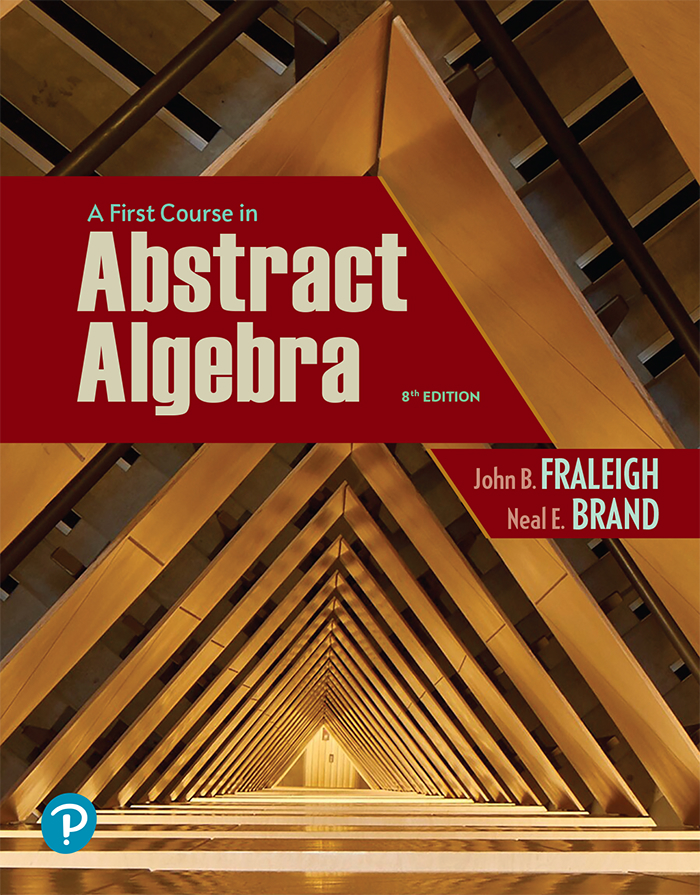
\includegraphics[width=0.960\linewidth,height=.8\textheight,keepaspectratio]{assets/front_001.pdf}\end{center}

% Source PDF page 2; original printed page 
\BookSource{2}{}
\begin{center}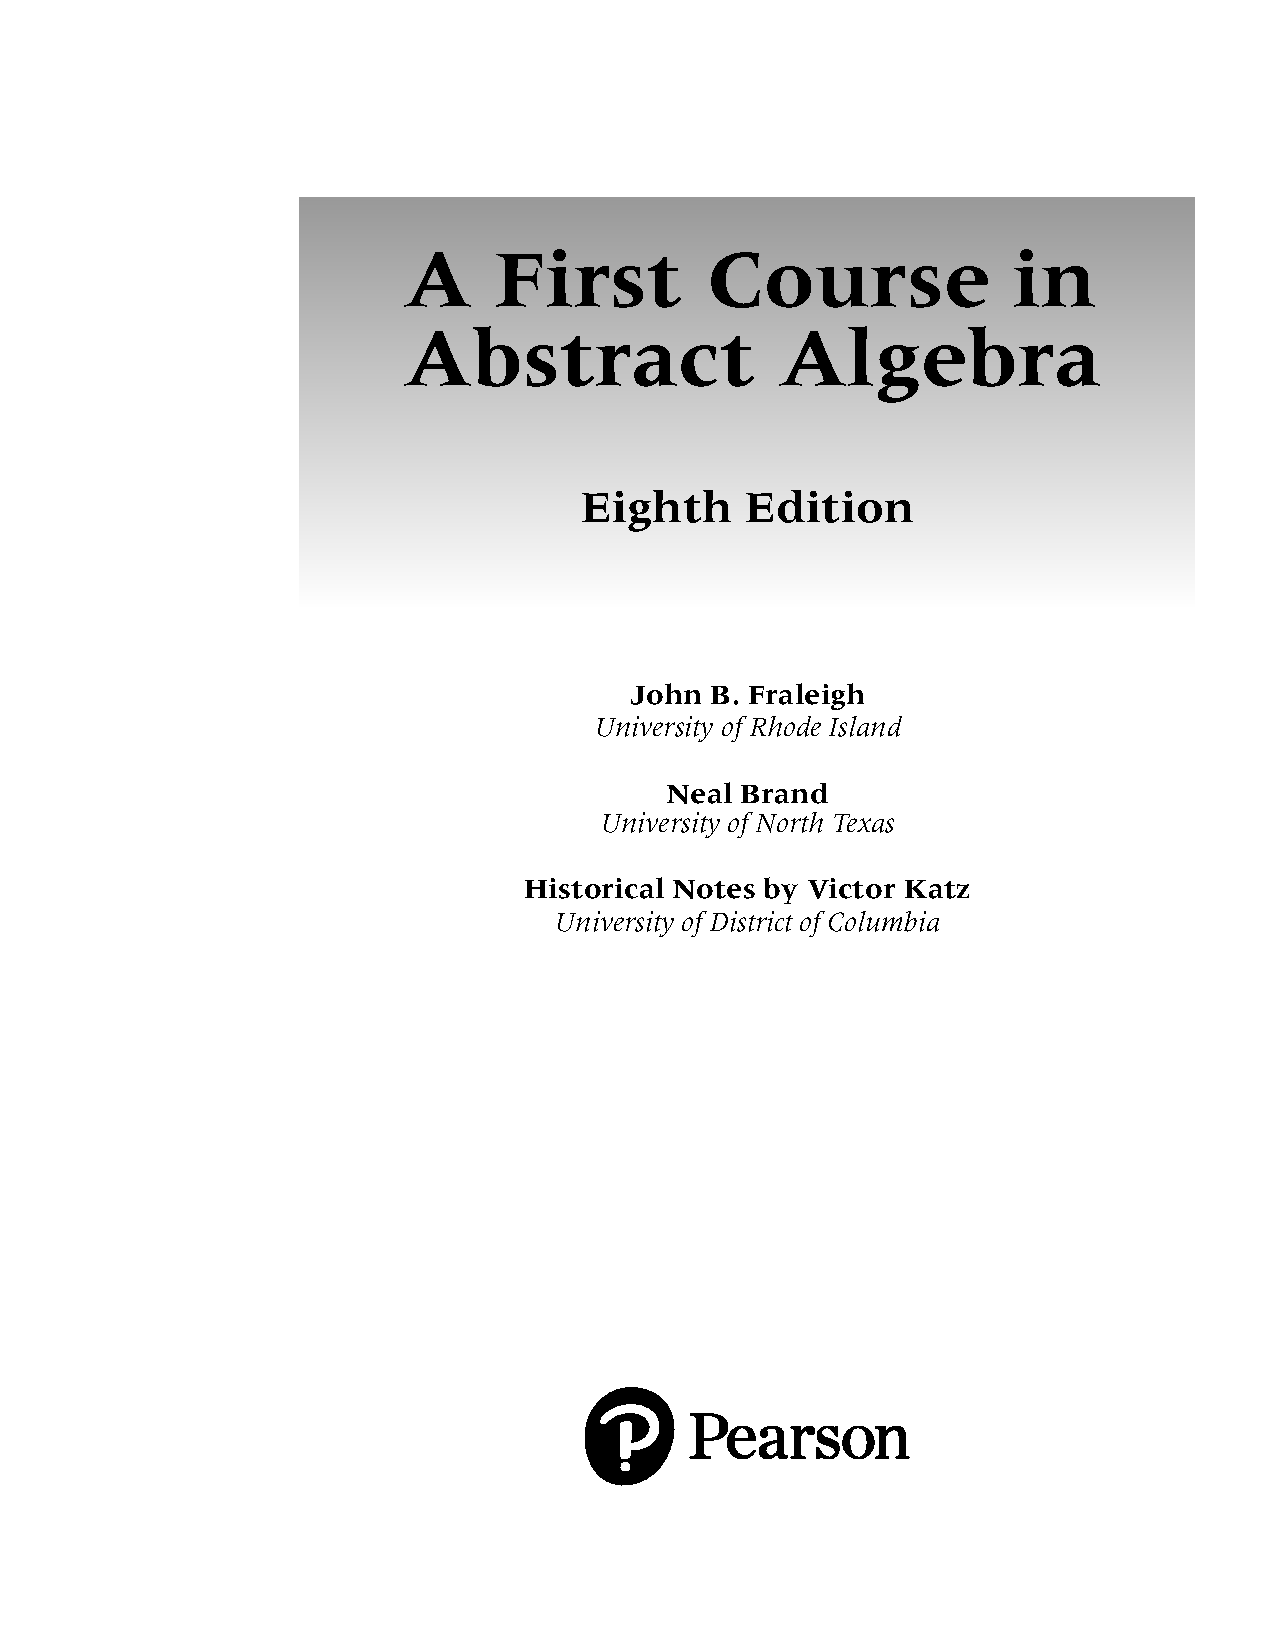
\includegraphics[width=1.000\linewidth,height=.8\textheight,keepaspectratio]{assets/front_002.pdf}\end{center}

% Source PDF page 3; original printed page 
\BookSource{3}{}
\BookNarrativefalse

\begin{BookBody}

\footnotesize

\noindent Copyright \BookInline{\text{\copyright} }c 2021, 2003, 1994 by Pearson Education, Inc. or its affiliates, 221 River Street, Hoboken, NJ 07030. All Rights Reserved. Manufactured in the United States of America. This publication is protected by copyright, and permission should be obtained from the publisher prior to any prohibited reproduction, storage in a retrieval system, or transmission in any form or by any means, electronic, mechanical, photocopying, recording, or otherwise. For information regarding permissions, request forms, and the appropriate contacts within the Pearson Education Global Rights and Permissions department, please visit \url{www.pearsoned.com/permissions/.}

\noindent Acknowledgments of third-party content appear on the appropriate page within the text.

\noindent Cover image credit: Edmund Sumner/AGE Fotostock

\noindent PEARSON, ALWAYS LEARNING, and MYLAB are exclusive trademarks owned by Pearson Education, Inc. or its affiliates in the U.S. and/or other countries.

\noindent Unless otherwise indicated herein, any third-party trademarks, logos, or icons that may appear in this work are the property of their respective owners, and any references to third-party trademarks, logos, icons, or other trade dress are for demonstrative or descriptive purposes only. Such references are not intended to imply any sponsorship, endorsement, authorization, or promotion of Pearson’s products by the owners of such marks, or any relationship between the owner and Pearson Education, Inc., or its affiliates, authors, licensees, or distributors.

\BookTextHeading{\textbf{Library of Congress Cataloging-in-Publication Data}  }

\noindent Names: Fraleigh, John B., author\BookInline{.|} Katz, Victor J., writer of added commentary.

\noindent Title: A first course in abstract algebra / John B. Fraleigh; historical notes by Victor Katz.

\noindent Description: Eighth edition\BookInline{.|[}Hoboken, New Jersey]: Pearson\BookInline{,\allowbreak [2021]|}

\noindent Series: World student series \BookInline{|} Includes bibliographical references and index.

\noindent Identifiers: LCCN \BookInline{2019038536|} ISBN 9780135758168 (paperback\BookInline{)\; |} ISBN 9780321390363 (ebook)

\noindent Subjects: LCSH: Algebra, Abstract.

\noindent Classification: LCC QA162.F\BookInline{72020|} DDC 512/.02–dc23

\noindent LC record available at \url{https://lccn.loc.gov/2019038536}

\noindent ScoutAutomatedPrintCode

Rental ISBN-10: 0-13-673162-7 ISBN-13: 978-0-13-673162-7

Loose Leaf Version

ISBN-10:

0-13-575816-5

ISBN-13: 978-0-13-575816-8

\end{BookBody}

% Source PDF page 4; original printed page 
\BookSource{4}{}
\BookHeading{Contents}
\begin{longtable}{@{}p{.83\linewidth}r@{}}
Instructor’s Preface & vii\\
Dependence Chart & xii\\
Student’s Preface & xv\\
0 Sets and Relations & 1\\
\textbf{I Groups and Subgroups} & 11\\
\hspace*{1em}1 Binary Operations & 11\\
\hspace*{1em}2 Groups & 19\\
\hspace*{1em}3 Abelian Examples & 32\\
\hspace*{1em}4 Nonabelian Examples & 39\\
\hspace*{1em}5 Subgroups & 52\\
\hspace*{1em}6 Cyclic Groups & 61\\
\hspace*{1em}7 Generating Sets and Cayley Digraphs & 70\\
\textbf{II Structure of Groups} & 77\\
\hspace*{1em}8 Groups of Permutations & 77\\
\hspace*{1em}9 Finitely Generated Abelian Groups & 88\\
\hspace*{1em}10 Cosets and the Theorem of Lagrange & 97\\
\hspace*{1em}\textsuperscript{\BookInline{\dagger}}\,11 Plane Isometries & 105\\
\textbf{III Homomorphisms and Factor Groups} & 113\\
\hspace*{1em}12 Factor Groups & 113\\
\hspace*{1em}13 Factor-Group Computations and Simple Groups & 121\\
\hspace*{1em}\textsuperscript{\BookInline{\ddagger}}\,14 Group Action on a Set & 132\\
\hspace*{1em}\textsuperscript{\BookInline{\dagger}}\,15 Applications of G-Sets to Counting & 140\\
\textbf{IV Advanced Group Theory} & 145\\
\hspace*{1em}16 Isomorphism Theorems & 145\\
\hspace*{1em}17 Sylow Theorems & 149\\
\hspace*{1em}18 Series of Groups & 157\\
\hspace*{1em}19 Free Abelian Groups & 166\\
\hspace*{1em}20 Free Groups & 172\\
\hspace*{1em}21 Group Presentations & 177\\
\textbf{V Rings and Fields} & 185\\
\hspace*{1em}22 Rings and Fields & 185\\
\hspace*{1em}23 Integral Domains & 194\\
\hspace*{1em}24 Fermat’s and Euler’s Theorems & 200\\
\hspace*{1em}25 Encryption & 205\\
\textbf{VI Constructing Rings and Fields} & 211\\
\hspace*{1em}26 the Field of Quotients of an Integral Domain & 211\\
\hspace*{1em}27 Rings of Polynomials & 218\\
\hspace*{1em}28 Factorization of Polynomials over a Field & 228\\
\hspace*{1em}\textsuperscript{\BookInline{\dagger}}\,29 Algebraic Coding Theory & 237\\
\hspace*{1em}30 Homomorphisms and Factor Rings & 243\\
\hspace*{1em}31 Prime and Maximal Ideals & 250\\
\hspace*{1em}\textsuperscript{\BookInline{\dagger}}\,32 Noncommutative Examples & 258\\
\textbf{VII Commutative Algebra} & 267\\
\hspace*{1em}33 Vector Spaces & 267\\
\hspace*{1em}34 Unique Factorization Domains & 275\\
\hspace*{1em}35 Euclidean Domains & 286\\
\hspace*{1em}36 Number Theory & 292\\
\hspace*{1em}\textsuperscript{\BookInline{\dagger}}\,37 Algebraic Geometry & 297\\
\hspace*{1em}\textsuperscript{\BookInline{\dagger}}\,38 Gröbner Bases for Ideals & 303\\
\textbf{VIII Extension Fields} & 311\\
\hspace*{1em}39 Introduction to Extension Fields & 311\\
\hspace*{1em}40 Algebraic Extensions & 319\\
\hspace*{1em}\textsuperscript{\BookInline{\dagger}}\,41 Geometric Constructions & 328\\
\hspace*{1em}42 Finite Fields & 335\\
\textbf{IX Galois Theory} & 341\\
\hspace*{1em}43 Introduction to Galois Theory & 341\\
\hspace*{1em}44 Splitting Fields & 349\\
\hspace*{1em}45 Separable Extensions & 357\\
\hspace*{1em}46 Galois Theory & 364\\
\hspace*{1em}47 Illustrations of Galois Theory & 372\\
\hspace*{1em}48 Cyclotomic Extensions & 378\\
\hspace*{1em}49 Insolvability of the Quintic & 384\\
Appendix: Matrix Algebra & 391\\
Bibliography & 395\\
Notations & 397\\
Answers to Odd-numbered Exercises Not Asking for Definitions or Proofs & 401\\
Index & 419\\
\end{longtable}
{\footnotesize\noindent \BookInline{\dagger} Not required for the remainder of the text.\par\noindent \BookInline{\ddagger} This section is a prerequisite for Sections 17 and 36 only.\par}

% Source PDF page 5; original printed page iv
\BookSource{5}{iv}


% Source PDF page 6; original printed page v
\BookSource{6}{v}


% Source PDF page 8; original printed page 
\BookSource{8}{}
\BookNarrativetrue

\begin{BookBody}

\BookTextHeading{\textbf{Instructor’s Preface}  }

\noindent This is an introduction to abstract algebra. It is anticipated that the students have studied calculus and probably linear algebra. However, these are primarily\textit{ mathematical ma}\textit{turity} prerequisites; subject matter from calculus and linear algebra appears mostly in illustrative examples and exercises.

As in previous editions of the text, our aim remains to teach students as much about groups, rings, and fields as we can in a first course. For many students, abstract algebra is their first extended exposure to an axiomatic treatment of mathematics. Recognizing this, we have included extensive explanations concerning what we are trying to accomplish, how we are trying to do it, and why we choose these methods. Mastery of this text constitutes a firm foundation for more specialized work in algebra and also provides valuable experience for any further axiomatic study of mathematics.

\BookTextHeading{\textbf{New to This Edition}  }

\noindent [Editor’s Note: You may have noticed something new on the cover of the book. Another author! I am thrilled that Neal Brand agreed to update this classic text. He has done so carefully and thoughtfully, staying true to the spirit in which it was written. Neal’s years of experience teaching the course with this text at the University of North Texas have helped him produce a meaningful and worthwhile update to John Fraleigh’s work.]

\BookTextHeading{\textit{\textbf{Updates for the eText}}  }

\noindent A focus of this revision was transforming it from a primarily print-based learning tool to a digital learning tool. The eText is therefore filled with content and tools that will help bring the content of the course to life for students in new ways and help you improve instruction. Specifically,

\BookBullet{\textbf{Mini lectures.} These brief author-created videos for each section of the text give an overview to the section but not every example or proof. Some sections will have two videos. I have used these videos effectively with my students, who were assigned to watch them ahead of the lecture on that topic. Students came to class with a basic overview of the topic of the day, which had the effect of reducing lecture time and increasing the class time used for discussion and student 
% Source PDF page 9; original printed page viii
\BookSource{9}{viii}
presentations. Students reported that the videos were helpful in giving an overview of the topics and a better understanding of the concepts and proofs. Students were also encouraged to view the videos after the topic was covered in class to reinforce what they learned. Many students also used the videos to review topics while preparing for exams. Although I have not attempted to flip the classroom, my intention was to provide sufficient resources in the eText to make it feasible without requiring other resources.}

\end{BookBody}

\BookNarrativetrue

\begin{BookBody}

\BookBullet{\textbf{Key idea quizzes.} A database of definitions and named theorems will allow students to quiz themselves on these key ideas. The database can be used in the way that flash cards were traditionally used.}

\BookBullet{\textbf{Self-assessments.} Occasional questions interspersed in the narrative allow students to check their understanding of new ideas.}

\BookBullet{\textbf{Interactive figures and utilities.} I have added a number of opportunities for students to interact with content in a dynamic manner in order to build or enhance understanding. Interactive figures allow students to explore concepts geometrically or computationally in ways that are not possible without technology.}

\BookBullet{\textbf{Notes, Labels, and Highlights.} Notes allow instructors to add their personal teaching style to important topics, call out need-to-know information, or clarify difficult concepts. Students can make their eText their own by creating highlights with meaningful labels and notes, helping them focus on what they need to study. The customizable Notebook allows students to filter, arrange, and group their notes in a way that makes sense to them.}

\BookBullet{\textbf{Dashboard.} Instructors can create reading assignments and see the time spent in the eText so that they can plan more effective instruction.}

\BookBullet{\textbf{Portability.} Portable access lets students read their eText whenever they have a moment in their day, on Android and iOS mobile phones and tablets. Even without an Internet connection, offline reading ensures students never miss a chance to learn.}

\BookBullet{\textbf{Ease-of-Use.} Straightforward setup makes it easy for instructors to get their class up and reading quickly on the first day of class. In addition, Learning Management System (LMS) integration provides institutions, instructors, and students with single sign-on access to the eText via many popular LMSs.}

\BookTextHeading{\textit{\textbf{Exercises}}}

\noindent Many exercises in the text have been updated, and many are new. In order to prevent students from using solutions from the previous edition, I purposefully replaced or reworded some exercises.

I created an Instructor Solutions Manual, which is available online at \url{www.pearson.com} to instructors only. Solutions to exercises involving proofs are often sketches or hints, which would not be in the proper form to turn in.

\BookTextHeading{\textit{\textbf{Text Organization Modifications}}  }

\noindent For each part of the text, I provide an overview of the changes followed by significant changes to sections. In cases where changes to parts or sections were minor, I have not included a list of changes.

\noindent Part I: Groups and Subgroups

\BookBullet{Overview of changes: My main goals were to define groups and to introduce the symmetric and dihedral groups as early as possible. The early introduction of these 
% Source PDF page 10; original printed page ix
\BookSource{10}{ix}
groups provides students with examples of finite groups that are consistently used throughout the book.}

\end{BookBody}

\BookNarrativetrue

\begin{BookBody}

\BookBullet{Section 1 (Binary Operations). Former Section 2. Added definition of an identity for a binary operation.}

\BookBullet{Section 2 (Groups). Former Section 4. Included the formal definition of a group isomorphism.}

\BookBullet{Section 3 (Abelian Examples). Former Section 1. Included definition of circle group\BookInline{,\allowbreak R_{a},\allowbreak } and \BookInline{Z_{n}.} Used circle group to show associativity of \BookInline{Z_{n}} and \BookInline{R_{a}.}}

\BookBullet{Section 4 (Nonabelian Examples). Based on parts of former Sections 5, 8, and 9. Defined dihedral group and symmetric group. Gave a standardized notation for the dihedral group that is used consistently throughout the book. Introduced both two-row and cycle notation for the symmetric group}

\BookBullet{Section 5 (Subgroups). Former Section 5. Included statement of two other conditions that imply a subset is a subgroup and kept the proofs in the exercise section. Made minor modifications using examples from new Section 4.}

\BookBullet{Section 6 (Cyclic Groups). Former Section 6. Added examples using dihedral group and symmetric group.}

\BookBullet{Section 7 (Generating Sets and Cayley Digraphs). Minor modification of former Section 7.}

\BookTextHeading{Part II: Structure of Groups  }

\BookBullet{Overview of changes: The main goal was to give the formal definition of homomorphism earlier in order to simplify the proofs of Cayley’s and Lagrange’s theorems.}

\BookBullet{Section 8 (Groups of Permutations). Included formal definition of homomorphism. Based on parts of former Sections 8, 9, and 13. Used two-row permutation notation to motivate Cayley’s theorem before proof. Deleted first part of section 13 (covered in Section 4). Omitted determinant proof of even/odd permutations since definition of determinant usually uses sign of a permutation. Kept orbit counting proof. Put determinant proof and inversion counting proof in exercises.}

\BookBullet{Section 9 (Finitely Generated Abelian Groups). Former Section 11. Added the invariant factor version of the theorem. Showed how to go back and forth between the two versions of the fundamental theorem.}

\BookBullet{Section 10 (Cosets and the Theorem of Lagrange). Former Section 10. Changed the order by putting Lagrange’s Theorem first, motivating \BookInline{G/H} later in the section.}

\BookBullet{Section 11 (Plane Isometries). Minor modification of former Section 12.}

\BookTextHeading{Part III: Homomorphisms and Factor Groups  }

\BookBullet{Overview of changes: My main goal was to include a few more examples to motivate the theory and give an introduction to using group actions to prove properties of groups.}

\BookBullet{Sections 12-15 are based on former Sections 14-17, respectively.}

\BookBullet{Section 12 (Factor Groups). Started section with \BookInline{Z/nZ} example to motivate general construction. Defined factor groups from normal subgroups first instead of from homomorphisms. After developing factor groups, showed how they are formed from homomorphisms.}

\BookBullet{Section 13 (Factor-Group Computations and Simple Groups). Added a few more examples of computing factor groups. Explicitly used the fundamental homomorphism theorem in computation examples.}

\end{BookBody}

% Source PDF page 11; original printed page x
\BookSource{11}{x}
\BookNarrativetrue

\begin{BookBody}

\BookBullet{Section 14 (Group Action on a Set). Expanded examples of the general linear group and the dihedral group acting on sets. Added some applications of group actions to finite groups in anticipation of the Sylow Theorems, including Cauchy’s Theorem and that fact that \BookInline{p-}groups have a nontrivial center.}

\BookBullet{Section 15 (Applications of \BookInline{G-}sets to Counting). Minor modifications.}

\BookTextHeading{Part IV: Advanced Group Theory  }

\BookBullet{Overview of changes: I moved this part to be closer to the rest of the group theory sections. More examples were included to help clarify the concepts.}

\BookBullet{Section 16 (Isomorphism Theorems). Former Section 3. Added two examples and rewrote proofs of two theorems.}

\BookBullet{Section 17 (Sylow Theorems). Former Sections 36 and 37. Since Cauchy’s Theorem and a few other theorems leading to the Sylow Theorems were covered in new Section 14, this material was removed and the old Sections 36 and 37 were combined. A few examples and exercises were added and a proof was rewritten.}

\BookBullet{Section 18 (Series of Groups). Former Section 35. The proof of the Zassenhaus Lemma was placed after the theorem instead of making the argument before stating the theorem. One example added.}

\BookBullet{Sections 19 (Free Abelian Groups), 20 (Free Groups), and 21 (Group Presentations). Minor modifications of former Sections 38–40.}

\BookTextHeading{Part V: Rings and Fields  }

\BookBullet{Overview of changes: The previous Part IV was split into two parts, one giving an introduction and the second giving methods of constructing rings and fields.}

\BookBullet{Section 22 (Rings and Fields). Minor modification of former Section 18.}

\BookBullet{Section 23 (Integral Domains). Former Section 19. Changed former Theorem 19.3 to classify all elements in \BookInline{Z_{n}.} Added corollary that \BookInline{Z_{p}} is a field, anticipating the theorem that all finite integral domains are fields.}

\BookBullet{Section 24 (Fermat’s and Euler’s Theorems). Former Section 20. Simplified proof of Euler’s generalization using classification of elements in \BookInline{Z_{n}.}}

\BookBullet{Section 25 (Encryption). New section outlining how RSA encryption works. This provides a nice application of the material in Section 24.}

\BookTextHeading{Part VI: Constructing Rings and Fields  }

\BookBullet{Overview of changes: Part VI includes sections from the previous Parts IV and V. The change emphasizes construction techniques used to form rings and fields.}

\BookBullet{Section 26 (The Field of Quotients of an Integral Domain). Former Section 21. Rewrote the introduction to include two examples of integral domains and their field of quotients to motivate the general construction.}

\BookBullet{Section 27 (Rings of Polynomials). Minor modification of former Section 22.}

\BookBullet{Section 28 (Factorization of Polynomials over a Field). Former Section 23. Rewrote former Theorem 23.1 by making a lemma showing how to reduce degree of polynomials in set \BookInline{S.} Included proof of former 23.11 in the exercises.}

\BookBullet{Section 29 (Algebraic Coding Theory). New section introducing coding theory, focusing on polynomial codes. This gives an application of polynomial computation over a finite field.}

\BookBullet{Section 30 (Homomorphisms and Factor Rings). Former Section 26. Motivated why you need the usual conditions for an ideal by starting the section with the example of \BookInline{Z/nZ.} Rearranged the order by showing that \BookInline{I} an ideal of \BookInline{R} gives rise 
% Source PDF page 12; original printed page xi
\BookSource{12}{xi}
to the factor ring \BookInline{R/I,\allowbreak } then included the material on homomorphisms and factor rings from the kernel. Expanded the statement of former Theorem 26.3 to make it easier to read and more approachable.}

\end{BookBody}

\BookNarrativetrue

\begin{BookBody}

\BookBullet{Section 31 (Prime and Maximal Ideals). Minor modification of former Section 27.}

\BookBullet{Section 32 (Noncommutative Examples). Minor modification of former Section 24.}

\BookTextHeading{Part VII: Commutative Algebra  }

\BookBullet{Overview of changes: This part includes sections that fit under the general heading of commutative algebra.}

\BookBullet{Section 33 (Vector Spaces). Former Section 30. Added two examples and a brief introduction to \BookInline{R-}modules over a ring motivated by vector spaces and abelian groups. Moved Former Theorem 30.23 to Section 45 on field extensions.}

\BookBullet{Section 34 (Unique Factorization Domains). Former Section 45. Included definition of a Noetherian ring and made other minor changes.}

\BookBullet{Section 35 (Euclidean Domains) and Section 36 (Number Theory) are minor modifications of Sections 46 and 47, respectively.}

\BookBullet{Section 37 (Algebraic Geometry). Based on the first half of former Section 28. Added a proof of the Hilbert Basis Theorem.}

\BookBullet{Section 38 (Gröbner Bases for Ideals). Based on the second half of former Section 28. Added two applications of Gröbner Bases: deriving the formulas for conic sections and determining if a graph can be colored with \BookInline{k} colors.}

\BookTextHeading{Part VIII: Extension Fields  }

\BookBullet{Overview of changes: Part VIII consists of minor changes from former Part VI.}

\BookBullet{Section 39 (Introduction to Extension Fields). Former Section 29. Divided former Theorem 29.13 into a theorem and a corollary. Rewrote former Theorem 29.18 and its proof to make it easier to follow. Included example moved from former Section 30.}

\BookBullet{Section 40 (Algebraic Extensions), Section 41 (Geometric Constructions), and Section 42 (Finite Fields) are minor modifications of former Sections 31–33, respectively.}

\BookTextHeading{Part IX: Galois Theory  }

\BookBullet{Overview of changes: The previous Part X was rewritten to form Part IX. The goal was to improve the readability of the material while maintaining a rigorous development of the theory.}

\BookBullet{Section 43 (Introduction to Galois Theory). New section. Uses the field extension \BookInline{Q(\sqrt{2},\allowbreak \sqrt{3})} throughout to motivate and illustrate basic definitions and theorems including field automorphism, field fixed by an automorphism, group of automorphisms fixing a subfield, conjugates, and the conjugate isomorphism theorem. By using an easy-to-understand example consistently throughout, the concepts become more concrete.}

\BookBullet{Section 44 (Splitting Fields). Includes the contents of former Sections 49 and 50, but it is completely rewritten. Less emphasis is given to the algebraic closure of a field and more emphasis is given to subfields of splitting fields.}

\BookBullet{Section 45 (Separable Extensions). Contents include most of former Section 51 and a little from former Section 53, but material has been rewritten. The notation \BookInline{\{}E:F\BookInline{\}} was omitted and definition of separable was given in terms of multiplicity of zeros. Emphasized subfields of the complex numbers.}

\end{BookBody}

% Source PDF page 13; original printed page xii
\BookSource{13}{xii}
\BookNarrativetrue

\begin{BookBody}

\BookBullet{Former Section 52 on totally inseparable extensions was omitted since it was not used elsewhere and it detracts from the flow of the rest of Part IX.}

\BookBullet{Section 46 (Galois Theory). Former Section 53. Separated the parts of Galois Theory into separate theorems. Continued the same example throughout the section to motivate and illustrate the theorems. By the end of the section, the continued example illustrates how Galois Theory can be used.}

\BookBullet{Section 47 (Illustrations of Galois Theory). Minor modification of former Section 54.}

\BookBullet{Section 48 (Cyclotomic Extensions). Former Section 55. In order to make the text more readable, restricted the field extensions to subfields of the complex numbers over the rational numbers since this is the only case that is used in the book.}

\BookBullet{Section 49 (Insolvability of the Quintic). Former Section 56. Replaced construction of a polynomial that is not solvable by radicals with a specific concrete polynomial. The previous construction of a nonsolvable polynomial was moved to the exercises.}

\noindent Part X: Groups in Topology (Online at bit.ly/2VBCiej)

\BookBullet{Sections 50-53 are minor modifications of former sections 41-44.}

\BookTextHeading{\textbf{Some Features Retained}  }

\noindent I continue to break down most exercise sets into parts consisting of computations, concepts, and theory. Answers to most odd-numbered exercises not requesting a proof again appear at the back of the text. I am supplying the answers to parts a, c, e, g, and i only of our 10-part true-false exercises. The excellent historical notes by Victor Katz are, of course, retained.

\BookTextHeading{\textbf{Suggestions for New Instructors of Algebra}  }

\noindent Those who have taught algebra several times have discovered the difficulties and developed their own solutions. The comments we make here are not for them.

This course is an abrupt change from the typical undergraduate calculus for the students. A graduate-style lecture presentation, writing out definitions and proofs on the board for most of the class time, will not work with most students. We have found it best to spend at least the first half of each class period answering questions on homework, trying to get a volunteer to give a proof requested in an exercise, and generally checking to see if they seem to understand the material assigned for that class. Typically, we spent only about the last 20 minutes of our 50-minute time talking about new ideas for the next class, and giving at least one proof. The videos for each section can effectively be used to supplement or replace lectures. From a practical point of view, it is a waste of time to try to write on the board all the definitions and proofs. They are in the text.

We suggest that at least half of the assigned exercises consist of the computational ones. Students are used to doing computations in calculus. Although there are many exercises asking for proofs that we would love to assign, we recommend that you assign at most two or three such exercises and try to get someone to explain how each proof is performed in the next class. We do think students should be asked to do at least one proof in each assignment.

Students face a barrage of definitions and theorems, something they have never encountered before. They are not used to mastering this type of material. Grades on tests that seem reasonable to us, requesting a few definitions and proofs, are apt to be low and depressing for most students and instructors. To encourage students to keep up

\end{BookBody}

% Source PDF page 14; original printed page xiii
\BookSource{14}{xiii}
\BookNarrativetrue

\begin{BookBody}

\begin{BookFloat}{front_matter-p14-0}
\begin{center}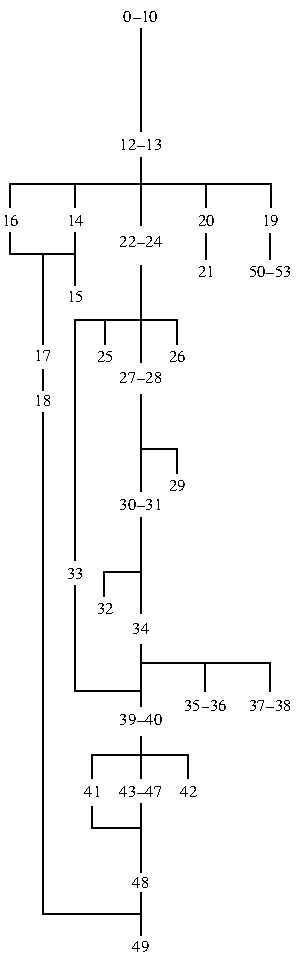
\includegraphics[width=0.409\linewidth,height=.8\textheight,keepaspectratio]{assets/front_dependence_chart.pdf}\end{center}
\begin{center}\textbf{Dependence Chart}\end{center}
\end{BookFloat}

\noindent with the basic material, I give approximately ten pop quizzes per semester that typically involve stating a definition, giving an example, or stating a major theorem.

At the University of North Texas, abstract algebra is a two-semester sequence. The first semester is required of all math majors and the second semester is optional. Because most students opt not to continue with the second semester, it is not offered every year. When I teach either class, I give three 50-minute in-class exams. With exam reviews and going over completed exams, this leaves approximately 36 class periods for new material.

In the first-semester class, the base material I always cover includes Sections 0-6, 8, 9, 12, 13, and 22-25. I average approximately two class periods per section, so I can usually cover a few more sections. Options I have used for the remaining time include

\end{BookBody}

% Source PDF page 15; original printed page xiv
\BookSource{15}{xiv}
\BookNarrativetrue

\begin{BookBody}

\noindent Sections 14 and 15, Sections 26-28, Section 17, or Sections 30 and 31. One semester I attempted to cover enough field extension material in order to cover Section 41. This required me to carefully select material in Sections 27, 28, 39, and 40 in order to prepare the students for Section 41.

For the second semester, I usually have as goals proving the impossibility of bisecting an angle using compass and straightedge and the insolvability of quintic polynomials. Assuming that students have seen the basic material in the first semester as described above, these goals require covering material from Sections 16, 18, 27, 28, 30, 31, 33, 34, and 39-49. This turns out to be an ambitious undertaking, but the purpose of rewriting Part IX was to make the material more accessible to students, and therefore make the goal of covering Galois Theory in a second-semester class more feasible.

\BookTextHeading{\textbf{Acknowledgments}}

\noindent I am very grateful to those who have reviewed the text or who have sent suggestions and corrections. Below is a list of faculty who contributed their thoughts on improving the text.

\BookBullet{Deb Bergstrand, Swarthmore College}

\BookBullet{Anthony E. Clement, Brooklyn College}

\BookBullet{Richard M. Green, University of Colorado}

\BookBullet{Cheryl Grood, Swarthmore College}

\BookBullet{Gary Gordon, Lafayette College}

\BookBullet{John Harding, New Mexico State University}

\BookBullet{Timothy Kohl, Boston University}

\BookBullet{Cristian Lenart, University at Albany, SUNY}

\BookBullet{Mariana Montiel, Georgia Southern University}

\BookBullet{Anne Shiu, Texas A\&M University}

\BookBullet{Mark Stankus, California Polytechnic State University}

\BookBullet{Janet Vassilev, University of New Mexico}

\BookBullet{Cassie L. Williams, James Madison University}

\BookBullet{T. E. Williamson, Montclair State University}

\BookBullet{Michael Zuker, Massachusetts Institute of Technology}

I also wish to express appreciation to Jeff Weidenaar, Tara Corpuz, and Jon Krebs at Pearson for their help with this project.

\noindent Neal Brand

\noindent University of North Texas

\end{BookBody}

% Source PDF page 16; original printed page 
\BookSource{16}{}
\BookNarrativetrue

\begin{BookBody}

\BookTextHeading{\textbf{Student’s Preface}  }

\noindent This course may well require a different approach than those you used in previous mathematics courses. You may have become accustomed to working a homework problem by turning back in the text to find a similar problem, and then just changing some numbers. That may work with a few problems in this text, but it will not work for most of them. This is a subject in which understanding is all-important, and where problems should not be tackled without first studying the text.

Let us make some suggestions on studying the text. Notice that the text bristles with definitions, theorems, corollaries, and examples. The definitions are crucial. We must agree on terminology to make any progress. Sometimes a definition is followed by an example that illustrates the concept. Examples are probably the most important aids in studying the text.\textit{ Pay attention to the examples.}

Before reading a section, it may be helpful to watch the video associated with the section. I have two general pieces of advice for watching a video or reading the text. First, minimize your distractions. It takes a good deal of concentration for most of us to learn new technical information. Second, have paper and pen (or the electronic equivalent) at hand to take notes and to occasionally work out computations on your own.

I suggest you skip the proofs of the theorems on your first reading of a section, unless you are really “gung-ho” on proofs. You should read the statement of the theorem and try to understand just what it means. Often, a theorem is followed or preceded by an example that illustrates it, which is a great aid in really understanding what the theorem says. Pay particular attention to the summary at the end of each video to get an overview of the topics covered.

In summary, on your first viewing and reading of a section, I suggest you concentrate on what information the section gives and on gaining a real understanding of it. If you do not understand what the statement of a theorem means, it will probably be meaningless for you to read the proof.

Proofs are basic to mathematics. After you feel you understand the information given in a section, you should read and try to understand at least some of the proofs. In the videos you will find a few proofs. Watching the videos a second time after you have a better understanding of the definitions and the statements of the theorems will help to clarify these proofs. Proofs of corollaries are usually the easiest ones, for they often follow directly from the theorem. Many of the exercises under the ”Theory” heading 
% Source PDF page 17; original printed page xvi
\BookSource{17}{xvi}
ask for a proof. Try not to be discouraged at the outset. It takes a bit of practice and experience. Proofs in algebra can be more difficult than proofs in geometry and calculus, for there are usually no suggestive pictures that you can draw. Often, a proof falls out easily if you happen to look at just the right expression. Of course, it is hopeless to devise a proof if you do not really understand what it is that you are trying to prove. For example, if an exercise asks you to show that a given thing is a member of a certain set, you must\textit{ know} the defining criterion for a thing to be a member of that set, and then show that your given thing satisfies that criterion.

\end{BookBody}

\BookNarrativetrue

\begin{BookBody}

There are several aids for your study at the back of the text. Of course, you will discover the answers to odd-numbered problems that do not involve a proof. If you run into a notation such as \BookInline{Z_{n}} that you do not understand, look in the list of notations that appears after the bibliography. If you run into terminology like\textit{ inner automorphism} that you do not understand, look in the index for the first page where the term occurs.

In summary, although an understanding of the subject is important in every mathematics course, it is crucial to your performance in this course. May you find it a rewarding experience.

\end{BookBody}
\ifdefined\BookMaster\let\BookFinish\relax\else\def\BookFinish{\end{document}}\fi\BookFinish

\clearpage
\pagenumbering{arabic}
% !TeX program = xelatex
\ifdefined\BookMaster\else
\documentclass[11pt,oneside]{article}
% !TeX program = xelatex
\usepackage[b5paper,left=22mm,right=22mm,top=20mm,bottom=22mm,footskip=11mm]{geometry}
\usepackage{fontspec}
\setmainfont{TeX Gyre Termes}
\setsansfont{TeX Gyre Heros}
\usepackage{amsmath,amssymb,mathtools,amsthm}
\renewcommand{\cdots}{\mathinner{\cdotp\cdotp\cdotp}}
\usepackage{graphicx,adjustbox,array,booktabs,longtable,multirow,enumitem,changepage,needspace}
\usepackage[table]{xcolor}
\usepackage{fancyhdr}
\raggedbottom
\interfootnotelinepenalty=10000
\newcommand{\BookFootnote}[2]{\begingroup\renewcommand{\thefootnote}{\fnsymbol{footnote}}\footnote[#1]{#2}\endgroup}
\newcommand{\BookFootnoteMark}[1]{\begingroup\renewcommand{\thefootnote}{\fnsymbol{footnote}}\footnotemark[#1]\endgroup}
\newcommand{\BookFootnoteText}[2]{\begingroup\renewcommand{\thefootnote}{\fnsymbol{footnote}}\footnotetext[#1]{#2}\endgroup}
\newenvironment{BookFloat}[1]{\par\addvspace{.6\baselineskip}\noindent\def\BookFloatID{#1}\begin{minipage}{\linewidth}\phantomsection\label{bookfloat:#1:start}}{\phantomsection\label{bookfloat:\BookFloatID:end}\end{minipage}\par\addvspace{.6\baselineskip}}

\usepackage[unicode,hidelinks]{hyperref}
\pagestyle{fancy}
\fancyhf{}
\newcommand{\BookFooter}{}
\fancyfoot[L]{\parbox[b]{\dimexpr\textwidth-15mm}{\footnotesize\BookFooter}}
\fancyfoot[R]{\footnotesize\thepage}
\renewcommand{\headrulewidth}{0pt}
\renewcommand{\footrulewidth}{0pt}
\setlength{\parindent}{0pt}
\setlength{\parskip}{0.2em}
\setlength{\emergencystretch}{3em}
\setlist{nosep,leftmargin=1.7em,labelsep=.65em}
\newif\ifBookNarrative
\BookNarrativetrue
\newenvironment{BookBody}{\setlength{\parindent}{0pt}}{}
\newcommand{\BookStatement}[1]{\par\addvspace{.6\baselineskip}\noindent #1\enspace\ignorespaces}
\newcommand{\BookLabel}[1]{\par\addvspace{.6\baselineskip}\needspace{3\baselineskip}\noindent\textbf{#1}\quad\ignorespaces}
\newcommand{\BookHeading}[1]{\par\addvspace{\baselineskip}\needspace{4\baselineskip}\noindent{\large\bfseries #1}\par\medskip}
\newcommand{\BookSubheading}[1]{\par\addvspace{.7\baselineskip}\needspace{3\baselineskip}\noindent{\bfseries #1}\par\smallskip}
\newcommand{\BookTextHeading}[1]{\par\addvspace{.7\baselineskip}\needspace{3\baselineskip}\noindent #1\par\smallskip}
\newcommand{\BookSectionTitle}[2]{\par\addvspace{1.2\baselineskip}\needspace{5\baselineskip}\noindent\colorbox{gray!25}{\sffamily\bfseries\small SECTION #1}\quad{\large\bfseries #2}\par\medskip}
\newcommand{\BookExerciseTitle}[1]{\par\addvspace{\baselineskip}\needspace{4\baselineskip}\noindent{\color{gray}\rule{1.5mm}{1.5mm}}\enspace{\large\bfseries Exercises #1}\par\medskip}
\newcommand{\BookBullet}[1]{\begin{list}{\textbullet}{\setlength{\leftmargin}{1.7em}\setlength{\labelwidth}{1em}\setlength{\labelsep}{.7em}\setlength{\topsep}{0pt}\setlength{\parsep}{0pt}\setlength{\itemsep}{0pt}}\item #1\end{list}}
\newcommand{\BookExercise}[2]{\begin{list}{\textbf{#1}}{\setlength{\leftmargin}{2.2em}\setlength{\labelwidth}{1.5em}\setlength{\labelsep}{.7em}\setlength{\topsep}{.15em}\setlength{\parsep}{0pt}\setlength{\itemsep}{0pt}}\item #2\end{list}}
\newcommand{\BookEnd}[1]{\unskip\nobreak\hfill\ensuremath{#1}}
\newcommand{\BookSource}[2]{\phantomsection\label{sourcepage:#1}} % Source-page anchors, retained through reflow.
\usepackage{multicol}
\usepackage{tikz}
\newcommand{\BookPartEntry}[2]{\par\noindent\makebox[17mm][l]{\bfseries Section #1}#2\par}
\newcommand{\BookPartTitle}[3]{\par\bigskip\noindent\begin{tikzpicture}\node[anchor=north west,inner sep=0pt,outer sep=0pt] (bookpart) at (0,0) {\begin{minipage}{\dimexpr\linewidth-.5pt}\hspace*{26mm}\begin{minipage}[t]{\dimexpr\linewidth-26mm}\begin{adjustbox}{max width=\linewidth}{\fontsize{20}{24}\selectfont\bfseries #2}\end{adjustbox}\par\vspace{6mm}\hrule\vspace{6mm}{\sffamily\footnotesize\setlength{\parskip}{.3em}#3}\vspace{3mm}\end{minipage}\end{minipage}};\path[shade,top color=gray!60,bottom color=white] (0,0) rectangle ([xshift=24mm]bookpart.south west);\node[anchor=north,font=\sffamily\bfseries\small] at (12mm,-2mm) {PART};\node[anchor=north,font=\sffamily\bfseries\Huge] at (12mm,-7mm) {#1};\end{tikzpicture}\par\bigskip}
\newsavebox{\BookMathBox}
\makeatletter
\newcommand{\BookInline}[1]{\leavevmode\hskip0pt\relax\begingroup\in@{\begin}{#1}\ifin@\sbox{\BookMathBox}{\(#1\)}\ifdim\wd\BookMathBox>\dimexpr\linewidth-1em\relax\resizebox{\dimexpr\linewidth-1em\relax}{!}{\usebox{\BookMathBox}}\else\(#1\)\fi\else\in@{\left}{#1}\ifin@\sbox{\BookMathBox}{\(#1\)}\ifdim\wd\BookMathBox>\dimexpr\linewidth-1em\relax\resizebox{\dimexpr\linewidth-1em\relax}{!}{\usebox{\BookMathBox}}\else\(#1\)\fi\else\(#1\)\fi\fi\endgroup\hskip0pt\relax}
\makeatother
\DeclareMathOperator{\Aut}{Aut}
\DeclareMathOperator{\End}{End}
\DeclareMathOperator{\Hom}{Hom}
\DeclareMathOperator{\GF}{GF}
\DeclareMathOperator{\irr}{irr}
\DeclareMathOperator{\lt}{lt}
\DeclareMathOperator{\lp}{lp}
\providecommand{\textcircled}[1]{\textnormal{(#1)}}

\begin{document}
\fi
\renewcommand{\BookFooter}{Section 0 Sets and Relations}
\pdfbookmark[0]{Section 0 Sets and Relations}{00_sets_and_relations}
\ifdefined\BookMaster\else\setcounter{page}{1}\fi
% Source PDF page 18; original printed page 1
\BookSource{18}{1}
\BookNarrativetrue

\begin{BookBody}

\BookSectionTitle{0}{Sets and Relations}

\BookTextHeading{\textbf{On Definitions, and the Notion of a Set}  }

\noindent Many students do not realize the great importance of definitions to mathematics. This importance stems from the need for mathematicians to communicate with each other. If two people are trying to communicate about some subject, they must have the same understanding of its technical terms. However, there is an important structural weakness.

\noindent It is impossible to define every concept.

\noindent Suppose, for example, we define the term\textit{ set} as “A\textbf{ set} is a well-defined collection of objects.” One naturally asks what is meant by a\textit{ collection.} We could define it as “A collection is an aggregate of things.” What, then, is an\textit{ aggregate?} Now our language is finite, so after some time we will run out of new words to use and have to repeat some words already examined. The definition is then circular and obviously worthless. Mathematicians realize that there must be some undefined or primitive concept with which to start. At the moment, they have agreed that\textit{ set} shall be such a primitive concept. We shall not define\textit{ set,} but shall just hope that when such expressions as “the set of all real numbers” or “the set of all members of the United States Senate” are used, people’s various ideas of what is meant are sufficiently similar to make communication feasible. We summarize briefly some of the things we shall simply assume about sets.

\BookExercise{1.}{A set \BookInline{S} is made up of\textbf{ elements,} and if \BookInline{a} is one of these elements, we shall denote this fact by \BookInline{a\in S.}}

\BookExercise{2.}{There is exactly one set with no elements. It is the\textbf{ empty set} and is denoted by \BookInline{\emptyset.}}

\BookExercise{3.}{We may describe a set either by giving a characterizing property of the elements, such as “the set of all members of the United States Senate,” or by listing the elements. The standard way to describe a set by listing elements is to enclose the designations of the elements, separated by commas, in braces, for example\BookInline{,\allowbreak \{1,\allowbreak 2,\allowbreak 15\}.} If a set is described by a characterizing property \BookInline{P(x)} of its elements \BookInline{x,\allowbreak } the brace notation \BookInline{\{x\mid P(x)\}} is also often used, and is read “the set of all \BookInline{x} such that the statement \BookInline{P(x)} about \BookInline{x} is true.” Thus}

\begin{center}\begin{adjustbox}{max width=\linewidth}\BookInline{\displaystyle \begin{aligned}\{2,\allowbreak 4,\allowbreak 6,\allowbreak 8\}&= \{x\mid x\;\text{is an even whole positive number}\;\leq 8\} \\ &= \{2x\mid x= 1,\allowbreak 2,\allowbreak 3,\allowbreak 4\}.\end{aligned}}\end{adjustbox}\end{center}

The notation \BookInline{\{x\mid P(x)\}} is often called “set-builder notation.”

\BookExercise{4.}{A set is\textbf{ well defined,} meaning that if \BookInline{S} is a set and \BookInline{a} is some object, then either \BookInline{a} is definitely in \BookInline{S,\allowbreak } denoted by \BookInline{a\in S,\allowbreak } or \BookInline{a} is definitely not in \BookInline{S,\allowbreak } denoted by \BookInline{a\notin S.} Thus, we should never say, “Consider the set \BookInline{S} of some positive numbers,” for it is not definite whether \BookInline{2\in S} or \BookInline{2\notin S.} On the other hand, we can consider the set \BookInline{T} of all prime positive integers. Every positive integer is definitely either prime or not prime. Thus \BookInline{5\in T} and \BookInline{14\notin T.} It may be hard to actually determine whether an object is in a set. For example, as this book goes to press it is probably unknown whether \BookInline{2^{(2^{65})}+ 1} is in \BookInline{T.} However, \BookInline{2^{(2^{65})}+ 1} is certainly either prime or not prime.}

\end{BookBody}

% Source PDF page 19; original printed page 2
\BookSource{19}{2}
\BookNarrativetrue

\begin{BookBody}

It is not feasible for this text to push the definition of everything we use all the way back to the concept of a set. For example, we will never define the number \BookInline{\pi } in terms of a set.

Every definition is an\textit{ if and only if} type of statement.

With this understanding, definitions are often stated with the\textit{ only if} suppressed, but it is always to be understood as part of the definition. Thus we may define an isosceles triangle as follows: “A triangle is\textbf{ isosceles} if it has two congruent sides” when we really mean that a triangle is isosceles\textit{ if and only if} it has two congruent sides.

In our text, we have to define many terms. We use specifically labeled and numbered definitions for the main algebraic concepts with which we are concerned. To avoid an overwhelming quantity of such labels and numberings, we define many terms within the body of the text and exercises using boldface type.

\BookTextHeading{\textbf{Boldface Convention}  }

A term printed\textbf{ in boldface} in a sentence is being defined by that sentence.

Do not feel that you have to memorize a definition word for word. The important thing is to\textit{ understand} the concept, so that you can define precisely the same concept in your own words. Thus the definition “An\textbf{ isosceles} triangle is one having two sides of equal length” is perfectly correct. Of course, we had to delay stating our boldface convention until we had finished using boldface in the preceding discussion of sets, because we do not define a set!

In this section, we do define some familiar concepts as sets, both for illustration and for review of the concepts. First we give a few definitions and some notation.

\BookLabel{0.1 Definition} A set \BookInline{B} is a\textbf{ subset of a set} \BookInline{A,\allowbreak } denoted by \BookInline{B\subseteq A} or \BookInline{A\supseteq B,\allowbreak } if every element of \BookInline{B} is in \BookInline{A.} The notations \BookInline{B\subset A} or \BookInline{A\supset B} will be used for \BookInline{B\subseteq A} but \BookInline{B\neq A.}\BookEnd{\blacksquare}

\noindent Note that according to this definition, for any set \BookInline{A,\allowbreak A} itself and \BookInline{\emptyset } are both subsets of \BookInline{A.}

\BookLabel{0.2 Definition} If \BookInline{A} is any set, then \BookInline{A} is the\textbf{ improper subset of} \BookInline{A.} Any other subset of \BookInline{A} is a\textbf{ proper} \textbf{subset of} \BookInline{A.}\BookEnd{\blacksquare}

\BookLabel{0.3 Example} Let \BookInline{S= \{1,\allowbreak 2,\allowbreak 3\}.} This set \BookInline{S} has a total of eight subsets, namely \BookInline{\emptyset,\allowbreak \{1\},\allowbreak \{2\},\allowbreak \{3\},\allowbreak } \BookInline{\{1,\allowbreak 2\},\allowbreak \{1,\allowbreak 3\},\allowbreak \{2,\allowbreak 3\},\allowbreak } and \BookInline{\{1,\allowbreak 2,\allowbreak 3\}.}\BookEnd{\blacktriangle}

\BookLabel{0.4 Definition} Let \BookInline{A} and \BookInline{B} be sets. The set \BookInline{A\times B= \{(a,\allowbreak b)\mid a\in A} and \BookInline{b\in B\}} is the\textbf{ Cartesian product} of \BookInline{A} and \BookInline{B.}\BookEnd{\blacksquare}

\BookLabel{0.5 Example} If \BookInline{A= \{1,\allowbreak 2,\allowbreak 3\}} and \BookInline{B= \{3,\allowbreak 4\},\allowbreak } then we have

\begin{center}\begin{adjustbox}{max width=\linewidth}\BookInline{\displaystyle A\times B= \{(1,\allowbreak 3),\allowbreak (1,\allowbreak 4),\allowbreak (2,\allowbreak 3),\allowbreak (2,\allowbreak 4),\allowbreak (3,\allowbreak 3),\allowbreak (3,\allowbreak 4)\}.}\end{adjustbox}\end{center} \BookEnd{\blacktriangle}

Throughout this text, much work will be done involving familiar sets of numbers. Let us take care of notation for these sets once and for all.

\BookInline{\mathbb{Z}} is the set of all integers (that is, whole numbers: positive, negative, and zero).

\BookInline{\mathbb{Q}} is the set of all rational numbers (that is, numbers that can be expressed as quotients \BookInline{m/n} of integers, where \BookInline{n\neq 0).}

\end{BookBody}

% Source PDF page 20; original printed page 3
\BookSource{20}{3}
\BookNarrativetrue

\begin{BookBody}

\BookInline{\mathbb{R}} is the set of all real numbers.

\BookInline{\mathbb{Z}^{+ },\allowbreak \mathbb{Q}^{+ },\allowbreak } and \BookInline{\mathbb{R}^{+ }} are the sets of positive members of \BookInline{\mathbb{Z},\allowbreak \mathbb{Q},\allowbreak } and \BookInline{\mathbb{R},\allowbreak } respectively.

\BookInline{\mathbb{C}} is the set of all complex numbers.

\BookInline{\mathbb{Z}^{\ast },\allowbreak \mathbb{Q}^{\ast },\allowbreak \mathbb{R}^{\ast },\allowbreak } and \BookInline{\mathbb{C}^{\ast }} are the sets of nonzero members of \BookInline{\mathbb{Z},\allowbreak \mathbb{Q},\allowbreak \mathbb{R},\allowbreak } and \BookInline{\mathbb{C},\allowbreak } respectively.

\BookLabel{0.6 Example} The set \BookInline{\mathbb{R}\times \mathbb{R}} is the familiar Euclidean plane that we use in first-semester calculus to draw graphs of functions\BookInline{.}\BookEnd{\blacktriangle}

\BookTextHeading{\textbf{Relations Between Sets}  }

\noindent We introduce the notion of an element \BookInline{a} of set \BookInline{A} being\textit{ related} to an element \BookInline{b} of set \BookInline{B,\allowbreak } which we might denote by \BookInline{a\mathcal{R}b.} The notation \BookInline{a\mathcal{R}b} exhibits the elements \BookInline{a} and \BookInline{b} in left-to-right order, just as the notation \BookInline{(a,\allowbreak b)} for an element in \BookInline{A\times B.} This leads us to the following definition of a relation \BookInline{\mathcal{R}} as a\textit{ set}.

\BookLabel{0.7 Definition} A\textbf{ relation} between sets \BookInline{A} and \BookInline{B} is a subset \BookInline{\mathcal{R}} of \BookInline{A\times B.} We read \BookInline{(a,\allowbreak b)\in \mathcal{R}} as “\BookInline{a} is related to \BookInline{b}” and write \BookInline{a\mathcal{R}b.}\BookEnd{\blacksquare}

\BookLabel{0.8 Example} Let \BookInline{S} be any set. We can define an\textbf{ Equality Relation} \BookInline{= } between \BookInline{S} and itself as the subset \BookInline{\{(x,\allowbreak x)\mid x\in S\}.} Of course, this is nothing new. It is simply the usual idea of what it means for two “things” to be equal. So if \BookInline{x,\allowbreak y\in S} are different elements, then they are not related by the equality relation and we write \BookInline{x\neq y,\allowbreak } but if \BookInline{x} and \BookInline{y} are the same then we write \BookInline{x= y.}\BookEnd{\blacktriangle}

We will refer to any relation between a set \BookInline{S} and itself, as in the preceding example, as a\textbf{ relation on} \BookInline{S.}

\BookLabel{0.9 Example} The graph of the function \BookInline{f} where \BookInline{f(x)= x^{3}} for all \BookInline{x\in \mathbb{R},\allowbreak } is the subset \BookInline{\{(x,\allowbreak x^{3})\mid x\in \mathbb{R}\}} of \BookInline{\mathbb{R}\times \mathbb{R}.} Thus it is a relation on \BookInline{\mathbb{R}.} The function is completely determined by its graph. \BookEnd{\blacktriangle}

The preceding example suggests that rather than define a “function” \BookInline{y= f(x)} to be a “rule” that assigns to each \BookInline{x\in \mathbb{R}} exactly one \BookInline{y\in \mathbb{R},\allowbreak } we can easily describe it as a certain type of subset of \BookInline{\mathbb{R}\times \mathbb{R},\allowbreak } that is, as a type of relation. We free ourselves from \BookInline{\mathbb{R}} and deal with any sets \BookInline{X} and \BookInline{Y.}

\BookLabel{0.10 Definition} A\textbf{ function} \BookInline{\phi } mapping \BookInline{X} into \BookInline{Y} is a relation between \BookInline{X} and \BookInline{Y} with the property that each \BookInline{x\in X} appears as the first member of exactly one ordered pair \BookInline{(x,\allowbreak y)} in \BookInline{\phi.} Such a function is also called a\textbf{ map} or\textbf{ mapping} of \BookInline{X} into \BookInline{Y.} We write \BookInline{\phi:X\to Y} and express \BookInline{(x,\allowbreak y)\in \phi } by \BookInline{\phi (x)= y.} The\textbf{ domain} of \BookInline{\phi } is the set \BookInline{X} and the set \BookInline{Y} is the\textbf{ codomain} of \BookInline{\phi.} The\textbf{ range} of \BookInline{\phi } is \BookInline{\phi [X]= \{\phi (x)\mid x\in X\}.}\BookEnd{\blacksquare}

\BookLabel{0.11 Example} We can view the addition of real numbers as a function \BookInline{+:(\mathbb{R}\times \mathbb{R})\to \mathbb{R},\allowbreak } that is, as a mapping of \BookInline{\mathbb{R}\times \mathbb{R}} into \BookInline{\mathbb{R}.} For example, the action of \BookInline{+ } on \BookInline{(2,\allowbreak 3)\in \mathbb{R}\times \mathbb{R}} is given in function notation by \BookInline{+ ((2,\allowbreak 3))= 5.} In set notation we write \BookInline{((2,\allowbreak 3),\allowbreak 5)\in +.} Of course, our familiar notation is \BookInline{2+ 3= 5.}\BookEnd{\blacktriangle}

\BookTextHeading{\textbf{Cardinality}}

\noindent The number of elements in a set \BookInline{X} is the\textbf{ cardinality} of \BookInline{X} and is often denoted by \BookInline{|X|.} For example, we have \BookInline{|\{2,\allowbreak 5,\allowbreak 7\}|= 3.} It will be important for us to know whether two sets have the same cardinality. If both sets are finite, there is no problem; we can simply count the elements in each set. But do \BookInline{\mathbb{Z},\allowbreak \mathbb{Q},\allowbreak } and \BookInline{\mathbb{R}} have the same cardinality?

\end{BookBody}

% Source PDF page 21; original printed page 4
\BookSource{21}{4}
\BookNarrativetrue

\begin{BookBody}

\noindent To convince ourselves that two sets \BookInline{X} and \BookInline{Y} have the same cardinality, we try to exhibit a pairing of each \BookInline{x} in \BookInline{X} with only one \BookInline{y} in \BookInline{Y} in such a way that each element of \BookInline{Y} is also used only once in this pairing. For the sets \BookInline{X= \{2,\allowbreak 5,\allowbreak 7\}} and \BookInline{Y= \{}?\BookInline{,\allowbreak!,\allowbreak } \#\BookInline{\},\allowbreak } the pairing

\begin{center}\begin{adjustbox}{max width=\linewidth}\BookInline{\displaystyle 2\leftrightarrow ?,\allowbreak 5\leftrightarrow \#,\allowbreak 7\leftrightarrow !}\end{adjustbox}\end{center}

\noindent shows they have the same cardinality. Notice that we could also exhibit this pairing as \BookInline{\{(2,\allowbreak }?), (5, \#), (7,!\BookInline{)\}} which, as a subset of \BookInline{X\times Y,\allowbreak } is a\textit{ relation} between \BookInline{X} and \BookInline{Y.} The pairing

\begin{BookFloat}{00_sets_and_relations-p21-3}
\begin{center}\begin{adjustbox}{max width=\linewidth}
\renewcommand{\arraystretch}{1.2}\setlength{\tabcolsep}{5pt}
\begin{tabular}{ccccccccccc}
1 & 2 & 3 & 4 & 5 & 6 & 7 & 8 & 9 & 10 & \BookInline{\cdots }\\
\BookInline{\updownarrow } & \BookInline{\updownarrow } & \BookInline{\updownarrow } & \BookInline{\updownarrow } & \BookInline{\updownarrow } & \BookInline{\updownarrow } & \BookInline{\updownarrow } & \BookInline{\updownarrow } & \BookInline{\updownarrow } & \BookInline{\updownarrow } & \\
0 & \BookInline{- 1} & 1 & \BookInline{- 2} & 2 & \BookInline{- 3} & 3 & \BookInline{- 4} & 4 & \BookInline{- 5} & \BookInline{\cdots }\\
\end{tabular}
\end{adjustbox}\end{center}
\end{BookFloat}

\noindent shows that the sets \BookInline{\mathbb{Z}} and \BookInline{\mathbb{Z}^{+ }} have the same cardinality. Such a pairing, showing that sets \BookInline{X} and \BookInline{Y} have the same cardinality, is a special type of relation \BookInline{\leftrightarrow } between \BookInline{X} and \BookInline{Y} called a\textbf{ one-to-one correspondence.} Since each element \BookInline{x} of \BookInline{X} appears precisely once in this relation, we can regard this one-to-one correspondence as a\textit{ function} with domain \BookInline{X.} The range of the function is \BookInline{Y} because each \BookInline{y} in \BookInline{Y} also appears in some pairing \BookInline{x\leftrightarrow y.} We formalize this discussion in a definition.

\BookLabel{0.12 Definition} \label{bookfootnote:21:1:ref}\BookFootnote{1}{\label{bookfootnote:21:1:text}We should mention another terminology, used by the disciples of N. Bourbaki, in case you encounter it elsewhere. In Bourbaki’s terminology, a one-to-one map is an\textbf{ injection,} an onto map is a\textbf{ surjection,} and a map that is both one-to-one and onto is a\textbf{ bijection.}}A function \BookInline{\phi:X\to Y} is\textbf{ one-to-one} or\textbf{ injective} if \BookInline{\phi (x_{1})= \phi (x_{2})} only when \BookInline{x_{1}= x_{2}.} The function \BookInline{\phi } is\textbf{ onto} or\textbf{ surjective} if the range of \BookInline{\phi } is \BookInline{Y.} If \BookInline{\phi } is both injective and surjective\BookInline{,\allowbreak \phi } is said to be\textbf{ bijective}\BookInline{.}\BookEnd{\blacksquare}

If a subset of \BookInline{X\times Y} is a\textit{ one-to-one} function \BookInline{\phi } mapping \BookInline{X} \textit{onto} \BookInline{Y,\allowbreak } then each \BookInline{x\in X} appears as the first member of exactly one ordered pair in \BookInline{\phi } and also each \BookInline{y\in Y} appears as the second member of exactly one ordered pair in \BookInline{\phi.} Thus if we interchange the first and second members of all ordered pairs \BookInline{(x,\allowbreak y)} in \BookInline{\phi } to obtain a set of ordered pairs \BookInline{(y,\allowbreak x),\allowbreak } we get a subset of \BookInline{Y\times X,\allowbreak } which gives a one-to-one function mapping \BookInline{Y} onto \BookInline{X.} This function is called the\textbf{ inverse function} of \BookInline{\phi,\allowbreak } and is denoted by \BookInline{\phi ^{- 1}.} Summarizing, if \BookInline{\phi } maps \BookInline{X} one-to-one onto \BookInline{Y} and \BookInline{\phi (x)= y,\allowbreak } then \BookInline{\phi ^{- 1}} maps \BookInline{Y} one-to-one onto \BookInline{X,\allowbreak } and \BookInline{\phi ^{- 1}(y)= x.}

\BookLabel{0.13 Definition} Two sets \BookInline{X} and \BookInline{Y} have the\textbf{ same cardinality} if there exists a one-to-one function mapping \BookInline{X} onto \BookInline{Y,\allowbreak } that is, if there exists a one-to-one correspondence between \BookInline{X} and \BookInline{Y.} \BookEnd{\blacksquare}

\BookLabel{0.14 Example} The function \BookInline{f:\mathbb{R}\to \mathbb{R}} where \BookInline{f(x)= x^{2}} is not one-to-one because \BookInline{f(2)= f(- 2)= 4} but \BookInline{2\neq - 2.} Also, it is not onto \BookInline{\mathbb{R}} because the range is the proper subset of all nonnegative numbers in \BookInline{\mathbb{R}.} However\BookInline{,\allowbreak g:\mathbb{R}\to \mathbb{R}} defined by \BookInline{g(x)= x^{3}} is both one-to-one and onto \BookInline{\mathbb{R}.}\BookEnd{\blacktriangle}

We showed that \BookInline{\mathbb{Z}} and \BookInline{\mathbb{Z}^{+ }} have the same cardinality. We denote this cardinal number by \BookInline{\aleph _{0},\allowbreak } so that \BookInline{|\mathbb{Z}|= |\mathbb{Z}^{+ }|= \aleph _{0}.} It is fascinating that a proper subset of an infinite set may have the same number of elements as the whole set; an\textbf{ infinite set} can be defined as a set having this property.

We naturally wonder whether all infinite sets have the same cardinality as the set \BookInline{\mathbb{Z}.} A set has cardinality \BookInline{\aleph _{0}} if and only if\textit{ all} of its elements could be listed in an infinite row, so that we could “number them” using \BookInline{\mathbb{Z}^{+ }.} Figure 0.15 indicates that this is possible for the set \BookInline{\mathbb{Q}.} The square array of fractions extends infinitely to the right and infinitely

\end{BookBody}

% Source PDF page 22; original printed page 5
\BookSource{22}{5}
\BookNarrativetrue

\begin{BookBody}

\begin{BookFloat}{00_sets_and_relations-p22-0}
\begin{center}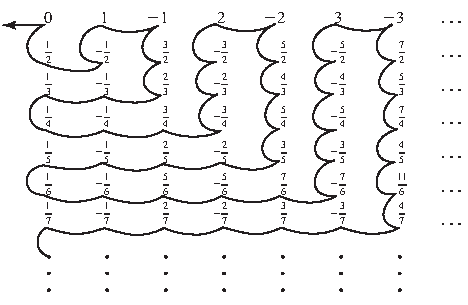
\includegraphics[width=0.642\linewidth,height=.8\textheight,keepaspectratio]{assets/p022_00.pdf}\end{center}
\begin{center}\small\textbf{0.15 Figure}\end{center}
\end{BookFloat}

\noindent downward, and contains all members of \BookInline{\mathbb{Q}.} We have shown a string winding its way through this array. Imagine the fractions to be glued to this string. Taking the beginning of the string and pulling to the left in the direction of the arrow, the string straightens out and all elements of \BookInline{\mathbb{Q}} appear on it in an infinite row as \BookInline{0,\allowbreak \frac{1}{2},\allowbreak - \frac{1}{2},\allowbreak 1,\allowbreak - 1,\allowbreak \frac{3}{2},\allowbreak \cdots.} Thus \BookInline{|\mathbb{Q}|= \aleph _{0}} also.

If the set \BookInline{S= \{x\in \mathbb{R}\mid 0<x<1\}} has cardinality \BookInline{\aleph _{0},\allowbreak } all its elements could be listed as unending decimals in a column extending infinitely downward, perhaps as

\[
\begin{array}{l}
0.3659663426\cdots\\
0.7103958453\cdots\\
0.0358493553\cdots\\
0.9968452214\cdots\\
\qquad\vdots
\end{array}
\]

\noindent We now argue that any such array must omit some number in \BookInline{S.} Surely \BookInline{S} contains a number \BookInline{r} having as its \BookInline{n}th digit after the decimal point a number different from 0, from 9, and from the \BookInline{n}th digit of the \BookInline{n}th number in this list. For example\BookInline{,\allowbreak r} might start \BookInline{.5637\cdots.} The 5 rather than 3 after the decimal point shows \BookInline{r} cannot be the first number in \BookInline{S} listed in the array shown. The 6 rather than 1 in the second digit shows \BookInline{r} cannot be the second number listed, and so on. Because we could make this argument with\textit{ any} \textit{list,} we see that \BookInline{S} has too many elements to be paired with those in \BookInline{\mathbb{Z}^{+ }.} Exercise 15 indicates that \BookInline{\mathbb{R}} has the same number of elements as \BookInline{S.} We just denote the cardinality of \BookInline{\mathbb{R}} by \BookInline{|\mathbb{R}|.} Exercise 19 indicates that there are infinitely many different cardinal numbers even greater than \BookInline{|\mathbb{R}|.}

\BookTextHeading{\textbf{Partitions and Equivalence Relations}  }

\noindent Sets are\textbf{ disjoint} if no two of them share a common element. In Example 0.17 we break up the integers into subsets. Eventually we will see how to define an algebraic structure on these subsets of \BookInline{\mathbb{Z}.} That is, we will be able to “add” two of these subsets to get another subset. We will find that breaking a set into subsets is a valuable tool in a number of settings, so we conclude this section with a brief study of\textit{ partitions} of sets.

\BookLabel{0.16 Definition} A\textbf{ partition} of a set \BookInline{S} is a collection of nonempty subsets of \BookInline{S} such that every element of \BookInline{S} is in exactly one of the subsets. The subsets are the\textbf{ cells} of the partition\BookInline{.}\BookEnd{\blacksquare}

\end{BookBody}

% Source PDF page 23; original printed page 6
\BookSource{23}{6}
\BookNarrativetrue

\begin{BookBody}

When discussing a partition of a set \BookInline{S,\allowbreak } we denote by \BookInline{\overline{x}} the cell containing the element \BookInline{x} of \BookInline{S.}

\BookLabel{0.17 Example} Splitting $\mathbb{Z}$ into the subset of even integers and the subset of odd integers, we obtain a partition of $\mathbb{Z}$ into the two cells listed below.
\[
\begin{aligned}
\overline{0}&=\{\ldots,-8,-6,-4,-2,0,2,4,\ldots\}\\
\overline{1}&=\{\ldots,-7,-5,-3,-1,1,3,5,\ldots\}
\end{aligned}
\]
We can think of $\overline{0}$ as being the integers that are divisible by $2$ and $\overline{1}$ as the integers that when divided by $2$ yield a remainder of $1$. This idea can be used for positive integers other than $2$. For example, we can partition $\mathbb{Z}$ into three cells:
\[
\begin{aligned}
\overline{0}&=\{x\in\mathbb{Z}\mid x\text{ is a multiple of }3\},\\
\overline{1}&=\{x\in\mathbb{Z}\mid\text{the remainder of }x\text{ divided by }3\text{ is }1\},\quad\text{and}\\
\overline{2}&=\{x\in\mathbb{Z}\mid\text{the remainder of }x\text{ divided by }3\text{ is }2\}.
\end{aligned}
\]
Note that when dividing a negative number by $3$, we still obtain a non-negative remainder. For example, $-5\div3$ is $-2$ with remainder $1$, which says that $\overline{-5}=\overline{1}$.

Generalizing, for each $n\in\mathbb{Z}^{+}$, we obtain a partition of $\mathbb{Z}$ consisting of $n$ cells, $\overline{0},\overline{1},\overline{2},\ldots,\overline{n-1}$. For each $0\leq r\leq n-1$, an integer $x$ is in the cell $\overline{r}$ exactly when the remainder of $x\div n$ is $r$. These cells are the \textbf{residue classes modulo} $n$ in $\mathbb{Z}$ and $n$ is called the \textbf{modulus}. We define the set $\mathbb{Z}/n\mathbb{Z}$ as the set containing the cells in this partition. So, for example, $\mathbb{Z}/3\mathbb{Z}=\{\overline{0},\overline{1},\overline{2}\}$. As we can see, $\mathbb{Z}/n\mathbb{Z}=\{\overline{0},\overline{1},\overline{2},\ldots,\overline{n-1}\}$ has exactly $n$ elements.\BookEnd{\blacktriangle}

Each partition of a set \BookInline{S} yields a relation \BookInline{\mathcal{R}} on \BookInline{S} in a natural way: namely, for \BookInline{x,\allowbreak y\in S,\allowbreak } let \BookInline{x\mathcal{R}y} if and only if \BookInline{x} and \BookInline{y} are in the same cell of the partition. In set notation, we would write \BookInline{x\mathcal{R}y} as \BookInline{(x,\allowbreak y)\in \mathcal{R}(}see Definition 0.7). A bit of thought shows that this relation \BookInline{\mathcal{R}} on \BookInline{S} satisfies the three properties of an\textit{ equivalence relation} in the following definition.

\BookLabel{0.18 Definition} An\textbf{ equivalence relation} \BookInline{\mathcal{R}} on a set \BookInline{S} is one that satisfies these three properties for all \BookInline{x,\allowbreak y,\allowbreak z\in S.}

\BookExercise{1.}{(Reflexive\BookInline{)\; x\mathcal{R}x.}}

\BookExercise{2.}{(Symmetric) If \BookInline{x\mathcal{R}y,\allowbreak } then \BookInline{y\mathcal{R}x.}}

\BookExercise{3.}{(Transitive) If \BookInline{x\mathcal{R}y} and \BookInline{y\mathcal{R}z} then \BookInline{x\mathcal{R}z.}} \BookEnd{\blacksquare}

To illustrate why the relation \BookInline{\mathcal{R}} corresponding to a partition of \BookInline{S} satisfies the symmetric condition in the definition, we need only observe that if \BookInline{y} is in the same cell as \BookInline{x} (that is, if \BookInline{x\mathcal{R}y),\allowbreak } then \BookInline{x} is in the same cell as \BookInline{y(}that is\BookInline{,\allowbreak y\mathcal{R}x).} We leave the similar observations to verify the reflexive and transitive properties to Exercise 28.

\BookLabel{0.19 Example} For any nonempty set \BookInline{S,\allowbreak } the equality relation \BookInline{= } defined by the subset \BookInline{\{(x,\allowbreak x)\mid x\in S\}} of \BookInline{S\times S} is an equivalence relation\BookInline{.}\BookEnd{\blacktriangle}

\BookLabel{0.20 Example} \textbf{(Congruence Modulo} \BookInline{n)} Let \BookInline{n\in \mathbb{Z}^{+ }.} The equivalence relation on \BookInline{\mathbb{Z}} corresponding to the partition of \BookInline{\mathbb{Z}} into residue classes modulo \BookInline{n,\allowbreak } discussed in Example 0.17, is\textbf{ con}\textbf{gruence modulo} \BookInline{n.} It is sometimes denoted by \BookInline{\equiv _{n}.} Rather than write \BookInline{a\equiv _{n}b,\allowbreak } we usually write \BookInline{a\equiv b(}mod \BookInline{n),\allowbreak } read, “\BookInline{a} is congruent to \BookInline{b} modulo \BookInline{n.}” For example, we have \BookInline{15\equiv 27(}mod 4) because both 15 and 27 have remainder 3 when divided by \BookInline{4.}\BookEnd{\blacktriangle}

\end{BookBody}

% Source PDF page 24; original printed page 7
\BookSource{24}{7}
\BookNarrativetrue

\begin{BookBody}

\BookLabel{0.21 Example} Let a relation \BookInline{\mathcal{R}} on the set \BookInline{\mathbb{Z}} be defined by \BookInline{n\mathcal{R}m} if and only if \BookInline{nm\geq 0,\allowbreak } and let us determine whether \BookInline{\mathcal{R}} is an equivalence relation.

\textbf{Reflexive} \BookInline{a\mathcal{R}a,\allowbreak } because \BookInline{a^{2}\geq 0} for all \BookInline{a\in \mathbb{Z}.}

\textbf{Symmetric} If \BookInline{a\mathcal{R}b,\allowbreak } then \BookInline{ab\geq 0,\allowbreak } so \BookInline{ba\geq 0} and \BookInline{b\mathcal{R}a.}

\textbf{Transitive} If \BookInline{a\mathcal{R}b} and \BookInline{b\mathcal{R}c,\allowbreak } then \BookInline{ab\geq 0} and \BookInline{bc\geq 0.} Thus \BookInline{ab^{2}c= acb^{2}\geq 0.}

If we knew \BookInline{b^{2}>0,\allowbreak } we could deduce\textit{ ac} \BookInline{\geq 0} whence \BookInline{a\mathcal{R}c.} We have to examine the case \BookInline{b= 0} separately. A moment of thought shows that \BookInline{- 3\mathcal{R}0} and \BookInline{0\mathcal{R}5,\allowbreak } but we do\textit{ not} have \BookInline{- 3\mathcal{R}5.} Thus the relation \BookInline{\mathcal{R}} is not transitive, and hence is not an equivalence relation\BookInline{.}\BookEnd{\blacktriangle}

We observed above that a partition yields a natural equivalence relation. We now show that an equivalence relation on a set yields a natural partition of the set. The theorem that follows states both results for reference.

\BookLabel{0.22 Theorem} \textbf{(Equivalence Relations and Partitions)} Let \BookInline{S} be a nonempty set and let \BookInline{\sim } be an equivalence relation on \BookInline{S.} Then \BookInline{\sim } yields a partition of \BookInline{S,\allowbreak } where

\begin{center}\begin{adjustbox}{max width=\linewidth}\BookInline{\displaystyle \overline{a}= \{x\in S\mid x\sim a\}.}\end{adjustbox}\end{center}

\noindent Also, each partition of \BookInline{S} gives rise to an equivalence relation \BookInline{\sim } on \BookInline{S} where \BookInline{a\sim b} if and only if \BookInline{a} and \BookInline{b} are in the same cell of the partition.

\BookLabel{\textit{Proof}} We must show that the different cells $\overline{a}=\{x\in S\mid x\sim a\}$ for $a\in S$ do give a partition of $S$, so that every element of $S$ is in some cell and so that if $a\in\overline{b}$, then $\overline{a}=\overline{b}$. Let $a\in S$. Then $a\in\overline{a}$ by the reflexive condition (1), so $a$ is in \textit{at least one} cell.

Suppose now that $a\in\overline{b}$. We need to show that $\overline{a}=\overline{b}$ as sets; this will show that $a$ cannot be in more than one cell. There is a standard way to show that two sets are the same:
\begin{center}\textit{Show that each set is a subset of the other.}\end{center}
\noindent We show that $\overline{a}\subseteq\overline{b}$. Let $x\in\overline{a}$. Then $x\sim a$. But $a\in\overline{b}$, so $a\sim b$. Then, by the transitive condition (3), $x\sim b$, so $x\in\overline{b}$. Thus $\overline{a}\subseteq\overline{b}$. Now we show that $\overline{b}\subseteq\overline{a}$. Let $y\in\overline{b}$. Then $y\sim b$. But $a\in\overline{b}$, so $a\sim b$ and, by symmetry (2), $b\sim a$. Then by transitivity (3), $y\sim a$, so $y\in\overline{a}$. Hence $\overline{b}\subseteq\overline{a}$ also, so $\overline{b}=\overline{a}$ and our proof is complete.\BookEnd{\blacklozenge}

Each cell in the partition arising from an equivalence relation is an\textbf{ equivalence} \textbf{class}.

\end{BookBody}

\BookNarrativefalse

\begin{BookBody}

\BookExerciseTitle{0}

\noindent In Exercises 1 through 4, describe the set by listing its elements.

\BookExercise{1.}{\BookInline{\{x\in \mathbb{R}\mid x^{2}= 3\}}}

\BookExercise{2.}{$\{m\in\mathbb{Z}\mid m^2+m=6\}$}

\BookExercise{3.}{\BookInline{\{m\in \mathbb{Z}\mid mn= 60} for some \BookInline{n\in \mathbb{Z}\}}}

\BookExercise{4.}{\BookInline{\{x\in \mathbb{Z}\mid x^{2}- 10x+ 16\leq 0\}}}

\noindent In Exercises 5 through 10, decide whether the object described is indeed a set (is well defined). Give an alternate description of each set.

\BookExercise{5.}{\BookInline{\{n\in \mathbb{Z}^{+ }\mid n} is a large number\BookInline{\}}}

\BookExercise{6.}{\BookInline{\{n\in \mathbb{Z}\mid n^{2}<0\}}}

\BookExercise{7.}{\BookInline{\{n\in \mathbb{Z}\mid 39<n^{3}<57\}}}

\BookExercise{8.}{\BookInline{\{r\in \mathbb{Q}\mid } When \BookInline{r} is multiplied by a sufficiently large power of 2, one obtains a whole number\BookInline{.\}}}

\BookExercise{9.}{\BookInline{\{x\in \mathbb{Z}^{+ }\mid x} is an easy number to factor\BookInline{\}}}

\BookExercise{10.}{\BookInline{\{x\in \mathbb{Q}\mid x} may be written with positive denominator less than \BookInline{4\}}}

\BookExercise{11.}{List the elements in \BookInline{\{a,\allowbreak b,\allowbreak c\}\times \{1,\allowbreak 2,\allowbreak c\}.}}

\end{BookBody}

% Source PDF page 25; original printed page 8
\BookSource{25}{8}
\BookNarrativefalse

\begin{BookBody}

\begin{BookFloat}{00_sets_and_relations-p25-0}
\begin{center}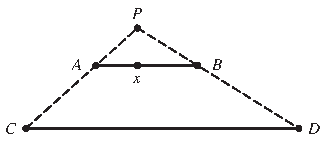
\includegraphics[width=0.445\linewidth,height=.8\textheight,keepaspectratio]{assets/p025_00.pdf}\end{center}
\begin{center}\small\textbf{0.23 Figure}\end{center}
\end{BookFloat}

\BookExercise{12.}{Let \BookInline{A= \{1,\allowbreak 2,\allowbreak 3\}} and \BookInline{B= \{2,\allowbreak 4,\allowbreak 6\}.} For each relation between \BookInline{A} and \BookInline{B} given as a subset of \BookInline{A\times B,\allowbreak } decide whether it is a function mapping \BookInline{A} into \BookInline{B.} If it is a function, decide whether it is one-to-one and whether it is onto \BookInline{B.} \textbf{a}\BookInline{.\{\{1,\allowbreak 2\},\allowbreak \{2,\allowbreak 6\},\allowbreak \{3,\allowbreak 4\}\}} \textbf{b.} [[1,3] and [5,7]] \textbf{c}\BookInline{.\{(1,\allowbreak 6),\allowbreak (1,\allowbreak 2),\allowbreak (1,\allowbreak 4)\}} \textbf{d}\BookInline{.\{\{2,\allowbreak 2\},\allowbreak \{3,\allowbreak 6\},\allowbreak \{1,\allowbreak 6\}\}} \textbf{e}\BookInline{.\{(1,\allowbreak 6),\allowbreak (2,\allowbreak 6),\allowbreak (3,\allowbreak 6)\}} \textbf{f}\BookInline{.\{\{1,\allowbreak 2\},\allowbreak \{2,\allowbreak 6\}\}}}

\BookExercise{13.}{Illustrate geometrically that two line segments \BookInline{AB} and \BookInline{CD} of different lengths have the same number of points by indicating in Fig. 0.23 what point \BookInline{y} of \BookInline{CD} might be paired with point \BookInline{x} of \BookInline{AB.}}

\BookExercise{14.}{Recall that for \BookInline{a,\allowbreak b\in \mathbb{R}} and \BookInline{a<b,\allowbreak } the\textbf{ closed interval} \BookInline{[a,\allowbreak b]} in \BookInline{\mathbb{R}} is defined by \BookInline{[a,\allowbreak b]= \{x\in \mathbb{R}\mid a\leq x\leq } \BookInline{b\}.} Show that the given intervals have the same cardinality by giving a formula for a one-to-one function \BookInline{f} mapping the first interval onto the second. \textbf{a.} [0, 1] and [0, 2] \textbf{b.} [1, 3] and [5, 7] \textbf{c}\BookInline{.[a,\allowbreak b]} and \BookInline{[c,\allowbreak d]}}

\BookExercise{15.}{Show that \BookInline{S= \{x\in \mathbb{R}\mid 0<x<1\}} has the same cardinality as \BookInline{\mathbb{R}.[}\textit{Hint:} Find an elementary function of calculus that maps an interval one-to-one onto \BookInline{\mathbb{R},\allowbreak } and then translate and scale appropriately to make the domain the set \BookInline{S.]}}

\noindent For any set \BookInline{A,\allowbreak } we denote by \BookInline{\mathcal{P}(A)} the collection of all subsets of \BookInline{A.} For example, if \BookInline{A= \{a,\allowbreak b,\allowbreak c,\allowbreak d\},\allowbreak } then \BookInline{\{a,\allowbreak b,\allowbreak d\}\in } \BookInline{\mathcal{P}(A).} The set \BookInline{\mathcal{P}(A)} is the\textbf{ power set} of \BookInline{A.} Exercises 16 through 19 deal with the notion of the power set of a set \BookInline{A.}

\BookExercise{16.}{List the elements of the power set of the given set and give the cardinality of the power set. \textbf{a}\BookInline{.\emptyset } \textbf{b}\BookInline{.\{a\}} \textbf{c}\BookInline{.\{a,\allowbreak b\}} \textbf{d}\BookInline{.\{a,\allowbreak b,\allowbreak c\}}}

\BookExercise{17.}{Let \BookInline{A} be a finite set, and let \BookInline{|A|= s.} Based on the preceding exercise, make a conjecture about the value of \BookInline{|\mathcal{P}(A)|.} Then try to prove your conjecture.}

\BookExercise{18.}{For any set \BookInline{A,\allowbreak } finite or infinite, let \BookInline{B^{A}} be the set of all functions mapping \BookInline{A} into the set \BookInline{B= \{0,\allowbreak 1\}.} Show that the cardinality of \BookInline{B^{A}} is the same as the cardinality of the set \BookInline{\mathcal{P}(A).[}\textit{Hint:} Each element of \BookInline{B^{A}} determines a subset of \BookInline{A} in a natural way.]}

\BookExercise{19.}{Show that the power set of a set \BookInline{A,\allowbreak } finite or infinite, has too many elements to be able to be put in a one-to-one correspondence with \BookInline{A.} Explain why this intuitively means that there are an infinite number of infinite cardinal numbers. [\textit{Hint:} Imagine a one-to-one function \BookInline{\phi } mapping \BookInline{A} into \BookInline{\mathcal{P}(A)} to be given. Show that \BookInline{\phi } cannot be onto \BookInline{\mathcal{P}(A)} by considering, for each \BookInline{x\in A,\allowbreak } whether \BookInline{x\in \phi (x)} and using this idea to define a subset \BookInline{S} of \BookInline{A} that is not in the range of \BookInline{\phi.]} Is\textit{ the set of everything} a logically acceptable concept? Why or why not?}

\BookExercise{20.}{Let \BookInline{A= \{1,\allowbreak 2\}} and let \BookInline{B= \{3,\allowbreak 4,\allowbreak 5\}.}}

\BookExercise{a.}{Illustrate, using \BookInline{A} and \BookInline{B,\allowbreak } why we consider that \BookInline{2+ 3= 5.} Use similar reasoning with sets of your own choice to decide what you would consider to be the value of}

\noindent
\begin{tabular*}{\linewidth}{@{\extracolsep{\fill}}ll@{}}
\textnormal{i.}\quad $3+\aleph_0,$ & \textnormal{ii.}\quad $\aleph_0+\aleph_0.$
\end{tabular*}

\BookExercise{b.}{Illustrate why we consider that \BookInline{2\cdot 3= 6} by plotting the points of \BookInline{A\times B} in the plane \BookInline{\mathbb{R}\times \mathbb{R}.} Use similar reasoning with a figure in the text to decide what you would consider to be the value of \BookInline{\aleph _{0}\cdot \aleph _{0}.}}

\BookExercise{21.}{How many numbers in the interval \BookInline{0\leq x\leq 1} can be expressed in the form.\#\#, where each \# is a digit \BookInline{0,\allowbreak 1,\allowbreak 2,\allowbreak 3,\allowbreak \cdots,\allowbreak 9}? How many are there of the form.\#\#\#\#\#? Following this idea, and Exercise 15, decide what you would consider to be the value of \BookInline{10^{\aleph _{0}}.} How about \BookInline{12^{\aleph _{0}}} and \BookInline{2^{\aleph _{0}}}?}

\end{BookBody}

% Source PDF page 26; original printed page 9
\BookSource{26}{9}
\BookNarrativefalse

\begin{BookBody}

\BookExercise{22.}{Continuing the idea in the preceding exercise and using Exercises 18 and 19, use exponential notation to fill in the three blanks to give a list of five cardinal numbers, each of which is greater than the preceding one.}

\BookInline{\aleph _{0},\allowbreak |\mathbb{R}|,\allowbreak _{- - - },\allowbreak _{- - - },\allowbreak _{- - - }.}

\noindent In Exercises 23 through 27, find the number of different partitions of a set having the given number of elements.

\BookExercise{23.}{1 element}

\BookExercise{24.}{2 elements}

\BookExercise{25.}{3 elements}

\BookExercise{26.}{4 elements}

\BookExercise{27.}{5 elements}

\BookExercise{28.}{Consider a partition of a set $S$. The paragraph following Definition 0.18 explained why the relation $x\mathcal{R}y$ if and only if $x$ and $y$ are in the same cell satisfies the symmetric condition for an equivalence relation. Write similar explanations of why the reflexive and transitive properties are also satisifed.}

\noindent In Exercises 29 through 34, determine whether the given relation is an equivalence relation on the set. Describe the partition arising from each equivalence relation.

\BookExercise{29.}{\BookInline{n\mathcal{R}m} in \BookInline{\mathbb{Z}} if \BookInline{nm>0}}

\BookExercise{30.}{\BookInline{x\mathcal{R}y} in \BookInline{\mathbb{R}} if \BookInline{x\geq y}}

\BookExercise{31.}{\BookInline{x\mathcal{R}y} in \BookInline{\mathbb{Z}^{+ }} if the greatest common divisor of \BookInline{x} and \BookInline{y} is greater than 1}

\BookExercise{32.}{\BookInline{(x_{1},\allowbreak y_{1})\mathcal{R}(x_{2},\allowbreak y_{2})} in \BookInline{\mathbb{R}\times \mathbb{R}} if \BookInline{x_{1}^{2}+ y_{1}^{2}= x_{2}^{2}+ y_{2}^{2}}}

\BookExercise{33.}{\BookInline{n\mathcal{R}m} in \BookInline{\mathbb{Z}^{+ }} if \BookInline{n} and \BookInline{m} have the same number of digits in the usual base ten notation}

\BookExercise{34.}{\BookInline{n\mathcal{R}m} in \BookInline{\mathbb{Z}^{+ }} if \BookInline{n} and \BookInline{m} have the same final digit in the usual base ten notation}

\BookExercise{35.}{Using set notation of the form \BookInline{\{...,\allowbreak } \#, \#, \#\BookInline{,\allowbreak \cdots \},\allowbreak } write the residue classes modulo \BookInline{n} in \BookInline{\mathbb{Z}} as discussed in Example 0.17 for the indicated values of \BookInline{n.} \textbf{a.} 3 \textbf{b.} 4 \textbf{c.} 5}

\BookExercise{36.}{Write each set by listing its elements. \textbf{b}\BookInline{.\mathbb{Z}/4\mathbb{Z}} \textbf{c}\BookInline{.\mathbb{Z}/5\mathbb{Z}} \textbf{a}\BookInline{.\mathbb{Z}/3\mathbb{Z}}}

\BookExercise{37.}{When discussing residue classes, 1 is not well defined until the modulus \BookInline{n} is given. Explain.}

\BookExercise{38.}{Let \BookInline{n\in \mathbb{Z}^{+ }} and let \BookInline{\sim } be defined on \BookInline{\mathbb{Z}} by \BookInline{r\sim s} if and only if \BookInline{r- s} is divisible by \BookInline{n,\allowbreak } that is, if and only if \BookInline{r- s= nq} for some \BookInline{q\in \mathbb{Z}.}}

\BookExercise{a.}{Show that \BookInline{\sim } is an equivalence relation on \BookInline{\mathbb{Z}.}}

\BookExercise{b.}{Show that this \BookInline{\sim } is the equivalence relation,\textit{ congruence modulo} \BookInline{n,\allowbreak } of Example 0.20.}

\BookExercise{39.}{Let \BookInline{n\in \mathbb{Z}^{+ }.} Using the relation from Exercise 38, show that if \BookInline{a_{1}\sim a_{2}} and \BookInline{b_{1}\sim b_{2},\allowbreak } then \BookInline{(a_{1}+ b_{1})} \BookInline{\sim (a_{2}+ b_{2}).}}

\BookExercise{40.}{Let \BookInline{n\in \mathbb{Z}^{+ }.} Using the relation from Exercise 38, show that if \BookInline{a_{1}\sim a_{2}} and \BookInline{b_{1}\sim b_{2},\allowbreak } then \BookInline{(a_{1}b_{1})\sim (a_{2}b_{2}).}}

\BookExercise{41.}{Students often misunderstand the concept of a one-to-one function (mapping). I think I know the reason. You see, a mapping \BookInline{\phi:A\to B} has a\textit{ direction} associated with it, from \BookInline{A} to \BookInline{B.} It seems reasonable to expect a one-to-one mapping simply to be a mapping that carries one point of \BookInline{A} into one point of \BookInline{B,\allowbreak } in the direction indicated by the arrow. But of course,\textit{ every} mapping of \BookInline{A} into \BookInline{B} does this, and Definition 0.12 did not say that at all. With this unfortunate situation in mind, make as good a pedagogical case as you can for calling the functions described in Definition 0.12\textit{ two-to-two functions} instead. (Unfortunately, it is almost impossible to get widely used terminology changed.)}

\end{BookBody}
\ifdefined\BookMaster\let\BookFinish\relax\else\def\BookFinish{\end{document}}\fi\BookFinish

\clearpage
% !TeX program = xelatex
\ifdefined\BookMaster\else
\documentclass[11pt,oneside]{article}
% !TeX program = xelatex
\usepackage[b5paper,left=22mm,right=22mm,top=20mm,bottom=22mm,footskip=11mm]{geometry}
\usepackage{fontspec}
\setmainfont{TeX Gyre Termes}
\setsansfont{TeX Gyre Heros}
\usepackage{amsmath,amssymb,mathtools,amsthm}
\renewcommand{\cdots}{\mathinner{\cdotp\cdotp\cdotp}}
\usepackage{graphicx,adjustbox,array,booktabs,longtable,multirow,enumitem,changepage,needspace}
\usepackage[table]{xcolor}
\usepackage{fancyhdr}
\raggedbottom
\interfootnotelinepenalty=10000
\newcommand{\BookFootnote}[2]{\begingroup\renewcommand{\thefootnote}{\fnsymbol{footnote}}\footnote[#1]{#2}\endgroup}
\newcommand{\BookFootnoteMark}[1]{\begingroup\renewcommand{\thefootnote}{\fnsymbol{footnote}}\footnotemark[#1]\endgroup}
\newcommand{\BookFootnoteText}[2]{\begingroup\renewcommand{\thefootnote}{\fnsymbol{footnote}}\footnotetext[#1]{#2}\endgroup}
\newenvironment{BookFloat}[1]{\par\addvspace{.6\baselineskip}\noindent\def\BookFloatID{#1}\begin{minipage}{\linewidth}\phantomsection\label{bookfloat:#1:start}}{\phantomsection\label{bookfloat:\BookFloatID:end}\end{minipage}\par\addvspace{.6\baselineskip}}

\usepackage[unicode,hidelinks]{hyperref}
\pagestyle{fancy}
\fancyhf{}
\newcommand{\BookFooter}{}
\fancyfoot[L]{\parbox[b]{\dimexpr\textwidth-15mm}{\footnotesize\BookFooter}}
\fancyfoot[R]{\footnotesize\thepage}
\renewcommand{\headrulewidth}{0pt}
\renewcommand{\footrulewidth}{0pt}
\setlength{\parindent}{0pt}
\setlength{\parskip}{0.2em}
\setlength{\emergencystretch}{3em}
\setlist{nosep,leftmargin=1.7em,labelsep=.65em}
\newif\ifBookNarrative
\BookNarrativetrue
\newenvironment{BookBody}{\setlength{\parindent}{0pt}}{}
\newcommand{\BookStatement}[1]{\par\addvspace{.6\baselineskip}\noindent #1\enspace\ignorespaces}
\newcommand{\BookLabel}[1]{\par\addvspace{.6\baselineskip}\needspace{3\baselineskip}\noindent\textbf{#1}\quad\ignorespaces}
\newcommand{\BookHeading}[1]{\par\addvspace{\baselineskip}\needspace{4\baselineskip}\noindent{\large\bfseries #1}\par\medskip}
\newcommand{\BookSubheading}[1]{\par\addvspace{.7\baselineskip}\needspace{3\baselineskip}\noindent{\bfseries #1}\par\smallskip}
\newcommand{\BookTextHeading}[1]{\par\addvspace{.7\baselineskip}\needspace{3\baselineskip}\noindent #1\par\smallskip}
\newcommand{\BookSectionTitle}[2]{\par\addvspace{1.2\baselineskip}\needspace{5\baselineskip}\noindent\colorbox{gray!25}{\sffamily\bfseries\small SECTION #1}\quad{\large\bfseries #2}\par\medskip}
\newcommand{\BookExerciseTitle}[1]{\par\addvspace{\baselineskip}\needspace{4\baselineskip}\noindent{\color{gray}\rule{1.5mm}{1.5mm}}\enspace{\large\bfseries Exercises #1}\par\medskip}
\newcommand{\BookBullet}[1]{\begin{list}{\textbullet}{\setlength{\leftmargin}{1.7em}\setlength{\labelwidth}{1em}\setlength{\labelsep}{.7em}\setlength{\topsep}{0pt}\setlength{\parsep}{0pt}\setlength{\itemsep}{0pt}}\item #1\end{list}}
\newcommand{\BookExercise}[2]{\begin{list}{\textbf{#1}}{\setlength{\leftmargin}{2.2em}\setlength{\labelwidth}{1.5em}\setlength{\labelsep}{.7em}\setlength{\topsep}{.15em}\setlength{\parsep}{0pt}\setlength{\itemsep}{0pt}}\item #2\end{list}}
\newcommand{\BookEnd}[1]{\unskip\nobreak\hfill\ensuremath{#1}}
\newcommand{\BookSource}[2]{\phantomsection\label{sourcepage:#1}} % Source-page anchors, retained through reflow.
\usepackage{multicol}
\usepackage{tikz}
\newcommand{\BookPartEntry}[2]{\par\noindent\makebox[17mm][l]{\bfseries Section #1}#2\par}
\newcommand{\BookPartTitle}[3]{\par\bigskip\noindent\begin{tikzpicture}\node[anchor=north west,inner sep=0pt,outer sep=0pt] (bookpart) at (0,0) {\begin{minipage}{\dimexpr\linewidth-.5pt}\hspace*{26mm}\begin{minipage}[t]{\dimexpr\linewidth-26mm}\begin{adjustbox}{max width=\linewidth}{\fontsize{20}{24}\selectfont\bfseries #2}\end{adjustbox}\par\vspace{6mm}\hrule\vspace{6mm}{\sffamily\footnotesize\setlength{\parskip}{.3em}#3}\vspace{3mm}\end{minipage}\end{minipage}};\path[shade,top color=gray!60,bottom color=white] (0,0) rectangle ([xshift=24mm]bookpart.south west);\node[anchor=north,font=\sffamily\bfseries\small] at (12mm,-2mm) {PART};\node[anchor=north,font=\sffamily\bfseries\Huge] at (12mm,-7mm) {#1};\end{tikzpicture}\par\bigskip}
\newsavebox{\BookMathBox}
\makeatletter
\newcommand{\BookInline}[1]{\leavevmode\hskip0pt\relax\begingroup\in@{\begin}{#1}\ifin@\sbox{\BookMathBox}{\(#1\)}\ifdim\wd\BookMathBox>\dimexpr\linewidth-1em\relax\resizebox{\dimexpr\linewidth-1em\relax}{!}{\usebox{\BookMathBox}}\else\(#1\)\fi\else\in@{\left}{#1}\ifin@\sbox{\BookMathBox}{\(#1\)}\ifdim\wd\BookMathBox>\dimexpr\linewidth-1em\relax\resizebox{\dimexpr\linewidth-1em\relax}{!}{\usebox{\BookMathBox}}\else\(#1\)\fi\else\(#1\)\fi\fi\endgroup\hskip0pt\relax}
\makeatother
\DeclareMathOperator{\Aut}{Aut}
\DeclareMathOperator{\End}{End}
\DeclareMathOperator{\Hom}{Hom}
\DeclareMathOperator{\GF}{GF}
\DeclareMathOperator{\irr}{irr}
\DeclareMathOperator{\lt}{lt}
\DeclareMathOperator{\lp}{lp}
\providecommand{\textcircled}[1]{\textnormal{(#1)}}

\begin{document}
\fi
\renewcommand{\BookFooter}{Section 1 Binary Operations}
\pdfbookmark[0]{Section 1 Binary Operations}{01_binary_operations}
\ifdefined\BookMaster\else\setcounter{page}{11}\fi
% Source PDF page 28; original printed page 11
\BookSource{28}{11}
\BookPartTitle{I}{Groups and Subgroups}{\BookPartEntry{1}{Binary Operations}
\BookPartEntry{2}{Groups}
\BookPartEntry{3}{Abelian Examples}
\BookPartEntry{4}{Nonabelian Examples}
\BookPartEntry{5}{Subgroups}
\BookPartEntry{6}{Cyclic Groups}
\BookPartEntry{7}{Generating Sets and Cayley Digraphs}}

\BookNarrativetrue

\begin{BookBody}

\BookSectionTitle{1}{Binary Operations}

\noindent The transition from elementary school arithmetic to high school algebra involves using letters to represent unknown numbers and studying the basic properties of equations and expressions. The two main binary operations used in high school algebra are addition and multiplication. Abstract algebra takes the next step in abstraction. Not only are the variables unknown, but the actual operations involved may be unknown! We will study sets that have binary operations with properties similar to those of addition and multiplication of numbers. In Part I, our goal will be to develop some of the basic properties of a group. In this section we start our investigation of groups by defining binary operations, naming properties possessed by some binary operations, and giving examples.

\BookTextHeading{\textbf{Definitions and Examples}  }

\noindent The first step in our journey to understand groups is to give a precise mathematical definition of a binary operation that generalizes the familiar addition and multiplication of numbers. Recall that for any set \BookInline{S,\allowbreak } Definition 0.4 defines the set \BookInline{S\times S} to contain all ordered pairs \BookInline{(a,\allowbreak b)} with \BookInline{a,\allowbreak b\in S.}

\BookLabel{1.1 Definition} A\textbf{ binary operation} \BookInline{\ast } on a set \BookInline{S} is a function mapping \BookInline{S\times S} into \BookInline{S.} For each \BookInline{(a,\allowbreak b)\in } \BookInline{S\times S,\allowbreak } we will denote the element \BookInline{\ast ((a,\allowbreak b))} of \BookInline{S} by \BookInline{a\ast b.}\BookEnd{\blacksquare}

Intuitively, we may regard a binary operation \BookInline{\ast } on \BookInline{S} as assigning, to each ordered pair \BookInline{(a,\allowbreak b)} of elements of \BookInline{S,\allowbreak } an element \BookInline{a\ast b} of \BookInline{S.}

\textit{Binary} refers to the fact that we are mapping\textit{ pairs} of elements from \BookInline{S} into \BookInline{S.} We could also define a ternary operation as a function mapping triples of elements of \BookInline{S} to \BookInline{S,\allowbreak } but we will have no need for this type of operation. Throughout this book we will often drop the term binary and use the term operation to mean binary operation.

\BookLabel{1.2 Example} Our usual addition \BookInline{+ } is an operation on the set \BookInline{\mathbb{R}.} Our usual multiplication \BookInline{\cdot } is a different operation on \BookInline{\mathbb{R}.} In this example, we could replace \BookInline{\mathbb{R}} by any of the sets \BookInline{\mathbb{C},\allowbreak \mathbb{Z},\allowbreak } \BookInline{\mathbb{R}^{+ },\allowbreak } or \BookInline{\mathbb{Z}^{+ }.}\BookEnd{\blacktriangle}

\end{BookBody}

% Source PDF page 29; original printed page 12
\BookSource{29}{12}
\BookNarrativetrue

\begin{BookBody}

Note that we require an operation on a set \BookInline{S} to be defined for\textit{ every} ordered pair \BookInline{(a,\allowbreak b)} of elements from \BookInline{S.}

\BookLabel{1.3 Example} Let \BookInline{M(\mathbb{R})} be the set of all matrices\label{bookfootnote:29:2:ref}\BookFootnote{2}{\label{bookfootnote:29:2:text}Most students of abstract algebra have studied linear algebra and are familiar with matrices and matrix operations. For the benefit of those students, examples involving matrices are often given. The reader who is not familiar with matrices can either skip all references to them or turn to the Appendix at the back of the text, where there is a short summary.} with real entries. The usual matrix addition \BookInline{+ } is \textit{not} an operation on this set since \BookInline{A+ B} is not defined for an ordered pair \BookInline{(A,\allowbreak B)} of matrices having different numbers of rows or of columns\BookInline{.}\BookEnd{\blacktriangle}

Sometimes an operation on \BookInline{S} provides an operation on a subset \BookInline{H} of \BookInline{S} also. We make a formal definition.

\BookLabel{1.4 Definition} Let \BookInline{\ast } be an operation on \BookInline{S} and let \BookInline{H} be a subset of \BookInline{S.} The subset \BookInline{H} is\textbf{ closed under} \BookInline{\ast } if for all \BookInline{a,\allowbreak b\in H} we also have \BookInline{a\ast b\in H.} In this case, the operation on \BookInline{H} given by restricting \BookInline{\ast } to \BookInline{H} is the\textbf{ induced operation} of \BookInline{\ast } on \BookInline{H.}\BookEnd{\blacksquare}

By our very definition of an operation \BookInline{\ast } on \BookInline{S,\allowbreak } the set \BookInline{S} is closed under \BookInline{\ast,\allowbreak } but a subset may not be, as the following example shows.

\BookLabel{1.5 Example} Our usual addition \BookInline{+ } on the set \BookInline{\mathbb{R}} of real numbers does not induce an operation on the set \BookInline{\mathbb{R}^{\ast }} of nonzero real numbers because \BookInline{2\in \mathbb{R}^{\ast }} and \BookInline{- 2\in \mathbb{R}^{\ast },\allowbreak } but \BookInline{2+ (- 2)= 0} and \BookInline{0\notin \mathbb{R}^{\ast }.} Thus \BookInline{\mathbb{R}^{\ast }} is not closed under \BookInline{\ast.}\BookEnd{\blacktriangle}

In our text, we will often have occasion to decide whether a subset \BookInline{H} of \BookInline{S} is closed under a binary operation \BookInline{\ast } on \BookInline{S.} To arrive at a correct conclusion,\textit{ we have to know what} \textit{it means for an element to be in} \BookInline{H,\allowbreak } and to use this fact. Students often have trouble here. Be sure you understand the next example.

\BookLabel{1.6 Example} Let \BookInline{+ } and \BookInline{\cdot } be the usual operations of addition and multiplication on the set \BookInline{\mathbb{Z},\allowbreak } and let \BookInline{H= \{n^{2}\mid n\in \mathbb{Z}^{+ }\}.} Determine whether \BookInline{H} is closed under (a) addition and (b) multiplication.

For part (a), we need only observe that \BookInline{1^{2}= 1} and \BookInline{2^{2}= 4} are in \BookInline{H,\allowbreak } but that \BookInline{1+ 4= 5} and \BookInline{5\notin H.} Thus \BookInline{H} is not closed under addition.

For part (b), suppose that \BookInline{r\in H} and \BookInline{s\in H.} Using what it means for \BookInline{r} and \BookInline{s} to be in \BookInline{H,\allowbreak } we see that there must be integers \BookInline{n} and \BookInline{m} in \BookInline{\mathbb{Z}^{+ }} such that \BookInline{r= n^{2}} and \BookInline{s= m^{2}.} Consequently\BookInline{,\allowbreak rs= n^{2}m^{2}= (nm)^{2}.} By the characterization of elements in \BookInline{H} and the fact that \BookInline{nm\in \mathbb{Z}^{+ },\allowbreak } this means that \BookInline{rs\in H,\allowbreak } so \BookInline{H} is closed under multiplication\BookInline{.}\BookEnd{\blacktriangle}

\BookLabel{1.7 Example} Let \BookInline{F} be the set of all real-valued functions \BookInline{f} having as domain the set \BookInline{\mathbb{R}} of real numbers. We are familiar from calculus with the operations \BookInline{+,\allowbreak -,\allowbreak \cdot,\allowbreak } and \BookInline{\circ } on \BookInline{F.} Namely, for each ordered pair \BookInline{(f,\allowbreak g)} of functions in \BookInline{F,\allowbreak } we define for each \BookInline{x\in \mathbb{R}}

\begin{center}\begin{adjustbox}{max width=\linewidth}\BookInline{\displaystyle \begin{aligned}f+ g\;\text{by}\;(f+ g)(x)&= f(x)+ g(x)\;\text{addition}\;,\allowbreak  \\ f- g\;\text{by}\;(f- g)(x)&= f(x)- g(x)\;\text{subtraction}\;,\allowbreak  \\ f\cdot g\;\text{by}\;(f\cdot g)(x)&= f(x)g(x)\;\text{multiplication}\;,\allowbreak \;\text{and}\; \\ f\circ g\;\text{by}\;(f\circ g)(x)&= f(g(x))\;\text{composition}\;.\end{aligned}}\end{adjustbox}\end{center}

\noindent All four of these functions are again real valued with domain \BookInline{\mathbb{R},\allowbreak } so \BookInline{F} is closed under all four operations \BookInline{+,\allowbreak -,\allowbreak \cdot,\allowbreak } and \BookInline{\circ.}\BookEnd{\blacktriangle}

The operations described in the examples above are very familiar to you. In this text, we want to\textit{ abstract} basic structural concepts from our familiar algebra. To empha
% Source PDF page 30; original printed page 13
\BookSource{30}{13}
size this concept of\textit{ abstraction} from the familiar, we should illustrate these structural concepts with unfamiliar examples.

\end{BookBody}

\BookNarrativetrue

\begin{BookBody}

The most important method of describing a particular binary operation \BookInline{\ast } on a given set is to characterize the element \BookInline{a\ast b} assigned to each pair \BookInline{(a,\allowbreak b)} by some property defined in terms of \BookInline{a} and \BookInline{b.}

\BookLabel{1.8 Example} On \BookInline{\mathbb{Z}^{+ },\allowbreak } we define an operation \BookInline{\ast } by \BookInline{a\ast b} equals the smaller of \BookInline{a} and \BookInline{b,\allowbreak } or the common value if \BookInline{a= b.} Thus \BookInline{2\ast 11= 2;15\ast 10= 10;} and \BookInline{3\ast 3= 3.}\BookEnd{\blacktriangle}

\BookLabel{1.9 Example} On \BookInline{\mathbb{Z}^{+ },\allowbreak } we define an operation \BookInline{\ast ^{\prime }} by \BookInline{a\ast ^{\prime }b= a.} Thus \BookInline{2\ast ^{\prime }3= 2;25\ast ^{\prime }10= 25;} and \BookInline{5\ast ^{\prime }5= 5.}\BookEnd{\blacktriangle}

\BookLabel{1.10 Example} On \BookInline{\mathbb{Z}^{+ },\allowbreak } we define an operation \BookInline{\ast ^{\prime \prime }} by \BookInline{a\ast ^{\prime \prime }b= (a\ast b)+ 2,\allowbreak } where \BookInline{\ast } is defined in Example 1.8. Thus \BookInline{4\ast ^{\prime \prime }7= 6;25\ast ^{\prime \prime }9= 11;} and \BookInline{6\ast ^{\prime \prime }6= 8.}\BookEnd{\blacktriangle}

It may seem that these examples are of no importance, but in fact they are used millions of times each day. For example, consider the GPS navigational system installed in most cars and cell phones. It searches alternative driving routes, computes the travel time, and determines which route takes less time. The operation in Example 1.8 is programmed into modern GPS systems and it plays an essential role.

Examples 1.8 and 1.9 were chosen to demonstrate that an operation may or may not depend on the order of the given pair. Thus in Example \BookInline{1.8,\allowbreak a\ast b= b\ast a} for all \BookInline{a,\allowbreak b\in \mathbb{Z}^{+ },\allowbreak } and in Example 1.9 this is not the case, for \BookInline{5\ast ^{\prime }7= 5} but \BookInline{7\ast ^{\prime }5= 7.}

\BookLabel{1.11 Definition} An operation \BookInline{\ast } on a set \BookInline{S} is\textbf{ commutative} if (and only if\BookInline{)\; a\ast b= b\ast a} for all \BookInline{a,\allowbreak b\in S.}\BookEnd{\blacksquare}

As was pointed out in Section 0, it is customary in mathematics to omit the words \textit{and only if} from a definition. Definitions are always understood to be if and only if statements.\textit{ Theorems are not always if and only if statements, and no such convention} \textit{is ever used for theorems}.

Now suppose we wish to consider an expression of the form \BookInline{a\ast b\ast c.} A binary operation \BookInline{\ast } enables us to combine only two elements, and here we have three. The obvious attempts to combine the three elements are to form either \BookInline{(a\ast b)\ast c} or \BookInline{a\ast (b\ast c).} With \BookInline{\ast } defined as in Example \BookInline{1.8,\allowbreak (2\ast 5)\ast 9} is computed by \BookInline{2\ast 5= 2} and then \BookInline{2\ast 9= 2.} Likewise\BookInline{,\allowbreak 2\ast (5\ast 9)} is computed by \BookInline{5\ast 9= 5} and then \BookInline{2\ast 5= 2.} Hence \BookInline{(2\ast 5)\ast 9= 2\ast (5\ast 9),\allowbreak } and it is not hard to see that for this \BookInline{\ast,\allowbreak }

\begin{center}\begin{adjustbox}{max width=\linewidth}\BookInline{\displaystyle (a\ast b)\ast c= a\ast (b\ast c),\allowbreak }\end{adjustbox}\end{center}

\noindent so there is no ambiguity in writing \BookInline{a\ast b\ast c.} But for \BookInline{\ast ^{\prime \prime }} of Example 1.10,

\begin{center}\begin{adjustbox}{max width=\linewidth}\BookInline{\displaystyle (2\ast ^{\prime \prime }5)\ast ^{\prime \prime }9= 4\ast ^{\prime \prime }9= 6,\allowbreak }\end{adjustbox}\end{center}

\noindent while

\begin{center}\begin{adjustbox}{max width=\linewidth}\BookInline{\displaystyle 2\ast ^{\prime \prime }(5\ast ^{\prime \prime }9)= 2\ast ^{\prime \prime }7= 4.}\end{adjustbox}\end{center}

\noindent Thus \BookInline{(a\ast ^{\prime \prime }b)\ast ^{\prime \prime }c} need not equal \BookInline{a\ast ^{\prime \prime }(b\ast ^{\prime \prime }c),\allowbreak } and the expression \BookInline{a\ast ^{\prime \prime }b\ast ^{\prime \prime }c} is ambiguous.

\BookLabel{1.12 Definition} An operation on a set \BookInline{S} is\textbf{ associative} if \BookInline{(a\ast b)\ast c= a\ast (b\ast c)} for all \BookInline{a,\allowbreak b,\allowbreak c\in S.}\BookEnd{\blacksquare}

It can be shown that if \BookInline{\ast } is associative, then longer expressions such as \BookInline{a\ast b\ast } \BookInline{c\ast d} are not ambiguous. Parentheses may be inserted in any fashion for purposes of computation; the final results of two such computations will be the same.

\end{BookBody}

% Source PDF page 31; original printed page 14
\BookSource{31}{14}
\BookNarrativetrue

\begin{BookBody}

Composition of functions mapping \BookInline{\mathbb{R}} into \BookInline{\mathbb{R}} was reviewed in Example 1.7. For any set \BookInline{S} and any functions \BookInline{f} and \BookInline{g} mapping \BookInline{S} into \BookInline{S,\allowbreak } we similarly define the composition \BookInline{f\circ g} of \BookInline{g} followed by \BookInline{f} as the function mapping \BookInline{S} into \BookInline{S} such that \BookInline{(f\circ g)(x)= f(g(x))} for all \BookInline{x\in S.} Some of the most important binary operations we consider are defined using composition of functions. It is important to know that function composition is always associative whenever it is defined.

\BookLabel{1.13 Theorem} \textbf{(Associativity of Composition)} Let \BookInline{S} be a set and let \BookInline{f,\allowbreak g,\allowbreak } and \BookInline{h} be functions mapping \BookInline{S} into \BookInline{S.} Then \BookInline{f\circ (g\circ h)= (f\circ g)\circ h.}

\BookLabel{\textit{Proof}} To show these two functions are equal, we must show that they give the same assignment to each \BookInline{x\in S.} Computing we find that

\begin{center}\begin{adjustbox}{max width=\linewidth}\BookInline{\displaystyle (f\circ (g\circ h))(x)= f((g\circ h)(x))= f(g(h(x)))}\end{adjustbox}\end{center}

\noindent and

\begin{center}\begin{adjustbox}{max width=\linewidth}\BookInline{\displaystyle ((f\circ g)\circ h)(x)= (f\circ g)(h(x))= f(g(h(x))),\allowbreak }\end{adjustbox}\end{center}

\noindent so the same element \BookInline{f(g(h(x)))} of \BookInline{S} is indeed obtained. \BookEnd{\blacklozenge}

As an example of using Theorem 1.13 to save work, recall that it is a fairly painful exercise in summation notation to show that multiplication of \BookInline{n\times n} matrices is an associative operation. If, in a linear algebra course, we first show that there is a one-to-one correspondence between matrices and linear transformations and that multiplication of matrices corresponds to the composition of the linear transformations (functions), we obtain this associativity at once from Theorem 1.13.

There is another property that an operation on a set may have that is of particular importance in algebra. The numbers 0 and 1 play special roles as real numbers because for any real number \BookInline{a,\allowbreak a+ 0= a} and \BookInline{a\times 1= a.} Because of these properties, 0 is called the\textit{ additive identity} in \BookInline{\mathbb{R}} and 1 is called the\textit{ multiplicative identity} in \BookInline{\mathbb{R}.} In general we have the following definition of an identity.

\BookLabel{1.14 Definition} Let \BookInline{S} be a set with binary operation \BookInline{\ast.} If \BookInline{e\in S} has the property that for all \BookInline{a\in S,\allowbreak } \BookInline{a\ast e= e\ast a= a,\allowbreak } then \BookInline{e} is called an\textbf{ identity element for} \BookInline{\ast.}\BookEnd{\blacksquare}

\noindent We included both conditions \BookInline{a\ast e= a} and \BookInline{e\ast a= a} in the definition of an identity because we are not assuming that the operation on \BookInline{S} is commutative. Of course, if the operation is commutative, such as \BookInline{+ } and \BookInline{\times } on the real numbers, then we would only have to check one of the conditions and the other follows from commutativity.

\BookLabel{1.15 Theorem} \textbf{(Uniqueness of Identity)} A set with binary operation \BookInline{\ast } has at most one identity element.

\BookLabel{\textit{Proof}} We need to show that there cannot be two different identity elements. To do this, we assume that both \BookInline{e} and \BookInline{e^{\prime }} are identities and show that \BookInline{e= e^{\prime }.} Consider the element \BookInline{e\ast e^{\prime }.} Since \BookInline{e} is an identity\BookInline{,\allowbreak e\ast e^{\prime }= e^{\prime }.} But \BookInline{e\ast e^{\prime }= e} because \BookInline{e^{\prime }} is also an identity. Therefore \BookInline{e= e^{\prime }.}\BookEnd{\blacklozenge}

\BookLabel{1.16 Example} Continuing with Example 1.7, let \BookInline{F} be the set of all functions mapping the real numbers to the real numbers. We verify that the function defined by \BookInline{\iota (x)= x} is the identity for the operation function composition. Let \BookInline{f\in F.} Then \BookInline{f\circ \iota (x)= f(\iota (x))= f(x)} and \BookInline{\iota \circ f(x)= } \BookInline{\iota (f(x))= f(x).}

The function \BookInline{m(x)= 1} is the identity for the operation function multiplication, \BookInline{a(x)= 0} is the identity for function addition, but function subtraction has no identity element\BookInline{.}\BookEnd{\blacktriangle}

\end{BookBody}

% Source PDF page 32; original printed page 15
\BookSource{32}{15}
\BookNarrativetrue

\begin{BookBody}

The last property that we consider in this section is the existance of inverse elements. For addition, the inverse of a real number \BookInline{a} is \BookInline{- a.} Using multiplication, the inverse of a nonzero real number \BookInline{a} is \BookInline{\frac{1}{a}} We now give the formal definition of an inverse for an element \BookInline{x.}

\BookLabel{1.17 Definition} If \BookInline{\ast } is an operation on the set \BookInline{S} and \BookInline{S} has an identity \BookInline{e,\allowbreak } then for any \BookInline{x\in S,\allowbreak } the inverse of \BookInline{x} is an element \BookInline{x^{\prime }} such that \BookInline{x\ast x^{\prime }= x^{\prime }\ast x= e.}\BookEnd{\blacksquare}

\BookLabel{1.18 Example} Continuing Example 1.16, let \BookInline{F} be the set of functions mapping the real numbers to the real numbers with operation function composition. We have two definitions for the inverse of a function \BookInline{f\in F,\allowbreak } the usual definition of an inverse function and Definition 1.17. The two definitions match since both say that an inverse for \BookInline{f} is a function \BookInline{f^{\prime }} such that \BookInline{f\circ f^{\prime }= f^{\prime }\circ f= \iota.} So \BookInline{f\in F} has an inverse if and only if \BookInline{f} is one-to-one and onto\BookInline{.}\BookEnd{\blacktriangle}

\BookTextHeading{\textbf{Tables}}

\noindent For a finite set, a binary operation on the set can be defined by means of a table in which the elements of the set are listed across the top as heads of columns and at the left side as heads of rows. We always require that the elements of the set be listed as heads across the top in the same order as heads down the left side. The next example illustrates the use of a table to define a binary operation.

\begin{BookFloat}{01_binary_operations-p32-5}
\BookLabel{1.19 Example} Table 1.20 defines the binary operation $\ast$ on $S=\{a,b,c\}$ by the following rule:
\[
\begin{aligned}
&\bigl(i\text{\itshape th entry on the left}\bigr)\ast\bigl(j\text{\itshape th entry on the top}\bigr)\\
&\quad=\bigl(\text{\itshape entry in the }i\text{\itshape th row and }j\text{\itshape th column of the table body}\bigr).
\end{aligned}
\]
\begin{center}
\textbf{1.20 Table}\par\smallskip
\begin{tabular}{c|c|c|c}
$\ast$ & $a$ & $b$ & $c$\\\hline
$a$ & $b$ & $c$ & $b$\\\hline
$b$ & $a$ & $c$ & $b$\\\hline
$c$ & $c$ & $b$ & $a$
\end{tabular}
\end{center}
\noindent Thus $a\ast b=c$ and $b\ast a=a$, so $\ast$ is not commutative.\BookEnd{\blacktriangle}

We can easily see that \textit{a binary operation defined by a table is commutative if and only if the entries in the table are symmetric with respect to the diagonal that starts at the upper left corner of the table and terminates at the lower right corner}.
\end{BookFloat}

\BookLabel{1.21 Example} Complete Table 1.22 so that \BookInline{\ast } is a commutative operation on the set \BookInline{S= \{a,\allowbreak b,\allowbreak c,\allowbreak d\}.}

\BookLabel{\textit{Solution}} From Table 1.22, we see that \BookInline{b\ast a= d.} For \BookInline{\ast } to be commutative, we must have \BookInline{a\ast } \BookInline{b= d} also. Thus we place \BookInline{d} in the appropriate square defining \BookInline{a\ast b,\allowbreak } which is located symmetrically across the diagonal in Table 1.23 from the square defining \BookInline{b\ast a.} We obtain the rest of Table 1.23 in this fashion to give our solution\BookInline{.}\BookEnd{\blacktriangle}

\begin{BookFloat}{01_binary_operations-p32-8}
\begin{center}
\begin{minipage}[t]{0.3852\linewidth}\vspace{0pt}\begin{center}\small\textbf{1.22 Table}\end{center}
\begin{center}\begin{adjustbox}{max width=\linewidth}
\renewcommand{\arraystretch}{1.2}\setlength{\tabcolsep}{5pt}
\begin{tabular}{c|c|c|c|c}
* & \BookInline{a} & \BookInline{b} & \BookInline{c} & \BookInline{d}\\\hline
\BookInline{a} & \BookInline{b} &  &  & \\\hline
\BookInline{b} & \BookInline{d} & \BookInline{a} &  & \\\hline
\BookInline{c} & \BookInline{a} & \BookInline{c} & \BookInline{d} & \\\hline
\BookInline{d} & \BookInline{a} & \BookInline{b} & \BookInline{b} & \BookInline{c}\\
\end{tabular}
\end{adjustbox}\end{center}\end{minipage}\hfill\begin{minipage}[t]{0.3934\linewidth}\vspace{0pt}\begin{center}\small\textbf{1.23 Table}\end{center}
\begin{center}\begin{adjustbox}{max width=\linewidth}
\renewcommand{\arraystretch}{1.2}\setlength{\tabcolsep}{5pt}
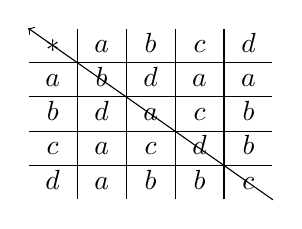
\begin{tikzpicture}\node[inner sep=0pt] (booktable) {
\begin{tabular}{c|c|c|c|c}
\BookInline{\ast } & \BookInline{a} & \BookInline{b} & \BookInline{c} & \BookInline{d}\\\hline
\BookInline{a} & \BookInline{b} & \BookInline{d} & \BookInline{a} & \BookInline{a}\\\hline
\BookInline{b} & \BookInline{d} & \BookInline{a} & \BookInline{c} & \BookInline{b}\\\hline
\BookInline{c} & \BookInline{a} & \BookInline{c} & \BookInline{d} & \BookInline{b}\\\hline
\BookInline{d} & \BookInline{a} & \BookInline{b} & \BookInline{b} & \BookInline{c}\\
\end{tabular}
};\draw[<-] (booktable.north west)--(booktable.south east);\end{tikzpicture}
\end{adjustbox}\end{center}\end{minipage}
\end{center}
\end{BookFloat}

\end{BookBody}

% Source PDF page 33; original printed page 16
\BookSource{33}{16}
\BookNarrativetrue

\begin{BookBody}

\BookLabel{1.24 Example} When an operation has an identity element, it is customary to put the identity first in the list of heads. This makes the first row and the first column match the head row and head column as seen in Table \BookInline{1.25.}\BookEnd{\blacktriangle}

\BookTextHeading{\textbf{Some Words of Warning}  }

\begin{BookFloat}{01_binary_operations-p33-2}
\begin{center}\small\textbf{1.25 Table}\end{center}
\begin{center}\begin{adjustbox}{max width=\linewidth}
\renewcommand{\arraystretch}{1.2}\setlength{\tabcolsep}{5pt}
\begin{tabular}{c|c|c|c|c}
* & \BookInline{e} & \BookInline{a} & \BookInline{b} & \BookInline{c}\\\hline
\BookInline{e} & \BookInline{e} & \BookInline{a} & \BookInline{b} & \BookInline{c}\\\hline
\BookInline{a} & \BookInline{a} & \BookInline{c} & \BookInline{c} & \BookInline{a}\\\hline
\BookInline{b} & \BookInline{b} & \BookInline{a} & \BookInline{e} & \BookInline{c}\\\hline
\BookInline{c} & \BookInline{c} & \BookInline{e} & \BookInline{a} & \BookInline{b}\\
\end{tabular}
\end{adjustbox}\end{center}
\end{BookFloat}

\noindent Classroom experience shows the chaos that may result if a student is given a set and asked to define some binary operation on it. Remember that in an attempt to define a binary operation \BookInline{\ast } on a set S we must be sure that

\BookExercise{1.}{\textit{exactly one element is assigned to each possible ordered pair of elements of} \BookInline{S,\allowbreak }}

\BookExercise{2.}{\textit{for each ordered pair of elements of} \BookInline{S,\allowbreak } \textit{the element assigned to it is again in} \BookInline{S.}}

\noindent Regarding Condition 1, a student will often make an attempt that assigns an element of \BookInline{S} to “most” ordered pairs, but for a few pairs, determines no element. In this event, \BookInline{\ast } is\textbf{ not everywhere defined} on \BookInline{S.} It may also happen that for some pairs, the attempt could assign any of several elements of \BookInline{S,\allowbreak } that is, there is ambiguity. In any case of ambiguity\BookInline{,\allowbreak \ast } is\textbf{ not well defined}. If Condition 2 is violated, then \BookInline{S} is\textbf{ not closed} \textbf{under} \BookInline{\ast.}

\BookLabel{1.26 Example} On which of the sets \BookInline{\mathbb{Q},\allowbreak \mathbb{Q}^{\ast },\allowbreak } and \BookInline{Z^{+ }} does the formula \BookInline{a\ast b= a/b} define an operation? Note that this formula does not make sense in the case that \BookInline{b= 0.} So for example, \BookInline{2\ast 0= 2/0} is not defined, which means Condition 1 is not satisfied. So \BookInline{\ast } is not an operation on \BookInline{\mathbb{Q}.}

If we throw out 0, we do have an operation on \BookInline{\mathbb{Q}^{\ast }} since both Conditions 1 and 2 are satisfied. That is, for any \BookInline{a,\allowbreak b\in \mathbb{Q}^{\ast },\allowbreak a\ast b= a/b} is a nonzero rational number.

The set \BookInline{\mathbb{Z}^{+ }} does not include 0, but there is another issue. For example\BookInline{,\allowbreak 1\ast 2= } \BookInline{1/2\not \in \mathbb{Z}^{+ },\allowbreak } which means that Condition 2 is violated and \BookInline{\ast } is not an operation on \BookInline{\mathbb{Z}^{+ }.}\BookEnd{\blacktriangle}

Following are several illustrations of attempts to define operations on sets. Some of them need some work! The symbol \BookInline{\ast } is used for the attempted operation in all these examples.

\BookLabel{1.27 Example} Let \BookInline{F} be the set of all real-valued functions with domain \BookInline{\mathbb{R}} as in Example 1.7. Suppose we “define” \BookInline{\ast } to give the usual quotient of \BookInline{f} by \BookInline{g,\allowbreak } that is\BookInline{,\allowbreak f\ast g= h,\allowbreak } where \BookInline{h(x)= } \BookInline{f(x)/g(x).} Here Condition 2 is violated, for the functions in \BookInline{F} are defined for\textit{ all} real numbers, and for some \BookInline{g\in F,\allowbreak g(x)} will be zero for some values of \BookInline{x} in \BookInline{\mathbb{R}} and \BookInline{h(x)} would not be defined at those numbers in \BookInline{\mathbb{R}.} For example, if \BookInline{f(x)= } cos \BookInline{x} and \BookInline{g(x)= x^{2},\allowbreak } then \BookInline{h(0)} is undefined, so \BookInline{h\notin F.}\BookEnd{\blacktriangle}

\BookLabel{1.28 Example} Let \BookInline{F} be as in Example 1.27 and let \BookInline{f\ast g= h,\allowbreak } where \BookInline{h} is the function greater than both \BookInline{f} and \BookInline{g.} This “definition” is extremely vague. In the first place, we have not defined what it means for one function to be greater than another. Even if we had, any sensible definition would result in there being many functions greater than both \BookInline{f} and \BookInline{g,\allowbreak } and \BookInline{\ast } would still be\textit{ not well defined}\BookInline{.}\BookEnd{\blacktriangle}

\BookLabel{1.29 Example} Let \BookInline{S} be a set consisting of 20 people, no two of whom are of the same height. Define \BookInline{\ast } by \BookInline{a\ast b= c,\allowbreak } where \BookInline{c} is the tallest person among the 20 in \BookInline{S.} This is a perfectly good binary operation on the set, although not a particularly interesting one\BookInline{.}\BookEnd{\blacktriangle}

\BookLabel{1.30 Example} Let \BookInline{S} be as in Example 1.29 and let \BookInline{a\ast b= c,\allowbreak } where \BookInline{c} is the shortest person in \BookInline{S} who is taller than both \BookInline{a} and \BookInline{b.} This \BookInline{\ast } is\textit{ not everywhere defined,} since if either \BookInline{a} or \BookInline{b} is the tallest person in the set\BookInline{,\allowbreak a\ast b} is not determined\BookInline{.}\BookEnd{\blacktriangle}

\end{BookBody}

% Source PDF page 34; original printed page 17
\BookSource{34}{17}
\BookNarrativefalse

\begin{BookBody}

\BookExerciseTitle{1}

\BookTextHeading{\textbf{Computations}}

\noindent Exercises 1 through 4 concern the binary operation \BookInline{\ast } defined on \BookInline{S= \{a,\allowbreak b,\allowbreak c,\allowbreak d,\allowbreak e\}} by means of Table 1.31.

\BookExercise{1.}{Compute \BookInline{b\ast d,\allowbreak c\ast c,\allowbreak } and \BookInline{[(a\ast c)\ast e]\ast a.}}

\BookExercise{2.}{Compute \BookInline{(a\ast b)\ast c} and \BookInline{a\ast (b\ast c).} Can you say on the basis of this computation whether \BookInline{\ast } is associative?}

\BookExercise{3.}{Compute \BookInline{(b\ast d)\ast c} and \BookInline{b\ast (d\ast c).} Can you say on the basis of this computation whether \BookInline{\ast } is associative?}

\BookExercise{4.}{Is \BookInline{\ast } commutative? Why?}

\BookExercise{5.}{Complete Table 1.32 so as to define a commutative binary operation \BookInline{\ast } on \BookInline{S= \{a,\allowbreak b,\allowbreak c,\allowbreak d\}.}}

\BookExercise{6.}{Table 1.33 can be completed to define an associative binary operation \BookInline{\ast } on \BookInline{S= \{a,\allowbreak b,\allowbreak c,\allowbreak d\}.} Assume this is possible and compute the missing entries. Does \BookInline{S} have an identity element?}

\begin{BookFloat}{01_binary_operations-p34-9}
\begin{center}
\begin{minipage}[t]{0.3135\linewidth}\vspace{0pt}\begin{center}\small\textbf{1.31 Table}\end{center}
\begin{center}\begin{adjustbox}{max width=\linewidth}
\renewcommand{\arraystretch}{1.2}\setlength{\tabcolsep}{5pt}
\begin{tabular}{c|c|c|c|c|c}
* & \BookInline{a} & \BookInline{b} & \BookInline{c} & \BookInline{d} & \BookInline{e}\\\hline
\BookInline{a} & \BookInline{a} & \BookInline{b} & \BookInline{c} & \BookInline{b} & \BookInline{d}\\\hline
\BookInline{b} & \BookInline{b} & \BookInline{c} & \BookInline{a} & \BookInline{e} & \BookInline{c}\\\hline
\BookInline{c} & \BookInline{c} & \BookInline{a} & \BookInline{b} & \BookInline{b} & \BookInline{a}\\\hline
\BookInline{d} & \BookInline{b} & \BookInline{e} & \BookInline{b} & \BookInline{e} & \BookInline{d}\\\hline
\BookInline{e} & \BookInline{d} & \BookInline{b} & \BookInline{a} & \BookInline{d} & \BookInline{c}\\
\end{tabular}
\end{adjustbox}\end{center}\end{minipage}\hfill\begin{minipage}[t]{0.2616\linewidth}\vspace{0pt}\begin{center}\small\textbf{1.32 Table}\end{center}
\begin{center}\begin{adjustbox}{max width=\linewidth}
\renewcommand{\arraystretch}{1.2}\setlength{\tabcolsep}{5pt}
\begin{tabular}{c|c|c|c|c}
* & \BookInline{a} & \BookInline{b} & \BookInline{c} & \BookInline{d}\\\hline
\BookInline{a} & \BookInline{a} & \BookInline{b} & \BookInline{c} & \\\hline
\BookInline{b} & \BookInline{b} & \BookInline{d} &  & \BookInline{c}\\\hline
\BookInline{c} & \BookInline{c} & \BookInline{a} & \BookInline{d} & \BookInline{b}\\\hline
\BookInline{d} & \BookInline{d} &  &  & \BookInline{a}\\
\end{tabular}
\end{adjustbox}\end{center}\end{minipage}\hfill\begin{minipage}[t]{0.2597\linewidth}\vspace{0pt}\begin{center}\small\textbf{1.33 Table}\end{center}
\begin{center}\begin{adjustbox}{max width=\linewidth}
\renewcommand{\arraystretch}{1.2}\setlength{\tabcolsep}{5pt}
\begin{tabular}{c|c|c|c|c}
* & \BookInline{a} & \BookInline{b} & \BookInline{c} & \BookInline{d}\\\hline
\BookInline{a} & \BookInline{a} & \BookInline{b} & \BookInline{c} & \BookInline{d}\\\hline
\BookInline{b} & \BookInline{b} & \BookInline{a} & \BookInline{c} & \BookInline{d}\\\hline
\BookInline{c} & \BookInline{c} & \BookInline{d} & \BookInline{c} & \BookInline{d}\\\hline
\BookInline{d} &  &  &  & \\
\end{tabular}
\end{adjustbox}\end{center}\end{minipage}
\end{center}
\end{BookFloat}

\noindent In Exercises 7 through 11, determine whether the operation \BookInline{\ast } is associative, whether the operation is commutative, and whether the set has an identity element.

\BookExercise{7.}{\BookInline{\ast } defined on \BookInline{\mathbb{Z}} by letting \BookInline{a\ast b= a- b}}

\BookExercise{8.}{\BookInline{\ast } defined on \BookInline{\mathbb{Q}} by letting \BookInline{a\ast b= 2ab+ 3}}

\BookExercise{9.}{\BookInline{\ast } defined on \BookInline{\mathbb{Z}} by letting \BookInline{a\ast b= ab+ a+ b}}

\BookExercise{10.}{\BookInline{\ast } defined on \BookInline{\mathbb{Z}^{+ }} by letting \BookInline{a\ast b= 2^{ab}}}

\BookExercise{11.}{\BookInline{\ast } defined on \BookInline{\mathbb{Z}^{+ }} by letting \BookInline{a\ast b= a^{b}}}

\BookExercise{12.}{Let \BookInline{S} be a set having exactly one element. How many different binary operations can be defined on \BookInline{S}? Answer the question if \BookInline{S} has exactly 2 elements; exactly 3 elements; exactly \BookInline{n} elements.}

\BookExercise{13.}{How many different commutative binary operations can be defined on a set of 2 elements? on a set of 3 elements? on a set of \BookInline{n} elements?}

\BookExercise{14.}{How many different binary operations on a set \BookInline{S} with \BookInline{n} elements have the property that for all \BookInline{x\in S,\allowbreak x\ast x= x}?}

\BookExercise{15.}{How many different binary operations on a set \BookInline{S} with \BookInline{n} elements have an identity element?}

\BookTextHeading{\textbf{Concepts}}

\noindent In Exercises 16 through 19, correct the definition of the italicized term without reference to the text, if correction is needed, so that it is in a form acceptable for publication.

\BookExercise{16.}{A binary operation \BookInline{\ast } is\textit{ commutative} if and only if \BookInline{a\ast b= b\ast a.}}

\BookExercise{17.}{A binary operation \BookInline{\ast } on a set \BookInline{S} is\textit{ associative} if and only if, for all \BookInline{a,\allowbreak b,\allowbreak c\in S,\allowbreak } we have \BookInline{(b\ast c)\ast a= b\ast (c\ast a).}}

\BookExercise{18.}{A subset \BookInline{H} of a set \BookInline{S} is\textit{ closed} under a binary operation \BookInline{\ast } on \BookInline{S} if and only if \BookInline{(a\ast b)\in H} for all \BookInline{a,\allowbreak b\in S.}}

\BookExercise{19.}{An identity in the set \BookInline{S} with operation \BookInline{\ast } is an element \BookInline{e\in S} such that \BookInline{a\ast e= e\ast a= a.}}

\BookExercise{20.}{Is there an example of a set \BookInline{S,\allowbreak } a binary operation on \BookInline{S,\allowbreak } and two different elements \BookInline{e_{1},\allowbreak e_{2}\in S} such that for all \BookInline{a\in S,\allowbreak e_{1}\ast a= a} and \BookInline{a\ast e_{2}= a}? If so, give an example and if not, prove there is not one.}

\end{BookBody}

% Source PDF page 35; original printed page 18
\BookSource{35}{18}
\BookNarrativefalse

\begin{BookBody}

\noindent In Exercises 21 through 26, determine whether the definition of \BookInline{\ast } does give a binary operation on the set. In the event that \BookInline{\ast } is not a binary operation, state whether Condition 1, Condition 2, or both conditions regarding defining binary operations are violated.

\BookExercise{21.}{On \BookInline{\mathbb{Z}^{+ },\allowbreak } define \BookInline{a\ast b= b^{a}.}}

\BookExercise{22.}{On \BookInline{\mathbb{R}^{+ },\allowbreak } define \BookInline{\ast } by letting \BookInline{a\ast b= 2a- b.}}

\BookExercise{23.}{On \BookInline{\mathbb{R}^{+ },\allowbreak } define \BookInline{\ast } by \BookInline{a\ast b} to be the minimum of \BookInline{a} and \BookInline{b- 1} if they are different and their common value if they are the same.}

\BookExercise{24.}{On \BookInline{\mathbb{R},\allowbreak } define \BookInline{a\ast b} to be the number \BookInline{c} so that \BookInline{c^{b}= a.}}

\BookExercise{25.}{On \BookInline{\mathbb{Z}^{+ },\allowbreak } define \BookInline{\ast } by letting \BookInline{a\ast b= c,\allowbreak } where \BookInline{c} is at least 5 more than \BookInline{a+ b.}}

\BookExercise{26.}{On \BookInline{\mathbb{Z}^{+ },\allowbreak } define \BookInline{\ast } by letting \BookInline{a\ast b= c,\allowbreak } where \BookInline{c} is the largest integer less than the product of \BookInline{a} and \BookInline{b.}}

\BookExercise{27.}{Let $H$ be the subset of $M_2(\mathbb{R})$ consisting of all matrices of the form $\begin{bmatrix}a&-b\\b&a\end{bmatrix}$ for $a,b\in\mathbb{R}$. Is $H$ closed under \textbf{a.} matrix addition? \textbf{b.} matrix multiplication?}

\BookExercise{28.}{Determine whether each of the following is true or false.}

\BookExercise{a.}{If \BookInline{\ast } is any binary operation on any set \BookInline{S,\allowbreak } then \BookInline{a\ast a= a} for all \BookInline{a\in S.}}

\BookExercise{b.}{If \BookInline{\ast } is any commutative binary operation on any set \BookInline{S,\allowbreak } then \BookInline{a\ast (b\ast c)= (b\ast c)\ast a} for all \BookInline{a,\allowbreak b,\allowbreak c\in S.}}

\BookExercise{c.}{If \BookInline{\ast } is any associative binary operation on any set \BookInline{S,\allowbreak } then \BookInline{a\ast (b\ast c)= (b\ast c)\ast a} for all \BookInline{a,\allowbreak b,\allowbreak c\in S.}}

\BookExercise{d.}{The only binary operations of any importance are those defined on sets of numbers.}

\BookExercise{e.}{A binary operation \BookInline{\ast } on a set \BookInline{S} is commutative if there exist \BookInline{a,\allowbreak b\in S} such that \BookInline{a\ast b= b\ast a.}}

\BookExercise{f.}{Every binary operation defined on a set having exactly one element is both commutative and associative.}

\BookExercise{g.}{A binary operation on a set \BookInline{S} assigns at least one element of \BookInline{S} to each ordered pair of elements of \BookInline{S.}}

\BookExercise{h.}{A binary operation on a set \BookInline{S} assigns at most one element of \BookInline{S} to each ordered pair of elements of \BookInline{S.}}

\BookExercise{i.}{A binary operation on a set \BookInline{S} assigns exactly one element of \BookInline{S} to each ordered pair of elements of \BookInline{S.}}

\BookExercise{j.}{A binary operation on a set \BookInline{S} may assign more than one element of \BookInline{S} to some ordered pair of elements of \BookInline{S.}}

\BookExercise{k.}{For any binary operation \BookInline{\ast } on the set \BookInline{S,\allowbreak } if \BookInline{a,\allowbreak b,\allowbreak c\in S} and \BookInline{a\ast b= a\ast c,\allowbreak } then \BookInline{b= c.}}

\BookExercise{l.}{For any binary operation \BookInline{\ast } on the set \BookInline{S,\allowbreak } there is an element \BookInline{e\in S} such that for all \BookInline{x\in S,\allowbreak x\ast e= x.}}

\BookExercise{m.}{There is an operation on the set \BookInline{S= \{e_{1},\allowbreak e_{2},\allowbreak a\}} so that for all \BookInline{x\in S,\allowbreak e_{1}\ast x= e_{2}\ast x= x.}}

\BookExercise{n.}{Identity elements are always called \BookInline{e.}}

\BookExercise{29.}{Give a set different from any of those described in the examples of the text and not a set of numbers. Define two different binary operations \BookInline{\ast } and \BookInline{\ast ^{\prime }} on this set. Be sure that your set is\textit{ well defined}.}

\BookTextHeading{\textbf{Theory}}

\BookExercise{30.}{Prove that if \BookInline{\ast } is an associative and commutative binary operation on a set \BookInline{S,\allowbreak } then}

\begin{center}\begin{adjustbox}{max width=\linewidth}\BookInline{\displaystyle (a\ast b)\ast (c\ast d)= [(d\ast c)\ast a]\ast b}\end{adjustbox}\end{center}

\noindent for all \BookInline{a,\allowbreak b,\allowbreak c,\allowbreak d\in S.} Assume the associative law only for triples as in the definition, that is, assume only

\begin{center}\begin{adjustbox}{max width=\linewidth}\BookInline{\displaystyle (x\ast y)\ast z= x\ast (y\ast z)}\end{adjustbox}\end{center}

\noindent for all \BookInline{x,\allowbreak y,\allowbreak z\in S.}

\noindent In Exercises 31 and 32, either prove the statement or give a counterexample.

\BookExercise{31.}{Every binary operation on a set consisting of a single element is both commutative and associative.}

\BookExercise{32.}{Every commutative binary operation on a set having just two elements is associative.}

\noindent Let \BookInline{F} be the set of all real-valued functions having as domain the set \BookInline{\mathbb{R}} of all real numbers. Example 1.7 defined the binary operations \BookInline{+,\allowbreak -,\allowbreak \cdot,\allowbreak } and \BookInline{\circ } on \BookInline{F.} In Exercises 33 through 41, either prove the given statement or give a counterexample.

\BookExercise{33.}{Function addition \BookInline{+ } on \BookInline{F} is associative.}

\BookExercise{34.}{Function subtraction \BookInline{- } on \BookInline{F} is commutative.}

\end{BookBody}

% Continuation on source PDF page 36, preceding Section 2
\BookNarrativefalse

\begin{BookBody}

\BookExercise{35.}{Function subtraction \BookInline{- } on \BookInline{F} is associative.}

\BookExercise{36.}{Under function subtraction \BookInline{- F} has an identity.}

\BookExercise{37.}{Under function multiplication \BookInline{\cdot F} has an identity.}

\BookExercise{38.}{Function multiplication \BookInline{\cdot } on \BookInline{F} is commutative.}

\BookExercise{39.}{Function multiplication \BookInline{\cdot } on \BookInline{F} is associative.}

\BookExercise{40.}{Function composition \BookInline{\circ } on \BookInline{F} is commutative.}

\BookExercise{41.}{If \BookInline{\ast } and \BookInline{\ast ^{\prime }} are any two binary operations on a set \BookInline{S,\allowbreak } then}

\begin{center}\begin{adjustbox}{max width=\linewidth}\BookInline{\displaystyle a\ast (b\ast ^{\prime }c)= (a\ast b)\ast ^{\prime }(a\ast c)\;\text{for all}\;a,\allowbreak b,\allowbreak c\in S.}\end{adjustbox}\end{center}

\BookExercise{42.}{Suppose that \BookInline{\ast } is an\textit{ associative binary} operation on a set \BookInline{S.} Let \BookInline{H= \{a\in S\mid a\ast x= x\ast a} for all \BookInline{x\in S\}.} Show that \BookInline{H} is closed under \BookInline{\ast.(}We think of \BookInline{H} as consisting of all elements of \BookInline{S} that\textit{ commute} with every element in \BookInline{S.)}}

\BookExercise{43.}{Suppose that \BookInline{\ast } is an associative and commutative binary operation on a set \BookInline{S.} Show that \BookInline{H= \{a\in S\mid a\ast a= } \BookInline{a\}} is closed under \BookInline{\ast.(}The elements of \BookInline{H} are\textbf{ idempotents} of the binary operation \BookInline{\ast.)}}

\BookExercise{44.}{Let \BookInline{S} be a set and let \BookInline{\ast } be a binary operation on \BookInline{S} satisfying the two laws}

\BookBullet{\BookInline{x\ast x= x} for all \BookInline{s\in S,\allowbreak } and}

\BookBullet{\BookInline{(x\ast y)\ast z= (y\ast z)\ast x} for all \BookInline{x,\allowbreak y,\allowbreak z\in S.}}

Show that \BookInline{\ast } is associative and commutative. (This is problem B-1 on the 1971 Putnam Competition.)

\end{BookBody}
\ifdefined\BookMaster\let\BookFinish\relax\else\def\BookFinish{\end{document}}\fi\BookFinish

\clearpage
% !TeX program = xelatex
\ifdefined\BookMaster\else
\documentclass[11pt,oneside]{article}
% !TeX program = xelatex
\usepackage[b5paper,left=22mm,right=22mm,top=20mm,bottom=22mm,footskip=11mm]{geometry}
\usepackage{fontspec}
\setmainfont{TeX Gyre Termes}
\setsansfont{TeX Gyre Heros}
\usepackage{amsmath,amssymb,mathtools,amsthm}
\renewcommand{\cdots}{\mathinner{\cdotp\cdotp\cdotp}}
\usepackage{graphicx,adjustbox,array,booktabs,longtable,multirow,enumitem,changepage,needspace}
\usepackage[table]{xcolor}
\usepackage{fancyhdr}
\raggedbottom
\interfootnotelinepenalty=10000
\newcommand{\BookFootnote}[2]{\begingroup\renewcommand{\thefootnote}{\fnsymbol{footnote}}\footnote[#1]{#2}\endgroup}
\newcommand{\BookFootnoteMark}[1]{\begingroup\renewcommand{\thefootnote}{\fnsymbol{footnote}}\footnotemark[#1]\endgroup}
\newcommand{\BookFootnoteText}[2]{\begingroup\renewcommand{\thefootnote}{\fnsymbol{footnote}}\footnotetext[#1]{#2}\endgroup}
\newenvironment{BookFloat}[1]{\par\addvspace{.6\baselineskip}\noindent\def\BookFloatID{#1}\begin{minipage}{\linewidth}\phantomsection\label{bookfloat:#1:start}}{\phantomsection\label{bookfloat:\BookFloatID:end}\end{minipage}\par\addvspace{.6\baselineskip}}

\usepackage[unicode,hidelinks]{hyperref}
\pagestyle{fancy}
\fancyhf{}
\newcommand{\BookFooter}{}
\fancyfoot[L]{\parbox[b]{\dimexpr\textwidth-15mm}{\footnotesize\BookFooter}}
\fancyfoot[R]{\footnotesize\thepage}
\renewcommand{\headrulewidth}{0pt}
\renewcommand{\footrulewidth}{0pt}
\setlength{\parindent}{0pt}
\setlength{\parskip}{0.2em}
\setlength{\emergencystretch}{3em}
\setlist{nosep,leftmargin=1.7em,labelsep=.65em}
\newif\ifBookNarrative
\BookNarrativetrue
\newenvironment{BookBody}{\setlength{\parindent}{0pt}}{}
\newcommand{\BookStatement}[1]{\par\addvspace{.6\baselineskip}\noindent #1\enspace\ignorespaces}
\newcommand{\BookLabel}[1]{\par\addvspace{.6\baselineskip}\needspace{3\baselineskip}\noindent\textbf{#1}\quad\ignorespaces}
\newcommand{\BookHeading}[1]{\par\addvspace{\baselineskip}\needspace{4\baselineskip}\noindent{\large\bfseries #1}\par\medskip}
\newcommand{\BookSubheading}[1]{\par\addvspace{.7\baselineskip}\needspace{3\baselineskip}\noindent{\bfseries #1}\par\smallskip}
\newcommand{\BookTextHeading}[1]{\par\addvspace{.7\baselineskip}\needspace{3\baselineskip}\noindent #1\par\smallskip}
\newcommand{\BookSectionTitle}[2]{\par\addvspace{1.2\baselineskip}\needspace{5\baselineskip}\noindent\colorbox{gray!25}{\sffamily\bfseries\small SECTION #1}\quad{\large\bfseries #2}\par\medskip}
\newcommand{\BookExerciseTitle}[1]{\par\addvspace{\baselineskip}\needspace{4\baselineskip}\noindent{\color{gray}\rule{1.5mm}{1.5mm}}\enspace{\large\bfseries Exercises #1}\par\medskip}
\newcommand{\BookBullet}[1]{\begin{list}{\textbullet}{\setlength{\leftmargin}{1.7em}\setlength{\labelwidth}{1em}\setlength{\labelsep}{.7em}\setlength{\topsep}{0pt}\setlength{\parsep}{0pt}\setlength{\itemsep}{0pt}}\item #1\end{list}}
\newcommand{\BookExercise}[2]{\begin{list}{\textbf{#1}}{\setlength{\leftmargin}{2.2em}\setlength{\labelwidth}{1.5em}\setlength{\labelsep}{.7em}\setlength{\topsep}{.15em}\setlength{\parsep}{0pt}\setlength{\itemsep}{0pt}}\item #2\end{list}}
\newcommand{\BookEnd}[1]{\unskip\nobreak\hfill\ensuremath{#1}}
\newcommand{\BookSource}[2]{\phantomsection\label{sourcepage:#1}} % Source-page anchors, retained through reflow.
\usepackage{multicol}
\usepackage{tikz}
\newcommand{\BookPartEntry}[2]{\par\noindent\makebox[17mm][l]{\bfseries Section #1}#2\par}
\newcommand{\BookPartTitle}[3]{\par\bigskip\noindent\begin{tikzpicture}\node[anchor=north west,inner sep=0pt,outer sep=0pt] (bookpart) at (0,0) {\begin{minipage}{\dimexpr\linewidth-.5pt}\hspace*{26mm}\begin{minipage}[t]{\dimexpr\linewidth-26mm}\begin{adjustbox}{max width=\linewidth}{\fontsize{20}{24}\selectfont\bfseries #2}\end{adjustbox}\par\vspace{6mm}\hrule\vspace{6mm}{\sffamily\footnotesize\setlength{\parskip}{.3em}#3}\vspace{3mm}\end{minipage}\end{minipage}};\path[shade,top color=gray!60,bottom color=white] (0,0) rectangle ([xshift=24mm]bookpart.south west);\node[anchor=north,font=\sffamily\bfseries\small] at (12mm,-2mm) {PART};\node[anchor=north,font=\sffamily\bfseries\Huge] at (12mm,-7mm) {#1};\end{tikzpicture}\par\bigskip}
\newsavebox{\BookMathBox}
\makeatletter
\newcommand{\BookInline}[1]{\leavevmode\hskip0pt\relax\begingroup\in@{\begin}{#1}\ifin@\sbox{\BookMathBox}{\(#1\)}\ifdim\wd\BookMathBox>\dimexpr\linewidth-1em\relax\resizebox{\dimexpr\linewidth-1em\relax}{!}{\usebox{\BookMathBox}}\else\(#1\)\fi\else\in@{\left}{#1}\ifin@\sbox{\BookMathBox}{\(#1\)}\ifdim\wd\BookMathBox>\dimexpr\linewidth-1em\relax\resizebox{\dimexpr\linewidth-1em\relax}{!}{\usebox{\BookMathBox}}\else\(#1\)\fi\else\(#1\)\fi\fi\endgroup\hskip0pt\relax}
\makeatother
\DeclareMathOperator{\Aut}{Aut}
\DeclareMathOperator{\End}{End}
\DeclareMathOperator{\Hom}{Hom}
\DeclareMathOperator{\GF}{GF}
\DeclareMathOperator{\irr}{irr}
\DeclareMathOperator{\lt}{lt}
\DeclareMathOperator{\lp}{lp}
\providecommand{\textcircled}[1]{\textnormal{(#1)}}

\begin{document}
\fi
\renewcommand{\BookFooter}{Section 2 Groups}
\pdfbookmark[0]{Section 2 Groups}{02_groups}
\ifdefined\BookMaster\else\setcounter{page}{19}\fi
% Source PDF page 36; original printed page 19
\BookSource{36}{19}
\BookNarrativetrue

\begin{BookBody}

\BookSectionTitle{2}{Groups}

\noindent In high school algebra, one of the key objectives is to learn how to solve equations. Even before learning algebra, students in elementary school are given problems like \BookInline{5+ \square = 2} or \BookInline{2\times \square = 3,\allowbreak } which become \BookInline{5+ x= 2} and \BookInline{2x= 3} in high school algebra. Let us closely examine the steps we use to solve these equations:

\[
\begin{aligned}
5+x &= 2, &&\text{given,}\\
-5+(5+x) &= -5+2, &&\text{adding }-5,\\
(-5+5)+x &= -5+2, &&\text{associative law,}\\
0+x &= -5+2, &&\text{computing }-5+5,\\
x &= -5+2, &&\text{property of }0,\\
x &= -3, &&\text{computing }-5+2.
\end{aligned}
\]

\noindent Strictly speaking, we have not shown here that \BookInline{- 3} is a solution, but rather that it is the only possibility for a solution. To show that \BookInline{- 3} is a solution, one merely computes \BookInline{5+ (- 3).} A similar analysis could be made for the equation \BookInline{2x= 3} in the rational numbers with the operation of multiplication:

\[
\begin{aligned}
2x &= 3, &&\text{given,}\\
\frac{1}{2}(2x) &= \frac{1}{2}(3), &&\text{multiplying by }\frac{1}{2},\\
\left(\frac{1}{2}\cdot2\right)x &= \frac{1}{2}3, &&\text{associative law,}\\
1\cdot x &= \frac{1}{2}3, &&\text{computing }\frac{1}{2}2,\\
x &= \frac{1}{2}3, &&\text{property of }1,\\
x &= \frac{3}{2}, &&\text{computing }\frac{1}{2}3.
\end{aligned}
\]

Now suppose that we have a set with a binary operation \BookInline{\ast.} What properties does the operation need to have in order to solve an equation of the form \BookInline{a\ast x= b} where \BookInline{a} and \BookInline{b} are fixed elements of \BookInline{S}? Both equations \BookInline{5+ x= 2} and \BookInline{2x= 3} have this form; the 
% Source PDF page 37; original printed page 20
\BookSource{37}{20}
first uses the operation \BookInline{+,\allowbreak } and the second uses the operation \BookInline{\times.} By examining the steps used we can see what properties of the operation \BookInline{\ast } are required as summarized in the table below.

\end{BookBody}

\BookNarrativetrue

\begin{BookBody}

\begin{BookFloat}{02_groups-p37-1}
\begin{center}
\begin{adjustbox}{max width=\linewidth}
\renewcommand{\arraystretch}{1.35}\setlength{\tabcolsep}{5pt}
\begin{tabular}{r|c|c}
Property & $+$ & $\times$\\\hline
Associative Property & $-5+(5+x)=(-5+5)+x$ & $\frac12(2x)=\left(\frac12\cdot2\right)x$\\
Identity Element & $0:0+x=x$ & $1:1\cdot x=x$\\
Inverse Element & $-5:-5+5=0$ & $\frac12:\frac12\cdot2=1$
\end{tabular}\end{adjustbox}\end{center}
\end{BookFloat}

If \BookInline{S} is a set with an operation \BookInline{\ast } satisfying these three properties, then an equation of the form \BookInline{a\ast x= b} could be solved for \BookInline{x} using exactly the same steps used to solve \BookInline{5+ x= 2} or \BookInline{2x= 3.} These three essential properties are all that is required in order to have a group. We are now ready to present the precise definition.

\BookTextHeading{\textbf{Definition and Examples}  }

\BookLabel{2.1 Definition} A\textbf{ group} \BookInline{\langle G,\allowbreak \ast \rangle } is a set \BookInline{G,\allowbreak } closed under a binary operation \BookInline{\ast,\allowbreak } such that the following axioms are satisfied:

\BookInline{\mathcal{G}_{1}:} For all \BookInline{a,\allowbreak b,\allowbreak c\in G,\allowbreak } we have

\begin{center}\begin{adjustbox}{max width=\linewidth}\BookInline{\displaystyle (a\ast b)\ast c= a\ast (b\ast c).\;\text{associativity of}\;\ast}\end{adjustbox}\end{center}

\BookInline{\mathcal{G}_{2}:} There is an element \BookInline{e} in \BookInline{G} such that for all \BookInline{x\in G,\allowbreak }

\begin{center}\begin{adjustbox}{max width=\linewidth}\BookInline{\displaystyle e\ast x= x\ast e= x.\;\text{identity element}\;e\;\text{for}\;\ast}\end{adjustbox}\end{center}

\BookInline{\mathcal{G}_{3}:} Corresponding to each \BookInline{a\in G,\allowbreak } there is an element \BookInline{a^{\prime }} in \BookInline{G} such that

\begin{center}\begin{adjustbox}{max width=\linewidth}\BookInline{\displaystyle a\ast a^{\prime }= a^{\prime }\ast a= e.\;\text{inverse}\;a^{\prime }\;\text{of}\;a}\end{adjustbox}\end{center} \BookEnd{\blacksquare}

\BookLabel{2.2 Example} \BookInline{\langle \mathbb{R},\allowbreak + \rangle } is a group with identity element 0 and the inverse of any real number \BookInline{a} is \BookInline{- a.} However\BookInline{,\allowbreak \langle \mathbb{R},\allowbreak \cdot \rangle } is not a group since 0 has no multiplicative inverse. We were still able to solve \BookInline{2x= 3} in the example above because \BookInline{\langle \mathbb{R}^{\ast },\allowbreak \cdot \rangle } is a group since multiplication of real numbers is associative, 1 is an identity, and every real number except 0 has an inverse\BookInline{.}\BookEnd{\blacktriangle}

It is often convenient to say that \BookInline{G} is a group under the operation \BookInline{\ast } rather than write \BookInline{\langle G,\allowbreak \ast \rangle } is a group. At times, there is only one obvious operation that makes \BookInline{\langle G,\allowbreak \ast \rangle } a group. In this case, we may abuse notation and say that \BookInline{G} is a group. For example, if we say that \BookInline{\mathbb{R}} is a group, we mean that \BookInline{\mathbb{R}} is a group under addition.

\BookLabel{2.3 Definition} A group \BookInline{G} is\textbf{ abelian} if its binary operation is commutative. \BookEnd{\blacksquare}

Let us give some examples of some sets with binary operations that give groups and also of some that do not give groups.

\BookLabel{2.4 Example} The set \BookInline{\mathbb{Z}^{+ }} under addition is\textit{ not} a group. There is no identity element for \BookInline{+ } in \BookInline{\mathbb{Z}^{+ }.}\BookEnd{\blacktriangle}

\BookLabel{2.5 Example} The set of all nonnegative integers (including 0) under addition is still\textit{ not} a group. There is an identity element 0, but no inverse for \BookInline{2.}\BookEnd{\blacktriangle}

\end{BookBody}

% Source PDF page 38; original printed page 21
\BookSource{38}{21}
\BookNarrativefalse

\begin{BookBody}

\BookTextHeading{\ensuremath{\blacksquare} \textbf{HISTORICAL NOTE}  }

\noindent There are three historical roots of the development of abstract group theory evident in the mathematical literature of the nineteenth century: the theory of algebraic equations, number theory, and geometry. All three of these areas used group-theoretic methods of reasoning, although the methods were considerably more explicit in the first area than in the other two.

\noindent One of the central themes of geometry in the nineteenth century was the search for invariants under various types of geometric transformations. Gradually attention became focused on the transformations themselves, which in many cases can be thought of as elements of groups.

\noindent In number theory, already in the eighteenth century Leonhard Euler had considered the remainders on division of powers \BookInline{a^{n}} by a fixed prime \BookInline{p.} These remainders have “group” properties.

Similarly, Carl F. Gauss, in his\textit{ Disquisitiones} \textit{Arithmeticae} (1800), dealt extensively with quadratic forms \BookInline{ax^{2}+ 2bxy+ cy^{2},\allowbreak } and in particular showed that equivalence classes of these forms under composition possessed what amounted to group properties.

Finally, the theory of algebraic equations provided the most explicit prefiguring of the group concept. Joseph-Louis Lagrange (1736–1813) in fact initiated the study of permutations of the roots of an equation as a tool for solving it. These permutations, of course, were ultimately considered as elements of a group.

It was Walther von Dyck (1856–1934) and Heinrich Weber (1842–1913) who in 1882 were able independently to combine the three historical roots and give clear definitions of the notion of an abstract group.

\BookLabel{2.6 Example} The familiar additive properties of integers and of rational, real, and complex numbers show that \BookInline{\mathbb{Z},\allowbreak \mathbb{Q},\allowbreak \mathbb{R},\allowbreak } and \BookInline{\mathbb{C}} under addition are abelian groups\BookInline{.}\BookEnd{\blacktriangle}

\BookLabel{2.7 Example} The set \BookInline{\mathbb{Z}^{+ }} under multiplication is\textit{ not} a group. There is an identity 1, but no inverse of \BookInline{3.}\BookEnd{\blacktriangle}

\BookTextHeading{\ensuremath{\blacksquare} \textbf{HISTORICAL NOTE}  }

\noindent Commutative groups are called\textit{ abelian} in honor of the Norwegian mathematician Niels Henrik Abel (1802–1829). Abel was interested in the question of solvability of polynomial equations. In a paper written in 1828, he proved that if all the roots of such an equation can be expressed as rational functions \BookInline{f,\allowbreak g,\allowbreak...,\allowbreak h} of one of them, say \BookInline{x,\allowbreak } and if for any two of these roots\BookInline{,\allowbreak f(x)} and \BookInline{g(x),\allowbreak } the relation \BookInline{f(g(x))= g(f(x))} always holds, then the equation is solvable by radicals. Abel showed that each of these functions in fact permutes the roots of the equation; hence, these functions are elements of the group of permutations of the roots. It was this property of commutativity in these permutation groups associated with solvable equations that led Camille Jordan in his 1870 treatise on algebra to name such groups\textit{ abelian;} the name since then has been applied to commutative groups in general.

Abel was attracted to mathematics as a teenager and soon surpassed all his teachers in Norway. He finally received a government travel grant to study elsewhere in 1825 and proceeded to Berlin, where he befriended August Crelle, the founder of the most influential German mathematical journal. Abel contributed numerous papers to Crelle’s \BookInline{Jour}\BookInline{nal} during the next several years, including many in the field of elliptic functions, whose theory he created virtually single-handedly. Abel returned to Norway in 1827 with no position and an abundance of debts. He nevertheless continued to write brilliant papers, but died of tuberculosis at the age of 26, two days before Crelle succeeded in finding a university position for him in Berlin.

\end{BookBody}

% Source PDF page 39; original printed page 22
\BookSource{39}{22}
\BookNarrativetrue

\begin{BookBody}

\BookLabel{2.8 Example} The familiar multiplicative properties of rational, real, and complex numbers show that the sets \BookInline{\mathbb{Q}^{+ }} and \BookInline{\mathbb{R}^{+ }} of positive numbers and the sets \BookInline{\mathbb{Q}^{\ast },\allowbreak \mathbb{R}^{\ast },\allowbreak } and \BookInline{\mathbb{C}^{\ast }} of nonzero numbers under multiplication are abelian groups\BookInline{.}\BookEnd{\blacktriangle}

\BookLabel{2.9 Example} The set of all real-valued functions with domain \BookInline{\mathbb{R}} under function addition is a group. This group is abelian\BookInline{.}\BookEnd{\blacktriangle}

\BookLabel{2.10 Example} \textbf{(Linear Algebra)} Those who have studied vector spaces should note that the axioms for a vector space \BookInline{V} pertaining just to vector addition can be summarized by asserting that \BookInline{V} under vector addition is an abelian group\BookInline{.}\BookEnd{\blacktriangle}

\BookLabel{2.11 Example} The set \BookInline{M_{m\times n}(\mathbb{R})} of all \BookInline{m\times n} matrices under matrix addition is a group. The \BookInline{m\times n} matrix with all entries 0 is the identity matrix. This group is abelian\BookInline{.}\BookEnd{\blacktriangle}

\BookLabel{2.12 Example} The set \BookInline{M_{n}(\mathbb{R})} of all \BookInline{n\times n} matrices under matrix multiplication is\textit{ not} a group. The \BookInline{n\times n} matrix with all entries 0 has no inverse\BookInline{.}\BookEnd{\blacktriangle}

Each of the groups we have seen in the above examples is an abelian group. There are many examples of groups which are not abelian, two of which we now present.

\BookLabel{2.13 Example} Here we give an example of a group that is not abelian. We let \BookInline{T} be the set of all isometries of the plane. An\textbf{ isometry of the plane} is a function mapping the plane to the plane which preserves distance. So if \BookInline{\phi } is an isometry of the plane and \BookInline{P,\allowbreak Q} are points in the plane, then the distance between \BookInline{P} and \BookInline{Q} is the same as the distance between \BookInline{\phi (P)} and \BookInline{\phi (Q).} Isometries of the plane map the plane one-to-one and onto itself. Examples of isometries include translations and rotations of the plane. The set \BookInline{T} under the operation of composition forms a group. To verify this we first must check that function composition is an operation. Certainly, the composition of two isometries is an isometry since each preserves distance. So function composition gives an operation on \BookInline{T.} Theorem 1.13 states that function composition is associative, so \BookInline{\mathcal{G}_{1}} is satisfied. The identity function \BookInline{\iota } that maps each point \BookInline{P} in the plane to itself gives an identity element in \BookInline{T,\allowbreak } which means that \BookInline{\mathcal{G}_{2}} is satisfied. Finally, for any isometry \BookInline{\phi,\allowbreak } the inverse function \BookInline{\phi ^{- 1}} is also an isometry and it serves as an inverse as defined in \BookInline{\mathcal{G}_{3}.} Therefore \BookInline{T} is a group under function composition.

To show that \BookInline{T} is not abelian, we only need to find two isometries \BookInline{\phi } and \BookInline{\theta } such that \BookInline{\phi \circ \theta \neq \theta \circ \phi.} The functions \BookInline{\phi (x,\allowbreak y)= (- x,\allowbreak y)(}reflection across the \BookInline{y-}axis) and \BookInline{\theta (x,\allowbreak y)= (- y,\allowbreak x)(}rotation by \BookInline{\pi /2} about the origin) foot the bill. Note that \BookInline{\phi \circ \theta (1,\allowbreak 0)= } \BookInline{\phi (\theta (1,\allowbreak 0))= \phi (0,\allowbreak 1)= (0,\allowbreak 1)} and \BookInline{\theta \circ \phi (1,\allowbreak 0)= \theta (\phi (1,\allowbreak 0))= \theta (- 1,\allowbreak 0)= (0,\allowbreak - 1),\allowbreak } which implies that \BookInline{\phi \circ \theta \neq \theta \circ \phi } and \BookInline{T} is not an abelian group under function composition. \BookEnd{\blacktriangle}

\BookLabel{2.14 Example} Show that the subset \BookInline{S} of \BookInline{M_{n}(\mathbb{R})} consisting of all\textit{ invertible} \BookInline{n\times n} matrices under matrix multiplication is a group.

\BookLabel{\textit{Solution}} We start by showing that \BookInline{S} is closed under matrix multiplication. Let \BookInline{A} and \BookInline{B} be in \BookInline{S,\allowbreak } so that both \BookInline{A^{- 1}} and \BookInline{B^{- 1}} exist and \BookInline{AA^{- 1}= BB^{- 1}= I_{n}.} Then

\begin{center}\begin{adjustbox}{max width=\linewidth}\BookInline{\displaystyle (AB)(B^{- 1}A^{- 1})= A(BB^{- 1})A^{- 1}= AI_{n}A^{- 1}= I_{n},\allowbreak }\end{adjustbox}\end{center}

\noindent so that \BookInline{AB} is invertible and consequently is also in \BookInline{S.}

Since matrix multiplication is associative and \BookInline{I_{n}} acts as the identity element, and since each element of \BookInline{S} has an inverse by definition of \BookInline{S,\allowbreak } we see that \BookInline{S} is indeed a group. This group is\textit{ not} commutative. \BookEnd{\blacktriangle}

The group of invertible \BookInline{n\times n} matrices described in the preceding example is of fundamental importance in linear algebra. It is the\textbf{ general linear group of degree} \BookInline{n,\allowbreak } 
% Source PDF page 40; original printed page 23
\BookSource{40}{23}
and is usually denoted by\textit{ GL}\BookInline{(n,\allowbreak \mathbb{R}).} Those of you who have studied linear algebra know that a matrix \BookInline{A} in\textit{ GL}\BookInline{(n,\allowbreak \mathbb{R})} gives rise to an invertible linear transformation \BookInline{T:\mathbb{R}^{n}\to } \BookInline{\mathbb{R}^{n},\allowbreak } defined by \BookInline{T(}\textbf{x}\BookInline{)\; = A}\textbf{x}, and that conversely, every invertible linear transformation of \BookInline{\mathbb{R}^{n}} into itself is defined in this fashion by some matrix in\textit{ GL}\BookInline{(n,\allowbreak \mathbb{R}).} Also, matrix multiplication corresponds to composition of linear transformations. Thus all invertible linear transformations of \BookInline{\mathbb{R}^{n}} into itself form a group under function composition; this group is usually denoted by\textit{ GL}\BookInline{(\mathbb{R}^{n}).} Since the sets GL\BookInline{(\mathbb{R}^{n})} and GL\BookInline{(n,\allowbreak \mathbb{R})} and their operations are essentially the same, we say that the two groups are\textit{ isomorphic}. We give a formal definition later in this section.

\end{BookBody}

\BookNarrativetrue

\begin{BookBody}

We conclude our list of examples of groups with one that may seem a bit contrived. We include it to show that there are many ways to define groups and to illustrate the steps needed to verify that a given set with an operation is a group.

\BookLabel{2.15 Example} Let \BookInline{\ast } be defined on \BookInline{\mathbb{Q}^{+ }} by \BookInline{a\ast b= ab/2.} Then

\begin{center}\begin{adjustbox}{max width=\linewidth}\BookInline{\displaystyle (a * b) * c = \frac{ab}{2} * c = \frac{abc}{4},\allowbreak }\end{adjustbox}\end{center}

\noindent and likewise

\begin{center}\begin{adjustbox}{max width=\linewidth}\BookInline{\displaystyle a * ( b * c ) = a * { \frac { b c } { 2 } } = { \frac { a b c } { 4 } } .}\end{adjustbox}\end{center}

\noindent Thus \BookInline{\ast } is associative. Computation shows that

\begin{center}\begin{adjustbox}{max width=\linewidth}\BookInline{\displaystyle 2\ast a= a\ast 2= a}\end{adjustbox}\end{center}

\noindent for all \BookInline{a\in \mathbb{Q}^{+ },\allowbreak } so 2 is an identity element for \BookInline{\ast.} Finally,

\begin{center}\begin{adjustbox}{max width=\linewidth}\BookInline{\displaystyle a * { \frac { 4 } { a } } = { \frac { 4 } { a } } * a = 2 ,\allowbreak }\end{adjustbox}\end{center}

\noindent so \BookInline{a^{\prime }= 4/a} is an inverse for \BookInline{a.} Hence \BookInline{\mathbb{Q}^{+ }} with the operation \BookInline{\ast } is a group. \BookEnd{\blacktriangle}

\BookTextHeading{\textbf{Elementary Properties of Groups}  }

\noindent As we proceed to prove our first theorem about groups, we must use Definition 2.1, which is the only thing we know about groups at the moment. The proof of a second theorem can employ both Definition 2.1 and the first theorem; the proof of a third theorem can use the definition and the first two theorems, and so on.

Our first theorem will establish cancellation laws. In real number arithmetic, we know that \BookInline{2a= 2b} implies that \BookInline{a= b.} We need only divide both sides of the equation \BookInline{2a= 2b} by 2, or equivalently, multiply both sides by \BookInline{\frac { 1 } { 2 }} which is the multiplicative inverse of 2. We parrot this proof to establish cancellation laws for any group. Note that we will also use the associative law.

\BookLabel{2.16 Theorem} If \BookInline{G} is a group with binary operation \BookInline{\ast,\allowbreak } then the\textbf{ left and right cancellation laws} hold in \BookInline{G,\allowbreak } that is\BookInline{,\allowbreak a\ast b= a\ast c} implies \BookInline{b= c,\allowbreak } and \BookInline{b\ast a= c\ast a} implies \BookInline{b= c} for all \BookInline{a,\allowbreak b,\allowbreak c\in G.}

\BookLabel{\textit{Proof}} Suppose \BookInline{a\ast b= a\ast c.} Then by \BookInline{\mathcal{G}_{3},\allowbreak } there exists \BookInline{a^{\prime },\allowbreak } and

\begin{center}\begin{adjustbox}{max width=\linewidth}\BookInline{\displaystyle a^{\prime }\ast (a\ast b)= a^{\prime }\ast (a\ast c).}\end{adjustbox}\end{center}

\noindent By the associative law,

\begin{center}\begin{adjustbox}{max width=\linewidth}\BookInline{\displaystyle (a^{\prime }\ast a)\ast b= (a^{\prime }\ast a)\ast c.}\end{adjustbox}\end{center}

\noindent By the definition of \BookInline{a^{\prime }} in \BookInline{\mathcal{G}_{3},\allowbreak a^{\prime }\ast a= e,\allowbreak } so

\begin{center}\begin{adjustbox}{max width=\linewidth}\BookInline{\displaystyle e\ast b= e\ast c.}\end{adjustbox}\end{center}

\end{BookBody}

% Source PDF page 41; original printed page 24
\BookSource{41}{24}
\BookNarrativetrue

\begin{BookBody}

\noindent By the definition of \BookInline{e} in \BookInline{\mathcal{G}_{2},\allowbreak }

\begin{center}\begin{adjustbox}{max width=\linewidth}\BookInline{\displaystyle b= c.}\end{adjustbox}\end{center}

\noindent Similarly, from \BookInline{b\ast a= c\ast a} one can deduce that \BookInline{b= c} upon multiplication on the right by \BookInline{a^{\prime }} and use of the axioms for a group\BookInline{.}\BookEnd{\blacklozenge}

Our next proof can make use of Theorem 2.16. We show that a “linear equation” in a group has a\textit{ unique} solution. Recall that we chose our group properties to allow us to find solutions of such equations.

\BookLabel{2.17 Theorem} If \BookInline{G} is a group with binary operation \BookInline{\ast,\allowbreak } and if \BookInline{a} and \BookInline{b} are any elements of \BookInline{G,\allowbreak } then the linear equations \BookInline{a\ast x= b} and \BookInline{y\ast a= b} have unique solutions \BookInline{x} and \BookInline{y} in \BookInline{G.}

\BookLabel{\textit{Proof}} First we show the existence of\textit{ at least} one solution by just computing that \BookInline{a^{\prime }\ast b} is a solution of \BookInline{a\ast x= b.} Note that

\begin{center}\begin{adjustbox}{max width=\linewidth}\BookInline{\displaystyle \begin{aligned}a\ast (a^{\prime }\ast b)&= (a\ast a^{\prime })\ast b,\allowbreak \;\text{associative law}\;,\allowbreak  \\ &= e\ast b,\allowbreak \;\text{de}\;\text{fi}\;\text{nition of}\;a^{\prime },\allowbreak  \\ &= b,\allowbreak \;\text{property of}\;e.\end{aligned}}\end{adjustbox}\end{center}

\noindent Thus \BookInline{x= a^{\prime }\ast b} is a solution of \BookInline{a\ast x= b.} In a similar fashion\BookInline{,\allowbreak y= b\ast a^{\prime }} is a solution of \BookInline{y\ast a= b.}

To show uniqueness of \BookInline{y,\allowbreak } we use the standard method of assuming that we have two solutions\BookInline{,\allowbreak y_{1}} and \BookInline{y_{2},\allowbreak } so that \BookInline{y_{1}\ast a= b} and \BookInline{y_{2}\ast a= b.} Then \BookInline{y_{1}\ast a= y_{2}\ast a,\allowbreak } and by Theorem \BookInline{2.16,\allowbreak y_{1}= y_{2}.} The uniqueness of \BookInline{x} follows similarly\BookInline{.}\BookEnd{\blacklozenge}

Of course, to prove the uniqueness in the last theorem, we could have followed the procedure we used in motivating the definition of a group, showing that if \BookInline{a\ast x= b,\allowbreak } then \BookInline{x= a^{\prime }\ast b.} However, we chose to illustrate the standard way to prove an object is unique; namely, suppose you have two such objects, and then prove they must be the same. Note that the solutions \BookInline{x= a^{\prime }\ast b} and \BookInline{y= b\ast a^{\prime }} need not be the same unless \BookInline{\ast } is commutative.

Because a group has a binary operation, we know from Theorem 1.15 that the identity \BookInline{e} in a group is unique. We state this again as part of the next theorem for easy reference.

\BookLabel{2.18 Theorem} In a group \BookInline{G} with binary operation \BookInline{\ast,\allowbreak } there is only one element \BookInline{e} in \BookInline{G} such that

\begin{center}\begin{adjustbox}{max width=\linewidth}\BookInline{\displaystyle e\ast x= x\ast e= x}\end{adjustbox}\end{center}

\noindent for all \BookInline{x\in G.} Likewise for each \BookInline{a\in G,\allowbreak } there is only one element \BookInline{a^{\prime }} in \BookInline{G} such that

\begin{center}\begin{adjustbox}{max width=\linewidth}\BookInline{\displaystyle a^{\prime }\ast a= a\ast a^{\prime }= e.}\end{adjustbox}\end{center}

\noindent In summary, the identity element and inverse of each element are unique in a group.

\BookLabel{\textit{Proof}} Theorem 1.15 shows that an identity element for any binary operation is unique. No use of the other group axioms was required to show this.

Turning to the uniqueness of an inverse, suppose that \BookInline{a\in G} has inverses \BookInline{a^{\prime }} and \BookInline{a^{\prime \prime }} so that \BookInline{a^{\prime }\ast a= a\ast a^{\prime }= e} and \BookInline{a^{\prime \prime }\ast a= a\ast a^{\prime \prime }= e.} Then

\begin{center}\begin{adjustbox}{max width=\linewidth}\BookInline{\displaystyle a\ast a^{\prime \prime }= a\ast a^{\prime }= e}\end{adjustbox}\end{center}

\noindent and, by Theorem 2.16,

\begin{center}\begin{adjustbox}{max width=\linewidth}\BookInline{\displaystyle a^{\prime \prime }= a^{\prime },\allowbreak }\end{adjustbox}\end{center}

\noindent so the inverse of \BookInline{a} in a group is unique. \BookEnd{\blacklozenge}

\end{BookBody}

% Source PDF page 42; original printed page 25
\BookSource{42}{25}
\BookNarrativetrue

\begin{BookBody}

Note that in a group \BookInline{G,\allowbreak } we have

\begin{center}\begin{adjustbox}{max width=\linewidth}\BookInline{\displaystyle (a\ast b)\ast (b^{\prime }\ast a^{\prime })= a\ast (b\ast b^{\prime })\ast a^{\prime }= (a\ast e)\ast a^{\prime }= a\ast a^{\prime }= e.}\end{adjustbox}\end{center}

This equation and Theorem 2.18 show that \BookInline{b^{\prime }\ast a^{\prime }} is the unique inverse of \BookInline{a\ast b.} That is\BookInline{,\allowbreak (a\ast b)^{\prime }= b^{\prime }\ast a^{\prime }.} We state this as a corollary.

\BookLabel{2.19 Corollary} Let \BookInline{G} be a group. For all \BookInline{a,\allowbreak b\in G,\allowbreak } we have \BookInline{(a\ast b)^{\prime }= b^{\prime }\ast a^{\prime }.} \BookEnd{\blacklozenge}

For your information, we remark that binary algebraic structures with weaker axioms than those for a group have also been studied quite extensively. Of these weaker structures, the\textbf{ semigroup,} a set with an associative binary operation, has perhaps had the most attention. A\textbf{ monoid} is a semigroup that has an identity element for the binary operation. Note that every group is both a semigroup and a monoid.

Finally, it is possible to give axioms for a group \BookInline{\langle G,\allowbreak \ast \rangle } that seem at first glance to be weaker, namely:

\BookExercise{1.}{The binary operation \BookInline{\ast } on \BookInline{G} is associative.}

\BookExercise{2.}{There exists a\textbf{ left identity element} \BookInline{e} in \BookInline{G} such that \BookInline{e\ast x= x} for all \BookInline{x\in G.}}

\BookExercise{3.}{For each \BookInline{a\in G,\allowbreak } there exists\textbf{ a left inverse} \BookInline{a^{\prime }} in \BookInline{G} such that \BookInline{a^{\prime }\ast a= e.}}

\noindent From this\textit{ one-sided definition}, one can prove that the left identity element is also a right identity element, and a left inverse is also a right inverse for the same element. Thus these axioms should not be called\textit{ weaker}, since they result in exactly the same structures being called groups. It is conceivable that it might be easier in some cases to check these\textit{ left axioms} than to check our\textit{ two-sided axioms}. Of course, by symmetry it is clear that there are also\textit{ right axioms} for a group.

\BookTextHeading{\textbf{Group Isomorphisms}  }

\noindent All our examples have been of infinite groups, that is, groups where the set \BookInline{G} has an infinite number of elements. We turn to finite groups, starting with the smallest finite sets.

Since a group has to have at least one element, namely, the identity, a minimal set that might give rise to a group is a one-element set \BookInline{\{e\}.} The only possible binary operation \BookInline{\ast } on \BookInline{\{e\}} is defined by \BookInline{e\ast e= e.} The three group axioms hold. The identity element is always its own inverse in every group.

There is a group with only two elements, namely \BookInline{G= \{1,\allowbreak - 1\}} with operation the usual multiplication. It is clear that \BookInline{G} is closed under multiplication and we know that multiplication is associative. Furthermore, 1 is the identity, the inverse of 1 is 1, and the inverse of \BookInline{- 1} is \BookInline{- 1.} Table 2.20 is the group table for \BookInline{G.}

\begin{BookFloat}{02_groups-p42-15}
\begin{center}\small\textbf{2.20 Table}\end{center}
\begin{center}\begin{adjustbox}{max width=\linewidth}
\renewcommand{\arraystretch}{1.2}\setlength{\tabcolsep}{5pt}
\begin{tabular}{c|c|c}
\BookInline{\times } & 1 & \BookInline{- 1}\\\hline
1 & 1 & \BookInline{- 1}\\
\BookInline{- 1} & \BookInline{- 1} & 1\\
\end{tabular}
\end{adjustbox}\end{center}
\end{BookFloat}

Is this the only group with exactly two elements? To see, let us try to put a group structure on a set with two elements. Since one of the elements must be the identity, we will label the identity element \BookInline{e} and we will label the other element \BookInline{a.} Following tradition, we place the identity first both on the top and to the left as in the following table.

\begin{BookFloat}{02_groups-p42-17}
\begin{center}\begin{adjustbox}{max width=\linewidth}
\renewcommand{\arraystretch}{1.2}\setlength{\tabcolsep}{5pt}
\begin{tabular}{c|c|c}
\BookInline{\ast } & \BookInline{e} & \BookInline{a}\\\hline
\BookInline{e} &  & \\\hline
\BookInline{a} &  & \\
\end{tabular}
\end{adjustbox}\end{center}
\end{BookFloat}

Since \BookInline{e} is to be the identity,

\begin{center}\begin{adjustbox}{max width=\linewidth}\BookInline{\displaystyle e\ast x= x\ast e= x}\end{adjustbox}\end{center}

\end{BookBody}

% Source PDF page 43; original printed page 26
\BookSource{43}{26}
\BookNarrativetrue

\begin{BookBody}

for all \BookInline{x\in \{e,\allowbreak a\}.} We are forced to fill in the table as follows, if \BookInline{\ast } is to give a group:

\begin{BookFloat}{02_groups-p43-1}
\begin{center}\begin{adjustbox}{max width=\linewidth}
\renewcommand{\arraystretch}{1.2}\setlength{\tabcolsep}{5pt}
\begin{tabular}{c|c|c}
\BookInline{\ast } & \BookInline{e} & \BookInline{a}\\\hline
\BookInline{e} & \BookInline{e} & \BookInline{a}\\\hline
\BookInline{a} & \BookInline{a} & \\
\end{tabular}
\end{adjustbox}\end{center}
\end{BookFloat}

Also\BookInline{,\allowbreak a} must have an inverse \BookInline{a^{\prime }} such that

\begin{center}\begin{adjustbox}{max width=\linewidth}\BookInline{\displaystyle a\ast a^{\prime }= a^{\prime }\ast a= e.}\end{adjustbox}\end{center}

In our case\BookInline{,\allowbreak a^{\prime }} must be either \BookInline{e} or \BookInline{a.} Since \BookInline{a^{\prime }= e} obviously does not work, we must have \BookInline{a^{\prime }= a,\allowbreak } so we have to complete the table as shown in Table 2.21.

\begin{BookFloat}{02_groups-p43-5}
\begin{center}\small\textbf{2.21 Table}\end{center}
\begin{center}\begin{adjustbox}{max width=\linewidth}
\renewcommand{\arraystretch}{1.2}\setlength{\tabcolsep}{5pt}
\begin{tabular}{c|c|c}
\BookInline{\ast } & \BookInline{e} & \BookInline{a}\\\hline
\BookInline{e} & \BookInline{e} & \BookInline{a}\\\hline
\BookInline{a} & \BookInline{a} & \BookInline{e}\\
\end{tabular}
\end{adjustbox}\end{center}
\end{BookFloat}

All the group axioms are now satisfied, except possibly associativity. But if we relabel 1 as \BookInline{e} and \BookInline{- 1} as \BookInline{a} in Table 2.20 we obtain Table 2.21. Therefore, the table we constructed for \BookInline{\{e,\allowbreak a\}} must also satisfy \BookInline{\mathcal{G}_{1},\allowbreak } the associative property. The table also shows clearly that properties \BookInline{\mathcal{G}_{2}} and \BookInline{\mathcal{G}_{3}} are satisfied, so \BookInline{\langle \{e,\allowbreak a\},\allowbreak \ast \rangle } is a group. The groups \BookInline{\{1,\allowbreak - 1\}} and \BookInline{\{e,\allowbreak a\}} are not the same, but they are essentially the same since by relabeling elements of one with the names of the other, the operations match. When the elements of one group can be matched with another in such a way that the operations are the same, we say that the groups are\textbf{ isomorphic} and the matching is called a\textbf{ group} \textbf{isomorphism}. We showed that any group with two elements is isomorphic with \BookInline{\{1,\allowbreak - 1\}} under multiplication. The notation used to indicate isomorphism is \BookInline{\simeq,\allowbreak } so we could write \BookInline{\langle \{1,\allowbreak - 1\},\allowbreak \times \rangle \simeq \langle \{e,\allowbreak a\},\allowbreak \ast \rangle.} Of course the matching is a one-to-one function from one group onto the other. If we were only interested in groups whose tables are easy to compute, then we would not need a more precise definition for isomorphism. We would simply see if we can relabel one group table to make it look like the other. However, in the case of infinite groups or even groups with more than a few elements, we need a better way to verify that groups are isomorphic. We now give a more precise definition of a group isomorphism.

\BookLabel{2.22 Definition} Let \BookInline{\langle G_{1},\allowbreak \ast _{1}\rangle } and \BookInline{\langle G_{2},\allowbreak \ast _{2}\rangle } be groups and \BookInline{f:G_{1}\to G_{2}.} We say that \BookInline{f} is a\textbf{ group} \textbf{isomorphism} if the following two conditions are satisfied.

\noindent 1. The function \BookInline{f} is one-to-one and maps onto \BookInline{G_{2}.}

\noindent 2. For all \BookInline{a,\allowbreak b\in G_{1},\allowbreak f(a\ast _{1}b)= f(a)\ast _{2}f(b).} \BookEnd{\blacksquare}

\noindent Note that Condition 1 simply gives a way to relabel the elements of \BookInline{G_{1}} with elements in \BookInline{G_{2}.} Condition 2, which we will refer to as the\textbf{ homomorphism property}, says that with this relabeling, the operations \BookInline{\ast _{1}} on \BookInline{G_{1}} and \BookInline{\ast _{2}} on \BookInline{G_{2}} match. If we are in the context of groups, we will often use the term isomorphism to mean group isomorphism. If there is an isomorphism from a group \BookInline{G_{1}} to \BookInline{G_{2},\allowbreak } we say that \BookInline{G_{1}} is\textbf{ isomorphic} with (or to) \BookInline{G_{2}.} In Exercise 44, you are asked to show that if \BookInline{f:G_{1}\to G_{2}} is an isomorphism, then \BookInline{f^{- 1}:G_{2}\to G_{1},\allowbreak } the inverse function, is also an isomorphism. So if \BookInline{G_{1}} is isomorphic with \BookInline{G_{2},\allowbreak } then \BookInline{G_{2}} is isomorphic with \BookInline{G_{1}.} If you wish to verify that two groups\BookInline{,\allowbreak G_{1}} and \BookInline{G_{2},\allowbreak } are isomorphic, you can either construct an isomorphism mapping \BookInline{G_{1}} to \BookInline{G_{2}} or one mapping \BookInline{G_{2}} to \BookInline{G_{1}.}

\BookLabel{2.23 Example} In Exercise 10 you will be asked to show that \BookInline{2\mathbb{Z},\allowbreak } the even integers, forms a group under addition. Here we show \BookInline{\mathbb{Z}} and \BookInline{2\mathbb{Z}} are isomorphic groups. In this case, the operations on the groups are both addition. We need a function \BookInline{f:\mathbb{Z}\to 2\mathbb{Z}} that is both one-to-one and onto \BookInline{2\mathbb{Z}.} Let \BookInline{f:\mathbb{Z}\to 2\mathbb{Z}} be given by \BookInline{f(m)= 2m.} We need to verify Condition 1 for an isomorphism, which says that \BookInline{f} is one-to-one and onto. Suppose that \BookInline{a,\allowbreak b\in \mathbb{Z}} and \BookInline{f(a)= f(b).} Then \BookInline{2a= 2b,\allowbreak } which implies that \BookInline{a= b,\allowbreak } so \BookInline{f} is one-to-one. We now show \BookInline{f} 
% Source PDF page 44; original printed page 27
\BookSource{44}{27}
is onto. Let \BookInline{y\in 2\mathbb{Z}.} Since \BookInline{y} is even\BookInline{,\allowbreak y= 2c} for some \BookInline{c\in \mathbb{Z}.} Therefore\BookInline{,\allowbreak y= 2c= f(c),\allowbreak } so \BookInline{f} maps onto \BookInline{2\mathbb{Z}.} We now turn our attention to the homomorphism property and consider arbitrary \BookInline{a,\allowbreak b\in \mathbb{Z}.} Then

\end{BookBody}

\BookNarrativetrue

\begin{BookBody}

\begin{center}\begin{adjustbox}{max width=\linewidth}\BookInline{\displaystyle f(a+ b)= 2(a+ b)= 2a+ 2b= f(a)+ f(b),\allowbreak }\end{adjustbox}\end{center}

\noindent which verifies Condition 2. Therefore \BookInline{f} is a group isomorphism and \BookInline{\mathbb{Z}} and \BookInline{2\mathbb{Z}} are isomorphic groups.

As noted above, we could have defined an isomorphism by using the inverse function \BookInline{f^{- 1}:2\mathbb{Z}\to \mathbb{Z},\allowbreak } which is defined by \BookInline{f^{- 1}(x)= x/2.}\BookEnd{\blacktriangle}

\BookTextHeading{\textbf{Properties of Group Tables}  }

\noindent With Table 2.21 as background, we should be able to list some necessary conditions that a table giving a binary operation on a finite set must satisfy for the operation to give a group structure on the set. There must be one element of the set, which we may as well denote by \BookInline{e,\allowbreak } that acts as the identity element. The condition \BookInline{e\ast x= x} means that the row of the table opposite \BookInline{e} at the extreme left must contain exactly the elements appearing across the very top of the table in the same order. Similarly, the condition \BookInline{x\ast e= x} means that the column of the table under \BookInline{e} at the very top must contain exactly the elements appearing at the extreme left in the same order. The fact that every element \BookInline{a} has a right and a left inverse means that in the row having \BookInline{a} at the extreme left, the element \BookInline{e} must appear, and in the column under \BookInline{a} at the very top, the \BookInline{e} must appear. Thus \BookInline{e} must appear in each row and in each column. We can do even better than this, however. By Theorem 2.17, not only do the equations \BookInline{a\ast x= e} and \BookInline{y\ast a= e} have unique solutions, but also the equations \BookInline{a\ast x= b} and \BookInline{y\ast a= b.} By a similar argument, this means that\textit{ each element} \BookInline{b} \textit{of the group must appear once and only once in each} \textit{row and each column of the table}.

Suppose conversely that a table for a binary operation on a finite set is such that there is an element acting as identity and that in each row and each column, each element of the set appears exactly once. Then it can be seen that the structure is a group structure if and only if the associative law holds. If a binary operation \BookInline{\ast } is given by a table, the associative law is usually messy to check. If the operation \BookInline{\ast } is defined by some characterizing property of \BookInline{a\ast b,\allowbreak } the associative law is often easy to check. Fortunately, this second case turns out to be the one usually encountered.

\begin{BookFloat}{02_groups-p44-7}
\begin{center}\small\textbf{2.24 Table}\end{center}
\begin{center}\begin{adjustbox}{max width=\linewidth}
\renewcommand{\arraystretch}{1.2}\setlength{\tabcolsep}{5pt}
\begin{tabular}{c|c|c|c}
\BookInline{\ast } & \BookInline{e} & \BookInline{a} & \BookInline{b}\\\hline
\BookInline{e} & \BookInline{e} & \BookInline{a} & \BookInline{b}\\\hline
\BookInline{a} & \BookInline{a} &  & \\\hline
\BookInline{b} & \BookInline{b} &  & \\
\end{tabular}
\end{adjustbox}\end{center}
\end{BookFloat}

We saw that there was essentially only one group of two elements in the sense that if the elements are denoted by \BookInline{e} and \BookInline{a} with the identity element \BookInline{e} appearing first, the table must be as shown in Table 2.21. Suppose that a set has three elements. As before, we may as well let the set be \BookInline{\{e,\allowbreak a,\allowbreak b\}.} For \BookInline{e} to be an identity element, a binary operation \BookInline{\ast } on this set has to have a table of the form shown in Table 2.24. This leaves four places to be filled in. You can quickly see that Table 2.24 must be completed as shown in Table 2.25 if each row and each column are to contain each element exactly once. We find a group whose table is the same as Table 2.25. The elements of the group are the three matrices \BookInline{e = { \left[ \begin{matrix} { 1 0 } \\ { 0 1 } \end{matrix} \right] },\allowbreak a = { \left[ \begin{matrix} { - { \frac { 1 } { 2 } } - { \frac { \sqrt { 3 } } { 2 } } } \\ { { \frac { \sqrt { 3 } } { 2 } } - { \frac { 1 } { 2 } } } \end{matrix} \right] }}, and \BookInline{\boldsymbol{b} = \begin{bmatrix} - \frac{1}{2} \quad \frac{\sqrt{3}}{2} \\ - \frac{\sqrt{3}}{2} \quad - \frac{1}{2} \end{bmatrix}}. We let \BookInline{G= \{e,\allowbreak a,\allowbreak b\}.} In Exercise 18 you will show that \BookInline{G} is a group under matrix multiplication. By computing matix products it is easy to check that the group table for \BookInline{G} is identical with Table 2.25. Therefore Table 2.25 gives a group.

\begin{BookFloat}{02_groups-p44-9}
\begin{center}\small\textbf{2.25 Table}\end{center}
\begin{center}\begin{adjustbox}{max width=\linewidth}
\renewcommand{\arraystretch}{1.2}\setlength{\tabcolsep}{5pt}
\begin{tabular}{c|c|c|c}
\BookInline{\ast } & \BookInline{e} & \BookInline{a} & \BookInline{b}\\\hline
\BookInline{e} & \BookInline{e} & \BookInline{a} & \BookInline{b}\\\hline
\BookInline{a} & \BookInline{a} & \BookInline{b} & \BookInline{e}\\\hline
\BookInline{b} & \BookInline{b} & \BookInline{e} & \BookInline{a}\\
\end{tabular}
\end{adjustbox}\end{center}
\end{BookFloat}

Now suppose that \BookInline{G^{\prime }} is any other group of three elements and imagine a table for \BookInline{G^{\prime }} with identity element appearing first. Since our filling out of the table for \BookInline{G= \{e,\allowbreak a,\allowbreak b\}} could be done in only one way, we see that if we take the table for \BookInline{G^{\prime }} and rename the identity \BookInline{e,\allowbreak } the next element listed \BookInline{a,\allowbreak } and the last element \BookInline{b,\allowbreak } the resulting table for \BookInline{G^{\prime }} must be the same as the one we had for \BookInline{G.} As explained above, this renaming gives an isomorphism of the group \BookInline{G^{\prime }} with the group \BookInline{G.} Thus our work above can be summarized 
% Source PDF page 45; original printed page 28
\BookSource{45}{28}
by saying that all groups with a single element are isomorphic, all groups with just two elements are isomorphic, and all groups with just three elements are isomorphic. We use the phrase\textit{ up to isomorphism} to express this identification. Thus we may say, “There is only one group of three elements, up to isomorphism.”

\end{BookBody}

\BookNarrativetrue

\begin{BookBody}

An interesting problem in group theory is to determine up to isomorphism all the groups with a given number of elements \BookInline{n.} In Exercise 20, you will be asked to show that there are up to isomorphism exactly two groups of order 4. It is beyond the scope of this book to give a thorough investigation of this problem, but we will solve the problem for some other special values of \BookInline{n} in later sections.

\end{BookBody}

\BookNarrativefalse

\begin{BookBody}

\BookExerciseTitle{2}

\BookTextHeading{\textbf{Computations}}

\noindent In Exercises 1 through 9, determine whether the binary operation \BookInline{\ast } gives a group structure on the given set. If no group results, give the first axiom in the order \BookInline{\mathcal{G}_{1},\allowbreak \mathcal{G}_{2},\allowbreak \mathcal{G}_{3}} from Definition 2.1 that does not hold.

\BookExercise{1.}{Let \BookInline{\ast } be defined on \BookInline{\mathbb{Z}} by letting \BookInline{a\ast b= ab.}}

\BookExercise{2.}{Let \BookInline{\ast } be defined on \BookInline{2\mathbb{Z}= \{2n\mid n\in \mathbb{Z}\}} by letting \BookInline{a\ast b= a+ b.}}

\BookExercise{3.}{Let \BookInline{\ast } be defined on \BookInline{\mathbb{R}^{+ }} by letting \BookInline{a\ast b= \sqrt{ab}.}}

\BookExercise{4.}{Let \BookInline{\ast } be defined on \BookInline{\mathbb{Q}} by letting \BookInline{a\ast b= ab.}}

\BookExercise{5.}{Let \BookInline{\ast } be defined on the set \BookInline{\mathbb{R}^{\ast }} of nonzero real numbers by letting \BookInline{a\ast b= a/b.}}

\BookExercise{6.}{Let \BookInline{\ast } be defined on \BookInline{\mathbb{C}} by letting \BookInline{a\ast b= |ab|.}}

\BookExercise{7.}{Let \BookInline{\ast } be defined on the set \BookInline{\{a,\allowbreak b\}} by Table 2.26.}

\BookExercise{8.}{Let \BookInline{\ast } be defined on the set \BookInline{\{a,\allowbreak b\}} by Table 2.27.}

\BookExercise{9.}{Let \BookInline{\ast } be defined on the set \BookInline{\{e,\allowbreak a,\allowbreak b\}} by Table 2.28.}

\begin{BookFloat}{02_groups-p45-14}
\begin{center}
\begin{minipage}[t]{0.2127\linewidth}\vspace{0pt}\begin{center}\small\textbf{2.26 Table}\end{center}
\begin{center}\begin{adjustbox}{max width=\linewidth}
\renewcommand{\arraystretch}{1.2}\setlength{\tabcolsep}{5pt}
\begin{tabular}{c|c|c}
\BookInline{\ast } & \BookInline{a} & \BookInline{b}\\\hline
\BookInline{a} & \BookInline{a} & \BookInline{b}\\\hline
\BookInline{b} & \BookInline{b} & \BookInline{b}\\
\end{tabular}
\end{adjustbox}\end{center}\end{minipage}\hfill\begin{minipage}[t]{0.2346\linewidth}\vspace{0pt}\begin{center}\small\textbf{2.27 Table}\end{center}
\begin{center}\begin{adjustbox}{max width=\linewidth}
\renewcommand{\arraystretch}{1.2}\setlength{\tabcolsep}{5pt}
\begin{tabular}{c|c|c}
\BookInline{\ast } & \BookInline{a} & \BookInline{b}\\\hline
\BookInline{a} & \BookInline{a} & \BookInline{b}\\\hline
\BookInline{b} & \BookInline{a} & \BookInline{b}\\
\end{tabular}
\end{adjustbox}\end{center}\end{minipage}\hfill\begin{minipage}[t]{0.3048\linewidth}\vspace{0pt}\begin{center}\small\textbf{2.28 Table}\end{center}
\begin{center}\begin{adjustbox}{max width=\linewidth}
\renewcommand{\arraystretch}{1.2}\setlength{\tabcolsep}{5pt}
\begin{tabular}{c|c|c|c}
\BookInline{\ast } & \BookInline{e} & \BookInline{a} & \BookInline{b}\\\hline
\BookInline{e} & \BookInline{e} & \BookInline{a} & \BookInline{b}\\\hline
\BookInline{a} & \BookInline{a} & \BookInline{e} & \BookInline{b}\\\hline
\BookInline{b} & \BookInline{b} & \BookInline{b} & \BookInline{e}\\
\end{tabular}
\end{adjustbox}\end{center}\end{minipage}
\end{center}
\end{BookFloat}

\BookExercise{10.}{Let \BookInline{n} be a positive integer and let \BookInline{n\mathbb{Z}= \{nm\mid m\in \mathbb{Z}\}.}}

\BookExercise{a.}{Show that \BookInline{\langle n\mathbb{Z},\allowbreak + \rangle } is a group.}

\BookExercise{b.}{Show that \BookInline{\langle n\mathbb{Z},\allowbreak + \rangle \simeq \langle \mathbb{Z},\allowbreak + \rangle.}}

\noindent In Exercises 11 through 18, determine whether the given set of matrices under the specified operation, matrix addition or multiplication, is a group. Recall that a\textbf{ diagonal matrix} is a square matrix whose only nonzero entries lie on the\textbf{ main diagonal,} from the upper left to the lower right corner. An\textbf{ upper-triangular matrix} is a square matrix with only zero entries below the main diagonal. Associated with each \BookInline{n\times n} matrix \BookInline{A} is a number called the determinant of \BookInline{A,\allowbreak } denoted by det\BookInline{(A).} If \BookInline{A} and \BookInline{B} are both \BookInline{n\times n} matrices, then det\BookInline{(AB)= } det\BookInline{(A)} det\BookInline{(B).} Also, det\BookInline{(I_{n})= 1} and \BookInline{A} is invertible if and only if det\BookInline{(A)\neq 0.}

\BookExercise{11.}{All \BookInline{n\times n} diagonal matrices under matrix addition.}

\BookExercise{12.}{All \BookInline{n\times n} diagonal matrices under matrix multiplication.}

\BookExercise{13.}{All \BookInline{n\times n} diagonal matrices with no zero diagonal entry under matrix multiplication.}

\BookExercise{14.}{All \BookInline{n\times n} diagonal matrices with all diagonal entries 1 or \BookInline{- 1} under matrix multiplication.}

\BookExercise{15.}{All \BookInline{n\times n} upper-triangular matrices under matrix multiplication.}

\BookExercise{16.}{All \BookInline{n\times n} upper-triangular matrices under matrix addition.}

\BookExercise{17.}{All \BookInline{n\times n} upper-triangular matrices with determinant 1 under matrix multiplication.}

\end{BookBody}

% Source PDF page 46; original printed page 29
\BookSource{46}{29}
\BookNarrativefalse

\begin{BookBody}

\BookInline{e = { \left[ \begin{matrix} { 1 ~ 0 } \\ { 0 ~ 1 } \end{matrix} \right] },\allowbreak a = { \left[ \begin{matrix} { - { \frac { 1 } { 2 } } ~ { - } { \frac { \sqrt { 3 } } { 2 } } } \\ { { \frac { \sqrt { 3 } } { 2 } } ~ { - } { \frac { 1 } { 2 } } } \end{matrix} \right] }} \BookInline{\boldsymbol{b} = \begin{bmatrix} -\frac{1}{2} \frac{\sqrt{3}}{2} \\ -\frac{\sqrt{3}}{2} - \frac{1}{2} \end{bmatrix}}

\BookExercise{18.}{The set of \BookInline{2\times 2} matrices \BookInline{G= \{e,\allowbreak a,\allowbreak b\}} where \BookInline{e = { \left[ \begin{matrix} { 1 ~ 0 } \\ { 0 ~ 1 } \end{matrix} \right] },\allowbreak a = { \left[ \begin{matrix} { - { \frac { 1 } { 2 } } ~ { - } { \frac { \sqrt { 3 } } { 2 } } } \\ { { \frac { \sqrt { 3 } } { 2 } } ~ { - } { \frac { 1 } { 2 } } } \end{matrix} \right] }}, and \BookInline{\boldsymbol{b} = \begin{bmatrix} -\frac{1}{2} \frac{\sqrt{3}}{2} \\ -\frac{\sqrt{3}}{2} - \frac{1}{2} \end{bmatrix}} under matrix multiplication.}

\BookExercise{19.}{Let \BookInline{S} be the set of all real numbers except \BookInline{- 1.} Define \BookInline{\ast } on \BookInline{S} by}

\begin{center}\begin{adjustbox}{max width=\linewidth}\BookInline{\displaystyle a\ast b= a+ b+ ab.}\end{adjustbox}\end{center}

\BookExercise{a.}{Show that \BookInline{\ast } gives a binary operation on \BookInline{S.}}

\BookExercise{b.}{Show that \BookInline{\langle S,\allowbreak \ast \rangle } is a group.}

\BookExercise{c.}{Find the solution of the equation \BookInline{2\ast x\ast 3= 7} in \BookInline{S.}}

\BookExercise{20.}{This exercise shows that there are two nonisomorphic group structures on a set of 4 elements.}

Let the set be \BookInline{\{e,\allowbreak a,\allowbreak b,\allowbreak c\},\allowbreak } with \BookInline{e} the identity element for the group operation. A group table would then have to start in the manner shown in Table 2.29. The square indicated by the question mark cannot be filled in with \BookInline{a.} It must be filled in either with the identity element \BookInline{e} or with an element different from both \BookInline{e} and \BookInline{a.} In this latter case, it is no loss of generality to assume that this element is \BookInline{b.} If this square is filled in with \BookInline{e,\allowbreak } the table can then be completed in two ways to give a group. Find these two tables. (You need not check the associative law.) If this square is filled in with \BookInline{b,\allowbreak } then the table can only be completed in one way to give a group. Find this table. (Again, you need not check the associative law.) Of the three tables you now have, two give isomorphic groups. Determine which two tables these are, and give the one-to-one onto relabeling function which is an isomorphism.

\BookExercise{a.}{Are all groups of 4 elements commutative?}

\BookExercise{b.}{Find a way to relabel the four matrices}

\begin{center}\begin{adjustbox}{max width=\linewidth}\BookInline{\displaystyle \left\{ \left[ \begin{matrix} { 1 0 } \\ { 0 1 } \\ \end{matrix} \right] ,\allowbreak  \left[ \begin{matrix} { 0 - 1 } \\ { 1 0 } \\ \end{matrix} \right] ,\allowbreak  \left[ \begin{matrix} { - 1 0 } \\ { 0 - 1 } \\ \end{matrix} \right] ,\allowbreak  \left[ \begin{matrix} { 0 1 } \\ { - 1 0 } \\ \end{matrix} \right] \right\}}\end{adjustbox}\end{center}

so the matrix multiplication table is identical to one you constructed. This shows that the table you constructed defines an associative operation and therefore gives a group.

\BookExercise{c.}{Show that for a particular value of n, the group elements given in Exercise 14 can be relabeled so their group table is identical to one you constructed. This implies the operation in the table is also associative.}

\BookExercise{21.}{According to Exercise 12 of Section 1, there are 16 possible binary operations on a set of 2 elements. How many of these give a structure of a group? How many of the 19,683 possible binary operations on a set of 3 elements give a group structure?}

\BookTextHeading{\textbf{Concepts}}

\BookExercise{22.}{Consider our axioms \BookInline{\mathcal{G}_{1},\allowbreak \mathcal{G}_{2},\allowbreak } and \BookInline{\mathcal{G}_{3}} for a group. We gave them in the order \BookInline{\mathcal{G}_{1}\mathcal{G}_{2}\mathcal{G}_{3}.} Conceivable other orders to state the axioms are \BookInline{\mathcal{G}_{1}\mathcal{G}_{3}\mathcal{G}_{2},\allowbreak \mathcal{G}_{2}\mathcal{G}_{1}\mathcal{G}_{3},\allowbreak \mathcal{G}_{2}\mathcal{G}_{3}\mathcal{G}_{1},\allowbreak \mathcal{G}_{3}\mathcal{G}_{1}\mathcal{G}_{2},\allowbreak } and \BookInline{\mathcal{G}_{3}\mathcal{G}_{2}\mathcal{G}_{1}.} Of these six possible orders, exactly three are acceptable for a definition. Which orders are not acceptable, and why? (Remember this. Most instructors ask the student to define a group on at least one test.)}

\begin{BookFloat}{02_groups-p46-17}
\begin{center}\small\textbf{2.29 Table}\end{center}
\begin{center}\begin{adjustbox}{max width=\linewidth}
\renewcommand{\arraystretch}{1.2}\setlength{\tabcolsep}{5pt}
\begin{tabular}{c|c|c|c|c}
\BookInline{\ast } & \BookInline{e} & \BookInline{a} & \BookInline{b} & \BookInline{c}\\\hline
\BookInline{e} & \BookInline{e} & \BookInline{a} & \BookInline{b} & \BookInline{c}\\\hline
\BookInline{a} & \BookInline{a} & ? &  & \\\hline
\BookInline{b} & \BookInline{b} &  &  & \\\hline
\BookInline{c} & \BookInline{c} &  &  & \\
\end{tabular}
\end{adjustbox}\end{center}
\end{BookFloat}

\BookExercise{23.}{The following “definitions” of a group are taken verbatim, including spelling and punctuation, from papers of students who wrote a bit too quickly and carelessly. Criticize them.}

\BookExercise{a.}{A group \BookInline{G} is a set of elements together with a binary operation \BookInline{\ast } such that the following conditions are satisfied}

\end{BookBody}

% Source PDF page 47; original printed page 30
\BookSource{47}{30}
\BookNarrativefalse

\begin{BookBody}

\BookInline{\ast } is associative

There exists \BookInline{e\in G} such that

\begin{center}\begin{adjustbox}{max width=\linewidth}\BookInline{\displaystyle e\ast x= x\ast e= x= \;\text{identity}\;.}\end{adjustbox}\end{center}

For every \BookInline{a\in G} there exists an \BookInline{a^{\prime }(}inverse) such that

\begin{center}\begin{adjustbox}{max width=\linewidth}\BookInline{\displaystyle a\cdot a^{\prime }= a^{\prime }\cdot a= e}\end{adjustbox}\end{center}

\BookExercise{b.}{A group is a set \BookInline{G} such that}

The operation on \BookInline{G} is associative.

there is an identity element \BookInline{(e)} in \BookInline{G.}

for every \BookInline{a\in G,\allowbreak } there is an \BookInline{a^{\prime }(}inverse for each element)

\BookExercise{c.}{A group is a set with a binary operation such}

the binary operation is defined

an inverse exists

an identity element exists

\BookExercise{d.}{A set \BookInline{G} is called a group over the binery operation \BookInline{\ast } such that for all \BookInline{a,\allowbreak b\in G}}

Binary operation \BookInline{\ast } is associative under addition

there exist an element \BookInline{\{e\}} such that

\begin{center}\begin{adjustbox}{max width=\linewidth}\BookInline{\displaystyle a\ast e= e\ast a= e}\end{adjustbox}\end{center}

Fore every element \BookInline{a} there exists an element \BookInline{a^{\prime }} such that

\begin{center}\begin{adjustbox}{max width=\linewidth}\BookInline{\displaystyle a\ast a^{\prime }= a^{\prime }\ast a= e}\end{adjustbox}\end{center}

\BookExercise{24.}{Give a table defining an operation satisfying axioms \BookInline{\mathcal{G}_{2}} and \BookInline{\mathcal{G}_{3}} in the definition of a group, but not satisfying axiom \BookInline{\mathcal{G}_{1}} for the set}

\BookExercise{a.}{\textbf{a}\BookInline{.\{e,\allowbreak a,\allowbreak b\}}}

\BookExercise{b.}{\textbf{b}\BookInline{.\{e,\allowbreak a,\allowbreak b,\allowbreak c\}}}

\BookExercise{25.}{Mark each of the following true or false.}

\BookExercise{a.}{A group may have more than one identity element.}

\BookExercise{b.}{Any two groups of three elements are isomorphic.}

\BookExercise{c.}{In a group, each linear equation has a solution.}

\BookExercise{d.}{The proper attitude toward a definition is to memorize it so that you can reproduce it word for word as in the text.}

\BookExercise{e.}{Any definition a person gives for a group is correct provided that everything that is a group by that person’s definition is also a group by the definition in the text.}

\BookExercise{f.}{Any definition a person gives for a group is correct provided he or she can show that everything that satisfies the definition satisfies the one in the text and conversely.}

\BookExercise{g.}{Every finite group of at most three elements is abelian.}

\BookExercise{h.}{An equation of the form \BookInline{a\ast x\ast b= c} always has a unique solution in a group.}

\BookExercise{i.}{The empty set can be considered a group.}

\BookExercise{j.}{Every group is a binary algebraic structure.}

\BookLabel{\textit{Proof}} \textbf{ synopsis}

\noindent We give an example of a proof synopsis. Here is a one-sentence synopsis of the proof that the inverse of an element \BookInline{a} in a group \BookInline{\langle G,\allowbreak \ast \rangle } is unique.

Assuming that \BookInline{a\ast a^{\prime }= e} and \BookInline{a\ast a^{\prime \prime }= e,\allowbreak } apply the left cancellation law to the equation \BookInline{a\ast a^{\prime }= a\ast a^{\prime \prime }.}

\noindent Note that we said “the left cancellation law” and not “Theorem 2.16.” We always suppose that our synopsis was given as an explanation given during a conversation at lunch, with no reference to text numbering and as little notation as is practical.

\end{BookBody}

% Source PDF page 48; original printed page 31
\BookSource{48}{31}
\BookNarrativefalse

\begin{BookBody}

\BookExercise{26.}{Give a one-sentence synopsis of the proof of the left cancellation law in Theorem 2.16.}

\BookExercise{27.}{Give at most a two-sentence synopsis of the proof in Theorem 2.17 that an equation\textit{ ax} \BookInline{= b} has a unique solution in a group.}

\BookTextHeading{\textbf{Theory}}

\BookExercise{28.}{An element \BookInline{a\neq e} in a group is said to have order 2 if \BookInline{a\ast a= e.} Prove that if \BookInline{G} is a group and \BookInline{a\in G} has order 2, then for any \BookInline{b\in G,\allowbreak b^{\prime }\ast a\ast b} also has order 2.}

\BookExercise{29.}{Show that if \BookInline{G} is a finite group with identity \BookInline{e} and with an even number of elements, then there is \BookInline{a\neq e} in \BookInline{G} such that \BookInline{a\ast a= e.}}

\BookExercise{30.}{Let \BookInline{\mathbb{R}^{\ast }} be the set of all real numbers except 0. Define \BookInline{\ast } on \BookInline{\mathbb{R}^{\ast }} by letting \BookInline{a\ast b= |a|b.}}

\BookExercise{a.}{Show that \BookInline{\ast } gives an associative binary operation on \BookInline{\mathbb{R}^{\ast }.}}

\BookExercise{b.}{Show that there is a left identity for \BookInline{\ast } and a right inverse for each element in \BookInline{\mathbb{R}^{\ast }.}}

\BookExercise{c.}{Is \BookInline{\mathbb{R}^{\ast }} with this binary operation a group?}

\BookExercise{d.}{Explain the significance of this exercise.}

\BookExercise{31.}{If \BookInline{\ast } is a binary operation on a set \BookInline{S,\allowbreak } an element \BookInline{x} of \BookInline{S} is an\textbf{ idempotent for} \BookInline{\ast } if \BookInline{x\ast x= x.} Prove that a group has exactly one idempotent element. (You may use any theorems proved so far in the text.)}

\BookExercise{32.}{Show that every group \BookInline{G} with identity \BookInline{e} and such that \BookInline{x\ast x= e} for all \BookInline{x\in G} is abelian. [\textit{Hint:} Consider \BookInline{(a\ast b)\ast (a\ast b).]}}

\BookExercise{33.}{Let \BookInline{G} be an abelian group and let \BookInline{c^{n}= c\ast c\ast \cdots \ast c} for \BookInline{n} factors \BookInline{c,\allowbreak } where \BookInline{c\in G} and \BookInline{n\in \mathbb{Z}^{+ }.} Give a mathematical induction proof that \BookInline{(a\ast b)^{n}= (a^{n})\ast (b^{n})} for all \BookInline{a,\allowbreak b\in G.}}

\BookExercise{34.}{Suppose that \BookInline{G} is a group and \BookInline{a,\allowbreak b\in G} satisfy \BookInline{a\ast b= b\ast a^{\prime }} where as usual\BookInline{,\allowbreak a^{\prime }} is the inverse for \BookInline{a.} Prove that \BookInline{b\ast a= a^{\prime }\ast b.}}

\BookExercise{35.}{Suppose that \BookInline{G} is a group and \BookInline{a} and \BookInline{b} are elements of \BookInline{G} that satisfy \BookInline{a\ast b= b\ast a^{3}.} Rewrite the element \BookInline{(a\ast b)^{2}} in the form \BookInline{b^{k}a^{r}.(}See Exercise 33 for power notation.)}

\BookExercise{36.}{Let \BookInline{G} be a group with a finite number of elements. Show that for any \BookInline{a\in G,\allowbreak } there exists an \BookInline{n\in \mathbb{Z}^{+ }} such that \BookInline{a^{n}= e.} See Exercise 33 for the meaning of \BookInline{a^{n}.[}\textit{Hint:} Consider \BookInline{e,\allowbreak a,\allowbreak a^{2},\allowbreak a^{3},\allowbreak...,\allowbreak a^{m},\allowbreak } where \BookInline{m} is the number of elements in \BookInline{G,\allowbreak } and use the cancellation laws.]}

\BookExercise{37.}{Show that if \BookInline{(a\ast b)^{2}= a^{2}\ast b^{2}} for \BookInline{a} and \BookInline{b} in a group \BookInline{G,\allowbreak } then \BookInline{a\ast b= b\ast a.} See Exercise 33 for the meaning of \BookInline{a^{2}.}}

\BookExercise{38.}{Let \BookInline{G} be a group and let \BookInline{a,\allowbreak b\in G.} Show that \BookInline{(a\ast b)^{\prime }= a^{\prime }\ast b^{\prime }} if and only if \BookInline{a\ast b= b\ast a.}}

\BookExercise{39.}{Let \BookInline{G} be a group and suppose that \BookInline{a\ast b\ast c= e} for \BookInline{a,\allowbreak b,\allowbreak c\in G.} Show that \BookInline{b\ast c\ast a= e} also.}

\BookExercise{40.}{Prove that a set \BookInline{G,\allowbreak } together with a binary operation \BookInline{\ast } on \BookInline{G} satisfying the left axioms 1, 2, and 3 given after Corollary 2.19, is a group.}

\BookExercise{41.}{Prove that a nonempty set \BookInline{G,\allowbreak } together with an associative binary operation \BookInline{\ast } on \BookInline{G} such that}

\BookInline{a\ast x= b} and \BookInline{y\ast a= b} have solutions in \BookInline{G} for all \BookInline{a,\allowbreak b\in G,\allowbreak }

is a group. [\textit{Hint:} Use Exercise 40.]

\BookExercise{42.}{Let \BookInline{G} be a group. Prove that \BookInline{(a^{\prime })^{\prime }= a.}}

\BookExercise{43.}{Let \BookInline{\phi:\mathbb{R}^{2}\to \mathbb{R}^{2}} be an isometry of the plane.}

\BookExercise{a.}{Prove that \BookInline{\phi } is a one-to-one function.}

\BookExercise{b.}{Prove that \BookInline{\phi } maps onto \BookInline{\mathbb{R}^{2}.}}

\BookExercise{44.}{Prove that if \BookInline{f:G_{1}\to G_{2}} is a group isomorphism from the group \BookInline{\langle G_{1},\allowbreak \ast _{1}\rangle } to the group \BookInline{\langle G_{2},\allowbreak \ast _{2}\rangle,\allowbreak } then \BookInline{f^{- 1}:G_{2}\to G_{1}} is also a group isomorphism.}

\BookExercise{45.}{Suppose that \BookInline{G} is a group with \BookInline{n} elements and \BookInline{A\subseteq G} has more than \BookInline{\frac{n}{2}} elements. Prove that for every \BookInline{g\in G,\allowbreak } there exists \BookInline{a,\allowbreak b\in A} such that \BookInline{a\ast b= g.(}This was Problem B-2 on the 1968 Putnam exam.)}

\end{BookBody}
\ifdefined\BookMaster\let\BookFinish\relax\else\def\BookFinish{\end{document}}\fi\BookFinish

\clearpage
% !TeX program = xelatex
\ifdefined\BookMaster\else
\documentclass[11pt,oneside]{article}
% !TeX program = xelatex
\usepackage[b5paper,left=22mm,right=22mm,top=20mm,bottom=22mm,footskip=11mm]{geometry}
\usepackage{fontspec}
\setmainfont{TeX Gyre Termes}
\setsansfont{TeX Gyre Heros}
\usepackage{amsmath,amssymb,mathtools,amsthm}
\renewcommand{\cdots}{\mathinner{\cdotp\cdotp\cdotp}}
\usepackage{graphicx,adjustbox,array,booktabs,longtable,multirow,enumitem,changepage,needspace}
\usepackage[table]{xcolor}
\usepackage{fancyhdr}
\raggedbottom
\interfootnotelinepenalty=10000
\newcommand{\BookFootnote}[2]{\begingroup\renewcommand{\thefootnote}{\fnsymbol{footnote}}\footnote[#1]{#2}\endgroup}
\newcommand{\BookFootnoteMark}[1]{\begingroup\renewcommand{\thefootnote}{\fnsymbol{footnote}}\footnotemark[#1]\endgroup}
\newcommand{\BookFootnoteText}[2]{\begingroup\renewcommand{\thefootnote}{\fnsymbol{footnote}}\footnotetext[#1]{#2}\endgroup}
\newenvironment{BookFloat}[1]{\par\addvspace{.6\baselineskip}\noindent\def\BookFloatID{#1}\begin{minipage}{\linewidth}\phantomsection\label{bookfloat:#1:start}}{\phantomsection\label{bookfloat:\BookFloatID:end}\end{minipage}\par\addvspace{.6\baselineskip}}

\usepackage[unicode,hidelinks]{hyperref}
\pagestyle{fancy}
\fancyhf{}
\newcommand{\BookFooter}{}
\fancyfoot[L]{\parbox[b]{\dimexpr\textwidth-15mm}{\footnotesize\BookFooter}}
\fancyfoot[R]{\footnotesize\thepage}
\renewcommand{\headrulewidth}{0pt}
\renewcommand{\footrulewidth}{0pt}
\setlength{\parindent}{0pt}
\setlength{\parskip}{0.2em}
\setlength{\emergencystretch}{3em}
\setlist{nosep,leftmargin=1.7em,labelsep=.65em}
\newif\ifBookNarrative
\BookNarrativetrue
\newenvironment{BookBody}{\setlength{\parindent}{0pt}}{}
\newcommand{\BookStatement}[1]{\par\addvspace{.6\baselineskip}\noindent #1\enspace\ignorespaces}
\newcommand{\BookLabel}[1]{\par\addvspace{.6\baselineskip}\needspace{3\baselineskip}\noindent\textbf{#1}\quad\ignorespaces}
\newcommand{\BookHeading}[1]{\par\addvspace{\baselineskip}\needspace{4\baselineskip}\noindent{\large\bfseries #1}\par\medskip}
\newcommand{\BookSubheading}[1]{\par\addvspace{.7\baselineskip}\needspace{3\baselineskip}\noindent{\bfseries #1}\par\smallskip}
\newcommand{\BookTextHeading}[1]{\par\addvspace{.7\baselineskip}\needspace{3\baselineskip}\noindent #1\par\smallskip}
\newcommand{\BookSectionTitle}[2]{\par\addvspace{1.2\baselineskip}\needspace{5\baselineskip}\noindent\colorbox{gray!25}{\sffamily\bfseries\small SECTION #1}\quad{\large\bfseries #2}\par\medskip}
\newcommand{\BookExerciseTitle}[1]{\par\addvspace{\baselineskip}\needspace{4\baselineskip}\noindent{\color{gray}\rule{1.5mm}{1.5mm}}\enspace{\large\bfseries Exercises #1}\par\medskip}
\newcommand{\BookBullet}[1]{\begin{list}{\textbullet}{\setlength{\leftmargin}{1.7em}\setlength{\labelwidth}{1em}\setlength{\labelsep}{.7em}\setlength{\topsep}{0pt}\setlength{\parsep}{0pt}\setlength{\itemsep}{0pt}}\item #1\end{list}}
\newcommand{\BookExercise}[2]{\begin{list}{\textbf{#1}}{\setlength{\leftmargin}{2.2em}\setlength{\labelwidth}{1.5em}\setlength{\labelsep}{.7em}\setlength{\topsep}{.15em}\setlength{\parsep}{0pt}\setlength{\itemsep}{0pt}}\item #2\end{list}}
\newcommand{\BookEnd}[1]{\unskip\nobreak\hfill\ensuremath{#1}}
\newcommand{\BookSource}[2]{\phantomsection\label{sourcepage:#1}} % Source-page anchors, retained through reflow.
\usepackage{multicol}
\usepackage{tikz}
\newcommand{\BookPartEntry}[2]{\par\noindent\makebox[17mm][l]{\bfseries Section #1}#2\par}
\newcommand{\BookPartTitle}[3]{\par\bigskip\noindent\begin{tikzpicture}\node[anchor=north west,inner sep=0pt,outer sep=0pt] (bookpart) at (0,0) {\begin{minipage}{\dimexpr\linewidth-.5pt}\hspace*{26mm}\begin{minipage}[t]{\dimexpr\linewidth-26mm}\begin{adjustbox}{max width=\linewidth}{\fontsize{20}{24}\selectfont\bfseries #2}\end{adjustbox}\par\vspace{6mm}\hrule\vspace{6mm}{\sffamily\footnotesize\setlength{\parskip}{.3em}#3}\vspace{3mm}\end{minipage}\end{minipage}};\path[shade,top color=gray!60,bottom color=white] (0,0) rectangle ([xshift=24mm]bookpart.south west);\node[anchor=north,font=\sffamily\bfseries\small] at (12mm,-2mm) {PART};\node[anchor=north,font=\sffamily\bfseries\Huge] at (12mm,-7mm) {#1};\end{tikzpicture}\par\bigskip}
\newsavebox{\BookMathBox}
\makeatletter
\newcommand{\BookInline}[1]{\leavevmode\hskip0pt\relax\begingroup\in@{\begin}{#1}\ifin@\sbox{\BookMathBox}{\(#1\)}\ifdim\wd\BookMathBox>\dimexpr\linewidth-1em\relax\resizebox{\dimexpr\linewidth-1em\relax}{!}{\usebox{\BookMathBox}}\else\(#1\)\fi\else\in@{\left}{#1}\ifin@\sbox{\BookMathBox}{\(#1\)}\ifdim\wd\BookMathBox>\dimexpr\linewidth-1em\relax\resizebox{\dimexpr\linewidth-1em\relax}{!}{\usebox{\BookMathBox}}\else\(#1\)\fi\else\(#1\)\fi\fi\endgroup\hskip0pt\relax}
\makeatother
\DeclareMathOperator{\Aut}{Aut}
\DeclareMathOperator{\End}{End}
\DeclareMathOperator{\Hom}{Hom}
\DeclareMathOperator{\GF}{GF}
\DeclareMathOperator{\irr}{irr}
\DeclareMathOperator{\lt}{lt}
\DeclareMathOperator{\lp}{lp}
\providecommand{\textcircled}[1]{\textnormal{(#1)}}

\begin{document}
\fi
\renewcommand{\BookFooter}{Section 3 Abelian Examples}
\pdfbookmark[0]{Section 3 Abelian Examples}{03_abelian_examples}
\ifdefined\BookMaster\else\setcounter{page}{32}\fi
% Source PDF page 49; original printed page 32
\BookSource{49}{32}
\BookNarrativetrue

\begin{BookBody}

\BookSectionTitle{3}{Abelian Examples}

\noindent In this section we introduce two families of abelian groups and one special abelian group. These groups will be very useful in our study of groups in that they provide examples we can use to help understand concepts and test conjectures. Furthermore, we will see that some of them arise frequently in the study of groups.

We start by defining the set \BookInline{\mathbb{Z}_{n}= \{0,\allowbreak 1,\allowbreak 2,\allowbreak 3,\allowbreak...,\allowbreak n- 1\},\allowbreak } the first \BookInline{n- 1} positive integers together with 0, which makes a total of \BookInline{n} elements. To define an operation \BookInline{+ _{n}} on \BookInline{\mathbb{Z}_{n},\allowbreak } we let \BookInline{a,\allowbreak b\in \mathbb{Z}_{n}.} Then

\begin{center}\begin{adjustbox}{max width=\linewidth}\BookInline{\displaystyle a + _ { n } b = \left\{ \begin{aligned} & a + b & \text { if } a + b < n \\ & a + b - n \text { if } a + b \geq n \end{aligned} \right. .}\end{adjustbox}\end{center}

Note that for any \BookInline{a,\allowbreak b\in \mathbb{Z}_{n},\allowbreak 0\leq a+ b\leq 2n- 2,\allowbreak } so \BookInline{0\leq a+ _{n}b\leq n- 1} is an operation which we call\textbf{ addition modulo} \BookInline{n.} Addition modulo \BookInline{n} is clearly commutative: \BookInline{a+ _{n}b= b+ _{n}a} for any \BookInline{a,\allowbreak b\in \mathbb{Z}_{n}.} The number 0 is an identity, the inverse of \BookInline{a\in \mathbb{Z}_{n}} is \BookInline{n- a} for \BookInline{a\neq 0,\allowbreak } and the inverse of 0 is 0. To show that \BookInline{\langle \mathbb{Z}_{n},\allowbreak + _{n}\rangle } is an abelian group, it only remains to show that \BookInline{+ _{n}} is associative. Although it is not difficult to show directly that \BookInline{+ _{n}} is associative, it is a little tedious, so we defer the proof until we develop the circle group and then use properties of that group to conclude that \BookInline{\langle \mathbb{Z}_{n},\allowbreak + _{n}\rangle } is an abelian group.

\BookLabel{3.1 Example} For \BookInline{n= 1,\allowbreak \mathbb{Z}_{1}= \{0\},\allowbreak } which is the trivial group with just one element. For \BookInline{n= 2,\allowbreak \mathbb{Z}_{2}= } \BookInline{\{0,\allowbreak 1\},\allowbreak } which as we saw in Section 2 is isomorphic with \BookInline{\{1,\allowbreak - 1\}} under multiplication. It is important to note that completely different operations on sets can still define isomorphic groups. We also saw in Section 2 that any group with exactly three elements is isomorphic with any other group with exactly three elements. Therefore \BookInline{\mathbb{Z}_{3}} under addition modulo 3 is isomorphic with the group consisting of the three matrices

\begin{center}\begin{adjustbox}{max width=\linewidth}\BookInline{\displaystyle \left\{ \left[ \begin{array} { l } 1 0 \\ 0 1 \end{array} \right] ,\allowbreak  \left[ \begin{array} { c } - \frac { 1 } { 2 } - \frac { \sqrt { 3 } } { 2 } \\ \frac { \sqrt { 3 } } { 2 } - \frac { 1 } { 2 } \end{array} \right] ,\allowbreak  \left[ \begin{array} { c } - \frac { 1 } { 2 } \frac { \sqrt { 3 } } { 2 } \\ - \frac { \sqrt { 3 } } { 2 } - \frac { 1 } { 2 } \end{array} \right] \right\}}\end{adjustbox}\end{center}

\noindent under matrix multiplication. Again we see that two groups can be isomorphic, but have completely different sets and operations\BookInline{.}\BookEnd{\blacktriangle}

\BookLabel{3.2 Example} 

Let us look more closely at the group table for \BookInline{\mathbb{Z}_{4},\allowbreak } Table 3.3. We see that the inverse for 0 is 0, the inverse for 1 is \BookInline{4- 1= 3,\allowbreak } and the inverse for 2 is \BookInline{4- 2= 2.} In Exercise 20 in Section 2, you were asked to show that there are two groups with exactly four elements. The other group is the\textbf{ Klein 4-group} denoted \BookInline{V,\allowbreak } which stands for Vier, German for “four.” The group table for \BookInline{V} is displayed as Table 3.4. How can we tell that the two groups \BookInline{\mathbb{Z}_{4}} and \BookInline{V} are not isomorphic? We could try all possible one-to-one functions from \BookInline{\mathbb{Z}_{4}} onto \BookInline{K_{4}} to see if any of them make the table for \BookInline{\mathbb{Z}_{4}} look like the table for \BookInline{K_{4}.} This is tedious, so instead we look for a sneaky method. Notice that the diagonal entries of the table for \BookInline{K_{4}} are all the identity. No matter how we relabel

\begin{BookFloat}{03_abelian_examples-p49-11}
\begin{center}
\begin{minipage}[t]{0.4920\linewidth}\vspace{0pt}\begin{center}\small\textbf{3.3 Table}\end{center}
\begin{center}\begin{adjustbox}{max width=\linewidth}
\renewcommand{\arraystretch}{1.2}\setlength{\tabcolsep}{5pt}
\begin{tabular}{cc|cccc}
\BookInline{\mathbb{Z}_{4}:} & \BookInline{+ _{4}} & 0 & 1 & 2 & 3\\\hline
 & 0 & 0 & 1 & 2 & 3\\
 & 1 & 1 & 2 & 3 & 0\\
 & 2 & 2 & 3 & 0 & 1\\
 & 3 & 3 & 0 & 1 & 2\\
\end{tabular}
\end{adjustbox}\end{center}\end{minipage}\hfill\begin{minipage}[t]{0.4255\linewidth}\vspace{0pt}\begin{center}\small\textbf{3.4 Table}\end{center}
\begin{center}\begin{adjustbox}{max width=\linewidth}
\renewcommand{\arraystretch}{1.2}\setlength{\tabcolsep}{5pt}
\begin{tabular}{cc|cccc}
\BookInline{V:} & \BookInline{\ast } & \BookInline{e} & \BookInline{a} & \BookInline{b} & \BookInline{c}\\\hline
 & \BookInline{e} & \BookInline{e} & \BookInline{a} & \BookInline{b} & \BookInline{c}\\
 & \BookInline{a} & \BookInline{a} & \BookInline{e} & \BookInline{c} & \BookInline{b}\\
 & \BookInline{b} & \BookInline{b} & \BookInline{c} & \BookInline{e} & \BookInline{a}\\
 & \BookInline{c} & \BookInline{c} & \BookInline{b} & \BookInline{a} & \BookInline{e}\\
\end{tabular}
\end{adjustbox}\end{center}\end{minipage}
\end{center}
\end{BookFloat}

\end{BookBody}

% Source PDF page 50; original printed page 33
\BookSource{50}{33}
\BookNarrativetrue

\begin{BookBody}

\noindent the entries in the table for \BookInline{\mathbb{Z}_{4},\allowbreak } only two entries along the diagonal will be the same. Therefore \BookInline{\mathbb{Z}_{4}} and \BookInline{K_{4}} are not isomorphic\BookInline{.}\BookEnd{\blacktriangle}

Looking back at the definition of \BookInline{+ _{n}} there is no reason we had to restrict our set to integers \BookInline{a} with \BookInline{0\leq a<n.} In fact, the same formula defines an operation on all real numbers \BookInline{a} with \BookInline{0\leq a<n.} In general, let \BookInline{c} be any positive real number and \BookInline{a,\allowbreak b\in [0,\allowbreak c).} We define \BookInline{+ _{c}} by

\begin{center}\begin{adjustbox}{max width=\linewidth}\BookInline{\displaystyle a + _ { c } b = \left\{ \begin{aligned} & a + b & \text { if } a + b < c \\ & a + b - c \text { if } a + b \geq c \end{aligned} \right. .}\end{adjustbox}\end{center}

\noindent This operation is called\textbf{ addition modulo} \BookInline{c.} It is easy to see that addition modulo \BookInline{c} is an operation on \BookInline{[0,\allowbreak c),\allowbreak } it is commutative, 0 is an identity, the inverse of 0 is 0, and the inverse of any \BookInline{a\in (0,\allowbreak c)} is \BookInline{c- a.} Instead of writing \BookInline{[0,\allowbreak c)} we will denote this set as \BookInline{\mathbb{R}_{c}.} In order to show that \BookInline{\langle \mathbb{R}_{c},\allowbreak + _{c}\rangle } is an abelian group, it remains to show that \BookInline{+ _{c}} is associative. Again, we defer the proof until after we develop the circle group.

\BookLabel{3.5 Example} Let \BookInline{c= 2\pi.} Then \BookInline{\frac { 2 } { 5 } \pi + _ { 2 \pi } \frac { 6 } { 5 } \pi = \frac { 8 } { 5 } \pi} and \BookInline{\frac { 7 } { 5 } \pi + _ { 2 \pi } \frac { 6 } { 5 } \pi = \frac { 3 } { 5 } \pi}. The inverse of \BookInline{\frac{\pi }{2}} is \BookInline{2\pi - } \BookInline{\textstyle { \frac { \pi } { 2 } } = { \frac { 3 } { 2 } } \pi} \BookInline{.}\BookEnd{\blacktriangle}

In the group \BookInline{\langle \mathbb{R}_{2\pi },\allowbreak + _{2\pi }\rangle,\allowbreak } we are essentially equating 0 with \BookInline{2\pi } in the sense that if \BookInline{a} and \BookInline{b} add to give \BookInline{2\pi,\allowbreak } we know that \BookInline{a+ _{2\pi }b= 0.} Intuitively, we can think of this geometrically as taking a string of length \BookInline{2\pi } and attaching the ends together to form a circle of radius 1. Our next goal is to make this idea more precise by defining a group on the unit circle in the plane and showing that this group is isomorphic with \BookInline{\mathbb{R}_{2\pi }.} To do this, we first review some facts about complex numbers.

\begin{BookFloat}{03_abelian_examples-p50-6}
\begin{center}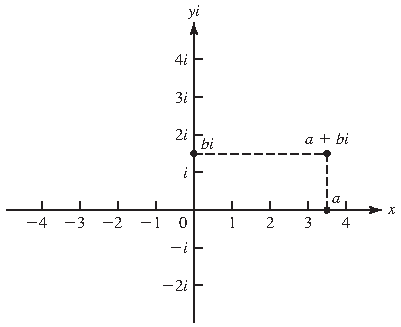
\includegraphics[width=0.550\linewidth,height=.8\textheight,keepaspectratio]{assets/p050_07.pdf}\end{center}
\begin{center}\small\textbf{3.6 Figure}\end{center}
\end{BookFloat}

\BookTextHeading{\textbf{Complex Numbers}  }

\noindent A real number can be visualized geometrically as a point on a line that we often regard as an \BookInline{x-}axis. A complex number can be regarded as a point in the Euclidean plane, as shown in Fig. 3.6. Note that we label the vertical axis as the \BookInline{yi-}axis rather than just the \BookInline{y-}axis, and label the point one unit above the origin with \BookInline{i} rather than 1. The point with Cartesian coordinates \BookInline{(a,\allowbreak b)} is labeled \BookInline{a+ } \textit{bi} in Fig. 3.6. The set \BookInline{\mathbb{C}} of\textbf{ complex numbers} is defined by

\begin{center}\begin{adjustbox}{max width=\linewidth}\BookInline{\displaystyle \mathbb{C}= \{a+ bi\mid a,\allowbreak b\in \mathbb{R}\}.}\end{adjustbox}\end{center}

\noindent We consider \BookInline{\mathbb{R}} to be a subset of the complex numbers by identifying a real number \BookInline{r} with the complex number \BookInline{r+ 0i.} For example, we write \BookInline{3+ 0i} as 3 and \BookInline{- \pi + 0i} as \BookInline{- \pi } and \BookInline{0+ 0i} as 0. Similarly, we write \BookInline{0+ 1i} as \BookInline{i} and \BookInline{0+ si} as \BookInline{si.}

\end{BookBody}

% Source PDF page 51; original printed page 34
\BookSource{51}{34}
\BookNarrativetrue

\begin{BookBody}

Complex numbers were developed after the development of real numbers. The complex number \BookInline{i} was\textit{ invented} to provide a solution to the quadratic equation \BookInline{x^{2}= - 1,\allowbreak } so we require that

\begin{center}\begin{adjustbox}{max width=\linewidth}\BookInline{\displaystyle i^{2}= - 1.(1)}\end{adjustbox}\end{center}

\noindent Unfortunately\BookInline{,\allowbreak i} has been called an\textbf{ imaginary number,} and this terminology has led generations of students to view the complex numbers with more skepticism than the real numbers. Actually,\textit{ all} numbers, such as \BookInline{1,\allowbreak 3,\allowbreak \pi,\allowbreak - \sqrt{3},\allowbreak } and \BookInline{i} are inventions of our minds. There is no physical entity that\textit{ is} the number 1. If there were, it would surely be in a place of honor in some great scientific museum, and past it would file a steady stream of mathematicians, gazing at 1 in wonder and awe. A basic goal of this text is to show how we can invent solutions of polynomial equations when the coefficients of the polynomial may not even be real numbers!

\BookTextHeading{\textbf{Multiplication of Complex Numbers}  }

\noindent The product \BookInline{(a+ } \textit{bi}\BookInline{)(c+ } \textit{di}) is defined in the way it must be if we are to enjoy the familiar properties of real arithmetic and require that \BookInline{i^{2}= - 1,\allowbreak } in accord with Eq. (1). Namely, we see that we want to have

\begin{center}\begin{adjustbox}{max width=\linewidth}\BookInline{\displaystyle \begin{aligned}(a+ bi)(c+ di)&= ac+ adi+ bci+ bdi^{2} \\ &= ac+ adi+ bci+ bd(- 1) \\ &= (ac- bd)+ (ad+ bc)i.\end{aligned}}\end{adjustbox}\end{center}

\noindent Consequently, we define multiplication of \BookInline{z_{1}= a+ } \textit{bi} and \BookInline{z_{2}= c+ } \textit{di} as

\begin{center}\begin{adjustbox}{max width=\linewidth}\BookInline{\displaystyle z_{1}z_{2}= (a+ bi)(c+ di)= (ac- bd)+ (ad+ bc)i,\allowbreak (2)}\end{adjustbox}\end{center}

\noindent which is of the form \BookInline{r+ si} with \BookInline{r= } \textit{ac} \BookInline{- bd} and \BookInline{s= ad+ bc.} It is routine to check that the usual properties \BookInline{z_{1}z_{2}= z_{2}z_{1}(}commutative\BookInline{),\allowbreak z_{1}(z_{2}z_{3})= (z_{1}z_{2})z_{3}(}associative), and \BookInline{z_{1}(z_{2}+ z_{3})= z_{1}z_{2}+ z_{1}z_{3}(}distributive) all hold for all \BookInline{z_{1},\allowbreak z_{2},\allowbreak z_{3}\in \mathbb{C}.}

\BookLabel{3.7 Example} 

\BookTextHeading{Compute (2 \ensuremath{-} 5\textit{i})(8 + 3\textit{i}).  }

\BookLabel{\textit{Solution}} We don’t memorize Eq. (2), but rather we compute the product as we did to motivate that equation. We have

\begin{center}\begin{adjustbox}{max width=\linewidth}\BookInline{\displaystyle (2- 5i)(8+ 3i)= 16+ 6i- 40i+ 15= 31- 34i.\blacktriangle}\end{adjustbox}\end{center}

\noindent To establish the geometric meaning of complex multiplication, we first define the\textbf{ abso}\textbf{lute value} \BookInline{|a+ } \textit{bi}\BookInline{|} of \BookInline{a+ } \textit{bi} by

\begin{center}\begin{adjustbox}{max width=\linewidth}\BookInline{\displaystyle |a+ bi|= \sqrt{a^{2}}+ b^{2}.}\end{adjustbox}\end{center}

\noindent This absolute value is a nonnegative real number and is the distance from \BookInline{a+ } \textit{bi} to the origin in Fig. 3.6. We can now describe a complex number \BookInline{z} in the polar-coordinate form

\begin{center}\begin{adjustbox}{max width=\linewidth}\BookInline{\displaystyle z= |z|(\;\text{cos}\;\theta + i\;\text{sin}\;\theta ),\allowbreak (4)}\end{adjustbox}\end{center}

\noindent where \BookInline{\theta } is the angle measured counterclockwise from the positive \BookInline{x-}axis to the vector from 0 to \BookInline{z,\allowbreak } as shown in Fig. 3.8. A famous formula due to Leonard Euler states that

\begin{center}\begin{adjustbox}{max width=\linewidth}\BookInline{\displaystyle e^{i\theta }= \;\text{cos}\;\theta + i\;\text{sin}\;\theta .}\end{adjustbox}\end{center}

\begin{center}\begin{adjustbox}{max width=\linewidth}\BookInline{\displaystyle \;\text{Euler}\;\text{’}\;\text{s Formula}\;}\end{adjustbox}\end{center}

\end{BookBody}

% Source PDF page 52; original printed page 35
\BookSource{52}{35}
\BookNarrativetrue

\begin{BookBody}

\begin{BookFloat}{03_abelian_examples-p52-0}
\begin{center}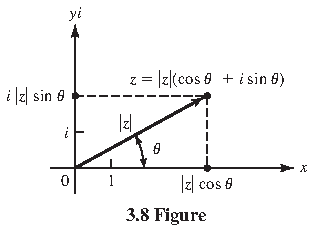
\includegraphics[width=0.427\linewidth,height=.8\textheight,keepaspectratio]{assets/p052_01.pdf}\end{center}
\end{BookFloat}

\noindent We ask you to derive Euler’s formula formally from the power series expansions for \BookInline{e^{\theta },\allowbreak } cos \BookInline{\theta,\allowbreak } and sin \BookInline{\theta } in Exercise 43. Using this formula, we can express \BookInline{z} in Eq. (4) as \BookInline{z= |z|e^{i\theta }.} Let us set

\begin{center}\begin{adjustbox}{max width=\linewidth}\BookInline{\displaystyle z_{1}= |z_{1}|e^{i\theta _{1}}\;\text{and}\;z_{2}= |z_{2}|e^{i\theta _{2}}}\end{adjustbox}\end{center}

\noindent and compute their product in this form, assuming that the usual laws of exponentiation hold with complex number exponents. We obtain

\begin{center}\begin{adjustbox}{max width=\linewidth}\BookInline{\displaystyle \begin{aligned}z_{1}z_{2}&= |z_{1}|e^{i\theta _{1}}|z_{2}|e^{i\theta _{2}}= |z_{1}||z_{2}|e^{i(\theta _{1}+ \theta _{2})} \\ &= |z_{1}||z_{2}|[\;\text{cos}\;(\theta _{1}+ \theta _{2})+ i\;\text{sin}\;(\theta _{1}+ \theta _{2})].(5)\end{aligned}}\end{adjustbox}\end{center}

\noindent Note that Eq. 5 concludes in the polar form of Eq. 4 where \BookInline{|z_{1}z_{2}|= |z_{1}||z_{2}|} and the polar angle \BookInline{\theta } for \BookInline{z_{1}z_{2}} is the sum \BookInline{\theta = \theta _{1}+ \theta _{2}.} Thus, geometrically, we multiply complex numbers by multiplying their absolute values and adding their polar angles, as shown in Fig. 3.9. Exercise 41 indicates how this can be derived via trigonometric identities without recourse to Euler’s formula and assumptions about complex exponentiation.

\begin{BookFloat}{03_abelian_examples-p52-6}
\begin{center}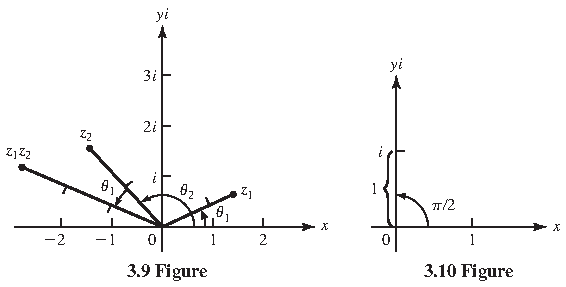
\includegraphics[width=0.777\linewidth,height=.8\textheight,keepaspectratio]{assets/p052_00.pdf}\end{center}
\end{BookFloat}

Note that \BookInline{i} has polar angle \BookInline{\pi /2} and absolute value 1, as shown in Fig. 3.10. Thus \BookInline{i^{2}} has polar angle \BookInline{2(\pi /2)= \pi } and \BookInline{|1\cdot 1|= 1,\allowbreak } so that \BookInline{i^{2}= - 1.}

\BookLabel{3.11 Example} Find all solutions in \BookInline{\mathbb{C}} of the equation \BookInline{z^{2}= i.}

\BookLabel{\textit{Solution}} Writing the equation \BookInline{z^{2}= i} in polar form and using Eq. (5), we obtain

\begin{center}\begin{adjustbox}{max width=\linewidth}\BookInline{\displaystyle |z|^{2}(\;\text{cos}\;2\theta + i\;\text{sin}\;2\theta )= 1(0+ i).}\end{adjustbox}\end{center}

\noindent Thus \BookInline{|z|^{2}= 1,\allowbreak } so \BookInline{|z|= 1.} The angle \BookInline{\theta } for \BookInline{z} must satisfy cos \BookInline{2\theta = 0} and sin \BookInline{2\theta = 1.} Consequently\BookInline{,\allowbreak 2\theta = (\pi /2)+ n(2\pi ),\allowbreak } so \BookInline{\theta = (\pi /4)+ n\pi } for an integer \BookInline{n.} The values of

\end{BookBody}

% Source PDF page 53; original printed page 36
\BookSource{53}{36}
\BookNarrativetrue

\begin{BookBody}

\noindent \BookInline{n} yielding values \BookInline{\theta } where \BookInline{0\leq \theta <2\pi } are 0 and 1, yielding \BookInline{\theta = \pi /4} or \BookInline{\theta = 5\pi /4.} Our solutions are

\begin{center}\begin{adjustbox}{max width=\linewidth}\BookInline{\displaystyle z _ { 1 } = 1 \Bigg ( \cos \frac { \pi } { 4 } + i \sin \frac { \pi } { 4 } \Bigg ) \qquad \mathrm { a n d } \qquad z _ { 2 } = 1 \Bigg ( \cos \frac { 5 \pi } { 4 } + i \sin \frac { 5 \pi } { 4 } \Bigg )}\end{adjustbox}\end{center}

\noindent or

\begin{center}\begin{adjustbox}{max width=\linewidth}\BookInline{\displaystyle z _ { 1 } = \frac { 1 } { \sqrt { 2 } } ( 1 + i ) \qquad \mathrm { a n d } \qquad z _ { 2 } = \frac { - 1 } { \sqrt { 2 } } ( 1 + i ) .}\end{adjustbox}\end{center} \BookEnd{\blacktriangle}

\BookLabel{3.12 Example} Find all solutions of \BookInline{z^{4}= - 16.}

\BookLabel{\textit{Solution}} As in Example 3.11 we write the equation in polar form, obtaining

\begin{center}\begin{adjustbox}{max width=\linewidth}\BookInline{\displaystyle |z|^{4}(\;\text{cos}\;4\theta + i\;\text{sin}\;4\theta )= 16(- 1+ 0i).}\end{adjustbox}\end{center}

\noindent Consequently\BookInline{,\allowbreak |z|^{4}= 16,\allowbreak } so \BookInline{|z|= 2} while cos \BookInline{4\theta = - 1} and sin \BookInline{4\theta = 0.} We find that \BookInline{4\theta = \pi + n(2\pi ),\allowbreak } so \BookInline{\theta = (\pi /4)+ n(\pi /2)} for integers \BookInline{n.} The different values of \BookInline{\theta } obtained where \BookInline{0\leq \theta <2\pi } are \BookInline{\pi /4,\allowbreak 3\pi /4,\allowbreak 5\pi /4,\allowbreak } and \BookInline{7\pi /4.} Thus one solution of \BookInline{z^{4}= - 16} is

\begin{center}\begin{adjustbox}{max width=\linewidth}\BookInline{\displaystyle 2\bigg(\cos\frac{\pi}{4}+i\sin\frac{\pi}{4}\bigg)=2\bigg(\frac{1}{\sqrt{2}}+\frac{1}{\sqrt{2}}i\bigg)=\sqrt{2}(1+i).}\end{adjustbox}\end{center}

\noindent In a similar way, we find three more solutions,

\begin{center}\begin{adjustbox}{max width=\linewidth}\BookInline{\displaystyle \sqrt{2}(- 1+ i),\allowbreak \sqrt{2}(- 1- i),\allowbreak \;\text{and}\;\sqrt{2}(1- i).}\end{adjustbox}\end{center} \BookEnd{\blacktriangle}

The last two examples illustrate that we can find solutions of an equation \BookInline{z^{n}= } \BookInline{a+ } \textit{bi} by writing the equation in polar form. There will always be \BookInline{n} solutions, provided that \BookInline{a+ } \textit{bi}\BookInline{\neq 0.} Exercises 16 through 21 ask you to solve equations of this type.

We will not use addition or division of complex numbers, but we probably should mention that addition is given by

\begin{center}\begin{adjustbox}{max width=\linewidth}\BookInline{\displaystyle (a+ bi)+ (c+ di)= (a+ c)+ (b+ d)i.(6)}\end{adjustbox}\end{center}

\noindent and division of \BookInline{a+ } \textit{bi} by nonzero \BookInline{c+ } \textit{di} can be performed using only division of real numbers as follows:

\begin{center}\begin{adjustbox}{max width=\linewidth}\BookInline{\displaystyle \begin{aligned}\frac{a + bi}{c + di} &= \frac{a + bi}{c + di} \cdot \frac{c - di}{c - di} = \frac{(ac + bd) + (bc - ad)i}{c^2 + d^2} \\&= \frac{ac + bd}{c^2 + d^2} + \frac{bc - ad}{c^2 + d^2}i.\end{aligned}}\end{adjustbox}\end{center}

\begin{BookFloat}{03_abelian_examples-p53-18}
\begin{center}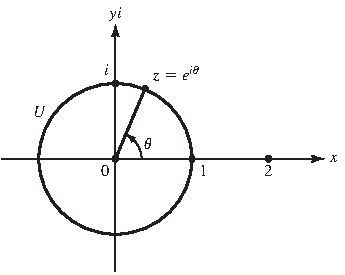
\includegraphics[width=0.473\linewidth,height=.8\textheight,keepaspectratio]{assets/p053_19.pdf}\end{center}
\begin{center}\small\textbf{3.13 Figure}\end{center}
\end{BookFloat}

\end{BookBody}

% Source PDF page 54; original printed page 37
\BookSource{54}{37}
\BookNarrativetrue

\begin{BookBody}

\BookTextHeading{\textbf{Algebra on the Unit Circle}  }

\noindent Let \BookInline{U= \{z\in \mathbb{C}\mid |z|= 1\},\allowbreak } so that \BookInline{U} is the circle in the Euclidean plane with center at the origin and radius 1, as shown in Fig. 3.13.

\BookLabel{3.14 Theorem} \BookInline{\langle U,\allowbreak \cdot \rangle } is an abelian group.

\BookLabel{\textit{Proof}} We first check that \BookInline{U} is closed under multiplication. Let \BookInline{z_{1},\allowbreak z_{2}\in U.} Then \BookInline{|z_{1}|= |z_{2}|= 1,\allowbreak } which implies that \BookInline{|z_{1}z_{1}|= 1,\allowbreak } showing \BookInline{z_{1}z_{2}\in U.}

Since multiplication of complex numbers is associative and commutative in general, multiplication in \BookInline{U} is also associative and commutative, which verifies \BookInline{\mathcal{G}_{1}} and the condition for abelian.

The number \BookInline{1\in U} is the identity, verifying condition \BookInline{\mathcal{G}_{2}.}

For each \BookInline{a+ } \textit{bi} \BookInline{\in U,\allowbreak }

\begin{center}\begin{adjustbox}{max width=\linewidth}\BookInline{\displaystyle (a+ bi)(a- bi)= a^{2}- (bi)^{2}= a^{2}+ b^{2}= |a+ bi|^{2}= 1.}\end{adjustbox}\end{center}

\noindent So the inverse of \BookInline{a+ } \textit{bi} is \BookInline{a- } \textit{bi}, which verifies condition \BookInline{\mathcal{G}_{3}.} Thus \BookInline{U} is an abelian group under multiplication\BookInline{.}\BookEnd{\blacklozenge}

Figure 3.13 gives us a way of relabeling points in \BookInline{U} as points in \BookInline{\mathbb{R}_{2\pi }.} We simply relabel \BookInline{z} as \BookInline{\theta } where \BookInline{0\leq \theta <2\pi.} Let \BookInline{f:U\to \mathbb{R}_{2\pi }} be given by \BookInline{f(z)= \theta } according to this relabeling. Then for \BookInline{z_{1},\allowbreak z_{2}\in U,\allowbreak f(z_{1}z_{2})= f(z_{1})+ _{2\pi }f(z_{2})} since multiplying in \BookInline{U} simply adds the corresponding angles:

\begin{center}\begin{adjustbox}{max width=\linewidth}\BookInline{\displaystyle \;\text{if}\;z_{1}\leftrightarrow \theta _{1}\;\text{and}\;z_{2}\leftrightarrow \theta _{2},\allowbreak \;\text{then}\;z_{1}\cdot z_{2}\leftrightarrow (\theta _{1}+ _{2\pi }\theta _{2}).(8)}\end{adjustbox}\end{center}

\noindent Recall that all that remains to show that \BookInline{\mathbb{R}_{2\pi }} is a group is to show that \BookInline{+ _{2\pi }} is associative. Since the operations of multiplication in \BookInline{U} and addition modulo \BookInline{2\pi } in \BookInline{\mathbb{R}_{2\pi }} are the same using the above relabeling and multiplication in \BookInline{U} is associative, addition modulo \BookInline{2\pi } is also associative. This completes the proof that \BookInline{\langle \mathbb{R}_{2\pi },\allowbreak + _{2\pi }\rangle } is a group. Furthermore, the relabeling (8) shows that the two groups \BookInline{\langle U,\allowbreak \cdot \rangle } and \BookInline{\langle \mathbb{R}_{2\pi },\allowbreak + _{2\pi }\rangle } are isomorphic. In Exercise 45, you will be asked to prove that for any \BookInline{b>0} and \BookInline{c>0,\allowbreak \langle \mathbb{R}_{b},\allowbreak + _{b}\rangle } is an abelian group and \BookInline{\langle \mathbb{R}_{b},\allowbreak + _{b}\rangle \simeq \langle \mathbb{R}_{c},\allowbreak + _{c}\rangle.} Since \BookInline{\langle \mathbb{R}_{2\pi },\allowbreak + _{2\pi }\rangle } is isomorphic with \BookInline{\langle U,\allowbreak \cdot \rangle,\allowbreak } for every \BookInline{c>0,\allowbreak \langle \mathbb{R}_{c},\allowbreak + _{c}\rangle } is also isomorphic with \BookInline{\langle U,\allowbreak \cdot \rangle,\allowbreak } meaning they have the same algebraic properties.

\BookLabel{3.15 Example} The equation \BookInline{z\cdot z\cdot z\cdot z= 1} in \BookInline{U} has exactly four solutions, namely\BookInline{,\allowbreak 1,\allowbreak i,\allowbreak - 1,\allowbreak } and \BookInline{- i.} Now \BookInline{1\in U} and \BookInline{0\in \mathbb{R}_{2\pi }} correspond, and the equation \BookInline{x+ _{2\pi }x+ _{2\pi }x+ _{2\pi }x= 0} in \BookInline{\mathbb{R}_{2\pi }} has exactly four solutions, namely\BookInline{,\allowbreak 0,\allowbreak \pi /2,\allowbreak \pi,\allowbreak } and \BookInline{3\pi /2,\allowbreak } which, of course, correspond to \BookInline{1,\allowbreak i,\allowbreak - 1,\allowbreak } and \BookInline{- i,\allowbreak } respectively\BookInline{.}\BookEnd{\blacktriangle}

\BookTextHeading{\textbf{Roots of Unity}  }

\noindent The elements of the set \BookInline{U_{n}= \{z\in \mathbb{C}\mid z^{n}= 1\}} are called the \BookInline{n}th\textbf{ roots of unity}. In Exercise 46 you are asked to prove that \BookInline{U_{n}} is a group under multiplication. Using the techniques from Examples 3.11 and 3.12, we see that the elements of this set are the numbers \BookInline{2\pi 2\pi }

\begin{center}\begin{adjustbox}{max width=\linewidth}\BookInline{\displaystyle e ^ { \left( m { \frac { 2 \pi } { n } } \right) i } = \cos \left( m { \frac { 2 \pi } { n } } \right) + i \sin \left( m { \frac { 2 \pi } { n } } \right) \quad { \mathrm { f o r } } \; m = 0 ,\allowbreak  1 ,\allowbreak  2 ,\allowbreak  \ldots ,\allowbreak  n - 1 .}\end{adjustbox}\end{center}

\noindent They all have absolute value 1, so \BookInline{U_{n}\subset U.} If we let \BookInline{\zeta = } cos \BookInline{2n\pi + i} sin \BookInline{2n\pi,\allowbreak } then these \BookInline{n}th roots of unity can be written as

\begin{center}\begin{adjustbox}{max width=\linewidth}\BookInline{\displaystyle 1= \zeta ^{0},\allowbreak \zeta ^{1},\allowbreak \zeta ^{2},\allowbreak \zeta ^{3},\allowbreak \cdots ,\allowbreak \zeta ^{n- 1}.(9)}\end{adjustbox}\end{center}

\noindent Because \BookInline{\zeta ^{n}= 1,\allowbreak } these \BookInline{n} powers of \BookInline{\zeta } are closed under multiplication. For example, with \BookInline{n= 10,\allowbreak } we have 6 8 14 10 4 4 4 \BookInline{\zeta \zeta = \zeta = \zeta \zeta = 1\cdot \zeta = \zeta.}

\end{BookBody}

% Source PDF page 55; original printed page 38
\BookSource{55}{38}
\BookNarrativetrue

\begin{BookBody}

\noindent Thus we see that we can compute \BookInline{\zeta ^{i}\zeta ^{j}} by computing \BookInline{i+ _{n}j,\allowbreak } viewing \BookInline{i} and \BookInline{j} as elements of \BookInline{\mathbb{Z}_{n}.}

By relabeling an element \BookInline{\zeta ^{m}\in U_{n}} to \BookInline{m\in \mathbb{Z}_{n}} we can see that addition modulo \BookInline{n} in \BookInline{\mathbb{Z}_{n}} is also associative, which completes the proof that \BookInline{\langle \mathbb{Z}_{n},\allowbreak + _{n}\rangle } is an abelian group.

\BookLabel{3.16 Example} We solve the equation \BookInline{x+ _{8}x+ _{8}x= 1} in \BookInline{\mathbb{Z}_{8}} using trial and error. We note that neither 0, 1, nor 2 is a solution simply by substitution. However, substituting \BookInline{x= 3} gives \BookInline{3+ _{8}3+ _{8}3= 6+ _{8}3= 1,\allowbreak } which shows \BookInline{x= 3} is a solution. We can also check by substituting that neither 4, 5, 6, nor 7 are solutions. So the only solution is \BookInline{x= 3.} Because \BookInline{\mathbb{Z}_{8}} is isomorphic with \BookInline{U_{8}} by the correspondence \BookInline{k\in \mathbb{Z}_{8}} corresponds with \BookInline{\zeta ^{k},\allowbreak } the corresponding equation in \BookInline{U_{8}} is \BookInline{z \cdot z \cdot z = \zeta = e ^ { \frac { 2 \pi } { 8 } i }}. Without further calculations we know that there is only one solution to \BookInline{z\cdot z\cdot z= \zeta } in \BookInline{U_{8}} and that solution is \BookInline{z = \zeta^{3} = e^{3\frac{2\pi}{8}i} = \cos(6\pi/8) + i\sin(6\pi/8) = -\frac{\sqrt{2}}{2} + \frac{\sqrt{2}}{2}i} since this is the corresponding solution in \BookInline{\mathbb{Z}_{8}.}

There are three solutions to \BookInline{z^{3}= \zeta } in \BookInline{U.} We leave it to the reader to find the solutions and check that only one of them\BookInline{,\allowbreak \zeta ^{3},\allowbreak } is in \BookInline{U_{8}.}\BookEnd{\blacktriangle}

\noindent We summarize the results of this section.

\BookExercise{1.}{For any \BookInline{n\in \mathbb{Z}^{+ },\allowbreak \mathbb{Z}_{n}} is an abelian group under addition modulo \BookInline{n.}}

\BookExercise{2.}{For any \BookInline{n\in \mathbb{Z}^{+ },\allowbreak \mathbb{Z}_{n}} is isomorphic with \BookInline{U_{n},\allowbreak } an abelian group under complex number multiplication.}

\BookExercise{3.}{For any \BookInline{c>0,\allowbreak R_{c}} under addition modulo \BookInline{c} is a group.}

\BookExercise{4.}{\BookInline{U} under multiplication is a group.}

\BookExercise{5.}{For any \BookInline{c\in \mathbb{R}^{+ },\allowbreak \mathbb{R}_{c}} under addition modulo \BookInline{c} is isomorphic with \BookInline{U} under multiplication.}

\end{BookBody}

\BookNarrativefalse

\begin{BookBody}

\BookExerciseTitle{3} \BookEnd{\blacksquare}

\noindent In Exercises 1 through 9 compute the given arithmetic expression and give the answer in the form \BookInline{a+ } \textit{bi} for \BookInline{a,\allowbreak b\in \mathbb{R}.}

\BookExercise{1.}{\BookInline{i^{3}}}

\BookExercise{2.}{\BookInline{i^{4}}}

\BookExercise{3.}{26 \BookInline{i}}

\BookExercise{4.}{\BookInline{(- i)^{39}}}

\BookExercise{5.}{\BookInline{(3- 2i)(6+ i)}}

\BookExercise{6.}{\BookInline{(8+ 2i)(3- i)}}

\BookExercise{7.}{\BookInline{(2- 3i)(4+ i)+ (6- 5i)}}

\BookExercise{8.}{\BookInline{(1+ i)^{3}}}

\BookExercise{9.}{\BookInline{(1- i)^{5}(}Use the binomial theorem.)}

\BookExercise{10.}{Find \BookInline{|5- 12i|.}}

\BookExercise{11.}{Find \BookInline{|\pi + ei|.}}

\noindent In Exercises 12 through 15 write the given complex number \BookInline{z} in the polar form \BookInline{|z|(p+ qi)} where \BookInline{|p+ qi|= 1.}

\BookExercise{12.}{\BookInline{3- 4i}}

\BookExercise{13.}{\BookInline{- 1- i}}

\BookExercise{14.}{\BookInline{12+ 5i}}

\BookExercise{15.}{\BookInline{- 3+ 5i}}

\noindent In Exercises 16 through 21, find all solutions in \BookInline{\mathbb{C}} of the given equation.

\BookExercise{16.}{\BookInline{z^{4}= 1}}

\BookExercise{17.}{\BookInline{z^{4}= - 1}}

\BookExercise{18.}{\BookInline{z^{3}= - 125}}

\BookExercise{19.}{\BookInline{z^{3}= - 27i}}

\BookExercise{20.}{\BookInline{z^{6}= 1}}

\BookExercise{21.}{\BookInline{z^{6}= - 64}}

\noindent In Exercises 22 through 27, compute the given expression using the indicated modular addition.

\BookExercise{22.}{\BookInline{10+ _{17}16}}

\BookExercise{23.}{\BookInline{14+ _{99}92}}

\BookExercise{24.}{\BookInline{3.141+ _{4}2.718}}

\BookExercise{25.}{\BookInline{{ \textstyle { \frac { 1 } { 2 } } } + _ { 1 } { \textstyle { \frac { 7 } { 8 } } }}}

\BookExercise{26.}{\BookInline{\frac { 3 \pi } { 4 } + _ { 2 \pi } \frac { 3 \pi } { 2 }}}

\BookExercise{27.}{\BookInline{2\sqrt{2}+_{\sqrt{32}}3\sqrt{2}}}

\BookExercise{28.}{Explain why the expression \BookInline{5+ _{6}8} in \BookInline{\mathbb{R}_{6}} makes no sense.}

\end{BookBody}

% Continuation on source PDF page 56, preceding Section 4
\BookNarrativefalse

\begin{BookBody}

\noindent In Exercises 29 through 34, find\textit{ all} solutions \BookInline{x} of the given equation.

\BookExercise{29.}{\BookInline{x+ _{10}7= 3} in \BookInline{\mathbb{Z}_{10}}}

\BookExercise{30.}{\BookInline{x+ _{2\pi }\pi = \frac{\pi }{2}} in \BookInline{\mathbb{R}_{2\pi }}}

\BookExercise{31.}{\BookInline{x+ _{7}x= 3} in \BookInline{\mathbb{Z}_{7}}}

\BookExercise{32.}{\BookInline{x+ _{13}x+ _{13}x= 5} in \BookInline{\mathbb{Z}_{13}}}

\BookExercise{33.}{\BookInline{x+ _{12}x= 2} in \BookInline{\mathbb{Z}_{12}}}

\BookExercise{34.}{\BookInline{x+ _{8}x+ _{8}x+ _{8}x= 4} in \BookInline{\mathbb{Z}_{8}}}

\BookExercise{35.}{Prove or give a counterexample to the statement that for any \BookInline{n\in \mathbb{Z}^{+ }} and \BookInline{a\in \mathbb{Z}_{n},\allowbreak } the equation \BookInline{x+ _{n}x= a} has at most two solutions in \BookInline{\mathbb{Z}_{n}.}}

\BookExercise{36.}{Prove or give a counterexample to the statement that for any \BookInline{n\in \mathbb{Z}^{+ }} and \BookInline{a\in \mathbb{Z}_{n},\allowbreak } if \BookInline{n} is not a multiple of 3, then the equation \BookInline{x+ _{n}x+ _{n}x= a} has exactly one solution in \BookInline{\mathbb{Z}_{n}.}}

\BookExercise{37.}{There is an isomorphism of \BookInline{U_{8}} with \BookInline{\mathbb{Z}_{8}} in which \BookInline{\zeta = e^{i(\pi /4)}\leftrightarrow 5} and \BookInline{\zeta ^{2}\leftrightarrow 2.} Find the element of \BookInline{\mathbb{Z}_{8}} that corresponds to each of the remaining six elements \BookInline{\zeta ^{m}} in \BookInline{U_{8}} for \BookInline{m= 0,\allowbreak 3,\allowbreak 4,\allowbreak 5,\allowbreak 6,\allowbreak } and 7.}

\BookExercise{38.}{There is an isomorphism of \BookInline{U_{7}} with \BookInline{\mathbb{Z}_{7}} in which \BookInline{\zeta = e^{i(2\pi /7)}\leftrightarrow 4.} Find the element in \BookInline{\mathbb{Z}_{7}} to which \BookInline{\zeta ^{m}} must correspond for \BookInline{m= 0,\allowbreak 2,\allowbreak 3,\allowbreak 4,\allowbreak 5,\allowbreak } and 6.}

\BookExercise{39.}{Why can there be no isomorphism of \BookInline{U_{6}} with \BookInline{\mathbb{Z}_{6}} in which \BookInline{\zeta = e^{i(\pi /3)}} corresponds to 4?}

\BookExercise{40.}{Derive the formulas}

\begin{center}\begin{adjustbox}{max width=\linewidth}\BookInline{\displaystyle \;\text{sin}\;(a+ b)= \;\text{sin}\;a\;\text{cos}\;b+ \;\text{cos}\;a\;\text{sin}\;b}\end{adjustbox}\end{center}

and

\begin{center}\begin{adjustbox}{max width=\linewidth}\BookInline{\displaystyle \;\text{cos}\;(a+ b)= \;\text{cos}\;a\;\text{cos}\;b- \;\text{sin}\;a\;\text{sin}\;b}\end{adjustbox}\end{center}

by using Euler’s formula and computing \BookInline{e^{ia}e^{ib}.}

\BookExercise{41.}{Let \BookInline{z_{1}= |z_{1}|(}cos \BookInline{\theta _{1}+ i} sin \BookInline{\theta _{1})} and \BookInline{z_{2}= |z_{2}|(}cos \BookInline{\theta _{2}+ i} sin \BookInline{\theta _{2}).} Use the trigonometric identities in Exercise 40 to derive \BookInline{z_{1}z_{2}= |z_{1}||z_{2}|[}cos\BookInline{(\theta _{1}+ \theta _{2})+ i} sin\BookInline{(\theta _{1}+ \theta _{2})].}}

\BookExercise{42.}{\textbf{. a} Derive a formula for cos \BookInline{3\theta } in terms of sin \BookInline{\theta } and cos \BookInline{\theta } using Euler’s formula.}

\BookExercise{b.}{Derive the formula cos \BookInline{3\theta = 4} cos\BookInline{3\theta - 3} cos \BookInline{\theta } from part (a) and the identity sin\BookInline{2\theta + } cos\BookInline{2\theta = 1.(}We will have use for this identity in Section 41.)}

\BookExercise{43.}{Recall the power series expansions}

\begin{center}\begin{adjustbox}{max width=\linewidth}\BookInline{\displaystyle e ^ { x } = 1 + x + { \frac { x ^ { 2 } } { 2 ! } } + { \frac { x ^ { 3 } } { 3 ! } } + { \frac { x ^ { 4 } } { 4 ! } } + \cdots + { \frac { x ^ { n } } { n ! } } + \cdots ,\allowbreak }\end{adjustbox}\end{center}

\begin{center}\begin{adjustbox}{max width=\linewidth}\BookInline{\displaystyle \sin x = x - { \frac { x ^ { 3 } } { 3 ! } } + { \frac { x ^ { 5 } } { 5 ! } } - { \frac { x ^ { 7 } } { 7 ! } } + \cdots + ( - 1 ) ^ { n - 1 } { \frac { x ^ { 2 n - 1 } } { ( 2 n - 1 ) ! } } + \cdots   ,\allowbreak    { \mathrm { a n d } }}\end{adjustbox}\end{center}

\begin{center}\begin{adjustbox}{max width=\linewidth}\BookInline{\displaystyle \cos x = 1 - \frac{x^2}{2!} + \frac{x^4}{4!} - \frac{x^6}{6!} + \cdots + (-1)^n \frac{x^{2n}}{(2n)!} + \cdots}\end{adjustbox}\end{center}

from calculus. Derive Euler’s formula \BookInline{e^{i\theta }= } cos \BookInline{\theta + i} sin \BookInline{\theta } formally from these three series expansions.

\BookExercise{44.}{Prove that for any \BookInline{n\in \mathbb{Z}^{+ },\allowbreak \langle \mathbb{Z}_{n},\allowbreak + _{n}\rangle } is associative without using the fact that \BookInline{U_{n}} is associative.}

\BookExercise{45.}{Let \BookInline{b,\allowbreak c\in \mathbb{R}^{+ }.} Find a one-to-one and onto function \BookInline{f:\mathbb{R}_{b}\to \mathbb{R}_{c}} that has the homomorphism property. Conclude that \BookInline{\mathbb{R}_{c}} is an abelian group that is isomorphic with \BookInline{U.}}

\BookExercise{46.}{Prove that for any \BookInline{n\geq 1,\allowbreak U_{n}} is a group.}

\end{BookBody}
\ifdefined\BookMaster\let\BookFinish\relax\else\def\BookFinish{\end{document}}\fi\BookFinish

\clearpage
% !TeX program = xelatex
\ifdefined\BookMaster\else
\documentclass[11pt,oneside]{article}
% !TeX program = xelatex
\usepackage[b5paper,left=22mm,right=22mm,top=20mm,bottom=22mm,footskip=11mm]{geometry}
\usepackage{fontspec}
\setmainfont{TeX Gyre Termes}
\setsansfont{TeX Gyre Heros}
\usepackage{amsmath,amssymb,mathtools,amsthm}
\renewcommand{\cdots}{\mathinner{\cdotp\cdotp\cdotp}}
\usepackage{graphicx,adjustbox,array,booktabs,longtable,multirow,enumitem,changepage,needspace}
\usepackage[table]{xcolor}
\usepackage{fancyhdr}
\raggedbottom
\interfootnotelinepenalty=10000
\newcommand{\BookFootnote}[2]{\begingroup\renewcommand{\thefootnote}{\fnsymbol{footnote}}\footnote[#1]{#2}\endgroup}
\newcommand{\BookFootnoteMark}[1]{\begingroup\renewcommand{\thefootnote}{\fnsymbol{footnote}}\footnotemark[#1]\endgroup}
\newcommand{\BookFootnoteText}[2]{\begingroup\renewcommand{\thefootnote}{\fnsymbol{footnote}}\footnotetext[#1]{#2}\endgroup}
\newenvironment{BookFloat}[1]{\par\addvspace{.6\baselineskip}\noindent\def\BookFloatID{#1}\begin{minipage}{\linewidth}\phantomsection\label{bookfloat:#1:start}}{\phantomsection\label{bookfloat:\BookFloatID:end}\end{minipage}\par\addvspace{.6\baselineskip}}

\usepackage[unicode,hidelinks]{hyperref}
\pagestyle{fancy}
\fancyhf{}
\newcommand{\BookFooter}{}
\fancyfoot[L]{\parbox[b]{\dimexpr\textwidth-15mm}{\footnotesize\BookFooter}}
\fancyfoot[R]{\footnotesize\thepage}
\renewcommand{\headrulewidth}{0pt}
\renewcommand{\footrulewidth}{0pt}
\setlength{\parindent}{0pt}
\setlength{\parskip}{0.2em}
\setlength{\emergencystretch}{3em}
\setlist{nosep,leftmargin=1.7em,labelsep=.65em}
\newif\ifBookNarrative
\BookNarrativetrue
\newenvironment{BookBody}{\setlength{\parindent}{0pt}}{}
\newcommand{\BookStatement}[1]{\par\addvspace{.6\baselineskip}\noindent #1\enspace\ignorespaces}
\newcommand{\BookLabel}[1]{\par\addvspace{.6\baselineskip}\needspace{3\baselineskip}\noindent\textbf{#1}\quad\ignorespaces}
\newcommand{\BookHeading}[1]{\par\addvspace{\baselineskip}\needspace{4\baselineskip}\noindent{\large\bfseries #1}\par\medskip}
\newcommand{\BookSubheading}[1]{\par\addvspace{.7\baselineskip}\needspace{3\baselineskip}\noindent{\bfseries #1}\par\smallskip}
\newcommand{\BookTextHeading}[1]{\par\addvspace{.7\baselineskip}\needspace{3\baselineskip}\noindent #1\par\smallskip}
\newcommand{\BookSectionTitle}[2]{\par\addvspace{1.2\baselineskip}\needspace{5\baselineskip}\noindent\colorbox{gray!25}{\sffamily\bfseries\small SECTION #1}\quad{\large\bfseries #2}\par\medskip}
\newcommand{\BookExerciseTitle}[1]{\par\addvspace{\baselineskip}\needspace{4\baselineskip}\noindent{\color{gray}\rule{1.5mm}{1.5mm}}\enspace{\large\bfseries Exercises #1}\par\medskip}
\newcommand{\BookBullet}[1]{\begin{list}{\textbullet}{\setlength{\leftmargin}{1.7em}\setlength{\labelwidth}{1em}\setlength{\labelsep}{.7em}\setlength{\topsep}{0pt}\setlength{\parsep}{0pt}\setlength{\itemsep}{0pt}}\item #1\end{list}}
\newcommand{\BookExercise}[2]{\begin{list}{\textbf{#1}}{\setlength{\leftmargin}{2.2em}\setlength{\labelwidth}{1.5em}\setlength{\labelsep}{.7em}\setlength{\topsep}{.15em}\setlength{\parsep}{0pt}\setlength{\itemsep}{0pt}}\item #2\end{list}}
\newcommand{\BookEnd}[1]{\unskip\nobreak\hfill\ensuremath{#1}}
\newcommand{\BookSource}[2]{\phantomsection\label{sourcepage:#1}} % Source-page anchors, retained through reflow.
\usepackage{multicol}
\usepackage{tikz}
\newcommand{\BookPartEntry}[2]{\par\noindent\makebox[17mm][l]{\bfseries Section #1}#2\par}
\newcommand{\BookPartTitle}[3]{\par\bigskip\noindent\begin{tikzpicture}\node[anchor=north west,inner sep=0pt,outer sep=0pt] (bookpart) at (0,0) {\begin{minipage}{\dimexpr\linewidth-.5pt}\hspace*{26mm}\begin{minipage}[t]{\dimexpr\linewidth-26mm}\begin{adjustbox}{max width=\linewidth}{\fontsize{20}{24}\selectfont\bfseries #2}\end{adjustbox}\par\vspace{6mm}\hrule\vspace{6mm}{\sffamily\footnotesize\setlength{\parskip}{.3em}#3}\vspace{3mm}\end{minipage}\end{minipage}};\path[shade,top color=gray!60,bottom color=white] (0,0) rectangle ([xshift=24mm]bookpart.south west);\node[anchor=north,font=\sffamily\bfseries\small] at (12mm,-2mm) {PART};\node[anchor=north,font=\sffamily\bfseries\Huge] at (12mm,-7mm) {#1};\end{tikzpicture}\par\bigskip}
\newsavebox{\BookMathBox}
\makeatletter
\newcommand{\BookInline}[1]{\leavevmode\hskip0pt\relax\begingroup\in@{\begin}{#1}\ifin@\sbox{\BookMathBox}{\(#1\)}\ifdim\wd\BookMathBox>\dimexpr\linewidth-1em\relax\resizebox{\dimexpr\linewidth-1em\relax}{!}{\usebox{\BookMathBox}}\else\(#1\)\fi\else\in@{\left}{#1}\ifin@\sbox{\BookMathBox}{\(#1\)}\ifdim\wd\BookMathBox>\dimexpr\linewidth-1em\relax\resizebox{\dimexpr\linewidth-1em\relax}{!}{\usebox{\BookMathBox}}\else\(#1\)\fi\else\(#1\)\fi\fi\endgroup\hskip0pt\relax}
\makeatother
\DeclareMathOperator{\Aut}{Aut}
\DeclareMathOperator{\End}{End}
\DeclareMathOperator{\Hom}{Hom}
\DeclareMathOperator{\GF}{GF}
\DeclareMathOperator{\irr}{irr}
\DeclareMathOperator{\lt}{lt}
\DeclareMathOperator{\lp}{lp}
\providecommand{\textcircled}[1]{\textnormal{(#1)}}

\begin{document}
\fi
\renewcommand{\BookFooter}{Section 4 Nonabelian Examples}
\pdfbookmark[0]{Section 4 Nonabelian Examples}{04_nonabelian_examples}
\ifdefined\BookMaster\else\setcounter{page}{39}\fi
% Source PDF page 56; original printed page 39
\BookSource{56}{39}
\BookNarrativetrue

\begin{BookBody}

\BookSectionTitle{4}{Nonabelian Examples}

\BookTextHeading{\textbf{Notation and Terminology}  }

\noindent It is time to explain some conventional notation and terminology used in group theory. Algebraists as a rule do not use a special symbol \BookInline{\ast } to denote a binary operation different from the usual addition and multiplication. They stick with the conventional additive or multiplicative notation and even call the operation\textit{ addition} or\textit{ multiplication,} depending 
% Source PDF page 57; original printed page 40
\BookSource{57}{40}
on the symbol used. The symbol for addition is, of course\BookInline{,\allowbreak +,\allowbreak } and usually multiplication is denoted by juxtaposition without a dot, if no confusion results. Thus in place of the notation \BookInline{a\ast b,\allowbreak } we shall be using either \BookInline{a+ b} to be read “the\textit{ sum} of \BookInline{a} and \BookInline{b,\allowbreak }” or \BookInline{ab} to be read “the\textit{ product} of \BookInline{a} and \BookInline{b.}” There is a sort of unwritten agreement that the symbol \BookInline{+ } should be used only to designate commutative operations. Algebraists feel very uncomfortable when they see \BookInline{a+ b\neq b+ a.} For this reason, when developing our theory in a general situation where the operation may or may not be commutative, we shall always use multiplicative notation.

\end{BookBody}

\BookNarrativetrue

\begin{BookBody}

Algebraists frequently use the symbol 0 to denote an additive identity element and the symbol 1 to denote a multiplicative identity element, even though they may not be actually denoting the integers 0 and 1. Of course, if they are also talking about numbers at the same time, so that confusion would result, symbols such as \BookInline{e} or \BookInline{u} are used as identity elements. Thus a table for a group of three elements might be one like Table 4.1 or, since such a group is commutative, the table might look like Table 4.2. In general situations we shall continue to use \BookInline{e} to denote the identity element of a group.

\begin{BookFloat}{04_nonabelian_examples-p57-2}
\begin{center}\small\textbf{4.1 Table}\end{center}
\begin{center}\begin{adjustbox}{max width=\linewidth}
\renewcommand{\arraystretch}{1.2}\setlength{\tabcolsep}{5pt}
\begin{tabular}{c|c|c|c}
 & 1 & \BookInline{a} & \BookInline{b}\\\hline
1 & 1 & \BookInline{a} & \BookInline{b}\\\hline
\BookInline{a} & \BookInline{a} & \BookInline{b} & 1\\\hline
\BookInline{b} & \BookInline{b} & 1 & \BookInline{a}\\
\end{tabular}
\end{adjustbox}\end{center}
\end{BookFloat}

It is customary to denote the inverse of an element \BookInline{a} in a group by \BookInline{a^{- 1}} in multiplicative notation and by \BookInline{- a} in additive notation. From now on, we shall use these notations in place of the symbol \BookInline{a^{\prime }.}

Let \BookInline{n} be a positive integer. If \BookInline{a} is an element of a group \BookInline{G,\allowbreak } written multiplicatively, we denote the product \BookInline{aaa...a} for \BookInline{n} factors \BookInline{a} by \BookInline{a^{n}.} We let \BookInline{a^{0}} be the identity element \BookInline{e,\allowbreak } and denote the product \BookInline{a^{- 1}a^{- 1}a^{- 1}...a^{- 1}} for \BookInline{n} factors by \BookInline{a^{- n}.} It is easy to see that our usual law of exponents\BookInline{,\allowbreak a^{m}a^{n}= a^{m+ n}} for \BookInline{m,\allowbreak n\in \mathbb{Z},\allowbreak } holds. For \BookInline{m,\allowbreak n\in \mathbb{Z}^{+ },\allowbreak } it is clear. We illustrate another type of case by an example:

\begin{BookFloat}{04_nonabelian_examples-p57-5}
\begin{center}\small\textbf{4.2 Table}\end{center}
\begin{center}\begin{adjustbox}{max width=\linewidth}
\renewcommand{\arraystretch}{1.2}\setlength{\tabcolsep}{5pt}
\begin{tabular}{c|c|c|c}
\BookInline{+ } & 0 & \BookInline{a} & \BookInline{b}\\\hline
0 & 0 & \BookInline{a} & \BookInline{b}\\\hline
\BookInline{a} & \BookInline{a} & \BookInline{b} & 0\\\hline
\BookInline{b} & \BookInline{b} & 0 & \BookInline{a}\\
\end{tabular}
\end{adjustbox}\end{center}
\end{BookFloat}

\begin{center}\begin{adjustbox}{max width=\linewidth}\BookInline{\displaystyle \begin{aligned}a^{- 2}a^{5}&= a^{- 1}a^{- 1}aaaaa= a^{- 1}(a^{- 1}a)aaaa= a^{- 1}eaaaa= a^{- 1}(ea)aaa \\ &= a^{- 1}aaaa= (a^{- 1}a)aaa= eaaa= (ea)aa= aaa= a^{3}.\end{aligned}}\end{adjustbox}\end{center}

\noindent In additive notation, we denote \BookInline{a+ a+ a+ \cdots + a} for \BookInline{n} summands by \BookInline{na,\allowbreak } denote \BookInline{(- a)+ (- a)+ (- a)+ \cdots + (- a)} for \BookInline{n} summands by \BookInline{- na,\allowbreak } and let \BookInline{0a} be the identity element. Be careful: In the notation \BookInline{na,\allowbreak } the number \BookInline{n} is in \BookInline{\mathbb{Z},\allowbreak } not in \BookInline{G.} One reason we prefer to present group theory using multiplicative notation, even if \BookInline{G} is abelian, is the confusion caused by regarding \BookInline{n} as being in \BookInline{G} in this notation \BookInline{na.} No one ever misinterprets the \BookInline{n} when it appears in an exponent.

The following table summarizes basic notations and facts using both additive and multiplicative notation. We assume that \BookInline{a} is an element of a group\BookInline{,\allowbreak n,\allowbreak m} are integers, and \BookInline{k} is a positive integer.

\begin{BookFloat}{04_nonabelian_examples-p57-9}
\begin{center}\begin{adjustbox}{max width=\linewidth}
\begin{tabular}{|c|c|c|}\hline
$\ast$ Notation & $+$ Notation & $\cdot$ Notation\\\hline
May or may not be abelian & Abelian & May or may not be abelian\\\hline
$e$ & $0$ & $1$\\\hline
$a'$ & $-a$ & $a^{-1}$\\\hline
$a\ast b$ & $a+b$ & $ab$\\\hline
$\underbrace{a\ast a\ast\cdots\ast a}_{k}$ & $ka$ & $a^k$\\\hline
$\underbrace{(a'\ast a'\ast\cdots\ast a')}_{k}$ & $-ka$ & $a^{-k}$\\\hline
& $0a=0$ & $a^0=1$\\\hline
& $(n+m)a=na+ma$ & $a^{n+m}=a^n a^m$\\\hline
& $n(ma)=(nm)a$ & $(a^n)^m=a^{nm}$\\\hline
\end{tabular}\end{adjustbox}\end{center}
\end{BookFloat}

Typically when stating a theorem we will use multiplicative notation, but the theorem also applies when using additive notation by using the above table to translate.

\end{BookBody}

% Source PDF page 58; original printed page 41
\BookSource{58}{41}
\BookNarrativetrue

\begin{BookBody}

We often refer to the number of elements in a group, so we have a term for this number.

\BookLabel{4.3 Definition} If \BookInline{G} is a group, then the\textbf{ order} of \BookInline{G} is the number of elements or cardinality of \BookInline{G.} The order of \BookInline{G} is denoted \BookInline{|G|.}\BookEnd{\blacksquare}

\BookTextHeading{\textbf{Permutations}}

\noindent We have seen examples of groups of numbers, like the groups \BookInline{\mathbb{Z},\allowbreak \mathbb{Q},\allowbreak } and \BookInline{\mathbb{R}} under addition. We have also introduced groups of matrices, like the group\textit{ GL}\BookInline{(2,\allowbreak \mathbb{R}).} Each element \BookInline{A} of\textit{ GL}\BookInline{(2,\allowbreak \mathbb{R})} yields a transformation of the plane \BookInline{\mathbb{R}^{2}} into itself; namely, if we regard \textbf{x} as a 2-component column vector, then \BookInline{A}\textbf{x} is also a 2-component column vector. The group\textit{ GL}\BookInline{(2,\allowbreak \mathbb{R})} is typical of many of the most useful groups in that its elements\textit{ act} \textit{on things} to transform them. Often, an action produced by a group element can be regarded as a\textit{ function}, and the binary operation of the group can be regarded as\textit{ function} \textit{composition}. In this section, we construct some finite groups whose elements, called \textit{permutations}, act on finite sets. These groups will provide us with examples of finite nonabelian groups.

You may be familiar with the notion of a permutation of a set as a rearrangement of the elements of the set. Thus for the set \BookInline{\{1,\allowbreak 2,\allowbreak 3,\allowbreak 4,\allowbreak 5\},\allowbreak } a rearrangement of the elements could be given schematically as in Fig. 4.4, resulting in the new arrangement \BookInline{\{4,\allowbreak 2,\allowbreak 5,\allowbreak } \BookInline{3,\allowbreak 1\}.} Let us think of this schematic diagram in Fig. 4.4 as a function mapping each element listed in the left column into a single (not necessarily different) element from the same set listed at the right. Thus 1 is carried into 4, 2 is mapped into 2, and so on. Furthermore, to be a permutation of the set, this mapping must be such that each element appears in the right column once and only once. For example, the diagram in Fig. 4.5 does\textit{ not} give a permutation, for 3 appears twice while 1 does not appear at all in the right column. We now define a permutation to be such a mapping.

\begin{center}\begin{adjustbox}{max width=\linewidth}\BookInline{\displaystyle \begin{aligned}&1\to 41\to 3 \\ &2\to 22\to 2 \\ &3\to 53\to 4 \\ &4\to 34\to 5 \\ &5\to 15\to 3 \\ &4.4\;\text{Figure}\;4.5\;\text{Figure}\;\end{aligned}}\end{adjustbox}\end{center}

\BookLabel{4.6 Definition} A\textbf{ permutation of a set} \BookInline{A} is a function \BookInline{\phi:A\to A} that is both one-to-one and onto. \BookEnd{\blacksquare}

\BookTextHeading{\textbf{Permutation Groups}  }

\noindent We now show that function composition \BookInline{\circ } is a binary operation on the collection of all permutations of a set \BookInline{A.} We call this operation\textit{ permutation multiplication}. Let \BookInline{A} be a set, and let \BookInline{\sigma } and \BookInline{\tau } be permutations of \BookInline{A} so that \BookInline{\sigma } and \BookInline{\tau } are both one-to-one functions mapping \BookInline{A} onto \BookInline{A.} The composite function \BookInline{\sigma \circ \tau } defined schematically by

\begin{center}\begin{adjustbox}{max width=\linewidth}\BookInline{\displaystyle A\to ^{\tau }A\to ^{\sigma }A,\allowbreak }\end{adjustbox}\end{center}

\noindent gives a mapping of \BookInline{A} into \BookInline{A.} Rather than keep the symbol \BookInline{\circ } for permutation multiplication, we will denote \BookInline{\sigma \circ \tau } by the juxtaposition \BookInline{\sigma \tau.} Now \BookInline{\sigma \tau } will be a permutation if it is one-to-one and onto \BookInline{A.} \textit{Remember that the action of} \BookInline{\sigma \tau } \textit{on} \BookInline{A} \textit{must be read in} \textit{right-to-left order}\BookInline{:\text{fi}rst} \textit{apply} \BookInline{\tau } \textit{and then} \BookInline{\sigma.} Let us show that \BookInline{\sigma \tau } is one-to-one. If

\begin{center}\begin{adjustbox}{max width=\linewidth}\BookInline{\displaystyle (\sigma \tau )(a_{1})= (\sigma \tau )(a_{2}),\allowbreak }\end{adjustbox}\end{center}

\end{BookBody}

% Source PDF page 59; original printed page 42
\BookSource{59}{42}
\BookNarrativetrue

\begin{BookBody}

\noindent then

\begin{center}\begin{adjustbox}{max width=\linewidth}\BookInline{\displaystyle \sigma (\tau (a_{1}))= \sigma (\tau (a_{2})),\allowbreak }\end{adjustbox}\end{center}

\noindent and since \BookInline{\sigma } is given to be one-to-one, we know that \BookInline{\tau (a_{1})= \tau (a_{2}).} But then, since \BookInline{\tau } is one-to-one, this gives \BookInline{a_{1}= a_{2}.} Hence \BookInline{\sigma \tau } is one-to-one. To show that \BookInline{\sigma \tau } is onto \BookInline{A,\allowbreak } let \BookInline{a\in A.} Since \BookInline{\sigma } is onto \BookInline{A,\allowbreak } there exists \BookInline{a^{\prime }\in A} such that \BookInline{\sigma (a^{\prime })= a.} Since \BookInline{\tau } is onto \BookInline{A,\allowbreak } there exists \BookInline{a^{\prime \prime }\in A} such that \BookInline{\tau (a^{\prime \prime })= a^{\prime }.} Thus

\begin{center}\begin{adjustbox}{max width=\linewidth}\BookInline{\displaystyle a= \sigma (a^{\prime })= \sigma (\tau (a^{\prime \prime }))= (\sigma \tau )(a^{\prime \prime }),\allowbreak }\end{adjustbox}\end{center}

\noindent so \BookInline{\sigma \tau } is onto \BookInline{A.}

\BookLabel{4.7 Example} Suppose that

\begin{center}\begin{adjustbox}{max width=\linewidth}\BookInline{\displaystyle A= \{1,\allowbreak 2,\allowbreak 3,\allowbreak 4,\allowbreak 5\}}\end{adjustbox}\end{center}

\noindent and that \BookInline{\sigma } is the permutation given by Fig. 4.4. We write \BookInline{\sigma } in a more standard notation, changing the columns to rows in parentheses and omitting the arrows, as

\begin{center}\begin{adjustbox}{max width=\linewidth}\BookInline{\displaystyle \sigma = \begin{pmatrix} 1 & 2 & 3 & 4 & 5 \\ 4 & 2 & 5 & 3 & 1 \end{pmatrix},\allowbreak }\end{adjustbox}\end{center}

\noindent so that \BookInline{\sigma (1)= 4,\allowbreak \sigma (2)= 2,\allowbreak } and so on. Let

\begin{center}\begin{adjustbox}{max width=\linewidth}\BookInline{\displaystyle \tau = \begin{pmatrix} 1 & 2 & 3 & 4 & 5 \\ 3 & 5 & 4 & 2 & 1 \end{pmatrix}.}\end{adjustbox}\end{center}

\noindent Then

\begin{center}\begin{adjustbox}{max width=\linewidth}\BookInline{\displaystyle \sigma \tau = \begin{pmatrix} 1 & 2 & 3 & 4 & 5 \\ 4 & 2 & 5 & 3 & 1 \end{pmatrix} \begin{pmatrix} 1 & 2 & 3 & 4 & 5 \\ 3 & 5 & 4 & 2 & 1 \end{pmatrix} = \begin{pmatrix} 1 & 2 & 3 & 4 & 5 \\ 5 & 1 & 3 & 2 & 4 \end{pmatrix}.}\end{adjustbox}\end{center}

\noindent For example, multiplying in right-to-left order,

\begin{center}\begin{adjustbox}{max width=\linewidth}\BookInline{\displaystyle (\sigma \tau )(1)= \sigma (\tau (1))= \sigma (3)= 5.}\end{adjustbox}\end{center} \BookEnd{\blacktriangle}

\BookTextHeading{\ensuremath{\blacksquare} \textbf{HISTORICAL NOTE}  }

\noindent One of the earliest recorded studies of permutations occurs in the\textit{ Sefer Yetsirah,} or \textit{Book of Creation,} written by an unknown Jewish author sometime before the eighth century. The author was interested in counting the various ways in which the letters of the Hebrew alphabet can be arranged. The question was in some sense a mystical one. It was believed that the letters had magical powers; therefore, suitable arrangements could subjugate the forces of nature. The actual text of the \textit{Sefer Yetsirah} is very sparse: “Two letters build two words, three build six words, four build 24 words, five build 120, six build 720, seven build 5040.” Interestingly enough, the idea of counting the arrangements of the letters of the alphabet also occurred in Islamic mathematics in the eighth and ninth centuries. By the thirteenth century, in both the Islamic and Hebrew cultures, the abstract idea of a permutation had taken root so that both Abul-’ Abbas ibn al-Banna (1256–1321), a mathematician from Marrakech in what is now Morocco, and Levi ben Gerson, a French rabbi, philosopher, and mathematician, were able to give rigorous proofs that the number of permutations of any set of \BookInline{n} elements is \BookInline{n}!, as well as prove various results about counting combinations.

Levi and his predecessors, however, were concerned with permutations as simply arrangements of a given finite set. It was the search for solutions of polynomial equations that led Lagrange and others in the late eighteenth century to think of permutations as functions from a finite set to itself, the set being that of the roots of a given equation. And it was Augustin-Louis Cauchy (1789–1857) who developed in detail the basic theorems of permutation theory and who introduced the standard notation used in this text.

\end{BookBody}

% Source PDF page 60; original printed page 43
\BookSource{60}{43}
\BookNarrativetrue

\begin{BookBody}

We now show that the collection of all permutations of a nonempty set A forms a group under this permutation multiplication.

\BookLabel{4.8 Theorem} Let \BookInline{A} be a nonempty set, and let \BookInline{S_{A}} be the collection of all permutations of \BookInline{A.} Then \BookInline{S_{A}} is a group under permutation multiplication.

\BookLabel{\textit{Proof}} We have shown that composition of two permutations of \BookInline{A} yields a permutation of \BookInline{A,\allowbreak } so \BookInline{S_{A}} is closed under permutation multiplication.

Now permutation multiplication is defined as function composition, and in Section 1, we showed that\textit{ function composition is associative}. Hence \BookInline{\mathcal{G}_{1}} is satisfied.

The permutation \BookInline{\iota } such that \BookInline{\iota (a)= a,\allowbreak } for all \BookInline{a\in A} acts as identity. Therefore \BookInline{\mathcal{G}_{2}} is satisfied.

For a permutation \BookInline{\sigma,\allowbreak } the inverse function\BookInline{,\allowbreak \sigma ^{- 1},\allowbreak } is the permutation that reverses the direction of the mapping \BookInline{\sigma,\allowbreak } that is\BookInline{,\allowbreak \sigma ^{- 1}(a)} is the element \BookInline{a^{\prime }} of \BookInline{A} such that \BookInline{a= \sigma (a^{\prime }).} The existence of exactly one such element \BookInline{a^{\prime }} is a consequence of the fact that, as a function\BookInline{,\allowbreak \sigma } is both one-to-one and onto. For each \BookInline{a\in A} we have

\begin{center}\begin{adjustbox}{max width=\linewidth}\BookInline{\displaystyle \iota (a)= a= \sigma (a^{\prime })= \sigma (\sigma ^{- 1}(a))= (\sigma \sigma ^{- 1})(a)}\end{adjustbox}\end{center}

\noindent and also

\begin{center}\begin{adjustbox}{max width=\linewidth}\BookInline{\displaystyle \iota (a^{\prime })= a^{\prime }= \sigma ^{- 1}(a)= \sigma ^{- 1}(\sigma (a^{\prime }))= (\sigma ^{- 1}\sigma )(a^{\prime }),\allowbreak }\end{adjustbox}\end{center}

\noindent so that \BookInline{\sigma ^{- 1}\sigma } and \BookInline{\sigma \sigma ^{- 1}} are both the permutation \BookInline{\iota.} Thus \BookInline{\mathcal{G}_{3}} is satisfied. \BookEnd{\blacklozenge}

\noindent \textbf{Warning:} Some texts compute a product \BookInline{\sigma \mu } of permutations in left-to-right order, so that \BookInline{(\sigma \mu )(a)= \mu (\sigma (a)).} Thus the permutation they get for \BookInline{\sigma \mu } is the one we would get by computing \BookInline{\mu \sigma.} Exercise 34 asks us to check in two ways that we still get a group. If you refer to another text on this material, be sure to check its order for permutation multiplication.

There was nothing in our definition of a permutation to require that the set \BookInline{A} be finite. However, most of our examples of permutation groups will be concerned with permutations of finite sets. Note that the\textit{ structure} of the group \BookInline{S_{A}} is concerned only with the number of elements in the set \BookInline{A,\allowbreak } and not what the elements in \BookInline{A} are. If sets \BookInline{A} and \BookInline{B} have the same cardinality, then \BookInline{S_{A}\simeq S_{B}.} To define an isomorphism \BookInline{\phi:S_{A}\to S_{B},\allowbreak } we let \BookInline{f:A\to B} be a one-to-one function mapping \BookInline{A} onto \BookInline{B,\allowbreak } which establishes that \BookInline{A} and \BookInline{B} have the same cardinality. For \BookInline{\sigma \in S_{A},\allowbreak } we let \BookInline{\phi (\sigma )} be the permutation \BookInline{\overline{\sigma }\in S_{B}} such that \BookInline{\overline{\sigma }(f(a))= f(\sigma (a))} for all \BookInline{a\in A.} To illustrate this for \BookInline{A= \{1,\allowbreak 2,\allowbreak 3\}} and \BookInline{B= \{}\#, \$, \%\BookInline{\}} and the function \BookInline{f:A\to B} defined as

\begin{center}\begin{adjustbox}{max width=\linewidth}\BookInline{\displaystyle f(1)= \#,\allowbreak f(2)= \$,\allowbreak f(3)= \%,\allowbreak }\end{adjustbox}\end{center}

\noindent \BookInline{\phi } maps

\begin{center}\begin{adjustbox}{max width=\linewidth}\BookInline{\displaystyle \begin{pmatrix}1 & 2 & 3 \\3 & 2 & 1\end{pmatrix}\;\mathrm{into}\;\begin{pmatrix}\# & \S & \% \\\% & \S & \#\end{pmatrix}.}\end{adjustbox}\end{center}

\noindent We simply rename the elements of \BookInline{A} in our two-row notation by elements in \BookInline{B} using the renaming function \BookInline{f,\allowbreak } thus renaming elements of \BookInline{S_{A}} to be those of \BookInline{S_{B}.} We can take \BookInline{\{1,\allowbreak 2,\allowbreak 3,\allowbreak \cdots,\allowbreak } n\BookInline{\}} to be a prototype for a finite set \BookInline{A} of \BookInline{n} elements.

\BookLabel{4.9 Definition} Let \BookInline{A} be the finite set \BookInline{\{1,\allowbreak 2,\allowbreak \cdots,\allowbreak n\}.} The group of all permutations of \BookInline{A} is the\textbf{ symmetric} \textbf{group on} \BookInline{n} \textbf{letters}, and is denoted by \BookInline{S_{n}.}\BookEnd{\blacksquare}

\noindent Note that \BookInline{S_{n}} has \BookInline{n}! elements, where

\begin{center}\begin{adjustbox}{max width=\linewidth}\BookInline{\displaystyle n!= n(n- 1)(n- 2)\cdots (3)(2)(1).}\end{adjustbox}\end{center}

\end{BookBody}

% Source PDF page 61; original printed page 44
\BookSource{61}{44}
\BookNarrativetrue

\begin{BookBody}

\begin{center}\begin{adjustbox}{max width=\linewidth}\BookInline{\displaystyle \begin{aligned}\operatorname{Let} \sigma = \binom{1\ 2\ 3}{2\ 1\ 3}\  and  \tau = \binom{1\ 2\ 3}{1\ 3\ 2}.  Then  \\\sigma \tau(1) = \sigma(1) = 2.\end{aligned}}\end{adjustbox}\end{center}

\noindent and

\begin{center}\begin{adjustbox}{max width=\linewidth}\BookInline{\displaystyle \tau \sigma (1)= 3}\end{adjustbox}\end{center}

\noindent which says that \BookInline{\sigma \tau \neq \tau \sigma.} Therefore \BookInline{S_{3}} is not abelian. We have seen that any group with at most four elements is abelian. Furthermore we will see later that up to isomorphism, the abelian group \BookInline{\mathbb{Z}_{5}} is the only group of order 5. Thus \BookInline{S_{3}} is the smallest group which is not abelian.

Suppose that \BookInline{\sigma = \begin{pmatrix} 1\ 2\ 3\ 4\ 5\ 6 \\ 3\ 2\ 6\ 1\ 4\ 5 \end{pmatrix}}. We find the inverse \BookInline{\sigma ^{- 1}.} We saw in the proof of Theorem 4.8 that the inverse function of a permutation is the group inverse. So it is easy to find inverses for permutations, we simply turn the tables! That is, we switch the top and bottom rows and sort the columns so the top row is in order:

\BookLabel{4.10 Example} 

\begin{center}\begin{adjustbox}{max width=\linewidth}\BookInline{\displaystyle \sigma^{-1} = \begin{pmatrix} 1\ 2\ 3\ 4\ 5\ 6 \\ 4\ 2\ 1\ 5\ 6\ 3 \end{pmatrix}.}\end{adjustbox}\end{center} \BookEnd{\blacktriangle}

\BookTextHeading{\textbf{Disjoint Cycles}  }

\noindent There is a more efficient way of specifying the action of a permutation. In the two-row notation that we have been using, we list each number 1 through \BookInline{n} twice, once in the top row and once in the bottom row. Disjoint cycle notation allows us to write the permutation using each number only once. We illustrate with an example. Let \BookInline{\sigma = } \BookInline{\begin{pmatrix}1 2 3 4 5 6 \\3 4 6 2 5 1\end{pmatrix}}. To write in disjoint cycle notation we start by writing

(1

\noindent We see that \BookInline{\sigma (1)= 3,\allowbreak } so we place 3 just to the right of 1:

\begin{center}\begin{adjustbox}{max width=\linewidth}\BookInline{\displaystyle (1,\allowbreak 3}\end{adjustbox}\end{center}

\noindent Now we see that \BookInline{\sigma } maps 3 to 6, so we write:

\begin{center}\begin{adjustbox}{max width=\linewidth}\BookInline{\displaystyle (1,\allowbreak 3,\allowbreak 6}\end{adjustbox}\end{center}

\noindent Our permutation maps 6 to 1, but there is no reason to write 1 again, so we just place a parenthesis after the 6 to indicate that 6 maps back to the first element listed:

\begin{center}\begin{adjustbox}{max width=\linewidth}\BookInline{\displaystyle (1,\allowbreak 3,\allowbreak 6)}\end{adjustbox}\end{center}

This is called a\textbf{ cycle} because when we apply \BookInline{\sigma } repeatedly, we cycle through the numbers 1, 3, and 6. A cycle containing exactly \BookInline{k} numbers is called a \BookInline{k-}\textbf{cycle}. So the cycle (1, 3, 6) is a 3-cycle. This is not the end of the story for \BookInline{\sigma } because we have not indicated that 2 maps to 4. So we start another cycle and write

\begin{center}\begin{adjustbox}{max width=\linewidth}\BookInline{\displaystyle (1,\allowbreak 3,\allowbreak 6)(2,\allowbreak 4}\end{adjustbox}\end{center}

\noindent to indicate that \BookInline{\sigma } maps 2 to 4. Since 4 maps back to 2, we obtain a 2-cycle:

\begin{center}\begin{adjustbox}{max width=\linewidth}\BookInline{\displaystyle (1,\allowbreak 3,\allowbreak 6)(2,\allowbreak 4)}\end{adjustbox}\end{center}

\noindent We still have not indicated what \BookInline{\sigma } does to 5. We can write (1, 3, 6)(2, 4)(5) to indicate that 5 maps to itself, but usually we will simply leave out 1-cycles with the understanding that any number not listed maps to itself. So in disjoint cycle notation

\begin{center}\begin{adjustbox}{max width=\linewidth}\BookInline{\displaystyle \sigma = (1,\allowbreak 3,\allowbreak 6)(2,\allowbreak 4).}\end{adjustbox}\end{center}

\end{BookBody}

% Source PDF page 62; original printed page 45
\BookSource{62}{45}
\BookNarrativetrue

\begin{BookBody}

We see that \BookInline{\sigma } is a product of a 3-cycle and a 2-cycle. Sometimes we refer to a 2-cycle as a\textbf{ transposition}.

A collection of cycles is said to be\textbf{ disjoint} if no entry is in more than one cycle. Note that \BookInline{\sigma } could also be written as (3, 6, 1)(4, 2), (2, 4)(1, 3, 6), or in a number of other ways. In general it doesn’t matter which order we write the disjoint cycles, and inside each cycle we can start with any number as long as we keep the cyclic order the same. It is clear that any permutation in \BookInline{S_{n}} can be written in disjoint cycle notation and that the representation is unique up to the order the cycles are written and the cyclic order within each cycle.

\BookLabel{4.11 Example} In disjoint cycle notation\BookInline{,\allowbreak \sigma \in S_{9}} is written as (1, 5, 2, 7)(3, 4, 9). Let us rewrite \BookInline{\sigma } in two-row notation. Reading off the disjoint cycle notation we see that \BookInline{\sigma (1)= 5,\allowbreak \sigma (5)= 2,\allowbreak } \BookInline{\sigma (2)= 7,\allowbreak \sigma (7)= 1,\allowbreak \sigma (3)= 4,\allowbreak \sigma (4)= 9,\allowbreak } and \BookInline{\sigma (9)= 3.} Since 6 and 8 do not appear in either cycle, we know that \BookInline{\sigma (6)= 6} and \BookInline{\sigma (8)= 8.} Therefore,

\begin{center}\begin{adjustbox}{max width=\linewidth}\BookInline{\displaystyle \sigma = \begin{pmatrix} 1\;2\;3\;4\;5\;6\;7\;8\;9 \\ 5\;7\;4\;9\;2\;6\;1\;8\;3 \end{pmatrix}}\end{adjustbox}\end{center}

\noindent The operation that makes \BookInline{S_{n}} a group is composition of functions. Keeping this in mind, we can see how to multiply permutations written in disjoint cycle notation.

\BookLabel{4.12 Example} Let \BookInline{\sigma = (1,\allowbreak 5,\allowbreak 3,\allowbreak 2,\allowbreak 6)} and \BookInline{\tau = (1,\allowbreak 2,\allowbreak 4,\allowbreak 3,\allowbreak 6)} in \BookInline{S_{6}.} Let us find \BookInline{\sigma \tau } in disjoint cycle notation without resorting to using two-row notation. So

\begin{center}\begin{adjustbox}{max width=\linewidth}\BookInline{\displaystyle \sigma \tau = (1,\allowbreak 5,\allowbreak 3,\allowbreak 2,\allowbreak 6)(1,\allowbreak 2,\allowbreak 4,\allowbreak 3,\allowbreak 6).}\end{adjustbox}\end{center}

\noindent We need to rewrite this product in disjoint cycles. So we ask where 1 is mapped. Since the operation is function composition, we see that the cycle \BookInline{\tau } on the right sends 1 to 2 and then the cycle on the left sends 2 to 6. So \BookInline{\sigma \tau (1)= 6} and we start our cycle by writing

\begin{center}\begin{adjustbox}{max width=\linewidth}\BookInline{\displaystyle (1,\allowbreak 6}\end{adjustbox}\end{center}

\noindent Now we see that \BookInline{\tau } maps 6 to 1 and \BookInline{\sigma } maps 1 to 5, so we write

\begin{center}\begin{adjustbox}{max width=\linewidth}\BookInline{\displaystyle (1,\allowbreak 6,\allowbreak 5}\end{adjustbox}\end{center}

\noindent We note that 5 is not in the cycle (1, 2, 4, 3, 6), so \BookInline{\tau (5)= 5} and \BookInline{\sigma \tau (5)= \sigma (5)= 3.} So we write

\begin{center}\begin{adjustbox}{max width=\linewidth}\BookInline{\displaystyle (1,\allowbreak 6,\allowbreak 5,\allowbreak 3}\end{adjustbox}\end{center}

\noindent Continuing in the same manner, we see that 3 maps to 1 and we complete the first cycle:

\begin{center}\begin{adjustbox}{max width=\linewidth}\BookInline{\displaystyle (1,\allowbreak 6,\allowbreak 5,\allowbreak 3)}\end{adjustbox}\end{center}

\noindent We are now ready to start the second cycle. We note that we have still not seen where 2 maps, so we start the next cycle with 2 and we write

\begin{center}\begin{adjustbox}{max width=\linewidth}\BookInline{\displaystyle \sigma \tau = (1,\allowbreak 5,\allowbreak 3,\allowbreak 2,\allowbreak 6)(1,\allowbreak 2,\allowbreak 4,\allowbreak 3,\allowbreak 6)= (1,\allowbreak 6,\allowbreak 5,\allowbreak 3)(2,\allowbreak 4)}\end{adjustbox}\end{center}

\noindent using the same method we used for the first cycle. We know we are through since we have used every number 1 through \BookInline{6.}\BookEnd{\blacktriangle}

\noindent Example 4.12 illustrates the process of multiplying permutations in general. We move from right to left between the cycles, and within the cycles we move from left to right.

\BookLabel{4.13 Example} We compute the product of the permutations

\begin{center}\begin{adjustbox}{max width=\linewidth}\BookInline{\displaystyle \sigma = (1,\allowbreak 5)(2,\allowbreak 4)(1,\allowbreak 4,\allowbreak 3)(2,\allowbreak 5)(4,\allowbreak 2,\allowbreak 1)}\end{adjustbox}\end{center}

\noindent using disjoint cycle notation.

\end{BookBody}

% Source PDF page 63; original printed page 46
\BookSource{63}{46}
\BookNarrativetrue

\begin{BookBody}

We start by seeing where 1 is mapped. The first cycle on the right maps 1 to 4. We are using function composition, so we next check what (2, 5) does to 4, which is nothing. So we move to the cycle (1, 4, 3) and note that 4 is mapped to 3. Next, 3 is not in the cycle (2, 4) and so (2, 4) does not move 3. Finally, (1, 5) also does not move 3 and we conclude that \BookInline{\sigma (1)= 3.} We next need to determine where 3 is mapped by \BookInline{\sigma } and continue until we arrive at

\begin{center}\begin{adjustbox}{max width=\linewidth}\BookInline{\displaystyle \sigma = (1,\allowbreak 3,\allowbreak 5,\allowbreak 4)(2)= (1,\allowbreak 3,\allowbreak 5,\allowbreak 4).}\end{adjustbox}\end{center} \BookEnd{\blacktriangle}

\noindent It is interesting to note that in Example 4.13 the group was never specified. The same calculation is valid whether the group is \BookInline{S_{5},\allowbreak S_{6},\allowbreak } or \BookInline{S_{n}} for any \BookInline{n\geq 5.}

\BookLabel{4.14 Example} We compute the inverse of \BookInline{\sigma = (1,\allowbreak 5,\allowbreak 7)(3,\allowbreak 8,\allowbreak 2,\allowbreak 4,\allowbreak 6).} We first note that in general for a group \BookInline{(ab)^{- 1}= b^{- 1}a^{- 1},\allowbreak } so

\begin{center}\begin{adjustbox}{max width=\linewidth}\BookInline{\displaystyle \sigma ^{- 1}= (3,\allowbreak 8,\allowbreak 2,\allowbreak 4,\allowbreak 6)^{- 1}(1,\allowbreak 5,\allowbreak 7)^{- 1}.}\end{adjustbox}\end{center}

\noindent The inverse of a cycle is simply the cycle written backward:

\begin{center}\begin{adjustbox}{max width=\linewidth}\BookInline{\displaystyle \sigma ^{- 1}= (6,\allowbreak 4,\allowbreak 2,\allowbreak 8,\allowbreak 3)(7,\allowbreak 5,\allowbreak 1).}\end{adjustbox}\end{center}

\noindent This is a perfectly good way of writing \BookInline{\sigma ^{- 1},\allowbreak } but since disjoint cycles commute and we can start each cycle with any entry in the cycle, we could write

\begin{center}\begin{adjustbox}{max width=\linewidth}\BookInline{\displaystyle \sigma ^{- 1}= (1,\allowbreak 7,\allowbreak 5)(2,\allowbreak 8,\allowbreak 3,\allowbreak 6,\allowbreak 4).}\end{adjustbox}\end{center} \BookEnd{\blacktriangle}

\noindent With a little practice, computing products of permutations in disjoint cycle notation becomes routine. We give the table for \BookInline{S_{3}.}

\begin{BookFloat}{04_nonabelian_examples-p63-12}
\begin{center}\small\textbf{4.15 Table}\end{center}
\begin{center}\begin{adjustbox}{max width=\linewidth}
\renewcommand{\arraystretch}{1.2}\setlength{\tabcolsep}{5pt}
\begin{tabular}{c|cccccc}
\BookInline{S_{3}} &  &  &  &  &  & \\
\BookInline{\circ } & \BookInline{\iota } & (1, 2, 3) & (1, 3, 2) & (1, 2) & (1, 3) & (2, 3)\\\hline
\BookInline{\iota } & \BookInline{\iota } & (1, 2, 3) & (1, 3, 2) & (1, 2) & (1, 3) & (2, 3)\\
(1, 2, 3) & (1, 2, 3) & (1, 3, 2) & \BookInline{\iota } & (1, 3) & (2, 3) & (1, 2)\\
(1, 3, 2) & (1, 3, 2) & \BookInline{\iota } & (1, 2, 3) & (2, 3) & (1, 2) & (1, 3)\\
(1, 2) & (1, 2) & (2, 3) & (1, 3) & \BookInline{\iota } & (1, 3, 2) & (1, 2, 3)\\
(1, 3) & (1, 3) & (1, 2) & (2, 3) & (1, 2, 3) & \BookInline{\iota } & (1, 3, 2)\\
(2, 3) & (2, 3) & (1, 3) & (1, 2) & (1, 3, 2) & (1, 2, 3) & \BookInline{\iota }\\
\end{tabular}
\end{adjustbox}\end{center}
\end{BookFloat}

\noindent Again we can see that \BookInline{S_{3}} is not abelian since the table is not symmetric about the main diagonal. We also notice that although disjoint cycles commute, the same cannot be said for cycles that are not disjoint. For example we see in Table 4.15 that \BookInline{(1,\allowbreak 2)(2,\allowbreak 3)= } \BookInline{(1,\allowbreak 2,\allowbreak 3)\neq (1,\allowbreak 3,\allowbreak 2)= (2,\allowbreak 3)(1,\allowbreak 2).}

\BookTextHeading{\textbf{The Dihedral Group}  }

\noindent We next define a collection of finite groups based on the symmetries of regular \BookInline{n-}gons. To be specific, we use as our standard regular \BookInline{n-}gon the one whose points are \BookInline{U_{n}.} Recall that \BookInline{U_{n}} includes the point (1, 0) and the other points are spaced uniformly around the unit circle to form the vertices of a regular \BookInline{n-}gon, which we denote by \BookInline{P_{n}.} We label the points starting at (1, 0) with 0 and continue labeling them \BookInline{1,\allowbreak 2,\allowbreak 3,\allowbreak...,\allowbreak n- 1} around the circle counterclockwise. Note that this is the same labeling as the isomorphism between \BookInline{U_{n}} and \BookInline{\mathbb{Z}_{n}} that we saw in Section 3. When we refer to a vertex we will reference it by its label. So vertex 0 is the point (1, 0). Note that the edges of \BookInline{P_{n}} consist of the line segments between vertices \BookInline{k} and \BookInline{k+ _{n}1} for \BookInline{0\leq k\leq n- 1.}

\end{BookBody}

% Source PDF page 64; original printed page 47
\BookSource{64}{47}
\BookNarrativetrue

\begin{BookBody}

\BookLabel{4.16 Definition} Let \BookInline{n\geq 3.} Then \BookInline{D_{n}} is the set of all one-to-one functions \BookInline{\phi:\mathbb{Z}_{n}\to \mathbb{Z}_{n}} that map onto \BookInline{\mathbb{Z}_{n}} with the property that the line segment between vertices \BookInline{i} and \BookInline{j} is an edge in \BookInline{P_{n}} if and only if the line segment between \BookInline{\phi (i)} and \BookInline{\phi (j)} is an edge of \BookInline{P_{n}.} The \BookInline{n}th\textbf{ dihedral group} is the set \BookInline{D_{n}} with binary operation function composition\BookInline{.}\BookEnd{\blacksquare}

\begin{BookFloat}{04_nonabelian_examples-p64-1}
\begin{center}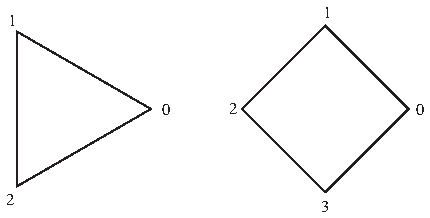
\includegraphics[width=0.590\linewidth,height=.8\textheight,keepaspectratio]{assets/p064_02.pdf}\end{center}
\end{BookFloat}

\noindent We justify calling \BookInline{\langle D_{n},\allowbreak \circ \rangle } a group with Theorem 4.17.

\BookLabel{4.17 Theorem} For any \BookInline{n\geq 3,\allowbreak \langle D_{n},\allowbreak \circ \rangle } is a group.

\BookLabel{\textit{Proof}} We first show that function composition is an operation on \BookInline{D_{n}.} Let \BookInline{\phi,\allowbreak \theta \in D_{n}} and suppose that the line between vertices \BookInline{i} and \BookInline{j} is an edge in \BookInline{P_{n}.} Since \BookInline{\theta \in D_{n},\allowbreak } the line between \BookInline{\theta (i)} and \BookInline{\theta (j)} is an edge of \BookInline{P_{n}.} Because \BookInline{\phi \in D_{n},\allowbreak } and the line between \BookInline{\theta (i)} and \BookInline{\theta (j)} is an edge, the line between \BookInline{\phi (\theta (i))= \phi \circ \theta (i)} and \BookInline{\phi (\theta (j))= \phi \circ \theta (j)} is an edge of \BookInline{P_{n}.}

We leave it to the reader to check that if the line segment between \BookInline{\phi (\theta (i))= \phi \circ \theta (i)} and \BookInline{\phi (\theta (j))= \phi \circ \theta (j)} is an edge of \BookInline{P_{n},\allowbreak } then the line segment between \BookInline{i} and \BookInline{j} is an edge of \BookInline{P_{n}.}

We also know that the composition of one-to-one and onto functions is one-to-one and onto, so \BookInline{\phi \circ \theta \in D_{n}.} Therefore, function composition is an operation on \BookInline{D_{n}.}

The operation of composition of functions is associative, so \BookInline{\mathcal{G}_{1}} is satisfied. The function \BookInline{\iota:\mathbb{Z}_{n}\to \mathbb{Z}_{n}} defined by \BookInline{\iota (k)= k} is an identity in \BookInline{D_{n},\allowbreak } so \BookInline{\mathcal{G}_{2}} is satisfied. Finally, if \BookInline{\phi \in D_{n},\allowbreak } then \BookInline{\phi ^{- 1}\in D_{n};} the inverse function for \BookInline{f} acts as the inverse in the group sense, so \BookInline{\mathcal{G}_{3}} is satisfied. Therefore\BookInline{,\allowbreak \langle D_{n},\allowbreak \circ \rangle } is a group\BookInline{.}\BookEnd{\blacklozenge}

\noindent Following tradition, we will use multiplicative notation in the dihedral groups instead of using \BookInline{\circ.} If the operation on \BookInline{D_{n}} were abelian, we could use additive notation, but in Example 4.18 we find that \BookInline{D_{n}} is not abelian.

\BookLabel{4.18 Example} Let \BookInline{n\geq 3} and \BookInline{\rho:Z_{n}\to Z_{n}} be given by rotating the \BookInline{n-}gon \BookInline{P_{n}} by \BookInline{\frac{2\pi }{n}}, which just rotates each vertex to the next one. That is,

\begin{BookFloat}{04_nonabelian_examples-p64-10}
\begin{center}\small \textbf{4.19 Figure}\end{center}
\begin{center}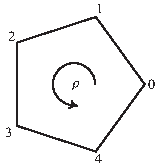
\includegraphics[width=0.220\linewidth,height=.8\textheight,keepaspectratio]{assets/review_v3_p064_4.19.pdf}\end{center}
\end{BookFloat}

\begin{center}\begin{adjustbox}{max width=\linewidth}\BookInline{\displaystyle \rho (k)= k+ _{n}1}\end{adjustbox}\end{center}

\noindent for each \BookInline{k\in \mathbb{Z}_{n},\allowbreak } as can be visualized in Figure 4.19. The function \BookInline{\rho } matches edges to edges and it is one-to-one and onto. So \BookInline{\rho \in D_{n}.}

A second element in \BookInline{D_{n}} is reflection about the \BookInline{x-}axis, which we call \BookInline{\mu.} By glancing at Figure 4.20 we see that in \BookInline{D_{5},\allowbreak \mu (0)= 0,\allowbreak \mu (1)= 4,\allowbreak \mu (2)= 3,\allowbreak \mu (3)= 2,\allowbreak } and \BookInline{\mu (4)= 1.} For any \BookInline{n\geq 3} in general, if \BookInline{k\in \mathbb{Z}_{n},\allowbreak } then

\begin{center}\begin{adjustbox}{max width=\linewidth}\BookInline{\displaystyle \mu (k)= - k.}\end{adjustbox}\end{center}

\noindent (Recall that in \BookInline{\mathbb{Z}_{n},\allowbreak - k} is the additive inverse of \BookInline{k,\allowbreak } which is \BookInline{n- k} for \BookInline{k>0} and \BookInline{- 0= 0.)}

\end{BookBody}

% Source PDF page 65; original printed page 48
\BookSource{65}{48}
\BookNarrativetrue

\begin{BookBody}

Let us check if \BookInline{\mu \rho = \rho \mu.} We start by checking what each function does to 0.

\begin{BookFloat}{04_nonabelian_examples-p65-1}
\begin{center}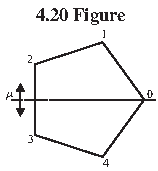
\includegraphics[width=0.217\linewidth,height=.8\textheight,keepaspectratio]{assets/p065_00.pdf}\end{center}
\end{BookFloat}

\begin{center}\begin{adjustbox}{max width=\linewidth}\BookInline{\displaystyle \begin{aligned}\mu (\rho (0))&= \mu (1) \\ &= n- 1\end{aligned}}\end{adjustbox}\end{center}

\begin{center}\begin{adjustbox}{max width=\linewidth}\BookInline{\displaystyle \begin{aligned}\rho (\mu (0))&= \rho (0) \\ &= 1\end{aligned}}\end{adjustbox}\end{center}

\noindent Since \BookInline{n\geq 3,\allowbreak n- 1\neq 1,\allowbreak } which implies that \BookInline{\mu \rho \neq \rho \mu.} Thus for all \BookInline{n\geq 3,\allowbreak D_{n}} is not abelian\BookInline{.}\BookEnd{\blacktriangle}

\BookLabel{4.21 Theorem} Let \BookInline{n\geq 3.} The order of the dihedral group \BookInline{D_{n}} is \BookInline{2n} and

\begin{center}\begin{adjustbox}{max width=\linewidth}\BookInline{\displaystyle D_{n}= \{\iota ,\allowbreak \rho ,\allowbreak \rho ^{2},\allowbreak \rho ^{3},\allowbreak \cdots ,\allowbreak \rho ^{n- 1},\allowbreak \mu ,\allowbreak \mu \rho ,\allowbreak \mu \rho ^{2},\allowbreak \mu \rho ^{3},\allowbreak \cdots ,\allowbreak \mu \rho ^{n- 1}\}.}\end{adjustbox}\end{center}

\BookLabel{\textit{Proof}} We first show there can be at most \BookInline{2n} elements of \BookInline{D_{n}.} If we map the vertices \BookInline{\mathbb{Z}_{n}} to the vertices \BookInline{\mathbb{Z}_{n},\allowbreak } vertex 0 has \BookInline{n} possible images. Let \BookInline{y} be the image of vertex 0. Since \BookInline{y} is connected by an edge to just two vertices, 1 must map to one of these two vertices. So after the image of vertex 0 is determined, there are only two choices for the image of 1. After the images of vertices 0 and 1 are determined, the rest are fixed. This means that there are at most \BookInline{2n} elements of \BookInline{D_{n}.}

To show that \BookInline{|D_{n}|= 2n} we only need to show that no two of the functions \BookInline{\iota = } \BookInline{\rho ^{0},\allowbreak \rho,\allowbreak \rho ^{2},\allowbreak \rho ^{3},\allowbreak...,\allowbreak \rho ^{n- 1},\allowbreak \mu,\allowbreak \mu \rho,\allowbreak \mu \rho ^{2},\allowbreak \mu \rho ^{3},\allowbreak...,\allowbreak \mu \rho ^{n- 1}} are the same. We first suppose that \BookInline{\rho ^{k}= \rho ^{r}} for some integers \BookInline{0\leq k\leq n- 1} and \BookInline{0\leq r\leq n- 1.} Then:

\begin{center}\begin{adjustbox}{max width=\linewidth}\BookInline{\displaystyle \begin{aligned}\rho ^{k}(0)&= \rho ^{r}(0) \\ k+ _{n}0&= r+ _{n}0 \\ k&= r\end{aligned}}\end{adjustbox}\end{center}

\noindent This shows that no two of \BookInline{\iota = \rho ^{0},\allowbreak \rho,\allowbreak \rho ^{2},\allowbreak \rho ^{3},\allowbreak...,\allowbreak \rho ^{n- 1}} are the same.

We next show that no two of \BookInline{\mu = \mu \rho ^{0},\allowbreak \mu \rho,\allowbreak \mu \rho ^{2},\allowbreak \mu \rho ^{3},\allowbreak...,\allowbreak \mu \rho ^{n- 1}} are the same. As before we assume that \BookInline{\mu \rho ^{k}= \mu \rho ^{r}} where \BookInline{0\leq k\leq n- 1} and \BookInline{0\leq r\leq n- 1} are integers. By cancellation, we have \BookInline{\rho ^{k}= \rho ^{r}.} But then \BookInline{k= r} as shown above. Therefore no two of \BookInline{\mu = \mu \rho ^{0},\allowbreak \mu \rho,\allowbreak \mu \rho ^{2},\allowbreak \mu \rho ^{3},\allowbreak...,\allowbreak \mu \rho ^{n- 1}} are the same.

It now only remains to show that there are no values for \BookInline{k} and \BookInline{r} with \BookInline{\rho ^{k}= \mu \rho ^{r}.} Note that traversing the \BookInline{n-}gon in the order

\begin{center}\begin{adjustbox}{max width=\linewidth}\BookInline{\displaystyle \rho ^{k}(0),\allowbreak \rho ^{k}(1),\allowbreak \rho ^{k}(2),\allowbreak \cdots ,\allowbreak \rho ^{k}(n- 1)}\end{adjustbox}\end{center}

\noindent progresses in a counterclockwise manner regardless of which \BookInline{k} we use. On the other hand,

\begin{center}\begin{adjustbox}{max width=\linewidth}\BookInline{\displaystyle \mu \rho ^{k}(0),\allowbreak \mu \rho ^{k}(1),\allowbreak \mu \rho ^{k}(3),\allowbreak \cdots ,\allowbreak \mu \rho ^{k}(n)}\end{adjustbox}\end{center}

\noindent traverses the \BookInline{n-}gon in a clockwise manner. This shows that there are no values of \BookInline{k} and \BookInline{r} for which \BookInline{\rho ^{k}= \mu \rho ^{r}.} Therefore\BookInline{,\allowbreak D_{n}} has at least \BookInline{2n} elements. Combining this with the fact that \BookInline{D_{n}} has at most \BookInline{2n} elements shows that \BookInline{|D_{n}|= 2n} and

\begin{center}\begin{adjustbox}{max width=\linewidth}\BookInline{\displaystyle D_{n}= \{\iota ,\allowbreak \rho ,\allowbreak \rho ^{2},\allowbreak \rho ^{3},\allowbreak \cdots ,\allowbreak \rho ^{n- 1},\allowbreak \mu ,\allowbreak \mu \rho ,\allowbreak \mu \rho ^{2},\allowbreak \mu \rho ^{3},\allowbreak \cdots ,\allowbreak \mu \rho ^{n- 1}\}.}\end{adjustbox}\end{center} \BookEnd{\blacklozenge}

\noindent Theorem 4.21 says that if \BookInline{\phi \in D_{n},\allowbreak } then there is an integer \BookInline{0\leq k\leq n- 1} such that either \BookInline{\phi = \rho ^{k}} or else \BookInline{\phi = \mu \rho ^{k}.} We refer to this representation of \BookInline{\phi } as the\textbf{ standard form}. We notice that each application of \BookInline{\mu } reverses the direction traversed by the images of \BookInline{0,\allowbreak 1,\allowbreak 2,\allowbreak 3,\allowbreak...,\allowbreak n.} We use this fact in the following example.

\BookLabel{4.22 Example} Let \BookInline{n\geq 3.} We know \BookInline{\rho \mu \neq \mu \rho } from Example 4.18, so let us determine \BookInline{\rho \mu \in D_{n}} in standard form. Each time we apply \BookInline{\mu } we reverse the clock direction of the images of \BookInline{0,\allowbreak 1,\allowbreak 2,\allowbreak 3,\allowbreak...,\allowbreak n- 1.} This means that \BookInline{\mu \rho \mu } reverses direction twice, so the rotation is 
% Source PDF page 66; original printed page 49
\BookSource{66}{49}
back to counterclockwise. Thus \BookInline{\mu \rho \mu = \rho ^{k}} for some \BookInline{k.} We determine the value of \BookInline{k} by determining where 0 is sent:

\end{BookBody}

\BookNarrativetrue

\begin{BookBody}

\begin{center}\begin{adjustbox}{max width=\linewidth}\BookInline{\displaystyle k= \rho ^{k}(0)= \mu \rho \mu (0)= \mu \rho (0)= \mu (1)= n- 1}\end{adjustbox}\end{center}

Therefore,

\begin{center}\begin{adjustbox}{max width=\linewidth}\BookInline{\displaystyle \mu \rho \mu = \rho ^{n- 1}.}\end{adjustbox}\end{center}

\noindent Multiplying both sides on the left by \BookInline{\mu } yields:

\begin{center}\begin{adjustbox}{max width=\linewidth}\BookInline{\displaystyle \mu \mu \rho \mu = \mu \rho ^{n- 1}}\end{adjustbox}\end{center}

\noindent Since \BookInline{\mu \mu = \iota,\allowbreak } we conclude that

\begin{center}\begin{adjustbox}{max width=\linewidth}\BookInline{\displaystyle \rho \mu = \mu \rho ^{n- 1}.}\end{adjustbox}\end{center} \BookEnd{\blacktriangle}

\noindent When computing products in \BookInline{D_{n}} we normally want our answer in standard form. This is not difficult if we keep in mind a few basic facts about the group \BookInline{D_{n}.} We have shown some of the properties listed below, and the rest you will be asked to verify in the exercises.

\noindent \BookInline{1.\rho ^{n}= \iota (}Rotation by \BookInline{2\pi } is the identity map.)

\noindent \BookInline{2.(\rho ^{k})^{- 1}= \rho ^{n- k}}

\noindent \BookInline{3.\mu ^{2}= \iota,\allowbreak } which implies \BookInline{\mu ^{- 1}= \mu (}Reflect across a line twice is the identity map.) \BookInline{4.\rho ^{k}\mu = \mu \rho ^{n- k}(}Example 4.22 for \BookInline{k= 1} and Exercise 30 for any \BookInline{k.)}

\BookLabel{4.23 Example} In the group \BookInline{D_{5}} compute \BookInline{(\mu \rho ^{2})(\mu \rho ).} We see that

\begin{center}\begin{adjustbox}{max width=\linewidth}\BookInline{\displaystyle \begin{aligned}(\mu \rho ^{2})(\mu \rho )&= \mu \rho ^{2}\mu \rho  \\ &= \mu (\rho ^{2}\mu )\rho  \\ &= \mu (\mu \rho ^{5- 2})\rho  \\ &= \mu ^{2}\rho ^{4} \\ &= \rho ^{4}\end{aligned}}\end{adjustbox}\end{center} \BookEnd{\blacktriangle}

\BookLabel{4.24 Example} In the dihedral group \BookInline{D_{n}} compute \BookInline{(\mu \rho ^{k})^{- 1}.}

\begin{center}\begin{adjustbox}{max width=\linewidth}\BookInline{\displaystyle \begin{aligned}(\mu \rho ^{k})^{- 1}&= (\rho ^{k})^{- 1}\mu ^{- 1} \\ &= \rho ^{n- k}\mu  \\ &= \mu \rho ^{n- (n- k)} \\ &= \mu \rho ^{k}\end{aligned}}\end{adjustbox}\end{center} \BookEnd{\blacktriangle}

\noindent In Example 4.24 we determined that the inverse of \BookInline{\mu \rho ^{k}} is itself, which suggests that \BookInline{\mu \rho ^{k}} could be reflection across a line of symmetry. In Exercise 37, you will be asked to show this is the case. Geometrically, we can see that each of the elements of the form \BookInline{\mu \rho ^{k}} is reflection across a line. Placing one mirror along the line of reflection for \BookInline{\mu } and another mirror along the line of reflection for \BookInline{\mu \rho } is the basis for designing a kaleidoscope. Any element in \BookInline{D_{n}} can be written as a product using only the elements \BookInline{\mu } and \BookInline{\mu \rho } since we can write \BookInline{\rho = \mu \mu \rho.} In a kaleidoscope successive reflections across the mirrors correspond to taking products involving \BookInline{\mu } and \BookInline{\mu \rho.} So the image you see in the kaleidoscope has all the symmetries in \BookInline{D_{n}.} That is, you can rotate the image by \BookInline{\frac{360^{\circ }}{n}} or reflect it across any one of the lines of reflection for the elements \BookInline{\mu \rho ^{k}.} Figure 4.25 is a typical image from a kaleidoscope with dihedral group \BookInline{D_{16}} symmetries.

\end{BookBody}

% Source PDF page 67; original printed page 50
\BookSource{67}{50}
\BookNarrativefalse

\begin{BookBody}

\begin{BookFloat}{04_nonabelian_examples-p67-0}
\begin{center}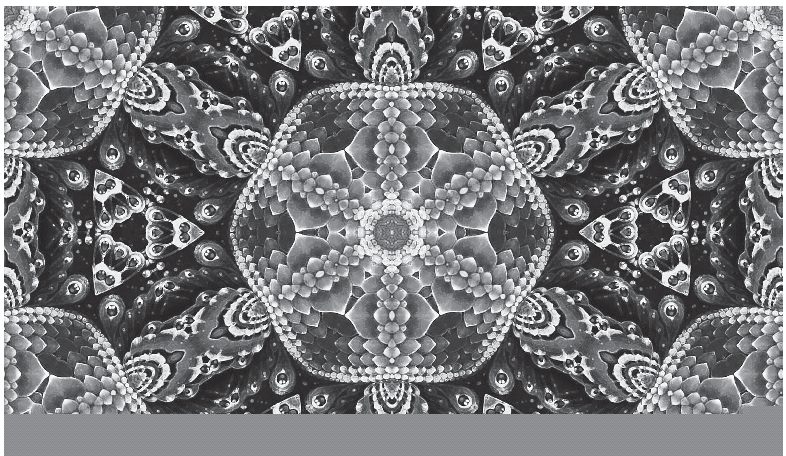
\includegraphics[width=1.000\linewidth,height=.8\textheight,keepaspectratio]{assets/p067_00.pdf}\end{center}
\begin{center}\small\textbf{4.25 Figure}\end{center}
\end{BookFloat}

k c o t s r e t t u h S / n o i t a e r c \_ I Z I

\BookExerciseTitle{4} \BookEnd{\blacksquare}

\BookTextHeading{\textbf{Computation}}

\noindent In Exercises 1 through 5, compute the indicated product involving the following permutations in \BookInline{S_{6}:} \BookInline{\sigma = \begin{pmatrix}1 & 2 & 3 & 4 & 5 & 6 \\3 & 1 & 4 & 5 & 6 & 2\end{pmatrix}}, \BookInline{\tau = \begin{pmatrix}1 & 2 & 3 & 4 & 5 & 6 \\2 & 4 & 1 & 3 & 6 & 5\end{pmatrix}}, \BookInline{\mu = \begin{pmatrix}1 & 2 & 3 & 4 & 5 & 6 \\5 & 2 & 4 & 3 & 1 & 6\end{pmatrix}}.

\BookExercise{1.}{\BookInline{\tau \sigma }}

\BookExercise{2.}{\BookInline{\tau ^{2}\sigma }}

\BookExercise{3.}{\BookInline{\mu \sigma ^{2}}}

\BookExercise{4.}{\BookInline{\sigma ^{- 2}\tau }}

\BookExercise{5.}{\BookInline{\sigma ^{- 1}\tau \sigma }}

\noindent In Exercises 6 through 9, compute the expressions shown for the permutations \BookInline{\sigma,\allowbreak \tau,\allowbreak } and \BookInline{\mu } defined prior to Exercise 1.

\BookExercise{6.}{\BookInline{\sigma ^{6}}}

\BookExercise{7.}{\BookInline{\mu ^{2}}}

\BookExercise{8.}{100 \BookInline{\sigma }}

\BookExercise{9.}{100 \BookInline{\mu }}

\BookExercise{10.}{Convert the permutations \BookInline{\sigma,\allowbreak \tau,\allowbreak } and \BookInline{\mu } defined prior to Exercise 1 to disjoint cycle notation.}

\BookExercise{11.}{Convert the following permutations in \BookInline{S_{8}} from disjoint cycle notation to two-row notation. \textbf{a.} (1, 4, 5)(2, 3) \textbf{b.} (1, 8, 5)(2, 6, 7, 3, 4) \textbf{c.} (1, 2, 3)(4, 5)(6, 7, 8)}

\BookExercise{12.}{Compute the permutation products. \textbf{a.} (1, 5, 2, 4)(1, 5, 2, 3) \textbf{b}\BookInline{.(1,\allowbreak 5,\allowbreak 3)(1,\allowbreak 2,\allowbreak 3,\allowbreak 4,\allowbreak 5,\allowbreak 6)(1,\allowbreak 5,\allowbreak 3)^{- 1}} \textbf{c}\BookInline{.[(1,\allowbreak 6,\allowbreak 7,\allowbreak 2)^{2}(4,\allowbreak 5,\allowbreak 2,\allowbreak 6)^{- 1}(1,\allowbreak 7,\allowbreak 3)]^{- 1}} \textbf{d.} (1, 6)(1, 5)(1, 4)(1, 3)(1, 2)}

\BookExercise{13.}{Compute the following elements of \BookInline{D_{12}.} Write your answer in standard form. \textbf{a}\BookInline{.\mu \rho ^{2}\mu \rho ^{8}} \textbf{b}\BookInline{.\mu \rho ^{10}\mu \rho ^{- 1}} \textbf{c}\BookInline{.\rho \mu \rho ^{- 1}} \textbf{d}\BookInline{.(\mu \rho ^{3}\mu ^{- 1}\rho ^{- 1})^{- 1}}}

\end{BookBody}

% Source PDF page 68; original printed page 51
\BookSource{68}{51}
\BookNarrativefalse

\begin{BookBody}

\BookExercise{14.}{Write the group table for \BookInline{D_{3}.} Compare the group tables for \BookInline{D_{3}} and \BookInline{S_{3}.} Are the groups isomorphic?}

Let \BookInline{A} be a set and let \BookInline{\sigma \in S_{A}.} For a fixed \BookInline{a\in A,\allowbreak } the set

\begin{center}\begin{adjustbox}{max width=\linewidth}\BookInline{\displaystyle \mathcal{O}_{a,\allowbreak \sigma }= \{\sigma ^{n}(a)\mid n\in \mathbb{Z}\}}\end{adjustbox}\end{center}

is the\textbf{ orbit} of \BookInline{a} \textbf{under} \BookInline{\sigma.} In Exercises 15 through 17, find the orbit of 1 under the permutation defined prior to Exercise 1.

\BookExercise{15.}{\BookInline{\sigma }}

\BookExercise{16.}{\BookInline{\tau }}

\BookExercise{17.}{\BookInline{\mu }}

\BookExercise{18.}{Verify that \BookInline{H= \{\iota,\allowbreak \mu,\allowbreak \rho ^{2},\allowbreak \mu \rho ^{2}\}\subseteq D_{4}} is a group using the operation function composition.}

\BookExercise{19.}{\textbf{. a} Verify that the six matrices}

\begin{center}\begin{adjustbox}{max width=\linewidth}\BookInline{\displaystyle \begin{bmatrix} 1 & 0 & 0 \\ 0 & 1 & 0 \\ 0 & 0 & 1 \end{bmatrix},\allowbreak  \begin{bmatrix} 0 & 1 & 0 \\ 0 & 0 & 1 \\ 1 & 0 & 0 \end{bmatrix},\allowbreak  \begin{bmatrix} 0 & 0 & 1 \\ 1 & 0 & 0 \\ 0 & 1 & 0 \end{bmatrix},\allowbreak  \begin{bmatrix} 1 & 0 & 0 \\ 0 & 0 & 1 \\ 0 & 1 & 0 \end{bmatrix},\allowbreak  \begin{bmatrix} 0 & 0 & 1 \\ 0 & 1 & 0 \\ 1 & 0 & 0 \end{bmatrix},\allowbreak  \begin{bmatrix} 0 & 1 & 0 \\ 1 & 0 & 0 \\ 0 & 0 & 1 \end{bmatrix}}\end{adjustbox}\end{center}

form a group under matrix multiplication. [\textit{Hint}: Don’t try to compute all products of these matrices. Instead, think how the column vector \BookInline{\begin{bmatrix} 0 \\ 1 \\ 2 \end{bmatrix}} is transformed by multiplying it on the left by each of the matrices.]

\BookExercise{b.}{What group discussed in this section is isomorphic to this group of six matrices?}

\BookExercise{20.}{After working Exercise 18, write down eight matrices that form a group under matrix multiplication that is isomorphic to \BookInline{D_{4}.}}

\BookTextHeading{\textbf{Concepts}}

\noindent In Exercises 21 through 23, correct the definition of the italicized term without reference to the text, if correction is needed, so that it is in a form acceptable for publication.

\BookExercise{21.}{The\textit{ dihedral group} \BookInline{D_{n}} is the set of all functions \BookInline{\phi:\mathbb{Z}_{n}\to \mathbb{Z}_{n}} such that the line segment between vertex \BookInline{i} and vertex \BookInline{j} of \BookInline{U_{n}} is an edge of \BookInline{P_{n}} if and only if the line segment between vertices \BookInline{\phi (i)} and \BookInline{\phi (j)} in \BookInline{U_{n}} is an edge of \BookInline{P_{n}.}}

\BookExercise{22.}{A\textit{ permutation} of a set \BookInline{S} is a one-to-one map from \BookInline{S} to \BookInline{S.}}

\BookExercise{23.}{The\textit{ order} of a group is the number of elements in the group.}

\noindent In Exercises 24 through 28, determine whether the given function is a permutation of \BookInline{\mathbb{R}.}

\BookExercise{24.}{\BookInline{f_{1}:\mathbb{R}\to \mathbb{R}} defined by \BookInline{f_{1}(x)= x+ 1}}

\BookExercise{25.}{\BookInline{f_{2}:\mathbb{R}\to \mathbb{R}} defined by \BookInline{f_{2}(x)= x^{2}}}

\BookExercise{26.}{\BookInline{f_{3}:\mathbb{R}\to \mathbb{R}} defined by \BookInline{f_{3}(x)= - x^{3}}}

\BookExercise{27.}{\BookInline{f_{4}:\mathbb{R}\to \mathbb{R}} defined by \BookInline{f_{4}(x)= e^{x}}}

\BookExercise{28.}{\BookInline{f_{5}:\mathbb{R}\to \mathbb{R}} defined by \BookInline{f_{5}(x)= x^{3}- x^{2}- 2x}}

\BookExercise{29.}{Determine whether each of the following is true or false.}

\BookExercise{a.}{Every permutation is a one-to-one function.}

\BookExercise{b.}{Every function is a permutation if and only if it is one-to-one.}

\BookExercise{c.}{Every function from a finite set onto itself must be one-to-one.}

\BookExercise{d.}{Every subset of an abelian group \BookInline{G} that is also a group using the same operation as \BookInline{G} is abelian.}

\BookExercise{e.}{The symmetric group \BookInline{S_{10}} has 10 elements.}

\BookExercise{f.}{If \BookInline{\phi \in D_{n},\allowbreak } then \BookInline{\phi } is a permutation on the set \BookInline{\mathbb{Z}_{n}.}}

\BookExercise{g.}{The group \BookInline{D_{n}} has exactly \BookInline{n} elements.}

\BookExercise{h.}{\textbf{h}\BookInline{.D_{3}} is a subset of \BookInline{D_{4}.}}

\BookTextHeading{\textbf{Theory}}

\BookExercise{30.}{Let \BookInline{n\geq 3} and \BookInline{k\in \mathbb{Z}_{n}.} Prove that in \BookInline{D_{n},\allowbreak \rho ^{k}\mu = \mu \rho ^{n- k}.}}

\BookExercise{31.}{Show that \BookInline{S} is a nonabelian group for \BookInline{n\geq 3.}}

\end{BookBody}

% Continuation on source PDF page 69, preceding Section 5
\BookNarrativefalse

\begin{BookBody}

\BookExercise{32.}{Strengthening Exercise 31, show that if \BookInline{n\geq 3,\allowbreak } then the only element of \BookInline{\sigma } of \BookInline{S_{n}} satisfying \BookInline{\sigma \gamma = \gamma \sigma } for all \BookInline{\gamma \in S_{n}} is \BookInline{\sigma = \iota,\allowbreak } the identity permutation.}

\BookExercise{33.}{Orbits were defined before Exercise 15. Let \BookInline{a,\allowbreak b\in A} and \BookInline{\sigma \in S_{A}.} Show that if \BookInline{\mathcal{O}_{a,\allowbreak \sigma }} and \BookInline{\mathcal{O}_{b,\allowbreak \sigma }} have an element in common, then \BookInline{\mathcal{O}_{a,\allowbreak \sigma }= \mathcal{O}_{b,\allowbreak \sigma }.}}

\BookExercise{34.}{(See the warning following Theorem 4.8.) Let \BookInline{G} be a group with binary operation \BookInline{\ast.} Let \BookInline{G^{\prime }} be the same set as \BookInline{G,\allowbreak } and define a binary operation \BookInline{\ast ^{\prime }} on \BookInline{G^{\prime }} by \BookInline{x\ast ^{\prime }y= y\ast x} for all \BookInline{x,\allowbreak y\in G^{\prime }.}}

\BookExercise{a.}{(Intuitive argument that \BookInline{G^{\prime }} under \BookInline{\ast ^{\prime }} is a group.) Suppose the front wall of your classroom were made of transparent glass, and that all possible products \BookInline{a\ast b= c} and all possible instances \BookInline{a\ast (b\ast c)= } \BookInline{(a\ast b)\ast c} of the associative property for \BookInline{G} under \BookInline{\ast } were written on the wall with a magic marker. What would a person see when looking at the other side of the wall from the next room in front of yours?}

\BookExercise{b.}{Show from the mathematical definition of \BookInline{\ast ^{\prime }} that \BookInline{G^{\prime }} is a group under \BookInline{\ast ^{\prime }.}}

\BookExercise{35.}{Give a careful proof using the definition of isomorphism that if \BookInline{G} and \BookInline{G^{\prime }} are both groups with \BookInline{G} abelian and \BookInline{G^{\prime }} not abelian, then \BookInline{G} and \BookInline{G^{\prime }} are not isomorphic.}

\BookExercise{36.}{Prove that for any integer \BookInline{n\geq 2,\allowbreak } there are at least two nonisomorphic groups with exactly \BookInline{2n} elements.}

\BookExercise{37.}{Let \BookInline{n\geq 3} and \BookInline{0\leq k\leq n- 1.} Prove that the map \BookInline{\mu \rho ^{k}\in D_{n}} is reflection about the line through the origin that makes an angle of \BookInline{- \frac{\pi k}{n}} with the \BookInline{x- }axis.}

\BookExercise{38.}{Let \BookInline{n\geq 3} and \BookInline{k,\allowbreak r\in \mathbb{Z}_{n}.} Based on Exercise 37, determine the element of \BookInline{D_{n}} that corresponds to first reflecting across the line through the origin at an angle of \BookInline{- \frac{2\pi k}{n}} and then reflection across the line through the origin making an angle of \BookInline{- \frac{2\pi r}{n}.} Prove your answer.}

\end{BookBody}
\ifdefined\BookMaster\let\BookFinish\relax\else\def\BookFinish{\end{document}}\fi\BookFinish

\clearpage
% !TeX program = xelatex
\ifdefined\BookMaster\else
\documentclass[11pt,oneside]{article}
% !TeX program = xelatex
\usepackage[b5paper,left=22mm,right=22mm,top=20mm,bottom=22mm,footskip=11mm]{geometry}
\usepackage{fontspec}
\setmainfont{TeX Gyre Termes}
\setsansfont{TeX Gyre Heros}
\usepackage{amsmath,amssymb,mathtools,amsthm}
\renewcommand{\cdots}{\mathinner{\cdotp\cdotp\cdotp}}
\usepackage{graphicx,adjustbox,array,booktabs,longtable,multirow,enumitem,changepage,needspace}
\usepackage[table]{xcolor}
\usepackage{fancyhdr}
\raggedbottom
\interfootnotelinepenalty=10000
\newcommand{\BookFootnote}[2]{\begingroup\renewcommand{\thefootnote}{\fnsymbol{footnote}}\footnote[#1]{#2}\endgroup}
\newcommand{\BookFootnoteMark}[1]{\begingroup\renewcommand{\thefootnote}{\fnsymbol{footnote}}\footnotemark[#1]\endgroup}
\newcommand{\BookFootnoteText}[2]{\begingroup\renewcommand{\thefootnote}{\fnsymbol{footnote}}\footnotetext[#1]{#2}\endgroup}
\newenvironment{BookFloat}[1]{\par\addvspace{.6\baselineskip}\noindent\def\BookFloatID{#1}\begin{minipage}{\linewidth}\phantomsection\label{bookfloat:#1:start}}{\phantomsection\label{bookfloat:\BookFloatID:end}\end{minipage}\par\addvspace{.6\baselineskip}}

\usepackage[unicode,hidelinks]{hyperref}
\pagestyle{fancy}
\fancyhf{}
\newcommand{\BookFooter}{}
\fancyfoot[L]{\parbox[b]{\dimexpr\textwidth-15mm}{\footnotesize\BookFooter}}
\fancyfoot[R]{\footnotesize\thepage}
\renewcommand{\headrulewidth}{0pt}
\renewcommand{\footrulewidth}{0pt}
\setlength{\parindent}{0pt}
\setlength{\parskip}{0.2em}
\setlength{\emergencystretch}{3em}
\setlist{nosep,leftmargin=1.7em,labelsep=.65em}
\newif\ifBookNarrative
\BookNarrativetrue
\newenvironment{BookBody}{\setlength{\parindent}{0pt}}{}
\newcommand{\BookStatement}[1]{\par\addvspace{.6\baselineskip}\noindent #1\enspace\ignorespaces}
\newcommand{\BookLabel}[1]{\par\addvspace{.6\baselineskip}\needspace{3\baselineskip}\noindent\textbf{#1}\quad\ignorespaces}
\newcommand{\BookHeading}[1]{\par\addvspace{\baselineskip}\needspace{4\baselineskip}\noindent{\large\bfseries #1}\par\medskip}
\newcommand{\BookSubheading}[1]{\par\addvspace{.7\baselineskip}\needspace{3\baselineskip}\noindent{\bfseries #1}\par\smallskip}
\newcommand{\BookTextHeading}[1]{\par\addvspace{.7\baselineskip}\needspace{3\baselineskip}\noindent #1\par\smallskip}
\newcommand{\BookSectionTitle}[2]{\par\addvspace{1.2\baselineskip}\needspace{5\baselineskip}\noindent\colorbox{gray!25}{\sffamily\bfseries\small SECTION #1}\quad{\large\bfseries #2}\par\medskip}
\newcommand{\BookExerciseTitle}[1]{\par\addvspace{\baselineskip}\needspace{4\baselineskip}\noindent{\color{gray}\rule{1.5mm}{1.5mm}}\enspace{\large\bfseries Exercises #1}\par\medskip}
\newcommand{\BookBullet}[1]{\begin{list}{\textbullet}{\setlength{\leftmargin}{1.7em}\setlength{\labelwidth}{1em}\setlength{\labelsep}{.7em}\setlength{\topsep}{0pt}\setlength{\parsep}{0pt}\setlength{\itemsep}{0pt}}\item #1\end{list}}
\newcommand{\BookExercise}[2]{\begin{list}{\textbf{#1}}{\setlength{\leftmargin}{2.2em}\setlength{\labelwidth}{1.5em}\setlength{\labelsep}{.7em}\setlength{\topsep}{.15em}\setlength{\parsep}{0pt}\setlength{\itemsep}{0pt}}\item #2\end{list}}
\newcommand{\BookEnd}[1]{\unskip\nobreak\hfill\ensuremath{#1}}
\newcommand{\BookSource}[2]{\phantomsection\label{sourcepage:#1}} % Source-page anchors, retained through reflow.
\usepackage{multicol}
\usepackage{tikz}
\newcommand{\BookPartEntry}[2]{\par\noindent\makebox[17mm][l]{\bfseries Section #1}#2\par}
\newcommand{\BookPartTitle}[3]{\par\bigskip\noindent\begin{tikzpicture}\node[anchor=north west,inner sep=0pt,outer sep=0pt] (bookpart) at (0,0) {\begin{minipage}{\dimexpr\linewidth-.5pt}\hspace*{26mm}\begin{minipage}[t]{\dimexpr\linewidth-26mm}\begin{adjustbox}{max width=\linewidth}{\fontsize{20}{24}\selectfont\bfseries #2}\end{adjustbox}\par\vspace{6mm}\hrule\vspace{6mm}{\sffamily\footnotesize\setlength{\parskip}{.3em}#3}\vspace{3mm}\end{minipage}\end{minipage}};\path[shade,top color=gray!60,bottom color=white] (0,0) rectangle ([xshift=24mm]bookpart.south west);\node[anchor=north,font=\sffamily\bfseries\small] at (12mm,-2mm) {PART};\node[anchor=north,font=\sffamily\bfseries\Huge] at (12mm,-7mm) {#1};\end{tikzpicture}\par\bigskip}
\newsavebox{\BookMathBox}
\makeatletter
\newcommand{\BookInline}[1]{\leavevmode\hskip0pt\relax\begingroup\in@{\begin}{#1}\ifin@\sbox{\BookMathBox}{\(#1\)}\ifdim\wd\BookMathBox>\dimexpr\linewidth-1em\relax\resizebox{\dimexpr\linewidth-1em\relax}{!}{\usebox{\BookMathBox}}\else\(#1\)\fi\else\in@{\left}{#1}\ifin@\sbox{\BookMathBox}{\(#1\)}\ifdim\wd\BookMathBox>\dimexpr\linewidth-1em\relax\resizebox{\dimexpr\linewidth-1em\relax}{!}{\usebox{\BookMathBox}}\else\(#1\)\fi\else\(#1\)\fi\fi\endgroup\hskip0pt\relax}
\makeatother
\DeclareMathOperator{\Aut}{Aut}
\DeclareMathOperator{\End}{End}
\DeclareMathOperator{\Hom}{Hom}
\DeclareMathOperator{\GF}{GF}
\DeclareMathOperator{\irr}{irr}
\DeclareMathOperator{\lt}{lt}
\DeclareMathOperator{\lp}{lp}
\providecommand{\textcircled}[1]{\textnormal{(#1)}}

\begin{document}
\fi
\renewcommand{\BookFooter}{Section 5 Subgroups}
\pdfbookmark[0]{Section 5 Subgroups}{05_subgroups}
\ifdefined\BookMaster\else\setcounter{page}{52}\fi
% Source PDF page 69; original printed page 52
\BookSource{69}{52}
\BookNarrativetrue

\begin{BookBody}

\BookSectionTitle{5}{Subgroups}

\BookTextHeading{\textbf{Subsets and Subgroups}  }

\noindent You may have noticed that we sometimes have had groups contained within larger groups. For example, the group \BookInline{\mathbb{Z}} under addition is contained within the group \BookInline{\mathbb{Q}} under addition, which in turn is contained in the group \BookInline{\mathbb{R}} under addition. When we view the group \BookInline{\langle \mathbb{Z},\allowbreak + \rangle } as contained in the group \BookInline{\langle \mathbb{R},\allowbreak + \rangle,\allowbreak } it is very important to notice that the operation \BookInline{+ } on integers \BookInline{n} and \BookInline{m} as elements of \BookInline{\langle \mathbb{Z},\allowbreak + \rangle } produces the same element \BookInline{n+ m} as would result if you were to think of \BookInline{n} and \BookInline{m} as elements in \BookInline{\langle \mathbb{R},\allowbreak + \rangle.} Thus we should \textit{not} regard the group \BookInline{\langle \mathbb{Q}^{+ },\allowbreak \cdot \rangle } as contained in \BookInline{\langle \mathbb{R},\allowbreak + \rangle,\allowbreak } even though \BookInline{\mathbb{Q}^{+ }} is contained in \BookInline{\mathbb{R}} as a set. In this instance\BookInline{,\allowbreak 2\cdot 3= 6} in \BookInline{\langle \mathbb{Q}^{+ },\allowbreak \cdot \rangle,\allowbreak } while \BookInline{2+ 3= 5} in \BookInline{\langle \mathbb{R},\allowbreak + \rangle.} We are requiring not only that the set of one group be a subset of the set of the other, but also that the group operation on the subset be the\textit{ induced operation} that assigns the same element to each ordered pair from this subset as is assigned by the group operation on the whole set.

\BookLabel{5.1 Definition} If a subset \BookInline{H} of a group \BookInline{G} is closed under the binary operation of \BookInline{G} and if \BookInline{H} with the induced operation from \BookInline{G} is itself a group, then \BookInline{H} is a\textbf{ subgroup of} \BookInline{G.} We shall let \BookInline{H\leq G} or \BookInline{G\geq H} denote that \BookInline{H} is a subgroup of \BookInline{G,\allowbreak } and \BookInline{H<G} or \BookInline{G>H} shall mean \BookInline{H\leq G} but \BookInline{H\neq G.}\BookEnd{\blacksquare}

Thus \BookInline{\langle \mathbb{Z},\allowbreak + \rangle <\langle \mathbb{R},\allowbreak + \rangle } but \BookInline{\langle \mathbb{Q}^{+ },\allowbreak \cdot \rangle } is\textit{ not} a subgroup of \BookInline{\langle \mathbb{R},\allowbreak + \rangle,\allowbreak } even though as sets, \BookInline{\mathbb{Q}^{+ }\subset \mathbb{R}.} Every group \BookInline{G} has as subgroups \BookInline{G} itself and \BookInline{\{e\},\allowbreak } where \BookInline{e} is the identity element of \BookInline{G.}

\BookLabel{5.2 Definition} If \BookInline{G} is a group, then the subgroup consisting of \BookInline{G} itself is the\textbf{ improper subgroup} of \BookInline{G.} All other subgroups are\textbf{ proper subgroups}. The subgroup \BookInline{\{e\}} is the\textbf{ trivial subgroup} of \BookInline{G.} All other subgroups are\textbf{ nontrivial}\BookInline{.}\BookEnd{\blacksquare}

\noindent We turn to some illustrations.

\end{BookBody}

% Source PDF page 70; original printed page 53
\BookSource{70}{53}
\BookNarrativetrue

\begin{BookBody}

\BookLabel{5.3 Example} Let \BookInline{\mathbb{R}^{n}} be the additive group of all \BookInline{n-}component row vectors with real number entries. The subset consisting of all of these vectors having 0 as entry in the first component is a subgroup of \BookInline{\mathbb{R}^{n}.}\BookEnd{\blacktriangle}

\BookLabel{5.4 Example} \BookInline{\mathbb{Q}^{+ }} under multiplication is a proper subgroup of \BookInline{\mathbb{R}^{+ }} under multiplication. \BookEnd{\blacktriangle}

\BookLabel{5.5 Example} The \BookInline{n}\textbf{th} roots of unity in \BookInline{\mathbb{C},\allowbreak U_{n},\allowbreak } form a subgroup of \BookInline{U,\allowbreak } the complex numbers whose absolute value is 1, which in turn is a subgroup of \BookInline{\mathbb{C}^{\ast },\allowbreak } the nonzero complex numbers under multiplication\BookInline{.}\BookEnd{\blacktriangle}

\BookLabel{5.6 Example} Recall that \BookInline{S_{\mathbb{Z}_{n}}} is the set of all one-to-one functions mapping \BookInline{\mathbb{Z}_{n}} onto \BookInline{\mathbb{Z}_{n}} and \BookInline{D_{n}} is the set of all one-to-one functions \BookInline{\phi } mapping \BookInline{\mathbb{Z}_{n}} onto \BookInline{\mathbb{Z}_{n}} with the further property that the line segment between \BookInline{i} and \BookInline{j} is an edge of the regular \BookInline{n-}gon \BookInline{P_{n}} if and only if the line segment between \BookInline{\phi (i)} and \BookInline{\phi (j)} is an edge. \BookInline{D_{n}\subseteq S_{\mathbb{Z}_{n}}}. Since both \BookInline{D_{n}} and \BookInline{S_{\mathbb{Z}_{n}}} are groups under composition of functions, \BookInline{D_{n}\leq S_{\mathbb{Z}_{n}}} \BookInline{.}\BookEnd{\blacktriangle}

\BookLabel{5.7 Example} There are two different types of group structures of order 4 (see Exercise 20 of Section 2). We describe them by their group tables (Tables 5.8 and 5.9). The group \BookInline{V} is the Klein 4-group.

The only nontrivial proper subgroup of \BookInline{\mathbb{Z}_{4}} is \BookInline{\{0,\allowbreak 2\}.} Note that \BookInline{\{0,\allowbreak 3\}} is\textit{ not} a subgroup of \BookInline{\mathbb{Z}_{4},\allowbreak } since \BookInline{\{0,\allowbreak 3\}} is\textit{ not closed} under \BookInline{+.} For example\BookInline{,\allowbreak 3+ 3= 2,\allowbreak } and \BookInline{2\notin \{0,\allowbreak 3\}.} However, the group \BookInline{V} has three nontrivial proper subgroups\BookInline{,\allowbreak \{e,\allowbreak a\},\allowbreak \{e,\allowbreak b\},\allowbreak } and \BookInline{\{e,\allowbreak c\}.} Here \BookInline{\{e,\allowbreak a,\allowbreak b\}} is\textit{ not} a subgroup, since \BookInline{\{e,\allowbreak a,\allowbreak b\}} is not closed under the operation of \BookInline{V} because \BookInline{ab= c,\allowbreak } and \BookInline{c\notin \{e,\allowbreak a,\allowbreak b\}.}\BookEnd{\blacktriangle}

\begin{BookFloat}{05_subgroups-p70-7}
\begin{center}
\begin{minipage}[t]{0.4917\linewidth}\vspace{0pt}\begin{center}\small\textbf{5.8 Table}\end{center}
\begin{center}\begin{adjustbox}{max width=\linewidth}
\renewcommand{\arraystretch}{1.2}\setlength{\tabcolsep}{5pt}
\begin{tabular}{c|c|c|c|c}
\BookInline{\mathbb{Z}_{4}:+ } & 0 & 1 & 2 & 3\\\hline
0 & 0 & 1 & 2 & 3\\\hline
1 & 1 & 2 & 3 & 0\\\hline
2 & 2 & 3 & 0 & 1\\\hline
3 & 3 & 0 & 1 & 2\\
\end{tabular}
\end{adjustbox}\end{center}\end{minipage}\hfill\begin{minipage}[t]{0.4444\linewidth}\vspace{0pt}\begin{center}\small\textbf{5.9 Table}\end{center}
\begin{center}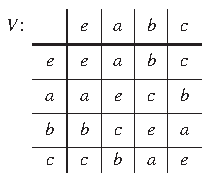
\includegraphics[width=\linewidth,height=.8\textheight,keepaspectratio]{assets/p070_09.pdf}\end{center}\end{minipage}
\end{center}
\end{BookFloat}

It is often useful to draw a\textit{ subgroup diagram} of the subgroups of a group. In such a diagram, a line running downward from a group \BookInline{G} to a group \BookInline{H} means that \BookInline{H} is a subgroup of \BookInline{G.} Thus the larger group is placed nearer the top of the diagram. Figure 5.10 contains the subgroup diagrams for the groups \BookInline{\mathbb{Z}_{4}} and \BookInline{V} of Example 5.7.

\begin{BookFloat}{05_subgroups-p70-9}
\begin{center}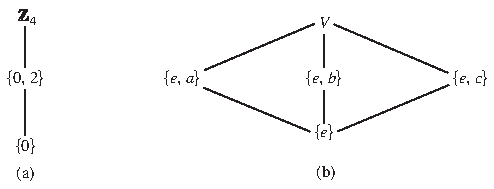
\includegraphics[width=0.677\linewidth,height=.8\textheight,keepaspectratio]{assets/p070_11.pdf}\end{center}
\begin{center}\small\textbf{5.10 Figure}\end{center}
\end{BookFloat}

(a) Subgroup diagram for \BookInline{\mathbb{Z}_{4}.(}b) Subgroup diagram for V.

Note that if \BookInline{H\leq G} and \BookInline{a\in H,\allowbreak } then by Theorem 2.17, the equation\textit{ ax} \BookInline{= a} must have a unique solution, namely the identity element of \BookInline{H.} But this equation can also 
% Source PDF page 71; original printed page 54
\BookSource{71}{54}
be viewed as one in \BookInline{G,\allowbreak } and we see that this unique solution must also be the identity element \BookInline{e} of \BookInline{G.} A similar argument then applied to the equation\textit{ ax} \BookInline{= e,\allowbreak } viewed in both \BookInline{H} and \BookInline{G,\allowbreak } shows that the inverse \BookInline{a^{- 1}} of \BookInline{a} in \BookInline{G} is also the inverse of \BookInline{a} in the subgroup \BookInline{H.}

\end{BookBody}

\BookNarrativetrue

\begin{BookBody}

\BookLabel{5.11 Example} Let \BookInline{F} be the group of all real-valued functions with domain \BookInline{\mathbb{R}} under addition. The subset of \BookInline{F} consisting of those functions that are continuous is a subgroup of \BookInline{F,\allowbreak } for the sum of continuous functions is continuous, the function \BookInline{f} where \BookInline{f(x)= 0} for all \BookInline{x} is continuous and is the additive identity element, and if \BookInline{f} is continuous, then \BookInline{- f} is continuous\BookInline{.}\BookEnd{\blacktriangle}

It is convenient to have routine steps for determining whether a subset of a group \BookInline{G} is a subgroup of \BookInline{G.} Example 5.11 indicates such a routine, and in the next theorem, we demonstrate carefully its validity.

\BookLabel{5.12 Theorem} A subset \BookInline{H} of a group \BookInline{G} is a subgroup of \BookInline{G} if and only if

\BookExercise{1.}{\BookInline{H} is closed under the binary operation of \BookInline{G,\allowbreak }}

\BookExercise{2.}{the identity element \BookInline{e} of \BookInline{G} is in \BookInline{H,\allowbreak } and}

\BookExercise{3.}{for all \BookInline{a\in H,\allowbreak a^{- 1}\in H} also.}

\BookLabel{\textit{Proof}} The fact that if \BookInline{H\leq G} then Conditions 1, 2, and 3 must hold follows at once from the definition of a subgroup and from the remarks preceding Example 5.11.

Conversely, suppose \BookInline{H} is a subset of a group \BookInline{G} such that Conditions 1, 2, and 3 hold. By 2 we have at once that \BookInline{\mathcal{G}_{2}} is satisfied. Also \BookInline{\mathcal{G}_{3}} is satisfied by 3. It remains to check the associative axiom\BookInline{,\allowbreak \mathcal{G}_{1}.} But surely for all \BookInline{a,\allowbreak b,\allowbreak c\in H} it is true that \BookInline{(ab)c= } \BookInline{a(bc)} in \BookInline{H,\allowbreak } for we may actually view this as an equation in \BookInline{G,\allowbreak } where the associative law holds. Hence \BookInline{H\leq G.}\BookEnd{\blacklozenge}

\BookLabel{5.13 Example} Let \BookInline{F} be as in Example 5.11. The subset of \BookInline{F} consisting of those functions that are differentiable is a subgroup of \BookInline{F,\allowbreak } for the sum of differentiable functions is differentiable, the constant function 0 is differentiable, and if \BookInline{f} is differentiable, then \BookInline{- f} is differentiable\BookInline{.}\BookEnd{\blacktriangle}

\BookLabel{5.14 Example} Recall from linear algebra that every square matrix \BookInline{A} has associated with it a number det\BookInline{(A)} called its determinant, and that \BookInline{A} is invertible if and only if det\BookInline{(A)\neq 0.} If \BookInline{A} and \BookInline{B} are square matrices of the same size, then it can be shown that det\BookInline{(AB)= } det\BookInline{(A)\cdot } det\BookInline{(B).} Let \BookInline{G} be the multiplicative group of all invertible \BookInline{n\times n} matrices with entries in \BookInline{\mathbb{C}} and let \BookInline{T} be the subset of \BookInline{G} consisting of those matrices with determinant 1. The equation det\BookInline{(AB)= } det\BookInline{(A)\cdot } det\BookInline{(B)} shows that \BookInline{T} is closed under matrix multiplication. Recall that the identity matrix \BookInline{I_{n}} has determinant 1. From the equation det\BookInline{(A)\cdot } det\BookInline{(A^{- 1})= } det\BookInline{(AA^{- 1})= } det\BookInline{(I_{n})= 1,\allowbreak } we see that if det\BookInline{(A)= 1,\allowbreak } then det\BookInline{(A^{- 1})= 1.} Theorem 5.12 then shows that \BookInline{T} is a subgroup of \BookInline{G.}\BookEnd{\blacktriangle} Theorem 5.15 provides an alternate way of checking that a subset of a group is a subgroup.

\BookLabel{5.15 Theorem} A nonempty subset \BookInline{H} of the group \BookInline{G} is a subgroup of \BookInline{G} if and only if for all \BookInline{a,\allowbreak b\in G,\allowbreak } \BookInline{ab^{- 1}\in G.}

\BookLabel{\textit{Proof}} We leave the proof as Exercise 51. \BookEnd{\blacklozenge}

\noindent On the surface Theorem 5.15 may seem simpler than Theorem 5.12 since we only need to show that \BookInline{H} is not empty and one other condition. In practice, it is usually just as efficient to use Theorem 5.12. On the other hand, Theorem 5.16 can often be used efficiently.

\end{BookBody}

% Source PDF page 72; original printed page 55
\BookSource{72}{55}
\BookNarrativetrue

\begin{BookBody}

\BookLabel{5.16 Theorem} Let \BookInline{H} be a finite nonempty subset of the group \BookInline{G.} Then \BookInline{H} is a subgroup of \BookInline{G} if and only if \BookInline{H} is closed under the operation of \BookInline{G.}

\BookLabel{\textit{Proof}} We leave the proof as Exercise 57. \BookEnd{\blacklozenge}

\BookLabel{5.17 Example} Recall that \BookInline{U_{n}= \{z\in \mathbb{C}\mid z^{n}= 1\}.} We could use Theorem 5.16 to verify that \BookInline{U_{n}} is a subgroup of \BookInline{C^{\ast }} by noting that \BookInline{U_{n}} has exactly \BookInline{n} elements, so \BookInline{U_{n}} is a finite nonempty subset of \BookInline{\mathbb{C}^{\ast }} and if \BookInline{z_{1},\allowbreak z_{2}\in U_{n},\allowbreak } then \BookInline{(z_{1}z_{2})^{n}= 1,\allowbreak } which implies that \BookInline{U_{n}} is closed under multiplication\BookInline{.}\BookEnd{\blacktriangle}

\BookLabel{5.18 Example} We verify that the subset \BookInline{H= \{\iota = \rho ^{0},\allowbreak \rho,\allowbreak \rho ^{2},\allowbreak...,\allowbreak \rho ^{n- 1}\}\subset D_{n}} is a subgroup of \BookInline{D_{n}.} By Theorem 5.16, we only need to check that \BookInline{H} is closed under the operation of \BookInline{D_{n}.} Let \BookInline{k,\allowbreak r\in \mathbb{Z}_{n}.} Then \BookInline{\rho ^{k}\rho ^{r}= \rho ^{k+ _{n}r}\in H.} Therefore \BookInline{H\leq D_{n}.}\BookEnd{\blacktriangle}

\BookTextHeading{\textbf{Cyclic Subgroups}  }

\noindent Let us see how large a subgroup \BookInline{H} of \BookInline{\mathbb{Z}_{12}} would have to be if it contains 3. It would have to contain the identity element 0 and \BookInline{3+ 3,\allowbreak } which is 6. Then it has to contain \BookInline{6+ 3,\allowbreak } which is 9. Note that the inverse of 3 is 9 and the inverse of 6 is 6. It is easily checked that \BookInline{H= \{0,\allowbreak 3,\allowbreak 6,\allowbreak 9\}} is a subgroup of \BookInline{\mathbb{Z}_{12},\allowbreak } and it is the smallest subgroup containing 3.

Let us imitate this reasoning in a general situation. As we remarked before, for a general argument we always use multiplicative notation. Let \BookInline{G} be a group and let \BookInline{a\in G.} A subgroup of \BookInline{G} containing \BookInline{a} must, by Theorem 5.12, contain \BookInline{a^{n},\allowbreak } the result of computing products of \BookInline{a} and itself for \BookInline{n} factors for every positive integer \BookInline{n.} These positive integral powers of \BookInline{a} do give a set closed under multiplication. It is possible, however, that the inverse of \BookInline{a} is not in this set. Of course, a subgroup containing \BookInline{a} must also contain \BookInline{a^{- 1},\allowbreak } and, in general, it must contain \BookInline{a^{- m}} for all \BookInline{m\in \mathbb{Z}^{+ }.} It must contain the identity element \BookInline{e= a^{0}.} Summarizing\BookInline{,\allowbreak a} \textit{subgroup of} \BookInline{G} \textit{containing the element} \BookInline{a} \textit{must} \textit{contain all elements} \BookInline{a^{n}(}\textit{or} \BookInline{na} \textit{for additive groups})\textit{ for all} \BookInline{n\in \mathbb{Z}.} That is, a subgroup containing \BookInline{a} must contain \BookInline{\{a^{n}\mid n\in \mathbb{Z}\}.} Observe that these powers \BookInline{a^{n}} of \BookInline{a} need not be distinct. For example, in the group \BookInline{V} of Example 5.7,

\begin{center}\begin{adjustbox}{max width=\linewidth}\BookInline{\displaystyle a^{2}= e,\allowbreak a^{3}= a,\allowbreak a^{4}= e,\allowbreak a^{- 1}= a,\allowbreak \;\text{and so on}\;.}\end{adjustbox}\end{center}

\noindent We have almost proved the next theorem.

\BookLabel{5.19 Theorem} Let \BookInline{G} be a group and let \BookInline{a\in G.} Then

\begin{center}\begin{adjustbox}{max width=\linewidth}\BookInline{\displaystyle H= \{a^{n}\mid n\in \mathbb{Z}\}}\end{adjustbox}\end{center}

\noindent is a subgroup of \BookInline{G} and is the smallest\label{bookfootnote:72:2:ref}\BookFootnote{2}{\label{bookfootnote:72:2:text}We may find occasion to distinguish between the terms\textit{ minimal} and\textit{ smallest} as applied to subsets of a set \BookInline{S} that have some property. A subset \BookInline{H} of \BookInline{S} is minimal with respect to the property if \BookInline{H} has the property, and no subset \BookInline{K\subset H,\allowbreak K\neq H,\allowbreak } has the property. If \BookInline{H} has the property and \BookInline{H\subseteq K} for every subset \BookInline{K} with the property, then \BookInline{H} is the smallest subset with the property. There may be many minimal subsets, but there can be only one smallest subset. To illustrate\BookInline{,\allowbreak \{e,\allowbreak a\},\allowbreak \{e,\allowbreak b\},\allowbreak } and \BookInline{\{e,\allowbreak c\}} are all minimal nontrivial subgroups of the group \BookInline{V.(}See Fig. 5.10.) However\BookInline{,\allowbreak V} contains no smallest nontrivial subgroup.} subgroup of \BookInline{G} that contains \BookInline{a,\allowbreak } that is, every subgroup containing \BookInline{a} contains \BookInline{H.}

\BookLabel{\textit{Proof}} We check the three conditions given in Theorem 5.12 for a subset of a group to give a subgroup. Since \BookInline{a^{r}a^{s}= a^{r+ s}} for \BookInline{r,\allowbreak s\in \mathbb{Z},\allowbreak } we see that the product in \BookInline{G} of two elements of \BookInline{H} is again in \BookInline{H.} Thus \BookInline{H} is closed under the group operation of \BookInline{G.} Also \BookInline{a^{0}= e,\allowbreak } so \BookInline{e\in H,\allowbreak } and for \BookInline{a^{r}\in H,\allowbreak a^{- r}\in H} and \BookInline{a^{- r}a^{r}= e.} Hence all the conditions are satisfied, and \BookInline{H\leq G.}

\end{BookBody}

% Source PDF page 73; original printed page 56
\BookSource{73}{56}
\BookNarrativetrue

\begin{BookBody}

Our arguments prior to the statement of the theorem showed that any subgroup of \BookInline{G} containing \BookInline{a} must contain \BookInline{H,\allowbreak } so \BookInline{H} is the smallest subgroup of \BookInline{G} containing \BookInline{a.}\BookEnd{\blacklozenge}

\BookLabel{5.20 Definition} Let \BookInline{G} be a group and let \BookInline{a\in G.} Then the subgroup \BookInline{\{a^{n}\mid n\in \mathbb{Z}\}} of \BookInline{G,\allowbreak } characterized in Theorem 5.19, is called the\textbf{ cyclic subgroup of} \BookInline{G} \textbf{generated by} \BookInline{a,\allowbreak } and denoted by \BookInline{\langle a\rangle.}\BookEnd{\blacksquare}

\BookLabel{5.21 Example} Let us find two of the cyclic subgroups to \BookInline{D_{10}.} We first consider \BookInline{\langle \mu \rho ^{k}\rangle } for \BookInline{k\in \mathbb{Z}_{10}.} Since \BookInline{(\mu \rho ^{k})^{2}= \iota } and \BookInline{(\mu \rho ^{k})^{- 1}= \mu \rho ^{k},\allowbreak } for any integer \BookInline{r,\allowbreak (\mu \rho ^{k})^{r}} is either \BookInline{\mu \rho ^{k}} or \BookInline{\iota.} Thus

\begin{center}\begin{adjustbox}{max width=\linewidth}\BookInline{\displaystyle \langle \mu \rho ^{k}\rangle = \{\iota ,\allowbreak \mu \rho ^{k}\}.}\end{adjustbox}\end{center}

\noindent Since \BookInline{\rho ^{- 1}= \rho ^{9},\allowbreak } every negative power of \BookInline{\rho } is also a positive power of \BookInline{\rho } and \BookInline{\rho ^{10}= \iota,\allowbreak }

\begin{center}\begin{adjustbox}{max width=\linewidth}\BookInline{\displaystyle \langle \rho \rangle = \{\iota ,\allowbreak \rho ,\allowbreak \rho ^{2},\allowbreak ...,\allowbreak \rho ^{9}\}.}\end{adjustbox}\end{center} \BookEnd{\blacktriangle}

\BookLabel{5.22 Definition} An element \BookInline{a} of a group \BookInline{G} \textbf{generates} \BookInline{G} and is a\textbf{ generator for} \BookInline{G} if \BookInline{\langle a\rangle = G.} A group \BookInline{G} is\textbf{ cyclic} if there is some element \BookInline{a} in \BookInline{G} that generates \BookInline{G.}\BookEnd{\blacksquare}

\BookLabel{5.23 Example} Let \BookInline{\mathbb{Z}_{4}} and \BookInline{V} be the groups of Example 5.7. Then \BookInline{\mathbb{Z}_{4}} is cyclic and both 1 and 3 are generators, that is,

\begin{center}\begin{adjustbox}{max width=\linewidth}\BookInline{\displaystyle \langle 1\rangle = \langle 3\rangle = \mathbb{Z}_{4}.}\end{adjustbox}\end{center}

\noindent However\BookInline{,\allowbreak V} is\textit{ not} cyclic, for \BookInline{\langle a\rangle,\allowbreak \langle b\rangle,\allowbreak } and \BookInline{\langle c\rangle } are proper subgroups of two elements. Of course\BookInline{,\allowbreak \langle e\rangle } is the trivial subgroup of one element\BookInline{.}\BookEnd{\blacktriangle}

\BookLabel{5.24 Example} The group \BookInline{\mathbb{Z}} under addition is a cyclic group. Both 1 and \BookInline{- 1} are generators for this group, and they are the only generators. Also, for \BookInline{n\in \mathbb{Z}^{+ },\allowbreak } the group \BookInline{\mathbb{Z}_{n}} under addition modulo \BookInline{n} is cyclic. If \BookInline{n>1,\allowbreak } then both 1 and \BookInline{n- 1} are generators, but there may be others\BookInline{.}\BookEnd{\blacktriangle}

\BookLabel{5.25 Example} Consider the group \BookInline{\mathbb{Z}} under addition. Let us find \BookInline{\langle 3\rangle.} Here the notation is additive, and \BookInline{\langle 3\rangle } must contain

\begin{center}\begin{adjustbox}{max width=\linewidth}\BookInline{\displaystyle \begin{aligned}3,\allowbreak 3+ 3&= 6,\allowbreak 3+ 3+ 3= 9,\allowbreak \;\text{and so on}\;,\allowbreak  \\ 0,\allowbreak - 3,\allowbreak - 3+ - 3&= - 6,\allowbreak - 3+ - 3+ - 3= - 9,\allowbreak \;\text{and so on}\;.\end{aligned}}\end{adjustbox}\end{center}

\noindent In other words, the cyclic subgroup generated by 3 consists of all multiples of 3, positive, negative, and zero. We denote this subgroup by \BookInline{3\mathbb{Z}} as well as \BookInline{\langle 3\rangle.} In a similar way, we shall let \BookInline{n\mathbb{Z}} be the cyclic subgroup \BookInline{\langle n\rangle } of \BookInline{\mathbb{Z}.} Note that \BookInline{6\mathbb{Z}<3\mathbb{Z}.}\BookEnd{\blacktriangle}

\BookLabel{5.26 Example} For each positive integer \BookInline{n,\allowbreak U_{n}} is the multiplicative group of the \BookInline{n}th roots of unity in \BookInline{\mathbb{C}.} These elements of \BookInline{U_{n}} can be represented geometrically by equally spaced points on a circle about the origin, as illustrated in Fig. 5.27. The point labeled represents the number

\begin{center}\begin{adjustbox}{max width=\linewidth}\BookInline{\displaystyle \zeta = \cos { \frac { 2 \pi } { n } } + i \sin { \frac { 2 \pi } { n } } .}\end{adjustbox}\end{center}

\noindent The geometric interpretation of multiplication of complex numbers, explained in Section 3, shows at once that as \BookInline{\zeta } is raised to powers, it works its way counterclockwise around the circle, landing on each of the elements of \BookInline{U_{n}} in turn. Thus \BookInline{U_{n}} under multiplication is a cyclic group, and \BookInline{\zeta } is a generator. The group \BookInline{U_{n}} is the cyclic subgroup \BookInline{\langle \zeta \rangle } of the group \BookInline{U} of all complex numbers \BookInline{z,\allowbreak } where \BookInline{|z|= 1,\allowbreak } under multiplication\BookInline{.}\BookEnd{\blacktriangle}

\end{BookBody}

% Source PDF page 74; original printed page 57
\BookSource{74}{57}
\BookNarrativefalse

\begin{BookBody}

\begin{BookFloat}{05_subgroups-p74-0}
\begin{center}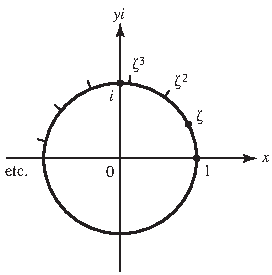
\includegraphics[width=0.373\linewidth,height=.8\textheight,keepaspectratio]{assets/p074_00.pdf}\end{center}
\begin{center}\small\textbf{5.27 Figure}\end{center}
\end{BookFloat}

\BookExerciseTitle{5}

\BookTextHeading{\textbf{Computations}}

\noindent In Exercises 1 through 6, determine whether the given subset of the complex numbers is a subgroup of the group \BookInline{\mathbb{C}} of complex numbers under addition.

\BookExercise{1.}{\BookInline{\mathbb{R}}}

\BookExercise{2.}{\BookInline{\mathbb{Q}^{+ }}}

\BookExercise{3.}{\BookInline{7\mathbb{Z}}}

\BookExercise{4.}{The set \BookInline{i\mathbb{R}} of pure imaginary numbers including 0}

\BookExercise{5.}{The set \BookInline{\pi \mathbb{Q}} of rational multiples of \BookInline{\pi }}

\BookExercise{6.}{The set \BookInline{\{\pi ^{n}\mid n\in \mathbb{Z}\}}}

\BookExercise{7.}{Which of the sets in Exercises 1 through 6 are subgroups of the group \BookInline{\mathbb{C}^{\ast }} of nonzero complex numbers under multiplication?}

\noindent In Exercises 8 through 13, determine whether the given set of invertible \BookInline{n\times n} matrices with real number entries is a subgroup of\textit{ GL}\BookInline{(n,\allowbreak \mathbb{R}).}

\BookExercise{8.}{The \BookInline{n\times n} matrices with determinant greater than or equal to 1}

\BookExercise{9.}{The diagonal \BookInline{n\times n} matrices with no zeros on the diagonal}

\BookExercise{10.}{The \BookInline{n\times n} matrices with determinant \BookInline{2^{k}} for some integer \BookInline{k}}

\BookExercise{11.}{The \BookInline{n\times n} matrices with determinant \BookInline{- 1}}

\BookExercise{12.}{The \BookInline{n\times n} matrices with determinant \BookInline{- 1} or 1}

\BookExercise{13.}{The set of all \BookInline{n\times n} matrices \BookInline{A} such that \BookInline{(A^{T})A= I_{n}.[}These matrices are called\textbf{ orthogonal.} Recall that \BookInline{A^{T},\allowbreak } the\textit{ transpose} of \BookInline{A,\allowbreak } is the matrix whose \BookInline{j}th column is the \BookInline{j}th row of \BookInline{A} for \BookInline{1\leq j\leq n,\allowbreak } and that the transpose operation has the property \BookInline{(AB)^{T}= (B^{T})(A^{T}).]}}

\noindent Let \BookInline{F} be the set of all real-valued functions with domain \BookInline{\mathbb{R}} and let \BookInline{\tilde { F }} be the subset of \BookInline{F} consisting of those functions that have a nonzero value at every point in \BookInline{\mathbb{R}.} In Exercises 14 through 19, determine whether the given subset of \BookInline{F} with the induced operation is (a) a subgroup of the group \BookInline{F} under addition, (b) a subgroup of the group \BookInline{\tilde { F }} under multiplication.

\BookExercise{14.}{The subset \BookInline{\tilde { F }}}

\BookExercise{15.}{The subset of all \BookInline{f\in F} such that \BookInline{f(1)= 0}}

\BookExercise{16.}{The subset of all \BookInline{f \in \tilde { F }} such that \BookInline{f(1)= 1}}

\BookExercise{17.}{The subset of all \BookInline{f \in \tilde { F }} such that \BookInline{f(0)= 1}}

\BookExercise{18.}{The subset of all \BookInline{f \in \tilde { F }} such that \BookInline{f(0)= - 1}}

\BookExercise{19.}{The subset of all constant functions in \BookInline{F.}}

\end{BookBody}

% Source PDF page 75; original printed page 58
\BookSource{75}{58}
\BookNarrativefalse

\begin{BookBody}

\BookExercise{20.}{Nine groups are given below. Give a\textit{ complete} list of all subgroup relations, of the form \BookInline{G_{i}\leq G_{j},\allowbreak } that exist between these given groups \BookInline{G_{1},\allowbreak G_{2},\allowbreak \cdots,\allowbreak G_{9}.} \BookInline{G_{1}= \mathbb{Z}} under addition \BookInline{G_{2}= 12\mathbb{Z}} under addition \BookInline{G_{3}= \mathbb{Q}^{+ }} under multiplication \BookInline{G_{4}= \mathbb{R}} under addition \BookInline{G_{5}= \mathbb{R}^{+ }} under multiplication \BookInline{G_{6}= \{\pi ^{n}\mid n\in \mathbb{Z}\}} under multiplication \BookInline{G_{7}= 3\mathbb{Z}} under addition \BookInline{G_{8}= } the set of all integral multiples of 6 under addition \BookInline{G_{9}= \{6^{n}\mid n\in \mathbb{Z}\}} under multiplication}

\BookExercise{21.}{Write at least 5 elements of each of the following cyclic groups. \textbf{a}\BookInline{.25\mathbb{Z}} under addition \textbf{b}\BookInline{.\{(\frac{1}{2})^{n}\mid n\in \mathbb{Z}\}} under multiplication \textbf{c}\BookInline{.\{\pi ^{n}\mid n\in \mathbb{Z}\}} under multiplication \textbf{d}\BookInline{.\langle \rho ^{3}\rangle } in the group \BookInline{D_{18}} \textbf{e}\BookInline{.\langle (1,\allowbreak 2,\allowbreak 3)(5,\allowbreak 6)\rangle } in the group \BookInline{S_{6}}}

\noindent In Exercises 22 through 25, describe all the elements in the cyclic subgroup of\textit{ GL}\BookInline{(2,\allowbreak \mathbb{R})} generated by the given \BookInline{2\times 2} \BookInline{\Big[\Big]} matrix. \BookInline{\Big[\Big]} \BookInline{\Big[\Big]} \BookInline{\Big[\Big]}

\BookExercise{22.}{\BookInline{\begin{bmatrix} 0 & - 1 \\ - 1 & 0 \end{bmatrix}}}

\BookExercise{23.}{\BookInline{\begin{bmatrix} 1 & 1 \\ 0 & 1 \end{bmatrix}}}

\BookExercise{24.}{\BookInline{\begin{bmatrix} 3 & 0 \\ 0 & 2 \end{bmatrix}}}

\BookExercise{25.}{\BookInline{\begin{bmatrix} 0 & - 2 \\ - 2 & 0 \end{bmatrix}}}

\BookExercise{26.}{Which of the following groups are cyclic? For each cyclic group, list all the generators of the group.}

\begin{center}\begin{adjustbox}{max width=\linewidth}\BookInline{\displaystyle G_{1}= \langle \mathbb{Z},\allowbreak + \rangle G_{2}= \langle \mathbb{Q},\allowbreak + \rangle G_{3}= \langle \mathbb{Q}^{+ },\allowbreak \cdot \rangle G_{4}= \langle 6\mathbb{Z},\allowbreak + \rangle}\end{adjustbox}\end{center}

\BookInline{G_{5}= \{6^{n}\mid n\in \mathbb{Z}\}} under multiplication

\BookInline{G_{6}= \{a+ b\sqrt{2}\mid a,\allowbreak b\in \mathbb{Z}\}} under addition

\noindent In Exercises 27 through 35, find the order of the cyclic subgroup of the given group generated by the indicated element.

\BookExercise{27.}{The subgroup of \BookInline{\mathbb{Z}_{4}} generated by 3}

\BookExercise{28.}{The subgroup of \BookInline{V} generated by \BookInline{c(}see Table 5.9)}

\BookExercise{29.}{The subgroup of \BookInline{U_{6}} generated by cos \BookInline{\begin{array} { r } { \frac { 2 \pi } { 3 } + i \sin \frac { 2 \pi } { 3 } } \end{array}}}

\BookExercise{30.}{The subgroup of \BookInline{\mathbb{Z}_{10}} generated by 8}

\BookExercise{31.}{The subgroup of \BookInline{\mathbb{Z}_{16}} generated by 12}

\BookExercise{32.}{The subgroup of the symmetric group \BookInline{S_{8}} generated by (2, 4, 6, 9)(3, 5, 7)}

\BookExercise{33.}{The subgroup of the symmetric group \BookInline{S_{10}} generated by (1, 10)(2, 9)(3, 8)(4, 7)(5, 6)}

\BookExercise{34.}{The subgroup of the multiplicative group \BookInline{G} of invertible \BookInline{4\times 4} matrices generated by}

\begin{center}\begin{adjustbox}{max width=\linewidth}\BookInline{\displaystyle \begin{bmatrix} 0 & 0 & 0 & 1 \\ 0 & 0 & 1 & 0 \\ 1 & 0 & 0 & 0 \\ 0 & 1 & 0 & 0 \end{bmatrix}}\end{adjustbox}\end{center}

\BookExercise{35.}{The subgroup of the multiplicative group \BookInline{G} of invertible \BookInline{4\times 4} matrices generated by}

\begin{center}\begin{adjustbox}{max width=\linewidth}\BookInline{\displaystyle \begin{bmatrix} 0 & 1 & 0 & 0 \\ 0 & 0 & 0 & 1 \\ 0 & 0 & 1 & 0 \\ 1 & 0 & 0 & 0 \end{bmatrix}}\end{adjustbox}\end{center}

\BookExercise{36.}{\textbf{. a} Complete Table 5.28 to give the group \BookInline{\mathbb{Z}_{6}} of 6 elements.}

\BookExercise{b.}{Compute the subgroups \BookInline{\langle 0\rangle,\allowbreak \langle 1\rangle,\allowbreak \langle 2\rangle,\allowbreak \langle 3\rangle,\allowbreak \langle 4\rangle,\allowbreak } and \BookInline{\langle 5\rangle } of the group \BookInline{\mathbb{Z}_{6}} given in part (a).}

\end{BookBody}

% Source PDF page 76; original printed page 59
\BookSource{76}{59}
\BookNarrativefalse

\begin{BookBody}

\BookExercise{c.}{Which elements are generators for the group \BookInline{\mathbb{Z}_{6}} of part (a)?}

\BookExercise{d.}{Give the subgroup diagram for the part (b) subgroups of \BookInline{\mathbb{Z}_{6}.(}We will see later that these are all the subgroups of \BookInline{\mathbb{Z}_{6}.)}}

\begin{BookFloat}{05_subgroups-p76-2}
\begin{center}\small\textbf{5.28 Table}\end{center}
\begin{center}\begin{adjustbox}{max width=\linewidth}
\renewcommand{\arraystretch}{1.2}\setlength{\tabcolsep}{5pt}
\begin{tabular}{c|c|c|c|c|c|c}
\BookInline{\mathbb{Z}_{6}:+ } & 0 & 1 & 2 & 3 & 4 & 5\\\hline
0 & 0 & 1 & 2 & 3 & 4 & 5\\\hline
1 & 1 & 2 & 3 & 4 & 5 & 0\\\hline
2 & 2 &  &  &  &  & \\\hline
3 & 3 &  &  &  &  & \\\hline
4 & 4 &  &  &  &  & \\\hline
5 & 5 &  &  &  &  & \\
\end{tabular}
\end{adjustbox}\end{center}
\end{BookFloat}

\BookTextHeading{\textbf{Concepts}}

\noindent In Exercises 37 and 38, correct the definition of the italicized term without reference to the text, if correction is needed, so that it is in a form acceptable for publication.

\BookExercise{37.}{A\textit{ subgroup} of a group \BookInline{G} is a subset \BookInline{H} of \BookInline{G} that contains the identity element \BookInline{e} of \BookInline{G} and also contains the inverse of each of its elements.}

\BookExercise{38.}{A group \BookInline{G} is\textit{ cyclic} if and only if there exists \BookInline{a\in G} such that \BookInline{G= \{a^{n}\mid n\in \mathbb{Z}\}.}}

\BookExercise{39.}{Determine whether each of the following is true or false.}

\BookExercise{a.}{The associative law holds in every group.}

\BookExercise{b.}{There may be a group in which the cancellation law fails.}

\BookExercise{c.}{Every group is a subgroup of itself.}

\BookExercise{d.}{Every group has exactly two improper subgroups.}

\BookExercise{e.}{In every cyclic group, every element is a generator.}

\BookExercise{f.}{A cyclic group has a unique generator.}

\BookExercise{g.}{Every set of numbers that is a group under addition is also a group under multiplication.}

\BookExercise{h.}{A subgroup may be defined as a subset of a group.}

\BookExercise{i.}{\textbf{i}\BookInline{.\mathbb{Z}_{4}} is a cyclic group.}

\BookExercise{j.}{Every subset of every group is a subgroup under the induced operation.}

\BookExercise{k.}{For any \BookInline{n\geq 3,\allowbreak } the dihedral group \BookInline{D_{n}} has at least \BookInline{n+ 2} cyclic subgroups.}

\BookExercise{40.}{Show by means of an example that it is possible for the quadratic equation \BookInline{x^{2}= e} to have more than two solutions in some group \BookInline{G} with identity \BookInline{e.}}

\noindent In Exercises 41 through 44 let \BookInline{B} be a subset of \BookInline{A,\allowbreak } and let \BookInline{b} be a particular element of \BookInline{B.} Determine whether the given set is a subgroup of the symmetric group \BookInline{S_{A}} under the induced operation. Here \BookInline{\sigma [B]= \{\sigma (x)\mid x\in B\}.}

\BookExercise{41.}{\BookInline{\{\sigma \in S_{A}\mid \sigma (b)= b\}}}

\BookExercise{42.}{\BookInline{\{\sigma \in S_{A}\mid \sigma (b)\in B\}}}

\BookExercise{43.}{\BookInline{\{\sigma \in S_{A}\mid \sigma [B]\subseteq B\}}}

\BookExercise{44.}{\BookInline{\{\sigma \in S_{A}\mid \sigma [B]= B\}}}

\BookTextHeading{\textbf{Theory}}

\noindent In Exercises 45 and 46, let \BookInline{\phi:G\to G^{\prime }} be an isomorphism of a group \BookInline{\langle G,\allowbreak \ast \rangle } with a group \BookInline{\langle G^{\prime },\allowbreak \ast ^{\prime }\rangle.} Write out a proof to convince a skeptic of the intuitively clear statement.

\end{BookBody}

% Source PDF page 77; original printed page 60
\BookSource{77}{60}
\BookNarrativefalse

\begin{BookBody}

\BookExercise{45.}{If \BookInline{H} is a subgroup of \BookInline{G,\allowbreak } then \BookInline{\phi [H]= \{\phi (h)\mid h\in H\}} is a subgroup of \BookInline{G^{\prime }.} That is, an isomorphism carries subgroups into subgroups.}

\BookExercise{46.}{If there is an \BookInline{a\in G} such that \BookInline{\langle a\rangle = G,\allowbreak } then \BookInline{G^{\prime }} is cyclic.}

\BookExercise{47.}{Show that if \BookInline{H} and \BookInline{K} are subgroups of an abelian group \BookInline{G,\allowbreak } then}

\begin{center}\begin{adjustbox}{max width=\linewidth}\BookInline{\displaystyle \{hk\mid h\in H\;\text{and}\;k\in K\}}\end{adjustbox}\end{center}

is a subgroup of \BookInline{G.}

\BookExercise{48.}{Find an example of a group \BookInline{G} and two subgroups \BookInline{H} and \BookInline{K} such that the set in Exercise 47 is not a subgroup of \BookInline{G.}}

\BookExercise{49.}{Prove that for any integer \BookInline{n\geq 3,\allowbreak S_{n}} has a subgroup isomorphic with \BookInline{D_{n}.}}

\BookExercise{50.}{Find the flaw in the following argument: “Condition 2 of Theorem 5.12 is redundant, since it can be derived from 1 and 3, for let \BookInline{a\in H.} Then \BookInline{a^{- 1}\in H} by 3, and by \BookInline{1,\allowbreak aa^{- 1}= e} is an element of \BookInline{H,\allowbreak } proving 2.”}

\BookExercise{51.}{Prove Theorem 5.15.}

\BookExercise{52.}{Prove that if \BookInline{G} is a cyclic group and \BookInline{|G|\geq 3,\allowbreak } then \BookInline{G} has at least 2 generators.}

\BookExercise{53.}{Prove that if \BookInline{G} is an abelian group, written multiplicatively, with identity element \BookInline{e,\allowbreak } then all elements \BookInline{x} of \BookInline{G} satisfying the equation \BookInline{x^{2}= e} form a subgroup \BookInline{H} of \BookInline{G.}}

\BookExercise{54.}{Repeat Exercise 53 for the general situation of the set \BookInline{H} of all solutions \BookInline{x} of the equation \BookInline{x^{n}= e} for a fixed integer \BookInline{n\geq 1} in an abelian group \BookInline{G} with identity \BookInline{e.}}

\BookExercise{55.}{Find a counterexample to Exercise 53 if the assumption of abelian is dropped.}

\BookExercise{56.}{Show that if \BookInline{a\in G,\allowbreak } where \BookInline{G} is a finite group with identity \BookInline{e,\allowbreak } then there exists \BookInline{n\in \mathbb{Z}^{+ }} such that \BookInline{a^{n}= e.}}

\BookExercise{57.}{Prove Theorem 5.16.}

\BookExercise{58.}{Let \BookInline{G} be a group and let \BookInline{a} be one fixed element of \BookInline{G.} Show that}

\begin{center}\begin{adjustbox}{max width=\linewidth}\BookInline{\displaystyle H_{a}= \{x\in G\mid xa= ax\}}\end{adjustbox}\end{center}

is a subgroup of \BookInline{G.}

\BookExercise{59.}{Generalizing Exercise 58, let \BookInline{S} be any subset of a group \BookInline{G.}}

\BookExercise{a.}{Show that \BookInline{H_{S}= \{x\in G\mid xs= sx} for all \BookInline{s\in S\}} is a subgroup of \BookInline{G.}}

\BookExercise{b.}{In reference to part (a), the subgroup \BookInline{H_{G}} is the\textbf{ center of} \BookInline{G.} Show that \BookInline{H_{G}} is an abelian group.}

\BookExercise{60.}{Let \BookInline{H} be a subgroup of a group \BookInline{G.} For \BookInline{a,\allowbreak b\in G,\allowbreak } let \BookInline{a\sim b} if and only if \BookInline{ab^{- 1}\in H.} Show that \BookInline{\sim } is an equivalence relation on \BookInline{G.}}

\BookExercise{61.}{For sets \BookInline{H} and \BookInline{K,\allowbreak } we define the\textbf{ intersection} \BookInline{H\cap K} by}

\begin{center}\begin{adjustbox}{max width=\linewidth}\BookInline{\displaystyle H\cap K= \{x\mid x\in H\;\text{and}\;x\in K\}.}\end{adjustbox}\end{center}

Show that if \BookInline{H\leq G} and \BookInline{K\leq G,\allowbreak } then \BookInline{H\cap K\leq G.(}Remember\BookInline{:\leq } denotes “is a subgroup of,” not “is a subset of.”)

\BookExercise{62.}{Prove that every cyclic group is abelian.}

\BookExercise{63.}{Let \BookInline{G} be a group and let \BookInline{G_{n}= \{g^{n}\mid g\in G\}.} Under what hypothesis about \BookInline{G} can we show that \BookInline{G_{n}} is a subgroup of \BookInline{G}?}

\BookExercise{64.}{Show that a group with no proper nontrivial subgroups is cyclic.}

\BookExercise{65.}{Cracker Barrel Restaurants place a puzzle called “Jump All But One Game” at each table. The puzzle starts with golf tees arranged in a triangle as in Figure 5.29a where the presence of a tee is noted with a solid dot and the absence is noted with a hollow dot. A move can be made if a tee can jump over one adjacent tee and land on an empty space. When a move is made, the tee that is jumped over is removed. A possible first move is shown in Figure 5.29b. The goal is to have just one remaining tee. Use the Klein 4-group to show that no matter what sequence of (legal) moves you make, the last remaining tee cannot be in a bottom corner position.}

\end{BookBody}

% Continuation on source PDF page 78, preceding Section 6
\BookNarrativetrue

\begin{BookBody}

\begin{BookFloat}{05_subgroups-p78-0}
\begin{center}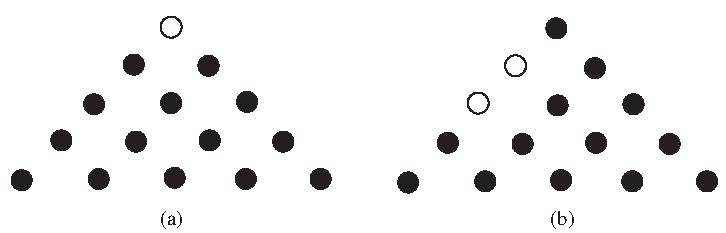
\includegraphics[width=0.995\linewidth,height=.8\textheight,keepaspectratio]{assets/p078_00.pdf}\end{center}
\begin{center}\small\textbf{5.29 Figure}\end{center}
\end{BookFloat}

\end{BookBody}
\ifdefined\BookMaster\let\BookFinish\relax\else\def\BookFinish{\end{document}}\fi\BookFinish

\clearpage
% !TeX program = xelatex
\ifdefined\BookMaster\else
\documentclass[11pt,oneside]{article}
% !TeX program = xelatex
\usepackage[b5paper,left=22mm,right=22mm,top=20mm,bottom=22mm,footskip=11mm]{geometry}
\usepackage{fontspec}
\setmainfont{TeX Gyre Termes}
\setsansfont{TeX Gyre Heros}
\usepackage{amsmath,amssymb,mathtools,amsthm}
\renewcommand{\cdots}{\mathinner{\cdotp\cdotp\cdotp}}
\usepackage{graphicx,adjustbox,array,booktabs,longtable,multirow,enumitem,changepage,needspace}
\usepackage[table]{xcolor}
\usepackage{fancyhdr}
\raggedbottom
\interfootnotelinepenalty=10000
\newcommand{\BookFootnote}[2]{\begingroup\renewcommand{\thefootnote}{\fnsymbol{footnote}}\footnote[#1]{#2}\endgroup}
\newcommand{\BookFootnoteMark}[1]{\begingroup\renewcommand{\thefootnote}{\fnsymbol{footnote}}\footnotemark[#1]\endgroup}
\newcommand{\BookFootnoteText}[2]{\begingroup\renewcommand{\thefootnote}{\fnsymbol{footnote}}\footnotetext[#1]{#2}\endgroup}
\newenvironment{BookFloat}[1]{\par\addvspace{.6\baselineskip}\noindent\def\BookFloatID{#1}\begin{minipage}{\linewidth}\phantomsection\label{bookfloat:#1:start}}{\phantomsection\label{bookfloat:\BookFloatID:end}\end{minipage}\par\addvspace{.6\baselineskip}}

\usepackage[unicode,hidelinks]{hyperref}
\pagestyle{fancy}
\fancyhf{}
\newcommand{\BookFooter}{}
\fancyfoot[L]{\parbox[b]{\dimexpr\textwidth-15mm}{\footnotesize\BookFooter}}
\fancyfoot[R]{\footnotesize\thepage}
\renewcommand{\headrulewidth}{0pt}
\renewcommand{\footrulewidth}{0pt}
\setlength{\parindent}{0pt}
\setlength{\parskip}{0.2em}
\setlength{\emergencystretch}{3em}
\setlist{nosep,leftmargin=1.7em,labelsep=.65em}
\newif\ifBookNarrative
\BookNarrativetrue
\newenvironment{BookBody}{\setlength{\parindent}{0pt}}{}
\newcommand{\BookStatement}[1]{\par\addvspace{.6\baselineskip}\noindent #1\enspace\ignorespaces}
\newcommand{\BookLabel}[1]{\par\addvspace{.6\baselineskip}\needspace{3\baselineskip}\noindent\textbf{#1}\quad\ignorespaces}
\newcommand{\BookHeading}[1]{\par\addvspace{\baselineskip}\needspace{4\baselineskip}\noindent{\large\bfseries #1}\par\medskip}
\newcommand{\BookSubheading}[1]{\par\addvspace{.7\baselineskip}\needspace{3\baselineskip}\noindent{\bfseries #1}\par\smallskip}
\newcommand{\BookTextHeading}[1]{\par\addvspace{.7\baselineskip}\needspace{3\baselineskip}\noindent #1\par\smallskip}
\newcommand{\BookSectionTitle}[2]{\par\addvspace{1.2\baselineskip}\needspace{5\baselineskip}\noindent\colorbox{gray!25}{\sffamily\bfseries\small SECTION #1}\quad{\large\bfseries #2}\par\medskip}
\newcommand{\BookExerciseTitle}[1]{\par\addvspace{\baselineskip}\needspace{4\baselineskip}\noindent{\color{gray}\rule{1.5mm}{1.5mm}}\enspace{\large\bfseries Exercises #1}\par\medskip}
\newcommand{\BookBullet}[1]{\begin{list}{\textbullet}{\setlength{\leftmargin}{1.7em}\setlength{\labelwidth}{1em}\setlength{\labelsep}{.7em}\setlength{\topsep}{0pt}\setlength{\parsep}{0pt}\setlength{\itemsep}{0pt}}\item #1\end{list}}
\newcommand{\BookExercise}[2]{\begin{list}{\textbf{#1}}{\setlength{\leftmargin}{2.2em}\setlength{\labelwidth}{1.5em}\setlength{\labelsep}{.7em}\setlength{\topsep}{.15em}\setlength{\parsep}{0pt}\setlength{\itemsep}{0pt}}\item #2\end{list}}
\newcommand{\BookEnd}[1]{\unskip\nobreak\hfill\ensuremath{#1}}
\newcommand{\BookSource}[2]{\phantomsection\label{sourcepage:#1}} % Source-page anchors, retained through reflow.
\usepackage{multicol}
\usepackage{tikz}
\newcommand{\BookPartEntry}[2]{\par\noindent\makebox[17mm][l]{\bfseries Section #1}#2\par}
\newcommand{\BookPartTitle}[3]{\par\bigskip\noindent\begin{tikzpicture}\node[anchor=north west,inner sep=0pt,outer sep=0pt] (bookpart) at (0,0) {\begin{minipage}{\dimexpr\linewidth-.5pt}\hspace*{26mm}\begin{minipage}[t]{\dimexpr\linewidth-26mm}\begin{adjustbox}{max width=\linewidth}{\fontsize{20}{24}\selectfont\bfseries #2}\end{adjustbox}\par\vspace{6mm}\hrule\vspace{6mm}{\sffamily\footnotesize\setlength{\parskip}{.3em}#3}\vspace{3mm}\end{minipage}\end{minipage}};\path[shade,top color=gray!60,bottom color=white] (0,0) rectangle ([xshift=24mm]bookpart.south west);\node[anchor=north,font=\sffamily\bfseries\small] at (12mm,-2mm) {PART};\node[anchor=north,font=\sffamily\bfseries\Huge] at (12mm,-7mm) {#1};\end{tikzpicture}\par\bigskip}
\newsavebox{\BookMathBox}
\makeatletter
\newcommand{\BookInline}[1]{\leavevmode\hskip0pt\relax\begingroup\in@{\begin}{#1}\ifin@\sbox{\BookMathBox}{\(#1\)}\ifdim\wd\BookMathBox>\dimexpr\linewidth-1em\relax\resizebox{\dimexpr\linewidth-1em\relax}{!}{\usebox{\BookMathBox}}\else\(#1\)\fi\else\in@{\left}{#1}\ifin@\sbox{\BookMathBox}{\(#1\)}\ifdim\wd\BookMathBox>\dimexpr\linewidth-1em\relax\resizebox{\dimexpr\linewidth-1em\relax}{!}{\usebox{\BookMathBox}}\else\(#1\)\fi\else\(#1\)\fi\fi\endgroup\hskip0pt\relax}
\makeatother
\DeclareMathOperator{\Aut}{Aut}
\DeclareMathOperator{\End}{End}
\DeclareMathOperator{\Hom}{Hom}
\DeclareMathOperator{\GF}{GF}
\DeclareMathOperator{\irr}{irr}
\DeclareMathOperator{\lt}{lt}
\DeclareMathOperator{\lp}{lp}
\providecommand{\textcircled}[1]{\textnormal{(#1)}}

\begin{document}
\fi
\renewcommand{\BookFooter}{Section 6 Cyclic Groups}
\pdfbookmark[0]{Section 6 Cyclic Groups}{06_cyclic_groups}
\ifdefined\BookMaster\else\setcounter{page}{61}\fi
% Source PDF page 78; original printed page 61
\BookSource{78}{61}
\BookNarrativetrue

\begin{BookBody}

\BookSectionTitle{6}{Cyclic Groups}

\noindent Recall the following facts and notations from Section 5. If \BookInline{G} is a group and \BookInline{a\in G,\allowbreak } then

\begin{center}\begin{adjustbox}{max width=\linewidth}\BookInline{\displaystyle H= \{a^{n}\mid n\in \mathbb{Z}\}}\end{adjustbox}\end{center}

\noindent is a subgroup of \BookInline{G(}Theorem 5.19). This group is the\textbf{ cyclic subgroup} \BookInline{\langle a\rangle } \textbf{of} \BookInline{G} \textbf{gener}\textbf{ated by} \BookInline{a.} Also, given a group \BookInline{G} and an element \BookInline{a} in \BookInline{G,\allowbreak } if

\begin{center}\begin{adjustbox}{max width=\linewidth}\BookInline{\displaystyle G= \{a^{n}\mid n\in \mathbb{Z}\},\allowbreak }\end{adjustbox}\end{center}

\noindent then \BookInline{a} is a\textbf{ generator of} \BookInline{G} and the group \BookInline{G= \langle a\rangle } is\textbf{ cyclic.} We introduce one new bit of terminology. Let \BookInline{a} be an element of a group \BookInline{G.} If the cyclic subgroup \BookInline{\langle a\rangle } of \BookInline{G} is finite, then the\textbf{ order of} \BookInline{a} is the order \BookInline{|\langle a\rangle |} of this cyclic subgroup. Otherwise, we say that \BookInline{a} is of\textbf{ infinite order.} We will see in this section that if \BookInline{a\in G} is of finite order \BookInline{m,\allowbreak } then \BookInline{m} is the smallest positive integer such that \BookInline{a^{m}= e.}

The first goal of this section is to describe all cyclic groups and all subgroups of cyclic groups. This is not an idle exercise. We will see later that cyclic groups serve as building blocks for a significant class of abelian groups, in particular, for all finite abelian groups. Cyclic groups are fundamental to the understanding of groups.

\BookTextHeading{\textbf{Elementary Properties of Cyclic Groups}  }

\noindent We start with a demonstration that cyclic groups are abelian.

\BookLabel{6.1 Theorem} Every cyclic group is abelian.

\BookLabel{\textit{Proof}} Let \BookInline{G} be a cyclic group and let \BookInline{a} be a generator of \BookInline{G} so that

\begin{center}\begin{adjustbox}{max width=\linewidth}\BookInline{\displaystyle G= \langle a\rangle = \{a^{n}\mid n\in \mathbb{Z}\}.}\end{adjustbox}\end{center}

\noindent If \BookInline{g_{1}} and \BookInline{g_{2}} are any two elements of \BookInline{G,\allowbreak } there exist integers \BookInline{r} and \BookInline{s} such that \BookInline{g_{1}= a^{r}} and \BookInline{g_{2}= a^{s}.} Then

\begin{center}\begin{adjustbox}{max width=\linewidth}\BookInline{\displaystyle g_{1}g_{2}= a^{r}a^{s}= a^{r+ s}= a^{s+ r}= a^{s}a^{r}= g_{2}g_{1},\allowbreak }\end{adjustbox}\end{center}

\noindent so \BookInline{G} is abelian. \BookEnd{\blacklozenge}

We shall continue to use multiplicative notation for our general work on cyclic groups, even though they are abelian.

The\textit{ division algorithm} that follows is well known and seems pretty simple. In fact, this algorithm is taught in elementary school. If you divide an integer \BookInline{n} by a positive integer \BookInline{m,\allowbreak } you get an integer quotient \BookInline{q} with a remainder \BookInline{r} where \BookInline{0\leq r<m.} You might write this as \BookInline{n\div m= q} R \BookInline{r,\allowbreak } which of course means \BookInline{\begin{array} { r } { \frac { n } { m } = q + \frac { r } { m } } \end{array}}. Multiplying both sides by \BookInline{m} gives the form of the division algorithm that is a fundamental tool for the study of cyclic groups.

\end{BookBody}

% Source PDF page 79; original printed page 62
\BookSource{79}{62}
\BookNarrativetrue

\begin{BookBody}

\BookExercise{6.}{\textbf{6.2 Division Algorithm for} \BookInline{\mathbb{Z}} If \BookInline{m} is a positive integer and \BookInline{n} is any integer, then there exist unique integers \BookInline{q} and \BookInline{r} such that}

\begin{center}\begin{adjustbox}{max width=\linewidth}\BookInline{\displaystyle n= mq+ r\;\text{and}\;0\leq r<m.}\end{adjustbox}\end{center}

\BookLabel{\textit{Proof}} We give an intuitive diagrammatic explanation, using Fig. 6.3. On the number line, mark off the multiples of \BookInline{m} and the position of \BookInline{n.} Now \BookInline{n} falls either on a multiple \BookInline{qm} of \BookInline{m} and \BookInline{r} can be taken as 0, or \BookInline{n} falls between two multiples of \BookInline{m.} If the latter is the case, let \BookInline{qm} be the first multiple of \BookInline{m} to the left of \BookInline{n.} Then \BookInline{r} is as shown in Fig. 6.3. Note that \BookInline{0\leq r<m.} Uniqueness of \BookInline{q} and \BookInline{r} follows since if \BookInline{n} is not a multiple of \BookInline{m} so that we can take \BookInline{r= 0,\allowbreak } then there is a unique multiple \BookInline{qm} of \BookInline{m} to the left of \BookInline{n} and at distance less than \BookInline{m} from \BookInline{n,\allowbreak } as illustrated in Fig\BookInline{.6.3.}\BookEnd{\blacklozenge}

\begin{BookFloat}{06_cyclic_groups-p79-3}
\begin{center}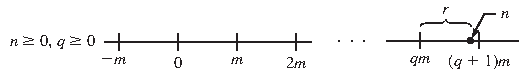
\includegraphics[width=0.717\linewidth,height=.8\textheight,keepaspectratio]{assets/p079_07.pdf}\end{center}
\end{BookFloat}

\begin{BookFloat}{06_cyclic_groups-p79-4}
\begin{center}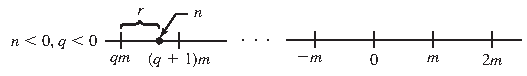
\includegraphics[width=0.723\linewidth,height=.8\textheight,keepaspectratio]{assets/p079_08.pdf}\end{center}
\begin{center}\small\textbf{6.3 Figure}\end{center}
\end{BookFloat}

In the notation of the division algorithm, we regard \BookInline{q} as the\textbf{ quotient} and \BookInline{r} as the nonnegative\textbf{ remainder} when \BookInline{n} is divided by \BookInline{m.}

\BookLabel{6.4 Example} Find the quotient \BookInline{q} and remainder \BookInline{r} when 38 is divided by 7 according to the division algorithm.

\BookLabel{\textit{Solution}} The positive multiples of 7 are \BookInline{7,\allowbreak 14,\allowbreak 21,\allowbreak 28,\allowbreak 35,\allowbreak 42,\allowbreak \cdots.} Choosing the multiple to leave a nonnegative remainder less than 7, we write

\begin{center}\begin{adjustbox}{max width=\linewidth}\BookInline{\displaystyle 38= 35+ 3= 7(5)+ 3}\end{adjustbox}\end{center}

\noindent so the quotient is \BookInline{q= 5} and the remainder is \BookInline{r= 3.} \BookEnd{\blacktriangle}

\BookLabel{6.5 Example} Find the quotient \BookInline{q} and remainder \BookInline{r} when \BookInline{- 38} is divided by 7 according to the division algorithm.

\BookLabel{\textit{Solution}} The negative multiples of 7 are \BookInline{- 7,\allowbreak - 14,\allowbreak - 21,\allowbreak - 28,\allowbreak - 35,\allowbreak - 42,\allowbreak \cdots.} Choosing the multiple to leave a nonnegative remainder less than 7, we write

\begin{center}\begin{adjustbox}{max width=\linewidth}\BookInline{\displaystyle - 38= - 42+ 4= 7(- 6)+ 4}\end{adjustbox}\end{center}

\noindent so the quotient is \BookInline{q= - 6} and the remainder is \BookInline{r= 4.} \BookEnd{\blacktriangle}

We will use the division algorithm to show that a subgroup \BookInline{H} of a cyclic group \BookInline{G} is also cyclic. Think for a moment what we will have to do to prove this. We will have to use the\textit{ definition} of a cyclic group since we have proved little about cyclic groups yet. That is, we will have to use the fact that \BookInline{G} has a generating element \BookInline{a.} We must then exhibit, in terms of this generator \BookInline{a,\allowbreak } some generator \BookInline{c= a^{m}} for \BookInline{H} in order to show that \BookInline{H} is cyclic. There is really only one natural choice for the power \BookInline{m} of \BookInline{a} to try. Can you guess what it is before you read the proof of the theorem?

\end{BookBody}

% Source PDF page 80; original printed page 63
\BookSource{80}{63}
\BookNarrativetrue

\begin{BookBody}

\BookLabel{6.6 Theorem} A subgroup of a cyclic group is cyclic.

\BookLabel{\textit{Proof}} Let \BookInline{G} be a cyclic group generated by \BookInline{a} and let \BookInline{H} be a subgroup of \BookInline{G.} If \BookInline{H= \{e\},\allowbreak } then \BookInline{H= \langle e\rangle } is cyclic. If \BookInline{H\neq \{e\},\allowbreak } then \BookInline{a^{n}\in H} for some \BookInline{n\in \mathbb{Z}^{+ }.} Let \BookInline{m} be the smallest integer in \BookInline{\mathbb{Z}^{+ }} such that \BookInline{a^{m}\in H.}

We claim that \BookInline{c= a^{m}} generates \BookInline{H;} that is,

\begin{center}\begin{adjustbox}{max width=\linewidth}\BookInline{\displaystyle H= \langle a^{m}\rangle = \langle c\rangle .}\end{adjustbox}\end{center}

\noindent We must show that every \BookInline{b\in H} is a power of \BookInline{c.} Since \BookInline{b\in H} and \BookInline{H\leq G,\allowbreak } we have \BookInline{b= a^{n}} for some \BookInline{n.} Find \BookInline{q} and \BookInline{r} such that

\begin{center}\begin{adjustbox}{max width=\linewidth}\BookInline{\displaystyle n= mq+ r\;\text{for}\;0\leq r<m}\end{adjustbox}\end{center}

\noindent in accord with the division algorithm. Then

\begin{center}\begin{adjustbox}{max width=\linewidth}\BookInline{\displaystyle a^{n}= a^{mq+ r}= (a^{m})^{q}a^{r},\allowbreak }\end{adjustbox}\end{center}

\noindent so

\begin{center}\begin{adjustbox}{max width=\linewidth}\BookInline{\displaystyle a^{r}= (a^{m})^{- q}a^{n}.}\end{adjustbox}\end{center}

\noindent Now since \BookInline{a^{n}\in H,\allowbreak a^{m}\in H,\allowbreak } and \BookInline{H} is a group, both \BookInline{(a^{m})^{- q}} and \BookInline{a^{n}} are in \BookInline{H.} Thus

\begin{center}\begin{adjustbox}{max width=\linewidth}\BookInline{\displaystyle (a^{m})^{- q}a^{n}\in H;\;\text{that is}\;,\allowbreak a^{r}\in H.}\end{adjustbox}\end{center}

\noindent Since \BookInline{m} was the smallest positive integer such that \BookInline{a^{m}\in H} and \BookInline{0\leq r<m,\allowbreak } we must have \BookInline{r= 0.} Thus \BookInline{n= mq} and

\begin{center}\begin{adjustbox}{max width=\linewidth}\BookInline{\displaystyle b= a^{n}= (a^{m})^{q}= c^{q},\allowbreak }\end{adjustbox}\end{center}

\noindent so \BookInline{b} is a power of \BookInline{c.} \BookEnd{\blacklozenge}

As noted in Examples 5.24 and \BookInline{5.25,\allowbreak \mathbb{Z}} under addition is cyclic and for a positive integer \BookInline{n,\allowbreak } the set \BookInline{n\mathbb{Z}} of all multiples of \BookInline{n} is a subgroup of \BookInline{\mathbb{Z}} under addition, the cyclic subgroup generated by \BookInline{n.} Theorem 6.6 shows that these cyclic subgroups are the only subgroups of \BookInline{\mathbb{Z}} under addition. We state this as a corollary.

\BookLabel{6.7 Corollary} The subgroups of \BookInline{\mathbb{Z}} under addition are precisely the groups \BookInline{n\mathbb{Z}} under addition for \BookInline{n\in \mathbb{Z}.} \BookEnd{\blacklozenge}

This corollary gives us an elegant way to define the\textit{ greatest common divisor} of two positive integers \BookInline{r} and \BookInline{s.} Exercise 54 shows that \BookInline{H= \{nr+ ms\mid n,\allowbreak m\in \mathbb{Z}\}} is a subgroup of the group \BookInline{\mathbb{Z}} under addition. Thus \BookInline{H} must be cyclic and have a generator \BookInline{d,\allowbreak } which we may choose to be positive.

\BookLabel{6.8 Definition} Let \BookInline{r} be a positive integer and \BookInline{s} be a non-negative integer. The positive generator \BookInline{d} of the cyclic group

\begin{center}\begin{adjustbox}{max width=\linewidth}\BookInline{\displaystyle H= \{nr+ ms\mid n,\allowbreak m\in \mathbb{Z}\}}\end{adjustbox}\end{center}

\noindent under addition is the\textbf{ greatest common divisor} (abbreviated gcd) of \BookInline{r} and \BookInline{s.} We write \BookInline{d= } gcd\BookInline{(r,\allowbreak s).}\BookEnd{\blacksquare}

Note that \BookInline{d\mathbb{Z}= H,\allowbreak r= 1r+ 0s\in H,\allowbreak } and \BookInline{s= 0r+ 1s\in H.} This implies that \BookInline{r,\allowbreak s\in } \BookInline{d\mathbb{Z},\allowbreak } which says that \BookInline{d} is a divisor of both \BookInline{r} and \BookInline{s.} Since \BookInline{d\in H,\allowbreak } we can write

\begin{center}\begin{adjustbox}{max width=\linewidth}\BookInline{\displaystyle d= nr+ ms}\end{adjustbox}\end{center}

\noindent for some integers \BookInline{n} and \BookInline{m.} We see that every integer dividing both \BookInline{r} and \BookInline{s} divides the right-hand side of the equation, and hence must be a divisor of \BookInline{d} also. Thus \BookInline{d} must 
% Source PDF page 81; original printed page 64
\BookSource{81}{64}
be the largest number dividing both \BookInline{r} and \BookInline{s;} this accounts for the name given to \BookInline{d} in Definition 6.8.

\end{BookBody}

\BookNarrativetrue

\begin{BookBody}

The fact that the greatest common divisor \BookInline{d} of \BookInline{r} and \BookInline{s} can be written in the form \BookInline{d= nr+ ms} for some integers \BookInline{n} and \BookInline{m} is called Be´zout’s identity. Be´zout’s identity is very useful in number theory, as we will see in studying cyclic groups.

\BookLabel{6.9 Example} Find the gcd of 42 and 72.

\BookLabel{\textit{Solution}} The positive divisors of 42 are 1, 2, 3, 6, 7, 14, 21, and 42. The positive divisors of 72 are 1, 2, 3, 4, 6, 8, 9, 12, 18, 24, 36, and 72. The greatest common divisor is 6. Note that \BookInline{6= (3)(72)+ (- 5)(42).} There is an algorithm for expressing the greatest common divisor \BookInline{d} of \BookInline{r} and \BookInline{s} in the form \BookInline{d= nr+ ms,\allowbreak } but we will not need to make use of it here. The interested reader can find the algorithm by searching the Internet for the Euclidean algorithm and Be´zout’s identity\BookInline{.}\BookEnd{\blacktriangle}

Two positive integers are\textbf{ relatively prime} if their gcd is 1. For example, 12 and 25 are relatively prime. Note that they have no prime factors in common. In our discussion of subgroups of cyclic groups, we will need to know the following:

If \BookInline{r} and \BookInline{s} are relatively prime and if \BookInline{r} divides \BookInline{sm,\allowbreak } then \BookInline{r} must divide \BookInline{m.(1)}

\noindent Let’s prove this. If \BookInline{r} and \BookInline{s} are relatively prime, then we may write

\begin{center}\begin{adjustbox}{max width=\linewidth}\BookInline{\displaystyle 1= ar+ bs\;\text{for some}\;a,\allowbreak b\in \mathbb{Z}.}\end{adjustbox}\end{center}

\noindent Multiplying by \BookInline{m,\allowbreak } we obtain

\begin{center}\begin{adjustbox}{max width=\linewidth}\BookInline{\displaystyle m= arm+ bsm.}\end{adjustbox}\end{center}

\noindent Now \BookInline{r} divides both \BookInline{arm} and \BookInline{bsm} since \BookInline{r} divides \BookInline{sm.} Thus \BookInline{r} is a divisor of the right-hand side of this equation, so \BookInline{r} must divide \BookInline{m.}

\BookTextHeading{\textbf{The Structure of Cyclic Groups}  }

\noindent We can now describe all cyclic groups, up to an isomorphism.

\BookLabel{6.10 Theorem} Let \BookInline{G} be a cyclic group with generator \BookInline{a.} If the order of \BookInline{G} is infinite, then \BookInline{G} is isomorphic to \BookInline{\langle \mathbb{Z},\allowbreak + \rangle.} If \BookInline{G} has finite order \BookInline{n,\allowbreak } then \BookInline{G} is isomorphic to \BookInline{\langle \mathbb{Z}_{n},\allowbreak + _{n}\rangle.}

\BookLabel{\textit{Proof}} \textbf{Case I} \textit{For all positive integers} \BookInline{m,\allowbreak } \BookInline{a ^ { m } \neq e.} In this case we claim that no two distinct exponents \BookInline{h} and \BookInline{k} can give equal elements \BookInline{a^{h}} and \BookInline{a^{k}} of \BookInline{G.} Suppose that \BookInline{a^{h}= a^{k}} and say \BookInline{h>k.} Then

\begin{center}\begin{adjustbox}{max width=\linewidth}\BookInline{\displaystyle a^{h}a^{- k}= a^{h- k}= e,\allowbreak }\end{adjustbox}\end{center}

contrary to our Case I assumption. Hence every element of \BookInline{G} can be expressed as \BookInline{a^{m}} for a unique \BookInline{m\in \mathbb{Z}.} The map \BookInline{\phi:G\to \mathbb{Z}} given by \BookInline{\phi (a^{i})= i} is thus well defined, one-to-one, and onto \BookInline{\mathbb{Z}.} Also,

\begin{center}\begin{adjustbox}{max width=\linewidth}\BookInline{\displaystyle \phi (a^{i}a^{j})= \phi (a^{i+ j})= i+ j= \phi (a^{i})+ \phi (a^{j}),\allowbreak }\end{adjustbox}\end{center}

so the homomorphism property is satisfied and \BookInline{\phi } is an isomorphism.

\end{BookBody}

% Source PDF page 82; original printed page 65
\BookSource{82}{65}
\BookNarrativetrue

\begin{BookBody}

\textbf{Case II} \BookInline{a^{m}= e} \textit{for some positive integer} \BookInline{m.} Let \BookInline{n} be the smallest positive integer such that \BookInline{a^{n}= e.} If \BookInline{s\in \mathbb{Z}} and \BookInline{s= nq+ r} for \BookInline{0\leq r<n,\allowbreak } then \BookInline{a^{s}= a^{nq+ r}= (a^{n})^{q}a^{r}= e^{q}a^{r}= a^{r}.} As in Case 1, if \BookInline{0\leq k<h<n} and \BookInline{a^{h}= a^{k},\allowbreak } then \BookInline{a^{h- k}= e} and \BookInline{0<h- k<n,\allowbreak } contradicting our choice of \BookInline{n.} Thus the elements

\begin{center}\begin{adjustbox}{max width=\linewidth}\BookInline{\displaystyle a^{0}= e,\allowbreak a,\allowbreak a^{2},\allowbreak a^{3},\allowbreak \cdots ,\allowbreak a^{n- 1}}\end{adjustbox}\end{center}

are all distinct and comprise all elements of \BookInline{G.} The map \BookInline{\psi:G\to \mathbb{Z}_{n}} given by \BookInline{\psi (a^{i})= i} for \BookInline{i= 0,\allowbreak 1,\allowbreak 2,\allowbreak \cdots,\allowbreak n- 1} is thus well defined, one-to-one, and onto \BookInline{\mathbb{Z}_{n}.} Because \BookInline{a^{n}= e,\allowbreak } we see that \BookInline{a^{i}a^{j}= a^{k}} where \BookInline{k= i+ _{n}j.} Thus

\begin{center}\begin{adjustbox}{max width=\linewidth}\BookInline{\displaystyle \psi (a^{i}a^{j})= i+ _{n}j= \psi (a^{i})+ _{n}\psi (a^{j}),\allowbreak }\end{adjustbox}\end{center}

so the homomorphism property is satisfied and \BookInline{\psi } is an isomorphism. \BookEnd{\blacklozenge}

\begin{BookFloat}{06_cyclic_groups-p82-6}
\begin{center}
\begin{minipage}[t]{0.4820\linewidth}\vspace{0pt}\begin{center}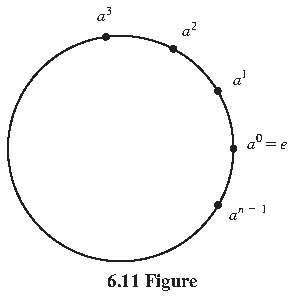
\includegraphics[width=\linewidth,height=.8\textheight,keepaspectratio]{assets/p082_06.pdf}\end{center}\end{minipage}\hfill\begin{minipage}[t]{0.4565\linewidth}\vspace{0pt}\begin{center}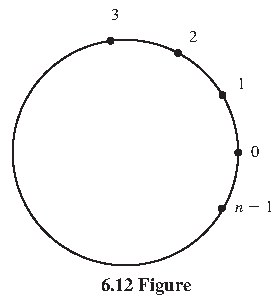
\includegraphics[width=\linewidth,height=.8\textheight,keepaspectratio]{assets/p082_07.pdf}\end{center}\end{minipage}
\end{center}
\end{BookFloat}

\BookLabel{6.13 Example} Motivated by our work with \BookInline{U_{n},\allowbreak } it is nice to visualize the elements \BookInline{e= a^{0},\allowbreak a^{1},\allowbreak a^{2},\allowbreak \cdots,\allowbreak } \BookInline{a^{n- 1}} of a cyclic group of order \BookInline{n} as being distributed evenly on a circle (see Fig. 6.11). The element \BookInline{a^{h}} is located \BookInline{h} of these equal units counterclockwise along the circle, measured from the right where \BookInline{e= a^{0}} is located. To multiply \BookInline{a^{h}} and \BookInline{a^{k}} diagrammatically, we start from \BookInline{a^{h}} and go \BookInline{k} additional units around counterclockwise. To see arithmetically where we end up, find \BookInline{q} and \BookInline{r} such that

\begin{center}\begin{adjustbox}{max width=\linewidth}\BookInline{\displaystyle h+ k= nq+ r\;\text{for}\;0\leq r<n.}\end{adjustbox}\end{center}

\noindent The \BookInline{nq} takes us all the way around the circle \BookInline{q} times, and we then wind up at \BookInline{a^{r}.}\BookEnd{\blacktriangle}

Figure 6.12 is essentially the same as Fig. 6.11 but with the points labeled with the exponents on the generator. The operation on these exponents is\textit{ addition modulo} \BookInline{n.}

This is simply the isomorphism between \BookInline{\langle a\rangle } and \BookInline{\mathbb{Z}_{n}.} Of course this is the same isomorphism we saw when we defined \BookInline{\mathbb{Z}_{n}} from \BookInline{U_{n},\allowbreak } but using \BookInline{a} instead of \BookInline{\zeta.}

As promised at the beginning of this section, we can see now that the order of an element \BookInline{a} in a group \BookInline{G} is simply the smallest positive number \BookInline{n} such that \BookInline{a^{n}= e.}

\BookLabel{6.14 Example} Let us find the order of the \BookInline{k-}cycle\BookInline{,\allowbreak \sigma = (a_{1},\allowbreak a_{2},\allowbreak a_{3},\allowbreak...,\allowbreak a_{k}),\allowbreak } in the symmetric group. The order of \BookInline{\sigma } is the smallest postive power of \BookInline{\sigma } that is \BookInline{\iota.} Note that applying \BookInline{\sigma } just maps each number to the next one in the cyclic order. So after \BookInline{k} applications of \BookInline{\sigma,\allowbreak } each number maps back to itself, but not before \BookInline{k} applications of \BookInline{\sigma.} Therefore, the order of a \BookInline{k-}cycle is \BookInline{k.}\BookEnd{\blacktriangle}

\end{BookBody}

% Source PDF page 83; original printed page 66
\BookSource{83}{66}
\BookNarrativetrue

\begin{BookBody}

\BookTextHeading{\textbf{Subgroups of Finite Cyclic Groups}  }

\noindent We have completed our description of cyclic groups and turn to their subgroups. Corollary 6.7 gives us complete information about subgroups of infinite cyclic groups. Let us give the basic theorem regarding generators of subgroups for the finite cyclic groups.

\BookLabel{6.15 Theorem} Let \BookInline{G} be a cyclic group with \BookInline{n} elements and generated by \BookInline{a.} Let \BookInline{b\in G} and let \BookInline{b= a^{s}.} Then \BookInline{b} generates a cyclic subgroup \BookInline{H} of \BookInline{G} containing \BookInline{n/d} elements, where \BookInline{d} is the greatest common divisor of \BookInline{n} and \BookInline{s.} Also\BookInline{,\allowbreak \langle a^{s}\rangle = \langle a^{t}\rangle } if and only if gcd\BookInline{(s,\allowbreak n)= } gcd\BookInline{(t,\allowbreak n).}

\BookLabel{\textit{Proof}} That \BookInline{b} generates a cyclic subgroup \BookInline{H} of \BookInline{G} is known from Theorem 5.19. We need show only that \BookInline{H} has \BookInline{n/d} elements. Following the argument of Case II of Theorem 6.10, we see that \BookInline{H} has as many elements as the smallest positive power \BookInline{m} of \BookInline{b} that gives the identity. Now \BookInline{b= a^{s},\allowbreak } and \BookInline{b^{m}= e} if and only if \BookInline{(a^{s})^{m}= e,\allowbreak } or if and only if \BookInline{n} divides \BookInline{ms.} What is the smallest positive integer \BookInline{m} such that \BookInline{n} divides \BookInline{ms}? Let \BookInline{d} be the gcd of \BookInline{n} and \BookInline{s.} Then there exist integers \BookInline{u} and \BookInline{v} such that

\begin{center}\begin{adjustbox}{max width=\linewidth}\BookInline{\displaystyle d= un+ vs.}\end{adjustbox}\end{center}

\noindent Since \BookInline{d} divides both \BookInline{n} and \BookInline{s,\allowbreak } we may write

\begin{center}\begin{adjustbox}{max width=\linewidth}\BookInline{\displaystyle 1= u(n/d)+ v(s/d)}\end{adjustbox}\end{center}

\noindent where both \BookInline{n/d} and \BookInline{s/d} are integers. This last equation shows that \BookInline{n/d} and \BookInline{s/d} are relatively prime, for any integer dividing both of them must also divide 1. We wish to find the smallest positive \BookInline{m} such that

\begin{center}\begin{adjustbox}{max width=\linewidth}\BookInline{\displaystyle { \frac { m s } { n } } = { \frac { m ( s / d ) } { ( n / d ) } } { \mathrm { ~ i s ~ a n ~ i n t e g e r } } .}\end{adjustbox}\end{center}

\noindent From the division property (1) following Example 6.9, we conclude that \BookInline{n/d} must divide \BookInline{m,\allowbreak } so the smallest such \BookInline{m} is \BookInline{n/d.} Thus the order of \BookInline{H} is \BookInline{n/d.}

Taking for the moment \BookInline{\mathbb{Z}_{n}} as a model for a cyclic group of order \BookInline{n,\allowbreak } we see that if \BookInline{d} is a divisor of \BookInline{n,\allowbreak } then the cyclic subgroup \BookInline{\langle d\rangle } of \BookInline{\mathbb{Z}_{n}} has \BookInline{n/d} elements, and contains all the positive integers \BookInline{m} less than \BookInline{n} such that gcd\BookInline{(m,\allowbreak n)= d.} Thus there is only one subgroup of \BookInline{\mathbb{Z}_{n}} of order \BookInline{n/d.} Taken with the preceding paragraph, this shows at once that if \BookInline{a} is a generator of the cyclic group \BookInline{G,\allowbreak } then \BookInline{\langle a^{s}\rangle = \langle a^{t}\rangle } if and only if gcd\BookInline{(s,\allowbreak n)= } gcd\BookInline{(t,\allowbreak n).}\BookEnd{\blacklozenge}

\BookLabel{6.16 Example} For an example using additive notation, consider \BookInline{\mathbb{Z}_{12},\allowbreak } with the generator \BookInline{a= 1.} Since the greatest common divisor of 3 and 12 is \BookInline{3,\allowbreak 3= 3\cdot 1} generates a subgroup of \BookInline{\textstyle { \frac { 1 2 } { 3 } } = 4} elements, namely

\begin{center}\begin{adjustbox}{max width=\linewidth}\BookInline{\displaystyle \langle 3\rangle = \{0,\allowbreak 3,\allowbreak 6,\allowbreak 9\}.}\end{adjustbox}\end{center}

\noindent Since the gcd of 8 and 12 is 4, 8 generates a subgroup of \BookInline{\textstyle { \frac { 1 2 } { 4 } } = 3} elements, namely,

\begin{center}\begin{adjustbox}{max width=\linewidth}\BookInline{\displaystyle \langle 8\rangle = \{0,\allowbreak 4,\allowbreak 8\}.}\end{adjustbox}\end{center}

\noindent Since the gcd of 12 and 5 is 1, 5 generates a subgroup of \BookInline{\textstyle { \frac { 1 2 } { 1 } } = 1 2} elements; that is, 5 is a generator of the whole group \BookInline{\mathbb{Z}_{12}.}\BookEnd{\blacktriangle}

The following corollary follows immediately from Theorem 6.15.

\BookLabel{6.17 Corollary} If \BookInline{a} is a generator of a finite cyclic group \BookInline{G} of order \BookInline{n,\allowbreak } then the other generators of \BookInline{G} are the elements of the form \BookInline{a^{r},\allowbreak } where \BookInline{r} is relatively prime to \BookInline{n.}

\end{BookBody}

% Source PDF page 84; original printed page 67
\BookSource{84}{67}
\BookNarrativetrue

\begin{BookBody}

\BookLabel{6.18 Example} Let us find all subgroups of \BookInline{\mathbb{Z}_{18}} and give their subgroup diagram. All subgroups are cyclic. By Corollary 6.17, the elements 1, 5, 7, 11, 13, and 17 are all generators of \BookInline{\mathbb{Z}_{18}.} Starting with 2,

\begin{center}\begin{adjustbox}{max width=\linewidth}\BookInline{\displaystyle \langle 2\rangle = \{0,\allowbreak 2,\allowbreak 4,\allowbreak 6,\allowbreak 8,\allowbreak 10,\allowbreak 12,\allowbreak 14,\allowbreak 16\}.}\end{adjustbox}\end{center}

\noindent is of order 9 and has as generators elements of the form \BookInline{h2,\allowbreak } where \BookInline{h} is relatively prime to 9, namely\BookInline{,\allowbreak h= 1,\allowbreak 2,\allowbreak 4,\allowbreak 5,\allowbreak 7,\allowbreak } and 8, so \BookInline{h2= 2,\allowbreak 4,\allowbreak 8,\allowbreak 10,\allowbreak 14,\allowbreak } and 16. The element 6 of \BookInline{\langle 2\rangle } generates \BookInline{\{0,\allowbreak 6,\allowbreak 12\},\allowbreak } and 12 also is a generator of this subgroup.

We have thus far found all subgroups generated by 0, 1, 2, 4, 5, 6, 7, 8, 10, 11, 12, 13, 14, 16, and 17. This leaves just 3, 9, and 15 to consider.

\begin{center}\begin{adjustbox}{max width=\linewidth}\BookInline{\displaystyle \langle 3\rangle = \{0,\allowbreak 3,\allowbreak 6,\allowbreak 9,\allowbreak 12,\allowbreak 15\},\allowbreak }\end{adjustbox}\end{center}

\noindent and 15 also generates this group of order 6, since \BookInline{15= 5\cdot 3,\allowbreak } and the gcd of 5 and 6 is 1. Finally,

\begin{center}\begin{adjustbox}{max width=\linewidth}\BookInline{\displaystyle \langle 9\rangle = \{0,\allowbreak 9\}.}\end{adjustbox}\end{center}

\noindent The subgroup diagram for these subgroups of \BookInline{\mathbb{Z}_{18}} is given in Fig. 6.19.

\begin{BookFloat}{06_cyclic_groups-p84-8}
\begin{center}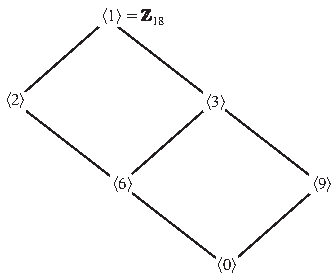
\includegraphics[width=0.459\linewidth,height=.8\textheight,keepaspectratio]{assets/p084_10.pdf}\end{center}
\begin{center}\small\textbf{6.19 Figure}\end{center}
\end{BookFloat}

Subgroup diagram for \BookInline{\mathbb{Z}_{18}.}

This example is straightforward; we are afraid we wrote it out in such detail that it may look complicated. The exercises give some practice along these lines\BookInline{.}\BookEnd{\blacktriangle}

\BookLabel{6.20 Corollary} Let \BookInline{G} be a finite cyclic group and \BookInline{H\leq G.} Then \BookInline{|H|} divides \BookInline{|G|.} That is\BookInline{,\allowbreak |G|} is a multiple of \BookInline{|H|.}

\BookLabel{\textit{Proof}} Let \BookInline{g} be a generator for \BookInline{G} and let \BookInline{n= |G|.} By Theorem \BookInline{6.6,\allowbreak H} is cyclic, so there is an element in \BookInline{h\in H} such that \BookInline{h} generates \BookInline{H.} Since \BookInline{h\in H\leq G,\allowbreak h= g^{s}} for some \BookInline{s.} Theorem 6.15 states that

\begin{center}\begin{adjustbox}{max width=\linewidth}\BookInline{\displaystyle | H | = { \frac { n } { \operatorname* { g c d } ( n ,\allowbreak  s ) } }}\end{adjustbox}\end{center}

\noindent which is a divisor of \BookInline{n.} \BookEnd{\blacklozenge}

\BookLabel{6.21 Example} We find all orders of the subgroups of \BookInline{\mathbb{Z}_{28}.} Factoring gives \BookInline{28= 2^{2}\cdot 7,\allowbreak } so the possible orders of subgroups of the cyclic group \BookInline{\mathbb{Z}_{28}} are 1, 2, 4, 7, 14, and 28. We note that \BookInline{|\langle 0\rangle |= 1,\allowbreak |\langle 14\rangle |= 2,\allowbreak |\langle 7\rangle |= 4,\allowbreak |\langle 4\rangle |= 7,\allowbreak |\langle 2\rangle |= 14,\allowbreak |\langle 1\rangle |= |\mathbb{Z}_{28}|= 28.} So there are subgroups of order 1, 2, 4, 7, 14, and \BookInline{28.}\BookEnd{\blacktriangle}

Actually, Corollary 6.20 can be strengthened considerably. The assumption that \BookInline{G} is cyclic is completely unnecessary. As we will see in Section 10, Lagrange’s Theorem states that for any finite group, the order of a subgroup divides the order of the group.

\end{BookBody}

% Source PDF page 85; original printed page 68
\BookSource{85}{68}
\BookNarrativefalse

\begin{BookBody}

\BookExerciseTitle{6}

\BookTextHeading{\textbf{Computations}}

\noindent In Exercises 1 through 4, find the quotient and remainder, according to the division algorithm, when \BookInline{n} is divided by \BookInline{m.}

\BookExercise{1.}{\BookInline{n= 42,\allowbreak m= 9}}

\BookExercise{2.}{\BookInline{n= - 42,\allowbreak m= 9}}

\BookExercise{3.}{\BookInline{n= - 37,\allowbreak m= 8}}

\BookExercise{4.}{\BookInline{n= 37,\allowbreak m= 8}}

\noindent In Exercises 5 through 7, find the greatest common divisor of the two integers.

\BookExercise{5.}{32 and 24}

\BookExercise{6.}{48 and 88}

\BookExercise{7.}{360 and 420}

\noindent In Exercises 8 through 11, find the number of generators of a cyclic group having the given order.

\BookExercise{8.}{5}

\BookExercise{9.}{8}

\BookExercise{10.}{24}

\BookExercise{11.}{84}

\noindent An isomorphism of a group with itself is an\textbf{ automorphism of the group.} In Exercises 12 through 16, find the number of automorphisms of the given group. [\textit{Hint:} You may use Exercise 53. What must be the image of a generator under an automorphism?]

\BookExercise{12.}{\BookInline{\mathbb{Z}_{2}}}

\BookExercise{13.}{\BookInline{\mathbb{Z}_{6}}}

\BookExercise{14.}{\BookInline{\mathbb{Z}_{8}}}

\BookExercise{15.}{\BookInline{\mathbb{Z}}}

\BookExercise{16.}{\BookInline{\mathbb{Z}_{84}}}

\noindent In Exercises 17 through 23, find the number of elements in the indicated cyclic group.

\BookExercise{17.}{The cyclic subgroup of \BookInline{\mathbb{Z}_{30}} generated by 25}

\BookExercise{18.}{The cyclic subgroup of \BookInline{\mathbb{Z}_{42}} generated by 30}

\BookExercise{19.}{The cyclic subgroup \BookInline{\langle i\rangle } of the group \BookInline{\mathbb{C}^{\ast }} of nonzero complex numbers under multiplication}

\BookExercise{20.}{The cyclic subgroup of the group \BookInline{\mathbb{C}^{\ast }} of Exercise 19 generated by \BookInline{(1+ i)/\sqrt{2}}}

\BookExercise{21.}{The cyclic subgroup of the group \BookInline{\mathbb{C}^{\ast }} of Exercise 19 generated by \BookInline{1+ i}}

\BookExercise{22.}{The cyclic subgroup \BookInline{\langle \rho ^{10}\rangle } of \BookInline{D_{24}}}

\BookExercise{23.}{The cyclic subgoup \BookInline{\langle \rho ^{35}\rangle } of \BookInline{D_{375}}}

\BookExercise{24.}{Consider the group \BookInline{S_{10}} \textbf{a.} What is the order of the cycle (2, 4, 6, 7)? \textbf{b.} What is the order of (1, 4)(2, 3, 5)? Of (1, 3)(2, 4, 6, 7, 8)? \textbf{c.} What is the order of (1, 5, 9)(2, 6, 7)? Of (1, 3)(2, 5, 6, 8)? \textbf{d.} What is the order of (1, 2)(3, 4, 5, 6, 7, 8)? Of (1, 2, 3)(4, 5, 6, 7, 8, 9)?}

\BookExercise{e.}{State a theorem suggested by parts (c) and (d). [Hint: The important words you are looking for are\textit{ least} \textit{common multiple}.]}

\noindent In Exercises 25 through 30, find the maximum possibe order for an element of \BookInline{S_{n}} for a given value of \BookInline{n.}

\BookExercise{25.}{\BookInline{n= 5}}

\BookExercise{26.}{\BookInline{n= 6}}

\BookExercise{27.}{\BookInline{n= 7}}

\BookExercise{28.}{\BookInline{n= 8}}

\BookExercise{29.}{\BookInline{n= 10}}

\BookExercise{30.}{\BookInline{n= 15}}

\noindent In Exercises 31 through 33, find all subgroups of the given group, and draw the subgroup diagram for the subgroups.

\BookExercise{31.}{\BookInline{\mathbb{Z}_{12}}}

\BookExercise{32.}{\BookInline{\mathbb{Z}_{36}}}

\BookExercise{33.}{\BookInline{\mathbb{Z}_{8}}}

\noindent In Exercises 34 through 38, find all orders of subgroups of the given group.

\BookExercise{34.}{\BookInline{\mathbb{Z}_{6}}}

\BookExercise{35.}{\BookInline{\mathbb{Z}_{8}}}

\BookExercise{36.}{\BookInline{\mathbb{Z}_{12}}}

\BookExercise{37.}{\BookInline{\mathbb{Z}_{20}}}

\BookExercise{38.}{\BookInline{\mathbb{Z}_{17}}}

\BookTextHeading{\textbf{Concepts}}

\noindent In Exercises 39 and 40, correct the definition of the italicized term without reference to the text, if correction is needed, so that it is in a form acceptable for publication.

\BookExercise{39.}{An element \BookInline{a} of a group \BookInline{G} has\textit{ order} \BookInline{n\in \mathbb{Z}^{+ }} if and only if \BookInline{a^{n}= e.}}

\BookExercise{40.}{The\textit{ greatest common divisor} of two positive integers is the largest positive integer that divides both of them.}

\end{BookBody}

% Source PDF page 86; original printed page 69
\BookSource{86}{69}
\BookNarrativefalse

\begin{BookBody}

\BookExercise{41.}{Determine whether each of the following is true or false.}

\BookExercise{a.}{Every cyclic group is abelian.}

\BookExercise{b.}{Every abelian group is cyclic.}

\BookExercise{c.}{\textbf{c}\BookInline{.\mathbb{Q}} under addition is a cyclic group.}

\BookExercise{d.}{Every element of every cyclic group generates the group.}

\BookExercise{e.}{There is at least one abelian group of every finite order \BookInline{>0.}}

\BookExercise{f.}{Every group of order \BookInline{\leq 4} is cyclic.}

\BookExercise{g.}{All generators of \BookInline{\mathbb{Z}_{20}} are prime numbers.}

\BookExercise{h.}{If \BookInline{G} and \BookInline{G^{\prime }} are groups, then \BookInline{G\cap G^{\prime }} is a group.}

\BookExercise{i.}{If \BookInline{H} and \BookInline{K} are subgroups of a group \BookInline{G,\allowbreak } then \BookInline{H\cap K} is a group.}

\BookExercise{j.}{Every cyclic group of order \BookInline{>2} has at least two distinct generators.}

\noindent In Exercises 42 through 46, either give an example of a group with the property described, or explain why no example exists.

\BookExercise{42.}{A finite abelian group that is not cyclic}

\BookExercise{43.}{An infinite group that is not cyclic}

\BookExercise{44.}{A cyclic group having only one generator}

\BookExercise{45.}{An infinite cyclic group having four generators}

\BookExercise{46.}{A finite cyclic group having four generators}

\noindent The generators of the cyclic multiplicative group \BookInline{U_{n}} of all \BookInline{n}th roots of unity in \BookInline{\mathbb{C}} are the\textbf{ primitive} \BookInline{n}th\textbf{ roots of} \textbf{unity}. In Exercises 47 through 50, find the primitive \BookInline{n}th roots of unity for the given value of \BookInline{n.}

\BookExercise{47.}{\BookInline{n= 4}}

\BookExercise{48.}{\BookInline{n= 6}}

\BookExercise{49.}{\BookInline{n= 8}}

\BookExercise{50.}{\BookInline{n= 12}}

\BookLabel{\textit{Proof}} \textbf{ Synopsis}

\BookExercise{51.}{Give a one-sentence synopsis of the proof of Theorem 6.1.}

\BookExercise{52.}{Give at most a three-sentence synopsis of the proof of Theorem 6.6.}

\BookTextHeading{\textbf{Theory}}

\BookExercise{53.}{Let \BookInline{G} be a cyclic group with generator \BookInline{a,\allowbreak } and let \BookInline{G^{\prime }} be a group isomorphic to \BookInline{G.} If \BookInline{\phi:G\to G^{\prime }} is an isomorphism, show that, for every \BookInline{x\in G,\allowbreak \phi (x)} is completely determined by the value \BookInline{\phi (a).} That is, if \BookInline{\phi:G\to G^{\prime }} and \BookInline{\psi:G\to G^{\prime }} are two isomophisms such that \BookInline{\phi (a)= \psi (a),\allowbreak } then \BookInline{\phi (x)= \psi (x)} for all \BookInline{x\in G.}}

\BookExercise{54.}{Let \BookInline{r} and \BookInline{s} be integers. Show that \BookInline{\{nr+ ms\mid n,\allowbreak m\in \mathbb{Z}\}} is a subgroup of \BookInline{\mathbb{Z}.}}

\BookExercise{55.}{Prove that if \BookInline{G} is a finite cyclic group\BookInline{,\allowbreak H} and \BookInline{K} are subgroups of \BookInline{G,\allowbreak } and \BookInline{H\neq K,\allowbreak } then \BookInline{|H|\neq |K|.}}

\BookExercise{56.}{Let \BookInline{a} and \BookInline{b} be elements of a group \BookInline{G.} Show that if \BookInline{ab} has finite order \BookInline{n,\allowbreak } then \BookInline{ba} also has order \BookInline{n.}}

\BookExercise{57.}{Let \BookInline{r} and \BookInline{s} be positive integers.}

\BookExercise{a.}{Define the\textbf{ least common multiple} of \BookInline{r} and \BookInline{s} as a generator of a certain cyclic group.}

\BookExercise{b.}{Under what condition is the least common multiple of \BookInline{r} and \BookInline{s} their product\BookInline{,\allowbreak rs}?}

\BookExercise{c.}{Generalizing part (b), show that the product of the greatest common divisor and of the least common multiple of \BookInline{r} and \BookInline{s} is \BookInline{rs.}}

\end{BookBody}

% Continuation on source PDF page 87, preceding Section 7
\BookNarrativefalse

\begin{BookBody}

\BookExercise{58.}{Show that a group that has only a finite number of subgroups must be a finite group.}

\BookExercise{59.}{Show by a counterexample that the following “converse” of Theorem 6.6 is not a theorem: “If a group \BookInline{G} is such that every proper subgroup is cyclic, then \BookInline{G} is cyclic.”}

\BookExercise{60.}{Let \BookInline{G} be a group and suppose \BookInline{a\in G} generates a cyclic subgroup of order 2 and is the\textit{ unique} such element. Show that\textit{ ax} \BookInline{= xa} for all \BookInline{x\in G.[}\textit{Hint:} Consider \BookInline{(xax^{- 1})^{2}.]}}

\BookExercise{61.}{Prove that if \BookInline{G} is a cyclic group with an odd number of generators, then \BookInline{G} has two elements.}

\BookExercise{62.}{Let \BookInline{p} and \BookInline{q} be distinct prime numbers. Find the number of generators of the cyclic group \BookInline{\mathbb{Z}_{pq}.}}

\BookExercise{63.}{Let \BookInline{p} be a prime number. Find the number of generators of the cyclic group \BookInline{\mathbb{Z}_{p}^{r},\allowbreak } where \BookInline{r} is an integer \BookInline{\geq 1.}}

\BookExercise{64.}{Show that in a finite cyclic group \BookInline{G} of order \BookInline{n,\allowbreak } written multiplicatively, the equation \BookInline{x^{m}= e} has exactly \BookInline{m} solutions \BookInline{x} in \BookInline{G} for each positive integer \BookInline{m} that divides \BookInline{n.}}

\BookExercise{65.}{With reference to Exercise 64, what is the situation if \BookInline{1<m<n} and \BookInline{m} does not divide \BookInline{n}?}

\BookExercise{66.}{Show that \BookInline{\mathbb{Z}_{p}} has no proper nontrivial subgroups if \BookInline{p} is a prime number.}

\BookExercise{67.}{Let \BookInline{G} be an abelian group and let \BookInline{H} and \BookInline{K} be finite cyclic subgroups with \BookInline{|H|= r} and \BookInline{|K|= s.}}

\BookExercise{a.}{Show that if \BookInline{r} and \BookInline{s} are relatively prime, then \BookInline{G} contains a cyclic subgroup of order \BookInline{rs.}}

\BookExercise{b.}{Generalizing part (a), show that \BookInline{G} contains a cyclic subgroup of order the least common multiple of \BookInline{r} and \BookInline{s.}}

\end{BookBody}
\ifdefined\BookMaster\let\BookFinish\relax\else\def\BookFinish{\end{document}}\fi\BookFinish

\clearpage
% !TeX program = xelatex
\ifdefined\BookMaster\else
\documentclass[11pt,oneside]{article}
% !TeX program = xelatex
\usepackage[b5paper,left=22mm,right=22mm,top=20mm,bottom=22mm,footskip=11mm]{geometry}
\usepackage{fontspec}
\setmainfont{TeX Gyre Termes}
\setsansfont{TeX Gyre Heros}
\usepackage{amsmath,amssymb,mathtools,amsthm}
\renewcommand{\cdots}{\mathinner{\cdotp\cdotp\cdotp}}
\usepackage{graphicx,adjustbox,array,booktabs,longtable,multirow,enumitem,changepage,needspace}
\usepackage[table]{xcolor}
\usepackage{fancyhdr}
\raggedbottom
\interfootnotelinepenalty=10000
\newcommand{\BookFootnote}[2]{\begingroup\renewcommand{\thefootnote}{\fnsymbol{footnote}}\footnote[#1]{#2}\endgroup}
\newcommand{\BookFootnoteMark}[1]{\begingroup\renewcommand{\thefootnote}{\fnsymbol{footnote}}\footnotemark[#1]\endgroup}
\newcommand{\BookFootnoteText}[2]{\begingroup\renewcommand{\thefootnote}{\fnsymbol{footnote}}\footnotetext[#1]{#2}\endgroup}
\newenvironment{BookFloat}[1]{\par\addvspace{.6\baselineskip}\noindent\def\BookFloatID{#1}\begin{minipage}{\linewidth}\phantomsection\label{bookfloat:#1:start}}{\phantomsection\label{bookfloat:\BookFloatID:end}\end{minipage}\par\addvspace{.6\baselineskip}}

\usepackage[unicode,hidelinks]{hyperref}
\pagestyle{fancy}
\fancyhf{}
\newcommand{\BookFooter}{}
\fancyfoot[L]{\parbox[b]{\dimexpr\textwidth-15mm}{\footnotesize\BookFooter}}
\fancyfoot[R]{\footnotesize\thepage}
\renewcommand{\headrulewidth}{0pt}
\renewcommand{\footrulewidth}{0pt}
\setlength{\parindent}{0pt}
\setlength{\parskip}{0.2em}
\setlength{\emergencystretch}{3em}
\setlist{nosep,leftmargin=1.7em,labelsep=.65em}
\newif\ifBookNarrative
\BookNarrativetrue
\newenvironment{BookBody}{\setlength{\parindent}{0pt}}{}
\newcommand{\BookStatement}[1]{\par\addvspace{.6\baselineskip}\noindent #1\enspace\ignorespaces}
\newcommand{\BookLabel}[1]{\par\addvspace{.6\baselineskip}\needspace{3\baselineskip}\noindent\textbf{#1}\quad\ignorespaces}
\newcommand{\BookHeading}[1]{\par\addvspace{\baselineskip}\needspace{4\baselineskip}\noindent{\large\bfseries #1}\par\medskip}
\newcommand{\BookSubheading}[1]{\par\addvspace{.7\baselineskip}\needspace{3\baselineskip}\noindent{\bfseries #1}\par\smallskip}
\newcommand{\BookTextHeading}[1]{\par\addvspace{.7\baselineskip}\needspace{3\baselineskip}\noindent #1\par\smallskip}
\newcommand{\BookSectionTitle}[2]{\par\addvspace{1.2\baselineskip}\needspace{5\baselineskip}\noindent\colorbox{gray!25}{\sffamily\bfseries\small SECTION #1}\quad{\large\bfseries #2}\par\medskip}
\newcommand{\BookExerciseTitle}[1]{\par\addvspace{\baselineskip}\needspace{4\baselineskip}\noindent{\color{gray}\rule{1.5mm}{1.5mm}}\enspace{\large\bfseries Exercises #1}\par\medskip}
\newcommand{\BookBullet}[1]{\begin{list}{\textbullet}{\setlength{\leftmargin}{1.7em}\setlength{\labelwidth}{1em}\setlength{\labelsep}{.7em}\setlength{\topsep}{0pt}\setlength{\parsep}{0pt}\setlength{\itemsep}{0pt}}\item #1\end{list}}
\newcommand{\BookExercise}[2]{\begin{list}{\textbf{#1}}{\setlength{\leftmargin}{2.2em}\setlength{\labelwidth}{1.5em}\setlength{\labelsep}{.7em}\setlength{\topsep}{.15em}\setlength{\parsep}{0pt}\setlength{\itemsep}{0pt}}\item #2\end{list}}
\newcommand{\BookEnd}[1]{\unskip\nobreak\hfill\ensuremath{#1}}
\newcommand{\BookSource}[2]{\phantomsection\label{sourcepage:#1}} % Source-page anchors, retained through reflow.
\usepackage{multicol}
\usepackage{tikz}
\newcommand{\BookPartEntry}[2]{\par\noindent\makebox[17mm][l]{\bfseries Section #1}#2\par}
\newcommand{\BookPartTitle}[3]{\par\bigskip\noindent\begin{tikzpicture}\node[anchor=north west,inner sep=0pt,outer sep=0pt] (bookpart) at (0,0) {\begin{minipage}{\dimexpr\linewidth-.5pt}\hspace*{26mm}\begin{minipage}[t]{\dimexpr\linewidth-26mm}\begin{adjustbox}{max width=\linewidth}{\fontsize{20}{24}\selectfont\bfseries #2}\end{adjustbox}\par\vspace{6mm}\hrule\vspace{6mm}{\sffamily\footnotesize\setlength{\parskip}{.3em}#3}\vspace{3mm}\end{minipage}\end{minipage}};\path[shade,top color=gray!60,bottom color=white] (0,0) rectangle ([xshift=24mm]bookpart.south west);\node[anchor=north,font=\sffamily\bfseries\small] at (12mm,-2mm) {PART};\node[anchor=north,font=\sffamily\bfseries\Huge] at (12mm,-7mm) {#1};\end{tikzpicture}\par\bigskip}
\newsavebox{\BookMathBox}
\makeatletter
\newcommand{\BookInline}[1]{\leavevmode\hskip0pt\relax\begingroup\in@{\begin}{#1}\ifin@\sbox{\BookMathBox}{\(#1\)}\ifdim\wd\BookMathBox>\dimexpr\linewidth-1em\relax\resizebox{\dimexpr\linewidth-1em\relax}{!}{\usebox{\BookMathBox}}\else\(#1\)\fi\else\in@{\left}{#1}\ifin@\sbox{\BookMathBox}{\(#1\)}\ifdim\wd\BookMathBox>\dimexpr\linewidth-1em\relax\resizebox{\dimexpr\linewidth-1em\relax}{!}{\usebox{\BookMathBox}}\else\(#1\)\fi\else\(#1\)\fi\fi\endgroup\hskip0pt\relax}
\makeatother
\DeclareMathOperator{\Aut}{Aut}
\DeclareMathOperator{\End}{End}
\DeclareMathOperator{\Hom}{Hom}
\DeclareMathOperator{\GF}{GF}
\DeclareMathOperator{\irr}{irr}
\DeclareMathOperator{\lt}{lt}
\DeclareMathOperator{\lp}{lp}
\providecommand{\textcircled}[1]{\textnormal{(#1)}}

\begin{document}
\fi
\renewcommand{\BookFooter}{Section 7 Generating Sets and Cayley Digraphs}
\pdfbookmark[0]{Section 7 Generating Sets and Cayley Digraphs}{07_generating_sets_and_cayley_digraphs}
\ifdefined\BookMaster\else\setcounter{page}{70}\fi
% Source PDF page 87; original printed page 70
\BookSource{87}{70}
\BookNarrativetrue

\begin{BookBody}

\BookSectionTitle{7}{Generating Sets and Cayley Digraphs}

\noindent Let \BookInline{G} be a group, and let \BookInline{a\in G.} We have described the cyclic subgroup \BookInline{\langle a\rangle } of \BookInline{G,\allowbreak } which is the smallest subgroup of \BookInline{G} that contains the element \BookInline{a.} Suppose we want to find as small a subgroup as possible that contains both \BookInline{a} and \BookInline{b} for another element \BookInline{b} in \BookInline{G.} By Theorem 5.19, we see that any subgroup containing \BookInline{a} and \BookInline{b} must contain \BookInline{a^{n}} and \BookInline{b^{m}} for all \BookInline{m,\allowbreak n\in \mathbb{Z},\allowbreak } and consequently must contain all finite products of such powers of \BookInline{a} and \BookInline{b.} For example, such an expression might be \BookInline{a^{2}b^{4}a^{- 3}b^{2}a^{5}.} Note that we cannot “simplify” this expression by writing first all powers of \BookInline{a} followed by the powers of \BookInline{b,\allowbreak } since \BookInline{G} may not be abelian. However, products of such expressions are again expressions of the same type. Furthermore\BookInline{,\allowbreak e= a^{0}} and the inverse of such an expression is again of the same type. For example, the inverse of \BookInline{a^{2}b^{4}a^{- 3}b^{2}a^{5}} is \BookInline{a^{- 5}b^{- 2}a^{3}b^{- 4}a^{- 2}.} By Theorem 5.12, this shows that all such products of integral powers of \BookInline{a} and \BookInline{b} form a subgroup of \BookInline{G,\allowbreak } which surely must be the smallest subgroup containing both \BookInline{a} and \BookInline{b.} We call \BookInline{a} and \BookInline{b} \textbf{generators} of this subgroup. If this subgroup should be all of \BookInline{G,\allowbreak } then we say that \BookInline{\{a,\allowbreak b\}} \textbf{generates} \BookInline{G.} Of course, there is nothing sacred about taking just two elements \BookInline{a,\allowbreak b\in G.} We could have made similar arguments for three, four, or any number of elements of \BookInline{G,\allowbreak } as long as we take only finite products of their integral powers.

\BookLabel{7.1 Example} As we have seen, the dihedral group is generated by \BookInline{\{\mu,\allowbreak \rho \}} since every element in \BookInline{D_{n}} can be written in the form \BookInline{\rho ^{k}} or \BookInline{\mu \rho ^{k}} for \BookInline{0\leq k<n.} Also\BookInline{,\allowbreak \{\mu,\allowbreak \mu \rho \}} generates \BookInline{D_{n}} since \BookInline{\rho = \mu (\mu \rho ),\allowbreak } so any element in the dihedral group can also be written as a product of copies of \BookInline{\mu } and \BookInline{\mu \rho.} It is interesting to note that both \BookInline{\mu } and \BookInline{\mu \rho } have order 2, while in the generating set \BookInline{\{\mu,\allowbreak \rho \}} one element has order 2, but the other has order \BookInline{n.}\BookEnd{\blacktriangle}

\BookLabel{7.2 Example} The Klein 4-group \BookInline{V= \{e,\allowbreak a,\allowbreak b,\allowbreak c\}} of Example 5.7 is generated by \BookInline{\{a,\allowbreak b\}} since \BookInline{ab= c.} It is also generated by \BookInline{\{a,\allowbreak c\},\allowbreak \{b,\allowbreak c\},\allowbreak } and \BookInline{\{a,\allowbreak b,\allowbreak c\}.} If a group \BookInline{G} is generated by a subset \BookInline{S,\allowbreak } then every subset of \BookInline{G} containing \BookInline{S} generates \BookInline{G.}\BookEnd{\blacktriangle}

\BookLabel{7.3 Example} The group \BookInline{\mathbb{Z}_{6}} is generated by \BookInline{\{1\}} and \BookInline{\{5\}.} It is also generated by \BookInline{\{2,\allowbreak 3\}} since \BookInline{2+ 3= 5,\allowbreak } so that any subgroup containing 2 and 3 must contain 5 and must therefore be \BookInline{\mathbb{Z}_{6}.} It is also generated by \BookInline{\{3,\allowbreak 4\},\allowbreak \{2,\allowbreak 3,\allowbreak 4\},\allowbreak \{1,\allowbreak 3\},\allowbreak } and \BookInline{\{3,\allowbreak 5\},\allowbreak } but it is not generated by \BookInline{\{2,\allowbreak 4\}} since \BookInline{\langle 2\rangle = \{0,\allowbreak 2,\allowbreak 4\}} contains 2 and \BookInline{4.}\BookEnd{\blacktriangle}

\end{BookBody}

% Source PDF page 88; original printed page 71
\BookSource{88}{71}
\BookNarrativetrue

\begin{BookBody}

We have given an intuitive explanation of the subgroup of a group \BookInline{G} generated by a subset of \BookInline{G.} What follows is a detailed exposition of the same idea approached in another way, namely via intersections of subgroups. After we get an intuitive grasp of a concept, it is nice to try to write it up as neatly as possible. We give a set-theoretic definition and generalize a theorem that was in Exercise 61 of Section 5.

\BookLabel{7.4 Definition} Let \BookInline{\{S_{i}\mid i\in I\}} be a collection of sets. Here \BookInline{I} may be any set of indices. The\textbf{ intersection} \BookInline{\cap _{i\in I}S_{i}} \textbf{of the sets} \BookInline{S_{i}} is the set of all elements that are in all the sets \BookInline{S_{i};} that is,

\begin{center}\begin{adjustbox}{max width=\linewidth}\BookInline{\displaystyle \bigcap _ { i \in I } S _ { i } = \{ x   |   x \in S _ { i } { \mathrm { ~ f o r ~ a l l ~ } } i \in I \} .}\end{adjustbox}\end{center}

\noindent If \BookInline{I} is finite\BookInline{,\allowbreak I= \{1,\allowbreak 2,\allowbreak...,\allowbreak n\},\allowbreak } we may denote \BookInline{\cap _{i\in I}S_{i}} by

\begin{center}\begin{adjustbox}{max width=\linewidth}\BookInline{\displaystyle S_{1}\cap S_{2}\cap \cdots \cap S_{n}.}\end{adjustbox}\end{center} \BookEnd{\blacksquare}

\BookLabel{7.5 Theorem} For any group \BookInline{G} and any nonempty collection of subgroups \BookInline{\{H_{i}\leq G\mid i\in I\},\allowbreak } the intersection of all the subgroups \BookInline{H_{i},\allowbreak \cap _{i\in I}H_{i},\allowbreak } is also a subgroup of \BookInline{G.}

\BookLabel{\textit{Proof}} Let us show closure. Let \BookInline{a\in \cap _{i\in I}H_{i}} and \BookInline{b\in \cap _{i\in I}H_{i},\allowbreak } so that \BookInline{a\in H_{i}} for all \BookInline{i\in I} and \BookInline{b\in H_{i}} for all \BookInline{i\in I.} Then \BookInline{ab\in H_{i}} for all \BookInline{i\in I,\allowbreak } since \BookInline{H_{i}} is a group. Thus \BookInline{ab\in \cap _{i\in I}H_{i}.} Since \BookInline{H_{i}} is a subgroup for all \BookInline{i\in I,\allowbreak } we have \BookInline{e\in H_{i}} for all \BookInline{i\in I,\allowbreak } and hence \BookInline{e\in \cap _{i\in I}H_{i}.}

Finally, for \BookInline{a\in \cap _{i\in I}H_{i},\allowbreak } we have \BookInline{a\in H_{i}} for all \BookInline{i\in I,\allowbreak } so \BookInline{a^{- 1}\in H_{i}} for all \BookInline{i\in I,\allowbreak } which implies that \BookInline{a^{- 1}\in \cap _{i\in I}H_{i}.}\BookEnd{\blacklozenge}

Let \BookInline{G} be a group and let \BookInline{a_{i}\in G} for \BookInline{i\in I.} There is at least one subgroup of \BookInline{G} containing all the elements \BookInline{a_{i}} for \BookInline{i\in I,\allowbreak } namely \BookInline{G} is itself. Theorem 7.5 assures us that if we take the intersection of all subgroups of \BookInline{G} containing all \BookInline{a_{i}} for \BookInline{i\in I,\allowbreak } we will obtain a subgroup \BookInline{H} of \BookInline{G.} This subgroup \BookInline{H} is the smallest subgroup of \BookInline{G} containing all the \BookInline{a_{i}} for \BookInline{i\in I.}

\BookLabel{7.6 Definition} Let \BookInline{G} be a group and let \BookInline{a_{i}\in G} for \BookInline{i\in I.} The smallest subgroup of \BookInline{G} containing \BookInline{\{a_{i}\mid i\in } \BookInline{I\}} is the\textbf{ subgroup generated by} \BookInline{\{a_{i}\mid i\in I\}.} If this subgroup is all of \BookInline{G,\allowbreak } then \BookInline{\{a_{i}\mid i\in } \BookInline{I\}} \textbf{generates} \BookInline{G} and the \BookInline{a_{i}} are\textbf{ generators of} \BookInline{G.} If there is a finite set \BookInline{\{a_{i}\mid i\in I\}} that generates \BookInline{G,\allowbreak } then \BookInline{G} is\textbf{ finitely generated}\BookInline{.}\BookEnd{\blacksquare}

Note that this definition is consistent with our previous definition of a generator for a cyclic group. Note also that the statement \BookInline{a} \textit{is} \BookInline{a} \textit{generator of} \BookInline{G} may mean either that \BookInline{G= \langle a\rangle } or that \BookInline{a} is a member of a subset of \BookInline{G} that generates \BookInline{G.} The context in which the statement is made should indicate which is intended. Our next theorem gives the structural insight into the subgroup of \BookInline{G} generated by \BookInline{\{a_{i}\mid i\in I\}} that we discussed for two generators before Example 7.1.

\BookLabel{7.7 Theorem} If \BookInline{G} is a group and \BookInline{a_{i}\in G} for \BookInline{i\in I\neq \phi,\allowbreak } then the subgroup \BookInline{H} of \BookInline{G} generated by \BookInline{\{a_{i}\mid i\in } \BookInline{I\}} has as elements precisely those elements of \BookInline{G} that are finite products of integral powers of the \BookInline{a_{i},\allowbreak } where powers of a fixed \BookInline{a_{i}} may occur several times in the product.

\BookLabel{\textit{Proof}} Let \BookInline{K} denote the set of all finite products of integral powers of the \BookInline{a_{i}.} Then \BookInline{K\subseteq H.} We need only observe that \BookInline{K} is a subgroup and then, since \BookInline{H} is the smallest subgroup containing \BookInline{a_{i}} for \BookInline{i\in I,\allowbreak } we will be done. Observe that a product of elements in \BookInline{K} is again in \BookInline{K.} Since \BookInline{(a_{i})^{0}= e,\allowbreak } we have \BookInline{e\in K.} For every element \BookInline{k} in \BookInline{K,\allowbreak } if we form from the product giving \BookInline{k} a new product with the order of the \BookInline{a_{i}} reversed and the opposite sign on all exponents, we have \BookInline{k^{- 1},\allowbreak } which is thus in \BookInline{K.} For example,

\begin{center}\begin{adjustbox}{max width=\linewidth}\BookInline{\displaystyle \Big[(a_{1})^{3}(a_{2})^{2}(a_{1})^{- 7}\Big]^{- 1}= (a_{1})^{7}(a_{2})^{- 2}(a_{1})^{- 3},\allowbreak }\end{adjustbox}\end{center}

\noindent which is again in \BookInline{K.} \BookEnd{\blacklozenge}

\end{BookBody}

% Source PDF page 89; original printed page 72
\BookSource{89}{72}
\BookNarrativetrue

\begin{BookBody}

\BookLabel{7.8 Example} Recall that the dihedral group \BookInline{D_{n}} consists of permutations of \BookInline{\mathbb{Z}_{n}} that map edges to edges in the regular \BookInline{n-}gon \BookInline{P_{n}.} In disjoint cycle notation, \BookInline{\rho=(0,1,2,3,\ldots,n-1)} and \BookInline{\mu=(1,n-1)(2,n-2)\cdots\left(\frac{n-1}{2},\frac{n+1}{2}\right)} if \BookInline{n} is odd, and \BookInline{\mu=(1,n-1)(2,n-2)\cdots\left(\frac{n-2}{2},\frac{n+2}{2}\right)} if \BookInline{n} is even. Since \BookInline{\mu ^{2}= \iota } and \BookInline{\rho ^{n}= \iota } any product of integer powers of \BookInline{\mu } and \BookInline{\rho } can be rewritten to only have powers of 0 or 1 for \BookInline{\mu } and powers of \BookInline{0,\allowbreak 1,\allowbreak 2,\allowbreak 3,\allowbreak...n- 1} for \BookInline{\rho.} Furthermore, the relation \BookInline{\rho \mu = \mu \rho ^{n- 1}} allows us to move all the powers of \BookInline{\mu } to the left and all the powers of \BookInline{\rho } to the right, being careful to replace \BookInline{\rho } with \BookInline{\rho ^{n- 1}} each time we move a \BookInline{\mu } past a \BookInline{\rho.} So in the case of \BookInline{n= 6,\allowbreak }

\begin{center}\begin{adjustbox}{max width=\linewidth}\BookInline{\displaystyle \rho ^{8}\mu ^{9}= \rho ^{2}\mu = \rho \mu \rho ^{5}= \mu \rho ^{5}\rho ^{5}= \mu \rho ^{4}.}\end{adjustbox}\end{center}

\noindent Thus the subgroup of \BookInline{S_{\mathbb{Z}_{n}}} generated by \BookInline{\mu } and \BookInline{\rho } is the set

\begin{center}\begin{adjustbox}{max width=\linewidth}\BookInline{\displaystyle \{\iota ,\allowbreak \rho ,\allowbreak \rho ^{2},\allowbreak ...,\allowbreak \rho ^{n- 1},\allowbreak \mu ,\allowbreak \mu \rho ,\allowbreak \mu \rho ^{2},\allowbreak ...,\allowbreak \mu \rho ^{n- 1}\}}\end{adjustbox}\end{center}

\noindent which is the dihedral group. \BookEnd{\blacktriangle}

\BookTextHeading{\textbf{Cayley Digraphs}  }

\noindent For each generating set \BookInline{S} of a finite group \BookInline{G,\allowbreak } there is a directed graph representing the group in terms of the generators in \BookInline{S.} The term\textit{ directed graph} is usually abbreviated as \textit{digraph}. These visual representations of groups were devised by Cayley, and are also referred to as\textit{ Cayley diagrams} in the literature.

Intuitively, a\textbf{ digraph} consists of a finite number of points, called\textbf{ vertices} of the digraph, and some\textbf{ arcs} (each with a direction denoted by an arrowhead) joining vertices. In a digraph for a group \BookInline{G} using a generating set \BookInline{S} we have one vertex, represented by a dot, for each element of \BookInline{G.} Each generator in \BookInline{S} is denoted by one type of arc. We could use different colors for different arc types in pencil and paperwork. Since different colors are not available in our text, we use different style arcs, like solid, dashed, and dotted, to denote different generators. Thus if \BookInline{S= \{a,\allowbreak b,\allowbreak c\}} we might denote

\begin{center}\begin{adjustbox}{max width=\linewidth}\BookInline{\displaystyle a\;\text{by}\;,\allowbreak b\;\text{by}\;,\allowbreak \;\text{and}\;c\;\text{by}\;.}\end{adjustbox}\end{center}

\noindent With this notation, an occurrence of \BookInline{xy} in a Cayley digraph means that \BookInline{xa= y.} That is, traveling an arc in the direction of the arrow indicates that multiplication of the group element at the start of the arc\textit{ on the right} by the generator corresponding to that type of arc yields the group element at the end of the arc. Of course, since we are in a group, we know immediately that \BookInline{ya^{- 1}= x.} Thus traveling an arc in the direction opposite to the arrow corresponds to multiplication on the right by the inverse of the corresponding generator. If a generator in \BookInline{S} is its own inverse, it is customary to denote this by omitting the arrowhead from the arc, rather than using a double arrow. For example, if \BookInline{b^{2}= e,\allowbreak } we might denote \BookInline{b} by.

\BookLabel{7.9 Example} Both of the digraphs shown in Fig. 7.10 represent the group \BookInline{\mathbb{Z}_{6}} with generating set \BookInline{S= \{1\}.} Neither the length and shape of an arc nor the angle between arcs has any significance\BookInline{.}\BookEnd{\blacktriangle}

\BookLabel{7.12 Example} Both of the digraphs shown in Fig. 7.11 represent the group \BookInline{\mathbb{Z}_{6}} with generating set \BookInline{S= } \BookInline{\{2,\allowbreak 3\}.} Since 3 is its own inverse, there is no arrowhead on the dashed arcs representing 3. Notice how different these Cayley diagrams look from those in Fig. 7.10 for the same group. The difference is due to the different choice for the set of generators\BookInline{.}\BookEnd{\blacktriangle}

Every digraph for a group must satisfy these four properties for the reasons indicated.

\end{BookBody}

% Source PDF page 90; original printed page 73
\BookSource{90}{73}
\BookNarrativetrue

\begin{BookBody}

\begin{BookFloat}{07_generating_sets_and_cayley_digraphs-p90-0}
\begin{center}
\begin{minipage}[t]{0.3344\linewidth}\vspace{0pt}\begin{center}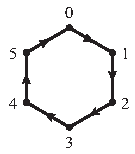
\includegraphics[width=\linewidth,height=.8\textheight,keepaspectratio]{assets/p090_00.pdf}\end{center}
\begin{center}\small\textbf{7.10 Figure}\end{center}\end{minipage}\hfill\begin{minipage}[t]{0.4903\linewidth}\vspace{0pt}\begin{center}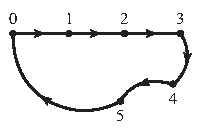
\includegraphics[width=\linewidth,height=.8\textheight,keepaspectratio]{assets/p090_02.pdf}\end{center}\end{minipage}
\end{center}
\end{BookFloat}

(a)

(b)

Two digraphs for \BookInline{\mathbb{Z}_{6}} with \BookInline{S= \{1\}} using

.

1

\begin{BookFloat}{07_generating_sets_and_cayley_digraphs-p90-6}
\begin{center}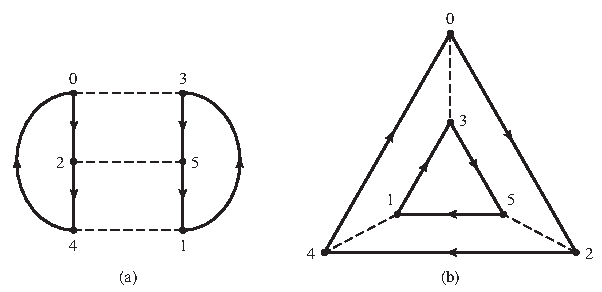
\includegraphics[width=0.826\linewidth,height=.8\textheight,keepaspectratio]{assets/review_v3_p090_7.11.pdf}\end{center}
\begin{center}\small \textbf{7.11 Figure}\quad Two digraphs for $\mathbb{Z}_6$ with $S=\{2,3\}$ using
\tikz[baseline=-.5ex]{\draw[->,thin] (0,0)--(12mm,0);\node[below=1pt,inner sep=0pt] at (6mm,0){\scriptsize $2$};}
and
\tikz[baseline=-.5ex]{\draw[->,thin,dashed] (0,0)--(12mm,0);\node[below=1pt,inner sep=0pt] at (6mm,0){\scriptsize $3$};}.\end{center}
\end{BookFloat}

\begin{BookFloat}{07_generating_sets_and_cayley_digraphs-p90-7}
\begin{center}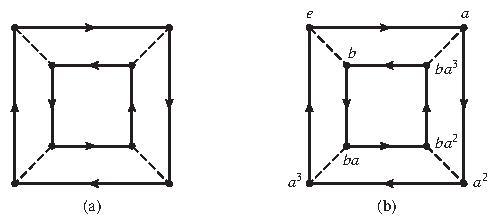
\includegraphics[width=0.680\linewidth,height=.8\textheight,keepaspectratio]{assets/review_v3_p090_7.13.pdf}\end{center}
\begin{center}\small \textbf{7.13 Figure}\end{center}
\end{BookFloat}

\BookTextHeading{\textit{\textbf{Property}}}

\BookTextHeading{\textit{\textbf{Reason}}}

1. The digraph is connected, that is, we can get from any vertex \BookInline{g} to any vertex \BookInline{h} by traveling along consecutive arcs, starting at \BookInline{g} and ending at \BookInline{h.}

Every equation \BookInline{gx= h} has a solution in a group.

2. At most one arc goes from a vertex \BookInline{g} to a vertex \BookInline{h.}

The solution of \BookInline{gx= h} is unique.

3. Each vertex \BookInline{g} has exactly one arc of each type starting at \BookInline{g,\allowbreak } and one of each type ending at \BookInline{g.}

For \BookInline{g\in G} and each generator \BookInline{b} we can compute \BookInline{gb,\allowbreak } and \BookInline{(gb^{- 1})b= g.}

4. If two different sequences of arc types starting from vertex \BookInline{g} lead to the same vertex \BookInline{h,\allowbreak } then those same sequences of arc types starting from any vertex \BookInline{u} will lead to the same vertex \BookInline{v.}

If \BookInline{gq= h} and\textit{ gr} \BookInline{= h,\allowbreak } then \BookInline{uq= } \BookInline{ug^{- 1}h= ur.}

\end{BookBody}

% Source PDF page 91; original printed page 74
\BookSource{91}{74}
\BookNarrativetrue

\begin{BookBody}

\noindent It can be shown that, conversely, every digraph satisfying these four properties is a Cayley digraph for some group. Due to the symmetry of such a digraph, we can choose labels like \BookInline{a,\allowbreak b,\allowbreak c} for the various arc types, name any vertex \BookInline{e} to represent the identity, and name each other vertex by a product of arc labels and their inverses that we can travel to attain that vertex starting from the one that we named \BookInline{e.} Some finite groups were first constructed (found) using digraphs.

\BookLabel{7.14 Example} A digraph satisfying the four properties given above is shown in Fig. 7.13 (a). To obtain Fig. 7.13 (b), we selected the labels

\begin{center}\begin{adjustbox}{max width=\linewidth}\BookInline{\displaystyle \xrightarrow{\quad\quad}\quad  and  \quad \xrightarrow{\quad\quad}\quad \xrightarrow{\quad\quad}}\end{adjustbox}\end{center}

\noindent named a vertex \BookInline{e,\allowbreak } and then named the other vertices as shown. We have a group

\begin{center}\begin{adjustbox}{max width=\linewidth}\BookInline{\displaystyle \{e,\allowbreak a,\allowbreak a^{2},\allowbreak a^{3},\allowbreak b,\allowbreak ba,\allowbreak ba^{2},\allowbreak ba^{3}\}}\end{adjustbox}\end{center}

\noindent of eight elements. From the diagram we could compute any product. For example, to compute \BookInline{ba^{2}ba^{3}} we start at the vertex labeled \BookInline{ba^{2},\allowbreak } follow a dotted edge, and then follow three solid edges to arrive at \BookInline{a.} Note that the way we labeled the vertices is not unique. For example, the vertex labeled \BookInline{ba^{3}} could have been labeled \BookInline{ab} simply by going along a different path starting at \BookInline{e.} This says that \BookInline{ab= ba^{3}.} We also see that \BookInline{a^{4}= e} and \BookInline{b^{2}= e.} We hope that this example is starting to look familiar. In fact, Figure 7.13 is a Cayley digraph of the dihedral group \BookInline{D_{4}.} We simply relabel \BookInline{a} with \BookInline{\rho } and \BookInline{b} with \BookInline{\mu }! \BookEnd{\blacktriangle}

\end{BookBody}

\BookNarrativefalse

\begin{BookBody}

\BookExerciseTitle{7}

\BookTextHeading{\textbf{Computations}}

\noindent In Exercises 1 through 8, list the elements of the subgroup generated by the given subset.

\BookExercise{1.}{The subset \BookInline{\{2,\allowbreak 3\}} of \BookInline{\mathbb{Z}_{12}}}

\BookExercise{2.}{The subset \BookInline{\{4,\allowbreak 6\}} of \BookInline{\mathbb{Z}_{12}}}

\BookExercise{3.}{The subset \BookInline{\{4,\allowbreak 6\}} in \BookInline{\mathbb{Z}_{25}}}

\BookExercise{4.}{The subset \BookInline{\{12,\allowbreak 30\}} of \BookInline{\mathbb{Z}_{36}}}

\BookExercise{5.}{The subset \BookInline{\{12,\allowbreak 42\}} of \BookInline{\mathbb{Z}}}

\BookExercise{6.}{The subset \BookInline{\{18,\allowbreak 24,\allowbreak 39\}} of \BookInline{\mathbb{Z}}}

\BookExercise{7.}{The subset \BookInline{\{\mu,\allowbreak \mu \rho ^{2}\}} in \BookInline{D_{8}}}

\BookExercise{8.}{The subset \BookInline{\{\rho ^{8},\allowbreak \rho ^{10}\}} in \BookInline{D_{18}}}

\BookExercise{9.}{Use the Cayley digraph in Figure 7.15 to compute these products. Note that the solid edges represent the generator \BookInline{a} and the dashed lines represent \BookInline{b.} \textbf{a}\BookInline{.(ba^{2})a^{3}} \textbf{b}\BookInline{.(ba)(ba^{3})} \textbf{c}\BookInline{.b(a^{2}b)}}

\begin{BookFloat}{07_generating_sets_and_cayley_digraphs-p91-18}
\begin{center}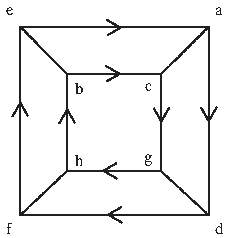
\includegraphics[width=0.312\linewidth,height=.8\textheight,keepaspectratio]{assets/p091_15.pdf}\end{center}
\begin{center}\small\textbf{7.15 Figure}\end{center}
\end{BookFloat}

\end{BookBody}

% Source PDF page 92; original printed page 75
\BookSource{92}{75}
\BookNarrativefalse

\begin{BookBody}

\noindent In Exercises 10 through 12, give the table for the group having the indicated digraph. In each digraph, take \BookInline{e} as identity element. List the identity \BookInline{e} first in your table, and list the remaining elements alphabetically, so that your answers will be easy to check.

\BookExercise{10.}{The digraph in Fig. 7.16(a)}

\BookExercise{11.}{The digraph in Fig. 7.16(b)}

\BookExercise{12.}{The digraph in Fig. 7.16(c)}

\begin{BookFloat}{07_generating_sets_and_cayley_digraphs-p92-4}
\begin{center}
\begin{minipage}[t]{0.2053\linewidth}\vspace{0pt}\begin{center}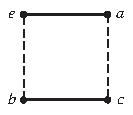
\includegraphics[width=\linewidth,height=.8\textheight,keepaspectratio]{assets/p092_04.pdf}\end{center}\end{minipage}\hfill\begin{minipage}[t]{0.2541\linewidth}\vspace{0pt}\begin{center}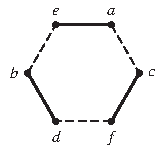
\includegraphics[width=\linewidth,height=.8\textheight,keepaspectratio]{assets/p092_06.pdf}\end{center}
\begin{center}\small\textbf{7.16 Figure}\end{center}\end{minipage}\hfill\begin{minipage}[t]{0.3659\linewidth}\vspace{0pt}\begin{center}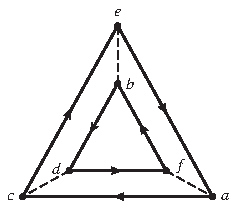
\includegraphics[width=\linewidth,height=.8\textheight,keepaspectratio]{assets/p092_09.pdf}\end{center}\end{minipage}
\end{center}
\end{BookFloat}

(a)

(b)

(c)

\BookTextHeading{\textbf{Concepts}}

\BookExercise{13.}{How can we tell from a Cayley digraph whether or not the corresponding group is commutative?}

\BookExercise{14.}{Using the condition found in Exercise 13, show that the group corresponding to the Cayley digraph in Figure 7.13 is not commutative.}

\BookExercise{15.}{Is it obvious from a Cayley digraph of a group whether or not the group is cyclic? [\textit{Hint:} Look at Fig. 7.9(b).]}

\BookExercise{16.}{The large outside triangle in Fig. 7.11(b) exhibits the cyclic subgroup \BookInline{\{0,\allowbreak 2,\allowbreak 4\}} of \BookInline{\mathbb{Z}_{6}.} Does the smaller inside triangle similarly exhibit a cyclic subgroup of \BookInline{\mathbb{Z}_{6}}? Why or why not?}

\BookExercise{17.}{The generating set \BookInline{S= \{1,\allowbreak 2\}} for \BookInline{\mathbb{Z}_{6}} contains more generators than necessary, since 1 is a generator for the group. Nevertheless, we can draw a Cayley digraph for \BookInline{\mathbb{Z}_{6}} with this generating set \BookInline{S.} Draw such a Cayley digraph.}

\BookExercise{18.}{Draw a Cayley digraph for \BookInline{\mathbb{Z}_{8}} with generating set \BookInline{S= \{2,\allowbreak 5\}.}}

\BookExercise{19.}{A\textbf{ relation} on a set \BookInline{S} of generators of a group \BookInline{G} is an equation that equates some product of generators and their inverses to the identity \BookInline{e} of \BookInline{G.} For example, if \BookInline{S= \{a,\allowbreak b\}} and \BookInline{G} is commutative so that \BookInline{ab= ba,\allowbreak } then one relation is \BookInline{aba^{- 1}b^{- 1}= e.} If, moreover\BookInline{,\allowbreak b} is its own inverse, then another relation is \BookInline{b^{2}= e.}}

\BookExercise{a.}{Explain how we can find some relations on \BookInline{S} from a Cayley digraph of \BookInline{G.}}

\BookExercise{b.}{Find three relations on the set \BookInline{S= \{a,\allowbreak b\}} of generators for the group described by Fig. 7.13(b).}

\BookExercise{20.}{Draw digraphs of the two possible structurally different groups of order 4, taking as small a generating set as possible in each case. You need not label vertices.}

\BookTextHeading{\textbf{Theory}}

\BookExercise{21.}{Use Cayley digraphs to show that for \BookInline{n\geq 3,\allowbreak } there exists a nonabelian group with \BookInline{2n} elements that is generated by two elements of order 2.}

\BookExercise{22.}{Prove that there are at least three different abelian groups of order 8. [Hint: Find a Cayley digraph for a group of order 8 having one generator of order 4 and another of order 2. Find a second Cayley digraph for a group of order 8 having three generators each with order 2.]}

\end{BookBody}
\ifdefined\BookMaster\let\BookFinish\relax\else\def\BookFinish{\end{document}}\fi\BookFinish

\clearpage
% !TeX program = xelatex
\ifdefined\BookMaster\else
\documentclass[11pt,oneside]{article}
% !TeX program = xelatex
\usepackage[b5paper,left=22mm,right=22mm,top=20mm,bottom=22mm,footskip=11mm]{geometry}
\usepackage{fontspec}
\setmainfont{TeX Gyre Termes}
\setsansfont{TeX Gyre Heros}
\usepackage{amsmath,amssymb,mathtools,amsthm}
\renewcommand{\cdots}{\mathinner{\cdotp\cdotp\cdotp}}
\usepackage{graphicx,adjustbox,array,booktabs,longtable,multirow,enumitem,changepage,needspace}
\usepackage[table]{xcolor}
\usepackage{fancyhdr}
\raggedbottom
\interfootnotelinepenalty=10000
\newcommand{\BookFootnote}[2]{\begingroup\renewcommand{\thefootnote}{\fnsymbol{footnote}}\footnote[#1]{#2}\endgroup}
\newcommand{\BookFootnoteMark}[1]{\begingroup\renewcommand{\thefootnote}{\fnsymbol{footnote}}\footnotemark[#1]\endgroup}
\newcommand{\BookFootnoteText}[2]{\begingroup\renewcommand{\thefootnote}{\fnsymbol{footnote}}\footnotetext[#1]{#2}\endgroup}
\newenvironment{BookFloat}[1]{\par\addvspace{.6\baselineskip}\noindent\def\BookFloatID{#1}\begin{minipage}{\linewidth}\phantomsection\label{bookfloat:#1:start}}{\phantomsection\label{bookfloat:\BookFloatID:end}\end{minipage}\par\addvspace{.6\baselineskip}}

\usepackage[unicode,hidelinks]{hyperref}
\pagestyle{fancy}
\fancyhf{}
\newcommand{\BookFooter}{}
\fancyfoot[L]{\parbox[b]{\dimexpr\textwidth-15mm}{\footnotesize\BookFooter}}
\fancyfoot[R]{\footnotesize\thepage}
\renewcommand{\headrulewidth}{0pt}
\renewcommand{\footrulewidth}{0pt}
\setlength{\parindent}{0pt}
\setlength{\parskip}{0.2em}
\setlength{\emergencystretch}{3em}
\setlist{nosep,leftmargin=1.7em,labelsep=.65em}
\newif\ifBookNarrative
\BookNarrativetrue
\newenvironment{BookBody}{\setlength{\parindent}{0pt}}{}
\newcommand{\BookStatement}[1]{\par\addvspace{.6\baselineskip}\noindent #1\enspace\ignorespaces}
\newcommand{\BookLabel}[1]{\par\addvspace{.6\baselineskip}\needspace{3\baselineskip}\noindent\textbf{#1}\quad\ignorespaces}
\newcommand{\BookHeading}[1]{\par\addvspace{\baselineskip}\needspace{4\baselineskip}\noindent{\large\bfseries #1}\par\medskip}
\newcommand{\BookSubheading}[1]{\par\addvspace{.7\baselineskip}\needspace{3\baselineskip}\noindent{\bfseries #1}\par\smallskip}
\newcommand{\BookTextHeading}[1]{\par\addvspace{.7\baselineskip}\needspace{3\baselineskip}\noindent #1\par\smallskip}
\newcommand{\BookSectionTitle}[2]{\par\addvspace{1.2\baselineskip}\needspace{5\baselineskip}\noindent\colorbox{gray!25}{\sffamily\bfseries\small SECTION #1}\quad{\large\bfseries #2}\par\medskip}
\newcommand{\BookExerciseTitle}[1]{\par\addvspace{\baselineskip}\needspace{4\baselineskip}\noindent{\color{gray}\rule{1.5mm}{1.5mm}}\enspace{\large\bfseries Exercises #1}\par\medskip}
\newcommand{\BookBullet}[1]{\begin{list}{\textbullet}{\setlength{\leftmargin}{1.7em}\setlength{\labelwidth}{1em}\setlength{\labelsep}{.7em}\setlength{\topsep}{0pt}\setlength{\parsep}{0pt}\setlength{\itemsep}{0pt}}\item #1\end{list}}
\newcommand{\BookExercise}[2]{\begin{list}{\textbf{#1}}{\setlength{\leftmargin}{2.2em}\setlength{\labelwidth}{1.5em}\setlength{\labelsep}{.7em}\setlength{\topsep}{.15em}\setlength{\parsep}{0pt}\setlength{\itemsep}{0pt}}\item #2\end{list}}
\newcommand{\BookEnd}[1]{\unskip\nobreak\hfill\ensuremath{#1}}
\newcommand{\BookSource}[2]{\phantomsection\label{sourcepage:#1}} % Source-page anchors, retained through reflow.
\usepackage{multicol}
\usepackage{tikz}
\newcommand{\BookPartEntry}[2]{\par\noindent\makebox[17mm][l]{\bfseries Section #1}#2\par}
\newcommand{\BookPartTitle}[3]{\par\bigskip\noindent\begin{tikzpicture}\node[anchor=north west,inner sep=0pt,outer sep=0pt] (bookpart) at (0,0) {\begin{minipage}{\dimexpr\linewidth-.5pt}\hspace*{26mm}\begin{minipage}[t]{\dimexpr\linewidth-26mm}\begin{adjustbox}{max width=\linewidth}{\fontsize{20}{24}\selectfont\bfseries #2}\end{adjustbox}\par\vspace{6mm}\hrule\vspace{6mm}{\sffamily\footnotesize\setlength{\parskip}{.3em}#3}\vspace{3mm}\end{minipage}\end{minipage}};\path[shade,top color=gray!60,bottom color=white] (0,0) rectangle ([xshift=24mm]bookpart.south west);\node[anchor=north,font=\sffamily\bfseries\small] at (12mm,-2mm) {PART};\node[anchor=north,font=\sffamily\bfseries\Huge] at (12mm,-7mm) {#1};\end{tikzpicture}\par\bigskip}
\newsavebox{\BookMathBox}
\makeatletter
\newcommand{\BookInline}[1]{\leavevmode\hskip0pt\relax\begingroup\in@{\begin}{#1}\ifin@\sbox{\BookMathBox}{\(#1\)}\ifdim\wd\BookMathBox>\dimexpr\linewidth-1em\relax\resizebox{\dimexpr\linewidth-1em\relax}{!}{\usebox{\BookMathBox}}\else\(#1\)\fi\else\in@{\left}{#1}\ifin@\sbox{\BookMathBox}{\(#1\)}\ifdim\wd\BookMathBox>\dimexpr\linewidth-1em\relax\resizebox{\dimexpr\linewidth-1em\relax}{!}{\usebox{\BookMathBox}}\else\(#1\)\fi\else\(#1\)\fi\fi\endgroup\hskip0pt\relax}
\makeatother
\DeclareMathOperator{\Aut}{Aut}
\DeclareMathOperator{\End}{End}
\DeclareMathOperator{\Hom}{Hom}
\DeclareMathOperator{\GF}{GF}
\DeclareMathOperator{\irr}{irr}
\DeclareMathOperator{\lt}{lt}
\DeclareMathOperator{\lp}{lp}
\providecommand{\textcircled}[1]{\textnormal{(#1)}}

\begin{document}
\fi
\renewcommand{\BookFooter}{Section 8 Groups of Permutations}
\pdfbookmark[0]{Section 8 Groups of Permutations}{08_groups_of_permutations}
\ifdefined\BookMaster\else\setcounter{page}{77}\fi
% Source PDF page 94; original printed page 77
\BookSource{94}{77}
\BookPartTitle{II}{Structure of Groups}{\BookPartEntry{8}{Groups of Permutations}
\BookPartEntry{9}{Finitely Generated Abelian Groups}
\BookPartEntry{10}{Cosets and the Theorem of Lagrange}
\BookPartEntry{11}{Plane Isometries}}

\BookNarrativetrue

\begin{BookBody}

\BookSectionTitle{8}{Groups of Permutations}

\noindent Let \BookInline{\phi:G\to G^{\prime }} be a function mapping the group \BookInline{G} to \BookInline{G^{\prime }.} Recall that the homomorphism property of an isomorphism states that for all \BookInline{a,\allowbreak b\in G,\allowbreak \phi (ab)= \phi (a)\phi (b).} Whenever a function has this property whether or not the function is one-to-one or onto, we say that \BookInline{\phi } is a\textbf{ group homomorphism}. Of course any group isomorphism is a group homomorphism, but the reverse is not necessarily true.

\BookLabel{8.1 Definition} Let \BookInline{G} and \BookInline{G^{\prime }} be groups with \BookInline{\phi:G\to G^{\prime }.} The map \BookInline{\phi } is a\textbf{ homomorphism} if the homomorphism property

\begin{center}\begin{adjustbox}{max width=\linewidth}\BookInline{\displaystyle \phi (ab)= \phi (a)\phi (b)}\end{adjustbox}\end{center}

\noindent holds for all \BookInline{a,\allowbreak b\in G.} \BookEnd{\blacksquare}

\BookLabel{8.2 Example} Let \BookInline{\phi:\mathbb{R}\to U(}the circle group) be defined by the formula

\begin{center}\begin{adjustbox}{max width=\linewidth}\BookInline{\displaystyle \phi (x)= \;\text{cos}\;(2\pi x)+ i\;\text{sin}\;(2\pi x)= e^{2\pi ix}.}\end{adjustbox}\end{center}

\noindent Then

\begin{center}\begin{adjustbox}{max width=\linewidth}\BookInline{\displaystyle \phi (a+ b)= \;\text{cos}\;(2\pi (a+ b))+ i\;\text{sin}\;(2\pi (a+ b))= e^{2\pi i(a+ b)}.}\end{adjustbox}\end{center}

\noindent Using either the usual properties of the exponential function or the formulas from trigonometry involving the sum of two angles, we see that

\begin{center}\begin{adjustbox}{max width=\linewidth}\BookInline{\displaystyle \phi (a+ b)= (\;\text{cos}\;(2\pi a)+ i\;\text{sin}\;(2\pi a))(\;\text{cos}\;(2\pi b)+ i\;\text{sin}\;(2\pi b))= e^{2\pi ai}e^{2\pi bi},\allowbreak }\end{adjustbox}\end{center}

\noindent so

\begin{center}\begin{adjustbox}{max width=\linewidth}\BookInline{\displaystyle \phi (a+ b)= \phi (a)\phi (b),\allowbreak }\end{adjustbox}\end{center}

\noindent which says that \BookInline{\phi } is a group homomorphism. Although \BookInline{\phi } maps onto \BookInline{U,\allowbreak } it is not one-toone, so \BookInline{\phi } is not an isomorphism.

The identity \BookInline{0\in \mathbb{R}} maps to 1, the identity in \BookInline{U.} Furthermore, for any \BookInline{x\in \mathbb{R},\allowbreak }

\begin{center}\begin{adjustbox}{max width=\linewidth}\BookInline{\displaystyle \phi ( - x ) = e ^ { - 2 \pi i x } = { \frac { 1 } { e ^ { 2 \pi i x } } } = ( \phi ( x ) ) ^ { - 1 } .}\end{adjustbox}\end{center} \BookEnd{\blacktriangle}

\end{BookBody}

% Source PDF page 95; original printed page 78
\BookSource{95}{78}
\BookNarrativetrue

\begin{BookBody}

\BookLabel{8.3 Example} Recall that \BookInline{U_{n}= \{z\in \mathbb{C}\mid z^{n}= 1\}.} Let \BookInline{\phi:U_{28}\to U_{4}} be given by \BookInline{\phi (z)= z^{7}.} To check that \BookInline{\phi } is well defined, we see that if \BookInline{z\in U_{28},\allowbreak } then \BookInline{z^{28}= 1.} Therefore\BookInline{,\allowbreak (z^{7})^{4}= 1,\allowbreak } which implies that \BookInline{z^{7}\in U_{4}.} We check that \BookInline{\phi } is a homomorphism.

\begin{center}\begin{adjustbox}{max width=\linewidth}\BookInline{\displaystyle \phi (z_{1}z_{2})= (z_{1}z_{2})^{7}= z_{1}^{7}z_{2}^{7}= \phi (z_{1})\phi (z_{2}).}\end{adjustbox}\end{center}

\noindent As in the previous example\BookInline{,\allowbreak \phi } maps the identity in \BookInline{U_{28},\allowbreak } in this case 1, to the identity 1 in \BookInline{U_{4}.} Furthermore,

\begin{center}\begin{adjustbox}{max width=\linewidth}\BookInline{\displaystyle \phi (z^{- 1})= z^{- 7}= (z^{7})^{- 1}= (\phi (z))^{- 1}.}\end{adjustbox}\end{center} \BookEnd{\blacktriangle}

\BookLabel{8.4 Definition} Let \BookInline{\phi:X\to Y} and suppose that \BookInline{A\subseteq X} and \BookInline{B\subseteq Y.} The set \BookInline{\phi [A]= \{\phi (a)\mid a\in A\}} is called the\textbf{ image of} \BookInline{A} \textbf{in} \BookInline{Y} \textbf{under the mapping} \BookInline{\phi.} The set \BookInline{\phi ^{- 1}[B]= \{a\in A\mid \phi (a)\in B\}} is called the\textbf{ inverse image of} \BookInline{B} \textbf{under the mapping} \BookInline{\phi.}\BookEnd{\blacksquare}

\noindent The four properties of a homomorphism given in the theorem that follows are obvious in the case of an isomorphism since we think of an isomorphism as simply relabeling the elements of a group. However, it is not obvious that these properties hold for all homomorphisms whether or not they are one-to-one or onto maps. Consequently, we give careful proofs of all four properties.

\BookLabel{8.5 Theorem} Let \BookInline{\phi } be a homomorphism of a group \BookInline{G} into a group \BookInline{G^{\prime }.}

\BookExercise{1.}{If \BookInline{e} is the identity element in \BookInline{G,\allowbreak } then \BookInline{\phi (e)} is the identity element \BookInline{e^{\prime }} in \BookInline{G^{\prime }.}}

\BookExercise{2.}{If \BookInline{a\in G,\allowbreak } then \BookInline{\phi (a^{- 1})= \phi (a)^{- 1}.}}

\BookExercise{3.}{If \BookInline{H} is a subgroup of \BookInline{G,\allowbreak } then \BookInline{\phi [H]} is a subgroup of \BookInline{G^{\prime }.}}

\BookExercise{4.}{If \BookInline{K^{\prime }} is a subgroup of \BookInline{G^{\prime },\allowbreak } then \BookInline{\phi ^{- 1}[K^{\prime }]} is a subgroup of \BookInline{G.}}

\noindent Loosely speaking\BookInline{,\allowbreak \phi } preserves the identity element, inverses, and subgroups.

\BookLabel{\textit{Proof}} Let \BookInline{\phi } be a homomorphism of \BookInline{G} into \BookInline{G^{\prime }.} Then

\begin{center}\begin{adjustbox}{max width=\linewidth}\BookInline{\displaystyle \phi (e)= \phi (ee)= \phi (e)\phi (e).}\end{adjustbox}\end{center}

\noindent Multiplying on the left by \BookInline{\phi (e)^{- 1},\allowbreak } we see that \BookInline{e^{\prime }= \phi (e).} Thus \BookInline{\phi (e)} must be the identity element \BookInline{e^{\prime }} in \BookInline{G^{\prime }.} The equation

\begin{center}\begin{adjustbox}{max width=\linewidth}\BookInline{\displaystyle e^{\prime }= \phi (e)= \phi (aa^{- 1})= \phi (a)\phi (a^{- 1})}\end{adjustbox}\end{center}

\noindent shows that \BookInline{\phi (a^{- 1})= \phi (a)^{- 1}} for all \BookInline{a\in G.}

Turning to Statement (3), let \BookInline{H} be a subgroup of \BookInline{G,\allowbreak } and let \BookInline{\phi (a)} and \BookInline{\phi (b)} be any two elements in \BookInline{\phi [H].} Then \BookInline{\phi (a)\phi (b)= \phi (ab),\allowbreak } so we see that \BookInline{\phi (a)\phi (b)\in \phi [H];} thus, \BookInline{\phi [H]} is closed under the operation of \BookInline{G^{\prime }.} The fact that \BookInline{e^{\prime }= \phi (e)} and \BookInline{\phi (a^{- 1})= \phi (a)^{- 1}} completes the proof that \BookInline{\phi [H]} is a subgroup of \BookInline{G^{\prime }.}

Going the other way for Statement (4), let \BookInline{K^{\prime }} be a subgroup of \BookInline{G^{\prime }.} Suppose \BookInline{a} and \BookInline{b} are in \BookInline{\phi ^{- 1}[K^{\prime }].} Then \BookInline{\phi (a)\phi (b)\in K^{\prime }} since \BookInline{K^{\prime }} is a subgroup. The equation \BookInline{\phi (ab)= } \BookInline{\phi (a)\phi (b)} shows that \BookInline{ab\in \phi ^{- 1}[K^{\prime }].} Thus \BookInline{\phi ^{- 1}[K^{\prime }]} is closed under the binary operation in \BookInline{G.} Also\BookInline{,\allowbreak K^{\prime }} must contain the identity element \BookInline{e^{\prime }= \phi (e),\allowbreak } so \BookInline{e\in \phi ^{- 1}[K^{\prime }].} If \BookInline{a\in \phi ^{- 1}[K^{\prime }],\allowbreak } then \BookInline{\phi (a)\in K^{\prime },\allowbreak } so \BookInline{\phi (a)^{- 1}\in K^{\prime }.} But \BookInline{\phi (a)^{- 1}= \phi (a^{- 1}),\allowbreak } so we must have \BookInline{a^{- 1}\in \phi ^{- 1}[K^{\prime }].} Hence \BookInline{\phi ^{- 1}[K^{\prime }]} is a subgroup of \BookInline{G.}\BookEnd{\blacklozenge}

Let \BookInline{\phi:G\to G^{\prime }} be a homomorphism and let \BookInline{e^{\prime }} be the identity element of \BookInline{G^{\prime }.} Now \BookInline{\{e^{\prime }\}} is a subgroup of \BookInline{G^{\prime },\allowbreak } so \BookInline{\phi ^{- 1}[\{e^{\prime }\}]} is a subgroup \BookInline{H} of \BookInline{G} by Statement (4) in Theorem 8.5. This subgroup is critical to the study of homomorphisms.

\BookLabel{8.6 Definition} Let \BookInline{\phi:G\to G^{\prime }} be a homomorphism of groups. The subgroup \BookInline{\phi ^{- 1}[\{e^{\prime }\}]= } \BookInline{\{x\in G\mid \phi (x)= e^{\prime }\}} is the\textbf{ kernel of} \BookInline{\phi,\allowbreak } denoted by Ker\BookInline{(\phi ).}\BookEnd{\blacksquare}

\end{BookBody}

% Source PDF page 96; original printed page 79
\BookSource{96}{79}
\BookNarrativetrue

\begin{BookBody}

We will use the kernel of a homomorphism when we define the alternating group later in this section.

Another extreme is to let \BookInline{H= G} in Statement (3) of Theorem 8.5. In this case, the theorem says that \BookInline{\phi [G]} is a subgroup of \BookInline{G^{\prime }.} We use this in the proof of Cayley’s Theorem.

\BookLabel{8.7 Example} In Example 8.2, the homomorphism \BookInline{\phi:\mathbb{R}\to U} is defined by \BookInline{\phi (x)= } cos\BookInline{(2\pi x)+ } \BookInline{i} sin\BookInline{(2\pi x)= e^{2\pi }}\textit{ix}. The kernel of \BookInline{\phi } is the set of integers since cos\BookInline{(2\pi x)+ i} sin\BookInline{(2\pi x)= 1} if and only if \BookInline{x} is an integer.

Let \BookInline{n} be a positive integer. Then \BookInline{\left\langle { \frac { 1 } { n } } \right\rangle} is a subgroup of \BookInline{\mathbb{R}} and

\begin{center}\begin{adjustbox}{max width=\linewidth}\BookInline{\displaystyle \begin{aligned} \phi \left[ \left\langle \frac{1}{n} \right\rangle \right] &= \phi \left[ \left\{ \frac{m}{n} \left|   m \in \mathbb{Z} \right\} \right. \right] \\&= \left\{ \cos(2\pi m/n + i \sin(2\pi m/n)) \left|   m \in \mathbb{Z} \right\} \right. \\&= U_n.\\ \end{aligned}}\end{adjustbox}\end{center} \BookEnd{\blacktriangle}

\BookLabel{8.8 Example} Let \BookInline{\phi:\mathbb{Z}_{n}\to D_{n}} be given by \BookInline{\phi (k)= \rho ^{k}.} We check that \BookInline{\phi } is a homomorphism. Let \BookInline{a,\allowbreak b\in \mathbb{Z}_{n}.} If \BookInline{a+ b<n,\allowbreak } then \BookInline{a+ _{n}b= a+ b,\allowbreak } so \BookInline{\phi (a+ _{n}b)= \phi (a+ b)= \rho ^{a+ b}= \rho ^{a}\rho ^{b}} \BookInline{= \phi (a)\phi (b).} If \BookInline{a+ b\geq n,\allowbreak } then \BookInline{\phi (a+ _{n}b)= \phi (a+ b- n)= \rho ^{a+ b- n}= \rho ^{a}\rho ^{b}\rho ^{- n}= } \BookInline{\rho ^{a}\rho ^{b}= \phi (a)\phi (b).} The image \BookInline{\phi [\mathbb{Z}_{n}]} is \BookInline{\langle \rho \rangle.}\BookEnd{\blacktriangle}

\BookTextHeading{\textbf{Cayley’s Theorem}  }

\noindent Each of the groups we have seen so far is isomorphic to a subgroup of permutations on some set. For example\BookInline{,\allowbreak \mathbb{Z}_{n}} is isomorphic with the cyclic group \BookInline{\langle (1,\allowbreak 2,\allowbreak 3,\allowbreak...,\allowbreak n)\rangle \leq S_{n}.} The dihedral group \BookInline{D_{n}} is defined to be the permutations in \BookInline{S_{\mathbb{Z}_{n}}} with the property that the line segment between vertices \BookInline{i} and \BookInline{j} is an edge in \BookInline{P_{n},\allowbreak } a regular \BookInline{n-}gon, if and only if the line segment between the images of \BookInline{i} and \BookInline{j} is also an edge. The infinite group GL\BookInline{(n,\allowbreak \mathbb{R})} can be thought of as invertible linear transformations of \BookInline{\mathbb{R}^{n}.} Each element of GL\BookInline{(n,\allowbreak \mathbb{R})} permutes the vectors in \BookInline{\mathbb{R}^{n},\allowbreak } which makes GL\BookInline{(n,\allowbreak \mathbb{R})} isomorphic with a permutation group on vectors in \BookInline{\mathbb{R}^{n}.} We refer to a subgroup of a permutation group as a\textbf{ group} \textbf{of permutations}. Cayley’s Theorem states that any group is isomorphic with a group of permutations.

At first Cayley’s Theorem seems like a remarkable result that could be used to understand all groups. In fact, this is a nice and intriguing classic result. Unfortunately, approaching group theory by trying to determine all possible permutation groups is not feasible. On the other hand, Cayley’s theorem does show the strength and generality of permutation groups and it deserves a special place in group theory for that reason. For example, if we wish to find a counterexample to a conjecture about groups, provided that there is one, it will occur in a permutation group.

It may seem a mystery how we could start with an arbitrary group and come up with a permutation group that is isomorphic with the given group. The key is to think about the group table. Each row contains each element of the group exactly once. So each row defines a permutation of the elements of the group by placing the table head as the top row in the two-row representation of a permutation and placing the row corresponding to an element \BookInline{a} in the group as the bottom row. Table 8.9 is the group table for \BookInline{D_{3}.} Note that the permutation obtained using the row \BookInline{\mu \rho } is

\begin{center}\begin{adjustbox}{max width=\linewidth}\BookInline{\displaystyle \begin{pmatrix}\iota & \rho & \rho^2 & \mu & \mu\rho & \mu\rho^2 \\\mu\rho & \mu\rho^2 & \mu & \rho^2 & \iota & \rho\end{pmatrix}.}\end{adjustbox}\end{center}

\end{BookBody}

% Source PDF page 97; original printed page 80
\BookSource{97}{80}
\BookNarrativetrue

\begin{BookBody}

\begin{BookFloat}{08_groups_of_permutations-p97-0}
\begin{center}\small\textbf{8.9 Table}\end{center}
\begin{center}\begin{adjustbox}{max width=\linewidth}
\renewcommand{\arraystretch}{1.2}\setlength{\tabcolsep}{5pt}
\begin{tabular}{c|cccccc}
\BookInline{D_{3}} & \BookInline{\iota } & \BookInline{\rho } & \BookInline{\rho ^{2}} & \BookInline{\mu } & \BookInline{\mu \rho } & \BookInline{\mu \rho ^{2}}\\\hline
\BookInline{\iota } & \BookInline{\iota } & \BookInline{\rho } & \BookInline{\rho ^{2}} & \BookInline{\mu } & \BookInline{\mu \rho } & \BookInline{\mu \rho ^{2}}\\
\BookInline{\rho } & \BookInline{\rho } & \BookInline{\rho ^{2}} & \BookInline{\iota } & \BookInline{\mu \rho ^{2}} & \BookInline{\mu } & \BookInline{\mu \rho }\\
\BookInline{\rho ^{2}} & \BookInline{\rho ^{2}} & \BookInline{\iota } & \BookInline{\rho } & \BookInline{\mu \rho } & \BookInline{\mu \rho ^{2}} & \BookInline{\mu }\\
\BookInline{\mu } & \BookInline{\mu } & \BookInline{\mu \rho } & \BookInline{\mu \rho ^{2}} & \BookInline{\iota } & \BookInline{\rho } & \BookInline{\rho ^{2}}\\
\BookInline{\mu \rho } & \BookInline{\mu \rho } & \BookInline{\mu \rho ^{2}} & \BookInline{\mu } & \BookInline{\rho ^{2}} & \BookInline{\iota } & \BookInline{\rho }\\
\BookInline{\mu \rho ^{2}} & \BookInline{\mu \rho ^{2}} & \BookInline{\mu } & \BookInline{\mu \rho } & \BookInline{\rho } & \BookInline{\rho ^{2}} & \BookInline{\iota }\\
\end{tabular}
\end{adjustbox}\end{center}
\end{BookFloat}

All that remains to prove Cayley’s Theorem, at least when the group is finite, is to check that the permutations obtained from the group table form a group isomorphism with the original group. Let \BookInline{\lambda _{x}} be the permutation of the elements of \BookInline{G} given by the \BookInline{x} row of the table for \BookInline{G.} Then for any \BookInline{g\in G,\allowbreak \lambda _{x}(g)} is the entry in the \BookInline{x} row and \BookInline{g} column of the group table. In other words\BookInline{,\allowbreak \lambda _{x}(g)= xg,\allowbreak } which is perfectly valid in the case of an infinite as well as a finite group. We formalize this connection between \BookInline{G} and permutations on \BookInline{G} in Definition 8.10.

\BookLabel{8.10 Definition} Let \BookInline{G} be a group. The function \BookInline{\phi:G\to S_{G}} given by \BookInline{\phi (x)= \lambda _{x}} where \BookInline{\lambda _{x}(g)= xg} for all \BookInline{g\in G} is called the\textbf{ left regular representation} of \BookInline{G.}\BookEnd{\blacksquare}

\noindent In order to be sure that \BookInline{\lambda _{x}} is a permutation, it should be verified that \BookInline{\lambda _{x}} is both one-to-one and onto. We see that \BookInline{\lambda _{x}} is one-to-one since if \BookInline{\lambda _{x}(a)= \lambda _{x}(b),\allowbreak xa= xb} and cancellation gives \BookInline{a= b.} Also\BookInline{,\allowbreak \lambda _{x}} maps onto \BookInline{G} because for any \BookInline{b\in G,\allowbreak \lambda _{x}(x^{- 1}b))= b.} We are now ready to prove Cayley’s Theorem.

\BookLabel{8.11 Theorem} \textbf{(Cayley’s Theorem)} Every group is isomorphic to a group of permutations.

\BookLabel{\textit{Proof}} Let \BookInline{G} be a group. The left regular representation provides a map \BookInline{\phi:G\to S_{G}} defined by \BookInline{\phi (x)= \lambda _{x}.} We must verify that \BookInline{\phi } is a group homomorphism and that \BookInline{\phi } is one-to-one. Then \BookInline{\phi [G]} is a subgroup of \BookInline{S_{G}} by Theorem 8.5 and \BookInline{\phi:G\to \phi [G]} is an isomorphism.

We first show that \BookInline{\phi } is one-to-one. Suppose that \BookInline{a,\allowbreak b\in G} and \BookInline{\phi (a)= \phi (b).} Then the permutations \BookInline{\lambda _{a}} and \BookInline{\lambda _{b}} are the same, so \BookInline{\lambda _{a}(e)= \lambda _{b}(e).} Thus \BookInline{ae= } \textit{be} and \BookInline{a= b.} So \BookInline{\phi } is one-to-one.

We now need to show that \BookInline{\phi } is a group homomorphism. Let \BookInline{a,\allowbreak b\in G.} Then \BookInline{\phi (ab)= } \BookInline{\lambda _{ab}} and \BookInline{\phi _{a}\phi _{b}= \lambda _{a}\lambda _{b}.} We must show that the two permutations \BookInline{\lambda _{ab}} and \BookInline{\lambda _{a}\lambda _{b}} are the same. Let \BookInline{g\in G.}

\begin{center}\begin{adjustbox}{max width=\linewidth}\BookInline{\displaystyle \lambda _{ab}(g)= (ab)g= a(bg)= \lambda _{a}(bg)= \lambda _{a}(\lambda _{b}(g))= (\lambda _{a}\lambda _{b})(g).}\end{adjustbox}\end{center}

\noindent Thus \BookInline{\lambda _{ab}= \lambda _{a}\lambda _{b},\allowbreak } which implies that \BookInline{\phi (ab)= \phi (a)\phi (b).} So \BookInline{\phi } is a one-to-one homomorphism, which completes the proof\BookInline{.}\BookEnd{\blacklozenge}

\BookLabel{8.12 Example} The proof of Cayley’s Theorem shows that any group \BookInline{G} is isomorphic with a subgroup of \BookInline{S_{G},\allowbreak } but this is typically not the smallest symmetric group that has a subgroup isomorphic with \BookInline{G.} For example\BookInline{,\allowbreak D_{n}} is isomorphic with a subgroup of \BookInline{S_{\mathbb{Z}_{n}}} while the proof of Cayley’s Theorem gives a subgroup of \BookInline{S_{D_{n}}} and \BookInline{D_{n}} has \BookInline{2n} elements while \BookInline{\mathbb{Z}_{n}} has only \BookInline{n} elements. On the surface, it may seem that \BookInline{\mathbb{Z}_{6}} cannot be isomorphic with a subgroup of \BookInline{S_{n}} for \BookInline{n<6,\allowbreak } but \BookInline{(1,\allowbreak 2,\allowbreak 3)(4,\allowbreak 5)\in S_{5}} generates a subgroup isomorphic with \BookInline{\mathbb{Z}_{6}.}\BookEnd{\blacktriangle}

We defined the left regular representation in Definition 8.10. We now define the right regular representation. Instead of \BookInline{\lambda _{x}} representing the row for \BookInline{x} in the group table, we use \BookInline{\sigma _{x}} to represent the column with head \BookInline{x.} Instead of using \BookInline{\phi } for the function that sends \BookInline{x} to \BookInline{\lambda _{x},\allowbreak } we use \BookInline{\tau,\allowbreak } which sends \BookInline{x} to \BookInline{\sigma _{x}- } 1.

\end{BookBody}

% Source PDF page 98; original printed page 81
\BookSource{98}{81}
\BookNarrativetrue

\begin{BookBody}

\BookTextHeading{\textbf{HISTORICAL NOTE}  } \BookEnd{\blacksquare}

\noindent Arthur Cayley (1821–1895) gave an abstractsounding definition of a group in a paper of 1854: “A set of symbols\BookInline{,\allowbreak 1,\allowbreak \alpha,\allowbreak \beta,\allowbreak \cdots,\allowbreak } all of them different and such that the product of any two of them (no matter in what order) or the product of any one of them into itself, belongs to the set, is said to be a group.” He then proceeded to define a group table and note that every line and column of the table “will contain all the symbols \BookInline{1,\allowbreak \alpha,\allowbreak \beta,\allowbreak \cdots.} ” Cayley’s symbols, however, always represented operations on sets; it does not seem that he was aware of any other kind of group. He noted, for instance, that the four matrix operations \BookInline{1,\allowbreak \alpha = } inversion\BookInline{,\allowbreak \beta = } transposition, and \BookInline{\gamma = \alpha \beta,\allowbreak } form, abstractly, the non-cyclic group of four elements. In any case, his definition went unnoticed for a quarter of a century.

\noindent This paper of 1854 was one of about 300 written during the 14 years Cayley was practicing law, being unable to find a suitable teaching post. In 1863, he finally became a professor at Cambridge. In 1878, he returned to the theory of groups by publishing four papers, in one of which he stated Theorem 8.11 of this text; his “proof” was simply to notice from the group table that multiplication by any group element permuted the group elements. However, he wrote, “this does not in any wise show that the best or the easiest mode of treating the general problem [of finding all groups of a given order] is thus to regard it as a problem of [permutations]. It seems clear that the better course is to consider the general problem in itself.”

The papers of 1878, unlike the earlier one, found a receptive audience; in fact, they were an important influence on Walther von Dyck’s 1882 axiomatic definition of an abstract group, the definition that led to the development of abstract group theory.

\BookLabel{8.13 Definition} Let \BookInline{G} be a group. The map \BookInline{\tau:G\to S_{G}} given by \BookInline{\tau (x)= \sigma _{x}- 1} where \BookInline{\sigma _{x}(g)= gx} is called the\textbf{ right regular representation} of \BookInline{G.}\BookEnd{\blacksquare}

\noindent We could have used the right regular representation to prove Cayley’s Theorem instead of the left regular representation. Exercise 54 asks for the details of the proof.

\BookTextHeading{\textbf{Even and Odd Permutations}  }

\noindent It seems reasonable that every reordering of the sequence \BookInline{1,\allowbreak 2,\allowbreak...,\allowbreak n} can be achieved by repeated interchange of positions of pairs of numbers. We discuss this a bit more formally.

\BookLabel{8.14 Definition} A cycle of length 2 is a\textbf{ transposition}. \BookEnd{\blacksquare}

Thus a transposition leaves all elements but two fixed, and maps each of these onto the other. A computation shows that

\begin{center}\begin{adjustbox}{max width=\linewidth}\BookInline{\displaystyle (a_{1},\allowbreak a_{2},\allowbreak \cdots ,\allowbreak a_{n})= (a_{1},\allowbreak a_{n})(a_{1},\allowbreak a_{n- 1})\cdots (a_{1},\allowbreak a_{3})(a_{1},\allowbreak a_{2}).}\end{adjustbox}\end{center}

\noindent Therefore any cycle of length \BookInline{n} can be written as a product of \BookInline{n- 1} transpositions. Since any permutation of a finite set can be written as a product of cycles, we have the following.

\BookLabel{8.15 Theorem} Any permutation of a finite set containing at least two elements is a product of transpositions\BookInline{.}\BookEnd{\blacklozenge}

Naively, this theorem just states that any rearrangement of \BookInline{n} objects can be achieved by successively interchanging pairs of them.

\BookLabel{8.16 Example} Following the remarks prior to the theorem, we see that (1, 6) (2, 5, 3) is the product

\end{BookBody}

% Source PDF page 99; original printed page 82
\BookSource{99}{82}
\BookNarrativetrue

\begin{BookBody}

\BookLabel{8.17 Example} In \BookInline{S_{n}} for \BookInline{n\geq 2,\allowbreak } the identity permutation is the product (1, 2) (1, 2) of transpositions. \BookEnd{\blacktriangle}

\noindent We have seen that every permutation of a finite set with at least two elements is a product of transpositions. The transpositions may not be disjoint, and a representation of the permutation in this way is not unique. For example, we can always insert at the beginning the transposition (1, 2) twice, because (1, 2) (1, 2) is the identity permutation. What is true is that the number of transpositions used to represent a given permutation must either always be even or always be odd. This is an important fact. The proof involves counting orbits and was suggested by David M. Bloom.

\noindent Let \BookInline{\sigma \in S_{A}} and \BookInline{a\in A.} We let the\textbf{ orbit} of \BookInline{a} be the set \BookInline{\{\sigma ^{k}(a)\mid k\in \mathbb{Z}\}.} In the case of \BookInline{\sigma \in S_{n},\allowbreak } a simple way to think of the orbit of \BookInline{a} is to think of the elements in the cycle containing \BookInline{a} in the disjoint cycle representation of \BookInline{\sigma.}

\BookLabel{8.18 Example} Let \BookInline{\sigma = (1,\allowbreak 2,\allowbreak 6)(3,\allowbreak 5)\in S_{6}.} Then the orbit of 1 is the set \BookInline{\{1,\allowbreak 2,\allowbreak 6\},\allowbreak } which is also the orbit of 2 and the orbit of 6. The set \BookInline{\{3,\allowbreak 5\}} is the orbit of 3 and the orbit of 5. What about the orbit of 4? Recall that if we include 1-cycles\BookInline{,\allowbreak \sigma = (1,\allowbreak 2,\allowbreak 6)(3,\allowbreak 5)(4),\allowbreak } which says the orbit of 4 is \BookInline{\{4\}.}\BookEnd{\blacktriangle}

\BookLabel{8.19 Theorem} No permutation in \BookInline{S_{n}} can be expressed both as a product of an even number of transpositions and as a product of an odd number of transpositions.

\BookLabel{\textit{Proof}} Let \BookInline{\sigma \in S_{n}} and let \BookInline{\tau = (i,\allowbreak j)} be a transposition in \BookInline{S_{n}.} We claim that the number of orbits of \BookInline{\sigma } and of \BookInline{\tau \sigma } differ by 1.

\noindent \textbf{Case I} Suppose \BookInline{i} and \BookInline{j} are in different orbits of \BookInline{\sigma.} Write \BookInline{\sigma } as a product of disjoint cycles, the first of which contains \BookInline{j} and the second of which contains \BookInline{i,\allowbreak } symbolized by the two circles in Fig. 8.20. We may write the product of these two cycles symbolically as

\begin{center}\begin{adjustbox}{max width=\linewidth}\BookInline{\displaystyle (b,\allowbreak j,\allowbreak \times ,\allowbreak \times ,\allowbreak \times )(a,\allowbreak i,\allowbreak \times ,\allowbreak \times )}\end{adjustbox}\end{center}

where the symbols \BookInline{\times } denote possible other elements in these orbits.

\begin{BookFloat}{08_groups_of_permutations-p99-10}
\begin{center}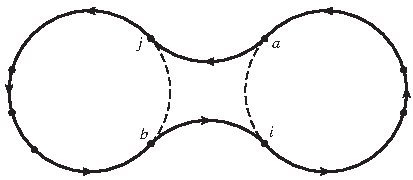
\includegraphics[width=0.567\linewidth,height=.8\textheight,keepaspectratio]{assets/p099_11.pdf}\end{center}
\begin{center}\small\textbf{8.20 Figure}\end{center}
\end{BookFloat}

Computing the product of the first three cycles in \BookInline{\tau \sigma = (i,\allowbreak j)\sigma,\allowbreak } we obtain

\begin{center}\begin{adjustbox}{max width=\linewidth}\BookInline{\displaystyle (i,\allowbreak j)(b,\allowbreak j,\allowbreak \times ,\allowbreak \times ,\allowbreak \times )(a,\allowbreak i,\allowbreak \times ,\allowbreak \times )= (a,\allowbreak j,\allowbreak \times ,\allowbreak \times ,\allowbreak \times ,\allowbreak b,\allowbreak i,\allowbreak \times ,\allowbreak \times ).}\end{adjustbox}\end{center}

The original 2 orbits have been joined to form just one in \BookInline{\tau \sigma } as symbolized in Fig. 8.20. Exercise 42 asks us to repeat the computation to show that the same thing happens if either one or both of \BookInline{i} and \BookInline{j} should be the only element of their orbit in \BookInline{\sigma.}

\noindent \textbf{Case II} Suppose \BookInline{i} and \BookInline{j} are in the same orbit of \BookInline{\sigma.} We can then write \BookInline{\sigma } as a product of disjoint cycles with the first cycle of the form

\begin{center}\begin{adjustbox}{max width=\linewidth}\BookInline{\displaystyle (a,\allowbreak i,\allowbreak \times ,\allowbreak \times ,\allowbreak \times ,\allowbreak b,\allowbreak j,\allowbreak \times ,\allowbreak \times )}\end{adjustbox}\end{center}

\end{BookBody}

% Source PDF page 100; original printed page 83
\BookSource{100}{83}
\BookNarrativetrue

\begin{BookBody}

shown symbolically by the circle in Fig. 8.20. Computing the product of the first two cycles in \BookInline{\tau \sigma = (i,\allowbreak j)\sigma,\allowbreak } we obtain

\begin{BookFloat}{08_groups_of_permutations-p100-1}
\begin{center}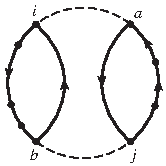
\includegraphics[width=0.228\linewidth,height=.8\textheight,keepaspectratio]{assets/p100_00.pdf}\end{center}
\begin{center}\small\textbf{8.21 Figure}\end{center}
\end{BookFloat}

\begin{center}\begin{adjustbox}{max width=\linewidth}\BookInline{\displaystyle (i,\allowbreak j)(a,\allowbreak i,\allowbreak \times ,\allowbreak \times ,\allowbreak \times ,\allowbreak b,\allowbreak j,\allowbreak \times ,\allowbreak \times )= (a,\allowbreak j,\allowbreak \times ,\allowbreak \times )(b,\allowbreak i,\allowbreak \times ,\allowbreak \times ,\allowbreak \times ).}\end{adjustbox}\end{center}

The original single orbit has been split into two as symbolized in Fig. 8.21.

We have shown that the number of orbits of \BookInline{\tau \sigma } differs from the number of orbits of \BookInline{\sigma } by 1. The identity permutation \BookInline{\iota } has \BookInline{n} orbits, because each element is the only member of its orbit. Now the number of orbits of a given permutation \BookInline{\sigma \in S_{n}} differs from \BookInline{n} by either an even or an odd number, but not both. Thus it is impossible to write

\begin{center}\begin{adjustbox}{max width=\linewidth}\BookInline{\displaystyle \sigma = \tau _{1}\tau _{2}\tau _{3}\cdots \tau _{m}\iota}\end{adjustbox}\end{center}

where the \BookInline{\tau _{k}} are transpositions in two ways, once with \BookInline{m} even and once with \BookInline{m} odd\BookInline{.}\BookEnd{\blacklozenge}

\BookLabel{8.22 Definition} A permutation of a finite set is\textbf{ even} or\textbf{ odd} according to whether it can be expressed as a product of an even number of transpositions or the product of an odd number of transpositions, respectively\BookInline{.}\BookEnd{\blacksquare}

\BookLabel{8.23 Example} The identity permutation \BookInline{\iota } in \BookInline{S_{n}} is an even permutation since we have \BookInline{\iota = (1,\allowbreak 2)(1,\allowbreak 2).} If \BookInline{n= 1} so that we cannot form this product, we define \BookInline{\iota } to be even. On the other hand, the permutation (1, 4, 5, 6) (2, 1, 5) in \BookInline{S_{6}} can be written as

\begin{center}\begin{adjustbox}{max width=\linewidth}\BookInline{\displaystyle (1,\allowbreak 4,\allowbreak 5,\allowbreak 6)(2,\allowbreak 1,\allowbreak 5)= (1,\allowbreak 6)(1,\allowbreak 5)(1,\allowbreak 4)(2,\allowbreak 5)(2,\allowbreak 1)}\end{adjustbox}\end{center}

\noindent which has five transpositions, so this is an odd permutation. \BookEnd{\blacktriangle}

\BookTextHeading{\textbf{The Alternating Groups}  }

\noindent We claim that for \BookInline{n\geq 2,\allowbreak } the number of even permutations in \BookInline{S_{n}} is the same as the number of odd permutations; that is\BookInline{,\allowbreak S_{n}} is split equally and both numbers are \BookInline{(n!)/2.} To show this, let \BookInline{A_{n}} be the set of even permutations in \BookInline{S_{n}} and let \BookInline{B_{n}} be the set of odd permutations for \BookInline{n\geq 2.} We proceed to define a one-to-one function from \BookInline{A_{n}} onto \BookInline{B_{n}.} This is exactly what is needed to show that \BookInline{A_{n}} and \BookInline{B_{n}} have the same number of elements.

Let \BookInline{\tau } be any fixed transposition in \BookInline{S_{n};} it exists since \BookInline{n\geq 2.} We may as well suppose that \BookInline{\tau = (1,\allowbreak 2).} We define a function

\begin{center}\begin{adjustbox}{max width=\linewidth}\BookInline{\displaystyle \lambda _{\tau }:A_{n}\to B_{n}}\end{adjustbox}\end{center}

\noindent by

\begin{center}\begin{adjustbox}{max width=\linewidth}\BookInline{\displaystyle \lambda _{\tau }(\sigma )= \tau \sigma ,\allowbreak }\end{adjustbox}\end{center}

\noindent that is\BookInline{,\allowbreak \sigma \in A_{n}} is mapped into \BookInline{(1,\allowbreak 2)\sigma } by \BookInline{\lambda _{\tau }.} Observe that since \BookInline{\sigma } is even, the permutation \BookInline{(1,\allowbreak 2)\sigma } can be expressed as a product of a \BookInline{(1+ } even number), or odd number, of transpositions, so \BookInline{(1,\allowbreak 2)\sigma } is indeed in \BookInline{B_{n}.} If for \BookInline{\sigma } and \BookInline{\mu } in \BookInline{A_{n}} it is true that \BookInline{\lambda _{\tau }(\sigma )= \lambda _{\tau }(\mu ),\allowbreak } then

\begin{center}\begin{adjustbox}{max width=\linewidth}\BookInline{\displaystyle (1,\allowbreak 2)\sigma = (1,\allowbreak 2)\mu ,\allowbreak }\end{adjustbox}\end{center}

\noindent and since \BookInline{S_{n}} is a group, we have \BookInline{\sigma = \mu.} Thus \BookInline{\lambda _{\tau }} is a one-to-one function. Finally,

\begin{center}\begin{adjustbox}{max width=\linewidth}\BookInline{\displaystyle \tau = (1,\allowbreak 2)= \tau ^{- 1},\allowbreak }\end{adjustbox}\end{center}

\noindent so if \BookInline{\rho \in B_{n},\allowbreak } then

\begin{center}\begin{adjustbox}{max width=\linewidth}\BookInline{\displaystyle \tau ^{- 1}\rho \in A_{n},\allowbreak }\end{adjustbox}\end{center}

\end{BookBody}

% Source PDF page 101; original printed page 84
\BookSource{101}{84}
\BookNarrativetrue

\begin{BookBody}

\noindent and

\begin{center}\begin{adjustbox}{max width=\linewidth}\BookInline{\displaystyle \lambda _{\tau }(\tau ^{- 1}\rho )= \tau (\tau ^{- 1}\rho )= \rho .}\end{adjustbox}\end{center}

\noindent Thus \BookInline{\lambda _{\tau }} maps onto \BookInline{B_{n}.} Hence the number of elements in \BookInline{A_{n}} is the same as the number in \BookInline{B_{n}} since there is a one-to-one correspondence between the elements of the sets.

Note that the product of two even permutations is again even. Also since \BookInline{n\geq 2,\allowbreak S_{n}} has the transposition (1, 2) and \BookInline{\iota = (1,\allowbreak 2)(1,\allowbreak 2)} is an even permutation. Finally, note that if \BookInline{\sigma } is expressed as a product of transpositions, the product of the same transpositions taken in just the opposite order is \BookInline{\sigma ^{- 1}.} Thus if \BookInline{\sigma } is an even permutation\BookInline{,\allowbreak \sigma ^{- 1}} must also be even. Referring to Theorem 5.12, we see that we have proved the following statement.

\BookLabel{8.24 Theorem} If \BookInline{n\geq 2,\allowbreak } then the collection of all even permutations of \BookInline{\{1,\allowbreak 2,\allowbreak 3,\allowbreak \cdots,\allowbreak n\}} forms a subgroup of order \BookInline{n!/2} of the symmetric group \BookInline{S_{n}.}

We can define a function called the\textbf{ sign of a permutation}, sgn \BookInline{:S_{n}\to \{1,\allowbreak - 1\}} by the formula

\begin{center}\begin{adjustbox}{max width=\linewidth}\BookInline{\displaystyle \operatorname { s g n } ( \sigma ) = \left\{ { \begin{array} { r l } { 1 \quad { \mathrm { i f ~ } } \sigma { \mathrm { ~ i s ~ e v e n } } } \\ { - 1 \quad { \mathrm { i f ~ } } \sigma { \mathrm { ~ i s ~ o d d } } . } \end{array} } \right.}\end{adjustbox}\end{center}

\noindent Thinking of \BookInline{\{1,\allowbreak - 1\}} as a group under multiplication, it is easy to see that sgn is a homomorphism. Since 1 is the identity in the group \BookInline{\{1,\allowbreak - 1\},\allowbreak } Ker(sgn\BookInline{)\; = } sgn\BookInline{- 1[\{1\}]} is a subgroup of \BookInline{S_{n}} consisting of all the even permutations. The homomorphism sgn is used in the standard way of defining the determinant of a square matrix. Exercise 52 asks you to prove some of the standard facts about determinants using this definition.

\BookLabel{8.25 Definition} The subgroup of \BookInline{S_{n}} consisting of the even permutations of \BookInline{n} letters is the\textbf{ alternating} \textbf{group} \BookInline{A_{n}} \textbf{on} \BookInline{n} \textbf{letters}\BookInline{.}\BookEnd{\blacksquare}

\noindent Both \BookInline{S_{n}} and \BookInline{A_{n}} are very important groups. Cayley’s theorem shows that every finite group \BookInline{G} is structurally identical to some subgroup of \BookInline{S_{n}} for \BookInline{n= |G|.} It can be shown that there are no formulas involving just radicals for solution of polynomial equations of degree \BookInline{n} for \BookInline{n\geq 5.} This fact is actually due to the structure of \BookInline{A_{n},\allowbreak } surprising as that may seem!

\end{BookBody}

\BookNarrativefalse

\begin{BookBody}

\BookExerciseTitle{8}

\BookTextHeading{\textbf{Computations}}

\noindent In Exercises 1 through 10 determine whether the given map is a group homomorphism. [Hint: To verify that a map is a homomorphism, you must check the homomorphism property. To check that a map is not a homomorphism you could either find \BookInline{a} and \BookInline{b} such that \BookInline{\phi (ab)\neq \phi (a)\phi (b),\allowbreak } or else you could determine that any of the properties in Theorem 8.5 fail.]

\BookExercise{1.}{Let \BookInline{\phi:\mathbb{Z}_{10}\to \mathbb{Z}_{2}} be given by \BookInline{\phi (x)= } the remainder when \BookInline{x} is divided by 2.}

\BookExercise{2.}{Let \BookInline{\phi:\mathbb{Z}_{9}\to \mathbb{Z}_{2}} be given by \BookInline{\phi (x)= } the remainder when \BookInline{x} is divided by 2.}

\BookExercise{3.}{Let \BookInline{\phi:\mathbb{Q}^{\ast }\to \mathbb{Q}^{\ast }} be given by \BookInline{\phi (x)= |x|.}}

\BookExercise{4.}{Let \BookInline{\phi:\mathbb{R}\to \mathbb{R}^{+ }} be given by \BookInline{\phi (x)= 2^{x}.}}

\BookExercise{5.}{Let \BookInline{\phi:D_{4}\to \mathbb{Z}_{4}} be given by \BookInline{\phi (\rho ^{i})= \phi (\mu \rho ^{i})= i} for \BookInline{0\leq i\leq 3.}}

\end{BookBody}

% Source PDF page 102; original printed page 85
\BookSource{102}{85}
\BookNarrativefalse

\begin{BookBody}

\BookExercise{6.}{Let \BookInline{F} be the additive group of all functions mapping \BookInline{\mathbb{R}} to \BookInline{\mathbb{R}.} Let \BookInline{\phi:F\to F} be given by \BookInline{\phi (f)= g} where \BookInline{g(x)= f(x)+ x.}}

\BookExercise{7.}{Let \BookInline{F} be as in Exercise 6 and \BookInline{\phi:F\to F} be defined by \BookInline{\phi (f)= 5f.}}

\BookExercise{8.}{\BookInline{\int _{0}^{1}g(x)dx.} Let \BookInline{F} be the additive group of all continuous functions mapping \BookInline{\mathbb{R}} to \BookInline{\mathbb{R}.} Let \BookInline{\phi:F\to \mathbb{R}} be defined by \BookInline{\phi (g)= }}

\BookExercise{9.}{Let \BookInline{M_{n}} be the additive group of \BookInline{n\times n} matrices with real entries. Let \BookInline{\phi:M_{n}\to \mathbb{R}} be given by \BookInline{\phi (A)= } det\BookInline{(A),\allowbreak } the determinant of \BookInline{A.}}

\BookExercise{10.}{Let \BookInline{M_{n}} be as in Exercise 9 and \BookInline{\phi:M_{n}\to \mathbb{R}} be defined by \BookInline{\phi (A)= } tr\BookInline{(A)} where tr\BookInline{(A)} is the trace of \BookInline{A,\allowbreak } which is the sum of the entries on the diagonal.}

\noindent In Exercises 11 through 16, compute the kernel for the given homomorphism \BookInline{\phi.}

\BookExercise{11.}{\BookInline{\phi:\mathbb{Z}\to \mathbb{Z}_{8}} such that \BookInline{\phi (1)= 6.}}

\BookExercise{12.}{\BookInline{\phi:\mathbb{Z}\to \mathbb{Z}} such that \BookInline{\phi (1)= 12.}}

\BookExercise{13.}{\BookInline{\phi:\mathbb{Z}\times \mathbb{Z}\to \mathbb{Z}} where \BookInline{\phi (1,\allowbreak 0)= 3} and \BookInline{\phi (0,\allowbreak 1)= - 5.}}

\BookExercise{14.}{\BookInline{\phi:\mathbb{Z}\times \mathbb{Z}\to \mathbb{Z}} where \BookInline{\phi (1,\allowbreak 0)= 6} and \BookInline{\phi (0,\allowbreak 1)= 9.}}

\BookExercise{15.}{\BookInline{\phi:\mathbb{Z}\times \mathbb{Z}\to \mathbb{Z}\times \mathbb{Z}} where \BookInline{\phi (1,\allowbreak 0)= (2,\allowbreak 5)} and \BookInline{\phi (0,\allowbreak 1)= (- 3,\allowbreak 2).}}

\BookExercise{16.}{Let \BookInline{D} be the additive group of all differentiable functions mapping \BookInline{\mathbb{R}} to \BookInline{\mathbb{R}} and \BookInline{F} the additive group of all functions from \BookInline{\mathbb{R}} to \BookInline{\mathbb{R}.\phi:D\to F} is given by \BookInline{\phi (f)= f^{\prime },\allowbreak } the derivative of \BookInline{f.}}

\noindent In Exercises 17 through 22, find all orbits of the given permutation.

\begin{enumerate}[start=17,label=\textbf{\arabic*.},leftmargin=2.5em,labelwidth=2em,labelsep=.5em,align=left]
\item \BookInline{\begin{pmatrix}1&2&3&4&5&6\\5&1&3&6&2&4\end{pmatrix}}
\item \BookInline{\begin{pmatrix}1&2&3&4&5&6&7&8\\5&6&2&4&8&3&1&7\end{pmatrix}}
\item \BookInline{\begin{pmatrix}1&2&3&4&5&6&7&8\\2&3&5&1&4&6&8&7\end{pmatrix}}
\item \BookInline{\sigma:\mathbb{Z}\to\mathbb{Z}} where \BookInline{\sigma(n)=n+1}.
\item \BookInline{\sigma:\mathbb{Z}\to\mathbb{Z}} where \BookInline{\sigma(n)=n+2}.
\item \BookInline{\sigma:\mathbb{Z}\to\mathbb{Z}} where \BookInline{\sigma(n)=n-3}.
\end{enumerate}
In Exercises 23 through 25, express the permutation of \BookInline{\{1,2,3,4,5,6,7,8\}} as a product of disjoint cycles, and then as a product of transpositions.
\begin{enumerate}[start=23,label=\textbf{\arabic*.},leftmargin=2.5em,labelwidth=2em,labelsep=.5em,align=left]
\item \BookInline{\begin{pmatrix}1&2&3&4&5&6&7&8\\8&2&6&3&7&4&5&1\end{pmatrix}}
\item \BookInline{\begin{pmatrix}1&2&3&4&5&6&7&8\\3&6&4&1&8&2&5&7\end{pmatrix}}
\item \BookInline{\begin{pmatrix}1&2&3&4&5&6&7&8\\5&3&2&8&4&7&6&1\end{pmatrix}}
\end{enumerate}

\BookExercise{26.}{Figure 8.26 shows a Cayley digraph for the alternating group \BookInline{A_{4}} using the generating set \BookInline{S= \{(1,\allowbreak 2,\allowbreak 3),\allowbreak } \BookInline{(1,\allowbreak 2)(3,\allowbreak 4)\}.} Continue labeling the other nine vertices with the elements of \BookInline{A_{4},\allowbreak } expressed as a product of disjoint cycles.}

\BookTextHeading{\textbf{Concepts}}

\noindent In Exercises 27 through 29, correct the definition of the italicized term without reference to the text, if correction is needed, so that it is in a form acceptable for publication.

\BookExercise{27.}{For a permutation \BookInline{\sigma } of a set \BookInline{A,\allowbreak } an\textit{ orbit} of \BookInline{\sigma } is a nonempty minimal subset of \BookInline{A} that is mapped onto itself by \BookInline{\sigma.}}

\BookExercise{28.}{The left regular representation of a group \BookInline{G} is the map of \BookInline{G} into \BookInline{S_{G}} whose value at \BookInline{g\in G} is the permutation of \BookInline{G} that carries each \BookInline{x\in G} into \BookInline{gx.}}

\BookExercise{29.}{The\textit{ alternating group} is the group of all even permutations.}

\end{BookBody}

% Source PDF page 103; original printed page 86
\BookSource{103}{86}
\BookNarrativefalse

\begin{BookBody}

\begin{BookFloat}{08_groups_of_permutations-p103-0}
\begin{center}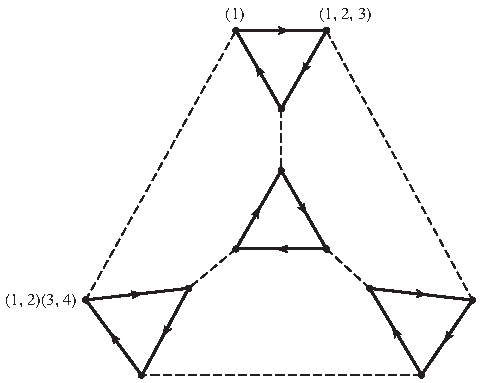
\includegraphics[width=0.658\linewidth,height=.8\textheight,keepaspectratio]{assets/p103_00.pdf}\end{center}
\begin{center}\small\textbf{8.26 Figure}\end{center}
\end{BookFloat}

\BookExercise{30.}{Before the proof of Cayley’s Theorem, it is shown that \BookInline{\lambda _{x}} is one-to-one. In the proof, one-to-one is shown again. Is it necessary to show one-to-one twice? Explain.}

\BookExercise{31.}{Determine whether each of the following is true or false.}

\BookExercise{a.}{Every permutation is a cycle.}

\BookExercise{b.}{Every cycle is a permutation.}

\BookExercise{c.}{The definition of even and odd permutations could have been given equally well before Theorem 8.19.}

\BookExercise{d.}{Every nontrivial subgroup \BookInline{H} of \BookInline{S_{9}} containing some odd permutation contains a transposition.}

\BookExercise{e.}{\textbf{e}\BookInline{.A_{5}} has 120 elements.}

\BookExercise{f.}{\textbf{f}\BookInline{.S_{n}} is not cyclic for any \BookInline{n\geq 1.}}

\BookExercise{g.}{\textbf{g}\BookInline{.A_{3}} is a commutative group.}

\BookExercise{h.}{\textbf{h}\BookInline{.S_{7}} is isomorphic to the subgroup of all those elements of \BookInline{S_{8}} that leave the number 8 fixed.}

\BookExercise{i.}{\textbf{i}\BookInline{.S_{7}} is isomorphic to the subgroup of all those elements of \BookInline{S_{8}} that leave the number 5 fixed.}

\BookExercise{j.}{The odd permutations in \BookInline{S_{8}} form a subgroup of \BookInline{S_{8}.}}

\BookExercise{k.}{Every group \BookInline{G} is isomorphic with a subgroup of \BookInline{S_{G}.}}

\BookExercise{32.}{The dihedral group is defined to be permutations with certain properties. Use the usual notation involving \BookInline{\mu } and \BookInline{\rho } for elements in \BookInline{D_{n}.}}

\BookExercise{a.}{Identify which elements in \BookInline{D_{3}} are even. Do the even elements form a cyclic group?}

\BookExercise{b.}{Identify which of elements of \BookInline{D_{4}} are even. Do the even elements form a cyclic group?}

\BookExercise{c.}{For which values of \BookInline{n} do the even permutations of \BookInline{D_{n}} form a cyclic group?}

\BookLabel{\textit{Proof}} \textbf{ Synopsis}

\BookExercise{33.}{Give a two-sentence synopsis of the proof of Cayley’s Theorem.}

\BookExercise{34.}{Give a two-sentence synopsis of the proof of Theorem 8.19.}

\BookTextHeading{\textbf{Theory}}

\BookExercise{35.}{Suppose that \BookInline{\phi:G\to G^{\prime }} is a group homomorphism and \BookInline{a\in } Ker\BookInline{\phi.} Show that for any \BookInline{g\in G,\allowbreak gag^{- 1}\in } Ker\BookInline{\phi.}}

\BookExercise{36.}{Prove that a homomorphism \BookInline{\phi:G\to G^{\prime }} is one-to-one if and only if Ker\BookInline{(\phi )} is the trivial subgroup of \BookInline{G.}}

\BookExercise{37.}{Let \BookInline{\phi:G\to G^{\prime }} be a group homomorphism. Show that \BookInline{\phi (a)= \phi (b)} if and only if \BookInline{a^{- 1}b\in } Ker\BookInline{\phi.}}

\BookExercise{38.}{Use Exercise 37 to prove that if \BookInline{\phi:G\to G^{\prime }} is a group homomorphism mapping onto \BookInline{G^{\prime }} and \BookInline{G} is a finite group, then for any \BookInline{b,\allowbreak c\in G^{\prime },\allowbreak |\phi ^{- 1}[\{b\}]|= |\phi ^{- 1}[\{c\}]|.} Conclude that if \BookInline{|G|} is a prime number, then either \BookInline{\phi } is an isomorphism or else \BookInline{G^{\prime }} is the trivial group.}

\end{BookBody}

% Source PDF page 104; original printed page 87
\BookSource{104}{87}
\BookNarrativetrue

\begin{BookBody}

\BookExercise{39.}{Show that if \BookInline{\phi:G\to G^{\prime }} and \BookInline{\gamma:G^{\prime }\to G^{\prime \prime }} are group homomorphisms, then \BookInline{\gamma \circ \phi:G\to G^{\prime \prime }} is also a group homomorphism.}

\BookExercise{40.}{Let \BookInline{\phi:G\to G^{\prime }} be a group homomorphism. Show that \BookInline{\phi [G]} is abelian if and only if \BookInline{xyx^{- 1}y^{- 1}\in } Ker\BookInline{(\phi )} for all \BookInline{x,\allowbreak y\in G.}}

\BookExercise{41.}{Prove the following about \BookInline{S_{n}} if \BookInline{n\geq 3.}}

\BookExercise{a.}{Every permutation in \BookInline{S_{n}} can be written as a product of at most \BookInline{n- 1} transpositions.}

\BookExercise{b.}{Every permutation in \BookInline{S_{n}} that is not a cycle can be written as a product of at most \BookInline{n- 2} transpositions.}

\BookExercise{c.}{Every odd permutation in \BookInline{S_{n}} can be written as a product of \BookInline{2n+ 3} transpositions, and every even permutation as a product of \BookInline{2n+ 8} transpositions.}

\BookExercise{42.}{\textbf{. a} Draw a figure like Fig. 8.20 to illustrate that if \BookInline{i} and \BookInline{j} are in different orbits of \BookInline{\sigma } and \BookInline{\sigma (i)= i,\allowbreak } then the number of orbits of \BookInline{(i,\allowbreak j)\sigma } is one less than the number of orbits of \BookInline{\sigma.}}

\BookExercise{b.}{Repeat part (a) if \BookInline{\sigma (j)= j} also.}

\BookExercise{43.}{Show that for every subgroup \BookInline{H} of \BookInline{S_{n}} for \BookInline{n\geq 2,\allowbreak } either all the permutations in \BookInline{H} are even or exactly half of them are even.}

\BookExercise{44.}{Let \BookInline{\sigma } be a permutation of a set \BookInline{A.} We shall say “\BookInline{\sigma } \textbf{moves} \BookInline{a\in A}” if \BookInline{\sigma (a)\neq a.} If \BookInline{A} is a finite set, how many elements are moved by a cycle \BookInline{\sigma \in S_{A}} of length \BookInline{n}?}

\BookExercise{45.}{Let \BookInline{A} be an infinite set. Let \BookInline{H} be the set of all \BookInline{\sigma \in S_{A}} such that the number of elements moved by \BookInline{\sigma (}see Exercise 44) is finite. Show that \BookInline{H} is a subgroup of \BookInline{S_{A}.}}

\BookExercise{46.}{Let \BookInline{A} be an infinite set. Let \BookInline{K} be the set of all \BookInline{\sigma \in S_{A}} that move (see Exercise 44) at most 50 elements of \BookInline{A.} Is \BookInline{K} a subgroup of \BookInline{S_{A}}? Why?}

\BookExercise{47.}{Consider \BookInline{S_{n}} for a fixed \BookInline{n\geq 2} and let \BookInline{\sigma } be a fixed odd permutation. Show that every odd permutation in \BookInline{S_{n}} is a product of \BookInline{\sigma } and some permutation in \BookInline{A_{n}.}}

\BookExercise{48.}{Show that if \BookInline{\sigma } is a cycle of odd length, then \BookInline{\sigma ^{2}} is a cycle.}

\BookExercise{49.}{Following the line of thought opened by Exercise 48, complete the following with a condition involving \BookInline{n} and \BookInline{r} so that the resulting statement is a theorem:}

\noindent If \BookInline{\sigma } is a cycle of length \BookInline{n,\allowbreak } then \BookInline{\sigma ^{r}} is also a cycle if and only if \BookInline{...}

\BookExercise{50.}{Show that \BookInline{S_{n}} is generated by \BookInline{\{(1,\allowbreak 2),\allowbreak (1,\allowbreak 2,\allowbreak 3,\allowbreak \cdots,\allowbreak n)\}.[}\textit{Hint:} Show that as \BookInline{r} varies\BookInline{,\allowbreak (1,\allowbreak 2,\allowbreak 3,\allowbreak \cdots,\allowbreak n)^{r}(1,\allowbreak 2)} \BookInline{(1,\allowbreak 2,\allowbreak 3,\allowbreak \cdots,\allowbreak n)^{n- r}} gives all the transpositions \BookInline{(1,\allowbreak 2),\allowbreak (2,\allowbreak 3),\allowbreak (3,\allowbreak 4),\allowbreak \cdots,\allowbreak (n- 1,\allowbreak n),\allowbreak (n,\allowbreak 1).} Then show that any transposition is a product of some of these transpositions and use Theorem 8.15.]}

\BookExercise{51.}{Let \BookInline{\sigma \in S_{n}} and define a relation on \BookInline{\{1,\allowbreak 2,\allowbreak 3,\allowbreak...,\allowbreak n\}} by \BookInline{i\sim j} if and only if \BookInline{j= \sigma ^{k}(i)} for some \BookInline{k\in \mathbb{Z}.}}

\BookExercise{1.}{Prove that \BookInline{\sim } is an equivalence relation.}

\BookExercise{2.}{Prove that for any \BookInline{1\leq i\leq n,\allowbreak } the equivalence class of \BookInline{i} is the orbit of \BookInline{i.}}

\BookExercise{52.}{The usual definition for the determinant of an \BookInline{n\times n} matrix \BookInline{A= (a_{i,\allowbreak j})} is}

\begin{center}\begin{adjustbox}{max width=\linewidth}\BookInline{\displaystyle \;\text{det}\;(A)= _{\sigma }\sum _{\in S_{n}}\;\text{sgn}\;(\sigma )a_{1,\allowbreak \sigma (1)}a_{2,\allowbreak \sigma (2)}a_{3,\allowbreak \sigma (3)}\cdots a_{n,\allowbreak \sigma (n)}}\end{adjustbox}\end{center}

\noindent where sgn\BookInline{(\sigma )} is the sign of \BookInline{\sigma.} Using this definition, prove the following properties of determinants.

\BookExercise{a.}{If a row of matrix \BookInline{A} has all zero entries, then det\BookInline{(A)= 0.}}

\BookExercise{b.}{If two different rows of \BookInline{A} are switched to obtain \BookInline{B,\allowbreak } then det\BookInline{(B)= - } det\BookInline{(A).}}

\BookExercise{c.}{If \BookInline{r} times one row of \BookInline{A} is added to another row of \BookInline{A} to obtain a matrix \BookInline{B,\allowbreak } then det\BookInline{(A)= } det\BookInline{(B)}}

\BookExercise{d.}{If a row of \BookInline{A} is multiplied by \BookInline{r} to obtain the matrix \BookInline{B,\allowbreak } then det\BookInline{(B)= r} det\BookInline{(A).}}

\BookExercise{53.}{Prove that any finite group \BookInline{G} is isomorphic with a subgroup of GL\BookInline{(n,\allowbreak \mathbb{R})} for some \BookInline{n.[}Hint: For each \BookInline{\sigma \in S_{n},\allowbreak } find a matrix in GL\BookInline{(n,\allowbreak \mathbb{R})} that sends each basis vector \BookInline{e_{i}} to \BookInline{e_{\sigma (i)}.} Use this to show that \BookInline{S_{n}} is isomorphic with a subgroup of GL\BookInline{(n,\allowbreak \mathbb{R}).]}}

\BookExercise{54.}{Prove Cayley’s Theorem using the right regular representation rather than the left regular representation.}

\BookExercise{55.}{Let \BookInline{\sigma \in S_{n}.} An inversion is a pair \BookInline{(i,\allowbreak j)} such that \BookInline{i<j} and \BookInline{\sigma (i)>\sigma (j).} Prove Theorem 8.19 by showing that multiplying a permutation by a transposition changes the number of inversions by an odd number.}

\end{BookBody}

% Continuation on source PDF page 105, preceding Section 9
\BookNarrativefalse

\begin{BookBody}

\BookExercise{56.}{The sixteen puzzle consists of 15 tiles numbered 1 through 15 arranged in a four-by-four grid with one position left blank. A move is sliding a tile adjacent to the blank position into the blank position. The goal is to arrange the numbers in order by a sequence of moves. Is it possible to start with the configuration pictured in Figure 8.27(a) and solve the puzzle as indicated in Figure 8.27(b)? Prove your answer by finding a sequence of moves to solve the puzzle or by proving that it is impossible to solve.}

\begin{BookFloat}{08_groups_of_permutations-p105-1}
\begin{center}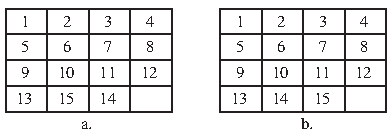
\includegraphics[width=0.536\linewidth,height=.8\textheight,keepaspectratio]{assets/p105_01.pdf}\end{center}
\begin{center}\small\textbf{8.27 Figure}\end{center}
\end{BookFloat}

\end{BookBody}
\ifdefined\BookMaster\let\BookFinish\relax\else\def\BookFinish{\end{document}}\fi\BookFinish

\clearpage
% !TeX program = xelatex
\ifdefined\BookMaster\else
\documentclass[11pt,oneside]{article}
% !TeX program = xelatex
\usepackage[b5paper,left=22mm,right=22mm,top=20mm,bottom=22mm,footskip=11mm]{geometry}
\usepackage{fontspec}
\setmainfont{TeX Gyre Termes}
\setsansfont{TeX Gyre Heros}
\usepackage{amsmath,amssymb,mathtools,amsthm}
\renewcommand{\cdots}{\mathinner{\cdotp\cdotp\cdotp}}
\usepackage{graphicx,adjustbox,array,booktabs,longtable,multirow,enumitem,changepage,needspace}
\usepackage[table]{xcolor}
\usepackage{fancyhdr}
\raggedbottom
\interfootnotelinepenalty=10000
\newcommand{\BookFootnote}[2]{\begingroup\renewcommand{\thefootnote}{\fnsymbol{footnote}}\footnote[#1]{#2}\endgroup}
\newcommand{\BookFootnoteMark}[1]{\begingroup\renewcommand{\thefootnote}{\fnsymbol{footnote}}\footnotemark[#1]\endgroup}
\newcommand{\BookFootnoteText}[2]{\begingroup\renewcommand{\thefootnote}{\fnsymbol{footnote}}\footnotetext[#1]{#2}\endgroup}
\newenvironment{BookFloat}[1]{\par\addvspace{.6\baselineskip}\noindent\def\BookFloatID{#1}\begin{minipage}{\linewidth}\phantomsection\label{bookfloat:#1:start}}{\phantomsection\label{bookfloat:\BookFloatID:end}\end{minipage}\par\addvspace{.6\baselineskip}}

\usepackage[unicode,hidelinks]{hyperref}
\pagestyle{fancy}
\fancyhf{}
\newcommand{\BookFooter}{}
\fancyfoot[L]{\parbox[b]{\dimexpr\textwidth-15mm}{\footnotesize\BookFooter}}
\fancyfoot[R]{\footnotesize\thepage}
\renewcommand{\headrulewidth}{0pt}
\renewcommand{\footrulewidth}{0pt}
\setlength{\parindent}{0pt}
\setlength{\parskip}{0.2em}
\setlength{\emergencystretch}{3em}
\setlist{nosep,leftmargin=1.7em,labelsep=.65em}
\newif\ifBookNarrative
\BookNarrativetrue
\newenvironment{BookBody}{\setlength{\parindent}{0pt}}{}
\newcommand{\BookStatement}[1]{\par\addvspace{.6\baselineskip}\noindent #1\enspace\ignorespaces}
\newcommand{\BookLabel}[1]{\par\addvspace{.6\baselineskip}\needspace{3\baselineskip}\noindent\textbf{#1}\quad\ignorespaces}
\newcommand{\BookHeading}[1]{\par\addvspace{\baselineskip}\needspace{4\baselineskip}\noindent{\large\bfseries #1}\par\medskip}
\newcommand{\BookSubheading}[1]{\par\addvspace{.7\baselineskip}\needspace{3\baselineskip}\noindent{\bfseries #1}\par\smallskip}
\newcommand{\BookTextHeading}[1]{\par\addvspace{.7\baselineskip}\needspace{3\baselineskip}\noindent #1\par\smallskip}
\newcommand{\BookSectionTitle}[2]{\par\addvspace{1.2\baselineskip}\needspace{5\baselineskip}\noindent\colorbox{gray!25}{\sffamily\bfseries\small SECTION #1}\quad{\large\bfseries #2}\par\medskip}
\newcommand{\BookExerciseTitle}[1]{\par\addvspace{\baselineskip}\needspace{4\baselineskip}\noindent{\color{gray}\rule{1.5mm}{1.5mm}}\enspace{\large\bfseries Exercises #1}\par\medskip}
\newcommand{\BookBullet}[1]{\begin{list}{\textbullet}{\setlength{\leftmargin}{1.7em}\setlength{\labelwidth}{1em}\setlength{\labelsep}{.7em}\setlength{\topsep}{0pt}\setlength{\parsep}{0pt}\setlength{\itemsep}{0pt}}\item #1\end{list}}
\newcommand{\BookExercise}[2]{\begin{list}{\textbf{#1}}{\setlength{\leftmargin}{2.2em}\setlength{\labelwidth}{1.5em}\setlength{\labelsep}{.7em}\setlength{\topsep}{.15em}\setlength{\parsep}{0pt}\setlength{\itemsep}{0pt}}\item #2\end{list}}
\newcommand{\BookEnd}[1]{\unskip\nobreak\hfill\ensuremath{#1}}
\newcommand{\BookSource}[2]{\phantomsection\label{sourcepage:#1}} % Source-page anchors, retained through reflow.
\usepackage{multicol}
\usepackage{tikz}
\newcommand{\BookPartEntry}[2]{\par\noindent\makebox[17mm][l]{\bfseries Section #1}#2\par}
\newcommand{\BookPartTitle}[3]{\par\bigskip\noindent\begin{tikzpicture}\node[anchor=north west,inner sep=0pt,outer sep=0pt] (bookpart) at (0,0) {\begin{minipage}{\dimexpr\linewidth-.5pt}\hspace*{26mm}\begin{minipage}[t]{\dimexpr\linewidth-26mm}\begin{adjustbox}{max width=\linewidth}{\fontsize{20}{24}\selectfont\bfseries #2}\end{adjustbox}\par\vspace{6mm}\hrule\vspace{6mm}{\sffamily\footnotesize\setlength{\parskip}{.3em}#3}\vspace{3mm}\end{minipage}\end{minipage}};\path[shade,top color=gray!60,bottom color=white] (0,0) rectangle ([xshift=24mm]bookpart.south west);\node[anchor=north,font=\sffamily\bfseries\small] at (12mm,-2mm) {PART};\node[anchor=north,font=\sffamily\bfseries\Huge] at (12mm,-7mm) {#1};\end{tikzpicture}\par\bigskip}
\newsavebox{\BookMathBox}
\makeatletter
\newcommand{\BookInline}[1]{\leavevmode\hskip0pt\relax\begingroup\in@{\begin}{#1}\ifin@\sbox{\BookMathBox}{\(#1\)}\ifdim\wd\BookMathBox>\dimexpr\linewidth-1em\relax\resizebox{\dimexpr\linewidth-1em\relax}{!}{\usebox{\BookMathBox}}\else\(#1\)\fi\else\in@{\left}{#1}\ifin@\sbox{\BookMathBox}{\(#1\)}\ifdim\wd\BookMathBox>\dimexpr\linewidth-1em\relax\resizebox{\dimexpr\linewidth-1em\relax}{!}{\usebox{\BookMathBox}}\else\(#1\)\fi\else\(#1\)\fi\fi\endgroup\hskip0pt\relax}
\makeatother
\DeclareMathOperator{\Aut}{Aut}
\DeclareMathOperator{\End}{End}
\DeclareMathOperator{\Hom}{Hom}
\DeclareMathOperator{\GF}{GF}
\DeclareMathOperator{\irr}{irr}
\DeclareMathOperator{\lt}{lt}
\DeclareMathOperator{\lp}{lp}
\providecommand{\textcircled}[1]{\textnormal{(#1)}}

\begin{document}
\fi
\renewcommand{\BookFooter}{Section 9 Finitely Generated Abelian Groups}
\pdfbookmark[0]{Section 9 Finitely Generated Abelian Groups}{09_finitely_generated_abelian_groups}
\ifdefined\BookMaster\else\setcounter{page}{88}\fi
% Source PDF page 105; original printed page 88
\BookSource{105}{88}
\BookNarrativetrue

\begin{BookBody}

\BookSectionTitle{9}{Finitely Generated Abelian Groups}

\BookTextHeading{\textbf{Direct Products}  }

\noindent Let us take a moment to review our present stockpile of groups. Starting with finite groups, we have the cyclic group \BookInline{\mathbb{Z}_{n},\allowbreak } the symmetric group \BookInline{S_{n},\allowbreak } and the alternating group \BookInline{A_{n}} for each positive integer \BookInline{n.} We also have the dihedral groups \BookInline{D_{n}} and the Klein 4-group \BookInline{V.} Of course we know that subgroups of these groups exist. Turning to infinite groups, we have groups consisting of sets of numbers under the usual addition or multiplication, as, for example\BookInline{,\allowbreak \mathbb{Z},\allowbreak \mathbb{R},\allowbreak } and \BookInline{\mathbb{C}} under addition, and their nonzero elements under multiplication. We have the group \BookInline{U} of complex numbers of magnitude 1 under multiplication, which is isomorphic to each of the groups \BookInline{\mathbb{R}_{c}} under addition modulo \BookInline{c,\allowbreak } where \BookInline{c\in \mathbb{R}^{+ }.} We also have the group \BookInline{S_{A}} of all permutations of an infinite set \BookInline{A,\allowbreak } as well as various groups formed from matrices such as GL(n\BookInline{,\allowbreak \mathbb{R}).}

One purpose of this section is to show a way to use known groups as building blocks to form more groups. The Klein 4-group will be recovered in this way from the cyclic groups. Employing this procedure with the cyclic groups gives us a large class of abelian groups that can be shown to include all possible structure types for a finite abelian group. We start by generalizing Definition 0.4.

\BookLabel{9.1 Definition} The\textbf{ Cartesian product of sets} \BookInline{B_{1},\allowbreak B_{2},\allowbreak \cdots,\allowbreak B_{n}} is the set of all ordered \BookInline{n-}tuples \BookInline{(b_{1},\allowbreak b_{2},\allowbreak \cdots,\allowbreak b_{n}),\allowbreak } where \BookInline{b_{i}\in B_{i}} for \BookInline{i= 1,\allowbreak 2,\allowbreak \cdots,\allowbreak n.} The Cartesian product is denoted by either

\begin{center}\begin{adjustbox}{max width=\linewidth}\BookInline{\displaystyle B_{1}\times B_{2}\times \cdots \times B_{n}}\end{adjustbox}\end{center}

\noindent or by

\begin{center}\begin{adjustbox}{max width=\linewidth}\BookInline{\displaystyle \prod _{i= 1}^{n}B_{i}.}\end{adjustbox}\end{center} \BookEnd{\blacksquare}

We could also define the Cartesian product of an infinite number of sets, but the definition is considerably more sophisticated and we shall not need it.

Now let \BookInline{G_{1},\allowbreak G_{2},\allowbreak \cdots,\allowbreak G_{n}} be groups, and let us use multiplicative notation for all the group operations. Regarding the \BookInline{G_{i}} as sets, we can form \BookInline{\prod _{i= 1}^{n}G_{i}}. Let us show that we can make \BookInline{\prod _{i= 1}^{n}G_{i}} into a group by means of a binary operation of\textit{ multiplication by} \textit{components}. Note again that we are being sloppy when we use the same notation for a group as for the set of elements of the group.

\end{BookBody}

% Source PDF page 106; original printed page 89
\BookSource{106}{89}
\BookNarrativetrue

\begin{BookBody}

\BookLabel{9.2 Theorem} Let \BookInline{G_{1},\allowbreak G_{2},\allowbreak \cdots,\allowbreak G_{n}} be groups. For \BookInline{(a_{1},\allowbreak a_{2},\allowbreak \cdots,\allowbreak a_{n})} and \BookInline{(b_{1},\allowbreak b_{2},\allowbreak \cdots,\allowbreak b_{n})} in \BookInline{\prod _{i= 1}^{n}G_{i},\allowbreak } define \BookInline{(a_{1},\allowbreak a_{2},\allowbreak \cdots,\allowbreak a_{n})(b_{1},\allowbreak b_{2},\allowbreak \cdots,\allowbreak b_{n})} to be the element \BookInline{(a_{1}b_{1},\allowbreak a_{2}b_{2},\allowbreak \cdots,\allowbreak a_{n}b_{n}).} Then \BookInline{\prod _{i= 1}^{n}G_{i}} is a group, the\textbf{ direct product of the groups} \BookInline{G_{i},\allowbreak } under this binary operation.

\BookLabel{\textit{Proof}} Note that since \BookInline{a_{i}\in G_{i},\allowbreak b_{i}\in G_{i},\allowbreak } and \BookInline{G_{i}} is a group, we have \BookInline{a_{i}b_{i}\in G_{i}.} Thus the definition of the binary operation on \BookInline{\prod _{i= 1}^{n}G_{i}} given in the statement of the theorem makes sense; that is, \BookInline{\prod _{i= 1}^{n}G_{i}} is closed under the binary operation.

The associative law in \BookInline{\prod _{i= 1}^{n}G_{i}} is thrown back onto the associative law in each component as follows:

\begin{center}\begin{adjustbox}{max width=\linewidth}\BookInline{\displaystyle \begin{aligned}&(a_{1},\allowbreak a_{2},\allowbreak \cdots ,\allowbreak a_{n})[(b_{1},\allowbreak b_{2},\allowbreak \cdots ,\allowbreak b_{n})(c_{1},\allowbreak c_{2},\allowbreak \cdots ,\allowbreak c_{n})] \\ &= (a_{1},\allowbreak a_{2},\allowbreak \cdots ,\allowbreak a_{n})(b_{1}c_{1},\allowbreak b_{2}c_{2},\allowbreak \cdots ,\allowbreak b_{n}c_{n}) \\ &= (a_{1}(b_{1}c_{1}),\allowbreak a_{2}(b_{2}c_{2}),\allowbreak \cdots ,\allowbreak a_{n}(b_{n}c_{n})) \\ &= ((a_{1}b_{1})c_{1},\allowbreak (a_{2}b_{2})c_{2},\allowbreak \cdots ,\allowbreak (a_{n}b_{n})c_{n}) \\ &= (a_{1}b_{1},\allowbreak a_{2}b_{2},\allowbreak \cdots ,\allowbreak a_{n}b_{n})(c_{1},\allowbreak c_{2},\allowbreak \cdots ,\allowbreak c_{n}) \\ &= [(a_{1},\allowbreak a_{2},\allowbreak \cdots ,\allowbreak a_{n})(b_{1},\allowbreak b_{2},\allowbreak \cdots ,\allowbreak b_{n})](c_{1},\allowbreak c_{2},\allowbreak \cdots ,\allowbreak c_{n}).\end{aligned}}\end{adjustbox}\end{center}

\noindent If \BookInline{e_{i}} is the identity element in \BookInline{G_{i},\allowbreak } then clearly, with multiplication by components, \BookInline{(e_{1},\allowbreak e_{2},\allowbreak \cdots,\allowbreak e_{n})} is an identity in \BookInline{\prod _{i= 1}^{n}G_{i}}. Finally, an inverse of \BookInline{(a_{1},\allowbreak a_{2},\allowbreak \cdots,\allowbreak a_{n})} is \BookInline{(a_{1}^{- 1},\allowbreak a_{2}^{- 1},\allowbreak \cdots,\allowbreak a_{n}^{- 1});} compute the product by components. Hence \BookInline{\prod _{i= 1}^{n}G_{i}} is a group. \BookEnd{\blacklozenge}

In the event that the operation of each \BookInline{G_{i}} is commutative, we sometimes use additive notation in \BookInline{\prod _{i= 1}^{n}G_{i}} and refer to \BookInline{\prod _{i= 1}^{n}G_{i}} as the\textbf{ direct sum of the groups} \BookInline{G_{i}.} The notation \BookInline{\oplus _{i= 1}^{n}G_{i}} is sometimes used in this case in place of \BookInline{\prod _{i= 1}^{n}G_{i},\allowbreak } especially with abelian groups with operation \BookInline{+.} The direct sum of abelian groups \BookInline{G_{1},\allowbreak G_{2},\allowbreak \cdots,\allowbreak G_{n}} may be written \BookInline{G_{1}\oplus G_{2}\oplus \cdots \oplus G_{n}.} We leave to Exercise 46 the proof that a direct product of abelian groups is again abelian.

It is quickly seen that if \BookInline{B_{i}} has \BookInline{r_{i}} elements for \BookInline{i= 1,\allowbreak \cdots,\allowbreak n,\allowbreak } then \BookInline{\prod _{i= 1}^{n}B_{i}} has \BookInline{r_{1}r_{2}\cdots r_{n}} elements, for in an \BookInline{n-}tuple, there are \BookInline{r_{1}} choices for the first component from \BookInline{B_{1},\allowbreak } and for each of these there are \BookInline{r_{2}} choices for the next component from \BookInline{B_{2},\allowbreak } and so on.

\BookLabel{9.3 Example} Consider the group \BookInline{\mathbb{Z}_{2}\times \mathbb{Z}_{3},\allowbreak } which has \BookInline{2\cdot 3= 6} elements, namely (0, 0), (0, 1), (0, 2), (1, 0), (1, 1), and (1, 2). We claim that \BookInline{\mathbb{Z}_{2}\times \mathbb{Z}_{3}} is cyclic. It is only necessary to find a generator. Let us try (1, 1). Here the operations in \BookInline{\mathbb{Z}_{2}} and \BookInline{\mathbb{Z}_{3}} are written additively, so we do the same in the direct product \BookInline{\mathbb{Z}_{2}\times \mathbb{Z}_{3}.}

\begin{center}\begin{adjustbox}{max width=\linewidth}\BookInline{\displaystyle \begin{aligned}(1,\allowbreak 1)&= (1,\allowbreak 1) \\ 2(1,\allowbreak 1)&= (1,\allowbreak 1)+ (1,\allowbreak 1)= (0,\allowbreak 2) \\ 3(1,\allowbreak 1)&= (1,\allowbreak 1)+ (1,\allowbreak 1)+ (1,\allowbreak 1)= (1,\allowbreak 0) \\ 4(1,\allowbreak 1)&= 3(1,\allowbreak 1)+ (1,\allowbreak 1)= (1,\allowbreak 0)+ (1,\allowbreak 1)= (0,\allowbreak 1) \\ 5(1,\allowbreak 1)&= 4(1,\allowbreak 1)+ (1,\allowbreak 1)= (0,\allowbreak 1)+ (1,\allowbreak 1)= (1,\allowbreak 2) \\ 6(1,\allowbreak 1)&= 5(1,\allowbreak 1)+ (1,\allowbreak 1)= (1,\allowbreak 2)+ (1,\allowbreak 1)= (0,\allowbreak 0)\end{aligned}}\end{adjustbox}\end{center}

\noindent Thus (1, 1) generates all of \BookInline{\mathbb{Z}_{2}\times \mathbb{Z}_{3}.} Since there is, up to isomorphism, only one cyclic group structure of a given order, we see that \BookInline{\mathbb{Z}_{2}\times \mathbb{Z}_{3}} is isomorphic to \BookInline{\mathbb{Z}_{6}.}\BookEnd{\blacktriangle}

\BookLabel{9.4 Example} Consider \BookInline{\mathbb{Z}_{3}\times \mathbb{Z}_{3}.} This is a group of nine elements. We claim that \BookInline{\mathbb{Z}_{3}\times \mathbb{Z}_{3}} is\textit{ not} cyclic. Since the addition is by components, and since in \BookInline{\mathbb{Z}_{3}} every element added to itself three times gives the identity, the same is true in \BookInline{\mathbb{Z}_{3}\times \mathbb{Z}_{3}.} Thus no element can generate the group, for a generator added to itself successively could only give the identity after nine 
% Source PDF page 107; original printed page 90
\BookSource{107}{90}
summands. We have found another group structure of order 9. A similar argument shows that \BookInline{\mathbb{Z}_{2}\times \mathbb{Z}_{2}} is not cyclic. Thus \BookInline{\mathbb{Z}_{2}\times \mathbb{Z}_{2}} must be isomorphic to the Klein 4-group\BookInline{.}\BookEnd{\blacktriangle}

\end{BookBody}

\BookNarrativetrue

\begin{BookBody}

The preceding examples illustrate the following theorem:

\BookLabel{9.5 Theorem} The group \BookInline{\mathbb{Z}_{m}\times \mathbb{Z}_{n}} is cyclic and is isomorphic to \BookInline{\mathbb{Z}_{mn}} if and only if \BookInline{m} and \BookInline{n} are relatively prime, that is, the gcd of \BookInline{m} and \BookInline{n} is 1.

\BookLabel{\textit{Proof}} Consider the cyclic subgroup of \BookInline{\mathbb{Z}_{m}\times \mathbb{Z}_{n}} generated by (1, 1) as described by Theorem 5.19. As our previous work has shown, the order of this cyclic subgroup is the smallest power of (1, 1) that gives the identity (0, 0). Here taking a power of (1, 1) in our additive notation will involve adding (1, 1) to itself repeatedly. Under addition by components, the first component \BookInline{1\in \mathbb{Z}_{m}} yields 0 only after \BookInline{m} summands\BookInline{,\allowbreak 2m} summands, and so on, and the second component \BookInline{1\in \mathbb{Z}_{n}} yields 0 only after \BookInline{n} summands\BookInline{,\allowbreak 2n} summands, and so on. For them to yield 0 simultaneously, the number of summands must be a multiple of both \BookInline{m} and \BookInline{n.} The smallest number that is a multiple of both \BookInline{m} and \BookInline{n} will be \BookInline{mn} if and only if the gcd of \BookInline{m} and \BookInline{n} is 1; in this case, (1, 1) generates a cyclic subgroup of order \BookInline{mn,\allowbreak } which is the order of the whole group. This shows that \BookInline{\mathbb{Z}_{m}\times \mathbb{Z}_{n}} is cyclic of order \BookInline{mn,\allowbreak } and hence isomorphic to \BookInline{\mathbb{Z}_{mn}} if \BookInline{m} and \BookInline{n} are relatively prime.

For the converse, suppose that the gcd of \BookInline{m} and \BookInline{n} is \BookInline{d>1.} Then \BookInline{mn/d} is divisible by both \BookInline{m} and \BookInline{n.} Consequently, for any \BookInline{(r,\allowbreak s)} in \BookInline{\mathbb{Z}_{m}\times \mathbb{Z}_{n},\allowbreak } we have

\begin{center}\begin{adjustbox}{max width=\linewidth}\BookInline{\displaystyle \underline { { ( r ,\allowbreak  s ) + ( r ,\allowbreak  s ) } } + \dots + \underline { { ( r ,\allowbreak  s ) } } = ( 0 ,\allowbreak  0 ) .}\end{adjustbox}\end{center}

\BookInline{mn/d} summands

Hence no element \BookInline{(r,\allowbreak s)} in \BookInline{\mathbb{Z}_{m}\times \mathbb{Z}_{n}} can generate the entire group, so \BookInline{\mathbb{Z}_{m}\times \mathbb{Z}_{n}} is not cyclic and therefore not isomorphic to \BookInline{\mathbb{Z}_{mn}.}\BookEnd{\blacklozenge}

This theorem can be extended to a product of more than two factors by similar arguments. We state this as a corollary without going through the details of the proof.

\BookLabel{9.6 Corollary} The group \BookInline{\prod _{i= 1}^{n}\mathbb{Z}_{m_{i}}} is cyclic and isomorphic to \BookInline{\mathbb{Z}_{m_{1}m_{2}\cdots m_{n}}} if and only if the numbers \BookInline{m_{i}} for \BookInline{i= 1,\allowbreak \cdots,\allowbreak n} are such that the gcd of any two of them is 1.

\BookLabel{9.7 Example} The preceding corollary shows that if \BookInline{n} is written as a product of powers of distinct prime numbers, as in

\begin{center}\begin{adjustbox}{max width=\linewidth}\BookInline{\displaystyle n= (p_{1})^{n_{1}}(p_{2})^{n_{2}}\cdots (p_{r})^{n_{r}},\allowbreak }\end{adjustbox}\end{center}

\noindent then \BookInline{\mathbb{Z}_{n}} is isomorphic to

\begin{center}\begin{adjustbox}{max width=\linewidth}\BookInline{\displaystyle \mathbb{Z}_{(p_{1})^{1}}^{n}\times \mathbb{Z}_{(p_{2})^{2}}^{n}\times \cdots \times \mathbb{Z}_{(p_{r})}nr.}\end{adjustbox}\end{center}

In particular\BookInline{,\allowbreak \mathbb{Z}_{72}} is isomorphic to \BookInline{\mathbb{Z}_{8}\times \mathbb{Z}_{9}.} \BookEnd{\blacktriangle}

We remark that changing the order of the factors in a direct product yields a group isomorphic to the original one. The names of elements have simply been changed via a permutation of the components in the \BookInline{n-}tuples.

Exercise 57 of Section 6 asked you to define the least common multiple of two positive integers \BookInline{r} and \BookInline{s} as a generator of a certain cyclic group. It is straightforward to prove that the subset of \BookInline{\mathbb{Z}} consisting of all integers that are multiples of both \BookInline{r} and \BookInline{s} is a subgroup of \BookInline{\mathbb{Z},\allowbreak } and hence is a cyclic group. Likewise, the set of all common multiples of \BookInline{n} positive integers \BookInline{r_{1},\allowbreak r_{2},\allowbreak \cdots,\allowbreak r_{n}} is a subgroup of \BookInline{\mathbb{Z},\allowbreak } and hence is cyclic.

\BookLabel{9.8 Definition} Let \BookInline{r_{1},\allowbreak r_{2},\allowbreak \cdots,\allowbreak r_{n}} be positive integers. Their\textbf{ least common multiple} (abbreviated lcm) is the positive generator of the cyclic group of all common multiples of the \BookInline{r_{i},\allowbreak } that is, the cyclic group of all integers divisible by each \BookInline{r_{i}} for \BookInline{i= 1,\allowbreak 2,\allowbreak \cdots,\allowbreak n.}\BookEnd{\blacksquare}

\end{BookBody}

% Source PDF page 108; original printed page 91
\BookSource{108}{91}
\BookNarrativetrue

\begin{BookBody}

From Definition 9.8 and our work on cyclic groups, we see that the lcm of \BookInline{r_{1},\allowbreak r_{2},\allowbreak \cdots,\allowbreak r_{n}} is the smallest positive integer that is a multiple of each \BookInline{r_{i}} for \BookInline{i= } \BookInline{1,\allowbreak 2,\allowbreak \cdots,\allowbreak n,\allowbreak } hence the name\textit{ least common multiple}.

\BookLabel{9.9 Theorem} Let \BookInline{(a_{1},\allowbreak a_{2},\allowbreak \cdots,\allowbreak a_{n})\in \prod _{i= 1}^{n}G_{i}.} If \BookInline{a_{i}} is of finite order \BookInline{r_{i}} in \BookInline{G_{i},\allowbreak } then the order of \BookInline{(a_{1},\allowbreak a_{2},\allowbreak \cdots,\allowbreak a_{n})} in \BookInline{\prod _{i= 1}^{n}G_{i}} is equal to the least common multiple of all the \BookInline{r_{i}.}

\BookLabel{\textit{Proof}} This follows by a repetition of the argument used in the proof of Theorem 9.5. For a power of \BookInline{(a_{1},\allowbreak a_{2},\allowbreak \cdots,\allowbreak a_{n})} to give \BookInline{(e_{1},\allowbreak e_{2},\allowbreak \cdots,\allowbreak e_{n}),\allowbreak } the power must simultaneously be a multiple of \BookInline{r_{1}} so that this power of the first component \BookInline{a_{1}} will yield \BookInline{e_{1},\allowbreak } a multiple of \BookInline{r_{2},\allowbreak } so that this power of the second component \BookInline{a_{2}} will yield \BookInline{e_{2},\allowbreak } and so on\BookInline{.}\BookEnd{\blacklozenge}

\BookLabel{9.10 Example} Find the order of (8, 4, 10) in the group \BookInline{\mathbb{Z}_{12}\times \mathbb{Z}_{60}\times \mathbb{Z}_{24}.}

\BookLabel{\textit{Solution}} Since the gcd of 8 and 12 is 4, we see that 8 is of order \BookInline{{ \textstyle { \frac { 1 2 } { 4 } } = 3 }} in \BookInline{\mathbb{Z}_{12}.(}See Theorem 6.15.) Similarly, we find that 4 is of order 15 in \BookInline{\mathbb{Z}_{60}} and 10 is of order 12 in \BookInline{\mathbb{Z}_{24}.} The lcm of 3, 15, and 12 is \BookInline{3\cdot 5\cdot 4= 60,\allowbreak } so (8, 4, 10) is of order 60 in the group \BookInline{\mathbb{Z}_{12}\times \mathbb{Z}_{60}\times \mathbb{Z}_{24}.}\BookEnd{\blacktriangle}

\BookLabel{9.11 Example} The group \BookInline{\mathbb{Z}\times \mathbb{Z}_{2}} is generated by the elements (1, 0) and (0, 1). More generally, the direct product of \BookInline{n} cyclic groups, each of which is either \BookInline{\mathbb{Z}} or \BookInline{\mathbb{Z}_{m}} for some positive integer \BookInline{m,\allowbreak } is generated by the \BookInline{nn-}tuples

\begin{center}\begin{adjustbox}{max width=\linewidth}\BookInline{\displaystyle (1,\allowbreak 0,\allowbreak 0,\allowbreak \cdots ,\allowbreak 0),\allowbreak (0,\allowbreak 1,\allowbreak 0,\allowbreak \cdots ,\allowbreak 0),\allowbreak (0,\allowbreak 0,\allowbreak 1,\allowbreak \cdots ,\allowbreak 0),\allowbreak \cdots ,\allowbreak (0,\allowbreak 0,\allowbreak 0,\allowbreak \cdots ,\allowbreak 1).}\end{adjustbox}\end{center}

\noindent Such a direct product might also be generated by fewer elements. For example\BookInline{,\allowbreak \mathbb{Z}_{3}\times } \BookInline{\mathbb{Z}_{4}\times \mathbb{Z}_{35}} is generated by the single element \BookInline{(1,\allowbreak 1,\allowbreak 1).}\BookEnd{\blacktriangle}

Note that if \BookInline{\prod _{i= 1}^{n}G_{i}} is the direct product of groups \BookInline{G_{i},\allowbreak } then the subset

\begin{center}\begin{adjustbox}{max width=\linewidth}\BookInline{\displaystyle G_{i}= \{(e_{1},\allowbreak e_{2},\allowbreak \cdots ,\allowbreak e_{i- 1},\allowbreak a_{i},\allowbreak e_{i+ 1},\allowbreak \cdots ,\allowbreak e_{n})\mid a_{i}\in G_{i}\},\allowbreak }\end{adjustbox}\end{center}

\noindent that is, the set of all \BookInline{n-}tuples with the identity elements in all places but the \BookInline{i}th, is a subgroup of \BookInline{\prod _{i= 1}^{n}G_{i}.} It is also clear that this subgroup \BookInline{G_{i}} is naturally isomorphic to \BookInline{G_{i};} just rename

\begin{center}\begin{adjustbox}{max width=\linewidth}\BookInline{\displaystyle (e_{1},\allowbreak e_{2},\allowbreak \cdots ,\allowbreak e_{i- 1},\allowbreak a_{i},\allowbreak e_{i+ 1},\allowbreak \cdots ,\allowbreak e_{n})\;\text{by}\;a_{i}.}\end{adjustbox}\end{center}

\noindent The group \BookInline{G_{i}} is mirrored in the \BookInline{i}th component of the elements of \BookInline{G_{i},\allowbreak } and the \BookInline{e_{j}} in the other components just ride along. We consider \BookInline{\prod _{i= 1}^{n}G_{i}} to be the\textit{ internal direct} \textit{product} of these subgroups \BookInline{G_{i}.} The direct product given by Theorem 9.2 is called the \textit{external direct product} of the groups \BookInline{G_{i}.} The terms\textit{ internal} and\textit{ external,} as applied to a direct product of groups, just reflect whether or not (respectively) we are regarding the component groups as subgroups of the product group. We shall usually omit the words \textit{external} and\textit{ internal} and just say\textit{ direct product}. Which term we mean will be clear from the context.

\BookTextHeading{\textbf{The Structure of Finitely Generated Abelian Groups}  }

\noindent Some theorems of abstract algebra are easy to understand and use, although their proofs may be quite technical and time-consuming to present. This is one section in the text where we explain the meaning and significance of a theorem but omit its proof. The

\end{BookBody}

% Source PDF page 109; original printed page 92
\BookSource{109}{92}
\BookNarrativetrue

\begin{BookBody}

\BookTextHeading{\ensuremath{\blacksquare} \textbf{HISTORICAL NOTE}  }

\noindent In his\textit{ Disquisitiones Arithmeticae,} Carl Gauss demonstrated various results in what is today the theory of abelian groups in the context of number theory. Not only did he deal extensively with equivalence classes of quadratic forms, but he also considered residue classes modulo a given integer. Although he noted that results in these two areas were similar, he did not attempt to develop an abstract theory of abelian groups.

\noindent In the 1840s, Ernst Kummer in dealing with ideal complex numbers noted that his results were in many respects analogous to those of Gauss. (See the Historical Note in Section 30.) But it was Kummer’s student Leopold Kronecker (see the Historical Note in Section 39) who finally realized that an abstract theory could be developed out of the analogies. As he wrote in 1870, “these principles [from the work of Gauss and Kummer] belong to a more general, abstract realm of ideas. It is therefore appropriate to free their development from all unimportant restrictions, so that one can spare oneself from the necessity of repeating the same argument in different cases. This advantage already appears in the development itself, and the presentation gains in simplicity, if it is given in the most general admissible manner, since the most important features stand out with clarity.” Kronecker then proceeded to develop the basic principles of the theory of finite abelian groups and was able to state and prove a version of Theorem 9.12 restricted to finite groups.

\noindent meaning of any theorem whose proof we omit is well within our understanding, and we feel we should be acquainted with it. It would be impossible for us to meet some of these fascinating facts in a one-semester course if we were to insist on wading through complete proofs of all theorems. The theorem that we now state gives us complete structural information about many abelian groups, in particular, about all finite abelian groups.

\BookLabel{9.12 Theorem} \textbf{(Primary Factor Version of the Fundamental Theorem of Finitely Generated} \textbf{Abelian Groups)} Every finitely generated abelian group \BookInline{G} is isomorphic to a direct product of cyclic groups in the form

\begin{center}\begin{adjustbox}{max width=\linewidth}\BookInline{\displaystyle \mathbb{Z}_{(p_{1})^{1}}^{r}\times \mathbb{Z}_{(p_{2})^{2}}^{r}\times \cdots \times \mathbb{Z}_{(p_{n})}rn\times \mathbb{Z}\times \mathbb{Z}\times \cdots \times \mathbb{Z},\allowbreak }\end{adjustbox}\end{center}

\noindent where the \BookInline{p_{i}} are primes, not necessarily distinct, and the \BookInline{r_{i}} are positive integers. The direct product is unique except for possible rearrangement of the factors; that is, the number (\textbf{Betti number} of \BookInline{G)} of factors \BookInline{\mathbb{Z}} is unique and the prime powers \BookInline{(p_{i})^{r_{i}}} are unique.

\BookLabel{\textit{Proof}} The proof is omitted here. \BookEnd{\blacklozenge}

\BookLabel{9.13 Example} Find all abelian groups, up to isomorphism, of order 360. The phrase\textit{ up to isomorphism} signifies that any abelian group of order 360 should be structurally identical (isomorphic) to one of the groups of order 360 exhibited.

\BookLabel{\textit{Solution}} We make use of Theorem 9.12. Since our groups are to be of the finite order 360, no factors \BookInline{\mathbb{Z}} will appear in the direct product shown in the statement of the theorem.

First we express 360 as a product of prime powers 23325. Then using Theorem 9.12, we get as possibilities

\BookExercise{1.}{\BookInline{\mathbb{Z}_{2}\times \mathbb{Z}_{2}\times \mathbb{Z}_{2}\times \mathbb{Z}_{3}\times \mathbb{Z}_{3}\times \mathbb{Z}_{5}}}

\BookExercise{2.}{\BookInline{\mathbb{Z}_{2}\times \mathbb{Z}_{2}\times \mathbb{Z}_{2}\times \mathbb{Z}_{9}\times \mathbb{Z}_{5}}}

\BookExercise{3.}{\BookInline{\mathbb{Z}_{2}\times \mathbb{Z}_{4}\times \mathbb{Z}_{3}\times \mathbb{Z}_{3}\times \mathbb{Z}_{5}}}

\end{BookBody}

% Source PDF page 110; original printed page 93
\BookSource{110}{93}
\BookNarrativetrue

\begin{BookBody}

\BookExercise{4.}{\BookInline{\mathbb{Z}_{2}\times \mathbb{Z}_{4}\times \mathbb{Z}_{9}\times \mathbb{Z}_{5}}}

\BookExercise{5.}{\BookInline{\mathbb{Z}_{8}\times \mathbb{Z}_{3}\times \mathbb{Z}_{3}\times \mathbb{Z}_{5}}}

\BookExercise{6.}{\BookInline{\mathbb{Z}_{8}\times \mathbb{Z}_{9}\times \mathbb{Z}_{5}}}

Thus there are six different abelian groups (up to isomorphism) of order \BookInline{360.\blacktriangle } There is another version of the Fundamental Theorem of Finitely Generated Abelian Groups. Each version can be proven from the other, so technically, if one version is used to prove something, the other version could also be used. However, it is sometimes more convenient to use one version rather than the other for a particular problem.

\BookLabel{9.14 Theorem} \textbf{(Invariant Factor Version of the Fundamental Theorem of Finitely Generated} \textbf{Abelian Groups)} Every finitely generated abelian group is isomorphic to a direct product of cyclic groups of the form

\begin{center}\begin{adjustbox}{max width=\linewidth}\BookInline{\displaystyle \mathbb{Z}_{d_{1}}\times \mathbb{Z}_{d_{2}}\times \mathbb{Z}_{d_{3}}\times \cdots \times \mathbb{Z}_{d_{k}}\times \mathbb{Z}\times \mathbb{Z}\times \cdots \times \mathbb{Z},\allowbreak }\end{adjustbox}\end{center}

\noindent where each of the \BookInline{d_{i}\geq 2} is an integer and \BookInline{d_{i}} divides \BookInline{d_{i+ 1}} for \BookInline{1\leq i\leq k- 1.} Furthermore, the representation is unique\BookInline{.}\BookEnd{\blacklozenge}

The Betti number of a group is the number of factors of \BookInline{\mathbb{Z}} in both Theorem 9.12 and 9.14. The numbers \BookInline{d_{i}} are called the\textbf{ invariant factors} or the\textbf{ torsion coefficients}. Theorem 9.12 implies Theorem 9.14 and the other way around. Here we show with an example how to start with a finite group that is in the form specified in Theorem 9.12 and find its representation in the form of Theorem 9.14.

\BookLabel{9.15 Example} Let us find the invariant factor form of the abelian group \BookInline{G= \mathbb{Z}_{2}\times \mathbb{Z}_{2}\times Z_{4}\times \mathbb{Z}_{8}\times } \BookInline{\mathbb{Z}_{3}\times \mathbb{Z}_{9}\times \mathbb{Z}_{7},\allowbreak } which is in primary factor form. We make a table, one row for each prime number involved in \BookInline{G:2,\allowbreak 3,\allowbreak } and 7. We list the powers of each prime in the primary factor form starting with the highest power to the lowest power, filling the ends of the short rows with \BookInline{1= p^{0}.} Table 9.16 is the table for \BookInline{G.} The group \BookInline{G} is the direct product of cyclic groups of the orders listed in the table. The products of the entries in the columns give the invariant factors. For \BookInline{G,\allowbreak } the invariant factors are \BookInline{d_{4}= 8\cdot 9\cdot 7= 504,\allowbreak } \BookInline{d_{3}= 4\cdot 3\cdot 1= 12,\allowbreak d_{2}= 2\cdot 1\cdot 1= 2,\allowbreak } and \BookInline{d_{1}= 2\cdot 1\cdot 1= 2.} The construction of the table insures that \BookInline{d_{1}} divides \BookInline{d_{2},\allowbreak d_{2}} divides \BookInline{d_{3},\allowbreak d_{3}} divides \BookInline{d_{4},\allowbreak } and \BookInline{G} is isomorphic with \BookInline{\mathbb{Z}_{d_{1}}\times \mathbb{Z}_{d_{2}}\times \mathbb{Z}_{d_{3}}\times \mathbb{Z}_{d_{4}}= \mathbb{Z}_{2}\times \mathbb{Z}_{2}\times \mathbb{Z}_{12}\times \mathbb{Z}_{504}.} \BookEnd{\blacktriangle}

\noindent Example 9.15 shows how to create a table from a finitely generated abelian group that is in primary factor form. From the table we can find the invariant form of the group. This process can easily be reversed by factoring the invariants to find the primary factors.

\begin{BookFloat}{09_finitely_generated_abelian_groups-p110-10}
\begin{center}\small\textbf{9.16 Table}\end{center}
\begin{center}\begin{adjustbox}{max width=\linewidth}
\renewcommand{\arraystretch}{1.2}\setlength{\tabcolsep}{5pt}
\begin{tabular}{|c|c|c|c|}
\hline
8 & 4 & 2 & 2\\\hline
9 & 3 & 1 & 1\\\hline
7 & 1 & 1 & 1\\\hline
\end{tabular}
\end{adjustbox}\end{center}
\end{BookFloat}

\BookTextHeading{\textbf{Applications}}

\noindent Because of Theorems 9.12 and 9.14, there is a plethora of theorems regarding finitely generated abelian groups that are fairly easily proven. We present a few examples.

\BookLabel{9.17 Definition} A group \BookInline{G} is\textbf{ decomposable} if it is isomorphic to a direct product of two proper nontrivial subgroups. Otherwise \BookInline{G} is\textbf{ indecomposable}\BookInline{.}\BookEnd{\blacksquare}

\BookLabel{9.18 Theorem} The finite indecomposable abelian groups are exactly the cyclic groups with order a power of a prime.

\BookLabel{\textit{Proof}} Let \BookInline{G} be a finite indecomposable abelian group. Then by Theorem \BookInline{9.12,\allowbreak G} is isomorphic to a direct product of cyclic groups of prime power order. Since \BookInline{G} is indecomposable, this direct product must consist of just one cyclic group whose order is a power of a prime number.

\end{BookBody}

% Source PDF page 111; original printed page 94
\BookSource{111}{94}
\BookNarrativetrue

\begin{BookBody}

Conversely, let \BookInline{p} be a prime. Then \BookInline{\mathbb{Z}_{p}r} is indecomposable, for if \BookInline{\mathbb{Z}_{p}r} were isomorphic to \BookInline{\mathbb{Z}_{p}i\times \mathbb{Z}_{p}j}, where \BookInline{i+ j= r,\allowbreak } then every element would have an order at most \BookInline{p}max\BookInline{(i,\allowbreak j)<pr.}\BookEnd{\blacklozenge}

\BookLabel{9.19 Theorem} If \BookInline{m} divides the order of a finite abelian group \BookInline{G,\allowbreak } then \BookInline{G} has a subgroup of order \BookInline{m.}

\BookLabel{\textit{Proof}} By Theorem 9.12, we can think of \BookInline{G} as being

\begin{center}\begin{adjustbox}{max width=\linewidth}\BookInline{\displaystyle \mathbb{Z}_{(p_{1})^{1}}^{r}\times \mathbb{Z}_{(p_{2})^{2}}^{r}\times \cdots \times \mathbb{Z}_{(p_{n})}rn,\allowbreak }\end{adjustbox}\end{center}

\noindent where not all primes \BookInline{p_{i}} need be distinct. Since \BookInline{(p_{1})^{r_{1}}(p_{2})^{r_{2}}\cdots (p_{n})^{r_{n}}} is the order of \BookInline{G,\allowbreak } then \BookInline{m} must be of the form \BookInline{(p_{1})^{s_{1}}(p_{2})^{s_{2}}\cdots (p_{n})^{s_{n}}}, where \BookInline{0\leq s_{i}\leq r_{i}.} By Theorem 6.15, \BookInline{(p_{i})^{r_{i}- s_{i}}} generates a cyclic subgroup of \BookInline{\mathbb{Z}_{(p_{i})^{i}}^{r}} of order equal to the quotient of \BookInline{(p_{i})^{r_{i}}} by the gcd of \BookInline{(p_{i})^{r_{i}}} and \BookInline{(p_{i})^{r_{i}- s_{i}}}. But the gcd of \BookInline{(p_{i})^{r_{i}}} and \BookInline{(p_{i})^{r_{i}- s_{i}}} is \BookInline{(p_{i})^{r_{i}- s_{i}}}. Thus \BookInline{(p_{i})^{r_{i}- s_{i}}} generates a cyclic subgroup of \BookInline{\mathbb{Z}_{(p_{i})^{i}}^{r}} of order

\begin{center}\begin{adjustbox}{max width=\linewidth}\BookInline{\displaystyle [(p_{i})^{r_{i}}]/[(p_{i})^{r_{i}- s_{i}}]= (p_{i})^{s_{i}}.}\end{adjustbox}\end{center}

\noindent Recalling that \BookInline{\langle a\rangle } denotes the cyclic subgroup generated by \BookInline{a,\allowbreak } we see that

\begin{center}\begin{adjustbox}{max width=\linewidth}\BookInline{\displaystyle \langle (p_{1})^{r_{1}- s_{1}}\rangle \times \langle (p_{2})^{r_{2}- s_{2}}\rangle \times \cdots \times \langle (p_{n})^{r_{n}- s_{n}}\rangle}\end{adjustbox}\end{center}

\noindent is the required subgroup of order \BookInline{m.} \BookEnd{\blacklozenge}

\BookLabel{9.20 Theorem} If \BookInline{m} is a square-free integer, that is\BookInline{,\allowbreak m} is not divisible by the square of any integer \BookInline{n\geq 2} then every abelian group of order \BookInline{m} is cyclic.

\BookLabel{\textit{Proof}} Let \BookInline{G} be a finite abelian group of square-free order \BookInline{m.} Then by Theorem \BookInline{9.14,\allowbreak G} is isomorphic to

\begin{center}\begin{adjustbox}{max width=\linewidth}\BookInline{\displaystyle \mathbb{Z}_{d_{1}}\times \mathbb{Z}_{d_{2}}\times \cdots \times \mathbb{Z}_{d_{k}},\allowbreak }\end{adjustbox}\end{center}

\noindent where each \BookInline{d_{i}\geq 2} divides \BookInline{d_{i+ 1}} for \BookInline{1\leq i\leq k- 1.} The order of \BookInline{G} is \BookInline{m= d_{1}\cdot d_{2}\cdots d_{k}.} If \BookInline{k\geq 2,\allowbreak } then \BookInline{d_{1}^{2}} divides \BookInline{m,\allowbreak } which is a contradiction. Thus \BookInline{k= 1} and \BookInline{G} is cyclic\BookInline{.}\BookEnd{\blacklozenge} \BookEnd{\blacksquare}

\end{BookBody}

\BookNarrativefalse

\begin{BookBody}

\BookExerciseTitle{9}

\BookTextHeading{\textbf{Computations}}

\BookExercise{1.}{List the elements of \BookInline{\mathbb{Z}_{2}\times \mathbb{Z}_{4}.} Find the order of each of the elements. Is this group cyclic?}

\BookExercise{2.}{Repeat Exercise 1 for the group \BookInline{\mathbb{Z}_{3}\times \mathbb{Z}_{4}.}}

\noindent In Exercises 3 through 7, find the order of the given element of the direct product.

\BookExercise{4.}{(3, 4) in \BookInline{\mathbb{Z}_{21}\times \mathbb{Z}_{12}}}

\BookExercise{5.}{(40, 12) in \BookInline{\mathbb{Z}_{45}\times \mathbb{Z}_{18}}}

\BookExercise{3.}{(2, 6) in \BookInline{\mathbb{Z}_{4}\times \mathbb{Z}_{12}}}

\BookExercise{6.}{(3, 10, 9) in \BookInline{\mathbb{Z}_{4}\times \mathbb{Z}_{12}\times \mathbb{Z}_{15}}}

\BookExercise{7.}{(3, 6, 12, 16) in \BookInline{\mathbb{Z}_{4}\times \mathbb{Z}_{12}\times \mathbb{Z}_{20}\times \mathbb{Z}_{24}}}

\BookExercise{8.}{What is the largest order among the orders of all the cyclic subgroups of \BookInline{\mathbb{Z}_{6}\times \mathbb{Z}_{8}}? of \BookInline{\mathbb{Z}_{12}\times \mathbb{Z}_{15}}?}

\BookExercise{9.}{Find all proper nontrivial subgroups of \BookInline{\mathbb{Z}_{2}\times \mathbb{Z}_{2}.}}

\BookExercise{10.}{Find all proper nontrivial subgroups of \BookInline{\mathbb{Z}_{2}\times \mathbb{Z}_{2}\times \mathbb{Z}_{2}.}}

\BookExercise{11.}{Find all subgroups of \BookInline{\mathbb{Z}_{2}\times \mathbb{Z}_{4}} of order 4.}

\BookExercise{12.}{Find all subgroups of \BookInline{\mathbb{Z}_{2}\times \mathbb{Z}_{2}\times \mathbb{Z}_{4}} that are isomorphic to the Klein 4-group.}

\BookExercise{13.}{Disregarding the order of the factors, write direct products of two or more groups of the form \BookInline{\mathbb{Z}_{n}} so that the resulting product is isomorphic to \BookInline{\mathbb{Z}_{60}} in as many ways as possible.}

\BookExercise{14.}{Fill in the blanks.}

\BookExercise{a.}{The cyclic subgroup of \BookInline{\mathbb{Z}_{24}} generated by 18 has order\BookInline{- - -.}}

\BookExercise{b.}{\textbf{b}\BookInline{.\mathbb{Z}_{3}\times \mathbb{Z}_{4}} is of order\BookInline{- - -.}}

\end{BookBody}

% Source PDF page 112; original printed page 95
\BookSource{112}{95}
\BookNarrativefalse

\begin{BookBody}

\BookExercise{c.}{The element (4, 2) of \BookInline{\mathbb{Z}_{12}\times \mathbb{Z}_{8}} has order\BookInline{- - -.} \textbf{d.} The Klein 4-group is isomorphic to \BookInline{\mathbb{Z}_{- - - }\times \mathbb{Z}_{- - - }.} \textbf{e}\BookInline{.\mathbb{Z}_{2}\times \mathbb{Z}\times \mathbb{Z}_{4}} has\BookInline{- - - }elements of finite order.}

\BookExercise{15.}{Find the maximum possible order for some element of \BookInline{\mathbb{Z}_{4}\times \mathbb{Z}_{6}.}}

\BookExercise{16.}{Are the groups \BookInline{\mathbb{Z}_{2}\times \mathbb{Z}_{12}} and \BookInline{\mathbb{Z}_{4}\times \mathbb{Z}_{6}} isomorphic? Why or why not?}

\BookExercise{17.}{Find the maximum possible order for some element of \BookInline{\mathbb{Z}_{8}\times \mathbb{Z}_{28}\times \mathbb{Z}_{24}.}}

\BookExercise{18.}{Are the groups \BookInline{\mathbb{Z}_{8}\times \mathbb{Z}_{10}\times \mathbb{Z}_{24}} and \BookInline{\mathbb{Z}_{4}\times \mathbb{Z}_{12}\times \mathbb{Z}_{40}} isomorphic? Why or why not?}

\BookExercise{19.}{Find the maximum possible order for some element of \BookInline{\mathbb{Z}_{4}\times \mathbb{Z}_{18}\times \mathbb{Z}_{15}.}}

\BookExercise{20.}{Are the groups \BookInline{\mathbb{Z}_{4}\times \mathbb{Z}_{18}\times \mathbb{Z}_{15}} and \BookInline{\mathbb{Z}_{3}\times \mathbb{Z}_{36}\times \mathbb{Z}_{10}} isomorphic? Why or why not?}

\noindent In Exercises 21 through 25, proceed as in Example 9.13 to find all abelian groups, up to isomorphism, of the given order. For each group, find the invariant factors and find an isomorphic group of the form indicated in Theorem 9.14.

\BookExercise{21.}{Order 8}

\BookExercise{22.}{Order 16}

\BookExercise{23.}{Order 32}

\BookExercise{24.}{Order 720}

\BookExercise{25.}{Order 1089}

\BookExercise{26.}{How many abelian groups (up to isomorphism) are there of order 24? of order 25? of order (24)(25)?}

\BookExercise{27.}{Following the idea suggested in Exercise 26, let \BookInline{m} and \BookInline{n} be relatively prime positive integers. Show that if there are (up to isomorphism\BookInline{)\; r} abelian groups of order \BookInline{m} and \BookInline{s} of order \BookInline{n,\allowbreak } then there are (up to isomorphism) \BookInline{rs} abelian groups of order \BookInline{mn.}}

\BookExercise{28.}{Use Exercise 27 to determine the number of abelian groups (up to isomorphism) of order (10)5.}

\BookExercise{29.}{\textbf{ a.} Let \BookInline{p} be a prime number. Fill in the second row of the table to give the number of abelian groups of order \BookInline{p^{n},\allowbreak } up to isomorphism.}

\begin{BookFloat}{09_finitely_generated_abelian_groups-p112-17}
\begin{center}\begin{adjustbox}{max width=\linewidth}
\renewcommand{\arraystretch}{1.2}\setlength{\tabcolsep}{5pt}
\begin{tabular}{c|c|c|c|c|c|c|c}
\BookInline{n} & 2 & 3 & 4 & 5 & 6 & 7 & 8\\\hline
number of groups &  &  &  &  &  &  & \\
\end{tabular}
\end{adjustbox}\end{center}
\end{BookFloat}

\BookExercise{b.}{Let \BookInline{p,\allowbreak q,\allowbreak } and \BookInline{r} be distinct prime numbers. Use the table you created to find the number of abelian groups, up to isomorphism, of the given order. \textbf{i}\BookInline{.p^{3}q^{4}r^{7}} \textbf{ii}\BookInline{.(qr)^{7}} \textbf{iii}\BookInline{.q^{5}r^{4}q^{3}}}

\BookExercise{30.}{Indicate schematically a Cayley digraph for \BookInline{\mathbb{Z}_{m}\times \mathbb{Z}_{n}} for the generating set \BookInline{S= \{(1,\allowbreak 0),\allowbreak (0,\allowbreak 1)\}.}}

\BookExercise{31.}{Consider Cayley digraphs with two arc types, a solid one with an arrow and a dashed one with no arrow, and consisting of two regular \BookInline{n-}gons, for \BookInline{n\geq 3,\allowbreak } with solid arc sides, one inside the other, with dashed arcs joining the vertices of the outer \BookInline{n-}gon to the inner one. Figure 7.11(b) shows such a Cayley digraph with \BookInline{n= 3,\allowbreak } and Figure 7.13(b) shows one with \BookInline{n= 4.} The arrows on the outer \BookInline{n-}gon may have the same (clockwise or counterclockwise) direction as those on the inner \BookInline{n-}gon, or they may have the opposite direction. Let \BookInline{G} be a group with such a Cayley digraph. \textbf{a.} Under what circumstances will \BookInline{G} be abelian? \textbf{b.} If \BookInline{G} is abelian, to what familiar group is it isomorphic? \textbf{c.} If \BookInline{G} is abelian, under what circumstances is it cyclic? \textbf{d.} If \BookInline{G} is not abelian, to what group we have discussed is it isomorphic?}

\BookTextHeading{\textbf{Concepts}}

\BookExercise{32.}{Determine whether each of the following is true or false.}

\BookExercise{a.}{If \BookInline{G_{1}} and \BookInline{G_{2}} are any groups, then \BookInline{G_{1}\times G_{2}} is always isomorphic to \BookInline{G_{2}\times G_{1}.}}

\BookExercise{b.}{Computation in an external direct product of groups is easy if you know how to compute in each component group.}

\BookExercise{c.}{Groups of finite order must be used to form an external direct product.}

\BookExercise{d.}{A group of prime order could not be the internal direct product of two proper nontrivial subgroups.}

\end{BookBody}

% Source PDF page 113; original printed page 96
\BookSource{113}{96}
\BookNarrativefalse

\begin{BookBody}

\BookExercise{e.}{\textbf{e}\BookInline{.\mathbb{Z}_{2}\times \mathbb{Z}_{4}} is isomorphic to \BookInline{\mathbb{Z}_{8}.}}

\BookExercise{f.}{\textbf{f}\BookInline{.\mathbb{Z}_{2}\times \mathbb{Z}_{4}} is isomorphic to \BookInline{S_{8}.}}

\BookExercise{g.}{\textbf{g}\BookInline{.\mathbb{Z}_{3}\times \mathbb{Z}_{8}} is isomorphic to \BookInline{S_{4}.}}

\BookExercise{h.}{Every element in \BookInline{\mathbb{Z}_{4}\times \mathbb{Z}_{8}} has order 8.}

\BookExercise{i.}{The order of \BookInline{\mathbb{Z}_{12}\times \mathbb{Z}_{15}} is 60.}

\BookExercise{j.}{\textbf{j}\BookInline{.\mathbb{Z}_{m}\times \mathbb{Z}_{n}} has \BookInline{mn} elements whether \BookInline{m} and \BookInline{n} are relatively prime or not.}

\BookExercise{33.}{Give an example illustrating that not every nontrivial abelian group is the internal direct product of two proper nontrivial subgroups.}

\BookExercise{34.}{\textbf{. a} How many subgroups of \BookInline{\mathbb{Z}_{5}\times \mathbb{Z}_{6}} are isomorphic to \BookInline{\mathbb{Z}_{5}\times \mathbb{Z}_{6}}? \textbf{b.} How many subgroups of \BookInline{\mathbb{Z}\times \mathbb{Z}} are isomorphic to \BookInline{\mathbb{Z}\times \mathbb{Z}}?}

\BookExercise{35.}{Give an example of a nontrivial group that is not of prime order and is not the internal direct product of two nontrivial subgroups.}

\BookExercise{36.}{Determine whether each of the following is true or false.}

\BookExercise{a.}{Every abelian group of prime order is cyclic.}

\BookExercise{b.}{Every abelian group of prime power order is cyclic.}

\BookExercise{c.}{\textbf{c}\BookInline{.\mathbb{Z}_{8}} is generated by \BookInline{\{4,\allowbreak 6\}.}}

\BookExercise{d.}{\textbf{d}\BookInline{.\mathbb{Z}_{8}} is generated by \BookInline{\{4,\allowbreak 5,\allowbreak 6\}.}}

\BookExercise{e.}{All finite abelian groups are classified up to isomorphism by Theorem 9.12.}

\BookExercise{f.}{Any two finitely generated abelian groups with the same Betti number are isomorphic.}

\BookExercise{g.}{Every abelian group of order divisible by 5 contains a cyclic subgroup of order 5.}

\BookExercise{h.}{Every abelian group of order divisible by 4 contains a cyclic subgroup of order 4.}

\BookExercise{i.}{Every abelian group of order divisible by 6 contains a cyclic subgroup of order 6.}

\BookExercise{j.}{Every finite abelian group has a Betti number of 0.}

\BookExercise{37.}{Let \BookInline{p} and \BookInline{q} be distinct prime numbers. How does the number (up to isomorphism) of abelian groups of order \BookInline{p^{r}} compare with the number (up to isomorphism) of abelian groups of order \BookInline{q^{r}}?}

\BookExercise{38.}{Let \BookInline{G} be an abelian group of order 72.}

\BookExercise{a.}{Can you say how many subgroups of order \BookInline{8G} has? Why, or why not?}

\BookExercise{b.}{Can you say how many subgroups of order \BookInline{4G} has? Why, or why not?}

\BookExercise{39.}{Let \BookInline{G} be an abelian group. Show that the elements of finite order in \BookInline{G} form a subgroup. This subgroup is called the\textbf{ torsion subgroup} of \BookInline{G.}}

\noindent Exercises 40 through 43 deal with the concept of the torsion subgroup just defined.

\BookExercise{40.}{Find the order of the torsion subgroup of \BookInline{\mathbb{Z}_{4}\times \mathbb{Z}\times \mathbb{Z}_{3};} of \BookInline{\mathbb{Z}_{12}\times \mathbb{Z}\times \mathbb{Z}_{12}.}}

\BookExercise{41.}{Find the torsion subgroup of the multiplicative group \BookInline{\mathbb{R}^{\ast }} of nonzero real numbers.}

\BookExercise{42.}{Find the torsion subgroup \BookInline{T} of the multiplicative group \BookInline{\mathbb{C}^{\ast }} of nonzero complex numbers.}

\BookExercise{43.}{An abelian group is\textbf{ torsion free} if \BookInline{e} is the only element of finite order. Use Theorem 9.12 to show that every finitely generated abelian group is the internal direct product of its torsion subgroup and of a torsion-free subgroup. (Note that \BookInline{\{e\}} may be the torsion subgroup, and is also torsion free.)}

\BookExercise{44.}{Find the torsion coefficients for each of the following groups.}

\BookExercise{a.}{\textbf{a}\BookInline{.\mathbb{Z}_{2}\times \mathbb{Z}_{3}\times \mathbb{Z}_{4}}}

\begin{center}\begin{adjustbox}{max width=\linewidth}\BookInline{\displaystyle \mathrm{c}.\mathbb{Z}_{8}\times \mathbb{Z}_{2}\times \mathbb{Z}_{49}\times \mathbb{Z}_{7}}\end{adjustbox}\end{center}

\BookExercise{b.}{\textbf{b}\BookInline{.\mathbb{Z}_{2}\times \mathbb{Z}_{4}\times \mathbb{Z}_{8}\times \mathbb{Z}_{3}\times \mathbb{Z}_{27}}}

\BookExercise{d.}{\BookInline{\mathbb{Z}_{2}\times \mathbb{Z}_{4}\times \mathbb{Z}_{2}\times \mathbb{Z}_{3}\times \mathbb{Z}_{3}\times \mathbb{Z}_{9}\times \mathbb{Z}_{5}}}

\BookLabel{\textit{Proof}} \textbf{ Synopsis}

\BookExercise{45.}{Give a two-sentence synopsis of the proof of Theorem 9.5.}

\end{BookBody}

% Continuation on source PDF page 114, preceding Section 10
\BookNarrativefalse

\begin{BookBody}

\BookTextHeading{\textbf{Theory}}

\BookExercise{46.}{Prove that a direct product of abelian groups is abelian.}

\BookExercise{47.}{Let \BookInline{G} be an abelian group. Let \BookInline{H} be the subset of \BookInline{G} consisting of the identity \BookInline{e} together with all elements of \BookInline{G} of order 2. Show that \BookInline{H} is a subgroup of \BookInline{G.}}

\BookExercise{48.}{Following up the idea of Exercise 47 determine whether \BookInline{H} will always be a subgroup for every abelian group \BookInline{G} if \BookInline{H} consists of the identity \BookInline{e} together with all elements of \BookInline{G} of order 3; of order 4. For what positive integers \BookInline{n} will \BookInline{H} always be a subgroup for every abelian group \BookInline{G,\allowbreak } if \BookInline{H} consists of the identity \BookInline{e} together with all elements of \BookInline{G} of order \BookInline{n}? Compare with Exercise 54 of Section 5.}

\BookExercise{49.}{Find a counterexample of Exercise 47 with the hypothesis that \BookInline{G} is abelian omitted.}

\noindent Let \BookInline{H} and \BookInline{K} be subgroups of a group \BookInline{G.} Exercises 50 and 51 ask you to establish necessary and sufficient criteria for \BookInline{G} to appear as the internal direct product of \BookInline{H} and \BookInline{K.}

\BookExercise{50.}{Let \BookInline{H} and \BookInline{K} be groups and let \BookInline{G= H\times K.} Recall that both \BookInline{H} and \BookInline{K} appear as subgroups of \BookInline{G} in a natural way. Show that these subgroups \BookInline{H(}actually \BookInline{H\times \{e\})} and \BookInline{K(}actually \BookInline{\{e\}\times K)} have the following properties. \textbf{a.} Every element of \BookInline{G} is of the form \BookInline{hk} for some \BookInline{h\in H} and \BookInline{k\in K.}}

\begin{center}\begin{adjustbox}{max width=\linewidth}\BookInline{\displaystyle \mathrm{b}.hk= kh\;\text{for all}\;h\in H\;\text{and}\;k\in K.}\end{adjustbox}\end{center}

\begin{center}\begin{adjustbox}{max width=\linewidth}\BookInline{\displaystyle \mathrm{c}.H\cap K= \{e\}.}\end{adjustbox}\end{center}

\BookExercise{51.}{Let \BookInline{H} and \BookInline{K} be subgroups of a group \BookInline{G} satisfying the three properties listed in the preceding exercise. Show that for each \BookInline{g\in G,\allowbreak } the expression \BookInline{g= hk} for \BookInline{h\in H} and \BookInline{k\in K} is unique. Then let each \BookInline{g} be renamed \BookInline{(h,\allowbreak k).} Show that, under this renaming\BookInline{,\allowbreak G} becomes structurally identical (isomorphic) to \BookInline{H\times K.}}

\BookExercise{52.}{Show that a finite abelian group is not cyclic if and only if it contains a subgroup isomorphic to \BookInline{\mathbb{Z}_{p}\times \mathbb{Z}_{p}} for some prime \BookInline{p.}}

\BookExercise{53.}{Prove that if a finite abelian group has order a power of a prime \BookInline{p,\allowbreak } then the order of every element in the group is a power of \BookInline{p.}}

\BookExercise{54.}{Let \BookInline{G,\allowbreak H,\allowbreak } and \BookInline{K} be finitely generated abelian groups. Show that if \BookInline{G\times K} is isomorphic to \BookInline{H\times K,\allowbreak } then \BookInline{G\simeq H.}}

\BookExercise{55.}{Using the notation of Theorem 9.14, prove that for any finite abelian group \BookInline{G,\allowbreak } every cyclic subgroup of \BookInline{G} has order no more than \BookInline{d_{k},\allowbreak } the largest invariant factor for \BookInline{G.}}

\end{BookBody}
\ifdefined\BookMaster\let\BookFinish\relax\else\def\BookFinish{\end{document}}\fi\BookFinish

\clearpage
% !TeX program = xelatex
\ifdefined\BookMaster\else
\documentclass[11pt,oneside]{article}
% !TeX program = xelatex
\usepackage[b5paper,left=22mm,right=22mm,top=20mm,bottom=22mm,footskip=11mm]{geometry}
\usepackage{fontspec}
\setmainfont{TeX Gyre Termes}
\setsansfont{TeX Gyre Heros}
\usepackage{amsmath,amssymb,mathtools,amsthm}
\renewcommand{\cdots}{\mathinner{\cdotp\cdotp\cdotp}}
\usepackage{graphicx,adjustbox,array,booktabs,longtable,multirow,enumitem,changepage,needspace}
\usepackage[table]{xcolor}
\usepackage{fancyhdr}
\raggedbottom
\interfootnotelinepenalty=10000
\newcommand{\BookFootnote}[2]{\begingroup\renewcommand{\thefootnote}{\fnsymbol{footnote}}\footnote[#1]{#2}\endgroup}
\newcommand{\BookFootnoteMark}[1]{\begingroup\renewcommand{\thefootnote}{\fnsymbol{footnote}}\footnotemark[#1]\endgroup}
\newcommand{\BookFootnoteText}[2]{\begingroup\renewcommand{\thefootnote}{\fnsymbol{footnote}}\footnotetext[#1]{#2}\endgroup}
\newenvironment{BookFloat}[1]{\par\addvspace{.6\baselineskip}\noindent\def\BookFloatID{#1}\begin{minipage}{\linewidth}\phantomsection\label{bookfloat:#1:start}}{\phantomsection\label{bookfloat:\BookFloatID:end}\end{minipage}\par\addvspace{.6\baselineskip}}

\usepackage[unicode,hidelinks]{hyperref}
\pagestyle{fancy}
\fancyhf{}
\newcommand{\BookFooter}{}
\fancyfoot[L]{\parbox[b]{\dimexpr\textwidth-15mm}{\footnotesize\BookFooter}}
\fancyfoot[R]{\footnotesize\thepage}
\renewcommand{\headrulewidth}{0pt}
\renewcommand{\footrulewidth}{0pt}
\setlength{\parindent}{0pt}
\setlength{\parskip}{0.2em}
\setlength{\emergencystretch}{3em}
\setlist{nosep,leftmargin=1.7em,labelsep=.65em}
\newif\ifBookNarrative
\BookNarrativetrue
\newenvironment{BookBody}{\setlength{\parindent}{0pt}}{}
\newcommand{\BookStatement}[1]{\par\addvspace{.6\baselineskip}\noindent #1\enspace\ignorespaces}
\newcommand{\BookLabel}[1]{\par\addvspace{.6\baselineskip}\needspace{3\baselineskip}\noindent\textbf{#1}\quad\ignorespaces}
\newcommand{\BookHeading}[1]{\par\addvspace{\baselineskip}\needspace{4\baselineskip}\noindent{\large\bfseries #1}\par\medskip}
\newcommand{\BookSubheading}[1]{\par\addvspace{.7\baselineskip}\needspace{3\baselineskip}\noindent{\bfseries #1}\par\smallskip}
\newcommand{\BookTextHeading}[1]{\par\addvspace{.7\baselineskip}\needspace{3\baselineskip}\noindent #1\par\smallskip}
\newcommand{\BookSectionTitle}[2]{\par\addvspace{1.2\baselineskip}\needspace{5\baselineskip}\noindent\colorbox{gray!25}{\sffamily\bfseries\small SECTION #1}\quad{\large\bfseries #2}\par\medskip}
\newcommand{\BookExerciseTitle}[1]{\par\addvspace{\baselineskip}\needspace{4\baselineskip}\noindent{\color{gray}\rule{1.5mm}{1.5mm}}\enspace{\large\bfseries Exercises #1}\par\medskip}
\newcommand{\BookBullet}[1]{\begin{list}{\textbullet}{\setlength{\leftmargin}{1.7em}\setlength{\labelwidth}{1em}\setlength{\labelsep}{.7em}\setlength{\topsep}{0pt}\setlength{\parsep}{0pt}\setlength{\itemsep}{0pt}}\item #1\end{list}}
\newcommand{\BookExercise}[2]{\begin{list}{\textbf{#1}}{\setlength{\leftmargin}{2.2em}\setlength{\labelwidth}{1.5em}\setlength{\labelsep}{.7em}\setlength{\topsep}{.15em}\setlength{\parsep}{0pt}\setlength{\itemsep}{0pt}}\item #2\end{list}}
\newcommand{\BookEnd}[1]{\unskip\nobreak\hfill\ensuremath{#1}}
\newcommand{\BookSource}[2]{\phantomsection\label{sourcepage:#1}} % Source-page anchors, retained through reflow.
\usepackage{multicol}
\usepackage{tikz}
\newcommand{\BookPartEntry}[2]{\par\noindent\makebox[17mm][l]{\bfseries Section #1}#2\par}
\newcommand{\BookPartTitle}[3]{\par\bigskip\noindent\begin{tikzpicture}\node[anchor=north west,inner sep=0pt,outer sep=0pt] (bookpart) at (0,0) {\begin{minipage}{\dimexpr\linewidth-.5pt}\hspace*{26mm}\begin{minipage}[t]{\dimexpr\linewidth-26mm}\begin{adjustbox}{max width=\linewidth}{\fontsize{20}{24}\selectfont\bfseries #2}\end{adjustbox}\par\vspace{6mm}\hrule\vspace{6mm}{\sffamily\footnotesize\setlength{\parskip}{.3em}#3}\vspace{3mm}\end{minipage}\end{minipage}};\path[shade,top color=gray!60,bottom color=white] (0,0) rectangle ([xshift=24mm]bookpart.south west);\node[anchor=north,font=\sffamily\bfseries\small] at (12mm,-2mm) {PART};\node[anchor=north,font=\sffamily\bfseries\Huge] at (12mm,-7mm) {#1};\end{tikzpicture}\par\bigskip}
\newsavebox{\BookMathBox}
\makeatletter
\newcommand{\BookInline}[1]{\leavevmode\hskip0pt\relax\begingroup\in@{\begin}{#1}\ifin@\sbox{\BookMathBox}{\(#1\)}\ifdim\wd\BookMathBox>\dimexpr\linewidth-1em\relax\resizebox{\dimexpr\linewidth-1em\relax}{!}{\usebox{\BookMathBox}}\else\(#1\)\fi\else\in@{\left}{#1}\ifin@\sbox{\BookMathBox}{\(#1\)}\ifdim\wd\BookMathBox>\dimexpr\linewidth-1em\relax\resizebox{\dimexpr\linewidth-1em\relax}{!}{\usebox{\BookMathBox}}\else\(#1\)\fi\else\(#1\)\fi\fi\endgroup\hskip0pt\relax}
\makeatother
\DeclareMathOperator{\Aut}{Aut}
\DeclareMathOperator{\End}{End}
\DeclareMathOperator{\Hom}{Hom}
\DeclareMathOperator{\GF}{GF}
\DeclareMathOperator{\irr}{irr}
\DeclareMathOperator{\lt}{lt}
\DeclareMathOperator{\lp}{lp}
\providecommand{\textcircled}[1]{\textnormal{(#1)}}

\begin{document}
\fi
\renewcommand{\BookFooter}{Section 10 Cosets and the Theorem of Lagrange}
\pdfbookmark[0]{Section 10 Cosets and the Theorem of Lagrange}{10_cosets_and_the_theorem_of_lagrange}
\ifdefined\BookMaster\else\setcounter{page}{97}\fi
% Source PDF page 114; original printed page 97
\BookSource{114}{97}
\BookNarrativetrue

\begin{BookBody}

\BookSectionTitle{10}{Cosets and the Theorem of Lagrange}

\noindent You may have noticed that the order of a subgroup \BookInline{H} of a finite group \BookInline{G} seems always to be a divisor of the order of \BookInline{G.} This is the theorem of Lagrange. We shall prove it by exhibiting a partition of \BookInline{G} into cells, all having the same size as \BookInline{H.} Thus if there are \BookInline{r} such cells, we will have

\begin{center}\begin{adjustbox}{max width=\linewidth}\BookInline{\displaystyle r(\;\text{order of}\;H)= (\;\text{order of}\;G)}\end{adjustbox}\end{center}

\noindent from which the theorem follows immediately. The cells in the partition will be called \textit{cosets of} \BookInline{H,\allowbreak } and they are important in their own right. In Section 12, we will see that if \BookInline{H} satisfies a certain property, then each coset can be regarded as an element of a group in a very natural way. We give some indication of such\textit{ coset groups} in this section to help you develop a feel for the topic.

\BookTextHeading{\textbf{Cosets}}

\noindent Let \BookInline{H} be a subgroup of a group \BookInline{G,\allowbreak } which may be of finite or infinite order. We exhibit a partition a \BookInline{G} by defining an equivalence relation\BookInline{,\allowbreak \sim _{L}} on \BookInline{G.}

\BookLabel{10.1 Theorem} Let \BookInline{H} be a subgroup of \BookInline{G.} Let the relation \BookInline{\sim _{L}} be defined on \BookInline{G} by

\begin{center}\begin{adjustbox}{max width=\linewidth}\BookInline{\displaystyle a\sim _{L}b\;\text{if and only if}\;a^{- 1}b\in H.}\end{adjustbox}\end{center}

\noindent Then \BookInline{\sim } is an equivalence relation on \BookInline{G.}

\end{BookBody}

% Source PDF page 115; original printed page 98
\BookSource{115}{98}
\BookNarrativetrue

\begin{BookBody}

\BookLabel{\textit{Proof}} When reading the proof, notice how we must constantly make use of the fact that \BookInline{H} is a \textit{subgroup} of \BookInline{G.}

\textbf{Reflexive} Let \BookInline{a\in G.} Then \BookInline{a^{- 1}a= e} and \BookInline{e\in H} since \BookInline{H} is a subgroup. Thus \BookInline{a\sim _{L}a.}

\textbf{Symmetric} Suppose \BookInline{a\sim _{L}b.} Then \BookInline{a^{- 1}b\in H.} Since \BookInline{H} is a subgroup\BookInline{,\allowbreak (a^{- 1}b)^{- 1}} is in \BookInline{H} and \BookInline{(a^{- 1}b)^{- 1}= b^{- 1}a,\allowbreak } so \BookInline{b^{- 1}a} is in \BookInline{H} and \BookInline{b\sim _{L}a.}

\textbf{Transitive} Let \BookInline{a\sim _{L}b} and \BookInline{b\sim _{L}c.} Then \BookInline{a^{- 1}b\in H} and \BookInline{b^{- 1}c\in H.} Since \BookInline{H} is a subgroup\BookInline{,\allowbreak (a^{- 1}b)(b^{- 1}c)= a^{- 1}c} is in \BookInline{H,\allowbreak } so \BookInline{a\sim _{L}c.}\BookEnd{\blacklozenge}

The equivalence relation \BookInline{\sim _{L}} in Theorem 10.1 defines a partition of \BookInline{G,\allowbreak } as described in Theorem 0.22. Let’s see what the cells in this partition look like. Suppose \BookInline{a\in G.} The cell containing \BookInline{a} consists of all \BookInline{x\in G} such that \BookInline{a\sim _{L}x,\allowbreak } which means all \BookInline{x\in G} such that \BookInline{a^{- 1}x\in H.} Now \BookInline{a^{- 1}x\in H} if and only if \BookInline{a^{- 1}x= h} for some \BookInline{h\in H,\allowbreak } or equivalently, if and only if \BookInline{x= ah} for some \BookInline{h\in H.} Therefore the cell containing \BookInline{a} is \BookInline{\{ah\mid h\in H\},\allowbreak } which we denote by \BookInline{aH.}

\BookLabel{10.2 Definition} Let \BookInline{H} be a subgroup of a group \BookInline{G.} The subset \BookInline{aH= \{ah\mid h\in H\}} of \BookInline{G} is the\textbf{ left coset} of \BookInline{H} containing \BookInline{a.}\BookEnd{\blacksquare}

\BookLabel{10.3 Example} Exhibit the left coset of the subgroup \BookInline{3\mathbb{Z}} of \BookInline{\mathbb{Z}.}

\BookLabel{\textit{Solution}} Our notation here is additive, so the left coset of \BookInline{3\mathbb{Z}} containing \BookInline{m} is \BookInline{m+ 3\mathbb{Z}.} Taking \BookInline{m= 0,\allowbreak } we see that

\begin{center}\begin{adjustbox}{max width=\linewidth}\BookInline{\displaystyle 3\mathbb{Z}= \{\cdots ,\allowbreak - 9,\allowbreak - 6,\allowbreak - 3,\allowbreak 0,\allowbreak 3,\allowbreak 6,\allowbreak 9,\allowbreak \cdots \}}\end{adjustbox}\end{center}

\noindent is itself one of its left cosets, the coset containing 0. To find another left coset, we select an element of \BookInline{\mathbb{Z}} not in \BookInline{3\mathbb{Z},\allowbreak } say 1, and find the left coset containing it. We have

\begin{center}\begin{adjustbox}{max width=\linewidth}\BookInline{\displaystyle 1+ 3\mathbb{Z}= \{\cdots ,\allowbreak - 8,\allowbreak - 5,\allowbreak - 2,\allowbreak 1,\allowbreak 4,\allowbreak 7,\allowbreak 10,\allowbreak \cdots \}.}\end{adjustbox}\end{center}

\noindent These two left cosets\BookInline{,\allowbreak 3\mathbb{Z}} and \BookInline{1+ 3\mathbb{Z},\allowbreak } do not yet exhaust \BookInline{\mathbb{Z}.} For example, 2 is in neither of them. The left coset containing 2 is

\begin{center}\begin{adjustbox}{max width=\linewidth}\BookInline{\displaystyle 2+ 3\mathbb{Z}= \{\cdots ,\allowbreak - 7,\allowbreak - 4,\allowbreak - 1,\allowbreak 2,\allowbreak 5,\allowbreak 8,\allowbreak 11,\allowbreak \cdots \}.}\end{adjustbox}\end{center}

\noindent It is clear that these three left cosets we have found do exhaust \BookInline{\mathbb{Z},\allowbreak } so they constitute the partition of \BookInline{\mathbb{Z}} into left cosets of \BookInline{3\mathbb{Z}.}\BookEnd{\blacktriangle}

\BookLabel{10.4 Example} We find the partition of \BookInline{\mathbb{Z}_{12}} into left cosets of \BookInline{H= \langle 3\rangle.} One coset is always the subgroup itself, so \BookInline{0+ H= \{0,\allowbreak 3,\allowbreak 6,\allowbreak 9\}.} We next find \BookInline{1+ H= \{1,\allowbreak 4,\allowbreak 7,\allowbreak 10\}.} We are still not done since we have not included every element of \BookInline{\mathbb{Z}_{12}} in the two cosets we listed so far. Finally\BookInline{,\allowbreak 2+ H= \{2,\allowbreak 5,\allowbreak 8,\allowbreak 11\}} and we have computed all the left cosets of \BookInline{H} in \BookInline{\mathbb{Z}_{12}.}\BookEnd{\blacktriangle}

\BookLabel{10.5 Example} We now list the left cosets of the subgroup \BookInline{H= \langle \mu \rangle = \{\iota,\allowbreak \mu \}} of the nonabelian group \BookInline{D_{4}= \{\iota,\allowbreak \rho,\allowbreak \rho ^{2},\allowbreak \rho ^{3},\allowbreak \mu,\allowbreak \mu \rho,\allowbreak \mu \rho ^{2},\allowbreak \mu \rho ^{3}\}.}

\begin{center}\begin{adjustbox}{max width=\linewidth}\BookInline{\displaystyle \begin{aligned}\iota \{\iota ,\allowbreak \mu \}&= \{\iota ,\allowbreak \mu \} \\ \rho \{\iota ,\allowbreak \mu \}&= \{\rho ,\allowbreak \mu \rho ^{3}\} \\ \rho ^{2}\{\iota ,\allowbreak \mu \}&= \{\rho ^{2},\allowbreak \mu \rho ^{2}\} \\ \rho ^{3}\{\iota ,\allowbreak \mu \}&= \{\rho ^{3},\allowbreak \mu \rho \}\end{aligned}}\end{adjustbox}\end{center}

\noindent We know this is a complete list of the left cosets since every element of \BookInline{D_{4}} appears in exactly one of the listed sets\BookInline{.}\BookEnd{\blacktriangle}

\end{BookBody}

% Source PDF page 116; original printed page 99
\BookSource{116}{99}
\BookNarrativetrue

\begin{BookBody}

\BookTextHeading{\textbf{The Theorem of Lagrange}  }

\noindent In Example 10.4 each left coset of \BookInline{\langle 3\rangle \leq \mathbb{Z}_{12}} has four elements. In Example 10.5, each left coset has two elements. From the computation of the left cosets, it is no surprise that all left cosets of a subgroup have the same number of elements. Theorem 10.6 confirms this is what happens in general.

\BookLabel{10.6 Theorem} Let \BookInline{H} be a subgroup of \BookInline{G.} Then for any \BookInline{a\in G,\allowbreak } the coset \BookInline{aH} has the same cardinality as \BookInline{H.}

\BookLabel{\textit{Proof}} Let \BookInline{f:H\to aH} be defined by the formula \BookInline{f(h)= ah.} To show \BookInline{f} is one-to-one, we suppose that \BookInline{b,\allowbreak c\in H} and \BookInline{f(b)= f(c).} Then \BookInline{ab= } \textit{ac} and left cancellation gives \BookInline{b= c.} So \BookInline{f} is one-to-one. Now suppose that \BookInline{y\in aH.} Then there is an \BookInline{h\in H} such that \BookInline{y= ah} by definition of the left coset \BookInline{aH.} Thus \BookInline{y= f(h)} and \BookInline{f} is surjective. Since there is a one-to-one function mapping \BookInline{H} onto \BookInline{aH,\allowbreak H} and \BookInline{aH} have the same cardinality\BookInline{.}\BookEnd{\blacklozenge}

In the case of a finite subgroup \BookInline{H,\allowbreak } Theorem 10.6 says that \BookInline{H} and \BookInline{aH} have the same number of elements for any \BookInline{a} in the group \BookInline{G.} This is precisely what we were seeking in order to prove Lagrange’s Theorem.

\BookLabel{10.7 Theorem} \textbf{(Theorem of Lagrange)} Let \BookInline{H} be a subgroup of a finite group \BookInline{G.} Then the order of \BookInline{H} is a divisor of the order of \BookInline{G.}

\BookLabel{\textit{Proof}} Let \BookInline{n} be the order of \BookInline{G,\allowbreak } and let \BookInline{H} have order \BookInline{m.} Theorem 10.6 shows that every coset of \BookInline{H} also has \BookInline{m} elements. Let \BookInline{r} be the number of cells in the partition of \BookInline{G} into left cosets of \BookInline{H.} Then \BookInline{n= rm,\allowbreak } so \BookInline{m} is indeed a divisor of \BookInline{n.}\BookEnd{\blacklozenge}

Note that this elegant and important theorem comes from the simple counting of cosets and the number of elements in each coset. We continue to derive consequences of Theorem 10.7, which should be regarded as a counting theorem.

\BookLabel{10.8 Corollary} Every group of prime order is cyclic.

\BookLabel{\textit{Proof}} Let \BookInline{G} be of prime order \BookInline{p,\allowbreak } and let \BookInline{a} be an element of \BookInline{G} different from the identity. Then the cyclic subgroup \BookInline{\langle a\rangle } of \BookInline{G} generated by \BookInline{a} has at least two elements\BookInline{,\allowbreak a} and \BookInline{e.} But by Theorem 10.7, the order \BookInline{m\geq 2} of \BookInline{\langle a\rangle } must divide the prime \BookInline{p.} Thus we must have \BookInline{m= p} and \BookInline{\langle a\rangle = G,\allowbreak } so \BookInline{G} is cyclic\BookInline{.}\BookEnd{\blacklozenge}

Since every cyclic group of order \BookInline{p} is isomorphic to \BookInline{\mathbb{Z}_{p},\allowbreak } we see that\textit{ there is only} \textit{one group structure, up to isomorphism, of} \BookInline{a} \textit{given prime order} \BookInline{\rho.} Now doesn’t this elegant result follow easily from the theorem of Lagrange, a\textit{ counting} theorem?\textit{ Never} \textit{underestimate} \BookInline{a} \textit{theorem that counts something}. Proving the preceding corollary is a favorite examination question.

\BookLabel{10.9 Theorem} The order of an element of a finite group divides the order of the group.

\BookLabel{\textit{Proof}} Remembering that the order of an element is the same as the order of the cyclic subgroup generated by the element, we see that this theorem follows directly from Lagrange’s Theorem\BookInline{.}\BookEnd{\blacklozenge}

\BookLabel{10.10 Definition} Let \BookInline{H} be a subgroup of a group \BookInline{G.} The number of left cosets of \BookInline{H} in \BookInline{G} is the\textbf{ index} \BookInline{(G:H)} \textbf{of} \BookInline{H} \textbf{in} \BookInline{G.}\BookEnd{\blacksquare}

The index \BookInline{(G:H)} just defined may be finite or infinite. If \BookInline{G} is finite, then obviously \BookInline{(G:H)} is finite and \BookInline{(G:H)= |G|/|H|,\allowbreak } since every coset of \BookInline{H} contains \BookInline{|H|} elements. We state a basic theorem concerning indices of subgroups, and leave the proof to the exercises (see Exercise 40).

\end{BookBody}

% Source PDF page 117; original printed page 100
\BookSource{117}{100}
\BookNarrativetrue

\begin{BookBody}

\BookLabel{10.11 Theorem} Suppose \BookInline{H} and \BookInline{K} are subgroups of a group \BookInline{G} such that \BookInline{K\leq H\leq G,\allowbreak } and suppose \BookInline{(H:K)} and \BookInline{(G:H)} are both finite. Then \BookInline{(G:K)} is finite, and \BookInline{(G:K)= (G:H)(H:K).}

Lagrange’s Theorem says that for any subgroup \BookInline{H} of a finite group \BookInline{G,\allowbreak } the order of \BookInline{H} divides the order of \BookInline{G.} But if \BookInline{d} is a divisor of the order of \BookInline{G,\allowbreak } does \BookInline{G} necessarily have a subgroup with exactly \BookInline{d} elements? We will show in Section 13 that the answer is no for some groups. This suggests a new question: Under what conditions does \BookInline{G} have a subgroup of every order \BookInline{d} that is a divisor of \BookInline{G}? We saw in Section 9 that for every divisor of the order of an abelian group, there is a subgroup of that order. The complete answer to this question is beyond the scope of this book, but we will come back to the question later.

\BookTextHeading{\textbf{Cosets Left and Right!}  }

\noindent It is possible to do everything we have done in this section using right cosets instead of left cosets. All it takes is some minor and straightforward modifications to the definitions and proofs. We briefly give the corresponding definitions that lead to right cosets and point out some of their properties.

Let \BookInline{H} be a subgroup of \BookInline{G.} To start with, instead of \BookInline{\sim _{L}} we could have used \BookInline{\sim _{R}} defined by

\begin{center}\begin{adjustbox}{max width=\linewidth}\BookInline{\displaystyle a\sim _{R}b\;\text{if and only if}\;ab^{- 1}\in H.}\end{adjustbox}\end{center}

\noindent With this definition\BookInline{,\allowbreak \sim _{R}} is an equivalence relation and the equivalence classes are the \textbf{right cosets}. The right coset of \BookInline{H} containing the element \BookInline{a\in G} is

\begin{center}\begin{adjustbox}{max width=\linewidth}\BookInline{\displaystyle Ha= \{ha\mid h\in H\}.}\end{adjustbox}\end{center}

\noindent Just like left cosets, each right coset of a subgroup \BookInline{H} has the same cardinality as \BookInline{H.} So left cosets and right cosets have the same cardinality. In abelian groups, the right and left cosets are the same, but there is no reason to think they would be the same in general for nonabelian groups. If the right and left cosets are the same, we can drop left or right and just refer to cosets.

\BookLabel{10.12 Example} In Example 10.5 we computed the left cosets of the subgroup \BookInline{H= \langle \mu \rangle = \{\iota,\allowbreak \mu \}} of the group \BookInline{D_{4}= \{\iota,\allowbreak \rho,\allowbreak \rho ^{2},\allowbreak \rho ^{3},\allowbreak \mu,\allowbreak \mu \rho,\allowbreak \mu \rho ^{2},\allowbreak \mu \rho ^{3}\}.} We now compute the right cosets.

\begin{center}\begin{adjustbox}{max width=\linewidth}\BookInline{\displaystyle \begin{aligned}\{\iota ,\allowbreak \mu \}\iota &= \{\iota ,\allowbreak \mu \} \\ \{\iota ,\allowbreak \mu \}\rho &= \{\rho ,\allowbreak \mu \rho \} \\ \{\iota ,\allowbreak \mu \}\rho ^{2}&= \{\rho ^{2},\allowbreak \mu \rho ^{2}\} \\ \{\iota ,\allowbreak \mu \}\rho ^{3}&= \{\rho ^{3},\allowbreak \mu \rho ^{3}\}\end{aligned}}\end{adjustbox}\end{center}

\noindent The right cosets and the left cosets are not the same. For example\BookInline{,\allowbreak \rho H= \{\rho,\allowbreak \mu \rho ^{3}\}} while \BookInline{H\rho = \{\rho,\allowbreak \mu \rho \}.}\BookEnd{\blacktriangle}

\noindent If this were the whole story of left and right cosets, there would be no reason to even mention right cosets. We could just use left coset, prove Lagrange’s Theorem, and call it a day. However, as we shall see in Part III, a curious thing happens when the left and right cosets are the same. We illustrate with an example.

\BookLabel{10.13 Example} The group \BookInline{\mathbb{Z}_{6}} is abelian. Find the partition of \BookInline{\mathbb{Z}_{6}} into cosets of the subgroup \BookInline{H= \{0,\allowbreak 3\}.}

\BookLabel{\textit{Solution}} One coset is \BookInline{\{0,\allowbreak 3\}} itself. The coset containing 1 is \BookInline{1+ \{0,\allowbreak 3\}= \{1,\allowbreak 4\}.} The coset containing 2 is \BookInline{2+ \{0,\allowbreak 3\}= \{2,\allowbreak 5\}.} Since \BookInline{\{0,\allowbreak 3\},\allowbreak \{1,\allowbreak 4\},\allowbreak } and \BookInline{\{2,\allowbreak 5\}} exhaust all of \BookInline{\mathbb{Z}_{6},\allowbreak } these are all the cosets\BookInline{.}\BookEnd{\blacktriangle}

\end{BookBody}

% Source PDF page 118; original printed page 101
\BookSource{118}{101}
\BookNarrativetrue

\begin{BookBody}

We point out a fascinating thing that we will develop in detail in Section 12. Referring back to Example 10.13, Table 10.14 gives the binary operation for \BookInline{\mathbb{Z}_{6}} but with elements listed in the order they appear in the cosets \BookInline{\{0,\allowbreak 3\},\allowbreak \{1,\allowbreak 4\},\allowbreak \{2,\allowbreak 5\}.} We shaded the table according to these cosets.

\begin{BookFloat}{10_cosets_and_the_theorem_of_lagrange-p118-1}
\begin{center}
\begin{minipage}[t]{0.4860\linewidth}\vspace{0pt}\begin{center}\small\textbf{10.14 Table}\end{center}
\begin{center}\begin{adjustbox}{max width=\linewidth}
\renewcommand{\arraystretch}{1.2}\setlength{\tabcolsep}{5pt}
\begin{tabular}{c|c|c|c|c|c|c}
\BookInline{+ _{6}} & 0 & 3 & \cellcolor[gray]{0.866}1 & \cellcolor[gray]{0.866}4 & \cellcolor[gray]{0.625}2 & \cellcolor[gray]{0.625}5\\\hline
0 & 0 & 3 & \cellcolor[gray]{0.866}1 & \cellcolor[gray]{0.866}4 & \cellcolor[gray]{0.625}2 & \cellcolor[gray]{0.625}5\\\hline
3 & 3 & 0 & \cellcolor[gray]{0.866}4 & \cellcolor[gray]{0.866}1 & \cellcolor[gray]{0.625}5 & \cellcolor[gray]{0.625}2\\\hline
\cellcolor[gray]{0.866}1 & \cellcolor[gray]{0.866}1 & \cellcolor[gray]{0.866}4 & \cellcolor[gray]{0.625}2 & \cellcolor[gray]{0.625}5 & 3 & 0\\\hline
\cellcolor[gray]{0.866}4 & \cellcolor[gray]{0.866}4 & \cellcolor[gray]{0.866}1 & \cellcolor[gray]{0.625}5 & \cellcolor[gray]{0.625}2 & 0 & 3\\\hline
\cellcolor[gray]{0.625}2 & \cellcolor[gray]{0.625}2 & \cellcolor[gray]{0.625}5 & 3 & 0 & \cellcolor[gray]{0.866}4 & \cellcolor[gray]{0.866}1\\\hline
\cellcolor[gray]{0.625}5 & \cellcolor[gray]{0.625}5 & \cellcolor[gray]{0.625}2 & 0 & 3 & \cellcolor[gray]{0.866}1 & \cellcolor[gray]{0.866}4\\
\end{tabular}
\end{adjustbox}\end{center}\end{minipage}\hfill\begin{minipage}[t]{0.4416\linewidth}\vspace{0pt}\begin{center}\small\textbf{10.15 Table}\end{center}
\begin{center}\begin{adjustbox}{max width=\linewidth}
\renewcommand{\arraystretch}{1.2}\setlength{\tabcolsep}{5pt}
\begin{tabular}{c|c|c|c}
 & LT & MD & DK\\\hline
LT & LT & MD & DK\\\hline
MD & MD & DK & LT\\\hline
DK & DK & LT & MD\\
\end{tabular}
\end{adjustbox}\end{center}\end{minipage}
\end{center}
\end{BookFloat}

Suppose we denote these cosets by LT(light), MD(medium), and DK(dark) according to their shading. Table 10.14 then defines a binary operation on these shadings, as shown in Table 10.15. Note that if we replace LT by 0, MD by 1, and DK by 2 in Table 10.15, we obtain the table for \BookInline{\mathbb{Z}_{3}.} Thus the table of shadings forms a group!

We will see in Section 12 that when left cosets and right cosets are the same, then the cosets form a group as in Example 10.13. If right and left cosets are different, the construction fails.

\BookLabel{10.16 Example} Let \BookInline{H= \{\iota,\allowbreak \mu \}\leq D_{3}.} The group table for \BookInline{D_{3}} is given below with the elements arranged so that left cosets are together. The double lines divide the cosets.

\begin{BookFloat}{10_cosets_and_the_theorem_of_lagrange-p118-5}
\begin{center}\begin{adjustbox}{max width=\linewidth}
\renewcommand{\arraystretch}{1.2}\setlength{\tabcolsep}{5pt}
\begin{tabular}{c|c|c|c|c|c|c}
 & \BookInline{\iota } & \BookInline{\mu } & \BookInline{\rho } & \BookInline{\mu \rho ^{2}} & \BookInline{\rho ^{2}} & \BookInline{\mu \rho }\\\hline
\BookInline{\iota } & \BookInline{\iota } & \BookInline{\mu } & \BookInline{\rho } & \BookInline{\mu \rho ^{2}} & \BookInline{\rho ^{2}} & \BookInline{\mu \rho }\\\hline
\BookInline{\mu } & \BookInline{\mu } & \BookInline{\iota } & \BookInline{\mu \rho } & \BookInline{\rho ^{2}} & \BookInline{\mu \rho ^{2}} & \BookInline{\rho }\\\hline
\BookInline{\rho } & \BookInline{\rho } & \BookInline{\mu \rho ^{2}} & \BookInline{\rho ^{2}} & \BookInline{\mu \rho } & \BookInline{\iota } & \BookInline{\mu }\\\hline
\BookInline{\mu \rho ^{2}} & \BookInline{\mu \rho ^{2}} & \BookInline{\rho } & \BookInline{\mu } & \BookInline{\iota } & \BookInline{\mu \rho } & \BookInline{\rho ^{2}}\\\hline
\BookInline{\rho ^{2}} & \BookInline{\rho ^{2}} & \BookInline{\mu \rho } & \BookInline{\iota } & \BookInline{\mu } & \BookInline{\rho } & \BookInline{\mu \rho ^{2}}\\\hline
\BookInline{\mu \rho } & \BookInline{\mu \rho } & \BookInline{\rho ^{2}} & \BookInline{\mu \rho ^{2}} & \BookInline{\rho } & \BookInline{\mu } & \BookInline{\iota }\\
\end{tabular}
\end{adjustbox}\end{center}
\end{BookFloat}

\noindent The situation here is much different from the situation in Example 10.13. In Table 10.14 the two-by-two blocks in the table each contain only elements of a left coset. In the present example, most blocks do not contain elements from only one left coset. Furthermore, even if we tried to use the two-by-two blocks of elements to form a three-by-three group table, the second row of blocks contains two blocks, both having the same elements\BookInline{,\allowbreak \{\rho ^{2},\allowbreak \mu \rho,\allowbreak \mu,\allowbreak \iota \}.} So the table of blocks would have a row with the same element listed twice. In this case, there is no natural way of making the left cosets a group\BookInline{.}\BookEnd{\blacktriangle}

If \BookInline{G} is an abelian group, then the left and right cosets are the same. Theorem 10.17 gives another condition when left and right cosets are the same. Recall that if \BookInline{\phi:G\to } \BookInline{G^{\prime }} is a group homomorphism, then Ker\BookInline{(\phi )= \phi ^{- 1}[\{e\}]\leq G} is the kernel of \BookInline{\phi.}

\BookLabel{10.17 Theorem} Let \BookInline{\phi:G\to G^{\prime }} be a group homomorphism. Then the left and right cosets of Ker\BookInline{(\phi )} are identical. Furthermore\BookInline{,\allowbreak a,\allowbreak b\in G} are in the same coset of Ker\BookInline{(\phi )} if and only if \BookInline{\phi (a)= \phi (b).}

\end{BookBody}

% Source PDF page 119; original printed page 102
\BookSource{119}{102}
\BookNarrativetrue

\begin{BookBody}

\BookLabel{\textit{Proof}} We first assume that \BookInline{a} and \BookInline{b} are in the same left cosets of Ker\BookInline{(\phi )} and show they are also in the same right cosets. Then \BookInline{a^{- 1}b\in } Ker\BookInline{(\phi ).} So \BookInline{\phi (a^{- 1}b)= e,\allowbreak } the identity element. Because \BookInline{\phi } is a homomorphism\BookInline{,\allowbreak \phi (a)^{- 1}\phi (b)= e,\allowbreak } which implies that \BookInline{\phi (a)= \phi (b).} Therefore\BookInline{,\allowbreak \phi (ab^{- 1})= \phi (a)\phi (b)^{- 1}= \phi (a)\phi (a)^{- 1}= e.} Thus \BookInline{ab^{- 1}\in } Ker\BookInline{(\phi ),\allowbreak } which says that \BookInline{a} and \BookInline{b} are in the same right coset. Note that in the process we showed that if \BookInline{a} and \BookInline{b} are in the same left coset of Ker\BookInline{(\phi ),\allowbreak } then \BookInline{\phi (a)= \phi (b).}

Now suppose that \BookInline{\phi (a)= \phi (b).} Then \BookInline{\phi (b^{- 1}a)= \phi (b)^{- 1}\phi (a)= e.} Thus \BookInline{b^{- 1}a\in } Ker\BookInline{(\phi ),\allowbreak } which implies that \BookInline{a} and \BookInline{b} are in the same left coset.

To complete the proof, we need to show that if \BookInline{a} and \BookInline{b} are in the same right coset, then they are also in the same left coset. The proof is essentially the same as above, so we leave this detail to the reader\BookInline{.}\BookEnd{\blacklozenge}

\BookLabel{10.18 Example} Consider the determinant map det: GL\BookInline{(2,\allowbreak \mathbb{R})\to \mathbb{R}^{\ast }.} In linear algebra you learn that det\BookInline{(AB)= } det\BookInline{(A)} det\BookInline{(B),\allowbreak } so the determinant is a group homomorphism. The kernel of det is the set of all \BookInline{2\times 2} matrices with determinant 1. Two matrices \BookInline{A,\allowbreak B\in } GL\BookInline{(2,\allowbreak \mathbb{R})} are in the same left coset of Ker(det) if and only if they are in the same right coset of Ker(det) if and only if det\BookInline{(A)= } det\BookInline{(B).} In particular, the two matrices

\begin{center}\begin{adjustbox}{max width=\linewidth}\BookInline{\displaystyle \begin{bmatrix} 2 0 \\ 0 1 \end{bmatrix}  and  \begin{bmatrix} 3 2 \\ 2 2 \end{bmatrix}}\end{adjustbox}\end{center}

\noindent each have determinant 2, so they are in the same left (and right) cosets of Ker(det\BookInline{).}\BookEnd{\blacktriangle}

\BookLabel{10.19 Corollary} A homomorphism \BookInline{\phi:G\to G^{\prime }} is one-to-one if and only if Ker\BookInline{(\phi )} is the trivial subgroup of \BookInline{G.}

\BookLabel{\textit{Proof}} We first assume that Ker\BookInline{(\phi )= \{e\}.} Every coset of Ker\BookInline{(\phi )} has only one element. Suppose that \BookInline{\phi (a)= \phi (b).} Then \BookInline{a} and \BookInline{b} are in the same coset of Ker\BookInline{(\phi )} by Theorem 10.17. Thus \BookInline{a= b.}

Now suppose that \BookInline{\phi } is one-to-one. Then only the identity \BookInline{e} is mapped to the identity in \BookInline{G^{\prime }.} So Ker\BookInline{(\phi )= \{e\}.}\BookEnd{\blacklozenge}

Corollary 10.19 says that to check if a homomorphism \BookInline{\phi:G\to G^{\prime }} is one-to-one one merely needs to check that Ker\BookInline{(\phi )} is the trivial subgroup. In other words, show that the only solution to \BookInline{\phi (x)= e^{\prime }} is \BookInline{e,\allowbreak } where \BookInline{e} and \BookInline{e^{\prime }} are the identities in \BookInline{G} and \BookInline{G^{\prime },\allowbreak } respectively.

\BookLabel{10.20 Example} Let \BookInline{\phi:\mathbb{R}\to \mathbb{R}^{+ }} be defined by \BookInline{\phi (x)= 2^{x}.} Since \BookInline{\phi } is a homomorphism, we can check that \BookInline{\phi } is one-to-one by solving \BookInline{\phi (x)= 1.} The equation \BookInline{2^{x}= \phi (x)= 1} has only the solution 0 since for \BookInline{x>0,\allowbreak 2^{x}>1} and for \BookInline{x<0,\allowbreak 2^{x}<1.} Thus \BookInline{\phi } is one-to-one\BookInline{.}\BookEnd{\blacktriangle}

\end{BookBody}

\BookNarrativefalse

\begin{BookBody}

\BookExerciseTitle{10}

\BookTextHeading{\textbf{Computations}}

\BookExercise{1.}{Find all cosets of the subgroup \BookInline{4\mathbb{Z}} of \BookInline{\mathbb{Z}.}}

\BookExercise{2.}{Find all cosets of the subgroup \BookInline{4\mathbb{Z}} of \BookInline{2\mathbb{Z}.}}

\BookExercise{3.}{Find all cosets of the subgroup \BookInline{\langle 3\rangle } in \BookInline{\mathbb{Z}_{18}.}}

\BookExercise{4.}{Find all cosets of the subgroup \BookInline{\langle 6\rangle } in \BookInline{\mathbb{Z}_{18}.}}

\BookExercise{5.}{Find all cosets of the subgroup \BookInline{\langle 18\rangle } of \BookInline{\mathbb{Z}_{36}.}}

\BookExercise{6.}{Find all left cosets of \BookInline{\langle \mu \rho \rangle } in \BookInline{D_{4}.}}

\BookExercise{7.}{Repeat the preceding exercise, but find the right cosets this time. Are they the same as the left cosets?}

\end{BookBody}

% Source PDF page 120; original printed page 103
\BookSource{120}{103}
\BookNarrativefalse

\begin{BookBody}

\BookExercise{8.}{Are the left and right cosets the same for the subgroup \BookInline{\{\iota,\allowbreak \rho ^{4},\allowbreak \mu,\allowbreak \mu \rho ^{4}\}} of \BookInline{D_{8}}? If so, display the cosets. If not, find a left coset that is not the same as any right coset.}

\BookExercise{9.}{Find all the left cosets of \BookInline{\langle \rho ^{2}\rangle \leq D_{4}.}}

\BookExercise{10.}{Repeat the previous exercise, but find the right cosets. Are the left and right cosets the same? If so, make the group table for \BookInline{D_{4},\allowbreak } ordering the elements so that the cosets are in blocks, see if the blocks form a group with four elements, and determine what group of order 4 the blocks form.}

\BookExercise{11.}{Find the index of \BookInline{\langle \rho ^{2}\rangle } in the group \BookInline{D_{6}.}}

\BookExercise{12.}{Find the index of \BookInline{\langle 3\rangle } in the group \BookInline{\mathbb{Z}_{24}.}}

\BookExercise{13.}{Find the index of \BookInline{12\mathbb{Z}} in \BookInline{\mathbb{Z}.}}

\BookExercise{14.}{Find the index of \BookInline{12\mathbb{Z}} in \BookInline{3\mathbb{Z}.}}

\BookExercise{15.}{Let \BookInline{\sigma = (1,\allowbreak 2,\allowbreak 5,\allowbreak 4)(2,\allowbreak 3)} in \BookInline{S_{5}.} Find the index of \BookInline{\langle \sigma \rangle } in \BookInline{S_{5}.}}

\BookExercise{16.}{Let \BookInline{\mu = (1,\allowbreak 2,\allowbreak 4,\allowbreak 5)(3,\allowbreak 6)} in \BookInline{S_{6}.} Find the index of \BookInline{\langle \mu \rangle } in \BookInline{S_{6}.}}

\BookTextHeading{\textbf{Concepts}}

\noindent In Exercises 17 through 19, correct the definition of the italicized term without reference to the text, if correction is needed, so that it is in a form acceptable for publication.

\BookExercise{17.}{Let \BookInline{G} be a group and let \BookInline{H\subseteq G.} The\textit{ left coset of} \BookInline{H} \textit{containing} \BookInline{a} is \BookInline{aH= \{ah\mid h\in H\}.}}

\BookExercise{18.}{Let \BookInline{G} be a group and let \BookInline{H\leq G.} The\textit{ index of} \BookInline{H} \textit{in} \BookInline{G} is the number of right cosets of \BookInline{H} in \BookInline{G.}}

\BookExercise{19.}{Let \BookInline{\phi:G\to G^{\prime }.} Then the\textit{ kernel} of \BookInline{\phi } is Ker\BookInline{(\phi )= \{g\in G\mid \phi (g)= e\}.}}

\BookExercise{20.}{Determine whether each of the following is true or false.}

\BookExercise{a.}{Every subgroup of every group has left cosets.}

\BookExercise{b.}{The number of left cosets of a subgroup of a finite group divides the order of the group.}

\BookExercise{c.}{Every group of prime order is abelian.}

\BookExercise{d.}{One cannot have left cosets of a finite subgroup of an infinite group.}

\BookExercise{e.}{A subgroup of a group is a left coset of itself.}

\BookExercise{f.}{Only subgroups of finite groups can have left cosets.}

\BookExercise{g.}{\textbf{g}\BookInline{.A_{n}} is of index 2 in \BookInline{S_{n}} for \BookInline{n>1.}}

\BookExercise{h.}{The theorem of Lagrange is a nice result.}

\BookExercise{i.}{Every finite group contains an element of every order that divides the order of the group.}

\BookExercise{j.}{Every finite cyclic group contains an element of every order that divides the order of the group.}

\BookExercise{k.}{The kernel of a homomorphism is a subgroup of the range of the homomorphism.}

\BookExercise{l.}{Left cosets and right cosets of the kernel of a homomorphism are the same.}

\noindent In Exercises 21 through 26, give an example of the desired subgroup and group if possible. If impossible, say why it is impossible.

\BookExercise{21.}{A subgroup \BookInline{H\leq G} with \BookInline{G} infinite and \BookInline{H} having only a finite number of left cosets in \BookInline{G}}

\BookExercise{22.}{A subgroup of an abelian group \BookInline{G} whose left cosets and right cosets give different partitions of \BookInline{G}}

\BookExercise{23.}{A subgroup of a group \BookInline{G} whose left cosets give a partition of \BookInline{G} into just one cell}

\BookExercise{24.}{A subgroup of a group of order 6 whose left cosets give a partition of the group into 6 cells}

\BookExercise{25.}{A subgroup of a group of order 6 whose left cosets give a partition of the group into 12 cells}

\BookExercise{26.}{A subgroup of a group of order 6 whose left cosets give a partition of the group into 4 cells}

\BookLabel{\textit{Proof}} \textbf{ Synopsis}

\BookExercise{27.}{Give a one-sentence synopsis of the proof of the Theorem of Lagrange.}

\end{BookBody}

% Source PDF page 121; original printed page 104
\BookSource{121}{104}
\BookNarrativefalse

\begin{BookBody}

\BookTextHeading{\textbf{Theory}}

\BookExercise{28.}{Prove that the relation \BookInline{\sim _{R}} that is used to define right cosets is an equivalence relation.}

\BookExercise{29.}{Let \BookInline{H} be a subgroup of a group \BookInline{G} and let \BookInline{g\in G.} Define a one-to-one map of \BookInline{H} onto \BookInline{Hg.} Prove that your map is one-to-one and is onto \BookInline{Hg.}}

\BookExercise{30.}{Let \BookInline{H} be a subgroup of a group \BookInline{G} such that \BookInline{g^{- 1}hg\in H} for all \BookInline{g\in G} and all \BookInline{h\in H.} Show that every left coset \BookInline{gH} is the same as the right coset \BookInline{Hg.}}

\BookExercise{31.}{Let \BookInline{H} be a subgroup of a group \BookInline{G.} Prove that if the partition of \BookInline{G} into left cosets of \BookInline{H} is the same as the partition into right cosets of \BookInline{H,\allowbreak } then \BookInline{g^{- 1}hg\in H} for all \BookInline{g\in G} and all \BookInline{h\in H.(}Note that this is the converse of Exercise 30.)}

\noindent Let \BookInline{H} be a subgroup of a group \BookInline{G} and let \BookInline{a,\allowbreak b\in G.} In Exercises 32 through 35 prove the statement or give a counterexample.

\BookExercise{32.}{If \BookInline{aH= bH,\allowbreak } then \BookInline{Ha= Hb.}}

\BookExercise{33.}{If \BookInline{Ha= Hb,\allowbreak } then \BookInline{b\in Ha.}}

\BookExercise{34.}{If \BookInline{aH= bH,\allowbreak } then \BookInline{Ha^{- 1}= Hb^{- 1}.}}

\BookExercise{35.}{If \BookInline{aH= bH,\allowbreak } then \BookInline{a^{2}H= b^{2}H.}}

\BookExercise{36.}{Let \BookInline{G} be a group of order \BookInline{pq,\allowbreak } where \BookInline{p} and \BookInline{q} are prime numbers. Show that every proper subgroup of \BookInline{G} is cyclic.}

\BookExercise{37.}{Show that there are the same number of left as right cosets of a subgroup \BookInline{H} of a group \BookInline{G;} that is, exhibit a one-to-one map of the collection of left cosets onto the collection of right cosets. (Note that this result is obvious by counting for finite groups. Your proof must hold for any group.)}

\BookExercise{38.}{Exercise 29 of Section 2 showed that every finite group of even order \BookInline{2n} contains an element of order 2. Using the theorem of Lagrange, show that if \BookInline{n} is odd, then an abelian group of order \BookInline{2n} contains precisely one element of order 2.}

\BookExercise{39.}{Show that a group with at least two elements but with no proper nontrivial subgroups must be finite and of prime order.}

\BookExercise{40.}{Prove Theorem 10.11 [\textit{Hint:} Let \BookInline{\{a_{i}H\mid i= 1,\allowbreak \cdots,\allowbreak r\}} be the collection of distinct left cosets of \BookInline{H} in \BookInline{G} and \BookInline{\{b_{j}K\mid j= 1,\allowbreak \cdots,\allowbreak s\}} be the collection of distinct left cosets of \BookInline{K} in \BookInline{H.} Show that}

\begin{center}\begin{adjustbox}{max width=\linewidth}\BookInline{\displaystyle \{(a_{i}b_{j})K\mid i= 1,\allowbreak \cdots ,\allowbreak r;j= 1,\allowbreak \cdots ,\allowbreak s\}}\end{adjustbox}\end{center}

is the collection of distinct left cosets of \BookInline{K} in \BookInline{G.]}

\BookExercise{41.}{Show that if \BookInline{H} is a subgroup of index 2 in a finite group \BookInline{G,\allowbreak } then every left coset of \BookInline{H} is also a right coset of \BookInline{H.}}

\BookExercise{42.}{Show that if a group \BookInline{G} with identity \BookInline{e} has finite order \BookInline{n,\allowbreak } then \BookInline{a^{n}= e} for all \BookInline{a\in G.}}

\BookExercise{43.}{Show that every left coset of the subgroup \BookInline{\mathbb{Z}} of the additive group of real numbers contains exactly one element \BookInline{x} such that \BookInline{0\leq x<1.}}

\BookExercise{44.}{Show that the function\textit{ sine} assigns the same value to each element of any fixed left coset of the subgroup \BookInline{\langle 2\pi \rangle } of the additive group \BookInline{\mathbb{R}} of real numbers. (Thus\textit{ sine} induces a well-defined function on the set of cosets; the value of the function on a coset is obtained when we choose an element \BookInline{x} of the coset and compute sin \BookInline{x.)}}

\BookExercise{45.}{Let \BookInline{H} and \BookInline{K} be subgroups of a group \BookInline{G.} Define \BookInline{\sim } on \BookInline{G} by \BookInline{a\sim b} if and only if \BookInline{a= hbk} for some \BookInline{h\in H} and some \BookInline{k\in K.}}

\BookExercise{a.}{Prove that \BookInline{\sim } is an equivalence relation on \BookInline{G.}}

\BookExercise{b.}{Describe the elements in the equivalence class containing \BookInline{a\in G.(}These equivalence classes are called \textbf{double cosets.})}

\BookExercise{46.}{Let \BookInline{S_{A}} be the group of all permutations of the set \BookInline{A,\allowbreak } and let \BookInline{c} be one particular element of \BookInline{A.}}

\BookExercise{a.}{Show that \BookInline{\{\sigma \in S_{A}\mid \sigma (c)= c\}} is a subgroup \BookInline{S_{c,\allowbreak c}} of \BookInline{S_{A}.}}

\BookExercise{b.}{Let \BookInline{d\neq c} be another particular element of A. Is \BookInline{S_{c,\allowbreak d}= \{\sigma \in S_{A}\mid \sigma (c)= d\}} a subgroup of \BookInline{S_{A}}? Why or why not?}

\BookExercise{c.}{Characterize the set \BookInline{S_{c,\allowbreak d}} of part (b) in terms of the subgroup \BookInline{S_{c,\allowbreak c}} of part (a).}

\end{BookBody}

% Continuation on source PDF page 122, preceding Section 11
\BookNarrativefalse

\begin{BookBody}

\BookExercise{47.}{Show that a finite cyclic group of order \BookInline{n} has exactly one subgroup of each order \BookInline{d} dividing \BookInline{n,\allowbreak } and that these are all the subgroups it has.}

\BookExercise{48.}{The\textbf{ Euler phi-function} is defined for positive integers \BookInline{n} by \BookInline{\varphi (n)= s,\allowbreak } where \BookInline{s} is the number of positive integers less than or equal to \BookInline{n} that are relatively prime to \BookInline{n.} Use Exercise 47 to show that}

\begin{center}\begin{adjustbox}{max width=\linewidth}\BookInline{\displaystyle n= \sum _{d|n}\varphi (d),\allowbreak }\end{adjustbox}\end{center}

the sum being taken over all positive integers \BookInline{d} dividing \BookInline{n.[}\textit{Hint:} Note that the number of generators of \BookInline{\mathbb{Z}_{d}} is \BookInline{\varphi (d)} by Corollary 6.17.]

\BookExercise{49.}{Let \BookInline{G} be a finite group. Show that if for each positive integer \BookInline{m} the number of solutions \BookInline{x} of the equation \BookInline{x^{m}= e} in \BookInline{G} is at most \BookInline{m,\allowbreak } then \BookInline{G} is cyclic. [\textit{Hint:} Use Theorem 10.9 and Exercise 48 to show that \BookInline{G} must contain an element of order \BookInline{n= |G|.]}}

\BookExercise{50.}{Show that a finite group cannot be written as the union of two of its proper subgroups. Does the statement remain true if “two” is replaced by “three”? (This was problem B-2 on the 1969 Putnam Exam.)}

\end{BookBody}
\ifdefined\BookMaster\let\BookFinish\relax\else\def\BookFinish{\end{document}}\fi\BookFinish

\clearpage
% !TeX program = xelatex
\ifdefined\BookMaster\else
\documentclass[11pt,oneside]{article}
% !TeX program = xelatex
\usepackage[b5paper,left=22mm,right=22mm,top=20mm,bottom=22mm,footskip=11mm]{geometry}
\usepackage{fontspec}
\setmainfont{TeX Gyre Termes}
\setsansfont{TeX Gyre Heros}
\usepackage{amsmath,amssymb,mathtools,amsthm}
\renewcommand{\cdots}{\mathinner{\cdotp\cdotp\cdotp}}
\usepackage{graphicx,adjustbox,array,booktabs,longtable,multirow,enumitem,changepage,needspace}
\usepackage[table]{xcolor}
\usepackage{fancyhdr}
\raggedbottom
\interfootnotelinepenalty=10000
\newcommand{\BookFootnote}[2]{\begingroup\renewcommand{\thefootnote}{\fnsymbol{footnote}}\footnote[#1]{#2}\endgroup}
\newcommand{\BookFootnoteMark}[1]{\begingroup\renewcommand{\thefootnote}{\fnsymbol{footnote}}\footnotemark[#1]\endgroup}
\newcommand{\BookFootnoteText}[2]{\begingroup\renewcommand{\thefootnote}{\fnsymbol{footnote}}\footnotetext[#1]{#2}\endgroup}
\newenvironment{BookFloat}[1]{\par\addvspace{.6\baselineskip}\noindent\def\BookFloatID{#1}\begin{minipage}{\linewidth}\phantomsection\label{bookfloat:#1:start}}{\phantomsection\label{bookfloat:\BookFloatID:end}\end{minipage}\par\addvspace{.6\baselineskip}}

\usepackage[unicode,hidelinks]{hyperref}
\pagestyle{fancy}
\fancyhf{}
\newcommand{\BookFooter}{}
\fancyfoot[L]{\parbox[b]{\dimexpr\textwidth-15mm}{\footnotesize\BookFooter}}
\fancyfoot[R]{\footnotesize\thepage}
\renewcommand{\headrulewidth}{0pt}
\renewcommand{\footrulewidth}{0pt}
\setlength{\parindent}{0pt}
\setlength{\parskip}{0.2em}
\setlength{\emergencystretch}{3em}
\setlist{nosep,leftmargin=1.7em,labelsep=.65em}
\newif\ifBookNarrative
\BookNarrativetrue
\newenvironment{BookBody}{\setlength{\parindent}{0pt}}{}
\newcommand{\BookStatement}[1]{\par\addvspace{.6\baselineskip}\noindent #1\enspace\ignorespaces}
\newcommand{\BookLabel}[1]{\par\addvspace{.6\baselineskip}\needspace{3\baselineskip}\noindent\textbf{#1}\quad\ignorespaces}
\newcommand{\BookHeading}[1]{\par\addvspace{\baselineskip}\needspace{4\baselineskip}\noindent{\large\bfseries #1}\par\medskip}
\newcommand{\BookSubheading}[1]{\par\addvspace{.7\baselineskip}\needspace{3\baselineskip}\noindent{\bfseries #1}\par\smallskip}
\newcommand{\BookTextHeading}[1]{\par\addvspace{.7\baselineskip}\needspace{3\baselineskip}\noindent #1\par\smallskip}
\newcommand{\BookSectionTitle}[2]{\par\addvspace{1.2\baselineskip}\needspace{5\baselineskip}\noindent\colorbox{gray!25}{\sffamily\bfseries\small SECTION #1}\quad{\large\bfseries #2}\par\medskip}
\newcommand{\BookExerciseTitle}[1]{\par\addvspace{\baselineskip}\needspace{4\baselineskip}\noindent{\color{gray}\rule{1.5mm}{1.5mm}}\enspace{\large\bfseries Exercises #1}\par\medskip}
\newcommand{\BookBullet}[1]{\begin{list}{\textbullet}{\setlength{\leftmargin}{1.7em}\setlength{\labelwidth}{1em}\setlength{\labelsep}{.7em}\setlength{\topsep}{0pt}\setlength{\parsep}{0pt}\setlength{\itemsep}{0pt}}\item #1\end{list}}
\newcommand{\BookExercise}[2]{\begin{list}{\textbf{#1}}{\setlength{\leftmargin}{2.2em}\setlength{\labelwidth}{1.5em}\setlength{\labelsep}{.7em}\setlength{\topsep}{.15em}\setlength{\parsep}{0pt}\setlength{\itemsep}{0pt}}\item #2\end{list}}
\newcommand{\BookEnd}[1]{\unskip\nobreak\hfill\ensuremath{#1}}
\newcommand{\BookSource}[2]{\phantomsection\label{sourcepage:#1}} % Source-page anchors, retained through reflow.
\usepackage{multicol}
\usepackage{tikz}
\newcommand{\BookPartEntry}[2]{\par\noindent\makebox[17mm][l]{\bfseries Section #1}#2\par}
\newcommand{\BookPartTitle}[3]{\par\bigskip\noindent\begin{tikzpicture}\node[anchor=north west,inner sep=0pt,outer sep=0pt] (bookpart) at (0,0) {\begin{minipage}{\dimexpr\linewidth-.5pt}\hspace*{26mm}\begin{minipage}[t]{\dimexpr\linewidth-26mm}\begin{adjustbox}{max width=\linewidth}{\fontsize{20}{24}\selectfont\bfseries #2}\end{adjustbox}\par\vspace{6mm}\hrule\vspace{6mm}{\sffamily\footnotesize\setlength{\parskip}{.3em}#3}\vspace{3mm}\end{minipage}\end{minipage}};\path[shade,top color=gray!60,bottom color=white] (0,0) rectangle ([xshift=24mm]bookpart.south west);\node[anchor=north,font=\sffamily\bfseries\small] at (12mm,-2mm) {PART};\node[anchor=north,font=\sffamily\bfseries\Huge] at (12mm,-7mm) {#1};\end{tikzpicture}\par\bigskip}
\newsavebox{\BookMathBox}
\makeatletter
\newcommand{\BookInline}[1]{\leavevmode\hskip0pt\relax\begingroup\in@{\begin}{#1}\ifin@\sbox{\BookMathBox}{\(#1\)}\ifdim\wd\BookMathBox>\dimexpr\linewidth-1em\relax\resizebox{\dimexpr\linewidth-1em\relax}{!}{\usebox{\BookMathBox}}\else\(#1\)\fi\else\in@{\left}{#1}\ifin@\sbox{\BookMathBox}{\(#1\)}\ifdim\wd\BookMathBox>\dimexpr\linewidth-1em\relax\resizebox{\dimexpr\linewidth-1em\relax}{!}{\usebox{\BookMathBox}}\else\(#1\)\fi\else\(#1\)\fi\fi\endgroup\hskip0pt\relax}
\makeatother
\DeclareMathOperator{\Aut}{Aut}
\DeclareMathOperator{\End}{End}
\DeclareMathOperator{\Hom}{Hom}
\DeclareMathOperator{\GF}{GF}
\DeclareMathOperator{\irr}{irr}
\DeclareMathOperator{\lt}{lt}
\DeclareMathOperator{\lp}{lp}
\providecommand{\textcircled}[1]{\textnormal{(#1)}}

\begin{document}
\fi
\renewcommand{\BookFooter}{Section 11 Plane Isometries}
\pdfbookmark[0]{Section 11 Plane Isometries}{11_plane_isometries}
\ifdefined\BookMaster\else\setcounter{page}{105}\fi
% Source PDF page 122; original printed page 105
\BookSource{122}{105}
\BookNarrativetrue

\begin{BookBody}

\BookSectionTitle{11}{Plane Isometries\label{bookfootnote:122:2:ref}\BookFootnote{2}{\label{bookfootnote:122:2:text}This section is not used in the remainder of the text.}}

\noindent Consider the Euclidean plane \BookInline{\mathbb{R}^{2}.} An\textbf{ isometry of} \BookInline{\mathbb{R}^{2}} is a permutation \BookInline{\phi:\mathbb{R}^{2}\to \mathbb{R}^{2}} that preserves distance, so that the distance between points \BookInline{P} and \BookInline{Q} is the same as the distance between the points \BookInline{\phi (P)} and \BookInline{\phi (Q)} for all points \BookInline{P} and \BookInline{Q} in \BookInline{\mathbb{R}^{2}.} If \BookInline{\psi } is also an isometry of \BookInline{\mathbb{R}^{2},\allowbreak } then the distance between \BookInline{\psi (\phi (P))} and \BookInline{\psi (\phi (Q))} must be the same as the distance between \BookInline{\phi (P)} and \BookInline{\phi (Q),\allowbreak } which in turn is the distance between \BookInline{P} and \BookInline{Q,\allowbreak } showing that the composition of two isometries is again an isometry. Since the identity map is an isometry and the inverse of an isometry is an isometry, we see that the isometries of \BookInline{\mathbb{R}^{2}} form a subgroup of the group of all permutations of \BookInline{\mathbb{R}^{2}.}

Given any subset \BookInline{S} of \BookInline{\mathbb{R}^{2},\allowbreak } the isometries of \BookInline{\mathbb{R}^{2}} that carry \BookInline{S} onto itself form a subgroup of the group of isometries. This subgroup is the\textbf{ group of symmetries of} \BookInline{S} \textbf{in} \BookInline{\mathbb{R}^{2}.} Although we defined the dihedral group \BookInline{D_{n}} as one-to-one maps from the vertices of a regular \BookInline{n-}gon onto itself that preserves edges, we can extend each map in \BookInline{D_{n}} to an isometry of the whole plane\BookInline{;\mu } is reflection across the \BookInline{x-}axis and \BookInline{\rho } is rotation about the origin by \BookInline{\frac{2\pi }{n}}. So we can think of \BookInline{D_{n}} as the group of isometries of a regular \BookInline{n-}gon in \BookInline{\mathbb{R}^{2}.}

Everything we have defined in the two preceding paragraphs could equally well have been done for \BookInline{n-}dimensional Euclidean space \BookInline{\mathbb{R}^{n},\allowbreak } but we will concern ourselves chiefly with plane isometries here.

It can be proved that every isometry of the plane is one of just four types (see Artin [5]). We will list the types and show, for each type, a labeled figure that can be carried into itself by an isometry of that type. In each of Figs. 11.1, 11.3, and 11.4, consider the line with spikes shown to be extended infinitely to the left and to the right. We also give an example of each type in terms of coordinates.

\textit{translation} \BookInline{\tau:} Slide every point the same distance in the same direction. See Fig. 11.1. (\textit{Example}\BookInline{:\tau (x,\allowbreak y)= (x,\allowbreak y)+ (2,\allowbreak - 3)= (x+ 2,\allowbreak y- 3).)}

\textit{rotation} \BookInline{\rho:} Rotate the plane about a point \BookInline{P} through an angle \BookInline{\theta.} See Fig. 11.2. (\textit{Example}\BookInline{:\rho (x,\allowbreak y)= (- y,\allowbreak x)} is a rotation through \BookInline{90^{\circ }} counterclockwise about the origin (0, 0).)

\textit{reflection} \BookInline{\mu:} Map each point into its mirror image \BookInline{(\mu } for mirror) across a line \BookInline{L,\allowbreak } each point of which is left fixed by \BookInline{\mu.} See Fig. 11.3. The line \BookInline{L} is the\textit{ axis of} \textit{reflection}. (\textit{Example}\BookInline{:\mu (x,\allowbreak y)= (y,\allowbreak x)} is a reflection across the line \BookInline{y= x.)}

\end{BookBody}

% Source PDF page 123; original printed page 106
\BookSource{123}{106}
\BookNarrativetrue

\begin{BookBody}

\textit{glide reflection} \BookInline{\gamma:} The product of a translation and a reflection across a line mapped into itself by the translation. See Fig. 11.4. (\textit{Example}\BookInline{:\gamma (x,\allowbreak y)= (x+ 4,\allowbreak - y)} is a glide reflection along the \BookInline{x-}axis.)

Notice the little curved arrow that is carried into another curved arrow in each of Figs. 11.1 through 11.4. For the translation and rotation, the counterclockwise directions of the curved arrows remain the same, but for the reflection and glide reflection, the counterclockwise arrow is mapped into a clockwise arrow. We say that translations and rotations\textit{ preserve orientation,} while the reflection and glide reflection\textit{ reverse orien}\textit{tation}. We do not classify the identity isometry as any definite one of the four types listed; it could equally well be considered to be a translation by the zero vector or a rotation about any point through an angle of \BookInline{0^{\circ }.} We always consider a glide reflection to be the product of a reflection and a translation that is different from the identity isometry.

\begin{BookFloat}{11_plane_isometries-p123-2}
\begin{center}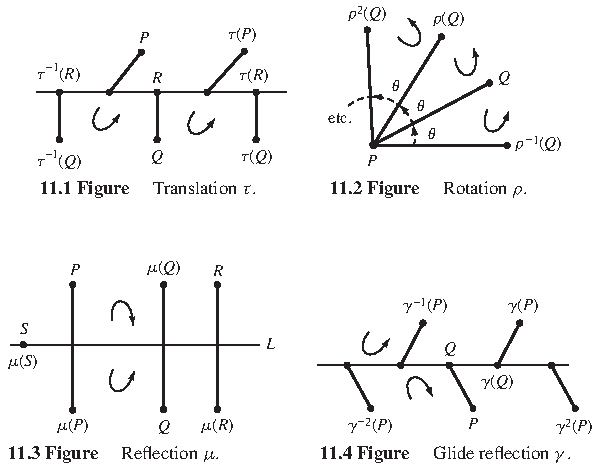
\includegraphics[width=0.819\linewidth,height=.8\textheight,keepaspectratio]{assets/p123_02.pdf}\end{center}
\end{BookFloat}

The theorem that follows describes the possible structures of finite subgroups of the full isometry group.

\BookLabel{11.5 Theorem} Every finite group \BookInline{G} of isometries of the plane is isomorphic to either the Klein 4-group, \BookInline{\mathbb{Z}_{n}} for \BookInline{n\geq 1,\allowbreak } or \BookInline{D_{n}} for some \BookInline{n\geq 3.}

\BookLabel{\textit{Proof}} \textbf{(Outline)} First we show that there is a point in the plane that is fixed by every element of \BookInline{G.} We let \BookInline{G= \{\phi _{1},\allowbreak \phi _{2},\allowbreak \phi _{3},\allowbreak...,\allowbreak \phi _{m}\}} and \BookInline{(x_{i},\allowbreak y_{i})= \phi _{i}(0,\allowbreak 0).} Then the point

\begin{center}\begin{adjustbox}{max width=\linewidth}\BookInline{\displaystyle P = (\overline{x},\allowbreak  \overline{y}) = \left( \frac{x_1 + x_2 + x_3 + \cdots + x_m}{m},\allowbreak  \frac{y_1 + y_1 + y_3 + \cdots + y_m}{m} \right)}\end{adjustbox}\end{center}

\noindent is the center of mass of the set \BookInline{S= \{(x_{i},\allowbreak y_{i})\mid 1\leq i\leq m\}} where each point is weighted by the number of \BookInline{\phi _{i}} that map (0, 0) to that point. It is easy to see that the isometries in \BookInline{G} permute the points in \BookInline{S} since for each \BookInline{i} and \BookInline{j,\allowbreak \phi _{i}\circ \phi _{j}= \phi _{k}} for some \BookInline{k.} Thus \BookInline{\phi _{i}(x_{j},\allowbreak y_{j})= } \BookInline{(x_{k},\allowbreak y_{k}).} This implies the center of mass of \BookInline{\phi (S)} is the same as the center of mass of \BookInline{S.} It can be shown that given the distances from the center of mass to the points of the set \BookInline{S,\allowbreak } the center of mass is the only point having these distances from the points of \BookInline{S.} This says that \BookInline{(x,\allowbreak y)} is fixed by every isometry in \BookInline{G.}

\end{BookBody}

% Source PDF page 124; original printed page 107
\BookSource{124}{107}
\BookNarrativetrue

\begin{BookBody}

The orientation preserving isometries of \BookInline{G} form a subgroup \BookInline{H} of \BookInline{G} which is either all of \BookInline{G} or else of order \BookInline{m/2.} You are asked to prove this in Exercise 22. Of course \BookInline{H} consists of the identity and possibly rotations about the point \BookInline{(x,\allowbreak y).} If \BookInline{H} has only one element, then \BookInline{G} has one or two elements and is therefore isomorphic with \BookInline{\mathbb{Z}_{1}} or \BookInline{\mathbb{Z}_{2}.} If \BookInline{H} has two elements, then \BookInline{G} has two or four elements and is therefore isomorphic with either the Klein 4-group\BookInline{,\allowbreak \mathbb{Z}_{4},\allowbreak } or \BookInline{\mathbb{Z}_{2}.} So we can assume that \BookInline{H} has at least three elements.

If we choose a rotation \BookInline{\rho } in \BookInline{H} that rotates through the smallest positive angle \BookInline{\theta } among all the elements of \BookInline{H,\allowbreak \rho } generates \BookInline{H.} The proof of this fact is similar to the proof that a subgroup of a cyclic group is cyclic and you are asked to provide the details of the proof in Exercise 23. If \BookInline{G= H,\allowbreak } then \BookInline{G} is isomorphic with \BookInline{\mathbb{Z}_{m}.} So we now assume that \BookInline{G} contains a reflection, say \BookInline{\mu.} Then the coset \BookInline{\mu H} contains only isometries of \BookInline{G} that reverse orientation. Each coset \BookInline{H} and \BookInline{\mu H} contains half the elements of \BookInline{G,\allowbreak } so \BookInline{G= H\cup \mu H.}

Consider now a regular \BookInline{n-}gon (recall that we are assuming that \BookInline{n\geq 3)} with center the point \BookInline{(x,\allowbreak y)} and having a vertex \BookInline{v_{0}} on the line fixed by \BookInline{\mu.} Each element of \BookInline{G} permutes the vertices of the \BookInline{n-}gon and preserves edges. Furthermore, no two elements of \BookInline{G} permute the vertices in the same way. Thus \BookInline{G} is isomorphic with a subgroup of the dihedral group \BookInline{D_{n}.} Since \BookInline{|G|= |D_{n}|,\allowbreak G} is isomorphic with \BookInline{D_{n}.}\BookEnd{\blacklozenge}

In Theorem 11.5 the Klein 4-group\BookInline{,\allowbreak V,\allowbreak } seems like an exception. However\BookInline{,\allowbreak V} fits into the family of dihedral groups since \BookInline{V} has two elements of order \BookInline{2,\allowbreak a} and \BookInline{b,\allowbreak } with the property that \BookInline{ab= ba^{- 1}.} Sometimes \BookInline{V} is denoted \BookInline{D_{2}} and considered a dihedral group. The isometries of the plane that map a line segment to itself are isomorphic with \BookInline{V.}

The preceding theorem gives the complete story about finite plane isometry groups. We turn now to some infinite groups of plane isometries that arise naturally in decorating and art. Among these are the\textit{ discrete frieze groups}. A discrete frieze consists of a pattern of finite width and height that is repeated endlessly in both directions along its baseline to form a strip of infinite length but finite height; think of it as a decorative border strip that goes around a room next to the ceiling on wallpaper. We consider those isometries that carry each basic pattern onto itself or onto another instance of the pattern in the frieze. The set of all such isometries is called the\textbf{ “frieze group.”} All discrete frieze groups are infinite and have a subgroup isomorphic to \BookInline{\mathbb{Z}} generated by the translation that slides the frieze lengthwise until the basic pattern is superimposed on the position of its next neighbor pattern in that direction. As a simple example of a discrete frieze, consider integral signs spaced equal distances apart and continuing infinitely to the left and right, indicated schematically like this.

\begin{BookFloat}{11_plane_isometries-p124-5}
\begin{center}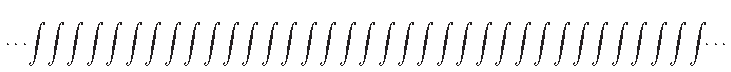
\includegraphics[width=1.000\linewidth,height=.8\textheight,keepaspectratio]{assets/p124_05.pdf}\end{center}
\end{BookFloat}

\noindent Let us consider the integral signs to be one unit apart. The symmetry group of this frieze is generated by a translation \BookInline{\tau } sliding the plane one unit to the right, and by a rotation \BookInline{\rho } of \BookInline{180^{\circ }} about a point in the center of some integral sign. There are no horizontal or vertical reflections, and no glide reflections. This frieze group is nonabelian; we can check that \BookInline{\tau \rho = \rho \tau ^{- 1}.} This relation between \BookInline{\tau } and \BookInline{\rho } looks very familiar. The dihedral group \BookInline{D_{n}} is also generated by two elements \BookInline{\rho } and \BookInline{\mu } that satisfy the relation \BookInline{\rho \mu = \mu \rho ^{- 1}.} If \BookInline{\tau } and \BookInline{\rho } in the frieze group are replaced by \BookInline{\rho } and \BookInline{\mu,\allowbreak } respectively, we have the same relation. In \BookInline{D_{n},\allowbreak \mu } has order 2, as does \BookInline{\rho } in the frieze group, but the element \BookInline{\rho } in \BookInline{D_{n}} has order \BookInline{n} while \BookInline{\tau } has infinite order. Thus it is natural to use the notation \BookInline{D_{\infty }} for this nonabelian frieze group.

As another example, consider the frieze given by an infinite string of D’s.

\BookTextHeading{\ensuremath{\cdot} \ensuremath{\cdot} \ensuremath{\cdot} \textbf{D D D D D D D D D D D}\ensuremath{\cdot} \ensuremath{\cdot} \ensuremath{\cdot}    }

\end{BookBody}

% Source PDF page 125; original printed page 108
\BookSource{125}{108}
\BookNarrativetrue

\begin{BookBody}

\noindent Its group is generated by a translation \BookInline{\tau } one step to the right and by a vertical reflection \BookInline{\mu } across a horizontal line cutting through the middle of all the D’s. We can check that these group generators commute this time, that is\BookInline{,\allowbreak \tau \mu = \mu \tau,\allowbreak } so this frieze group is abelian and is isomorphic to \BookInline{\mathbb{Z}\times \mathbb{Z}_{2}.}

It can be shown that if we classify such discrete friezes only by whether or not their groups contain a

\begin{center}\begin{adjustbox}{max width=\linewidth}\BookInline{\displaystyle \begin{aligned}&\;\text{rotation horizontal axis re}\;\text{fl}\;\text{ection}\; \\ &\;\text{vertical axis re}\;\text{fl}\;\text{ection nontrivial glide re}\;\text{fl}\;\text{ection}\;\end{aligned}}\end{adjustbox}\end{center}

\noindent then there are a total of seven possibilities. A\textit{ nontrivial glide reflection} in a symmetry group is one that is not equal to a product of a translation in that group and a reflection in that group. The group for the string of D’s above contains glide reflections across the horizontal line through the centers of the D’s, but the translation component of each glide reflection is also in the group so they are all considered trivial glide reflections in that group. The frieze group for

\begin{BookFloat}{11_plane_isometries-p125-4}
\begin{center}
\includegraphics[width=1.000\linewidth,height=.8\textheight,keepaspectratio]{assets/p125_04.pdf}\end{center}
\end{BookFloat}

\noindent contains a nontrivial glide reflection whose translation component is not an element of the group. The exercises exhibit the seven possible cases, and ask you to tell, for each case, which of the four types of isometries displayed above appear in the symmetry group. We do not obtain seven different group structures. Each of the groups obtained can be shown to be isomorphic to one of

\begin{center}\begin{adjustbox}{max width=\linewidth}\BookInline{\displaystyle \mathbb{Z},\allowbreak D_{\infty },\allowbreak \mathbb{Z}\times \mathbb{Z}_{2},\allowbreak \;\text{or}\;D_{\infty }\times \mathbb{Z}_{2}.}\end{adjustbox}\end{center}

Equally interesting is the study of symmetries when a pattern in the shape of a square, parallelogram, rhombus, or hexagon is repeated by translations along\textit{ two non}\textit{parallel vector directions} to fill the entire plane, like patterns that appear on wallpaper. These groups are called the\textit{ wallpaper groups} or the\textit{ plane crystallographic groups}. While a frieze could not be carried into itself by a rotation through a positive angle less than \BookInline{180^{\circ },\allowbreak } it is possible to have rotations of \BookInline{60^{\circ },\allowbreak 90^{\circ },\allowbreak 120^{\circ },\allowbreak } and \BookInline{180^{\circ }} for some of these plane-filling patterns. Figure 11.6 provides an illustration where the pattern consists of a square. We are interested in the group of plane isometries that carry this square onto itself or onto another square. Generators for this group are given by two translations (one sliding a square to the next neighbor to the right and one to the next above), by a rotation through \BookInline{90^{\circ }} about the center of a square, and by a reflection in a vertical (or horizontal) line along the edges of the square. The one reflection is all that is needed to “turn the plane over”; a diagonal reflection can also be used. After being turned over, the translations and rotations can be used again. The isometry group for this\textit{ periodic} \textit{pattern} in the plane surely contains a subgroup isomorphic to \BookInline{\mathbb{Z}\times \mathbb{Z}} generated by the unit translations to the right and upward, and a subgroup isomorphic to \BookInline{D_{4}} generated by those isometries that carry one square (it can be any square) into itself.

If we consider the plane to be filled with parallelograms as in Fig. 11.7, we do not get all the types of isometries that we did for Fig. 11.6. The symmetry group this time is generated by the translations indicated by the arrows and a rotation through \BookInline{180^{\circ }} about any vertex of a parallelogram.

It can be shown that there are 17 different types of wallpaper patterns when they are classified according to the types of rotations, reflections, and nontrivial glide reflections that they admit. We refer you to Gallian [8] for pictures of these 17 possibilities and a chart to help you identify them. The exercises illustrate a few of them. The situation

\end{BookBody}

% Source PDF page 126; original printed page 109
\BookSource{126}{109}
\BookNarrativetrue

\begin{BookBody}

\begin{BookFloat}{11_plane_isometries-p126-0}
\begin{center}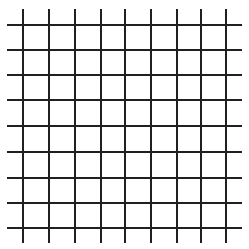
\includegraphics[width=0.341\linewidth,height=.8\textheight,keepaspectratio]{assets/p126_00.pdf}\end{center}
\begin{center}\small\textbf{11.6 Figure}\end{center}
\end{BookFloat}

\begin{BookFloat}{11_plane_isometries-p126-1}
\begin{center}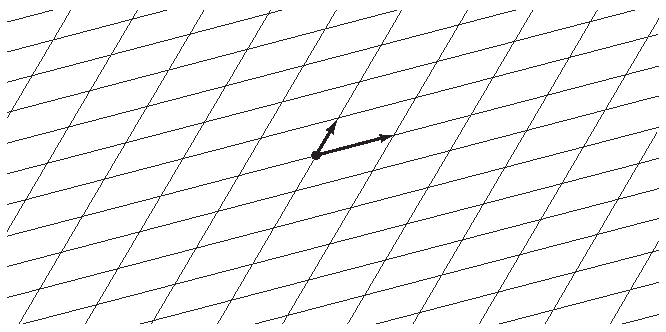
\includegraphics[width=0.913\linewidth,height=.8\textheight,keepaspectratio]{assets/p126_02.pdf}\end{center}
\begin{center}\small\textbf{11.7 Figure}\end{center}
\end{BookFloat}

\noindent in space is more complicated; it can be shown that there are 230 three-dimensional crystallographic groups. The final exercise we give involves rotations in space.

M. C. Escher (1898–1973) was an artist whose work included plane-filling patterns. In the exercises you are asked to analyze two of his works of this type.

\end{BookBody}

\BookNarrativefalse

\begin{BookBody}

\BookExerciseTitle{11}

\BookExercise{1.}{This exercise shows that the group of symmetries of a certain type of geometric figure may depend on the dimension of the space in which we consider the figure to lie.}

\BookExercise{a.}{Describe all symmetries of a point in the real line \BookInline{\mathbb{R};} that is, describe all isometries of \BookInline{\mathbb{R}} that leave one point fixed.}

\BookExercise{b.}{Describe all symmetries (translations, reflections, etc.) of a point in the plane \BookInline{\mathbb{R}^{2}.}}

\BookExercise{c.}{Describe all symmetries of a line segment in \BookInline{\mathbb{R}.}}

\BookExercise{d.}{Describe all symmetries of a line segment in \BookInline{\mathbb{R}^{2}.}}

\BookExercise{e.}{Describe some symmetries of a line segment in \BookInline{\mathbb{R}^{3}.}}

\BookExercise{2.}{Let \BookInline{P} stand for an orientation preserving plane isometry and \BookInline{R} for an orientation reversing one. Fill in the table with \BookInline{P} or \BookInline{R} to denote the orientation preserving or reversing property of a product.}

\end{BookBody}

% Source PDF page 127; original printed page 110
\BookSource{127}{110}
\BookNarrativefalse

\begin{BookBody}

\begin{BookFloat}{11_plane_isometries-p127-0}
\begin{center}\begin{adjustbox}{max width=\linewidth}
\renewcommand{\arraystretch}{1.2}\setlength{\tabcolsep}{5pt}
\begin{tabular}{c|c|c}
 & \BookInline{P} & \BookInline{R}\\\hline
\BookInline{P} &  & \\\hline
\BookInline{R} &  & \\
\end{tabular}
\end{adjustbox}\end{center}
\end{BookFloat}

\BookExercise{3.}{Fill in the table to give\textit{ all} possible types of plane isometries given by a product of two types as indicated in Tables 11.1 through 11.4. For example, a product of two rotations may be a rotation, or it may be another type. Fill in the box corresponding to \BookInline{\rho \rho } with both letters. Use your answer to Exercise 2 to eliminate some types. Eliminate the identity from consideration.}

\begin{BookFloat}{11_plane_isometries-p127-2}
\begin{center}\begin{adjustbox}{max width=\linewidth}
\renewcommand{\arraystretch}{1.2}\setlength{\tabcolsep}{5pt}
\begin{tabular}{c|c|c|c|c}
 & \BookInline{\tau } & \BookInline{\rho } & \BookInline{\mu } & \BookInline{\gamma }\\\hline
\BookInline{\tau } &  &  &  & \\\hline
\BookInline{\rho } &  &  &  & \\\hline
\BookInline{\mu } &  &  &  & \\\hline
\BookInline{\gamma } &  &  &  & \\
\end{tabular}
\end{adjustbox}\end{center}
\end{BookFloat}

\BookExercise{4.}{Draw a plane figure that has a one-element group as its group of symmetries in \BookInline{\mathbb{R}^{2}.}}

\BookExercise{5.}{Draw a plane figure that has a two-element group as its group of symmetries in \BookInline{\mathbb{R}^{2}.}}

\BookExercise{6.}{Draw a plane figure that has a three-element group as its group of symmetries in \BookInline{\mathbb{R}^{2}.}}

\BookExercise{7.}{Draw a plane figure that has a four-element group isomorphic to \BookInline{\mathbb{Z}_{4}} as its group of symmetries in \BookInline{\mathbb{R}^{2}.}}

\BookExercise{8.}{Draw a plane figure that has a four-element group isomorphic to the Klein 4-group \BookInline{V} as its group of symmetries in \BookInline{\mathbb{R}^{2}.}}

\BookExercise{9.}{For each of the four types of plane isometries (other than the identity), give the possibilities for the order of an isometry of that type in the group of plane isometries.}

\BookExercise{10.}{A plane isometry \BookInline{\phi } has a \BookInline{\text{fi}xed} \textit{point} if there exists a point \BookInline{P} in the plane such that \BookInline{\phi (P)= P.} Which of the four types of plane isometries (other than the identity) can have a fixed point?}

\BookExercise{11.}{Referring to Exercise 10, which types of plane isometries, if any, have exactly one fixed point?}

\BookExercise{12.}{Referring to Exercise 10, which types of plane isometries, if any, have exactly two fixed points?}

\BookExercise{13.}{Referring to Exercise 10, which types of plane isometries, if any, have an infinite number of fixed points?}

\BookExercise{14.}{Argue geometrically that a plane isometry that leaves three noncolinear points fixed must be the identity map.}

\BookExercise{15.}{Using Exercise 14, show algebraically that if two plane isometries \BookInline{\phi } and \BookInline{\psi } agree on three noncolinear points, that is, if \BookInline{\phi (P_{i})= \psi (P_{i})} for noncolinear points \BookInline{P_{1},\allowbreak P_{2},\allowbreak } and \BookInline{P_{3},\allowbreak } then \BookInline{\phi } and \BookInline{\psi } are the same map.}

\BookExercise{16.}{Do the rotations, together with the identity map, form a subgroup of the group of plane isometries? Why or why not?}

\BookExercise{17.}{Do the translations, together with the identity map, form a subgroup of the group of plane isometries? Why or why not?}

\BookExercise{18.}{Do the rotations about one particular point \BookInline{P,\allowbreak } together with the identity map, form a subgroup of the group of plane isometries? Why or why not?}

\BookExercise{19.}{Does the reflection across one particular line \BookInline{L,\allowbreak } together with the identity map, form a subgroup of the group of plane isometries? Why or why not?}

\BookExercise{20.}{Do the glide reflections, together with the identity map, form a subgroup of the group of plane isometries? Why or why not?}

\BookExercise{21.}{Which of the four types of plane isometries can be elements of a\textit{ finite} subgroup of the group of plane isometries?}

\BookExercise{22.}{Completing a detail of the proof of Theorem 11.5, let \BookInline{G} be a finite group of plane isometries. Show that the rotations in \BookInline{G,\allowbreak } together with the identity isometry, form a subgroup \BookInline{H} of \BookInline{G,\allowbreak } and that either \BookInline{H= G} or \BookInline{|G|= 2|H|.[}\textit{Hint:} Use the same method that we used to show that \BookInline{|S|= 2|A|.]}}

\end{BookBody}

% Source PDF page 128; original printed page 111
\BookSource{128}{111}
\BookNarrativefalse

\begin{BookBody}

\BookExercise{23.}{Completing a detail in the proof of Theorem 11.5, let \BookInline{G} be a finite group consisting of the identity isometry and rotations about one point \BookInline{P} in the plane. Show that \BookInline{G} is cyclic, generated by the rotation in \BookInline{G} that turns the plane counterclockwise about \BookInline{P} through the smallest angle \BookInline{\theta >0.[}\textit{Hint:} Follow the idea of the proof that a subgroup of a cyclic group is cyclic.]}

\noindent Exercises 24 through 30 illustrate the seven different types of friezes when they are classified according to their symmetries. Imagine the figure shown to be continued infinitely to the right and left. The symmetry group of a frieze always contains translations. For each of these exercises answer these questions about the symmetry group of the frieze.

\BookExercise{a.}{Does the group contain a rotation?}

\BookExercise{b.}{Does the group contain a reflection across a horizontal line?}

\BookExercise{c.}{Does the group contain a reflection across a vertical line?}

\BookExercise{d.}{Does the group contain a nontrivial glide reflection?}

\BookExercise{e.}{To which of the possible groups \BookInline{\mathbb{Z},\allowbreak D_{\infty },\allowbreak \mathbb{Z}\times \mathbb{Z}_{2},\allowbreak } or \BookInline{D_{\infty }\times \mathbb{Z}_{2}} do you think the symmetry group of the frieze is isomorphic?}

\BookExercise{24.}{\textbf{ F F F F F F F F F F F F F F F}}

\BookExercise{25.}{\textbf{ T T T T T T T T T T}}

\BookExercise{26.}{\textbf{ E E E E E E E E E E E E}}

\BookExercise{27.}{\textbf{ Z Z Z Z Z Z Z Z Z Z Z Z}}

\BookExercise{28.}{\textbf{ H H H H H H H H H H}}

\begin{BookFloat}{11_plane_isometries-p128-12}
\begin{center}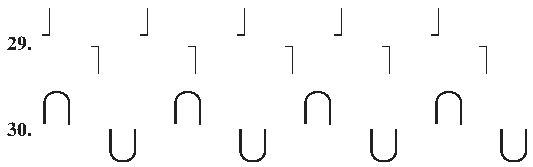
\includegraphics[width=0.731\linewidth,height=.8\textheight,keepaspectratio]{assets/p128_08.pdf}\end{center}
\end{BookFloat}

\noindent Exercises 31 through 37 describe a pattern to be used to fill the plane by translation in the two directions given by the specified vectors. Answer these questions in each case.

\BookExercise{a.}{Does the symmetry group contain any rotations? If so, through what possible angles \BookInline{\theta } where \BookInline{0<\theta \leq } \BookInline{180^{\circ }}?}

\BookExercise{b.}{Does the symmetry group contain any reflections?}

\BookExercise{c.}{Does the symmetry group contain any nontrivial glide reflections?}

\BookExercise{31.}{A square with horizontal and vertical edges using translation directions given by vectors (1, 0) and (0, 1).}

\BookExercise{32.}{A square as in Exercise 31 using translation directions given by vectors \BookInline{(1,\allowbreak 1/2)} and (0, 1).}

\BookExercise{33.}{A square as in Exercise 31 with the letter L at its center using translation directions given by vectors (1, 0) and (0, 1).}

\BookExercise{34.}{A square as in Exercise 31 with the letter E at its center using translation directions given by vectors (1, 0) and (0, 1).}

\BookExercise{35.}{A square as in Exercise 31 with the letter H at its center using translation directions given by vectors (1, 0) and (0, 1).}

\BookExercise{36.}{A regular hexagon with a vertex at the top using translation directions given by vectors (1, 0) and \BookInline{(1,\allowbreak \sqrt{3}).}}

\BookExercise{37.}{A regular hexagon with a vertex at the top containing an equilateral triangle with vertex at the top and centroid at the center of the hexagon, using translation directions given by vectors (1, 0) and \BookInline{(1,\allowbreak \sqrt{3}).}}

\noindent Exercises 38 and 39 are concerned with art works of M. C. Escher. Find images of the indicated art by searching on the internet. Neglect the shading and colors in the figures and assume the markings in each human figure, reptile, 
% Source PDF page 129; original printed page 112
\BookSource{129}{112}
or horseman are the same, even though they may be invisible due to shading. Answer the same questions (a), (b), and (c) that were asked for Exercises 31 through 36, and also answer this part (d).

\end{BookBody}

\BookNarrativefalse

\begin{BookBody}

\BookExercise{d.}{Assuming horizontal and vertical coordinate axes with equal scales as usual, give vectors in the two nonparallel directions of vectors that generate the translation subgroup. Do not concern yourself with the length of these vectors.}

\BookExercise{38.}{\textit{ The Study of Regular Division of the Plane with Horsemen}.}

\BookExercise{39.}{\textit{ The Study of Regular Division of the Plane with Reptiles}.}

\BookExercise{40.}{Let \BookInline{\phi:\mathbb{R}\to U} be given by \BookInline{\phi (\theta )= } cos\BookInline{(\theta )+ i} sin\BookInline{(\theta )} and \BookInline{S= \phi [\mathbb{Z}].}}

\BookExercise{a.}{Show that any rotation mapping \BookInline{S} to \BookInline{S} is a rotation by an angle \BookInline{n\in \mathbb{Z}} where angles are measured in radians. \textbf{b.} Show that reflection across the \BookInline{x-}axis maps \BookInline{S} to \BookInline{S.}}

\BookExercise{c.}{What is the group of symmetries of \BookInline{S}?}

\BookExercise{41.}{Show that the rotations of a cube in space form a group isomorphic to \BookInline{S_{4}.[}\textit{Hint:} A rotation of the cube permutes the diagonals through the center of the cube.]}

\end{BookBody}
\ifdefined\BookMaster\let\BookFinish\relax\else\def\BookFinish{\end{document}}\fi\BookFinish

\clearpage
% !TeX program = xelatex
\ifdefined\BookMaster\else
\documentclass[11pt,oneside]{article}
% !TeX program = xelatex
\usepackage[b5paper,left=22mm,right=22mm,top=20mm,bottom=22mm,footskip=11mm]{geometry}
\usepackage{fontspec}
\setmainfont{TeX Gyre Termes}
\setsansfont{TeX Gyre Heros}
\usepackage{amsmath,amssymb,mathtools,amsthm}
\renewcommand{\cdots}{\mathinner{\cdotp\cdotp\cdotp}}
\usepackage{graphicx,adjustbox,array,booktabs,longtable,multirow,enumitem,changepage,needspace}
\usepackage[table]{xcolor}
\usepackage{fancyhdr}
\raggedbottom
\interfootnotelinepenalty=10000
\newcommand{\BookFootnote}[2]{\begingroup\renewcommand{\thefootnote}{\fnsymbol{footnote}}\footnote[#1]{#2}\endgroup}
\newcommand{\BookFootnoteMark}[1]{\begingroup\renewcommand{\thefootnote}{\fnsymbol{footnote}}\footnotemark[#1]\endgroup}
\newcommand{\BookFootnoteText}[2]{\begingroup\renewcommand{\thefootnote}{\fnsymbol{footnote}}\footnotetext[#1]{#2}\endgroup}
\newenvironment{BookFloat}[1]{\par\addvspace{.6\baselineskip}\noindent\def\BookFloatID{#1}\begin{minipage}{\linewidth}\phantomsection\label{bookfloat:#1:start}}{\phantomsection\label{bookfloat:\BookFloatID:end}\end{minipage}\par\addvspace{.6\baselineskip}}

\usepackage[unicode,hidelinks]{hyperref}
\pagestyle{fancy}
\fancyhf{}
\newcommand{\BookFooter}{}
\fancyfoot[L]{\parbox[b]{\dimexpr\textwidth-15mm}{\footnotesize\BookFooter}}
\fancyfoot[R]{\footnotesize\thepage}
\renewcommand{\headrulewidth}{0pt}
\renewcommand{\footrulewidth}{0pt}
\setlength{\parindent}{0pt}
\setlength{\parskip}{0.2em}
\setlength{\emergencystretch}{3em}
\setlist{nosep,leftmargin=1.7em,labelsep=.65em}
\newif\ifBookNarrative
\BookNarrativetrue
\newenvironment{BookBody}{\setlength{\parindent}{0pt}}{}
\newcommand{\BookStatement}[1]{\par\addvspace{.6\baselineskip}\noindent #1\enspace\ignorespaces}
\newcommand{\BookLabel}[1]{\par\addvspace{.6\baselineskip}\needspace{3\baselineskip}\noindent\textbf{#1}\quad\ignorespaces}
\newcommand{\BookHeading}[1]{\par\addvspace{\baselineskip}\needspace{4\baselineskip}\noindent{\large\bfseries #1}\par\medskip}
\newcommand{\BookSubheading}[1]{\par\addvspace{.7\baselineskip}\needspace{3\baselineskip}\noindent{\bfseries #1}\par\smallskip}
\newcommand{\BookTextHeading}[1]{\par\addvspace{.7\baselineskip}\needspace{3\baselineskip}\noindent #1\par\smallskip}
\newcommand{\BookSectionTitle}[2]{\par\addvspace{1.2\baselineskip}\needspace{5\baselineskip}\noindent\colorbox{gray!25}{\sffamily\bfseries\small SECTION #1}\quad{\large\bfseries #2}\par\medskip}
\newcommand{\BookExerciseTitle}[1]{\par\addvspace{\baselineskip}\needspace{4\baselineskip}\noindent{\color{gray}\rule{1.5mm}{1.5mm}}\enspace{\large\bfseries Exercises #1}\par\medskip}
\newcommand{\BookBullet}[1]{\begin{list}{\textbullet}{\setlength{\leftmargin}{1.7em}\setlength{\labelwidth}{1em}\setlength{\labelsep}{.7em}\setlength{\topsep}{0pt}\setlength{\parsep}{0pt}\setlength{\itemsep}{0pt}}\item #1\end{list}}
\newcommand{\BookExercise}[2]{\begin{list}{\textbf{#1}}{\setlength{\leftmargin}{2.2em}\setlength{\labelwidth}{1.5em}\setlength{\labelsep}{.7em}\setlength{\topsep}{.15em}\setlength{\parsep}{0pt}\setlength{\itemsep}{0pt}}\item #2\end{list}}
\newcommand{\BookEnd}[1]{\unskip\nobreak\hfill\ensuremath{#1}}
\newcommand{\BookSource}[2]{\phantomsection\label{sourcepage:#1}} % Source-page anchors, retained through reflow.
\usepackage{multicol}
\usepackage{tikz}
\newcommand{\BookPartEntry}[2]{\par\noindent\makebox[17mm][l]{\bfseries Section #1}#2\par}
\newcommand{\BookPartTitle}[3]{\par\bigskip\noindent\begin{tikzpicture}\node[anchor=north west,inner sep=0pt,outer sep=0pt] (bookpart) at (0,0) {\begin{minipage}{\dimexpr\linewidth-.5pt}\hspace*{26mm}\begin{minipage}[t]{\dimexpr\linewidth-26mm}\begin{adjustbox}{max width=\linewidth}{\fontsize{20}{24}\selectfont\bfseries #2}\end{adjustbox}\par\vspace{6mm}\hrule\vspace{6mm}{\sffamily\footnotesize\setlength{\parskip}{.3em}#3}\vspace{3mm}\end{minipage}\end{minipage}};\path[shade,top color=gray!60,bottom color=white] (0,0) rectangle ([xshift=24mm]bookpart.south west);\node[anchor=north,font=\sffamily\bfseries\small] at (12mm,-2mm) {PART};\node[anchor=north,font=\sffamily\bfseries\Huge] at (12mm,-7mm) {#1};\end{tikzpicture}\par\bigskip}
\newsavebox{\BookMathBox}
\makeatletter
\newcommand{\BookInline}[1]{\leavevmode\hskip0pt\relax\begingroup\in@{\begin}{#1}\ifin@\sbox{\BookMathBox}{\(#1\)}\ifdim\wd\BookMathBox>\dimexpr\linewidth-1em\relax\resizebox{\dimexpr\linewidth-1em\relax}{!}{\usebox{\BookMathBox}}\else\(#1\)\fi\else\in@{\left}{#1}\ifin@\sbox{\BookMathBox}{\(#1\)}\ifdim\wd\BookMathBox>\dimexpr\linewidth-1em\relax\resizebox{\dimexpr\linewidth-1em\relax}{!}{\usebox{\BookMathBox}}\else\(#1\)\fi\else\(#1\)\fi\fi\endgroup\hskip0pt\relax}
\makeatother
\DeclareMathOperator{\Aut}{Aut}
\DeclareMathOperator{\End}{End}
\DeclareMathOperator{\Hom}{Hom}
\DeclareMathOperator{\GF}{GF}
\DeclareMathOperator{\irr}{irr}
\DeclareMathOperator{\lt}{lt}
\DeclareMathOperator{\lp}{lp}
\providecommand{\textcircled}[1]{\textnormal{(#1)}}

\begin{document}
\fi
\renewcommand{\BookFooter}{Section 12 Factor Groups}
\pdfbookmark[0]{Section 12 Factor Groups}{12_factor_groups}
\ifdefined\BookMaster\else\setcounter{page}{113}\fi
% Source PDF page 130; original printed page 113
\BookSource{130}{113}
\BookPartTitle{III}{Homomorphisms and Factor Groups}{\BookPartEntry{12}{Factor Groups}
\BookPartEntry{13}{Factor-Group Computations and Simple Groups}
\BookPartEntry{14}{Group Action on a Set}
\BookPartEntry{15}{Applications of G-Sets to Counting}}

\BookNarrativetrue

\begin{BookBody}

\BookSectionTitle{12}{Factor Groups}

\noindent Recall from Section 10 that for some group tables we can arrange the head on top and on the left so that the elements are grouped into left cosets of a subgroup in such a way that the coset blocks form a group table. We start this section by looking more closely at why the cosets of \BookInline{\{0,\allowbreak 3\}\leq \mathbb{Z}_{6}} form a group and why the cosets of the subgroup \BookInline{\{\iota,\allowbreak \mu \}\leq D_{3}} do not. Table 12.1 is the group table for \BookInline{\mathbb{Z}_{6}} with the heads at the top and left sorted by cosets of \BookInline{\{0,\allowbreak 3\}.}

\begin{BookFloat}{12_factor_groups-p130-8}
\begin{center}\small\textbf{12.1 Table}\end{center}
\begin{center}\begin{adjustbox}{max width=\linewidth}
\renewcommand{\arraystretch}{1.2}\setlength{\tabcolsep}{5pt}
\begin{tabular}{c|c|c|c|c|c|c}
\BookInline{+ _{6}} & 0 & 3 & \cellcolor[gray]{0.866}1 & \cellcolor[gray]{0.866}4 & \cellcolor[gray]{0.625}2 & \cellcolor[gray]{0.625}5\\\hline
0 & 0 & 3 & \cellcolor[gray]{0.866}1 & \cellcolor[gray]{0.866}4 & \cellcolor[gray]{0.625}2 & \cellcolor[gray]{0.625}5\\\hline
3 & 3 & 0 & \cellcolor[gray]{0.866}4 & \cellcolor[gray]{0.866}1 & \cellcolor[gray]{0.625}5 & \cellcolor[gray]{0.625}2\\\hline
\cellcolor[gray]{0.866}1 & \cellcolor[gray]{0.866}1 & \cellcolor[gray]{0.866}4 & \cellcolor[gray]{0.625}2 & \cellcolor[gray]{0.625}5 & 3 & 0\\\hline
\cellcolor[gray]{0.866}4 & \cellcolor[gray]{0.866}4 & \cellcolor[gray]{0.866}1 & \cellcolor[gray]{0.625}5 & \cellcolor[gray]{0.625}2 & 0 & 3\\\hline
\cellcolor[gray]{0.625}2 & \cellcolor[gray]{0.625}2 & \cellcolor[gray]{0.625}5 & 3 & 0 & \cellcolor[gray]{0.866}4 & \cellcolor[gray]{0.866}1\\\hline
\cellcolor[gray]{0.625}5 & \cellcolor[gray]{0.625}5 & \cellcolor[gray]{0.625}2 & 0 & 3 & \cellcolor[gray]{0.866}1 & \cellcolor[gray]{0.866}4\\
\end{tabular}
\end{adjustbox}\end{center}
\end{BookFloat}

\noindent According to Table 12.1 the coset \BookInline{\{1,\allowbreak 4\}} plus the coset \BookInline{\{2,\allowbreak 5\}} is the coset \BookInline{\{0,\allowbreak 3\}.} This means that if we add either 1 or 4 to either 2 or 5 in \BookInline{\mathbb{Z}_{6},\allowbreak } we should get either 0 or 3. This is easily checked by adding the four possibilities.

\begin{center}\begin{adjustbox}{max width=\linewidth}\BookInline{\displaystyle \begin{aligned}1+ _{6}2&= 3 \\ 1+ _{6}5&= 0 \\ 4+ _{6}2&= 0 \\ 4+ _{6}5&= 3\end{aligned}}\end{adjustbox}\end{center}

\noindent We observe that if we wish to break up a group into its left cosets so the group table shows an operation on the left cosets, we need to be sure that if \BookInline{a_{1},\allowbreak a_{2}} are in the same 
% Source PDF page 131; original printed page 114
\BookSource{131}{114}
left coset and \BookInline{b_{1},\allowbreak b_{2}} are in the same left coset, then \BookInline{a_{1}b_{1}} and \BookInline{a_{2}b_{2}} are in the same left coset. If this condition is satisfied for a subgroup \BookInline{H\leq G,\allowbreak } we say that the operation on the left cosets of \BookInline{H} is\textbf{ induced} by the operation of \BookInline{G} or that the operation of \BookInline{G} \textbf{induces} an operation on the left cosets of \BookInline{H.} In this case for any \BookInline{a,\allowbreak b\in G} we write

\end{BookBody}

\BookNarrativetrue

\begin{BookBody}

\begin{center}\begin{adjustbox}{max width=\linewidth}\BookInline{\displaystyle (aH)(bH)= (ab)H}\end{adjustbox}\end{center}

\noindent to mean that the product of any element in \BookInline{aH} multiplied by any element in \BookInline{bH} must be in the left coset \BookInline{(ab)H.}

\BookLabel{12.2 Example} We show that the operation \BookInline{+ } in the group \BookInline{\mathbb{Z}} induces an operation on the cosets of \BookInline{5\mathbb{Z}\leq \mathbb{Z}.} We first list the left cosets.

\begin{center}\begin{adjustbox}{max width=\linewidth}\BookInline{\displaystyle \begin{aligned}5\mathbb{Z}&= \{\cdots - 10,\allowbreak - 5,\allowbreak 0,\allowbreak 5,\allowbreak 10,\allowbreak ...\} \\ 1+ 5\mathbb{Z}&= \{\cdots - 9,\allowbreak - 4,\allowbreak 1,\allowbreak 6,\allowbreak 11,\allowbreak ...\} \\ 2+ 5\mathbb{Z}&= \{\cdots - 8,\allowbreak - 3,\allowbreak 2,\allowbreak 7,\allowbreak 12,\allowbreak ...\} \\ 3+ 5\mathbb{Z}&= \{\cdots - 7,\allowbreak - 2,\allowbreak 3,\allowbreak 8,\allowbreak 13,\allowbreak ...\} \\ 4+ 5\mathbb{Z}&= \{\cdots - 6,\allowbreak - 1,\allowbreak 4,\allowbreak 9,\allowbreak 14,\allowbreak ...\}\end{aligned}}\end{adjustbox}\end{center}

\noindent Let \BookInline{a_{1}} and \BookInline{a_{2}} be in the same left coset of \BookInline{5\mathbb{Z}.} Then \BookInline{a_{2}= a_{1}+ 5r} for some \BookInline{r\in \mathbb{Z}.} We also let \BookInline{b_{1},\allowbreak b_{2}} be in the same left coset of \BookInline{5\mathbb{Z}.} Then \BookInline{b_{2}= b_{1}+ 5s} for some \BookInline{s\in \mathbb{Z}.} We compute \BookInline{a_{2}+ b_{2}.}

\begin{center}\begin{adjustbox}{max width=\linewidth}\BookInline{\displaystyle \begin{aligned}a_{2}+ b_{2}&= (a_{1}+ 5r)+ (b_{1}+ 5s) \\ &= a_{1}+ 5r+ b_{1}+ 5s \\ &= a_{1}+ b_{1}+ 5r+ 5s(1) \\ &= (a_{1}+ b_{1})+ 5(r+ s)(2) \\ &\in (a_{1}+ b_{1})+ 5\mathbb{Z}\end{aligned}}\end{adjustbox}\end{center}

\noindent So \BookInline{a_{2}+ b_{2}} is in the same coset as \BookInline{a_{1}+ b_{1},\allowbreak } which says that addition in \BookInline{\mathbb{Z}} induces an operation on the five left cosets \BookInline{5\mathbb{Z},\allowbreak 1+ 5\mathbb{Z},\allowbreak 2+ 5\mathbb{Z},\allowbreak 3+ 5\mathbb{Z},\allowbreak 4+ 5\mathbb{Z}.} Looking back at the calculations, we see that only properties shared by all groups were used in each step except in line (1) where we used the fact that \BookInline{\mathbb{Z}} is abelian. Furthermore, line (2) is not necessary since \BookInline{5\mathbb{Z}} is a subgroup of \BookInline{\mathbb{Z}} so we know that \BookInline{5\mathbb{Z}} is closed under addition. From this example, it appears that as long as \BookInline{G} is an abelian group, the operation of \BookInline{G} induces an operation on the left cosets of any subgroup of \BookInline{G.}\BookEnd{\blacktriangle}

\noindent In Equation (1) of Example 12.2 we used the fact that \BookInline{5r+ b_{1}= b_{1}+ 5r.} If we were doing the same computation in multiplicative notation and using any group \BookInline{G} and subgroup \BookInline{H} of \BookInline{G,\allowbreak } this would correspond to \BookInline{hb_{1}= b_{1}h.} If the group \BookInline{G} is not abelian, then this computation fails. However, we can weaken the abelian condition slightly and still get an induced operation on the left cosets. All we really need is that \BookInline{hb_{1}= b_{1}h^{\prime }} for some \BookInline{h^{\prime }\in H.} This happens when the left coset \BookInline{b_{1}H} is the same set as the right coset \BookInline{Hb_{1}.}

\BookLabel{12.3 Definition} Let \BookInline{H} be a subgroup of \BookInline{G.} We say that \BookInline{H} is a\textbf{ normal} subgroup of \BookInline{G} if for all \BookInline{g\in G,\allowbreak } \BookInline{gH= Hg.} If \BookInline{H} is a normal subgroup of \BookInline{G,\allowbreak } we write \BookInline{H\unlhd G.}\BookEnd{\blacksquare}

Recall that Theorem 10.17 states that if \BookInline{\phi:G\to G^{\prime }} is a group homomorphism and \BookInline{e^{\prime }} is the identity element in \BookInline{G^{\prime },\allowbreak } then Ker\BookInline{(\phi )= \{g\in G\mid \phi (g)= e^{\prime }\}} has the property that left and right cosets of Ker\BookInline{(\phi )} are the same. So the kernel of any homomorphism is a normal subgroup.

\BookLabel{12.4 Example} The subgroup of even permutations \BookInline{A_{n}\leq S_{n}} is normal since \BookInline{A_{n}} is the kernel of the homomorphism sgn \BookInline{:S_{n}\to \{1,\allowbreak - 1\}.}\BookEnd{\blacktriangle}

\end{BookBody}

% Source PDF page 132; original printed page 115
\BookSource{132}{115}
\BookNarrativetrue

\begin{BookBody}

\BookLabel{12.5 Example} If \BookInline{H\leq G} and \BookInline{G} is an abelian group, then \BookInline{H} is a normal subgroup of \BookInline{G.} \BookEnd{\blacktriangle}

\BookLabel{12.6 Example} Let \BookInline{H= \{A\in } GL\BookInline{(n,\allowbreak \mathbb{R})\mid } det\BookInline{(A)= 1\}.} The determinant map satisfies det\BookInline{(AB)= } det\BookInline{(A)} det\BookInline{(B),\allowbreak } which means that the determinant map is a homomorphism, det: GL\BookInline{(n,\allowbreak \mathbb{R})\to \mathbb{R}^{\ast }.} Thus \BookInline{H= }Ker(det), which says that \BookInline{H\unlhd } GL\BookInline{(n,\allowbreak \mathbb{R}).} This subgroup \BookInline{H} is called the\textbf{ special linear group} and it is denoted by SL\BookInline{(n,\allowbreak \mathbb{R}).}\BookEnd{\blacktriangle}

\BookLabel{12.7 Theorem} Let \BookInline{H} be a subgroup of a group \BookInline{G.} Then left coset multiplication is well defined by the equation

\begin{center}\begin{adjustbox}{max width=\linewidth}\BookInline{\displaystyle (aH)(bH)= (ab)H}\end{adjustbox}\end{center}

\noindent if and only if \BookInline{H} is a normal subgroup of \BookInline{G.}

\BookLabel{\textit{Proof}} Suppose first that \BookInline{(aH)(bH)= (ab)H} does give a well-defined binary operation on left cosets. Let \BookInline{a\in G.} We want to show that \BookInline{aH} and \BookInline{Ha} are the same set. We use the standard technique of showing that each is a subset of the other.

Let \BookInline{x\in aH.} Choosing representatives \BookInline{x\in aH} and \BookInline{a^{- 1}\in a^{- 1}H,\allowbreak } we have \BookInline{(xH)(a^{- 1}H)= (xa^{- 1})H.} On the other hand, choosing representatives \BookInline{a\in aH} and \BookInline{a^{- 1}\in a^{- 1}H,\allowbreak } we see that \BookInline{(aH)(a^{- 1}H)= eH= H.} Using our assumption that left coset multiplication by representatives is well defined, we must have \BookInline{xa^{- 1}= h\in H.} Then \BookInline{x= ha,\allowbreak } so \BookInline{x\in Ha} and \BookInline{aH\subseteq Ha.} We leave the symmetric proof that \BookInline{Ha\subseteq aH} to Exercise 26.

We turn now to the converse: If \BookInline{H} is a normal subgroup, then left coset multiplication by representatives is well-defined. Due to our hypothesis, we can simply say\textit{ cosets,} omitting\textit{ left} and\textit{ right}. Suppose we wish to compute \BookInline{(aH)(bH).} Choosing \BookInline{a\in aH} and \BookInline{b\in bH,\allowbreak } we obtain the coset \BookInline{(ab)H.} Choosing different representatives \BookInline{ah_{1}\in aH} and \BookInline{bh_{2}\in bH,\allowbreak } we obtain the coset \BookInline{ah_{1}bh_{2}H.} We must show that these are the same cosets. Now \BookInline{h_{1}b\in Hb= bH,\allowbreak } so \BookInline{h_{1}b= bh_{3}} for some \BookInline{h_{3}\in H.} Thus

\begin{center}\begin{adjustbox}{max width=\linewidth}\BookInline{\displaystyle (ah_{1})(bh_{2})= a(h_{1}b)h_{2}= a(bh_{3})h_{2}= (ab)(h_{3}h_{2})}\end{adjustbox}\end{center}

\noindent and \BookInline{(ab)(h_{3}h_{2})\in (ab)H.} Therefore\BookInline{,\allowbreak ah_{1}bh_{2}} is in \BookInline{(ab)H.} \BookEnd{\blacklozenge}

Theorem 12.7 shows that we have an operation on the left cosets of \BookInline{H\leq G} induced by the operation on \BookInline{G} if and only if \BookInline{H} is a normal subgroup of \BookInline{G.} We next verify that this operation makes \BookInline{G/H,\allowbreak } the cosets of \BookInline{H} in \BookInline{G,\allowbreak } a group.

\BookLabel{12.8 Corollary} Let \BookInline{H} be a normal subgroup of \BookInline{G.} Then the cosets of \BookInline{H} form a group \BookInline{G/H} under the binary operation \BookInline{(aH)(bH)= (ab)H.}\BookEnd{\blacktriangle}

\BookLabel{\textit{Proof}} Computing\BookInline{,\allowbreak (aH)[(bH)(cH)]= (aH)[(bc)H]= [a(bc)]H,\allowbreak } and similarly, we have \BookInline{[(aH)(bH)](cH)= [(ab)c]H,\allowbreak } so associativity in \BookInline{G/H} follows from associativity in \BookInline{G.} Because \BookInline{(aH)(eH)= (ae)H= aH= (ea)H= (eH)(aH),\allowbreak } we see that \BookInline{eH= H} is the identity element in \BookInline{G/H.} Finally\BookInline{,\allowbreak (a^{- 1}H)(aH)= (a^{- 1}a)H= eH= (aa^{- 1})H= } \BookInline{(aH)(a^{- 1}H)} shows that \BookInline{a^{- 1}H= (aH)^{- 1}.}\BookEnd{\blacklozenge}

\BookLabel{12.9 Definition} The group \BookInline{G/H} in the preceding corollary is the\textbf{ factor group} (or\textbf{ quotient group}) of \BookInline{G} by \BookInline{H.}\BookEnd{\blacksquare}

\BookLabel{12.10 Example} Since \BookInline{\mathbb{Z}} is an abelian group\BookInline{,\allowbreak n\mathbb{Z}} is a normal subgroup. Corollary 12.8 allows us to construct the factor group \BookInline{\mathbb{Z}/n\mathbb{Z}.} For any integer \BookInline{m,\allowbreak } the division algorithm says that \BookInline{m= nq+ r} for some \BookInline{0\leq r<n.} Therefore\BookInline{,\allowbreak m\in r+ n\mathbb{Z}.} So \BookInline{\mathbb{Z}/n\mathbb{Z}= \{k+ n\mathbb{Z}\mid 0\leq k<} \BookInline{n\}.} Thus \BookInline{\langle 1+ n\mathbb{Z}\rangle = \mathbb{Z}/n\mathbb{Z},\allowbreak } which implies that \BookInline{\mathbb{Z}/n\mathbb{Z}} is cyclic and isomorphic with \BookInline{\mathbb{Z}_{n}.} \BookEnd{\blacktriangle}

\end{BookBody}

% Source PDF page 133; original printed page 116
\BookSource{133}{116}
\BookNarrativetrue

\begin{BookBody}

\BookLabel{12.11 Example} Consider the abelian group \BookInline{\mathbb{R}} under addition, and let \BookInline{c\in \mathbb{R}^{+ }.} The cyclic subgroup \BookInline{\langle c\rangle } of \BookInline{\mathbb{R}} contains as elements

\begin{center}\begin{adjustbox}{max width=\linewidth}\BookInline{\displaystyle \cdots - 3c,\allowbreak - 2c,\allowbreak - c,\allowbreak 0,\allowbreak c,\allowbreak 2c,\allowbreak 3c,\allowbreak \cdots .}\end{adjustbox}\end{center}

\noindent Every coset of \BookInline{\langle c\rangle } contains just one element \BookInline{x} such that \BookInline{0\leq x<c.} If we choose these elements as representatives of the cosets when computing in \BookInline{\mathbb{R}/\langle c\rangle,\allowbreak } we find that we are computing their sum modulo \BookInline{c} as discussed for the computation in \BookInline{\mathbb{R}_{c}} in Section 3. For example, if \BookInline{c= 5.37,\allowbreak } then the sum of the cosets \BookInline{4.65+ \langle 5.37\rangle } and \BookInline{3.42+ \langle 5.37\rangle } is the coset \BookInline{8.07+ \langle 5.37\rangle,\allowbreak } which contains \BookInline{8.07- 5.37= 2.7,\allowbreak } which is \BookInline{4.65+ _{5.37}3.42.} Working with these coset elements \BookInline{x} where \BookInline{0\leq x<c,\allowbreak } we thus see that the group \BookInline{\mathbb{R}_{c}} of Section 3 is isomorphic to \BookInline{\mathbb{R}/\langle c\rangle } under an isomorphism \BookInline{\psi } where \BookInline{\psi (x)= x+ \langle c\rangle } for all \BookInline{x\in \mathbb{R}_{c}.} Of course\BookInline{,\allowbreak \mathbb{R}/\langle c\rangle } is then also isomorphic to the circle group \BookInline{U} of complex numbers of magnitude 1 under multiplication\BookInline{.}\BookEnd{\blacktriangle}

We have seen that the group \BookInline{\mathbb{Z}/\langle n\rangle } is isomorphic to the group \BookInline{\mathbb{Z}_{n},\allowbreak } and as a set, \BookInline{\mathbb{Z}_{n}= \{0,\allowbreak 1,\allowbreak 3,\allowbreak 4,\allowbreak \cdots,\allowbreak n- 1\},\allowbreak } the set of nonnegative integers less than \BookInline{n.} Example 12.11 shows that the group \BookInline{\mathbb{R}/\langle c\rangle } is isomorphic to the group \BookInline{\mathbb{R}_{c}.} In Section 3, we choose the notation \BookInline{\mathbb{R}_{c}} rather than the conventional \BookInline{[0,\allowbreak c)} for the half-open interval of nonnegative real numbers less than \BookInline{c.} We did that to bring out now the comparison of these factor groups of \BookInline{\mathbb{Z}} with these factor groups of \BookInline{\mathbb{R}.}

\BookTextHeading{\textbf{Homomorphisms and Factor Groups}  }

\noindent We learned that the kernel of any homomorphism \BookInline{\phi:G\to G^{\prime }} is a normal subgroup of \BookInline{G.} Do all normal subgroups arise in this way? That is, for any normal subgroup \BookInline{H\unlhd G,\allowbreak } is there a group homomorphism \BookInline{\phi:G\to G^{\prime }} for some group \BookInline{G^{\prime }} such that \BookInline{H} is the kernel of \BookInline{G}? The answer to the question is yes as we see in Theorem 12.12.

\BookLabel{12.12 Theorem} Let \BookInline{H} be a normal subgroup of \BookInline{G.} Then \BookInline{\gamma:G\to G/H} given by \BookInline{\gamma (x)= xH} is a homomorphism with kernel \BookInline{H.}

\BookLabel{\textit{Proof}} Let \BookInline{x,\allowbreak y\in G.} Then

\begin{center}\begin{adjustbox}{max width=\linewidth}\BookInline{\displaystyle \gamma (xy)= (xy)H= (xH)(yH)= \gamma (x)\gamma (y),\allowbreak }\end{adjustbox}\end{center}

\noindent so \BookInline{\gamma } is a homomorphism. Since \BookInline{xH= H} if and only if \BookInline{x\in H,\allowbreak } we see that the kernel of \BookInline{\gamma } is indeed \BookInline{H.}\BookEnd{\blacklozenge}

Since the kernel of any homomorphism \BookInline{\phi:G\to G^{\prime }} is a normal subgroup, it is natural to ask how the factor group \BookInline{G/}Ker\BookInline{(\phi )} is related to \BookInline{G^{\prime }.} Theorem 12.12 and the next example illustrate that there is a very strong connection.

\BookLabel{12.13 Example} \textbf{(Reduction Modulo} \BookInline{n)} Let \BookInline{\phi:\mathbb{Z}\to \mathbb{Z}_{n}} be defined by letting \BookInline{\phi (m)} be the remainder when \BookInline{m} is divided by \BookInline{n.} We check that \BookInline{\phi } is a group homomorphism. Let \BookInline{m_{1},\allowbreak m_{2}\in \mathbb{Z}} and suppose that the division algorithm gives us

\begin{center}\begin{adjustbox}{max width=\linewidth}\BookInline{\displaystyle \begin{aligned}m_{1}&= nq_{1}+ r_{1}\;\text{and}\; \\ m_{2}&= nq_{2}+ r_{2}.\end{aligned}}\end{adjustbox}\end{center}

\noindent Then \BookInline{m_{1}+ m_{2}= n(q_{1}+ q_{2})+ r_{1}+ r_{2}.} If \BookInline{r_{1}+ r_{2}<n,\allowbreak } then

\begin{center}\begin{adjustbox}{max width=\linewidth}\BookInline{\displaystyle \phi (m_{1}+ m_{2})= r_{1}+ r_{2}= \phi (m_{1})+ _{n}\phi (m_{2}).}\end{adjustbox}\end{center}

\noindent On the other hand, if \BookInline{r_{1}+ r_{2}\geq n,\allowbreak } then \BookInline{m_{1}+ m_{2}= n(q_{1}+ q_{2}+ 1)+ (r_{1}+ r_{2}- n)} and \BookInline{0\leq r_{1}+ r_{2}- n<n,\allowbreak } which implies

\begin{center}\begin{adjustbox}{max width=\linewidth}\BookInline{\displaystyle \phi (m_{1}+ m_{2})= r_{1}+ r_{2}- n= \phi (m_{1})+ _{n}\phi (m_{2}).}\end{adjustbox}\end{center}

\end{BookBody}

% Source PDF page 134; original printed page 117
\BookSource{134}{117}
\BookNarrativetrue

\begin{BookBody}

The kernel of \BookInline{\phi } is the set of all the multiples of \BookInline{n,\allowbreak n\mathbb{Z}.} So \BookInline{\mathbb{Z}/}Ker\BookInline{(\phi )= \mathbb{Z}/n\mathbb{Z},\allowbreak } which is isomorphic to \BookInline{\mathbb{Z}_{n}.}\BookEnd{\blacktriangle}

The previous example is a special case of the Fundamental Homomorphism Theorem.

\BookLabel{12.14 Theorem} \textbf{(The Fundamental Homomorphism Theorem)} Let \BookInline{\phi:G\to G^{\prime }} be a group homomorphism with kernel \BookInline{H.} Then \BookInline{\phi [G]} is a group, and \BookInline{\mu:G/H\to \phi [G]} given by \BookInline{\mu (gH)= \phi (g)} is an isomorphism. If \BookInline{\gamma:G\to G/H} is the homomorphism given by \BookInline{\gamma (g)= gH,\allowbreak } then \BookInline{\phi (g)= \mu \circ \gamma (g)} for each \BookInline{g\in G.}

\BookLabel{\textit{Proof}} Theorem 8.5 says that \BookInline{\phi [G]} is a subgroup of \BookInline{G^{\prime }.} Theorem 10.17 shows that the map \BookInline{\mu:G/H\to \phi [G]} is well defined. We show \BookInline{\mu } is a homomorphism. Let \BookInline{aH,\allowbreak bH\in G/H.} Then \BookInline{\mu ((aH)(bH))= \mu ((ab)H)= \phi (ab)= \phi (a)\phi (b)= \mu (aH)\mu (bH).} Since \BookInline{\phi } maps \BookInline{G} onto \BookInline{\phi [G],\allowbreak \mu } maps \BookInline{G/H} onto \BookInline{\phi [G].} To show that \BookInline{\mu } is one-to-one, we compute the kernel of \BookInline{\mu.} Since \BookInline{\mu (aH)= \phi (a),\allowbreak } the kernel of \BookInline{\mu } is \BookInline{\{aH\mid \phi (a)= e^{\prime }\}.} But \BookInline{\phi (a)= e^{\prime }} if and only if \BookInline{a\in } Ker\BookInline{(\phi )= H.} So Ker\BookInline{(\mu )= \{H\}} which is the trivial subgroup of \BookInline{G/H.} By Corollary \BookInline{10.19\mu } is one-to-one, which completes the proof that \BookInline{\mu } is an isomorphism.

We next turn to the final statement of the theorem. Let \BookInline{g\in G.} Then

\begin{center}\begin{adjustbox}{max width=\linewidth}\BookInline{\displaystyle \phi (g)= \mu (gH)= \mu (\gamma (g))= \mu \circ \gamma (g).}\end{adjustbox}\end{center} \BookEnd{\blacklozenge}

The Fundamental Homomorphism Theorem is sometimes called the First Isomorphism Theorem. As the name suggests, there are other related theorems. In fact we will prove two others, the Second Isomorphism Theorem and the Third Isomorphism Theorem, in Section 16.

Theorem 12.14 states that \BookInline{\phi (g)= \mu \circ \gamma (g).} This can be visualized in Figure 12.15. If we start with an element \BookInline{g\in G,\allowbreak } and map it to \BookInline{\phi (g),\allowbreak } we get the same result as first mapping \BookInline{g} to \BookInline{\gamma (g)} and then mapping \BookInline{\gamma (g)} to \BookInline{\mu \circ \gamma (g).} When we have a situation like this, we say that the map \BookInline{\phi } can be\textit{ factored} as \BookInline{\phi = \mu \circ \gamma.}

The isomorphism \BookInline{\mu } in Theorem 12.14 is referred to as a\textit{ natural} or\textit{ canonical} isomorphism, and the same adjectives are used to describe the homomorphism \BookInline{\gamma.} There may be other isomorphisms and homomorphisms for these same groups, but the maps \BookInline{\mu } and \BookInline{\gamma } have a special status with \BookInline{\phi } and are uniquely determined by Theorem 12.14.

In summary, every homomorphism with domain \BookInline{G} gives rise to a factor group \BookInline{G/H,\allowbreak } and every factor group \BookInline{G/H} gives rise to a homomorphism mapping \BookInline{G} into \BookInline{G/H.} Homomorphisms and factor groups are closely related. We give an example indicating how useful this relationship can be.

\begin{BookFloat}{12_factor_groups-p134-11}
\begin{center}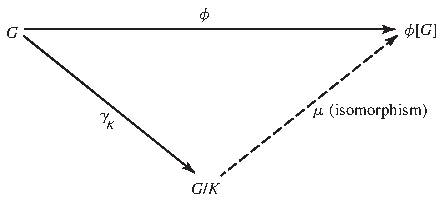
\includegraphics[width=0.602\linewidth,height=.8\textheight,keepaspectratio]{assets/p134_11.pdf}\end{center}
\begin{center}\small\textbf{12.15 Figure}\end{center}
\end{BookFloat}

\end{BookBody}

% Source PDF page 135; original printed page 118
\BookSource{135}{118}
\BookNarrativetrue

\begin{BookBody}

\BookLabel{12.16 Example} Classify the group \BookInline{(\mathbb{Z}_{4}\times \mathbb{Z}_{2})/(\{0\}\times \mathbb{Z}_{2})} according to the fundamental theorem of finitely generated abelian groups (Theorem 9.12).

\BookLabel{\textit{Solution}} The projection map \BookInline{\pi _{1}:\mathbb{Z}_{4}\times \mathbb{Z}_{2}\to \mathbb{Z}_{4}} given by \BookInline{\pi _{1}(x,\allowbreak y)= x} is a homomorphism of \BookInline{\mathbb{Z}_{4}\times \mathbb{Z}_{2}} onto \BookInline{\mathbb{Z}_{4}} with kernel \BookInline{\{0\}\times \mathbb{Z}_{2}.} By Theorem 12.14, we know that the given factor group is isomorphic to \BookInline{\mathbb{Z}_{4}.}\BookEnd{\blacktriangle}

\BookTextHeading{\textbf{Normal Subgroups and Inner Automorphisms}  }

\noindent We derive some alternative characterizations of normal subgroups, which often provide us with an easier way to check normality than finding both the left and the right coset decompositions.

Suppose that \BookInline{H} is a subgroup of \BookInline{G} such that \BookInline{ghg^{- 1}\in H} for all \BookInline{g\in G} and all \BookInline{h\in H.} Then \BookInline{gHg^{- 1}= \{ghg^{- 1}\mid h\in H\}\subseteq H} for all \BookInline{g\in G.} We claim that actually \BookInline{gHg^{- 1}= H.} We must show that \BookInline{H\subseteq gHg^{- 1}} for all \BookInline{g\in G.} Let \BookInline{h\in H.} Replacing \BookInline{g} by \BookInline{g^{- 1}} in the relation \BookInline{ghg^{- 1}\in H,\allowbreak } we obtain \BookInline{g^{- 1}h(g^{- 1})^{- 1}= g^{- 1}hg= h_{1}} where \BookInline{h_{1}\in H.} Consequently, \BookInline{h= gh_{1}g^{- 1}\in gHg^{- 1},\allowbreak } and we are done.

Suppose that \BookInline{gH= Hg} for all \BookInline{g\in G.} Then \BookInline{gh= h_{1}g,\allowbreak } so \BookInline{ghg^{- 1}\in H} for all \BookInline{g\in G} and all \BookInline{h\in H.} By the preceding paragraph, this means that \BookInline{gHg^{- 1}= H} for all \BookInline{g\in G.} Conversely, if \BookInline{gHg^{- 1}= H} for all \BookInline{g\in G,\allowbreak } then \BookInline{ghg^{- 1}= h_{1}} so \BookInline{gh= h_{1}g\in Hg,\allowbreak } and \BookInline{gH\subseteq Hg.} But also\BookInline{,\allowbreak g^{- 1}Hg= H} giving \BookInline{g^{- 1}hg= h_{2},\allowbreak } so that \BookInline{hg= gh_{2}} and \BookInline{Hg\subseteq } \BookInline{gH.}

The comments after Definition 12.3 show that the kernel of any homomorphism is a normal subgroup of the domain. Also, Theorem 12.12 says that any normal subgroup is the kernel of some homomorphism.

We summarize our work as a theorem.

\BookLabel{12.17 Theorem} The following are four equivalent conditions for a subgroup \BookInline{H} of a group \BookInline{G} to be a \textit{normal} subgroup of \BookInline{G.}

\BookExercise{1.}{\BookInline{ghg^{- 1}\in H} for all \BookInline{g\in G} and \BookInline{h\in H.}}

\BookExercise{2.}{\BookInline{gHg^{- 1}= H} for all \BookInline{g\in G.}}

\BookExercise{3.}{There is a group homomorphism \BookInline{\phi:G\to G^{\prime }} such that Ker\BookInline{(\phi )= H.}}

\BookExercise{4.}{\BookInline{gH= Hg} for all \BookInline{g\in G.}}

\noindent Condition (2) of Theorem 12.17 is often taken as the definition of a normal subgroup \BookInline{H} of a group \BookInline{G.}\BookEnd{\blacklozenge}

\BookLabel{12.18 Example} Every subgroup \BookInline{H} of an abelian group \BookInline{G} is normal. We need only note that \BookInline{gh= hg} for all \BookInline{h\in H} and all \BookInline{g\in G,\allowbreak } so, of course\BookInline{,\allowbreak ghg^{- 1}= h\in H} for all \BookInline{g\in G} and all \BookInline{h\in H.}\BookEnd{\blacktriangle}

If \BookInline{G} is a group and \BookInline{g\in G,\allowbreak } then the map \BookInline{i_{g}:G\to G} defined by \BookInline{i_{g}(x)= gxg^{- 1}} is a group homomorphism since \BookInline{i_{g}(xy)= gxyg^{- 1}= gxg^{- 1}gyg^{- 1}= i_{g}(x)i_{g}(x).} We see that \BookInline{gag^{- 1}= gbg^{- 1}} if and only if \BookInline{a= b,\allowbreak } so \BookInline{i_{g}} is one-to-one. Since \BookInline{g(g^{- 1}yg)g^{- 1}= y,\allowbreak } we see that \BookInline{i_{g}} is onto \BookInline{G,\allowbreak } so it is an isomorphism of \BookInline{G} with itself.

\BookLabel{12.19 Definition} An isomorphism \BookInline{\phi:G\to G} of a group \BookInline{G} with itself is an\textbf{ automorphism} of \BookInline{G.} The automorphism \BookInline{i_{g}:G\to G,\allowbreak } where \BookInline{i_{g}(x)= gxg^{- 1}} for all \BookInline{x\in G,\allowbreak } is the\textbf{ inner automor}\textbf{phism of} \BookInline{G} \textbf{by} \BookInline{g.} Performing \BookInline{i_{g}} on \BookInline{x} is called\textbf{ conjugation of} \BookInline{x} \textbf{by} \BookInline{g.}\BookEnd{\blacksquare}

The equivalence of conditions (1) and (2) in Theorem 12.17 shows that \BookInline{gH= Hg} for all \BookInline{g\in G} if and only if \BookInline{i_{g}[H]= H} for all \BookInline{g\in G,\allowbreak } that is, if and only if \BookInline{H} is\textbf{ invariant} under all inner automorphisms of \BookInline{G.} It is important to realize that \BookInline{i_{g}[H]= H} is an 
% Source PDF page 136; original printed page 119
\BookSource{136}{119}
equation in\textit{ sets;} we need not have \BookInline{i_{g}(h)= h} for all \BookInline{h\in H.} That is \BookInline{i_{g}} may perform a nontrivial\textit{ permutation} of the set \BookInline{H.} We see that the normal subgroups of a group \BookInline{G} are precisely those that are invariant under all inner automorphisms. A subgroup \BookInline{K} of \BookInline{G} is a\textbf{ conjugate subgroup} of \BookInline{H} if \BookInline{K= i_{g}[H]= gHg^{- 1}} for some \BookInline{g\in G.}

\end{BookBody}

\BookNarrativetrue

\begin{BookBody}

\end{BookBody}

\BookNarrativefalse

\begin{BookBody}

\BookExerciseTitle{12}

\BookTextHeading{\textbf{Computations}}

\noindent In Exercises 1 through 8, find the order of the given factor group.

\BookExercise{1.}{\BookInline{\mathbb{Z}_{6}/\langle 3\rangle }}

\BookExercise{2.}{\BookInline{(\mathbb{Z}_{4}\times \mathbb{Z}_{12})/(\langle 2\rangle \times \langle 2\rangle )}}

\BookExercise{3.}{\BookInline{(\mathbb{Z}_{4}\times \mathbb{Z}_{2})/\langle (2,\allowbreak 1)\rangle }}

\BookExercise{4.}{\BookInline{(\mathbb{Z}_{3}\times \mathbb{Z}_{5})/(\{0\}\times \mathbb{Z}_{5})}}

\BookExercise{5.}{\BookInline{(\mathbb{Z}_{3}\times \mathbb{Z}_{6})/\langle (1,\allowbreak 1)\rangle }}

\BookExercise{6.}{\BookInline{(\mathbb{Z}_{50}\times \mathbb{Z}_{75})/\langle (15,\allowbreak 15)\rangle }}

\BookExercise{7.}{\BookInline{(\mathbb{Z}_{26}\times \mathbb{Z}_{15})/\langle (1,\allowbreak 1)\rangle }}

\BookExercise{8.}{\BookInline{(\mathbb{Z}_{8}\times S_{3})/\langle (2,\allowbreak (1,\allowbreak 2,\allowbreak 3))\rangle } In Exercises 9 through 15, give the order of the element in the factor group.}

\BookExercise{9.}{\BookInline{5+ \langle 4\rangle } in \BookInline{\mathbb{Z}_{12}/\langle 4\rangle }}

\BookExercise{10.}{\BookInline{26+ \langle 12\rangle } in \BookInline{\mathbb{Z}_{60}/\langle 12\rangle }}

\BookExercise{11.}{\BookInline{(2,\allowbreak 1)+ \langle (1,\allowbreak 1)\rangle } in \BookInline{(\mathbb{Z}_{3}\times \mathbb{Z}_{6})/\langle (1,\allowbreak 1)\rangle }}

\BookExercise{12.}{\BookInline{(3,\allowbreak 1)+ \langle (1,\allowbreak 1)\rangle } in \BookInline{(\mathbb{Z}_{4}\times \mathbb{Z}_{4})/\langle (1,\allowbreak 1)\rangle }}

\BookExercise{13.}{\BookInline{(2,\allowbreak 3)+ \langle (0,\allowbreak 3)\rangle } in \BookInline{(\mathbb{Z}_{10}\times \mathbb{Z}_{4})/\langle (0,\allowbreak 3)\rangle }}

\BookExercise{14.}{\BookInline{(2,\allowbreak 5)+ \langle (1,\allowbreak 2)\rangle } in \BookInline{(\mathbb{Z}_{3}\times \mathbb{Z}_{6})/\langle (1,\allowbreak 2)\rangle }}

\BookExercise{15.}{\BookInline{(2,\allowbreak 0)+ \langle (4,\allowbreak 4)\rangle } in \BookInline{(\mathbb{Z}_{6}\times \mathbb{Z}_{8})/\langle (4,\allowbreak 4)\rangle }}

\BookExercise{16.}{Compute \BookInline{i_{\rho }[H]} for the subgroup \BookInline{H= \{\iota,\allowbreak \mu \}} of the dihedral group \BookInline{D_{3}.}}

\BookTextHeading{\textbf{Concepts}}

\noindent In Exercises 17 through 19, correct the definition of the italicized term without reference to the text, if correction is needed, so that it is in a form acceptable for publication.

\BookExercise{17.}{A\textit{ normal subgroup} \BookInline{H} of \BookInline{G} is one satisfying \BookInline{hG= Gh} for all \BookInline{h\in H.}}

\BookExercise{18.}{A\textit{ normal subgroup} \BookInline{H} of \BookInline{G} is one satisfying \BookInline{g^{- 1}hg\in H} for all \BookInline{h\in H} and all \BookInline{g\in G.}}

\BookExercise{19.}{An\textit{ automorphism} of a group \BookInline{G} is a homomorphism mapping \BookInline{G} into \BookInline{G.}}

\BookExercise{20.}{What is the importance of a\textit{ normal} subgroup of a group \BookInline{G}?}

\noindent Students often write nonsense when first proving theorems about factor groups. The next two exercises are designed to call attention to one basic type of error.

\BookExercise{21.}{A student is asked to show that if \BookInline{H} is a normal subgroup of an abelian group \BookInline{G,\allowbreak } then \BookInline{G/H} is abelian. The student’s proof starts as follows:}

\noindent We must show that \BookInline{G/H} is abelian. Let \BookInline{a} and \BookInline{b} be two elements of \BookInline{G/H.}

\BookExercise{a.}{Why does the instructor reading this proof expect to find nonsense from here on in the student’s paper?}

\BookExercise{b.}{What should the student have written?}

\BookExercise{c.}{Complete the proof.}

\BookExercise{22.}{A\textbf{ torsion group} is a group all of whose elements have finite order. A group is\textbf{ torsion free} if the identity is the only element of finite order. A student is asked to prove that if \BookInline{G} is a torsion group, then so is \BookInline{G/H} for every normal subgroup \BookInline{H} of \BookInline{G.} The student writes}

\noindent We must show that each element of \BookInline{G/H} is of finite order. Let \BookInline{x\in G/H.} Answer the same questions as in Exercise 21.

\BookExercise{23.}{Determine whether each of the following is true or false.}

\BookExercise{a.}{It makes sense to speak of the factor group \BookInline{G/N} if and only if \BookInline{N} is a normal subgroup of the group \BookInline{G.}}

\BookExercise{b.}{Every subgroup of an abelian group \BookInline{G} is a normal subgroup of \BookInline{G.}}

\BookExercise{c.}{The only automorphism of an abelian group is the identity map.}

\end{BookBody}

% Source PDF page 137; original printed page 120
\BookSource{137}{120}
\BookNarrativefalse

\begin{BookBody}

\BookExercise{d.}{Every factor group of a finite group is again of finite order.}

\BookExercise{e.}{Every factor group of a torsion group is a torsion group. (See Exercise 22.)}

\BookExercise{f.}{Every factor group of a torsion-free group is torsion free. (See Exercise 22.)}

\BookExercise{g.}{Every factor group of an abelian group is abelian.}

\BookExercise{h.}{Every factor group of a nonabelian group is nonabelian.}

\BookExercise{i.}{\textbf{i}\BookInline{.\mathbb{Z}/n\mathbb{Z}} is cyclic of order \BookInline{n.}}

\BookExercise{j.}{\textbf{j}\BookInline{.\mathbb{R}/n\mathbb{R}} is cyclic of order \BookInline{n,\allowbreak } where \BookInline{n\mathbb{R}= \{nr\mid r\in \mathbb{R}\}} and \BookInline{\mathbb{R}} is under addition.}

\BookTextHeading{\textbf{Theory}}

\BookExercise{24.}{Let \BookInline{G_{1}} and \BookInline{G_{2}} be groups and \BookInline{\pi _{1}:G_{1}\times G_{2}\to G_{1}} be the function defined by \BookInline{\pi _{1}(a,\allowbreak b)= a.} Prove that \BookInline{\pi _{1}} is a homomorphism, find Ker\BookInline{(\pi _{1}),\allowbreak } and prove \BookInline{(G_{1}\times G_{2})/}Ker\BookInline{(\pi _{1})} is isomorphic to \BookInline{G_{1}.}}

\BookExercise{25.}{Let \BookInline{G_{1}} and \BookInline{G_{2}} be groups and \BookInline{\phi:G_{1}\times G_{2}\to G_{1}\times G_{2}} be the function defined by \BookInline{\phi (a,\allowbreak b)= (a,\allowbreak e_{2})} where \BookInline{e_{2}} is the identity in \BookInline{G_{2}.} Prove that \BookInline{\phi } is a homomorphism, find Ker\BookInline{(\phi ),\allowbreak } and prove \BookInline{(G_{1}\times G_{2})/}Ker\BookInline{(\phi )} is isomorphic to \BookInline{G_{1}.}}

\BookExercise{26.}{Complete the proof of Theorem 12.7 by showing that if \BookInline{H} is a subgroup of a group \BookInline{G} and if left coset multiplication \BookInline{(aH)(bH)= (ab)H} is well defined, then \BookInline{Ha\subseteq aH.}}

\BookExercise{27.}{Prove that the torsion subgroup \BookInline{T} of an abelian group \BookInline{G} is a normal subgroup of \BookInline{G,\allowbreak } and that \BookInline{G/T} is torsion free. (See Exercise 22.)}

\BookExercise{28.}{A subgroup \BookInline{H} is\textbf{ conjugate to a subgroup} \BookInline{K} of a group \BookInline{G} if there exists an inner automorphism \BookInline{i_{g}} of \BookInline{G} such that \BookInline{i_{g}[H]= K.} Show that conjugacy is an equivalence relation on the collection of subgroups of \BookInline{G.}}

\BookExercise{29.}{Characterize the normal subgroups of a group \BookInline{G} in terms of the cells where they appear in the partition given by the conjugacy relation in the preceding exercise.}

\BookExercise{30.}{Find all subgroups of \BookInline{D_{3}} that are conjugate to \BookInline{H= \{\iota,\allowbreak \mu \}.(}See Exercise 28.)}

\BookExercise{31.}{\textbf{ (Evaluation Homomorphism)} Let \BookInline{F} be the set of all functions mapping the real numbers to the real numbers and let \BookInline{c\in \mathbb{R}.} The sum of two functions \BookInline{f+ g} is the function defined by \BookInline{(f+ g)(x)= f(x)+ g(x).} Function addition makes \BookInline{F} a group. Let \BookInline{\phi _{c}:F\to \mathbb{R}} be defined by \BookInline{\phi _{c}(f)= f(c).}}

\BookExercise{a.}{Show that \BookInline{\phi _{c}} is a group homomorphism.}

\BookExercise{b.}{Find Ker\BookInline{(\phi _{c}).}}

\BookExercise{c.}{Identify the coset of Ker\BookInline{(\phi _{c})} that contains the constant function \BookInline{f(x)= 1.}}

\BookExercise{d.}{Find a well-known group that is isomorphic with \BookInline{F/}Ker\BookInline{(\phi _{c}).} Use the Fundamental Homomorphism Theorem to prove your answer.}

\BookExercise{32.}{Let \BookInline{H} be a normal subgroup of a group \BookInline{G,\allowbreak } and let \BookInline{m= (G:H).} Show that \BookInline{a^{m}\in H} for every \BookInline{a\in G.}}

\BookExercise{33.}{Show that an intersection of normal subgroups of a group \BookInline{G} is again a normal subgroup of \BookInline{G.}}

\BookExercise{34.}{Given any subset \BookInline{S} of a group \BookInline{G,\allowbreak } show that it makes sense to speak of the smallest normal subgroup that contains \BookInline{S.[}\textit{Hint:} Use Exercise 33.]}

\BookExercise{35.}{Let \BookInline{G} be a group. An element of \BookInline{G} that can be expressed in the form \BookInline{aba^{- 1}b^{- 1}} for some \BookInline{a,\allowbreak b\in G} is a \textbf{commutator} in \BookInline{G.} The preceding exercise shows that there is a smallest normal subgroup \BookInline{C} of a group \BookInline{G} containing all commutators in \BookInline{G;} the subgroup \BookInline{C} is the\textbf{ commutator subgroup} of \BookInline{G.} Show that \BookInline{G/C} is an abelian group.}

\BookExercise{36.}{Show that if a finite group \BookInline{G} has exactly one subgroup \BookInline{H} of a given order, then \BookInline{H} is a normal subgroup of \BookInline{G.}}

\BookExercise{37.}{Show that if \BookInline{H} and \BookInline{N} are subgroups of a group \BookInline{G,\allowbreak } and \BookInline{N} is normal in \BookInline{G,\allowbreak } then \BookInline{H\cap N} is normal in \BookInline{H.} Show by an example that \BookInline{H\cap N} need not be normal in \BookInline{G.}}

\BookExercise{38.}{Let \BookInline{G} be a group containing at least one subgroup of a fixed finite order \BookInline{s.} Show that the intersection of all subgroups of \BookInline{G} of order \BookInline{s} is a normal subgroup of \BookInline{G.[}\textit{Hint:} Use the fact that if \BookInline{H} has order \BookInline{s,\allowbreak } then so does \BookInline{x^{- 1}Hx} for all \BookInline{x\in G.]}}

\end{BookBody}

% Continuation on source PDF page 138, preceding Section 13
\BookNarrativefalse

\begin{BookBody}

\BookExercise{39.}{\textbf{. a} Show that all automorphisms of a group \BookInline{G} form a group under function composition.}

\BookExercise{b.}{Show that the inner automorphisms of a group \BookInline{G} form a normal subgroup of the group of all automorphisms of \BookInline{G} under function composition. [\textit{Warning:} Be sure to show that the inner automorphisms do form a subgroup.]}

\BookExercise{40.}{Show that the set of all \BookInline{g\in G} such that \BookInline{i_{g}:G\to G} is the identity inner automorphism \BookInline{i_{e}} is a normal subgroup of a group \BookInline{G.}}

\BookExercise{41.}{Let \BookInline{G} and \BookInline{G^{\prime }} be groups, and let \BookInline{H} and \BookInline{H^{\prime }} be normal subgroups of \BookInline{G} and \BookInline{G^{\prime },\allowbreak } respectively. Let \BookInline{\phi } be a homomorphism of \BookInline{G} into \BookInline{G^{\prime }.} Show that \BookInline{\phi } induces a natural homomorphism \BookInline{\phi _{\ast }:(G/H)\to (G^{\prime }/H^{\prime })} if \BookInline{\phi [H]\subseteq H^{\prime }.} (This fact is used constantly in algebraic topology.)}

\BookExercise{42.}{Use the properties det\BookInline{(AB)= } det\BookInline{(A)\cdot } det\BookInline{(B)} and det\BookInline{(I_{n})= 1} for \BookInline{n\times n} matrices to show the \BookInline{n\times n} matrices with determinant \BookInline{\pm 1} form a normal subgroup of GL\BookInline{(n,\allowbreak \mathbb{R}).}}

\BookExercise{43.}{Let \BookInline{G} be a group, and let \BookInline{\mathcal{P}(G)} be the set of all\textit{ subsets} of \BookInline{G.} For any \BookInline{A,\allowbreak B\in \mathcal{P}(G),\allowbreak } let us define the product subset \BookInline{AB= \{ab\mid a\in A,\allowbreak b\in B\}.}}

\BookExercise{a.}{Show that this multiplication of subsets is associative and has an identity element, but that \BookInline{\mathcal{P}(G)} is not a group under this operation.}

\BookExercise{b.}{Show that if \BookInline{N} is a normal subgroup of \BookInline{G,\allowbreak } then the set of cosets of \BookInline{N} is closed under the above operation on \BookInline{\mathcal{P}(G),\allowbreak } and that this operation agrees with the multiplication given by the formula in Corollary 12.8.}

\BookExercise{c.}{Show (without using Corollary 12.8) that the cosets of \BookInline{N} in \BookInline{G} form a group under the above operation. Is its identity element the same as the identity element of \BookInline{\mathcal{P}(G)}?}

\end{BookBody}
\ifdefined\BookMaster\let\BookFinish\relax\else\def\BookFinish{\end{document}}\fi\BookFinish

\clearpage
% !TeX program = xelatex
\ifdefined\BookMaster\else
\documentclass[11pt,oneside]{article}
% !TeX program = xelatex
\usepackage[b5paper,left=22mm,right=22mm,top=20mm,bottom=22mm,footskip=11mm]{geometry}
\usepackage{fontspec}
\setmainfont{TeX Gyre Termes}
\setsansfont{TeX Gyre Heros}
\usepackage{amsmath,amssymb,mathtools,amsthm}
\renewcommand{\cdots}{\mathinner{\cdotp\cdotp\cdotp}}
\usepackage{graphicx,adjustbox,array,booktabs,longtable,multirow,enumitem,changepage,needspace}
\usepackage[table]{xcolor}
\usepackage{fancyhdr}
\raggedbottom
\interfootnotelinepenalty=10000
\newcommand{\BookFootnote}[2]{\begingroup\renewcommand{\thefootnote}{\fnsymbol{footnote}}\footnote[#1]{#2}\endgroup}
\newcommand{\BookFootnoteMark}[1]{\begingroup\renewcommand{\thefootnote}{\fnsymbol{footnote}}\footnotemark[#1]\endgroup}
\newcommand{\BookFootnoteText}[2]{\begingroup\renewcommand{\thefootnote}{\fnsymbol{footnote}}\footnotetext[#1]{#2}\endgroup}
\newenvironment{BookFloat}[1]{\par\addvspace{.6\baselineskip}\noindent\def\BookFloatID{#1}\begin{minipage}{\linewidth}\phantomsection\label{bookfloat:#1:start}}{\phantomsection\label{bookfloat:\BookFloatID:end}\end{minipage}\par\addvspace{.6\baselineskip}}

\usepackage[unicode,hidelinks]{hyperref}
\pagestyle{fancy}
\fancyhf{}
\newcommand{\BookFooter}{}
\fancyfoot[L]{\parbox[b]{\dimexpr\textwidth-15mm}{\footnotesize\BookFooter}}
\fancyfoot[R]{\footnotesize\thepage}
\renewcommand{\headrulewidth}{0pt}
\renewcommand{\footrulewidth}{0pt}
\setlength{\parindent}{0pt}
\setlength{\parskip}{0.2em}
\setlength{\emergencystretch}{3em}
\setlist{nosep,leftmargin=1.7em,labelsep=.65em}
\newif\ifBookNarrative
\BookNarrativetrue
\newenvironment{BookBody}{\setlength{\parindent}{0pt}}{}
\newcommand{\BookStatement}[1]{\par\addvspace{.6\baselineskip}\noindent #1\enspace\ignorespaces}
\newcommand{\BookLabel}[1]{\par\addvspace{.6\baselineskip}\needspace{3\baselineskip}\noindent\textbf{#1}\quad\ignorespaces}
\newcommand{\BookHeading}[1]{\par\addvspace{\baselineskip}\needspace{4\baselineskip}\noindent{\large\bfseries #1}\par\medskip}
\newcommand{\BookSubheading}[1]{\par\addvspace{.7\baselineskip}\needspace{3\baselineskip}\noindent{\bfseries #1}\par\smallskip}
\newcommand{\BookTextHeading}[1]{\par\addvspace{.7\baselineskip}\needspace{3\baselineskip}\noindent #1\par\smallskip}
\newcommand{\BookSectionTitle}[2]{\par\addvspace{1.2\baselineskip}\needspace{5\baselineskip}\noindent\colorbox{gray!25}{\sffamily\bfseries\small SECTION #1}\quad{\large\bfseries #2}\par\medskip}
\newcommand{\BookExerciseTitle}[1]{\par\addvspace{\baselineskip}\needspace{4\baselineskip}\noindent{\color{gray}\rule{1.5mm}{1.5mm}}\enspace{\large\bfseries Exercises #1}\par\medskip}
\newcommand{\BookBullet}[1]{\begin{list}{\textbullet}{\setlength{\leftmargin}{1.7em}\setlength{\labelwidth}{1em}\setlength{\labelsep}{.7em}\setlength{\topsep}{0pt}\setlength{\parsep}{0pt}\setlength{\itemsep}{0pt}}\item #1\end{list}}
\newcommand{\BookExercise}[2]{\begin{list}{\textbf{#1}}{\setlength{\leftmargin}{2.2em}\setlength{\labelwidth}{1.5em}\setlength{\labelsep}{.7em}\setlength{\topsep}{.15em}\setlength{\parsep}{0pt}\setlength{\itemsep}{0pt}}\item #2\end{list}}
\newcommand{\BookEnd}[1]{\unskip\nobreak\hfill\ensuremath{#1}}
\newcommand{\BookSource}[2]{\phantomsection\label{sourcepage:#1}} % Source-page anchors, retained through reflow.
\usepackage{multicol}
\usepackage{tikz}
\newcommand{\BookPartEntry}[2]{\par\noindent\makebox[17mm][l]{\bfseries Section #1}#2\par}
\newcommand{\BookPartTitle}[3]{\par\bigskip\noindent\begin{tikzpicture}\node[anchor=north west,inner sep=0pt,outer sep=0pt] (bookpart) at (0,0) {\begin{minipage}{\dimexpr\linewidth-.5pt}\hspace*{26mm}\begin{minipage}[t]{\dimexpr\linewidth-26mm}\begin{adjustbox}{max width=\linewidth}{\fontsize{20}{24}\selectfont\bfseries #2}\end{adjustbox}\par\vspace{6mm}\hrule\vspace{6mm}{\sffamily\footnotesize\setlength{\parskip}{.3em}#3}\vspace{3mm}\end{minipage}\end{minipage}};\path[shade,top color=gray!60,bottom color=white] (0,0) rectangle ([xshift=24mm]bookpart.south west);\node[anchor=north,font=\sffamily\bfseries\small] at (12mm,-2mm) {PART};\node[anchor=north,font=\sffamily\bfseries\Huge] at (12mm,-7mm) {#1};\end{tikzpicture}\par\bigskip}
\newsavebox{\BookMathBox}
\makeatletter
\newcommand{\BookInline}[1]{\leavevmode\hskip0pt\relax\begingroup\in@{\begin}{#1}\ifin@\sbox{\BookMathBox}{\(#1\)}\ifdim\wd\BookMathBox>\dimexpr\linewidth-1em\relax\resizebox{\dimexpr\linewidth-1em\relax}{!}{\usebox{\BookMathBox}}\else\(#1\)\fi\else\in@{\left}{#1}\ifin@\sbox{\BookMathBox}{\(#1\)}\ifdim\wd\BookMathBox>\dimexpr\linewidth-1em\relax\resizebox{\dimexpr\linewidth-1em\relax}{!}{\usebox{\BookMathBox}}\else\(#1\)\fi\else\(#1\)\fi\fi\endgroup\hskip0pt\relax}
\makeatother
\DeclareMathOperator{\Aut}{Aut}
\DeclareMathOperator{\End}{End}
\DeclareMathOperator{\Hom}{Hom}
\DeclareMathOperator{\GF}{GF}
\DeclareMathOperator{\irr}{irr}
\DeclareMathOperator{\lt}{lt}
\DeclareMathOperator{\lp}{lp}
\providecommand{\textcircled}[1]{\textnormal{(#1)}}

\begin{document}
\fi
\renewcommand{\BookFooter}{Section 13 Factor-Group Computations and Simple Groups}
\pdfbookmark[0]{Section 13 Factor-Group Computations and Simple Groups}{13_factor_group_computations_and_simple_groups}
\ifdefined\BookMaster\else\setcounter{page}{121}\fi
% Source PDF page 138; original printed page 121
\BookSource{138}{121}
\BookNarrativetrue

\begin{BookBody}

\BookSectionTitle{13}{Factor-Group Computations and Simple Groups}

\noindent Factor groups can be a tough topic for students to grasp. There is nothing like a bit of computation to strengthen understanding in mathematics. We start by attempting to improve our intuition concerning factor groups. Since we will be dealing with normal subgroups throughout this section, we often denote a subgroup of a group \BookInline{G} by \BookInline{N} rather than by \BookInline{H.}

Let \BookInline{N} be a normal subgroup of \BookInline{G.} In the factor group \BookInline{G/N,\allowbreak } the subgroup \BookInline{N} acts as identity element. We may regard \BookInline{N} as being\textit{ collapsed} to a single element, either to 0 in additive notation or to \BookInline{e} in multiplicative notation. This collapsing of \BookInline{N} together with the algebraic structure of \BookInline{G} require that other subsets of \BookInline{G,\allowbreak } namely, the cosets of \BookInline{N,\allowbreak } also each collapse into a single element in the factor group. A visualization of this collapsing is provided by Fig. 13.1. Recall from Theorem 12.12 that \BookInline{\gamma:G\to G/N} defined by \BookInline{\gamma (a)= } \textit{aN} for \BookInline{a\in G} is a homomorphism of \BookInline{G} onto \BookInline{G/N.} We can view the “line” \BookInline{G/N} at the bottom of Figure 13.1 as obtained by collapsing to a point each coset of \BookInline{N} in a copy of \BookInline{G.} Each point of \BookInline{G/N} thus corresponds to a whole vertical line

\begin{BookFloat}{13_factor_group_computations_and_simple_groups-p138-3}
\begin{center}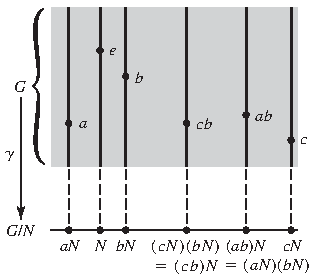
\includegraphics[width=0.429\linewidth,height=.8\textheight,keepaspectratio]{assets/p138_12.pdf}\end{center}
\begin{center}\small\textbf{13.1 Figure}\end{center}
\end{BookFloat}

\end{BookBody}

% Source PDF page 139; original printed page 122
\BookSource{139}{122}
\BookNarrativetrue

\begin{BookBody}

\noindent segment in the shaded portion, representing a coset of \BookInline{N} in \BookInline{G.} It is crucial to remember that multiplication of cosets in \BookInline{G/N} can be computed by multiplying in \BookInline{G,\allowbreak } using any representative elements of the cosets as shown in the figure.

Additively, two elements of \BookInline{G} will collapse into the same element of \BookInline{G/N} if they differ by an element of \BookInline{N.} Multiplicatively\BookInline{,\allowbreak a} and \BookInline{b} collapse together if \BookInline{ab^{- 1}} is in \BookInline{N.} The degree of collapsing can vary from nonexistent to catastrophic. We illustrate the two extreme cases by examples.

\BookLabel{13.2 Example} The trivial subgroup \BookInline{N= \{0\}} of \BookInline{\mathbb{Z}} is, of course, a normal subgroup. Compute \BookInline{\mathbb{Z}/\{0\}.}

\BookLabel{\textit{Solution}} Since \BookInline{N= \{0\}} has only one element, every coset of \BookInline{N} has only one element. That is, the cosets are of the form \BookInline{\{m\}} for \BookInline{m\in \mathbb{Z}.} There is no collapsing at all, and consequently, \BookInline{\mathbb{Z}/\{0\}\simeq \mathbb{Z}.} Each \BookInline{m\in \mathbb{Z}} is simply renamed \BookInline{\{m\}} in \BookInline{\mathbb{Z}/\{0\}.}\BookEnd{\blacktriangle}

\BookLabel{13.3 Example} Let \BookInline{n} be a positive integer. The set \BookInline{n\mathbb{R}= \{nr\mid r\in \mathbb{R}\}} is a subgroup of \BookInline{\mathbb{R}} under addition, and it is normal since \BookInline{\mathbb{R}} is abelian. Compute \BookInline{\mathbb{R}/n\mathbb{R}.}

\BookLabel{\textit{Solution}} A bit of thought shows that actually \BookInline{n\mathbb{R}= \mathbb{R},\allowbreak } because each \BookInline{x\in \mathbb{R}} is of the form \BookInline{n(x/n)} and \BookInline{x/n\in \mathbb{R}.} Thus \BookInline{\mathbb{R}/n\mathbb{R}} has only one element, the subgroup \BookInline{n\mathbb{R}.} The factor group is a trivial group consisting only of the identity element\BookInline{.}\BookEnd{\blacktriangle}

As illustrated in Examples 13.2 and 13.3 for any group \BookInline{G,\allowbreak } we have \BookInline{G/\{e\}\simeq G} and \BookInline{G/G\simeq \{e\},\allowbreak } where \BookInline{\{e\}} is the trivial group consisting only of the identity element \BookInline{e.} These two extremes of factor groups are of little importance. We would like knowledge of a factor group \BookInline{G/N} to give some information about the structure of \BookInline{G.} If \BookInline{N= \{e\},\allowbreak } the factor group has the same structure as \BookInline{G} and we might as well have tried to study \BookInline{G} directly. If \BookInline{N= G,\allowbreak } the factor group has no significant structure to supply information about \BookInline{G.} If \BookInline{G} is a finite group and \BookInline{N\neq \{e\}} is a normal subgroup of \BookInline{G,\allowbreak } then \BookInline{G/N} is a smaller group than \BookInline{G,\allowbreak } and consequently may have a more simple structure than \BookInline{G.} The multiplication of cosets in \BookInline{G/N} reflects the multiplication in \BookInline{G,\allowbreak } since products of cosets can be computed by multiplying in \BookInline{G} representative elements of the cosets.

We give two examples showing that even when \BookInline{G/N} has order 2, we may be able to deduce some useful results. If \BookInline{G} is a finite group and \BookInline{G/N} has just two elements, then we must have \BookInline{|G|= 2|N|.} Note that every subgroup \BookInline{H} containing just half the elements of a finite group \BookInline{G} must be a normal subgroup, since for each element \BookInline{a} in \BookInline{G} but not in \BookInline{H,\allowbreak } both the left coset \BookInline{aH} and the right coset \BookInline{Ha} must consist of all elements in \BookInline{G} that are not in \BookInline{H.} Thus the left and right cosets of \BookInline{H} coincide and \BookInline{H} is a normal subgroup of \BookInline{G.}

\BookLabel{13.4 Example} Because \BookInline{|S_{n}|= 2|A_{n}|,\allowbreak } we see that \BookInline{A_{n}} is a normal subgroup of \BookInline{S_{n},\allowbreak } and \BookInline{S_{n}/A_{n}} has order 2. Let \BookInline{\sigma } be an odd permutation in \BookInline{S_{n},\allowbreak } so that \BookInline{S_{n}/A_{n}= \{A_{n},\allowbreak \sigma A_{n}\}.} Renaming the element \BookInline{A_{n}} “even” and the element \BookInline{\sigma A_{n}} “odd,” the multiplication in \BookInline{S_{n}/A_{n}} shown in Table 13.5 becomes

\begin{center}\begin{adjustbox}{max width=\linewidth}\BookInline{\displaystyle \begin{aligned}(\;\text{even}\;)(\;\text{even}\;)&= \;\text{even}\;(\;\text{odd}\;)(\;\text{even}\;)= \;\text{odd}\; \\ (\;\text{even}\;)(\;\text{odd}\;)&= \;\text{odd}\;(\;\text{odd}\;)(\;\text{odd}\;)= \;\text{even}\;.\end{aligned}}\end{adjustbox}\end{center}

\begin{BookFloat}{13_factor_group_computations_and_simple_groups-p139-10}
\begin{center}\small\textbf{13.5 Table}\end{center}
\begin{center}\begin{adjustbox}{max width=\linewidth}
\renewcommand{\arraystretch}{1.2}\setlength{\tabcolsep}{5pt}
\begin{tabular}{c|c|c}
 & \BookInline{A_{n}} & \BookInline{\sigma A_{n}}\\\hline
\BookInline{A_{n}} & \BookInline{A_{n}} & \BookInline{\sigma A_{n}}\\\hline
\BookInline{\sigma A_{n}} & \BookInline{\sigma A_{n}} & \BookInline{A_{n}}\\
\end{tabular}
\end{adjustbox}\end{center}
\end{BookFloat}

\noindent Thus the factor group reflects these multiplicative properties for all the permutations in \BookInline{S_{n}.}\BookEnd{\blacktriangle}

Example 13.4 illustrates that while knowing the product of two cosets in \BookInline{G/N} does not tell us what the product of two elements of \BookInline{G} is, it may tell us that the product in \BookInline{G} of two\textit{ types} of elements is itself of a certain type.

\end{BookBody}

% Source PDF page 140; original printed page 123
\BookSource{140}{123}
\BookNarrativetrue

\begin{BookBody}

\BookLabel{13.6 Example} \textbf{(The Converse of the Theorem of Lagrange is False)} Recall that the Theorem of Lagrange states that the order of a subgroup of a finite group \BookInline{G} must divide the order of \BookInline{G.} We are now in a position to demonstrate that although the group \BookInline{A_{4}} has 12 elements and 6 divides \BookInline{12,\allowbreak A_{4}} has no subgroup of order 6.

Suppose that \BookInline{H} were a subgroup of \BookInline{A_{4}} having order 6. As observed before in Example 13.4, it would follow that \BookInline{H} would be a normal subgroup of \BookInline{A_{4}.} Then \BookInline{A_{4}/H} would have only two elements\BookInline{,\allowbreak H} and \BookInline{\sigma H} for some \BookInline{\sigma \in A_{4}} not in \BookInline{H.} Since in a group of order 2, the square of each element is the identity, we would have \BookInline{HH= H} and \BookInline{(\sigma H)(\sigma H)= H.} Now computation in a factor group can be achieved by computing with representatives in the original group. Thus, computing in \BookInline{A_{4},\allowbreak } we find that for each \BookInline{\alpha \in H} we must have \BookInline{\alpha ^{2}\in H} and for each \BookInline{\beta \in \sigma H} we must have \BookInline{\beta ^{2}\in H.} That is, the square of every element in \BookInline{A_{4}} must be in \BookInline{H.} But in \BookInline{A_{4},\allowbreak } we have

\begin{center}\begin{adjustbox}{max width=\linewidth}\BookInline{\displaystyle (1,\allowbreak 2,\allowbreak 3)= (1,\allowbreak 3,\allowbreak 2)^{2}\;\text{and}\;(1,\allowbreak 3,\allowbreak 2)= (1,\allowbreak 2,\allowbreak 3)^{2}}\end{adjustbox}\end{center}

\noindent so (1, 2, 3) and (1, 3, 2) are in \BookInline{H.} A similar computation shows that (1, 2, 4), (1, 4, 2), (1, 3, 4), (1, 4, 3), (2, 3, 4), and (2, 4, 3) are all in \BookInline{H.} This shows that there must be at least 8 elements in \BookInline{H,\allowbreak } contradicting the fact that \BookInline{H} was supposed to have order \BookInline{6.}\BookEnd{\blacktriangle}

We now turn to several examples that\textit{ compute} factor groups. If the group we start with is finitely generated and abelian, then its factor group will be also.\textit{ Computing} such a factor group means classifying it according to the fundamental theorem (Theorem 9.12 or Theorem 9.14).

\BookLabel{13.7 Example} Let us compute the factor group \BookInline{(\mathbb{Z}_{4}\times \mathbb{Z}_{6})/\langle (0,\allowbreak 1)\rangle.} Here \BookInline{\langle (0,\allowbreak 1)\rangle } is the cyclic subgroup \BookInline{H} of \BookInline{\mathbb{Z}_{4}\times \mathbb{Z}_{6}} generated by (0, 1). Thus

\begin{center}\begin{adjustbox}{max width=\linewidth}\BookInline{\displaystyle H= \{(0,\allowbreak 0),\allowbreak (0,\allowbreak 1),\allowbreak (0,\allowbreak 2),\allowbreak (0,\allowbreak 3),\allowbreak (0,\allowbreak 4),\allowbreak (0,\allowbreak 5)\}.}\end{adjustbox}\end{center}

\noindent Since \BookInline{\mathbb{Z}_{4}\times \mathbb{Z}_{6}} has 24 elements and \BookInline{H} has 6 elements, all cosets of \BookInline{H} must have 6 elements, and \BookInline{(\mathbb{Z}_{4}\times \mathbb{Z}_{6})/H} must have order 4. Since \BookInline{\mathbb{Z}_{4}\times \mathbb{Z}_{6}} is abelian, so is \BookInline{(\mathbb{Z}_{4}\times \mathbb{Z}_{6})/H(}remember, we compute in a factor group by means of representatives from the original group). In additive notation, the cosets are

\begin{center}\begin{adjustbox}{max width=\linewidth}\BookInline{\displaystyle H= (0,\allowbreak 0)+ H,\allowbreak (1,\allowbreak 0)+ H,\allowbreak (2,\allowbreak 0)+ H,\allowbreak (3,\allowbreak 0)+ H.}\end{adjustbox}\end{center}

\noindent Since we can compute by choosing the representatives (0, 0), (1, 0), (2, 0), and (3, 0), it is clear that \BookInline{(\mathbb{Z}_{4}\times \mathbb{Z}_{6})/H} is isomorphic to \BookInline{\mathbb{Z}_{4}.} Note that this is what we would expect, since in a factor group modulo \BookInline{H,\allowbreak } everything in \BookInline{H} becomes the identity element; that is, we are essentially setting everything in \BookInline{H} equal to zero. Thus the whole second factor \BookInline{\mathbb{Z}_{6}} of \BookInline{\mathbb{Z}_{4}\times \mathbb{Z}_{6}} is collapsed, leaving just the first factor \BookInline{\mathbb{Z}_{4}.}\BookEnd{\blacktriangle}

Example 13.7 is a special case of a general theorem that we now state and prove. We should acquire an intuitive feeling for this theorem in terms of\textit{ collapsing one of the} \textit{factors to the identity element}.

\BookLabel{13.8 Theorem} Let \BookInline{G= H\times K} be the direct product of groups \BookInline{H} and \BookInline{K.} Then \BookInline{H= \{(h,\allowbreak e)\mid h\in H\}} is a normal subgroup of \BookInline{G.} Also \BookInline{G/H} is isomorphic to \BookInline{K} in a natural way. Similarly, \BookInline{G/K\simeq H} in a natural way.

\BookLabel{\textit{Proof}} Consider the homomorphism \BookInline{\pi _{2}:H\times K\to K,\allowbreak } where \BookInline{\pi _{2}(h,\allowbreak k)= k.} Because Ker\BookInline{(\pi _{2})= } \BookInline{H,\allowbreak } we see that \BookInline{H} is a normal subgroup of \BookInline{H\times K.} Because \BookInline{\pi _{2}} is onto \BookInline{K,\allowbreak } Theorem 12.14 tells us that \BookInline{(H\times K)/H\simeq K.}\BookEnd{\blacklozenge}

We continue with additional computations of abelian factor groups. To illustrate how easy it is to compute in a factor group if we can compute in the whole group, we prove the following theorem.

\end{BookBody}

% Source PDF page 141; original printed page 124
\BookSource{141}{124}
\BookNarrativetrue

\begin{BookBody}

\BookLabel{13.9 Theorem} If \BookInline{G} is a cyclic group and \BookInline{N} is a subgroup of \BookInline{G,\allowbreak } then \BookInline{G/N} is cyclic.

\BookLabel{\textit{Proof}} Let \BookInline{G} be a cyclic group, so \BookInline{\langle a\rangle = G} for some \BookInline{a\in G.} Let \BookInline{N} be any subgroup of \BookInline{G.} Since \BookInline{G} is abelian\BookInline{,\allowbreak N} is a normal subgroup of \BookInline{G.} We compute the cyclic subgroup of \BookInline{G/N} generated by\textit{ aN}.

\begin{center}\begin{adjustbox}{max width=\linewidth}\BookInline{\displaystyle \langle aN\rangle = \{(aN)^{n}\mid n\in \mathbb{Z}\}= \{a^{n}N\mid n\in \mathbb{Z}\}}\end{adjustbox}\end{center}

\noindent Since \BookInline{\{a^{n}\mid n\in \mathbb{Z}\}= G,\allowbreak }

\begin{center}\begin{adjustbox}{max width=\linewidth}\BookInline{\displaystyle \{a^{n}N\mid n\in \mathbb{Z}\}= \{gN\mid g\in G\}.}\end{adjustbox}\end{center}

\noindent So \BookInline{\langle }\textit{aN}\BookInline{\rangle } contains every coset of \BookInline{G} and we see that \BookInline{G/N} is cyclic with generator \BookInline{\langle }\textit{aN}\BookInline{\rangle.} \BookEnd{\blacklozenge}

\BookLabel{13.10 Example} Let us compute the factor group \BookInline{(\mathbb{Z}_{4}\times \mathbb{Z}_{6})/\langle (0,\allowbreak 2)\rangle.} Now (0, 2) generates the subgroup

\begin{center}\begin{adjustbox}{max width=\linewidth}\BookInline{\displaystyle H= \{(0,\allowbreak 0),\allowbreak (0,\allowbreak 2),\allowbreak (0,\allowbreak 4)\}}\end{adjustbox}\end{center}

\noindent of \BookInline{\mathbb{Z}_{4}\times \mathbb{Z}_{6}} of order 3. Here the first factor \BookInline{\mathbb{Z}_{4}} of \BookInline{\mathbb{Z}_{4}\times \mathbb{Z}_{6}} is left alone. The \BookInline{\mathbb{Z}_{6}} factor, on the other hand, is essentially collapsed by a subgroup of order 3, giving a factor group in the second factor of order 2 that must be isomorphic to \BookInline{\mathbb{Z}_{2}.} Thus \BookInline{(\mathbb{Z}_{4}\times \mathbb{Z}_{6})/\langle (0,\allowbreak 2)\rangle } is isomorphic to \BookInline{\mathbb{Z}_{4}\times \mathbb{Z}_{2}.}

We can verify that \BookInline{(\mathbb{Z}_{4}\times \mathbb{Z}_{6})/\langle (0,\allowbreak 2)\rangle } is isomorphic to \BookInline{\mathbb{Z}_{4}\times \mathbb{Z}_{2}} by using Theorem 12.14. We need a homomorphism \BookInline{\phi:\mathbb{Z}_{4}\times \mathbb{Z}_{6}\to \mathbb{Z}_{4}\times \mathbb{Z}_{2}} that is onto, with kernel \BookInline{\langle (0,\allowbreak 2)\rangle.} Defining \BookInline{\phi } by \BookInline{\phi (a,\allowbreak b)= (0,\allowbreak r)} where \BookInline{r} is the remainder when \BookInline{b} is divided by 2 does the trick\BookInline{.}\BookEnd{\blacktriangle}

\BookLabel{13.11 Example} Let us compute the factor group \BookInline{(\mathbb{Z}_{4}\times \mathbb{Z}_{6})/\langle (2,\allowbreak 3)\rangle.} \textit{Be careful}! There is a great temptation to say that we are setting the 2 of \BookInline{\mathbb{Z}_{4}} and the 3 of \BookInline{\mathbb{Z}_{6}} both equal to zero, so that \BookInline{\mathbb{Z}_{4}} is collapsed to a factor group isomorphic to \BookInline{\mathbb{Z}_{2}} and \BookInline{\mathbb{Z}_{6}} to one isomorphic to \BookInline{\mathbb{Z}_{3},\allowbreak } giving a total factor group isomorphic to \BookInline{\mathbb{Z}_{2}\times \mathbb{Z}_{3}.} \textit{This is wrong}! Note that

\begin{center}\begin{adjustbox}{max width=\linewidth}\BookInline{\displaystyle H= \langle (2,\allowbreak 3)\rangle = \{(0,\allowbreak 0),\allowbreak (2,\allowbreak 3)\}}\end{adjustbox}\end{center}

\noindent is of order 2, so \BookInline{(\mathbb{Z}_{4}\times \mathbb{Z}_{6})/\langle (2,\allowbreak 3)\rangle } has order 12, not 6. Setting (2, 3) equal to zero does not make (2, 0) and (0, 3) equal to zero individually, so the factors do not collapse separately.

The possible abelian groups of order 12 are \BookInline{\mathbb{Z}_{4}\times \mathbb{Z}_{3}} and \BookInline{\mathbb{Z}_{2}\times \mathbb{Z}_{2}\times \mathbb{Z}_{3},\allowbreak } and we must decide to which one our factor group is isomorphic. These two groups are most easily distinguished in that \BookInline{\mathbb{Z}_{4}\times \mathbb{Z}_{3}} has an element of order 4, and \BookInline{\mathbb{Z}_{2}\times \mathbb{Z}_{2}\times \mathbb{Z}_{3}} does not. We claim that the coset \BookInline{(1,\allowbreak 0)+ H} is of order 4 in the factor group \BookInline{(\mathbb{Z}_{4}\times \mathbb{Z}_{6})/H.} To find the smallest power of a coset giving the identity in a factor group modulo \BookInline{H,\allowbreak } we must, by choosing representatives, find the smallest power of a representative that is in the subgroup \BookInline{H.} Now,

\begin{center}\begin{adjustbox}{max width=\linewidth}\BookInline{\displaystyle 4(1,\allowbreak 0)= (1,\allowbreak 0)+ (1,\allowbreak 0)+ (1,\allowbreak 0)+ (1,\allowbreak 0)= (0,\allowbreak 0)}\end{adjustbox}\end{center}

\noindent is the first time that (1, 0) added to itself gives an element of \BookInline{H.} Thus \BookInline{(\mathbb{Z}_{4}\times \mathbb{Z}_{6})/\langle (2,\allowbreak 3)\rangle } has an element of order 4 and is isomorphic to \BookInline{\mathbb{Z}_{4}\times \mathbb{Z}_{3}} or \BookInline{\mathbb{Z}_{12}.}

We can use Theorem 12.14 to verify that \BookInline{(\mathbb{Z}_{4}\times \mathbb{Z}_{6})/\langle (2,\allowbreak 3)\rangle } is isomorphic to \BookInline{\mathbb{Z}_{12},\allowbreak } although it is a little challenging to see what the homomorphism \BookInline{\phi:\mathbb{Z}_{4}\times \mathbb{Z}_{6}\to \mathbb{Z}_{12}} should be. We define \BookInline{\phi:\mathbb{Z}_{4}\times \mathbb{Z}_{6}\to \mathbb{Z}_{12}} by setting \BookInline{\phi (a,\allowbreak b)= 3a+ _{12}(12- 2b).} Here we interpret \BookInline{3a} and \BookInline{2b} as integer multiplication, so \BookInline{0\leq 3a<12} and \BookInline{0\leq 2b<12.} The map \BookInline{\phi } is a homomorphism, but this takes some checking, which we leave to the reader. Also, Ker\BookInline{(\phi )= \{(a,\allowbreak b)\in \mathbb{Z}_{4}\times \mathbb{Z}_{6}\mid 3a= 2b\}= \{(0,\allowbreak 0),\allowbreak (2,\allowbreak 3)\}= \langle (2,\allowbreak 3)\rangle.} We also see that \BookInline{\phi (1,\allowbreak 1)= 1,\allowbreak } which implies that \BookInline{\phi } maps onto \BookInline{\mathbb{Z}_{12}.} By the Fundamental Homomorphism Theorem\BookInline{,\allowbreak (\mathbb{Z}_{4}\times \mathbb{Z}_{6})/\langle (2,\allowbreak 3)\rangle } is isomorphic to \BookInline{\mathbb{Z}_{12}.}\BookEnd{\blacktriangle}

\end{BookBody}

% Source PDF page 142; original printed page 125
\BookSource{142}{125}
\BookNarrativetrue

\begin{BookBody}

\BookLabel{13.12 Example} Let us compute (that is, classify as in Theorem 9.12) the group \BookInline{(\mathbb{Z}\times \mathbb{Z})/\langle (1,\allowbreak 1)\rangle.} We may visualize \BookInline{\mathbb{Z}\times \mathbb{Z}} as the points in the plane with both coordinates integers, as indicated by the dots in Fig. 13.13. The subgroup \BookInline{\langle (1,\allowbreak 1)\rangle } consists of those points that lie on the \BookInline{45^{\circ }} line through the origin, indicated in the figure. The coset \BookInline{(1,\allowbreak 0)+ \langle (1,\allowbreak 1)\rangle } consists of those dots on the \BookInline{45^{\circ }} line through the point (1, 0), also shown in the figure. Continuing, we see that each coset consists of those dots lying on one of the \BookInline{45^{\circ }} lines in the figure. We may choose the representatives

\begin{center}\begin{adjustbox}{max width=\linewidth}\BookInline{\displaystyle \cdots ,\allowbreak (- 3,\allowbreak 0),\allowbreak (- 2,\allowbreak 0),\allowbreak (- 1,\allowbreak 0),\allowbreak (0,\allowbreak 0),\allowbreak (1,\allowbreak 0),\allowbreak (2,\allowbreak 0),\allowbreak (3,\allowbreak 0),\allowbreak \cdots}\end{adjustbox}\end{center}

\noindent of these cosets to compute in the factor group. Since these representatives correspond precisely to the points of \BookInline{\mathbb{Z}} on the \BookInline{x-}axis, we see that the factor group \BookInline{(\mathbb{Z}\times \mathbb{Z})/\langle (1,\allowbreak 1)\rangle } is isomorphic to \BookInline{\mathbb{Z}.}

Again, we can use the Fundamental Homomorphism Theorem as another method of computing this group. We let \BookInline{\phi:\mathbb{Z}\times \mathbb{Z}\to \mathbb{Z}} be defined by \BookInline{\phi (n,\allowbreak m)= n- m.} It is easy to verify that \BookInline{\phi } is a homomorphism\BookInline{,\allowbreak \phi } maps onto \BookInline{\mathbb{Z},\allowbreak } and Ker\BookInline{(\phi )= } \BookInline{\{(n,\allowbreak m)\in \mathbb{Z}\times \mathbb{Z}\mid n= m\}= \langle (1,\allowbreak 1)\rangle.} So by the Fundamental Homomorphism Theorem\BookInline{,\allowbreak (\mathbb{Z}\times \mathbb{Z})/\langle (1,\allowbreak 1)\rangle } is isomorphic to \BookInline{\mathbb{Z}.} Furthermore, an isomorphism is given by \BookInline{\mu ((n,\allowbreak m)+ \langle (1,\allowbreak 1)\rangle )= n- m.} This is the same isomorphism that we saw above\BookInline{.}\BookEnd{\blacktriangle}

\begin{BookFloat}{13_factor_group_computations_and_simple_groups-p142-4}
\begin{center}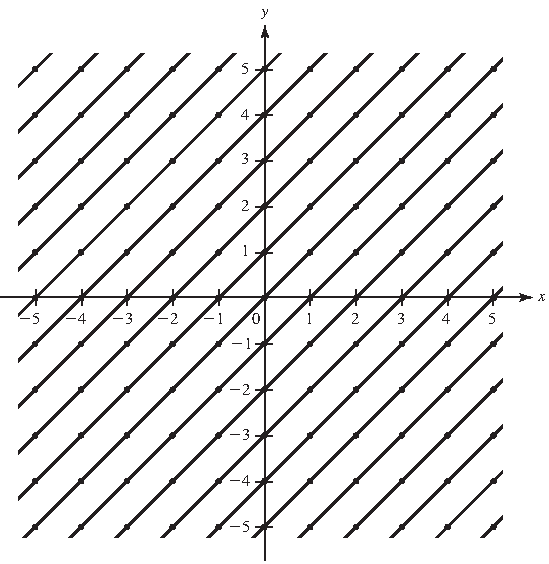
\includegraphics[width=0.752\linewidth,height=.8\textheight,keepaspectratio]{assets/p142_05.pdf}\end{center}
\begin{center}\small\textbf{13.13 Figure}\end{center}
\end{BookFloat}

\BookLabel{13.14 Example} We now compute \BookInline{(\mathbb{Z}\times \mathbb{Z})/\langle (2,\allowbreak 4)\rangle.} This is similar to Example 13.12, but there is a little twist to this one. In this example, we know that the factor group has an element with order 2, since \BookInline{(1,\allowbreak 2)\not \in \langle (2,\allowbreak 4)\rangle,\allowbreak } but \BookInline{(1,\allowbreak 2)+ (1,\allowbreak 2)\in \langle (2,\allowbreak 4)\rangle.} Furthermore\BookInline{,\allowbreak (\mathbb{Z}\times \mathbb{Z})/\langle (2,\allowbreak 4)\rangle } has an element \BookInline{(1,\allowbreak 0)+ \langle (2,\allowbreak 4)\rangle } with infinite order since \BookInline{(n,\allowbreak 0)\not \in \langle (2,\allowbreak 4)\rangle } for any \BookInline{n\in \mathbb{Z}^{+ }.} Figure 13.15 illustrates the situation. Along the line \BookInline{y= 2x} only every other lattice point is in \BookInline{\langle (2,\allowbreak 4)\rangle.} These points are filled dots in the figure. Each line with slope two contains 
% Source PDF page 143; original printed page 126
\BookSource{143}{126}
two cosets, one indicated with solid dots and one with hollow dots. Adding (1, 2) moves the solid dot cosets to the hollow dot cosets and the hollow dot cosets to the solid dot cosets while staying on the same line. Adding (0, 1) moves a coset from one line to the next. We may choose coset representatives

\end{BookBody}

\BookNarrativetrue

\begin{BookBody}

\begin{center}\begin{adjustbox}{max width=\linewidth}\BookInline{\displaystyle ...,\allowbreak (0,\allowbreak - 3),\allowbreak (0,\allowbreak - 2),\allowbreak (0,\allowbreak - 1),\allowbreak (0,\allowbreak 0),\allowbreak (0,\allowbreak 1),\allowbreak (0,\allowbreak 2),\allowbreak (0,\allowbreak 3),\allowbreak ...}\end{adjustbox}\end{center}

\noindent for the solid dot cosets and

\begin{center}\begin{adjustbox}{max width=\linewidth}\BookInline{\displaystyle ...,\allowbreak (1,\allowbreak - 3),\allowbreak (1,\allowbreak - 2),\allowbreak (1,\allowbreak - 1),\allowbreak (1,\allowbreak 0),\allowbreak (1,\allowbreak 1),\allowbreak (1,\allowbreak 2),\allowbreak (1,\allowbreak 3),\allowbreak ...}\end{adjustbox}\end{center}

\noindent for the hollow dot cosets. So it seems that we have two copies of the integers, one with a zero in the first coordinate and one with a one in the first coordinate. This leads us to guess that \BookInline{(\mathbb{Z}\times \mathbb{Z})/\langle (2,\allowbreak 4)\rangle } is isomorphic with \BookInline{\mathbb{Z}_{2}\times \mathbb{Z}.}

To verify that our guess is correct, we seek a homomorphism \BookInline{\phi:\mathbb{Z}\times \mathbb{Z}\to \mathbb{Z}_{2}\times \mathbb{Z}} that maps onto \BookInline{\mathbb{Z}_{2}\times \mathbb{Z}} and whose kernel is \BookInline{\langle (2,\allowbreak 4)\rangle.} We let \BookInline{\phi (a,\allowbreak b)= (r,\allowbreak 2a- b)} where \BookInline{r} is the remainder when \BookInline{a} is divided by 2. It is easy to check that \BookInline{\phi } is a homomorphism. Furthermore\BookInline{,\allowbreak \phi (0,\allowbreak - 1)= (0,\allowbreak 1)} and \BookInline{\phi (1,\allowbreak 2)= (1,\allowbreak 0),\allowbreak } which implies that \BookInline{\phi } maps onto \BookInline{\mathbb{Z}\times \mathbb{Z}_{2}.} It remains to compute Ker\BookInline{(\phi ).}

\begin{center}\begin{adjustbox}{max width=\linewidth}\BookInline{\displaystyle \;\text{Ker}\;(\phi )= \{(a,\allowbreak b)\mid b= 2a\;\text{and}\;a\;\text{is even}\;\}= \{(2n,\allowbreak 4n)\mid n\in \mathbb{Z}\}= \langle (2,\allowbreak 4)\rangle .}\end{adjustbox}\end{center}

\noindent Thus \BookInline{(\mathbb{Z}\times \mathbb{Z})/\langle (2,\allowbreak 4)\rangle } is isomorphic to \BookInline{\mathbb{Z}\times \mathbb{Z}_{2}} by the Fundamental Homomorphism Theorem. Furthermore, an isomorphism \BookInline{\mu:(\mathbb{Z}\times \mathbb{Z})/\langle (2,\allowbreak 4)\rangle \to \mathbb{Z}_{2}\times \mathbb{Z}} is defined by the formula \BookInline{\mu ((a,\allowbreak b)+ \langle (2,\allowbreak 4)\rangle )= (r,\allowbreak 2a- b)} where \BookInline{r} is the remainder when \BookInline{a} is divided by \BookInline{2.}\BookEnd{\blacktriangle}

\begin{BookFloat}{13_factor_group_computations_and_simple_groups-p143-8}
\begin{center}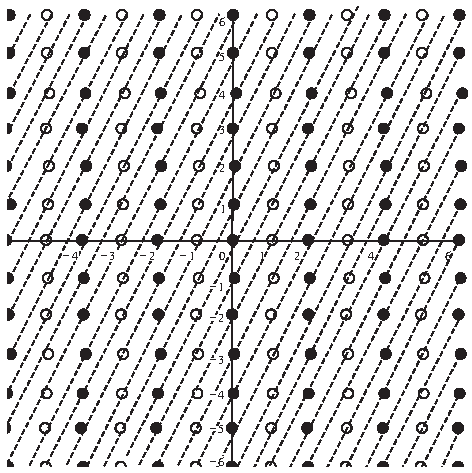
\includegraphics[width=0.647\linewidth,height=.8\textheight,keepaspectratio]{assets/p143_08.pdf}\end{center}
\begin{center}\small\textbf{13.15 Figure}\end{center}
\end{BookFloat}

\BookTextHeading{\textbf{Simple Groups}  }

\noindent As we mentioned in the preceding section, one feature of a factor group is that it gives crude information about the structure of the whole group. Of course, sometimes there may be no nontrivial proper normal subgroup. For example, Lagrange’s Theorem shows that a group of prime order can have no nontrivial proper subgroup of any sort.

\end{BookBody}

% Source PDF page 144; original printed page 127
\BookSource{144}{127}
\BookNarrativetrue

\begin{BookBody}

\BookLabel{13.16 Definition} A group is\textbf{ simple} if it is nontrivial and has no proper nontrivial normal subgroup\BookInline{.}\BookEnd{\blacksquare}

\BookLabel{13.17 Theorem} The alternating group \BookInline{A_{n}} is simple for \BookInline{n\geq 5.}

\BookLabel{\textit{Proof}} See Exercise 41. \BookEnd{\blacklozenge}

There are many simple groups other than those given above. For example\BookInline{,\allowbreak A_{5}} is of order 60 and \BookInline{A_{6}} is of order 360, and there is a simple group of nonprime order, namely 168, between these orders.

The complete determination and classification of all finite simple groups is one of the mathematical triumphs of the twentieth century. Hundreds of mathematicians worked on this task from 1950 to 1980. It can be shown that a finite group has a sort of factorization into simple groups, where the factors are unique up to order. The situation is similar to the factorization of positive integers into primes. The knowledge of all finite simple groups can be used to solve some problems of finite group theory and combinatorics.

We have seen in this text that a finite simple abelian group is isomorphic to \BookInline{\mathbb{Z}_{p}} for some prime \BookInline{p.} In 1963, Thompson and Feit [21] published their proof of a long-standing conjecture of Burnside, showing that every finite nonabelian simple group is of even order. Further great strides toward the complete classification were made by Aschbacher in the 1970s. Early in 1980, Griess announced that he had constructed a predicted “monster” simple group of order

808, 017, 424, 794, 512, 875, 886, 459, 904, 961, 710, 757, 005, 754, 368,

000, 000, 000.

\noindent Aschbacher added the final details of the classification in August 1980. The research papers contributing to the entire classification fill roughly 5000 journal pages.

We turn to the characterization of those normal subgroups \BookInline{N} of a group \BookInline{G} for which \BookInline{G/N} is a simple group. First we state an addendum to Theorem 8.5 on properties of a group homomorphism. The proof is left to Exercises 37 and 38.

\BookLabel{13.18 Theorem} Let \BookInline{\phi:G\to G^{\prime }} be a group homomorphism. If \BookInline{N} is a normal subgroup of \BookInline{G,\allowbreak } then \BookInline{\phi [N]} is a normal subgroup of \BookInline{\phi [G].} Also, if \BookInline{N^{\prime }} is a normal subgroup of \BookInline{\phi [G],\allowbreak } then \BookInline{\phi ^{- 1}[N^{\prime }]} is a normal subgroup of \BookInline{G.}\BookEnd{\blacklozenge}

Theorem 13.18 should be viewed as saying that a homomorphism \BookInline{\phi:G\to G^{\prime }} preserves normal subgroups between \BookInline{G} and \BookInline{\phi [G].} It is important to note that \BookInline{\phi [N]} may not be normal in \BookInline{G^{\prime },\allowbreak } even though \BookInline{N} is normal in \BookInline{G.} For example\BookInline{,\allowbreak \phi:\mathbb{Z}_{2}\to S_{3},\allowbreak } where \BookInline{\phi (0)= \iota } and \BookInline{\phi (1)= (1,\allowbreak 2)} is a homomorphism, and \BookInline{\mathbb{Z}_{2}} is a normal subgroup of itself, but \BookInline{\{\iota,\allowbreak (1,\allowbreak 2)\}} is not a normal subgroup of \BookInline{S_{3}.}

We can now characterize when \BookInline{G/N} is a simple group.

\BookLabel{13.19 Definition} A\textbf{ maximal normal subgroup of a group} \BookInline{G} is a normal subgroup \BookInline{M} not equal to \BookInline{G} such that there is no proper normal subgroup \BookInline{N} of \BookInline{G} properly containing \BookInline{M.}\BookEnd{\blacksquare}

\BookLabel{13.20 Theorem} \BookInline{M} is a maximal normal subgroup of \BookInline{G} if and only if \BookInline{G/M} is simple.

\BookLabel{\textit{Proof}} Let \BookInline{M} be a maximal normal subgroup of \BookInline{G.} Consider the canonical homomorphism \BookInline{\gamma:G\to G/M} given by Theorem 12.12. Now \BookInline{\gamma ^{- 1}} of any nontrivial proper normal subgroup of \BookInline{G/M} is a proper normal subgroup of \BookInline{G} properly containing \BookInline{M.} But \BookInline{M} is maximal, so this cannot happen. Thus \BookInline{G/M} is simple.

Conversely, Theorem 13.18 shows that if \BookInline{N} is a normal subgroup of \BookInline{G} properly containing \BookInline{M,\allowbreak } then \BookInline{\gamma [N]} is normal in \BookInline{G/M.} If also \BookInline{N\neq G,\allowbreak } then

\begin{center}\begin{adjustbox}{max width=\linewidth}\BookInline{\displaystyle \gamma [N]\neq  G/M\;\text{and}\;\gamma [N]\neq  \{M\}.}\end{adjustbox}\end{center}

\end{BookBody}

% Source PDF page 145; original printed page 128
\BookSource{145}{128}
\BookNarrativetrue

\begin{BookBody}

\noindent Thus, if \BookInline{G/M} is simple so that no such \BookInline{\gamma [N]} can exist, no such \BookInline{N} can exist, and \BookInline{M} is maximal\BookInline{.}\BookEnd{\blacklozenge}

\BookTextHeading{\textbf{The Center and Commutator Subgroups}  }

\noindent Every nonabelian group \BookInline{G} has two important normal subgroups, the\textit{ center} \BookInline{Z(G)} of \BookInline{G} and the\textit{ commutator subgroup} \BookInline{C} of \BookInline{G.(}The letter \BookInline{Z} comes from the German word \textit{zentrum,} meaning center.) The center \BookInline{Z(G)} is defined by

\begin{center}\begin{adjustbox}{max width=\linewidth}\BookInline{\displaystyle Z(G)= \{z\in G\mid zg= gz\;\text{for all}\;g\in G\}.}\end{adjustbox}\end{center}

\noindent Exercise 59 of Section 5 shows that \BookInline{Z(G)} is an abelian subgroup of \BookInline{G.} Since for each \BookInline{g\in } \BookInline{G} and \BookInline{z\in Z(G)} we have \BookInline{gzg^{- 1}= zgg^{- 1}= ze= z,\allowbreak } we see at once that \BookInline{Z(G)} is a normal subgroup of \BookInline{G.} If \BookInline{G} is abelian, then \BookInline{Z(G)= G;} in this case, the center is not useful.

\BookLabel{13.21 Example} The center of a group \BookInline{G} always contains the identity element \BookInline{e.} It may be that \BookInline{Z(G)= } \BookInline{\{e\},\allowbreak } in which case we say that\textbf{ the center of} \BookInline{G} \textbf{is trivial}. For example, examination of Table 4.15 for the group \BookInline{S_{3}} shows us that \BookInline{Z(S_{3})= \{\iota \},\allowbreak } so the center of \BookInline{S_{3}} is trivial. (This is a special case of Exercise 40, which shows that the center of every nonabelian group of order \BookInline{pq} for primes \BookInline{p} and \BookInline{q} is trivial.) Consequently, the center of \BookInline{S_{3}\times \mathbb{Z}_{5}} must be \BookInline{\{\iota \}\times \mathbb{Z}_{5},\allowbreak } which is isomorphic to \BookInline{\mathbb{Z}_{5}.}\BookEnd{\blacktriangle}

Turning to the commutator subgroup, recall that in forming a factor group of \BookInline{G} modulo a normal subgroup \BookInline{N,\allowbreak } we are essentially putting every element in \BookInline{G} that is in \BookInline{N} equal to \BookInline{e,\allowbreak } for \BookInline{N} forms our new identity in the factor group. This indicates another use for factor groups. Suppose, for example, that we are studying the structure of a nonabelian group \BookInline{G.} Since Theorem 9.12 gives complete information about the structure of all finitely generated abelian groups, it might be of interest to try to form an abelian group as much like \BookInline{G} as possible, an\textit{ abelianized version} of \BookInline{G,\allowbreak } by starting with \BookInline{G} and then requiring that \BookInline{ab= ba} for all \BookInline{a} and \BookInline{b} in our new group structure. To require that \BookInline{ab= ba} is to say that \BookInline{aba^{- 1}b^{- 1}= e} in our new group. An element \BookInline{aba^{- 1}b^{- 1}} in a group is a\textbf{ commutator of the group.} Thus we wish to attempt to form an abelianized version of \BookInline{G} by replacing every commutator of \BookInline{G} by \BookInline{e.} By the first observation of this paragraph, we should then attempt to form the factor group of \BookInline{G} modulo the smallest normal subgroup we can find that contains all commutators of \BookInline{G.}

\BookLabel{13.22 Theorem} Let \BookInline{G} be a group. The set of all commutators \BookInline{aba^{- 1}b^{- 1}} for \BookInline{a,\allowbreak b\in G} generates a subgroup \BookInline{C(}the\textbf{ commutator subgroup}) of \BookInline{G.} This subgroup \BookInline{C} is a normal subgroup of \BookInline{G.} Furthermore, if \BookInline{N} is a normal subgroup of \BookInline{G,\allowbreak } then \BookInline{G/N} is abelian if and only if \BookInline{C\leq N.}

\BookLabel{\textit{Proof}} The commutators certainly generate a subgroup \BookInline{C;} we must show that it is normal in \BookInline{G.} Note that the inverse \BookInline{(aba^{- 1}b^{- 1})^{- 1}} of a commutator is again a commutator, namely, \BookInline{bab^{- 1}a^{- 1}.} Also \BookInline{e= eee^{- 1}e^{- 1}} is a commutator. Theorem 7.7 then shows that \BookInline{C} consists precisely of all finite products of commutators. For \BookInline{x\in C,\allowbreak } we must show that \BookInline{g^{- 1}xg\in C} for all \BookInline{g\in G,\allowbreak } or that if \BookInline{x} is a product of commutators, so is \BookInline{g^{- 1}xg} for all \BookInline{g\in G.} By inserting \BookInline{e= gg^{- 1}} between each product of commutators occurring in \BookInline{x,\allowbreak } we see that it is sufficient to show for each commutator \BookInline{cdc^{- 1}d^{- 1}} that \BookInline{g^{- 1}(cdc^{- 1}d^{- 1})g} is in \BookInline{C.} But

\begin{center}\begin{adjustbox}{max width=\linewidth}\BookInline{\displaystyle \begin{aligned}g^{- 1}(cdc^{- 1}d^{- 1})g&= (g^{- 1}cdc^{- 1})(e)(d^{- 1}g) \\ &= (g^{- 1}cdc^{- 1})(gd^{- 1}dg^{- 1})(d^{- 1}g) \\ &= [(g^{- 1}c)d(g^{- 1}c)^{- 1}d^{- 1}][dg^{- 1}d^{- 1}g],\allowbreak \end{aligned}}\end{adjustbox}\end{center}

\noindent which is in \BookInline{C.} Thus \BookInline{C} is normal in \BookInline{G.}

\end{BookBody}

% Source PDF page 146; original printed page 129
\BookSource{146}{129}
\BookNarrativetrue

\begin{BookBody}

The rest of the theorem is obvious if we have acquired the proper feeling for factor groups. One doesn’t visualize in this way, but writing out that \BookInline{G/C} is abelian follows from

\begin{center}\begin{adjustbox}{max width=\linewidth}\BookInline{\displaystyle \begin{aligned}(aC)(bC)&= abC= ab(b^{- 1}a^{- 1}ba)C \\ &= (abb^{- 1}a^{- 1})baC= baC= (bC)(aC).\end{aligned}}\end{adjustbox}\end{center}

\noindent Furthermore, if \BookInline{N} is a normal subgroup of \BookInline{G} and \BookInline{G/N} is abelian, then \BookInline{(a^{- 1}N)(b^{- 1}N)= } \BookInline{(b^{- 1}N)(a^{- 1}N);} that is\BookInline{,\allowbreak aba^{- 1}b^{- 1}N= N,\allowbreak } so \BookInline{aba^{- 1}b^{- 1}\in N,\allowbreak } and \BookInline{C\leq N.} Finally, if \BookInline{C\leq } \BookInline{N,\allowbreak } then

\begin{center}\begin{adjustbox}{max width=\linewidth}\BookInline{\displaystyle \begin{aligned}(aN)(bN)&= abN= ab(b^{- 1}a^{- 1}ba)N \\ &= (abb^{- 1}a^{- 1})baN= baN= (bN)(aN).\end{aligned}}\end{adjustbox}\end{center} \BookEnd{\blacklozenge}

\BookLabel{13.23 Example} Using cycle notation in the symmetric group \BookInline{S_{3},\allowbreak } one commutator is

\begin{center}\begin{adjustbox}{max width=\linewidth}\BookInline{\displaystyle (1,\allowbreak 2,\allowbreak 3)(2,\allowbreak 3)(1,\allowbreak 2,\allowbreak 3)^{- 1}(2,\allowbreak 3)^{- 1}= (1,\allowbreak 2,\allowbreak 3)(2,\allowbreak 3)(1,\allowbreak 3,\allowbreak 2)(2,\allowbreak 3)= (1,\allowbreak 3,\allowbreak 2).}\end{adjustbox}\end{center}

\noindent So the commutator subgroup \BookInline{C} contains \BookInline{\langle (1,\allowbreak 3,\allowbreak 2)\rangle = A_{3},\allowbreak } the alternating group. Since \BookInline{S_{3}/A_{3}} is abelian (isomorphic with \BookInline{\mathbb{Z}_{2}),\allowbreak } Theorem 13.22 says that \BookInline{C\leq A_{3}.} Therefore\BookInline{,\allowbreak A_{3}} is the commutator subgroup\BookInline{.}\BookEnd{\blacktriangle}

\end{BookBody}

\BookNarrativefalse

\begin{BookBody}

\BookExerciseTitle{13} \BookEnd{\blacksquare}

\BookTextHeading{\textbf{Computations}}

\noindent In Exercises 1 through 14, classify the given group according to the fundamental theorem of finitely generated abelian groups.

\BookExercise{1.}{\BookInline{(\mathbb{Z}_{2}\times \mathbb{Z}_{4})/\langle (0,\allowbreak 1)\rangle }}

\BookExercise{2.}{\BookInline{(\mathbb{Z}_{2}\times \mathbb{Z}_{4})/\langle (0,\allowbreak 2)\rangle }}

\BookExercise{3.}{\BookInline{(\mathbb{Z}_{2}\times \mathbb{Z}_{4})/\langle (1,\allowbreak 2)\rangle }}

\BookExercise{4.}{\BookInline{(\mathbb{Z}_{4}\times \mathbb{Z}_{8})/\langle (1,\allowbreak 2)\rangle }}

\BookExercise{5.}{\BookInline{(\mathbb{Z}_{4}\times \mathbb{Z}_{4}\times \mathbb{Z}_{8})/\langle (1,\allowbreak 2,\allowbreak 4)\rangle }}

\BookExercise{6.}{\BookInline{(\mathbb{Z}\times \mathbb{Z})/\langle (0,\allowbreak 1)\rangle }}

\BookExercise{7.}{\BookInline{(\mathbb{Z}\times \mathbb{Z})/\langle (0,\allowbreak 2)\rangle }}

\BookExercise{8.}{\BookInline{(\mathbb{Z}\times \mathbb{Z}\times \mathbb{Z})/\langle (1,\allowbreak 1,\allowbreak 1)\rangle }}

\BookExercise{9.}{\BookInline{(\mathbb{Z}\times \mathbb{Z}\times \mathbb{Z}_{4})/\langle (3,\allowbreak 0,\allowbreak 0)\rangle }}

\BookExercise{10.}{\BookInline{(\mathbb{Z}\times \mathbb{Z}\times \mathbb{Z}_{8})/\langle (0,\allowbreak 4,\allowbreak 0)\rangle }}

\BookExercise{11.}{\BookInline{(\mathbb{Z}\times \mathbb{Z})/\langle (2,\allowbreak 2)\rangle }}

\BookExercise{12.}{\BookInline{(\mathbb{Z}\times \mathbb{Z}\times \mathbb{Z})/\langle (3,\allowbreak 3,\allowbreak 3)\rangle }}

\BookExercise{13.}{\BookInline{(\mathbb{Z}\times \mathbb{Z})/\langle (2,\allowbreak 6)\rangle }}

\BookExercise{14.}{\BookInline{(\mathbb{Z}\times \mathbb{Z}\times \mathbb{Z}_{2})/\langle (1,\allowbreak 1,\allowbreak 1)\rangle }}

\BookExercise{15.}{Find both the center and the commutator subgroup of \BookInline{D_{4}.}}

\BookExercise{16.}{Find both the center and the commutator subgroup of \BookInline{\mathbb{Z}_{3}\times S_{3}.}}

\BookExercise{17.}{Find both the center and the commutator subgroup of \BookInline{S_{3}\times D_{4}.}}

\BookExercise{18.}{Describe all subgroups of order \BookInline{\leq 4} of \BookInline{\mathbb{Z}_{4}\times \mathbb{Z}_{4},\allowbreak } and in each case classify the factor group of \BookInline{\mathbb{Z}_{4}\times \mathbb{Z}_{4}} modulo the subgroup by Theorem 9.12. That is, describe the subgroup and say that the factor group of \BookInline{\mathbb{Z}_{4}\times \mathbb{Z}_{4}} modulo the subgroup is isomorphic to \BookInline{\mathbb{Z}_{2}\times \mathbb{Z}_{4},\allowbreak } or whatever the case may be. [\textit{Hint}\BookInline{:\mathbb{Z}_{4}\times \mathbb{Z}_{4}} has six different cyclic subgroups of order 4. Describe them by giving a generator, such as the subgroup \BookInline{\langle (1,\allowbreak 0)\rangle.} There is one subgroup of order 4 that is isomorphic to the Klein 4-group. There are three subgroups of order 2.]}

\BookTextHeading{\textbf{Concepts}}

\noindent In Exercises 19 and 20, correct the definition of the italicized term without reference to the text, if correction is needed, so that it is in a form acceptable for publication.

\BookExercise{19.}{The\textit{ center} of a group \BookInline{G} contains all elements of \BookInline{G} that commute with every element of \BookInline{G.}}

\BookExercise{20.}{The\textit{ commutator subgroup} of a group \BookInline{G} is \BookInline{\{a^{- 1}b^{- 1}ab\mid a,\allowbreak b\in G\}.}}

\end{BookBody}

% Source PDF page 147; original printed page 130
\BookSource{147}{130}
\BookNarrativefalse

\begin{BookBody}

\BookExercise{21.}{Determine whether each of following is true or false.}

\BookExercise{a.}{Every factor group of a cyclic group is cyclic.}

\BookExercise{b.}{A factor group of a noncyclic group is again noncyclic.}

\BookExercise{c.}{\textbf{c}\BookInline{.\mathbb{R}/\mathbb{Z}} under addition has no element of order 3.}

\BookExercise{d.}{\textbf{d}\BookInline{.\mathbb{R}/\mathbb{Q}} under addition has no element of order 2.}

\BookExercise{e.}{\textbf{e}\BookInline{.\mathbb{R}/\mathbb{Z}} under addition has an infinite number of elements of order 4.}

\BookExercise{f.}{If the commutator subgroup \BookInline{C} of a group \BookInline{G} is \BookInline{\{e\},\allowbreak } then \BookInline{G} is abelian.}

\BookExercise{g.}{If \BookInline{G/H} is abelian, then the commutator subgroup \BookInline{C} of \BookInline{G} contains \BookInline{H.}}

\BookExercise{h.}{The commutator subgroup of a simple group \BookInline{G} must be \BookInline{G} itself.}

\BookExercise{i.}{The commutator subgroup of a nonabelian simple group \BookInline{G} must be \BookInline{G} itself.}

\BookExercise{j.}{All nontrivial finite simple groups have prime order.}

\noindent In Exercises 22 through 25, let \BookInline{F} be the additive group of all functions mapping \BookInline{\mathbb{R}} into \BookInline{\mathbb{R},\allowbreak } and let \BookInline{F^{\ast }} be the multiplicative group of all elements of \BookInline{F} that do not assume the value 0 at any point of \BookInline{\mathbb{R}.}

\BookExercise{22.}{Let \BookInline{K} be the subgroup of \BookInline{F} consisting of the constant functions. Find a subgroup of \BookInline{F} to which \BookInline{F/K} is isomorphic.}

\BookExercise{23.}{Let \BookInline{K^{\ast }} be the subgroup of \BookInline{F^{\ast }} consisting of the nonzero constant functions. Find a subgroup of \BookInline{F^{\ast }} to which \BookInline{F^{\ast }/K^{\ast }} is isomorphic.}

\BookExercise{24.}{Let \BookInline{K} be the subgroup of continuous functions in \BookInline{F.} Can you find an element of \BookInline{F/K} having order 2? Why or why not?}

\BookExercise{25.}{Let \BookInline{K^{\ast }} be the subgroup of \BookInline{F^{\ast }} consisting of the continuous functions in \BookInline{F^{\ast }.} Can you find an element of \BookInline{F^{\ast }/K^{\ast }} having order 2? Why or why not?}

\noindent In Exercises 26 through 28, let \BookInline{U} be the multiplicative group \BookInline{\{ z \in \mathbb { C } \big | | z | = 1 \}}.

\BookExercise{26.}{Let \BookInline{z_{0}\in U.} Show that \BookInline{z_{0}U= \{z_{0}z\mid z\in U\}} is a subgroup of \BookInline{U,\allowbreak } and compute \BookInline{U/z_{0}U.}}

\BookExercise{27.}{To what group we have mentioned in the text is \BookInline{U/\langle - 1\rangle } isomorphic?}

\BookExercise{28.}{Let \BookInline{\zeta _{n}= } cos\BookInline{(2\pi /n)+ i} sin\BookInline{(2\pi /n)} where \BookInline{n\in \mathbb{Z}^{+ }.} To what group we have mentioned is \BookInline{U/\langle \zeta _{n}\rangle } isomorphic?}

\BookExercise{29.}{To what group mentioned in the text is the additive group \BookInline{\mathbb{R}/\mathbb{Z}} isomorphic?}

\BookExercise{30.}{Give an example of a group \BookInline{G} having no elements of finite order greater than 1 and a normal subgroup \BookInline{H\unlhd G,\allowbreak } \BookInline{H\neq G,\allowbreak } so that in \BookInline{G/H} every element has finite order.}

\BookExercise{31.}{Let \BookInline{H} and \BookInline{K} be normal subgroups of a group \BookInline{G.} Give an example showing that we may have \BookInline{H\simeq K} while \BookInline{G/H} is not isomorphic to \BookInline{G/K.}}

\BookExercise{32.}{Describe the center of every simple}

\BookExercise{a.}{abelian group}

\BookExercise{b.}{nonabelian group.}

\BookExercise{33.}{Describe the commutator subgroup of every simple}

\BookExercise{a.}{abelian group}

\BookExercise{b.}{nonabelian group.}

\BookLabel{\textit{Proof}} \textbf{ Synopsis}

\BookExercise{34.}{Give a one-sentence synopsis of the proof of Theorem 13.9.}

\BookExercise{35.}{Give at most a two-sentence synopsis of the proof of Theorem 13.20.}

\BookTextHeading{\textbf{Theory}}

\BookExercise{36.}{Show that if a finite group \BookInline{G} contains a nontrivial subgroup of index 2 in \BookInline{G,\allowbreak } then \BookInline{G} is not simple.}

\BookExercise{37.}{Let \BookInline{\phi:G\to G^{\prime }} be a group homomorphism, and let \BookInline{N} be a normal subgroup of \BookInline{G.} Show that \BookInline{\phi [N]} is a normal subgroup of \BookInline{\phi [G].}}

\end{BookBody}

% Source PDF page 148; original printed page 131
\BookSource{148}{131}
\BookNarrativefalse

\begin{BookBody}

\BookExercise{38.}{Let \BookInline{\phi:G\to G^{\prime }} be a group homomorphism, and let \BookInline{N^{\prime }} be a normal subgroup of \BookInline{G^{\prime }.} Show that \BookInline{\phi ^{- 1}[N^{\prime }]} is a normal subgroup of \BookInline{G.}}

\BookExercise{39.}{Show that if \BookInline{G} is nonabelian, then the factor group \BookInline{G/Z(G)} is not cyclic. [\textit{Hint:} Show the equivalent contrapositive, namely, that if \BookInline{G/Z(G)} is cyclic then \BookInline{G} is abelian (and hence \BookInline{Z(G)= G).]}}

\BookExercise{40.}{Using Exercise 39, show that a nonabelian group \BookInline{G} of order \BookInline{pq} where \BookInline{p} and \BookInline{q} are primes has a trivial center.}

\BookExercise{41.}{Prove that \BookInline{A_{n}} is simple for \BookInline{n\geq 5,\allowbreak } following the steps and hints given.}

\BookExercise{a.}{Show \BookInline{A_{n}} contains every 3-cycle if \BookInline{n\geq 3.}}

\BookExercise{b.}{Show \BookInline{A_{n}} is generated by the 3-cycles for \BookInline{n\geq 3.[}\textit{Hint:} Note that \BookInline{(a,\allowbreak b)(c,\allowbreak d)= (a,\allowbreak c,\allowbreak b)(a,\allowbreak c,\allowbreak d)} and \BookInline{(a,\allowbreak c)(a,\allowbreak b)= (a,\allowbreak b,\allowbreak c).]}}

\BookExercise{c.}{Let \BookInline{r} and \BookInline{s} be fixed elements of \BookInline{\{1,\allowbreak 2,\allowbreak \cdots,\allowbreak n\}} for \BookInline{n\geq 3.} Show that \BookInline{A_{n}} is generated by the \BookInline{n} “special” 3cycles of the form \BookInline{(r,\allowbreak s,\allowbreak i)} for \BookInline{1\leq i\leq n[}\textit{Hint:} Show every 3-cycle is the product of “special” 3-cycles by computing}

\begin{center}\begin{adjustbox}{max width=\linewidth}\BookInline{\displaystyle (r,\allowbreak s,\allowbreak i)^{2},\allowbreak (r,\allowbreak s,\allowbreak j)(r,\allowbreak s,\allowbreak i)^{2},\allowbreak (r,\allowbreak s,\allowbreak j)^{2}(r,\allowbreak s,\allowbreak i),\allowbreak }\end{adjustbox}\end{center}

and

\begin{center}\begin{adjustbox}{max width=\linewidth}\BookInline{\displaystyle (r,\allowbreak s,\allowbreak i)^{2}(r,\allowbreak s,\allowbreak k)(r,\allowbreak s,\allowbreak j)^{2}(r,\allowbreak s,\allowbreak i).}\end{adjustbox}\end{center}

Observe that these products give all possible types of 3-cycles.]

\BookExercise{d.}{Let \BookInline{N} be a normal subgroup of \BookInline{A_{n}} for \BookInline{n\geq 3.} Show that if \BookInline{N} contains a 3-cycle, then \BookInline{N= A_{n}.[}\textit{Hint:} Show that \BookInline{(r,\allowbreak s,\allowbreak i)\in N} implies that \BookInline{(r,\allowbreak s,\allowbreak j)\in N} for \BookInline{j= 1,\allowbreak 2,\allowbreak \cdots,\allowbreak n} by computing}

\begin{center}\begin{adjustbox}{max width=\linewidth}\BookInline{\displaystyle ((r,\allowbreak s)(i,\allowbreak j))(r,\allowbreak s,\allowbreak i)^{2}((r,\allowbreak s)(i,\allowbreak j))^{- 1}.]}\end{adjustbox}\end{center}

\BookExercise{e.}{Let \BookInline{N} be a nontrivial normal subgroup of \BookInline{A_{n}} for \BookInline{n\geq 5.} Show that one of the following cases must hold, and conclude in each case that \BookInline{N= A_{n}.}}

\textbf{Case I} \BookInline{N} contains a 3-cycle.

\textbf{Case II} \BookInline{N} contains a product of disjoint cycles, at least one of which has length greater than 3. [\textit{Hint:} Suppose \BookInline{N} contains the disjoint product \BookInline{\sigma = \mu (a_{1},\allowbreak a_{2},\allowbreak \cdots,\allowbreak a_{r}).} Show \BookInline{\sigma ^{- 1}(a_{1},\allowbreak a_{2},\allowbreak a_{3})\sigma (a_{1},\allowbreak a_{2},\allowbreak a_{3})^{- 1}} is in \BookInline{N,\allowbreak } and compute it.]

\textbf{Case III} \BookInline{N} contains a disjoint product of the form \BookInline{\sigma = \mu (a_{4},\allowbreak a_{5},\allowbreak a_{6})(a_{1},\allowbreak a_{2},\allowbreak a_{3}).[}\textit{Hint:} Show \BookInline{\sigma ^{- 1}(a_{1},\allowbreak a_{2},\allowbreak a_{4})} \BookInline{\sigma (a_{1},\allowbreak a_{2},\allowbreak a_{4})^{- 1}} is in \BookInline{N,\allowbreak } and compute it.]

\textbf{Case IV} \BookInline{N} contains a disjoint product of the form \BookInline{\sigma = \mu (a_{1},\allowbreak a_{2},\allowbreak a_{3})} where \BookInline{\mu } is a product of disjoint 2cycles. [\textit{Hint:} Show \BookInline{\sigma ^{2}\in N} and compute it.]

\textbf{Case V} \BookInline{N} contains a disjoint product \BookInline{\sigma } of the form \BookInline{\sigma = \mu (a_{3},\allowbreak a_{4})(a_{1},\allowbreak a_{2}),\allowbreak } where \BookInline{\mu } is a product of an even number of disjoint 2-cycles. [\textit{Hint:} Show that \BookInline{\sigma ^{- 1}(a_{1},\allowbreak a_{2},\allowbreak a_{3})\sigma (a_{1},\allowbreak a_{2},\allowbreak a_{3})^{- 1}} is in \BookInline{N,\allowbreak } and compute it to deduce that \BookInline{\alpha = (a_{2},\allowbreak a_{4})(a_{1},\allowbreak a_{3})} is in \BookInline{N.} Using \BookInline{n\geq 5} for the first time, find \BookInline{i\neq a_{1},\allowbreak a_{2},\allowbreak a_{3},\allowbreak a_{4}} in \BookInline{\{1,\allowbreak 2,\allowbreak \cdots,\allowbreak n\}.} Let \BookInline{\beta = (a_{1},\allowbreak a_{3},\allowbreak i).} Show that \BookInline{\beta ^{- 1}\alpha \beta \alpha \in N,\allowbreak } and compute it.]

\BookExercise{42.}{Let \BookInline{N} be a normal subgroup of \BookInline{G} and let \BookInline{H} be any subgroup of \BookInline{G.} Let \BookInline{HN= \{hn\mid h\in H,\allowbreak n\in N\}.} Show that \BookInline{HN} is a subgroup of \BookInline{G,\allowbreak } and is the smallest subgroup containing both \BookInline{N} and \BookInline{H.}}

\BookExercise{43.}{With reference to the preceding exercise, let \BookInline{M} also be a normal subgroup of \BookInline{G.} Show that \BookInline{NM} is again a normal subgroup of \BookInline{G.}}

\BookExercise{44.}{Show that if \BookInline{H} and \BookInline{K} are normal subgroups of a group \BookInline{G} such that \BookInline{H\cap K= \{e\},\allowbreak } then \BookInline{hk= kh} for all \BookInline{h\in H} and \BookInline{k\in K.[}\textit{Hint:} Consider the commutator \BookInline{hkh^{- 1}k^{- 1}= (hkh^{- 1})k^{- 1}= h(kh^{- 1}k^{- 1}).]}}

\BookExercise{45.}{With reference to the three preceding exercises, let \BookInline{H} and \BookInline{K} be normal subgroups of a group \BookInline{G} such that \BookInline{HK= G} and \BookInline{H\cap K= \{e\}.} Prove that \BookInline{G} is isomorphic with \BookInline{H\times G.}}

\end{BookBody}
\ifdefined\BookMaster\let\BookFinish\relax\else\def\BookFinish{\end{document}}\fi\BookFinish

\clearpage
% !TeX program = xelatex
\ifdefined\BookMaster\else
\documentclass[11pt,oneside]{article}
% !TeX program = xelatex
\usepackage[b5paper,left=22mm,right=22mm,top=20mm,bottom=22mm,footskip=11mm]{geometry}
\usepackage{fontspec}
\setmainfont{TeX Gyre Termes}
\setsansfont{TeX Gyre Heros}
\usepackage{amsmath,amssymb,mathtools,amsthm}
\renewcommand{\cdots}{\mathinner{\cdotp\cdotp\cdotp}}
\usepackage{graphicx,adjustbox,array,booktabs,longtable,multirow,enumitem,changepage,needspace}
\usepackage[table]{xcolor}
\usepackage{fancyhdr}
\raggedbottom
\interfootnotelinepenalty=10000
\newcommand{\BookFootnote}[2]{\begingroup\renewcommand{\thefootnote}{\fnsymbol{footnote}}\footnote[#1]{#2}\endgroup}
\newcommand{\BookFootnoteMark}[1]{\begingroup\renewcommand{\thefootnote}{\fnsymbol{footnote}}\footnotemark[#1]\endgroup}
\newcommand{\BookFootnoteText}[2]{\begingroup\renewcommand{\thefootnote}{\fnsymbol{footnote}}\footnotetext[#1]{#2}\endgroup}
\newenvironment{BookFloat}[1]{\par\addvspace{.6\baselineskip}\noindent\def\BookFloatID{#1}\begin{minipage}{\linewidth}\phantomsection\label{bookfloat:#1:start}}{\phantomsection\label{bookfloat:\BookFloatID:end}\end{minipage}\par\addvspace{.6\baselineskip}}

\usepackage[unicode,hidelinks]{hyperref}
\pagestyle{fancy}
\fancyhf{}
\newcommand{\BookFooter}{}
\fancyfoot[L]{\parbox[b]{\dimexpr\textwidth-15mm}{\footnotesize\BookFooter}}
\fancyfoot[R]{\footnotesize\thepage}
\renewcommand{\headrulewidth}{0pt}
\renewcommand{\footrulewidth}{0pt}
\setlength{\parindent}{0pt}
\setlength{\parskip}{0.2em}
\setlength{\emergencystretch}{3em}
\setlist{nosep,leftmargin=1.7em,labelsep=.65em}
\newif\ifBookNarrative
\BookNarrativetrue
\newenvironment{BookBody}{\setlength{\parindent}{0pt}}{}
\newcommand{\BookStatement}[1]{\par\addvspace{.6\baselineskip}\noindent #1\enspace\ignorespaces}
\newcommand{\BookLabel}[1]{\par\addvspace{.6\baselineskip}\needspace{3\baselineskip}\noindent\textbf{#1}\quad\ignorespaces}
\newcommand{\BookHeading}[1]{\par\addvspace{\baselineskip}\needspace{4\baselineskip}\noindent{\large\bfseries #1}\par\medskip}
\newcommand{\BookSubheading}[1]{\par\addvspace{.7\baselineskip}\needspace{3\baselineskip}\noindent{\bfseries #1}\par\smallskip}
\newcommand{\BookTextHeading}[1]{\par\addvspace{.7\baselineskip}\needspace{3\baselineskip}\noindent #1\par\smallskip}
\newcommand{\BookSectionTitle}[2]{\par\addvspace{1.2\baselineskip}\needspace{5\baselineskip}\noindent\colorbox{gray!25}{\sffamily\bfseries\small SECTION #1}\quad{\large\bfseries #2}\par\medskip}
\newcommand{\BookExerciseTitle}[1]{\par\addvspace{\baselineskip}\needspace{4\baselineskip}\noindent{\color{gray}\rule{1.5mm}{1.5mm}}\enspace{\large\bfseries Exercises #1}\par\medskip}
\newcommand{\BookBullet}[1]{\begin{list}{\textbullet}{\setlength{\leftmargin}{1.7em}\setlength{\labelwidth}{1em}\setlength{\labelsep}{.7em}\setlength{\topsep}{0pt}\setlength{\parsep}{0pt}\setlength{\itemsep}{0pt}}\item #1\end{list}}
\newcommand{\BookExercise}[2]{\begin{list}{\textbf{#1}}{\setlength{\leftmargin}{2.2em}\setlength{\labelwidth}{1.5em}\setlength{\labelsep}{.7em}\setlength{\topsep}{.15em}\setlength{\parsep}{0pt}\setlength{\itemsep}{0pt}}\item #2\end{list}}
\newcommand{\BookEnd}[1]{\unskip\nobreak\hfill\ensuremath{#1}}
\newcommand{\BookSource}[2]{\phantomsection\label{sourcepage:#1}} % Source-page anchors, retained through reflow.
\usepackage{multicol}
\usepackage{tikz}
\newcommand{\BookPartEntry}[2]{\par\noindent\makebox[17mm][l]{\bfseries Section #1}#2\par}
\newcommand{\BookPartTitle}[3]{\par\bigskip\noindent\begin{tikzpicture}\node[anchor=north west,inner sep=0pt,outer sep=0pt] (bookpart) at (0,0) {\begin{minipage}{\dimexpr\linewidth-.5pt}\hspace*{26mm}\begin{minipage}[t]{\dimexpr\linewidth-26mm}\begin{adjustbox}{max width=\linewidth}{\fontsize{20}{24}\selectfont\bfseries #2}\end{adjustbox}\par\vspace{6mm}\hrule\vspace{6mm}{\sffamily\footnotesize\setlength{\parskip}{.3em}#3}\vspace{3mm}\end{minipage}\end{minipage}};\path[shade,top color=gray!60,bottom color=white] (0,0) rectangle ([xshift=24mm]bookpart.south west);\node[anchor=north,font=\sffamily\bfseries\small] at (12mm,-2mm) {PART};\node[anchor=north,font=\sffamily\bfseries\Huge] at (12mm,-7mm) {#1};\end{tikzpicture}\par\bigskip}
\newsavebox{\BookMathBox}
\makeatletter
\newcommand{\BookInline}[1]{\leavevmode\hskip0pt\relax\begingroup\in@{\begin}{#1}\ifin@\sbox{\BookMathBox}{\(#1\)}\ifdim\wd\BookMathBox>\dimexpr\linewidth-1em\relax\resizebox{\dimexpr\linewidth-1em\relax}{!}{\usebox{\BookMathBox}}\else\(#1\)\fi\else\in@{\left}{#1}\ifin@\sbox{\BookMathBox}{\(#1\)}\ifdim\wd\BookMathBox>\dimexpr\linewidth-1em\relax\resizebox{\dimexpr\linewidth-1em\relax}{!}{\usebox{\BookMathBox}}\else\(#1\)\fi\else\(#1\)\fi\fi\endgroup\hskip0pt\relax}
\makeatother
\DeclareMathOperator{\Aut}{Aut}
\DeclareMathOperator{\End}{End}
\DeclareMathOperator{\Hom}{Hom}
\DeclareMathOperator{\GF}{GF}
\DeclareMathOperator{\irr}{irr}
\DeclareMathOperator{\lt}{lt}
\DeclareMathOperator{\lp}{lp}
\providecommand{\textcircled}[1]{\textnormal{(#1)}}

\begin{document}
\fi
\renewcommand{\BookFooter}{Section 14 Group Action on a Set}
\pdfbookmark[0]{Section 14 Group Action on a Set}{14_group_action_on_a_set}
\ifdefined\BookMaster\else\setcounter{page}{132}\fi
% Source PDF page 149; original printed page 132
\BookSource{149}{132}
\BookNarrativetrue

\begin{BookBody}

\BookSectionTitle{14}{Group Action on a Set\label{bookfootnote:149:2:ref}\BookFootnote{2}{\label{bookfootnote:149:2:text}This section is a prerequisite only for Sections 15 and 17.}}

\noindent We have seen examples of how groups may\textit{ act on things}, like the group of symmetries of a triangle or of a square, the group of rotations of a cube, the general linear group acting on \BookInline{\mathbb{R}^{n},\allowbreak } and so on. In this section we give the general notion of group action and apply it to learn more about finite groups. The next section will give applications to counting.

\BookTextHeading{\textbf{The Notion of a Group Action}  }

\noindent Definition 1.1 defines a binary operation \BookInline{\ast } on a set \BookInline{S} to be a function mapping \BookInline{S\times S} into \BookInline{S.} The function \BookInline{\ast } gives us a rule for “multiplying” an element \BookInline{s_{1}} in \BookInline{S} and an element \BookInline{s_{2}} in \BookInline{S} to yield an element \BookInline{s_{1}\ast s_{2}} in \BookInline{S.}

More generally, for any sets \BookInline{A,\allowbreak B,\allowbreak } and \BookInline{C,\allowbreak } we can view a map \BookInline{\ast:A\times B\to C} as defining a “multiplication,” where any element \BookInline{a} of \BookInline{A} times any element \BookInline{b} of \BookInline{B} has as value some element \BookInline{c} of \BookInline{C.} Of course, we write \BookInline{a\ast b= c,\allowbreak } or simply \BookInline{ab= c.} In this section, we will be concerned with the case where \BookInline{X} is a set\BookInline{,\allowbreak G} is a group, and we have a map \BookInline{\ast:G\times X\to X.} We shall write \BookInline{\ast (g,\allowbreak x)} as \BookInline{g\ast x} or \BookInline{gx.}

\BookLabel{14.1 Example} Let \BookInline{G= } GL\BookInline{(n,\allowbreak \mathbb{R})} and \BookInline{X} the set of all column vectors in \BookInline{\mathbb{R}^{n}.} Then for any matrix \BookInline{A\in G} and vector \BookInline{v\in X,\allowbreak Av} is a vector in \BookInline{X.} So multiplying is an operation \BookInline{\ast:G\times X\to X.} From linear algebra, we know that if \BookInline{B} is also a matrix in \BookInline{G,\allowbreak } then \BookInline{(AB)v= A(Bv).} Furthermore, for the identity matrix \BookInline{I,\allowbreak } \textit{Iv} \BookInline{= v.}\BookEnd{\blacktriangle}

\BookLabel{14.2 Example} Let \BookInline{G} be the dihedral group \BookInline{D_{n}.} Then elements of \BookInline{D_{n}} permute the set \BookInline{\mathbb{Z}_{n}= } \BookInline{\{0,\allowbreak 1,\allowbreak 2,\allowbreak 3,\allowbreak...,\allowbreak n- 1\}.} For example\BookInline{,\allowbreak \rho (k)= k+ _{n}1.} Thus we have an operation \BookInline{\ast:} \BookInline{D_{n}\times \mathbb{Z}_{n}\to \mathbb{Z}_{n}.} Furthermore, if \BookInline{\alpha,\allowbreak \gamma \in D_{n}} and \BookInline{k\in \mathbb{Z}_{n},\allowbreak } then \BookInline{(\alpha \gamma )(k)= \alpha (\gamma (k))} and \BookInline{\iota (k)= k.}\BookEnd{\blacktriangle}

\noindent The two previous examples share the same properties, which we formalize in Definition 14.3.

\BookLabel{14.3 Definition} Let \BookInline{X} be a set and \BookInline{G} a group. An\textbf{ action of} \BookInline{G} \textbf{on} \BookInline{X} is a map \BookInline{\ast:G\times X\to X} such that

\BookExercise{1.}{\textit{ex} \BookInline{= x} for all \BookInline{x\in X,\allowbreak }}

\BookExercise{2.}{\BookInline{(g_{1}g_{2})(x)= g_{1}(g_{2}x)} for all \BookInline{x\in X} and all \BookInline{g_{1},\allowbreak g_{2}\in G.}}

Under these conditions\BookInline{,\allowbreak X} is a \BookInline{G-}\textbf{set.} \BookEnd{\blacksquare}

\BookLabel{14.4 Example} Let \BookInline{X} be any set, and let \BookInline{H} be a subgroup of the group \BookInline{S_{X}} of all permutations of \BookInline{X.} Then \BookInline{X} is an \BookInline{H-}set, where the action of \BookInline{\sigma \in H} on \BookInline{X} is its action as an element of \BookInline{S_{X},\allowbreak } so that \BookInline{\sigma x= \sigma (x)} for all \BookInline{x\in X.} Condition 2 is a consequence of the definition of permutation multiplication as function composition, and Condition 1 is immediate from the definition of the identity permutation as the identity function. Note that, in particular, \BookInline{\{1,\allowbreak 2,\allowbreak 3,\allowbreak \cdots,\allowbreak n\}} is an \BookInline{S_{n}-}set\BookInline{.}\BookEnd{\blacktriangle}

Our next theorem will show that for every \BookInline{G-}set \BookInline{X} and each \BookInline{g\in G,\allowbreak } the map \BookInline{\sigma _{g}:X\to X} defined by \BookInline{\sigma _{g}(x)= gx} is a permutation of \BookInline{X,\allowbreak } and that there is a homomorphism \BookInline{\phi:G\to S_{X}} such that the action of \BookInline{G} on \BookInline{X} is essentially the Example 14.4 action of the image subgroup \BookInline{H= \phi [G]} of \BookInline{S_{X}} on \BookInline{X.} So actions of subgroups of \BookInline{S_{X}} on \BookInline{X} describe all possible group actions on \BookInline{X.} When studying the set \BookInline{X,\allowbreak } actions using subgroups of \BookInline{S_{X}} suffice. However, sometimes a set \BookInline{X} is used to study \BookInline{G} via a group action of \BookInline{G} on \BookInline{X.} Thus we need the more general concept given by Definition 14.3.

\end{BookBody}

% Source PDF page 150; original printed page 133
\BookSource{150}{133}
\BookNarrativetrue

\begin{BookBody}

\BookLabel{14.5 Theorem} Let \BookInline{X} be a \BookInline{G-}set. For each \BookInline{g\in G,\allowbreak } the function \BookInline{\sigma _{g}:X\to X} defined by \BookInline{\sigma _{g}(x)= gx} for \BookInline{x\in X} is a permutation of \BookInline{X.} Also, the map \BookInline{\phi:G\to S_{X}} defined by \BookInline{\phi (g)= \sigma _{g}} is a homomorphism with the property that \BookInline{\phi (g)(x)= gx.}

\BookLabel{\textit{Proof}} To show that \BookInline{\sigma _{g}} is a permutation of \BookInline{X,\allowbreak } we must show that \BookInline{\sigma _{g}} is a one-to-one map of \BookInline{X} onto itself. Suppose that \BookInline{\sigma _{g}(x_{1})= \sigma _{g}(x_{2})} for \BookInline{x_{1},\allowbreak x_{2}\in X.} Then \BookInline{gx_{1}= gx_{2}.} Consequently\BookInline{,\allowbreak g^{- 1}(gx_{1})= g^{- 1}(gx_{2}).} Using Condition 2 in Definition 14.3, we see that \BookInline{(g^{- 1}g)x_{1}= (g^{- 1}g)x_{2},\allowbreak } so \BookInline{ex_{1}= ex_{2}.} Condition 1 of the definition then yields \BookInline{x_{1}= x_{2},\allowbreak } so \BookInline{\sigma _{g}} is one-to-one. The two conditions of the definition show that for \BookInline{x\in X,\allowbreak } we have \BookInline{\sigma _{g}(g^{- 1}x)= g(g^{- 1})x= (gg^{- 1})x= } \textit{ex} \BookInline{= x,\allowbreak } so \BookInline{\sigma _{g}} maps \BookInline{X} onto \BookInline{X.} Thus \BookInline{\sigma _{g}} is indeed a permutation.

To show that \BookInline{\phi:G\to S_{X}} defined by \BookInline{\phi (g)= \sigma _{g}} is a homomorphism, we must show that \BookInline{\phi (g_{1}g_{2})= \phi (g_{1})\phi (g_{2})} for all \BookInline{g_{1},\allowbreak g_{2}\in G.} We show the equality of these two permutations in \BookInline{S_{X}} by showing they both carry an \BookInline{x\in X} into the same element. Using the two conditions in Definition 14.3 and the rule for function composition, we obtain

\begin{center}\begin{adjustbox}{max width=\linewidth}\BookInline{\displaystyle \begin{aligned}\phi (g_{1}g_{2})(x)&= \sigma _{g_{1}g_{2}}(x)= (g_{1}g_{2})x= g_{1}(g_{2}x)= g_{1}\sigma _{g_{2}}(x)= \sigma _{g_{1}}(\sigma _{g_{2}}(x)) \\ &= (\sigma _{g_{1}}\circ \sigma _{g_{2}})(x)= (\sigma _{g_{1}}\sigma _{g_{2}})(x)= (\phi (g_{1})\phi (g_{2}))(x).\end{aligned}}\end{adjustbox}\end{center}

\noindent Thus \BookInline{\phi } is a homomorphism. The stated property of \BookInline{\phi } follows at once since by our definitions, we have \BookInline{\phi (g)(x)= \sigma _{g}(x)= gx.}\BookEnd{\blacklozenge}

It follows from the preceding theorem and Theorem 12.17 that if \BookInline{X} is a \BookInline{G-}set, then the subset of \BookInline{G} leaving every element of \BookInline{X} fixed is a normal subgroup \BookInline{N} of \BookInline{G,\allowbreak } and we can regard \BookInline{X} as a \BookInline{G/N-}set where the action of a coset \BookInline{gN} on \BookInline{X} is given by \BookInline{(gN)x= gx} for each \BookInline{x\in X.} If \BookInline{N= \{e\},\allowbreak } then the identity element of \BookInline{G} is the only element that leaves every \BookInline{x\in X} fixed; we then say that \BookInline{G} \textbf{acts faithfully} on \BookInline{X.} A group \BookInline{G} is\textbf{ transitive} on a \BookInline{G-}set \BookInline{X} if for each \BookInline{x_{1},\allowbreak x_{2}\in X,\allowbreak } there exists \BookInline{g\in G} such that \BookInline{gx_{1}= x_{2}.}

We continue with more examples of \BookInline{G-}sets.

\BookLabel{14.6 Example} Every group \BookInline{G} is itself a \BookInline{G-}set, where the action on \BookInline{g_{2}\in G} by \BookInline{g_{1}\in G} is given by left multiplication. That is\BookInline{,\allowbreak \ast (g_{1},\allowbreak g_{2})= g_{1}g_{2}.} If \BookInline{H} is a subgroup of \BookInline{G,\allowbreak } we can also regard \BookInline{G} as an \BookInline{H-}set, where \BookInline{\ast (h,\allowbreak g)= hg.}\BookEnd{\blacktriangle}

\BookLabel{14.7 Example} Let \BookInline{H} be a subgroup of \BookInline{G.} Then \BookInline{G} is an \BookInline{H-}set under conjugation where \BookInline{\ast (h,\allowbreak g)= hgh^{- 1}} for \BookInline{g\in G} and \BookInline{h\in H.} Condition 1 is obvious, and for Condition 2 note that

\begin{center}\begin{adjustbox}{max width=\linewidth}\BookInline{\displaystyle \ast (h_{1}h_{2},\allowbreak g)= (h_{1}h_{2})g(h_{1}h_{2})^{- 1}= h_{1}(h_{2}gh_{2}^{- 1})h_{1}^{- 1}= \ast (h_{1},\allowbreak \ast (h_{2},\allowbreak g)).}\end{adjustbox}\end{center}

\noindent We always write this action of \BookInline{H} on \BookInline{G} by conjugation as \BookInline{hgh^{- 1}.} The abbreviation \BookInline{hg} described before the definition would cause terrible confusion with the group operation of \BookInline{G.}\BookEnd{\blacktriangle}

\BookLabel{14.8 Example} Let \BookInline{H} be a subgroup of \BookInline{G,\allowbreak } and let \BookInline{L_{H}} be the set of all left cosets of \BookInline{H.} Then \BookInline{L_{H}} is a \BookInline{G-}set, where the action of \BookInline{g\in G} on the left coset \BookInline{xH} is given by \BookInline{g(xH)= (gx)H.} Observe that this action is well defined: if \BookInline{yH= xH,\allowbreak } then \BookInline{y= xh} for some \BookInline{h\in H,\allowbreak } and \BookInline{g(yH)= (gy)H= (gxh)H= (gx)(hH)= (gx)H= g(xH).} A series of exercises shows that every \BookInline{G-}set is isomorphic to one that may be formed using these left coset \BookInline{G-}sets as building blocks. (See Exercises 22 through \BookInline{25.)}\BookEnd{\blacktriangle}

\BookLabel{14.9 Example} Let us look closer at the the dihedral group \BookInline{D_{4},\allowbreak } which permutes the vertices of the square as labeled in Figure 14.10. As indicated in the figure, we label the vertices 0, 1, 2, 3 as usual; the sides \BookInline{s_{0},\allowbreak s_{1},\allowbreak s_{2},\allowbreak s_{3};} the midpoints of the sides \BookInline{P_{0},\allowbreak P_{1},\allowbreak P_{2},\allowbreak P_{3};} the diagonals \BookInline{d_{1},\allowbreak d_{2};} the lines joining opposite side midpoints \BookInline{m_{1},\allowbreak m_{2};} and we label the intersection of the lines \BookInline{d_{1},\allowbreak d_{2},\allowbreak m_{1},\allowbreak m_{2}} with \BookInline{C.}

\end{BookBody}

% Source PDF page 151; original printed page 134
\BookSource{151}{134}
\BookNarrativetrue

\begin{BookBody}

\begin{BookFloat}{14_group_action_on_a_set-p151-0}
\begin{center}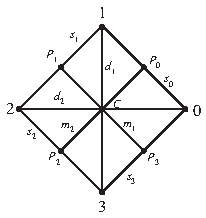
\includegraphics[width=0.282\linewidth,height=.8\textheight,keepaspectratio]{assets/p151_00.pdf}\end{center}
\begin{center}\small\textbf{14.10 Figure}\end{center}
\end{BookFloat}

We can think of the set

\begin{center}\begin{adjustbox}{max width=\linewidth}\BookInline{\displaystyle X= \{0,\allowbreak 1,\allowbreak 2,\allowbreak 3,\allowbreak s_{0},\allowbreak s_{1},\allowbreak s_{2},\allowbreak s_{3},\allowbreak m_{1},\allowbreak m_{2},\allowbreak d_{1},\allowbreak d_{2},\allowbreak C,\allowbreak P_{0},\allowbreak P_{1},\allowbreak P_{2},\allowbreak P_{3}\}}\end{adjustbox}\end{center}

\noindent as a \BookInline{D_{4}-}set in a natural way. Table 14.11 shows the action of \BookInline{D_{4}} on \BookInline{X.} Recall that \BookInline{\iota } is the identity\BookInline{,\allowbreak \rho ^{k}} is rotation by \BookInline{k\pi /2,\allowbreak } and \BookInline{\mu } is reflection across the line \BookInline{d_{2}.} We can see from the table that \BookInline{\mu \rho } is reflection across the line \BookInline{m_{1},\allowbreak \mu \rho ^{2}} is reflection across the line \BookInline{d_{1},\allowbreak } and \BookInline{\mu \rho ^{3}} is reflection across the line \BookInline{m_{2}.} It is worthwhile to spend a little time to understand how Table 14.11 was constructed before continuing\BookInline{.}\BookEnd{\blacktriangle}

\begin{BookFloat}{14_group_action_on_a_set-p151-4}
\BookStatement{\textbf{14.11 Table}}
\begin{center}\begin{adjustbox}{max width=\linewidth}\small\setlength{\tabcolsep}{3pt}
\begin{tabular}{c|ccccccccccccccccc}
\hline
 & \BookInline{0} & \BookInline{1} & \BookInline{2} & \BookInline{3} & \BookInline{s_0} & \BookInline{s_1} & \BookInline{s_2} & \BookInline{s_3} & \BookInline{m_1} & \BookInline{m_2} & \BookInline{d_1} & \BookInline{d_2} & \BookInline{C} & \BookInline{P_0} & \BookInline{P_1} & \BookInline{P_2} & \BookInline{P_3}\\\hline
\BookInline{\iota} & \BookInline{0} & \BookInline{1} & \BookInline{2} & \BookInline{3} & \BookInline{s_0} & \BookInline{s_1} & \BookInline{s_2} & \BookInline{s_3} & \BookInline{m_1} & \BookInline{m_2} & \BookInline{d_1} & \BookInline{d_2} & \BookInline{C} & \BookInline{P_0} & \BookInline{P_1} & \BookInline{P_2} & \BookInline{P_3}\\
\BookInline{\rho} & \BookInline{1} & \BookInline{2} & \BookInline{3} & \BookInline{0} & \BookInline{s_1} & \BookInline{s_2} & \BookInline{s_3} & \BookInline{s_0} & \BookInline{m_2} & \BookInline{m_1} & \BookInline{d_2} & \BookInline{d_1} & \BookInline{C} & \BookInline{P_1} & \BookInline{P_2} & \BookInline{P_3} & \BookInline{P_0}\\
\BookInline{\rho^2} & \BookInline{2} & \BookInline{3} & \BookInline{0} & \BookInline{1} & \BookInline{s_2} & \BookInline{s_3} & \BookInline{s_0} & \BookInline{s_1} & \BookInline{m_1} & \BookInline{m_2} & \BookInline{d_1} & \BookInline{d_2} & \BookInline{C} & \BookInline{P_2} & \BookInline{P_3} & \BookInline{P_0} & \BookInline{P_1}\\
\BookInline{\rho^3} & \BookInline{3} & \BookInline{0} & \BookInline{1} & \BookInline{2} & \BookInline{s_3} & \BookInline{s_0} & \BookInline{s_1} & \BookInline{s_2} & \BookInline{m_2} & \BookInline{m_1} & \BookInline{d_2} & \BookInline{d_1} & \BookInline{C} & \BookInline{P_3} & \BookInline{P_0} & \BookInline{P_1} & \BookInline{P_2}\\
\BookInline{\mu} & \BookInline{0} & \BookInline{3} & \BookInline{2} & \BookInline{1} & \BookInline{s_3} & \BookInline{s_2} & \BookInline{s_1} & \BookInline{s_0} & \BookInline{m_1} & \BookInline{m_2} & \BookInline{d_2} & \BookInline{d_1} & \BookInline{C} & \BookInline{P_3} & \BookInline{P_2} & \BookInline{P_1} & \BookInline{P_0}\\
\BookInline{\mu\rho} & \BookInline{3} & \BookInline{2} & \BookInline{1} & \BookInline{0} & \BookInline{s_2} & \BookInline{s_1} & \BookInline{s_0} & \BookInline{s_3} & \BookInline{m_2} & \BookInline{m_1} & \BookInline{d_1} & \BookInline{d_2} & \BookInline{C} & \BookInline{P_2} & \BookInline{P_1} & \BookInline{P_0} & \BookInline{P_3}\\
\BookInline{\mu\rho^2} & \BookInline{2} & \BookInline{1} & \BookInline{0} & \BookInline{3} & \BookInline{s_1} & \BookInline{s_0} & \BookInline{s_3} & \BookInline{s_2} & \BookInline{m_1} & \BookInline{m_2} & \BookInline{d_2} & \BookInline{d_1} & \BookInline{C} & \BookInline{P_1} & \BookInline{P_0} & \BookInline{P_3} & \BookInline{P_2}\\
\BookInline{\mu\rho^3} & \BookInline{1} & \BookInline{0} & \BookInline{3} & \BookInline{2} & \BookInline{s_0} & \BookInline{s_3} & \BookInline{s_2} & \BookInline{s_1} & \BookInline{m_2} & \BookInline{m_1} & \BookInline{d_1} & \BookInline{d_2} & \BookInline{C} & \BookInline{P_0} & \BookInline{P_3} & \BookInline{P_2} & \BookInline{P_1}\\
\hline\end{tabular}\end{adjustbox}\end{center}
\end{BookFloat}

\BookTextHeading{\textbf{Isotropy Subgroups}  }

\noindent Let \BookInline{X} be a \BookInline{G-}set. Let \BookInline{x\in X} and \BookInline{g\in G.} It will be important to know when \BookInline{gx= x.} We let

\begin{center}\begin{adjustbox}{max width=\linewidth}\BookInline{\displaystyle X_{g}= \{x\in X\mid gx= x\}\;\text{and}\;G_{x}= \{g\in G\mid gx= x\}.}\end{adjustbox}\end{center}

\BookLabel{14.12 Example} For the \BookInline{D_{4}-}set \BookInline{X} in Example 14.9, we have

\begin{center}\begin{adjustbox}{max width=\linewidth}\BookInline{\displaystyle X_{\iota }= X,\allowbreak }\end{adjustbox}\end{center}

\begin{center}\begin{adjustbox}{max width=\linewidth}\BookInline{\displaystyle X_{\rho }= \{C\},\allowbreak }\end{adjustbox}\end{center}

\begin{center}\begin{adjustbox}{max width=\linewidth}\BookInline{\displaystyle X_{\mu }= \{0,\allowbreak 2,\allowbreak d_{1},\allowbreak d_{2},\allowbreak C\}.}\end{adjustbox}\end{center}

Also, using the same \BookInline{D_{4}} action on \BookInline{X,\allowbreak }

\begin{center}\begin{adjustbox}{max width=\linewidth}\BookInline{\displaystyle G_{0}= \{\iota ,\allowbreak \mu \},\allowbreak }\end{adjustbox}\end{center}

\begin{center}\begin{adjustbox}{max width=\linewidth}\BookInline{\displaystyle G_{s_{2}}= \{\iota ,\allowbreak \mu \rho ^{3}\},\allowbreak }\end{adjustbox}\end{center}

\begin{center}\begin{adjustbox}{max width=\linewidth}\BookInline{\displaystyle G_{d_{1}}= \{\iota ,\allowbreak \rho ^{2},\allowbreak \mu ,\allowbreak \mu \rho ^{2}\}.}\end{adjustbox}\end{center}

We leave the computations of the other sets of the form \BookInline{X_{\sigma }} and \BookInline{G_{x}} to Exercises 1 and \BookInline{2.}\BookEnd{\blacktriangle}

Note that the subsets \BookInline{G_{x}} given in the preceding example were, in each case, subgroups of \BookInline{G.} This is true in general.

\end{BookBody}

% Source PDF page 152; original printed page 135
\BookSource{152}{135}
\BookNarrativetrue

\begin{BookBody}

\BookLabel{14.13 Theorem} Let \BookInline{X} be a \BookInline{G-}set. Then \BookInline{G_{x}} is a subgroup of \BookInline{G} for each \BookInline{x\in X.}

\BookLabel{\textit{Proof}} Let \BookInline{x\in X} and let \BookInline{g_{1},\allowbreak g_{2}\in G_{x}.} Then \BookInline{g_{1}x= x} and \BookInline{g_{2}x= x.} Consequently\BookInline{,\allowbreak (g_{1}g_{2})x= } \BookInline{g_{1}(g_{2}x)= g_{1}x= x,\allowbreak } so \BookInline{g_{1}g_{2}\in G_{x},\allowbreak } and \BookInline{G_{x}} is closed under the induced operation of \BookInline{G.} Of course,\textit{ ex} \BookInline{= x,\allowbreak } so \BookInline{e\in G_{x}.} If \BookInline{g\in G_{x},\allowbreak } then \BookInline{gx= x,\allowbreak } so \BookInline{x= } \textit{ex} \BookInline{= (g^{- 1}g)x= g^{- 1}(gx)= } \BookInline{g^{- 1}x,\allowbreak } and consequently \BookInline{g^{- 1}\in G_{x}.} Thus \BookInline{G_{x}} is a subgroup of \BookInline{G.}\BookEnd{\blacklozenge}

\BookLabel{14.14 Definition} Let \BookInline{X} be a \BookInline{G-}set and let \BookInline{x\in X.} The subgroup \BookInline{G_{x}} is the\textbf{ isotropy subgroup of} \BookInline{x.}\BookEnd{\blacksquare}

\BookTextHeading{\textbf{Orbits}}

\noindent For the \BookInline{D_{4}-}set \BookInline{X} of Example 14.9 with action table in Table 14.11, the elements in the subset \BookInline{\{0,\allowbreak 1,\allowbreak 2,\allowbreak 3\}} are carried into elements of this same subset under action by \BookInline{D_{4}.} Furthermore, each of the elements 0, 1, 2, and 3 is carried into all the other elements of the subset by the various elements of \BookInline{D_{4}.} We proceed to show that every \BookInline{G-}set \BookInline{X} can be partitioned into subsets of this type.

\BookLabel{14.15 Theorem} Let \BookInline{X} be a \BookInline{G-}set. For \BookInline{x_{1},\allowbreak x_{2}\in X,\allowbreak } let \BookInline{x_{1}\sim x_{2}} if and only if there exists \BookInline{g\in G} such that \BookInline{gx_{1}= x_{2}.} Then \BookInline{\sim } is an equivalence relation on \BookInline{X.}

\BookLabel{\textit{Proof}} For each \BookInline{x\in X,\allowbreak } we have\textit{ ex} \BookInline{= x,\allowbreak } so \BookInline{x\sim x} and \BookInline{\sim } is reflexive.

Suppose \BookInline{x_{1}\sim x_{2},\allowbreak } so \BookInline{gx_{1}= x_{2}} for some \BookInline{g\in G.} Then \BookInline{g^{- 1}x_{2}= g^{- 1}(gx_{1})= } \BookInline{(g^{- 1}g)x_{1}= ex_{1}= x_{1},\allowbreak } so \BookInline{x_{2}\sim x_{1},\allowbreak } and \BookInline{\sim } is symmetric.

Finally, if \BookInline{x_{1}\sim x_{2}} and \BookInline{x_{2}\sim x_{3},\allowbreak } then \BookInline{g_{1}x_{1}= x_{2}} and \BookInline{g_{2}x_{2}= x_{3}} for some \BookInline{g_{1},\allowbreak g_{2}\in G.} Then \BookInline{(g_{2}g_{1})x_{1}= g_{2}(g_{1}x_{1})= g_{2}x_{2}= x_{3},\allowbreak } so \BookInline{x_{1}\sim x_{3}} and \BookInline{\sim } is transitive\BookInline{.}\BookEnd{\blacklozenge}

\BookLabel{14.16 Definition} Let \BookInline{X} be a \BookInline{G-}set. Each cell in the partition of the equivalence relation described in Theorem 14.15 is an\textbf{ orbit in} \BookInline{X} \textbf{under} \BookInline{G.} If \BookInline{x\in X,\allowbreak } the cell containing \BookInline{x} is the\textbf{ orbit} \textbf{of} \BookInline{x.} We let this cell be \BookInline{Gx.}\BookEnd{\blacksquare}

The relationship between the orbits in \BookInline{X} and the group structure of \BookInline{G} lies at the heart of many applications. The following theorem gives this relationship. Recall that for a set \BookInline{X,\allowbreak } we use \BookInline{|X|} for the number of elements in \BookInline{X,\allowbreak } and \BookInline{(G:H)} is the index of a subgroup \BookInline{H} in a group \BookInline{G.}

\BookLabel{14.17 Theorem} Let \BookInline{X} be a \BookInline{G-}set and let \BookInline{x\in X.} Then \BookInline{|Gx|= (G:G_{x}).} If \BookInline{|G|} is finite, then \BookInline{|Gx|} is a divisor of \BookInline{|G|.}

\BookLabel{\textit{Proof}} We define a one-to-one map \BookInline{\psi } from \BookInline{Gx} onto the collection of left cosets of \BookInline{G_{x}} in \BookInline{G.} Let \BookInline{x_{1}\in Gx.} Then there exists \BookInline{g_{1}\in G} such that \BookInline{g_{1}x= x_{1}.} We define \BookInline{\psi (x_{1})} to be the left coset \BookInline{g_{1}G_{x}} of \BookInline{G_{x}.} We must show that this map \BookInline{\psi } is well defined, independent of the choice of \BookInline{g_{1}\in G} such that \BookInline{g_{1}x= x_{1}.} Suppose also that \BookInline{g_{1}^{\prime }x= x_{1}.} Then\BookInline{,\allowbreak g_{1}x= g_{1}^{\prime }x,\allowbreak } so \BookInline{g_{1}^{- 1}(g_{1}x)= g_{1}^{- 1}(g_{1}^{\prime }x),\allowbreak } from which we deduce \BookInline{x= (g_{1}^{- 1}g_{1}^{\prime })x.} Therefore \BookInline{g_{1}^{- 1}g_{1}^{\prime }\in G_{x},\allowbreak } so \BookInline{g_{1}^{\prime }\in g_{1}G_{x},\allowbreak } and \BookInline{g_{1}G_{x}= g_{1}^{\prime }G_{x}.} Thus the map \BookInline{\psi } is well defined.

To show the map \BookInline{\psi } is one-to-one, suppose \BookInline{x_{1},\allowbreak x_{2}\in Gx,\allowbreak } and \BookInline{\psi (x_{1})= \psi (x_{2}).} Then there exist \BookInline{g_{1},\allowbreak g_{2}\in G} such that \BookInline{x_{1}= g_{1}x,\allowbreak x_{2}= g_{2}x,\allowbreak } and \BookInline{g_{2}\in g_{1}G_{x}.} Then \BookInline{g_{2}= g_{1}g} for some \BookInline{g\in G_{x},\allowbreak } so \BookInline{x_{2}= g_{2}x= g_{1}(gx)= g_{1}x= x_{1}.} Thus \BookInline{\psi } is one-to-one.

Finally, we show that each left coset of \BookInline{G_{x}} in \BookInline{G} is of the form \BookInline{\psi (x_{1})} for some \BookInline{x_{1}\in Gx.} Let \BookInline{g_{1}G_{x}} be a left coset. Then if \BookInline{g_{1}x= x_{1},\allowbreak } we have \BookInline{g_{1}G_{x}= \psi (x_{1}).} Thus \BookInline{\psi } maps \BookInline{Gx} one-to-one onto the collection of left cosets so \BookInline{|Gx|= (G:G_{x}).}

If \BookInline{|G|} is finite, then the equation \BookInline{|G|= |G_{x}|(G:G_{x})} shows that \BookInline{|Gx|= (G:G_{x})} is a divisor of \BookInline{|G|.}\BookEnd{\blacklozenge}

\end{BookBody}

% Source PDF page 153; original printed page 136
\BookSource{153}{136}
\BookNarrativetrue

\begin{BookBody}

\BookLabel{14.18 Example} Let \BookInline{X} be the \BookInline{D_{4}-}set in Example 14.9, with action table given by Table 14.11. With \BookInline{G= D_{4},\allowbreak } we have \BookInline{G_{0}= \{\iota,\allowbreak \mu \}.} Since \BookInline{|G|= 8,\allowbreak } we have \BookInline{|G0|= (G:G_{0})= 4.} From Table 14.11, we see that \BookInline{G0= \{0,\allowbreak 1,\allowbreak 2,\allowbreak 3\},\allowbreak } which indeed has four elements\BookInline{.}\BookEnd{\blacktriangle}

We should remember not only the cardinality equation in Theorem 14.17 but also that the\textit{ elements of} \BookInline{G} \textit{carrying} \BookInline{x} \textit{into} \BookInline{g_{1}x} \textit{are precisely the elements of the left coset} \BookInline{g_{1}G_{x}.} Namely, if \BookInline{g\in G_{x},\allowbreak } then \BookInline{(g_{1}g)x= g_{1}(gx)= g_{1}x.} On the other hand, if \BookInline{g_{2}x= g_{1}x,\allowbreak } then \BookInline{g_{1}^{- 1}(g_{2}x)= x} so \BookInline{(g_{1}^{- 1}g_{2})x= x.} Thus \BookInline{g_{1}^{- 1}g_{2}\in G_{x}} so \BookInline{g_{2}\in g_{1}G_{x}.}

\BookTextHeading{\textbf{Applications of} \textit{\textbf{G}}\textbf{-Sets to Finite Groups}    }

\noindent Theorem 14.17 is a very useful theorem in the study of finite groups. Suppose that \BookInline{X} is a \BookInline{G-}set for a finite group \BookInline{G} and we pick out one element from each orbit of \BookInline{X} to make the set \BookInline{S= \{x_{1},\allowbreak x_{2},\allowbreak...,\allowbreak x_{r}\}} where we indexed the elements of \BookInline{X} so that if \BookInline{i\leq j,\allowbreak } then \BookInline{|Gx_{i}|\geq |Gx_{j}|.} That is, we arrange by orbit size, largest first and smallest last. Every element in \BookInline{X} is in precisely one orbit, so

\begin{center}\begin{adjustbox}{max width=\linewidth}\BookInline{\displaystyle |X|= \sum _{i= 1}^{r}|Gx_{i}|.(1)}\end{adjustbox}\end{center}

\noindent We let \BookInline{X_{G}= \{x\in X\mid gx= x} for all \BookInline{g\in G\}.} That is\BookInline{,\allowbreak X_{G}} is the set of all elements of \BookInline{X} whose orbit size is 1. So by equation (1),

\begin{center}\begin{adjustbox}{max width=\linewidth}\BookInline{\displaystyle |X|= |X_{G}|+ \sum _{i= 1}^{s}|Gx_{i}|(2)}\end{adjustbox}\end{center}

\noindent where we simply place all the orbits with one element into \BookInline{X_{G}} and we are left with \BookInline{s} orbits each containing at least two elements. Although Equation (2) is simply saying that if you add up the sizes of all the orbits you account for all the elements of \BookInline{X,\allowbreak } when coupled with Theorem 14.17, it gives some very interesting results. We give a few in the remainder of this section. In Section 17 we will use Equation 2 extensively to prove the Sylow Theorems.

For the remainder of this section,\textit{ we assume that} \BookInline{p} \textit{is} \BookInline{a} \textit{prime number}.

\BookLabel{14.19 Theorem} Let \BookInline{G} be a group with \BookInline{p^{n}} elements. If \BookInline{X} is a \BookInline{G-}set, then \BookInline{|X|\equiv |X_{G}|} mod \BookInline{p.}

\BookLabel{\textit{Proof}} Using Equation 2,

\begin{center}\begin{adjustbox}{max width=\linewidth}\BookInline{\displaystyle |X|= |X_{G}|+ \sum _{i= 1}^{s}|Gx_{i}|.}\end{adjustbox}\end{center}

\noindent Since for each \BookInline{i\leq s,\allowbreak |Gx_{i}|\geq 2} and \BookInline{|Gx_{i}|= (G:G_{x_{i}})} is a divisor of \BookInline{|G|= p^{n},\allowbreak } by Theorem \BookInline{14.17p} divides each term in the sum \BookInline{\sum _{i= 1}^{s}|Gx_{i}|.} Thus \BookInline{|X|\equiv |X_{G}|} mod \BookInline{p.}\BookEnd{\blacklozenge}

\noindent Knowing that \BookInline{k} divides the order of a group is not sufficient information to assume that the group has a subgroup of order \BookInline{k.} For example, we saw that \BookInline{A_{4}} has no subgroup of order 6 and that in general\BookInline{,\allowbreak A_{n}} has no subgroup of index 2 if \BookInline{n\geq 4.} On the positive side, in Exercise 29 in Section 2, you were asked to show that if a group has an even number of elements, then it has an element of order two. Theorem 14.20 generalizes this result to show that if a prime number \BookInline{p} divides the order of a group, then the group has an element of order \BookInline{p.} The proof of this theorem relies on Theorem 14.19.

\BookLabel{14.20 Theorem} \textbf{(Cauchy’s Theorem)} Let \BookInline{G} be a group such that \BookInline{p} divides the order of \BookInline{G.} Then \BookInline{G} has an element of order \BookInline{p} and therefore a subgroup of order \BookInline{p.}

\end{BookBody}

% Source PDF page 154; original printed page 137
\BookSource{154}{137}
\BookNarrativetrue

\begin{BookBody}

\BookLabel{\textit{Proof}} We let

\begin{center}\begin{adjustbox}{max width=\linewidth}\BookInline{\displaystyle X= \{(g_{0},\allowbreak g_{1},\allowbreak g_{2},\allowbreak ...,\allowbreak g_{p- 1})\mid g_{0},\allowbreak g_{1},\allowbreak ...,\allowbreak g_{p- 1}\in G\;\text{and}\;g_{0}g_{1}g_{2}...g_{p- 1}= e\}.}\end{adjustbox}\end{center}

\noindent That is\BookInline{,\allowbreak X} is the set of all \BookInline{p-}tuples with entries in \BookInline{G} so that when the entries are multiplied together (in order) their product is the identity \BookInline{e.} Since the product is \BookInline{e,\allowbreak g_{0}= } \BookInline{(g_{1}g_{2}...g_{p- 1})^{- 1}} and given any \BookInline{g_{1},\allowbreak g_{2},\allowbreak...,\allowbreak g_{p- 1}\in G,\allowbreak } by picking \BookInline{g_{0}= (g_{1}g_{2}...g_{p- 1})^{- 1}} we have an element in \BookInline{X.} Thus \BookInline{|X|= |G|^{p- 1}} and in particular\BookInline{,\allowbreak p} divides the order of \BookInline{X} since \BookInline{p} divides the order of \BookInline{G.}

\begingroup\sloppy Suppose that \BookInline{(g_{0},\allowbreak g_{1},\allowbreak g_{2},\allowbreak...,\allowbreak g_{p- 1})\in X.} Since \BookInline{g_{0}= (g_{1}g_{2}...g_{p- 1})^{- 1},\allowbreak } it follows that \BookInline{(g_{1},\allowbreak g_{2},\allowbreak...g_{p- 1},\allowbreak g_{0})} is in \BookInline{X.} Repeating this process, noting that \BookInline{g_{1}= (g_{2}g_{3}...g_{p- 1}g_{0})^{- 1}} we conclude that \BookInline{(g_{2},\allowbreak g_{3},\allowbreak g_{4},\allowbreak \cdots,\allowbreak g_{p- 1},\allowbreak g_{0},\allowbreak g_{1})\in X.} Continuing in this manner we have that for any \BookInline{k\in \mathbb{Z}_{p},\allowbreak }\par\endgroup

\begin{center}\begin{adjustbox}{max width=\linewidth}\BookInline{\displaystyle (g_{k},\allowbreak g_{k+ _{p}1},\allowbreak g_{k+ _{p}2},\allowbreak ...,\allowbreak g_{k+ _{p}(p- 1)})\in X.}\end{adjustbox}\end{center}

\noindent We check that this gives a group action of \BookInline{\mathbb{Z}_{p}} on \BookInline{X.} Let \BookInline{k\in \mathbb{Z}_{p}} and \BookInline{(g_{0},\allowbreak g_{1},\allowbreak g_{2},\allowbreak...,\allowbreak g_{p- 1})\in } \BookInline{X.} Then

\begin{center}\begin{adjustbox}{max width=\linewidth}\BookInline{\displaystyle k(g_{0},\allowbreak g_{1},\allowbreak g_{2},\allowbreak ...,\allowbreak g_{p- 1})= (g_{k},\allowbreak g_{k+ _{p}1},\allowbreak g_{k+ _{p}2},\allowbreak ...,\allowbreak g_{k+ _{p}(p- 1)})\in X.}\end{adjustbox}\end{center}

\noindent Since

\begin{center}\begin{adjustbox}{max width=\linewidth}\BookInline{\displaystyle 0(g_{0},\allowbreak g_{1},\allowbreak g_{2},\allowbreak ...,\allowbreak g_{p- 1})= (g_{0},\allowbreak g_{1},\allowbreak g_{2},\allowbreak ...,\allowbreak g_{p- 1})\;\text{and}\;}\end{adjustbox}\end{center}

\begin{center}\begin{adjustbox}{max width=\linewidth}\BookInline{\displaystyle \begin{aligned}k(l(g_{0},\allowbreak g_{1},\allowbreak g_{2},\allowbreak ...,\allowbreak g_{p- 1}))&= k(g_{l},\allowbreak g_{l+ _{p}1},\allowbreak g_{l+ _{p}2},\allowbreak ...,\allowbreak g_{l+ _{p}(p- 1)}) \\ &= (g_{k+ _{p}l},\allowbreak g_{k+ _{p}l+ _{p}1},\allowbreak ...,\allowbreak g_{k+ _{p}l+ _{p}(p- 1)}) \\ &= (k+ _{p}l)(g_{0},\allowbreak g_{1},\allowbreak g_{2},\allowbreak ...,\allowbreak g_{p- 1})\end{aligned}}\end{adjustbox}\end{center}

\noindent this is indeed a group action.

By Theorem 14. \BookInline{19,\allowbreak 0\equiv |X|\equiv |X_{\mathbb{Z}_{p}}|} mod \BookInline{p.} The \BookInline{p-}tuple \BookInline{(e,\allowbreak e,\allowbreak e,\allowbreak...,\allowbreak e)} is in \BookInline{X_{\mathbb{Z}_{p}}} because rearranging the entries does not change the \BookInline{p-}tuple. Since \BookInline{X_{\mathbb{Z}_{p}}} contains at least one element and \BookInline{p} divides \BookInline{|X_{\mathbb{Z}_{p}}|,\allowbreak X_{\mathbb{Z}_{p}}} must contain at least one element other than \BookInline{(e,\allowbreak e,\allowbreak e,\allowbreak...,\allowbreak e).} That element must have the form \BookInline{(a,\allowbreak a,\allowbreak a,\allowbreak...,\allowbreak a)} with \BookInline{a\neq e} and \BookInline{a^{p}= e.} So \BookInline{a} has order \BookInline{p} and the subgroup it generates is a subgroup of \BookInline{G} with order \BookInline{p.}\BookEnd{\blacklozenge}

\BookLabel{14.21 Definition} A \BookInline{p-}group is a group such that each element in the group has order a power of \BookInline{p.} A \BookInline{p-}subgroup of a group is a subgroup that is a \BookInline{p-}group\BookInline{.}\BookEnd{\blacksquare}

\BookLabel{14.22 Example} The group \BookInline{D_{16}} is a 2-group since the order of any element of \BookInline{D_{16}} divides \BookInline{|D_{16}|= 32.} \BookEnd{\blacktriangle}

\BookLabel{14.23 Example} Using the Fundamental Theorem of Finitely Generated Abelian Groups, a finite abelian group is a \BookInline{p-}group if and only if it is isomorphic to

\begin{center}\begin{adjustbox}{max width=\linewidth}\BookInline{\displaystyle \mathbb{Z}_{p^{1}}^{r}\times \mathbb{Z}_{p^{2}}^{r}\times \mathbb{Z}_{p^{3}}^{r}\times \cdots \times \mathbb{Z}_{p}rn.}\end{adjustbox}\end{center}

\noindent This is because if there were a factor of the form \BookInline{\mathbb{Z}_{q}s} where \BookInline{q\neq p} is a prime number and \BookInline{s\geq 1,\allowbreak } then there would be an element in \BookInline{G} with order \BookInline{q^{s}} which is not a power of \BookInline{p.}

In Exercise 30, you are asked to show that for \BookInline{G} a finite group\BookInline{,\allowbreak G} is a \BookInline{p-}group if and only if the order of \BookInline{G} is a power of \BookInline{p.}

The next theorem assures us that any finite \BookInline{p-}group has a nontrivial normal subgroup, namely the center of the group\BookInline{.}\BookEnd{\blacktriangle}

\BookLabel{14.24 Theorem} Let \BookInline{G} be a finite \BookInline{p-}group. Then the center of \BookInline{G,\allowbreak Z(G),\allowbreak } is not the trivial group.

\BookLabel{\textit{Proof}} We let \BookInline{X= G} and we make \BookInline{X} into a \BookInline{G-}set using conjugation. That is\BookInline{,\allowbreak \ast (g,\allowbreak a)= gag^{- 1}.} Equation 2 states that \BookInline{0\equiv |X|\equiv |X_{G}|} mod \BookInline{p.} For all \BookInline{g\in G,\allowbreak geg^{- 1}= e.} So \BookInline{X_{G}} has at 
% Source PDF page 155; original printed page 138
\BookSource{155}{138}
least one element, namely \BookInline{e.} Since the number of elements in \BookInline{X_{G}} must be at least \BookInline{p,\allowbreak } there is an element \BookInline{a\in X} such that \BookInline{a\neq e} and \BookInline{gag^{- 1}= a} for all \BookInline{g\in G.} Thus \BookInline{ga= ag} for all \BookInline{g\in G,\allowbreak } which says that \BookInline{a\in Z(G).} So \BookInline{Z(G)} is not the trivial subgroup\BookInline{.}\BookEnd{\blacklozenge}

\end{BookBody}

\BookNarrativetrue

\begin{BookBody}

\noindent When studying \BookInline{p-}groups, the fact that the center is nontrivial is often very helpful. We conclude this section with a theorem that illustrates the utility of Theorem 14.24.

\BookLabel{14.25 Theorem} Every group of order \BookInline{p^{2}} is abelian.

\BookLabel{\textit{Proof}} Let \BookInline{G} be a group of order \BookInline{p^{2}} with center \BookInline{Z(G).} By Theorem \BookInline{14.24,\allowbreak Z(G)} is not the trivial group so it is either all of \BookInline{G} or else it has order \BookInline{p.} We wish to show that \BookInline{Z(G)= G} using proof by contradiction. So we assume that \BookInline{Z(G)} has \BookInline{p} elements. Since \BookInline{Z(G)} is a normal subgroup of \BookInline{G,\allowbreak } we can form \BookInline{G/Z(G).} The group \BookInline{G/Z(G)} also has \BookInline{p} elements and so both \BookInline{Z(G)} and \BookInline{G/Z(G)} are cyclic. Let \BookInline{\langle a\rangle = Z(G)} and \BookInline{\langle bZ(G)\rangle = G/Z(G).} Let \BookInline{x,\allowbreak y\in G.} Then \BookInline{x= b^{i}a^{j}} and \BookInline{y= b^{r}a^{s}} for some integers \BookInline{i,\allowbreak j,\allowbreak r,\allowbreak s} since the cosets of \BookInline{Z(G)} partition \BookInline{G.} Then

\begin{center}\begin{adjustbox}{max width=\linewidth}\BookInline{\displaystyle xy= b^{i}a^{j}b^{r}a^{s}= b^{i}b^{r}a^{j}a^{s}}\end{adjustbox}\end{center}

\noindent since \BookInline{\langle a\rangle } is the center of \BookInline{G.} So

\begin{center}\begin{adjustbox}{max width=\linewidth}\BookInline{\displaystyle xy= b^{i+ r}a^{j+ s}= b^{r}b^{i}a^{s}a^{j}= b^{r}a^{s}b^{i}a^{j}= yx.}\end{adjustbox}\end{center}

\noindent Since every element in \BookInline{G} commutes with every other element\BookInline{,\allowbreak Z(G)= G,\allowbreak } which contradicts our assumption that the center has only \BookInline{p} elements. So the center of \BookInline{G} must be \BookInline{G,\allowbreak } which means that \BookInline{G} is abelian\BookInline{.}\BookEnd{\blacklozenge}

\BookLabel{14.26 Example} Since every group of order \BookInline{p^{2}} is abelian, the Fundamental Homomorphism Theorem says that every group with \BookInline{p^{2}} elements is isomorphic to either \BookInline{\mathbb{Z}_{p}2\;\text{or}\;\mathbb{Z}_{p}\times \mathbb{Z}_{p}.} The two groups of order 4 are \BookInline{\mathbb{Z}_{4}} and the Klein 4-group. The two groups of order 9 are \BookInline{\mathbb{Z}_{9}} and \BookInline{\mathbb{Z}_{3}\times \mathbb{Z}_{3}.}\BookEnd{\blacktriangle}

\end{BookBody}

\BookNarrativefalse

\begin{BookBody}

\BookExerciseTitle{14}

\BookTextHeading{\textbf{Computations}}

\noindent In Exercises 1 through 3, let

\begin{center}\begin{adjustbox}{max width=\linewidth}\BookInline{\displaystyle X= \{0,\allowbreak 1,\allowbreak 2,\allowbreak 3,\allowbreak s_{0},\allowbreak s_{1},\allowbreak s_{2},\allowbreak s_{3},\allowbreak m_{1},\allowbreak m_{2},\allowbreak d_{1},\allowbreak d_{2},\allowbreak C,\allowbreak P_{0},\allowbreak P_{1},\allowbreak P_{2},\allowbreak P_{3}\}}\end{adjustbox}\end{center}

\noindent be the \BookInline{D_{4}-}set of Example 14.9. Find the following, where \BookInline{G= D_{4}.}

\BookExercise{1.}{The fixed sets \BookInline{X_{\sigma }} for each \BookInline{\sigma \in D_{4}.}}

\BookExercise{2.}{The isotropy subgroups \BookInline{G_{x}} for each \BookInline{x\in X,\allowbreak } that is\BookInline{,\allowbreak G_{0},\allowbreak G_{1},\allowbreak \cdots,\allowbreak G_{P_{2}},\allowbreak G_{P_{3}}.}}

\BookExercise{3.}{The orbits in \BookInline{X} under \BookInline{D_{4}.}}

\BookExercise{4.}{Theorem 14.24 states that every \BookInline{p-}group has nontrivial center. Find the center of \BookInline{D_{8}.}}

\BookExercise{5.}{Find the center of \BookInline{D_{7}.}}

\BookExercise{6.}{Let \BookInline{G= X= S_{3}} and make \BookInline{X} a \BookInline{G-}set using conjugation. That is\BookInline{,\allowbreak \ast (\sigma,\allowbreak \tau )= \sigma \tau \sigma ^{- 1}.} Find all the orbits of \BookInline{X} using this action. (Write permutations in disjoint cycle notation.)}

\BookExercise{7.}{Let \BookInline{G= D_{4}} and \BookInline{X} be the set of all subgroups of \BookInline{D_{4}} with order two. The set \BookInline{X} is a \BookInline{G-}set using conjugation, \BookInline{\ast (\sigma,\allowbreak H)= \sigma H\sigma ^{- 1}.} Find all the orbits of this group action.}

\BookExercise{8.}{Let \BookInline{G= U= \{z\in \mathbb{C}\mid |z|= 1\}} be the circle group. Then \BookInline{X= \mathbb{C},\allowbreak } the set of complex numbers, is a \BookInline{G-}set with group action given by complex number multiplication. That is, if \BookInline{z\in U} and \BookInline{w\in \mathbb{C},\allowbreak \ast (z,\allowbreak w)= zw.} Find all the orbits of this action. Also, find \BookInline{X_{G}.}}

\end{BookBody}

% Source PDF page 156; original printed page 139
\BookSource{156}{139}
\BookNarrativefalse

\begin{BookBody}

\BookExercise{9.}{Let \BookInline{G} be a group of order 3 and suppose that \BookInline{|X|= 6.} For each possible action of \BookInline{G} on \BookInline{X,\allowbreak } give a list of the orbit sizes. List the orbit sizes from largest to smallest. (Recall that the orbits partition the set \BookInline{X.)}}

\BookExercise{10.}{Let \BookInline{G} be a group of order 9 and suppose that \BookInline{|X|= 10.} For each possible action of \BookInline{G} on \BookInline{X,\allowbreak } give a list of the orbit sizes. List the orbit sizes from largest to smallest.}

\BookExercise{11.}{Let \BookInline{G} be a group of order 8 and suppose that \BookInline{|X|= 10.} For each possible way to make \BookInline{X} a \BookInline{G-}set the orbits partition \BookInline{X.} For each possible action of \BookInline{G} on \BookInline{X,\allowbreak } give a list of the orbit sizes. List the orbit sizes from largest to smallest.}

\BookTextHeading{\textbf{Concepts}}

\noindent In Exercises 12 and 13, correct the definition of the italicized term without reference to the text, if correction is needed, so that it is in a form acceptable for publication.

\BookExercise{12.}{A group \BookInline{G} \textit{acts faithfully} on \BookInline{X} if and only if \BookInline{gx= x} implies that \BookInline{g= e.}}

\BookExercise{13.}{A group \BookInline{G} is\textit{ transitive} on a \BookInline{G-}set \BookInline{X} if and only if, for some \BookInline{g\in G,\allowbreak gx} can be every other \BookInline{x.}}

\BookExercise{14.}{Let \BookInline{X} be a \BookInline{G-}set and let \BookInline{S\subseteq X.} If \BookInline{Gs\subseteq S} for all \BookInline{s\in S,\allowbreak } then \BookInline{S} is a\textbf{ sub}\BookInline{-G-}\textbf{set.} Characterize a sub\BookInline{-G-}set of a \BookInline{G-}set \BookInline{X} in terms of orbits in \BookInline{X} under \BookInline{G.}}

\BookExercise{15.}{Characterize a transitive \BookInline{G-}set in terms of its orbits.}

\BookExercise{16.}{Determine whether each of the following is true or false.}

\BookExercise{a.}{Every \BookInline{G-}set is also a group.}

\BookExercise{b.}{Each element of a \BookInline{G-}set is fixed by the identity of \BookInline{G.}}

\BookExercise{c.}{If every element of a \BookInline{G-}set is fixed by the same element \BookInline{g} of \BookInline{G,\allowbreak } then \BookInline{g} must be the identity \BookInline{e.}}

\BookExercise{d.}{Let \BookInline{X} be a \BookInline{G-}set with \BookInline{x_{1},\allowbreak x_{2}\in X} and \BookInline{g\in G.} If \BookInline{gx_{1}= gx_{2},\allowbreak } then \BookInline{x_{1}= x_{2}.}}

\BookExercise{e.}{Let \BookInline{X} be a \BookInline{G-}set with \BookInline{x\in X} and \BookInline{g_{1},\allowbreak g_{2}\in G.} If \BookInline{g_{1}x= g_{2}x,\allowbreak } then \BookInline{g_{1}= g_{2}.}}

\BookExercise{f.}{Each orbit of a \BookInline{G-}set \BookInline{X} is a transitive sub\BookInline{-G-}set. (See Exercise 14.)}

\BookExercise{g.}{Let \BookInline{X} be a \BookInline{G-}set and let \BookInline{H\leq G.} Then \BookInline{X} can be regarded in a natural way as an \BookInline{H-}set.}

\BookExercise{h.}{With reference to (g), the orbits in \BookInline{X} under \BookInline{H} are the same as the orbits in \BookInline{X} under \BookInline{G.}}

\BookExercise{i.}{If \BookInline{X} is a \BookInline{G-}set, then each element of \BookInline{G} acts as a permutation of \BookInline{X.}}

\BookExercise{j.}{Let \BookInline{X} be a \BookInline{G-}set and let \BookInline{x\in X.} If \BookInline{G} is finite, then \BookInline{|G|= |Gx|\cdot |G_{x}|.}}

\BookExercise{17.}{Let \BookInline{X} and \BookInline{Y} be \BookInline{G-}sets with the\textit{ same} group \BookInline{G.} An\textbf{ isomorphism} between \BookInline{G-}sets \BookInline{X} and \BookInline{Y} is a map \BookInline{\phi:X\to Y} that is one-to-one, onto \BookInline{Y,\allowbreak } and satisfies \BookInline{g\phi (x)= \phi (gx)} for all \BookInline{x\in X} and \BookInline{g\in G.} Two \BookInline{G-}sets are\textbf{ isomorphic} if such an isomorphism between them exists. Let \BookInline{X} be the \BookInline{D_{4}-}set of Example 14.9.}

\BookExercise{a.}{Find two distinct orbits of \BookInline{X} that are isomorphic sub\BookInline{-D_{4}-}sets. (See Exercise 14.)}

\BookExercise{b.}{Show that the orbits \BookInline{\{0,\allowbreak 1,\allowbreak 2,\allowbreak 3\}} and \BookInline{\{s_{0},\allowbreak s_{1},\allowbreak s_{2},\allowbreak s_{3}\}} are not isomorphic sub\BookInline{-D_{4}-}sets. [\textit{Hint:} Find an element of \BookInline{G} that acts in an essentially different fashion on the two orbits.]}

\BookExercise{c.}{Are the orbits you gave for your answer to part (a) the only two different isomorphic sub\BookInline{-D_{4}-}sets of \BookInline{X}?}

\BookExercise{18.}{Let \BookInline{X} be the \BookInline{D_{4}-}set in Example 14.9.}

\BookExercise{a.}{Does \BookInline{D_{4}} act faithfully on \BookInline{X}?}

\BookExercise{b.}{Find all orbits in \BookInline{X} on which \BookInline{D_{4}} acts faithfully as a sub\BookInline{-D_{4}-}set. (See Exercise 14.)}

\BookTextHeading{\textbf{Theory}}

\BookExercise{19.}{Let \BookInline{X} be a \BookInline{G-}set. Show that \BookInline{G} acts faithfully on \BookInline{X} if and only if no two distinct elements of \BookInline{G} have the same action on each element of \BookInline{X.}}

\BookExercise{20.}{Let \BookInline{X} be a \BookInline{G-}set and let \BookInline{Y\subseteq X.} Let \BookInline{G_{Y}= \{g\in G\mid gy= y} for all \BookInline{y\in Y\}.} Show \BookInline{G_{Y}} is a subgroup of \BookInline{G,\allowbreak } generalizing Theorem 14.13.}

\BookExercise{21.}{Let \BookInline{G} be the additive group of real numbers. Let the action of \BookInline{\theta \in G} on the real plane \BookInline{\mathbb{R}^{2}} be given by rotating the plane counterclockwise about the origin through \BookInline{\theta } radians. Let \BookInline{P} be a point other than the origin in the plane.}

\BookExercise{a.}{Show \BookInline{\mathbb{R}^{2}} is a \BookInline{G-}set.}

\BookExercise{b.}{Describe geometrically the orbit containing \BookInline{P.}}

\BookExercise{c.}{Find the group \BookInline{G_{P}.}}

\end{BookBody}

% Continuation on source PDF page 157, preceding Section 15
\BookNarrativefalse

\begin{BookBody}

\noindent Exercises 22 through 25 show how all possible \BookInline{G-}sets, up to isomorphism (see Exercise 17), can be formed from the group \BookInline{G.}

\BookExercise{22.}{Let \BookInline{\{X_{i}\mid i\in I\}} be a disjoint collection of sets, so \BookInline{X_{i}\cap X_{j}= \emptyset } for \BookInline{i\neq j.} Let each \BookInline{X_{i}} be a \BookInline{G-}set for the same group \BookInline{G.}}

\BookExercise{a.}{Show that \BookInline{\bigcup _ { i \in I } X _ { i }} can be viewed in a natural way as a \BookInline{G-}set, the\textbf{ union} of the \BookInline{G-}sets \BookInline{X_{i}.}}

\BookExercise{b.}{Show that every \BookInline{G-}set \BookInline{X} is the union of its orbits.}

\BookExercise{23.}{Let \BookInline{X} be a transitive \BookInline{G-}set, and let \BookInline{x_{0}\in X.} Show that \BookInline{X} is isomorphic (see Exercise 17) to the \BookInline{G-}set \BookInline{L} of all left cosets of \BookInline{G_{x_{0}},\allowbreak } described in Example 14.8. [\textit{Hint:} For \BookInline{x\in X,\allowbreak } suppose \BookInline{x= gx_{0},\allowbreak } and define \BookInline{\phi:X\to L} by \BookInline{\phi (x)= gG_{x_{0}}.} Be sure to show \BookInline{\phi } is well defined!]}

\BookExercise{24.}{Let \BookInline{X_{i}} for \BookInline{i\in I} be \BookInline{G-}sets for the same group \BookInline{G,\allowbreak } and suppose the sets \BookInline{X_{i}} are not necessarily disjoint. Let \BookInline{X_{i}^{\prime }= \{(x,\allowbreak i)\mid x\in X_{i}\}} for each \BookInline{i\in I.} Then the sets \BookInline{X_{i}^{\prime }} are disjoint, and each can still be regarded as a \BookInline{G-}set in an obvious way. (The ele\BookInline{\cup }ments of \BookInline{X_{i}} have simply been tagged by \BookInline{i} to distinguish them from the elements of \BookInline{X_{j}} for \BookInline{i\neq j.)} The \BookInline{G-}set \BookInline{i\in IXi\prime } is the\textbf{ disjoint union} of the \BookInline{G-}sets \BookInline{X_{i}.} Using Exercises 22 and 23, show that every \BookInline{G-}set is isomorphic to a disjoint union of left coset \BookInline{G-}sets, as described in Example 14.12.}

\BookExercise{25.}{The preceding exercises show that every \BookInline{G-}set \BookInline{X} is isomorphic to a disjoint union of left coset \BookInline{G-}sets. The question then arises whether left coset \BookInline{G-}sets of distinct subgroups \BookInline{H} and \BookInline{K} of \BookInline{G} can themselves be isomorphic. Note that the map defined in the hint of Exercise 23 depends on the choice of \BookInline{x_{0}} as “base point.” If \BookInline{x_{0}} is replaced by \BookInline{g_{0}x_{0}} and if \BookInline{G _ { x _ { 0 } } \neq G _ { g _ { 0 } x _ { 0 } }.} then the collections \BookInline{L_{H}} of left cosets of \BookInline{H= G_{x_{0}}} and \BookInline{L_{K}} of left cosets of \BookInline{K= G_{g_{0}x_{0}}} form distinct \BookInline{G-}sets that must be isomorphic, since both \BookInline{L_{H}} and \BookInline{L_{K}} are isomorphic to \BookInline{X.}}

\BookExercise{a.}{Let \BookInline{X} be a transitive \BookInline{G-}set and let \BookInline{x_{0}\in X} and \BookInline{g_{0}\in G.} If \BookInline{H= G_{x_{0}},\allowbreak } describe \BookInline{K= G_{g_{0}x_{0}}} in terms of \BookInline{H} and \BookInline{g_{0}.}}

\BookExercise{b.}{Based on part (a), conjecture conditions on subgroups \BookInline{H} and \BookInline{K} of \BookInline{G} such that the left coset \BookInline{G-}sets of \BookInline{H} and \BookInline{K} are isomorphic.}

\BookExercise{c.}{Prove your conjecture in part (b).}

\BookExercise{26.}{Up to isomorphism, how many transitive \BookInline{\mathbb{Z}_{4}-}sets \BookInline{X} are there? (Use the preceding exercises.) Give an example of each isomorphism type, listing an action table of each as in Table 14.11. Take lowercase names \BookInline{a,\allowbreak b,\allowbreak c,\allowbreak } and so on for the elements in the set \BookInline{X.}}

\BookExercise{27.}{Repeat Exercise 26 for the group \BookInline{\mathbb{Z}_{6}.}}

\BookExercise{28.}{Repeat Exercise 26 for the group \BookInline{S_{3}.} List the elements of \BookInline{S_{3}} in the order \BookInline{\iota,\allowbreak (1,\allowbreak 2,\allowbreak 3),\allowbreak (1,\allowbreak 3,\allowbreak 2),\allowbreak (2,\allowbreak 3),\allowbreak (1,\allowbreak 3),\allowbreak } (1, 2).}

\BookExercise{29.}{Prove that if \BookInline{G} is a group of order \BookInline{p^{3},\allowbreak } where \BookInline{p} is a prime number, then \BookInline{|Z(G)|} is either \BookInline{p} or \BookInline{p^{3}.} Give an example where \BookInline{|Z(G)|= p} and an example where \BookInline{|Z(G)|= p^{3}.}}

\BookExercise{30.}{Let \BookInline{p} be a prime number. Prove that a finite group \BookInline{G} is a \BookInline{p-}group if and only if \BookInline{|G|= p^{n}} for some integer \BookInline{n\geq 0.}}

\BookExercise{31.}{Let \BookInline{G} be a group that acts on \BookInline{X= \{H\mid H\leq G\}} by conjugation. That is\BookInline{,\allowbreak g\ast H= gHg^{- 1}.} State and prove an equivalent condition for a subgroup \BookInline{H\leq G} to be a normal subgroup of \BookInline{G} in terms of}

\BookExercise{a.}{\textbf{a}\BookInline{.G_{H},\allowbreak } the isotropy subgroup of \BookInline{H.}}

\BookExercise{b.}{\textbf{b}\BookInline{.GH,\allowbreak } the orbit of \BookInline{H.}}

\end{BookBody}
\ifdefined\BookMaster\let\BookFinish\relax\else\def\BookFinish{\end{document}}\fi\BookFinish

\clearpage
% !TeX program = xelatex
\ifdefined\BookMaster\else
\documentclass[11pt,oneside]{article}
% !TeX program = xelatex
\usepackage[b5paper,left=22mm,right=22mm,top=20mm,bottom=22mm,footskip=11mm]{geometry}
\usepackage{fontspec}
\setmainfont{TeX Gyre Termes}
\setsansfont{TeX Gyre Heros}
\usepackage{amsmath,amssymb,mathtools,amsthm}
\renewcommand{\cdots}{\mathinner{\cdotp\cdotp\cdotp}}
\usepackage{graphicx,adjustbox,array,booktabs,longtable,multirow,enumitem,changepage,needspace}
\usepackage[table]{xcolor}
\usepackage{fancyhdr}
\raggedbottom
\interfootnotelinepenalty=10000
\newcommand{\BookFootnote}[2]{\begingroup\renewcommand{\thefootnote}{\fnsymbol{footnote}}\footnote[#1]{#2}\endgroup}
\newcommand{\BookFootnoteMark}[1]{\begingroup\renewcommand{\thefootnote}{\fnsymbol{footnote}}\footnotemark[#1]\endgroup}
\newcommand{\BookFootnoteText}[2]{\begingroup\renewcommand{\thefootnote}{\fnsymbol{footnote}}\footnotetext[#1]{#2}\endgroup}
\newenvironment{BookFloat}[1]{\par\addvspace{.6\baselineskip}\noindent\def\BookFloatID{#1}\begin{minipage}{\linewidth}\phantomsection\label{bookfloat:#1:start}}{\phantomsection\label{bookfloat:\BookFloatID:end}\end{minipage}\par\addvspace{.6\baselineskip}}

\usepackage[unicode,hidelinks]{hyperref}
\pagestyle{fancy}
\fancyhf{}
\newcommand{\BookFooter}{}
\fancyfoot[L]{\parbox[b]{\dimexpr\textwidth-15mm}{\footnotesize\BookFooter}}
\fancyfoot[R]{\footnotesize\thepage}
\renewcommand{\headrulewidth}{0pt}
\renewcommand{\footrulewidth}{0pt}
\setlength{\parindent}{0pt}
\setlength{\parskip}{0.2em}
\setlength{\emergencystretch}{3em}
\setlist{nosep,leftmargin=1.7em,labelsep=.65em}
\newif\ifBookNarrative
\BookNarrativetrue
\newenvironment{BookBody}{\setlength{\parindent}{0pt}}{}
\newcommand{\BookStatement}[1]{\par\addvspace{.6\baselineskip}\noindent #1\enspace\ignorespaces}
\newcommand{\BookLabel}[1]{\par\addvspace{.6\baselineskip}\needspace{3\baselineskip}\noindent\textbf{#1}\quad\ignorespaces}
\newcommand{\BookHeading}[1]{\par\addvspace{\baselineskip}\needspace{4\baselineskip}\noindent{\large\bfseries #1}\par\medskip}
\newcommand{\BookSubheading}[1]{\par\addvspace{.7\baselineskip}\needspace{3\baselineskip}\noindent{\bfseries #1}\par\smallskip}
\newcommand{\BookTextHeading}[1]{\par\addvspace{.7\baselineskip}\needspace{3\baselineskip}\noindent #1\par\smallskip}
\newcommand{\BookSectionTitle}[2]{\par\addvspace{1.2\baselineskip}\needspace{5\baselineskip}\noindent\colorbox{gray!25}{\sffamily\bfseries\small SECTION #1}\quad{\large\bfseries #2}\par\medskip}
\newcommand{\BookExerciseTitle}[1]{\par\addvspace{\baselineskip}\needspace{4\baselineskip}\noindent{\color{gray}\rule{1.5mm}{1.5mm}}\enspace{\large\bfseries Exercises #1}\par\medskip}
\newcommand{\BookBullet}[1]{\begin{list}{\textbullet}{\setlength{\leftmargin}{1.7em}\setlength{\labelwidth}{1em}\setlength{\labelsep}{.7em}\setlength{\topsep}{0pt}\setlength{\parsep}{0pt}\setlength{\itemsep}{0pt}}\item #1\end{list}}
\newcommand{\BookExercise}[2]{\begin{list}{\textbf{#1}}{\setlength{\leftmargin}{2.2em}\setlength{\labelwidth}{1.5em}\setlength{\labelsep}{.7em}\setlength{\topsep}{.15em}\setlength{\parsep}{0pt}\setlength{\itemsep}{0pt}}\item #2\end{list}}
\newcommand{\BookEnd}[1]{\unskip\nobreak\hfill\ensuremath{#1}}
\newcommand{\BookSource}[2]{\phantomsection\label{sourcepage:#1}} % Source-page anchors, retained through reflow.
\usepackage{multicol}
\usepackage{tikz}
\newcommand{\BookPartEntry}[2]{\par\noindent\makebox[17mm][l]{\bfseries Section #1}#2\par}
\newcommand{\BookPartTitle}[3]{\par\bigskip\noindent\begin{tikzpicture}\node[anchor=north west,inner sep=0pt,outer sep=0pt] (bookpart) at (0,0) {\begin{minipage}{\dimexpr\linewidth-.5pt}\hspace*{26mm}\begin{minipage}[t]{\dimexpr\linewidth-26mm}\begin{adjustbox}{max width=\linewidth}{\fontsize{20}{24}\selectfont\bfseries #2}\end{adjustbox}\par\vspace{6mm}\hrule\vspace{6mm}{\sffamily\footnotesize\setlength{\parskip}{.3em}#3}\vspace{3mm}\end{minipage}\end{minipage}};\path[shade,top color=gray!60,bottom color=white] (0,0) rectangle ([xshift=24mm]bookpart.south west);\node[anchor=north,font=\sffamily\bfseries\small] at (12mm,-2mm) {PART};\node[anchor=north,font=\sffamily\bfseries\Huge] at (12mm,-7mm) {#1};\end{tikzpicture}\par\bigskip}
\newsavebox{\BookMathBox}
\makeatletter
\newcommand{\BookInline}[1]{\leavevmode\hskip0pt\relax\begingroup\in@{\begin}{#1}\ifin@\sbox{\BookMathBox}{\(#1\)}\ifdim\wd\BookMathBox>\dimexpr\linewidth-1em\relax\resizebox{\dimexpr\linewidth-1em\relax}{!}{\usebox{\BookMathBox}}\else\(#1\)\fi\else\in@{\left}{#1}\ifin@\sbox{\BookMathBox}{\(#1\)}\ifdim\wd\BookMathBox>\dimexpr\linewidth-1em\relax\resizebox{\dimexpr\linewidth-1em\relax}{!}{\usebox{\BookMathBox}}\else\(#1\)\fi\else\(#1\)\fi\fi\endgroup\hskip0pt\relax}
\makeatother
\DeclareMathOperator{\Aut}{Aut}
\DeclareMathOperator{\End}{End}
\DeclareMathOperator{\Hom}{Hom}
\DeclareMathOperator{\GF}{GF}
\DeclareMathOperator{\irr}{irr}
\DeclareMathOperator{\lt}{lt}
\DeclareMathOperator{\lp}{lp}
\providecommand{\textcircled}[1]{\textnormal{(#1)}}

\begin{document}
\fi
\renewcommand{\BookFooter}{Section 15 Applications of G-Sets to Counting}
\pdfbookmark[0]{Section 15 Applications of G-Sets to Counting}{15_applications_of_g_sets_to_counting}
\ifdefined\BookMaster\else\setcounter{page}{140}\fi
% Source PDF page 157; original printed page 140
\BookSource{157}{140}
\BookNarrativetrue

\begin{BookBody}

\BookSectionTitle{15}{Applications of G-Sets to Counting\label{bookfootnote:157:2:ref}\BookFootnote{2}{\label{bookfootnote:157:2:text}This section is not used in the remainder of the text.}}

\noindent This section presents an application of our work with \BookInline{G-}sets to counting. Suppose, for example, we wish to count how many distinguishable ways the six faces of a cube can be marked with from one to six dots to form a die. The standard die is marked so that when placed on a table with the 1 on the bottom and the 2 toward the front, the 6 is on top, the 3 on the left, the 4 on the right, and the 5 on the back. Of course, other ways of marking the cube to give a distinguishably different die are possible.

\end{BookBody}

% Source PDF page 158; original printed page 141
\BookSource{158}{141}
\BookNarrativetrue

\begin{BookBody}

Let us distinguish between the faces of the cube for the moment and call them the bottom, top, left, right, front, and back. Then the bottom can have any one of six marks from one dot to six dots, the top any one of the five remaining marks, and so on. There are \BookInline{6!= 720} ways the cube faces can be marked in all. Some markings yield the same die as others, in the sense that one marking can be carried into another by a rotation of the marked cube. For example, if the standard die described above is rotated \BookInline{90^{\circ }} counterclockwise as we look down on it, then 3 will be on the front face rather than 2, but it is the same die.

There are 24 possible positions of a cube on a table, for any one of six faces can be placed down, and then any one of four to the front, giving \BookInline{6\cdot 4= 24} possible positions. Any position can be achieved from any other by a rotation of the die. These rotations form a group \BookInline{G,\allowbreak } which is isomorphic to a subgroup of \BookInline{S_{8}.} We let \BookInline{X} be the 720 possible ways of marking the cube and let \BookInline{G} act on \BookInline{X} by rotation of the cube. We consider two markings to give the same die if one can be carried into the other under action by an element of \BookInline{G,\allowbreak } that is, by rotating the cube. In other words, we consider each\textit{ orbit} in \BookInline{X} under \BookInline{G} to correspond to a single die, and different orbits to give different dice. The determination of the number of distinguishable dice thus leads to the question of determining the number of orbits under \BookInline{G} in a \BookInline{G-}set \BookInline{X.}

The following theorem gives a tool for determining the number of orbits in a \BookInline{G-}set \BookInline{X} under \BookInline{G.} Recall that for each \BookInline{g\in G} we let \BookInline{X_{g}} be the set of elements of \BookInline{X} fixed by \BookInline{g,\allowbreak } so that \BookInline{X_{g}= \{x\in X\mid gx= x\}.} Recall also that for each \BookInline{x\in X,\allowbreak } we let \BookInline{G_{x}= \{g\in G\mid gx= } \BookInline{x\},\allowbreak } and \BookInline{Gx} is the orbit of \BookInline{x} under \BookInline{G.}

\BookLabel{15.1 Theorem} \textbf{(Burnside’s Formula)} Let \BookInline{G} be a finite group and \BookInline{X} a finite \BookInline{G-}set. If \BookInline{r} is the number of orbits in \BookInline{X} under \BookInline{G,\allowbreak }

\begin{center}\begin{adjustbox}{max width=\linewidth}\BookInline{\displaystyle r\cdot |G|= \sum _{g\in G}|X_{g}|.(1)}\end{adjustbox}\end{center}

\BookLabel{\textit{Proof}} We consider all pairs \BookInline{(g,\allowbreak x)} where \BookInline{gx= x,\allowbreak } and let \BookInline{N} be the number of such pairs. For each \BookInline{g\in G} there are \BookInline{|X_{g}|} pairs having \BookInline{g} as first member. Thus,

\begin{center}\begin{adjustbox}{max width=\linewidth}\BookInline{\displaystyle N= \sum _{g\in G}|X_{g}|.(2)}\end{adjustbox}\end{center}

\noindent On the other hand, for each \BookInline{x\in X} there are \BookInline{|G_{x}|} pairs having \BookInline{x} as second member. Thus we also have

\begin{center}\begin{adjustbox}{max width=\linewidth}\BookInline{\displaystyle N= \sum _{x\in X}|G_{x}|.}\end{adjustbox}\end{center}

\noindent By Theorem 14.17 we have \BookInline{|Gx|= (G:G_{x}).} But we know that \BookInline{(G:G_{x})= |G|/|G_{x}|,\allowbreak } so we obtain \BookInline{|G_{x}|= |G|/|Gx|.} Then

\begin{center}\begin{adjustbox}{max width=\linewidth}\BookInline{\displaystyle N = \sum _ { x \in X } { \frac { | G | } { | G x | } } = | G | { \Bigg ( } \sum _ { x \in X } { \frac { 1 } { | G x | } } { \Bigg ) } .}\end{adjustbox}\end{center}

\noindent Now \BookInline{1/|Gx|} has the same value for all \BookInline{x} in the same orbit, and if we let \BookInline{\mathcal{O}} be any orbit, then

\begin{center}\begin{adjustbox}{max width=\linewidth}\BookInline{\displaystyle \sum _ { x \in \mathcal { O } } \frac { 1 } { | G x | } = \sum _ { x \in \mathcal { O } } \frac { 1 } { | \mathcal { O } | } = 1 .}\end{adjustbox}\end{center}

\noindent Substituting (4) in (3), we obtain

\begin{center}\begin{adjustbox}{max width=\linewidth}\BookInline{\displaystyle N= |G|(\;\text{number of orbits in}\;X\;\text{under}\;G)= |G|\cdot r.(5)}\end{adjustbox}\end{center}

\noindent Comparison of Eq. 2 and Eq. 5 gives Eq. 1. \BookEnd{\blacklozenge}

\end{BookBody}

% Source PDF page 159; original printed page 142
\BookSource{159}{142}
\BookNarrativetrue

\begin{BookBody}

\BookLabel{15.2 Corollary} If \BookInline{G} is a finite group and \BookInline{X} is a finite \BookInline{G-}set, then

\begin{center}\begin{adjustbox}{max width=\linewidth}\BookInline{\displaystyle ( { \mathrm { n u m b e r \; o f \; o r b i t s \; i n \; } } X   { \mathrm { u n d e r \; } } G ) = { \frac { 1 } { | G | } } \cdot \sum _ { g \in G } | X _ { g } | .}\end{adjustbox}\end{center}

\BookLabel{\textit{Proof}} The proof of this corollary follows immediately from the preceding theorem. \BookEnd{\blacklozenge}

Let us continue our computation of the number of distinguishable dice as our first example.

\BookLabel{15.3 Example} We let \BookInline{X} be the set of 720 different markings of faces of a cube using from one to six dots. Let \BookInline{G} be the group of 24 rotations of the cube as discussed above. We saw that the number of distinguishable dice is the number of orbits in \BookInline{X} under \BookInline{G.} Now \BookInline{|G|= 24.} For \BookInline{g\in G} where \BookInline{g\neq e,\allowbreak } we have \BookInline{|X_{g}|= 0,\allowbreak } because any rotation other than the identity element changes any one of the 720 markings into a different one. However\BookInline{,\allowbreak |X_{e}|= 720} since the identity element leaves all 720 markings fixed. Then by Corollary 15.2,

\begin{center}\begin{adjustbox}{max width=\linewidth}\BookInline{\displaystyle ( \mathrm { n u m b e r \: o f \: o r b i t s } ) = \frac { 1 } { 2 4 } \cdot 7 2 0 = 3 0 ,\allowbreak }\end{adjustbox}\end{center}

\noindent so there are 30 distinguishable dice. \BookEnd{\blacktriangle}

Of course, the number of distinguishable dice could be counted without using the machinery of the preceding corollary, but by using elementary combinatorics as often taught in a freshman finite math course. In marking a cube to make a die, we can, by rotation if necessary, assume the face marked 1 is down. There are five choices for the top (opposite) face. By rotating the die as we look down on it, any one of the remaining four faces could be brought to the front position, so there are no different choices involved for the front face. But with respect to the number on the front face, there are \BookInline{3\cdot 2\cdot 1} possibilities for the remaining three side faces. Thus there are \BookInline{5\cdot 3\cdot } \BookInline{2\cdot 1= 30} possibilities in all.

The next two examples appear in some finite math texts and are easy to solve by elementary means. We use Corollary 15.2 so that we have more practice thinking in terms of orbits.

\BookLabel{15.4 Example} How many distinguishable ways can seven people be seated at a round table, where there is no distinguishable “head” to the table? Of course there are 7! ways to assign people to the different chairs. We take \BookInline{X} to be the 7! possible assignments. A rotation of people achieved by asking each person to move one place to the right results in the same arrangement. Such a rotation generates a cyclic group \BookInline{G} of order 7, which we consider to act on \BookInline{X} in the obvious way. Again, only the identity \BookInline{e} leaves any arrangement fixed, and it leaves all 7! arrangements fixed. By Corollary 15.2

\begin{center}\begin{adjustbox}{max width=\linewidth}\BookInline{\displaystyle ( \mathrm { n u m b e r \: o f \: o r b i t s } ) = \frac { 1 } { 7 } \cdot 7 ! = 6 ! = 7 2 0 .}\end{adjustbox}\end{center} \BookEnd{\blacktriangle}

\BookLabel{15.5 Example} How many distinguishable necklaces (with no clasp) can be made using seven differentcolored beads of the same size? Unlike the table in Example 15.4, the necklace can be turned over as well as rotated. Thus we consider the full dihedral group \BookInline{D_{7}} of order \BookInline{2\cdot 7= 14} as acting on the set \BookInline{X} of 7! possibilities. Then the number of distinguishable necklaces is

\begin{center}\begin{adjustbox}{max width=\linewidth}\BookInline{\displaystyle ( \mathrm { n u m b e r \; o f \; o r b i t s } ) = { \frac { 1 } { 1 4 } } \cdot 7 ! = 3 6 0 .}\end{adjustbox}\end{center}

In using Corollary 15.2, we have to compute \BookInline{|G|} and \BookInline{|X_{g}|} for each \BookInline{g\in G.} In the examples and the exercises\BookInline{,\allowbreak |G|} will pose no real problem. Let us give an example 
% Source PDF page 160; original printed page 143
\BookSource{160}{143}
where \BookInline{|X_{g}|} is not as trivial to compute as in the preceding examples. We will continue to assume knowledge of very elementary combinatorics.

\end{BookBody}

\BookNarrativetrue

\begin{BookBody}

\BookLabel{15.6 Example} Let us find the number of distinguishable ways the edges of an equilateral triangle can be painted if four different colors of paint are available, assuming only one color is used on each edge, and the same color may be used on different edges.

Of course there are \BookInline{4^{3}= 64} ways of painting the edges in all, since each of the three edges may be any one of four colors. We consider \BookInline{X} to be the set of these 64 possible painted triangles. The group \BookInline{G} acting on \BookInline{X} is the group of symmetries of the triangle, which is isomorphic to \BookInline{S_{3}} and which we consider to be \BookInline{S_{3}.} We need to compute \BookInline{|X_{g}|} for each of the six elements \BookInline{g} in \BookInline{S_{3}.}

\begin{center}\begin{adjustbox}{max width=\linewidth}\BookInline{\displaystyle |X_{\iota }|= 64\;\text{Every painted triangle is}\;\text{fi}\;\text{xed by}\;i.}\end{adjustbox}\end{center}

\BookInline{|X_{(1,\allowbreak 2,\allowbreak 3)}|= 4} To be invariant under (1,2,3) all edges must be the same color, and there are 4 possible colors.

\begin{center}\begin{adjustbox}{max width=\linewidth}\BookInline{\displaystyle |X_{(1,\allowbreak 3,\allowbreak 2)}|= 4}\end{adjustbox}\end{center}

Same reason as for (1,2,3).

\BookInline{|X_{(1,\allowbreak 2)}|= 16} The edges that are interchanged must be the same color (4 possibilities) and the other edge may also be any of the colors (times 4 possibilities).

\BookInline{|X_{(2,\allowbreak 3)}|= |X_{(1,\allowbreak 3)}|= 16} Same reason as for (1,2).

\noindent Then

\begin{center}\begin{adjustbox}{max width=\linewidth}\BookInline{\displaystyle \sum_{g \in S_{3}}\left|X_{g}\right|=64+4+4+16+16+16=120.}\end{adjustbox}\end{center}

\noindent Thus

\begin{center}\begin{adjustbox}{max width=\linewidth}\BookInline{\displaystyle ( \mathrm { n u m b e r \: o f \: o r b i t s } ) = \frac { 1 } { 6 } \cdot 1 2 0 = 2 0 ,\allowbreak }\end{adjustbox}\end{center}

\noindent and there are 20 distinguishable painted triangles. \BookEnd{\blacktriangle}

\BookLabel{15.7 Example} We repeat Example 15.6 with the assumption that a different color is used on each edge. The number of possible ways of painting the edges is then \BookInline{4\cdot 3\cdot 2= 24,\allowbreak } and we let \BookInline{X} be the set of 24 possible painted triangles. Again, the group acting on \BookInline{X} can be considered to be \BookInline{S_{3}.} Since all edges are a different color, we see \BookInline{|X_{\iota }|= 24} while \BookInline{|X_{g}|= 0} for \BookInline{g\neq \iota.} Thus

\begin{center}\begin{adjustbox}{max width=\linewidth}\BookInline{\displaystyle ( \mathrm { n u m b e r \: o f \: o r b i t s } ) = \frac { 1 } { 6 } \cdot 2 4 = 4 ,\allowbreak }\end{adjustbox}\end{center}

\noindent so there are four distinguishable triangles. \BookEnd{\blacktriangle}

We will use group actions in Section 17 to develop the Sylow Theorems, which give a tremendous amount of information about finite groups. In this section, we barely scratch the surface of how to count using Burnside’s Formula. To explore this fascinating topic further, search the Internet using key words such as “cycle index” and “Po`lya’s Enumeration Theorem.” Given a group action on a set, the cycle index is a polynomial that can be computed by hand for small groups and by computer for larger groups. Po`lya’s Enumeration Theorem then says that the number of different ways to color an object can be computed by simply substituting certain values into the polynomial. It is remarkable that counting the number of different colorings of geometric objects can be elegantly reduced to algebra!

\end{BookBody}

% Source PDF page 161; original printed page 144
\BookSource{161}{144}
\BookNarrativefalse

\begin{BookBody}

\BookExerciseTitle{15}

\BookTextHeading{\textbf{Computations}}

\noindent In each of the following exercises use Corollary 15.2, even though the answer might be obtained by more elementary methods.

\BookExercise{1.}{Find the number of orbits in \BookInline{\{1,\allowbreak 2,\allowbreak 3,\allowbreak 4,\allowbreak 5,\allowbreak 6,\allowbreak 7,\allowbreak 8\}} under the cyclic subgroup \BookInline{\langle (1,\allowbreak 3,\allowbreak 5,\allowbreak 6)\rangle } of \BookInline{S_{8}.}}

\BookExercise{2.}{Find the number of orbits in \BookInline{\{1,\allowbreak 2,\allowbreak 3,\allowbreak 4,\allowbreak 5,\allowbreak 6,\allowbreak 7,\allowbreak 8\}} under the subgroup of \BookInline{S_{8}} generated by (1, 3) and (2, 4, 7).}

\BookExercise{3.}{Find the number of distinguishable tetrahedral dice that can be made using one, two, three, and four dots on the faces of a regular tetrahedron, rather than a cube.}

\BookExercise{4.}{Wooden cubes of the same size are to be painted a different color on each face to make children’s blocks. How many distinguishable blocks can be made if eight colors of paint are available?}

\BookExercise{5.}{Answer Exercise 4 if colors may be repeated on different faces at will. [\textit{Hint:} The 24 rotations of a cube consist of the identity, 9 that leave a pair of opposite faces invariant, 8 that leave a pair of opposite vertices invariant, and 6 leaving a pair of opposite edges invariant.]}

\BookExercise{6.}{Each of the eight corners of a cube is to be tipped with one of four colors, each of which may be used on from one to all eight corners. Find the number of distinguishable markings possible. (See the hint in Exercise 5.)}

\BookExercise{7.}{Find the number of distinguishable ways the edges of a square of cardboard can be painted if six colors of paint are available and}

\BookExercise{a.}{no color is used more than once.}

\BookExercise{b.}{the same color can be used on any number of edges.}

\BookExercise{8.}{Consider six straight wires of equal lengths with ends soldered together to form edges of a regular tetrahedron. Either a 50-ohm or 100-ohm resistor is to be inserted in the middle of each wire. Assume there are at least six of each type of resistor available. How many essentially different wirings are possible?}

\BookExercise{9.}{A rectangular prism 2 ft long with 1-ft square ends is to have each of its six faces painted with one of six possible colors. How many distinguishable painted prisms are possible if}

\BookExercise{a.}{no color is to be repeated on different faces,}

\BookExercise{b.}{each color may be used on any number of faces?}

\end{BookBody}
\ifdefined\BookMaster\let\BookFinish\relax\else\def\BookFinish{\end{document}}\fi\BookFinish

\clearpage
% !TeX program = xelatex
\ifdefined\BookMaster\else
\documentclass[11pt,oneside]{article}
% !TeX program = xelatex
\usepackage[b5paper,left=22mm,right=22mm,top=20mm,bottom=22mm,footskip=11mm]{geometry}
\usepackage{fontspec}
\setmainfont{TeX Gyre Termes}
\setsansfont{TeX Gyre Heros}
\usepackage{amsmath,amssymb,mathtools,amsthm}
\renewcommand{\cdots}{\mathinner{\cdotp\cdotp\cdotp}}
\usepackage{graphicx,adjustbox,array,booktabs,longtable,multirow,enumitem,changepage,needspace}
\usepackage[table]{xcolor}
\usepackage{fancyhdr}
\raggedbottom
\interfootnotelinepenalty=10000
\newcommand{\BookFootnote}[2]{\begingroup\renewcommand{\thefootnote}{\fnsymbol{footnote}}\footnote[#1]{#2}\endgroup}
\newcommand{\BookFootnoteMark}[1]{\begingroup\renewcommand{\thefootnote}{\fnsymbol{footnote}}\footnotemark[#1]\endgroup}
\newcommand{\BookFootnoteText}[2]{\begingroup\renewcommand{\thefootnote}{\fnsymbol{footnote}}\footnotetext[#1]{#2}\endgroup}
\newenvironment{BookFloat}[1]{\par\addvspace{.6\baselineskip}\noindent\def\BookFloatID{#1}\begin{minipage}{\linewidth}\phantomsection\label{bookfloat:#1:start}}{\phantomsection\label{bookfloat:\BookFloatID:end}\end{minipage}\par\addvspace{.6\baselineskip}}

\usepackage[unicode,hidelinks]{hyperref}
\pagestyle{fancy}
\fancyhf{}
\newcommand{\BookFooter}{}
\fancyfoot[L]{\parbox[b]{\dimexpr\textwidth-15mm}{\footnotesize\BookFooter}}
\fancyfoot[R]{\footnotesize\thepage}
\renewcommand{\headrulewidth}{0pt}
\renewcommand{\footrulewidth}{0pt}
\setlength{\parindent}{0pt}
\setlength{\parskip}{0.2em}
\setlength{\emergencystretch}{3em}
\setlist{nosep,leftmargin=1.7em,labelsep=.65em}
\newif\ifBookNarrative
\BookNarrativetrue
\newenvironment{BookBody}{\setlength{\parindent}{0pt}}{}
\newcommand{\BookStatement}[1]{\par\addvspace{.6\baselineskip}\noindent #1\enspace\ignorespaces}
\newcommand{\BookLabel}[1]{\par\addvspace{.6\baselineskip}\needspace{3\baselineskip}\noindent\textbf{#1}\quad\ignorespaces}
\newcommand{\BookHeading}[1]{\par\addvspace{\baselineskip}\needspace{4\baselineskip}\noindent{\large\bfseries #1}\par\medskip}
\newcommand{\BookSubheading}[1]{\par\addvspace{.7\baselineskip}\needspace{3\baselineskip}\noindent{\bfseries #1}\par\smallskip}
\newcommand{\BookTextHeading}[1]{\par\addvspace{.7\baselineskip}\needspace{3\baselineskip}\noindent #1\par\smallskip}
\newcommand{\BookSectionTitle}[2]{\par\addvspace{1.2\baselineskip}\needspace{5\baselineskip}\noindent\colorbox{gray!25}{\sffamily\bfseries\small SECTION #1}\quad{\large\bfseries #2}\par\medskip}
\newcommand{\BookExerciseTitle}[1]{\par\addvspace{\baselineskip}\needspace{4\baselineskip}\noindent{\color{gray}\rule{1.5mm}{1.5mm}}\enspace{\large\bfseries Exercises #1}\par\medskip}
\newcommand{\BookBullet}[1]{\begin{list}{\textbullet}{\setlength{\leftmargin}{1.7em}\setlength{\labelwidth}{1em}\setlength{\labelsep}{.7em}\setlength{\topsep}{0pt}\setlength{\parsep}{0pt}\setlength{\itemsep}{0pt}}\item #1\end{list}}
\newcommand{\BookExercise}[2]{\begin{list}{\textbf{#1}}{\setlength{\leftmargin}{2.2em}\setlength{\labelwidth}{1.5em}\setlength{\labelsep}{.7em}\setlength{\topsep}{.15em}\setlength{\parsep}{0pt}\setlength{\itemsep}{0pt}}\item #2\end{list}}
\newcommand{\BookEnd}[1]{\unskip\nobreak\hfill\ensuremath{#1}}
\newcommand{\BookSource}[2]{\phantomsection\label{sourcepage:#1}} % Source-page anchors, retained through reflow.
\usepackage{multicol}
\usepackage{tikz}
\newcommand{\BookPartEntry}[2]{\par\noindent\makebox[17mm][l]{\bfseries Section #1}#2\par}
\newcommand{\BookPartTitle}[3]{\par\bigskip\noindent\begin{tikzpicture}\node[anchor=north west,inner sep=0pt,outer sep=0pt] (bookpart) at (0,0) {\begin{minipage}{\dimexpr\linewidth-.5pt}\hspace*{26mm}\begin{minipage}[t]{\dimexpr\linewidth-26mm}\begin{adjustbox}{max width=\linewidth}{\fontsize{20}{24}\selectfont\bfseries #2}\end{adjustbox}\par\vspace{6mm}\hrule\vspace{6mm}{\sffamily\footnotesize\setlength{\parskip}{.3em}#3}\vspace{3mm}\end{minipage}\end{minipage}};\path[shade,top color=gray!60,bottom color=white] (0,0) rectangle ([xshift=24mm]bookpart.south west);\node[anchor=north,font=\sffamily\bfseries\small] at (12mm,-2mm) {PART};\node[anchor=north,font=\sffamily\bfseries\Huge] at (12mm,-7mm) {#1};\end{tikzpicture}\par\bigskip}
\newsavebox{\BookMathBox}
\makeatletter
\newcommand{\BookInline}[1]{\leavevmode\hskip0pt\relax\begingroup\in@{\begin}{#1}\ifin@\sbox{\BookMathBox}{\(#1\)}\ifdim\wd\BookMathBox>\dimexpr\linewidth-1em\relax\resizebox{\dimexpr\linewidth-1em\relax}{!}{\usebox{\BookMathBox}}\else\(#1\)\fi\else\in@{\left}{#1}\ifin@\sbox{\BookMathBox}{\(#1\)}\ifdim\wd\BookMathBox>\dimexpr\linewidth-1em\relax\resizebox{\dimexpr\linewidth-1em\relax}{!}{\usebox{\BookMathBox}}\else\(#1\)\fi\else\(#1\)\fi\fi\endgroup\hskip0pt\relax}
\makeatother
\DeclareMathOperator{\Aut}{Aut}
\DeclareMathOperator{\End}{End}
\DeclareMathOperator{\Hom}{Hom}
\DeclareMathOperator{\GF}{GF}
\DeclareMathOperator{\irr}{irr}
\DeclareMathOperator{\lt}{lt}
\DeclareMathOperator{\lp}{lp}
\providecommand{\textcircled}[1]{\textnormal{(#1)}}

\begin{document}
\fi
\renewcommand{\BookFooter}{Section 16 Isomorphism Theorems}
\pdfbookmark[0]{Section 16 Isomorphism Theorems}{16_isomorphism_theorems}
\ifdefined\BookMaster\else\setcounter{page}{145}\fi
% Source PDF page 162; original printed page 145
\BookSource{162}{145}
\BookPartTitle{IV}{Advanced Group Theory}{\BookPartEntry{16}{Isomorphism Theorems}
\BookPartEntry{17}{Sylow Theorems}
\BookPartEntry{18}{Series of Groups}
\BookPartEntry{19}{Free Abelian Groups}
\BookPartEntry{20}{Free Groups}
\BookPartEntry{21}{Group Presentations}}

\BookNarrativetrue

\begin{BookBody}

\BookSectionTitle{16}{Isomorphism Theorems}

\noindent There are several theorems concerning isomorphic factor groups that are known as the \textit{isomorphism theorems} of group theory. The first of these is Theorem 12.14, which we restate for easy reference. The theorem is diagrammed in Fig. 16.1.

\begin{BookFloat}{16_isomorphism_theorems-p162-11}
\begin{center}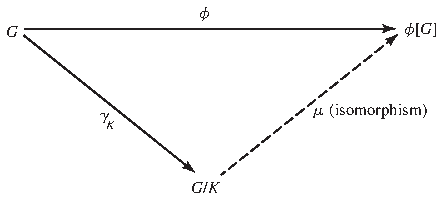
\includegraphics[width=0.604\linewidth,height=.8\textheight,keepaspectratio]{assets/p162_10.pdf}\end{center}
\begin{center}\small\textbf{16.1 Figure}\end{center}
\end{BookFloat}

\BookLabel{16.2 Theorem} \textbf{(First Isomorphism Theorem)} Let \BookInline{\phi:G\to G^{\prime }} be a homomorphism with kernel \BookInline{K,\allowbreak } and let \BookInline{\gamma _{K}:G\to G/K} be the canonical homomorphism. There is a unique isomorphism \BookInline{\mu:G/K\to \phi [G]} such that \BookInline{\phi (x)= \mu (\gamma _{K}(x))} for each \BookInline{x\in G.}\BookEnd{\blacklozenge}

The lemma that follows will be of great aid in our proof and intuitive understanding of the other two isomorphism theorems.

\BookLabel{16.3 Lemma} Let \BookInline{N} be a normal subgroup of a group \BookInline{G} and let \BookInline{\gamma:G\to G/N} be the canonical homomorphism. Then the map \BookInline{\phi } from the set of normal subgroups of \BookInline{G} containing \BookInline{N} to the set of normal subgroups of \BookInline{G/N} given by \BookInline{\phi (L)= \gamma [L]} is one-to-one and onto.

\BookLabel{\textit{Proof}} Theorem 13.18 shows that if \BookInline{L} is a normal subgroup of \BookInline{G} containing \BookInline{N,\allowbreak } then \BookInline{\phi (L)= } \BookInline{\gamma [L]} is a normal subgroup of \BookInline{G/N.} Because \BookInline{N\leq L,\allowbreak } for each \BookInline{x\in L} the entire coset \BookInline{xN} in \BookInline{G} is contained in \BookInline{L.} Thus by Theorem \BookInline{10.17,\allowbreak \gamma ^{- 1}[\phi (L)]= L.} Consequently, if \BookInline{L} and \BookInline{M} are normal subgroups of \BookInline{G,\allowbreak } both containing \BookInline{N,\allowbreak } and if \BookInline{\phi (L)= \phi (M)= H,\allowbreak } then \BookInline{L= \gamma ^{- 1}[H]= M.} Therefore \BookInline{\phi } is one-to-one.

\end{BookBody}

% Source PDF page 163; original printed page 146
\BookSource{163}{146}
\BookNarrativetrue

\begin{BookBody}

If \BookInline{H} is a normal subgroup of \BookInline{G/N,\allowbreak } then \BookInline{\gamma ^{- 1}[H]} is a normal subgroup of \BookInline{G} by Theorem 13.18. Because \BookInline{N\in H} and \BookInline{\gamma ^{- 1}[\{N\}]= N,\allowbreak } we see that \BookInline{N\subseteq \gamma ^{- 1}[H].} Then \BookInline{\phi (\gamma ^{- 1}[H])= \gamma [\gamma ^{- 1}[H]]= H.} This shows that \BookInline{\phi } is onto the set of normal subgroups of \BookInline{G/N.}\BookEnd{\blacklozenge}

If \BookInline{H} and \BookInline{N} are subgroups of a group \BookInline{G,\allowbreak } then we let

\begin{center}\begin{adjustbox}{max width=\linewidth}\BookInline{\displaystyle HN= \{hn\mid h\in H,\allowbreak n\in N\}.}\end{adjustbox}\end{center}

\noindent We define the\textbf{ join} \BookInline{H\vee N} of \BookInline{H} and \BookInline{N} as the intersection of all subgroups of \BookInline{G} that contain \BookInline{HN;} thus \BookInline{H\vee N} is the smallest subgroup of \BookInline{G} containing \BookInline{HN.} Of course \BookInline{H\vee N} is also the smallest subgroup of \BookInline{G} containing both \BookInline{H} and \BookInline{N,\allowbreak } since any such subgroup must contain \BookInline{HN.} In general\BookInline{,\allowbreak HN} need not be a subgroup of \BookInline{G.} However, we have the following lemma.

\BookLabel{16.4 Lemma} If \BookInline{N} is a normal subgroup of \BookInline{G,\allowbreak } and if \BookInline{H} is any subgroup of \BookInline{G,\allowbreak } then \BookInline{H\vee N= HN= } \BookInline{NH.} Furthermore, if \BookInline{H} is also normal in \BookInline{G,\allowbreak } then \BookInline{HN} is normal in \BookInline{G.}

\BookLabel{\textit{Proof}} We show that \BookInline{HN} is a subgroup of \BookInline{G,\allowbreak } from which \BookInline{H\vee N= HN} follows at once. Let \BookInline{h_{1},\allowbreak h_{2}\in H} and \BookInline{n_{1},\allowbreak n_{2}\in N.} Since \BookInline{N} is a normal subgroup, we have \BookInline{n_{1}h_{2}= h_{2}n_{3}} for some \BookInline{n_{3}\in N.} Then \BookInline{(h_{1}n_{1})(h_{2}n_{2})= h_{1}(n_{1}h_{2})n_{2}= h_{1}(h_{2}n_{3})n_{2}= (h_{1}h_{2})(n_{3}n_{2})\in HN,\allowbreak } so \BookInline{HN} is closed under the induced operation in \BookInline{G.} Clearly \BookInline{e= ee} is in \BookInline{HN.} For \BookInline{h\in H} and \BookInline{n\in N,\allowbreak } we have \BookInline{(hn)^{- 1}= n^{- 1}h^{- 1}= h^{- 1}n_{4}} for some \BookInline{n_{4}\in N,\allowbreak } since \BookInline{N} is a normal subgroup. Thus \BookInline{(hn)^{- 1}\in HN,\allowbreak } so \BookInline{HN\leq G.} A similar argument shows that \BookInline{NH} is a subgroup, so \BookInline{NH= H\vee N= HN.}

Now suppose that \BookInline{H} is also normal in \BookInline{G,\allowbreak } and let \BookInline{h\in H,\allowbreak n\in N,\allowbreak } and \BookInline{g\in G.} Then \BookInline{ghng^{- 1}= (ghg^{- 1})(gng^{- 1})\in HN,\allowbreak } so \BookInline{HN} is indeed normal in \BookInline{G.}\BookEnd{\blacklozenge}

We are now ready for the second isomorphism theorem.

\BookLabel{16.5 Theorem} \textbf{(Second Isomorphism Theorem)} Let \BookInline{H} be a subgroup of \BookInline{G} and let \BookInline{N} be a normal subgroup of \BookInline{G.} Then \BookInline{(HN)/N\simeq H/(H\cap N).}

\BookLabel{\textit{Proof}} Since \BookInline{N\leq HN\leq G} and \BookInline{N} is a normal subgroup of \BookInline{G,\allowbreak N} is a normal subgroup of \BookInline{HN,\allowbreak } which allows us to form the group \BookInline{HN/N.} We define a map \BookInline{\phi:H\to HN/N} by \BookInline{\phi (h)= hN.} The map \BookInline{\phi } is a homomorphism since for any \BookInline{h_{1},\allowbreak h_{2}\in H,\allowbreak }

\begin{center}\begin{adjustbox}{max width=\linewidth}\BookInline{\displaystyle \phi (h_{1}h_{2})= (h_{1}h_{2})N= (h_{1}N)(h_{2}N)= \phi (h_{1})\phi (h_{2}).}\end{adjustbox}\end{center}

\noindent The map \BookInline{\phi } maps onto \BookInline{HN/N} since any element of \BookInline{HN/N} can be written as \BookInline{hnN} for some \BookInline{h\in H} and \BookInline{n\in N} and \BookInline{hnN= hN= \phi (h).} We now compute the kernel of \BookInline{\phi.}

\begin{center}\begin{adjustbox}{max width=\linewidth}\BookInline{\displaystyle \;\text{Ker}\;(\phi )= \{h\in H\mid hN= N\}= \{h\in H\mid h\in N\}= H\cap N}\end{adjustbox}\end{center}

\noindent By the First Isomorphism Theorem, Theorem 16.2, the map \BookInline{\mu:H/(H\cap N)\to HN/N} defined by \BookInline{\mu (h(H\cap N))= hN} is an isomorphism\BookInline{.}\BookEnd{\blacklozenge}

\BookLabel{16.6 Example} Let \BookInline{G= \mathbb{Z}\times \mathbb{Z}\times \mathbb{Z},\allowbreak H= \mathbb{Z}\times \mathbb{Z}\times \{0\},\allowbreak } and \BookInline{N= \{0\}\times \mathbb{Z}\times \mathbb{Z}.} Then clearly \BookInline{HN= } \BookInline{\mathbb{Z}\times \mathbb{Z}\times \mathbb{Z}} and \BookInline{H\cap N= \{0\}\times \mathbb{Z}\times \{0\}.} We have \BookInline{(HN)/N\simeq \mathbb{Z}} and we also have \BookInline{H/(H\cap N)\simeq \mathbb{Z}.}\BookEnd{\blacktriangle}

\BookLabel{16.7 Example} Let \BookInline{G= \mathbb{Z},\allowbreak N= \langle n\rangle,\allowbreak } and \BookInline{H= \langle h\rangle } where \BookInline{n} and \BookInline{h} are positive. The group \BookInline{\mathbb{Z}} is abelian, so \BookInline{N} is a normal subgroup of \BookInline{Z.} Since \BookInline{\mathbb{Z}} is an additive group, we write \BookInline{N+ H} instead of \BookInline{NH} to avoid confusion. The group \BookInline{N+ H= \langle }gcd\BookInline{(n,\allowbreak h)\rangle } since anything in \BookInline{N+ H} is a multiple of gcd\BookInline{(n,\allowbreak h)} and gcd\BookInline{(n,\allowbreak h)= xn+ yh\in N+ H} for some integers \BookInline{x} and \BookInline{y.} Also\BookInline{,\allowbreak N\cap H= \langle }lcm\BookInline{(n,\allowbreak h)\rangle } since \BookInline{a\in N\cap H} if and only if \BookInline{a} is a multiple of both \BookInline{n} and \BookInline{h.} The Second Isomorphism Theorem states that \BookInline{(N+ H)/N= \langle }gcd\BookInline{(n,\allowbreak h)\rangle /\langle n\rangle } 
% Source PDF page 164; original printed page 147
\BookSource{164}{147}
is isomorphic with \BookInline{H/(N\cap H)= \langle h\rangle /\langle }lcm\BookInline{(n,\allowbreak h)\rangle.} In Exercise 10, you will be asked to prove that if \BookInline{a,\allowbreak b\in \mathbb{Z}^{+ }} and \BookInline{a} divides \BookInline{b,\allowbreak } then \BookInline{|\langle a\rangle /\langle b\rangle |= b/a.} Since \BookInline{\langle }gcd\BookInline{(n,\allowbreak h)\rangle /\langle n\rangle \simeq } \BookInline{\langle h\rangle /\langle }lcm\BookInline{(n,\allowbreak h)\rangle,\allowbreak } we have \BookInline{n\;\text{lcm}\;(n,\allowbreak h)}

\end{BookBody}

\BookNarrativetrue

\begin{BookBody}

\begin{center}\begin{adjustbox}{max width=\linewidth}\BookInline{\displaystyle \begin{aligned}\frac{n}{\gcd(n,\allowbreak  h)} &= \frac{\operatorname{lcm}(n,\allowbreak  h)}{h} \\nh &= \gcd(n,\allowbreak  h) \mathrm{lcm}(n,\allowbreak  h),\allowbreak \end{aligned}}\end{adjustbox}\end{center}

\noindent which provides a complicated way of proving a basic number theory fact! We conclude that

\begin{center}\begin{adjustbox}{max width=\linewidth}\BookInline{\displaystyle \langle \;\text{gcd}\;(n,\allowbreak h)\rangle /\langle n\rangle \simeq \langle h\rangle /\langle \;\text{lcm}\;(n,\allowbreak h)\rangle \simeq \mathbb{Z}_{\;\text{gcd}\;(n,\allowbreak h)}^{n}}\end{adjustbox}\end{center}

\noindent since a factor group of a cyclic group is cyclic. \BookEnd{\blacktriangle}

If \BookInline{H} and \BookInline{K} are two normal subgroups of \BookInline{G} and \BookInline{K\leq H,\allowbreak } then \BookInline{H/K} is a normal subgroup of \BookInline{G/K.} The third isomorphism theorem concerns these groups.

\BookLabel{16.8 Theorem} \textbf{(Third Isomorphism Theorem)} Let \BookInline{H} and \BookInline{K} be normal subgroups of a group \BookInline{G} with \BookInline{K\leq H.} Then \BookInline{G/H\simeq (G/K)/(H/K).}

\BookLabel{\textit{Proof}} Since \BookInline{K} is a subgroup of \BookInline{H,\allowbreak } for any \BookInline{g\in G,\allowbreak gK\subseteq gH.} That is, each left coset of \BookInline{K} is completely contained in one coset of \BookInline{H.} We define \BookInline{\phi:G/K\to G/H} by \BookInline{\phi (gK)= gH.} That is, we map a coset of \BookInline{K} to the coset of \BookInline{H} that contains it. Again, our strategy is to use the First Isomorphism Theorem. The map \BookInline{\phi } is a homomorphism since for any \BookInline{g_{1},\allowbreak g_{2}\in G,\allowbreak }

\begin{center}\begin{adjustbox}{max width=\linewidth}\BookInline{\displaystyle \begin{aligned}\phi ((g_{1}K)(g_{2}K))&= \phi ((g_{1}g_{2})K)= (g_{1}g_{2})H \\ &= (g_{1}H)(g_{2}H) \\ &= \phi (g_{1}K)\phi (g_{2}K).\end{aligned}}\end{adjustbox}\end{center}

\noindent The map \BookInline{\phi } maps onto \BookInline{G/H} since for any coset \BookInline{gH\in G/H,\allowbreak \phi (gK)= gH.} We now compute the kernel of \BookInline{\phi.}

\begin{center}\begin{adjustbox}{max width=\linewidth}\BookInline{\displaystyle \begin{aligned}\;\text{Ker}\;(\phi )&= \{gK\in G/K\mid gH= H\} \\ &= \{gK\in G/K\mid g\in H\} \\ &= H/K.\end{aligned}}\end{adjustbox}\end{center}

\noindent By the First Isomorphism Theorem \BookInline{(G/K)/(H/K)} is isomorphic with \BookInline{G/H} and a formula for an isomorphism \BookInline{\mu:(G/K)/(H/K)\to G/H} is \BookInline{\mu ((gK)H/K)= gH.}\BookEnd{\blacklozenge}

The formula for the isomorphism in the previous proof says that if we collapse the subgroup \BookInline{K} in \BookInline{G} to form \BookInline{G/K} and then collapse all the \BookInline{K} cosets inside of \BookInline{H} we have the same group as collapsing the subgroup \BookInline{H.} Figure 16.9 illustrates the situation. Think of the large ellipse as being the group \BookInline{G.} The cosets of \BookInline{H} are the sets bounded by the thick solid lines. The cosets of \BookInline{K} are the smaller sets inside the cosets of \BookInline{H.} The set \BookInline{G/H} consists of the cosets of \BookInline{H,\allowbreak } which are represented by the four larger areas, each of which is one point in \BookInline{G/H.} On the other hand\BookInline{,\allowbreak G/K} is represented by the twelve smaller sets each collapsed to a point. Then \BookInline{(G/K)/(H/K)} collapses each of the three small areas in the same \BookInline{H} coset to their common \BookInline{H} coset. Either way, we end up collapsing each \BookInline{H} coset to a point.

It is sometimes difficult to think about what groups look like when they contain more than one factor group in their definition. For example, what does an element of \BookInline{(G/K)/(H/K)} really look like? Keep in mind that a factor group has cosets of the subgroup as elements. Example 16.10 is intended to clarify what the group \BookInline{(G/K)/(H/K)} looks like and to explicitly show what the isomorphism of Theorem 16.8 looks like.

\end{BookBody}

% Source PDF page 165; original printed page 148
\BookSource{165}{148}
\BookNarrativetrue

\begin{BookBody}

\begin{BookFloat}{16_isomorphism_theorems-p165-0}
\begin{center}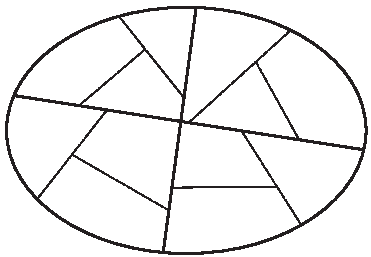
\includegraphics[width=0.509\linewidth,height=.8\textheight,keepaspectratio]{assets/p165_00.pdf}\end{center}
\begin{center}\small\textbf{16.9 Figure}\end{center}
\end{BookFloat}

\BookLabel{16.10 Example} Let \BookInline{G= \mathbb{Z}_{8},\allowbreak H= \langle 2\rangle = \{0,\allowbreak 2,\allowbreak 4,\allowbreak 6\}<G,\allowbreak } and \BookInline{K= \langle 4\rangle = \{0,\allowbreak 4\}<H.} We list the elements of each of the factor groups used in Theorem 16.8.

\begin{center}\begin{adjustbox}{max width=\linewidth}\BookInline{\displaystyle \begin{aligned}G/K&= \{\{0,\allowbreak 4\},\allowbreak \{1,\allowbreak 5\},\allowbreak \{2,\allowbreak 6\},\allowbreak \{3,\allowbreak 7\}\} \\ G/H&= \{\{0,\allowbreak 2,\allowbreak 4,\allowbreak 6\},\allowbreak \{1,\allowbreak 3,\allowbreak 5,\allowbreak 7\}\} \\ H/K&= \{\{0,\allowbreak 4\},\allowbreak \{2,\allowbreak 6\}\}\end{aligned}}\end{adjustbox}\end{center}

\noindent Before listing the elements of \BookInline{(G/K)/(H/K)} we note that any element of this group would be a coset of the subgroup \BookInline{H/K<G/K.} So each element is a set whose elements are sets.

\begin{center}\begin{adjustbox}{max width=\linewidth}\BookInline{\displaystyle (G/K)/(H/K)= \{\{\{0,\allowbreak 4\},\allowbreak \{2,\allowbreak 6\}\},\allowbreak \{\{1,\allowbreak 5\},\allowbreak \{3,\allowbreak 7\}\}\}}\end{adjustbox}\end{center}

\noindent Comparing \BookInline{G/H} and \BookInline{(G/K)/(H/K),\allowbreak } we see that each element in \BookInline{G/H} is the union of two cosets of \BookInline{K} in \BookInline{G/K.} Also, the isomorphism in Theorem 16.8 is the map \BookInline{\phi:} \BookInline{(G/K)/(H/K)\to G/H} defined by

\begin{center}\begin{adjustbox}{max width=\linewidth}\BookInline{\displaystyle \begin{aligned}\phi (\{\{0,\allowbreak 4\},\allowbreak \{2,\allowbreak 6\}\})&= \{0,\allowbreak 4,\allowbreak 2,\allowbreak 6\}\;\text{and}\; \\ \phi (\{\{1,\allowbreak 5\},\allowbreak \{3,\allowbreak 7\}\})&= \{1,\allowbreak 5,\allowbreak 3,\allowbreak 7\}.\end{aligned}}\end{adjustbox}\end{center}

\noindent So as illustrated in Figure 16.9, collapsing \BookInline{H} to form \BookInline{G/H} can be accomplished by first collapsing \BookInline{K} and then collapsing \BookInline{H/K.}\BookEnd{\blacktriangle}

\end{BookBody}

\BookNarrativefalse

\begin{BookBody}

\BookExerciseTitle{16}

\BookTextHeading{\textbf{Computations}}

\noindent In using the three isomorphism theorems, it is often necessary to know the actual correspondence given by the isomorphism and not just the fact that the groups are isomorphic. The first six exercises give us training for this.

\BookExercise{1.}{Let \BookInline{\phi:\mathbb{Z}_{12}\to \mathbb{Z}_{3}} be the homomorphism such that \BookInline{\phi (1)= 2.}}

\BookExercise{a.}{Find the kernel \BookInline{K} of \BookInline{\phi.}}

\BookExercise{b.}{List the cosets in \BookInline{\mathbb{Z}_{12}/K,\allowbreak } showing the elements in each coset.}

\BookExercise{c.}{Give the correspondence between \BookInline{\mathbb{Z}_{12}/K} and \BookInline{\mathbb{Z}_{3}} given by the map \BookInline{\mu } described in Theorem 16.2.}

\BookExercise{2.}{Let \BookInline{\phi:\mathbb{Z}_{18}\to \mathbb{Z}_{12}} be the homomorphism where \BookInline{\phi (1)= 10.}}

\BookExercise{a.}{Find the kernel \BookInline{K} of \BookInline{\phi.}}

\BookExercise{b.}{List the cosets in \BookInline{\mathbb{Z}_{18}/K,\allowbreak } showing the elements in each coset.}

\BookExercise{c.}{Find the group \BookInline{\phi [\mathbb{Z}_{18}].}}

\BookExercise{d.}{Give the correspondence between \BookInline{\mathbb{Z}_{18}/K} and \BookInline{\phi [\mathbb{Z}_{18}]} given by the map \BookInline{\mu } described in Theorem 16.2.}

\end{BookBody}

% Continuation on source PDF page 166, preceding Section 17
\BookNarrativefalse

\begin{BookBody}

\BookExercise{3.}{In the group \BookInline{\mathbb{Z}_{24},\allowbreak } let \BookInline{H= \langle 4\rangle } and \BookInline{N= \langle 6\rangle.}}

\BookExercise{a.}{List the elements in \BookInline{HN(}which we might write \BookInline{H+ N} for these additive groups) and in \BookInline{H\cap N.}}

\BookExercise{b.}{List the cosets in \BookInline{HN/N,\allowbreak } showing the elements in each coset.}

\BookExercise{c.}{List the cosets in \BookInline{H/(H\cap N),\allowbreak } showing the elements in each coset.}

\BookExercise{d.}{Give the correspondence between \BookInline{H/(H\cap N)} and \BookInline{HN/N} described in the proof of Theorem 16.5.}

\BookExercise{4.}{Repeat Exercise 3 for the dihedral group \BookInline{D_{6}} with \BookInline{N= \{\iota,\allowbreak \mu,\allowbreak \rho ^{2},\allowbreak \mu \rho ^{2},\allowbreak \rho ^{4},\allowbreak \mu \rho ^{4}\}} and \BookInline{H= \langle \rho \rangle.}}

\BookExercise{5.}{In the group \BookInline{G= \mathbb{Z}_{24},\allowbreak } let \BookInline{H= \langle 4\rangle } and \BookInline{K= \langle 8\rangle.}}

\BookExercise{a.}{List the cosets in \BookInline{G/H,\allowbreak } showing the elements in each coset.}

\BookExercise{b.}{List the cosets in \BookInline{G/K,\allowbreak } showing the elements in each coset.}

\BookExercise{c.}{List the cosets in \BookInline{H/K,\allowbreak } showing the elements in each coset.}

\BookExercise{d.}{List the cosets in \BookInline{(G/K)/(H/K),\allowbreak } showing the elements in each coset.}

\BookExercise{e.}{Give the correspondence between \BookInline{(G/K)/(H/K)} and \BookInline{G/H} described in the proof of Theorem 16.8.}

\BookExercise{6.}{Repeat Exercise 5 for the dihedral group \BookInline{G= D_{8},\allowbreak H= \langle \rho ^{2}\rangle = \{\iota,\allowbreak \rho ^{2},\allowbreak \rho ^{4},\allowbreak \rho ^{6}\},\allowbreak } and \BookInline{K= \langle \rho ^{4}\rangle = \{\iota,\allowbreak \rho ^{4}\}.}}

\BookTextHeading{\textbf{Theory}}

\BookExercise{7.}{Show directly from the definition of a normal subgroup that if \BookInline{H} and \BookInline{N} are subgroups of a group \BookInline{G,\allowbreak } and \BookInline{N} is normal in \BookInline{G,\allowbreak } then \BookInline{H\cap N} is normal in \BookInline{H.}}

\BookExercise{8.}{Let \BookInline{H,\allowbreak K,\allowbreak } and \BookInline{L} be normal subgroups of \BookInline{G} with \BookInline{H<K<L.} Let \BookInline{A= G/H,\allowbreak B= K/H,\allowbreak } and \BookInline{C= L/H.}}

\BookExercise{a.}{Show that \BookInline{B} and \BookInline{C} are normal subgroups of \BookInline{A,\allowbreak } and \BookInline{B<C.}}

\BookExercise{b.}{To what factor group of \BookInline{G} is \BookInline{(A/B)/(C/B)} isomorphic?}

\BookExercise{9.}{Let \BookInline{K} and \BookInline{L} be normal subgroups of \BookInline{G} with \BookInline{K\vee L= G,\allowbreak } and \BookInline{K\cap L= \{e\}.} Show that \BookInline{G/K\simeq L} and \BookInline{G/L\simeq K.}}

\BookExercise{10.}{Use one of the Isomorphism Theorems to prove that if \BookInline{a,\allowbreak b\in \mathbb{Z}^{+ }} and \BookInline{a} divides \BookInline{b,\allowbreak } then \BookInline{|a\mathbb{Z}/b\mathbb{Z}|= b/a.}}

\BookExercise{11.}{Let \BookInline{G} be a group with subgroups \BookInline{H^{\ast }\leq H\leq G} and \BookInline{K^{\ast }\leq K\leq G.} Prove that the sets \BookInline{H^{\ast }(H\cap K^{\ast })\cap (H\cap K)} and \BookInline{(H^{\ast }\cap K)(H\cap K^{\ast })} are equal.}

\end{BookBody}
\ifdefined\BookMaster\let\BookFinish\relax\else\def\BookFinish{\end{document}}\fi\BookFinish

\clearpage
% !TeX program = xelatex
\ifdefined\BookMaster\else
\documentclass[11pt,oneside]{article}
% !TeX program = xelatex
\usepackage[b5paper,left=22mm,right=22mm,top=20mm,bottom=22mm,footskip=11mm]{geometry}
\usepackage{fontspec}
\setmainfont{TeX Gyre Termes}
\setsansfont{TeX Gyre Heros}
\usepackage{amsmath,amssymb,mathtools,amsthm}
\renewcommand{\cdots}{\mathinner{\cdotp\cdotp\cdotp}}
\usepackage{graphicx,adjustbox,array,booktabs,longtable,multirow,enumitem,changepage,needspace}
\usepackage[table]{xcolor}
\usepackage{fancyhdr}
\raggedbottom
\interfootnotelinepenalty=10000
\newcommand{\BookFootnote}[2]{\begingroup\renewcommand{\thefootnote}{\fnsymbol{footnote}}\footnote[#1]{#2}\endgroup}
\newcommand{\BookFootnoteMark}[1]{\begingroup\renewcommand{\thefootnote}{\fnsymbol{footnote}}\footnotemark[#1]\endgroup}
\newcommand{\BookFootnoteText}[2]{\begingroup\renewcommand{\thefootnote}{\fnsymbol{footnote}}\footnotetext[#1]{#2}\endgroup}
\newenvironment{BookFloat}[1]{\par\addvspace{.6\baselineskip}\noindent\def\BookFloatID{#1}\begin{minipage}{\linewidth}\phantomsection\label{bookfloat:#1:start}}{\phantomsection\label{bookfloat:\BookFloatID:end}\end{minipage}\par\addvspace{.6\baselineskip}}

\usepackage[unicode,hidelinks]{hyperref}
\pagestyle{fancy}
\fancyhf{}
\newcommand{\BookFooter}{}
\fancyfoot[L]{\parbox[b]{\dimexpr\textwidth-15mm}{\footnotesize\BookFooter}}
\fancyfoot[R]{\footnotesize\thepage}
\renewcommand{\headrulewidth}{0pt}
\renewcommand{\footrulewidth}{0pt}
\setlength{\parindent}{0pt}
\setlength{\parskip}{0.2em}
\setlength{\emergencystretch}{3em}
\setlist{nosep,leftmargin=1.7em,labelsep=.65em}
\newif\ifBookNarrative
\BookNarrativetrue
\newenvironment{BookBody}{\setlength{\parindent}{0pt}}{}
\newcommand{\BookStatement}[1]{\par\addvspace{.6\baselineskip}\noindent #1\enspace\ignorespaces}
\newcommand{\BookLabel}[1]{\par\addvspace{.6\baselineskip}\needspace{3\baselineskip}\noindent\textbf{#1}\quad\ignorespaces}
\newcommand{\BookHeading}[1]{\par\addvspace{\baselineskip}\needspace{4\baselineskip}\noindent{\large\bfseries #1}\par\medskip}
\newcommand{\BookSubheading}[1]{\par\addvspace{.7\baselineskip}\needspace{3\baselineskip}\noindent{\bfseries #1}\par\smallskip}
\newcommand{\BookTextHeading}[1]{\par\addvspace{.7\baselineskip}\needspace{3\baselineskip}\noindent #1\par\smallskip}
\newcommand{\BookSectionTitle}[2]{\par\addvspace{1.2\baselineskip}\needspace{5\baselineskip}\noindent\colorbox{gray!25}{\sffamily\bfseries\small SECTION #1}\quad{\large\bfseries #2}\par\medskip}
\newcommand{\BookExerciseTitle}[1]{\par\addvspace{\baselineskip}\needspace{4\baselineskip}\noindent{\color{gray}\rule{1.5mm}{1.5mm}}\enspace{\large\bfseries Exercises #1}\par\medskip}
\newcommand{\BookBullet}[1]{\begin{list}{\textbullet}{\setlength{\leftmargin}{1.7em}\setlength{\labelwidth}{1em}\setlength{\labelsep}{.7em}\setlength{\topsep}{0pt}\setlength{\parsep}{0pt}\setlength{\itemsep}{0pt}}\item #1\end{list}}
\newcommand{\BookExercise}[2]{\begin{list}{\textbf{#1}}{\setlength{\leftmargin}{2.2em}\setlength{\labelwidth}{1.5em}\setlength{\labelsep}{.7em}\setlength{\topsep}{.15em}\setlength{\parsep}{0pt}\setlength{\itemsep}{0pt}}\item #2\end{list}}
\newcommand{\BookEnd}[1]{\unskip\nobreak\hfill\ensuremath{#1}}
\newcommand{\BookSource}[2]{\phantomsection\label{sourcepage:#1}} % Source-page anchors, retained through reflow.
\usepackage{multicol}
\usepackage{tikz}
\newcommand{\BookPartEntry}[2]{\par\noindent\makebox[17mm][l]{\bfseries Section #1}#2\par}
\newcommand{\BookPartTitle}[3]{\par\bigskip\noindent\begin{tikzpicture}\node[anchor=north west,inner sep=0pt,outer sep=0pt] (bookpart) at (0,0) {\begin{minipage}{\dimexpr\linewidth-.5pt}\hspace*{26mm}\begin{minipage}[t]{\dimexpr\linewidth-26mm}\begin{adjustbox}{max width=\linewidth}{\fontsize{20}{24}\selectfont\bfseries #2}\end{adjustbox}\par\vspace{6mm}\hrule\vspace{6mm}{\sffamily\footnotesize\setlength{\parskip}{.3em}#3}\vspace{3mm}\end{minipage}\end{minipage}};\path[shade,top color=gray!60,bottom color=white] (0,0) rectangle ([xshift=24mm]bookpart.south west);\node[anchor=north,font=\sffamily\bfseries\small] at (12mm,-2mm) {PART};\node[anchor=north,font=\sffamily\bfseries\Huge] at (12mm,-7mm) {#1};\end{tikzpicture}\par\bigskip}
\newsavebox{\BookMathBox}
\makeatletter
\newcommand{\BookInline}[1]{\leavevmode\hskip0pt\relax\begingroup\in@{\begin}{#1}\ifin@\sbox{\BookMathBox}{\(#1\)}\ifdim\wd\BookMathBox>\dimexpr\linewidth-1em\relax\resizebox{\dimexpr\linewidth-1em\relax}{!}{\usebox{\BookMathBox}}\else\(#1\)\fi\else\in@{\left}{#1}\ifin@\sbox{\BookMathBox}{\(#1\)}\ifdim\wd\BookMathBox>\dimexpr\linewidth-1em\relax\resizebox{\dimexpr\linewidth-1em\relax}{!}{\usebox{\BookMathBox}}\else\(#1\)\fi\else\(#1\)\fi\fi\endgroup\hskip0pt\relax}
\makeatother
\DeclareMathOperator{\Aut}{Aut}
\DeclareMathOperator{\End}{End}
\DeclareMathOperator{\Hom}{Hom}
\DeclareMathOperator{\GF}{GF}
\DeclareMathOperator{\irr}{irr}
\DeclareMathOperator{\lt}{lt}
\DeclareMathOperator{\lp}{lp}
\providecommand{\textcircled}[1]{\textnormal{(#1)}}

\begin{document}
\fi
\renewcommand{\BookFooter}{Section 17 Sylow Theorems}
\pdfbookmark[0]{Section 17 Sylow Theorems}{17_sylow_theorems}
\ifdefined\BookMaster\else\setcounter{page}{149}\fi
% Source PDF page 166; original printed page 149
\BookSource{166}{149}
\BookNarrativetrue

\begin{BookBody}

\BookSectionTitle{17}{Sylow Theorems}

\noindent The Fundamental Theorem for Finitely Generated Abelian Groups (Theorems 9.12 and 9.14) give us complete information about all finite abelian groups. The study of finite nonabelian groups is much more complicated. The Sylow theorems give us some important information about them.

The Theorem of Lagrange says that if \BookInline{H} is a subgroup of a finite group \BookInline{G,\allowbreak } then the order of \BookInline{H} divides the order of \BookInline{G.} The Fundamental Theorem for Finitely Generated Abelian Groups implies that if \BookInline{k} divides the order of a finite abelian group \BookInline{G,\allowbreak } then \BookInline{G} has a subgroup of order \BookInline{k.} The situation is different for nonabelian groups. Example 13.6 shows that although \BookInline{A_{4}} has 12 elements, it has no subgroup of order 6. Furthermore, for \BookInline{n\geq 5,\allowbreak A_{n}} can have no subgroup of index 2 since \BookInline{A_{n}} is simple and any subgroup of index 2 is a normal subgroup. On the positive side, Cauchy’s theorem (14.20) says that if the prime number \BookInline{p} divides the order of a group \BookInline{G,\allowbreak } then \BookInline{G} has a subgroup of order \BookInline{p.} The Sylow theorems generalize Cauchy’s theorem to show that if \BookInline{p^{n}} divides the order of \BookInline{G,\allowbreak } then \BookInline{G} has a subgroup of order \BookInline{p^{n}} as long as \BookInline{p} is a prime number. Furthermore, Sylow’s theorems gives us information about relationships between these subgroups of \BookInline{G.} As we shall see, this information is very useful in the study of finite nonabelian groups.

Proofs of the Sylow theorems give us another application of action of a group on a set described in Section 14. This time, the set itself is formed from the group; in some instances the set is the group itself, sometimes it is a collection of cosets of a subgroup, and sometimes it is a collection of subgroups.

\end{BookBody}

% Source PDF page 167; original printed page 150
\BookSource{167}{150}
\BookNarrativetrue

\begin{BookBody}

\BookTextHeading{\textbf{The Sylow Theorems}  }

\noindent Let \BookInline{G} be a group, and let \BookInline{\mathcal{S}} be the collection of all subgroups of \BookInline{G.} We make \BookInline{\mathcal{S}} into a \BookInline{G-}set by letting \BookInline{G} act on \BookInline{\mathcal{S}} by conjugation. That is, if \BookInline{H\in \mathcal{S}} so \BookInline{H\leq G} and \BookInline{g\in G,\allowbreak } then \BookInline{g} acting on \BookInline{H} yields the conjugate subgroup \BookInline{gHg^{- 1}.(}To avoid confusion, we will never write this action as \BookInline{gH.)} By Theorem \BookInline{14.13G_{H}= \{g\in G\mid gHg^{- 1}= H\}} is a subgroup of \BookInline{G,\allowbreak } which is called an isotropy subgroup. In Exercise 14 you will be asked to show directly that \BookInline{G_{H}} is a subgroup of \BookInline{G.} Since \BookInline{G_{H}} consists of\textit{ all} elements of \BookInline{G} that leave \BookInline{H} invariant under conjugation\BookInline{,\allowbreak G_{H}} is the largest subgroup of \BookInline{G} having \BookInline{H} as a normal subgroup.

\BookLabel{17.1 Definition} The subgroup \BookInline{G_{H}} just discussed is the\textbf{ normalizer of} \BookInline{H} \textbf{in} \BookInline{G} and will be denoted \BookInline{N[H]} from now on\BookInline{.}\BookEnd{\blacksquare}

In the proof of the lemma that follows, we will use the fact that if \BookInline{H} is a\textit{ finite} subgroup of a group \BookInline{G,\allowbreak } then \BookInline{g\in N[H]} if \BookInline{ghg^{- 1}\in H} for all \BookInline{h\in H.} To see this, note that if \BookInline{gh_{1}g^{- 1}= gh_{2}g^{- 1},\allowbreak } then \BookInline{h_{1}= h_{2}} by cancellation in the group \BookInline{G.} Thus the conjugation map \BookInline{i_{g}:H\to H} given by \BookInline{i_{g}(h)= ghg^{- 1}} is one-to-one. Because \BookInline{|H|} is finite\BookInline{,\allowbreak i_{g}} must then map \BookInline{H} \textit{onto} \BookInline{H,\allowbreak } so \BookInline{gHg^{- 1}= H} and \BookInline{g\in N[H].}

\BookLabel{17.2 Lemma} Let \BookInline{H} be a \BookInline{p-}subgroup of a finite group \BookInline{G.} Then

\begin{center}\begin{adjustbox}{max width=\linewidth}\BookInline{\displaystyle (N[H]:H)\equiv (G:H)(\;\text{mod}\;p).}\end{adjustbox}\end{center}

\BookLabel{\textit{Proof}} Let \BookInline{\mathcal{L}} be the set of left cosets of \BookInline{H} in \BookInline{G,\allowbreak } and let \BookInline{H} act on \BookInline{\mathcal{L}} by left translation, so that \BookInline{h(xH)= (hx)H.} Then \BookInline{\mathcal{L}} becomes an \BookInline{H-}set. Note that \BookInline{|\mathcal{L}|= (G:H).}

\begin{center}\begin{adjustbox}{max width=\linewidth}\BookInline{\displaystyle \mathcal{L}_{H},\allowbreak }\end{adjustbox}\end{center}

Let us determine that is, those left cosets that are fixed under action by all el-

\begin{center}\begin{adjustbox}{max width=\linewidth}\BookInline{\displaystyle xH= h(xH)}\end{adjustbox}\end{center}

\begin{center}\begin{adjustbox}{max width=\linewidth}\BookInline{\displaystyle H= x^{- 1}hxH,\allowbreak }\end{adjustbox}\end{center}

\begin{center}\begin{adjustbox}{max width=\linewidth}\BookInline{\displaystyle x^{- 1}hx\in H.}\end{adjustbox}\end{center}

\noindent ements of \BookInline{H.} Now if and only if or if and only if

\begin{center}\begin{adjustbox}{max width=\linewidth}\BookInline{\displaystyle xH= h(xH)}\end{adjustbox}\end{center}

\begin{center}\begin{adjustbox}{max width=\linewidth}\BookInline{\displaystyle h\in H}\end{adjustbox}\end{center}

\begin{center}\begin{adjustbox}{max width=\linewidth}\BookInline{\displaystyle \mathrm{f}x^{- 1}hx= x^{- 1}h(x^{- 1})^{- 1}\in H}\end{adjustbox}\end{center}

\begin{center}\begin{adjustbox}{max width=\linewidth}\BookInline{\displaystyle h\in H,\allowbreak }\end{adjustbox}\end{center}

\noindent Thus for all if and only i for all

\begin{center}\begin{adjustbox}{max width=\linewidth}\BookInline{\displaystyle x^{- 1}\in N[H]}\end{adjustbox}\end{center}

\noindent or if and only if (see the comment before the lemma), or if and only if

\begin{center}\begin{adjustbox}{max width=\linewidth}\BookInline{\displaystyle x\in N[H].}\end{adjustbox}\end{center}

\begin{center}\begin{adjustbox}{max width=\linewidth}\BookInline{\displaystyle \mathcal{L}_{H}}\end{adjustbox}\end{center}

\begin{center}\begin{adjustbox}{max width=\linewidth}\BookInline{\displaystyle N[H]}\end{adjustbox}\end{center}

Thus the left cosets in are those contained in. The number of such

\begin{center}\begin{adjustbox}{max width=\linewidth}\BookInline{\displaystyle (N[H]:H),\allowbreak \;\text{so}\;|\mathcal{L}_{H}|= (N[H]:H).}\end{adjustbox}\end{center}

\noindent cosets is

Since \BookInline{H} is a \BookInline{p-}group, it has order a power of \BookInline{p.} Theorem 14.9 then tells us that \BookInline{|\mathcal{L}|\equiv |\mathcal{L}_{H}|(}mod \BookInline{p),\allowbreak } that is, that \BookInline{(G:H)\equiv (N[H]:H)(}mod \BookInline{p).}\BookEnd{\blacklozenge}

\BookLabel{17.3 Corollary} Let \BookInline{H} be a \BookInline{p-}subgroup of a finite group \BookInline{G.} If \BookInline{p} divides \BookInline{(G:H),\allowbreak } then \BookInline{N[H]\neq H.}

\BookLabel{\textit{Proof}} It follows from Lemma 17.2 that \BookInline{p} divides \BookInline{(N[H]:H),\allowbreak } which must then be different from 1. Thus \BookInline{H\neq N[H].}\BookEnd{\blacklozenge}

\BookTextHeading{\ensuremath{\blacksquare} \textbf{HISTORICAL NOTE}  }

\noindent The Sylow theorems are due to the Norwegian mathematician Peter Ludvig Mejdell Sylow (1832–1918), who published them in a brief paper in 1872. Sylow stated the theorems in terms of permutation groups (since the abstract definition of a group had not yet been given). Georg Frobenius re-proved the theorems for abstract groups in 1887, even though he noted that in fact every group can be considered as a permutation group (Cayley’s theorem [Theorem 8.11]). Sylow himself immediately applied the theorems to the question of solving algebraic equations and showed that any equation whose Galois group has order a power of a prime \BookInline{p} is solvable by radicals.

Sylow spent most of his professional life as a high school teacher in Halden, Norway, and was only appointed to a position at Christiana University in 1898. He devoted eight years of his life to the project of editing the mathematical works of his countryman Niels Henrik Abel.

\end{BookBody}

% Source PDF page 168; original printed page 151
\BookSource{168}{151}
\BookNarrativetrue

\begin{BookBody}

\noindent We are now ready for the first of the Sylow theorems, which asserts the existence of prime-power subgroups of \BookInline{G} for any prime power dividing \BookInline{|G|.}

\BookLabel{17.4 Theorem} \textbf{(First Sylow Theorem)} Let \BookInline{G} be a finite group and let \BookInline{|G|= p^{n}m} where \BookInline{n\geq 1} and where \BookInline{p} does not divide \BookInline{m.} Then

\BookExercise{1.}{\BookInline{G} contains a subgroup of order \BookInline{p^{i}} for each \BookInline{i} where \BookInline{1\leq i\leq n,\allowbreak }}

\BookExercise{2.}{Every subgroup \BookInline{H} of \BookInline{G} of order \BookInline{p^{i}} is a normal subgroup of a subgroup of order \BookInline{p^{i+ 1}} for \BookInline{1\leq i<n.}}

\BookLabel{\textit{Proof}} (Theorem 14.20). We use an induction argument and show that the existence of a subgroup of order \BookInline{p^{i}} for \BookInline{i<n} implies the existence of a subgroup of order \BookInline{p^{i+ 1}.} Let \BookInline{H} be a subgroup of order \BookInline{p^{i}.} Since \BookInline{i<n,\allowbreak } we see \BookInline{p} divides \BookInline{(G:H).} By Lemma 17.2, we then know \BookInline{p} divides \BookInline{(N[H]:H).} Since \BookInline{H} is a normal subgroup of \BookInline{N[H],\allowbreak } we can form \BookInline{N[H]/H,\allowbreak } and we see that \BookInline{p} divides \BookInline{|N[H]/H|.} By Cauchy’s theorem, the factor group \BookInline{N[H]/H} has a subgroup \BookInline{K,\allowbreak } which is of order \BookInline{p.} If \BookInline{\gamma:N[H]\to N[H]/H} is the canonical homomorphism, then \BookInline{\gamma ^{- 1}[K]= \{x\in N[H]\mid \gamma (x)\in K\}} is a subgroup of \BookInline{N[H]} and hence of \BookInline{G.} This subgroup contains \BookInline{H} and is of order \BookInline{p^{i+ 1}.}

\BookExercise{1.}{We know \BookInline{G} contains a subgroup of order \BookInline{p} by Cauchy’s theorem}

\BookExercise{2.}{We repeat the construction in part 1 and note that \BookInline{H<\gamma ^{- 1}[K]\leq N[H]} where \BookInline{|\gamma ^{- 1}[K]|= p^{i+ 1}.} Since \BookInline{H} is normal in \BookInline{N[H],\allowbreak } it is of course normal in the possibly smaller group \BookInline{\gamma ^{- 1}[K].}\BookEnd{\blacklozenge}}

\BookLabel{17.5 Definition} A\textbf{ Sylow} \BookInline{p-}\textbf{subgroup} \BookInline{P} of a group \BookInline{G} is a maximal \BookInline{p-}subgroup of \BookInline{G,\allowbreak } that is, a \BookInline{p-}subgroup contained in no larger \BookInline{p-}subgroup\BookInline{.}\BookEnd{\blacksquare}

\noindent Let \BookInline{G} be a finite group, where \BookInline{|G|= p^{n}m} as in Theorem 17.4. The theorem shows that the Sylow \BookInline{p-}subgroups of \BookInline{G} are precisely those subgroups of order \BookInline{p^{n}.} If \BookInline{P} is a Sylow \BookInline{p-}subgroup, every conjugate \BookInline{gPg^{- 1}} of \BookInline{P} is also a Sylow \BookInline{p-}subgroup. The second Sylow theorem states that every Sylow \BookInline{p-}subgroup can be obtained from \BookInline{P} in this fashion; that is, any two Sylow \BookInline{p-}subgroups are conjugate.

\BookLabel{17.6 Theorem} \textbf{(Second Sylow Theorem)} Let \BookInline{P_{1}} and \BookInline{P_{2}} be Sylow \BookInline{p-}subgroups of a finite group \BookInline{G.} Then \BookInline{P_{1}} and \BookInline{P_{2}} are conjugate subgroups of \BookInline{G.}

\BookLabel{\textit{Proof}} Here we will let one of the subgroups act on left cosets of the other, and use Theorem 14.19. Let \BookInline{\mathcal{L}} be the collection of left cosets of \BookInline{P_{1},\allowbreak } and let \BookInline{P_{2}} act on \BookInline{\mathcal{L}} by \BookInline{y(xP_{1})= (yx)P_{1}} for \BookInline{y\in P_{2}.} Then \BookInline{\mathcal{L}} is a \BookInline{P_{2}-}set. By Theorem 14.19, \BookInline{|\mathcal{L}_{P_{2}}|\equiv |\mathcal{L}|} (mod \BookInline{p),\allowbreak } and \BookInline{|\mathcal{L}|= (G:P_{1})} is not divisible by \BookInline{p,\allowbreak \;\text{so}\;|\mathcal{L}_{P_{2}}|\neq 0.\;\text{Let}\;xP_{1}\in \mathcal{L}_{P_{2}}}. Then \BookInline{yxP_{1}= xP_{1}} for all \BookInline{y\in P_{2},\allowbreak } so \BookInline{x^{- 1}yxP_{1}= P_{1}} for all \BookInline{y\in P_{2}.} Thus \BookInline{x^{- 1}yx\in P_{1}} for all \BookInline{y\in P_{2},\allowbreak } so \BookInline{x^{- 1}P_{2}x\leq P_{1}.} Since \BookInline{|P_{1}|= |P_{2}|,\allowbreak } we must have \BookInline{P_{1}= x^{- 1}P_{2}x,\allowbreak } so \BookInline{P_{1}} and \BookInline{P_{2}} are indeed conjugate subgroups\BookInline{.}\BookEnd{\blacklozenge}

\noindent The final Sylow theorem gives information on the number of Sylow \BookInline{p-}subgroups.

\BookLabel{17.7 Theorem} \textbf{(Third Sylow Theorem)} If \BookInline{G} is a finite group and \BookInline{p} divides \BookInline{|G|,\allowbreak } then the number of Sylow \BookInline{p-}subgroups is congruent to 1 modulo \BookInline{p} and divides \BookInline{|G|.}

\BookLabel{\textit{Proof}} Let \BookInline{P} be one Sylow \BookInline{p-}subgroup of \BookInline{G.} Let \BookInline{\mathcal{S}} be the set of all Sylow \BookInline{p-}subgroups and let \BookInline{P} act on \BookInline{\mathcal{S}} by conjugation, so that \BookInline{x\in P} carries \BookInline{T\in \mathcal{S}} into \BookInline{xTx^{- 1}.} By Theorem 14.19, \BookInline{|\mathcal{S}|\equiv |\mathcal{S}_{P}|(}mod \BookInline{p).} Let us find \BookInline{\mathcal{S}_{P}.} If \BookInline{T\in \mathcal{S}_{P},\allowbreak } then \BookInline{xTx^{- 1}= T} for all \BookInline{x\in P.} Thus \BookInline{P\leq N[T].} Of course\BookInline{,\allowbreak T\leq N[T]} also. Since \BookInline{P} and \BookInline{T} are both Sylow \BookInline{p-}subgroups of \BookInline{G,\allowbreak } 
% Source PDF page 169; original printed page 152
\BookSource{169}{152}
they are also Sylow \BookInline{p-}subgroups of \BookInline{N[T].} But then they are conjugate in \BookInline{N[T]} by Theorem 17.6. Since \BookInline{T} is a normal subgroup of \BookInline{N[T],\allowbreak } it is its only conjugate in \BookInline{N[T].} Thus \BookInline{T= P.} Then \BookInline{\mathcal{S}_{P}= \{P\}.} Since \BookInline{|\mathcal{S}|\equiv |\mathcal{S}_{P}|= 1(}mod \BookInline{p),\allowbreak } we see the number of Sylow \BookInline{p-}subgroups is congruent to 1 modulo \BookInline{p.}

\end{BookBody}

\BookNarrativetrue

\begin{BookBody}

Now let \BookInline{G} act on \BookInline{\mathcal{S}} by conjugation. Since all Sylow \BookInline{p-}subgroups are conjugate, there is only one orbit in \BookInline{\mathcal{S}} under \BookInline{G.} If \BookInline{P\in \mathcal{S},\allowbreak } then \BookInline{|\mathcal{S}|= |}orbit of \BookInline{P|= (G:G_{P})} by Theorem \BookInline{14.17.(G_{P}} is, in fact, the normalizer of \BookInline{P.)} But \BookInline{(G:G_{P})} is a divisor of \BookInline{|G|,\allowbreak } so the number of Sylow \BookInline{p-}subgroups divides \BookInline{|G|.}\BookEnd{\blacklozenge}

Theorem 17.7 is really a bit better than it sounds. Let \BookInline{|G|= p^{n}m} where the prime number \BookInline{p} does not divide \BookInline{m} and suppose that \BookInline{G} contains \BookInline{k} Sylow \BookInline{p-}subgroups. Then Theorem 17.7 says that \BookInline{k} is equivalent to 1 modulo \BookInline{p} and \BookInline{k} divides \BookInline{|G|.} Since gcd\BookInline{(k,\allowbreak p)= 1,\allowbreak k} must divide \BookInline{m.}

\BookTextHeading{\textbf{Applications of the Sylow Theorems}  }

\BookLabel{17.8 Example} The Sylow 2-subgroups of \BookInline{D_{3}} have order 2. Three Sylow 2-subgroups are

\begin{center}\begin{adjustbox}{max width=\linewidth}\BookInline{\displaystyle \{\iota ,\allowbreak \mu \},\allowbreak \{\iota ,\allowbreak \mu \rho \},\allowbreak \{\iota ,\allowbreak \mu \rho ^{2}\}}\end{adjustbox}\end{center}

\noindent Notice that Theorem 17.7 says that the number \BookInline{k} of Sylow 2-subgroups must be odd and \BookInline{k} must divide 6. However, by the observation above\BookInline{,\allowbreak k} must divide 3. So in fact, the three subgroups listed are all three of the subgroups of \BookInline{D_{3}} having order \BookInline{2.}\BookEnd{\blacktriangle}

\BookLabel{17.9 Lemma} Let \BookInline{G} be a group containing normal subgroups \BookInline{H} and \BookInline{K} such that \BookInline{H\cap K= \{e\}} and \BookInline{H\vee K= G.} Then \BookInline{G} is isomorphic to \BookInline{H\times K.}\BookEnd{\blacklozenge}

\BookLabel{\textit{Proof}} We start by showing that \BookInline{hk= kh} for \BookInline{k\in K} and \BookInline{h\in H.} Consider the commutator \BookInline{hkh^{- 1}k^{- 1}= (hkh^{- 1})k^{- 1}= h(kh^{- 1}k^{- 1}).} Since \BookInline{H} and \BookInline{K} are normal subgroups of \BookInline{G,\allowbreak } the two groupings with parentheses show that \BookInline{hkh^{- 1}k^{- 1}} is in both \BookInline{K} and \BookInline{H.} Since \BookInline{K\cap H= \{e\},\allowbreak } we see that \BookInline{hkh^{- 1}k^{- 1}= e,\allowbreak } so \BookInline{hk= kh.}

Let \BookInline{\phi:H\times K\to G} be defined by \BookInline{\phi (h,\allowbreak k)= hk.} Then

\begin{center}\begin{adjustbox}{max width=\linewidth}\BookInline{\displaystyle \begin{aligned}\phi ((h,\allowbreak k)(h^{\prime },\allowbreak k^{\prime }))&= \phi (hh^{\prime },\allowbreak kk^{\prime })= hh^{\prime }kk^{\prime } \\ &= hkh^{\prime }k^{\prime }= \phi (h,\allowbreak k)\phi (h^{\prime },\allowbreak k^{\prime }),\allowbreak \end{aligned}}\end{adjustbox}\end{center}

\noindent so \BookInline{\phi } is a homomorphism.

If \BookInline{\phi (h,\allowbreak k)= e,\allowbreak } then \BookInline{hk= e,\allowbreak } so \BookInline{h= k^{- 1},\allowbreak } and both \BookInline{h} and \BookInline{k} are in \BookInline{H\cap K.} Thus \BookInline{h= } \BookInline{k= e,\allowbreak } so Ker\BookInline{(\phi )= \{(e,\allowbreak e)\}} and \BookInline{\phi } is one-to-one.

By Lemma 16.4, we know that \BookInline{HK= H\vee K,\allowbreak } and \BookInline{H\vee K= G} by hypothesis. Thus \BookInline{\phi } is onto \BookInline{G,\allowbreak } and \BookInline{H\times K\simeq G.}\BookEnd{\blacklozenge}

\noindent We turn now to a discussion of whether there exist simple groups of certain orders. We have seen that every group of prime order is simple. We also asserted that \BookInline{A_{n}} is simple for \BookInline{n\geq 5} and that \BookInline{A_{5}} is the smallest simple group that is not of prime order. There was a famous conjecture of Burnside that every finite simple group of nonprime order must be of even order. It was a triumph when this was proved by Thompson and Feit [21].

\BookLabel{17.10 Theorem} If \BookInline{p} and \BookInline{q} are distinct primes with \BookInline{p<q,\allowbreak } then every group \BookInline{G} of order \BookInline{pq} has a single subgroup of order \BookInline{q} and this subgroup is normal in \BookInline{G.} Hence \BookInline{G} is not simple. If \BookInline{q} is not congruent to 1 modulo \BookInline{p,\allowbreak } then \BookInline{G} is abelian and cyclic.

\BookLabel{\textit{Proof}} Theorems 17.4 and 17.7 tell us that \BookInline{G} has a Sylow \BookInline{q-}subgroup and that the number of such subgroups is congruent to 1 modulo \BookInline{q} and divides \BookInline{pq,\allowbreak } and therefore must divide \BookInline{p.} Since \BookInline{p<q,\allowbreak } the only possibility is the number 1. Thus there is only one Sylow

\end{BookBody}

% Source PDF page 170; original printed page 153
\BookSource{170}{153}
\BookNarrativetrue

\begin{BookBody}

\noindent \BookInline{q-}subgroup \BookInline{Q} of \BookInline{G.} This group \BookInline{Q} must be normal in \BookInline{G,\allowbreak } for under an inner automorphism it would be carried into a group of the same order, hence itself. Thus \BookInline{G} is not simple.

Likewise, there is a Sylow \BookInline{p-}subgroup \BookInline{P} of \BookInline{G,\allowbreak } and the number of these divides \BookInline{pq} and is congruent to 1 modulo \BookInline{p.} This number must be either 1 or \BookInline{q.} If \BookInline{q} is not congruent to 1 modulo \BookInline{p,\allowbreak } then the number must be 1 and \BookInline{P} is normal in \BookInline{G.} Let us assume that \BookInline{q\not \equiv 1(}mod \BookInline{p).} Since every element in \BookInline{Q} other than \BookInline{e} is of order \BookInline{q} and every element in \BookInline{P} other than \BookInline{e} is of order \BookInline{p,\allowbreak } we have \BookInline{Q\cap P= \{e\}.} Also \BookInline{Q\vee P} must be a subgroup of \BookInline{G} properly containing \BookInline{Q} and of order dividing \BookInline{pq.} Hence \BookInline{Q\vee P= G} and by Lemma 17.9 is isomorphic to \BookInline{Q\times P} or \BookInline{\mathbb{Z}_{q}\times \mathbb{Z}_{p}.} Thus \BookInline{G} is abelian and cyclic\BookInline{.}\BookEnd{\blacklozenge}

\BookLabel{17.11 Example} Recall that if \BookInline{p} is a prime number, then up to isomorphism there is only one group of order \BookInline{p} and it is cyclic. Theorem 17.10 shows that there are many nonprime numbers \BookInline{n} such that every group of order \BookInline{n} is cyclic. Since 5 is not equivalent to 1 modulo 3, by Theorem 17.10, every group of order 15 is cyclic. Exercise 33 shows that 15 is the smallest composite number with this property\BookInline{.}\BookEnd{\blacktriangle}

We need another lemma for some of the counting arguments that follow.

\BookLabel{17.12 Lemma} If \BookInline{H} and \BookInline{K} are finite subgroups of a group \BookInline{G,\allowbreak } then

\begin{center}\begin{adjustbox}{max width=\linewidth}\BookInline{\displaystyle | { \it H K } | = \frac { ( | { \cal H } | ) ( | { \cal K } | ) } { | { \cal H } \cap { \cal K } | } .}\end{adjustbox}\end{center}

\BookLabel{\textit{Proof}} Let

\begin{center}\begin{adjustbox}{max width=\linewidth}\BookInline{\displaystyle h_{1}(H\cap K),\allowbreak h_{2}(H\cap K),\allowbreak h_{3}(H\cap K),\allowbreak ...,\allowbreak h_{r}(H\cap K)}\end{adjustbox}\end{center}

\noindent be the left cosets of \BookInline{H\cap K} in \BookInline{H} with each coset listed exactly once. We let

\begin{center}\begin{adjustbox}{max width=\linewidth}\BookInline{\displaystyle S= \{h_{1},\allowbreak h_{2},\allowbreak h_{3},\allowbreak ...,\allowbreak h_{r}\},\allowbreak }\end{adjustbox}\end{center}

\noindent which includes exactly one element from each left coset of \BookInline{H\cap K} in \BookInline{H.} So

\begin{center}\begin{adjustbox}{max width=\linewidth}\BookInline{\displaystyle | S | = { \frac { | H | } { | H \cap K | } } .}\end{adjustbox}\end{center}

\noindent Let \BookInline{f:S\times K\to HK} be defined by \BookInline{f(h_{i},\allowbreak k)= h_{i}k.} We show that \BookInline{f} is one-to-one and onto.

Suppose that \BookInline{hk\in HK.} Then \BookInline{h\in H} is in some left coset of \BookInline{H\cap K,\allowbreak } so \BookInline{h\in h_{i}(H\cap K)} for some \BookInline{h_{i}\in S.} We have that \BookInline{h= h_{i}x} for some \BookInline{x\in H\cap K.} Let \BookInline{k_{1}= xk.} Then \BookInline{(h_{i},\allowbreak k_{1})\in } \BookInline{S\times K} and

\begin{center}\begin{adjustbox}{max width=\linewidth}\BookInline{\displaystyle f(h_{i},\allowbreak k_{1})= h_{i}k_{1}= h_{i}xk= hk.}\end{adjustbox}\end{center}

\noindent Thus \BookInline{f} is onto.

We now show that \BookInline{f} is one-to-one. Suppose that \BookInline{f(h_{i},\allowbreak k)= f(h_{j},\allowbreak k_{1}).} So \BookInline{h_{i}k= h_{j}k_{1}.} Then \BookInline{h_{j}^{- 1}h_{i}= k_{1}k^{- 1}\in H\cap K.} But this implies that \BookInline{h_{i}} and \BookInline{h_{j}} are in the same left coset of \BookInline{H\cap K,\allowbreak } so \BookInline{h_{i}= h_{j}.} By cancellation\BookInline{,\allowbreak k= k_{1}} and \BookInline{f} is one-to-one.

Since there is a one-to-one and onto function \BookInline{f:S\times K\to HK,\allowbreak } we have

\begin{center}\begin{adjustbox}{max width=\linewidth}\BookInline{\displaystyle \begin{aligned}| H K | &= | S | | K | \\&= \frac{| H |}{| H \cap K |} \cdot | K | \\&= \frac{(| H |)(| K |)}{| H \cap K |}.\end{aligned}}\end{adjustbox}\end{center} \BookEnd{\blacklozenge}

\end{BookBody}

% Source PDF page 171; original printed page 154
\BookSource{171}{154}
\BookNarrativetrue

\begin{BookBody}

Lemma 17.12 is another result that counts something, so do not underestimate it. The lemma will be used in the following way: A finite group \BookInline{G} cannot have subgroups \BookInline{H} and \BookInline{K} that are too large with intersections that are too small, or the order of \BookInline{HK} would have to exceed the order of \BookInline{G,\allowbreak } which is impossible. For example, a group of order 24 cannot have two subgroups of orders 12 and 8 with an intersection of order 2.

The remainder of this section consists of several examples illustrating techniques of proving that all groups of certain orders are abelian or that they have nontrivial proper normal subgroups, that is, that they are not simple. We recall that a subgroup \BookInline{H} of index 2 in a finite group \BookInline{G} is a normal subgroup. This is because the two left cosets of \BookInline{H} in \BookInline{G} are \BookInline{H} and the set of all elements in \BookInline{G} that are not in \BookInline{H.} But these are also the right cosets, which says that \BookInline{H} is a normal subgroup of \BookInline{G.}

\BookLabel{17.13 Example} No group of order \BookInline{p^{r}} for \BookInline{r>1} is simple, where \BookInline{p} is a prime. For by Theorem 17.4 such a group \BookInline{G} contains a subgroup of order \BookInline{p^{r- 1}} normal in a subgroup of order \BookInline{p^{r},\allowbreak } which must be all of \BookInline{G.} Thus a group of order 16 is not simple; it has a normal subgroup of order \BookInline{8.}\BookEnd{\blacktriangle}

\BookLabel{17.14 Example} No group of order 20 is simple, for such a group \BookInline{G} contains Sylow 5-subgroups in number congruent to 1 modulo 5 and a divisor of 4, hence only 1. This Sylow 5-subgroup is then normal, since all conjugates of it must be itself\BookInline{.}\BookEnd{\blacktriangle}

\BookLabel{17.15 Example} No group of order 30 is simple. We have seen that if there is only one Sylow \BookInline{p-}subgroup for some prime \BookInline{p} dividing 30, we are done. By Theorem 17.7 the possibilities for the number of Sylow 5-subgroups are 1 or 6, and those for Sylow 3-subgroups are 1 or 10. But if \BookInline{G} has six Sylow 5-subgroups, then the intersection of any two is a subgroup of each of order dividing 5, and hence just \BookInline{\{e\}.} Thus each contains 4 elements of order 5 that are in none of the others. Hence \BookInline{G} must contain 24 elements of order 5. Similarly, if \BookInline{G} has 10 Sylow 3-subgroups, it has at least 20 elements of order 3. The two types of Sylow subgroups together would require at least 44 elements in \BookInline{G.} Thus there is a normal subgroup either of order 5 or of order \BookInline{3.}\BookEnd{\blacktriangle}

\BookLabel{17.16 Example} No group of order 48 is simple. Indeed, we shall show that a group \BookInline{G} of order 48 has a normal subgroup of either order 16 or order 8. By Theorem \BookInline{17.7G} has either one or three Sylow 2-subgroups of order 16. If there is only one subgroup of order 16, it is normal in \BookInline{G,\allowbreak } by now a familiar argument.

Suppose that there are three subgroups of order 16, and let \BookInline{H} and \BookInline{K} be two of them. Then \BookInline{H\cap K} must be of order 8, for if \BookInline{H\cap K} were of order \BookInline{\leq 4,\allowbreak } then by Lemma 17.12 \BookInline{HK} would have at least \BookInline{(16)(16)/4= 64} elements, contradicting the fact that \BookInline{G} has only 48 elements. Therefore\BookInline{,\allowbreak H\cap K} is normal in both \BookInline{H} and \BookInline{K(}being of index 2, or by Theorem 17.4). Hence the normalizer of \BookInline{H\cap K} contains both \BookInline{H} and \BookInline{K} and must have order a multiple \BookInline{>1} of 16 and a divisor of 48, therefore 48. Thus \BookInline{H\cap K} must be normal in \BookInline{G.}\BookEnd{\blacktriangle}

\BookLabel{17.17 Example} No group of order 36 is simple. Such a group \BookInline{G} has either one or four subgroups of order 9. If there is only one such subgroup, it is normal in \BookInline{G.} If there are four such subgroups, let \BookInline{H} and \BookInline{K} be two of them. As in Example \BookInline{17.16,\allowbreak H\cap K} must have at least 3 elements, or \BookInline{HK} would have to have 81 elements, which is impossible. Thus the normalizer of \BookInline{H\cap K} has as order a multiple of \BookInline{>1} of 9 and a divisor of 36; hence the order must be either 18 or 36. If the order is 18, the normalizer is then of index 2 and therefore is normal in \BookInline{G.} If the order is 36, then \BookInline{H\cap K} is normal in \BookInline{G.}\BookEnd{\blacktriangle}

\BookLabel{17.18 Example} We show every group of order \BookInline{255= (3)(5)(17)} is abelian (hence cyclic by the Fundamental Theorem 9.12 and not simple, since 255 is not a prime). By Theorem 17.7 such a group \BookInline{G} has only one subgroup \BookInline{H} of order 17. Then \BookInline{G/H} has order 15 and is abelian 
% Source PDF page 172; original printed page 155
\BookSource{172}{155}
by Theorem 17.10. By Theorem 13.22, we see that the commutator subgroup \BookInline{C} of \BookInline{G} is contained in \BookInline{H.} Thus as a subgroup of \BookInline{H,\allowbreak C} has either order 1 or 17. Theorem 17.7 also shows that \BookInline{G} has either 1 or 85 subgroups of order 3 and either 1 or 51 subgroups of order 5. However, 85 subgroups of order 3 would require 170 elements of order 3, and 51 subgroups of order 5 would require 204 elements of order 5 in \BookInline{G;} both together would then require 375 elements in \BookInline{G,\allowbreak } which is impossible. Hence there is a subgroup \BookInline{K} having either order 3 or order 5 and normal in \BookInline{G.} Then \BookInline{G/K} has either order (5)(17) or order (3)(17), and in either case Theorem 17.10 shows that \BookInline{G/K} is abelian. Thus \BookInline{C\leq K} and has order either 3, 5, or 1. Since \BookInline{C\leq H} showed that \BookInline{C} has order 17 or 1, we conclude that \BookInline{C} has order 1. Hence \BookInline{C= \{e\},\allowbreak } and \BookInline{G/C\simeq G} is abelian. The Fundamental Theorem 9.12 then shows that \BookInline{G} is cyclic\BookInline{.}\BookEnd{\blacktriangle}

\end{BookBody}

\BookNarrativetrue

\begin{BookBody}

\end{BookBody}

\BookNarrativefalse

\begin{BookBody}

\BookExerciseTitle{17} \BookEnd{\blacksquare}

\BookTextHeading{\textbf{Computations}}

\noindent In Exercises 1 through 4, determine the values of \BookInline{n_{i}} that make each statement true.

\BookExercise{1.}{A Sylow 3-subgroup of a group of order 12 has order \BookInline{n_{1}.}}

\BookExercise{2.}{A Sylow 3-subgroup of a group of order 54 has order \BookInline{n_{1}.}}

\BookExercise{3.}{A group of order 24 must have either \BookInline{n_{1}} or \BookInline{n_{2}} Sylow 2-subgroups. (Use only the information given in Theorem 17.7.)}

\BookExercise{4.}{A group of order \BookInline{255= (3)(5)(17)} must have either \BookInline{n_{1}} or \BookInline{n_{2}} Sylow 3-subgroups and \BookInline{n_{3}} or \BookInline{n_{4}} Sylow 5-subgroups. (Use only the information given in Theorem 17.7.)}

\BookExercise{5.}{Find all Sylow 3-subgroups of \BookInline{S_{4}} and demonstrate that they are all conjugate.}

\BookExercise{6.}{Find two Sylow 2-subgroups of \BookInline{S_{4}} and show that they are conjugate.}

\BookExercise{7.}{Determine for which \BookInline{n\leq 20} any group of order \BookInline{n} is abelian.}

\BookExercise{8.}{Determine for which \BookInline{n\leq 20} any group of order \BookInline{n} is cyclic.}

\BookTextHeading{\textbf{Concepts}}

\noindent In Exercises 9 through 11, correct the definition of the italicized term without reference to the text, if correction is needed, so that it is in a form acceptable for publication.

\BookExercise{9.}{Let \BookInline{p} be a prime. A \BookInline{p-}\textit{group} is a group with the property that every element has order \BookInline{p.}}

\BookExercise{10.}{The\textit{ normalizer} \BookInline{N[H]} of a subgroup \BookInline{H} of a group \BookInline{G} is the set of all inner automorphisms that carry \BookInline{H} onto itself.}

\BookExercise{11.}{Let \BookInline{G} be a group whose order is divisible by a prime \BookInline{p.} The\textit{ Sylow} \BookInline{p-}\textit{subgroup} of a group is the largest subgroup \BookInline{P} of \BookInline{G} with the property that \BookInline{P} has some power of \BookInline{p} as its order.}

\BookExercise{12.}{Determine whether each of the following is true or false.}

\BookExercise{a.}{Any two Sylow \BookInline{p-}subgroups of a finite group are conjugate.}

\BookExercise{b.}{Theorem 17.7 shows that a group of order 15 has only one Sylow 5-subgroup.}

\BookExercise{c.}{Every Sylow \BookInline{p-}subgroup of a finite group has order a power of \BookInline{p.}}

\BookExercise{d.}{Every \BookInline{p-}subgroup of every finite group is a Sylow \BookInline{p-}subgroup.}

\BookExercise{e.}{Every finite abelian group has exactly one Sylow \BookInline{p-}subgroup for each prime \BookInline{p} dividing the order of \BookInline{G.}}

\BookExercise{f.}{The normalizer in \BookInline{G} of a subgroup \BookInline{H} of \BookInline{G} is always a normal subgroup of \BookInline{G.}}

\BookExercise{g.}{If \BookInline{H} is a subgroup of \BookInline{G,\allowbreak } then \BookInline{H} is always a normal subgroup of \BookInline{N[H].}}

\BookExercise{h.}{A Sylow \BookInline{p-}subgroup of a finite group \BookInline{G} is normal in \BookInline{G} if and only if it is the only Sylow \BookInline{p-}subgroup of \BookInline{G.}}

\BookExercise{i.}{If \BookInline{G} is an abelian group and \BookInline{H} is a subgroup of \BookInline{G,\allowbreak } then \BookInline{N[H]= H.}}

\BookExercise{j.}{A group of prime-power order \BookInline{p^{n}} has no Sylow \BookInline{p-}subgroup.}

\end{BookBody}

% Source PDF page 173; original printed page 156
\BookSource{173}{156}
\BookNarrativefalse

\begin{BookBody}

\BookExercise{13.}{Determine whether each of the following is true or false.}

\BookExercise{a.}{Every group of order 159 is cyclic.}

\BookExercise{b.}{Every group of order 102 has a nontrivial proper normal subgroup.}

\BookExercise{c.}{Every group of order \BookInline{p^{3}} is abelian, assuming that \BookInline{p} is a prime number.}

\BookExercise{d.}{There is a simple group of order 1128.}

\BookExercise{e.}{It would be quite tedious to show that no group of nonprime order between 60 and 168 is simple by the methods illustrated in the text.}

\BookExercise{f.}{No group of order 21 is simple.}

\BookExercise{g.}{Every group of 125 elements has at least 5 elements that commute with every element in the group.}

\BookExercise{h.}{Every group of order 42 has a normal subgroup of order 7.}

\BookExercise{i.}{Every group of order 42 has a normal subgroup of order 3.}

\BookExercise{j.}{The only simple groups are the groups \BookInline{\mathbb{Z}_{p}} and \BookInline{A_{n},\allowbreak } where \BookInline{p} is a prime and \BookInline{n>4.}}

\BookTextHeading{\textbf{Theory}}

\BookExercise{14.}{Let \BookInline{H} be a subgroup of a group \BookInline{G.} Show that \BookInline{G_{H}= \{g\in G\mid gHg^{- 1}= H\}} is a subgroup of \BookInline{G} without using Theorem 14.13.}

\BookExercise{15.}{Let \BookInline{G} be a finite group and let primes \BookInline{p} and \BookInline{q\neq p} divide \BookInline{|G|.} Prove that if \BookInline{G} has precisely one proper Sylow \BookInline{p-}subgroup, it is a normal subgroup, so \BookInline{G} is not simple.}

\BookExercise{16.}{Show that every group of order 45 has a normal subgroup of order 9.}

\BookExercise{17.}{Let \BookInline{G} be a finite group and let \BookInline{p} be a prime dividing \BookInline{|G|.} Let \BookInline{P} be a Sylow \BookInline{p-}subgroup of \BookInline{G.} Show that \BookInline{N[N[P]]= N[P].[}\textit{Hint:} Argue that \BookInline{P} is the only Sylow \BookInline{p-}subgroup of \BookInline{N[N[P]],\allowbreak } and use Theorem 17.6.]}

\BookExercise{18.}{Let \BookInline{G} be a finite group and let a prime \BookInline{p} divide \BookInline{|G|.} Let \BookInline{P} be a Sylow \BookInline{p-}subgroup of \BookInline{G} and let \BookInline{H} be any \BookInline{p-}subgroup of \BookInline{G.} Show there exists \BookInline{g\in G} such that \BookInline{gHg^{- 1}\leq P.}}

\BookExercise{19.}{Show that every group of order (35)3 has a normal subgroup of order 125.}

\BookExercise{20.}{Show that there are no simple groups of order \BookInline{255= (3)(5)(17).}}

\BookExercise{21.}{Show that there are no simple groups of order \BookInline{p^{r}m,\allowbreak } where \BookInline{p} is a prime\BookInline{,\allowbreak r} is a positive integer, and \BookInline{m<p.}}

\BookExercise{22.}{Prove that all simple groups of order at most 20 are cyclic.}

\BookExercise{23.}{Let \BookInline{p} be a prime. Show that a finite group of order \BookInline{p^{n}} contains\textit{ normal} subgroups \BookInline{H_{i}} for \BookInline{0\leq i\leq n} such that \BookInline{|H_{i}|= p^{i}} and \BookInline{H_{i}<H_{i+ 1}} for \BookInline{0\leq i<n.[}\textit{Hint:} See Theorem 14.24.]}

\BookExercise{24.}{Let \BookInline{G} be a finite group and let \BookInline{P} be a normal \BookInline{p-}subgroup of \BookInline{G.} Show that \BookInline{P} is contained in every Sylow \BookInline{p-}subgroup of \BookInline{G.}}

\BookExercise{25.}{Prove that if \BookInline{p\geq 3} is a prime number and \BookInline{k\geq 1,\allowbreak } then any group \BookInline{G} of order \BookInline{2p^{k}} is not simple.}

\BookExercise{26.}{Prove that every group of order (5)(7)(47) is abelian and cyclic.}

\BookExercise{27.}{Prove that no group of order 96 is simple.}

\BookExercise{28.}{Show that every group of order 30 contains a subgroup of order 15. [\textit{Hint:} Use the last sentence in Example 17.15 and go to the factor group.]}

\BookExercise{29.}{Prove that no group of order 160 is simple.}

\BookExercise{30.}{Let \BookInline{G} be a finite group and suppose that for each \BookInline{k} that divides \BookInline{|G|,\allowbreak G} has at most one subgroup of order \BookInline{k.} Prove that \BookInline{G} is cyclic.}

\BookExercise{31.}{Let \BookInline{G} be a finite group. Use the group action of \BookInline{G} on \BookInline{G} given by conjugation\BookInline{,\allowbreak g\ast x= gxg^{- 1},\allowbreak } to prove the formula \BookInline{|G|= |Z(G)|+ n_{1}+ n_{2}+ \cdots + n_{k},\allowbreak } where \BookInline{Z(G)} is the center of \BookInline{G} and \BookInline{n_{1},\allowbreak n_{2},\allowbreak...,\allowbreak n_{k}} are the orbit sizes for the orbits containing at least two elements. This formula is called the\textbf{ class equation}.}

\BookExercise{32.}{By arguments similar to those used in the examples of this section, convince yourself that the only simple groups of order less than 60 are cyclic. You need not write out all the details.}

\BookExercise{33.}{Show that for every positive integer \BookInline{n<15,\allowbreak } if every group of order \BookInline{n} is cyclic, then \BookInline{n} is prime.}

\end{BookBody}
\ifdefined\BookMaster\let\BookFinish\relax\else\def\BookFinish{\end{document}}\fi\BookFinish

\clearpage
% !TeX program = xelatex
\ifdefined\BookMaster\else
\documentclass[11pt,oneside]{article}
% !TeX program = xelatex
\usepackage[b5paper,left=22mm,right=22mm,top=20mm,bottom=22mm,footskip=11mm]{geometry}
\usepackage{fontspec}
\setmainfont{TeX Gyre Termes}
\setsansfont{TeX Gyre Heros}
\usepackage{amsmath,amssymb,mathtools,amsthm}
\renewcommand{\cdots}{\mathinner{\cdotp\cdotp\cdotp}}
\usepackage{graphicx,adjustbox,array,booktabs,longtable,multirow,enumitem,changepage,needspace}
\usepackage[table]{xcolor}
\usepackage{fancyhdr}
\raggedbottom
\interfootnotelinepenalty=10000
\newcommand{\BookFootnote}[2]{\begingroup\renewcommand{\thefootnote}{\fnsymbol{footnote}}\footnote[#1]{#2}\endgroup}
\newcommand{\BookFootnoteMark}[1]{\begingroup\renewcommand{\thefootnote}{\fnsymbol{footnote}}\footnotemark[#1]\endgroup}
\newcommand{\BookFootnoteText}[2]{\begingroup\renewcommand{\thefootnote}{\fnsymbol{footnote}}\footnotetext[#1]{#2}\endgroup}
\newenvironment{BookFloat}[1]{\par\addvspace{.6\baselineskip}\noindent\def\BookFloatID{#1}\begin{minipage}{\linewidth}\phantomsection\label{bookfloat:#1:start}}{\phantomsection\label{bookfloat:\BookFloatID:end}\end{minipage}\par\addvspace{.6\baselineskip}}

\usepackage[unicode,hidelinks]{hyperref}
\pagestyle{fancy}
\fancyhf{}
\newcommand{\BookFooter}{}
\fancyfoot[L]{\parbox[b]{\dimexpr\textwidth-15mm}{\footnotesize\BookFooter}}
\fancyfoot[R]{\footnotesize\thepage}
\renewcommand{\headrulewidth}{0pt}
\renewcommand{\footrulewidth}{0pt}
\setlength{\parindent}{0pt}
\setlength{\parskip}{0.2em}
\setlength{\emergencystretch}{3em}
\setlist{nosep,leftmargin=1.7em,labelsep=.65em}
\newif\ifBookNarrative
\BookNarrativetrue
\newenvironment{BookBody}{\setlength{\parindent}{0pt}}{}
\newcommand{\BookStatement}[1]{\par\addvspace{.6\baselineskip}\noindent #1\enspace\ignorespaces}
\newcommand{\BookLabel}[1]{\par\addvspace{.6\baselineskip}\needspace{3\baselineskip}\noindent\textbf{#1}\quad\ignorespaces}
\newcommand{\BookHeading}[1]{\par\addvspace{\baselineskip}\needspace{4\baselineskip}\noindent{\large\bfseries #1}\par\medskip}
\newcommand{\BookSubheading}[1]{\par\addvspace{.7\baselineskip}\needspace{3\baselineskip}\noindent{\bfseries #1}\par\smallskip}
\newcommand{\BookTextHeading}[1]{\par\addvspace{.7\baselineskip}\needspace{3\baselineskip}\noindent #1\par\smallskip}
\newcommand{\BookSectionTitle}[2]{\par\addvspace{1.2\baselineskip}\needspace{5\baselineskip}\noindent\colorbox{gray!25}{\sffamily\bfseries\small SECTION #1}\quad{\large\bfseries #2}\par\medskip}
\newcommand{\BookExerciseTitle}[1]{\par\addvspace{\baselineskip}\needspace{4\baselineskip}\noindent{\color{gray}\rule{1.5mm}{1.5mm}}\enspace{\large\bfseries Exercises #1}\par\medskip}
\newcommand{\BookBullet}[1]{\begin{list}{\textbullet}{\setlength{\leftmargin}{1.7em}\setlength{\labelwidth}{1em}\setlength{\labelsep}{.7em}\setlength{\topsep}{0pt}\setlength{\parsep}{0pt}\setlength{\itemsep}{0pt}}\item #1\end{list}}
\newcommand{\BookExercise}[2]{\begin{list}{\textbf{#1}}{\setlength{\leftmargin}{2.2em}\setlength{\labelwidth}{1.5em}\setlength{\labelsep}{.7em}\setlength{\topsep}{.15em}\setlength{\parsep}{0pt}\setlength{\itemsep}{0pt}}\item #2\end{list}}
\newcommand{\BookEnd}[1]{\unskip\nobreak\hfill\ensuremath{#1}}
\newcommand{\BookSource}[2]{\phantomsection\label{sourcepage:#1}} % Source-page anchors, retained through reflow.
\usepackage{multicol}
\usepackage{tikz}
\newcommand{\BookPartEntry}[2]{\par\noindent\makebox[17mm][l]{\bfseries Section #1}#2\par}
\newcommand{\BookPartTitle}[3]{\par\bigskip\noindent\begin{tikzpicture}\node[anchor=north west,inner sep=0pt,outer sep=0pt] (bookpart) at (0,0) {\begin{minipage}{\dimexpr\linewidth-.5pt}\hspace*{26mm}\begin{minipage}[t]{\dimexpr\linewidth-26mm}\begin{adjustbox}{max width=\linewidth}{\fontsize{20}{24}\selectfont\bfseries #2}\end{adjustbox}\par\vspace{6mm}\hrule\vspace{6mm}{\sffamily\footnotesize\setlength{\parskip}{.3em}#3}\vspace{3mm}\end{minipage}\end{minipage}};\path[shade,top color=gray!60,bottom color=white] (0,0) rectangle ([xshift=24mm]bookpart.south west);\node[anchor=north,font=\sffamily\bfseries\small] at (12mm,-2mm) {PART};\node[anchor=north,font=\sffamily\bfseries\Huge] at (12mm,-7mm) {#1};\end{tikzpicture}\par\bigskip}
\newsavebox{\BookMathBox}
\makeatletter
\newcommand{\BookInline}[1]{\leavevmode\hskip0pt\relax\begingroup\in@{\begin}{#1}\ifin@\sbox{\BookMathBox}{\(#1\)}\ifdim\wd\BookMathBox>\dimexpr\linewidth-1em\relax\resizebox{\dimexpr\linewidth-1em\relax}{!}{\usebox{\BookMathBox}}\else\(#1\)\fi\else\in@{\left}{#1}\ifin@\sbox{\BookMathBox}{\(#1\)}\ifdim\wd\BookMathBox>\dimexpr\linewidth-1em\relax\resizebox{\dimexpr\linewidth-1em\relax}{!}{\usebox{\BookMathBox}}\else\(#1\)\fi\else\(#1\)\fi\fi\endgroup\hskip0pt\relax}
\makeatother
\DeclareMathOperator{\Aut}{Aut}
\DeclareMathOperator{\End}{End}
\DeclareMathOperator{\Hom}{Hom}
\DeclareMathOperator{\GF}{GF}
\DeclareMathOperator{\irr}{irr}
\DeclareMathOperator{\lt}{lt}
\DeclareMathOperator{\lp}{lp}
\providecommand{\textcircled}[1]{\textnormal{(#1)}}

\begin{document}
\fi
\renewcommand{\BookFooter}{Section 18 Series of Groups}
\pdfbookmark[0]{Section 18 Series of Groups}{18_series_of_groups}
\ifdefined\BookMaster\else\setcounter{page}{157}\fi
% Source PDF page 174; original printed page 157
\BookSource{174}{157}
\BookNarrativetrue

\begin{BookBody}

\BookSectionTitle{18}{Series of Groups}

\BookTextHeading{\textbf{Subnormal and Normal Series}  }

\noindent This section is concerned with the notion of a\textit{ series} of a group \BookInline{G,\allowbreak } which gives insight into the structure of \BookInline{G.} The results hold for both abelian and nonabelian groups. They are not too important for finitely generated abelian groups because of the Fundamental Theorem of Finitely Generated Abelian Groups. Many of our illustrations will be taken from abelian groups, however, for ease of computation.

\BookLabel{18.1 Definition} A\textbf{ subnormal} (or\textbf{ subinvariant})\textbf{ series of a group} \BookInline{G} is a finite sequence \BookInline{H_{0},\allowbreak H_{1},\allowbreak \cdots,\allowbreak H_{n}} of subgroups of \BookInline{G} such that \BookInline{H_{i}<H_{i+ 1}} and \BookInline{H_{i}} is a normal subgroup of \BookInline{H_{i+ 1}} with \BookInline{H_{0}= \{e\}} and \BookInline{H_{n}= G.} A\textbf{ normal} (or\textbf{ invariant})\textbf{ series of} \BookInline{G} is a finite sequence \BookInline{H_{0},\allowbreak H_{1},\allowbreak \cdots,\allowbreak H_{n}} of normal subgroups of \BookInline{G} such that \BookInline{H_{i}<H_{i+ 1},\allowbreak H_{0}= \{e\},\allowbreak } and \BookInline{H_{n}= G.} \BookEnd{\blacksquare}

Note that for abelian groups the notions of subnormal and normal series coincide, since every subgroup is normal. A normal series is always subnormal, but the converse need not be true. We defined a subnormal series before a normal series, since the concept of a subnormal series is more important for our work.

\BookLabel{18.2 Example} Two examples of normal series of \BookInline{\mathbb{Z}} under addition are

\begin{center}\begin{adjustbox}{max width=\linewidth}\BookInline{\displaystyle \{0\}<8\mathbb{Z}<4\mathbb{Z}<\mathbb{Z}}\end{adjustbox}\end{center}

\noindent and

\begin{center}\begin{adjustbox}{max width=\linewidth}\BookInline{\displaystyle \{0\}<9\mathbb{Z}<\mathbb{Z}.}\end{adjustbox}\end{center} \BookEnd{\blacktriangle}

\BookLabel{18.3 Example} We let \BookInline{G= D_{4},\allowbreak } the dihedral group. The series

\begin{center}\begin{adjustbox}{max width=\linewidth}\BookInline{\displaystyle \{\iota \}<\{\iota ,\allowbreak \mu \}<\{\iota ,\allowbreak \mu ,\allowbreak \rho ^{2},\allowbreak \mu \rho ^{2}\}<D_{4}}\end{adjustbox}\end{center}

\noindent is a subnormal series since each subgroup is normal in the one to its right. The subgroup \BookInline{\{\iota,\allowbreak \mu \}} is not a normal subgroup of \BookInline{D_{4}} since \BookInline{\rho \mu \rho ^ { - 1 } = \mu \rho ^ { 2 } \not \in \{ \iota,\allowbreak \mu \}}. So this series is a subnormal series, but not a normal series\BookInline{.}\BookEnd{\blacktriangle}

\BookLabel{18.4 Definition} A subnormal (normal) series \BookInline{\{K_{j}\}} is a\textbf{ refinement of a subnormal (normal) series} \BookInline{\{H_{i}\}} of a group \BookInline{G} if \BookInline{\{H_{i}\}\subseteq \{K_{j}\},\allowbreak } that is, if each \BookInline{H_{i}} is one of the \BookInline{K_{j}.}\BookEnd{\blacksquare}

\BookLabel{18.5 Example} The series

\begin{center}\begin{adjustbox}{max width=\linewidth}\BookInline{\displaystyle \{0\}<72\mathbb{Z}<24\mathbb{Z}<8\mathbb{Z}<4\mathbb{Z}<\mathbb{Z}}\end{adjustbox}\end{center}

\noindent is a refinement of the series

\begin{center}\begin{adjustbox}{max width=\linewidth}\BookInline{\displaystyle \{0\}<72\mathbb{Z}<8\mathbb{Z}<\mathbb{Z}.}\end{adjustbox}\end{center}

\noindent Two new terms\BookInline{,\allowbreak 4\mathbb{Z}} and \BookInline{24\mathbb{Z},\allowbreak } have been inserted. \BookEnd{\blacktriangle}

Of interest in studying the structure of \BookInline{G} are the factor groups \BookInline{H_{i+ 1}/H_{i}.} These are defined for both normal and subnormal series, since \BookInline{H_{i}} is normal in \BookInline{H_{i+ 1}} in either case.

\BookLabel{18.6 Definition} Two subnormal (normal) series \BookInline{\{H_{i}\}} and \BookInline{\{K_{j}\}} of the same group \BookInline{G} are\textbf{ isomorphic} if there is a one-to-one correspondence between the collections of factor groups \BookInline{\{H_{i+ 1}/H_{i}\}} and \BookInline{\{K_{j+ 1}/K_{j}\}} such that corresponding factor groups are isomorphic\BookInline{.}\BookEnd{\blacksquare}

\end{BookBody}

% Source PDF page 175; original printed page 158
\BookSource{175}{158}
\BookNarrativetrue

\begin{BookBody}

Clearly, two isomorphic subnormal (normal) series must have the same number of groups.

\BookLabel{18.7 Example} The two series of \BookInline{\mathbb{Z}_{15},\allowbreak }

\begin{center}\begin{adjustbox}{max width=\linewidth}\BookInline{\displaystyle \{0\}<\langle 5\rangle <\mathbb{Z}_{15}}\end{adjustbox}\end{center}

\noindent and

\begin{center}\begin{adjustbox}{max width=\linewidth}\BookInline{\displaystyle \{0\}<\langle 3\rangle <\mathbb{Z}_{15},\allowbreak }\end{adjustbox}\end{center}

\noindent are isomorphic. Both \BookInline{\mathbb{Z}_{15}/\langle 5\rangle } and \BookInline{\langle 3\rangle /\{0\}} are isomorphic to \BookInline{\mathbb{Z}_{5},\allowbreak } and \BookInline{\mathbb{Z}_{15}/\langle 3\rangle } is isomorphic to \BookInline{\langle 5\rangle /\{0\},\allowbreak } or to \BookInline{\mathbb{Z}_{3}.}\BookEnd{\blacktriangle}

\BookTextHeading{\textbf{The Schreier Theorem}  }

\noindent We proceed to prove that two subnormal series of a group \BookInline{G} have isomorphic refinements. This is a fundamental result in the theory of series. Although the proof is a little technical, it is broken up into smaller pieces that make it easier to follow. Before starting the proof, we give an example to illustrate the goal of our investigation.

\BookLabel{18.8 Example} Let us try to find isomorphic refinements of the series

\begin{center}\begin{adjustbox}{max width=\linewidth}\BookInline{\displaystyle \{0\}<8\mathbb{Z}<4\mathbb{Z}<\mathbb{Z}}\end{adjustbox}\end{center}

\noindent and

\begin{center}\begin{adjustbox}{max width=\linewidth}\BookInline{\displaystyle \{0\}<9\mathbb{Z}<\mathbb{Z}}\end{adjustbox}\end{center}

\noindent given in Example 18.2. Consider the refinement

\begin{center}\begin{adjustbox}{max width=\linewidth}\BookInline{\displaystyle \{0\}<72\mathbb{Z}<8\mathbb{Z}<4\mathbb{Z}<\mathbb{Z}}\end{adjustbox}\end{center}

\noindent of \BookInline{\{0\}<8\mathbb{Z}<4\mathbb{Z}<\mathbb{Z}} and the refinement

\begin{center}\begin{adjustbox}{max width=\linewidth}\BookInline{\displaystyle \{0\}<72\mathbb{Z}<18\mathbb{Z}<9\mathbb{Z}<\mathbb{Z}}\end{adjustbox}\end{center}

\noindent of \BookInline{\{0\}<9\mathbb{Z}<\mathbb{Z}.} In both cases the refinements have four factor groups isomorphic to \BookInline{\mathbb{Z}_{4},\allowbreak \mathbb{Z}_{2},\allowbreak \mathbb{Z}_{9},\allowbreak } and \BookInline{72\mathbb{Z}} or \BookInline{\mathbb{Z}.} The\textit{ order} in which the factor groups occur is different to be sure\BookInline{.}\BookEnd{\blacktriangle}

We start with a rather technical lemma developed by Zassenhaus. This lemma is sometimes called the\textit{ butterfly lemma}, since Fig. 18.9, which accompanies the lemma, has a butterfly shape.

\BookLabel{18.10 Lemma} \textbf{(Zassenhaus Lemma)} Let \BookInline{H,\allowbreak K\leq G} be subgroups and \BookInline{H^{\ast }\unlhd H,\allowbreak K^{\ast }\unlhd K} be normal subgroups of \BookInline{H} and \BookInline{K,\allowbreak } respectively. Then

\BookExercise{1.}{\BookInline{H^{\ast }(H\cap K^{\ast })} is a normal subgroup of \BookInline{H^{\ast }(H\cap K),\allowbreak }}

\BookExercise{2.}{\BookInline{K^{\ast }(H^{\ast }\cap K)} is a normal subgroup of \BookInline{K^{\ast }(H\cap K),\allowbreak } and}

\BookExercise{3.}{The factor groups \BookInline{H^{\ast }(H\cap K)/H^{\ast }(H\cap K^{\ast }),\allowbreak K^{\ast }(H\cap K)/K^{\ast }(H^{\ast }\cap K),\allowbreak } and \BookInline{(H\cap K)/[(H^{\ast }\cap K)(H\cap K^{\ast })]} are all isomorphic.}

\BookLabel{\textit{Proof}} It may be helpful to follow along with Figure 18.9 to visualize the subgroups that we refer to in the proof. Before beginning the proof of normality, we need to verify that the sets involved are in fact subgroups of \BookInline{G.} All three sets \BookInline{H^{\ast },\allowbreak H\cap K^{\ast },\allowbreak } and \BookInline{H\cap K} are subgroups of \BookInline{H.} Furthermore\BookInline{,\allowbreak H^{\ast }} is a normal subgroup of \BookInline{H,\allowbreak } so by Lemma 16.4, \BookInline{H^{\ast }(H\cap K^{\ast })} and \BookInline{H^{\ast }(H\cap K)} are subgroups of \BookInline{H.} Thus \BookInline{H^{\ast }(H\cap K^{\ast })} and \BookInline{H^{\ast }(H\cap K)} are also subgroups of \BookInline{G.} Clearly\BookInline{,\allowbreak H^{\ast }(H\cap K^{\ast })} is a subgroup of \BookInline{H^{\ast }(H\cap K).}

\end{BookBody}

% Source PDF page 176; original printed page 159
\BookSource{176}{159}
\BookNarrativetrue

\begin{BookBody}

\begin{BookFloat}{18_series_of_groups-p176-0}
\begin{center}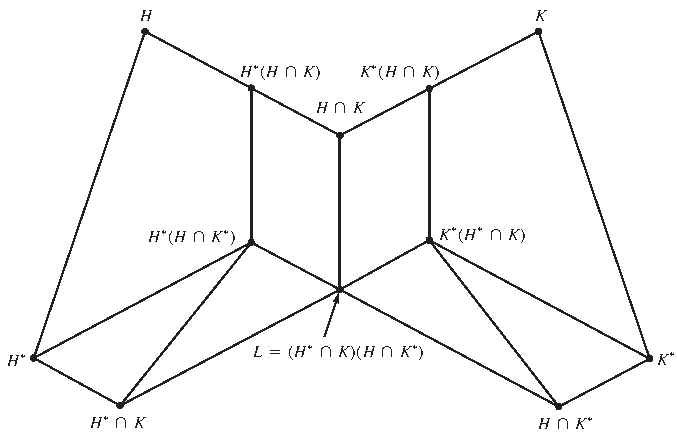
\includegraphics[width=0.929\linewidth,height=.8\textheight,keepaspectratio]{assets/p176_00.pdf}\end{center}
\begin{center}\small\textbf{18.9 Figure}\end{center}
\end{BookFloat}

We now show that \BookInline{H^{\ast }(H\cap K^{\ast })} is a normal subgroup of \BookInline{H^{\ast }(H\cap K).} We let \BookInline{w\in H^{\ast }(H\cap K^{\ast })} and \BookInline{y\in H^{\ast }(H\cap K).} We need to verify that \BookInline{ywy^{- 1}\in H^{\ast }(H\cap K^{\ast }).} By definition\BookInline{,\allowbreak w= h_{1}x} and \BookInline{y\in h_{2}g} for some \BookInline{h_{1},\allowbreak h_{2}\in H^{\ast },\allowbreak x\in H\cap K^{\ast },\allowbreak } and \BookInline{g\in H\cap K.} We write

\begin{center}\begin{adjustbox}{max width=\linewidth}\BookInline{\displaystyle \begin{aligned}ywy^{- 1}&= h_{2}gh_{1}xg^{- 1}h_{2}^{- 1} \\ &= h_{2}(gh_{1}g^{- 1})gxg^{- 1}h_{2}^{- 1} \\ &= h_{2}h_{3}gxg^{- 1}h_{2}^{- 1}\end{aligned}}\end{adjustbox}\end{center}

\noindent for some \BookInline{h_{3}\in H^{\ast }} since \BookInline{H^{\ast }} is a normal subgroup of \BookInline{H.} We note that \BookInline{h_{2}^{- 1}} and \BookInline{h_{2}h_{3}} are both elements of \BookInline{H^{\ast }\leq H^{\ast }(H\cap K^{\ast }).} Furthermore \BookInline{gxg} \BookInline{^ { - 1 } \in K ^ { * }} since \BookInline{g\in K} and \BookInline{K^{\ast }} is a normal subgroup of \BookInline{K.} Also \BookInline{gxg^{- 1}\in H} since both \BookInline{g} and \BookInline{x} are elements of \BookInline{H.} Thus\BookInline{,\allowbreak gxg^{- 1}\in H\cap K^{\ast }\leq K^{\ast }(H\cap K^{\ast }).} So\BookInline{,\allowbreak ywy^{- 1}} is the product of elements in the group \BookInline{H^{\ast }(H\cap K^{\ast }),\allowbreak } which implies that \BookInline{ywy^{- 1}\in H^{\ast }(H\cap K^{\ast }).} Thus we have shown Part 1 of the Theorem.

We use the Second Isomorphism Theorem (16.5) to prove the third part of the Lemma. Let \BookInline{N^{\prime }= H^{\ast }(H\cap K^{\ast })} and \BookInline{H^{\prime }= H\cap K.} So \BookInline{N^{\prime }} is a normal subgroup of \BookInline{H^{\ast }(H\cap K)} and \BookInline{H^{\prime }} is a subgroup of \BookInline{H^{\ast }(H\cup K).} By Lemma \BookInline{16.4N^{\prime }H^{\prime }} is a group and

\begin{center}\begin{adjustbox}{max width=\linewidth}\BookInline{\displaystyle \begin{aligned}N^{\prime }H^{\prime }&= H^{\ast }(H\cap K^{\ast })(H\cap K) \\ &= H^{\ast }(H\cap K).\end{aligned}}\end{adjustbox}\end{center}

\noindent The Second Isomorphism Theorem says that \BookInline{N^{\prime }H^{\prime }/N^{\prime }\simeq H^{\prime }/(H^{\prime }\cap N^{\prime }).} We have

\begin{center}\begin{adjustbox}{max width=\linewidth}\BookInline{\displaystyle N^{\prime }H^{\prime }/N^{\prime }= H^{\ast }(H\cap K)/H^{\ast }(H\cap K^{\ast })}\end{adjustbox}\end{center}

\noindent and

\begin{center}\begin{adjustbox}{max width=\linewidth}\BookInline{\displaystyle H^{\prime }/(H^{\prime }\cap N^{\prime })= (H\cap K)/(H^{\ast }(H\cap K^{\ast })\cap (H\cap K)).}\end{adjustbox}\end{center}

\noindent Exercise 11 in Section 16 shows that

\begin{center}\begin{adjustbox}{max width=\linewidth}\BookInline{\displaystyle H^{\ast }(H\cap K^{\ast })\cap (H\cap K)= (H^{\ast }\cap K)(H\cap K^{\ast }).}\end{adjustbox}\end{center}

\noindent Thus

\begin{center}\begin{adjustbox}{max width=\linewidth}\BookInline{\displaystyle H^{\ast }(H\cap K)/(H^{\ast }(H\cap K^{\ast }))\simeq (H\cap K)/((H^{\ast }\cap K)(H\cap K^{\ast })).}\end{adjustbox}\end{center}

\end{BookBody}

% Source PDF page 177; original printed page 160
\BookSource{177}{160}
\BookNarrativetrue

\begin{BookBody}

By reversing the roles of \BookInline{H} and \BookInline{K(}as well as \BookInline{H^{\ast }} and \BookInline{K^{\ast }),\allowbreak } the proof given above proves Part 2 as well as the other half of Part 3 of the Zassenhaus Lemma\BookInline{.}\BookEnd{\blacklozenge}

\BookLabel{18.11 Theorem} \textbf{(Schreier Theorem)} Two subnormal (normal) series of a group \BookInline{G} have isomorphic refinements.

\BookLabel{\textit{Proof}} Let \BookInline{G} be a group and let

\begin{center}\begin{adjustbox}{max width=\linewidth}\BookInline{\displaystyle \{e\}= H_{0}<H_{1}<H_{2}<\cdots <H_{n}= G(1)}\end{adjustbox}\end{center}

\noindent and

\begin{center}\begin{adjustbox}{max width=\linewidth}\BookInline{\displaystyle \{e\}= K_{0}<K_{1}<K_{2}<\cdots <K_{m}= G(2)}\end{adjustbox}\end{center}

\noindent be two subnormal series for \BookInline{G.} For \BookInline{i} where \BookInline{0\leq i\leq n- 1,\allowbreak } form the chain of groups

\begin{center}\begin{adjustbox}{max width=\linewidth}\BookInline{\displaystyle H_{i}= H_{i}(H_{i+ 1}\cap K_{0})\leq H_{i}(H_{i+ 1}\cap K_{1})\leq \cdots \leq H_{i}(H_{i+ 1}\cap K_{m})= H_{i+ 1}.}\end{adjustbox}\end{center}

\noindent This inserts \BookInline{m- 1} not necessarily distinct groups between \BookInline{H_{i}} and \BookInline{H_{i+ 1}.} If we do this for each \BookInline{i} where \BookInline{0\leq i\leq n- 1} and let \BookInline{H_{i,\allowbreak j}= H_{i}(H_{i+ 1}\cap K_{j}),\allowbreak } then we obtain the chain of groups

\begin{center}\begin{adjustbox}{max width=\linewidth}\BookInline{\displaystyle \begin{aligned}\{e\}&= H_{0,\allowbreak 0}\leq H_{0,\allowbreak 1}\leq H_{0,\allowbreak 2}\leq \cdots \leq H_{0,\allowbreak m- 1}\leq H_{1,\allowbreak 0} \\ &\leq H_{1,\allowbreak 1}\leq H_{1,\allowbreak 2}\leq \cdots \leq H_{1,\allowbreak m- 1}\leq H_{2,\allowbreak 0} \\ &\leq H_{2,\allowbreak 1}\leq H_{2,\allowbreak 2}\leq \cdots \leq H_{2,\allowbreak m- 1}\leq H_{3,\allowbreak 0} \\ &\leq \cdots  \\ &\leq H_{n- 1,\allowbreak 1}\leq H_{n- 1,\allowbreak 2}\leq \cdots \leq H_{n- 1,\allowbreak m- 1}\leq H_{n- 1,\allowbreak m} \\ &= G.(3)\end{aligned}}\end{adjustbox}\end{center}

\noindent This chain (3) contains \BookInline{nm+ 1} not necessarily distinct groups, and \BookInline{H_{i,\allowbreak 0}= H_{i}} for each \BookInline{i.} By the Zassenhaus Lemma, chain (3) is a subnormal chain, that is, each group is normal in the following group. This chain refines the series (1).

In a symmetric fashion, we set \BookInline{K_{j,\allowbreak i}= K_{j}(K_{j+ 1}\cap H_{i})} for \BookInline{0\leq j\leq m- 1} and \BookInline{0\leq i\leq n.} This gives a subnormal chain

\begin{center}\begin{adjustbox}{max width=\linewidth}\BookInline{\displaystyle \begin{aligned}\{e\}&= K_{0,\allowbreak 0}\leq K_{0,\allowbreak 1}\leq K_{0,\allowbreak 2}\leq \cdots \leq K_{0,\allowbreak n- 1}\leq K_{1,\allowbreak 0} \\ &\leq K_{1,\allowbreak 1}\leq K_{1,\allowbreak 2}\leq \cdots \leq K_{1,\allowbreak n- 1}\leq K_{2,\allowbreak 0} \\ &\leq K_{2,\allowbreak 1}\leq K_{2,\allowbreak 2}\leq \cdots \leq K_{2,\allowbreak n- 1}\leq K_{3,\allowbreak 0} \\ &\leq \cdots  \\ &\leq K_{m- 1,\allowbreak 1}\leq K_{m- 1,\allowbreak 2}\leq \cdots \leq K_{m- 1,\allowbreak n- 1}\leq K_{m- 1,\allowbreak n} \\ &= G.(4)\end{aligned}}\end{adjustbox}\end{center}

\noindent This chain (4) contains \BookInline{mn+ 1} not necessarily distinct groups, and \BookInline{K_{j,\allowbreak 0}= K_{j}} for each \BookInline{j.} This chain refines the series (2).

By the Zassenhaus Lemma 18.10, we have

\begin{center}\begin{adjustbox}{max width=\linewidth}\BookInline{\displaystyle H_{i}(H_{i+ 1}\cap K_{j+ 1})/H_{i}(H_{i+ 1}\cap K_{j})\simeq K_{j}(K_{j+ 1}\cap H_{i+ 1})/K_{j}(K_{j+ 1}\cap H_{i}),\allowbreak }\end{adjustbox}\end{center}

\noindent or

\begin{center}\begin{adjustbox}{max width=\linewidth}\BookInline{\displaystyle H_{i,\allowbreak j+ 1}/H_{i,\allowbreak j}\simeq K_{j,\allowbreak i+ 1}/K_{j,\allowbreak i}(5)}\end{adjustbox}\end{center}

\noindent for \BookInline{0\leq i\leq n- 1} and \BookInline{0\leq j\leq m- 1.} The isomorphisms of relation (5) give a one-toone correspondence of isomorphic factor groups between the subnormal chains (3) and (4). To verify this correspondence, note that \BookInline{H_{i,\allowbreak 0}= H_{i}} and \BookInline{H_{i,\allowbreak m}= H_{i+ 1},\allowbreak } while \BookInline{K_{j,\allowbreak 0}= K_{j}} and \BookInline{K_{j,\allowbreak n}= K_{j+ 1}.} Each chain in (3) and (4) contains a rectangular array of \BookInline{mn} symbols \BookInline{\leq.} Each \BookInline{\leq } gives rise to a factor group. The factor groups arising from the \BookInline{r}th\textit{ row} of \BookInline{\leq }’s 
% Source PDF page 178; original printed page 161
\BookSource{178}{161}
in chain (3) correspond to the factor groups arising from the \BookInline{r}th\textit{ column} of \BookInline{\leq }’s in chain (4). Deleting repeated groups from the chains in (3) and (4), we obtain subnormal series of distinct groups that are isomorphic refinements of chains (1) and (2). This establishes the theorem for subnormal series.

\end{BookBody}

\BookNarrativetrue

\begin{BookBody}

For normal series, where all \BookInline{H_{i}} and \BookInline{K_{j}} are normal in \BookInline{G,\allowbreak } we merely observe that all the groups \BookInline{H_{i,\allowbreak j}} and \BookInline{K_{j,\allowbreak i}} formed above are also normal in \BookInline{G,\allowbreak } so the same proof applies. This normality of \BookInline{H_{i,\allowbreak j}} and \BookInline{K_{j,\allowbreak i}} follows at once from the second assertion in Lemma 16.4 and from the fact that intersections of normal subgroups of a group yield normal subgroups\BookInline{.}\BookEnd{\blacklozenge}

\BookTextHeading{\textbf{The Jordan–Ho¨ lder Theorem}  }

\noindent We now come to the real meat of the theory.

\BookLabel{18.12 Definition} A subnormal series \BookInline{\{H_{i}\}} of a group \BookInline{G} is a\textbf{ composition series} if all the factor groups \BookInline{H_{i+ 1}/H_{i}} are simple. A normal series \BookInline{\{H_{i}\}} of \BookInline{G} is a\textbf{ principal} or\textbf{ chief series} if all the factor groups \BookInline{H_{i+ 1}/H_{i}} are simple\BookInline{.}\BookEnd{\blacksquare}

Note that for abelian groups the concepts of composition and principal series coincide. Also, since every normal series is subnormal, every principal series is a composition series for any group, abelian or not.

\BookLabel{18.13 Example} We claim that \BookInline{\mathbb{Z}} has no composition (and also no principal) series. For if

\begin{center}\begin{adjustbox}{max width=\linewidth}\BookInline{\displaystyle \{0\}= H_{0}<H_{1}<\cdots <H_{n- 1}<H_{n}= \mathbb{Z}}\end{adjustbox}\end{center}

\noindent is a subnormal series\BookInline{,\allowbreak H_{1}} must be of the form \BookInline{r\mathbb{Z}} for some \BookInline{r\in \mathbb{Z}^{+ }.} But then \BookInline{H_{1}/H_{0}} is isomorphic to \BookInline{r\mathbb{Z},\allowbreak } which is infinite cyclic with many nontrivial proper normal subgroups, for example\BookInline{,\allowbreak 2r\mathbb{Z}.} Thus \BookInline{\mathbb{Z}} has no composition (and also no principal) series. \BookEnd{\blacktriangle}

\BookLabel{18.14 Example} The series

\begin{center}\begin{adjustbox}{max width=\linewidth}\BookInline{\displaystyle \{e\}<A_{n}<S_{n}}\end{adjustbox}\end{center}

\noindent for \BookInline{n\geq 5} is a composition series (and also a principal series) of \BookInline{S_{n},\allowbreak } because \BookInline{A_{n}/\{e\}} is isomorphic to \BookInline{A_{n},\allowbreak } which is simple for \BookInline{n\geq 5,\allowbreak } and \BookInline{S_{n}/A_{n}} is isomorphic to \BookInline{\mathbb{Z}_{2},\allowbreak } which is simple. Likewise, the two series given in Example 18.7 are composition series (and also principal series) of \BookInline{\mathbb{Z}_{15}.} They are isomorphic, as shown in that example. This illustrates our main theorem, which will be stated shortly\BookInline{.}\BookEnd{\blacktriangle}

Observe that by Theorem \BookInline{13.20,\allowbreak H_{i+ 1}/H_{i}} is simple if and only if \BookInline{H_{i}} is a maximal normal subgroup of \BookInline{H_{i+ 1}.} Thus for a composition series, each \BookInline{H_{i}} must be a maximal normal subgroup of \BookInline{H_{i+ 1}.} \textit{To form} \BookInline{a} \textit{composition series of} \BookInline{a} \textit{group} \BookInline{G,\allowbreak } \textit{we just} \BookInline{hunt} \textit{for} \BookInline{a} \textit{maximal normal subgroup} \BookInline{H_{n- 1}} \textit{of} \BookInline{G,\allowbreak } \textit{then for} \BookInline{a} \textit{maximal normal subgroup} \BookInline{H_{n- 2}} \textit{of} \BookInline{H_{n- 1},\allowbreak } \textit{and so on}.\textit{ If this process terminates in} \BookInline{a} \textit{finite number of steps, we have} \BookInline{a} \textit{composition series}. Note that by Theorem 13.20, a composition series cannot have any further refinement.\textit{ To form} \BookInline{a} \textit{principal series, we have to} \BookInline{hunt} \textit{for} \BookInline{a} \textit{maximal normal} \textit{subgroup} \BookInline{H_{n- 1}} \textit{of} \BookInline{G,\allowbreak } \textit{then for} \BookInline{a} \textit{maximal normal subgroup} \BookInline{H_{n- 2}} \textit{of} \BookInline{H_{n- 1}} \textit{that is also} \textit{normal in} \BookInline{G,\allowbreak } \textit{and so on}. The main theorem is as follows.

\BookLabel{18.15 Theorem} \textbf{(Jordan–Ho¨lder Theorem)} Any two composition (principal) series of a group \BookInline{G} are isomorphic.

\BookLabel{\textit{Proof}} Let \BookInline{\{H_{i}\}} and \BookInline{\{K_{i}\}} be two composition (principal) series of \BookInline{G.} By Theorem 18.11, they have isomorphic refinements. But since all factor groups are already simple,

\end{BookBody}

% Source PDF page 179; original printed page 162
\BookSource{179}{162}
\BookNarrativetrue

\begin{BookBody}

\noindent Theorem 13.20 shows that neither series has any further refinement. Thus \BookInline{\{H_{i}\}} and \BookInline{\{K_{i}\}} must already be isomorphic\BookInline{.}\BookEnd{\blacklozenge}

For a finite group, we should regard a composition series as a type of factorization of the group into simple factor groups, analogous to the factorization of a positive integer into primes. In both cases, the factorization is unique, up to the order of the factors.

\BookLabel{18.16 Example} We illustrate the analogy between factoring integers and composition series with an example. Let \BookInline{n\in \mathbb{Z}^{+ }.} We factor \BookInline{n} into its prime factors \BookInline{n= p_{1}p_{2}p_{3}...p_{k},\allowbreak } where the prime factors may be repeated and they are in any order. The series

\begin{center}\begin{adjustbox}{max width=\linewidth}\BookInline{\displaystyle \{0\}<\langle p_{1}p_{2}p_{3}\cdots p_{k- 1}\rangle <\langle p_{1}p_{2}p_{3}\cdots p_{k- 2}\rangle <\langle p_{1}p_{2}p_{3}\cdots p_{k- 3}\rangle <\cdots <\langle p_{1}\rangle <\mathbb{Z}_{n}}\end{adjustbox}\end{center}

\noindent is a composition series since the factor groups are isomorphic with \BookInline{\mathbb{Z}_{p_{k}},\allowbreak \mathbb{Z}_{p_{k- 1}},\allowbreak \mathbb{Z}_{p_{k- 2}},\allowbreak...}, \BookInline{\mathbb{Z}_{p_{1}}}, which are all simple. For each choice of ordering the prime numbers \BookInline{p_{1},\allowbreak p_{2},\allowbreak...,\allowbreak p_{k}} we get a different composition series, but they are all isomorphic since the factor groups are \BookInline{\mathbb{Z}_{p_{1}},\allowbreak \mathbb{Z}_{p_{2}},\allowbreak...,\allowbreak \mathbb{Z}_{p_{k}}} in some order\BookInline{.}\BookEnd{\blacktriangle}

\BookTextHeading{\ensuremath{\blacksquare} \textbf{HISTORICAL NOTE}  }

\noindent This first appearance of what became the Jordan–Ho¨lder theorem occurred in 1869 in a commentary on the work of Galois by the brilliant French algebraist Camille Jordan (1838– 1922). The context of its appearance is the study of permutation groups associated with the roots of polynomial equations. Jordan asserted that even though the sequence of normal subgroups \BookInline{G,\allowbreak I,\allowbreak J,\allowbreak \cdots } of the group of the equation is not necessarily unique, nevertheless the sequence of indices of this composition series is unique. Jordan gave a proof in his monumental 1870\textit{ Treatise on Substitutions and Algebraic} \textit{Equations}. This latter work, though restricted to what we now call permutation groups, remained the standard treatise on group theory for many years.

The Ho¨lder part of the theorem, that the sequence of factor groups in a composition series is unique up to order, was due to Otto Ho¨lder (1859– 1937), who played a very important role in the development of group theory once the completely abstract definition of a group had been given. Among his other contributions, he gave the first abstract definition of a “factor group” and determined the structure of all finite groups of square-free order.

\BookLabel{18.17 Theorem} If \BookInline{G} has a composition (principal) series, and if \BookInline{N} is a proper normal subgroup of \BookInline{G,\allowbreak } then there exists a composition (principal) series containing \BookInline{N.}

\BookLabel{\textit{Proof}} The series

\begin{center}\begin{adjustbox}{max width=\linewidth}\BookInline{\displaystyle \{e\}<N<G}\end{adjustbox}\end{center}

\noindent is both a subnormal and a normal series. Since \BookInline{G} has a composition series \BookInline{\{H_{i}\},\allowbreak } then by Theorem 18.11 there is a refinement of \BookInline{\{e\}<N<G} to a subnormal series isomorphic to a refinement of \BookInline{\{H_{i}\}.} But as a composition series\BookInline{,\allowbreak \{H_{i}\}} can have no further refinement. Thus \BookInline{\{e\}<N<G} can be refined to a subnormal series all of whose factor groups are simple, that is, to a composition series. A similar argument holds if we start with a principal series \BookInline{\{K_{j}\}} of \BookInline{G.}\BookEnd{\blacklozenge}

\BookLabel{18.18 Example} A composition (and also a principal) series of \BookInline{\mathbb{Z}_{4}\times \mathbb{Z}_{9}} containing \BookInline{\langle (0,\allowbreak 1)\rangle } is

\begin{center}\begin{adjustbox}{max width=\linewidth}\BookInline{\displaystyle \{(0,\allowbreak 0)\}<\langle (0,\allowbreak 3)\rangle <\langle (0,\allowbreak 1)\rangle <\langle 2\rangle \times \langle 1\rangle <\langle 1\rangle \times \langle 1\rangle = \mathbb{Z}_{4}\times \mathbb{Z}_{9}.}\end{adjustbox}\end{center} \BookEnd{\blacktriangle}

\end{BookBody}

% Source PDF page 180; original printed page 163
\BookSource{180}{163}
\BookNarrativetrue

\begin{BookBody}

The next definition is basic to the characterization of those polynomial equations whose solutions can be expressed in terms of radicals.

\BookLabel{18.19 Definition} A group \BookInline{G} is\textbf{ solvable} if it has a composition series \BookInline{\{H_{i}\}} such that all factor groups \BookInline{H_{i+ 1}/H_{i}} are abelian\BookInline{.}\BookEnd{\blacksquare}

By the Jordan–Ho¨lder theorem, we see that for a solvable group,\textit{ every} composition series \BookInline{\{H_{i}\}} must have abelian factor groups \BookInline{H_{i+ 1}/H_{i}.}

\BookLabel{18.20 Example} The group \BookInline{S_{3}} is solvable, because the composition series

\begin{center}\begin{adjustbox}{max width=\linewidth}\BookInline{\displaystyle \{e\}<A_{3}<S_{3}}\end{adjustbox}\end{center}

\noindent has factor groups isomorphic to \BookInline{\mathbb{Z}_{3}} and \BookInline{\mathbb{Z}_{2},\allowbreak } which are abelian. The group \BookInline{S_{5}} is not solvable, for since \BookInline{A_{5}} is simple, the series

\begin{center}\begin{adjustbox}{max width=\linewidth}\BookInline{\displaystyle \{e\}<A_{5}<S_{5}}\end{adjustbox}\end{center}

\noindent is a composition series, and \BookInline{A_{5}/\{e\},\allowbreak } which is isomorphic to \BookInline{A_{5},\allowbreak } is not abelian.\textit{ This group} \BookInline{A_{5}} \textit{of order} 60\textit{ can be shown to be the smallest group that is not solvable}. This fact is closely connected with the fact that a polynomial equation of degree 5 is not in general solvable by radicals, but a polynomial equation of degree \BookInline{\leq 4} is\BookInline{.}\BookEnd{\blacktriangle}

\BookTextHeading{\textbf{The Ascending Central Series}  }

\noindent We mention one subnormal series for a group \BookInline{G} that can be formed using centers of groups. Recall from Section 13 that the center \BookInline{Z(G)} of a group \BookInline{G} is defined by

\begin{center}\begin{adjustbox}{max width=\linewidth}\BookInline{\displaystyle Z(G)= \{z\in G\mid zg= gz\;\text{for all}\;g\in G\},\allowbreak }\end{adjustbox}\end{center}

\noindent and that \BookInline{Z(G)} is a normal subgroup of \BookInline{G.} If we have the table for a finite group \BookInline{G,\allowbreak } it is easy to find the center. An element \BookInline{a} is in the center of \BookInline{G} if and only if the row with header \BookInline{a} and the column with header \BookInline{a} list the elements of \BookInline{G} in the same order.

Now let \BookInline{G} be a group, and let \BookInline{Z(G)} be the center of \BookInline{G.} Since \BookInline{Z(G)} is normal in \BookInline{G,\allowbreak } we can form the factor group \BookInline{G/Z(G)} and find the center \BookInline{Z(G/Z(G))} of this factor group. Since \BookInline{Z(G/Z(G))} is normal in \BookInline{G/Z(G),\allowbreak } if \BookInline{\gamma:G\to G/Z(G)} is the canonical map, then by Theorem \BookInline{13.18,\allowbreak \gamma ^{- 1}[Z(G/Z(G))]} is a normal subgroup \BookInline{Z_{1}(G)} of \BookInline{G.} We can then form the factor group \BookInline{G/Z_{1}(G)} and find its center, take \BookInline{(\gamma _{1})^{- 1}} of it to get \BookInline{Z_{2}(G),\allowbreak } and so on.

\BookLabel{18.21 Definition} The series

\begin{center}\begin{adjustbox}{max width=\linewidth}\BookInline{\displaystyle \{e\}\leq Z(G)\leq Z_{1}(G)\leq Z_{2}(G)\leq \cdots}\end{adjustbox}\end{center}

\noindent described in the preceding discussion is the\textbf{ ascending central series of the group} \BookInline{G.} \BookEnd{\blacksquare}

\BookLabel{18.22 Example} For \BookInline{n\geq 3,\allowbreak } the center of \BookInline{S_{n}} is just the identity \BookInline{\iota.} Thus the ascending central series of \BookInline{S_{n}} is

\begin{center}\begin{adjustbox}{max width=\linewidth}\BookInline{\displaystyle \{\iota \}\leq \{\iota \}\leq \{\iota \}\leq ....}\end{adjustbox}\end{center}

\noindent The center of the dihedral group \BookInline{D_{4}} is \BookInline{\{\iota,\allowbreak \rho ^{2}\}.} The factor group \BookInline{D_{4}/\{\iota,\allowbreak \rho ^{2}\}} has order 4, and each element has order 1 or 2, so \BookInline{D_{4}/\{\iota,\allowbreak \rho ^{2}\}} is isomorphic with the Klein 4-group, which is abelian. Therefore the center of \BookInline{D_{4}/\{\iota,\allowbreak \rho ^{2}\}} is the whole group, and the central series for \BookInline{D_{4}} is

\begin{center}\begin{adjustbox}{max width=\linewidth}\BookInline{\displaystyle \{\iota \}\leq \{\iota ,\allowbreak \rho ^{2}\}\leq D_{4}\leq D_{4}\leq D_{4}\leq ....}\end{adjustbox}\end{center} \BookEnd{\blacktriangle}

\end{BookBody}

% Source PDF page 181; original printed page 164
\BookSource{181}{164}
\BookNarrativefalse

\begin{BookBody}

\BookExerciseTitle{18}

\BookTextHeading{\textbf{Computations}}

\noindent In Exercises 1 through 5, give isomorphic refinements of the two series.

\BookExercise{1.}{\BookInline{\{0\}<10\mathbb{Z}<\mathbb{Z}} and \BookInline{\{0\}<25\mathbb{Z}<\mathbb{Z}}}

\BookExercise{2.}{\BookInline{\{0\}<60\mathbb{Z}<20\mathbb{Z}<\mathbb{Z}} and \BookInline{\{0\}<245\mathbb{Z}<49\mathbb{Z}<\mathbb{Z}}}

\BookExercise{3.}{\BookInline{\{0\}<\langle 9\rangle <\mathbb{Z}_{54}} and \BookInline{\{0\}<\langle 2\rangle <\mathbb{Z}_{54}}}

\BookExercise{4.}{\BookInline{\{0\}<\langle 9\rangle <\langle 3\rangle <\mathbb{Z}_{72}} and \BookInline{\{0\}<\langle 36\rangle <\langle 12\rangle <\mathbb{Z}_{72}}}

\BookExercise{5.}{\BookInline{\{(0,\allowbreak 0)\}<(60\mathbb{Z})\times \mathbb{Z}<(10\mathbb{Z})\times \mathbb{Z}<\mathbb{Z}\times \mathbb{Z}} and \BookInline{\{(0,\allowbreak 0)\}<\mathbb{Z}\times (80\mathbb{Z})<\mathbb{Z}\times (20\mathbb{Z})<\mathbb{Z}\times \mathbb{Z}}}

\BookExercise{6.}{Find all composition series of \BookInline{\mathbb{Z}_{90}} and show that they are isomorphic.}

\BookExercise{7.}{Find all composition series of \BookInline{\mathbb{Z}_{48}} and show that they are isomorphic.}

\BookExercise{8.}{Find all composition series of \BookInline{\mathbb{Z}_{5}\times \mathbb{Z}_{5}.}}

\BookExercise{9.}{Find all composition series of \BookInline{S_{3}\times \mathbb{Z}_{2}.}}

\BookExercise{10.}{Find all composition series of \BookInline{\mathbb{Z}_{2}\times \mathbb{Z}_{5}\times \mathbb{Z}_{7}.}}

\BookExercise{11.}{Find the center of \BookInline{S_{3}\times \mathbb{Z}_{4}.}}

\BookExercise{12.}{Find the center of \BookInline{S_{3}\times D_{4}.}}

\BookExercise{13.}{Find the ascending central series of \BookInline{S_{3}\times \mathbb{Z}_{4}.}}

\BookExercise{14.}{Find the ascending central series of \BookInline{S_{3}\times D_{4}.}}

\BookTextHeading{\textbf{Concepts}}

\noindent In Exercises 15 and 16, correct the definition of the italicized term without reference to the text, if correction is needed, so that it is in a form acceptable for publication.

\BookExercise{15.}{A\textit{ composition series} of a group \BookInline{G} is a finite sequence}

\begin{center}\begin{adjustbox}{max width=\linewidth}\BookInline{\displaystyle \{e\}= H_{0}<H_{1}<H_{2}<\cdots <H_{n- 1}<H_{n}= G}\end{adjustbox}\end{center}

of subgroups of \BookInline{G} such that \BookInline{H_{i}} is a maximal normal subgroup of \BookInline{H_{i+ 1}} for \BookInline{i= 0,\allowbreak 1,\allowbreak 2,\allowbreak \cdots,\allowbreak n- 1.}

\BookExercise{16.}{A\textit{ solvable group} is one that has a composition series of abelian groups.}

\BookExercise{17.}{Determine whether each of the following is true or false.}

\BookExercise{a.}{Every normal series is also subnormal.}

\BookExercise{b.}{Every subnormal series is also normal.}

\BookExercise{c.}{Every principal series is a composition series.}

\BookExercise{d.}{Every composition series is a principal series.}

\BookExercise{e.}{Every abelian group has exactly one composition series.}

\BookExercise{f.}{Every finite group has a composition series.}

\BookExercise{g.}{A group is solvable if and only if it has a composition series with simple factor groups.}

\BookExercise{h.}{\textbf{h}\BookInline{.S_{7}} is a solvable group.}

\BookExercise{i.}{The Jordan–Ho¨lder theorem has some similarity with the Fundamental Theorem of Arithmetic, which states that every positive integer greater than 1 can be factored into a product of primes uniquely up to order.}

\BookExercise{j.}{Every finite group of prime order is solvable.}

\BookExercise{18.}{Find a composition series of \BookInline{S_{3}\times S_{3}.} Is \BookInline{S_{3}\times S_{3}} solvable?}

\BookExercise{19.}{Is the dihedral group \BookInline{D_{4}} solvable?}

\BookExercise{20.}{Let \BookInline{G} be \BookInline{\mathbb{Z}_{36}.} Refer to the proof of Theorem 18.11. Let the subnormal series (1) be}

\begin{center}\begin{adjustbox}{max width=\linewidth}\BookInline{\displaystyle \{0\}<\langle 12\rangle <\langle 3\rangle <\mathbb{Z}_{36}}\end{adjustbox}\end{center}

and let the subnormal series (2) be

\begin{center}\begin{adjustbox}{max width=\linewidth}\BookInline{\displaystyle \{0\}<\langle 18\rangle <\mathbb{Z}_{36}.}\end{adjustbox}\end{center}

\end{BookBody}

% Source PDF page 182; original printed page 165
\BookSource{182}{165}
\BookNarrativefalse

\begin{BookBody}

Find chains (3) and (4) and exhibit the isomorphic factor groups as described in the proof. Write chains (3) and (4) in the rectangular array shown in the text.

\BookExercise{21.}{Repeat Exercise 20 for the group \BookInline{\mathbb{Z}_{24}} with the subnormal series (1)}

\begin{center}\begin{adjustbox}{max width=\linewidth}\BookInline{\displaystyle \{0\}<\langle 12\rangle <\langle 4\rangle <\mathbb{Z}_{24}}\end{adjustbox}\end{center}

and (2)

\begin{center}\begin{adjustbox}{max width=\linewidth}\BookInline{\displaystyle \{0\}<\langle 6\rangle <\langle 3\rangle <\mathbb{Z}_{24}.}\end{adjustbox}\end{center}

\BookTextHeading{\textbf{Theory}}

\BookExercise{22.}{Let \BookInline{H^{\ast },\allowbreak H,\allowbreak } and \BookInline{K} be subgroups of \BookInline{G} with \BookInline{H^{\ast }} normal in \BookInline{H.} Show that \BookInline{H^{\ast }\cap K} is normal in \BookInline{H\cap K.}}

\BookExercise{23.}{Show that if}

\begin{center}\begin{adjustbox}{max width=\linewidth}\BookInline{\displaystyle H_{0}= \{e\}<H_{1}<H_{2}<\cdots <H_{n}= G}\end{adjustbox}\end{center}

is a subnormal (normal) series for a group \BookInline{G,\allowbreak } and if \BookInline{H_{i+ 1}/H_{i}} is of finite order \BookInline{s_{i+ 1},\allowbreak } then \BookInline{G} is of finite order \BookInline{s_{1}s_{2}\cdots s_{n}.}

\BookExercise{24.}{Show that an infinite abelian group can have no composition series. [\textit{Hint:} Use Exercise 23, together with the fact that an infinite abelian group always has a proper nontrivial subgroup.]}

\BookExercise{25.}{Show that a finite direct product of solvable groups is solvable.}

\BookExercise{26.}{Show that if \BookInline{H\unlhd G} is a normal subgroup\BookInline{,\allowbreak H} is solvable, and \BookInline{G/H} is solvable, then \BookInline{G} is solvable.}

\BookExercise{27.}{Show that for \BookInline{n\geq 3,\allowbreak D_{n}} is solvable.}

\BookExercise{28.}{Show that a subgroup \BookInline{K} of a solvable group \BookInline{G} is solvable. [\textit{Hint:} Let \BookInline{H_{0}= \{e\}<H_{1}<\cdots <H_{n}= G} be a composition series for \BookInline{G.} Show that the distinct groups among \BookInline{K\cap H_{i}} for \BookInline{i= 0,\allowbreak \cdots,\allowbreak n} form a composition series for \BookInline{K.} Observe that}

\begin{center}\begin{adjustbox}{max width=\linewidth}\BookInline{\displaystyle (K\cap H_{i})/(K\cap H_{i- 1})\simeq [H_{i- 1}(K\cap H_{i})]/[H_{i- 1}],\allowbreak }\end{adjustbox}\end{center}

by Theorem 16.5, with \BookInline{H= K\cap H_{i}} and \BookInline{N= H_{i- 1},\allowbreak } and that \BookInline{H_{i- 1}(K\cap H_{i})\leq H_{i}.]}

\BookExercise{29.}{Let \BookInline{H_{0}= \{e\}<H_{1}<\cdots <H_{n}= G} be a composition series for a group \BookInline{G.} Let \BookInline{N} be a normal subgroup of \BookInline{G,\allowbreak } and suppose that \BookInline{N} is a simple group. Show that the distinct groups among \BookInline{H_{0},\allowbreak H_{i}N} for \BookInline{i= 0,\allowbreak \cdots,\allowbreak n} also form a composition series for \BookInline{G.[}\textit{Hint}\BookInline{:H_{i}N} is a group by Lemma 16.4. Show that \BookInline{H_{i- 1}N} is normal in \BookInline{H_{i}N.} By Theorem 16.5}

\begin{center}\begin{adjustbox}{max width=\linewidth}\BookInline{\displaystyle (H_{i}N)/(H_{i- 1}N)\simeq H_{i}/[H_{i}\cap (H_{i- 1}N)],\allowbreak }\end{adjustbox}\end{center}

and the latter group is isomorphic to

\begin{center}\begin{adjustbox}{max width=\linewidth}\BookInline{\displaystyle [H_{i}/H_{i- 1}]/[(H_{i}\cap (H_{i- 1}N))/H_{i- 1}],\allowbreak }\end{adjustbox}\end{center}

by Theorem 16.8. But \BookInline{H_{i}/H_{i- 1}} is simple.]

\BookExercise{30.}{Let \BookInline{G} be a group, and let \BookInline{H_{0}= \{e\}<H_{1}<\cdots <H_{n}= G} be a composition series for \BookInline{G.} Let \BookInline{N} be a normal subgroup of \BookInline{G,\allowbreak } and let \BookInline{\gamma:G\to G/N} be the canonical map. Show that the distinct groups among \BookInline{\gamma [H_{i}]} for \BookInline{i= 0,\allowbreak \cdots,\allowbreak n,\allowbreak } form a composition series for \BookInline{G/N.[}\textit{Hint:} Observe that the map}

\begin{center}\begin{adjustbox}{max width=\linewidth}\BookInline{\displaystyle \psi :H_{i}N\to \gamma [H_{i}]/\gamma [H_{i- 1}]}\end{adjustbox}\end{center}

defined by

\begin{center}\begin{adjustbox}{max width=\linewidth}\BookInline{\displaystyle \psi (h_{i}n)= \gamma (h_{i}n)\gamma [H_{i- 1}]}\end{adjustbox}\end{center}

is a homomorphism with kernel \BookInline{H_{i- 1}N.} By Theorem 16.2.

\begin{center}\begin{adjustbox}{max width=\linewidth}\BookInline{\displaystyle \gamma [H_{i}]/\gamma [H_{i- 1}]\simeq (H_{i}N)/(H_{i- 1}N).}\end{adjustbox}\end{center}

Proceed via Theorem 16.5, as shown in the hint for Exercise 29.]

\BookExercise{31.}{Prove that a homomorphic image of a solvable group is solvable. [\textit{Hint:} Apply Exercise 30 to get a composition series for the homomorphic image. The hints for Exercises 29 and 30 then show how the factor groups of this composition series in the image look.]}

\BookExercise{32.}{Prove that a finite \BookInline{p-}group is solvable.}

\end{BookBody}
\ifdefined\BookMaster\let\BookFinish\relax\else\def\BookFinish{\end{document}}\fi\BookFinish

\clearpage
% !TeX program = xelatex
\ifdefined\BookMaster\else
\documentclass[11pt,oneside]{article}
% !TeX program = xelatex
\usepackage[b5paper,left=22mm,right=22mm,top=20mm,bottom=22mm,footskip=11mm]{geometry}
\usepackage{fontspec}
\setmainfont{TeX Gyre Termes}
\setsansfont{TeX Gyre Heros}
\usepackage{amsmath,amssymb,mathtools,amsthm}
\renewcommand{\cdots}{\mathinner{\cdotp\cdotp\cdotp}}
\usepackage{graphicx,adjustbox,array,booktabs,longtable,multirow,enumitem,changepage,needspace}
\usepackage[table]{xcolor}
\usepackage{fancyhdr}
\raggedbottom
\interfootnotelinepenalty=10000
\newcommand{\BookFootnote}[2]{\begingroup\renewcommand{\thefootnote}{\fnsymbol{footnote}}\footnote[#1]{#2}\endgroup}
\newcommand{\BookFootnoteMark}[1]{\begingroup\renewcommand{\thefootnote}{\fnsymbol{footnote}}\footnotemark[#1]\endgroup}
\newcommand{\BookFootnoteText}[2]{\begingroup\renewcommand{\thefootnote}{\fnsymbol{footnote}}\footnotetext[#1]{#2}\endgroup}
\newenvironment{BookFloat}[1]{\par\addvspace{.6\baselineskip}\noindent\def\BookFloatID{#1}\begin{minipage}{\linewidth}\phantomsection\label{bookfloat:#1:start}}{\phantomsection\label{bookfloat:\BookFloatID:end}\end{minipage}\par\addvspace{.6\baselineskip}}

\usepackage[unicode,hidelinks]{hyperref}
\pagestyle{fancy}
\fancyhf{}
\newcommand{\BookFooter}{}
\fancyfoot[L]{\parbox[b]{\dimexpr\textwidth-15mm}{\footnotesize\BookFooter}}
\fancyfoot[R]{\footnotesize\thepage}
\renewcommand{\headrulewidth}{0pt}
\renewcommand{\footrulewidth}{0pt}
\setlength{\parindent}{0pt}
\setlength{\parskip}{0.2em}
\setlength{\emergencystretch}{3em}
\setlist{nosep,leftmargin=1.7em,labelsep=.65em}
\newif\ifBookNarrative
\BookNarrativetrue
\newenvironment{BookBody}{\setlength{\parindent}{0pt}}{}
\newcommand{\BookStatement}[1]{\par\addvspace{.6\baselineskip}\noindent #1\enspace\ignorespaces}
\newcommand{\BookLabel}[1]{\par\addvspace{.6\baselineskip}\needspace{3\baselineskip}\noindent\textbf{#1}\quad\ignorespaces}
\newcommand{\BookHeading}[1]{\par\addvspace{\baselineskip}\needspace{4\baselineskip}\noindent{\large\bfseries #1}\par\medskip}
\newcommand{\BookSubheading}[1]{\par\addvspace{.7\baselineskip}\needspace{3\baselineskip}\noindent{\bfseries #1}\par\smallskip}
\newcommand{\BookTextHeading}[1]{\par\addvspace{.7\baselineskip}\needspace{3\baselineskip}\noindent #1\par\smallskip}
\newcommand{\BookSectionTitle}[2]{\par\addvspace{1.2\baselineskip}\needspace{5\baselineskip}\noindent\colorbox{gray!25}{\sffamily\bfseries\small SECTION #1}\quad{\large\bfseries #2}\par\medskip}
\newcommand{\BookExerciseTitle}[1]{\par\addvspace{\baselineskip}\needspace{4\baselineskip}\noindent{\color{gray}\rule{1.5mm}{1.5mm}}\enspace{\large\bfseries Exercises #1}\par\medskip}
\newcommand{\BookBullet}[1]{\begin{list}{\textbullet}{\setlength{\leftmargin}{1.7em}\setlength{\labelwidth}{1em}\setlength{\labelsep}{.7em}\setlength{\topsep}{0pt}\setlength{\parsep}{0pt}\setlength{\itemsep}{0pt}}\item #1\end{list}}
\newcommand{\BookExercise}[2]{\begin{list}{\textbf{#1}}{\setlength{\leftmargin}{2.2em}\setlength{\labelwidth}{1.5em}\setlength{\labelsep}{.7em}\setlength{\topsep}{.15em}\setlength{\parsep}{0pt}\setlength{\itemsep}{0pt}}\item #2\end{list}}
\newcommand{\BookEnd}[1]{\unskip\nobreak\hfill\ensuremath{#1}}
\newcommand{\BookSource}[2]{\phantomsection\label{sourcepage:#1}} % Source-page anchors, retained through reflow.
\usepackage{multicol}
\usepackage{tikz}
\newcommand{\BookPartEntry}[2]{\par\noindent\makebox[17mm][l]{\bfseries Section #1}#2\par}
\newcommand{\BookPartTitle}[3]{\par\bigskip\noindent\begin{tikzpicture}\node[anchor=north west,inner sep=0pt,outer sep=0pt] (bookpart) at (0,0) {\begin{minipage}{\dimexpr\linewidth-.5pt}\hspace*{26mm}\begin{minipage}[t]{\dimexpr\linewidth-26mm}\begin{adjustbox}{max width=\linewidth}{\fontsize{20}{24}\selectfont\bfseries #2}\end{adjustbox}\par\vspace{6mm}\hrule\vspace{6mm}{\sffamily\footnotesize\setlength{\parskip}{.3em}#3}\vspace{3mm}\end{minipage}\end{minipage}};\path[shade,top color=gray!60,bottom color=white] (0,0) rectangle ([xshift=24mm]bookpart.south west);\node[anchor=north,font=\sffamily\bfseries\small] at (12mm,-2mm) {PART};\node[anchor=north,font=\sffamily\bfseries\Huge] at (12mm,-7mm) {#1};\end{tikzpicture}\par\bigskip}
\newsavebox{\BookMathBox}
\makeatletter
\newcommand{\BookInline}[1]{\leavevmode\hskip0pt\relax\begingroup\in@{\begin}{#1}\ifin@\sbox{\BookMathBox}{\(#1\)}\ifdim\wd\BookMathBox>\dimexpr\linewidth-1em\relax\resizebox{\dimexpr\linewidth-1em\relax}{!}{\usebox{\BookMathBox}}\else\(#1\)\fi\else\in@{\left}{#1}\ifin@\sbox{\BookMathBox}{\(#1\)}\ifdim\wd\BookMathBox>\dimexpr\linewidth-1em\relax\resizebox{\dimexpr\linewidth-1em\relax}{!}{\usebox{\BookMathBox}}\else\(#1\)\fi\else\(#1\)\fi\fi\endgroup\hskip0pt\relax}
\makeatother
\DeclareMathOperator{\Aut}{Aut}
\DeclareMathOperator{\End}{End}
\DeclareMathOperator{\Hom}{Hom}
\DeclareMathOperator{\GF}{GF}
\DeclareMathOperator{\irr}{irr}
\DeclareMathOperator{\lt}{lt}
\DeclareMathOperator{\lp}{lp}
\providecommand{\textcircled}[1]{\textnormal{(#1)}}

\begin{document}
\fi
\renewcommand{\BookFooter}{Section 19 Free Abelian Groups}
\pdfbookmark[0]{Section 19 Free Abelian Groups}{19_free_abelian_groups}
\ifdefined\BookMaster\else\setcounter{page}{166}\fi
% Source PDF page 183; original printed page 166
\BookSource{183}{166}
\BookNarrativetrue

\begin{BookBody}

\BookSectionTitle{19}{Free Abelian Groups}

\noindent In this section we introduce the concept of free abelian groups and prove some results concerning them. The section concludes with a demonstration of the Fundamental Theorem of Finitely Generated Abelian Groups (Theorem 9.12).

\BookTextHeading{\textbf{Free Abelian Groups}  }

\noindent We should review the notions of a generating set for a group \BookInline{G} and a finitely generated group, as given in Section 7. In this section we shall deal exclusively with abelian groups and use the standard additive notations as follows:

0 for the identity\BookInline{,\allowbreak + } for the operation,

\begin{center}\begin{adjustbox}{max width=\linewidth}\BookInline{\displaystyle \left. { \begin{array} { l } { n a = { \underbrace { a + a + \cdots + a } _ { n { \mathrm { ~ s u m m a n a d s } } } } } \\ { - n a = { \underbrace { ( - a ) + ( - a ) + \cdots + ( - a ) } _ { n { \mathrm { ~ s u m m a n a d s } } } } } \end{array} } \right\} { \mathrm { ~ f o r } } \; n \in \mathbb { Z } ^ { + } \; { \mathrm { a n d } } \; a \in G . }\end{adjustbox}\end{center}

\BookInline{0a= 0} for the first 0 in \BookInline{\mathbb{Z}} and the second in \BookInline{G.}

\noindent We shall continue to use the symbol \BookInline{\times } for direct product of groups rather than change to direct sum notation.

Notice that \BookInline{\{(1,\allowbreak 0),\allowbreak (0,\allowbreak 1)\}} is a generating set for the group \BookInline{\mathbb{Z}\times \mathbb{Z}} since \BookInline{(n,\allowbreak m)= n(1,\allowbreak 0)+ m(0,\allowbreak 1)} for any \BookInline{(n,\allowbreak m)} in \BookInline{\mathbb{Z}\times \mathbb{Z}.} This generating set has the property that each element of \BookInline{\mathbb{Z}\times \mathbb{Z}} can be\textit{ uniquely} expressed in the form \BookInline{n(1,\allowbreak 0)+ m(0,\allowbreak 1).} That is, the coefficients \BookInline{n} and \BookInline{m} in \BookInline{\mathbb{Z}} are unique.

\BookLabel{19.1 Theorem} Let \BookInline{X} be a subset of a nonzero abelian group \BookInline{G.} The following conditions on \BookInline{X} are equivalent.

\BookExercise{1.}{Each nonzero element \BookInline{a} in \BookInline{G} can be expressed\textit{ uniquely} (up to order of summands) in the form \BookInline{a= n_{1}x_{1}+ n_{2}x_{2}+ \cdots + n_{r}x_{r}} for \BookInline{n_{i}\neq 0} in \BookInline{\mathbb{Z}} and distinct \BookInline{x_{i}} in \BookInline{X.}}

\BookExercise{2.}{\BookInline{X} generates \BookInline{G,\allowbreak } and \BookInline{n_{1}x_{1}+ n_{2}x_{2}+ \cdots + n_{r}x_{r}= 0} for \BookInline{n_{i}\in \mathbb{Z}} and distinct \BookInline{x_{i}\in X} if and only if \BookInline{n_{1}= n_{2}= \cdots = n_{r}= 0.}}

\BookLabel{\textit{Proof}} Suppose Condition 1 is true. Since \BookInline{G\neq \{0\},\allowbreak } we have \BookInline{X\neq \{0\}.} It follows from 1 that \BookInline{0\not \in X,\allowbreak } for if \BookInline{x_{i}= 0} and \BookInline{x_{j}\neq 0,\allowbreak } then \BookInline{x_{j}= x_{i}+ x_{j},\allowbreak } which would contradict the uniqueness of the expression for \BookInline{x_{j}.} From Condition \BookInline{1,\allowbreak X} generates \BookInline{G,\allowbreak } and \BookInline{n_{1}x_{1}+ n_{2}x_{2}+ \cdots + } \BookInline{n_{r}x_{r}= 0} if \BookInline{n_{1}= n_{2}= \cdots = n_{r}= 0.} Suppose that \BookInline{n_{1}x_{1}+ n_{2}x_{2}+ \cdots + n_{r}x_{r}= 0} with some \BookInline{n_{i}\neq 0;} by dropping terms with zero coefficients and renumbering, we can assume all \BookInline{n_{i}\neq 0.} Then

\begin{center}\begin{adjustbox}{max width=\linewidth}\BookInline{\displaystyle \begin{aligned}x_{1}&= x_{1}+ (n_{1}x_{1}+ n_{2}x_{2}+ \cdots + n_{r}x_{r}) \\ &= (n_{1}+ 1)x_{1}+ n_{2}x_{2}+ \cdots + n_{r}x_{r},\allowbreak \end{aligned}}\end{adjustbox}\end{center}

\noindent which gives two ways of writing \BookInline{x_{1}\neq 0,\allowbreak } contradicting the uniqueness assumption in Condition 1. Thus Condition 1 implies Condition 2.

We now show that Condition 2 implies Condition 1. Let \BookInline{a\in G.} Since \BookInline{X} generates \BookInline{G,\allowbreak } we see \BookInline{a} can be written in the form \BookInline{a= n_{1}x_{1}+ n_{2}x_{2}+ \cdots + n_{r}x_{r}.} Suppose \BookInline{a} has another such expression in terms of elements of \BookInline{X.} By using some zero coefficients in the two expressions, we can assume they involve the same elements in \BookInline{X} and are of the form

\end{BookBody}

% Source PDF page 184; original printed page 167
\BookSource{184}{167}
\BookNarrativetrue

\begin{BookBody}

\begin{center}\begin{adjustbox}{max width=\linewidth}\BookInline{\displaystyle a= n_{1}x_{1}+ n_{2}x_{2}+ \cdots n_{r}x_{r}}\end{adjustbox}\end{center}

\begin{center}\begin{adjustbox}{max width=\linewidth}\BookInline{\displaystyle a= m_{1}x_{1}+ m_{2}x_{2}+ \cdots m_{r}x_{r}.}\end{adjustbox}\end{center}

\noindent Subtracting, we obtain

\begin{center}\begin{adjustbox}{max width=\linewidth}\BookInline{\displaystyle 0= (n_{1}- m_{1})x_{1}+ (n_{2}- m_{2})x_{2}+ \cdots + (n_{r}- m_{r})x_{r},\allowbreak }\end{adjustbox}\end{center}

\noindent so \BookInline{n_{i}- m_{i}= 0} by Condition 2, and \BookInline{n_{i}= m_{i}} for \BookInline{i= 1,\allowbreak 2,\allowbreak \cdots,\allowbreak r.} Thus the coefficients are unique\BookInline{.}\BookEnd{\blacklozenge}

\BookLabel{19.2 Definition} An abelian group having a generating set \BookInline{X} satisfying the conditions described in Theorem 19.1 is a\textbf{ free abelian group}, and \BookInline{X} is a\textbf{ basis} for the group\BookInline{.}\BookEnd{\blacksquare}

\BookLabel{19.3 Example} The group \BookInline{\mathbb{Z}\times \mathbb{Z}} is free abelian and \BookInline{\{(1,\allowbreak 0),\allowbreak (0,\allowbreak 1)\}} is a basis. Similarly, a basis for the free abelian group \BookInline{\mathbb{Z}\times \mathbb{Z}\times \mathbb{Z}} is \BookInline{\{(1,\allowbreak 0,\allowbreak 0),\allowbreak (0,\allowbreak 1,\allowbreak 0),\allowbreak (0,\allowbreak 0,\allowbreak 1)\},\allowbreak } and so on. Thus finite direct products of the group \BookInline{\mathbb{Z}} with itself are free abelian groups\BookInline{.}\BookEnd{\blacktriangle}

\BookLabel{19.4 Example} The group \BookInline{\mathbb{Z}_{n}} is not free abelian, for \BookInline{nx= 0} for every \BookInline{x\in \mathbb{Z}_{n},\allowbreak } and \BookInline{n\neq 0,\allowbreak } which would contradict Condition \BookInline{2.}\BookEnd{\blacktriangle}

From Example 19.4 it seems reasonable that if \BookInline{G} is an abelian group with a nonzero element of finite order, then \BookInline{G} is not a free abelian group. Exercise 10 asks you to provide a proof of this fact. However, there are other obstacles that prevent an abelian group from being free. For example, no rational number other than 0 has finite order, but Exercise 13 asks for a proof that \BookInline{\mathbb{Q}} is not a free abelian group.

Suppose a free abelian group \BookInline{G} has a finite basis \BookInline{X= \{x_{1},\allowbreak x_{2},\allowbreak \cdots,\allowbreak x_{r}\}.} If \BookInline{a\in G} and \BookInline{a\neq 0,\allowbreak } then \BookInline{a} has a\textit{ unique} expression of the form

\begin{center}\begin{adjustbox}{max width=\linewidth}\BookInline{\displaystyle a= n_{1}x_{1}+ n_{2}x_{2}+ \cdots + n_{r}x_{r}\;\text{for}\;n_{i}\in \mathbb{Z}.}\end{adjustbox}\end{center}

\noindent (Note that in the preceding expression for \BookInline{a,\allowbreak } we included all elements \BookInline{x_{i}} of our finite basis \BookInline{X,\allowbreak } as opposed to the expression for \BookInline{a} in Condition 1 of Theorem 19.1 where the basis may be infinite. Thus in the preceding expression for \BookInline{a} we must allow the possibility that some of the coefficients \BookInline{n_{i}} are zero, whereas in Condition 1 of Theorem 19.1, we specified that each \BookInline{n_{i}\neq 0.)}

\noindent We define

\begin{center}\begin{adjustbox}{max width=\linewidth}\BookInline{\displaystyle \phi : G \to \underbrace { \mathbb { Z } \times \mathbb { Z } \times \dots \times \mathbb { Z } } _ { r   \mathrm { f a c t o r s } }}\end{adjustbox}\end{center}

\noindent by \BookInline{\phi (a)= (n_{1},\allowbreak n_{2},\allowbreak \cdots,\allowbreak n_{r})} and \BookInline{\phi (0)= (0,\allowbreak 0,\allowbreak \cdots,\allowbreak 0).} It is straightforward to check that \BookInline{\phi } is an isomorphism. We leave the details to the exercises (see Exercise 9) and state the result as a theorem.

\BookLabel{19.5 Theorem} If \BookInline{G} is a nonzero free abelian group with a basis of \BookInline{r} elements, then \BookInline{G} is isomorphic to \BookInline{\mathbb{Z}\times \mathbb{Z}\times \cdots \times \mathbb{Z}} for \BookInline{r} factors.

It is a fact that any two bases of a free abelian group \BookInline{G} contain the same number of elements. We shall prove this only if \BookInline{G} has a finite basis, although it is also true if every basis of \BookInline{G} is infinite. The proof is really lovely; it gives an easy characterization of the number of elements in a basis in terms of the size of a factor group.

\BookLabel{19.6 Theorem} Let \BookInline{G\neq \{0\}} be a free abelian group with a finite basis. Then every basis of \BookInline{G} is finite, and all bases of \BookInline{G} have the same number of elements.

\end{BookBody}

% Source PDF page 185; original printed page 168
\BookSource{185}{168}
\BookNarrativetrue

\begin{BookBody}

\BookLabel{\textit{Proof}} Let \BookInline{G} have a basis \BookInline{\{x_{1},\allowbreak x_{2},\allowbreak \cdots,\allowbreak x_{r}\}.} Then \BookInline{G} is isomorphic to \BookInline{\mathbb{Z}\times \mathbb{Z}\times \cdots \times \mathbb{Z}} for \BookInline{r} factors. Let \BookInline{2G= \{2g\mid g\in G\}.} It is readily checked that \BookInline{2G} is a subgroup of \BookInline{G.} Since \BookInline{G\simeq \mathbb{Z}\times \mathbb{Z}\times \cdots \times \mathbb{Z}} for \BookInline{r} factors, we have

\begin{center}\begin{adjustbox}{max width=\linewidth}\BookInline{\displaystyle \begin{aligned}&G/2G\simeq (\mathbb{Z}\times \mathbb{Z}\times \cdots \times \mathbb{Z})/(2\mathbb{Z}\times 2\mathbb{Z}\times \cdots \times 2\mathbb{Z}) \\ &\simeq \mathbb{Z}_{2}\times \mathbb{Z}_{2}\times \cdots \times \mathbb{Z}_{2}\end{aligned}}\end{adjustbox}\end{center}

\noindent for \BookInline{r} factors. Thus \BookInline{|G/2G|= 2^{r},\allowbreak } so the number of elements in any finite basis \BookInline{X} is log\BookInline{2|G/2G|.} Thus any two finite bases have the same number of elements.

It remains to show that \BookInline{G} cannot also have an infinite basis. Let \BookInline{Y} be any basis for \BookInline{G,\allowbreak } and let \BookInline{\{y_{1},\allowbreak y_{2},\allowbreak \cdots,\allowbreak y_{s}\}} be distinct elements in \BookInline{Y.} Let \BookInline{H} be the subgroup of \BookInline{G} generated by \BookInline{\{y_{1},\allowbreak y_{2},\allowbreak \cdots,\allowbreak y_{s}\},\allowbreak } and let \BookInline{K} be the subgroup of \BookInline{G} generated by the remaining elements of \BookInline{Y.} It is readily checked that \BookInline{G\simeq H\times K,\allowbreak } so

\begin{center}\begin{adjustbox}{max width=\linewidth}\BookInline{\displaystyle G/2G\simeq (H\times K)/(2H\times 2K)\simeq (H/2H)\times (K/2K).}\end{adjustbox}\end{center}

\noindent Since \BookInline{|H/2H|= 2^{s},\allowbreak } we see \BookInline{|G/2G|\geq 2^{s}.} Since we have \BookInline{|G/2G|= 2^{r},\allowbreak } we see that \BookInline{s\leq r.} Then \BookInline{Y} cannot be an infinite set, for we could take \BookInline{s>r.}\BookEnd{\blacklozenge}

\BookLabel{19.7 Definition} If \BookInline{G} is a free abelian group, the\textbf{ rank} of \BookInline{G} is the number of elements in a basis for \BookInline{G.} (All bases have the same number of elements\BookInline{.)}\BookEnd{\blacksquare}

\BookLabel{\textit{Proof}} \textbf{ of the Fundamental Theorem}

\noindent We shall prove the Invariant Factor version of the Fundamental Theorem (Theorem 9.14) by showing that any finitely generated abelian group is isomorphic to a factor group of the form

\begin{center}\begin{adjustbox}{max width=\linewidth}\BookInline{\displaystyle (\mathbb{Z}\times \mathbb{Z}\times \cdots \times \mathbb{Z})/(d_{1}\mathbb{Z}\times d_{2}\mathbb{Z}\times \cdots \times d_{s}\mathbb{Z}\times \{0\}\times \cdots \times \{0\}),\allowbreak }\end{adjustbox}\end{center}

\noindent where both “numerator” and “denominator” have \BookInline{n} factors, and \BookInline{d_{1}} divides \BookInline{d_{2},\allowbreak } which divides \BookInline{d_{3}\cdots,\allowbreak } which divides \BookInline{d_{s}.} The Prime Factor version, Theorem 9.12, will then follow.

To show that \BookInline{G} is isomorphic to such a factor group, we will show that there is a homomorphism of \BookInline{\mathbb{Z}\times \mathbb{Z}\times \cdots \times \mathbb{Z}} onto \BookInline{G} with kernel of the form \BookInline{d_{1}\mathbb{Z}\times d_{2}\mathbb{Z}\times \cdots \times } \BookInline{d_{s}\mathbb{Z}\times \{0\}\times \cdots \times \{0\}.} The result will then follow by Theorem 12.14. The theorems that follow give the details of the argument. Our purpose in these introductory paragraphs is to let us see where we are going as we read what follows.

\BookLabel{19.8 Theorem} Let \BookInline{G} be a finitely generated abelian group with generating set \BookInline{\{a_{1},\allowbreak a_{2},\allowbreak \cdots,\allowbreak a_{n}\}.} Let

\begin{center}\begin{adjustbox}{max width=\linewidth}\BookInline{\displaystyle \phi : \underbrace { \mathbb { Z } \times \mathbb { Z } \times \dots \times \mathbb { Z } } _ { n \; \mathrm { f a c t o r s } } \to G}\end{adjustbox}\end{center}

\noindent be defined by \BookInline{\phi (h_{1},\allowbreak h_{2},\allowbreak \cdots,\allowbreak h_{n})= h_{1}a_{1}+ h_{2}a_{2}+ \cdots + h_{n}a_{n}.} Then \BookInline{\phi } is a homomorphism onto \BookInline{G.}

\BookLabel{\textit{Proof}} From the meaning of \BookInline{h_{i}a_{i}} for \BookInline{h_{i}\in \mathbb{Z}} and \BookInline{a_{i}\in G,\allowbreak } we see at once that

\begin{center}\begin{adjustbox}{max width=\linewidth}\BookInline{\displaystyle \begin{aligned}\phi [(h_{1},\allowbreak \cdots ,\allowbreak h_{n})+ (k_{1},\allowbreak \cdots ,\allowbreak k_{n})]&= \phi (h_{1}+ k_{1},\allowbreak \cdots ,\allowbreak h_{n}+ k_{n}) \\ &= (h_{1}+ k_{1})a_{1}+ \cdots + (h_{n}+ k_{n})a_{n} \\ &= (h_{1}a_{1}+ k_{1}a_{1})+ \cdots + (h_{n}a_{n}+ k_{n}a_{n}) \\ &= (h_{1}a_{1}+ \cdots + h_{n}a_{n})+ (k_{1}a_{1}+ \cdots + k_{n}a_{n}) \\ &= \phi (k_{1},\allowbreak \cdots ,\allowbreak k_{n})+ \phi (h_{1},\allowbreak \cdots ,\allowbreak h_{n}).\end{aligned}}\end{adjustbox}\end{center}

\noindent Since \BookInline{\{a_{1},\allowbreak \cdots,\allowbreak a_{n}\}} generates \BookInline{G,\allowbreak } clearly the homomorphism \BookInline{\phi } is onto \BookInline{G.} \BookEnd{\blacklozenge}

\end{BookBody}

% Source PDF page 186; original printed page 169
\BookSource{186}{169}
\BookNarrativetrue

\begin{BookBody}

We now prove a “replacement property” that makes it possible for us to adjust a basis.

\BookLabel{19.9 Theorem} If \BookInline{X= \{x_{1},\allowbreak \cdots,\allowbreak x_{r}\}} is a basis for a free abelian group \BookInline{G} and \BookInline{t\in \mathbb{Z},\allowbreak } then for \BookInline{i\neq j,\allowbreak } the set

\begin{center}\begin{adjustbox}{max width=\linewidth}\BookInline{\displaystyle Y= \{x_{1},\allowbreak \cdots ,\allowbreak x_{j- 1},\allowbreak x_{j}+ tx_{i},\allowbreak x_{j+ 1},\allowbreak \cdots ,\allowbreak x_{r}\}}\end{adjustbox}\end{center}

\noindent is also a basis for \BookInline{G.}

\BookLabel{\textit{Proof}} Since \BookInline{x_{j}= (- t)x_{i}+ (1)(x_{j}+ tx_{i}),\allowbreak } we see that \BookInline{x_{j}} can be recovered from \BookInline{Y,\allowbreak } which thus also generates \BookInline{G.} Suppose

\begin{center}\begin{adjustbox}{max width=\linewidth}\BookInline{\displaystyle n_{1}x_{1}+ \cdots + n_{j- 1}x_{j- 1}+ n_{j}(x_{j}+ tx_{i})+ n_{j+ 1}x_{j+ 1}+ \cdots + n_{r}x_{r}= 0.}\end{adjustbox}\end{center}

\noindent Then

\begin{center}\begin{adjustbox}{max width=\linewidth}\BookInline{\displaystyle n_{1}x_{1}+ \cdots + (n_{i}+ n_{j}t)x_{i}+ \cdots + n_{j}x_{j}+ \cdots + n_{r}x_{r}= 0.}\end{adjustbox}\end{center}

\noindent and since \BookInline{X} is a basis\BookInline{,\allowbreak n_{1}= \cdots = n_{i}+ n_{j}t= \cdots = n_{j}= \cdots = n_{r}= 0.} From \BookInline{n_{j}= 0} and \BookInline{n_{i}+ n_{j}t= 0,\allowbreak } it follows that \BookInline{n_{i}= 0} also, so \BookInline{n_{1}= \cdots = n_{i}= \cdots = n_{j}= \cdots = n_{r}= 0,\allowbreak } and Condition 2 of Theorem 19.1 is satisfied. Thus \BookInline{Y} is a basis\BookInline{.}\BookEnd{\blacklozenge}

\BookLabel{19.10 Example} A basis for \BookInline{\mathbb{Z}\times \mathbb{Z}} is \BookInline{\{(1,\allowbreak 0),\allowbreak (0,\allowbreak 1)\}.} Another basis is \BookInline{\{(1,\allowbreak 0),\allowbreak (4,\allowbreak 1)\}} for \BookInline{(4,\allowbreak 1)= 4(1,\allowbreak 0)+ } (0, 1). However\BookInline{,\allowbreak \{(3,\allowbreak 0),\allowbreak (0,\allowbreak 1)\}} is not a basis. For example, we cannot express (2, 0) in the form \BookInline{n_{1}(3,\allowbreak 0)+ n_{2}(0,\allowbreak 1),\allowbreak } for \BookInline{n,\allowbreak n_{2}\in \mathbb{Z}.} Here \BookInline{(3,\allowbreak 0)= (1,\allowbreak 0)+ 2(1,\allowbreak 0),\allowbreak } and a multiple of a basis element was added to\textit{ itself}, rather than to a\textit{ different} basis element\BookInline{.}\BookEnd{\blacktriangle}

A free abelian group \BookInline{G} of finite rank may have many bases. We show that if \BookInline{K\leq G,\allowbreak } then \BookInline{K} is also free abelian with rank not exceeding that of \BookInline{G.} Equally important, there exist bases of \BookInline{G} and \BookInline{K} nicely related to each other.

\BookLabel{19.11 Theorem} Let \BookInline{G} be a nonzero free abelian group of finite rank \BookInline{n,\allowbreak } and let \BookInline{K} be a nonzero subgroup of \BookInline{G.} Then \BookInline{K} is free abelian of rank \BookInline{s\leq n.} Furthermore, there exists a basis \BookInline{\{x_{1},\allowbreak x_{2},\allowbreak \cdots,\allowbreak x_{n}\}} for \BookInline{G} and positive integers\BookInline{,\allowbreak d_{1},\allowbreak d_{2},\allowbreak \cdots,\allowbreak d_{s}} where \BookInline{d_{i}} divides \BookInline{d_{i+ 1}} for \BookInline{i= 1,\allowbreak \cdots,\allowbreak s- 1,\allowbreak } such that \BookInline{\{d_{1}x_{1},\allowbreak d_{2}x_{2},\allowbreak \cdots,\allowbreak d_{s}x_{s}\}} is a basis for \BookInline{K.}

\BookLabel{\textit{Proof}} We show that \BookInline{K} has a basis of the described form, which will show that \BookInline{K} is free abelian of rank at most \BookInline{n.} Suppose \BookInline{Y= \{y_{1},\allowbreak \cdots,\allowbreak y_{n}\}} is a basis for \BookInline{G.} All nonzero elements in \BookInline{K} can be expressed in the form

\begin{center}\begin{adjustbox}{max width=\linewidth}\BookInline{\displaystyle k_{1}y_{1}+ \cdots + k_{n}y_{n},\allowbreak }\end{adjustbox}\end{center}

\noindent where some \BookInline{|k_{i}|} is nonzero. Among\textit{ all} bases \BookInline{Y} for \BookInline{G,\allowbreak } select one \BookInline{Y_{1}} that yields the minimal such nonzero value \BookInline{|k_{i}|} as all nonzero elements of \BookInline{K} are written in terms of the basis elements in \BookInline{Y_{1}.} By renumbering the elements of \BookInline{Y_{1}} if necessary, we can assume there is \BookInline{w_{1}\in K} such that

\begin{center}\begin{adjustbox}{max width=\linewidth}\BookInline{\displaystyle w_{1}= d_{1}y_{1}+ k_{2}y_{2}+ \cdots + k_{n}y_{n}}\end{adjustbox}\end{center}

\noindent where \BookInline{d_{1}>0} and \BookInline{d_{1}} is the minimal attainable coefficient as just described. Using the division algorithm, we write \BookInline{k_{j}= d_{1}q_{j}+ r_{j}} where \BookInline{0\leq r_{j}<d_{1}} for \BookInline{j= 2,\allowbreak \cdots,\allowbreak n.} Then

\begin{center}\begin{adjustbox}{max width=\linewidth}\BookInline{\displaystyle w_{1}= d_{1}(y_{1}+ q_{2}y_{2}+ \cdots + q_{n}y_{n})+ r_{2}y_{2}+ \cdots + r_{n}y_{n}.(1)}\end{adjustbox}\end{center}

\noindent Now let \BookInline{x_{1}= y_{1}+ q_{2}y_{2}+ \cdots + q_{n}y_{n}.} By Theorem \BookInline{19.9\{x_{1},\allowbreak y_{2},\allowbreak \cdots,\allowbreak y_{n}\}} is also a basis for \BookInline{G.} From Eq. (1) and our choice of \BookInline{Y_{1}} for minimal coefficient \BookInline{d_{1},\allowbreak } we see that \BookInline{r_{2}= \cdots = r_{n}= 0.} Thus \BookInline{d_{1}x_{1}\in K.}

We now consider bases for \BookInline{G} of the form \BookInline{\{x_{1},\allowbreak y_{2},\allowbreak \cdots,\allowbreak y_{n}\}.} Each element of \BookInline{K} can be expressed in the form

\begin{center}\begin{adjustbox}{max width=\linewidth}\BookInline{\displaystyle h_{1}x_{1}+ k_{2}y_{2}+ \cdots + k_{n}y_{n}.}\end{adjustbox}\end{center}

\end{BookBody}

% Source PDF page 187; original printed page 170
\BookSource{187}{170}
\BookNarrativetrue

\begin{BookBody}

\noindent Since \BookInline{d_{1}x_{1}\in K,\allowbreak } we can subtract a suitable multiple of \BookInline{d_{1}x_{1}} and then using the minimality of \BookInline{d_{1}} to see that \BookInline{h_{1}} is a multiple of \BookInline{d_{1},\allowbreak } we see we actually have \BookInline{k_{2}y_{2}+ \cdots + k_{n}y_{n}} in \BookInline{K.} Among all such bases \BookInline{\{x_{1},\allowbreak y_{2},\allowbreak \cdots,\allowbreak y_{n}\},\allowbreak } we choose one \BookInline{Y_{2}} that leads to some \BookInline{k_{i}\neq 0} of minimal magnitude. (It is possible all \BookInline{k_{i}} are always zero. In this case\BookInline{,\allowbreak K} is generated by \BookInline{d_{1}x_{1}} and we are done.) By renumbering the elements of \BookInline{Y_{2}} we can assume that there is \BookInline{w_{2}\in K} such that

\begin{center}\begin{adjustbox}{max width=\linewidth}\BookInline{\displaystyle w_{2}= d_{2}y_{2}+ \cdots + k_{n}y_{n}}\end{adjustbox}\end{center}

\noindent where \BookInline{d_{2}>0} and \BookInline{d_{2}} is minimal as just described. Exactly as in the preceding paragraph, we can modify our basis from \BookInline{Y_{2}= \{x_{1},\allowbreak y_{2},\allowbreak \cdots,\allowbreak y_{n}\}} to a basis \BookInline{\{x_{1},\allowbreak x_{2},\allowbreak y_{3},\allowbreak \cdots,\allowbreak y_{n}\}} for \BookInline{G} where \BookInline{d_{1}x_{1}\in K} and \BookInline{d_{2}x_{2}\in K.} Writing \BookInline{d_{2}= d_{1}q+ r} for \BookInline{0\leq r<d_{1},\allowbreak } we see that \BookInline{\{x_{1}+ } \BookInline{qx_{2},\allowbreak x_{2},\allowbreak y_{3},\allowbreak \cdots,\allowbreak y_{n}\}} is a basis for \BookInline{G,\allowbreak } and \BookInline{d_{1}x_{1}+ d_{2}x_{2}= d_{1}(x_{1}+ qx_{2})+ rx_{2}} is in \BookInline{K.} By our minimal choice of \BookInline{d_{1},\allowbreak } we see \BookInline{r= 0,\allowbreak } so \BookInline{d_{1}} divides \BookInline{d_{2}.}

We now consider all bases of the form \BookInline{\{x_{1},\allowbreak x_{2},\allowbreak y_{3},\allowbreak \cdots,\allowbreak y_{n}\}} for \BookInline{G} and examine elements of \BookInline{K} of the form \BookInline{k_{3}y_{3}+ \cdots + k_{n}y_{n}.} The pattern is clear. The process continues until we obtain a basis \BookInline{\{x_{1},\allowbreak x_{2},\allowbreak \cdots,\allowbreak x_{s},\allowbreak y_{s+ 1},\allowbreak \cdots,\allowbreak y_{n}\}} where the only element of \BookInline{K} of the form \BookInline{k_{s+ 1}y_{s+ 1}+ \cdots + k_{n}y_{n}} is zero, that is, all \BookInline{k_{i}} are zero. We then let \BookInline{x_{s+ 1}= } \BookInline{y_{s+ 1},\allowbreak \cdots,\allowbreak x_{n}= y_{n}} and obtain a basis for \BookInline{G} of the form described in the statement of Theorem \BookInline{19.11.}\BookEnd{\blacklozenge}

We now prove the Invariant Factor version of the Fundamental Theorem, Theorem 9.11. We restate it here for easy reference.

\BookLabel{19.12 Theorem} Every finitely generated abelian group is isomorphic to a group of the form

\begin{center}\begin{adjustbox}{max width=\linewidth}\BookInline{\displaystyle \mathbb{Z}_{m_{1}}\times \mathbb{Z}_{m_{2}}\times \cdots \times \mathbb{Z}_{m_{r}}\times \mathbb{Z}\times \mathbb{Z}\times \cdots \times \mathbb{Z},\allowbreak }\end{adjustbox}\end{center}

\noindent where \BookInline{m_{i}} divides \BookInline{m_{i+ 1}} for \BookInline{i= 1,\allowbreak \cdots,\allowbreak r- 1.}

\noindent Furthermore, this representation is unique up to order of the factors.

\BookLabel{\textit{Proof}} For the purposes of this proof, it will be convenient to use as notations \BookInline{\mathbb{Z}/1\mathbb{Z}= \mathbb{Z}/\mathbb{Z}\simeq } \BookInline{\mathbb{Z}_{1}= \{0\}.} Let \BookInline{G} be finitely generated by \BookInline{n} elements. Let \BookInline{F= \mathbb{Z}\times \mathbb{Z}\times \cdots \times \mathbb{Z}} for \BookInline{n} factors. Consider the homomorphism \BookInline{\phi:F\to G} of Theorem 19.8, and let \BookInline{K} be the kernel of this homomorphism. Then there is a basis for \BookInline{F} of the form \BookInline{\{x_{1},\allowbreak \cdots,\allowbreak x_{n}\},\allowbreak } where \BookInline{\{d_{1}x_{1},\allowbreak \cdots,\allowbreak d_{s}x_{s}\}} is a basis for \BookInline{K} and \BookInline{d_{i}} divides \BookInline{d_{i+ 1}} for \BookInline{i= 1,\allowbreak \cdots,\allowbreak s- 1.} By Theorem \BookInline{12.14,\allowbreak G} is isomorphic to \BookInline{F/K.} But

\begin{center}\begin{adjustbox}{max width=\linewidth}\BookInline{\displaystyle \begin{aligned}&F/K\simeq (\mathbb{Z}\times \mathbb{Z}\times \cdots \times \mathbb{Z})/(d_{1}\mathbb{Z}\times d_{2}\mathbb{Z}\times \cdots \times d_{s}\mathbb{Z}\times \{0\}\times \cdots \times \{0\}) \\ &\simeq \mathbb{Z}_{d_{1}}\times \mathbb{Z}_{d_{2}}\times \cdots \times \mathbb{Z}_{d_{s}}\times \mathbb{Z}\times \cdots \times \mathbb{Z}.\end{aligned}}\end{adjustbox}\end{center}

It is possible that \BookInline{d_{1}= 1,\allowbreak } in which case \BookInline{\mathbb{Z}_{d_{1}}= \{0\}} and can be dropped (up to isomorphism) from this product. Similarly\BookInline{,\allowbreak d_{2}} may be 1, and so on. We let \BookInline{m_{1}} be the first \BookInline{d_{i}>1,\allowbreak m_{2}} be the next \BookInline{d_{i},\allowbreak } and so on, and our theorem follows at once.

We have demonstrated the toughest part of the Fundamental Theorem. Of course, a prime-power decomposition exists since we can break the groups \BookInline{\mathbb{Z}_{m_{i}}} into primepower factors. The only remaining part of Theorem 9.12 concerns the uniqueness of the Betti number, of the torsion coefficients, and of the prime powers. The Betti number appears as the rank of the free abelian group \BookInline{G/T,\allowbreak } where \BookInline{T} is the torsion subgroup of \BookInline{G.} This rank is invariant by Theorem 19.6, which shows the uniqueness of the Betti number. The uniqueness of the torsion coefficients and of prime powers is a bit more difficult to show. We give some exercises that indicate their uniqueness (see Exercises 14 through \BookInline{22).}\BookEnd{\blacklozenge}

\end{BookBody}

% Source PDF page 188; original printed page 171
\BookSource{188}{171}
\BookNarrativefalse

\begin{BookBody}

\BookExerciseTitle{19}

\BookTextHeading{\textbf{Computations}}

\BookExercise{1.}{Find a basis \BookInline{\{(a_{1},\allowbreak a_{2},\allowbreak a_{3}),\allowbreak (b_{1},\allowbreak b_{2},\allowbreak b_{3}),\allowbreak (c_{1},\allowbreak c_{2},\allowbreak c_{3})\}} for \BookInline{\mathbb{Z}\times \mathbb{Z}\times \mathbb{Z}} with all \BookInline{a_{i}\neq 0,\allowbreak } all \BookInline{b_{i}\neq 0,\allowbreak } and all \BookInline{c_{i}\neq 0.} (Many answers are possible.)}

\BookExercise{2.}{Is \BookInline{\{(2,\allowbreak 1),\allowbreak (3,\allowbreak 1)\}} a basis for \BookInline{\mathbb{Z}\times \mathbb{Z}}? Prove your assertion.}

\BookExercise{3.}{Is \BookInline{\{(2,\allowbreak 1),\allowbreak (4,\allowbreak 1)\}} a basis for \BookInline{\mathbb{Z}\times \mathbb{Z}}? Prove your assertion.}

\BookExercise{4.}{Find conditions on \BookInline{a,\allowbreak b,\allowbreak c,\allowbreak d\in \mathbb{Z}} for \BookInline{\{(a,\allowbreak b),\allowbreak (c,\allowbreak d)\}} to be a basis for \BookInline{\mathbb{Z}\times \mathbb{Z}.[}\textit{Hint:} Solve \BookInline{x(a,\allowbreak b)+ y(c,\allowbreak d)= (e,\allowbreak f)} in \BookInline{\mathbb{R},\allowbreak } and see when the \BookInline{x} and \BookInline{y} lie in \BookInline{\mathbb{Z}.]}}

\BookTextHeading{\textbf{Concepts}}

\noindent In Exercises 5 and 6, correct the definition of the italicized term without reference to the text, if correction is needed, so that it is in a form acceptable for publication.

\BookExercise{5.}{The\textit{ rank} of a free abelian group \BookInline{G} is the number of elements in a generating set for \BookInline{G.}}

\BookExercise{6.}{A\textit{ basis} for a nonzero abelian group \BookInline{G} is a generating set \BookInline{X\subseteq G} such that \BookInline{n_{1}x_{1}+ n_{2}x_{2}+ \cdots + n_{m}x_{m}= 0} for distinct \BookInline{x_{i}\in X} and \BookInline{n_{i}\in \mathbb{Z}} only if \BookInline{n_{1}= n_{2}= \cdots = n_{m}= 0.}}

\BookExercise{7.}{Show by example that it is possible for a proper subgroup of a free abelian group of finite rank \BookInline{r} also to have rank \BookInline{r.}}

\BookExercise{8.}{Determine whether each of the following is true or false.}

\BookExercise{a.}{Every free abelian group is torsion free.}

\BookExercise{b.}{Every finitely generated torsion-free abelian group is a free abelian group.}

\BookExercise{c.}{There exists a free abelian group of every positive integer rank.}

\BookExercise{d.}{A finitely generated abelian group is free abelian if its Betti number equals the number of elements in some generating set.}

\BookExercise{e.}{If \BookInline{X} generates a free abelian group \BookInline{G} and \BookInline{X\subseteq Y\subseteq G,\allowbreak } then \BookInline{Y} generates \BookInline{G.}}

\BookExercise{f.}{If \BookInline{X} is a basis for a free abelian group \BookInline{G} and \BookInline{X\subseteq Y\subseteq G,\allowbreak } then \BookInline{Y} is a basis for \BookInline{G.}}

\BookExercise{g.}{Every nonzero free abelian group has an infinite number of bases.}

\BookExercise{h.}{Every free abelian group of rank at least 2 has an infinite number of bases.}

\BookExercise{i.}{If \BookInline{K} is a nonzero subgroup of a finitely generated free abelian group, then \BookInline{K} is free abelian.}

\BookExercise{j.}{If \BookInline{K} is a nonzero subgroup of a finitely generated free abelian group, then \BookInline{G/K} is free abelian.}

\BookTextHeading{\textbf{Theory}}

\BookExercise{9.}{Complete the proof of Theorem 19.5 (See the two sentences preceding the theorem).}

\BookExercise{10.}{Show that a free abelian group contains no nonzero elements of finite order.}

\BookExercise{11.}{Show that if \BookInline{G} and \BookInline{G^{\prime }} are free abelian groups, then \BookInline{G\times G^{\prime }} is free abelian.}

\BookExercise{12.}{Show that free abelian groups of finite rank are precisely the finitely generated abelian groups containing no nonzero elements of finite order.}

\BookExercise{13.}{Show that \BookInline{\mathbb{Q}} under addition is not a free abelian group.}

\noindent Exercises 14 through 19 deal with showing the uniqueness of the prime powers appearing in the prime-power decomposition of the torsion subgroup \BookInline{T} of a finitely generated abelian group.

\BookExercise{14.}{Let \BookInline{p} be a fixed prime. Show that the elements of \BookInline{T} having as order some power of \BookInline{p,\allowbreak } together with zero, form a subgroup \BookInline{T_{p}} of \BookInline{T.}}

\BookExercise{15.}{Show that in any prime-power decomposition of \BookInline{T,\allowbreak } the subgroup \BookInline{T_{p}} in the preceding exercise is isomorphic to the direct product of those cyclic factors of order some power of the prime \BookInline{p.[}This reduces our problem to showing that the group \BookInline{T_{p}} cannot have essentially different decompositions into products of cyclic groups.]}

\BookExercise{16.}{Let \BookInline{G} be any abelian group and let \BookInline{n} be any positive integer. Show that \BookInline{G[n]= \{x\in G\mid nx= 0\}} is a subgroup of \BookInline{G.(}In multiplicative notation\BookInline{,\allowbreak G[n]= \{x\in G\mid x^{n}= e\}.)}}

\end{BookBody}

% Continuation on source PDF page 189, preceding Section 20
\BookNarrativefalse

\begin{BookBody}

\BookExercise{17.}{Referring to Exercise 16, show that \BookInline{\mathbb{Z}_{p}^{r}[p]\simeq \mathbb{Z}_{p}} for any \BookInline{r\geq 1} and prime \BookInline{p.}}

\BookExercise{18.}{Using Exercise 17, show that}

\begin{center}\begin{adjustbox}{max width=\linewidth}\BookInline{\displaystyle ( \mathbb { Z } _ { p ^ { r _ { 1 } } } \times \mathbb { Z } _ { p ^ { r _ { 2 } } } \times \cdots \times \mathbb { Z } _ { p ^ { r _ { m } } } ) [ p ] \simeq \underbrace { \mathbb { Z } _ { p } \times \mathbb { Z } _ { p } \times \cdots \times \mathbb { Z } _ { p } } _ { m \; \mathrm { f a c t o r s } } ,\allowbreak }\end{adjustbox}\end{center}

provided each \BookInline{r_{i}\geq 1.}

\BookExercise{19.}{Let \BookInline{G} be a finitely generated abelian group and \BookInline{T_{p}} the subgroup defined in Exercise 14. Suppose \BookInline{T_{p}\simeq \mathbb{Z}_{p^{1}}^{r}\times } \BookInline{\mathbb{Z}_{p^{2}}^{r}\times \cdots \times \mathbb{Z}_{p}^{r}m\simeq \mathbb{Z}_{p^{1}}^{s}\times \mathbb{Z}_{p^{2}}^{s}\times \cdots \times \mathbb{Z}_{p}^{s}n,\allowbreak } where \BookInline{1\leq r_{1}\leq r_{2}\leq \cdots \leq r_{m}} and \BookInline{1\leq s_{1}\leq s_{2}\leq \cdots \leq s_{n}.} We need to show that \BookInline{m= n} and \BookInline{r_{i}= s_{i}} for \BookInline{i= 1,\allowbreak \cdots,\allowbreak n} to complete the demonstration of uniqueness of the prime-power decomposition.}

\BookExercise{a.}{Use Exercise 18 to show that \BookInline{n= m.}}

\BookExercise{b.}{Show \BookInline{r_{1}= s_{1}.} Suppose \BookInline{r_{i}= s_{i}} for all \BookInline{i<j.} Show \BookInline{r_{j}= s_{j},\allowbreak } which will complete the proof. [\textit{Hint:} Suppose \BookInline{r_{j}<s_{j}.} Consider the subgroup \BookInline{p^{r_{j}}T_{p}= \{p^{r_{j}}x\mid x\in T_{p}\},\allowbreak } and show that this subgroup would then have two prime-power decompositions involving different numbers of nonzero factors. Then argue that this is impossible by part (a) of this exercise.]}

\noindent Let \BookInline{T} be the torsion subgroup of a finitely generated abelian group. Suppose \BookInline{T\simeq \mathbb{Z}_{m_{1}}\times \mathbb{Z}_{m_{2}}\times \cdots \times \mathbb{Z}_{m_{r}}\simeq \mathbb{Z}_{n_{1}}\times } \BookInline{\mathbb{Z}_{n_{2}}\times \cdots \times \mathbb{Z}_{n_{s}},\allowbreak } where \BookInline{m_{i}} divides \BookInline{m_{i+ 1}} for \BookInline{i= 1,\allowbreak \cdots,\allowbreak r- 1,\allowbreak } and \BookInline{n_{j}} divides \BookInline{n_{j+ 1}} for \BookInline{n= 1,\allowbreak \cdots,\allowbreak s- 1,\allowbreak } and \BookInline{m_{1}>1} and \BookInline{n_{1}>1.} We wish to show that \BookInline{r= s} and \BookInline{m_{k}= n_{k}} for \BookInline{k= 1,\allowbreak \cdots,\allowbreak r,\allowbreak } demonstrating the uniqueness of the torsion coefficients. This is done in Exercises 20 through 22.

\BookExercise{20.}{Indicate how a prime-power decomposition can be obtained from a torsion-coefficient decomposition. (Observe that the preceding exercises show the prime powers obtained are unique.)}

\BookExercise{21.}{Argue from Exercise 20 that \BookInline{m_{r}} and \BookInline{n_{s}} can both be characterized as follows. Let \BookInline{p_{1},\allowbreak \cdots,\allowbreak p_{t}} be the distinct primes dividing \BookInline{|T|,\allowbreak } and let \BookInline{p_{1}^{h_{1}},\allowbreak \cdots,\allowbreak p} \textit{th}\BookInline{t} be the highest powers of these primes appearing in the (unique) prime-power decomposition. Then \BookInline{m_{r}= n_{s}= p_{1}^{h_{1}}p_{2}^{h_{2}}\cdots p_{t}^{h_{t}}.}}

\BookExercise{22.}{Characterize \BookInline{m_{r- 1}} and \BookInline{n_{s- 1},\allowbreak } showing that they are equal, and continue to show \BookInline{m_{r- i}= n_{s- 1}} for \BookInline{i= 1,\allowbreak \cdots,\allowbreak } \BookInline{r- 1,\allowbreak } and then \BookInline{r= s.}}

\end{BookBody}
\ifdefined\BookMaster\let\BookFinish\relax\else\def\BookFinish{\end{document}}\fi\BookFinish

\clearpage
% !TeX program = xelatex
\ifdefined\BookMaster\else
\documentclass[11pt,oneside]{article}
% !TeX program = xelatex
\usepackage[b5paper,left=22mm,right=22mm,top=20mm,bottom=22mm,footskip=11mm]{geometry}
\usepackage{fontspec}
\setmainfont{TeX Gyre Termes}
\setsansfont{TeX Gyre Heros}
\usepackage{amsmath,amssymb,mathtools,amsthm}
\renewcommand{\cdots}{\mathinner{\cdotp\cdotp\cdotp}}
\usepackage{graphicx,adjustbox,array,booktabs,longtable,multirow,enumitem,changepage,needspace}
\usepackage[table]{xcolor}
\usepackage{fancyhdr}
\raggedbottom
\interfootnotelinepenalty=10000
\newcommand{\BookFootnote}[2]{\begingroup\renewcommand{\thefootnote}{\fnsymbol{footnote}}\footnote[#1]{#2}\endgroup}
\newcommand{\BookFootnoteMark}[1]{\begingroup\renewcommand{\thefootnote}{\fnsymbol{footnote}}\footnotemark[#1]\endgroup}
\newcommand{\BookFootnoteText}[2]{\begingroup\renewcommand{\thefootnote}{\fnsymbol{footnote}}\footnotetext[#1]{#2}\endgroup}
\newenvironment{BookFloat}[1]{\par\addvspace{.6\baselineskip}\noindent\def\BookFloatID{#1}\begin{minipage}{\linewidth}\phantomsection\label{bookfloat:#1:start}}{\phantomsection\label{bookfloat:\BookFloatID:end}\end{minipage}\par\addvspace{.6\baselineskip}}

\usepackage[unicode,hidelinks]{hyperref}
\pagestyle{fancy}
\fancyhf{}
\newcommand{\BookFooter}{}
\fancyfoot[L]{\parbox[b]{\dimexpr\textwidth-15mm}{\footnotesize\BookFooter}}
\fancyfoot[R]{\footnotesize\thepage}
\renewcommand{\headrulewidth}{0pt}
\renewcommand{\footrulewidth}{0pt}
\setlength{\parindent}{0pt}
\setlength{\parskip}{0.2em}
\setlength{\emergencystretch}{3em}
\setlist{nosep,leftmargin=1.7em,labelsep=.65em}
\newif\ifBookNarrative
\BookNarrativetrue
\newenvironment{BookBody}{\setlength{\parindent}{0pt}}{}
\newcommand{\BookStatement}[1]{\par\addvspace{.6\baselineskip}\noindent #1\enspace\ignorespaces}
\newcommand{\BookLabel}[1]{\par\addvspace{.6\baselineskip}\needspace{3\baselineskip}\noindent\textbf{#1}\quad\ignorespaces}
\newcommand{\BookHeading}[1]{\par\addvspace{\baselineskip}\needspace{4\baselineskip}\noindent{\large\bfseries #1}\par\medskip}
\newcommand{\BookSubheading}[1]{\par\addvspace{.7\baselineskip}\needspace{3\baselineskip}\noindent{\bfseries #1}\par\smallskip}
\newcommand{\BookTextHeading}[1]{\par\addvspace{.7\baselineskip}\needspace{3\baselineskip}\noindent #1\par\smallskip}
\newcommand{\BookSectionTitle}[2]{\par\addvspace{1.2\baselineskip}\needspace{5\baselineskip}\noindent\colorbox{gray!25}{\sffamily\bfseries\small SECTION #1}\quad{\large\bfseries #2}\par\medskip}
\newcommand{\BookExerciseTitle}[1]{\par\addvspace{\baselineskip}\needspace{4\baselineskip}\noindent{\color{gray}\rule{1.5mm}{1.5mm}}\enspace{\large\bfseries Exercises #1}\par\medskip}
\newcommand{\BookBullet}[1]{\begin{list}{\textbullet}{\setlength{\leftmargin}{1.7em}\setlength{\labelwidth}{1em}\setlength{\labelsep}{.7em}\setlength{\topsep}{0pt}\setlength{\parsep}{0pt}\setlength{\itemsep}{0pt}}\item #1\end{list}}
\newcommand{\BookExercise}[2]{\begin{list}{\textbf{#1}}{\setlength{\leftmargin}{2.2em}\setlength{\labelwidth}{1.5em}\setlength{\labelsep}{.7em}\setlength{\topsep}{.15em}\setlength{\parsep}{0pt}\setlength{\itemsep}{0pt}}\item #2\end{list}}
\newcommand{\BookEnd}[1]{\unskip\nobreak\hfill\ensuremath{#1}}
\newcommand{\BookSource}[2]{\phantomsection\label{sourcepage:#1}} % Source-page anchors, retained through reflow.
\usepackage{multicol}
\usepackage{tikz}
\newcommand{\BookPartEntry}[2]{\par\noindent\makebox[17mm][l]{\bfseries Section #1}#2\par}
\newcommand{\BookPartTitle}[3]{\par\bigskip\noindent\begin{tikzpicture}\node[anchor=north west,inner sep=0pt,outer sep=0pt] (bookpart) at (0,0) {\begin{minipage}{\dimexpr\linewidth-.5pt}\hspace*{26mm}\begin{minipage}[t]{\dimexpr\linewidth-26mm}\begin{adjustbox}{max width=\linewidth}{\fontsize{20}{24}\selectfont\bfseries #2}\end{adjustbox}\par\vspace{6mm}\hrule\vspace{6mm}{\sffamily\footnotesize\setlength{\parskip}{.3em}#3}\vspace{3mm}\end{minipage}\end{minipage}};\path[shade,top color=gray!60,bottom color=white] (0,0) rectangle ([xshift=24mm]bookpart.south west);\node[anchor=north,font=\sffamily\bfseries\small] at (12mm,-2mm) {PART};\node[anchor=north,font=\sffamily\bfseries\Huge] at (12mm,-7mm) {#1};\end{tikzpicture}\par\bigskip}
\newsavebox{\BookMathBox}
\makeatletter
\newcommand{\BookInline}[1]{\leavevmode\hskip0pt\relax\begingroup\in@{\begin}{#1}\ifin@\sbox{\BookMathBox}{\(#1\)}\ifdim\wd\BookMathBox>\dimexpr\linewidth-1em\relax\resizebox{\dimexpr\linewidth-1em\relax}{!}{\usebox{\BookMathBox}}\else\(#1\)\fi\else\in@{\left}{#1}\ifin@\sbox{\BookMathBox}{\(#1\)}\ifdim\wd\BookMathBox>\dimexpr\linewidth-1em\relax\resizebox{\dimexpr\linewidth-1em\relax}{!}{\usebox{\BookMathBox}}\else\(#1\)\fi\else\(#1\)\fi\fi\endgroup\hskip0pt\relax}
\makeatother
\DeclareMathOperator{\Aut}{Aut}
\DeclareMathOperator{\End}{End}
\DeclareMathOperator{\Hom}{Hom}
\DeclareMathOperator{\GF}{GF}
\DeclareMathOperator{\irr}{irr}
\DeclareMathOperator{\lt}{lt}
\DeclareMathOperator{\lp}{lp}
\providecommand{\textcircled}[1]{\textnormal{(#1)}}

\begin{document}
\fi
\renewcommand{\BookFooter}{Section 20 Free Groups}
\pdfbookmark[0]{Section 20 Free Groups}{20_free_groups}
\ifdefined\BookMaster\else\setcounter{page}{172}\fi
% Source PDF page 189; original printed page 172
\BookSource{189}{172}
\BookNarrativetrue

\begin{BookBody}

\BookSectionTitle{20}{Free Groups}

\noindent For any group with elements \BookInline{a} and \BookInline{b} we have certain relations that \BookInline{a} and \BookInline{b} must satisfy simply because they are elements of a group. For example\BookInline{,\allowbreak a^{n}a^{m}= a^{n+ m}} and \BookInline{(ab)^{- 1}= } \BookInline{b^{- 1}a^{- 1}.} For most of the groups we have studied so far there are relations among the elements other than the relations that all groups possess. For example, the elements \BookInline{\mu } and \BookInline{\rho } in the dihedral group \BookInline{D_{n}} satisfy relations \BookInline{\rho \mu = \mu \rho ^{- 1}} and \BookInline{\mu ^{2}= \rho ^{n}= \iota.} In this section, we construct free groups that have only the relations that are required in the definition of a group. These groups and their factor groups as described in Section 21 are of great interest in the study of algebra and topology.

\BookTextHeading{\textbf{Words and Reduced Words}  }

\noindent Let \BookInline{A\neq } ø be any (not necessarily finite) set of elements \BookInline{a_{i}} for \BookInline{i\in I.} We think of \BookInline{A} as an\textbf{ alphabet} and of the \BookInline{a_{i}} as\textbf{ letters} in the alphabet. Any symbol of the form \BookInline{a}\textit{in} with \BookInline{n\in \mathbb{Z}} is a\textbf{ syllable} and a finite string \BookInline{w} of syllables written in juxtaposition is a\textbf{ word.} We also introduce the\textbf{ empty word} 1, which has no syllables.

\BookLabel{20.1 Example} Let \BookInline{A= \{a_{1},\allowbreak a_{2},\allowbreak a_{3}\}.} Then

\begin{center}\begin{adjustbox}{max width=\linewidth}\BookInline{\displaystyle a_{1}a_{3}^{- 4}a_{2}^{2}a_{3},\allowbreak a_{2}^{3}a_{2}^{- 1}a_{3}a_{1}^{2}a_{1}^{- 7},\allowbreak \;\text{and}\;a_{3}^{2}}\end{adjustbox}\end{center}

\noindent are all words, if we follow the convention of understanding that \BookInline{a_{i}^{1}} is the same as \BookInline{a_{i}.} \BookEnd{\blacktriangle}

\end{BookBody}

% Source PDF page 190; original printed page 173
\BookSource{190}{173}
\BookNarrativetrue

\begin{BookBody}

There are two natural types of modifications of certain words, the\textbf{ elementary con}\textbf{tractions.} The first type consists of replacing an occurrence of \BookInline{a}\textit{im}\BookInline{a}\textit{in} in a word by \BookInline{a}\textit{im}\BookInline{+ n.} The second type consists of replacing an occurrence of \BookInline{a_{i}^{0}} in a word by 1, that is, dropping it out of the word. By means of a finite number of elementary contractions, every word can be changed to a\textbf{ reduced word,} one for which no more elementary contractions are possible. Note that these elementary contractions formally amount to the usual manipulations of integer exponents and would have to be satisfied if we wish for the letters to be elements of a group.

\begin{center}\begin{adjustbox}{max width=\linewidth}\BookInline{\displaystyle a_{2}^{3}a_{2}^{- 1}a_{3}a_{1}^{2}a_{1}^{- 7}}\end{adjustbox}\end{center}

\begin{center}\begin{adjustbox}{max width=\linewidth}\BookInline{\displaystyle a_{2}^{2}a_{3}a_{1}^{- 5}}\end{adjustbox}\end{center}

\BookLabel{20.2 Example} The reduced form of the word of Example 20.1 is. \BookEnd{\blacktriangle}

It should be said here once and for all that we are going to gloss over several points that some books spend pages proving, usually by complicated induction arguments broken down into many cases. For example, suppose we are given a word and wish to find its reduced form. There may be a variety of elementary contractions that could be performed first. How do we know that the reduced word we end up with is the same no matter in what order we perform the elementary contractions? The student will probably say this is obvious. Some authors spend considerable effort proving this. The authors agree here with the student. Proofs of this sort we regard as tedious, and they have never made us more comfortable about the situation. However, the authors are the first to acknowledge that we are not great mathematicians. In deference to the fact that many mathematicians feel that these things do need considerable discussion, we shall mark an occasion when we just state such facts by the phrase, “It would seem obvious that,” keeping the quotation marks.

\BookTextHeading{\textbf{Free Groups}  }

\noindent Let the set of all reduced words formed from our alphabet \BookInline{A} be \BookInline{F[A].} We now make \BookInline{F[A]} into a group in a natural way. For \BookInline{w_{1}} and \BookInline{w_{2}} in \BookInline{F[A],\allowbreak } define \BookInline{w_{1}\cdot w_{2}} to be the reduced form of the word obtained by the juxtaposition \BookInline{w_{1}w_{2}} of the two words.

\BookLabel{20.3 Example} If

\begin{center}\begin{adjustbox}{max width=\linewidth}\BookInline{\displaystyle w_{1}= a_{2}^{3}a_{1}^{- 5}a_{3}^{2}}\end{adjustbox}\end{center}

\noindent and

\begin{center}\begin{adjustbox}{max width=\linewidth}\BookInline{\displaystyle w_{2}= a_{3}^{- 2}a_{1}^{2}a_{3}a_{2}^{- 2},\allowbreak }\end{adjustbox}\end{center}

\noindent then \BookInline{w_{1}\cdot w_{2}= a_{2}^{3}a_{1}^{- 3}a_{3}a_{2}^{- 2}.} \BookEnd{\blacktriangle}

“It would seem obvious that” this operation of multiplication on \BookInline{F[A]} is well defined and associative. The empty word 1 acts as an identity element. “It would seem obvious that” given a reduced word \BookInline{w\in F[A],\allowbreak } if we form the word obtained by first writing the syllables of \BookInline{w} in the opposite order and second by replacing each \BookInline{a}\textit{in} by \BookInline{a_{i}^{- n},\allowbreak } then the resulting word \BookInline{w^{- 1}} is a reduced word also, and

\begin{center}\begin{adjustbox}{max width=\linewidth}\BookInline{\displaystyle w\cdot w^{- 1}= w^{- 1}\cdot w= 1.}\end{adjustbox}\end{center}

\BookLabel{20.4 Definition} The group \BookInline{F[A]} just described is the\textbf{ free group generated} by \BookInline{A.} \BookEnd{\blacksquare}

Look back at Theorem 7.7 and the definition preceding it to see that the present use of the term\textit{ generated} is consistent with the earlier use.

Starting with a group \BookInline{G} and a generating set \BookInline{\{a_{i}\mid i\in I\},\allowbreak } which we will abbreviate by \BookInline{\{a_{i}\},\allowbreak } we might ask if \BookInline{G} is\textit{ free} on \BookInline{\{a_{i}\},\allowbreak } that is, if \BookInline{G} is essentially the free group generated by \BookInline{\{a_{i}\}.} We define precisely what this is to mean.

\end{BookBody}

% Source PDF page 191; original printed page 174
\BookSource{191}{174}
\BookNarrativetrue

\begin{BookBody}

\BookLabel{20.5 Definition} If \BookInline{G} is a group with a set \BookInline{A= \{a_{i}\}} of generators, and if \BookInline{G} is isomorphic to \BookInline{F[A]} under a map \BookInline{\phi:G\to F[A]} such that \BookInline{\phi (a_{i})= a_{i},\allowbreak } then \BookInline{G} is\textbf{ free on} \BookInline{A,\allowbreak } and the \BookInline{a_{i}} are\textbf{ free} \textbf{generators of} \BookInline{G.} A group is\textbf{ free} if it is free on some nonempty set \BookInline{A.}\BookEnd{\blacksquare}

\BookLabel{20.6 Example} The only example of a free group that has occurred before is \BookInline{\mathbb{Z},\allowbreak } which is free on one generator. Note that every free group is infinite, for it contains a subgroup isomorphic with \BookInline{\mathbb{Z}.}\BookEnd{\blacktriangle}

Refer to the literature for proofs of the next three theorems. We will not use these results. They are stated simply to inform us of these interesting facts.

\BookLabel{20.7 Theorem} If a group \BookInline{G} is free on \BookInline{A} and also on \BookInline{B,\allowbreak } then the sets \BookInline{A} and \BookInline{B} have the same number of elements; that is, any two sets of free generators of a free group have the same cardinality.

\BookLabel{20.8 Definition} If \BookInline{G} is free on \BookInline{A,\allowbreak } the number of elements in \BookInline{A} is the\textbf{ rank of the free group} \BookInline{G.\blacksquare } Actually, the next theorem is quite evident from Theorem 20.7.

\BookLabel{20.9 Theorem} Two free groups are isomorphic if and only if they have the same rank.

\BookLabel{20.10 Theorem} A nontrivial subgroup of a free group is free.

\BookLabel{20.11 Example} Let \BookInline{F[\{x,\allowbreak y\}]} be the free group on \BookInline{\{x,\allowbreak y\}.} Let

\begin{center}\begin{adjustbox}{max width=\linewidth}\BookInline{\displaystyle y_{k}= x^{k}yx^{- k}}\end{adjustbox}\end{center}

\noindent for \BookInline{k\geq 0.} The \BookInline{y_{k}} for \BookInline{k\geq 0} are free generators for the subgroup of \BookInline{F[\{x,\allowbreak y\}]} that they generate. This illustrates the bizarre fact that although a subgroup of a free group is free, the rank of the subgroup may be much greater than the rank of the whole group! \BookEnd{\blacktriangle}

\BookTextHeading{\textbf{Homomorphisms of Free Groups}  }

\noindent Our work in this section will be concerned primarily with homomorphisms defined on a free group. The results here are simple and elegant.

\BookLabel{20.12 Theorem} Let \BookInline{G} be generated by \BookInline{A= \{a_{i}\mid i\in I\}} and let \BookInline{G^{\prime }} be any group. If \BookInline{a_{i}^{\prime }} for \BookInline{i\in I} are any elements in \BookInline{G^{\prime },\allowbreak } not necessarily distinct, then there is at most one homomorphism \BookInline{\phi:G\to G^{\prime }} such that \BookInline{\phi (a_{i})= a_{i}^{\prime }.} If \BookInline{G} is free on \BookInline{A,\allowbreak } then there is exactly one such homomorphism.

\BookLabel{\textit{Proof}} Let \BookInline{\phi } be a homomorphism from \BookInline{G} into \BookInline{G^{\prime }} such that \BookInline{\phi (a_{i})= a_{i}^{\prime }.} Now by Theorem 7.7, for any \BookInline{x\in G} we have

\begin{center}\begin{adjustbox}{max width=\linewidth}\BookInline{\displaystyle x= \prod _{j}a_{i_{j}}^{n_{j}}}\end{adjustbox}\end{center}

\noindent for some finite product of the generators \BookInline{a_{i},\allowbreak } where the \BookInline{a_{i_{j}}} appearing in the product need not be distinct. Then since \BookInline{\phi } is a homomorphism, we must have

\begin{center}\begin{adjustbox}{max width=\linewidth}\BookInline{\displaystyle \phi (x)= \prod _{j}\phi \Big(a_{i_{j}}^{n_{j}}\Big)= \prod _{j}\Big(\mathrm{a}_{i_{j}}^{\prime }\Big)^{n_{j}}.}\end{adjustbox}\end{center}

\noindent Thus a homomorphism is completely determined by its values on elements of a generating set. This shows that there is at most one homomorphism such that \BookInline{\phi (a_{i})= a_{i}^{\prime }.}

\end{BookBody}

% Source PDF page 192; original printed page 175
\BookSource{192}{175}
\BookNarrativetrue

\begin{BookBody}

Now suppose \BookInline{G} is free on \BookInline{A;} that is\BookInline{,\allowbreak G= F[A].} For

\begin{center}\begin{adjustbox}{max width=\linewidth}\BookInline{\displaystyle x= \prod _{j}a_{i_{j}}^{n_{j}}}\end{adjustbox}\end{center}

\noindent in \BookInline{G,\allowbreak } define \BookInline{\psi:G\to G^{\prime }} by

\begin{center}\begin{adjustbox}{max width=\linewidth}\BookInline{\displaystyle \psi (x)= \prod _{j}\Big(a_{i_{j}}^{\prime }\Big)^{n_{j}}.}\end{adjustbox}\end{center}

\noindent The map is well defined, since \BookInline{F[A]} consists precisely of reduced words; no two different formal products in \BookInline{F[A]} are equal. Since the rules for computation involving exponents in \BookInline{G^{\prime }} are formally the same as those involving exponents in \BookInline{G,\allowbreak } it is clear that \BookInline{\psi (xy)= \psi (x)\psi (y)} for any elements \BookInline{x} and \BookInline{y} in \BookInline{G,\allowbreak } so \BookInline{\psi } is indeed a homomorphism\BookInline{.}\BookEnd{\blacklozenge}

Perhaps we should have proved the first part of Theorem 20.12 earlier, rather than having relegated it to the exercises. Note that the theorem states that \BookInline{a} \textit{homomorphism of} \BookInline{a} \textit{group is completely determined if we know its value on each element of} \BookInline{a} \textit{generating} \textit{set}. In particular, a homomorphism of a cyclic group is completely determined by its value on any single generator of the group.

\BookLabel{20.13 Theorem} Every group \BookInline{G^{\prime }} is a homomorphic image of a free group \BookInline{G.}

\BookLabel{\textit{Proof}} Let \BookInline{G^{\prime }= \{a_{i}^{\prime }\mid i\in I\},\allowbreak } and let \BookInline{A= \{a_{i}\mid i\in I\}} be a set with the same number of elements as \BookInline{G^{\prime }.} Let \BookInline{G= F[A].} Then by Theorem 20.12 there exists a homomorphism \BookInline{\psi } mapping \BookInline{G} into \BookInline{G^{\prime }} such that \BookInline{\psi (a_{i})= a_{i}^{\prime }.} Clearly the image of \BookInline{G} under \BookInline{\psi } is all of \BookInline{G^{\prime }.}\BookEnd{\blacklozenge}

\BookTextHeading{\textbf{Another Look at Free Abelian Groups}  }

\noindent It is important that we do not confuse the notion of a free group with the notion of a free abelian group. A free group on more than one generator is not abelian. In the preceding section, we defined a free abelian group as an abelian group that has a basis, that is, a generating set satisfying properties described in Theorem 19.1. There is another approach, via free groups, to free abelian groups. We now describe this approach.

Let \BookInline{F[A]} be the free group on the generating set \BookInline{A.} We shall write \BookInline{F} in place of \BookInline{F[A]} for the moment. Note that \BookInline{F} is not abelian if \BookInline{A} contains more than one element. Let \BookInline{C} be the commutator subgroup of \BookInline{F.} Then \BookInline{F/C} is an abelian group, and it is not hard to show that \BookInline{F/C} is free abelian with basis \BookInline{\{}\textit{aC} \BookInline{\mid a\in A\}.} If\textit{ aC} is renamed \BookInline{a,\allowbreak } we can view \BookInline{F/C} as a free abelian group with basis \BookInline{A.} This indicates how a free abelian group having a given set as basis can be constructed. Every free abelian group can be constructed in this fashion, up to isomorphism. That is, if \BookInline{G} is free abelian with basis \BookInline{X,\allowbreak } form the free group \BookInline{F[X],\allowbreak } form the factor group of \BookInline{F[X]} modulo its commutator subgroup, and we have a group isomorphic to \BookInline{G.}

Theorems 20.7, 20.9, and 20.10 hold for free abelian groups as well as for free groups. In fact, the abelian version of Theorem 20.10 was proved for the finite rank case in Theorem 19.11. In contrast to Example 20.11 for free groups, it is true that for a free abelian group the rank of a subgroup is at most the rank of the entire group. Theorem 19.11 also showed this for the finite rank case.

\end{BookBody}

% Source PDF page 193; original printed page 176
\BookSource{193}{176}
\BookNarrativefalse

\begin{BookBody}

\BookExerciseTitle{20}

\BookTextHeading{\textbf{Computations}}

\BookExercise{1.}{Find the reduced form and the inverse of the reduced form of each of the following words. \textbf{a}\BookInline{.a^{2}b^{- 1}b^{3}a^{3}c^{- 1}c^{4}b^{- 2}} \textbf{b}\BookInline{.a^{2}a^{- 3}b^{3}a^{4}c^{4}c^{2}a^{- 1}}}

\BookExercise{2.}{Compute the products given in parts (a) and (b) of Exercise 1 in the case that \BookInline{\{a,\allowbreak b,\allowbreak c\}} is a set of generators forming a basis for a free abelian group. Find the inverse of these products.}

\BookExercise{3.}{How many different homomorphisms are there of a free group of rank 2 into \textbf{a}\BookInline{.\mathbb{Z}_{4}}? \textbf{b}\BookInline{.\mathbb{Z}_{6}}? \textbf{c}\BookInline{.S_{3}}?}

\BookExercise{4.}{How many different homomorphisms are there of a free group of rank 2 onto \textbf{a}\BookInline{.\mathbb{Z}_{4}}? \textbf{b}\BookInline{.\mathbb{Z}_{6}}? \textbf{c}\BookInline{.S_{3}}?}

\BookExercise{5.}{How many different homomorphisms are there of a free abelian group of rank 2 into \textbf{a}\BookInline{.\mathbb{Z}_{4}}? \textbf{b}\BookInline{.\mathbb{Z}_{6}}? \textbf{c}\BookInline{.S_{3}}?}

\BookExercise{6.}{How many different homomorphisms are there of a free abelian group of rank 2 onto \textbf{a}\BookInline{.\mathbb{Z}_{4}}? \textbf{b}\BookInline{.\mathbb{Z}_{6}}? \textbf{c}\BookInline{.S_{3}}?}

\BookTextHeading{\textbf{Concepts}}

\noindent In Exercises 7 and 8, correct the definition of the italicized term without reference to the text, if correction is needed, so that it is in a form acceptable for publication.

\BookExercise{7.}{A\textit{ reduced word} is one in which there are no appearances in juxtaposition of two syllables having the same letter and also no appearances of a syllable with exponent 0.}

\BookExercise{8.}{The\textit{ rank of} \BookInline{a} \textit{free group} is the number of elements in a set of generators for the group.}

\BookExercise{9.}{Take one of the instances in this section in which the phrase “It would seem obvious that” was used and discuss your reaction in that instance.}

\BookExercise{10.}{Determine whether each of the following is true or false.}

\BookExercise{a.}{Every proper subgroup of a free group is a free group.}

\BookExercise{b.}{Every proper subgroup of every free abelian group is a free group.}

\BookExercise{c.}{A homomorphic image of a free group is a free group.}

\BookExercise{d.}{Every free abelian group has a basis.}

\BookExercise{e.}{The free abelian groups of finite rank are precisely the finitely generated abelian groups.}

\BookExercise{f.}{No free group is free.}

\BookExercise{g.}{No free abelian group is free.}

\BookExercise{h.}{No free abelian group of rank \BookInline{>1} is free.}

\BookExercise{i.}{Any two free groups are isomorphic.}

\BookExercise{j.}{Any two free abelian groups of the same rank are isomorphic.}

\BookTextHeading{\textbf{Theory}}

\BookExercise{11.}{Let \BookInline{G} be a finitely generated abelian group with identity 0. A finite set \BookInline{\{b_{1},\allowbreak \cdots,\allowbreak b_{n}\},\allowbreak } where \BookInline{b_{i}\in G,\allowbreak } is a\textbf{ basis} \textbf{for} \BookInline{G} if \BookInline{\{b_{1},\allowbreak \cdots,\allowbreak b_{n}\}} generates \BookInline{G} and \BookInline{\sum _{i= 1}^{n}m_{i}b_{i}= 0\mathrm{i}} f and only if each \BookInline{m_{i}b_{i}= 0,\allowbreak } where \BookInline{m_{i}\in \mathbb{Z}.}}

\BookExercise{a.}{Show that \BookInline{\{2,\allowbreak 3\}} is not a basis for \BookInline{\mathbb{Z}_{4}.} Find a basis for \BookInline{\mathbb{Z}_{4}.}}

\BookExercise{b.}{Show that both \BookInline{\{1\}} and \BookInline{\{2,\allowbreak 3\}} are bases for \BookInline{\mathbb{Z}_{6}.(}This shows that for a finitely generated abelian group \BookInline{G} with torsion, the number of elements in a basis may vary; that is, it need not be an\textit{ invariant} of the group \BookInline{G.)}}

\BookExercise{c.}{Is a basis for a free abelian group as we defined it in Section 19 a basis in the sense in which it is used in this exercise?}

\BookExercise{d.}{Show that every finite abelian group has a basis \BookInline{\{b_{1},\allowbreak \cdots,\allowbreak b_{n}\},\allowbreak } where the order of \BookInline{b_{i}} divides the order of \BookInline{b_{i+ 1}.}}

\end{BookBody}

% Continuation on source PDF page 194, preceding Section 21
\BookNarrativefalse

\begin{BookBody}

\noindent In present-day expositions of algebra, a frequently used technique (particularly by the disciples of N. Bourbaki) for introducing a new algebraic entity is the following:

\BookExercise{1.}{Describe algebraic properties that this algebraic entity is to possess.}

\BookExercise{2.}{Prove that any two algebraic entities with these properties are isomorphic, that is, that these properties characterize the entity.}

\BookExercise{3.}{Show that at least one such entity exists.}

\noindent The next three exercises illustrate this technique for three algebraic entities, each of which we have met before. So that we do not give away their identities, we use fictitious names for them in the first two exercises. The last part of these first two exercises asks us to give the usual name for the entity.

\BookExercise{12.}{Let \BookInline{G} be any group. An abelian group \BookInline{G^{\ast }} is a\textbf{ blip group of} \BookInline{G} if there exists a fixed homomorphism \BookInline{\phi } of \BookInline{G} onto \BookInline{G^{\ast }} such that each homomorphism \BookInline{\psi } of \BookInline{G} into an abelian group \BookInline{G^{\prime }} can be factored as \BookInline{\psi = \theta \phi,\allowbreak } where \BookInline{\theta } is a homomorphism of \BookInline{G^{\ast }} into \BookInline{G^{\prime }(}see Fig. 20.14).}

\BookExercise{a.}{Show that any two blip groups of \BookInline{G} are isomorphic. [\textit{Hint:} Let \BookInline{G_{1}^{\ast }} and \BookInline{G_{2}^{\ast }} be two blip groups of \BookInline{G.} Then each of the fixed homomorphisms \BookInline{\phi _{1}:G\to G_{1}^{\ast }} and \BookInline{\phi _{2}:G\to G_{2}^{\ast }} can be factored via the other blip group according to the definition of a blip group; that is\BookInline{,\allowbreak \phi _{1}= \theta _{1}\phi _{2}} and \BookInline{\phi _{2}= \theta _{2}\phi _{1}.} Show that \BookInline{\theta _{1}} is an isomorphism of \BookInline{G_{2}^{\ast }} onto \BookInline{G_{1}^{\ast }} by showing that both \BookInline{\theta _{1}\theta _{2}} and \BookInline{\theta _{2}\theta _{1}} are identity maps.]}

\BookExercise{b.}{Show for every group \BookInline{G} that a blip group \BookInline{G^{\ast }} of \BookInline{G} exists.}

\BookExercise{c.}{What concept that we have introduced before corresponds to this idea of a blip group of \BookInline{G}?}

\begin{BookFloat}{20_free_groups-p194-9}
\begin{center}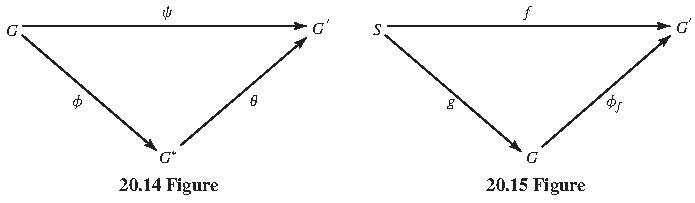
\includegraphics[width=0.953\linewidth,height=.8\textheight,keepaspectratio]{assets/p194_00.pdf}\end{center}
\end{BookFloat}

\BookExercise{13.}{Let \BookInline{S} be any set. A group \BookInline{G} together with a fixed function \BookInline{g:S\to G} constitutes a\textbf{ blop group on} \BookInline{S} if for each group \BookInline{G^{\prime }} and map \BookInline{f:S\to G^{\prime }} there exists a\textit{ unique} homomorphism \BookInline{\phi _{f}} of \BookInline{G} into \BookInline{G^{\prime }} such that \BookInline{f= \phi _{f}g(}see Fig. 20.15).}

\BookExercise{a.}{Let S be a fixed set. Show that if both \BookInline{G_{1},\allowbreak } together with \BookInline{g_{1}:S\to G_{1},\allowbreak } and \BookInline{G_{2},\allowbreak } together with \BookInline{g_{2}:S\to G_{2},\allowbreak } are blop groups on \BookInline{S,\allowbreak } then \BookInline{G_{1}} and \BookInline{G_{2}} are isomorphic. [\textit{Hint:} Show that \BookInline{g_{1}} and \BookInline{g_{2}} are one-to-one maps and that \BookInline{g_{1}S} and \BookInline{g_{2}S} generate \BookInline{G_{1}} and \BookInline{G_{2},\allowbreak } respectively. Then proceed in a way analogous to that given by the hint for Exercise 12.]}

\BookExercise{b.}{Let \BookInline{S} be a set. Show that a blop group on \BookInline{S} exists. You may use any theorems of the text.}

\BookExercise{c.}{What concept that we have introduced before corresponds to this idea of a blop group on \BookInline{S}?}

\BookExercise{14.}{Characterize a free abelian group by properties in a fashion similar to that used in Exercise 13.}

\end{BookBody}
\ifdefined\BookMaster\let\BookFinish\relax\else\def\BookFinish{\end{document}}\fi\BookFinish

\clearpage
% !TeX program = xelatex
\ifdefined\BookMaster\else
\documentclass[11pt,oneside]{article}
% !TeX program = xelatex
\usepackage[b5paper,left=22mm,right=22mm,top=20mm,bottom=22mm,footskip=11mm]{geometry}
\usepackage{fontspec}
\setmainfont{TeX Gyre Termes}
\setsansfont{TeX Gyre Heros}
\usepackage{amsmath,amssymb,mathtools,amsthm}
\renewcommand{\cdots}{\mathinner{\cdotp\cdotp\cdotp}}
\usepackage{graphicx,adjustbox,array,booktabs,longtable,multirow,enumitem,changepage,needspace}
\usepackage[table]{xcolor}
\usepackage{fancyhdr}
\raggedbottom
\interfootnotelinepenalty=10000
\newcommand{\BookFootnote}[2]{\begingroup\renewcommand{\thefootnote}{\fnsymbol{footnote}}\footnote[#1]{#2}\endgroup}
\newcommand{\BookFootnoteMark}[1]{\begingroup\renewcommand{\thefootnote}{\fnsymbol{footnote}}\footnotemark[#1]\endgroup}
\newcommand{\BookFootnoteText}[2]{\begingroup\renewcommand{\thefootnote}{\fnsymbol{footnote}}\footnotetext[#1]{#2}\endgroup}
\newenvironment{BookFloat}[1]{\par\addvspace{.6\baselineskip}\noindent\def\BookFloatID{#1}\begin{minipage}{\linewidth}\phantomsection\label{bookfloat:#1:start}}{\phantomsection\label{bookfloat:\BookFloatID:end}\end{minipage}\par\addvspace{.6\baselineskip}}

\usepackage[unicode,hidelinks]{hyperref}
\pagestyle{fancy}
\fancyhf{}
\newcommand{\BookFooter}{}
\fancyfoot[L]{\parbox[b]{\dimexpr\textwidth-15mm}{\footnotesize\BookFooter}}
\fancyfoot[R]{\footnotesize\thepage}
\renewcommand{\headrulewidth}{0pt}
\renewcommand{\footrulewidth}{0pt}
\setlength{\parindent}{0pt}
\setlength{\parskip}{0.2em}
\setlength{\emergencystretch}{3em}
\setlist{nosep,leftmargin=1.7em,labelsep=.65em}
\newif\ifBookNarrative
\BookNarrativetrue
\newenvironment{BookBody}{\setlength{\parindent}{0pt}}{}
\newcommand{\BookStatement}[1]{\par\addvspace{.6\baselineskip}\noindent #1\enspace\ignorespaces}
\newcommand{\BookLabel}[1]{\par\addvspace{.6\baselineskip}\needspace{3\baselineskip}\noindent\textbf{#1}\quad\ignorespaces}
\newcommand{\BookHeading}[1]{\par\addvspace{\baselineskip}\needspace{4\baselineskip}\noindent{\large\bfseries #1}\par\medskip}
\newcommand{\BookSubheading}[1]{\par\addvspace{.7\baselineskip}\needspace{3\baselineskip}\noindent{\bfseries #1}\par\smallskip}
\newcommand{\BookTextHeading}[1]{\par\addvspace{.7\baselineskip}\needspace{3\baselineskip}\noindent #1\par\smallskip}
\newcommand{\BookSectionTitle}[2]{\par\addvspace{1.2\baselineskip}\needspace{5\baselineskip}\noindent\colorbox{gray!25}{\sffamily\bfseries\small SECTION #1}\quad{\large\bfseries #2}\par\medskip}
\newcommand{\BookExerciseTitle}[1]{\par\addvspace{\baselineskip}\needspace{4\baselineskip}\noindent{\color{gray}\rule{1.5mm}{1.5mm}}\enspace{\large\bfseries Exercises #1}\par\medskip}
\newcommand{\BookBullet}[1]{\begin{list}{\textbullet}{\setlength{\leftmargin}{1.7em}\setlength{\labelwidth}{1em}\setlength{\labelsep}{.7em}\setlength{\topsep}{0pt}\setlength{\parsep}{0pt}\setlength{\itemsep}{0pt}}\item #1\end{list}}
\newcommand{\BookExercise}[2]{\begin{list}{\textbf{#1}}{\setlength{\leftmargin}{2.2em}\setlength{\labelwidth}{1.5em}\setlength{\labelsep}{.7em}\setlength{\topsep}{.15em}\setlength{\parsep}{0pt}\setlength{\itemsep}{0pt}}\item #2\end{list}}
\newcommand{\BookEnd}[1]{\unskip\nobreak\hfill\ensuremath{#1}}
\newcommand{\BookSource}[2]{\phantomsection\label{sourcepage:#1}} % Source-page anchors, retained through reflow.
\usepackage{multicol}
\usepackage{tikz}
\newcommand{\BookPartEntry}[2]{\par\noindent\makebox[17mm][l]{\bfseries Section #1}#2\par}
\newcommand{\BookPartTitle}[3]{\par\bigskip\noindent\begin{tikzpicture}\node[anchor=north west,inner sep=0pt,outer sep=0pt] (bookpart) at (0,0) {\begin{minipage}{\dimexpr\linewidth-.5pt}\hspace*{26mm}\begin{minipage}[t]{\dimexpr\linewidth-26mm}\begin{adjustbox}{max width=\linewidth}{\fontsize{20}{24}\selectfont\bfseries #2}\end{adjustbox}\par\vspace{6mm}\hrule\vspace{6mm}{\sffamily\footnotesize\setlength{\parskip}{.3em}#3}\vspace{3mm}\end{minipage}\end{minipage}};\path[shade,top color=gray!60,bottom color=white] (0,0) rectangle ([xshift=24mm]bookpart.south west);\node[anchor=north,font=\sffamily\bfseries\small] at (12mm,-2mm) {PART};\node[anchor=north,font=\sffamily\bfseries\Huge] at (12mm,-7mm) {#1};\end{tikzpicture}\par\bigskip}
\newsavebox{\BookMathBox}
\makeatletter
\newcommand{\BookInline}[1]{\leavevmode\hskip0pt\relax\begingroup\in@{\begin}{#1}\ifin@\sbox{\BookMathBox}{\(#1\)}\ifdim\wd\BookMathBox>\dimexpr\linewidth-1em\relax\resizebox{\dimexpr\linewidth-1em\relax}{!}{\usebox{\BookMathBox}}\else\(#1\)\fi\else\in@{\left}{#1}\ifin@\sbox{\BookMathBox}{\(#1\)}\ifdim\wd\BookMathBox>\dimexpr\linewidth-1em\relax\resizebox{\dimexpr\linewidth-1em\relax}{!}{\usebox{\BookMathBox}}\else\(#1\)\fi\else\(#1\)\fi\fi\endgroup\hskip0pt\relax}
\makeatother
\DeclareMathOperator{\Aut}{Aut}
\DeclareMathOperator{\End}{End}
\DeclareMathOperator{\Hom}{Hom}
\DeclareMathOperator{\GF}{GF}
\DeclareMathOperator{\irr}{irr}
\DeclareMathOperator{\lt}{lt}
\DeclareMathOperator{\lp}{lp}
\providecommand{\textcircled}[1]{\textnormal{(#1)}}

\begin{document}
\fi
\renewcommand{\BookFooter}{Section 21 Group Presentations}
\pdfbookmark[0]{Section 21 Group Presentations}{21_group_presentations}
\ifdefined\BookMaster\else\setcounter{page}{177}\fi
% Source PDF page 194; original printed page 177
\BookSource{194}{177}
\BookNarrativetrue

\begin{BookBody}

\BookSectionTitle{21}{Group Presentations}

\BookTextHeading{\textbf{Definition}}

\noindent Following most of the literature on group presentations, in this section we let 1 be the identity of a group. The idea of a\textit{ group presentation} is to form a group by giving a set of generators for the group and certain equations or relations that we want the generators to satisfy. We want the group to be as free as it possibly can be on the generators, subject to these relations.

\end{BookBody}

% Source PDF page 195; original printed page 178
\BookSource{195}{178}
\BookNarrativetrue

\begin{BookBody}

\BookLabel{21.1 Example} Suppose \BookInline{G} is\textit{ free with generation} \BookInline{x} \textit{and} \BookInline{y} \textit{except for the relation} \BookInline{xy= yx,\allowbreak } which we may express as \BookInline{xyx^{- 1}y^{- 1}= 1.} Note that the condition \BookInline{xy= yx} is exactly what is needed to make \BookInline{G} abelian, even though \BookInline{xyx^{- 1}y^{- 1}} is just one of the many possible commutators of \BookInline{F[\{x,\allowbreak y\}].} Thus \BookInline{G} is free abelian on two generators and is isomorphic to \BookInline{F[\{x,\allowbreak y\}]} modulo its commutator subgroup. This commutator subgroup of \BookInline{F[\{x,\allowbreak y\}]} is the smallest normal subgroup containing \BookInline{xyx^{- 1}y^{- 1},\allowbreak } since any normal subgroup containing \BookInline{xyx^{- 1}y^{- 1}} gives rise to a factor group that is abelian and thus contains the commutator subgroup by Theorem \BookInline{13.22.}\BookEnd{\blacktriangle}

The preceding example illustrates the general situation. Let \BookInline{F[A]} be a free group and suppose that we want to form a new group as much like \BookInline{F[A]} as it can be, subject to certain equations that we want satisfied. Any equation can be written in a form in which the right-hand side is 1. Thus we can consider the equations to be \BookInline{r_{i}= 1} for \BookInline{i\in I,\allowbreak } where \BookInline{r_{i}\in F[A].} If we require that \BookInline{r_{i}= 1,\allowbreak } then we will have to have

\begin{center}\begin{adjustbox}{max width=\linewidth}\BookInline{\displaystyle x\Big(r_{i}^{n}\Big)x^{- 1}= 1}\end{adjustbox}\end{center}

\noindent for any \BookInline{x\in F[A]} and \BookInline{n\in \mathbb{Z}.} Also any product of elements equal to 1 will again have to equal 1. Thus any finite product of the form

\begin{center}\begin{adjustbox}{max width=\linewidth}\BookInline{\displaystyle \prod _{j}x_{j}\Big(r_{i_{j}}^{n_{j}}\Big)x_{j}^{- 1},\allowbreak }\end{adjustbox}\end{center}

\noindent where the \BookInline{r_{i_{j}}} need not be distinct, will have to equal 1 in the new group. It is readily checked that the set of all these finite products is a normal subgroup \BookInline{R} of \BookInline{F[A].} Thus any group looking as much as possible like \BookInline{F[A],\allowbreak } subject to the requirements \BookInline{r_{i}= 1,\allowbreak } also has \BookInline{r= 1} for every \BookInline{r\in R.} But \BookInline{F[A]/R} looks like \BookInline{F[A](}remember that we multiply cosets by choosing representatives), except that \BookInline{R} has been collapsed to form the identity 1. Hence the group we are after is (at least isomorphic to\BookInline{)\; F[A]/R.} We can view this group as described by the generating set \BookInline{A} and the set \BookInline{\{r_{i}\mid i\in I\},\allowbreak } which we will abbreviate \BookInline{\{r_{i}\}.}

\BookTextHeading{\ensuremath{\blacksquare} \textbf{HISTORICAL NOTE}  }

\noindent The idea of a group presentation already appears in Arthur Cayley’s 1859 paper, “On the Theory of Groups as Depending on the Symbolic Equation \BookInline{\theta ^{n}= 1.} Third Part.” In this article, Cayley gives a complete enumeration of the five groups of order 8, both by listing all the elements of each and by giving for each a presentation. For example, his third example is what is here called the\textit{ dihedral group} \BookInline{D_{4};} Cayley notes that this group is generated by the two elements \BookInline{\alpha,\allowbreak \beta } with the relations \BookInline{\alpha ^{4}= 1,\allowbreak \beta ^{2}= 1,\allowbreak \alpha \beta = \beta \alpha ^{3}.} He also shows more generally that a group of order \BookInline{mn} is generated by \BookInline{\alpha,\allowbreak \beta } with the relations \BookInline{\alpha ^{m}= 1,\allowbreak } \BookInline{\beta ^{n}= 1,\allowbreak \alpha \beta = \beta \alpha ^{s}} if and only if \BookInline{s^{n}\equiv 1(}mod \BookInline{m)} (see Exercise 13).

\noindent In 1878, Cayley returned to the theory of groups and noted that a central problem in that theory is the determination of all groups of a given order \BookInline{n.} In the early 1890s, Otto Ho¨lder published several papers attempting to solve Cayley’s problem. Using techniques similar to those discussed in Sections 17 and 21, Ho¨lder determined all simple groups of order up to 200 and characterized all the groups of orders \BookInline{p^{3},\allowbreak pq^{2},\allowbreak pqr,\allowbreak } and \BookInline{p^{4},\allowbreak } where \BookInline{p,\allowbreak q,\allowbreak r} are distinct prime numbers. Furthermore, he developed techniques for determining the possible structures of a group \BookInline{G,\allowbreak } if one is given the structure of a normal subgroup \BookInline{H} and the structure of the factor group \BookInline{G/H.} Interestingly, since the notion of an abstract group was still fairly new at this time, Ho¨lder typically began his papers with the definition of a group and also emphasized that isomorphic groups are essentially one and the same object.

\BookLabel{21.2 Definition} Let \BookInline{A} be a set and let \BookInline{\{r_{i}\}\subseteq F[A].} Let \BookInline{R} be the least normal subgroup of \BookInline{F[A]} containing the \BookInline{r_{i}.} An isomorphism \BookInline{\phi } of \BookInline{F[A]/R} onto a group \BookInline{G} is a\textbf{ presentation of} \BookInline{G.} The 
% Source PDF page 196; original printed page 179
\BookSource{196}{179}
sets \BookInline{A} and \BookInline{\{r_{i}\}} give a\textbf{ group presentation.} The set \BookInline{A} is the set of\textbf{ generators for the} \textbf{presentation} and each \BookInline{r_{i}} is a\textbf{ relator.} Each \BookInline{r\in R} is a\textbf{ consequence of} \BookInline{\{r_{i}\}.} An equation \BookInline{r_{i}= 1} is a\textbf{ relation.} A\textbf{ finite presentation} is one in which both \BookInline{A} and \BookInline{\{r_{i}\}} are finite sets\BookInline{.}\BookEnd{\blacksquare}

\end{BookBody}

\BookNarrativetrue

\begin{BookBody}

This definition may seem complicated, but it really is not. In Example \BookInline{21.1,\allowbreak \{x,\allowbreak y\}} is our set of generators and \BookInline{xyx^{- 1}y^{- 1}} is the only relator. The equation \BookInline{xyx^{- 1}y^{- 1}= 1,\allowbreak } or \BookInline{xy= yx,\allowbreak } is a relation. This was an example of a finite presentation.

If a group presentation has generators \BookInline{x_{j}} and relators \BookInline{r_{i},\allowbreak } we shall use the notations

\begin{center}\begin{adjustbox}{max width=\linewidth}\BookInline{\displaystyle (x_{j}:r_{i})\;\text{or}\;(x_{j}:r_{i}= 1)}\end{adjustbox}\end{center}

\noindent to denote the group presentation. We may refer to \BookInline{F[\{x_{j}\}]/R} as\textit{ the group with presenta}\textit{tion} \BookInline{(x_{j}:r_{i}).}

\BookTextHeading{\textbf{Isomorphic Presentations}  }

\BookLabel{21.3 Example} Consider the group presentation with

\begin{center}\begin{adjustbox}{max width=\linewidth}\BookInline{\displaystyle A= \{a\}\;\text{and}\;\{r_{i}\}= \{a^{6}\},\allowbreak }\end{adjustbox}\end{center}

\noindent that is, the presentation

\begin{center}\begin{adjustbox}{max width=\linewidth}\BookInline{\displaystyle (a:a^{6}= 1).}\end{adjustbox}\end{center}

\noindent This group defined by one generator \BookInline{a,\allowbreak } with the relation \BookInline{a^{6}= 1,\allowbreak } is isomorphic to \BookInline{\mathbb{Z}_{6}.}

Now consider the group defined by two generators \BookInline{a} and \BookInline{b,\allowbreak } with \BookInline{a^{2}= 1,\allowbreak b^{3}= 1,\allowbreak } and \BookInline{ab= ba,\allowbreak } that is, the group with presentation

\begin{center}\begin{adjustbox}{max width=\linewidth}\BookInline{\displaystyle (a,\allowbreak b:a^{2},\allowbreak b^{3},\allowbreak aba^{- 1}b^{- 1}).}\end{adjustbox}\end{center}

\noindent The condition \BookInline{a^{2}= 1} gives \BookInline{a^{- 1}= a.} Also \BookInline{b^{3}= 1} gives \BookInline{b^{- 1}= b^{2}.} Thus every element in this group can be written as a product of nonnegative powers of \BookInline{a} and \BookInline{b.} The relation \BookInline{aba} \BookInline{^ { - 1 } b ^ { - 1 } = 1}, that is\BookInline{,\allowbreak ab= ba,\allowbreak } allows us to write first all the factors involving \BookInline{a} and then the factors involving \BookInline{b.} Hence every element of the group is equal to some \BookInline{a^{m}b^{n}.} But then \BookInline{a^{2}= 1} and \BookInline{b^{3}= 1} show that there are just six distinct elements,

\begin{center}\begin{adjustbox}{max width=\linewidth}\BookInline{\displaystyle 1,\allowbreak b,\allowbreak b^{2},\allowbreak a,\allowbreak ab,\allowbreak ab^{2}.}\end{adjustbox}\end{center}

\noindent The subgroup \BookInline{\langle ab\rangle } contains the elements \BookInline{1,\allowbreak ab,\allowbreak } and the powers of \BookInline{ab:}

\begin{center}\begin{adjustbox}{max width=\linewidth}\BookInline{\displaystyle \begin{aligned}(ab)^{2}&= a^{2}b^{2}= b^{2} \\ (ab)^{3}&= abb^{2}= a \\ (ab)^{4}&= a(ab)= b \\ (ab)^{5}&= (ab)b= ab^{2}.\end{aligned}}\end{adjustbox}\end{center}

\noindent So this group is also a cyclic group of order 6 isomorphic with \BookInline{\mathbb{Z}_{6}.} \BookEnd{\blacktriangle}

\BookLabel{21.4 Example} The dihedral group has presentation

\begin{center}\begin{adjustbox}{max width=\linewidth}\BookInline{\displaystyle D_{n}:(a,\allowbreak b|a^{n},\allowbreak b^{2},\allowbreak abab)}\end{adjustbox}\end{center}

\noindent since if we let \BookInline{a= \mu } and \BookInline{b= \rho } the three relations are exactly the defining relations for \BookInline{D_{n}.(}The last relation \BookInline{abab= 1} is equivalent to \BookInline{ab= ba^{- 1}.)} The element \BookInline{abab} is in \BookInline{R} if and only if \BookInline{b(abab)b^{- 1}} is in \BookInline{R} since \BookInline{R} is a normal subgroup. We have \BookInline{b(abab)b^{- 1}= } \BookInline{baba.} So in any presentation with generators \BookInline{a} and \BookInline{b} and a relator \BookInline{abab,\allowbreak } we can replace \BookInline{abab} with \BookInline{baba} and get the same subgroup \BookInline{R} and therefore the same factor group. Hence the dihedral group also has presentation

\begin{center}\begin{adjustbox}{max width=\linewidth}\BookInline{\displaystyle D_{n}:(a,\allowbreak b:a^{n},\allowbreak b^{2},\allowbreak baba).}\end{adjustbox}\end{center}

\end{BookBody}

% Source PDF page 197; original printed page 180
\BookSource{197}{180}
\BookNarrativetrue

\begin{BookBody}

\noindent Setting the relators to 1 gives the equivalent presentation

\begin{center}\begin{adjustbox}{max width=\linewidth}\BookInline{\displaystyle (a,\allowbreak b:a^{n}= 1,\allowbreak b^{2}= 1,\allowbreak ba= a^{- 1}b^{- 1})}\end{adjustbox}\end{center}

\noindent which can also be rewritten as

\begin{center}\begin{adjustbox}{max width=\linewidth}\BookInline{\displaystyle (a,\allowbreak b:a^{n}= 1,\allowbreak b^{2}= 1,\allowbreak ba= a^{n- 1}b).}\end{adjustbox}\end{center} \BookEnd{\blacktriangle}

The preceding examples illustrate that different presentations may give isomorphic groups. When this happens, we have\textbf{ isomorphic presentations.} To determine whether two presentations are isomorphic may be very hard. It has been shown (see Rabin [22]) that a number of such problems connected with this theory are not generally solvable; that is, there is no\textit{ routine} and well-defined way of discovering a solution in all cases. These unsolvable problems include the problem of deciding whether two presentations are isomorphic, whether a group given by a presentation is finite, free, abelian, or trivial, and the famous\textit{ word problem} of determining whether a given word \BookInline{w} is a consequence of a given set of relations \BookInline{\{r_{i}\}.}

The importance of this material is indicated by our Theorem 20.13, which guarantees that\textit{ every group has} \BookInline{a} \textit{presentation}.

\BookLabel{21.5 Example} Let us show that

\begin{center}\begin{adjustbox}{max width=\linewidth}\BookInline{\displaystyle (x,\allowbreak y:y^{2}x= y,\allowbreak yx^{2}y= x)}\end{adjustbox}\end{center}

\noindent is a presentation of the trivial group of one element. We need only show that \BookInline{x} and \BookInline{y} are consequences of the relators \BookInline{y^{2}xy^{- 1}} and \BookInline{yx^{2}yx^{- 1},\allowbreak } or that \BookInline{x= 1} and \BookInline{y= 1} can be deduced from \BookInline{y^{2}x= y} and \BookInline{yx^{2}y= x.} We illustrate both techniques.

As a consequence of \BookInline{y^{2}xy^{- 1},\allowbreak } we get \BookInline{yx} upon conjugation by \BookInline{y^{- 1}.} From \BookInline{yx} we deduce \BookInline{x^{- 1}y^{- 1},\allowbreak } and then \BookInline{(x^{- 1}y^{- 1})(yx^{2}yx^{- 1})} gives \BookInline{xyx^{- 1}.} Conjugating \BookInline{xyx^{- 1}} by \BookInline{x^{- 1},\allowbreak } we get \BookInline{y.} From \BookInline{y} we get \BookInline{y^{- 1},\allowbreak } and \BookInline{y^{- 1}(yx)} is \BookInline{x.}

Working with relations instead of relators, from \BookInline{y^{2}x= y} we deduce \BookInline{yx= 1} upon multiplication by \BookInline{y^{- 1}} on the left. Then substituting \BookInline{yx= 1} into \BookInline{yx^{2}y= x,\allowbreak } that is, \BookInline{(yx)(xy)= x,\allowbreak } we get \BookInline{xy= x.} Then multiplying by \BookInline{x^{- 1}} on the left, we have \BookInline{y= 1.} Substituting this in \BookInline{yx= 1,\allowbreak } we get \BookInline{x= 1.}

Both techniques amount to the same work, but it somehow seems more natural to most of us to work with relations\BookInline{.}\BookEnd{\blacktriangle}

\BookTextHeading{\textbf{Applications}}

\noindent We conclude this chapter with two applications.

\BookLabel{21.6 Example} Let us determine all groups of order 10 up to isomorphism. We know from the Fundamental Theorem 9.12 that every abelian group of order 10 is isomorphic to \BookInline{\mathbb{Z}_{10}.} Suppose that \BookInline{G} is nonabelian of order 10. By Sylow theory\BookInline{,\allowbreak G} contains a normal subgroup \BookInline{H} of order 5, and \BookInline{H} must be cyclic. Let \BookInline{a} be a generator of \BookInline{H.} Then \BookInline{G/H} is of order 2 and thus isomorphic to \BookInline{Z_{2}.} If \BookInline{b\in G} and \BookInline{b\notin H,\allowbreak } we must then have \BookInline{b^{2}\in H.} Since every element of \BookInline{H} except 1 has order 5, if \BookInline{b^{2}} were not equal to 1, then \BookInline{b^{2}} would have order 5, so \BookInline{b} would have order 10. This would mean that \BookInline{G} would be cyclic, contradicting our assumption that \BookInline{G} is not abelian. Thus \BookInline{b^{2}= 1.} Finally, since \BookInline{H} is a normal subgroup of \BookInline{G,\allowbreak bHb^{- 1}= H,\allowbreak } so in particular\BookInline{,\allowbreak bab^{- 1}\in H.} Since conjugation by \BookInline{b} is an automorphism of \BookInline{H,\allowbreak bab^{- 1}} must be another element of \BookInline{H} of order 5, hence \BookInline{bab^{- 1}} equals \BookInline{a,\allowbreak a^{2},\allowbreak a^{3},\allowbreak } or \BookInline{a^{4}.} But \BookInline{bab^{- 1}= a} would give \BookInline{ba= ab,\allowbreak } and then \BookInline{G} would be abelian, since \BookInline{a} and \BookInline{b} generate \BookInline{G.} Thus the possibilities for presentations of \BookInline{G} are:

\BookExercise{1.}{\BookInline{(a,\allowbreak b:a^{5}= 1,\allowbreak b^{2}= 1,\allowbreak ba= a^{2}b),\allowbreak }}

\BookExercise{2.}{\BookInline{(a,\allowbreak b:a^{5}= 1,\allowbreak b^{2}= 1,\allowbreak ba= a^{3}b),\allowbreak }}

\BookExercise{3.}{\BookInline{(a,\allowbreak b:a^{5}= 1,\allowbreak b^{2}= 1,\allowbreak ba= a^{4}b).}}

\end{BookBody}

% Source PDF page 198; original printed page 181
\BookSource{198}{181}
\BookNarrativetrue

\begin{BookBody}

Note that all three of these presentations can give groups of order at most 10, since the last relation \BookInline{ba= a^{i}b} enables us to express every product of \BookInline{a}’s and \BookInline{b}’s in \BookInline{G} in the form \BookInline{a^{s}b^{t}.} Then \BookInline{a^{5}= 1} and \BookInline{b^{2}= 1} show that the set

\begin{center}\begin{adjustbox}{max width=\linewidth}\BookInline{\displaystyle S= \{a^{0}b^{0},\allowbreak a^{1}b^{0},\allowbreak a^{2}b^{0},\allowbreak a^{3}b^{0},\allowbreak a^{4}b^{0},\allowbreak a^{0}b^{1},\allowbreak a^{1}b^{1},\allowbreak a^{2}b^{1},\allowbreak a^{3}b^{1},\allowbreak a^{4}b^{1}\}}\end{adjustbox}\end{center}

\noindent includes all elements of \BookInline{G.}

It is not yet clear that all these elements in \BookInline{S} are distinct, so that we have in all three cases a group of order 10. For example, the group presentation

\begin{center}\begin{adjustbox}{max width=\linewidth}\BookInline{\displaystyle (a,\allowbreak b:a^{5}= 1,\allowbreak b^{2}= 1,\allowbreak ba= a^{2}b)}\end{adjustbox}\end{center}

\noindent gives a group in which, using the associative law, we have

\begin{center}\begin{adjustbox}{max width=\linewidth}\BookInline{\displaystyle \begin{aligned}a&= b^{2}a= (bb)a= b(ba)= b(a^{2}b)= (ba)(ab) \\ &= (a^{2}b)(ab)= a^{2}(ba)b= a^{2}(a^{2}b)b= a^{4}b^{2}= a^{4}\end{aligned}}\end{adjustbox}\end{center}

\noindent Thus in this group\BookInline{,\allowbreak a= a^{4},\allowbreak } so \BookInline{a^{3}= 1,\allowbreak } which, together with \BookInline{a^{5}= 1,\allowbreak } yields \BookInline{a^{2}= 1.} But \BookInline{a^{2}= 1,\allowbreak } together with \BookInline{a^{3}= 1,\allowbreak } means that \BookInline{a= 1.} Hence every element in the group with presentation

\begin{center}\begin{adjustbox}{max width=\linewidth}\BookInline{\displaystyle (a,\allowbreak b:a^{5}= 1,\allowbreak b^{2}= 1,\allowbreak ba= a^{2}b)}\end{adjustbox}\end{center}

\noindent is equal to either 1 or \BookInline{b;} that is, this group is isomorphic to \BookInline{\mathbb{Z}_{2}.} A similar study of

\begin{center}\begin{adjustbox}{max width=\linewidth}\BookInline{\displaystyle (bb)a= b(ba)}\end{adjustbox}\end{center}

\noindent for

\begin{center}\begin{adjustbox}{max width=\linewidth}\BookInline{\displaystyle (a,\allowbreak b:a^{5}= 1,\allowbreak b^{2}= 1,\allowbreak ba= a^{3}b)}\end{adjustbox}\end{center}

\noindent shows that \BookInline{a= a^{4}} again, so this also yields a group isomorphic to \BookInline{\mathbb{Z}_{2}.}

This leaves just

\begin{center}\begin{adjustbox}{max width=\linewidth}\BookInline{\displaystyle (a,\allowbreak b:a^{5}= 1,\allowbreak b^{2}= 1,\allowbreak ba= a^{4}b)}\end{adjustbox}\end{center}

\noindent as a candidate for a nonabelian group of order 10. As in Example 21.4 this is a presentation of the dihedral group \BookInline{D_{5}.}

If we were unaware of the dihedral group, how would we show that the presentation gives a group with 10 elements? One attack is as follows. Let us try to make \BookInline{S} into a group by defining \BookInline{(a^{s}b^{t})(a^{u}b^{v})} to be \BookInline{a^{x}b^{y},\allowbreak } where \BookInline{x} is the remainder of \BookInline{s+ u(4^{t})} when divided by 5, and \BookInline{y} is the remainder of \BookInline{t+ v} when divided by 2, in the sense of the division algorithm (Theorem 6.2). The formula \BookInline{s+ u(4)^{t}} is counting what the power of \BookInline{a} should be after moving \BookInline{u} copies of \BookInline{a} by \BookInline{t} copies of \BookInline{b.} In other words, we use the relation \BookInline{ba= a^{4}b} as a guide in defining the product \BookInline{(a^{s}b^{t})(a^{u}b^{v})} of two elements of \BookInline{S.} We see that \BookInline{a^{0}b^{0}} acts as identity, and that given \BookInline{a^{u}b^{v},\allowbreak } we can determine \BookInline{t} and \BookInline{s} successively by letting

\begin{center}\begin{adjustbox}{max width=\linewidth}\BookInline{\displaystyle t\equiv - v(\;\text{mod}\;2)}\end{adjustbox}\end{center}

\noindent and then

\begin{center}\begin{adjustbox}{max width=\linewidth}\BookInline{\displaystyle s\equiv - u(4^{t})(\;\text{mod}\;5),\allowbreak }\end{adjustbox}\end{center}

\noindent giving \BookInline{a^{s}b^{t},\allowbreak } which is a left inverse for \BookInline{a^{u}b^{v}.} We will then have a group structure on \BookInline{S} if and only if the associative law holds. Exercise 13 asks us to carry out the straightforward computation for the associative law and to discover a condition for \BookInline{S} to be a group under such a definition of multiplication. The criterion of the exercise in this case amounts to the valid congruence

\begin{center}\begin{adjustbox}{max width=\linewidth}\BookInline{\displaystyle 4^{2}\equiv 1(\;\text{mod}\;5).}\end{adjustbox}\end{center}

\noindent Thus we do get a group of order 10. Note that

\begin{center}\begin{adjustbox}{max width=\linewidth}\BookInline{\displaystyle 2 ^ { 2 } \not \equiv 1 \left( \bmod 5 \right)}\end{adjustbox}\end{center}

\end{BookBody}

% Source PDF page 199; original printed page 182
\BookSource{199}{182}
\BookNarrativetrue

\begin{BookBody}

\noindent and

\begin{center}\begin{adjustbox}{max width=\linewidth}\BookInline{\displaystyle 3 ^ { 2 } \not \equiv 1 \pmod { 5 } ,\allowbreak }\end{adjustbox}\end{center}

\noindent so Exercise 13 also shows that

\begin{center}\begin{adjustbox}{max width=\linewidth}\BookInline{\displaystyle (a,\allowbreak b:a^{5}= 1,\allowbreak b^{2}= 1,\allowbreak ba= a^{2}b)}\end{adjustbox}\end{center}

\noindent and

\begin{center}\begin{adjustbox}{max width=\linewidth}\BookInline{\displaystyle (a,\allowbreak b:a^{5}= 1,\allowbreak b^{2}= 1,\allowbreak ba= a^{3}b)}\end{adjustbox}\end{center}

\noindent do not give groups of order 10. \BookEnd{\blacktriangle}

\BookLabel{21.7 Example} Let us determine all groups of order 8 up to isomorphism. We know the three abelian ones:

\begin{center}\begin{adjustbox}{max width=\linewidth}\BookInline{\displaystyle \mathbb{Z}_{8},\allowbreak \mathbb{Z}_{2}\times \mathbb{Z}_{4},\allowbreak \mathbb{Z}_{2}\times \mathbb{Z}_{2}\times \mathbb{Z}_{2}.}\end{adjustbox}\end{center}

\noindent Using generators and relations, we shall give presentations of the nonabelian groups.

Let \BookInline{G} be nonabelian of order 8. Since \BookInline{G} is nonabelian, it has no elements of order 8, so each element but the identity is of order either 2 or 4. If every element were of order 2, then for \BookInline{a,\allowbreak b\in G,\allowbreak } we would have \BookInline{(ab)^{2}= 1,\allowbreak } that is\BookInline{,\allowbreak abab= 1.} Then since \BookInline{a^{2}= 1} and \BookInline{b^{2}= 1} also, we would have

\begin{center}\begin{adjustbox}{max width=\linewidth}\BookInline{\displaystyle ba= a^{2}bab^{2}= a(ab)^{2}b= ab,\allowbreak }\end{adjustbox}\end{center}

\noindent contrary to our assumption that \BookInline{G} is not abelian. Thus \BookInline{G} must have an element of order 4.

Let \BookInline{\langle a\rangle } be a subgroup of \BookInline{G} of order 4. If \BookInline{b\notin \langle a\rangle,\allowbreak } the cosets \BookInline{\langle a\rangle } and \BookInline{b\langle a\rangle } exhaust all of \BookInline{G.} Hence \BookInline{a} and \BookInline{b} are generators for \BookInline{G} and \BookInline{a^{4}= 1.} Since \BookInline{\langle a\rangle } is normal in \BookInline{G(}by Sylow theory, or because it is of index \BookInline{2),\allowbreak G/\langle a\rangle } is isomorphic to \BookInline{\mathbb{Z}_{2}} and we have \BookInline{b^{2}\in \langle a\rangle.} If \BookInline{b^{2}= a} or \BookInline{b^{2}= a^{3},\allowbreak } then \BookInline{b} would be of order 8. Hence \BookInline{b^{2}= 1} or \BookInline{b^{2}= a^{2}.} Finally, since \BookInline{\langle a\rangle } is normal, we have \BookInline{bab^{- 1}\in \langle a\rangle,\allowbreak } and since \BookInline{b\langle a\rangle b^{- 1}} is a subgroup conjugate to \BookInline{\langle a\rangle } and hence isomorphic to \BookInline{\langle a\rangle,\allowbreak } we see that \BookInline{bab^{- 1}} must be an element of order 4. Thus \BookInline{bab^{- 1}= a} or \BookInline{bab^{- 1}= a^{3}.} If \BookInline{bab^{- 1}} were equal to \BookInline{a,\allowbreak } then \BookInline{ba} would equal \BookInline{ab,\allowbreak } which would make \BookInline{G} abelian. Hence \BookInline{bab^{- 1}= a^{3},\allowbreak } so \BookInline{ba= a^{3}b.} Thus we have two possibilities for \BookInline{G,\allowbreak } namely,

\begin{center}\begin{adjustbox}{max width=\linewidth}\BookInline{\displaystyle G_{1}:(a,\allowbreak b:a^{4}= 1,\allowbreak b^{2}= 1,\allowbreak ba= a^{3}b)}\end{adjustbox}\end{center}

\noindent and

\begin{center}\begin{adjustbox}{max width=\linewidth}\BookInline{\displaystyle G_{2}:(a,\allowbreak b:a^{4}= 1,\allowbreak b^{2}= a^{2},\allowbreak ba= a^{3}b).}\end{adjustbox}\end{center}

Note that \BookInline{a^{- 1}= a^{3},\allowbreak } and that \BookInline{b^{- 1}} is \BookInline{b} in \BookInline{G_{1}} and \BookInline{b^{3}} in \BookInline{G_{2}.} These facts, along with the relation \BookInline{ba= a^{3}b,\allowbreak } enable us to express every element in \BookInline{G_{i}} in the form \BookInline{a^{m}b^{n},\allowbreak } as in Examples 21.3 and 21.6. Since \BookInline{a^{4}= 1} and either \BookInline{b^{2}= 1} or \BookInline{b^{2}= a^{2},\allowbreak } the possible elements in each group are

\begin{center}\begin{adjustbox}{max width=\linewidth}\BookInline{\displaystyle 1,\allowbreak a,\allowbreak a^{2},\allowbreak a^{3},\allowbreak b,\allowbreak ab,\allowbreak a^{2}b,\allowbreak a^{3}b.}\end{adjustbox}\end{center}

\noindent Thus \BookInline{G_{1}} and \BookInline{G_{2}} each have order at most 8. The first group \BookInline{G_{1}} is sometimes called the \textbf{octic} group, but as we saw in Example 21.4 it is isomorphic with our old friend \BookInline{D_{4},\allowbreak } the dihedral group. For the second we can make \BookInline{S} into a group by defining \BookInline{(a^{i}b^{j})(a^{r}b^{s})} to be \BookInline{a^{x}b^{y}} where \BookInline{y} is \BookInline{j+ s} modulo 2 and if \BookInline{j+ s<2,\allowbreak } then \BookInline{x} is the remainder of \BookInline{i+ r(2j+ 1)} when divided by 4 and if \BookInline{j+ s= 2,\allowbreak } then \BookInline{x} is the remainder when \BookInline{i+ 2+ r(2j+ 1)} is divided by 4. We leave it as an exercise to show that this operation makes \BookInline{S} a group, which shows that \BookInline{G_{2}} is a presentation of a group of order 8.

Since \BookInline{ba= a^{3}b\neq ab,\allowbreak } we see that both \BookInline{G_{1}} and \BookInline{G_{2}} are nonabelian. That the two groups are not isomorphic follows from the fact that a computation shows that \BookInline{G_{1}} has only two elements of order 4, namely\BookInline{,\allowbreak a} and \BookInline{a^{3}.} On the other hand, in \BookInline{G_{2}} all elements but 1 and \BookInline{a^{2}} are of order 4. We leave the computations of the tables for these groups 
% Source PDF page 200; original printed page 183
\BookSource{200}{183}
to Exercise 3. To illustrate suppose we wish to compute \BookInline{(a^{2}b)(a^{3}b).} Using \BookInline{ba= a^{3}b} repeatedly, we get

\end{BookBody}

\BookNarrativetrue

\begin{BookBody}

\begin{center}\begin{adjustbox}{max width=\linewidth}\BookInline{\displaystyle (a^{2}b)(a^{3}b)= a^{2}(ba)a^{2}b= a^{5}(ba)ab= a^{8}(ba)b= a^{11}b^{2}.}\end{adjustbox}\end{center}

\noindent Then for \BookInline{G_{1},\allowbreak } we have

\begin{center}\begin{adjustbox}{max width=\linewidth}\BookInline{\displaystyle a^{11}b^{2}= a^{11}= a^{3},\allowbreak }\end{adjustbox}\end{center}

\noindent but if we are in \BookInline{G_{2},\allowbreak } we get

\begin{center}\begin{adjustbox}{max width=\linewidth}\BookInline{\displaystyle a^{11}b^{2}= a^{13}= a.}\end{adjustbox}\end{center}

The group \BookInline{G_{2}} is called the\textbf{ quaternion group}. We shall encounter the quaternion group again in Section \BookInline{32.}\BookEnd{\blacktriangle}

\end{BookBody}

\BookNarrativefalse

\begin{BookBody}

\BookExerciseTitle{21}

\BookTextHeading{\textbf{Computations}}

\BookExercise{1.}{Give a presentation of \BookInline{\mathbb{Z}_{4}} involving one generator; involving two generators; involving three generators.}

\BookExercise{2.}{Give a presentation of \BookInline{S_{3}} involving three generators.}

\BookExercise{3.}{Give the tables for both the octic group}

\begin{center}\begin{adjustbox}{max width=\linewidth}\BookInline{\displaystyle (a,\allowbreak b:a^{4}= 1,\allowbreak b^{2}= 1,\allowbreak ba= a^{3}b)}\end{adjustbox}\end{center}

\noindent and the quaternion group

\begin{center}\begin{adjustbox}{max width=\linewidth}\BookInline{\displaystyle (a,\allowbreak b:a^{4}= 1,\allowbreak b^{2}= a^{2},\allowbreak ba= a^{3}b).}\end{adjustbox}\end{center}

\noindent In both cases, write the elements in the order \BookInline{1,\allowbreak a,\allowbreak a^{2},\allowbreak a^{3},\allowbreak b,\allowbreak ab,\allowbreak a^{2}b,\allowbreak a^{3}b.(}Note that we do not have to compute\textit{ every} product. We know that these presentations give groups of order 8, and once we have computed enough products the rest are forced so that each row and each column of the table has each element exactly once.)

\BookExercise{4.}{Determine all groups of order 14 up to isomorphism. [\textit{Hint:} Follow the outline of Example 21.6 and use Exercise 13, part (b).]}

\BookExercise{5.}{Determine all groups of order 21 up to isomorphism. [\textit{Hint:} Follow the outline of Example 21.6 and use Exercise 13, part (b). It may seem that there are two presentations giving nonabelian groups. Show that they are isomorphic.]}

\BookTextHeading{\textbf{Concepts}}

\noindent In Exercises 6 and 7, correct the definition of the italicized term without reference to the text, if correction is needed, so that it is in a form acceptable for publication.

\BookExercise{6.}{A\textit{ consequence} of the set of relators is any finite product of relators raised to powers.}

\BookExercise{7.}{Two group presentations are\textit{ isomorphic} if and only if there is a one-to-one correspondence of the generators of the first presentation with the generators of the second that yields, by renaming generators, a one-to-one correspondence of the relators of the first presentation with those of the second.}

\BookExercise{8.}{Determine whether each of the following is true or false.}

\BookExercise{a.}{Every group has a presentation.}

\BookExercise{b.}{Every group has many different presentations.}

\BookExercise{c.}{Every group has two presentations that are not isomorphic.}

\BookExercise{d.}{Every group has a finite presentation.}

\BookExercise{e.}{Every group with a finite presentation is of finite order.}

\BookExercise{f.}{Every cyclic group has a presentation with just one generator.}

\BookExercise{g.}{Every conjugate of a relator is a consequence of the relator.}

\end{BookBody}

% Source PDF page 201; original printed page 184
\BookSource{201}{184}
\BookNarrativefalse

\begin{BookBody}

\BookExercise{h.}{Two presentations with the same number of generators are always isomorphic.}

\BookExercise{i.}{In a presentation of an abelian group, the set of consequences of the relators contains the commutator subgroup of the free group on the generators.}

\BookExercise{j.}{Every presentation of a free group has 1 as the only relator.}

\BookTextHeading{\textbf{Theory}}

\BookExercise{9.}{Use the methods of this section and Exercise 13, part (b), to show that there are no nonabelian groups of order 15.}

\BookExercise{10.}{Show, using Exercise 13, that}

\begin{center}\begin{adjustbox}{max width=\linewidth}\BookInline{\displaystyle (a,\allowbreak b:a^{3}= 1,\allowbreak b^{2}= 1,\allowbreak ba= a^{2}b)}\end{adjustbox}\end{center}

\noindent gives a group of order 6. Show that it is nonabelian.

\BookExercise{11.}{Show that the presentation}

\begin{center}\begin{adjustbox}{max width=\linewidth}\BookInline{\displaystyle (a,\allowbreak b:a^{3}= 1,\allowbreak b^{2}= 1,\allowbreak ba= a^{2}b)}\end{adjustbox}\end{center}

\noindent of Exercise 10 gives (up to isomorphism) the only nonabelian group of order 6, and hence gives a group isomorphic to \BookInline{S_{3}.}

\BookExercise{12.}{We showed in Example 13.6 that \BookInline{A_{4}} has no subgroup of order 6. The preceding exercise shows that such a subgroup of \BookInline{A_{4}} would have to be isomorphic to either \BookInline{\mathbb{Z}_{6}} or \BookInline{S_{3}.} Show again that this is impossible by considering orders of elements.}

\BookExercise{13.}{Let}

\begin{center}\begin{adjustbox}{max width=\linewidth}\BookInline{\displaystyle S= \{a^{i}b^{j}\mid 0\leq i<m,\allowbreak 0\leq j<n\},\allowbreak }\end{adjustbox}\end{center}

\noindent that is\BookInline{,\allowbreak S} consists of all formal products \BookInline{a^{i}b^{j}} starting with \BookInline{a^{0}b^{0}} and ending with \BookInline{a^{m- 1}b^{n- 1}.} Let \BookInline{r} be a positive integer, and define multiplication on \BookInline{S} by

\begin{center}\begin{adjustbox}{max width=\linewidth}\BookInline{\displaystyle (a^{s}b^{t})(a^{u}b^{v})= a^{x}b^{y},\allowbreak }\end{adjustbox}\end{center}

\noindent where \BookInline{x} is the remainder of \BookInline{s+ u(r^{t})} when divided by \BookInline{m,\allowbreak } and \BookInline{y} is the remainder of \BookInline{t+ v} when divided by \BookInline{n,\allowbreak } in the sense of the division algorithm (Theorem 6.2).

\BookExercise{a.}{Show that a necessary and sufficient condition for the associative law to hold and for \BookInline{S} to be a group under this multiplication is that \BookInline{r^{n}\equiv 1(}mod \BookInline{m).}}

\BookExercise{b.}{Deduce from part (a) that the group presentation}

\begin{center}\begin{adjustbox}{max width=\linewidth}\BookInline{\displaystyle (a,\allowbreak b:a^{m}= 1,\allowbreak b^{n}= 1,\allowbreak ba= a^{r}b)}\end{adjustbox}\end{center}

gives a group of order \BookInline{mn} if and only if \BookInline{r^{n}\equiv 1(}mod \BookInline{m).(}See the Historical Note in this section.)

\BookExercise{14.}{Without using Exercise 13, prove that \BookInline{(a,\allowbreak b:a^{5}= 1,\allowbreak b^{2}= 1,\allowbreak ba= a^{3}b)} is a presentation for the group \BookInline{\mathbb{Z}_{2}.}}

\BookExercise{15.}{Is the group obtained from the group presentation with the letters a through z as generators and the words in a standard English dictionary as relators the trivial group? Prove your answer.}

\end{BookBody}
\ifdefined\BookMaster\let\BookFinish\relax\else\def\BookFinish{\end{document}}\fi\BookFinish

\clearpage
% !TeX program = xelatex
\ifdefined\BookMaster\else
\documentclass[11pt,oneside]{article}
% !TeX program = xelatex
\usepackage[b5paper,left=22mm,right=22mm,top=20mm,bottom=22mm,footskip=11mm]{geometry}
\usepackage{fontspec}
\setmainfont{TeX Gyre Termes}
\setsansfont{TeX Gyre Heros}
\usepackage{amsmath,amssymb,mathtools,amsthm}
\renewcommand{\cdots}{\mathinner{\cdotp\cdotp\cdotp}}
\usepackage{graphicx,adjustbox,array,booktabs,longtable,multirow,enumitem,changepage,needspace}
\usepackage[table]{xcolor}
\usepackage{fancyhdr}
\raggedbottom
\interfootnotelinepenalty=10000
\newcommand{\BookFootnote}[2]{\begingroup\renewcommand{\thefootnote}{\fnsymbol{footnote}}\footnote[#1]{#2}\endgroup}
\newcommand{\BookFootnoteMark}[1]{\begingroup\renewcommand{\thefootnote}{\fnsymbol{footnote}}\footnotemark[#1]\endgroup}
\newcommand{\BookFootnoteText}[2]{\begingroup\renewcommand{\thefootnote}{\fnsymbol{footnote}}\footnotetext[#1]{#2}\endgroup}
\newenvironment{BookFloat}[1]{\par\addvspace{.6\baselineskip}\noindent\def\BookFloatID{#1}\begin{minipage}{\linewidth}\phantomsection\label{bookfloat:#1:start}}{\phantomsection\label{bookfloat:\BookFloatID:end}\end{minipage}\par\addvspace{.6\baselineskip}}

\usepackage[unicode,hidelinks]{hyperref}
\pagestyle{fancy}
\fancyhf{}
\newcommand{\BookFooter}{}
\fancyfoot[L]{\parbox[b]{\dimexpr\textwidth-15mm}{\footnotesize\BookFooter}}
\fancyfoot[R]{\footnotesize\thepage}
\renewcommand{\headrulewidth}{0pt}
\renewcommand{\footrulewidth}{0pt}
\setlength{\parindent}{0pt}
\setlength{\parskip}{0.2em}
\setlength{\emergencystretch}{3em}
\setlist{nosep,leftmargin=1.7em,labelsep=.65em}
\newif\ifBookNarrative
\BookNarrativetrue
\newenvironment{BookBody}{\setlength{\parindent}{0pt}}{}
\newcommand{\BookStatement}[1]{\par\addvspace{.6\baselineskip}\noindent #1\enspace\ignorespaces}
\newcommand{\BookLabel}[1]{\par\addvspace{.6\baselineskip}\needspace{3\baselineskip}\noindent\textbf{#1}\quad\ignorespaces}
\newcommand{\BookHeading}[1]{\par\addvspace{\baselineskip}\needspace{4\baselineskip}\noindent{\large\bfseries #1}\par\medskip}
\newcommand{\BookSubheading}[1]{\par\addvspace{.7\baselineskip}\needspace{3\baselineskip}\noindent{\bfseries #1}\par\smallskip}
\newcommand{\BookTextHeading}[1]{\par\addvspace{.7\baselineskip}\needspace{3\baselineskip}\noindent #1\par\smallskip}
\newcommand{\BookSectionTitle}[2]{\par\addvspace{1.2\baselineskip}\needspace{5\baselineskip}\noindent\colorbox{gray!25}{\sffamily\bfseries\small SECTION #1}\quad{\large\bfseries #2}\par\medskip}
\newcommand{\BookExerciseTitle}[1]{\par\addvspace{\baselineskip}\needspace{4\baselineskip}\noindent{\color{gray}\rule{1.5mm}{1.5mm}}\enspace{\large\bfseries Exercises #1}\par\medskip}
\newcommand{\BookBullet}[1]{\begin{list}{\textbullet}{\setlength{\leftmargin}{1.7em}\setlength{\labelwidth}{1em}\setlength{\labelsep}{.7em}\setlength{\topsep}{0pt}\setlength{\parsep}{0pt}\setlength{\itemsep}{0pt}}\item #1\end{list}}
\newcommand{\BookExercise}[2]{\begin{list}{\textbf{#1}}{\setlength{\leftmargin}{2.2em}\setlength{\labelwidth}{1.5em}\setlength{\labelsep}{.7em}\setlength{\topsep}{.15em}\setlength{\parsep}{0pt}\setlength{\itemsep}{0pt}}\item #2\end{list}}
\newcommand{\BookEnd}[1]{\unskip\nobreak\hfill\ensuremath{#1}}
\newcommand{\BookSource}[2]{\phantomsection\label{sourcepage:#1}} % Source-page anchors, retained through reflow.
\usepackage{multicol}
\usepackage{tikz}
\newcommand{\BookPartEntry}[2]{\par\noindent\makebox[17mm][l]{\bfseries Section #1}#2\par}
\newcommand{\BookPartTitle}[3]{\par\bigskip\noindent\begin{tikzpicture}\node[anchor=north west,inner sep=0pt,outer sep=0pt] (bookpart) at (0,0) {\begin{minipage}{\dimexpr\linewidth-.5pt}\hspace*{26mm}\begin{minipage}[t]{\dimexpr\linewidth-26mm}\begin{adjustbox}{max width=\linewidth}{\fontsize{20}{24}\selectfont\bfseries #2}\end{adjustbox}\par\vspace{6mm}\hrule\vspace{6mm}{\sffamily\footnotesize\setlength{\parskip}{.3em}#3}\vspace{3mm}\end{minipage}\end{minipage}};\path[shade,top color=gray!60,bottom color=white] (0,0) rectangle ([xshift=24mm]bookpart.south west);\node[anchor=north,font=\sffamily\bfseries\small] at (12mm,-2mm) {PART};\node[anchor=north,font=\sffamily\bfseries\Huge] at (12mm,-7mm) {#1};\end{tikzpicture}\par\bigskip}
\newsavebox{\BookMathBox}
\makeatletter
\newcommand{\BookInline}[1]{\leavevmode\hskip0pt\relax\begingroup\in@{\begin}{#1}\ifin@\sbox{\BookMathBox}{\(#1\)}\ifdim\wd\BookMathBox>\dimexpr\linewidth-1em\relax\resizebox{\dimexpr\linewidth-1em\relax}{!}{\usebox{\BookMathBox}}\else\(#1\)\fi\else\in@{\left}{#1}\ifin@\sbox{\BookMathBox}{\(#1\)}\ifdim\wd\BookMathBox>\dimexpr\linewidth-1em\relax\resizebox{\dimexpr\linewidth-1em\relax}{!}{\usebox{\BookMathBox}}\else\(#1\)\fi\else\(#1\)\fi\fi\endgroup\hskip0pt\relax}
\makeatother
\DeclareMathOperator{\Aut}{Aut}
\DeclareMathOperator{\End}{End}
\DeclareMathOperator{\Hom}{Hom}
\DeclareMathOperator{\GF}{GF}
\DeclareMathOperator{\irr}{irr}
\DeclareMathOperator{\lt}{lt}
\DeclareMathOperator{\lp}{lp}
\providecommand{\textcircled}[1]{\textnormal{(#1)}}

\begin{document}
\fi
\renewcommand{\BookFooter}{Section 22 Rings and Fields}
\pdfbookmark[0]{Section 22 Rings and Fields}{22_rings_and_fields}
\ifdefined\BookMaster\else\setcounter{page}{185}\fi
% Source PDF page 202; original printed page 185
\BookSource{202}{185}
\BookPartTitle{V}{Rings and Fields}{\BookPartEntry{22}{Rings and Fields}
\BookPartEntry{23}{Integral Domains}
\BookPartEntry{24}{Fermat’s and Euler’s Theorems}
\BookPartEntry{25}{Encryption}}

\BookNarrativetrue

\begin{BookBody}

\BookSectionTitle{22}{Rings and Fields}

\noindent All our work thus far has been concerned with sets on which a single binary operation has been defined. Our years of work with the integers and real numbers show that a study of sets on which two binary operations have been defined should be of great importance. Algebraic structures of this type are introduced in this section. In one sense, this section seems more intuitive than those that precede it, for the structures studied are closely related to those we have worked with for many years. However, we will be continuing with our axiomatic approach. So, from another viewpoint this study is more complicated than group theory, for we now have two binary operations and more axioms to deal with.

\BookTextHeading{\textbf{Definitions and Basic Properties}  }

\noindent The most general algebraic structure with two binary operations that we shall study is called a\textit{ ring}. As Example 22.2 following Definition 22.1 indicates, we have all worked with rings since elementary school.

\BookLabel{22.1 Definition} A\textbf{ ring} \BookInline{\langle R,\allowbreak +,\allowbreak \cdot \rangle } is a set \BookInline{R} together with two binary operations \BookInline{+ } and \BookInline{\cdot,\allowbreak } which we call \textit{addition} and\textit{ multiplication,} defined on \BookInline{R} such that the following axioms are satisfied:

\BookInline{\mathcal{R}_{1}.\langle R,\allowbreak + \rangle } is an abelian group.

\BookInline{\mathcal{R}_{2}.} Multiplication is associative.

\BookInline{\mathcal{R}_{3}.} For all \BookInline{a,\allowbreak b,\allowbreak c\in R,\allowbreak } the\textbf{ left distributive law}\BookInline{,\allowbreak a\cdot (b+ c)= (a\cdot b)+ (a\cdot c)} and the\textbf{ right distributive law} \BookInline{(a+ b)\cdot c= (a\cdot c)+ (b\cdot c)} hold\BookInline{.}\BookEnd{\blacksquare}

\BookLabel{22.2 Example} We are well aware that axioms \BookInline{\mathcal{R}_{1},\allowbreak \mathcal{R}_{2},\allowbreak } and \BookInline{\mathcal{R}_{3}} for a ring hold in any subset of the complex numbers that is a group under addition and that is closed under multiplication. For example\BookInline{,\allowbreak \langle \mathbb{Z},\allowbreak +,\allowbreak \cdot \rangle,\allowbreak \langle \mathbb{Q},\allowbreak +,\allowbreak \cdot \rangle,\allowbreak \langle \mathbb{R},\allowbreak +,\allowbreak \cdot \rangle,\allowbreak } and \BookInline{\langle \mathbb{C},\allowbreak +,\allowbreak \cdot \rangle } are rings\BookInline{.}\BookEnd{\blacktriangle}

\end{BookBody}

% Source PDF page 203; original printed page 186
\BookSource{203}{186}
\BookNarrativetrue

\begin{BookBody}

\BookTextHeading{\ensuremath{\blacksquare} \textbf{HISTORICAL NOTE}  }

\noindent The theory of rings grew out of the study of two particular classes of rings, polynomial rings in \BookInline{n} variables over the real or complex numbers (Section 27) and the “integers” of an algebraic number field. It was David Hilbert (1862–1943) who first introduced the term\textit{ ring,} in connection with the latter example, but it was not until the second decade of the twentieth century that a fully abstract definition appeared. The theory of commutative rings was given a firm axiomatic foundation by Emmy Noether (1882–1935) in her monumental paper “Ideal Theory in Rings,” which appeared in 1921. A major concept of this paper is the ascending chain condition for ideals. Noether proved that in any ring in which every ascending chain of ideals has a maximal element, every ideal is finitely generated.

Emmy Noether received her doctorate from the University of Erlangen, Germany, in 1907. Hilbert invited her to Go¨ttingen in 1915, but his efforts to secure her a paid position were blocked because of her sex. Hilbert complained, “I do not see that the sex of the candidate is an argument against her admission [to the faculty]. After all, we are a university, not a bathing establishment.” Noether was, however, able to lecture under Hilbert’s name. Ultimately, after the political changes accompanying the end of the First World War reached Go¨ttingen, she was given in 1923 a paid position at the University. For the next decade, she was very influential in the development of the basic concepts of modern algebra. Along with other Jewish faculty members, however, she was forced to leave Go¨ttingen in 1933. She spent the final two years of her life at Bryn Mawr College near Philadelphia.

It is customary to denote multiplication in a ring by juxtaposition, using \BookInline{ab} in place of \BookInline{a\cdot b.} We shall also observe the usual convention that multiplication is performed before addition in the absence of parentheses, so the left distributive law, for example, becomes

\begin{center}\begin{adjustbox}{max width=\linewidth}\BookInline{\displaystyle a(b+ c)= ab+ ac,\allowbreak }\end{adjustbox}\end{center}

\noindent without the parentheses on the right side of the equation. Also, as a convenience analogous to our notation in group theory, we shall somewhat incorrectly refer to a\textit{ ring} \BookInline{R} in place of a\textit{ ring} \BookInline{\langle R,\allowbreak +,\allowbreak \cdot \rangle,\allowbreak } provided that no confusion will result. In particular, from now on \BookInline{\mathbb{Z}} will always be \BookInline{\langle \mathbb{Z},\allowbreak +,\allowbreak \cdot \rangle,\allowbreak } and \BookInline{\mathbb{Q},\allowbreak \mathbb{R},\allowbreak } and \BookInline{\mathbb{C}} will also be the rings in Example 22.2. We may on occasion refer to \BookInline{\langle R,\allowbreak + \rangle } as\textit{ the additive group of the ring} \BookInline{R.}

\BookLabel{22.3 Example} Let \BookInline{R} be any ring and let \BookInline{M_{n}(R)} be the collection of all \BookInline{n\times n} matrices having elements of \BookInline{R} as entries. The operations of addition and multiplication in \BookInline{R} allow us to add and multiply matrices in the usual fashion, explained in the appendix. We can quickly check that \BookInline{\langle M_{n}(R),\allowbreak + \rangle } is an abelian group. The associativity of matrix multiplication and the two distributive laws in \BookInline{M_{n}(R)} are more tedious to demonstrate, but straightforward calculations indicate that they follow from the same properties in \BookInline{R.} We will assume from now on that we know that \BookInline{M_{n}(R)} is a ring. In particular, we have the rings \BookInline{M_{n}(\mathbb{Z}),\allowbreak M_{n}(\mathbb{Q}),\allowbreak M_{n}(\mathbb{R}),\allowbreak } and \BookInline{M_{n}(\mathbb{C}).} Note that multiplication is not a commutative operation in any of these rings for \BookInline{n\geq 2.}\BookEnd{\blacktriangle}

\BookLabel{22.4 Example} Let \BookInline{F} be the set of all functions \BookInline{f:\mathbb{R}\to \mathbb{R}.} We know that \BookInline{\langle F,\allowbreak + \rangle } is an abelian group under the usual function addition,

\begin{center}\begin{adjustbox}{max width=\linewidth}\BookInline{\displaystyle (f+ g)(x)= f(x)+ g(x).}\end{adjustbox}\end{center}

\noindent We define multiplication on \BookInline{F} by

\begin{center}\begin{adjustbox}{max width=\linewidth}\BookInline{\displaystyle (fg)(x)= f(x)g(x).}\end{adjustbox}\end{center}

\noindent That is\BookInline{,\allowbreak fg} is the function whose value at \BookInline{x} is \BookInline{f(x)g(x).} It is readily checked that \BookInline{F} is a ring; we leave the demonstration to Exercise 36. We have used this juxtaposition 
% Source PDF page 204; original printed page 187
\BookSource{204}{187}
notation \BookInline{\sigma \mu } for the composite function \BookInline{\sigma (\mu (x))} when discussing permutation multiplication. If we were to use both function multiplication and function composition in \BookInline{F,\allowbreak } we would use the notation \BookInline{f\circ g} for the composite function. However, we will use composition of functions almost exclusively with homomorphisms, which we will denote by Greek letters, and the usual product defined in this example chiefly when multiplying polynomial function’s \BookInline{f(x)g(x),\allowbreak } so no confusion should result\BookInline{.}\BookEnd{\blacktriangle}

\end{BookBody}

\BookNarrativetrue

\begin{BookBody}

\BookLabel{22.5 Example} Recall that in group theory\BookInline{,\allowbreak n\mathbb{Z}} is the cyclic subgroup of \BookInline{\mathbb{Z}} under addition consisting of all integer multiples of the integer \BookInline{n.} Since \BookInline{(nr)(ns)= n(nrs),\allowbreak } we see that \BookInline{n\mathbb{Z}} is closed under multiplication. The associative and distributive laws that hold in \BookInline{\mathbb{Z}} then assure us that \BookInline{\langle n\mathbb{Z},\allowbreak +,\allowbreak \cdot \rangle } is a ring. From now on in the text, we will consider \BookInline{n\mathbb{Z}} to be this ring\BookInline{.}\BookEnd{\blacktriangle}

\BookLabel{22.6 Example} Consider the cyclic group \BookInline{\langle \mathbb{Z}_{n},\allowbreak + \rangle.} If we define for \BookInline{a,\allowbreak b\in \mathbb{Z}_{n}} the product \BookInline{ab} as the remainder of the usual product of integers when divided by \BookInline{n,\allowbreak } it can be shown that \BookInline{\langle \mathbb{Z}_{n},\allowbreak +,\allowbreak \cdot \rangle } is a ring. We shall feel free to use this fact. For example, in \BookInline{\mathbb{Z}_{10}} we have \BookInline{(3)(7)= 1.} This operation on \BookInline{\mathbb{Z}_{n}} is\textbf{ multiplication modulo} \BookInline{n.} We do not check the ring axioms here, for they will follow in Section 30 from some of the theory we develop there. From now on\BookInline{,\allowbreak \mathbb{Z}_{n}} will always be the ring \BookInline{\langle \mathbb{Z}_{n},\allowbreak +,\allowbreak \cdot \rangle.}\BookEnd{\blacktriangle}

\BookLabel{22.7 Example} If \BookInline{R_{1},\allowbreak R_{2},\allowbreak \cdots,\allowbreak R_{n}} are rings, we can form the set \BookInline{R_{1}\times R_{2}\times \cdots \times R_{n}} of all ordered \BookInline{n-}tuples \BookInline{(r_{1},\allowbreak r_{2},\allowbreak \cdots,\allowbreak r_{n}),\allowbreak } where \BookInline{r_{i}\in R_{i}.} Defining addition and multiplication of \BookInline{n-}tuples by components (just as for groups), we see at once from the ring axioms in each component that the set of all these \BookInline{n-}tuples forms a ring under addition and multiplication by components. The ring \BookInline{R_{1}\times R_{2}\times \cdots \times R_{n}} is the\textbf{ direct product} of the rings \BookInline{R_{i}.}\BookEnd{\blacktriangle}

Continuing matters of notation, we shall always let 0 be the additive identity of a ring. The additive inverse of an element \BookInline{a} of a ring is \BookInline{- a.} We shall frequently have occasion to refer to a sum

\begin{center}\begin{adjustbox}{max width=\linewidth}\BookInline{\displaystyle a+ a+ \cdots + a}\end{adjustbox}\end{center}

\noindent having \BookInline{n} summands. We shall let this sum be \BookInline{n\cdot a,\allowbreak } always using the dot. However\BookInline{,\allowbreak n\cdot a} \textit{is not to be interpreted as} \BookInline{a} \textit{multiplication of} \BookInline{n} \textit{and} \BookInline{a} \textit{in the ring, for the integer} \BookInline{n} \textit{may} \textit{not be in the ring at all}. If \BookInline{n<0,\allowbreak } we let

\begin{center}\begin{adjustbox}{max width=\linewidth}\BookInline{\displaystyle n\cdot a= (- a)+ (- a)+ \cdots + (- a)}\end{adjustbox}\end{center}

\noindent for \BookInline{|n|} summands. Finally, we define

\begin{center}\begin{adjustbox}{max width=\linewidth}\BookInline{\displaystyle 0\cdot a= 0}\end{adjustbox}\end{center}

\noindent for \BookInline{0\in \mathbb{Z}} on the left side of the equations and \BookInline{0\in R} on the right side. Actually, the equation \BookInline{0a= 0} holds also for \BookInline{0\in R} on both sides. The following theorem proves this and various other elementary but important facts. Note the strong use of the distributive laws in the proof of this theorem. Axiom \BookInline{\mathcal{R}_{1}} for a ring concerns only addition, and axiom \BookInline{\mathcal{R}_{2}} concerns only multiplication. This shows that in order to prove anything that gives a relationship between these two operations, we are going to have to use axiom \BookInline{\mathcal{R}_{3}.} For example, the first thing that we will show in Theorem 22.8 is that \BookInline{0a= 0} for any element \BookInline{a} in a ring \BookInline{R.} Now this relation involves both addition and multiplication. The multiplication \BookInline{0a} stares us in the face, and 0 is an\textit{ additive} concept. Thus we will have to come up with an argument that uses a distributive law to prove this.

\BookLabel{22.8 Theorem} If \BookInline{R} is a ring with additive identity 0, then for any \BookInline{a,\allowbreak b\in R} we have

\BookExercise{1.}{\BookInline{0a= a0= 0,\allowbreak }}

\BookExercise{2.}{\BookInline{a(- b)= (- a)b= - (ab),\allowbreak }}

\BookExercise{3.}{\BookInline{(- a)(- b)= ab.}}

\end{BookBody}

% Source PDF page 205; original printed page 188
\BookSource{205}{188}
\BookNarrativetrue

\begin{BookBody}

\BookLabel{\textit{Proof}} For Property 1, note that by axioms \BookInline{\mathcal{R}_{1}} and \BookInline{\mathcal{R}_{2},\allowbreak }

\begin{center}\begin{adjustbox}{max width=\linewidth}\BookInline{\displaystyle a0+ a0= a(0+ 0)= a0= 0+ a0.}\end{adjustbox}\end{center}

\noindent Then by the cancellation law for the additive group \BookInline{\langle R,\allowbreak + \rangle,\allowbreak } we have \BookInline{a0= 0.} Likewise,

\begin{center}\begin{adjustbox}{max width=\linewidth}\BookInline{\displaystyle 0a+ 0a= (0+ 0)a= 0a= 0+ 0a}\end{adjustbox}\end{center}

\noindent implies that \BookInline{0a= 0.} This proves Property 1.

In order to understand the proof of Property 2, we must remember that, by \textit{definition}\BookInline{,\allowbreak - (ab)} is the element that when added to \BookInline{ab} gives 0. Thus to show that \BookInline{a(- b)= - (ab),\allowbreak } we must show precisely that \BookInline{a(- b)+ ab= 0.} By the left distributive law,

\begin{center}\begin{adjustbox}{max width=\linewidth}\BookInline{\displaystyle a(- b)+ ab= a(- b+ b)= a0= 0,\allowbreak }\end{adjustbox}\end{center}

\noindent since a\BookInline{0= 0} by Property 1. Likewise,

\begin{center}\begin{adjustbox}{max width=\linewidth}\BookInline{\displaystyle (- a)b+ ab= (- a+ a)b= 0b= 0.}\end{adjustbox}\end{center}

\noindent For Property 3, note that

\begin{center}\begin{adjustbox}{max width=\linewidth}\BookInline{\displaystyle (- a)(- b)= - (a(- b))}\end{adjustbox}\end{center}

\noindent by Property 2. Again by Property 2,

\begin{center}\begin{adjustbox}{max width=\linewidth}\BookInline{\displaystyle - (a(- b))= - (- (ab)),\allowbreak }\end{adjustbox}\end{center}

\noindent and \BookInline{- (- (ab))} is the element that when added to \BookInline{- (ab)} gives 0. This is \BookInline{ab} by definition of \BookInline{- (ab)} and by the uniqueness of an inverse in a group. Thus\BookInline{,\allowbreak (- a)(- b)= ab.}\BookEnd{\blacklozenge}

Based on high school algebra it seems natural to begin a proof of Property 2 in Theorem 22.8 by writing \BookInline{(- a)b= ((- 1)a)b.} In Exercise 30 you will be asked to find an error in a “proof” of this sort.

It is important that you\textit{ understand} the preceding proof. The theorem allows us to use our usual rules for signs.

\BookTextHeading{\textbf{Homomorphisms and Isomorphisms}  }

\noindent From our work in group theory, it is quite clear how a structure-relating map of a ring \BookInline{R} into a ring \BookInline{R^{\prime }} should be defined.

\BookLabel{22.9 Definition} For rings \BookInline{R} and \BookInline{R^{\prime },\allowbreak } a map \BookInline{\phi:R\to R^{\prime }} is a\textbf{ homomorphism} if the following two conditions are satisfied for all \BookInline{a,\allowbreak b\in R:}

\BookExercise{1.}{\BookInline{\phi (a+ b)= \phi (a)+ \phi (b),\allowbreak }}

\BookExercise{2.}{\BookInline{\phi (ab)= \phi (a)\phi (b).}} \BookEnd{\blacksquare}

In the preceding definition, Condition 1 is the statement that \BookInline{\phi } is a group homomorphism mapping the abelian group \BookInline{\langle R,\allowbreak + \rangle } into \BookInline{\langle R^{\prime },\allowbreak + \rangle.} Condition 2 requires that \BookInline{\phi } relate the multiplicative structures of the rings \BookInline{R} and \BookInline{R^{\prime }} in the same way. Since \BookInline{\phi } is also a group homomorphism, all the results concerning group homomorphisms are valid for the additive structure of the rings. In particular\BookInline{,\allowbreak \phi } is one-to-one if and only if its\textbf{ kernel} Ker\BookInline{(\phi )= \{a\in R\mid \phi (a)= 0^{\prime }\}} is just the subset \BookInline{\{0\}} of \BookInline{R.} The homomorphism \BookInline{\phi } of the group \BookInline{\langle R,\allowbreak + \rangle } gives rise to a factor group. We expect that a ring homomorphism will give rise to a factor ring. This is indeed the case. We delay discussion of this to Section 30, where the treatment will parallel our treatment of factor groups in Section 12.

\end{BookBody}

% Source PDF page 206; original printed page 189
\BookSource{206}{189}
\BookNarrativetrue

\begin{BookBody}

\BookLabel{22.10 Example} Let \BookInline{F} be the ring of all functions mapping \BookInline{\mathbb{R}} into \BookInline{\mathbb{R}} defined in Example 22.4. For each \BookInline{a\in \mathbb{R},\allowbreak } we have the\textbf{ evaluation homomorphism} \BookInline{\phi _{a}:F\to \mathbb{R},\allowbreak } where \BookInline{\phi _{a}(f)= f(a)} for \BookInline{f\in F.} We will work a great deal with this homomorphism in the rest of this text, for finding a real solution of a polynomial equation \BookInline{p(x)= 0} amounts precisely to finding \BookInline{a\in \mathbb{R}} such that \BookInline{\phi _{a}(p)= 0.} Much of the remainder of this text deals with solving polynomial equations. We leave the demonstration of the homomorphism properties for \BookInline{\phi _{a}} to Exercise \BookInline{37.}\BookEnd{\blacktriangle}

\BookLabel{22.11 Example} The map \BookInline{\phi:\mathbb{Z}\to \mathbb{Z}_{n}} where \BookInline{\phi (a)} is the remainder of \BookInline{a} modulo \BookInline{n} is a ring homomorphism for each positive integer \BookInline{n.} We know \BookInline{\phi (a+ b)= \phi (a)+ \phi (b)} by group theory. To show the multiplicative property, write \BookInline{a= q_{1}n+ r_{1}} and \BookInline{b= q_{2}n+ r_{2}} according to the division algorithm. Then \BookInline{ab= n(q_{1}q_{2}n+ r_{1}q_{2}+ q_{1}r_{2})+ r_{1}r_{2}.} Thus \BookInline{\phi (ab)} is the remainder of \BookInline{r_{1}r_{2}} when divided by \BookInline{n.} Since \BookInline{\phi (a)= r_{1}} and \BookInline{\phi (b)= r_{2},\allowbreak } Example 22.6 indicates that \BookInline{\phi (a)\phi (b)} is also this same remainder, so \BookInline{\phi (ab)= \phi (a)\phi (b).} From group theory, we anticipate that the ring \BookInline{\mathbb{Z}_{n}} might be isomorphic to a factor ring \BookInline{\mathbb{Z}/n\mathbb{Z}.} This is indeed the case; factor rings will be discussed in Section \BookInline{30.}\BookEnd{\blacktriangle}

We realize that in the study of any sort of mathematical structure, an idea of basic importance is the concept of two systems being\textit{ structurally identical}, that is, one being just like the other except for names. In algebra this concept is always called\textit{ isomor}\textit{phism}. The concept of two things being just alike except for names of elements leads us, just as it did for groups, to the following definition.

\BookLabel{22.12 Definition} An\textbf{ isomorphism} \BookInline{\phi:R\to R^{\prime }} from a ring \BookInline{R} to a ring \BookInline{R^{\prime }} is a homomorphism that is one-to-one and onto \BookInline{R^{\prime }.} The rings \BookInline{R} and \BookInline{R^{\prime }} are then\textbf{ isomorphic}\BookInline{.}\BookEnd{\blacksquare}

From our work in group theory, we expect that isomorphism gives an equivalence relation on any collection of rings. We need to check that the multiplicative property of an isomorphism is satisfied for the inverse map \BookInline{\phi ^{- 1}:R^{\prime }\to R(}to complete the symmetry argument). Similarly, we check that if \BookInline{\mu:R^{\prime }\to R^{\prime \prime }} is also a ring isomorphism, then the multiplicative requirement holds for the composite map \BookInline{\mu \phi:R\to R^{\prime \prime }(}to complete the transitivity argument). We ask you to do this in Exercise 38.

\BookLabel{22.13 Example} As abelian groups\BookInline{,\allowbreak \langle \mathbb{Z},\allowbreak + \rangle } and \BookInline{\langle 2\mathbb{Z},\allowbreak + \rangle } are isomorphic under the map \BookInline{\phi:\mathbb{Z}\to 2\mathbb{Z},\allowbreak } with \BookInline{\phi (x)= 2x} for \BookInline{x\in \mathbb{Z}.} Here \BookInline{\phi } is\textit{ not} a ring isomorphism, for \BookInline{\phi (xy)= 2xy,\allowbreak } while \BookInline{\phi (x)\phi (y)= 2x2y= 4xy.}\BookEnd{\blacktriangle}

\BookTextHeading{\textbf{Multiplicative Questions: Fields}  }

\noindent Many of the rings we have mentioned, such as \BookInline{\mathbb{Z},\allowbreak \mathbb{Q},\allowbreak } and \BookInline{\mathbb{R},\allowbreak } have a multiplicative identity element 1. However\BookInline{,\allowbreak 2\mathbb{Z}} does not have an identity element for multiplication. Note also that multiplication is not commutative in the matrix rings described in Example 22.3.

It is evident that \BookInline{\{0\},\allowbreak } with \BookInline{0+ 0= 0} and \BookInline{(0)(0)= 0,\allowbreak } gives a ring, the\textbf{ zero ring.} Here 0 acts as multiplicative as well as additive identity element. By Theorem 22.8, this is the only case in which 0 could act as a multiplicative identity element, for from \BookInline{0a= 0,\allowbreak } we can then deduce that \BookInline{a= 0.} Theorem 1.15 shows that if a ring has a multiplicative identity element, it is unique. We denote a multiplicative identity element in a ring by 1.

\BookLabel{22.14 Definition} A ring in which the multiplication is commutative is a\textbf{ commutative ring.} A ring with a multiplicative identity element is a\textbf{ ring with unity;} the multiplicative identity element 1 is called “\textbf{unity.}” \BookEnd{\blacksquare}

\end{BookBody}

% Source PDF page 207; original printed page 190
\BookSource{207}{190}
\BookNarrativetrue

\begin{BookBody}

\noindent In a ring with unity 1 the distributive laws show that

\begin{center}\begin{adjustbox}{max width=\linewidth}\BookInline{\displaystyle \begin{aligned}(1+ 1+ \cdots + 1)(1+ 1+ \cdots + 1)&= (1+ 1+ \cdots + 1),\allowbreak  \\ &n\;\text{summands}\;m\;\text{summands}\;nm\;\text{summands}\;\end{aligned}}\end{adjustbox}\end{center}

\noindent that is\BookInline{,\allowbreak (n\cdot 1)(m\cdot 1)= (nm)\cdot 1.} The next example gives an application of this observation.

\BookLabel{22.15 Example} We claim that for integers \BookInline{r} and \BookInline{s} where gcd\BookInline{(r,\allowbreak s)= 1,\allowbreak } the rings \BookInline{\mathbb{Z}_{rs}} and \BookInline{\mathbb{Z}_{r}\times \mathbb{Z}_{s}} are isomorphic. Additively, they are both cyclic abelian groups of order \BookInline{rs} with generators 1 and (1, 1) respectively. Thus \BookInline{\phi:\mathbb{Z}_{rs}\to \mathbb{Z}_{r}\times \mathbb{Z}_{s}} defined by \BookInline{\phi (n\cdot 1)= n\cdot (1,\allowbreak 1)} is an additive group isomorphism. To check the multiplicative Condition 2 of Definition 22.9, we use the observation preceding this example for the unity (1, 1) in the ring \BookInline{\mathbb{Z}_{r}\times \mathbb{Z}_{s},\allowbreak } and compute.

\begin{center}\begin{adjustbox}{max width=\linewidth}\BookInline{\displaystyle \phi (nm)= (nm)\cdot (1,\allowbreak 1)= [n\cdot (1,\allowbreak 1)][m\cdot (1,\allowbreak 1)]= \phi (n)\phi (m).}\end{adjustbox}\end{center} \BookEnd{\blacktriangle}

Note that a direct product \BookInline{R= R_{1}\times R_{2}\times \cdots \times R_{n}} of rings is commutative if and and only if each ring \BookInline{R_{i}} is commutative. Furthermore\BookInline{,\allowbreak R} has a unity if and only if each \BookInline{R_{i}} has a unity.

The set \BookInline{\mathbb{R}^{\ast }} of nonzero real numbers forms a group under multiplication. However, the nonzero integers do not form a group under multiplication since only the integers 1 and \BookInline{- 1} have multiplicative inverses in \BookInline{\mathbb{Z}.} In general, a\textbf{ multiplicative inverse} of an element \BookInline{a} in a ring \BookInline{R} with unity \BookInline{1\neq 0} is an element \BookInline{a^{- 1}\in R} such that \BookInline{aa^{- 1}= a^{- 1}a= 1.} Precisely as for groups, a multiplicative inverse for an element \BookInline{a} in \BookInline{R} is unique, if it exists at all (see Exercise 45). Theorem 22.8 shows that it would be hopeless to have a multiplicative inverse for 0 except for the ring \BookInline{\{0\},\allowbreak } where \BookInline{0+ 0= 0} and \BookInline{(0)(0)= 0,\allowbreak } with 0 as both additive and multiplicative identity element. We are thus led to discuss the existence of multiplicative inverses for nonzero elements in a ring with nonzero unity. There is unavoidably a lot of terminology to be defined in this introductory section on rings. We are almost done.

\BookLabel{22.16 Definition} Let \BookInline{R} be a ring with unity \BookInline{1\neq 0.} An element \BookInline{u} in \BookInline{R} is a\textbf{ unit} of \BookInline{R} if it has a multiplicative inverse in \BookInline{R.} If every nonzero element of \BookInline{R} is a unit, then \BookInline{R} is a\textbf{ division ring} (or\textbf{ skew} \textbf{field}). A\textbf{ field} is a commutative division ring. A noncommutative division ring is called a “\textbf{strictly skew field.}” \BookEnd{\blacksquare}

\BookLabel{22.17 Example} Let us find the units in \BookInline{\mathbb{Z}_{14}.} Of course, 1 and \BookInline{- 1= 13} are units. Since \BookInline{(3)(5)= 1} we see that 3 and 5 are units; therefore \BookInline{- 3= 11} and \BookInline{- 5= 9} are also units. None of the remaining elements of \BookInline{\mathbb{Z}_{14}} can be units, since no multiple of 2, 4, 6, 7, 8, or 10 can be one more than a multiple of 14; they all have a common factor, either 2 or 7, with 14. Section 24 will show that the units in \BookInline{\mathbb{Z}_{n}} are precisely those \BookInline{m\in \mathbb{Z}_{n}} such that gcd \BookInline{(m,\allowbreak n)= 1.}\BookEnd{\blacktriangle}

\BookLabel{22.18 Example} \BookInline{\mathbb{Z}} is not a field, because 2, for example, has no multiplicative inverse, so 2 is not a unit in \BookInline{\mathbb{Z}.} The only units in \BookInline{\mathbb{Z}} are 1 and \BookInline{- 1.} However\BookInline{,\allowbreak \mathbb{Q}} and \BookInline{\mathbb{R}} are fields. An example of a strictly skew field is given in Section \BookInline{32.}\BookEnd{\blacktriangle}

We have the natural concepts of a subring of a ring and a subfield of a field. A \textbf{subring of a ring} is a subset of the ring that is a ring under induced operations from the whole ring; a\textbf{ subfield} is defined similarly for a subset of a field. In fact, let us say here once and for all that if we have a set, together with a certain specified type of\textit{ algebraic} \textit{structure} (group, ring, field, integral domain, vector space, and so on), then any subset of this set, together with a natural induced algebraic structure\textit{ that yields an algebraic} \textit{structure of the same type}, is a\textit{ substructure}. If \BookInline{K} and \BookInline{L} are both structures, we shall let \BookInline{K\leq L} denote that \BookInline{K} is a substructure of \BookInline{L} and \BookInline{K<L} denote that \BookInline{K\leq L} but \BookInline{K\neq L.} Exercise 50 gives criteria for a subset \BookInline{S} of a ring \BookInline{R} to form a subring of \BookInline{R.}

\end{BookBody}

% Source PDF page 208; original printed page 191
\BookSource{208}{191}
\BookNarrativetrue

\begin{BookBody}

\BookTextHeading{\textbf{HISTORICAL NOTE}  } \BookEnd{\blacksquare}

\noindent Although fields were implict in the early work on the solvability of equations by Abel and Galois, it was Leopold Kronecker (1823– 1891) who in connection with his own work on this subject first published in 1881 a definition of what he called a “domain of rationality”: “The domain of rationality \BookInline{(R^{\prime },\allowbreak R^{\prime \prime },\allowbreak R^{\prime \prime \prime },\allowbreak \cdots )} contains \BookInline{\cdots } every one of those quantities which are rational functions of the quantities \BookInline{R^{\prime },\allowbreak R^{\prime \prime },\allowbreak R^{\prime \prime \prime },\allowbreak \cdots } with integral coefficients.” Kronecker, however, who insisted that any mathematical subject must be constructible in finitely many steps, did not view the domain of rationality as a complete entity, but merely as a region in which took place various operations on its elements.

\noindent Richard Dedekind (1831–1916), the inventor of the Dedekind cut definition of a real number, considered a field as a completed entity. In 1871, he published the following definition in his supplement to the second edition of Dirichlet’s text on number theory: “By a field we mean any system of infinitely many real or complex numbers, which in itself is so closed and complete, that the addition, subtraction, multiplication, and division of any two numbers always produces a number of the same system.” Both Kronecker and Dedekind had, however, dealt with their varying ideas of this notion as early as the 1850s in their university lectures.

A more abstract definition of a field, similar to the one in the text, was given by Heinrich Weber (1842–1913) in a paper of 1893. Weber’s definition, unlike that of Dedekind, specifically included fields with finitely many elements as well as other fields, such as function fields, which were not subfields of the field of complex numbers.

Finally, be careful not to confuse our use of the words\textit{ unit} and\textit{ unity}.\textit{ Unity} is the multiplicative identity element, while a\textit{ unit} is any element having a multiplicative inverse. Thus the multiplicative identity element or unity is a unit, but not every unit is unity. For example\BookInline{,\allowbreak - 1} is a unit in \BookInline{\mathbb{Z},\allowbreak } but \BookInline{- 1} is not unity, that is\BookInline{,\allowbreak - 1\neq 1.}

\end{BookBody}

\BookNarrativefalse

\begin{BookBody}

\BookExerciseTitle{22}

\BookTextHeading{\textbf{Computations}}

\noindent In Exercises 1 through 6, compute the product in the given ring.

\BookExercise{1.}{(12)(16) in \BookInline{\mathbb{Z}_{24}}}

\BookExercise{2.}{(16)(3) in \BookInline{\mathbb{Z}_{32}}}

\BookExercise{3.}{\BookInline{(11)(- 4)} in \BookInline{\mathbb{Z}_{15}}}

\BookExercise{4.}{\BookInline{(20)(- 8)} in \BookInline{\mathbb{Z}_{26}}}

\BookExercise{5.}{(2,3)(3,5) in \BookInline{\mathbb{Z}_{5}\times \mathbb{Z}_{9}}}

\BookExercise{6.}{\BookInline{(- 3,\allowbreak 5)(2,\allowbreak - 4)} in \BookInline{\mathbb{Z}_{4}\times \mathbb{Z}_{11}}}

\noindent In Exercises 7 through 13, decide whether the indicated operations of addition and multiplication are defined (closed) on the set, and give a ring structure. If a ring is not formed, tell why this is the case. If a ring is formed, state whether the ring is commutative, whether it has unity, and whether it is a field.

\BookExercise{7.}{\BookInline{n\mathbb{Z}} with the usual addition and multiplication}

\BookExercise{8.}{\BookInline{\mathbb{Z}^{+ }} with the usual addition and multiplication}

\BookExercise{9.}{\BookInline{\mathbb{Z}\times \mathbb{Z}} with addition and multiplication by components}

\BookExercise{10.}{\BookInline{2\mathbb{Z}\times \mathbb{Z}} with addition and multiplication by components}

\BookExercise{11.}{\BookInline{\{a+ b\sqrt{2}\mid a,\allowbreak b\in \mathbb{Z}\}} with the usual addition and multiplication}

\BookExercise{12.}{\BookInline{\{a+ b\sqrt{2}\mid a,\allowbreak b\in \mathbb{Q}\}} with the usual addition and multiplication}

\BookExercise{13.}{The set of all pure imaginary complex numbers\textit{ ri} for \BookInline{r\in \mathbb{R}} with the usual addition and multiplication}

\end{BookBody}

% Source PDF page 209; original printed page 192
\BookSource{209}{192}
\BookNarrativefalse

\begin{BookBody}

\noindent In Exercises 14 through 19, describe all units in the given ring

\BookExercise{14.}{\BookInline{\mathbb{Z}}}

\BookExercise{15.}{\BookInline{\mathbb{Z}\times \mathbb{Z}}}

\BookExercise{16.}{\BookInline{\mathbb{Z}_{5}}}

\BookExercise{17.}{\BookInline{\mathbb{Q}}}

\BookExercise{18.}{\BookInline{\mathbb{Z}\times \mathbb{Q}\times \mathbb{Z}}}

\BookExercise{19.}{\BookInline{\mathbb{Z}_{4}}}

\BookExercise{20.}{Consider the matrix ring \BookInline{M_{2}(\mathbb{Z}_{2}).} \textbf{a.} Find the\textbf{ order} of the ring, that is, the number of elements in it. \textbf{b.} List all units in the ring.}

\BookExercise{21.}{If possible, give an example of a homomorphism \BookInline{\phi:R\to R^{\prime }} where \BookInline{R} and \BookInline{R^{\prime }} are rings with unity \BookInline{1\neq 0} and \BookInline{1 ^ { \prime } \neq 0 ^ { \prime }}, and where \BookInline{\phi (1)\neq 0^{\prime }} and \BookInline{\phi (1)\neq 1^{\prime }.}}

\BookExercise{22.}{(Linear algebra) Consider the map det of \BookInline{M_{n}(\mathbb{R})} into \BookInline{\mathbb{R}} where det\BookInline{(A)} is the determinant of the matrix \BookInline{A} for \BookInline{A\in M_{n}(\mathbb{R}).} Is det a ring homomorphism? Why or why not?}

\BookExercise{23.}{Describe all ring homomorphisms of \BookInline{\mathbb{Z}} into \BookInline{\mathbb{Z}.}}

\BookExercise{24.}{Describe all ring homomorphisms of \BookInline{\mathbb{Z}} into \BookInline{\mathbb{Z}\times \mathbb{Z}.}}

\BookExercise{25.}{Describe all ring homomorphisms of \BookInline{\mathbb{Z}\times \mathbb{Z}} into \BookInline{\mathbb{Z}.}}

\BookExercise{26.}{How many homomorphisms are there of \BookInline{\mathbb{Z}\times \mathbb{Z}\times \mathbb{Z}} into \BookInline{\mathbb{Z}}?}

\BookExercise{27.}{Consider this solution of the equation \BookInline{X^{2}= I_{3}} in the ring \BookInline{M_{3}(\mathbb{R}).}}

\BookInline{X^{2}= I_{3}} implies \BookInline{X^{2}- I_{3}= 0,\allowbreak } the zero matrix, so factoring, we have \BookInline{(X- I_{3})(X+ I_{3})= 0} whence either \BookInline{X= I_{3}} or \BookInline{X= - I_{3}.}

Is this reasoning correct? If not, point out the error, and if possible, give a counterexample to the conclusion.

\BookExercise{28.}{Find all solutions of the equation \BookInline{x^{2}+ x- 6= 0} in the ring \BookInline{\mathbb{Z}_{14}} by factoring the quadratic polynomial. Compare with Exercise 27.}

\BookExercise{29.}{Find all solutions to the equations \BookInline{x^{2}+ x- 6= 0} in the ring \BookInline{\mathbb{Z}_{13}} by factoring the quadratic polynomial. Why are there not the same number of solutions in Exercise 28?}

\BookExercise{30.}{What is wrong with the following attempt at a proof of Property 2 in Theorem 22.8?}

\begin{center}\begin{adjustbox}{max width=\linewidth}\BookInline{\displaystyle (- a)b= ((- 1)a)b= (- 1)(ab)= - (ab).}\end{adjustbox}\end{center}

\BookTextHeading{\textbf{Concepts}}

\noindent In Exercises 31 and 32, correct the definition of the italicized term without reference to the text, if correction is needed, so that it is in a form acceptable for publication.

\BookExercise{31.}{A \BookInline{\text{fi}eldF} is a ring with nonzero unity such that the set of nonzero elements of \BookInline{F} is a group under multiplication.}

\BookExercise{32.}{A\textit{ unit} in a ring is an element of magnitude 1.}

\BookExercise{33.}{Give an example of a ring having two elements \BookInline{a} and \BookInline{b} such that \BookInline{ab= 0} but neither \BookInline{a} nor \BookInline{b} is zero.}

\BookExercise{34.}{Give an example of a ring with unity \BookInline{1\neq 0} that has a subring with nonzero unity \BookInline{1 ^ { \prime } \neq 1}. [\textit{Hint:} Consider a direct product, or a subring of \BookInline{\mathbb{Z}_{6}.]}}

\BookExercise{35.}{Determine whether each of the following is true or false.}

\BookExercise{a.}{Every field is also a ring.}

\BookExercise{b.}{Every ring has a multiplicative identity.}

\BookExercise{c.}{Every ring with unity has at least two units.}

\BookExercise{d.}{Every ring with unity has at most two units.}

\BookExercise{e.}{It is possible for a subset of some field to be a ring but not a subfield, under the induced operations.}

\BookExercise{f.}{The distributive laws for a ring are not very important.}

\BookExercise{g.}{Multiplication in a field is commutative.}

\BookExercise{h.}{The nonzero elements of a field form a group under the multiplication in the field.}

\BookExercise{i.}{Addition in every ring is commutative.}

\BookExercise{j.}{Every element in a ring has an additive inverse.}

\end{BookBody}

% Source PDF page 210; original printed page 193
\BookSource{210}{193}
\BookNarrativetrue

\begin{BookBody}

\BookTextHeading{\textbf{Theory}}

\BookExercise{36.}{Show that the multiplication defined on the set \BookInline{F} of functions in Example 22.4 satisfies axioms \BookInline{\mathcal{R}_{2}} and \BookInline{\mathcal{R}_{3}} for a ring.}

\BookExercise{37.}{Show that the evaluation map \BookInline{\phi _{a}} of Example 22.10 is a ring homomorphism.}

\BookExercise{38.}{Complete the argument outlined after Definitions 22.12 to show that isomorphism gives an equivalence relation on a collection of rings.}

\BookExercise{39.}{Show that if \BookInline{U} is the collection of all units in a ring \BookInline{\langle R,\allowbreak +,\allowbreak \cdot \rangle } with unity, then \BookInline{\langle U,\allowbreak \cdot \rangle } is a group. [\textit{Warning:} Be sure to show that \BookInline{U} is closed under multiplication.]}

\BookExercise{40.}{Show that \BookInline{a^{2}- b^{2}= (a+ b)(a- b)} for all \BookInline{a} and \BookInline{b} in a ring \BookInline{R} if and only if \BookInline{R} is commutative.}

\BookExercise{41.}{Let \BookInline{(R,\allowbreak + )} be an abelian group. Show that \BookInline{(R,\allowbreak +,\allowbreak \cdot )} is a ring if we define \BookInline{ab= 0} for all \BookInline{a,\allowbreak b\in R.}}

\BookExercise{42.}{Show that the rings \BookInline{2\mathbb{Z}} and \BookInline{3\mathbb{Z}} are not isomorphic. Show that the fields \BookInline{\mathbb{R}} and \BookInline{\mathbb{C}} are not isomorphic.}

\BookExercise{43.}{(Freshman exponentiation) Let \BookInline{p} be a prime. Show that in the ring \BookInline{\mathbb{Z}_{p}} we have \BookInline{(a+ b)^{p}= a^{p}+ b^{p}} for all \BookInline{a,\allowbreak b\in \mathbb{Z}_{p}.[}\textit{Hint:} Observe that the usual binomial expansion for \BookInline{(a+ b)^{n}} is valid in a\textit{ commutative} ring.]}

\BookExercise{44.}{Show that the unity element in a subfield of a field must be the unity of the whole field, in contrast to Exercise 34 for rings.}

\BookExercise{45.}{Show that the multiplicative inverse of a unit in a ring with unity is unique.}

\BookExercise{46.}{An element \BookInline{a} of a ring \BookInline{R} is\textbf{ idempotent} if \BookInline{a^{2}= a.}}

\BookExercise{a.}{Show that the set of all idempotent elements of a commutative ring is closed under multiplication.}

\BookExercise{b.}{Find all idempotents in the ring \BookInline{\mathbb{Z}_{6}\times \mathbb{Z}_{12}.}}

\BookExercise{47.}{(Linear algebra) Recall that for an \BookInline{m\times n} matrix \BookInline{A,\allowbreak } the\textit{ transpose} \BookInline{A^{T}} of \BookInline{A} is the matrix whose \BookInline{j}th column is the \BookInline{j}th row of \BookInline{A.} Show that if \BookInline{A} is an \BookInline{m\times n} matrix such that \BookInline{A^{T}A} is invertible, then the\textit{ projection matrix} \BookInline{P= A(A^{T}A)^{- 1}A^{T}} is an idempotent in the ring of \BookInline{n\times n} matrices.}

\BookExercise{48.}{An element \BookInline{a} of a ring \BookInline{R} is\textbf{ nilpotent} if \BookInline{a^{n}= 0} for some \BookInline{n\in \mathbb{Z}^{+ }.} Show that if \BookInline{a} and \BookInline{b} are nilpotent elements of a\textit{ commutative} ring, then \BookInline{a+ b} is also nilpotent.}

\BookExercise{49.}{Show that a ring \BookInline{R} has no nonzero nilpotent element if and only if 0 is the only solution of \BookInline{x^{2}= 0} in \BookInline{R.}}

\BookExercise{50.}{Show that a subset \BookInline{S} of a ring \BookInline{R} gives a subring of \BookInline{R} if and only if the following hold:}

\begin{center}\begin{adjustbox}{max width=\linewidth}\BookInline{\displaystyle \begin{aligned}&0\in S; \\ &(a- b)\in S\;\text{for all}\;a,\allowbreak b\in S; \\ &ab\in S\;\text{for all}\;a,\allowbreak b\in S.\end{aligned}}\end{adjustbox}\end{center}

\BookExercise{51.}{\textbf{. a} Show that an intersection of subrings of a ring \BookInline{R} is again a subring of \BookInline{R.}}

\BookExercise{b.}{Show that an intersection of subfields of a field \BookInline{F} is again a subfield of \BookInline{F.}}

\BookExercise{52.}{Let \BookInline{R} be a ring, and let \BookInline{a} be a fixed element of \BookInline{R.} Let \BookInline{I_{a}= \{x\in R\mid } \textit{ax} \BookInline{= 0\}.} Show that \BookInline{I_{a}} is a subring of \BookInline{R.}}

\BookExercise{53.}{Let \BookInline{R} be a ring, and let \BookInline{a} be a fixed element of \BookInline{R.} Let \BookInline{R_{a}} be the subring of \BookInline{R} that is the intersection of all subrings of \BookInline{R} containing \BookInline{a(}see Exercise 51). The ring \BookInline{R_{a}} is the\textbf{ subring of} \BookInline{R} \textbf{generated by} \BookInline{a.} Show that the abelian group \BookInline{\langle R_{a},\allowbreak + \rangle } is generated (in the sense of Section 7) by \BookInline{\{a^{n}\mid n\in \mathbb{Z}^{+ }\}.}}

\BookExercise{54.}{(Chinese Remainder Theorem for two congruences) Let \BookInline{r} and \BookInline{s} be positive integers such that gcd\BookInline{(r,\allowbreak s)= 1.} Use the isomorphism in Example 22.15 to show that for \BookInline{m,\allowbreak n\in \mathbb{Z},\allowbreak } there exists an integer \BookInline{x} such that \BookInline{x\equiv m} (mod \BookInline{r)} and \BookInline{x\equiv n(}mod \BookInline{s).}}

\BookExercise{55.}{\textbf{. a} State and prove the generalization of Example 22.15 for a direct product with \BookInline{n} factors.}

\BookExercise{b.}{Prove the Chinese Remainder Theorem: Let \BookInline{a_{i},\allowbreak b_{i}\in \mathbb{Z}^{+ }} for \BookInline{i= 1,\allowbreak 2,\allowbreak \cdots,\allowbreak n} and let gcd\BookInline{(b_{i},\allowbreak b_{j})= 1} for \BookInline{i\neq j.} Then there exists \BookInline{x\in \mathbb{Z}^{+ }} such that \BookInline{x\equiv a_{i}(}mod \BookInline{b_{i})} for \BookInline{i= 1,\allowbreak 2,\allowbreak \cdots,\allowbreak n.}}

\BookExercise{56.}{Consider \BookInline{\langle S,\allowbreak +,\allowbreak \cdot \rangle,\allowbreak } where \BookInline{S} is a set and \BookInline{+ } and \BookInline{\cdot } are binary operations on \BookInline{S} such that}

\noindent \BookInline{\langle S,\allowbreak + \rangle } is a group,

\noindent \BookInline{\langle S^{\ast },\allowbreak \cdot \rangle } is a group where \BookInline{S^{\ast }} consists of all elements of \BookInline{S} except the additive identity element,

\begin{center}\begin{adjustbox}{max width=\linewidth}\BookInline{\displaystyle a(b+ c)= (ab)+ (ac)\;\text{and}\;(a+ b)c= (ac)+ (bc)\;\text{for all}\;a,\allowbreak b,\allowbreak c\in S.}\end{adjustbox}\end{center}

\end{BookBody}

% Continuation on source PDF page 211, preceding Section 23
\BookNarrativefalse

\begin{BookBody}

\noindent Show that \BookInline{\langle S,\allowbreak +,\allowbreak \cdot \rangle } is a division ring. [\textit{Hint:} Apply the distributive laws to \BookInline{(1+ 1)(a+ b)} to prove the commutativity of addition.]

\BookExercise{57.}{A ring \BookInline{R} is a\textbf{ Boolean ring} if \BookInline{a^{2}= a} for all \BookInline{a\in R,\allowbreak } so that every element is idempotent. Show that every Boolean ring is commutative.}

\BookExercise{58.}{(For students having some knowledge of the laws of set theory) For a set \BookInline{S,\allowbreak } let \BookInline{\mathcal{P}(S)} be the collection of all subsets of \BookInline{S.} Let binary operations \BookInline{+ } and \BookInline{\cdot } on \BookInline{\mathcal{P}(S)} be defined by}

\begin{center}\begin{adjustbox}{max width=\linewidth}\BookInline{\displaystyle A+ B= (A\cup B)- (A\cap B)= \{x\mid x\in A\;\text{or}\;x\in B\;\text{but}\;x\notin (A\cap B)\}}\end{adjustbox}\end{center}

\noindent and

\begin{center}\begin{adjustbox}{max width=\linewidth}\BookInline{\displaystyle A\cdot B= A\cap B}\end{adjustbox}\end{center}

\noindent for \BookInline{A,\allowbreak B\in \mathcal{P}(S).}

\BookExercise{a.}{Give the tables for \BookInline{+ } and \BookInline{\cdot } for \BookInline{\mathcal{P}(S),\allowbreak } where \BookInline{S= \{a,\allowbreak b\}.[}\textit{Hint}\BookInline{:\mathcal{P}(S)} has four elements.]}

\BookExercise{b.}{Show that for\textit{ any} set \BookInline{S,\allowbreak \langle \mathcal{P}(S),\allowbreak +,\allowbreak \cdot \rangle } is a Boolean ring (see Exercise 57).}

\end{BookBody}
\ifdefined\BookMaster\let\BookFinish\relax\else\def\BookFinish{\end{document}}\fi\BookFinish

\clearpage
% !TeX program = xelatex
\ifdefined\BookMaster\else
\documentclass[11pt,oneside]{article}
% !TeX program = xelatex
\usepackage[b5paper,left=22mm,right=22mm,top=20mm,bottom=22mm,footskip=11mm]{geometry}
\usepackage{fontspec}
\setmainfont{TeX Gyre Termes}
\setsansfont{TeX Gyre Heros}
\usepackage{amsmath,amssymb,mathtools,amsthm}
\renewcommand{\cdots}{\mathinner{\cdotp\cdotp\cdotp}}
\usepackage{graphicx,adjustbox,array,booktabs,longtable,multirow,enumitem,changepage,needspace}
\usepackage[table]{xcolor}
\usepackage{fancyhdr}
\raggedbottom
\interfootnotelinepenalty=10000
\newcommand{\BookFootnote}[2]{\begingroup\renewcommand{\thefootnote}{\fnsymbol{footnote}}\footnote[#1]{#2}\endgroup}
\newcommand{\BookFootnoteMark}[1]{\begingroup\renewcommand{\thefootnote}{\fnsymbol{footnote}}\footnotemark[#1]\endgroup}
\newcommand{\BookFootnoteText}[2]{\begingroup\renewcommand{\thefootnote}{\fnsymbol{footnote}}\footnotetext[#1]{#2}\endgroup}
\newenvironment{BookFloat}[1]{\par\addvspace{.6\baselineskip}\noindent\def\BookFloatID{#1}\begin{minipage}{\linewidth}\phantomsection\label{bookfloat:#1:start}}{\phantomsection\label{bookfloat:\BookFloatID:end}\end{minipage}\par\addvspace{.6\baselineskip}}

\usepackage[unicode,hidelinks]{hyperref}
\pagestyle{fancy}
\fancyhf{}
\newcommand{\BookFooter}{}
\fancyfoot[L]{\parbox[b]{\dimexpr\textwidth-15mm}{\footnotesize\BookFooter}}
\fancyfoot[R]{\footnotesize\thepage}
\renewcommand{\headrulewidth}{0pt}
\renewcommand{\footrulewidth}{0pt}
\setlength{\parindent}{0pt}
\setlength{\parskip}{0.2em}
\setlength{\emergencystretch}{3em}
\setlist{nosep,leftmargin=1.7em,labelsep=.65em}
\newif\ifBookNarrative
\BookNarrativetrue
\newenvironment{BookBody}{\setlength{\parindent}{0pt}}{}
\newcommand{\BookStatement}[1]{\par\addvspace{.6\baselineskip}\noindent #1\enspace\ignorespaces}
\newcommand{\BookLabel}[1]{\par\addvspace{.6\baselineskip}\needspace{3\baselineskip}\noindent\textbf{#1}\quad\ignorespaces}
\newcommand{\BookHeading}[1]{\par\addvspace{\baselineskip}\needspace{4\baselineskip}\noindent{\large\bfseries #1}\par\medskip}
\newcommand{\BookSubheading}[1]{\par\addvspace{.7\baselineskip}\needspace{3\baselineskip}\noindent{\bfseries #1}\par\smallskip}
\newcommand{\BookTextHeading}[1]{\par\addvspace{.7\baselineskip}\needspace{3\baselineskip}\noindent #1\par\smallskip}
\newcommand{\BookSectionTitle}[2]{\par\addvspace{1.2\baselineskip}\needspace{5\baselineskip}\noindent\colorbox{gray!25}{\sffamily\bfseries\small SECTION #1}\quad{\large\bfseries #2}\par\medskip}
\newcommand{\BookExerciseTitle}[1]{\par\addvspace{\baselineskip}\needspace{4\baselineskip}\noindent{\color{gray}\rule{1.5mm}{1.5mm}}\enspace{\large\bfseries Exercises #1}\par\medskip}
\newcommand{\BookBullet}[1]{\begin{list}{\textbullet}{\setlength{\leftmargin}{1.7em}\setlength{\labelwidth}{1em}\setlength{\labelsep}{.7em}\setlength{\topsep}{0pt}\setlength{\parsep}{0pt}\setlength{\itemsep}{0pt}}\item #1\end{list}}
\newcommand{\BookExercise}[2]{\begin{list}{\textbf{#1}}{\setlength{\leftmargin}{2.2em}\setlength{\labelwidth}{1.5em}\setlength{\labelsep}{.7em}\setlength{\topsep}{.15em}\setlength{\parsep}{0pt}\setlength{\itemsep}{0pt}}\item #2\end{list}}
\newcommand{\BookEnd}[1]{\unskip\nobreak\hfill\ensuremath{#1}}
\newcommand{\BookSource}[2]{\phantomsection\label{sourcepage:#1}} % Source-page anchors, retained through reflow.
\usepackage{multicol}
\usepackage{tikz}
\newcommand{\BookPartEntry}[2]{\par\noindent\makebox[17mm][l]{\bfseries Section #1}#2\par}
\newcommand{\BookPartTitle}[3]{\par\bigskip\noindent\begin{tikzpicture}\node[anchor=north west,inner sep=0pt,outer sep=0pt] (bookpart) at (0,0) {\begin{minipage}{\dimexpr\linewidth-.5pt}\hspace*{26mm}\begin{minipage}[t]{\dimexpr\linewidth-26mm}\begin{adjustbox}{max width=\linewidth}{\fontsize{20}{24}\selectfont\bfseries #2}\end{adjustbox}\par\vspace{6mm}\hrule\vspace{6mm}{\sffamily\footnotesize\setlength{\parskip}{.3em}#3}\vspace{3mm}\end{minipage}\end{minipage}};\path[shade,top color=gray!60,bottom color=white] (0,0) rectangle ([xshift=24mm]bookpart.south west);\node[anchor=north,font=\sffamily\bfseries\small] at (12mm,-2mm) {PART};\node[anchor=north,font=\sffamily\bfseries\Huge] at (12mm,-7mm) {#1};\end{tikzpicture}\par\bigskip}
\newsavebox{\BookMathBox}
\makeatletter
\newcommand{\BookInline}[1]{\leavevmode\hskip0pt\relax\begingroup\in@{\begin}{#1}\ifin@\sbox{\BookMathBox}{\(#1\)}\ifdim\wd\BookMathBox>\dimexpr\linewidth-1em\relax\resizebox{\dimexpr\linewidth-1em\relax}{!}{\usebox{\BookMathBox}}\else\(#1\)\fi\else\in@{\left}{#1}\ifin@\sbox{\BookMathBox}{\(#1\)}\ifdim\wd\BookMathBox>\dimexpr\linewidth-1em\relax\resizebox{\dimexpr\linewidth-1em\relax}{!}{\usebox{\BookMathBox}}\else\(#1\)\fi\else\(#1\)\fi\fi\endgroup\hskip0pt\relax}
\makeatother
\DeclareMathOperator{\Aut}{Aut}
\DeclareMathOperator{\End}{End}
\DeclareMathOperator{\Hom}{Hom}
\DeclareMathOperator{\GF}{GF}
\DeclareMathOperator{\irr}{irr}
\DeclareMathOperator{\lt}{lt}
\DeclareMathOperator{\lp}{lp}
\providecommand{\textcircled}[1]{\textnormal{(#1)}}

\begin{document}
\fi
\renewcommand{\BookFooter}{Section 23 Integral Domains}
\pdfbookmark[0]{Section 23 Integral Domains}{23_integral_domains}
\ifdefined\BookMaster\else\setcounter{page}{194}\fi
% Source PDF page 211; original printed page 194
\BookSource{211}{194}
\BookNarrativetrue

\begin{BookBody}

\BookSectionTitle{23}{Integral Domains}

\noindent While a careful treatment of polynomials is not given until Section 27, for purposes of motivation we shall make intuitive use of them in this section.

\BookTextHeading{\textbf{Divisors of Zero and Cancellation}  }

\noindent One of the most important algebraic properties of our usual number system is that a product of two numbers can be 0 only if at least one of the factors is 0. We have used this fact many times in solving equations, perhaps without realizing that we were using it. Suppose, for example, we are asked to solve the equation

\begin{center}\begin{adjustbox}{max width=\linewidth}\BookInline{\displaystyle x^{2}- 5x+ 6= 0.}\end{adjustbox}\end{center}

\noindent The first thing we do is factor the left side:

\begin{center}\begin{adjustbox}{max width=\linewidth}\BookInline{\displaystyle x^{2}- 5x+ 6= (x- 2)(x- 3).}\end{adjustbox}\end{center}

\noindent Then we conclude that the only possible values for \BookInline{x} are 2 and 3. Why? The reason is that if \BookInline{x} is replaced by any number \BookInline{a,\allowbreak } the product \BookInline{(a- 2)(a- 3)} of the resulting numbers is 0 if and only if either \BookInline{a- 2= 0} or \BookInline{a- 3= 0.}

\BookLabel{23.1 Example} Solve the equation \BookInline{x^{2}- 5x+ 6= 0} in \BookInline{\mathbb{Z}_{12}.}

\BookLabel{\textit{Solution}} The factorization \BookInline{x^{2}- 5x+ 6= (x- 2)(x- 3)} is still valid if we think of \BookInline{x} as standing for any number in \BookInline{\mathbb{Z}_{12}.} But in \BookInline{\mathbb{Z}_{12},\allowbreak } not only is \BookInline{0a= a0= 0} for all \BookInline{a\in \mathbb{Z}_{12},\allowbreak } but also

\begin{center}\begin{adjustbox}{max width=\linewidth}\BookInline{\displaystyle \begin{aligned}(2)(6)&= (6)(2)= (3)(4)= (4)(3)= (3)(8)= (8)(3) \\ &= (4)(6)= (6)(4)= (4)(9)= (9)(4)= (6)(6)= (6)(8) \\ &= (8)(6)= (6)(10)= (10)(6)= (8)(9)= (9)(8)= 0.\end{aligned}}\end{adjustbox}\end{center}

\noindent We find, in fact, that our equation has not only 2 and 3 as solutions, but also 6 and 11, for \BookInline{(6- 2)(6- 3)= (4)(3)= 0} and \BookInline{(11- 2)(11- 3)= (9)(8)= 0} in \BookInline{\mathbb{Z}_{12}.}\BookEnd{\blacktriangle}

These ideas are of such importance that we formalize them in a definition.

\BookLabel{23.2 Definition} If \BookInline{a} and \BookInline{b} are two nonzero elements of a ring \BookInline{R} such that \BookInline{ab= 0,\allowbreak } then \BookInline{a} and \BookInline{b} are \textbf{divisors of 0} (or\textbf{ 0 divisors}\BookInline{).}\BookEnd{\blacksquare}

\end{BookBody}

% Source PDF page 212; original printed page 195
\BookSource{212}{195}
\BookNarrativetrue

\begin{BookBody}

Example 23.1 shows that in \BookInline{\mathbb{Z}_{12}} the elements 2, 3, 4, 6, 8, 9, and 10 are divisors of 0. Note that these are exactly the numbers in \BookInline{\mathbb{Z}_{12}} that are not relatively prime to 12, that is, whose gcd with 12 is not 1.

If \BookInline{R} is a ring with unity and \BookInline{a} is a unit in \BookInline{R,\allowbreak } then \BookInline{a} is not a divisor of 0. To see this, note that if \BookInline{ab= 0,\allowbreak } then \BookInline{a^{- 1}ab= 0,\allowbreak } so \BookInline{b= 0.} Similarly, if \BookInline{ba= 0,\allowbreak } then \BookInline{baa^{- 1}= 0,\allowbreak } so \BookInline{b= 0.} Theorem 23.3 shows that in the ring \BookInline{\mathbb{Z}_{n}} every element is either 0, a unit, or a 0 divisor.

\BookLabel{23.3 Theorem} Let \BookInline{m\in \mathbb{Z}_{n}.} Either \BookInline{m= 0,\allowbreak m} is relatively prime to \BookInline{n,\allowbreak } in which case \BookInline{m} is a unit in \BookInline{\mathbb{Z}_{n},\allowbreak } or \BookInline{m} is not relatively prime to \BookInline{n,\allowbreak } in which case \BookInline{m} is a 0 divisor in \BookInline{\mathbb{Z}_{n}.}

\BookLabel{\textit{Proof}} We first suppose that \BookInline{m\neq 0} and gcd\BookInline{(m,\allowbreak n)= d\neq 1.} Then, using integer multiplication

\begin{center}\begin{adjustbox}{max width=\linewidth}\BookInline{\displaystyle m \left( \frac{n}{d} \right) = \left( \frac{m}{d} \right) n}\end{adjustbox}\end{center}

\noindent is a multiple of \BookInline{n,\allowbreak } so in \BookInline{\mathbb{Z}_{n},\allowbreak }

\begin{center}\begin{adjustbox}{max width=\linewidth}\BookInline{\displaystyle m \left( \frac{n}{d} \right) = 0 \in \mathbb{Z}_n.}\end{adjustbox}\end{center}

\noindent Neither \BookInline{m} nor \BookInline{n/d} is 0 in \BookInline{\mathbb{Z}_{n}.} Thus \BookInline{m} is a divisor of 0.

Now suppose that gcd\BookInline{(m,\allowbreak n)= 1.} Then there are integers \BookInline{a} and \BookInline{b} such that \textit{an} \BookInline{+ bm= 1.} By the division algorithm, there are integers \BookInline{q} and \BookInline{r} such that \BookInline{0\leq } \BookInline{r\leq n- 1} and \BookInline{b= nq+ r.} We can write

\begin{center}\begin{adjustbox}{max width=\linewidth}\BookInline{\displaystyle rm= (b- nq)m= bm- nqm= (1- an)- nqm= 1- n(a+ qm).}\end{adjustbox}\end{center}

\noindent So in \BookInline{\mathbb{Z}_{n},\allowbreak rm= mr= 1} and \BookInline{m} is a unit. \BookEnd{\blacklozenge}

\BookLabel{23.4 Example} Classify each nonzero element of \BookInline{\mathbb{Z}_{20}} as a unit or a 0 divisor.

\BookLabel{\textit{Solution}} The greatest common divisor of \BookInline{m} and 20 is 1 if \BookInline{m= 1,\allowbreak 3,\allowbreak 7,\allowbreak 9,\allowbreak 11,\allowbreak 13,\allowbreak 17,\allowbreak 19,\allowbreak } so these are all units. For \BookInline{m= 2,\allowbreak 4,\allowbreak 5,\allowbreak 6,\allowbreak 8,\allowbreak 10,\allowbreak 12,\allowbreak 14,\allowbreak 15,\allowbreak 16,\allowbreak 18,\allowbreak } gcd\BookInline{(m,\allowbreak 20)>1,\allowbreak } so these are all 0 divisors. We see that

\begin{center}\begin{adjustbox}{max width=\linewidth}\BookInline{\displaystyle 1\cdot 1= 3\cdot 7= 9\cdot 9= 11\cdot 11= 13\cdot 17= 19\cdot 19= 1\in \mathbb{Z}_{20}}\end{adjustbox}\end{center}

\noindent which verifies that each is a unit. We also see that

\begin{center}\begin{adjustbox}{max width=\linewidth}\BookInline{\displaystyle 2\cdot 10= 4\cdot 5= 6\cdot 10= 8\cdot 15= 12\cdot 5= 14\cdot 10= 16\cdot 5= 18\cdot 10= 0\in \mathbb{Z}_{20}}\end{adjustbox}\end{center}

\noindent which verifies that each of these is a 0 divisor in \BookInline{\mathbb{Z}_{20}.} \BookEnd{\blacktriangle}

\BookLabel{23.5 Corollary} If \BookInline{p} is a prime number, then every nonzero element of \BookInline{\mathbb{Z}_{p}} is a unit, which means that \BookInline{\mathbb{Z}_{p}} is a field and it has no divisors of 0.

\BookLabel{\textit{Proof}} For any \BookInline{0<m\leq p- 1,\allowbreak } gcd\BookInline{(m,\allowbreak p)= 1.} So \BookInline{m} is a unit in \BookInline{\mathbb{Z}_{p}} by Theorem 23.3. \BookEnd{\blacklozenge}

The preceding corollary shows that when we consider the ring \BookInline{M_{n}(\mathbb{Z}_{p}),\allowbreak } we are talking about a ring of matrices over a \BookInline{\text{fi}eld.} In the typical undergraduate linear algebra course, only the field properties of the real or complex numbers are used in much of the work. Such notions as matrix reduction to solve linear systems, determinants, Cramer’s rule, eigenvalues and eigenvectors, and similarity transformations to try to diagonalize a matrix are valid using matrices over any field; they depend only on the arithmetic properties of a field. Considerations of linear algebra involving notions of magnitude, such 
% Source PDF page 213; original printed page 196
\BookSource{213}{196}
as least-squares approximate solutions or orthonormal bases, make sense only when using fields where we have an idea of magnitude. The relation

\end{BookBody}

\BookNarrativetrue

\begin{BookBody}

\begin{center}\begin{adjustbox}{max width=\linewidth}\BookInline{\displaystyle p\cdot 1= 1+ 1+ \cdots + 1= 0}\end{adjustbox}\end{center}

\BookInline{p} summands

\noindent indicates that there can be no very natural notion of magnitude in the field \BookInline{\mathbb{Z}_{p}.}

Another indication of the importance of the concept of 0 divisors is shown in the following theorem. Let \BookInline{R} be a ring, and let \BookInline{a,\allowbreak b,\allowbreak c\in R.} The\textbf{ cancellation laws} hold in \BookInline{R} if \BookInline{ab= } \textit{ac} with \BookInline{a\neq 0} implies \BookInline{b= c,\allowbreak } and \BookInline{ba= ca} with \BookInline{a\neq 0} implies \BookInline{b= c.} These are multiplicative cancellation laws. Of course, the additive cancellation laws hold in \BookInline{R,\allowbreak } since \BookInline{\langle R,\allowbreak + \rangle } is a group.

\BookLabel{23.6 Theorem} The cancellation laws hold in a ring \BookInline{R} if and only if \BookInline{R} has no divisors of 0.

\BookLabel{\textit{Proof}} Let \BookInline{R} be a ring in which the cancellation laws hold, and suppose \BookInline{ab= 0} for some \BookInline{a,\allowbreak b\in R.} We must show that either \BookInline{a} or \BookInline{b} is 0. If \BookInline{a\neq 0,\allowbreak } then \BookInline{ab= a0} implies that \BookInline{b= 0} by cancellation laws. Therefore, either \BookInline{a= 0} or \BookInline{b= 0.}

Conversely, suppose that \BookInline{R} has no divisors of 0, and suppose that \BookInline{ab= } \textit{ac} with \BookInline{a\neq 0.} Then

\begin{center}\begin{adjustbox}{max width=\linewidth}\BookInline{\displaystyle ab- ac= a(b- c)= 0.}\end{adjustbox}\end{center}

Since \BookInline{a\neq 0,\allowbreak } and since \BookInline{R} has no divisors of 0, we must have \BookInline{b- c= 0,\allowbreak } so \BookInline{b= c.} A similar argument shows that \BookInline{ba= ca} with \BookInline{a\neq 0} implies \BookInline{b= c.}\BookEnd{\blacklozenge}

Suppose that \BookInline{R} is a ring with no divisors of 0. Then an equation\textit{ ax} \BookInline{= b,\allowbreak } with \BookInline{a\neq 0,\allowbreak } in \BookInline{R} can have at most one solution \BookInline{x} in \BookInline{R,\allowbreak } for if \BookInline{ax_{1}= b} and \BookInline{ax_{2}= b,\allowbreak } then \BookInline{ax_{1}= ax_{2},\allowbreak } and by Theorem \BookInline{23.6x_{1}= x_{2},\allowbreak } since \BookInline{R} has no divisors of 0. If \BookInline{R} has unity \BookInline{1\neq 0} and \BookInline{a} is a unit in \BookInline{R} with multiplicative inverse \BookInline{a^{- 1},\allowbreak } then the solution \BookInline{x} of\textit{ ax} \BookInline{= b} is \BookInline{a^{- 1}b.} In the case that \BookInline{R} is commutative, in particular if \BookInline{R} is a field, it is customary to denote \BookInline{a^{- 1}b} and \BookInline{ba^{- 1}(}they are equal by commutativity) by the formal quotient \BookInline{b/a.} This quotient notation must not be used in the event that \BookInline{R} is not commutative, for then we do not know whether \BookInline{b/a} denotes \BookInline{a^{- 1}b} or \BookInline{ba^{- 1}.} In particular, the multiplicative inverse \BookInline{a^{- 1}} of a nonzero element \BookInline{a} of a field may be written \BookInline{1/a.}

\BookTextHeading{\textbf{Integral Domains}  }

\noindent The integers are really our most familiar number system. In terms of the algebraic properties we are discussing\BookInline{,\allowbreak \mathbb{Z}} is a commutative ring with unity and no divisors of 0. Surely this is responsible for the name that the next definition gives to such a structure.

\BookLabel{23.7 Definition} An\textbf{ integral domain} \BookInline{D} is a commutative ring with unity \BookInline{1\neq 0} that contains no divisors of \BookInline{0.}\BookEnd{\blacksquare}

\textit{Thus, if the coefficients of} \BookInline{a} \textit{polynomial are from an integral domain, one can solve} \BookInline{a} \textit{polynomial equation in which the polynomial can be factored into linear factors in} \textit{the usual fashion by setting each factor equal to 0}.

In our hierarchy of algebraic structures, an integral domain belongs between a commutative ring with unity and a field, as we shall show. Theorem 23.6 shows that the cancellation laws for multiplication hold in an integral domain.

\BookLabel{23.8 Example} We have seen that \BookInline{\mathbb{Z}} and \BookInline{\mathbb{Z}_{p}} for any prime \BookInline{p} are integral domains, but \BookInline{\mathbb{Z}_{n}} is not an integral domain if \BookInline{n} is not prime. A moment of thought shows that the direct product \BookInline{R\times S} of two nonzero rings \BookInline{R} and \BookInline{S} is not an integral domain. Just observe that for \BookInline{r\in R} and \BookInline{s\in S} both nonzero, we have \BookInline{(r,\allowbreak 0)(0,\allowbreak s)= (0,\allowbreak 0).}\BookEnd{\blacktriangle}

\end{BookBody}

% Source PDF page 214; original printed page 197
\BookSource{214}{197}
\BookNarrativetrue

\begin{BookBody}

\BookLabel{23.9 Example} Show that although \BookInline{\mathbb{Z}_{2}} is an integral domain, the matrix ring \BookInline{M_{2}(\mathbb{Z}_{2})} has divisors of zero.

\BookLabel{\textit{Solution}} We need only observe that

\begin{center}\begin{adjustbox}{max width=\linewidth}\BookInline{\displaystyle { \binom { 1 \quad 0 } { 0 \quad 0 } } { \binom { 0 \quad 0 } { 1 \quad 0 } } = { \binom { 0 \quad 0 } { 0 \quad 0 } } .}\end{adjustbox}\end{center} \BookEnd{\blacktriangle}

In a field, every nonzero element is a unit. We saw that units cannot be divisors of 0, so in a field there are no divisors of 0. Since multiplication in a field is commutative, every field is an integral domain.

Figure 23.10 gives a Venn diagram view of containment for the algebraic structures having two binary operations with which we will be chiefly concerned. In Exercise 26 we ask you to redraw this figure to include strictly skew fields as well.

We have seen that \BookInline{\mathbb{Q},\allowbreak \mathbb{R},\allowbreak \mathbb{C},\allowbreak } and \BookInline{\mathbb{Z}_{p}} for \BookInline{p} a prime number are all fields. Theorem 23.3 implies that if \BookInline{\mathbb{Z}_{n}} is an integral domain, then \BookInline{\mathbb{Z}_{n}} is a field. In fact, the next theorem says that any finite integral domain is a field. The proof of this theorem is a personal favorite of both authors. It is done by counting, one of the most powerful techniques in mathematics.

\begin{BookFloat}{23_integral_domains-p214-7}
\begin{center}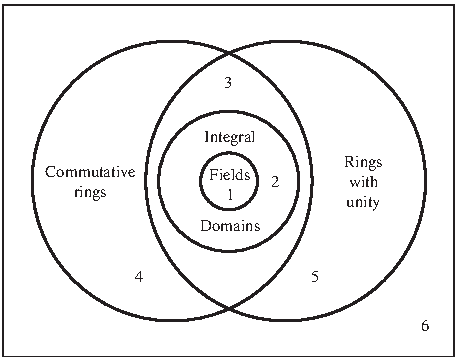
\includegraphics[width=0.626\linewidth,height=.8\textheight,keepaspectratio]{assets/p214_08.pdf}\end{center}
\begin{center}\small\textbf{23.10 Figure}\end{center}
\end{BookFloat}

A collection of rings.

\BookLabel{23.11 Theorem} Every finite integral domain is a field.

\BookLabel{\textit{Proof}} Let \BookInline{R} be a finite integral domain and \BookInline{a} a nonzero element of \BookInline{R.} We wish to show there is an element \BookInline{b\in R} such that \BookInline{ab= 1.} To this end, we define a function \BookInline{f:R\to R} by

\begin{center}\begin{adjustbox}{max width=\linewidth}\BookInline{\displaystyle f(x)= ax.}\end{adjustbox}\end{center}

\noindent We first show that \BookInline{f} is a one-to-one function. Suppose that \BookInline{f(x_{1})= f(x_{2}),\allowbreak } then

\begin{center}\begin{adjustbox}{max width=\linewidth}\BookInline{\displaystyle ax_{1}= ax_{2}}\end{adjustbox}\end{center}

\begin{center}\begin{adjustbox}{max width=\linewidth}\BookInline{\displaystyle x_{1}= x_{2}}\end{adjustbox}\end{center}

\noindent since \BookInline{a\neq 0} and cancellation holds in an integral domain. Thus \BookInline{f} is one-to-one. Since \BookInline{R} is finite and \BookInline{f:R\to R} is one-to-one\BookInline{,\allowbreak f} must also map onto \BookInline{R.} Therefore, there is a \BookInline{b\in R} such that

\begin{center}\begin{adjustbox}{max width=\linewidth}\BookInline{\displaystyle 1= f(a)= ab= ba}\end{adjustbox}\end{center}

\noindent which verifies that \BookInline{a} is a unit. \BookEnd{\blacklozenge}

\end{BookBody}

% Source PDF page 215; original printed page 198
\BookSource{215}{198}
\BookNarrativetrue

\begin{BookBody}

The finite condition in Theorem 23.11 is necessary since \BookInline{\mathbb{Z}} is an infinite integral domain, which is not a field. The counting argument fails in the case where the integral domain is infinite since there are one-to-one functions from an infinite set to itself that are not onto. For example, multiplication by 2 is a one-to-one function mapping \BookInline{\mathbb{Z}} to \BookInline{\mathbb{Z},\allowbreak } but 1 is not in the range of the function.

In Section 39 we will see that other than \BookInline{\mathbb{Z}_{p}} there are many finite integral domains and therefore fields.

\BookTextHeading{\textbf{The Characteristic of a Ring}  }

\noindent Let \BookInline{R} be any ring. We might ask whether there is a positive integer \BookInline{n} such that \BookInline{n\cdot a= 0} for all \BookInline{a\in R,\allowbreak } where \BookInline{n\cdot a} means \BookInline{a+ a+ \cdots + a} for \BookInline{n} summands, as explained in Section 22. For example, the integer \BookInline{m} has this property for the ring \BookInline{\mathbb{Z}_{m}.}

\BookLabel{23.12 Definition} If for a ring \BookInline{R} a positive integer \BookInline{n} exists such that \BookInline{n\cdot a= 0} for all \BookInline{a\in R,\allowbreak } then the least such positive integer is the\textbf{ characteristic of the ring} \BookInline{R.} If no such positive integer exists, then \BookInline{R} is of\textbf{ characteristic} \BookInline{0.}\BookEnd{\blacksquare}

We shall use the concept of a characteristic chiefly for fields. Exercise 35 asks us to show that the characteristic of an integral domain is either 0 or a prime \BookInline{p.}

\BookLabel{23.13 Example} The ring \BookInline{\mathbb{Z}_{n}} is of characteristic \BookInline{n,\allowbreak } while \BookInline{\mathbb{Z},\allowbreak \mathbb{Q},\allowbreak \mathbb{R},\allowbreak } and \BookInline{\mathbb{C}} all have characteristic \BookInline{0.}\BookEnd{\blacktriangle}

At first glance, determination of the characteristic of a ring seems to be a tough job, unless the ring is obviously of characteristic 0. Do we have to examine\textit{ every} element \BookInline{a} of the ring in accordance with Definition 23.12? Our final theorem of this section shows that if the ring has unity, it suffices to examine only \BookInline{a= 1.}

\BookLabel{23.14 Theorem} Let \BookInline{R} be a ring with unity. If \BookInline{n\cdot 1\neq 0} for all \BookInline{n\in \mathbb{Z}^{+ },\allowbreak } then \BookInline{R} has characteristic 0. If \BookInline{n\cdot 1= 0} for some \BookInline{n\in \mathbb{Z}^{+ },\allowbreak } then the smallest such integer \BookInline{n} is the characteristic of \BookInline{R.}

\BookLabel{\textit{Proof}} If \BookInline{n\cdot 1\neq 0} for all \BookInline{n\in \mathbb{Z}^{+ },\allowbreak } then surely we cannot have \BookInline{n\cdot a= 0} for all \BookInline{a\in R} for some positive integer \BookInline{n,\allowbreak } so by Definition \BookInline{23.12,\allowbreak R} has characteristic 0.

Suppose that \BookInline{n} is a positive integer such that \BookInline{n\cdot 1= 0.} Then for any \BookInline{a\in R,\allowbreak } we have

\begin{center}\begin{adjustbox}{max width=\linewidth}\BookInline{\displaystyle n\cdot a= a+ a+ \cdots + a= a(1+ 1+ \cdots + 1)= a(n\cdot 1)= a0= 0.}\end{adjustbox}\end{center}

\noindent Our theorem follows directly. \BookEnd{\blacklozenge}

\end{BookBody}

\BookNarrativefalse

\begin{BookBody}

\BookExerciseTitle{23} \BookEnd{\blacksquare}

\BookTextHeading{\textbf{Computations}}

\BookExercise{1.}{Find all solutions of the equation \BookInline{x^{3}- 2x^{2}- 3x= 0} in \BookInline{\mathbb{Z}_{12}.}}

\BookExercise{2.}{Solve the equation \BookInline{3x= 2} in the field \BookInline{\mathbb{Z}_{7};} in the field \BookInline{\mathbb{Z}_{23}.}}

\BookExercise{3.}{Find all solutions of the equation \BookInline{x^{2}+ 2x+ 2= 0} in \BookInline{\mathbb{Z}_{6}.}}

\BookExercise{4.}{Find all solutions of \BookInline{x^{2}+ 2x+ 4= 0} in \BookInline{\mathbb{Z}_{6}.}}

\noindent In Exercises 5 through 10, find the characteristic of the given ring.

\BookExercise{5.}{\BookInline{2\mathbb{Z}}}

\BookExercise{6.}{\BookInline{\mathbb{Z}\times \mathbb{Z}}}

\BookExercise{7.}{\BookInline{\mathbb{Z}_{3}\times 3\mathbb{Z}}}

\BookExercise{8.}{\BookInline{\mathbb{Z}_{3}\times \mathbb{Z}_{3}}}

\BookExercise{9.}{\BookInline{\mathbb{Z}_{3}\times \mathbb{Z}_{4}}}

\BookExercise{10.}{\BookInline{\mathbb{Z}_{6}\times \mathbb{Z}_{15}}}

\end{BookBody}

% Source PDF page 216; original printed page 199
\BookSource{216}{199}
\BookNarrativefalse

\begin{BookBody}

\noindent In Exercises 11 through 16, classify each nonzero element of the ring as a unit, a divisor of 0, or neither.

\BookExercise{11.}{\BookInline{\mathbb{Z}_{6}}}

\BookExercise{12.}{\BookInline{\mathbb{Z}_{8}}}

\BookExercise{13.}{\BookInline{\mathbb{Z}_{15}}}

\BookExercise{14.}{\BookInline{\mathbb{Z}}}

\BookExercise{15.}{\BookInline{\mathbb{Z}_{3}\times \mathbb{Z}_{3}}}

\BookExercise{16.}{\BookInline{\mathbb{Z}_{4}\times \mathbb{Z}_{5}}}

\BookExercise{17.}{Let \BookInline{R} be a commutative ring with unity of characteristic 4. Compute and simplify \BookInline{(a+ b)^{4}} for \BookInline{a,\allowbreak b\in R.}}

\BookExercise{18.}{Let \BookInline{R} be a commutative ring with unity of characteristic 3. Compute and simplify \BookInline{(a+ b)^{9}} for \BookInline{a,\allowbreak b\in R.}}

\BookExercise{19.}{Let \BookInline{R} be a commutative ring with unity of characteristic 3. Compute and simplify \BookInline{(a+ b)^{6}} for \BookInline{a,\allowbreak b\in R.}}

\BookInline{\Big[\Big]}

\BookExercise{20.}{Show that the matrix \BookInline{\begin{bmatrix} 1 & 2 \\ 2 & 4 \end{bmatrix}} is a divisor of zero in \BookInline{M_{2}(\mathbb{Z}).}}

\BookTextHeading{\textbf{Concepts}}

\noindent In Exercises 21 and 22, correct the definition of the italicized term without reference to the text, if correction is needed, so that it is in a form acceptable for publication.

\BookExercise{21.}{If \BookInline{ab= 0,\allowbreak } then \BookInline{a} and \BookInline{b} are\textit{ divisors of zero}.}

\BookExercise{22.}{If \BookInline{n\cdot a= 0} for all elements \BookInline{a} in a ring \BookInline{R,\allowbreak } then \BookInline{n} is the\textit{ characteristic of} \BookInline{R.}}

\BookExercise{23.}{Determine whether each of the following is true or false.}

\BookExercise{a.}{\textbf{a}\BookInline{.n\mathbb{Z}} has zero divisors if \BookInline{n} is not prime.}

\BookExercise{b.}{Every field is an integral domain.}

\BookExercise{c.}{The characteristic of \BookInline{n\mathbb{Z}} is \BookInline{n.}}

\BookExercise{d.}{As a ring\BookInline{,\allowbreak \mathbb{Z}} is isomorphic to \BookInline{n\mathbb{Z}} for all \BookInline{n\geq 1.}}

\BookExercise{e.}{The cancellation law holds in any ring that is isomorphic to an integral domain.}

\BookExercise{f.}{Every integral domain of characteristic 0 is infinite.}

\BookExercise{g.}{The direct product of two integral domains is again an integral domain.}

\BookExercise{h.}{A divisor of zero in a commutative ring with unity can have no multiplicative inverse.}

\BookExercise{i.}{\textbf{i}\BookInline{.n\mathbb{Z}} is a subdomain of \BookInline{\mathbb{Z}.}}

\BookExercise{j.}{\textbf{j}\BookInline{.\mathbb{Z}} is a subfield of \BookInline{\mathbb{Q}.}}

\BookExercise{24.}{Each of the six numbered regions in Fig. 23.10 corresponds to a certain type of a ring. Give an example of a ring in each of the six cells. For example, a ring in the region numbered 3 must be commutative (it is inside the commutative circle), have unity, but not be an integral domain.}

\BookExercise{25.}{(For students who have had a semester of linear algebra) Let \BookInline{F} be a field. Give five different characterizations of the elements \BookInline{A} of \BookInline{M_{n}(F)} that are divisors of 0.}

\BookExercise{26.}{Redraw Fig. 23.10 to include a subset corresponding to strictly skew fields.}

\BookLabel{\textit{Proof}} \textbf{ Synopsis}

\BookExercise{27.}{Give a one-sentence synopsis of the proof of the “if” part of Theorem 23.6.}

\BookExercise{28.}{Give a two-sentence synopsis of the proof of Theorem 23.11.}

\BookTextHeading{\textbf{Theory}}

\BookExercise{29.}{An element \BookInline{a} of a ring \BookInline{R} is\textbf{ idempotent} if \BookInline{a^{2}= a.} Show that a division ring contains exactly two idempotent elements.}

\BookExercise{30.}{Show that an intersection of subdomains of an integral domain \BookInline{D} is again a subdomain of \BookInline{D.}}

\BookExercise{31.}{Show that a finite ring \BookInline{R} with unity \BookInline{1\neq 0} and no divisors of 0 is a division ring. (It is actually a field, although commutativity is not easy to prove. See Theorem 32.10.) [\textit{Note:} In your proof, to show that \BookInline{a\neq 0} is a unit, you must show that a “left multiplicative inverse” of \BookInline{a\neq 0} in \BookInline{R} is also a “right multiplicative inverse.”]}

\end{BookBody}

% Continuation on source PDF page 217, preceding Section 24
\BookNarrativefalse

\begin{BookBody}

\BookExercise{32.}{Let \BookInline{R} be a ring that contains at least two elements. Suppose for each nonzero \BookInline{a\in R,\allowbreak } there exists a unique \BookInline{b\in R} such that \BookInline{aba= a.}}

\BookExercise{a.}{Show that \BookInline{R} has no divisors of 0.}

\BookExercise{b.}{Show that \BookInline{bab= b.}}

\BookExercise{c.}{Show that \BookInline{R} has unity.}

\BookExercise{d.}{Show that \BookInline{R} is a division ring.}

\BookExercise{33.}{Show that the characteristic of a subdomain of an integral domain \BookInline{D} is equal to the characteristic of \BookInline{D.}}

\BookExercise{34.}{Show that if \BookInline{D} is an integral domain, then \BookInline{\{n\cdot 1\mid n\in \mathbb{Z}\}} is a subdomain of \BookInline{D} contained in every subdomain of \BookInline{D.}}

\BookExercise{35.}{Show that the characteristic of an integral domain \BookInline{D} must be either 0 or a prime \BookInline{p.[}\textit{Hint:} If the characteristic of \BookInline{D} is \BookInline{mn,\allowbreak } consider \BookInline{(m\cdot 1)(n\cdot 1)} in \BookInline{D.]}}

\BookExercise{36.}{This exercise shows that every ring \BookInline{R} can be enlarged (if necessary) to a ring \BookInline{S} with unity, having the same characteristic as \BookInline{R.} Let \BookInline{S= R\times \mathbb{Z}} if \BookInline{R} has characteristic 0, and \BookInline{R\times \mathbb{Z}_{n}} if \BookInline{R} has characteristic \BookInline{n.} Let addition in \BookInline{S} be the usual addition by components, and let multiplication be defined by}

\begin{center}\begin{adjustbox}{max width=\linewidth}\BookInline{\displaystyle (r_{1},\allowbreak n_{1})(r_{2},\allowbreak n_{2})= (r_{1}r_{2}+ n_{1}\cdot r_{2}+ n_{2}\cdot r_{1},\allowbreak n_{1}n_{2})}\end{adjustbox}\end{center}

where \BookInline{n\cdot r} has the meaning explained in Section 22.

\BookExercise{a.}{Show that \BookInline{S} is a ring.}

\BookExercise{b.}{Show that \BookInline{S} has unity.}

\BookExercise{c.}{Show that \BookInline{S} and \BookInline{R} have the same characteristic.}

\BookExercise{d.}{Show that the map \BookInline{\phi:R\to S} given by \BookInline{\phi (r)= (r,\allowbreak 0)} for \BookInline{r\in R} maps \BookInline{R} isomorphically onto a subring of \BookInline{S.}}

\end{BookBody}
\ifdefined\BookMaster\let\BookFinish\relax\else\def\BookFinish{\end{document}}\fi\BookFinish

\clearpage
% !TeX program = xelatex
\ifdefined\BookMaster\else
\documentclass[11pt,oneside]{article}
% !TeX program = xelatex
\usepackage[b5paper,left=22mm,right=22mm,top=20mm,bottom=22mm,footskip=11mm]{geometry}
\usepackage{fontspec}
\setmainfont{TeX Gyre Termes}
\setsansfont{TeX Gyre Heros}
\usepackage{amsmath,amssymb,mathtools,amsthm}
\renewcommand{\cdots}{\mathinner{\cdotp\cdotp\cdotp}}
\usepackage{graphicx,adjustbox,array,booktabs,longtable,multirow,enumitem,changepage,needspace}
\usepackage[table]{xcolor}
\usepackage{fancyhdr}
\raggedbottom
\interfootnotelinepenalty=10000
\newcommand{\BookFootnote}[2]{\begingroup\renewcommand{\thefootnote}{\fnsymbol{footnote}}\footnote[#1]{#2}\endgroup}
\newcommand{\BookFootnoteMark}[1]{\begingroup\renewcommand{\thefootnote}{\fnsymbol{footnote}}\footnotemark[#1]\endgroup}
\newcommand{\BookFootnoteText}[2]{\begingroup\renewcommand{\thefootnote}{\fnsymbol{footnote}}\footnotetext[#1]{#2}\endgroup}
\newenvironment{BookFloat}[1]{\par\addvspace{.6\baselineskip}\noindent\def\BookFloatID{#1}\begin{minipage}{\linewidth}\phantomsection\label{bookfloat:#1:start}}{\phantomsection\label{bookfloat:\BookFloatID:end}\end{minipage}\par\addvspace{.6\baselineskip}}

\usepackage[unicode,hidelinks]{hyperref}
\pagestyle{fancy}
\fancyhf{}
\newcommand{\BookFooter}{}
\fancyfoot[L]{\parbox[b]{\dimexpr\textwidth-15mm}{\footnotesize\BookFooter}}
\fancyfoot[R]{\footnotesize\thepage}
\renewcommand{\headrulewidth}{0pt}
\renewcommand{\footrulewidth}{0pt}
\setlength{\parindent}{0pt}
\setlength{\parskip}{0.2em}
\setlength{\emergencystretch}{3em}
\setlist{nosep,leftmargin=1.7em,labelsep=.65em}
\newif\ifBookNarrative
\BookNarrativetrue
\newenvironment{BookBody}{\setlength{\parindent}{0pt}}{}
\newcommand{\BookStatement}[1]{\par\addvspace{.6\baselineskip}\noindent #1\enspace\ignorespaces}
\newcommand{\BookLabel}[1]{\par\addvspace{.6\baselineskip}\needspace{3\baselineskip}\noindent\textbf{#1}\quad\ignorespaces}
\newcommand{\BookHeading}[1]{\par\addvspace{\baselineskip}\needspace{4\baselineskip}\noindent{\large\bfseries #1}\par\medskip}
\newcommand{\BookSubheading}[1]{\par\addvspace{.7\baselineskip}\needspace{3\baselineskip}\noindent{\bfseries #1}\par\smallskip}
\newcommand{\BookTextHeading}[1]{\par\addvspace{.7\baselineskip}\needspace{3\baselineskip}\noindent #1\par\smallskip}
\newcommand{\BookSectionTitle}[2]{\par\addvspace{1.2\baselineskip}\needspace{5\baselineskip}\noindent\colorbox{gray!25}{\sffamily\bfseries\small SECTION #1}\quad{\large\bfseries #2}\par\medskip}
\newcommand{\BookExerciseTitle}[1]{\par\addvspace{\baselineskip}\needspace{4\baselineskip}\noindent{\color{gray}\rule{1.5mm}{1.5mm}}\enspace{\large\bfseries Exercises #1}\par\medskip}
\newcommand{\BookBullet}[1]{\begin{list}{\textbullet}{\setlength{\leftmargin}{1.7em}\setlength{\labelwidth}{1em}\setlength{\labelsep}{.7em}\setlength{\topsep}{0pt}\setlength{\parsep}{0pt}\setlength{\itemsep}{0pt}}\item #1\end{list}}
\newcommand{\BookExercise}[2]{\begin{list}{\textbf{#1}}{\setlength{\leftmargin}{2.2em}\setlength{\labelwidth}{1.5em}\setlength{\labelsep}{.7em}\setlength{\topsep}{.15em}\setlength{\parsep}{0pt}\setlength{\itemsep}{0pt}}\item #2\end{list}}
\newcommand{\BookEnd}[1]{\unskip\nobreak\hfill\ensuremath{#1}}
\newcommand{\BookSource}[2]{\phantomsection\label{sourcepage:#1}} % Source-page anchors, retained through reflow.
\usepackage{multicol}
\usepackage{tikz}
\newcommand{\BookPartEntry}[2]{\par\noindent\makebox[17mm][l]{\bfseries Section #1}#2\par}
\newcommand{\BookPartTitle}[3]{\par\bigskip\noindent\begin{tikzpicture}\node[anchor=north west,inner sep=0pt,outer sep=0pt] (bookpart) at (0,0) {\begin{minipage}{\dimexpr\linewidth-.5pt}\hspace*{26mm}\begin{minipage}[t]{\dimexpr\linewidth-26mm}\begin{adjustbox}{max width=\linewidth}{\fontsize{20}{24}\selectfont\bfseries #2}\end{adjustbox}\par\vspace{6mm}\hrule\vspace{6mm}{\sffamily\footnotesize\setlength{\parskip}{.3em}#3}\vspace{3mm}\end{minipage}\end{minipage}};\path[shade,top color=gray!60,bottom color=white] (0,0) rectangle ([xshift=24mm]bookpart.south west);\node[anchor=north,font=\sffamily\bfseries\small] at (12mm,-2mm) {PART};\node[anchor=north,font=\sffamily\bfseries\Huge] at (12mm,-7mm) {#1};\end{tikzpicture}\par\bigskip}
\newsavebox{\BookMathBox}
\makeatletter
\newcommand{\BookInline}[1]{\leavevmode\hskip0pt\relax\begingroup\in@{\begin}{#1}\ifin@\sbox{\BookMathBox}{\(#1\)}\ifdim\wd\BookMathBox>\dimexpr\linewidth-1em\relax\resizebox{\dimexpr\linewidth-1em\relax}{!}{\usebox{\BookMathBox}}\else\(#1\)\fi\else\in@{\left}{#1}\ifin@\sbox{\BookMathBox}{\(#1\)}\ifdim\wd\BookMathBox>\dimexpr\linewidth-1em\relax\resizebox{\dimexpr\linewidth-1em\relax}{!}{\usebox{\BookMathBox}}\else\(#1\)\fi\else\(#1\)\fi\fi\endgroup\hskip0pt\relax}
\makeatother
\DeclareMathOperator{\Aut}{Aut}
\DeclareMathOperator{\End}{End}
\DeclareMathOperator{\Hom}{Hom}
\DeclareMathOperator{\GF}{GF}
\DeclareMathOperator{\irr}{irr}
\DeclareMathOperator{\lt}{lt}
\DeclareMathOperator{\lp}{lp}
\providecommand{\textcircled}[1]{\textnormal{(#1)}}

\begin{document}
\fi
\renewcommand{\BookFooter}{Section 24 Fermat’s and Euler’s Theorems}
\pdfbookmark[0]{Section 24 Fermat’s and Euler’s Theorems}{24_fermat_s_and_euler_s_theorems}
\ifdefined\BookMaster\else\setcounter{page}{200}\fi
% Source PDF page 217; original printed page 200
\BookSource{217}{200}
\BookNarrativetrue

\begin{BookBody}

\BookSectionTitle{24}{Fermat’s and Euler’s Theorems}

\BookTextHeading{\textbf{Fermat’s Theorem}  }

\noindent We know that as additive groups\BookInline{,\allowbreak \mathbb{Z}_{n}} and \BookInline{\mathbb{Z}/n\mathbb{Z}} are naturally isomorphic, with the coset \BookInline{a+ n\mathbb{Z}} corresponding to \BookInline{a} for each \BookInline{a\in \mathbb{Z}_{n}.} Furthermore, addition of cosets in \BookInline{\mathbb{Z}/n\mathbb{Z}} may be performed by choosing any representatives, adding them in \BookInline{\mathbb{Z},\allowbreak } and finding the coset of \BookInline{n\mathbb{Z}} containing their sum. It is easy to see that \BookInline{\mathbb{Z}/n\mathbb{Z}} can be made into a ring by multiplying cosets in the same fashion, that is, by multiplying any chosen representatives. While we will be showing this later in a more general situation, we do this special case now. We need only show that such coset multiplication is well defined, because the associativity of multiplication and the distributive laws will follow immediately from those properties of the chosen representatives in \BookInline{\mathbb{Z}.} To this end, choose representatives \BookInline{a+ rn} and \BookInline{b+ sn,\allowbreak } rather than \BookInline{a} and \BookInline{b,\allowbreak } from the cosets \BookInline{a+ n\mathbb{Z}} and \BookInline{b+ n\mathbb{Z}.} Then

\begin{center}\begin{adjustbox}{max width=\linewidth}\BookInline{\displaystyle (a+ rn)(b+ sn)= ab+ (as+ rb+ rsn)n,\allowbreak }\end{adjustbox}\end{center}

\noindent which is also an element of \BookInline{ab+ n\mathbb{Z}.} Thus the multiplication is well-defined, and our cosets form a ring isomorphic to the ring \BookInline{\mathbb{Z}_{n}.}

Exercise 39 in Section 22 asks us to show that the units in a ring form a group under the multiplication operation of the ring. This is a very useful fact that we will use to provide simple proofs for both Fermat’s Little Theorem and Euler’s generalization. We start with Fermat’s Theorem.

\BookLabel{24.1 Theorem} \textbf{(Little Theorem of Fermat)} If \BookInline{a\in \mathbb{Z}} and \BookInline{p} is a prime not dividing \BookInline{a,\allowbreak } then \BookInline{p} divides \BookInline{a^{p- 1}- 1,\allowbreak } that is\BookInline{,\allowbreak a^{p- 1}\equiv 1(}mod \BookInline{p)} for \BookInline{a\not \equiv 0(}mod \BookInline{p).}

\BookLabel{\textit{Proof}} The ring \BookInline{\mathbb{Z}_{p}} is a field, which implies that all the nonzero elements are units. Thus \BookInline{\langle \mathbb{Z}_{p}^{\ast },\allowbreak \cdot \rangle } is a group with \BookInline{p- 1} elements. Any \BookInline{b} in the group \BookInline{\mathbb{Z}_{p}^{\ast }} has order a divisor of \BookInline{|\mathbb{Z}_{p}^{\ast }|= } \BookInline{p- 1.} Therefore

\end{BookBody}

% Source PDF page 218; original printed page 201
\BookSource{218}{201}
\BookNarrativetrue

\begin{BookBody}

\begin{center}\begin{adjustbox}{max width=\linewidth}\BookInline{\displaystyle b^{p- 1}= 1\in \mathbb{Z}_{p}.}\end{adjustbox}\end{center}

The rings \BookInline{\mathbb{Z}_{p}} and \BookInline{\mathbb{Z}/p\mathbb{Z}} are isomorphic where the element \BookInline{b\in \mathbb{Z}_{p}} corresponds to the coset \BookInline{b+ p\mathbb{Z}.} For any integer \BookInline{a} that is not a multiple of \BookInline{p,\allowbreak a+ p\mathbb{Z}= b+ p\mathbb{Z}} for some \BookInline{0\leq b\leq p- 1.} Thus

\begin{center}\begin{adjustbox}{max width=\linewidth}\BookInline{\displaystyle (a+ p\mathbb{Z})^{p- 1}= (b+ p\mathbb{Z})^{p- 1}= 1+ p\mathbb{Z}\in \mathbb{Z}/p\mathbb{Z}.}\end{adjustbox}\end{center}

\noindent In other words,

\begin{center}\begin{adjustbox}{max width=\linewidth}\BookInline{\displaystyle a^{p- 1}\equiv 1(\;\text{mod}\;p).}\end{adjustbox}\end{center} \BookEnd{\blacklozenge}

\BookLabel{24.2 Corollary} If \BookInline{a\in \mathbb{Z},\allowbreak } then \BookInline{a^{p}\equiv a(}mod \BookInline{p)} for any prime \BookInline{p.}

\BookLabel{\textit{Proof}} The corollary follows from Theorem 24.1 if \BookInline{a\not \equiv 0(}mod \BookInline{p).} If \BookInline{a\equiv 0(}mod \BookInline{p),\allowbreak } then both sides reduce to 0 modulo \BookInline{p.}\BookEnd{\blacklozenge}

\BookLabel{24.3 Example} Let us compute the remainder of 8103 when divided by 13. Using Fermat’s theorem, we have

\begin{center}\begin{adjustbox}{max width=\linewidth}\BookInline{\displaystyle \begin{aligned}&8^{103}\equiv (8^{12})^{8}(8^{7})\equiv (1^{8})(8^{7})\equiv 8^{7}\equiv (- 5)^{7} \\ &\equiv (25)^{3}(- 5)\equiv (- 1)^{3}(- 5)\equiv 5(\;\text{mod}\;13).\end{aligned}}\end{adjustbox}\end{center} \BookEnd{\blacktriangle}

\BookTextHeading{\ensuremath{\blacksquare} \textbf{HISTORICAL NOTE}  }

\noindent The statement of Theorem 24.1 occurs in a letter from Pierre de Fermat (1601–1665) to Bernard Frenicle de Bessy, dated 18 October 1640. Fermat’s version of the theorem was that for any prime \BookInline{p} and any geometric progression \BookInline{a,\allowbreak a^{2},\allowbreak \cdots,\allowbreak a^{t},\allowbreak \cdots,\allowbreak } there is a least number \BookInline{a^{T}} of the progression such that \BookInline{p} divides \BookInline{a^{T}- 1.} Furthermore\BookInline{,\allowbreak T} divides \BookInline{p- 1} and \BookInline{p} also divides all numbers of the form \BookInline{a^{KT}- 1.(}It is curious that Fermat failed to note the condition that \BookInline{p} not divide \BookInline{a;} perhaps he felt that it was obvious that the result fails in that case.)

\noindent Fermat did not in the letter or elsewhere indicate a proof of the result and, in fact, never mentioned it again. But we can infer from other parts of this correspondence that Fermat’s interest in this result came from his study of perfect numbers. (A perfect number is a positive integer \BookInline{m} that is the sum of all of its divisors less than \BookInline{m;} for example\BookInline{,\allowbreak 6= 1+ 2+ 3} is a perfect number.) Euclid had shown that \BookInline{2^{n- 1}(2^{n}- 1)} is perfect if \BookInline{2^{n}- 1} is prime. The question then was to find methods for determining whether \BookInline{2^{n}- 1} was prime. Fermat noted that \BookInline{2^{n}- 1} was composite if \BookInline{n} is composite, and then derived from his theorem the result that if \BookInline{n} is prime, the only possible divisors of \BookInline{2^{n}- 1} are those of the form \BookInline{2kn+ 1.} From this result he was able quickly to show, for example, that \BookInline{2^{37}- 1} was divisible by \BookInline{223= 2\cdot 3\cdot 37+ 1.}

\BookLabel{24.4 Example} Show that \BookInline{2^{11,\allowbreak 213}- 1} is not divisible by 11.

\BookLabel{\textit{Solution}} By Fermat’s theorem\BookInline{,\allowbreak 2^{10}\equiv 1(}mod 11), so

\begin{center}\begin{adjustbox}{max width=\linewidth}\BookInline{\displaystyle \begin{aligned}&2^{11,\allowbreak 213}- 1\equiv [(2^{10})^{1,\allowbreak 121}\cdot 2^{3}]- 1\equiv [1^{1,\allowbreak 121}\cdot 2^{3}]- 1 \\ &\equiv 2^{3}- 1\equiv 8- 1\equiv 7(\;\text{mod}\;11).\end{aligned}}\end{adjustbox}\end{center}

\noindent Thus the remainder of \BookInline{2^{11,\allowbreak 213}- 1} when divided by 11 is 7, not 0. (The number 11,213 is prime, and it has been shown that \BookInline{2^{11,\allowbreak 213}- 1} is a prime number. Primes of the form \BookInline{2^{p}- 1} where \BookInline{p} is prime are known as\textbf{ Mersenne primes}\BookInline{.)}\BookEnd{\blacktriangle}

\end{BookBody}

% Source PDF page 219; original printed page 202
\BookSource{219}{202}
\BookNarrativetrue

\begin{BookBody}

\BookLabel{24.5 Example} Show that for every integer \BookInline{n,\allowbreak } the number \BookInline{n^{33}- n} is divisible by 15.

\BookLabel{\textit{Solution}} This seems like an incredible result. It means that 15 divides \BookInline{2^{33}- 2,\allowbreak 3^{33}- 3,\allowbreak 4^{33}- 4,\allowbreak } etc.

Now \BookInline{15= 3\cdot 5,\allowbreak } and we shall use Fermat’s theorem to show that \BookInline{n^{33}- n} is divisible by both 3 and 5 for every \BookInline{n.} Note that \BookInline{n^{33}- n= n(n^{32}- 1).}

If 3 divides \BookInline{n,\allowbreak } then surely 3 divides \BookInline{n(n^{32}- 1).} If 3 does not divide \BookInline{n,\allowbreak } then by Fermat’s theorem\BookInline{,\allowbreak n^{2}\equiv 1(}mod 3) so

\begin{center}\begin{adjustbox}{max width=\linewidth}\BookInline{\displaystyle n^{32}- 1\equiv (n^{2})^{16}- 1\equiv 1^{16}- 1\equiv 0(\;\text{mod}\;3),\allowbreak }\end{adjustbox}\end{center}

\noindent and hence 3 divides \BookInline{n^{32}- 1.}

If \BookInline{n\equiv 0(}mod 5), then \BookInline{n^{33}- n\equiv 0(}mod 5). If \BookInline{n\not \equiv 0(}mod 5), then by Fermat’s theorem\BookInline{,\allowbreak n^{4}\equiv 1(}mod 5), so

\begin{center}\begin{adjustbox}{max width=\linewidth}\BookInline{\displaystyle n^{32}- 1\equiv (n^{4})^{8}- 1\equiv 1^{8}- 1\equiv 0(\;\text{mod}\;5).}\end{adjustbox}\end{center}

\noindent Thus \BookInline{n^{33}- n\equiv 0(}mod 5) for every \BookInline{n} also. \BookEnd{\blacktriangle}

\BookTextHeading{\textbf{Euler’s Generalization}  }

\noindent Theorem 23.3 classifies all the elements in \BookInline{\mathbb{Z}_{n}} into three categories. An element \BookInline{k} in \BookInline{\mathbb{Z}_{n}} is either 0, a unit if the gcd\BookInline{(n,\allowbreak k)= 1,\allowbreak } or else a divisor of 0 if gcd\BookInline{(n,\allowbreak k)>1.} Exercise 39 in Section 22 shows that the units in a ring form a group under multiplication. Therefore, the set of nonzero elements in \BookInline{\mathbb{Z}_{n},\allowbreak } which are relatively prime to \BookInline{n,\allowbreak } form a multiplicative group. Euler’s generalization of Fermat’s theorem is based on the number of units in \BookInline{\mathbb{Z}_{n}.}

Let \BookInline{n} be a positive integer. Let \BookInline{\varphi (n)} be defined as the number of positive integers less than or equal to \BookInline{n} and relatively prime to \BookInline{n.} Note that \BookInline{\varphi (1)= 1.}

\BookLabel{24.6 Example} Let \BookInline{n= 12.} The positive integers less than or equal to 12 and relatively prime to 12 are 1, 5, 7, and 11, so \BookInline{\varphi (12)= 4.}\BookEnd{\blacktriangle}

By Theorem \BookInline{23.3,\allowbreak \varphi (n)} is the number of nonzero elements of \BookInline{\mathbb{Z}_{n}} that are not divisors of 0. This function \BookInline{\varphi:\mathbb{Z}^{+ }\to \mathbb{Z}^{+ }} is the\textbf{ Euler phi-function.} We can now describe Euler’s generalization of Fermat’s theorem.

\BookLabel{24.7 Theorem} \textbf{(Euler’s Theorem)} If \BookInline{a} is an integer relatively prime to \BookInline{n,\allowbreak } then \BookInline{a^{\varphi (n)}- 1} is divisible by \BookInline{n,\allowbreak } that is\BookInline{,\allowbreak a^{\varphi (n)}\equiv 1(}mod \BookInline{n).}

\BookLabel{\textit{Proof}} If \BookInline{a} is relatively prime to \BookInline{n,\allowbreak } then the coset \BookInline{a+ n\mathbb{Z}} of \BookInline{n\mathbb{Z}} containing \BookInline{a} contains an integer \BookInline{b<n} and relatively prime to \BookInline{n.} Using the fact that multiplication of these cosets by multiplication modulo \BookInline{n} of representatives is well-defined, we have

\begin{center}\begin{adjustbox}{max width=\linewidth}\BookInline{\displaystyle a^{\varphi (n)}\equiv b^{\varphi (n)}(\;\text{mod}\;n).}\end{adjustbox}\end{center}

\noindent But by Theorem \BookInline{23.3,\allowbreak b} can be viewed as an element of the multiplicative group \BookInline{G_{n}} of order \BookInline{\varphi (n)} consisting of the \BookInline{\varphi (n)} elements of \BookInline{\mathbb{Z}_{n}} relatively prime to \BookInline{n.} Thus

\begin{center}\begin{adjustbox}{max width=\linewidth}\BookInline{\displaystyle b^{\varphi (n)}\equiv 1(\;\text{mod}\;n),\allowbreak }\end{adjustbox}\end{center}

\noindent and our theorem follows. \BookEnd{\blacklozenge}

\BookLabel{24.8 Example} Let \BookInline{n= 12.} We saw in Example 24.6 that \BookInline{\varphi (12)= 4.} Thus if we take any integer \BookInline{a} relatively prime to 12, then \BookInline{a^{4}\equiv 1(}mod 12). For example, with \BookInline{a= 7,\allowbreak } we have \BookInline{7^{4}= } \BookInline{(49)^{2}= 2,\allowbreak 401= 12(200)+ 1,\allowbreak } so \BookInline{7^{4}\equiv 1(}mod 12). Of course, the easy way to compute 74 (mod 12), without using Euler’s theorem, is to compute it in \BookInline{\mathbb{Z}_{12}.} In \BookInline{\mathbb{Z}_{12},\allowbreak } we have \BookInline{7= - 5} so

\begin{center}\begin{adjustbox}{max width=\linewidth}\BookInline{\displaystyle 7^{2}= (- 5)^{2}= (5)^{2}= 1\;\text{and}\;7^{4}= 1^{2}= 1.}\end{adjustbox}\end{center} \BookEnd{\blacktriangle}

\end{BookBody}

% Source PDF page 220; original printed page 203
\BookSource{220}{203}
\BookNarrativetrue

\begin{BookBody}

\BookTextHeading{\textbf{Application to} \textit{\textbf{ax}} \ensuremath{\equiv} \textit{\textbf{b}} \textbf{(mod} \textit{\textbf{m}}\textbf{)}      }

\noindent We can find all solutions of a linear congruence\textit{ ax} \BookInline{\equiv b(}mod \BookInline{m).} We prefer to work with an equation in \BookInline{\mathbb{Z}_{m}} and interpret the results for congruences.

\BookLabel{24.9 Theorem} Let \BookInline{m} be a positive integer and let \BookInline{a\in \mathbb{Z}_{m}} be relatively prime to \BookInline{m.} For each \BookInline{b\in \mathbb{Z}_{m},\allowbreak } the equation\textit{ ax} \BookInline{= b} has a unique solution in \BookInline{\mathbb{Z}_{m}.}

\BookLabel{\textit{Proof}} By Theorem \BookInline{23.3,\allowbreak a} is a unit in \BookInline{\mathbb{Z}_{m}} and \BookInline{s= a^{- 1}b} is certainly a solution of the equation. Multiplying both sides of\textit{ ax} \BookInline{= b} on the left by \BookInline{a^{- 1},\allowbreak } we see this is the only solution. \BookEnd{\blacklozenge}

Interpreting this theorem for congruences, we obtain at once the following corollary.

\BookLabel{24.10 Corollary} If \BookInline{a} and \BookInline{m} are relatively prime integers, then for any integer \BookInline{b,\allowbreak } the congruence\textit{ ax} \BookInline{\equiv } \BookInline{b(}mod \BookInline{m)} has as solutions all integers in precisely one residue class modulo \BookInline{m.}\BookEnd{\blacklozenge}

\noindent Theorem 24.9 serves as a lemma for the general case.

\BookLabel{24.11 Theorem} Let \BookInline{m} be a positive integer and let \BookInline{a,\allowbreak b\in \mathbb{Z}_{m}.} Let \BookInline{d} be the gcd of \BookInline{a} and \BookInline{m.} The equation \textit{ax} \BookInline{= b} has a solution in \BookInline{\mathbb{Z}_{m}} if and only if \BookInline{d} divides \BookInline{b.} When \BookInline{d} divides \BookInline{b,\allowbreak } the equation has exactly \BookInline{d} solutions in \BookInline{\mathbb{Z}_{m}.}

\BookLabel{\textit{Proof}} First we show there is no solution of\textit{ ax} \BookInline{= b} in \BookInline{\mathbb{Z}_{m}} unless \BookInline{d} divides \BookInline{b.} Suppose \BookInline{s\in \mathbb{Z}_{m}} is a solution. Then\textit{ as} \BookInline{- b= qm} in \BookInline{\mathbb{Z},\allowbreak } so \BookInline{b= } \textit{as} \BookInline{- qm.} Since \BookInline{d} divides both \BookInline{a} and \BookInline{m,\allowbreak } we see that \BookInline{d} divides the right-hand side of the equation \BookInline{b= } \textit{as} \BookInline{- qm,\allowbreak } and hence divides \BookInline{b.} Thus a solution \BookInline{s} can exist only if \BookInline{d} divides \BookInline{b.}

Suppose now that \BookInline{d} does divide \BookInline{b.} Let

\begin{center}\begin{adjustbox}{max width=\linewidth}\BookInline{\displaystyle a= a_{1}d,\allowbreak b= b_{1}d,\allowbreak \;\text{and}\;m= m_{1}d.}\end{adjustbox}\end{center}

\noindent Then the equation\textit{ as} \BookInline{- b= qm} in \BookInline{\mathbb{Z}} can be rewritten as \BookInline{d(a_{1}s- b_{1})= dqm_{1}.} We see that\textit{ as} \BookInline{- b} is a multiple of \BookInline{m} if and only if \BookInline{a_{1}s- b_{1}} is a multiple of \BookInline{m_{1}.} Thus the solutions \BookInline{s} of\textit{ ax} \BookInline{= b} in \BookInline{\mathbb{Z}_{m}} are precisely the elements that, read modulo \BookInline{m_{1},\allowbreak } yield solutions of \BookInline{a_{1}x= b_{1}} in \BookInline{\mathbb{Z}_{m_{1}}}. Now let \BookInline{s\in \mathbb{Z}_{m_{1}}} be the unique solution of \BookInline{a_{1}x= b_{1}} in \BookInline{\mathbb{Z}_{m_{1}}} given by Theorem 24.9. The numbers in \BookInline{\mathbb{Z}_{m}} that reduce to \BookInline{s} modulo \BookInline{m_{1}} are precisely those that can be computed in \BookInline{\mathbb{Z}_{m}} as

\begin{center}\begin{adjustbox}{max width=\linewidth}\BookInline{\displaystyle s,\allowbreak s+ m_{1},\allowbreak s+ 2m_{1},\allowbreak s+ 3m_{1},\allowbreak \cdots ,\allowbreak s+ (d- 1)m_{1}.}\end{adjustbox}\end{center}

\noindent Thus there are exactly \BookInline{d} solutions of the equation in \BookInline{\mathbb{Z}_{m}.} \BookEnd{\blacklozenge}

Theorem 24.11 gives us at once this classical result on the solutions of a linear congruence.

\BookLabel{24.12 Corollary} Let \BookInline{d} be the gcd of positive integers \BookInline{a} and \BookInline{m.} The congruence\textit{ ax} \BookInline{\equiv b(}mod \BookInline{m)} has a solution if and only if \BookInline{d} divides \BookInline{b.} When this is the case, the solutions are the integers in exactly \BookInline{d} distinct residue classes modulo \BookInline{m.}\BookEnd{\blacklozenge}

Actually, our proof of Theorem 24.11 shows a bit more about the solutions of \textit{ax} \BookInline{\equiv b(}mod \BookInline{m)} than we stated in this corollary; namely, it shows that if any solution \BookInline{s} is found, then the solutions are precisely all elements of the residue classes \BookInline{(s+ km_{1})+ (m\mathbb{Z})} where \BookInline{m_{1}= m/d} and \BookInline{k} runs through the integers from 0 to \BookInline{d- 1.} It also tells us that we can find such an \BookInline{s} by finding \BookInline{a_{1}= a/d} and \BookInline{b_{1}= b/d,\allowbreak } and solving \BookInline{a_{1}x\equiv b_{1}(}mod \BookInline{m_{1}).} To solve this congruence, we may consider \BookInline{a_{1}} and \BookInline{b_{1}} to be replaced by their remainders modulo \BookInline{m_{1}} and solve the equation \BookInline{a_{1}x= b_{1}} in \BookInline{\mathbb{Z}_{m_{1}}}.

\end{BookBody}

% Source PDF page 221; original printed page 204
\BookSource{221}{204}
\BookNarrativetrue

\begin{BookBody}

\BookLabel{24.13 Example} Find all solutions of the congruence \BookInline{12x\equiv 27(}mod 18).

\BookLabel{\textit{Solution}} The gcd of 12 and 18 is 6, and 6 is not a divisor of 27. Thus by the preceding corollary, there are no solutions\BookInline{.}\BookEnd{\blacktriangle}

\BookLabel{24.14 Example} Find all solutions of the congruence \BookInline{15x\equiv 27(}mod 18).

\BookLabel{\textit{Solution}} The gcd of 15 and 18 is 3, and 3 does divide 27. Proceeding as explained before Example 24.13, we divide everything by 3 and consider the congruence \BookInline{5x\equiv 9(}mod 6), which amounts to solving the equation \BookInline{5x= 3} in \BookInline{\mathbb{Z}_{6}.} Now the units in \BookInline{\mathbb{Z}_{6}} are 1 and 5, and 5 is clearly its own inverse in this group of units. Thus the solution in \BookInline{\mathbb{Z}_{6}} is \BookInline{x= (5^{- 1})(3)= (5)(3)= 3.} Consequently, the solutions of \BookInline{15x\equiv 27(}mod 18) are the integers in the three residue classes

\begin{center}\begin{adjustbox}{max width=\linewidth}\BookInline{\displaystyle 3+ 18\mathbb{Z}= \{\cdots ,\allowbreak - 33,\allowbreak - 15,\allowbreak 3,\allowbreak 21,\allowbreak 39,\allowbreak \cdots \},\allowbreak }\end{adjustbox}\end{center}

\begin{center}\begin{adjustbox}{max width=\linewidth}\BookInline{\displaystyle 9+ 18\mathbb{Z}= \{\cdots ,\allowbreak - 27,\allowbreak - 9,\allowbreak 9,\allowbreak 27,\allowbreak 45,\allowbreak \cdots \}.}\end{adjustbox}\end{center}

\begin{center}\begin{adjustbox}{max width=\linewidth}\BookInline{\displaystyle 15+ 18\mathbb{Z}= \{\cdots ,\allowbreak - 21,\allowbreak - 3,\allowbreak 15,\allowbreak 33,\allowbreak 51,\allowbreak \cdots \},\allowbreak }\end{adjustbox}\end{center}

\noindent illustrating Corollary 24.12. Note the \BookInline{d= 3} solutions 3, 9, and 15 in \BookInline{\mathbb{Z}_{18}.} All the solutions in the three displayed residue classes modulo 18 can be collected in the one residue class \BookInline{3+ 6\mathbb{Z}} modulo 6, for they came from the solution \BookInline{x= 3} of \BookInline{5x= 3} in \BookInline{\mathbb{Z}_{6}.}\BookEnd{\blacktriangle}

\end{BookBody}

\BookNarrativefalse

\begin{BookBody}

\BookExerciseTitle{24}

\BookTextHeading{\textbf{Computations}}

\noindent We will see later that the multiplicative group of nonzero elements of a finite field is cyclic. Illustrate this by finding a generator for this group for the given finite field.

\BookExercise{1.}{\BookInline{\mathbb{Z}_{7}}}

\BookExercise{2.}{\BookInline{\mathbb{Z}_{11}}}

\BookExercise{3.}{\BookInline{\mathbb{Z}_{17}}}

\BookExercise{4.}{Using Fermat’s theorem, find the remainder of 347 when it is divided by 23.}

\BookExercise{5.}{Use Fermat’s theorem to find the remainder of 3749 when it is divided by 7.}

\BookExercise{6.}{Compute the remainder of \BookInline{2^{(2^{17})}+ 1} when divided by 19. [\textit{Hint:} You will need to compute the remainder of 217 modulo 18.]}

\BookExercise{7.}{Make a table of values of \BookInline{\varphi (n)} for \BookInline{n\leq 30.}}

\BookExercise{8.}{Compute \BookInline{\varphi (p^{2})} where \BookInline{p} is a prime.}

\BookExercise{9.}{Compute \BookInline{\varphi (pq)} where both \BookInline{p} and \BookInline{q} are primes.}

\BookExercise{10.}{Use Euler’s generalization of Fermat’s theorem to find the remainder of 71000 when divided by 24.}

\noindent In Exercises 11 through 18, describe all solutions of the given congruence, as we did in Examples 24.13 and 24.14.

\BookExercise{11.}{\BookInline{2x\equiv 6(}mod 4)}

\BookExercise{12.}{\BookInline{22x\equiv 5(}mod 15)}

\BookExercise{13.}{\BookInline{36x\equiv 15(}mod 24)}

\BookExercise{14.}{\BookInline{45x\equiv 15(}mod 24)}

\BookExercise{15.}{\BookInline{39x\equiv 125(}mod 9)}

\BookExercise{16.}{\BookInline{41x\equiv 125(}mod 9)}

\BookExercise{17.}{\BookInline{155x\equiv 75(}mod 65)}

\BookExercise{18.}{\BookInline{39x\equiv 52(}mod 130)}

\BookExercise{19.}{Let \BookInline{p} be a prime \BookInline{\geq 3.} Use Exercise 28 below to find the remainder of \BookInline{(p- 2)}! modulo \BookInline{p.}}

\BookExercise{20.}{Using Exercise 28 below, find the remainder of 34! modulo 37.}

\BookExercise{21.}{Using Exercise 28 below, find the remainder of 49! modulo 53.}

\BookExercise{22.}{Using Exercise 28 below, find the remainder of 24! modulo 29.}

\end{BookBody}

% Continuation on source PDF page 222, preceding Section 25
\BookNarrativefalse

\begin{BookBody}

\BookTextHeading{\textbf{Concepts}}

\BookExercise{23.}{Determine whether each of the following is true or false.}

\BookExercise{a.}{\textbf{a}\BookInline{.a^{p- 1}\equiv 1(}mod \BookInline{p)} for all integers \BookInline{a} and primes \BookInline{p.}}

\BookExercise{b.}{\textbf{b}\BookInline{.a^{p- 1}\equiv 1(}mod \BookInline{p)} for all integers \BookInline{a} such that \BookInline{a\not \equiv 0(}mod \BookInline{p)} for a prime \BookInline{p.}}

\BookExercise{c.}{\textbf{c}\BookInline{.\varphi (n)\leq n} for all \BookInline{n\in \mathbb{Z}^{+ }.}}

\BookExercise{d.}{\textbf{d}\BookInline{.\varphi (n)\leq n- 1} for all \BookInline{n\in \mathbb{Z}^{+ }.}}

\BookExercise{e.}{The units in \BookInline{\mathbb{Z}_{n}} are the positive integers less than \BookInline{n} and relatively prime to \BookInline{n.}}

\BookExercise{f.}{The product of two units in \BookInline{\mathbb{Z}_{n}} is always a unit.}

\BookExercise{g.}{The product of two nonunits in \BookInline{\mathbb{Z}_{n}} may be a unit.}

\BookExercise{h.}{The product of a unit and a nonunit in \BookInline{\mathbb{Z}_{n}} is never a unit.}

\BookExercise{i.}{Every congruence\textit{ ax} \BookInline{\equiv b(}mod \BookInline{p),\allowbreak } where \BookInline{p} is a prime, has a solution.}

\BookExercise{j.}{Let \BookInline{d} be the gcd of positive integers \BookInline{a} and \BookInline{m.} If \BookInline{d} divides \BookInline{b,\allowbreak } then the congruence\textit{ ax} \BookInline{\equiv b(}mod \BookInline{m)} has exactly \BookInline{d} incongruent solutions.}

\BookExercise{24.}{Give the group multiplication table for the multiplicative group of units in \BookInline{\mathbb{Z}_{12}.} To which group of order 4 is it isomorphic?}

\BookLabel{\textit{Proof}} \textbf{ Synopsis}

\BookExercise{25.}{Give a one-sentence synopsis of the proof of Theorem 24.1.}

\BookExercise{26.}{Give a one-sentence synopsis of the proof of Theorem 24.7.}

\BookTextHeading{\textbf{Theory}}

\BookExercise{27.}{Show that 1 and \BookInline{p- 1} are the only elements of the field \BookInline{\mathbb{Z}_{p}} that are their own multiplicative inverse. [\textit{Hint:} Consider the equation \BookInline{x^{2}- 1= 0.]}}

\BookExercise{28.}{Using Exercise 27, deduce the half of\textit{ Wilson’}\BookInline{s} \textit{theorem} that states that if \BookInline{p} is a prime, then \BookInline{(p- 1)!\equiv - 1} (mod \BookInline{p).[}The other half states that if \BookInline{n} is an integer \BookInline{>1} such that \BookInline{(n- 1)!\equiv - 1(}mod \BookInline{n),\allowbreak } then \BookInline{n} is a prime. Just think what the remainder of \BookInline{(n- 1)}! would be modulo \BookInline{n} if \BookInline{n} is not a prime.]}

\BookExercise{29.}{Use Fermat’s theorem to show that for any positive integer \BookInline{n,\allowbreak } the integer \BookInline{n^{37}- n} is divisible by 383838. [\textit{Hint:} \BookInline{383838= (37)(19)(13)(7)(3)(2).]}}

\BookExercise{30.}{Referring to Exercise 29, find a number larger than 383838 that divides \BookInline{n^{37}- n} for all positive integers \BookInline{n.}}

\end{BookBody}
\ifdefined\BookMaster\let\BookFinish\relax\else\def\BookFinish{\end{document}}\fi\BookFinish

\clearpage
% !TeX program = xelatex
\ifdefined\BookMaster\else
\documentclass[11pt,oneside]{article}
% !TeX program = xelatex
\usepackage[b5paper,left=22mm,right=22mm,top=20mm,bottom=22mm,footskip=11mm]{geometry}
\usepackage{fontspec}
\setmainfont{TeX Gyre Termes}
\setsansfont{TeX Gyre Heros}
\usepackage{amsmath,amssymb,mathtools,amsthm}
\renewcommand{\cdots}{\mathinner{\cdotp\cdotp\cdotp}}
\usepackage{graphicx,adjustbox,array,booktabs,longtable,multirow,enumitem,changepage,needspace}
\usepackage[table]{xcolor}
\usepackage{fancyhdr}
\raggedbottom
\interfootnotelinepenalty=10000
\newcommand{\BookFootnote}[2]{\begingroup\renewcommand{\thefootnote}{\fnsymbol{footnote}}\footnote[#1]{#2}\endgroup}
\newcommand{\BookFootnoteMark}[1]{\begingroup\renewcommand{\thefootnote}{\fnsymbol{footnote}}\footnotemark[#1]\endgroup}
\newcommand{\BookFootnoteText}[2]{\begingroup\renewcommand{\thefootnote}{\fnsymbol{footnote}}\footnotetext[#1]{#2}\endgroup}
\newenvironment{BookFloat}[1]{\par\addvspace{.6\baselineskip}\noindent\def\BookFloatID{#1}\begin{minipage}{\linewidth}\phantomsection\label{bookfloat:#1:start}}{\phantomsection\label{bookfloat:\BookFloatID:end}\end{minipage}\par\addvspace{.6\baselineskip}}

\usepackage[unicode,hidelinks]{hyperref}
\pagestyle{fancy}
\fancyhf{}
\newcommand{\BookFooter}{}
\fancyfoot[L]{\parbox[b]{\dimexpr\textwidth-15mm}{\footnotesize\BookFooter}}
\fancyfoot[R]{\footnotesize\thepage}
\renewcommand{\headrulewidth}{0pt}
\renewcommand{\footrulewidth}{0pt}
\setlength{\parindent}{0pt}
\setlength{\parskip}{0.2em}
\setlength{\emergencystretch}{3em}
\setlist{nosep,leftmargin=1.7em,labelsep=.65em}
\newif\ifBookNarrative
\BookNarrativetrue
\newenvironment{BookBody}{\setlength{\parindent}{0pt}}{}
\newcommand{\BookStatement}[1]{\par\addvspace{.6\baselineskip}\noindent #1\enspace\ignorespaces}
\newcommand{\BookLabel}[1]{\par\addvspace{.6\baselineskip}\needspace{3\baselineskip}\noindent\textbf{#1}\quad\ignorespaces}
\newcommand{\BookHeading}[1]{\par\addvspace{\baselineskip}\needspace{4\baselineskip}\noindent{\large\bfseries #1}\par\medskip}
\newcommand{\BookSubheading}[1]{\par\addvspace{.7\baselineskip}\needspace{3\baselineskip}\noindent{\bfseries #1}\par\smallskip}
\newcommand{\BookTextHeading}[1]{\par\addvspace{.7\baselineskip}\needspace{3\baselineskip}\noindent #1\par\smallskip}
\newcommand{\BookSectionTitle}[2]{\par\addvspace{1.2\baselineskip}\needspace{5\baselineskip}\noindent\colorbox{gray!25}{\sffamily\bfseries\small SECTION #1}\quad{\large\bfseries #2}\par\medskip}
\newcommand{\BookExerciseTitle}[1]{\par\addvspace{\baselineskip}\needspace{4\baselineskip}\noindent{\color{gray}\rule{1.5mm}{1.5mm}}\enspace{\large\bfseries Exercises #1}\par\medskip}
\newcommand{\BookBullet}[1]{\begin{list}{\textbullet}{\setlength{\leftmargin}{1.7em}\setlength{\labelwidth}{1em}\setlength{\labelsep}{.7em}\setlength{\topsep}{0pt}\setlength{\parsep}{0pt}\setlength{\itemsep}{0pt}}\item #1\end{list}}
\newcommand{\BookExercise}[2]{\begin{list}{\textbf{#1}}{\setlength{\leftmargin}{2.2em}\setlength{\labelwidth}{1.5em}\setlength{\labelsep}{.7em}\setlength{\topsep}{.15em}\setlength{\parsep}{0pt}\setlength{\itemsep}{0pt}}\item #2\end{list}}
\newcommand{\BookEnd}[1]{\unskip\nobreak\hfill\ensuremath{#1}}
\newcommand{\BookSource}[2]{\phantomsection\label{sourcepage:#1}} % Source-page anchors, retained through reflow.
\usepackage{multicol}
\usepackage{tikz}
\newcommand{\BookPartEntry}[2]{\par\noindent\makebox[17mm][l]{\bfseries Section #1}#2\par}
\newcommand{\BookPartTitle}[3]{\par\bigskip\noindent\begin{tikzpicture}\node[anchor=north west,inner sep=0pt,outer sep=0pt] (bookpart) at (0,0) {\begin{minipage}{\dimexpr\linewidth-.5pt}\hspace*{26mm}\begin{minipage}[t]{\dimexpr\linewidth-26mm}\begin{adjustbox}{max width=\linewidth}{\fontsize{20}{24}\selectfont\bfseries #2}\end{adjustbox}\par\vspace{6mm}\hrule\vspace{6mm}{\sffamily\footnotesize\setlength{\parskip}{.3em}#3}\vspace{3mm}\end{minipage}\end{minipage}};\path[shade,top color=gray!60,bottom color=white] (0,0) rectangle ([xshift=24mm]bookpart.south west);\node[anchor=north,font=\sffamily\bfseries\small] at (12mm,-2mm) {PART};\node[anchor=north,font=\sffamily\bfseries\Huge] at (12mm,-7mm) {#1};\end{tikzpicture}\par\bigskip}
\newsavebox{\BookMathBox}
\makeatletter
\newcommand{\BookInline}[1]{\leavevmode\hskip0pt\relax\begingroup\in@{\begin}{#1}\ifin@\sbox{\BookMathBox}{\(#1\)}\ifdim\wd\BookMathBox>\dimexpr\linewidth-1em\relax\resizebox{\dimexpr\linewidth-1em\relax}{!}{\usebox{\BookMathBox}}\else\(#1\)\fi\else\in@{\left}{#1}\ifin@\sbox{\BookMathBox}{\(#1\)}\ifdim\wd\BookMathBox>\dimexpr\linewidth-1em\relax\resizebox{\dimexpr\linewidth-1em\relax}{!}{\usebox{\BookMathBox}}\else\(#1\)\fi\else\(#1\)\fi\fi\endgroup\hskip0pt\relax}
\makeatother
\DeclareMathOperator{\Aut}{Aut}
\DeclareMathOperator{\End}{End}
\DeclareMathOperator{\Hom}{Hom}
\DeclareMathOperator{\GF}{GF}
\DeclareMathOperator{\irr}{irr}
\DeclareMathOperator{\lt}{lt}
\DeclareMathOperator{\lp}{lp}
\providecommand{\textcircled}[1]{\textnormal{(#1)}}

\begin{document}
\fi
\renewcommand{\BookFooter}{Section 25 Encryption}
\pdfbookmark[0]{Section 25 Encryption}{25_encryption}
\ifdefined\BookMaster\else\setcounter{page}{205}\fi
% Source PDF page 222; original printed page 205
\BookSource{222}{205}
\BookNarrativetrue

\begin{BookBody}

\BookSectionTitle{25}{Encryption}

\noindent An encryption scheme is a method to disguise a message so that it is extremely difficult for anyone other than the intended receiver to read. The sender\textbf{ encrypts} the message and the receiver\textbf{ decrypts} the message. One method, called cypher encryption, requires the sender to use a permutation of the letters in the alphabet to replace each letter with a different letter. The receiver then uses the inverse of the permutation to recover the original message. This method has two major weaknesses. First, both the sender and the receiver need to know the permutation, but no one else should know the permutation or else the message is not secure. It would be difficult to implement a cypher for a transaction when a company wishes to receive many orders each day, each using a different permutation that only the customer and the company know. Furthermore, cyphers are generally not difficult to crack. In fact, some newspapers carry a daily puzzle, which is essentially decrypting an encrypted message.

Researchers in the second half of the twentieth century sought a method that allows the receiver to publish public information that any sender could use to encrypt a message, yet only the receiver could decrypt it. This means that knowing how a message was encrypted is little help in decryption. This method relies on a function that is easy for computers to compute, but whose inverse is virtually impossible to compute without 
% Source PDF page 223; original printed page 206
\BookSource{223}{206}
more information. Functions of this type are called\textbf{ trap door functions}. Most commercial online transactions are communicated with trap door functions. This allows anyone to make a secure credit card purchase with little risk of a third party gaining private information.

\end{BookBody}

\BookNarrativetrue

\begin{BookBody}

\BookTextHeading{\textbf{RSA Public and Private Keys}  }

\noindent Euler’s generalization of Fermat’s Theorem is the basis of a very common trap door encryption scheme referred to as\textbf{ RSA encryption}. RSA comes from the names of the three inventors of the system, Ron Rivest, Adi Shamir, and Leonard Adleman. The trap door function relies on the fact that it is easy to multiply two large prime numbers, but if you are only given their product, it is very difficult to factor the number to recover the two prime numbers. The following theorem is the key to this encryption scheme.

\BookLabel{25.1 Theorem} Let \BookInline{n= pq} where \BookInline{p} and \BookInline{q} are distinct prime numbers. If \BookInline{a\in \mathbb{Z}} with gcd\BookInline{(a,\allowbreak pq)= 1} and \BookInline{w\equiv 1(}mod \BookInline{(p- 1)(q- 1)),\allowbreak } then \BookInline{a^{w}\equiv a(}mod \BookInline{n).}

\BookLabel{\textit{Proof}} Since \BookInline{w\equiv 1(}mod \BookInline{(p- 1)(q- 1)),\allowbreak } we can write

\begin{center}\begin{adjustbox}{max width=\linewidth}\BookInline{\displaystyle w= k(p- 1)(q- 1)+ 1}\end{adjustbox}\end{center}

\noindent for some integer \BookInline{k.} Recall that the Euler phi-function \BookInline{\phi (n)} counts the number of positive integers less than or equal to \BookInline{n} that are relatively prime to \BookInline{n.} Since \BookInline{n= pq,\allowbreak } we can compute \BookInline{\phi (pq)} by subtracting the number of integers less than \BookInline{n} that are divisible by either \BookInline{p} or \BookInline{q} from \BookInline{n- 1.} There are \BookInline{p- 1} multiples of \BookInline{q} and \BookInline{q- 1} multiples of \BookInline{p} that are less than \BookInline{pq.} Furthermore, the least common multiple of \BookInline{p} and \BookInline{q} is \BookInline{pq} since \BookInline{p} and \BookInline{q} are distinct primes. Thus

\begin{center}\begin{adjustbox}{max width=\linewidth}\BookInline{\displaystyle \begin{aligned}\phi (pq)&= (pq- 1)- (p- 1)- (q- 1) \\ &= pq- p- q+ 1 \\ &= (p- 1)(q- 1).\end{aligned}}\end{adjustbox}\end{center}

\noindent By Euler’s Theorem (Theorem 24.7),

\begin{center}\begin{adjustbox}{max width=\linewidth}\BookInline{\displaystyle \begin{aligned} a^{w} &= a^{k(p-1)(q-1)+1} \\&= a\left(a^{(p-1)(q-1)}\right)^{k} \\&= a\left(a^{\phi(n)}\right)^{k} \\&\equiv a(1^{k}) \\&\equiv a\left(\bmod n\right).\\ \end{aligned}}\end{adjustbox}\end{center} \BookEnd{\blacklozenge}

\noindent The RSA encryption scheme requires two sets of positive integers called the\textbf{ private} \textbf{key} and the\textbf{ public key}. The private key is known only by the person who will receive the message, and the public key is available to anyone who wishes to send a message to the receiver.

\noindent \textbf{The private key} consists of

\BookBullet{Two prime numbers \BookInline{p} and \BookInline{q} with \BookInline{p\neq q.}}

\BookBullet{The product \BookInline{n= pq.}}

\BookBullet{An integer \BookInline{1<r<(p- 1)(q- 1)- 1} that is relatively prime to \BookInline{(p- 1)(q- 1).}}

We know that \BookInline{r} has an inverse in \BookInline{\mathbb{Z}_{(p- 1)(q- 1)}} since \BookInline{r} is relatively prime to \BookInline{(p- 1)(q- 1).}

\end{BookBody}

% Source PDF page 224; original printed page 207
\BookSource{224}{207}
\BookNarrativetrue

\begin{BookBody}

\noindent \textbf{The public key} consists of

\BookBullet{The integer \BookInline{s} where \BookInline{1<s<(p- 1)(q- 1)} and \BookInline{s} is the inverse of \BookInline{r} in \BookInline{\mathbb{Z}_{(p- 1)(q- 1)}.}}

\BookBullet{The product \BookInline{n= pq.}}

The public key does not include \BookInline{p,\allowbreak q,\allowbreak r,\allowbreak } or \BookInline{(p- 1)(q- 1).} Knowing any of these numbers and the numbers in the public key would make it relatively easy to decrypt any encrypted message.

We can now give the encryption and decryption algorithms. The sender wishes to send a message to the receiver. We will assume the message is simply a number between 2 and \BookInline{n- 1.} To send a text message, the sender would use a standard way of representing the text as a number, such as the ASCII code. A long text would be broken up into smaller texts so that each would be coded as a number in the allowable range 2 to \BookInline{n- 1} and each would be sent separately. Let \BookInline{2\leq m\leq n- 1} be the message to be sent.

\textbf{Encryption}

\noindent Using the public key, the sender encrypts the message as a number \BookInline{0\leq y\leq n- 1} to be sent to the receiver where \BookInline{s} \BookInline{y\equiv m(}mod \BookInline{n).}

\noindent That is, the sender computes \BookInline{y} to be the remainder when \BookInline{m^{s}} is divided by \BookInline{n} and sends \BookInline{y} to the receiver.

\textbf{Decryption}

\noindent Using the private key, the receiver decrypts \BookInline{y,\allowbreak } the message received from the sender, by computing

\begin{center}\begin{adjustbox}{max width=\linewidth}\BookInline{\displaystyle y^{r}(\;\text{mod}\;n),\allowbreak }\end{adjustbox}\end{center}

\noindent the remainder when \BookInline{y^{r}} is divided by \BookInline{n.} Since \BookInline{rs\equiv 1(}mod\BookInline{(p- 1)(q- 1)),\allowbreak } Theorem 25.1 says,

\begin{center}\begin{adjustbox}{max width=\linewidth}\BookInline{\displaystyle y^{r}= (m^{s})^{r}= m^{rs}\equiv m(\;\text{mod}\;n).}\end{adjustbox}\end{center}

\noindent Thus the receiver reconstructs the original message \BookInline{m.}

Of course, in practice the prime numbers \BookInline{p} and \BookInline{q} are very large. As of the writing of this book it is thought that prime numbers requiring 4096 bits or approximately 1200 digits are sufficient to make the RSA scheme secure. To illustrate how the process works, we will use small primes.

\BookLabel{25.2 Example} Let \BookInline{p= 17} and \BookInline{q= 11.} The private key consists of

\BookBullet{\BookInline{p= 17,\allowbreak q= 11,\allowbreak }}

\BookBullet{\BookInline{n= pq= 187} and}

\BookBullet{a number \BookInline{r} relatively prime to \BookInline{(p- 1)(q- 1)= 160.} For this example we take \BookInline{r= 23.}}

\noindent The public key consists of

\BookBullet{\BookInline{n= 187} and}

\BookBullet{\BookInline{s= 7.} A little calculation shows that \BookInline{23\cdot 7= 161= 160+ 1\equiv 1(}mod 160),}

which implies that \BookInline{s= 7.} Since the public key consists of only \BookInline{n} and \BookInline{s,\allowbreak }

\BookInline{(p- 1)(q- 1)} is unknown to all but the receiver. Without knowing \BookInline{(p- 1)(q- 1),\allowbreak } the value of \BookInline{r} cannot be determined from the value of \BookInline{s.}

Suppose the sender wishes to send the message \BookInline{m= 2} to the the receiver. The message is encrypted by computing

\begin{center}\begin{adjustbox}{max width=\linewidth}\BookInline{\displaystyle y= 2^{7}\equiv 128(\;\text{mod}\;187).}\end{adjustbox}\end{center}

\end{BookBody}

% Source PDF page 225; original printed page 208
\BookSource{225}{208}
\BookNarrativetrue

\begin{BookBody}

\noindent The receiver recovers the original message by computing

\begin{center}\begin{adjustbox}{max width=\linewidth}\BookInline{\displaystyle 128^{23}\equiv 2(\;\text{mod}\;187).}\end{adjustbox}\end{center} \BookEnd{\blacktriangle}

\noindent In Example 25.2 some of the computations would be long and tedious without the use of a computer. For large primes \BookInline{p} and \BookInline{q,\allowbreak } it is essential to have an efficient algorithm to compute \BookInline{m^{s}(}mod \BookInline{n)} and \BookInline{y^{r}(}mod \BookInline{n).} This can be accomplished by using base 2. We illustrate with the following example.

\BookLabel{25.3 Example} In Example 25.2 we needed to compute 12823 (mod 187). We can compute this value by expressing 23 in base \BookInline{2,\allowbreak 23= 16+ 4+ 2+ 1,\allowbreak } and then computing the following:

\begin{center}\begin{adjustbox}{max width=\linewidth}\BookInline{\displaystyle \begin{aligned}128^{1}&= 128 \\ 128^{2}&= 1638\equiv 115(\;\text{mod}\;187) \\ 128^{4}&= (128^{2})^{2}\equiv 115^{2}\equiv 135(\;\text{mod}\;187) \\ 128^{8}&= (128^{4})^{2}\equiv 135^{2}\equiv 86(\;\text{mod}\;187) \\ 128^{16}&= (128^{8})^{2}\equiv 86^{2}\equiv 103(\;\text{mod}\;187),\allowbreak \end{aligned}}\end{adjustbox}\end{center}

\noindent Thus

\begin{center}\begin{adjustbox}{max width=\linewidth}\BookInline{\displaystyle \begin{aligned}&128^{23}\equiv 128^{16+ 4+ 2+ 1} \\ &\equiv (128^{16}128^{4})(128^{2}128^{1}) \\ &\equiv (103\cdot 135)(115\cdot 128) \\ &\equiv 67\cdot 134 \\ &\equiv 2(\;\text{mod}\;187).\end{aligned}}\end{adjustbox}\end{center} \BookEnd{\blacktriangle}

As illustrated in the above example, this method gives a more efficient computation of \BookInline{a^{k}(}mod \BookInline{n).}

The Euclidean algorithm is a simple and efficient way to compute the inverse of a unit in \BookInline{\mathbb{Z}_{(p- 1)(q- 1)}.} It involves the repeated use of the division algorithm. However, we will not discuss the Euclidean algorithm here.

The reader may have noticed a potential flaw in the RSA encryption scheme. It is possible that \BookInline{m} is a multiple of either \BookInline{p} or \BookInline{q.} In that case, \BookInline{m ^ { ( p - 1 ) ( q - 1 ) } \stackrel { \sim } { \not \equiv } 1} (mod \BookInline{n),\allowbreak } which means that \BookInline{m^{rs}} may not be equivalent to \BookInline{m} modulo \BookInline{n.} In this case RSA encryption fails. However, when using large prime numbers the probability that the message is a multiple of \BookInline{p} or \BookInline{q} is extremely low. If one is concerned about this issue, the algorithm could be modified slightly to be sure that the message is smaller than both \BookInline{p} and \BookInline{q.}

How are the large prime numbers \BookInline{p} and \BookInline{q} in RSA encryption found? Basically, the process is to guess a value and check that it is prime. Unfortunately, there is no known fast method to test for primality, but it is possible to do a fast probabilistic test. One simple probabilistic test uses Fermat’s Theorem (Theorem 24.1). The idea is to generate a random positive integer less than \BookInline{p} and check if \BookInline{a^{p- 1}\equiv 1(}mod \BookInline{p).} If \BookInline{p} is prime, then \BookInline{a^{p- 1}\equiv 1(}mod \BookInline{p),\allowbreak } so if \BookInline{a ^ { p - 1 } \not \equiv 1} (mod \BookInline{p),\allowbreak } then \BookInline{p} is not a prime number and the number \BookInline{p} is rejected. On the other hand, if \BookInline{a^{p- 1}\equiv 1(}mod \BookInline{p),\allowbreak } then \BookInline{p} passes the test and \BookInline{p} could be a prime. If \BookInline{p} passes the test, we repeat the process for a different random value of \BookInline{a.} The probability that a composite number \BookInline{p} is picked given that \BookInline{p} passes the test several times is low enough to safely assume that \BookInline{p} is prime.

\end{BookBody}

% Source PDF page 226; original printed page 209
\BookSource{226}{209}
\BookNarrativefalse

\begin{BookBody} \BookEnd{\blacksquare}

\BookExerciseTitle{25}

\noindent In Exercises 1 through 8, the notation is consistent with the notation used in the text for RSA encryption. It may be helpful to use a calculator or computer.

\BookExercise{1.}{Let \BookInline{p= 3} and \BookInline{q= 5.} Find \BookInline{n,\allowbreak } and all possible pairs \BookInline{(r,\allowbreak s).}}

\BookExercise{2.}{Let \BookInline{p= 3} and \BookInline{q= 7.} Find \BookInline{n} and all possible pairs \BookInline{(r,\allowbreak s).}}

\BookExercise{3.}{Let \BookInline{p= 3} and \BookInline{q= 11.} Find \BookInline{n} and all possible pairs \BookInline{(r,\allowbreak s).}}

\BookExercise{4.}{Let \BookInline{p= 5} and \BookInline{q= 7.} Find \BookInline{n} and all possible pairs \BookInline{(r,\allowbreak s).}}

\BookExercise{5.}{Let \BookInline{p= 13,\allowbreak q= 17,\allowbreak } and \BookInline{r= 5.} Find the value of \BookInline{s.}}

\BookExercise{6.}{For RSA encryption it is assumed that the message \BookInline{m} is at least 2. Why should \BookInline{m} not be 1?}

\BookExercise{7.}{The public key is \BookInline{n= 143} and \BookInline{s= 37.}}

\BookExercise{a.}{Compute the value of \BookInline{y} if the message is \BookInline{m= 25.}}

\BookExercise{b.}{Find \BookInline{r.(}Computer Algebra Systems have built-in functions to compute in \BookInline{\mathbb{Z}_{m}.)}}

\BookExercise{c.}{Use your answers to parts a) and b) to decrypt \BookInline{y.}}

\BookExercise{8.}{The public key is \BookInline{n= 1457} and \BookInline{s= 239.}}

\BookExercise{a.}{Compute the value of \BookInline{y} if the message is \BookInline{m= 999.}}

\BookExercise{b.}{Find \BookInline{r.(}Computer Algebra Systems have built-in functions to compute in \BookInline{\mathbb{Z}_{m}.)}}

\BookExercise{c.}{Use your answers to parts a) and b) to decrypt \BookInline{y.}}

\BookExercise{9.}{For \BookInline{p= 257,\allowbreak q= 359,\allowbreak } and \BookInline{r= 1493} identify the private and public keys.}

\end{BookBody}
\ifdefined\BookMaster\let\BookFinish\relax\else\def\BookFinish{\end{document}}\fi\BookFinish

\clearpage
% !TeX program = xelatex
\ifdefined\BookMaster\else
\documentclass[11pt,oneside]{article}
% !TeX program = xelatex
\usepackage[b5paper,left=22mm,right=22mm,top=20mm,bottom=22mm,footskip=11mm]{geometry}
\usepackage{fontspec}
\setmainfont{TeX Gyre Termes}
\setsansfont{TeX Gyre Heros}
\usepackage{amsmath,amssymb,mathtools,amsthm}
\renewcommand{\cdots}{\mathinner{\cdotp\cdotp\cdotp}}
\usepackage{graphicx,adjustbox,array,booktabs,longtable,multirow,enumitem,changepage,needspace}
\usepackage[table]{xcolor}
\usepackage{fancyhdr}
\raggedbottom
\interfootnotelinepenalty=10000
\newcommand{\BookFootnote}[2]{\begingroup\renewcommand{\thefootnote}{\fnsymbol{footnote}}\footnote[#1]{#2}\endgroup}
\newcommand{\BookFootnoteMark}[1]{\begingroup\renewcommand{\thefootnote}{\fnsymbol{footnote}}\footnotemark[#1]\endgroup}
\newcommand{\BookFootnoteText}[2]{\begingroup\renewcommand{\thefootnote}{\fnsymbol{footnote}}\footnotetext[#1]{#2}\endgroup}
\newenvironment{BookFloat}[1]{\par\addvspace{.6\baselineskip}\noindent\def\BookFloatID{#1}\begin{minipage}{\linewidth}\phantomsection\label{bookfloat:#1:start}}{\phantomsection\label{bookfloat:\BookFloatID:end}\end{minipage}\par\addvspace{.6\baselineskip}}

\usepackage[unicode,hidelinks]{hyperref}
\pagestyle{fancy}
\fancyhf{}
\newcommand{\BookFooter}{}
\fancyfoot[L]{\parbox[b]{\dimexpr\textwidth-15mm}{\footnotesize\BookFooter}}
\fancyfoot[R]{\footnotesize\thepage}
\renewcommand{\headrulewidth}{0pt}
\renewcommand{\footrulewidth}{0pt}
\setlength{\parindent}{0pt}
\setlength{\parskip}{0.2em}
\setlength{\emergencystretch}{3em}
\setlist{nosep,leftmargin=1.7em,labelsep=.65em}
\newif\ifBookNarrative
\BookNarrativetrue
\newenvironment{BookBody}{\setlength{\parindent}{0pt}}{}
\newcommand{\BookStatement}[1]{\par\addvspace{.6\baselineskip}\noindent #1\enspace\ignorespaces}
\newcommand{\BookLabel}[1]{\par\addvspace{.6\baselineskip}\needspace{3\baselineskip}\noindent\textbf{#1}\quad\ignorespaces}
\newcommand{\BookHeading}[1]{\par\addvspace{\baselineskip}\needspace{4\baselineskip}\noindent{\large\bfseries #1}\par\medskip}
\newcommand{\BookSubheading}[1]{\par\addvspace{.7\baselineskip}\needspace{3\baselineskip}\noindent{\bfseries #1}\par\smallskip}
\newcommand{\BookTextHeading}[1]{\par\addvspace{.7\baselineskip}\needspace{3\baselineskip}\noindent #1\par\smallskip}
\newcommand{\BookSectionTitle}[2]{\par\addvspace{1.2\baselineskip}\needspace{5\baselineskip}\noindent\colorbox{gray!25}{\sffamily\bfseries\small SECTION #1}\quad{\large\bfseries #2}\par\medskip}
\newcommand{\BookExerciseTitle}[1]{\par\addvspace{\baselineskip}\needspace{4\baselineskip}\noindent{\color{gray}\rule{1.5mm}{1.5mm}}\enspace{\large\bfseries Exercises #1}\par\medskip}
\newcommand{\BookBullet}[1]{\begin{list}{\textbullet}{\setlength{\leftmargin}{1.7em}\setlength{\labelwidth}{1em}\setlength{\labelsep}{.7em}\setlength{\topsep}{0pt}\setlength{\parsep}{0pt}\setlength{\itemsep}{0pt}}\item #1\end{list}}
\newcommand{\BookExercise}[2]{\begin{list}{\textbf{#1}}{\setlength{\leftmargin}{2.2em}\setlength{\labelwidth}{1.5em}\setlength{\labelsep}{.7em}\setlength{\topsep}{.15em}\setlength{\parsep}{0pt}\setlength{\itemsep}{0pt}}\item #2\end{list}}
\newcommand{\BookEnd}[1]{\unskip\nobreak\hfill\ensuremath{#1}}
\newcommand{\BookSource}[2]{\phantomsection\label{sourcepage:#1}} % Source-page anchors, retained through reflow.
\usepackage{multicol}
\usepackage{tikz}
\newcommand{\BookPartEntry}[2]{\par\noindent\makebox[17mm][l]{\bfseries Section #1}#2\par}
\newcommand{\BookPartTitle}[3]{\par\bigskip\noindent\begin{tikzpicture}\node[anchor=north west,inner sep=0pt,outer sep=0pt] (bookpart) at (0,0) {\begin{minipage}{\dimexpr\linewidth-.5pt}\hspace*{26mm}\begin{minipage}[t]{\dimexpr\linewidth-26mm}\begin{adjustbox}{max width=\linewidth}{\fontsize{20}{24}\selectfont\bfseries #2}\end{adjustbox}\par\vspace{6mm}\hrule\vspace{6mm}{\sffamily\footnotesize\setlength{\parskip}{.3em}#3}\vspace{3mm}\end{minipage}\end{minipage}};\path[shade,top color=gray!60,bottom color=white] (0,0) rectangle ([xshift=24mm]bookpart.south west);\node[anchor=north,font=\sffamily\bfseries\small] at (12mm,-2mm) {PART};\node[anchor=north,font=\sffamily\bfseries\Huge] at (12mm,-7mm) {#1};\end{tikzpicture}\par\bigskip}
\newsavebox{\BookMathBox}
\makeatletter
\newcommand{\BookInline}[1]{\leavevmode\hskip0pt\relax\begingroup\in@{\begin}{#1}\ifin@\sbox{\BookMathBox}{\(#1\)}\ifdim\wd\BookMathBox>\dimexpr\linewidth-1em\relax\resizebox{\dimexpr\linewidth-1em\relax}{!}{\usebox{\BookMathBox}}\else\(#1\)\fi\else\in@{\left}{#1}\ifin@\sbox{\BookMathBox}{\(#1\)}\ifdim\wd\BookMathBox>\dimexpr\linewidth-1em\relax\resizebox{\dimexpr\linewidth-1em\relax}{!}{\usebox{\BookMathBox}}\else\(#1\)\fi\else\(#1\)\fi\fi\endgroup\hskip0pt\relax}
\makeatother
\DeclareMathOperator{\Aut}{Aut}
\DeclareMathOperator{\End}{End}
\DeclareMathOperator{\Hom}{Hom}
\DeclareMathOperator{\GF}{GF}
\DeclareMathOperator{\irr}{irr}
\DeclareMathOperator{\lt}{lt}
\DeclareMathOperator{\lp}{lp}
\providecommand{\textcircled}[1]{\textnormal{(#1)}}

\begin{document}
\fi
\renewcommand{\BookFooter}{Section 26 the Field of Quotients of an Integral Domain}
\pdfbookmark[0]{Section 26 the Field of Quotients of an Integral Domain}{26_the_field_of_quotients_of_an_integral_domain}
\ifdefined\BookMaster\else\setcounter{page}{211}\fi
% Source PDF page 228; original printed page 211
\BookSource{228}{211}
\BookPartTitle{VI}{Constructing Rings and Fields}{\BookPartEntry{26}{the Field of Quotients of an Integral Domain}
\BookPartEntry{27}{Rings of Polynomials}
\BookPartEntry{28}{Factorization of Polynomials over a Field}
\BookPartEntry{29}{Algebraic Coding Theory}
\BookPartEntry{30}{Homomorphisms and Factor Rings}
\BookPartEntry{31}{Prime and Maximal Ideals}
\BookPartEntry{32}{Noncommutative Examples}}

\BookNarrativetrue

\begin{BookBody}

\BookSectionTitle{26}{the Field of Quotients of an Integral Domain}

\noindent Let \BookInline{L} be a field and \BookInline{D} a subring of \BookInline{L} that contains the unity. The ring \BookInline{D} is an integral domain since it has no zero divisors. Also \BookInline{F,\allowbreak } the set of all quotients of the form \BookInline{\frac{a}{b}} with \BookInline{a} and \BookInline{b\neq 0} both in \BookInline{D,\allowbreak } forms a subfield of \BookInline{L.} The field \BookInline{F} is called a \BookInline{\text{fi}eld} \textit{of quotients of} \textit{the integral domain} \BookInline{D.}

\BookLabel{26.1 Example} Let \BookInline{L= \mathbb{R}.} If \BookInline{D= \mathbb{Z},\allowbreak } then

\begin{center}\begin{adjustbox}{max width=\linewidth}\BookInline{\displaystyle F = \left\{ \frac{a}{b} \; \middle| \; a,\allowbreak  b \in \mathbb{Z},\allowbreak  b \neq 0 \right\} = \mathbb{Q}}\end{adjustbox}\end{center}

\noindent which is a field.

If \BookInline{D= \{x+ y\sqrt{2}\mid x,\allowbreak y\in \mathbb{Z}\},\allowbreak } then

\begin{center}\begin{adjustbox}{max width=\linewidth}\BookInline{\displaystyle F = \left\{ \frac{a}{b} \left| a,\allowbreak  b \in D,\allowbreak  b \neq 0 \right\} = \left\{ \frac{x + y\sqrt{2}}{z + w\sqrt{2}} \right| x,\allowbreak  y,\allowbreak  z,\allowbreak  w \in \mathbb{Z},\allowbreak  z + w\sqrt{2} \neq 0 \right\}.}\end{adjustbox}\end{center}

\noindent By rationalizing the denominator we see that

\begin{center}\begin{adjustbox}{max width=\linewidth}\BookInline{\displaystyle F = \left\{ r + s { \sqrt { 2 } }   |   r ,\allowbreak  s \in \mathbb { Q } \right\}}\end{adjustbox}\end{center}

\noindent which is a field by Exercise 12 in Section 22. \BookEnd{\blacktriangle}

In this section, we start with an integral domain \BookInline{D} and construct a field \BookInline{F.} We then show that \BookInline{D} is isomorphic with a subring \BookInline{D^{\prime }} of \BookInline{F} and that \BookInline{F} consists of all quotients \BookInline{\frac{a}{b}} with \BookInline{a,\allowbreak b\in D^{\prime },\allowbreak b\neq 0.} Thus we can think of any integral domain as being a subring of a field and every element of the field is the quotient of elements from the integral domain.

\BookTextHeading{\textbf{The Construction}  }

\noindent Let \BookInline{D} be an integral domain that we desire to enlarge to a field of quotients \BookInline{F.} A coarse outline of the steps we take is as follows:

\BookExercise{1.}{Define what the elements of \BookInline{F} are to be.}

\BookExercise{2.}{Define the binary operations of addition and multiplication on \BookInline{F.}}

\end{BookBody}

% Source PDF page 229; original printed page 212
\BookSource{229}{212}
\BookNarrativetrue

\begin{BookBody}

\BookExercise{3.}{Check all the field axioms to show that \BookInline{F} is a field under these operations.}

\BookExercise{4.}{Show that \BookInline{F} can be viewed as containing \BookInline{D} as an integral subdomain.}

\noindent Steps 1, 2, and 4 are very interesting, and Step 3 is largely a mechanical chore. We proceed with the construction.

\textbf{Step 1} Let \BookInline{D} be a given integral domain, and form the Cartesian product

\begin{center}\begin{adjustbox}{max width=\linewidth}\BookInline{\displaystyle D\times D= \{(a,\allowbreak b)\mid a,\allowbreak b\in D\}}\end{adjustbox}\end{center}

\noindent We are going to think of an ordered pair \BookInline{(a,\allowbreak b)} as representing a\textit{ formal quotient} \BookInline{a/b,\allowbreak } that is, if \BookInline{D= \mathbb{Z},\allowbreak } the pair (2, 3) will eventually represent the number \BookInline{\frac{2}{3}} for us. The pair (2, 0) represents no element of \BookInline{\mathbb{Q}} and suggests that we cut the set \BookInline{D\times D} down a bit. Let \BookInline{S} be the subset of \BookInline{D\times D} given by

\begin{center}\begin{adjustbox}{max width=\linewidth}\BookInline{\displaystyle S= \{(a,\allowbreak b)\mid a,\allowbreak b\in D,\allowbreak b\neq  0\}.}\end{adjustbox}\end{center}

\noindent Now \BookInline{S} is still not going to be our field as is indicated by the fact that, with \BookInline{D= \mathbb{Z},\allowbreak } \textit{different} pairs of integers such as (2, 3) and (4, 6) can represent the\textit{ same} rational number. We next define when two elements of \BookInline{S} will eventually represent the same element of \BookInline{F,\allowbreak } or, as we shall say, when two elements of \BookInline{S} are\textit{ equivalent}.

\BookLabel{26.2 Definition} Two elements \BookInline{(a,\allowbreak b)} and \BookInline{(c,\allowbreak d)} in \BookInline{S} are\textbf{ equivalent,} denoted by \BookInline{(a,\allowbreak b)\sim (c,\allowbreak d),\allowbreak } if and only if \BookInline{ad= bc.}\BookEnd{\blacksquare}

Observe that this definition is reasonable, since the criterion for \BookInline{(a,\allowbreak b)\sim (c,\allowbreak d)} is an equation \BookInline{ad= bc} involving elements in \BookInline{D} and concerning the known multiplication in \BookInline{D.} Note also that for \BookInline{D= \mathbb{Z},\allowbreak } the criterion gives us our usual definition of\textit{ equality} of \BookInline{\frac{a}{b}} with \BookInline{\frac { c } { d },\allowbreak } for example, \BookInline{{ \textstyle { \frac { 2 } { 3 } } = { \frac { 4 } { 6 } } }} since \BookInline{(2)(6)= (3)(4).} The rational number that we usually denote by \BookInline{\frac{2}{3}} can be thought of as the collection of\textit{ all} quotients of integers that reduce to, or are equivalent to, 23.

\BookLabel{26.3 Lemma} The relation \BookInline{\sim } between elements of the set \BookInline{S} as just described is an equivalence relation.

\BookLabel{\textit{Proof}} We must check the three properties of an equivalence relation.

\textbf{Reflexive} \BookInline{(a,\allowbreak b)\sim (a,\allowbreak b)} since \BookInline{ab= ba,\allowbreak } for multiplication in \BookInline{D} is commutative.

\textbf{Symmetric} If \BookInline{(a,\allowbreak b)\sim (c,\allowbreak d),\allowbreak } then \BookInline{ad= bc.} Since multiplication in \BookInline{D} is commutative, we deduce that \BookInline{cb= da,\allowbreak } and consequently \BookInline{(c,\allowbreak d)\sim (a,\allowbreak b).}

\textbf{Transitive} If \BookInline{(a,\allowbreak b)\sim (c,\allowbreak d)} and \BookInline{(c,\allowbreak d)\sim (r,\allowbreak s),\allowbreak } then \BookInline{ad= bc} and \BookInline{cs= dr.} Using these relations and the fact that multiplication in \BookInline{D} is commutative, we have

\begin{center}\begin{adjustbox}{max width=\linewidth}\BookInline{\displaystyle asd= sad= sbc= bcs= bdr= brd.}\end{adjustbox}\end{center}

Now \BookInline{d\neq 0,\allowbreak } and \BookInline{D} is an integral domain, so cancellation is valid; this is a crucial step in the argument. Hence from \BookInline{asd= brd} we obtain\textit{ as} \BookInline{= br,\allowbreak } so that \BookInline{(a,\allowbreak b)\sim (r,\allowbreak s).}\BookEnd{\blacklozenge}

We now know, in view of Theorem 0.22, that \BookInline{\sim } gives a partition of \BookInline{S} into equivalence classes. To avoid long bars over extended expressions, we shall let \BookInline{[(a,\allowbreak b)],\allowbreak } rather than \BookInline{(a,\allowbreak b),\allowbreak } be the equivalence class of \BookInline{(a,\allowbreak b)} in \BookInline{S} under the relation \BookInline{\sim.} We now finish Step 1 by defining \BookInline{F} to be the set of all equivalence classes \BookInline{[(a,\allowbreak b)]} for \BookInline{(a,\allowbreak b)\in S.}

\textbf{Step 2} The next lemma serves to define addition and multiplication in \BookInline{F.} Observe that if \BookInline{D= \mathbb{Z}} and \BookInline{[(a,\allowbreak b)]} is viewed as \BookInline{(a/b)\in \mathbb{Q},\allowbreak } these definitions applied to \BookInline{\mathbb{Q}} give the usual operations.

\end{BookBody}

% Source PDF page 230; original printed page 213
\BookSource{230}{213}
\BookNarrativetrue

\begin{BookBody}

\BookLabel{26.4 Lemma} For \BookInline{[(a,\allowbreak b)]} and \BookInline{[(c,\allowbreak d)]} in \BookInline{F,\allowbreak } the equations

\begin{center}\begin{adjustbox}{max width=\linewidth}\BookInline{\displaystyle [(a,\allowbreak b)]+ [(c,\allowbreak d)]= [(ad+ bc,\allowbreak bd)]}\end{adjustbox}\end{center}

\noindent and

\begin{center}\begin{adjustbox}{max width=\linewidth}\BookInline{\displaystyle [(a,\allowbreak b)][(c,\allowbreak d)]= [(ac,\allowbreak bd)]}\end{adjustbox}\end{center}

\noindent give well-defined operations of addition and multiplication on \BookInline{F.}

\BookLabel{\textit{Proof}} Observe first that if \BookInline{[(a,\allowbreak b)]} and \BookInline{[(c,\allowbreak d)]} are in \BookInline{F,\allowbreak } then \BookInline{(a,\allowbreak b)} and \BookInline{(c,\allowbreak d)} are in \BookInline{S,\allowbreak } so \BookInline{b\neq 0} and \BookInline{d\neq 0.} Because \BookInline{D} is an integral domain\BookInline{,\allowbreak bd\neq 0,\allowbreak } so both \BookInline{(ad+ bc,\allowbreak bd)} and (\textit{ac}\BookInline{,\allowbreak bd)} are in \BookInline{S.(}Note the crucial use here of the fact that \BookInline{D} has no divisors of 0.) This shows that the right-hand sides of the defining equations are at least in \BookInline{F.}

It remains for us to show that these operations of addition and multiplication are well defined. That is, they were defined by means of representatives in \BookInline{S} of elements of \BookInline{F,\allowbreak } so we must show that if different representatives in \BookInline{S} are chosen, the same element of \BookInline{F} will result. To this end, suppose that \BookInline{(a_{1},\allowbreak b_{1})\in [(a,\allowbreak b)]} and \BookInline{(c_{1},\allowbreak d_{1})\in [(c,\allowbreak d)].} We must show that

\begin{center}\begin{adjustbox}{max width=\linewidth}\BookInline{\displaystyle (a_{1}d_{1}+ b_{1}c_{1},\allowbreak b_{1}d_{1})\in [(ad+ bc,\allowbreak bd)]}\end{adjustbox}\end{center}

\noindent and

\begin{center}\begin{adjustbox}{max width=\linewidth}\BookInline{\displaystyle (a_{1}c_{1},\allowbreak b_{1}d_{1})\in [(ac,\allowbreak bd)].}\end{adjustbox}\end{center}

\noindent Now \BookInline{(a_{1},\allowbreak b_{1})\in [(a,\allowbreak b)]} means that \BookInline{(a_{1},\allowbreak b_{1})\sim (a,\allowbreak b);} that is,

\begin{center}\begin{adjustbox}{max width=\linewidth}\BookInline{\displaystyle a_{1}b= b_{1}a.}\end{adjustbox}\end{center}

\noindent Similarly\BookInline{,\allowbreak (c_{1},\allowbreak d_{1})\in [(c,\allowbreak d)]} implies that

\begin{center}\begin{adjustbox}{max width=\linewidth}\BookInline{\displaystyle c_{1}d= d_{1}c.}\end{adjustbox}\end{center}

\noindent To get a “common denominator” (common second member) for the four pairs \BookInline{(a,\allowbreak b),\allowbreak } \BookInline{(a_{1},\allowbreak b_{1}),\allowbreak (c,\allowbreak d),\allowbreak } and \BookInline{(c_{1},\allowbreak d_{1}),\allowbreak } we multiply the first equation by \BookInline{d_{1}d} and the second equation by \BookInline{b_{1}b.} Adding the resulting equations, we obtain the following equation in \BookInline{D:}

\begin{center}\begin{adjustbox}{max width=\linewidth}\BookInline{\displaystyle a_{1}bd_{1}d+ c_{1}db_{1}b= b_{1}ad_{1}d+ d_{1}cb_{1}b.}\end{adjustbox}\end{center}

\noindent Using various axioms for an integral domain, we see that

\begin{center}\begin{adjustbox}{max width=\linewidth}\BookInline{\displaystyle (a_{1}d_{1}+ b_{1}c_{1})bd= b_{1}d_{1}(ad+ bc),\allowbreak }\end{adjustbox}\end{center}

\noindent so

\begin{center}\begin{adjustbox}{max width=\linewidth}\BookInline{\displaystyle (a_{1}d_{1}+ b_{1}c_{1},\allowbreak b_{1}d_{1})\sim (ad+ bc,\allowbreak bd),\allowbreak }\end{adjustbox}\end{center}

\noindent giving \BookInline{(a_{1}d_{1}+ b_{1}c_{1},\allowbreak b_{1}d_{1})\in [(ad+ bc,\allowbreak bd)].} This takes care of addition in \BookInline{F.} For multiplication in \BookInline{F,\allowbreak } on multiplying the equations \BookInline{a_{1}b= b_{1}a} and \BookInline{c_{1}d= d_{1}c,\allowbreak } we obtain

\begin{center}\begin{adjustbox}{max width=\linewidth}\BookInline{\displaystyle a_{1}bc_{1}d= b_{1}ad_{1}c,\allowbreak }\end{adjustbox}\end{center}

\noindent so, using axioms of \BookInline{D,\allowbreak } we get

\begin{center}\begin{adjustbox}{max width=\linewidth}\BookInline{\displaystyle a_{1}c_{1}bd= b_{1}d_{1}ac,\allowbreak }\end{adjustbox}\end{center}

\noindent which implies that

\begin{center}\begin{adjustbox}{max width=\linewidth}\BookInline{\displaystyle (a_{1}c_{1},\allowbreak b_{1}d_{1})\sim (ac,\allowbreak bd).}\end{adjustbox}\end{center}

\noindent Thus \BookInline{(a_{1}c_{1},\allowbreak b_{1}d_{1})\in [(}\textit{ac}\BookInline{,\allowbreak bd)],\allowbreak } which completes the proof. \BookEnd{\blacklozenge}

It is important to\textit{ understand} the meaning of the last lemma and the necessity for proving it. This completes our Step 2.

\end{BookBody}

% Source PDF page 231; original printed page 214
\BookSource{231}{214}
\BookNarrativetrue

\begin{BookBody}

\textbf{Step 3} Step 3 is routine, but it is good for us to work through a few of these details. The reason for this is that we cannot work through them unless we\textit{ understand} what we have done. Thus working through them will contribute to our understanding of this construction. We list the things that must be proved and prove a couple of them. The rest are left to the exercises.

\BookTextHeading{\textbf{1.} Addition in \textit{F} is commutative.    }

\BookLabel{\textit{Proof}} Now \BookInline{[(a,\allowbreak b)]+ [(c,\allowbreak d)]} is by definition \BookInline{[(ad+ bc,\allowbreak bd)].} Also \BookInline{[(c,\allowbreak d)]+ [(a,\allowbreak b)]} is by definition \BookInline{[(cb+ da,\allowbreak db)].} We need to show that \BookInline{(ad+ bc,\allowbreak bd)\sim (cb+ da,\allowbreak db).} This is true, since \BookInline{ad+ bc= cb+ da} and \BookInline{bd= db,\allowbreak } by the axioms of \BookInline{D.}\BookEnd{\blacklozenge}

\BookExercise{2.}{Addition is associative.}

\BookExercise{3.}{[(0, 1)] is an identity element for addition in \BookInline{F.}}

\BookExercise{4.}{\BookInline{[(- a,\allowbreak b)]} is an additive inverse for \BookInline{[(a,\allowbreak b)]} in \BookInline{F.}}

\BookExercise{5.}{Multiplication in \BookInline{F} is associative.}

\BookExercise{6.}{Multiplication in \BookInline{F} is commutative.}

\BookExercise{7.}{The distributive laws hold in \BookInline{F.}}

\BookExercise{8.}{[(1, 1)] is a multiplicative identity element in \BookInline{F.}}

\BookExercise{9.}{If \BookInline{[(a,\allowbreak b)]\in F} is not the additive identity element, then \BookInline{a\neq 0} in \BookInline{D} and \BookInline{[(b,\allowbreak a)]} is a multiplicative inverse for \BookInline{[(a,\allowbreak b)].}}

\BookLabel{\textit{Proof}} Let \BookInline{[(a,\allowbreak b)]\in F.} If \BookInline{a= 0,\allowbreak } then

\begin{center}\begin{adjustbox}{max width=\linewidth}\BookInline{\displaystyle a1= b0= 0,\allowbreak }\end{adjustbox}\end{center}

\noindent so

\begin{center}\begin{adjustbox}{max width=\linewidth}\BookInline{\displaystyle (a,\allowbreak b)\sim (0,\allowbreak 1),\allowbreak }\end{adjustbox}\end{center}

\noindent that is\BookInline{,\allowbreak [(a,\allowbreak b)]= [(0,\allowbreak 1)].} But [(0, 1)] is the additive identity by Part 3. Thus if \BookInline{[(a,\allowbreak b)]} is not the additive identity in \BookInline{F,\allowbreak } we have \BookInline{a\neq 0,\allowbreak } so it makes sense to talk about \BookInline{[(b,\allowbreak a)]} in \BookInline{F.} Now \BookInline{[(a,\allowbreak b)][(b,\allowbreak a)]= [(ab,\allowbreak ba)].} But in \BookInline{D} we have \BookInline{ab= ba,\allowbreak } so \BookInline{(ab)1= (ba)1,\allowbreak } and

\begin{center}\begin{adjustbox}{max width=\linewidth}\BookInline{\displaystyle (ab,\allowbreak ba)\sim (1,\allowbreak 1).}\end{adjustbox}\end{center}

\noindent Thus

\begin{center}\begin{adjustbox}{max width=\linewidth}\BookInline{\displaystyle [(a,\allowbreak b)][(b,\allowbreak a)]= [(1,\allowbreak 1)],\allowbreak }\end{adjustbox}\end{center}

\noindent and [(1, 1)] is the multiplicative identity by Part 8. \BookEnd{\blacklozenge}

This completes Step 3.

\textbf{Step 4} It remains for us to show that \BookInline{F} can be regarded as containing \BookInline{D.} To do this, we show that there is an isomorphism \BookInline{i} of \BookInline{D} with a subdomain of \BookInline{F.} Then if we rename the image of \BookInline{D} under \BookInline{i} using the names of the elements of \BookInline{D,\allowbreak } we will be done. The next lemma gives us this isomorphism. We use the letter \BookInline{i} for this isomorphism to suggest\textit{ injection}; we will inject \BookInline{D} into \BookInline{F.}

\BookLabel{26.5 Lemma} The map \BookInline{i:D\to F} given by \BookInline{i(a)= [(a,\allowbreak 1)]} is an isomorphism of \BookInline{D} with a subring \BookInline{D^{\prime }} of \BookInline{F.}

\BookLabel{\textit{Proof}} For \BookInline{a} and \BookInline{b} in \BookInline{D,\allowbreak } we have

\begin{center}\begin{adjustbox}{max width=\linewidth}\BookInline{\displaystyle i(a+ b)= [(a+ b,\allowbreak 1)].}\end{adjustbox}\end{center}

\noindent Also,

\begin{center}\begin{adjustbox}{max width=\linewidth}\BookInline{\displaystyle i(a)+ i(b)= [(a,\allowbreak 1)]+ [(b,\allowbreak 1)]= [(a1+ 1b,\allowbreak 1)]= [(a+ b,\allowbreak 1)]}\end{adjustbox}\end{center}

\end{BookBody}

% Source PDF page 232; original printed page 215
\BookSource{232}{215}
\BookNarrativetrue

\begin{BookBody}

\noindent so \BookInline{i(a+ b)= i(a)+ i(b).} Furthermore,

\begin{center}\begin{adjustbox}{max width=\linewidth}\BookInline{\displaystyle i(ab)= [(ab,\allowbreak 1)],\allowbreak }\end{adjustbox}\end{center}

\noindent while

\begin{center}\begin{adjustbox}{max width=\linewidth}\BookInline{\displaystyle i(a)i(b)= [(a,\allowbreak 1)][(b,\allowbreak 1)]= [(ab,\allowbreak 1)],\allowbreak }\end{adjustbox}\end{center}

\begin{center}\begin{adjustbox}{max width=\linewidth}\BookInline{\displaystyle \mathrm{o}i(ab)= i(a)i(b).}\end{adjustbox}\end{center}

\noindent s

It remains for us to show only that \BookInline{i} is one-to-one. If \BookInline{i(a)= i(b),\allowbreak } then

\begin{center}\begin{adjustbox}{max width=\linewidth}\BookInline{\displaystyle [(a,\allowbreak 1)]= [(b,\allowbreak 1)],\allowbreak }\end{adjustbox}\end{center}

\noindent so \BookInline{(a,\allowbreak 1)\sim (b,\allowbreak 1)} giving \BookInline{a1= 1b;} that is,

\begin{center}\begin{adjustbox}{max width=\linewidth}\BookInline{\displaystyle a= b.}\end{adjustbox}\end{center}

\noindent Thus \BookInline{i} is an isomorphism of \BookInline{D} with \BookInline{i[D]= D^{\prime },\allowbreak } and, of course\BookInline{,\allowbreak D^{\prime }} is then a subdomain of \BookInline{F.}\BookEnd{\blacklozenge}

Since \BookInline{[(a,\allowbreak b)]= [(a,\allowbreak 1)][(1,\allowbreak b)]= [(a,\allowbreak 1)]/[(b,\allowbreak 1)]= i(a)/i(b)} clearly holds in \BookInline{F,\allowbreak } we have now proved the following theorem.

\BookLabel{26.6 Theorem} Any integral domain \BookInline{D} can be enlarged to (or embedded in) a field \BookInline{F} such that every element of \BookInline{F} can be expressed as a quotient of two elements of \BookInline{D.(}Such a field \BookInline{F} is a \textbf{field of quotients of} \BookInline{D.)}

\BookTextHeading{\textbf{Uniqueness}}

\noindent The field \BookInline{F} can be regarded as a minimal field containing \BookInline{D.} This is intuitively evident, since every field containing \BookInline{D} must contain all elements \BookInline{a/b} for every \BookInline{a,\allowbreak b\in D} with \BookInline{b\neq 0.} The next theorem will show that every field containing \BookInline{D} contains a subfield that is a field of quotients of \BookInline{D,\allowbreak } and that any two fields of quotients of \BookInline{D} are isomorphic.

\BookLabel{26.7 Theorem} Let \BookInline{F} be a field of quotients of \BookInline{D} and let \BookInline{L} be any field containing \BookInline{D.} Then there exists a map \BookInline{\psi:F\to L} that gives an isomorphism of \BookInline{F} with a subfield of \BookInline{L} such that \BookInline{\psi (a)= a} for \BookInline{a\in D.}

\BookLabel{\textit{Proof}} The subring and mapping diagram in Fig. 26.8 may help you to visualize the situation for this theorem.

An element of \BookInline{F} is of the form \BookInline{a/_{F}b} where \BookInline{/_{F}} denotes the quotient of \BookInline{a\in D} by \BookInline{b\in D} regarded as elements of \BookInline{F.} We of course want to map \BookInline{a/_{F}b} onto \BookInline{a/_{L}b} where \BookInline{/_{L}} denotes the quotient of elements in \BookInline{L.} The main job will be to show that such a map is well defined.

We must define \BookInline{\psi:F\to L,\allowbreak } and we start by defining

\begin{center}\begin{adjustbox}{max width=\linewidth}\BookInline{\displaystyle \psi (a)= a\;\text{for}\;a\in D.}\end{adjustbox}\end{center}

\begin{BookFloat}{26_the_field_of_quotients_of_an_integral_domain-p232-20}
\begin{center}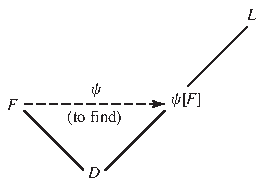
\includegraphics[width=0.359\linewidth,height=.8\textheight,keepaspectratio]{assets/p232_22.pdf}\end{center}
\begin{center}\small\textbf{26.8 Figure}\end{center}
\end{BookFloat}

\end{BookBody}

% Source PDF page 233; original printed page 216
\BookSource{233}{216}
\BookNarrativetrue

\begin{BookBody}

\noindent Every \BookInline{x\in F} is a quotient \BookInline{a/_{F}b} of some two elements \BookInline{a} and \BookInline{b,\allowbreak b\neq 0,\allowbreak } of \BookInline{D.} Let us attempt to define \BookInline{\psi } by

\begin{center}\begin{adjustbox}{max width=\linewidth}\BookInline{\displaystyle \psi (a/_{F}b)= \psi (a)/_{L}\psi (b).}\end{adjustbox}\end{center}

\noindent We must first show that this map \BookInline{\psi } is sensible and well-defined. Since \BookInline{\psi } is the identity on \BookInline{D,\allowbreak } for \BookInline{b\neq 0} we have \BookInline{\psi (b)\neq 0,\allowbreak } so our definition of \BookInline{\psi (a/_{F}b)} as \BookInline{\psi (a)/_{L}\psi (b)} makes sense. If \BookInline{a/_{F}b= c/_{F}d} in \BookInline{F,\allowbreak } then \BookInline{ad= bc} in \BookInline{D,\allowbreak } so \BookInline{\psi (ad)= \psi (bc).} But since \BookInline{\psi } is the identity on \BookInline{D,\allowbreak }

\begin{center}\begin{adjustbox}{max width=\linewidth}\BookInline{\displaystyle \psi (ad)= \psi (a)\psi (d)\;\text{and}\;\psi (bc)= \psi (b)\psi (c).}\end{adjustbox}\end{center}

\noindent Thus

\begin{center}\begin{adjustbox}{max width=\linewidth}\BookInline{\displaystyle \psi (a)/_{L}\psi (b)= \psi (c)/_{L}\psi (d)}\end{adjustbox}\end{center}

\noindent in \BookInline{L,\allowbreak } so \BookInline{\psi } is well-defined.

The equations

\begin{center}\begin{adjustbox}{max width=\linewidth}\BookInline{\displaystyle \psi (xy)= \psi (x)\psi (y)}\end{adjustbox}\end{center}

\noindent and

\begin{center}\begin{adjustbox}{max width=\linewidth}\BookInline{\displaystyle \psi (x+ y)= \psi (x)+ \psi (y)}\end{adjustbox}\end{center}

\noindent follow easily from the definition of \BookInline{\psi } on \BookInline{F} and from the fact that \BookInline{\psi } is the identity on \BookInline{D.}

If \BookInline{\psi (a/_{F}b)= \psi (c/_{F}d),\allowbreak } we have

\begin{center}\begin{adjustbox}{max width=\linewidth}\BookInline{\displaystyle \psi (a)/_{L}\psi (b)= \psi (c)/_{L}\psi (d)}\end{adjustbox}\end{center}

\noindent so

\begin{center}\begin{adjustbox}{max width=\linewidth}\BookInline{\displaystyle \psi (a)\psi (d)= \psi (b)\psi (c).}\end{adjustbox}\end{center}

\noindent Since \BookInline{\psi } is the identity on \BookInline{D,\allowbreak } we then deduce that \BookInline{ad= bc,\allowbreak } so \BookInline{a/_{F}b= c/_{F}d.} Thus \BookInline{\psi } is one-to-one.

By definition\BookInline{,\allowbreak \psi (a)= a} for \BookInline{a\in D.} \BookEnd{\blacklozenge}

\BookLabel{26.9 Corollary} Every field \BookInline{L} containing an integral domain \BookInline{D} contains a field of quotients of \BookInline{D.}

\BookLabel{\textit{Proof}} In the proof of Theorem 26.7 every element of the subfield \BookInline{\psi [F]} of \BookInline{L} is a quotient in \BookInline{L} of elements of \BookInline{D.}\BookEnd{\blacklozenge}

\BookLabel{26.10 Corollary} Any two fields of quotients of an integral domain \BookInline{D} are isomorphic.

\BookLabel{\textit{Proof}} Suppose in Theorem 26.7 that \BookInline{L} is a field of quotients of \BookInline{D,\allowbreak } so that every element \BookInline{x} of \BookInline{L} can be expressed in the form \BookInline{a/_{L}b} for \BookInline{a,\allowbreak b\in D.} Then \BookInline{L} is the field \BookInline{\psi [F]} of the proof of Theorem 26.7 and is thus isomorphic to \BookInline{F.}\BookEnd{\blacklozenge}

\end{BookBody}

\BookNarrativefalse

\begin{BookBody}

\BookExerciseTitle{26}

\BookTextHeading{\textbf{Computations}}

\BookExercise{1.}{Describe the field \BookInline{F} of quotients of the integral subdomain}

\begin{center}\begin{adjustbox}{max width=\linewidth}\BookInline{\displaystyle D= \{n+ mi\mid n,\allowbreak m\in \mathbb{Z}\}}\end{adjustbox}\end{center}

\noindent of \BookInline{\mathbb{C}.} “Describe” means give the elements of \BookInline{\mathbb{C}} that make up the field of quotients of \BookInline{D} in \BookInline{\mathbb{C}.(}The elements of \BookInline{D} are the\textbf{ Gaussian integers.})

\BookExercise{2.}{Describe (in the sense of Exercise 1) the field \BookInline{F} of quotients of the integral subdomain \BookInline{D= \{n+ m\sqrt{3}\mid n,\allowbreak m\in \mathbb{Z}\}} of \BookInline{\mathbb{R}.}}

\end{BookBody}

% Source PDF page 234; original printed page 217
\BookSource{234}{217}
\BookNarrativefalse

\begin{BookBody}

\BookTextHeading{\textbf{Concepts}}

\BookExercise{3.}{Correct the definition of the italicized term without reference to the text, if correction is needed, so that it is in a form acceptable for publication.}

A \BookInline{\text{fi}eld} \textit{of quotients} of an integral domain \BookInline{D} is a field \BookInline{F} in which \BookInline{D} can be embedded so that every nonzero element of \BookInline{D} is a unit in \BookInline{F.}

\BookExercise{4.}{Determine whether each of the following is true or false.}

\BookExercise{a.}{\textbf{a}\BookInline{.\mathbb{Q}} is a field of quotients of \BookInline{\mathbb{Z}.}}

\BookExercise{b.}{\textbf{b}\BookInline{.\mathbb{R}} is a field of quotients of \BookInline{\mathbb{Z}.}}

\BookExercise{c.}{\textbf{c}\BookInline{.\mathbb{R}} is a field of quotients of \BookInline{\mathbb{R}.}}

\BookExercise{d.}{\textbf{d}\BookInline{.\mathbb{C}} is a field of quotients of \BookInline{\mathbb{R}.}}

\BookExercise{e.}{If \BookInline{D} is a field, then any field of quotients of \BookInline{D} is isomorphic to \BookInline{D.}}

\BookExercise{f.}{The fact that \BookInline{D} has no divisors of 0 was used strongly several times in the construction of a field \BookInline{F} of quotients of the integral domain \BookInline{D.}}

\BookExercise{g.}{Every element of an integral domain \BookInline{D} is a unit in a field \BookInline{F} of quotients of \BookInline{D.}}

\BookExercise{h.}{Every nonzero element of an integral domain \BookInline{D} is a unit in a field \BookInline{F} of quotients of \BookInline{D.}}

\BookExercise{i.}{A field of quotients \BookInline{F^{\prime }} of a subdomain \BookInline{D^{\prime }} of an integral domain \BookInline{D} can be regarded as a subfield of some field of quotients of \BookInline{D.}}

\BookExercise{j.}{Every field of quotients of \BookInline{\mathbb{Z}} is isomorphic to \BookInline{\mathbb{Q}.}}

\BookExercise{5.}{Show by an example that a field \BookInline{F^{\prime }} of quotients of a proper subdomain \BookInline{D^{\prime }} of an integral domain \BookInline{D} may also be a field of quotients for \BookInline{D.}}

\BookTextHeading{\textbf{Theory}}

\BookExercise{6.}{Prove Part 2 of Step 3. You may assume any preceding part of Step 3.}

\BookExercise{7.}{Prove Part 3 of Step 3. You may assume any preceding part of Step 3.}

\BookExercise{8.}{Prove Part 4 of Step 3. You may assume any preceding part of Step 3.}

\BookExercise{9.}{Prove Part 5 of Step 3. You may assume any preceding part of Step 3.}

\BookExercise{10.}{Prove Part 6 of Step 3. You may assume any preceding part of Step 3.}

\BookExercise{11.}{Prove Part 7 of Step 3. You may assume any preceding part of Step 3.}

\BookExercise{12.}{Let \BookInline{R} be a nonzero commutative ring, and let \BookInline{T} be a nonempty subset of \BookInline{R} closed under multiplication and containing neither 0 nor divisors of 0. Starting with \BookInline{R\times T} and otherwise exactly following the construction in this section, we can show that the ring \BookInline{R} can be enlarged to a\textit{ partial ring of quotients} \BookInline{Q(R,\allowbreak T).} Think about this for 15 minutes or so; look back over the construction and see why things still work. In particular, show the following:}

\BookExercise{a.}{\textbf{a}\BookInline{.Q(R,\allowbreak T)} has unity even if \BookInline{R} does not.}

\BookExercise{b.}{In \BookInline{Q(R,\allowbreak T),\allowbreak } every nonzero element of \BookInline{T} is a unit.}

\BookExercise{13.}{Prove from Exercise 12 that every nonzero commutative ring containing an element \BookInline{a} that is not a divisor of 0 can be enlarged to a commutative ring with unity. Compare with Exercise 36 of Section 23.}

\BookExercise{14.}{With reference to Exercise 12, how many elements are there in the ring \BookInline{Q(\mathbb{Z}_{4},\allowbreak \{1,\allowbreak 3\})}?}

\BookExercise{15.}{With reference to Exercise 12, describe the ring \BookInline{Q(\mathbb{Z},\allowbreak \{2^{n}\mid n\in \mathbb{Z}^{+ }\}),\allowbreak } by describing a subring of \BookInline{\mathbb{R}} to which it is isomorphic.}

\BookExercise{16.}{With reference to Exercise 12, describe the ring \BookInline{Q(3\mathbb{Z},\allowbreak \{6^{n}\mid n\in \mathbb{Z}^{+ }\})} by describing a subring of \BookInline{\mathbb{R}} to which it is isomorphic.}

\BookExercise{17.}{With reference to Exercise 12, suppose we drop the condition that \BookInline{T} have no divisors of zero and just require that nonempty \BookInline{T} not containing 0 be closed under multiplication. The attempt to enlarge \BookInline{R} to a commutative ring with unity in which every nonzero element of \BookInline{T} is a unit must fail if \BookInline{T} contains an element \BookInline{a} that is a divisor of 0, for a divisor of 0 cannot also be a unit. Try to discover where a construction parallel to that in the text but starting with \BookInline{R\times T} first runs into trouble. In particular, for \BookInline{R= \mathbb{Z}_{6}} and \BookInline{T= \{1,\allowbreak 2,\allowbreak 4\},\allowbreak } illustrate the first difficulty encountered. [\textit{Hint:} It is in Step 1.]}

\end{BookBody}
\ifdefined\BookMaster\let\BookFinish\relax\else\def\BookFinish{\end{document}}\fi\BookFinish

\clearpage
% !TeX program = xelatex
\ifdefined\BookMaster\else
\documentclass[11pt,oneside]{article}
% !TeX program = xelatex
\usepackage[b5paper,left=22mm,right=22mm,top=20mm,bottom=22mm,footskip=11mm]{geometry}
\usepackage{fontspec}
\setmainfont{TeX Gyre Termes}
\setsansfont{TeX Gyre Heros}
\usepackage{amsmath,amssymb,mathtools,amsthm}
\renewcommand{\cdots}{\mathinner{\cdotp\cdotp\cdotp}}
\usepackage{graphicx,adjustbox,array,booktabs,longtable,multirow,enumitem,changepage,needspace}
\usepackage[table]{xcolor}
\usepackage{fancyhdr}
\raggedbottom
\interfootnotelinepenalty=10000
\newcommand{\BookFootnote}[2]{\begingroup\renewcommand{\thefootnote}{\fnsymbol{footnote}}\footnote[#1]{#2}\endgroup}
\newcommand{\BookFootnoteMark}[1]{\begingroup\renewcommand{\thefootnote}{\fnsymbol{footnote}}\footnotemark[#1]\endgroup}
\newcommand{\BookFootnoteText}[2]{\begingroup\renewcommand{\thefootnote}{\fnsymbol{footnote}}\footnotetext[#1]{#2}\endgroup}
\newenvironment{BookFloat}[1]{\par\addvspace{.6\baselineskip}\noindent\def\BookFloatID{#1}\begin{minipage}{\linewidth}\phantomsection\label{bookfloat:#1:start}}{\phantomsection\label{bookfloat:\BookFloatID:end}\end{minipage}\par\addvspace{.6\baselineskip}}

\usepackage[unicode,hidelinks]{hyperref}
\pagestyle{fancy}
\fancyhf{}
\newcommand{\BookFooter}{}
\fancyfoot[L]{\parbox[b]{\dimexpr\textwidth-15mm}{\footnotesize\BookFooter}}
\fancyfoot[R]{\footnotesize\thepage}
\renewcommand{\headrulewidth}{0pt}
\renewcommand{\footrulewidth}{0pt}
\setlength{\parindent}{0pt}
\setlength{\parskip}{0.2em}
\setlength{\emergencystretch}{3em}
\setlist{nosep,leftmargin=1.7em,labelsep=.65em}
\newif\ifBookNarrative
\BookNarrativetrue
\newenvironment{BookBody}{\setlength{\parindent}{0pt}}{}
\newcommand{\BookStatement}[1]{\par\addvspace{.6\baselineskip}\noindent #1\enspace\ignorespaces}
\newcommand{\BookLabel}[1]{\par\addvspace{.6\baselineskip}\needspace{3\baselineskip}\noindent\textbf{#1}\quad\ignorespaces}
\newcommand{\BookHeading}[1]{\par\addvspace{\baselineskip}\needspace{4\baselineskip}\noindent{\large\bfseries #1}\par\medskip}
\newcommand{\BookSubheading}[1]{\par\addvspace{.7\baselineskip}\needspace{3\baselineskip}\noindent{\bfseries #1}\par\smallskip}
\newcommand{\BookTextHeading}[1]{\par\addvspace{.7\baselineskip}\needspace{3\baselineskip}\noindent #1\par\smallskip}
\newcommand{\BookSectionTitle}[2]{\par\addvspace{1.2\baselineskip}\needspace{5\baselineskip}\noindent\colorbox{gray!25}{\sffamily\bfseries\small SECTION #1}\quad{\large\bfseries #2}\par\medskip}
\newcommand{\BookExerciseTitle}[1]{\par\addvspace{\baselineskip}\needspace{4\baselineskip}\noindent{\color{gray}\rule{1.5mm}{1.5mm}}\enspace{\large\bfseries Exercises #1}\par\medskip}
\newcommand{\BookBullet}[1]{\begin{list}{\textbullet}{\setlength{\leftmargin}{1.7em}\setlength{\labelwidth}{1em}\setlength{\labelsep}{.7em}\setlength{\topsep}{0pt}\setlength{\parsep}{0pt}\setlength{\itemsep}{0pt}}\item #1\end{list}}
\newcommand{\BookExercise}[2]{\begin{list}{\textbf{#1}}{\setlength{\leftmargin}{2.2em}\setlength{\labelwidth}{1.5em}\setlength{\labelsep}{.7em}\setlength{\topsep}{.15em}\setlength{\parsep}{0pt}\setlength{\itemsep}{0pt}}\item #2\end{list}}
\newcommand{\BookEnd}[1]{\unskip\nobreak\hfill\ensuremath{#1}}
\newcommand{\BookSource}[2]{\phantomsection\label{sourcepage:#1}} % Source-page anchors, retained through reflow.
\usepackage{multicol}
\usepackage{tikz}
\newcommand{\BookPartEntry}[2]{\par\noindent\makebox[17mm][l]{\bfseries Section #1}#2\par}
\newcommand{\BookPartTitle}[3]{\par\bigskip\noindent\begin{tikzpicture}\node[anchor=north west,inner sep=0pt,outer sep=0pt] (bookpart) at (0,0) {\begin{minipage}{\dimexpr\linewidth-.5pt}\hspace*{26mm}\begin{minipage}[t]{\dimexpr\linewidth-26mm}\begin{adjustbox}{max width=\linewidth}{\fontsize{20}{24}\selectfont\bfseries #2}\end{adjustbox}\par\vspace{6mm}\hrule\vspace{6mm}{\sffamily\footnotesize\setlength{\parskip}{.3em}#3}\vspace{3mm}\end{minipage}\end{minipage}};\path[shade,top color=gray!60,bottom color=white] (0,0) rectangle ([xshift=24mm]bookpart.south west);\node[anchor=north,font=\sffamily\bfseries\small] at (12mm,-2mm) {PART};\node[anchor=north,font=\sffamily\bfseries\Huge] at (12mm,-7mm) {#1};\end{tikzpicture}\par\bigskip}
\newsavebox{\BookMathBox}
\makeatletter
\newcommand{\BookInline}[1]{\leavevmode\hskip0pt\relax\begingroup\in@{\begin}{#1}\ifin@\sbox{\BookMathBox}{\(#1\)}\ifdim\wd\BookMathBox>\dimexpr\linewidth-1em\relax\resizebox{\dimexpr\linewidth-1em\relax}{!}{\usebox{\BookMathBox}}\else\(#1\)\fi\else\in@{\left}{#1}\ifin@\sbox{\BookMathBox}{\(#1\)}\ifdim\wd\BookMathBox>\dimexpr\linewidth-1em\relax\resizebox{\dimexpr\linewidth-1em\relax}{!}{\usebox{\BookMathBox}}\else\(#1\)\fi\else\(#1\)\fi\fi\endgroup\hskip0pt\relax}
\makeatother
\DeclareMathOperator{\Aut}{Aut}
\DeclareMathOperator{\End}{End}
\DeclareMathOperator{\Hom}{Hom}
\DeclareMathOperator{\GF}{GF}
\DeclareMathOperator{\irr}{irr}
\DeclareMathOperator{\lt}{lt}
\DeclareMathOperator{\lp}{lp}
\providecommand{\textcircled}[1]{\textnormal{(#1)}}

\begin{document}
\fi
\renewcommand{\BookFooter}{Section 27 Rings of Polynomials}
\pdfbookmark[0]{Section 27 Rings of Polynomials}{27_rings_of_polynomials}
\ifdefined\BookMaster\else\setcounter{page}{218}\fi
% Source PDF page 235; original printed page 218
\BookSource{235}{218}
\BookNarrativetrue

\begin{BookBody}

\BookSectionTitle{27}{Rings of Polynomials}

\BookTextHeading{\textbf{Polynomials in an Indeterminate}  }

\noindent We all have a pretty workable idea of what constitutes a\textit{ polynomial in} \BookInline{x} \textit{with coefficients} \textit{in} \BookInline{a} \textit{ring} \BookInline{R.} We can guess how to add and multiply such polynomials and know what is meant by the\textit{ degree} of a polynomial. We expect that the set \BookInline{R[x]} of all polynomials with coefficients in the ring \BookInline{R} is itself a ring with the usual operations of polynomial addition and multiplication, and that \BookInline{R} is a subring of \BookInline{R[x].} However, we will be working with polynomials from a slightly different viewpoint than the approach in high school algebra or calculus, and there are a few things that we want to say.

In the first place, we will call \BookInline{x} an\textbf{ indeterminate} rather than a variable. Suppose, for example that our ring of coefficients is \BookInline{\mathbb{Z}.} One of the polynomials in the ring \BookInline{\mathbb{Z}[x]} is \BookInline{1x,\allowbreak } which we shall write simply as \BookInline{x.} Now \BookInline{x} is not 1 or 2 or any of the other elements of \BookInline{\mathbb{Z}[x].} Thus from now on we will never write such things as “\BookInline{x= 1}” or “\BookInline{x= 2,\allowbreak }” as we have done in other courses. We call \BookInline{x} an indeterminate rather than a variable to emphasize this change. Also, we will never write an expression such as “\BookInline{x^{2}- 4= 0,\allowbreak }” simply because \BookInline{x^{2}- 4} is not the zero polynomial in our ring \BookInline{\mathbb{Z}[x].} We are accustomed to speaking of “solving a polynomial equation,” and will be spending a lot of time in the remainder of our text discussing this, but we will always refer to it as “finding a zero of a polynomial.” In summary, we try to be careful in our discussion of algebraic structures not to say in one context that things are equal and in another context that they are not equal.

If a person knows nothing about polynomials, it is not an easy task to describe precisely the nature of a polynomial in \BookInline{x} with coefficients in a ring \BookInline{R.} If we just define such a polynomial to be a\textit{ finite formal sum}

\begin{center}\begin{adjustbox}{max width=\linewidth}\BookInline{\displaystyle \sum _{i= 0}^{n}a_{i}x^{i}= a_{0}+ a_{1}x+ \cdots + a_{n}x^{n},\allowbreak }\end{adjustbox}\end{center}

\BookTextHeading{\ensuremath{\blacksquare} \textbf{HISTORICAL NOTE}  }

\noindent The use of \BookInline{x} and other letters near the end of the alphabet to represent an “indeterminate” is due to Rene´ Descartes (1596–1650). Earlier, Franc¸ois Viete (1540–1603) had used vowels for indeterminates and consonants for known quantities. Descartes is also responsible for the first publication of the factor theorem (Corollary 28.4) in his work\textit{ The Geometry,} which appeared as an appendix to his\textit{ Discourse on Method} (1637). This work also contained the first publication of the basic concepts of analytic geometry; Descartes showed how geometric curves can be described algebraically.

to reject as absolutely false everything of which he had the least doubt; but, since it was necessary that he who was thinking was “something,” he conceived his first principle of philosophy: “I think, therefore I am.” The most enlightening parts of the\textit{ Discourse on Method,} however, are the three appendices:\textit{ The Optics, The Geometry,} and\textit{ The Meteorology}. It was here that Descartes provided examples of how he actually applied his method. Among the important ideas Descartes discovered and published in these works were the sine law of refraction of light, the basics of the theory of equations, and a geometric explanation of the rainbow.

\noindent Descartes was born to a wealthy family in La Haye, France; since he was always of delicate health, he formed the habit of spending his mornings in bed. It was at these times that he accomplished his most productive work. The\textit{ Dis}\textit{course on Method} was Descartes’ attempt to show the proper procedures for “searching for truth in the sciences.” The first step in this process was

In 1649, Descartes was invited by Queen Christina of Sweden to come to Stockholm to tutor her. Unfortunately, the Queen required him, contrary to his long-established habits, to rise at an early hour. He soon contracted a lung disease and died in 1650.

\end{BookBody}

% Source PDF page 236; original printed page 219
\BookSource{236}{219}
\BookNarrativetrue

\begin{BookBody}

\noindent where \BookInline{a_{i}\in R,\allowbreak } we get ourselves into a bit of trouble. For surely \BookInline{0+ a_{1}x} and \BookInline{0+ a_{1}x+ } \BookInline{0x^{2}} are different as formal sums, but we want to regard them as the same polynomial. A practical solution to this problem is to define a polynomial as an\textit{ infinite formal sum}

\begin{center}\begin{adjustbox}{max width=\linewidth}\BookInline{\displaystyle \sum _{i= 0}^{\infty }a_{i}x^{i}= a_{0}+ a_{1}x+ \cdots + a_{n}x^{n}+ \cdots ,\allowbreak }\end{adjustbox}\end{center}

\noindent where \BookInline{a_{i}= 0} for all but a finite number of values of \BookInline{i.} Now there is no problem of having more than one finite formal sum represent what we wish to consider a single polynomial.

\BookLabel{27.1 Definition} Let \BookInline{R} be a ring. A\textbf{ polynomial} \BookInline{f(x)} \textbf{with coefficients in} \BookInline{R} is an infinite formal sum

\begin{center}\begin{adjustbox}{max width=\linewidth}\BookInline{\displaystyle \sum _{i= 0}^{\infty }a_{i}x^{i}= a_{0}+ a_{1}x+ \cdots + a_{n}x^{n}+ \cdots ,\allowbreak }\end{adjustbox}\end{center}

\noindent where \BookInline{a_{i}\in R} and for all but a finite number of values of \BookInline{i,\allowbreak a_{i}= 0.} The \BookInline{a_{i}} are\textbf{ coefficients} \textbf{of} \BookInline{f(x).} If for some \BookInline{i\geq 0} it is true that \BookInline{a_{i}\neq 0,\allowbreak } the largest such value of \BookInline{i} is the\textbf{ degree} \textbf{of} \BookInline{f(x).} If all \BookInline{a_{i}= 0,\allowbreak } then the degree of \BookInline{f(x)} is undefined.\label{bookfootnote:236:2:ref}\BookFootnote{2}{\label{bookfootnote:236:2:text}The degree of the zero polynomial is sometimes defined to be \BookInline{- 1,\allowbreak } which is the first integer less than 0, or defined to be \BookInline{- \infty } so that the degree of \BookInline{f(x)g(x)} will be the sum of the degrees of \BookInline{f(x)} and \BookInline{g(x)} if one of them is zero.} \BookEnd{\blacksquare}

To simplify working with polynomials, let us agree that if \BookInline{f(x)= a_{0}+ a_{1}x+ \cdots + } \BookInline{a_{n}x^{n}+ \cdots } has \BookInline{a_{i}= 0} for \BookInline{i>n,\allowbreak } then we may denote \BookInline{f(x)} by \BookInline{a_{0}+ a_{1}x+ \cdots + a_{n}x^{n}.} Also, if \BookInline{R} has unity \BookInline{1\neq 0,\allowbreak } we will write a term \BookInline{1x^{k}} in such a sum as \BookInline{x^{k}.} For example, in \BookInline{\mathbb{Z}[x],\allowbreak } we will write the polynomial \BookInline{2+ 1x} as \BookInline{2+ x.} Finally, we shall agree that we may omit altogether from the formal sum any term \BookInline{0x^{i},\allowbreak } or \BookInline{a_{0}} if \BookInline{a_{0}= 0} but not all \BookInline{a_{i}= 0.} Thus \BookInline{0,\allowbreak 2,\allowbreak x,\allowbreak } and \BookInline{2+ x^{2}} are polynomials with coefficients in \BookInline{\mathbb{Z}.} An element of \BookInline{R} is a \textbf{constant polynomial.}

Addition and multiplication of polynomials with coefficients in a ring \BookInline{R} are defined in a way familiar to us. If

\begin{center}\begin{adjustbox}{max width=\linewidth}\BookInline{\displaystyle f(x)= a_{0}+ a_{1}x+ \cdots + a_{n}x^{n}+ \cdots}\end{adjustbox}\end{center}

\noindent and

\begin{center}\begin{adjustbox}{max width=\linewidth}\BookInline{\displaystyle g(x)= b_{0}+ b_{1}x+ \cdots + b_{n}x^{n}+ \cdots ,\allowbreak }\end{adjustbox}\end{center}

\noindent then for polynomial addition, we have

\begin{center}\begin{adjustbox}{max width=\linewidth}\BookInline{\displaystyle f(x)+ g(x)= c_{0}+ c_{1}x+ \cdots + c_{n}x^{n}+ \cdots \;\text{where}\;c_{n}= a_{n}+ b_{n},\allowbreak }\end{adjustbox}\end{center}

\noindent and for polynomial multiplication, we have

\begin{center}\begin{adjustbox}{max width=\linewidth}\BookInline{\displaystyle f(x)g(x)= d_{0}+ d_{1}x+ \cdots + d_{n}x^{n}+ \cdots \;\text{where}\;d_{n}= \sum _{i= 0}^{n}a_{i}b_{n- i}}\end{adjustbox}\end{center}

\noindent Observe that both \BookInline{c_{i}} and \BookInline{d_{i}} are 0 for all but a finite number of values of \BookInline{i,\allowbreak } so these definitions make sense. Note that \BookInline{\sum _{i= 0}^{n}a_{i}b_{n- i}} need not equal \BookInline{\sum _{i= 0}^{n}b_{i}a_{n- i}} if \BookInline{R} is not commutative. With these definitions of addition and multiplication, we have the following theorem.

\BookLabel{27.2 Theorem} The set \BookInline{R[x]} of all polynomials in an indeterminate \BookInline{x} with coefficients in a ring \BookInline{R} is a ring under polynomial addition and multiplication. If \BookInline{R} is commutative, then so is \BookInline{R[x],\allowbreak } and if \BookInline{R} has unity \BookInline{1\neq 0,\allowbreak } then 1 is also unity for \BookInline{R[x].}

\BookLabel{\textit{Proof}} That \BookInline{\langle R[x],\allowbreak + \rangle } is an abelian group is apparent. The associative law for multiplication and the distributive laws are straightforward, but slightly cumbersome, computations. We illustrate by proving the associative law.

\end{BookBody}

% Source PDF page 237; original printed page 220
\BookSource{237}{220}
\BookNarrativetrue

\begin{BookBody}

Applying ring axioms to \BookInline{a_{i},\allowbreak b_{j},\allowbreak c_{k}\in R,\allowbreak } we obtain

\begin{center}\begin{adjustbox}{max width=\linewidth}\BookInline{\displaystyle \begin{aligned}\Bigg[\Bigg(\sum_{i=0}^{\infty} a_i x^i\Bigg)\Bigg(\sum_{j=0}^{\infty} b_j x^j\Bigg)\Bigg]\Bigg(\sum_{k=0}^{\infty} c_k x^k\Bigg)&= \Bigg[\sum_{n=0}^{\infty} \Bigg(\sum_{i=0}^{n} a_i b_{n-i}\Bigg)x^n\Bigg]\Bigg(\sum_{k=0}^{\infty} c_k x^k\Bigg)\\&= \sum_{s=0}^{\infty} \Bigg[\sum_{n=0}^{s} \Bigg(\sum_{i=0}^{n} a_i b_{n-i}\Bigg)c_{s-n}\Bigg]x^s\\&= \sum_{s=0}^{\infty} \Bigg(\sum_{i+j+k=s} a_i b_j c_k\Bigg)x^s\\&= \sum_{s=0}^{\infty} \Bigg[\sum_{m=0}^{s} a_{s-m}\Bigg(\sum_{j=0}^{m} b_j c_{m-j}\Bigg)\Bigg]x^s\\&= \Bigg(\sum_{i=0}^{\infty} a_i x^i\Bigg)\Bigg[\sum_{m=0}^{\infty} \Bigg(\sum_{j=0}^{m} b_j c_{m-j}\Bigg)x^m\Bigg]\\&= \Bigg(\sum_{i=0}^{\infty} a_i x^i\Bigg)\Bigg[\Bigg(\sum_{j=0}^{\infty} b_j x^j\Bigg)\Bigg(\sum_{k=0}^{\infty} c_k x^k\Bigg)\Bigg].\end{aligned}}\end{adjustbox}\end{center}

Whew! In this computation, the fourth expression, having just two summation signs, should be viewed as the value of the triple product \BookInline{f(x)g(x)h(x)} of these polynomials under this associative multiplication. (In a similar fashion, we view \BookInline{f(g(h(x)))} as the value of the associative composition \BookInline{(f\circ g\circ h)(x)} of three functions \BookInline{f,\allowbreak g,\allowbreak } and \BookInline{h.)}

The distributive laws are similarly proved. (See Exercise 26.)

The comments prior to the statement of the theorem show that \BookInline{R[x]} is a commutative ring if \BookInline{R} is commutative, and a unity \BookInline{1\neq 0} in \BookInline{R} is also unity for \BookInline{R[x],\allowbreak } in view of the definition of multiplication in \BookInline{R[x].}\BookEnd{\blacklozenge}

Thus \BookInline{\mathbb{Z}[x]} is the ring of polynomials in the indeterminate \BookInline{x} with integral coefficients\BookInline{,\allowbreak \mathbb{Q}[x]} the ring of polynomials in \BookInline{x} with rational coefficients, and so on.

\BookLabel{27.3 Example} In \BookInline{\mathbb{Z}_{2}[x],\allowbreak } we have

\begin{center}\begin{adjustbox}{max width=\linewidth}\BookInline{\displaystyle (x+ 1)^{2}= (x+ 1)(x+ 1)= x^{2}+ (1+ 1)x+ 1= x^{2}+ 1.}\end{adjustbox}\end{center}

\noindent Still working in \BookInline{\mathbb{Z}_{2}[x],\allowbreak } we obtain

\begin{center}\begin{adjustbox}{max width=\linewidth}\BookInline{\displaystyle (x+ 1)+ (x+ 1)= (1+ 1)x+ (1+ 1)= 0x+ 0= 0.}\end{adjustbox}\end{center} \BookEnd{\blacktriangle}

If \BookInline{R} is a ring and \BookInline{x} and \BookInline{y} are two indeterminates, then we can form the ring \BookInline{(R[x])[y],\allowbreak } that is, the ring of polynomials in \BookInline{y} with coefficients that are polynomials in \BookInline{x.} Every polynomial in \BookInline{y} with coefficients that are polynomials in \BookInline{x} can be rewritten in a natural way as a polynomial in \BookInline{x} with coefficients that are polynomials in \BookInline{y} as illustrated by Exercise 20. This indicates that \BookInline{(R[x])[y]} is naturally isomorphic to \BookInline{(R[y])[x],\allowbreak } although a careful proof is tedious. We shall identify these rings by means of this natural isomorphism, and shall consider this ring \BookInline{R[x,\allowbreak y]} the\textbf{ ring of polynomials in two inde}\textbf{terminates} \BookInline{x} \textbf{and} \BookInline{y} \textbf{with coefficients in} \BookInline{R.} The\textbf{ ring} \BookInline{R[x_{1},\allowbreak \cdots,\allowbreak x_{n}]} \textbf{of polynomials in} \textbf{the} \BookInline{n} \textbf{indeterminates} \BookInline{x_{i}} \textbf{with coefficients in} \BookInline{R} is similarly defined.

We leave as Exercise 24 the proof that if \BookInline{D} is an integral domain, then so is \BookInline{D[x].} In particular, if \BookInline{F} is a field, then \BookInline{F[x]} is an integral domain. Note that \BookInline{F[x]} is not a field, for \BookInline{x} is not a unit in \BookInline{F[x].} That is, there is no polynomial \BookInline{f(x)\in F[x]} such that \BookInline{xf(x)= 1.} By Theorem 26.6, one can construct the field of quotients \BookInline{F(x)} of \BookInline{F[x].} Any element in \BookInline{F(x)} can be represented as a quotient \BookInline{f(x)/g(x)} of two polynomials in \BookInline{F[x]} with

\end{BookBody}

% Source PDF page 238; original printed page 221
\BookSource{238}{221}
\BookNarrativetrue

\begin{BookBody}

\noindent \BookInline{g(x)\neq 0.} We similarly define \BookInline{F(x_{1},\allowbreak \cdots,\allowbreak x_{n})} to be the field of quotients of \BookInline{F[x_{1},\allowbreak \cdots,\allowbreak x_{n}].} This field \BookInline{F(x_{1},\allowbreak \cdots,\allowbreak x_{n})} is the\textbf{ field of rational functions in} \BookInline{n} \textbf{indeterminates over} \BookInline{F.} These fields play a very important role in algebraic geometry.

\BookTextHeading{\textbf{The Evaluation Homomorphisms}  }

\noindent We are now ready to proceed to show how homomorphisms can be used to study what we have always referred to as “solving a polynomial equation.” Let \BookInline{E} and \BookInline{F} be fields, with \BookInline{F} a subfield of \BookInline{E,\allowbreak } that is\BookInline{,\allowbreak F\leq E.} The next theorem asserts the existence of very important homomorphisms of \BookInline{F[x]} into \BookInline{E.} \textit{These homomorphisms will be the fundamental} \textit{tools for much of the rest of our work}.

\BookLabel{27.4 Theorem} \textbf{(The Evaluation Homomorphisms for Field Theory)} Let \BookInline{F} be a subfield of a field \BookInline{E,\allowbreak } let \BookInline{\alpha } be any element of \BookInline{E,\allowbreak } and let \BookInline{x} be an indeterminate. The map \BookInline{\phi _{\alpha }:F[x]\to E} defined by

\begin{center}\begin{adjustbox}{max width=\linewidth}\BookInline{\displaystyle \phi _{\alpha }\Big(a_{0}+ a_{1}x+ \cdots + a_{n}x^{n}\Big)= a_{0}+ a_{1}\alpha + \cdots + a_{n}\alpha ^{n}}\end{adjustbox}\end{center}

\noindent for \BookInline{(a_{0}+ a_{1}x+ \cdots + a_{n}x^{n})\in F[x]} is a homomorphism of \BookInline{F[x]} into \BookInline{E.} Also\BookInline{,\allowbreak \phi _{\alpha }(x)= \alpha,\allowbreak } and \BookInline{\phi _{\alpha }} maps \BookInline{F} isomorphically by the identity map; that is\BookInline{,\allowbreak \phi _{\alpha }(a)= a} for \BookInline{a\in F.} The homomorphism \BookInline{\phi _{\alpha }} is\textbf{ evaluation at} \BookInline{\alpha.}

\BookLabel{\textit{Proof}} The subfield and mapping diagram in Fig. 27.5 may help us to visualize this situation. The dashed lines indicate an element of the set. The theorem is really an immediate consequence of our definitions of addition and multiplication in \BookInline{F[x].} The map \BookInline{\phi _{\alpha }} is well defined, that is, independent of our representation of \BookInline{f(x)\in F[x]} as a finite sum

\begin{center}\begin{adjustbox}{max width=\linewidth}\BookInline{\displaystyle a_{0}+ a_{1}x+ \cdots + a_{n}x^{n},\allowbreak }\end{adjustbox}\end{center}

\noindent since such a finite sum representing \BookInline{f(x)} can be changed only by insertion or deletion of terms \BookInline{0x^{i},\allowbreak } which does not affect the value of \BookInline{\phi _{\alpha }(f(x)).}

If \BookInline{f(x)= a_{0}+ a_{1}x+ \cdots + a_{n}x^{n},\allowbreak g(x)= b_{0}+ b_{1}x+ \cdots + b_{m}x^{m},\allowbreak } and \BookInline{h(x)= f(x)+ } \BookInline{g(x)= c_{0}+ c_{1}x+ \cdots + c_{r}x^{r},\allowbreak } then

\begin{center}\begin{adjustbox}{max width=\linewidth}\BookInline{\displaystyle \phi _{\alpha }(f(x)+ g(x))= \phi _{\alpha }(h(x))= c_{0}+ c_{1}\alpha + \cdots + c_{r}\alpha ^{r},\allowbreak }\end{adjustbox}\end{center}

\noindent while

\begin{center}\begin{adjustbox}{max width=\linewidth}\BookInline{\displaystyle \phi _{\alpha }(f(x))+ \phi _{\alpha }(g(x))= \Big(a_{0}+ a_{1}\alpha + \cdots + a_{n}\alpha ^{n}\Big)+ \Big(b_{0}+ b_{1}\alpha + \cdots + b_{m}\alpha ^{m}\Big).}\end{adjustbox}\end{center}

\noindent Since by definition of polynomial addition we have \BookInline{c_{i}= a_{i}+ b_{i},\allowbreak } we see that

\begin{center}\begin{adjustbox}{max width=\linewidth}\BookInline{\displaystyle \phi _{\alpha }(f(x)+ g(x))= \phi _{\alpha }(f(x))+ \phi _{\alpha }(g(x)).}\end{adjustbox}\end{center}

\begin{BookFloat}{27_rings_of_polynomials-p238-15}
\begin{center}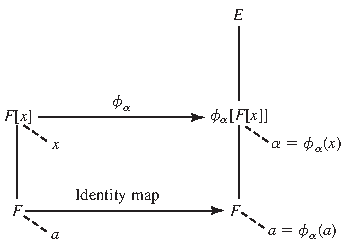
\includegraphics[width=0.473\linewidth,height=.8\textheight,keepaspectratio]{assets/p238_17.pdf}\end{center}
\begin{center}\small\textbf{27.5 Figure}\end{center}
\end{BookFloat}

\end{BookBody}

% Source PDF page 239; original printed page 222
\BookSource{239}{222}
\BookNarrativetrue

\begin{BookBody}

Turning to multiplication, we see that if

\begin{center}\begin{adjustbox}{max width=\linewidth}\BookInline{\displaystyle f(x)g(x)= d_{0}+ d_{1}x+ \cdots + d_{s}x^{s},\allowbreak }\end{adjustbox}\end{center}

\noindent then

\begin{center}\begin{adjustbox}{max width=\linewidth}\BookInline{\displaystyle \phi _{\alpha }(f(x)g(x))= d_{0}+ d_{1}\alpha + \cdots + d_{s}\alpha ^{s},\allowbreak }\end{adjustbox}\end{center}

\noindent while

\begin{center}\begin{adjustbox}{max width=\linewidth}\BookInline{\displaystyle [\phi _{\alpha }(f(x))][\phi _{\alpha }(g(x))]= \Big(a_{0}+ a_{1}\alpha + \cdots + \alpha _{n}\alpha ^{n}\Big)\Big(b_{0}+ b_{1}\alpha + \cdots + b_{m}\alpha ^{m}\Big).}\end{adjustbox}\end{center}

\noindent Since by definition of polynomial multiplication \BookInline{d_{j}= \sum _{i= 0}^{j}a_{i}b_{j- i},\allowbreak } we see that

\begin{center}\begin{adjustbox}{max width=\linewidth}\BookInline{\displaystyle \phi _{\alpha }(f(x)g(x))= [\phi _{\alpha }(f(x))][\phi _{\alpha }(g(x))].}\end{adjustbox}\end{center}

\noindent Thus \BookInline{\phi _{\alpha }} is a homomorphism.

The very definition of \BookInline{\phi _{\alpha }} applied to a constant polynomial \BookInline{a\in F[x],\allowbreak } where \BookInline{a\in F,\allowbreak } gives \BookInline{\phi _{\alpha }(a)= a,\allowbreak } so \BookInline{\phi _{\alpha }} maps \BookInline{F} isomorphically by the identity map. Again by definition of \BookInline{\phi _{\alpha },\allowbreak } we have \BookInline{\phi _{\alpha }(x)= \phi _{\alpha }(1x)= 1\alpha = \alpha.}\BookEnd{\blacklozenge}

We point out that this theorem is valid with the identical proof if \BookInline{F} and \BookInline{E} are merely commutative rings with unity rather than fields. However, we shall be interested primarily in the case in which they are fields.

It is hard to overemphasize the importance of this simple theorem for us. It is the very foundation for all of our further work in field theory. It is so simple that it could justifiably be called an\textit{ observation} rather than a theorem. It was perhaps a little misleading to write out the proof because the polynomial notation makes it look so complicated that you may be fooled into thinking it is a difficult theorem.

\BookLabel{27.6 Example} Let \BookInline{F} be \BookInline{\mathbb{Q}} and \BookInline{E} be \BookInline{\mathbb{R}} in Theorem 27.4, and consider the evaluation homomorphism \BookInline{\phi _{0}:\mathbb{Q}[x]\to \mathbb{R}.} Here

\begin{center}\begin{adjustbox}{max width=\linewidth}\BookInline{\displaystyle \phi _{0}\Big(a_{0}+ a_{1}x+ \cdots + a_{n}x^{n}\Big)= a_{0}+ a_{1}0+ \cdots + a_{n}0^{n}= a_{0}.}\end{adjustbox}\end{center}

\noindent Thus every polynomial is mapped onto its constant term. \BookEnd{\blacktriangle}

\BookLabel{27.7 Example} Let \BookInline{F} be \BookInline{\mathbb{Q}} and \BookInline{E} be \BookInline{\mathbb{R}} in Theorem 27.4 and consider the evaluation homomorphism \BookInline{\phi _{2}:\mathbb{Q}[x]\to \mathbb{R}.} Here

\begin{center}\begin{adjustbox}{max width=\linewidth}\BookInline{\displaystyle \phi _{2}\Big(a_{0}+ a_{1}x+ \cdots + a_{n}x^{n}\Big)= a_{0}+ a_{1}2+ \cdots + a_{n}2^{n}.}\end{adjustbox}\end{center}

\noindent Note that

\begin{center}\begin{adjustbox}{max width=\linewidth}\BookInline{\displaystyle \phi _{2}(x^{2}+ x- 6)= 2^{2}+ 2- 6= 0.}\end{adjustbox}\end{center}

\noindent Thus \BookInline{x^{2}+ x- 6} is in the kernel \BookInline{N} of \BookInline{\phi _{2}.} Of course,

\begin{center}\begin{adjustbox}{max width=\linewidth}\BookInline{\displaystyle x^{2}+ x- 6= (x- 2)(x+ 3),\allowbreak }\end{adjustbox}\end{center}

\noindent and the reason that \BookInline{\phi _{2}(x^{2}+ x- 6)= 0} is that \BookInline{\phi _{2}(x- 2)= 2- 2= 0.} \BookEnd{\blacktriangle}

\BookLabel{27.8 Example} Let \BookInline{F} be \BookInline{\mathbb{Q}} and \BookInline{E} be \BookInline{\mathbb{C}} in Theorem 27.4 and consider the evaluation homomorphism \BookInline{\phi _{i}:\mathbb{Q}[x]\to \mathbb{C}.} Here

\begin{center}\begin{adjustbox}{max width=\linewidth}\BookInline{\displaystyle \phi _{i}\Big(a_{0}+ a_{1}x+ \cdots + a_{n}x^{n}\Big)= a_{0}+ a_{1}i+ \cdots + a_{n}i^{n}}\end{adjustbox}\end{center}

\noindent and \BookInline{\phi _{i}(x)= i.} Note that

\begin{center}\begin{adjustbox}{max width=\linewidth}\BookInline{\displaystyle \phi _{i}(x^{2}+ 1)= i^{2}+ 1= 0,\allowbreak }\end{adjustbox}\end{center}

\noindent so \BookInline{x^{2}+ 1} is in the kernel \BookInline{N} of \BookInline{\phi _{i}.} \BookEnd{\blacktriangle}

\end{BookBody}

% Source PDF page 240; original printed page 223
\BookSource{240}{223}
\BookNarrativetrue

\begin{BookBody}

\BookLabel{27.9 Example} Let \BookInline{F} be \BookInline{\mathbb{Q}} and let \BookInline{E} be \BookInline{\mathbb{R}} in Theorem 27.4 and consider the evaluation homomorphism \BookInline{\phi _{\pi }:\mathbb{Q}[x]\to \mathbb{R}.} Here

\begin{center}\begin{adjustbox}{max width=\linewidth}\BookInline{\displaystyle \phi _{\pi }\Big(a_{0}+ a_{1}x+ \cdots + a_{n}x^{n}\Big)= a_{0}+ a_{1}\pi + \cdots + a_{n}\pi ^{n}.}\end{adjustbox}\end{center}

\noindent It can be proved that \BookInline{a_{0}+ a_{1}\pi + \cdots + a_{n}\pi ^{n}= 0} if and only if \BookInline{a_{i}= 0} for \BookInline{i= 0,\allowbreak 1,\allowbreak \cdots,\allowbreak n.} Thus the kernel of \BookInline{\phi _{\pi }} is \BookInline{\{0\},\allowbreak } and \BookInline{\phi _{\pi }} is a one-to-one map. This shows that all\textit{ formal} \textit{polynomials in} \BookInline{\pi } \textit{with rational coefficients} form a ring isomorphic to \BookInline{\mathbb{Q}[x]} in a natural way with \BookInline{\phi _{\pi }(x)= \pi.}\BookEnd{\blacktriangle}

\BookTextHeading{\textbf{The New Approach}  }

\noindent We now complete the connection between our new ideas and the classical concept of solving a polynomial equation. Rather than speak of\textit{ solving} \BookInline{a} \textit{polynomial equation,} we shall refer to\textit{ finding} \BookInline{a} \textit{zero of} \BookInline{a} \textit{polynomial}.

\BookLabel{27.10 Definition} Let \BookInline{F} be a subfield of a field \BookInline{E,\allowbreak } and let \BookInline{\alpha } be an element of \BookInline{E.} Let \BookInline{f(x)= a_{0}+ } \BookInline{a_{1}x+ \cdots + a_{n}x^{n}} be in \BookInline{F[x],\allowbreak } and let \BookInline{\phi _{\alpha }:F[x]\to E} be the evaluation homomorphism of Theorem 27.4. Let \BookInline{f(\alpha )} denote

\begin{center}\begin{adjustbox}{max width=\linewidth}\BookInline{\displaystyle \phi _{\alpha }(f(x))= a_{0}+ a_{1}\alpha + \cdots + a_{n}\alpha ^{n}.}\end{adjustbox}\end{center}

\noindent If \BookInline{f(\alpha )= 0,\allowbreak } then \BookInline{\alpha } is a\textbf{ zero of} \BookInline{f(x).} \BookEnd{\blacksquare}

In terms of this definition, we can rephrase the classical problem of finding all real numbers \BookInline{r} such that \BookInline{r^{2}+ r- 6= 0} by letting \BookInline{F= \mathbb{Q}} and \BookInline{E= \mathbb{R}} and\textit{ finding all} \BookInline{\alpha \in \mathbb{R}} \textit{such that}

\begin{center}\begin{adjustbox}{max width=\linewidth}\BookInline{\displaystyle \phi _{\alpha }(x^{2}+ x- 6)= 0,\allowbreak }\end{adjustbox}\end{center}

\noindent \textit{that is, finding all zeros of} \BookInline{x^{2}+ x- 6} in \BookInline{\mathbb{R}.} Both problems have the same answer, since

\begin{center}\begin{adjustbox}{max width=\linewidth}\BookInline{\displaystyle \{\alpha \in \mathbb{R}\mid \phi _{\alpha }(x^{2}+ x- 6)= 0\}= \{r\in \mathbb{R}\mid r^{2}+ r- 6= 0\}= \{2,\allowbreak - 3\}.}\end{adjustbox}\end{center}

It may seem that we have merely succeeded in making a simple problem seem quite complicated. In fact,\textit{ what we have done is to phrase the problem in the language} \textit{of mappings, and we can now use all the mapping machinery that we have developed} \textit{and will continue to develop for its solution}.

\BookTextHeading{\textbf{Our Basic Goal}  }

\noindent We continue to attempt to put our future work in perspective. Sections 30 and 31 are concerned with topics in ring theory that are analogous to the material on factor groups and homomorphisms for group theory. However, our aim in developing these analogous concepts for rings will be quite different from our aims in group theory. In group theory we used the concepts of factor groups and homomorphisms to study the structure of a given group and to determine the types of group structures of certain orders that could exist. We will be talking about homomorphisms and factor rings in Section 30 with an eye to finding zeros of polynomials, which is one of the oldest and most fundamental problems in algebra. Let us take a moment to talk about this aim in the light of mathematical history, using the language of “solving polynomial equations” to which we are accustomed.

We start with the Pythagorean school of mathematics of about 525 B.C. The Pythagoreans worked with the assumption that all distances are\textbf{ commensurable}; that is, given distances \BookInline{a} and \BookInline{b,\allowbreak } there should exist a unit of distance \BookInline{u} and integers \BookInline{n} and \BookInline{m} such that \BookInline{a= (n)(u)} and \BookInline{b= (m)(u).} In terms of numbers, then, thinking of \BookInline{u} as being 
% Source PDF page 241; original printed page 224
\BookSource{241}{224}
one unit of distance, they maintained that all numbers are integers. This idea of commensurability can be rephrased according to our ideas as an assertion that all numbers are rational, for if \BookInline{a} and \BookInline{b} are rational numbers, then each is an integral multiple of the reciprocal of the least common multiple of their denominators. For example, if \BookInline{a= \frac{7}{12}} and \BookInline{b= \frac{19}{15},\allowbreak } then \BookInline{a= (35)(\frac{1}{60})} and \BookInline{b= (76)(\frac{1}{60}).}

\end{BookBody}

\BookNarrativetrue

\begin{BookBody}

The Pythagoreans knew, of course, what is now called the\textit{ Pythagorean theorem;} that is, for a right triangle with legs of lengths \BookInline{a} and \BookInline{b} and a hypotenuse of length \BookInline{c,\allowbreak }

\begin{center}\begin{adjustbox}{max width=\linewidth}\BookInline{\displaystyle a^{2}+ b^{2}= c^{2}.}\end{adjustbox}\end{center}

\noindent They also had to grant the existence of a hypotenuse of a right triangle having two legs of equal length, say one unit each. The hypotenuse of such a right triangle would, as we know, have to have a length of \BookInline{\sqrt{2}.} Imagine then their consternation and dismay when one of their society—according to some stories it was Pythagoras himself— came up with the embarrassing fact that is stated in our terminology in the following theorem.

\BookLabel{27.11 Theorem} The polynomial \BookInline{x^{2}- 2} has no zeros in the rational numbers. Thus \BookInline{\sqrt{2}} is not a rational number.

\BookLabel{\textit{Proof}} Suppose that \BookInline{m/n} for \BookInline{m,\allowbreak n\in \mathbb{Z}} is a rational number such that \BookInline{(m/n)^{2}= 2.} We assume that we have canceled any factors common to \BookInline{m} and \BookInline{n,\allowbreak } so that the fraction \BookInline{m/n} is in lowest terms with gcd\BookInline{(m,\allowbreak n)= 1.} Then

\begin{center}\begin{adjustbox}{max width=\linewidth}\BookInline{\displaystyle m^{2}= 2n^{2},\allowbreak }\end{adjustbox}\end{center}

\noindent where both \BookInline{m^{2}} and \BookInline{2n^{2}} are integers. Since \BookInline{m^{2}} and \BookInline{2n^{2}} are the same integer, and since 2 is a factor of \BookInline{2n^{2},\allowbreak } we see that 2 must be one of the factors of \BookInline{m^{2}.} But as a square, \BookInline{m^{2}} has as factors the factors of \BookInline{m} repeated twice. Thus \BookInline{m^{2}} must have two factors 2. Then \BookInline{2n^{2}} must have two factors 2, so \BookInline{n^{2}} must have 2 as a factor, and consequently \BookInline{n} has 2 as a factor. We have deduced from \BookInline{m^{2}= 2n^{2}} that both \BookInline{m} and \BookInline{n} must be divisible by 2, contradicting the fact that the fraction \BookInline{m/n} is in lowest terms. Thus we have \BookInline{2\neq (m/n)^{2}} for any \BookInline{m,\allowbreak n\in \mathbb{Z}.}\BookEnd{\blacklozenge}

\BookTextHeading{\ensuremath{\blacksquare} \textbf{HISTORICAL NOTE}  }

\noindent The solution of polynomial equations has been a goal of mathematics for nearly 4000 years. The Babylonians developed versions of the quadratic formula to solve quadratic equations. For example, to solve \BookInline{x^{2}- x= 870,\allowbreak } the Babylonian scribe instructed his students to take half of 1 ( 21 ), square it ( 41 ), and add that to 870. The square root of 870 14, namely 29 12, is then added to \BookInline{\frac{1}{2}} to give 30 as the answer. What the scribes did not discuss, however, was what to do if the square root in this process was not a rational number. Chinese mathematicians, however, from about 200 B.C., discovered a method similar to what is now called\textit{ Horner’}\BookInline{s} \textit{method} to solve quadratic equations numerically; since they used a decimal system, they were able in principle to carry out the computation to as many places as necessary and could therefore ignore the distinction between rational and irrational solutions. The Chinese, in fact, extended their numerical techniques to polynomial equations of higher degree. In the Arab world, the Persian poet–mathematician Omar Khayyam (1048–1131) developed methods for solving cubic equations geometrically by finding the point(s) of intersection of appropriately chosen conic sections, while Sharaf al-Din al-Tusi (died 1213) used, in effect, techniques of calculus to determine whether or not a cubic equation had a real positive root. It was the Italian Girolamo Cardano (1501–1576) who first published a procedure for solving cubic equations algebraically.

\end{BookBody}

% Source PDF page 242; original printed page 225
\BookSource{242}{225}
\BookNarrativetrue

\begin{BookBody}

\textit{Thus the Pythagoreans} \BookInline{ran} \textit{right into the question of} \BookInline{a} \textit{solution of} \BookInline{a} \textit{polynomial} \textit{equation}\BookInline{,\allowbreak x^{2}- 2= 0.} We refer the student to Shanks [36, Chapter 3], for a lively and totally delightful account of this Pythagorean dilemma and its significance in mathematics.

In our motivation of the definition of a group, we commented on the necessity of having negative numbers, so that equations such as \BookInline{x+ 2= 0} might have solutions. The introduction of negative numbers caused a certain amount of consternation in some philosophical circles. We can visualize 1 apple, 2 apples, and even \BookInline{\frac{13}{11}} apples, but how can we point to anything and say that it is \BookInline{- 17} apples? Finally, consideration of the equation \BookInline{x^{2}+ 1= 0} led to the introduction of the number \BookInline{i.} The very name of an “imaginary number” given to \BookInline{i} shows how this number was regarded. Even today, many students are led by this name to regard \BookInline{i} with some degree of suspicion. The negative numbers were introduced to us at such an early stage in our mathematical development that we accepted them without question.

We first met polynomials in high school freshman algebra. The first problem there was to learn how to add, multiply, and factor polynomials. Then, in both freshman algebra and in the second course in algebra in high school, considerable emphasis was placed on solving polynomial equations. These topics are exactly those with which we shall be concerned. The difference is that while in high school, only polynomials with real number coefficients were considered,\textit{ we shall be doing our work for polynomials} \textit{with coefficients from any} \BookInline{\text{fi}eld.}

Once we have developed the machinery of homomorphisms and factor rings in Section 30, we will proceed with our\textbf{ basic goal}: to show that given any polynomial of degree \BookInline{\geq 1,\allowbreak } where the coefficients of the polynomial may be from any field, we can find a zero of this polynomial in some field containing the given field. After the machinery is developed in Sections 30 and 31, the achievement of this goal will be very easy, and is really a very elegant piece of mathematics.

All this fuss may seem ridiculous, but just think back in history. This is the\textit{ culmi}\textit{nation of more than 2000 years of mathematical endeavor in working with polynomial} \textit{equations}. After achieving our\textit{ basic goal,} we shall spend the rest of our time studying the nature of these solutions of polynomial equations. We need have no fear in approaching this material.\textit{ We shall be dealing with familiar topics of high school algebra. This} \textit{work should seem much more natural than group theory}.

In conclusion, we remark that the machinery of factor rings and ring homomorphisms is not really necessary in order for us to achieve our\textit{ basic goal}. For a direct demonstration, see Artin [27, p. 29]. However, factor rings and ring homomorphisms are fundamental ideas that we should grasp, and our\textit{ basic goal} will follow very easily once we have mastered them.

\end{BookBody}

\BookNarrativefalse

\begin{BookBody}

\BookExerciseTitle{27}

\BookTextHeading{\textbf{Computations}}

\noindent In Exercises 1 through 4, find the sum and the product of the given polynomials in the given polynomial ring.

\BookExercise{1.}{\BookInline{f(x)= 4x- 5,\allowbreak g(x)= 2x^{2}- 4x+ 2} in \BookInline{\mathbb{Z}_{8}[x].}}

\BookExercise{2.}{\BookInline{f(x)= x+ 1,\allowbreak g(x)= x+ 1} in \BookInline{\mathbb{Z}_{2}[x].}}

\BookExercise{3.}{\BookInline{f(x)= 2x^{2}+ 3x+ 4,\allowbreak g(x)= 3x^{2}+ 2x+ 3} in \BookInline{\mathbb{Z}_{6}[x].}}

\BookExercise{4.}{\BookInline{f(x)= 2x^{3}+ 4x^{2}+ 3x+ 2,\allowbreak g(x)= 3x^{4}+ 2x+ 4} in \BookInline{\mathbb{Z}_{5}[x].}}

\BookExercise{5.}{How many polynomials are there of degree \BookInline{\leq 3} in \BookInline{\mathbb{Z}_{2}[x]}? (Include 0.)}

\BookExercise{6.}{How many polynomials are there of degree \BookInline{\leq 2} in \BookInline{\mathbb{Z}_{5}[x]}? (Include 0.)}

\end{BookBody}

% Source PDF page 243; original printed page 226
\BookSource{243}{226}
\BookNarrativefalse

\begin{BookBody}

\noindent In Exercises 7 and \BookInline{8,\allowbreak F= E= \mathbb{C}} in Theorem 27.4. Compute for the indicated evaluation homomorphism.

\BookExercise{7.}{\BookInline{\phi _{2}(x^{2}+ 3)}}

\BookExercise{8.}{\BookInline{\phi _{i}(2x^{3}- x^{2}+ 3x+ 2)}}

\noindent In Exercises 9 through \BookInline{11,\allowbreak F= E= \mathbb{Z}_{7}} in Theorem 27.4. Compute for the indicated evaluation homomorphism.

\BookExercise{9.}{\BookInline{\phi _{3}[(x^{4}+ 2x)(x^{3}- 3x^{2}+ 3)]}}

\BookExercise{10.}{\BookInline{\phi _{5}[(x^{3}+ 2)(4x^{2}+ 3)(x^{7}+ 3x^{2}+ 1)]}}

\BookExercise{11.}{\BookInline{\phi _{4}(3x^{106}+ 5x^{99}+ 2x^{53})[}\textit{Hint:} Use Fermat’s theorem.]}

\noindent In Exercises 12 through 15, find all zeros in the indicated finite field of the given polynomial with coefficients in that field. [\textit{Hint:} One way is simply to try all candidates!]

\BookExercise{12.}{\BookInline{x^{2}+ 1} in \BookInline{\mathbb{Z}_{2}}}

\BookExercise{13.}{\BookInline{x^{3}+ 2x+ 2} in \BookInline{\mathbb{Z}_{7}}}

\BookExercise{14.}{\BookInline{x^{5}+ 3x^{3}+ x^{2}+ 2x} in \BookInline{\mathbb{Z}_{5}}}

\BookExercise{15.}{\BookInline{f(x)g(x)} where \BookInline{f(x)= x^{3}+ 2x^{2}+ 5} and \BookInline{g(x)= 3x^{2}+ 2x} in \BookInline{\mathbb{Z}_{7}}}

\BookExercise{16.}{Let \BookInline{\phi _{a}:\mathbb{Z}_{5}[x]\to \mathbb{Z}_{5}} be an evaluation homomorphism as in Theorem 27.4. Use Fermat’s theorem to evaluate \BookInline{\phi _{3}(x^{231}+ 3x^{117}- 2x^{53}+ 1).}}

\BookExercise{17.}{Use Fermat’s theorem to find all zeros in \BookInline{\mathbb{Z}_{5}} of \BookInline{2x^{219}+ 3x^{74}+ 2x^{57}+ 3x^{44}.}}

\BookTextHeading{\textbf{Concepts}}

\noindent In Exercises 18 and 19, correct the definition of the italicized term without reference to the text, if correction is needed, so that it is in a form acceptable for publication.

\BookExercise{18.}{A\textit{ polynomial with coefficients in} \BookInline{a} \textit{ring} \BookInline{R} \textit{is an infinite formal sum}}

\begin{center}\begin{adjustbox}{max width=\linewidth}\BookInline{\displaystyle \sum _{i= 0}^{\infty }a_{i}x^{i}= a_{0}+ a_{1}x+ a_{2}x^{2}+ \cdots + a_{n}x^{n}+ \cdots}\end{adjustbox}\end{center}

where \BookInline{a_{i}\in R} for \BookInline{i= 0,\allowbreak 1,\allowbreak 2,\allowbreak \cdots.}

\BookExercise{19.}{Let \BookInline{F} be a field and let \BookInline{f(x)\in F[x].} A\textit{ zero of} \BookInline{f(x)} is an \BookInline{\alpha \in F} such that \BookInline{\phi _{\alpha }(f(x))= 0,\allowbreak } where \BookInline{\phi _{\alpha }:F(x)\to F} is the evaluation homomorphism mapping \BookInline{x} into \BookInline{\alpha.}}

\BookExercise{20.}{Consider the element}

\begin{center}\begin{adjustbox}{max width=\linewidth}\BookInline{\displaystyle f(x,\allowbreak y)= (3x^{3}+ 2x)y^{3}+ (x^{2}- 6x+ 1)y^{2}+ (x^{4}- 2x)y+ (x^{4}- 3x^{2}+ 2)}\end{adjustbox}\end{center}

of \BookInline{(\mathbb{Q}[x])[y].} Write \BookInline{f(x,\allowbreak y)} as it would appear if viewed as an element of \BookInline{(\mathbb{Q}[y])[x].}

\BookExercise{21.}{Consider the evaluation homomorphism \BookInline{\phi _{5}:\mathbb{Q}[x]\to \mathbb{R}.} Find six elements in the kernel of the homomorphism \BookInline{\phi _{5}.}}

\BookExercise{22.}{Find a polynomial of degree \BookInline{>0} in \BookInline{\mathbb{Z}_{4}[x]} that is a unit.}

\BookExercise{23.}{Determine whether each of the following is true or false.}

\BookExercise{a.}{The polynomial \BookInline{(a_{n}x^{n}+ \cdots + a_{1}x+ a_{0})\in R[x]} is 0 if and only if \BookInline{a_{i}= 0,\allowbreak } for \BookInline{i= 0,\allowbreak 1,\allowbreak \cdots,\allowbreak n.}}

\BookExercise{b.}{If \BookInline{R} is a commutative ring, then \BookInline{R[x]} is commutative.}

\BookExercise{c.}{If \BookInline{D} is an integral domain, then \BookInline{D[x]} is an integral domain.}

\BookExercise{d.}{If \BookInline{R} is a ring containing divisors of 0, then \BookInline{R[x]} has divisors of 0.}

\BookExercise{e.}{If \BookInline{R} is a ring and \BookInline{f(x)} and \BookInline{g(x)} in \BookInline{R[x]} are of degrees 3 and 4, respectively, then \BookInline{f(x)g(x)} may be of degree 8 in \BookInline{R[x].}}

\BookExercise{f.}{If \BookInline{R} is any ring and \BookInline{f(x)} and \BookInline{g(x)} in \BookInline{R[x]} are of degrees 3 and 4, respectively, then \BookInline{f(x)g(x)} is always of degree 7.}

\BookExercise{g.}{If \BookInline{F} is a subfield of \BookInline{E} and \BookInline{\alpha \in E} is a zero of \BookInline{f(x)\in F[x],\allowbreak } then \BookInline{\alpha } is a zero of \BookInline{h(x)= f(x)g(x)} for all \BookInline{g(x)\in F[x].}}

\BookExercise{h.}{If \BookInline{F} is a field, then the units in \BookInline{F[x]} are precisely the units in \BookInline{F.}}

\BookExercise{i.}{If \BookInline{R} is a ring with unity, then \BookInline{x} is never a divisor of 0 in \BookInline{R[x].}}

\BookExercise{j.}{If \BookInline{R} is a ring, then the zero divisors in \BookInline{R[x]} are precisely the zero divisors in \BookInline{R.}}

\end{BookBody}

% Source PDF page 244; original printed page 227
\BookSource{244}{227}
\BookNarrativefalse

\begin{BookBody}

\BookTextHeading{\textbf{Theory}}

\BookExercise{24.}{Prove that if \BookInline{D} is an integral domain, then \BookInline{D[x]} is an integral domain.}

\BookExercise{25.}{Let \BookInline{D} be an integral domain and \BookInline{x} an indeterminate.}

\BookExercise{a.}{Describe the units in \BookInline{D[x].}}

\BookExercise{b.}{Find the units in \BookInline{\mathbb{Z}[x].}}

\BookExercise{c.}{Find the units in \BookInline{\mathbb{Z}_{7}[x].}}

\BookExercise{26.}{Prove the left distributive law for \BookInline{R[x],\allowbreak } where \BookInline{R} is a ring and \BookInline{x} is an indeterminate.}

\BookExercise{27.}{Let \BookInline{F} be a field of characteristic zero and let \BookInline{D} be the formal polynomial differentiation map, so that}

\begin{center}\begin{adjustbox}{max width=\linewidth}\BookInline{\displaystyle D\Big(a_{0}+ a_{1}x+ a_{2}x^{2}+ \cdots + a_{n}x^{n}\Big)= a_{1}+ 2\cdot a_{2}x+ \cdots + n\cdot a_{n}x^{n- 1}.}\end{adjustbox}\end{center}

\BookExercise{a.}{Show that \BookInline{D:F[x]\to F[x]} is a group homomorphism of \BookInline{\langle F[x],\allowbreak + \rangle } into itself. Is \BookInline{D} a ring homomorphism?}

\BookExercise{b.}{Find the kernel of \BookInline{D.}}

\BookExercise{c.}{Find the image of \BookInline{F[x]} under \BookInline{D.}}

\BookExercise{28.}{Let \BookInline{F} be a subfield of a field \BookInline{E.}}

\BookExercise{a.}{Define an\textit{ evaluation homomorphism}}

\begin{center}\begin{adjustbox}{max width=\linewidth}\BookInline{\displaystyle \phi _{\alpha _{1},\allowbreak \cdots ,\allowbreak \alpha _{n}}:F[x_{1},\allowbreak \cdots ,\allowbreak x_{n}]\to E\;\text{for}\;\alpha _{i}\in E,\allowbreak }\end{adjustbox}\end{center}

stating the analog of Theorem 27.4.

\BookExercise{b.}{With \BookInline{E= F= \mathbb{Q},\allowbreak } compute \BookInline{\phi _{- 3,\allowbreak 2}(x_{1}^{2}x_{2}^{3}+ 3x_{1}^{4}x_{2}).}}

\BookExercise{c.}{Define the concept of a\textit{ zero of} \BookInline{a} \textit{polynomial} \BookInline{f(x_{1},\allowbreak \cdots,\allowbreak x_{n})\in F[x_{1},\allowbreak \cdots,\allowbreak x_{n}]} in a way analogous to the definition in the text of a zero of \BookInline{f(x).}}

\BookExercise{29.}{Let \BookInline{R} be a ring, and let \BookInline{R^{R}} be the set of all functions mapping \BookInline{R} into \BookInline{R.} For \BookInline{\phi,\allowbreak \psi \in R^{R},\allowbreak } define the sum \BookInline{\phi + \psi } by}

\begin{center}\begin{adjustbox}{max width=\linewidth}\BookInline{\displaystyle (\phi + \psi )(r)= \phi (r)+ \psi (r)}\end{adjustbox}\end{center}

\noindent and the product \BookInline{\phi \cdot \psi } by

\begin{center}\begin{adjustbox}{max width=\linewidth}\BookInline{\displaystyle (\phi \cdot \psi )(r)= \phi (r)\psi (r)}\end{adjustbox}\end{center}

\noindent for \BookInline{r\in R.} Note that \BookInline{\cdot } is\textit{ not} function composition. Show that \BookInline{\langle R^{R},\allowbreak +,\allowbreak \cdot \rangle } is a ring.

\BookExercise{30.}{Referring to Exercise 29, let \BookInline{F} be a field. An element \BookInline{\phi } of \BookInline{F^{F}} is a\textbf{ polynomial function on} \BookInline{F,\allowbreak } if there exists \BookInline{f(x)\in F[x]} such that \BookInline{\phi (a)= f(a)} for all \BookInline{a\in F.}}

\BookExercise{a.}{Show that the set \BookInline{P_{F}} of all polynomial functions on \BookInline{F} forms a subring of \BookInline{F^{F}.}}

\BookExercise{b.}{Show that the ring \BookInline{P_{F}} is not necessarily isomorphic to \BookInline{F[x].[}\textit{Hint:} Show that if \BookInline{F} is a finite field\BookInline{,\allowbreak P_{F}} and \BookInline{F[x]} don’t even have the same number of elements.]}

\BookExercise{31.}{Refer to Exercises 29 and 30 for the following questions.}

\BookExercise{a.}{How many elements are there in \BookInline{\mathbb{Z}_{2}^{\mathbb{Z}_{2}}}? in \BookInline{\mathbb{Z}_{3}^{\mathbb{Z}_{3}}}?}

\BookExercise{b.}{Classify \BookInline{\langle \mathbb{Z}_{2}^{\mathbb{Z}_{2}},\allowbreak + \rangle } and \BookInline{\langle \mathbb{Z}_{3}^{\mathbb{Z}_{3}},\allowbreak + \rangle } by Theorem 9.12, the Fundamental Theorem of finitely generated abelian groups.}

\BookExercise{c.}{Show that if \BookInline{F} is a finite field, then \BookInline{F^{F}= P_{F}.[}\textit{Hint:} Of course\BookInline{,\allowbreak P_{F}\subseteq F^{F}.} Let \BookInline{F} have as elements \BookInline{a_{1},\allowbreak \cdots,\allowbreak a_{n}.} Note that if}

\begin{center}\begin{adjustbox}{max width=\linewidth}\BookInline{\displaystyle f_{i}(x)= c(x- a_{1})\cdots (x- a_{i- 1})(x- a_{i+ 1})\cdots (x- a_{n}),\allowbreak }\end{adjustbox}\end{center}

then \BookInline{f_{i}(a_{j})= 0} for \BookInline{j\neq i,\allowbreak } and the value \BookInline{f_{i}(a_{i})} can be controlled by the choice of \BookInline{c\in F.} Use this to show that every function on \BookInline{F} is a polynomial function.]

\BookExercise{32.}{Let \BookInline{\phi:R_{1}\to R_{2}} be a ring homomorphism. Show that there is a unique ring homomorphism \BookInline{\psi:R_{1}[x]\to } \BookInline{R_{2}[x]} such that \BookInline{\psi (a)= \phi (a)} for any \BookInline{a\in R_{1}} and \BookInline{\psi (x)= x.}}

\end{BookBody}
\ifdefined\BookMaster\let\BookFinish\relax\else\def\BookFinish{\end{document}}\fi\BookFinish

\clearpage
% !TeX program = xelatex
\ifdefined\BookMaster\else
\documentclass[11pt,oneside]{article}
% !TeX program = xelatex
\usepackage[b5paper,left=22mm,right=22mm,top=20mm,bottom=22mm,footskip=11mm]{geometry}
\usepackage{fontspec}
\setmainfont{TeX Gyre Termes}
\setsansfont{TeX Gyre Heros}
\usepackage{amsmath,amssymb,mathtools,amsthm}
\renewcommand{\cdots}{\mathinner{\cdotp\cdotp\cdotp}}
\usepackage{graphicx,adjustbox,array,booktabs,longtable,multirow,enumitem,changepage,needspace}
\usepackage[table]{xcolor}
\usepackage{fancyhdr}
\raggedbottom
\interfootnotelinepenalty=10000
\newcommand{\BookFootnote}[2]{\begingroup\renewcommand{\thefootnote}{\fnsymbol{footnote}}\footnote[#1]{#2}\endgroup}
\newcommand{\BookFootnoteMark}[1]{\begingroup\renewcommand{\thefootnote}{\fnsymbol{footnote}}\footnotemark[#1]\endgroup}
\newcommand{\BookFootnoteText}[2]{\begingroup\renewcommand{\thefootnote}{\fnsymbol{footnote}}\footnotetext[#1]{#2}\endgroup}
\newenvironment{BookFloat}[1]{\par\addvspace{.6\baselineskip}\noindent\def\BookFloatID{#1}\begin{minipage}{\linewidth}\phantomsection\label{bookfloat:#1:start}}{\phantomsection\label{bookfloat:\BookFloatID:end}\end{minipage}\par\addvspace{.6\baselineskip}}

\usepackage[unicode,hidelinks]{hyperref}
\pagestyle{fancy}
\fancyhf{}
\newcommand{\BookFooter}{}
\fancyfoot[L]{\parbox[b]{\dimexpr\textwidth-15mm}{\footnotesize\BookFooter}}
\fancyfoot[R]{\footnotesize\thepage}
\renewcommand{\headrulewidth}{0pt}
\renewcommand{\footrulewidth}{0pt}
\setlength{\parindent}{0pt}
\setlength{\parskip}{0.2em}
\setlength{\emergencystretch}{3em}
\setlist{nosep,leftmargin=1.7em,labelsep=.65em}
\newif\ifBookNarrative
\BookNarrativetrue
\newenvironment{BookBody}{\setlength{\parindent}{0pt}}{}
\newcommand{\BookStatement}[1]{\par\addvspace{.6\baselineskip}\noindent #1\enspace\ignorespaces}
\newcommand{\BookLabel}[1]{\par\addvspace{.6\baselineskip}\needspace{3\baselineskip}\noindent\textbf{#1}\quad\ignorespaces}
\newcommand{\BookHeading}[1]{\par\addvspace{\baselineskip}\needspace{4\baselineskip}\noindent{\large\bfseries #1}\par\medskip}
\newcommand{\BookSubheading}[1]{\par\addvspace{.7\baselineskip}\needspace{3\baselineskip}\noindent{\bfseries #1}\par\smallskip}
\newcommand{\BookTextHeading}[1]{\par\addvspace{.7\baselineskip}\needspace{3\baselineskip}\noindent #1\par\smallskip}
\newcommand{\BookSectionTitle}[2]{\par\addvspace{1.2\baselineskip}\needspace{5\baselineskip}\noindent\colorbox{gray!25}{\sffamily\bfseries\small SECTION #1}\quad{\large\bfseries #2}\par\medskip}
\newcommand{\BookExerciseTitle}[1]{\par\addvspace{\baselineskip}\needspace{4\baselineskip}\noindent{\color{gray}\rule{1.5mm}{1.5mm}}\enspace{\large\bfseries Exercises #1}\par\medskip}
\newcommand{\BookBullet}[1]{\begin{list}{\textbullet}{\setlength{\leftmargin}{1.7em}\setlength{\labelwidth}{1em}\setlength{\labelsep}{.7em}\setlength{\topsep}{0pt}\setlength{\parsep}{0pt}\setlength{\itemsep}{0pt}}\item #1\end{list}}
\newcommand{\BookExercise}[2]{\begin{list}{\textbf{#1}}{\setlength{\leftmargin}{2.2em}\setlength{\labelwidth}{1.5em}\setlength{\labelsep}{.7em}\setlength{\topsep}{.15em}\setlength{\parsep}{0pt}\setlength{\itemsep}{0pt}}\item #2\end{list}}
\newcommand{\BookEnd}[1]{\unskip\nobreak\hfill\ensuremath{#1}}
\newcommand{\BookSource}[2]{\phantomsection\label{sourcepage:#1}} % Source-page anchors, retained through reflow.
\usepackage{multicol}
\usepackage{tikz}
\newcommand{\BookPartEntry}[2]{\par\noindent\makebox[17mm][l]{\bfseries Section #1}#2\par}
\newcommand{\BookPartTitle}[3]{\par\bigskip\noindent\begin{tikzpicture}\node[anchor=north west,inner sep=0pt,outer sep=0pt] (bookpart) at (0,0) {\begin{minipage}{\dimexpr\linewidth-.5pt}\hspace*{26mm}\begin{minipage}[t]{\dimexpr\linewidth-26mm}\begin{adjustbox}{max width=\linewidth}{\fontsize{20}{24}\selectfont\bfseries #2}\end{adjustbox}\par\vspace{6mm}\hrule\vspace{6mm}{\sffamily\footnotesize\setlength{\parskip}{.3em}#3}\vspace{3mm}\end{minipage}\end{minipage}};\path[shade,top color=gray!60,bottom color=white] (0,0) rectangle ([xshift=24mm]bookpart.south west);\node[anchor=north,font=\sffamily\bfseries\small] at (12mm,-2mm) {PART};\node[anchor=north,font=\sffamily\bfseries\Huge] at (12mm,-7mm) {#1};\end{tikzpicture}\par\bigskip}
\newsavebox{\BookMathBox}
\makeatletter
\newcommand{\BookInline}[1]{\leavevmode\hskip0pt\relax\begingroup\in@{\begin}{#1}\ifin@\sbox{\BookMathBox}{\(#1\)}\ifdim\wd\BookMathBox>\dimexpr\linewidth-1em\relax\resizebox{\dimexpr\linewidth-1em\relax}{!}{\usebox{\BookMathBox}}\else\(#1\)\fi\else\in@{\left}{#1}\ifin@\sbox{\BookMathBox}{\(#1\)}\ifdim\wd\BookMathBox>\dimexpr\linewidth-1em\relax\resizebox{\dimexpr\linewidth-1em\relax}{!}{\usebox{\BookMathBox}}\else\(#1\)\fi\else\(#1\)\fi\fi\endgroup\hskip0pt\relax}
\makeatother
\DeclareMathOperator{\Aut}{Aut}
\DeclareMathOperator{\End}{End}
\DeclareMathOperator{\Hom}{Hom}
\DeclareMathOperator{\GF}{GF}
\DeclareMathOperator{\irr}{irr}
\DeclareMathOperator{\lt}{lt}
\DeclareMathOperator{\lp}{lp}
\providecommand{\textcircled}[1]{\textnormal{(#1)}}

\begin{document}
\fi
\renewcommand{\BookFooter}{Section 28 Factorization of Polynomials over a Field}
\pdfbookmark[0]{Section 28 Factorization of Polynomials over a Field}{28_factorization_of_polynomials_over_a_field}
\ifdefined\BookMaster\else\setcounter{page}{228}\fi
% Source PDF page 245; original printed page 228
\BookSource{245}{228}
\BookNarrativetrue

\begin{BookBody}

\BookSectionTitle{28}{Factorization of Polynomials over a Field}

\noindent Recall that we are concerned with finding zeros of polynomials. Let \BookInline{E} and \BookInline{F} be fields, with \BookInline{F\leq E.} Suppose that \BookInline{f(x)\in F[x]} factors in \BookInline{F[x],\allowbreak } so that \BookInline{f(x)= g(x)h(x)} for \BookInline{g(x),\allowbreak h(x)\in F[x]} and let \BookInline{\alpha \in E.} Now for the evaluation homomorphism \BookInline{\phi _{\alpha },\allowbreak } we have

\begin{center}\begin{adjustbox}{max width=\linewidth}\BookInline{\displaystyle f(\alpha )= \phi _{\alpha }(f(x))= \phi _{\alpha }(g(x)h(x))= \phi _{\alpha }(g(x))\phi _{\alpha }(h(x))= g(\alpha )h(\alpha ).}\end{adjustbox}\end{center}

\noindent Thus if \BookInline{\alpha \in E,\allowbreak } then \BookInline{f(\alpha )= 0} if and only if either \BookInline{g(\alpha )= 0} or \BookInline{h(\alpha )= 0.} The attempt to find a zero of \BookInline{f(x)} is reduced to the problem of finding a zero of a factor of \BookInline{f(x).} This is one reason why it is useful to study factorization of polynomials.

\BookTextHeading{\textbf{The Division Algorithm in} \textit{\textbf{F}}\textbf{[}\textit{\textbf{x}}\textbf{]}   }

\noindent The following theorem is the basic tool for our work in this section. Note the similarity with the division algorithm for \BookInline{\mathbb{Z}} given in Theorem 6.2, the importance of which has been amply demonstrated.

We prove the following lemma, which is used in our proof of the division algorithm.

\BookLabel{28.1 Lemma} Let \BookInline{F} be a field and \BookInline{f(x),\allowbreak g(x),\allowbreak s(x)\in F[x]} with \BookInline{g(x)\neq 0.} If

\begin{center}\begin{adjustbox}{max width=\linewidth}\BookInline{\displaystyle \;\text{deg}\;(f(x)- g(x)s(x))\geq \;\text{deg}\;(g(x)),\allowbreak }\end{adjustbox}\end{center}

\noindent then there is a polynomial \BookInline{s_{1}(x)\in F[x]} such that either

\begin{center}\begin{adjustbox}{max width=\linewidth}\BookInline{\displaystyle \;\text{deg}\;(f(x)- g(x)s_{1}(x))<\;\text{deg}\;(f(x)- g(x)s(x))}\end{adjustbox}\end{center}

\noindent or

\begin{center}\begin{adjustbox}{max width=\linewidth}\BookInline{\displaystyle f(x)- g(x)s_{1}(x)= 0.}\end{adjustbox}\end{center}

\BookLabel{\textit{Proof}} Let \BookInline{n= } deg\BookInline{(f(x)- g(x)s(x)).} We can write \BookInline{(f(x)- g(x)s(x))= a_{n}x^{n}+ r(x)} where \BookInline{a_{n}\neq } 0 and either \BookInline{r(x)= 0} or deg\BookInline{(r(x))<n.} Similarly, since \BookInline{g(x)\neq 0,\allowbreak } we can write \BookInline{g(x)= } \BookInline{b_{k}x^{k}+ g_{1}(x)} where \BookInline{b_{k}\neq 0} and either \BookInline{g_{1}(x)= 0} or deg\BookInline{(g_{1}(x))<k.}

We let \BookInline{s_{1}(x)= s(x)+ \frac{a_{n}}{b_{k}}x^{n- k}}. Then

\begin{center}\begin{adjustbox}{max width=\linewidth}\BookInline{\displaystyle \begin{aligned}f(x) - g(x)s_1(x) &= f(x) - g(x)s(x) - g(x)\frac{a_n}{b_k}x^{n-k}\\&= a_nx^n + r(x) - b_kx^k\frac{a_n}{b_k}x^{n-k} - g_1(x)\frac{a_n}{b_k}x^{n-k}\\&= r(x) - g_1(x)\frac{a_n}{b_k}x^{n-k}.\end{aligned}}\end{adjustbox}\end{center}

\noindent Each polynomial \BookInline{r(x)} and \BookInline{g_{1}(x)_{b_{k}}^{a_{n}}x^{n- k}} is either 0 or has degree less than \BookInline{n.} Thus \BookInline{r(x)- g_{1}(x)_{b_{k}}^{a_{n}}x^{n- k}= 0} or deg \BookInline{(r(x)- g_{1}(x)_{b_{k}}^{a_{n}}x^{n- k})<n= \;\text{deg}\;(f(x)- g(x)s(x))}, which completes the proof\BookInline{.}\BookEnd{\blacklozenge}

\BookLabel{28.2 Theorem} 

\BookTextHeading{\textbf{(Division Algorithm for} \textit{\textbf{F}}\textbf{[}\textit{\textbf{x}}\textbf{])} Let   }

\begin{center}\begin{adjustbox}{max width=\linewidth}\BookInline{\displaystyle f(x)= a_{n}x^{n}+ a_{n- 1}x^{n- 1}+ \cdots + a_{0}}\end{adjustbox}\end{center}

\noindent and

\begin{center}\begin{adjustbox}{max width=\linewidth}\BookInline{\displaystyle g(x)= b_{m}x^{m}+ b_{m- 1}x^{m- 1}+ \cdots + b_{0}}\end{adjustbox}\end{center}

\noindent be two elements of \BookInline{F[x],\allowbreak } with \BookInline{a_{n}} and \BookInline{b_{m}} both nonzero elements of \BookInline{F} and \BookInline{m>0.} Then there are unique polynomials \BookInline{q(x)} and \BookInline{r(x)} in \BookInline{F[x]} such that \BookInline{f(x)= g(x)q(x)+ r(x),\allowbreak } where either \BookInline{r(x)= 0} or the degree of \BookInline{r(x)} is less than the degree \BookInline{m} of \BookInline{g(x).}

\end{BookBody}

% Source PDF page 246; original printed page 229
\BookSource{246}{229}
\BookNarrativetrue

\begin{BookBody}

\BookLabel{\textit{Proof}} Consider the set \BookInline{S= \{f(x)- g(x)s(x)\mid s(x)\in F[x]\}.} If \BookInline{0\in S} then there exists an \BookInline{s(x)} such that \BookInline{f(x)- g(x)s(x)= 0,\allowbreak } so \BookInline{f(x)= g(x)s(x).} Taking \BookInline{q(x)= s(x)} and \BookInline{r(x)= 0,\allowbreak } we are done. Otherwise, let \BookInline{r(x)} be an element of minimal degree in \BookInline{S.} Then

\begin{center}\begin{adjustbox}{max width=\linewidth}\BookInline{\displaystyle f(x)= g(x)q(x)+ r(x)}\end{adjustbox}\end{center}

\noindent for some \BookInline{q(x)\in F[x].} By Lemma 28.1, the degree of \BookInline{r(x)} is less than the degree of \BookInline{g(x)} since if the degree of \BookInline{r(x)} were at least as large as the degree of \BookInline{g(x),\allowbreak } then \BookInline{r(x)} would not have minimal degree in \BookInline{S.}

For uniqueness, if

\begin{center}\begin{adjustbox}{max width=\linewidth}\BookInline{\displaystyle f(x)= g(x)q_{1}(x)+ r_{1}(x)}\end{adjustbox}\end{center}

\noindent and

\begin{center}\begin{adjustbox}{max width=\linewidth}\BookInline{\displaystyle f(x)= g(x)q_{2}(x)+ r_{2}(x),\allowbreak }\end{adjustbox}\end{center}

\noindent then subtracting we have

\begin{center}\begin{adjustbox}{max width=\linewidth}\BookInline{\displaystyle g(x)[q_{1}(x)- q_{2}(x)]= r_{2}(x)- r_{1}(x).}\end{adjustbox}\end{center}

\noindent Because either \BookInline{r_{2}(x)- r_{1}(x)= 0} or the degree of \BookInline{r_{2}(x)- r_{1}(x)} is less than the degree of \BookInline{g(x),\allowbreak } this can hold only if \BookInline{q_{1}(x)- q_{2}(x)= 0} so \BookInline{q_{1}(x)= q_{2}(x).} Then we must also have \BookInline{r_{2}(x)- r_{1}(x)= 0} so \BookInline{r_{1}(x)= r_{2}(x).}\BookEnd{\blacklozenge}

We can compute the polynomials \BookInline{q(x)} and \BookInline{r(x)} of Theorem 28.2 by long division just as we divided polynomials in \BookInline{\mathbb{R}[x]} in high school.

\BookLabel{28.3 Example} Let us work with polynomials in \BookInline{\mathbb{Z}_{5}[x]} and divide

\begin{center}\begin{adjustbox}{max width=\linewidth}\BookInline{\displaystyle f(x)= x^{4}- 3x^{3}+ 2x^{2}+ 4x- 1}\end{adjustbox}\end{center}

\noindent by \BookInline{g(x)= x^{2}- 2x+ 3} to find \BookInline{q(x)} and \BookInline{r(x)} of Theorem 28.2. The long division should be easy to follow, but remember that we are in \BookInline{\mathbb{Z}_{5}[x],\allowbreak } so, for example\BookInline{,\allowbreak 4x- (- 3x)= 2x.}

\begin{center}\begin{adjustbox}{max width=\linewidth}\BookInline{\displaystyle \begin{aligned}&x^{2}- x- 3 \\ &x^{2}- 2x+ 3x^{4}- 3x^{3}+ 2x^{2}+ 4x- 1 \\ &x^{4}- 2x^{3}+ 3x^{2} \\ &- x^{3}- x^{2}+ 4x \\ &- x^{3}+ 2x^{2}- 3x \\ &- 3x^{2}+ 2x- 1 \\ &- 3x^{2}+ x- 4 \\ &x+ 3\end{aligned}}\end{adjustbox}\end{center}

\noindent Thus

\begin{center}\begin{adjustbox}{max width=\linewidth}\BookInline{\displaystyle q(x)= x^{2}- x- 3,\allowbreak \;\text{and}\;r(x)= x+ 3.}\end{adjustbox}\end{center} \BookEnd{\blacktriangle}

We give three important corollaries of Theorem 28.2. The first one appears in high school algebra for the special case \BookInline{F[x]= \mathbb{R}[x].} We phrase our proof in terms of the mapping (homomorphism) approach described in Section 27.

\BookLabel{28.4 Corollary} \textbf{(Factor Theorem)} An element \BookInline{a\in F} is a zero of \BookInline{f(x)\in F[x]} if and only if \BookInline{x- a} is a factor of \BookInline{f(x)} in \BookInline{F[x].}

\BookLabel{\textit{Proof}} Suppose that for \BookInline{a\in F} we have \BookInline{f(a)= 0.} By Theorem 28.2, there exist \BookInline{q(x),\allowbreak } \BookInline{r(x)\in F[x]} such that

\begin{center}\begin{adjustbox}{max width=\linewidth}\BookInline{\displaystyle f(x)= (x- a)q(x)+ r(x),\allowbreak }\end{adjustbox}\end{center}

\end{BookBody}

% Source PDF page 247; original printed page 230
\BookSource{247}{230}
\BookNarrativetrue

\begin{BookBody}

\noindent where either \BookInline{r(x)= 0} or the degree of \BookInline{r(x)} is less than 1. Thus we must have \BookInline{r(x)= c} for \BookInline{c\in F,\allowbreak } so

\begin{center}\begin{adjustbox}{max width=\linewidth}\BookInline{\displaystyle f(x)= (x- a)q(x)+ c.}\end{adjustbox}\end{center}

\noindent Applying our evaluation homomorphism\BookInline{,\allowbreak \phi _{a}:F[x]\to F} of Theorem 27.4, we find

\begin{center}\begin{adjustbox}{max width=\linewidth}\BookInline{\displaystyle 0= f(a)= 0q(a)+ c,\allowbreak }\end{adjustbox}\end{center}

\noindent so it must be that \BookInline{c= 0.} Then \BookInline{f(x)= (x- a)q(x),\allowbreak } so \BookInline{x- a} is a factor of \BookInline{f(x).}

Conversely, if \BookInline{x- a} is a factor of \BookInline{f(x)} in \BookInline{F[x],\allowbreak } where \BookInline{a\in F,\allowbreak } then applying our evaluation homomorphism \BookInline{\phi _{a}} to \BookInline{f(x)= (x- a)q(x),\allowbreak } we have \BookInline{f(a)= 0q(a)= 0.\blacklozenge } Working again in \BookInline{\mathbb{Z}_{5}[x],\allowbreak } note that 1 is a zero of

\BookLabel{28.5 Example} 

\begin{center}\begin{adjustbox}{max width=\linewidth}\BookInline{\displaystyle (x^{4}+ 3x^{3}+ 2x+ 4)\in \mathbb{Z}_{5}[x].}\end{adjustbox}\end{center}

\noindent Thus by Corollary 28.4, we should be able to factor \BookInline{x^{4}+ 3x^{3}+ 2x+ 4} into \BookInline{(x- 1)q(x)} in \BookInline{\mathbb{Z}_{5}[x].} Let us find the factorization by long division.

\begin{center}\begin{adjustbox}{max width=\linewidth}\BookInline{\displaystyle \begin{aligned}&x^{3}+ 4x^{2}+ 4x+ 1 \\ &x- 1x^{4}+ 3x^{3}+ 2x+ 4 \\ &x^{4}- x^{3} \\ &4x^{3} \\ &4x^{3}- 4x^{2} \\ &4x^{2}+ 2x \\ &4x^{2}- 4x \\ &x+ 4 \\ &x- 1 \\ &0\end{aligned}}\end{adjustbox}\end{center}

\noindent Thus \BookInline{x^{4}+ 3x^{3}+ 2x+ 4= (x- 1)(x^{3}+ 4x^{2}+ 4x+ 1)} in \BookInline{\mathbb{Z}_{5}[x].} Since 1 is seen to be a zero of \BookInline{x^{3}+ 4x^{2}+ 4x+ 1} also, we can divide this polynomial by \BookInline{x- 1} and get

\begin{center}\begin{adjustbox}{max width=\linewidth}\BookInline{\displaystyle \begin{aligned}&x^{2}+ 4 \\ &x- 1x^{3}+ 4x^{2}+ 4x+ 1 \\ &x^{3}- x^{2} \\ &0+ 4x+ 1 \\ &4x- 4 \\ &0\end{aligned}}\end{adjustbox}\end{center}

\noindent Since \BookInline{x^{2}+ 4} still has 1 as a zero, we can divide again by \BookInline{x- 1} and get

\begin{center}\begin{adjustbox}{max width=\linewidth}\BookInline{\displaystyle \begin{aligned}&x+ 1 \\ &x- 1x^{2}+ 4 \\ &x^{2}- x \\ &x+ 4 \\ &x- 1 \\ &0\end{aligned}}\end{adjustbox}\end{center}

\noindent Thus \BookInline{x^{4}+ 3x^{3}+ 2x+ 4= (x- 1)^{3}(x+ 1)} in \BookInline{\mathbb{Z}_{5}[x].} \BookEnd{\blacktriangle}

\noindent The next corollary should also look familiar.

\end{BookBody}

% Source PDF page 248; original printed page 231
\BookSource{248}{231}
\BookNarrativetrue

\begin{BookBody}

\BookLabel{28.6 Corollary} A nonzero polynomial \BookInline{f(x)\in F[x]} of degree \BookInline{n} can have at most \BookInline{n} zeros in a field \BookInline{F.}

\BookLabel{\textit{Proof}} The preceding corollary shows that if \BookInline{a_{1}\in F} is a zero of \BookInline{f(x),\allowbreak } then

\begin{center}\begin{adjustbox}{max width=\linewidth}\BookInline{\displaystyle f(x)= (x- a_{1})q_{1}(x),\allowbreak }\end{adjustbox}\end{center}

\noindent where, of course, the degree of \BookInline{q_{1}(x)} is \BookInline{n- 1.} A zero \BookInline{a_{2}\in F} of \BookInline{q_{1}(x)} then results in a factorization

\begin{center}\begin{adjustbox}{max width=\linewidth}\BookInline{\displaystyle f(x)= (x- a_{1})(x- a_{2})q_{2}(x).}\end{adjustbox}\end{center}

\noindent Continuing this process, we arrive at

\begin{center}\begin{adjustbox}{max width=\linewidth}\BookInline{\displaystyle f(x)= (x- a_{1})\cdots (x- a_{r})q_{r}(x),\allowbreak }\end{adjustbox}\end{center}

\noindent where \BookInline{q_{r}(x)} has no further zeros in \BookInline{F.} Since the degree of \BookInline{f(x)} is \BookInline{n,\allowbreak } at most \BookInline{n} factors \BookInline{(x- a_{i})} can appear on the right-hand side of the preceding equation, so \BookInline{r\leq n.} Also, if \BookInline{b\neq a_{i}} for \BookInline{i= 1,\allowbreak \cdots,\allowbreak r} and \BookInline{b\in F,\allowbreak } then

\begin{center}\begin{adjustbox}{max width=\linewidth}\BookInline{\displaystyle f(b)= (b- a_{1})\cdots (b- a_{r})q_{r}(b)\neq  0,\allowbreak }\end{adjustbox}\end{center}

\noindent since \BookInline{F} has no divisors of 0 and none of \BookInline{b- a_{i}} or \BookInline{q_{r}(b)} are 0 by construction. Hence the \BookInline{a_{i}} for \BookInline{i= 1,\allowbreak \cdots,\allowbreak r\leq n} are all the zeros in \BookInline{F} of \BookInline{f(x).}\BookEnd{\blacklozenge}

Our final corollary is concerned with the structure of the multiplicative group \BookInline{F^{\ast }} of nonzero elements of a field \BookInline{F,\allowbreak } rather than with factorization in \BookInline{F[x].} It may at first seem surprising that such a result follows from the division algorithm in \BookInline{F[x],\allowbreak } but recall that the result that a subgroup of a cyclic group is cyclic follows from the division algorithm in \BookInline{\mathbb{Z}.}

\BookLabel{28.7 Corollary} If \BookInline{G} is a finite subgroup of the multiplicative group \BookInline{\langle F^{\ast },\allowbreak \cdot \rangle } of a field \BookInline{F,\allowbreak } then \BookInline{G} is cyclic. In particular, the multiplicative group of all nonzero elements of a finite field is cyclic.

\BookLabel{\textit{Proof}} By Theorem 9.12 as a finite abelian group\BookInline{,\allowbreak G} is isomorphic to a direct product \BookInline{\mathbb{Z}_{d_{1}}\times } \BookInline{\mathbb{Z}_{d_{2}}\times \cdots \times \mathbb{Z}_{d_{r}}}, where each \BookInline{d_{i}} is a power of a prime. Let us think of each of the \BookInline{\mathbb{Z}_{d_{i}}} as a cyclic group of order \BookInline{d_{i}} in\textit{ multiplicative} notation. Let \BookInline{m} be the least common multiple of all the \BookInline{d_{i}} for \BookInline{i= 1,\allowbreak 2,\allowbreak \cdots,\allowbreak r;} note that \BookInline{m\leq d_{1}d_{2}\cdots d_{r}.} If \BookInline{a_{i}\in \mathbb{Z}_{d_{t}}}, then \BookInline{a_{i}^{d_{i}}= 1}, so \BookInline{a_{i}^{m}= 1} since \BookInline{d_{i}} divides \BookInline{m.} Thus for all \BookInline{\alpha \in G,\allowbreak } we have \BookInline{\alpha ^{m}= 1,\allowbreak } so every element of \BookInline{G} is zero of \BookInline{x^{m}- 1.} But \BookInline{G} has \BookInline{d_{1}d_{2}\cdots d_{r}} elements, while \BookInline{x^{m}- 1} can have at most \BookInline{m} zeros in the field \BookInline{F} by Corollary 28.6, so \BookInline{m\geq d_{1}d_{2}\cdots d_{r}.} Hence \BookInline{m= d_{1}d_{2}\cdots d_{r},\allowbreak } so the primes involved in the prime powers \BookInline{d_{1},\allowbreak d_{2},\allowbreak \cdots,\allowbreak d_{r}} are distinct, and the group \BookInline{G} is isomorphic to the cyclic group \BookInline{\mathbb{Z}_{m}.}\BookEnd{\blacklozenge}

Exercises 5 through 8 ask us to find all generators of the cyclic groups of units for some finite fields. The fact that the multiplicative group of units of a finite field is cyclic has been applied in algebraic coding and combinatorial designs.

\BookTextHeading{\textbf{Irreducible Polynomials}  }

\noindent Our next definition singles out a type of polynomial in \BookInline{F[x]} that will be of utmost importance to us. The concept is probably already familiar. We really\textit{ are} doing high school algebra in a more general setting.

\BookLabel{28.8 Definition} A nonconstant polynomial \BookInline{f(x)\in F[x]} is\textbf{ irreducible over} \BookInline{F} or is an\textbf{ irreducible} \textbf{polynomial in} \BookInline{F[x]} if \BookInline{f(x)} cannot be expressed as a product \BookInline{g(x)h(x)} of two polynomials \BookInline{g(x)} and \BookInline{h(x)} in \BookInline{F[x]} both of lower degree than the degree of \BookInline{f(x).} If \BookInline{f(x)\in F[x]} is a nonconstant polynomial that is not irreducible over \BookInline{F,\allowbreak } then \BookInline{f(x)} is\textbf{ reducible} \textbf{over} \BookInline{F.}\BookEnd{\blacksquare}

\end{BookBody}

% Source PDF page 249; original printed page 232
\BookSource{249}{232}
\BookNarrativetrue

\begin{BookBody}

Note that the preceding definition concerns the concept\textit{ irreducible over} \BookInline{F} and not just the concept\textit{ irreducible}. A polynomial \BookInline{f(x)} may be irreducible over \BookInline{F,\allowbreak } but may not be irreducible if viewed over a larger field \BookInline{E} containing \BookInline{F.} We illustrate this.

\BookLabel{28.9 Example} Theorem 27.11 shows that \BookInline{x^{2}- 2} viewed in \BookInline{\mathbb{Q}[x]} has no zeros in \BookInline{\mathbb{Q}.} This shows that \BookInline{x^{2}- 2} is irreducible over \BookInline{\mathbb{Q},\allowbreak } for a factorization \BookInline{x^{2}- 2= (}\textit{ax} \BookInline{+ b)(cx+ d)} for \BookInline{a,\allowbreak b,\allowbreak c,\allowbreak } \BookInline{d\in \mathbb{Q}} would give rise to zeros of \BookInline{x^{2}- 2} in \BookInline{\mathbb{Q}.} However, \BookInline{x^{2}- 2} viewed in \BookInline{\mathbb{R}[x]} is not irreducible over \BookInline{\mathbb{R},\allowbreak } because \BookInline{x^{2}- 2} factors in \BookInline{\mathbb{R}[x]} into \BookInline{(x- \sqrt{2})(x+ \sqrt{2}).}\BookEnd{\blacktriangle}

It is worthwhile to remember that\textit{ the units in} \BookInline{F[x]} \textit{are precisely the nonzero ele}\textit{ments of} \BookInline{F.} Thus we could have defined an irreducible polynomial \BookInline{f(x)} as a nonconstant polynomial such that in any factorization \BookInline{f(x)= g(x)h(x)} in \BookInline{F[x],\allowbreak } either \BookInline{g(x)} or \BookInline{h(x)} is a unit.

\BookLabel{28.10 Example} Let us show that \BookInline{f(x)= x^{3}+ 3x+ 2} viewed in \BookInline{\mathbb{Z}_{5}[x]} is irreducible over \BookInline{\mathbb{Z}_{5}.} If \BookInline{x^{3}+ 3x+ } 2 factored in \BookInline{\mathbb{Z}_{5}[x]} into polynomials of lower degree then there would exist at least one linear factor of \BookInline{f(x)} of the form \BookInline{x- a} for some \BookInline{a\in \mathbb{Z}_{5}.} But then \BookInline{f(a)} would be 0, by Corollary 28.4. However\BookInline{,\allowbreak f(0)= 2,\allowbreak f(1)= 1,\allowbreak f(- 1)= - 2,\allowbreak f(2)= 1,\allowbreak } and \BookInline{f(- 2)= - 2,\allowbreak } showing that \BookInline{f(x)} has no zeros in \BookInline{\mathbb{Z}_{5}.} Thus \BookInline{f(x)} is irreducible over \BookInline{\mathbb{Z}_{5}.} This test for irreducibility by finding zeros works nicely for quadratic and cubic polynomials over a finite field with a small number of elements\BookInline{.}\BookEnd{\blacktriangle}

Irreducible polynomials will play a very important role in our work from now on. The problem of determining whether a given \BookInline{f(x)\in F[x]} is irreducible over \BookInline{F} may be difficult. We now give some criteria for irreducibility that are useful in certain cases. One technique for determining irreducibility of quadratic and cubic polynomials was illustrated in Examples 28.9 and 28.10. We formalize it in a theorem.

\BookLabel{28.11 Theorem} Let \BookInline{f(x)\in F[x],\allowbreak } and let \BookInline{f(x)} be of degree 2 or 3. Then \BookInline{f(x)} is reducible over \BookInline{F} if and only if it has a zero in \BookInline{F.}

\BookLabel{\textit{Proof}} If \BookInline{f(x)} is reducible so that \BookInline{f(x)= g(x)h(x),\allowbreak } where the degree of \BookInline{g(x)} and the degree of \BookInline{h(x)} are both less than the degree of \BookInline{f(x),\allowbreak } then since \BookInline{f(x)} is either quadratic or cubic, either \BookInline{g(x)} or \BookInline{h(x)} is of degree 1. If, say\BookInline{,\allowbreak g(x)} is of degree 1, then except for a possible factor in \BookInline{F,\allowbreak g(x)} is of the form \BookInline{x- a.} Then \BookInline{g(a)= 0,\allowbreak } which implies that \BookInline{f(a)= 0,\allowbreak } so \BookInline{f(x)} has a zero in \BookInline{F.}

Conversely, Corollary 28.4 shows that if \BookInline{f(a)= 0} for \BookInline{a\in F,\allowbreak } then \BookInline{x- a} is a factor of \BookInline{f(x),\allowbreak } so \BookInline{f(x)} is reducible\BookInline{.}\BookEnd{\blacklozenge}

We turn to some conditions for irreducibility over \BookInline{\mathbb{Q}} of polynomials in \BookInline{\mathbb{Q}[x].} The most important condition that we shall give is contained in the next theorem. The proof is to be worked out in Exercises 38–40.

\BookLabel{28.12 Theorem} If \BookInline{f(x)\in \mathbb{Z}[x],\allowbreak } then \BookInline{f(x)} factors into a product of two polynomials of lower degrees \BookInline{r} and \BookInline{s} in \BookInline{\mathbb{Q}[x]} if and only if it has such a factorization with polynomials of the same degrees \BookInline{r} and \BookInline{s} in \BookInline{\mathbb{Z}[x].}\BookEnd{\blacklozenge}

\BookLabel{28.13 Corollary} If \BookInline{f(x)= x^{n}+ a_{n- 1}x^{n- 1}+ \cdots + a_{0}} is in \BookInline{\mathbb{Z}[x]} with \BookInline{a_{0}\neq 0,\allowbreak } and if \BookInline{f(x)} has a zero in \BookInline{\mathbb{Q},\allowbreak } then it has a zero \BookInline{m} in \BookInline{\mathbb{Z},\allowbreak } and \BookInline{m} must divide \BookInline{a_{0}.}

\BookLabel{\textit{Proof}} If \BookInline{f(x)} has a zero \BookInline{a} in \BookInline{\mathbb{Q},\allowbreak } then \BookInline{f(x)} has a linear factor \BookInline{x- a} in \BookInline{\mathbb{Q}[x]} by Corollary 28.4. But then by Theorem \BookInline{28.12,\allowbreak f(x)} has a factorization with a linear factor in \BookInline{\mathbb{Z}[x],\allowbreak } so for some \BookInline{m\in \mathbb{Z}} we must have

\begin{center}\begin{adjustbox}{max width=\linewidth}\BookInline{\displaystyle f(x)= (x- m)\Big(x^{n- 1}+ \cdots - a_{0}/m\Big).}\end{adjustbox}\end{center}

\noindent Thus \BookInline{a_{0}/m} is in \BookInline{\mathbb{Z},\allowbreak } so \BookInline{m} divides \BookInline{a_{0}.} \BookEnd{\blacklozenge}

\end{BookBody}

% Source PDF page 250; original printed page 233
\BookSource{250}{233}
\BookNarrativetrue

\begin{BookBody}

\BookLabel{28.14 Example} Corollary 28.13 gives us another proof of the irreducibility of \BookInline{x^{2}- 2} over \BookInline{\mathbb{Q},\allowbreak } for \BookInline{x^{2}- 2} factors nontrivially in \BookInline{\mathbb{Q}[x]} if and only if it has a zero in \BookInline{\mathbb{Q}} by Theorem 28.11. By Corollary 28.13, it has a zero in \BookInline{\mathbb{Q}} if and only if it has a zero in \BookInline{\mathbb{Z},\allowbreak } and moreover the only possibilities are the divisors \BookInline{\pm 1} and \BookInline{\pm 2} of 2. A quick check shows that none of these numbers is a zero of \BookInline{x^{2}- 2.}\BookEnd{\blacktriangle}

\BookLabel{28.15 Example} Let us use Theorem 28.12 to show that

\begin{center}\begin{adjustbox}{max width=\linewidth}\BookInline{\displaystyle f(x)= x^{4}- 2x^{2}+ 8x+ 1}\end{adjustbox}\end{center}

\noindent viewed in \BookInline{\mathbb{Q}[x]} is irreducible over \BookInline{\mathbb{Q}.} If \BookInline{f(x)} has a linear factor in \BookInline{\mathbb{Q}[x],\allowbreak } then it has a zero in \BookInline{\mathbb{Z},\allowbreak } and by Corollary 28.13, this zero would have to be a divisor in \BookInline{\mathbb{Z}} of 1, that is, either \BookInline{\pm 1.} But \BookInline{f(1)= 8,\allowbreak } and \BookInline{f(- 1)= - 8,\allowbreak } so such a factorization is impossible.

If \BookInline{f(x)} factors into two quadratic factors in \BookInline{\mathbb{Q}[x],\allowbreak } then by Theorem 28.12, it has a factorization.

\begin{center}\begin{adjustbox}{max width=\linewidth}\BookInline{\displaystyle (x^{2}+ ax+ b)(x^{2}+ cx+ d)}\end{adjustbox}\end{center}

\noindent in \BookInline{\mathbb{Z}[x].} Equating coefficients of powers of \BookInline{x,\allowbreak } we find that we must have

\begin{center}\begin{adjustbox}{max width=\linewidth}\BookInline{\displaystyle bd= 1,\allowbreak ad+ bc= 8,\allowbreak ac+ b+ d= - 2,\allowbreak \;\text{and}\;a+ c= 0}\end{adjustbox}\end{center}

\noindent for integers \BookInline{a,\allowbreak b,\allowbreak c,\allowbreak d\in \mathbb{Z}.} From \BookInline{bd= 1,\allowbreak } we see that either \BookInline{b= d= 1} or \BookInline{b= d= - 1.} In any case\BookInline{,\allowbreak b= d} and from \BookInline{ad+ bc= 8,\allowbreak } we deduce that \BookInline{d(a+ c)= 8.} But this is impossible since \BookInline{a+ c= 0.} Thus a factorization into two quadratic polynomials is also impossible and \BookInline{f(x)} is irreducible over \BookInline{\mathbb{Q}.}\BookEnd{\blacktriangle}

We conclude our irreducibility criteria with the famous Eisenstein criterion for irreducibility. An additional very useful criterion is given in Exercise 37.

\BookLabel{28.16 Theorem} \textbf{(Eisenstein Criterion)} Let \BookInline{p\in \mathbb{Z}} be a prime. Suppose that \BookInline{f(x)= a_{n}x^{n}+ \cdots + a_{0}} is in \BookInline{\mathbb{Z}[x],\allowbreak } and \BookInline{a_{n}\not \equiv 0(}mod \BookInline{p),\allowbreak } but \BookInline{a_{i}\equiv 0(}mod \BookInline{p)} for all \BookInline{i<n,\allowbreak } with \BookInline{a_{0}\not \equiv 0(}mod \BookInline{p^{2}).} Then \BookInline{f(x)} is irreducible over \BookInline{\mathbb{Q}.}

\BookLabel{\textit{Proof}} By Theorem 28.12 we need only show that \BookInline{f(x)} does not factor into polynomials of lower degree in \BookInline{\mathbb{Z}[x].} If

\begin{center}\begin{adjustbox}{max width=\linewidth}\BookInline{\displaystyle f(x)= \Big(b_{r}x^{r}+ \cdots + b_{0}\Big)\Big(c_{s}x^{s}+ \cdots + c_{0}\Big)}\end{adjustbox}\end{center}

\noindent is a factorization in \BookInline{\mathbb{Z}[x],\allowbreak } with \BookInline{b_{r}\neq 0,\allowbreak c_{s}\neq 0} and \BookInline{r,\allowbreak s<n,\allowbreak } then \BookInline{a_{0}\not \equiv 0(}mod \BookInline{p^{2})} implies that \BookInline{b_{0}} and \BookInline{c_{0}} are not both congruent to 0 modulo \BookInline{p.} Suppose that \BookInline{b_{0}\not \equiv 0(}mod \BookInline{p)} and \BookInline{c_{0}\equiv 0(}mod \BookInline{p).} Now \BookInline{a_{n}\not \equiv 0(}mod \BookInline{p)} implies that \BookInline{b_{r},\allowbreak c_{s}\not \equiv 0(}mod \BookInline{p),\allowbreak } since \BookInline{a_{n}= b_{r}c_{s}.} Let \BookInline{m} be the smallest value of \BookInline{k} such that \BookInline{c_{k}\not \equiv 0(}mod \BookInline{p).} Then

\begin{center}\begin{adjustbox}{max width=\linewidth}\BookInline{\displaystyle a _ { m } = b _ { 0 } c _ { m } + b _ { 1 } c _ { m - 1 } + \cdots + \left\{ \begin{aligned} { } & { { } b _ { m } c _ { 0 } \; \mathrm { i f } \; r \geq m ,\allowbreak  } \\ { } & { { } b _ { r } c _ { m - r } \; \mathrm { i f } \; r < m . } \end{aligned} \right.}\end{adjustbox}\end{center}

\noindent The fact that neither \BookInline{b_{0}} nor \BookInline{c_{m}} are congruent to 0 modulo \BookInline{p} while \BookInline{c_{m- 1},\allowbreak \cdots,\allowbreak c_{0}} are all congruent to 0 modulo \BookInline{p} implies that \BookInline{a_{m}\not \equiv 0} modulo \BookInline{p,\allowbreak } so \BookInline{m= n.} Consequently\BookInline{,\allowbreak s= n,\allowbreak } contradicting our assumption that \BookInline{s<n;} that is, that our factorization was nontrivial. \BookEnd{\blacklozenge}

Note that if we take \BookInline{p= 2,\allowbreak } the Eisenstein criterion gives us still another proof of the irreducibility of \BookInline{x^{2}- 2} over \BookInline{\mathbb{Q}.}

\BookLabel{28.17 Example} Taking \BookInline{p= 3,\allowbreak } we see by Theorem 28.16 that

\begin{center}\begin{adjustbox}{max width=\linewidth}\BookInline{\displaystyle 25x^{5}- 9x^{4}- 3x^{2}- 12}\end{adjustbox}\end{center}

\noindent is irreducible over \BookInline{\mathbb{Q}.} \BookEnd{\blacktriangle}

\end{BookBody}

% Source PDF page 251; original printed page 234
\BookSource{251}{234}
\BookNarrativetrue

\begin{BookBody}

\BookLabel{28.18 Corollary} The polynomial

\begin{center}\begin{adjustbox}{max width=\linewidth}\BookInline{\displaystyle \Phi _ { p } ( x ) = { \frac { x ^ { p } - 1 } { x - 1 } } = x ^ { p - 1 } + x ^ { p - 2 } + \cdots + x + 1}\end{adjustbox}\end{center}

\noindent is irreducible over \BookInline{\mathbb{Q}} for any prime \BookInline{p.}

\BookLabel{\textit{Proof}} Again by Theorem 28.12, we need only consider factorizations in \BookInline{\mathbb{Z}[x].} We remarked following Theorem 27.4 that its proof actually shows that evaluation homomorphisms can be used for commutative rings. Here we want to use the evaluation homomorphism \BookInline{\phi _{x+ 1}:\mathbb{Q}[x]\to \mathbb{Q}[x].} It is natural for us to denote \BookInline{\phi _{x+ 1}(f(x))} by \BookInline{f(x+ 1)} for \BookInline{f(x)\in \mathbb{Q}[x].} Let

\begin{center}\begin{adjustbox}{max width=\linewidth}\BookInline{\displaystyle g ( x ) = \Phi _ { p } ( x + 1 ) = { \frac { ( x + 1 ) ^ { p } - 1 } { ( x + 1 ) - 1 } } = { \frac { x ^ { p } + \left( \begin{matrix} { p } \\ { 1 } \end{matrix} \right) x ^ { p - 1 } + \cdots + p x } { x } } .}\end{adjustbox}\end{center}

\noindent The coefficient of \BookInline{x^{p- r}} for \BookInline{0<r<p} is the binomial coefficient \BookInline{p!/[r!(p- r)!],\allowbreak } which is divisible by \BookInline{p} because \BookInline{p} divides \BookInline{p}! but does not divide either \BookInline{r}! or \BookInline{(p- r)}! when \BookInline{0<r<p.} Thus

\begin{center}\begin{adjustbox}{max width=\linewidth}\BookInline{\displaystyle g(x) = x^{p - 1} + \binom{p}{1} x^{p - 2} + \cdots + p}\end{adjustbox}\end{center}

\noindent satisfies the Eisenstein criterion for the prime \BookInline{p} and is thus irreducible over \BookInline{\mathbb{Q}.} But if \BookInline{\Phi _{p}(x)= h(x)r(x)} were a nontrivial factorization of \BookInline{\Phi _{p}(x)} in \BookInline{\mathbb{Z}[x],\allowbreak } then

\begin{center}\begin{adjustbox}{max width=\linewidth}\BookInline{\displaystyle \Phi _{p}(x+ 1)= g(x)= h(x+ 1)r(x+ 1)}\end{adjustbox}\end{center}

\noindent would give a nontrivial factorization of \BookInline{g(x)} in \BookInline{\mathbb{Z}[x].} Thus \BookInline{\Phi _{p}(x)} must also be irreducible over \BookInline{\mathbb{Q}.}\BookEnd{\blacklozenge}

The polynomial \BookInline{\Phi _{p}(x)} in Corollary 28.18 is the \BookInline{p}\textbf{th cyclotomic polynomial.}

\BookTextHeading{\textbf{Uniqueness of Factorization in} \textit{\textbf{F}}\textbf{[}\textit{\textbf{x}}\textbf{]}   }

\noindent Polynomials in \BookInline{F[x]} can be factored into a product of irreducible polynomials in \BookInline{F[x]} in an essentially unique way. For \BookInline{f(x),\allowbreak g(x)\in F[x]} we say that \BookInline{g(x)} \textbf{divides} \BookInline{f(x)} \textbf{in} \BookInline{F[x]} if there exists \BookInline{q(x)\in F[x]} such that \BookInline{f(x)= g(x)q(x).} Note the similarity of the theorem that follows with Property (1) for \BookInline{\mathbb{Z}} following Example 6.9.

\BookLabel{28.19 Theorem} Let \BookInline{p(x)} be an irreducible polynomial in \BookInline{F[x].} If \BookInline{p(x)} divides \BookInline{r(x)s(x)} for \BookInline{r(x),\allowbreak s(x)\in } \BookInline{F[x],\allowbreak } then either \BookInline{p(x)} divides \BookInline{r(x)} or \BookInline{p(x)} divides \BookInline{s(x).}

\BookLabel{\textit{Proof}} We delay the proof of this theorem to Section 31. (See Theorem 31.27.) \BookEnd{\blacklozenge}

\BookLabel{28.20 Corollary} If \BookInline{p(x)} is irreducible in \BookInline{F[x]} and \BookInline{p(x)} divides the product \BookInline{r_{1}(x)\cdots r_{n}(x)} for \BookInline{r_{i}(x)\in F[x],\allowbreak } then \BookInline{p(x)} divides \BookInline{r_{i}(x)} for at least one \BookInline{i.}

\BookLabel{\textit{Proof}} Using mathematical induction, we find that this is immediate from Theorem \BookInline{28.19.}\BookEnd{\blacklozenge}

\BookLabel{28.21 Theorem} If \BookInline{F} is a field, then every nonconstant polynomial \BookInline{f(x)\in F[x]} can be factored in \BookInline{F[x]} into a product of irreducible polynomials, the irreducible polynomials being unique except for order and for unit (that is, nonzero constant) factors in \BookInline{F.}

\BookLabel{\textit{Proof}} Let \BookInline{f(x)\in F[x]} be a nonconstant polynomial. If \BookInline{f(x)} is not irreducible, then \BookInline{f(x)= } \BookInline{g(x)h(x),\allowbreak } with the degree of \BookInline{g(x)} and the degree of \BookInline{h(x)} both less than the degree of \BookInline{f(x).}

\end{BookBody}

% Source PDF page 252; original printed page 235
\BookSource{252}{235}
\BookNarrativetrue

\begin{BookBody}

\noindent If \BookInline{g(x)} and \BookInline{h(x)} are both irreducible, we stop here. If not, at least one of them factors into polynomials of lower degree. Continuing this process, we arrive at a factorization

\begin{center}\begin{adjustbox}{max width=\linewidth}\BookInline{\displaystyle f(x)= p_{1}(x)p_{2}(x)\cdots p_{r}(x),\allowbreak }\end{adjustbox}\end{center}

\noindent where \BookInline{p_{i}(x)} is irreducible for \BookInline{i= 1,\allowbreak 2,\allowbreak \cdots,\allowbreak r.}

It remains for us to show uniqueness. Suppose that

\begin{center}\begin{adjustbox}{max width=\linewidth}\BookInline{\displaystyle f(x)= p_{1}(x)p_{2}(x)\cdots p_{r}(x)= q_{1}(x)q_{2}(x)\cdots q_{s}(x)}\end{adjustbox}\end{center}

\noindent are two factorizations of \BookInline{f(x)} into irreducible polynomials. Then by Corollary 28.20, \BookInline{p_{1}(x)} divides some \BookInline{q_{j}(x),\allowbreak } let us assume \BookInline{q_{1}(x).} Since \BookInline{q_{1}(x)} is irreducible,

\begin{center}\begin{adjustbox}{max width=\linewidth}\BookInline{\displaystyle q_{1}(x)= u_{1}p_{1}(x),\allowbreak }\end{adjustbox}\end{center}

\noindent where \BookInline{u_{1}\neq 0,\allowbreak } but \BookInline{u_{1}} is in \BookInline{F} and thus is a unit. Then substituting \BookInline{u_{1}p_{1}(x)} for \BookInline{q_{1}(x)} and canceling, we get

\begin{center}\begin{adjustbox}{max width=\linewidth}\BookInline{\displaystyle p_{2}(x)\cdots p_{r}(x)= u_{1}q_{2}(x)\cdots q_{s}(x).}\end{adjustbox}\end{center}

\noindent By a similar argument, say \BookInline{q_{2}(x)= u_{2}p_{2}(x),\allowbreak } so

\begin{center}\begin{adjustbox}{max width=\linewidth}\BookInline{\displaystyle p_{3}(x)\cdots p_{r}(x)= u_{1}u_{2}q_{3}(x)\cdots q_{s}(x).}\end{adjustbox}\end{center}

\noindent Continuing in this manner, we eventually arrive at

\begin{center}\begin{adjustbox}{max width=\linewidth}\BookInline{\displaystyle 1= u_{1}u_{2}\cdots u_{r}q_{r+ 1}(x)\cdots q_{s}(x).}\end{adjustbox}\end{center}

\noindent This is only possible if \BookInline{s= r,\allowbreak } so that this equation is actually \BookInline{1= u_{1}u_{2}\cdots u_{r}.} Thus the irreducible factors \BookInline{p_{i}(x)} and \BookInline{q_{j}(x)} were the same except possibly for order and unit factors\BookInline{.}\BookEnd{\blacklozenge}

\BookLabel{28.22 Example} Example 28.5 shows a factorization of \BookInline{x^{4}+ 3x^{3}+ 2x+ 4} in \BookInline{\mathbb{Z}_{5}[x]} is \BookInline{(x- 1)^{3}(x+ 1).} These irreducible factors in \BookInline{\mathbb{Z}_{5}[x]} are only unique up to units in \BookInline{\mathbb{Z}_{5}[x],\allowbreak } that is, nonzero constants in \BookInline{\mathbb{Z}_{5}.} For example\BookInline{,\allowbreak (x- 1)^{3}(x+ 1)= (x- 1)^{2}(2x- 2)(3x+ 3).}\BookEnd{\blacktriangle}

\end{BookBody}

\BookNarrativefalse

\begin{BookBody}

\BookExerciseTitle{28} \BookEnd{\blacksquare}

\BookTextHeading{\textbf{Computations}}

\noindent In Exercises 1 through 4, find \BookInline{q(x)} and \BookInline{r(x)} as described by the division algorithm so that \BookInline{f(x)= g(x)q(x)+ r(x)} with \BookInline{r(x)= 0} or of degree less than the degree of \BookInline{g(x).}

\BookExercise{1.}{\BookInline{f(x)= x^{6}+ 3x^{5}+ 4x^{2}- 3x+ 2} and \BookInline{g(x)= x^{2}+ 2x- 3} in \BookInline{\mathbb{Z}_{7}[x].}}

\BookExercise{2.}{\BookInline{f(x)= x^{6}+ 3x^{5}+ 4x^{2}- 3x+ 2} and \BookInline{g(x)= 3x^{2}+ 2x- 3} in \BookInline{\mathbb{Z}_{7}[x].}}

\BookExercise{3.}{\BookInline{f(x)= x^{5}- 2x^{4}+ 3x- 5} and \BookInline{g(x)= 2x+ 1} in \BookInline{\mathbb{Z}_{11}[x].}}

\BookExercise{4.}{\BookInline{f(x)= x^{4}+ 5x^{3}- 3x^{2}} and \BookInline{g(x)= 5x^{2}- x+ 2} in \BookInline{\mathbb{Z}_{11}[x].}}

\noindent In Exercises 5 through 8, find all generators of the cyclic multiplicative group of units of the given finite field. (Review Corollary 6.17.)

\BookExercise{5.}{\BookInline{\mathbb{Z}_{5}}}

\BookExercise{6.}{\BookInline{\mathbb{Z}_{7}}}

\BookExercise{7.}{\BookInline{\mathbb{Z}_{17}}}

\BookExercise{8.}{\BookInline{\mathbb{Z}_{23}}}

\BookExercise{9.}{The polynomial \BookInline{x^{4}+ 4} can be factored into linear factors in \BookInline{\mathbb{Z}_{5}[x].} Find this factorization.}

\BookExercise{10.}{The polynomial \BookInline{x^{3}+ 2x^{2}+ 2x+ 1} can be factored into linear factors in \BookInline{\mathbb{Z}_{7}[x].} Find this factorization.}

\BookExercise{11.}{The polynomial \BookInline{2x^{3}+ 3x^{2}- 7x- 5} can be factored into linear factors in \BookInline{\mathbb{Z}_{11}[x].} Find this factorization.}

\BookExercise{12.}{Is \BookInline{x^{3}+ 2x+ 3} an irreducible polynomial of \BookInline{\mathbb{Z}_{5}[x]}? Why? Express it as a product of irreducible polynomials of \BookInline{\mathbb{Z}_{5}[x].}}

\end{BookBody}

% Source PDF page 253; original printed page 236
\BookSource{253}{236}
\BookNarrativefalse

\begin{BookBody}

\BookExercise{13.}{Is \BookInline{2x^{3}+ x^{2}+ 2x+ 2} an irreducible polynomial in \BookInline{\mathbb{Z}_{5}[x]}? Why? Express it as a product of irreducible polynomials in \BookInline{\mathbb{Z}_{5}[x].}}

\BookExercise{14.}{Show that \BookInline{f(x)= x^{2}+ 8x- 2} is irreducible over \BookInline{\mathbb{Q}.} Is \BookInline{f(x)} irreducible over \BookInline{\mathbb{R}}? Over \BookInline{\mathbb{C}}?}

\BookExercise{15.}{Repeat Exercise 14 with \BookInline{g(x)= x^{2}+ 6x+ 12} in place of \BookInline{f(x).}}

\BookExercise{16.}{Demonstrate that \BookInline{x^{3}+ 3x^{2}- 8} is irreducible over \BookInline{\mathbb{Q}.}}

\BookExercise{17.}{Demonstrate that \BookInline{x^{4}- 22x^{2}+ 1} is irreducible over \BookInline{\mathbb{Q}.}}

\noindent In Exercises 18 through 21, determine whether the polynomial in \BookInline{\mathbb{Z}[x]} satisfies an Eisenstein criterion for irreducibility over \BookInline{\mathbb{Q}.}

\BookExercise{18.}{\BookInline{x^{2}- 12}}

\BookExercise{19.}{\BookInline{8x^{3}+ 6x^{2}- 9x+ 24}}

\BookExercise{20.}{\BookInline{4x^{10}- 9x^{3}+ 24x- 18}}

\BookExercise{21.}{\BookInline{2x^{10}- 25x^{3}+ 10x^{2}- 30}}

\BookExercise{22.}{Find all zeros of \BookInline{6x^{4}+ 17x^{3}+ 7x^{2}+ x- 10} in \BookInline{\mathbb{Q}.(}This is a tedious high school algebra problem.\textit{ You} might use a bit of analytic geometry and calculus and make a graph, or use Newton’s method to see which are the best candidates for zeros.)}

\BookTextHeading{\textbf{Concepts}}

\noindent In Exercises 23 and 24, correct the definition of the italicized term without reference to the text, if correction is needed, so that it is in a form acceptable for publication.

\BookExercise{23.}{A polynomial \BookInline{f(x)\in F[x]} is\textit{ irreducible over the} \BookInline{\text{fi}eldF} if and only if \BookInline{f(x)\neq g(x)h(x)} for any polynomials \BookInline{g(x),\allowbreak h(x)\in F[x].}}

\BookExercise{24.}{A nonconstant polynomial \BookInline{f(x)\in F[x]} is\textit{ irreducible over the} \BookInline{\text{fi}eldF} if and only if in any factorization of it in \BookInline{F[x],\allowbreak } one of the factors is in \BookInline{F.}}

\BookExercise{25.}{Determine whether each of the following is true or false.}

\BookExercise{a.}{\textbf{a}\BookInline{.x- 2} is irreducible over \BookInline{\mathbb{Q}.}}

\BookExercise{b.}{\textbf{b}\BookInline{.3x- 6} is irreducible over \BookInline{\mathbb{Q}.}}

\BookExercise{c.}{\textbf{c}\BookInline{.x^{2}- 3} is irreducible over \BookInline{\mathbb{Q}.}}

\BookExercise{d.}{\textbf{d}\BookInline{.x^{2}+ 3} is irreducible over \BookInline{\mathbb{Z}_{7}.}}

\BookExercise{e.}{If \BookInline{F} is a field, the units of \BookInline{F[x]} are precisely the nonzero elements of \BookInline{F.}}

\BookExercise{f.}{If \BookInline{F} is a field, the units of \BookInline{F(x)} are precisely the nonzero elements of \BookInline{F.}}

\BookExercise{g.}{A polynomial \BookInline{f(x)} of degree \BookInline{n} with coefficients in a field \BookInline{F} can have at most \BookInline{n} zeros in \BookInline{F.}}

\BookExercise{h.}{A polynomial \BookInline{f(x)} of degree \BookInline{n} with coefficients in a field \BookInline{F} can have at most \BookInline{n} zeros in any given field \BookInline{E} such that \BookInline{F\leq E.}}

\BookExercise{i.}{Every polynomial of degree 1 in \BookInline{F[x]} has at least one zero in the field \BookInline{F.}}

\BookExercise{j.}{Each polynomial in \BookInline{F[x]} can have at most a finite number of zeros in the field \BookInline{F.}}

\BookExercise{26.}{Find all prime numbers \BookInline{p} such that \BookInline{x+ 2} is a factor of \BookInline{x^{4}+ x^{3}+ x^{2}- x+ 1} in \BookInline{\mathbb{Z}_{p}[x].}}

\noindent In Exercises 27 through 30, find all irreducible polynomials of the indicated degree in the given ring.

\BookExercise{27.}{Degree 2 in \BookInline{\mathbb{Z}_{2}[x]}}

\BookExercise{28.}{Degree 3 in \BookInline{\mathbb{Z}_{2}[x]}}

\BookExercise{29.}{Degree 2 in \BookInline{\mathbb{Z}_{3}[x]}}

\BookExercise{30.}{Degree 3 in \BookInline{\mathbb{Z}_{3}[x]}}

\BookExercise{31.}{Find the number of irreducible quadratic polynomials in \BookInline{\mathbb{Z}_{p}[x],\allowbreak } where \BookInline{p} is a prime. [\textit{Hint:} Find the number of reducible polynomials of the form \BookInline{x^{2}+ } \textit{ax} \BookInline{+ b,\allowbreak } then the number of reducible quadratics, and subtract this from the total number of quadratics.]}

\BookLabel{\textit{Proof}} \textbf{ Synopsis}

\BookExercise{32.}{Give a synopsis of the proof of Corollary 28.6.}

\BookExercise{33.}{Give a synopsis of the proof of Corollary 28.7.}

\end{BookBody}

% Continuation on source PDF page 254, preceding Section 29
\BookNarrativefalse

\begin{BookBody}

\BookTextHeading{\textbf{Theory}}

\BookExercise{34.}{Show that for \BookInline{p} a prime, the polynomial \BookInline{x^{p}+ a} in \BookInline{\mathbb{Z}_{p}[x]} is not irreducible for any \BookInline{a\in \mathbb{Z}_{p}.}}

\BookExercise{35.}{If \BookInline{F} is a field and \BookInline{a\neq 0} is a zero of \BookInline{f(x)= a_{0}+ a_{1}x+ \cdots + a_{n}x^{n}} in \BookInline{F[x],\allowbreak } show that \BookInline{1/a} is a zero of \BookInline{a_{n}+ } \BookInline{a_{n- 1}x+ \cdots + a_{0}x^{n}.}}

\BookExercise{36.}{(Remainder Theorem) Let \BookInline{f(x)\in F[x]} where \BookInline{F} is a field, and let \BookInline{\alpha \in F.} Show that the remainder \BookInline{r(x)} when \BookInline{f(x)} is divided by \BookInline{x- \alpha,\allowbreak } in accordance with the division algorithm, is \BookInline{f(\alpha ).}}

\BookExercise{37.}{Let \BookInline{\sigma _{m}:\mathbb{Z}\to \mathbb{Z}_{m}} be the natural homomorphism given by \BookInline{\sigma _{m}(a)= (}the remainder of \BookInline{a} when divided by \BookInline{m)} for \BookInline{a\in \mathbb{Z}.}}

\BookExercise{a.}{Show that \BookInline{\overline{\sigma _{m}}:\mathbb{Z}[x]\to \mathbb{Z}_{m}[x]} given by}

\begin{center}\begin{adjustbox}{max width=\linewidth}\BookInline{\displaystyle \overline{\sigma _{m}}\Big(a_{0}+ a_{1}x+ \cdots + a_{n}x^{n}\Big)= \sigma _{m}(a_{0})+ \sigma _{m}(a_{1})x+ \cdots + \sigma _{m}(a_{n})x^{n}}\end{adjustbox}\end{center}

is a homomorphism of \BookInline{\mathbb{Z}[x]} onto \BookInline{\mathbb{Z}_{m}[x].}

\BookExercise{b.}{Show that if \BookInline{f(x)\in \mathbb{Z}[x]} and \BookInline{\overline{\sigma _{m}}(f(x))} both have degree \BookInline{n} and \BookInline{\overline{\sigma _{m}}(f(x))} does not factor in \BookInline{\mathbb{Z}_{m}[x]} into two polynomials of degree less than \BookInline{n,\allowbreak } then \BookInline{f(x)} is irreducible in \BookInline{\mathbb{Q}[x].}}

\BookExercise{c.}{Use part (b) to show that \BookInline{x^{3}+ 17x+ 36} is irreducible in \BookInline{\mathbb{Q}[x].[}\textit{Hint:} Try a prime value of \BookInline{m} that simplifies the coefficients.]}

\noindent The goal of Exercises 38 through 40 is to prove Theorem 28.12.

\BookExercise{38.}{Let \BookInline{f(x)\in \mathbb{Z}[x].} We say that \BookInline{f(x)= a_{n}x^{n}+ a_{n- 1}x^{n- 1}+ \cdots + a_{0}} is\textbf{ primitive} if the greatest common divisor of the coefficients \BookInline{a_{0},\allowbreak a_{1},\allowbreak...,\allowbreak a_{n}} is 1. Prove the product of two primitive polynomials is primitive.}

\BookExercise{39.}{Let \BookInline{f(x)\in \mathbb{Z}[x].} The\textbf{ content} of \BookInline{f(x)= a_{n}x^{n}+ a_{n- 1}x^{n- 1}+ \cdots + a_{0}} is defined to be the greatest common divisor of \BookInline{a_{0},\allowbreak a_{1},\allowbreak...,\allowbreak a_{n}} and it is denoted cont\BookInline{(f(x)).} Prove that cont\BookInline{(f(x)g(x))= } cont\BookInline{(f(x))\cdot } cont\BookInline{(g(x))} for any \BookInline{f(x),\allowbreak g(x)\in \mathbb{Z}[x].(}Hint: Use Exercise 38.)}

\BookExercise{40.}{Prove Theorem 28.12. (Hint: Use Exercise 39.)}

\end{BookBody}
\ifdefined\BookMaster\let\BookFinish\relax\else\def\BookFinish{\end{document}}\fi\BookFinish

\clearpage
% !TeX program = xelatex
\ifdefined\BookMaster\else
\documentclass[11pt,oneside]{article}
% !TeX program = xelatex
\usepackage[b5paper,left=22mm,right=22mm,top=20mm,bottom=22mm,footskip=11mm]{geometry}
\usepackage{fontspec}
\setmainfont{TeX Gyre Termes}
\setsansfont{TeX Gyre Heros}
\usepackage{amsmath,amssymb,mathtools,amsthm}
\renewcommand{\cdots}{\mathinner{\cdotp\cdotp\cdotp}}
\usepackage{graphicx,adjustbox,array,booktabs,longtable,multirow,enumitem,changepage,needspace}
\usepackage[table]{xcolor}
\usepackage{fancyhdr}
\raggedbottom
\interfootnotelinepenalty=10000
\newcommand{\BookFootnote}[2]{\begingroup\renewcommand{\thefootnote}{\fnsymbol{footnote}}\footnote[#1]{#2}\endgroup}
\newcommand{\BookFootnoteMark}[1]{\begingroup\renewcommand{\thefootnote}{\fnsymbol{footnote}}\footnotemark[#1]\endgroup}
\newcommand{\BookFootnoteText}[2]{\begingroup\renewcommand{\thefootnote}{\fnsymbol{footnote}}\footnotetext[#1]{#2}\endgroup}
\newenvironment{BookFloat}[1]{\par\addvspace{.6\baselineskip}\noindent\def\BookFloatID{#1}\begin{minipage}{\linewidth}\phantomsection\label{bookfloat:#1:start}}{\phantomsection\label{bookfloat:\BookFloatID:end}\end{minipage}\par\addvspace{.6\baselineskip}}

\usepackage[unicode,hidelinks]{hyperref}
\pagestyle{fancy}
\fancyhf{}
\newcommand{\BookFooter}{}
\fancyfoot[L]{\parbox[b]{\dimexpr\textwidth-15mm}{\footnotesize\BookFooter}}
\fancyfoot[R]{\footnotesize\thepage}
\renewcommand{\headrulewidth}{0pt}
\renewcommand{\footrulewidth}{0pt}
\setlength{\parindent}{0pt}
\setlength{\parskip}{0.2em}
\setlength{\emergencystretch}{3em}
\setlist{nosep,leftmargin=1.7em,labelsep=.65em}
\newif\ifBookNarrative
\BookNarrativetrue
\newenvironment{BookBody}{\setlength{\parindent}{0pt}}{}
\newcommand{\BookStatement}[1]{\par\addvspace{.6\baselineskip}\noindent #1\enspace\ignorespaces}
\newcommand{\BookLabel}[1]{\par\addvspace{.6\baselineskip}\needspace{3\baselineskip}\noindent\textbf{#1}\quad\ignorespaces}
\newcommand{\BookHeading}[1]{\par\addvspace{\baselineskip}\needspace{4\baselineskip}\noindent{\large\bfseries #1}\par\medskip}
\newcommand{\BookSubheading}[1]{\par\addvspace{.7\baselineskip}\needspace{3\baselineskip}\noindent{\bfseries #1}\par\smallskip}
\newcommand{\BookTextHeading}[1]{\par\addvspace{.7\baselineskip}\needspace{3\baselineskip}\noindent #1\par\smallskip}
\newcommand{\BookSectionTitle}[2]{\par\addvspace{1.2\baselineskip}\needspace{5\baselineskip}\noindent\colorbox{gray!25}{\sffamily\bfseries\small SECTION #1}\quad{\large\bfseries #2}\par\medskip}
\newcommand{\BookExerciseTitle}[1]{\par\addvspace{\baselineskip}\needspace{4\baselineskip}\noindent{\color{gray}\rule{1.5mm}{1.5mm}}\enspace{\large\bfseries Exercises #1}\par\medskip}
\newcommand{\BookBullet}[1]{\begin{list}{\textbullet}{\setlength{\leftmargin}{1.7em}\setlength{\labelwidth}{1em}\setlength{\labelsep}{.7em}\setlength{\topsep}{0pt}\setlength{\parsep}{0pt}\setlength{\itemsep}{0pt}}\item #1\end{list}}
\newcommand{\BookExercise}[2]{\begin{list}{\textbf{#1}}{\setlength{\leftmargin}{2.2em}\setlength{\labelwidth}{1.5em}\setlength{\labelsep}{.7em}\setlength{\topsep}{.15em}\setlength{\parsep}{0pt}\setlength{\itemsep}{0pt}}\item #2\end{list}}
\newcommand{\BookEnd}[1]{\unskip\nobreak\hfill\ensuremath{#1}}
\newcommand{\BookSource}[2]{\phantomsection\label{sourcepage:#1}} % Source-page anchors, retained through reflow.
\usepackage{multicol}
\usepackage{tikz}
\newcommand{\BookPartEntry}[2]{\par\noindent\makebox[17mm][l]{\bfseries Section #1}#2\par}
\newcommand{\BookPartTitle}[3]{\par\bigskip\noindent\begin{tikzpicture}\node[anchor=north west,inner sep=0pt,outer sep=0pt] (bookpart) at (0,0) {\begin{minipage}{\dimexpr\linewidth-.5pt}\hspace*{26mm}\begin{minipage}[t]{\dimexpr\linewidth-26mm}\begin{adjustbox}{max width=\linewidth}{\fontsize{20}{24}\selectfont\bfseries #2}\end{adjustbox}\par\vspace{6mm}\hrule\vspace{6mm}{\sffamily\footnotesize\setlength{\parskip}{.3em}#3}\vspace{3mm}\end{minipage}\end{minipage}};\path[shade,top color=gray!60,bottom color=white] (0,0) rectangle ([xshift=24mm]bookpart.south west);\node[anchor=north,font=\sffamily\bfseries\small] at (12mm,-2mm) {PART};\node[anchor=north,font=\sffamily\bfseries\Huge] at (12mm,-7mm) {#1};\end{tikzpicture}\par\bigskip}
\newsavebox{\BookMathBox}
\makeatletter
\newcommand{\BookInline}[1]{\leavevmode\hskip0pt\relax\begingroup\in@{\begin}{#1}\ifin@\sbox{\BookMathBox}{\(#1\)}\ifdim\wd\BookMathBox>\dimexpr\linewidth-1em\relax\resizebox{\dimexpr\linewidth-1em\relax}{!}{\usebox{\BookMathBox}}\else\(#1\)\fi\else\in@{\left}{#1}\ifin@\sbox{\BookMathBox}{\(#1\)}\ifdim\wd\BookMathBox>\dimexpr\linewidth-1em\relax\resizebox{\dimexpr\linewidth-1em\relax}{!}{\usebox{\BookMathBox}}\else\(#1\)\fi\else\(#1\)\fi\fi\endgroup\hskip0pt\relax}
\makeatother
\DeclareMathOperator{\Aut}{Aut}
\DeclareMathOperator{\End}{End}
\DeclareMathOperator{\Hom}{Hom}
\DeclareMathOperator{\GF}{GF}
\DeclareMathOperator{\irr}{irr}
\DeclareMathOperator{\lt}{lt}
\DeclareMathOperator{\lp}{lp}
\providecommand{\textcircled}[1]{\textnormal{(#1)}}

\begin{document}
\fi
\renewcommand{\BookFooter}{Section 29 Algebraic Coding Theory}
\pdfbookmark[0]{Section 29 Algebraic Coding Theory}{29_algebraic_coding_theory}
\ifdefined\BookMaster\else\setcounter{page}{237}\fi
% Source PDF page 254; original printed page 237
\BookSource{254}{237}
\BookNarrativetrue

\begin{BookBody}

\BookSectionTitle{29}{Algebraic Coding Theory\label{bookfootnote:254:2:ref}\BookFootnote{2}{\label{bookfootnote:254:2:text}This section is not used in the remainder of the text.}}

\noindent Suppose you wish to send a message, but occasionally the transmission line makes an error. When an error occurs, it would be nice if the receiver could detect that there is an error and ask you to resend the message. In other situations, such as a space probe transmitting images back to earth, it may be impossible to resend the data. In this case, it would be desirable if the receiving earthling could not only detect, but also correct a transmission error.

We will think of a message as an element in \BookInline{\mathbb{Z}_{2}^{k}= \mathbb{Z}_{2}\times \mathbb{Z}_{2}\times \cdots \times \mathbb{Z}_{2}.} Each message consists of a string of zeros and ones of length \BookInline{k.} Each of the \BookInline{\mathbb{Z}_{2}} entries will be referred to as a\textbf{ bit}. Coding theory in general allows transmitted messages to be in \BookInline{F^{n}} for any finite field \BookInline{F,\allowbreak } but for our introduction to the subject we will restrict our attention to \BookInline{F= \mathbb{Z}_{2}.}

\BookLabel{29.1 Example} A common way to detect a single-bit error is to use a parity check bit. Instead of transmitting a byte consisting of eight bits, that is, an element in \BookInline{\mathbb{Z}_{2}^{8},\allowbreak } nine bits are transmitted with the last bit being the sum in \BookInline{\mathbb{Z}_{2}} of the first eight bits. The message

\begin{center}\begin{adjustbox}{max width=\linewidth}\BookInline{\displaystyle (1,\allowbreak 1,\allowbreak 0,\allowbreak 1,\allowbreak 0,\allowbreak 0,\allowbreak 1,\allowbreak 1)}\end{adjustbox}\end{center}

\noindent would be transmitted as

\begin{center}\begin{adjustbox}{max width=\linewidth}\BookInline{\displaystyle (1,\allowbreak 1,\allowbreak 0,\allowbreak 1,\allowbreak 0,\allowbreak 0,\allowbreak 1,\allowbreak 1,\allowbreak 1).}\end{adjustbox}\end{center}

\noindent Regardless of whether the 8-bit message has an even or odd number of ones, the transmitted string of 9 bits has an even number of ones. If the sum of the nine bits of the received message is not zero, then a transmission error must have occurred\BookInline{.}\BookEnd{\blacktriangle}

\end{BookBody}

% Source PDF page 255; original printed page 238
\BookSource{255}{238}
\BookNarrativetrue

\begin{BookBody}

\BookLabel{29.2 Example} An inefficient, but possible method of correcting transmission errors is to send a message three times. If two of the received messages agree, then that common message is accepted as the most likely correct message. In this case, if there is only one error, the original message will be retrieved\BookInline{.}\BookEnd{\blacktriangle}

\BookLabel{29.3 Definition} A\textbf{ code} is a subset \BookInline{C\subseteq \mathbb{Z}_{2}^{n}.} An element of \BookInline{C} is a\textbf{ code word}. The\textbf{ length} of a code word in \BookInline{C\subseteq \mathbb{Z}_{2}^{n}} is \BookInline{n.}\BookEnd{\blacksquare}

\noindent In practice, when a message is to be sent, it is broken into shorter pieces consisting of \BookInline{k} bits. A predetermined one-to-one function \BookInline{f:\mathbb{Z}_{2}^{k}\to C} mapping all possible \BookInline{k} bit messages to code words is then applied to the message pieces and transmitted. The receiver then checks that each received message piece is in the range of \BookInline{f.} If so, the sent code word is most likely the received code word and the message corresponding to the received code word can be computed since \BookInline{f} is one-to-one. If the received message is not a code word, then a transmission error occurred. We will not concern ourselves with the function \BookInline{f.} Instead, we will investigate certain types of codes. We restrict our attention to linear codes as defined below.

\BookLabel{29.4 Definition} A\textbf{ linear code} is a subgroup \BookInline{C} of \BookInline{\mathbb{Z}_{2}^{n}.} Since \BookInline{C} is a subgroup of \BookInline{\mathbb{Z}_{2}^{n},\allowbreak } the order of \BookInline{C} is \BookInline{2^{k}} for some integer \BookInline{k.} The\textbf{ information rate} or\textbf{ rate} of the linear code is the ratio \BookInline{{ \frac { k } { n } }.} A linear code is\textbf{ cyclic} if for any code word \BookInline{(a_{0},\allowbreak a_{1},\allowbreak...,\allowbreak a_{n- 1}),\allowbreak (a_{n- 1},\allowbreak a_{0},\allowbreak a_{1},\allowbreak...,\allowbreak a_{n- 2})} is also a code word. That is, a linear code is cyclic if a cyclic shift of any code word is a code word\BookInline{.}\BookEnd{\blacksquare}

\noindent An information rate of \BookInline{\frac{k}{n}} means that in order to transmit a message of length \BookInline{k,\allowbreak n} bits are required. It is clearly desirable to make the information rate as large as possible subject to the desired number of bit errors that can be detected or corrected.

\BookLabel{29.5 Example} Let \BookInline{C\subseteq \mathbb{Z}_{2}^{9}} be the set of all strings of length 9 such that the sum of the bits is 0 modulo 2 as in Example 29.1. Note that \BookInline{C} is the kernel of the group homomorphism

\begin{center}\begin{adjustbox}{max width=\linewidth}\BookInline{\displaystyle \phi :\mathbb{Z}_{2}^{9}\to \mathbb{Z}_{2}}\end{adjustbox}\end{center}

\noindent given by

\begin{center}\begin{adjustbox}{max width=\linewidth}\BookInline{\displaystyle \phi (a_{0},\allowbreak a_{1},\allowbreak ...,\allowbreak a_{8})= a_{0}+ a_{1}+ \cdots + a_{8}(\;\text{mod}\;2).}\end{adjustbox}\end{center}

\noindent Thus \BookInline{C} is a subgroup of \BookInline{\mathbb{Z}_{2}^{9}} and therefore \BookInline{C} is a linear code. In this example\BookInline{,\allowbreak n= 9} and \BookInline{k= 8} since \BookInline{C} is a subgroup of \BookInline{\mathbb{Z}_{2}^{9}} with index 2. Thus \BookInline{C} has an information rate of \BookInline{{ \frac { 8 } { 9 } }.} Furthermore, the code is cyclic since any cyclic shift of a code word does not change the number of ones\BookInline{.}\BookEnd{\blacktriangle}

If two code words differ in only one position, then it would not be possible to detect every error that occurs in just one bit. If any pair of code words differ in two or more positions, then any error of just one bit could be detected, that is, it could be determined that there is an error, but it may not be possible to reconstruct the original code word. Furthermore, if any pair of code words differ at three or more positions, then an error of just one bit could not only be detected, but it could be corrected since only one code word would differ from the erroneous word at one position.

\BookLabel{29.6 Definition} The\textbf{ Hamming weight} or\textbf{ weight} of a string in \BookInline{\mathbb{Z}_{2}^{n}} is the number of ones in the string. The\textbf{ Hamming distance} or\textbf{ distance} between two strings in \BookInline{\mathbb{Z}_{2}^{n}} is the number of bits where the two strings differ\BookInline{.}\BookEnd{\blacksquare}

\BookLabel{29.7 Example} The Hamming weight of the string (1, 0, 0, 1, 1, 0, 1, 1) is 5. The Hamming distance between the code words (1, 0, 0, 0, 1, 1, 0, 1) and (1, 1, 0, 1, 0, 0, 0, 1) is \BookInline{4.}\BookEnd{\blacktriangle}

\end{BookBody}

% Source PDF page 256; original printed page 239
\BookSource{256}{239}
\BookNarrativetrue

\begin{BookBody}

\BookLabel{29.8 Theorem} For a linear code \BookInline{C,\allowbreak } the minimum weight among the nonzero code words of \BookInline{C} is the same as the minimum distance between two different code words.

\BookLabel{\textit{Proof}} For any two code words \BookInline{w,\allowbreak u\in \mathbb{Z}_{2}^{n},\allowbreak } the distance between \BookInline{w} and \BookInline{u} is the number of bits where the words differ. That is, the weight of \BookInline{w- u} is the distance between \BookInline{w} and \BookInline{u.} Since \BookInline{C} is a subgroup of \BookInline{\mathbb{Z}_{2}^{n},\allowbreak w- u\in C.} Thus the minimum weight of nonzero code words is less than or equal to the minimum distance between two different code words. We also notice that \BookInline{0\in \mathbb{Z}_{2}^{n}} is a code word, so the weight of a code word \BookInline{w} is the distance between 0 and \BookInline{w,\allowbreak } which implies that the minimum distance between two different code words is less than or equal to the minimum weight among the nonzero code words\BookInline{.}\BookEnd{\blacklozenge}

If the Hamming distance between any two different code words in a code \BookInline{C} is at least \BookInline{d,\allowbreak } then we say that \BookInline{C} \textbf{detects} \BookInline{d- 1} \textbf{bit errors} since any change to a code word in at most \BookInline{d- 1} bits is not a code word. If \BookInline{C} is a code in \BookInline{\mathbb{Z}_{2}^{n}} and for any string \BookInline{v\in \mathbb{Z}_{2}^{n},\allowbreak } there is at most one code word whose Hamming distance from \BookInline{v} is \BookInline{d} or less, then we say that \BookInline{C} \textbf{corrects} \BookInline{d} \textbf{bit errors}. The idea is that if a string is received that is not a code word, then the best guess for the sent code word is the code word that is closest to the received string. For a code that corrects \BookInline{d} bit errors, by taking the closest code to a received string we reconstruct the sent code word as long as the number of errors is at most \BookInline{d.}

\BookLabel{29.9 Example} Let \BookInline{C= \{(0,\allowbreak 0,\allowbreak 0,\allowbreak 0),\allowbreak (1,\allowbreak 0,\allowbreak 1,\allowbreak 0),\allowbreak (1,\allowbreak 1,\allowbreak 0,\allowbreak 1),\allowbreak (0,\allowbreak 1,\allowbreak 1,\allowbreak 1)\}\subseteq \mathbb{Z}_{2}^{4}.} It is not difficult to check that \BookInline{C} is a subgroup of \BookInline{\mathbb{Z}_{2}^{4},\allowbreak } so \BookInline{C} is a linear code. The code word (1, 0, 1, 0) has weight 2 and the other two nonzero code words have weight 3. By Theorem 29.8, the minimum distance between any two code words is 2. Thus \BookInline{C} detects one-bit errors, but it cannot correct a one-bit error. A received message of \BookInline{m= (1,\allowbreak 0,\allowbreak 0,\allowbreak 0)} differs from both (0, 0, 0, 0) and (1, 0, 1, 0) by only one bit, so even if we know \BookInline{m} is only incorrect in one position, we would not know if the sent code word was (0, 0, 0, 0) or \BookInline{(1,\allowbreak 0,\allowbreak 1,\allowbreak 0).}\BookEnd{\blacktriangle}

There are many schemes to generate codes having various properties, but we will focus on just one method. We can think of an element \BookInline{(a_{0},\allowbreak a_{1},\allowbreak a_{2},\allowbreak...,\allowbreak a_{n- 1})\in \mathbb{Z}_{2}^{n}} as corresponding to the coefficients of the polynomial \BookInline{a_{0}+ a_{1}x+ a_{2}x^{2}+ \cdots + a_{n- 1}x^{n- 1}\in } \BookInline{\mathbb{Z}_{2}[x].} In this way, instead of thinking of code words as strings of zeros and ones of length \BookInline{n,\allowbreak } we can think of them as polynomials in \BookInline{\mathbb{Z}_{2}[x]} of degree at most \BookInline{n- 1.} We note that this correspondence is a group isomorphism \BookInline{\phi } mapping \BookInline{\mathbb{Z}_{2}^{n}} onto the additive group of polynomials in \BookInline{\mathbb{Z}_{2}[x]} of degree at most \BookInline{n- 1.}

\BookLabel{29.10 Example} Let \BookInline{n= 5} and \BookInline{g(x)= x^{2}+ x+ 1.} We define \BookInline{C} to be all the multiples of \BookInline{x^{2}+ x+ 1,\allowbreak } including 0, whose degree is less than 5.

\begin{center}\begin{adjustbox}{max width=\linewidth}\BookInline{\displaystyle \begin{aligned}C&= \{f(x)g(x)\mid f(x)\in \mathbb{Z}_{2}[x]\;\text{and either deg}\;(f(x))\leq 2\;\text{or}\;f(x)= 0\} \\ &= \{0\cdot g(x),\allowbreak 1\cdot g(x),\allowbreak x\cdot g(x),\allowbreak (x+ 1)\cdot g(x),\allowbreak  \\ &x^{2}\cdot g(x),\allowbreak (x^{2}+ 1)\cdot g(x),\allowbreak (x^{2}+ x)\cdot g(x),\allowbreak (x^{2}+ x+ 1)\cdot g(x)\} \\ &= \{0,\allowbreak x^{2}+ x+ 1,\allowbreak x^{3}+ x^{2}+ x,\allowbreak x^{3}+ 1,\allowbreak  \\ &x^{4}+ x^{3}+ x^{2},\allowbreak x^{4}+ x^{3}+ x+ 1,\allowbreak x^{4}+ x,\allowbreak x^{4}+ x^{2}+ 1\}.\end{aligned}}\end{adjustbox}\end{center}

\noindent By reading off the coefficients of these polynomials we determine the code words to be

\begin{center}\begin{adjustbox}{max width=\linewidth}\BookInline{\displaystyle \begin{aligned}&(0,\allowbreak 0,\allowbreak 0,\allowbreak 0,\allowbreak 0)(0,\allowbreak 0,\allowbreak 1,\allowbreak 1,\allowbreak 1)(0,\allowbreak 1,\allowbreak 1,\allowbreak 1,\allowbreak 0)(0,\allowbreak 1,\allowbreak 0,\allowbreak 0,\allowbreak 1) \\ &(1,\allowbreak 1,\allowbreak 1,\allowbreak 0,\allowbreak 0)(1,\allowbreak 1,\allowbreak 0,\allowbreak 1,\allowbreak 1)(1,\allowbreak 0,\allowbreak 0,\allowbreak 1,\allowbreak 0)(1,\allowbreak 0,\allowbreak 1,\allowbreak 0,\allowbreak 1).\end{aligned}}\end{adjustbox}\end{center}

\noindent It is not difficult to check that this collection of elements in \BookInline{\mathbb{Z}_{2}^{5}} is a subgroup of \BookInline{\mathbb{Z}_{2}^{5}} and therefore gives a linear code. The code is not cyclic since (0, 1, 0, 0, 1) is a code word, 
% Source PDF page 257; original printed page 240
\BookSource{257}{240}
but (1, 0, 1, 0, 0) is not a code word. We see that the minimum weight among all the nonzero code words is 2. By Theorem 29.8, the minimum Hamming distance between any two code words is also 2, which implies that the code detects a one-bit error, but it does not correct a one-bit error\BookInline{.}\BookEnd{\blacktriangle}

\end{BookBody}

\BookNarrativetrue

\begin{BookBody}

In Example 29.10, we simply read off the coefficients of the polynomials in \BookInline{C} to construct a linear code. For the rest of this section we will abuse notation slightly by referring to a set \BookInline{C} of polynomials in \BookInline{\mathbb{Z}_{2}[x]} as a linear code if \BookInline{C} is a subgroup of \BookInline{\mathbb{Z}_{2}[x]} containing no polynomial of degree \BookInline{n} or larger. The fact that \BookInline{\phi } mapping \BookInline{\mathbb{Z}_{2}^{n}} to the polynomials of degree at most \BookInline{n- 1} is a group isomorphism assures us that any subgroup \BookInline{C\leq \mathbb{Z}_{2}[x]} having no polynomial of degree \BookInline{n} or larger provides a linear code by simply reading off the coefficients of the polynomials in \BookInline{C.}

\BookLabel{29.11 Theorem} Let \BookInline{g(x)} be a polynomial in \BookInline{\mathbb{Z}_{2}[x]} of degree less than \BookInline{n.} Then \BookInline{C= \{f(x)g(x)\mid f(x)\in } \BookInline{\mathbb{Z}_{2}[x]} and either \BookInline{f(x)= 0} or deg\BookInline{(f(x))<n- } deg\BookInline{(g(x))\}} is a linear code. Furthermore, if the polynomial \BookInline{g(x)} is a factor of \BookInline{x^{n}+ 1} in \BookInline{\mathbb{Z}_{2}[x],\allowbreak } then \BookInline{C} is a cyclic code.

\BookLabel{\textit{Proof}} We first show that \BookInline{C} is closed under addition. Let \BookInline{f(x),\allowbreak h(x)\in \mathbb{Z}_{2}[x]} so that each either has degree less than \BookInline{n- } deg\BookInline{(g(x))} or is the 0 polynomial. Then \BookInline{f(x)+ h(x)} is either the zero polynomial or else its degree is less than \BookInline{n- } deg\BookInline{(g(x)).} Therefore

\begin{center}\begin{adjustbox}{max width=\linewidth}\BookInline{\displaystyle f(x)g(x)+ h(x)g(x)= (f(x)+ h(x))g(x),\allowbreak }\end{adjustbox}\end{center}

\noindent which implies that \BookInline{C} is closed under addition. Also \BookInline{C} contains the 0 polynomial and if \BookInline{f(x)g(x)\in C,\allowbreak } then \BookInline{- (f(x)g(x))= f(x)g(c)\in C.} Thus \BookInline{C} is a subgroup of the additive group \BookInline{G= \{w(x)\in \mathbb{Z}_{2}[x]\mid w(x)= 0} or deg\BookInline{(w(x))<n\},\allowbreak } which means that \BookInline{C} is a linear code.

Now we assume that \BookInline{g(x)} is a factor of \BookInline{x^{n}+ 1} in \BookInline{\mathbb{Z}_{2}[x],\allowbreak } that is, there is a polynomial \BookInline{h(x)\in \mathbb{Z}_{2}[x]} with

\begin{center}\begin{adjustbox}{max width=\linewidth}\BookInline{\displaystyle h(x)g(x)= x^{n}+ 1.}\end{adjustbox}\end{center}

\noindent Apparently,

\begin{center}\begin{adjustbox}{max width=\linewidth}\BookInline{\displaystyle \;\text{deg}\;(h(x))= n- \;\text{deg}\;(g(x)).}\end{adjustbox}\end{center}

\noindent Let \BookInline{f(x)g(x)\in C.} If

\begin{center}\begin{adjustbox}{max width=\linewidth}\BookInline{\displaystyle \;\text{deg}\;(f(x)g(x))<n- 1,\allowbreak }\end{adjustbox}\end{center}

\noindent then

\begin{center}\begin{adjustbox}{max width=\linewidth}\BookInline{\displaystyle (xf(x))g(x)\in C}\end{adjustbox}\end{center}

\noindent and \BookInline{xf(x)g(x)} simply increases by one the degree of each term in the polynomial \BookInline{f(x)g(x).} This implies that \BookInline{xf(x)g(x)\in C} is a cyclic shift of \BookInline{f(x)g(x).} On the other hand, if

\begin{center}\begin{adjustbox}{max width=\linewidth}\BookInline{\displaystyle \;\text{deg}\;(f(x)g(x))= n- 1,\allowbreak }\end{adjustbox}\end{center}

\noindent then a cyclic shift of the code word \BookInline{f(x)g(x)} is

\begin{center}\begin{adjustbox}{max width=\linewidth}\BookInline{\displaystyle p(x)= xf(x)g(x)+ (x^{n}+ 1).}\end{adjustbox}\end{center}

\noindent We have

\begin{center}\begin{adjustbox}{max width=\linewidth}\BookInline{\displaystyle \begin{aligned}xf(x)g(x)+ (x^{n}+ 1)&= xf(x)g(x)+ h(x)g(x) \\ &= (xf(x)+ h(x))g(x)\end{aligned}}\end{adjustbox}\end{center}

\end{BookBody}

% Source PDF page 258; original printed page 241
\BookSource{258}{241}
\BookNarrativetrue

\begin{BookBody}

\noindent Since \BookInline{xf(x)} and \BookInline{h(x)} each have degree \BookInline{n- } deg\BookInline{(g(x)),\allowbreak } the coefficient of \BookInline{x^{n- }}deg\BookInline{(g(x))} in their sum is 0. So either \BookInline{xf(x)+ h(x)= 0} or deg\BookInline{(xf(x)+ h(x))<n- } deg\BookInline{(g(x)).} In either case, the cyclic shift \BookInline{xf(x)g(x)+ (x^{n}+ 1)} is a code word in \BookInline{C.} Therefore\BookInline{,\allowbreak C} is a cyclic code\BookInline{.}\BookEnd{\blacklozenge}

\BookLabel{29.12 Definition} The code \BookInline{C} in Theorem 29.11 is called the\textbf{ polynomial code of length} \BookInline{n} \textbf{generated by} \BookInline{g(x).}\BookEnd{\blacksquare}

\BookLabel{29.13 Example} Find the code words for \BookInline{C,\allowbreak } the polynomial code of length 7 generated by the polynomial \BookInline{g(x)= x^{3}+ x^{2}+ 1.} What is the information rate for \BookInline{C}? Determine if \BookInline{C} detects a one-bit error and if so, can \BookInline{C} correct a one-bit error? What about detecting and correcting two-bit errors?

\BookLabel{\textit{Solution}} As in Example 29.10, one method of finding all the code words is to multiply every polynomial of degree 3 or less by \BookInline{g(x),\allowbreak } but there is a much simpler method if the code is cyclic. The polynomial \BookInline{x^{7}+ 1} can be seen to factor in \BookInline{\mathbb{Z}_{2}[x]} as

\begin{center}\begin{adjustbox}{max width=\linewidth}\BookInline{\displaystyle x^{7}+ 1= (x^{3}+ x^{2}+ 1)(x^{4}+ x^{3}+ x^{2}+ 1)}\end{adjustbox}\end{center}

\noindent simply by using long division of polynomials. Therefore \BookInline{C} is a cyclic code by Theorem 29.11. Since \BookInline{1\cdot g(x)= g(x)\in C} and \BookInline{C} contains all cyclic shifts of \BookInline{g(x),\allowbreak } we have all the polynomials in the first column of Figure 29.14 as code words in \BookInline{C.} Since \BookInline{C} is a group, \BookInline{(x^{3}+ x^{2}+ 1)+ (x^{4}+ x^{3}+ x)= x^{4}+ x^{2}+ x+ 1\in C.} The fact that \BookInline{C} is cyclic implies the second column of Figure 29.14 is contained in \BookInline{C.} There are \BookInline{2^{4}= 16} polynomials of degree less than 4 (including the zero polynomial) with coefficients in \BookInline{\mathbb{Z}_{2}.} Thus \BookInline{C} contains 16 elements. Since \BookInline{C} is a subgroup, the zero polynomial is in \BookInline{C,\allowbreak } leaving only one more polynomial to complete the list. This polynomial must remain the same when a cyclic shift is applied. Other than the polynomial 0, the only polynomial that remains the same when a cyclic shift is applied is

\begin{center}\begin{adjustbox}{max width=\linewidth}\BookInline{\displaystyle x^{6}+ x^{5}+ x^{4}+ x^{3}+ x^{2}+ x+ 1.}\end{adjustbox}\end{center}

\noindent Thus Figure 29.14 gives the code \BookInline{C} as polynomials. Figure 29.15 gives the code as elements in \BookInline{\mathbb{Z}_{2}^{7}.}

Since \BookInline{|C|= 2^{4}} and the code word length is 7, the information rate is \BookInline{{ \frac { 4 } { 7 } }.}

It is easy to see that the minimum weight among all the nonzero code words is 3. By Theorem 29.8, the minimum distance between code words is 3. So not only can a single-bit error be detected, it can be corrected. Since the distance between any two code words is at least 3, the code detects two-bit errors. However, the code does not correct two-bit errors since a two-bit error could produce a word with Hamming distance of one from another code word. For example, (0, 0, 0, 0, 0, 0, 1) differs from the code word (0, 0, 0, 1, 1, 0, 1) in two bits, but it differs from the code word (0, 0, 0, 0, 0, 0, 0) in only one bit\BookInline{.}\BookEnd{\blacktriangle}

\begin{BookFloat}{29_algebraic_coding_theory-p258-10}
\begin{center}\begin{adjustbox}{max width=\linewidth}
\setlength{\tabcolsep}{4pt}\renewcommand{\arraystretch}{1.25}
\begin{tabular}{@{}llll@{}}
$x^3+x^2+1$ & $x^4+x^2+x+1$ & $0$ & $x^6+x^5+x^4+x^3+x^2+x+1$\\
$x^4+x^3+x$ & $x^5+x^3+x^2+x$ & & \\
$x^5+x^4+x^2$ & $x^6+x^4+x^3+x^2$ & & \\
$x^6+x^5+x^3$ & $x^5+x^4+x^3+1$ & & \\
$x^6+x^4+1$ & $x^6+x^5+x^4+x$ & & \\
$x^5+x+1$ & $x^6+x^5+x^2+1$ & & \\
$x^6+x^2+x$ & $x^6+x^3+x+1$ & & \\
\end{tabular}\end{adjustbox}\end{center}
\begin{center}\small \textbf{29.14 Figure}\end{center}
\end{BookFloat}

\end{BookBody}

% Source PDF page 259; original printed page 242
\BookSource{259}{242}
\BookNarrativetrue

\begin{BookBody}

\begin{BookFloat}{29_algebraic_coding_theory-p259-0}
\begin{center}\begin{adjustbox}{max width=\linewidth}
\renewcommand{\arraystretch}{1.2}\setlength{\tabcolsep}{5pt}
\begin{tabular}{cccc}
(0,0,0,1,1,0,1) & (0,0,1,0,1,1,1) & (0,0,0,0,0,0,0) & (1,1,1,1,1,1,1)\\
(0,0,1,1,0,1,0) & (0,1,0,1,1,1,0) &  & \\
(0,1,1,0,1,0,0) & (1,0,1,1,1,0,0) &  & \\
(1,1,0,1,0,0,0) & (0,1,1,1,0,0,1) &  & \\
(1,0,1,0,0,0,1) & (1,1,1,0,0,1,0) &  & \\
(0,1,0,0,0,1,1) & (1,1,0,0,1,0,1) &  & \\
(1,0,0,0,1,1,0) & (1,0,0,1,0,1,1) &  & \\
\end{tabular}
\end{adjustbox}\end{center}
\begin{center}\small\textbf{29.15 Figure}\end{center}
\end{BookFloat}

Examples 29.2 and 29.13 each provide a code that can correct a one-bit error. Example 29.2 requires sending 24 bits to transmit a message of length 8. That is, the information rate is \BookInline{\frac{1}{3}} In Example 29.13, in order to transmit a message of length 8, 14 bits are required and the information rate is \BookInline{\frac { 4 } { 7 }} Clearly the code in Example 29.13 is a much more efficient way of coding data for transmission.

\end{BookBody}

\BookNarrativefalse

\begin{BookBody}

\BookExerciseTitle{29} \BookEnd{\blacksquare}

\BookExercise{1.}{If a code has word length 10 and transmission rate of \BookInline{{ \frac { 1 } { 2 } }.} how many code words are in the code?}

\BookExercise{2.}{If a linear code contains exactly 16 code words and the transmission rate is \BookInline{\frac{2}{3}}, find the length of code words.}

\BookExercise{3.}{Find the smallest cyclic linear code \BookInline{C} that contains (1, 0, 0, 0, 0).}

\BookExercise{4.}{Find all cyclic linear codes \BookInline{C} in \BookInline{\mathbb{Z}_{2}^{5}} that have a transmission rate of \BookInline{\frac{2}{5}}}

\BookExercise{5.}{Find all cyclic linear codes of length \BookInline{n} for}

\begin{center}\begin{adjustbox}{max width=\linewidth}\BookInline{\displaystyle \mathrm{a}.n= 2\mathrm{b}.n= 3\mathrm{c}.n= 4}\end{adjustbox}\end{center}

\BookExercise{6.}{Determine whether each of the following is true or false.}

\BookExercise{a.}{A code is a subset of \BookInline{\mathbb{Z}_{2}^{n}} for some positive integer \BookInline{n.}}

\BookExercise{b.}{The length of a code word in \BookInline{\mathbb{Z}_{2}^{n}} is \BookInline{n.}}

\BookExercise{c.}{Every code is a linear code.}

\BookExercise{d.}{If the Hamming distance between any two different code words is at least 4, then the code corrects two-bit errors.}

\BookExercise{e.}{If \BookInline{C} is a linear code in \BookInline{\mathbb{Z}_{2}^{n},\allowbreak } then the information rate is the number of elements in \BookInline{C} divided by the number of elements in \BookInline{\mathbb{Z}_{2}^{n}.}}

\BookExercise{f.}{Every linear code contains the code word consisting of all zeros.}

\BookExercise{g.}{If the Hamming distance between two code words in a linear code is \BookInline{d,\allowbreak } then there is a code word with Hamming weight \BookInline{d.}}

\BookExercise{h.}{The set \BookInline{\{f(x)g(x)\mid f(x)\in \mathbb{Z}_{2}[x]\}} is the polynomial code of length \BookInline{n} generated by \BookInline{g(x)} if \BookInline{g(x)\in \mathbb{Z}_{2}[x]} and \BookInline{g(x)} has degree \BookInline{n.}}

\BookExercise{i.}{Not every polynomial code is cyclic.}

\BookExercise{j.}{Every cyclic linear code contains at most two code words that remain the same when a cyclic shift is applied.}

\BookExercise{7.}{Let \BookInline{g(x)= x^{3}+ x+ 1\in \mathbb{Z}_{2}[x].}}

\BookExercise{a.}{Verify that \BookInline{g(x)} is a factor of \BookInline{x^{7}+ 1} in \BookInline{\mathbb{Z}_{2}[x].}}

\BookExercise{b.}{Find all the code words in the polynomial code \BookInline{C} of length 7 generated by \BookInline{g(x).}}

\BookExercise{c.}{Determine if \BookInline{C} detects single-bit errors and if so, determine if it corrects single-bit errors.}

\BookExercise{d.}{Determine if \BookInline{C} detects two-bit errors and if so, determine if it corrects two-bit errors.}

\end{BookBody}

% Continuation on source PDF page 260, preceding Section 30
\BookNarrativefalse

\begin{BookBody}

\BookExercise{8.}{The transmission of a code word from the previous exercise produced the polynomial \BookInline{p(x)= x^{6}+ x^{5}+ x^{4}+ } \BookInline{x^{3}.} Was there a transmission error? If so, find the closest code word from \BookInline{C} as measured by the Hamming distance.}

\BookExercise{9.}{Let \BookInline{g(x)= x^{6}+ x^{3}+ 1\in \mathbb{Z}_{2}[x].}}

\BookExercise{a.}{Verify that \BookInline{g(x)} is a factor of \BookInline{x^{9}+ 1} in \BookInline{\mathbb{Z}_{2}[x].}}

\BookExercise{b.}{Find all the code words in the polynomial code \BookInline{C} of length 9 generated by \BookInline{g(x).}}

\BookExercise{c.}{Determine if \BookInline{C} detects single-bit errors and if so, determine if it corrects single-bit errors.}

\BookExercise{d.}{Determine if \BookInline{C} detects two-bit errors and if so, determine if it corrects two-bit errors.}

\BookExercise{10.}{Let \BookInline{g(x)= x^{4}+ x^{3}+ x+ 1\in \mathbb{Z}_{2}[x]} and let \BookInline{C} be the code generated by \BookInline{g(x)} with code word length 7.}

\BookExercise{a.}{Is \BookInline{C} cyclic?}

\BookExercise{b.}{Find all the code words in the polynomial code \BookInline{C} of length 7 generated by \BookInline{g(x).}}

\BookExercise{c.}{Can \BookInline{C} detect one-bit errors and if so, can \BookInline{C} correct one-bit errors?}

\BookExercise{d.}{Can \BookInline{C} detect two-bit errors and if so, can \BookInline{C} correct two-bit errors?}

\BookExercise{11.}{Find six polynomials \BookInline{g(x)\in \mathbb{Z}_{2}[x]} so that the code generated by \BookInline{g(x)} with code words of length 9 is a cyclic code.}

\BookExercise{12.}{If the minimal weight among all nonzero code words in a cyclic linear code \BookInline{C\subseteq \mathbb{Z}_{2}^{n}} is 1, prove that \BookInline{C= \mathbb{Z}_{2}^{n}.}}

\BookExercise{13.}{Let \BookInline{g(x)} be a polynomial in \BookInline{\mathbb{Z}_{2}[x].} Prove that if the polynomial code \BookInline{C} generated by \BookInline{g(x)} with length \BookInline{n} is cyclic, then \BookInline{g(x)} is a factor of \BookInline{x^{n}+ 1} in \BookInline{\mathbb{Z}_{2}[x].}}

\BookExercise{14.}{Let \BookInline{C\subseteq \mathbb{Z}_{2}^{n}} be a linear code with \BookInline{d} the minimal weight among the nonzero code words. Determine necessary and sufficient conditions on \BookInline{d} for \BookInline{C} to correct \BookInline{k-}bit errors.}

\BookExercise{15.}{Let \BookInline{C\subseteq \mathbb{Z}_{2}^{n}} be a linear code. Show that as a group\BookInline{,\allowbreak C} is isomorphic with \BookInline{\mathbb{Z}_{2}^{k}} for some \BookInline{k.}}

\BookExercise{16.}{Is there a polynomial \BookInline{g(x)\in \mathbb{Z}_{2}[x]} such that the code generated by \BookInline{g(x)} of length 9 is the same code as in Example 29.5? Prove your answer.}

\end{BookBody}
\ifdefined\BookMaster\let\BookFinish\relax\else\def\BookFinish{\end{document}}\fi\BookFinish

\clearpage
% !TeX program = xelatex
\ifdefined\BookMaster\else
\documentclass[11pt,oneside]{article}
% !TeX program = xelatex
\usepackage[b5paper,left=22mm,right=22mm,top=20mm,bottom=22mm,footskip=11mm]{geometry}
\usepackage{fontspec}
\setmainfont{TeX Gyre Termes}
\setsansfont{TeX Gyre Heros}
\usepackage{amsmath,amssymb,mathtools,amsthm}
\renewcommand{\cdots}{\mathinner{\cdotp\cdotp\cdotp}}
\usepackage{graphicx,adjustbox,array,booktabs,longtable,multirow,enumitem,changepage,needspace}
\usepackage[table]{xcolor}
\usepackage{fancyhdr}
\raggedbottom
\interfootnotelinepenalty=10000
\newcommand{\BookFootnote}[2]{\begingroup\renewcommand{\thefootnote}{\fnsymbol{footnote}}\footnote[#1]{#2}\endgroup}
\newcommand{\BookFootnoteMark}[1]{\begingroup\renewcommand{\thefootnote}{\fnsymbol{footnote}}\footnotemark[#1]\endgroup}
\newcommand{\BookFootnoteText}[2]{\begingroup\renewcommand{\thefootnote}{\fnsymbol{footnote}}\footnotetext[#1]{#2}\endgroup}
\newenvironment{BookFloat}[1]{\par\addvspace{.6\baselineskip}\noindent\def\BookFloatID{#1}\begin{minipage}{\linewidth}\phantomsection\label{bookfloat:#1:start}}{\phantomsection\label{bookfloat:\BookFloatID:end}\end{minipage}\par\addvspace{.6\baselineskip}}

\usepackage[unicode,hidelinks]{hyperref}
\pagestyle{fancy}
\fancyhf{}
\newcommand{\BookFooter}{}
\fancyfoot[L]{\parbox[b]{\dimexpr\textwidth-15mm}{\footnotesize\BookFooter}}
\fancyfoot[R]{\footnotesize\thepage}
\renewcommand{\headrulewidth}{0pt}
\renewcommand{\footrulewidth}{0pt}
\setlength{\parindent}{0pt}
\setlength{\parskip}{0.2em}
\setlength{\emergencystretch}{3em}
\setlist{nosep,leftmargin=1.7em,labelsep=.65em}
\newif\ifBookNarrative
\BookNarrativetrue
\newenvironment{BookBody}{\setlength{\parindent}{0pt}}{}
\newcommand{\BookStatement}[1]{\par\addvspace{.6\baselineskip}\noindent #1\enspace\ignorespaces}
\newcommand{\BookLabel}[1]{\par\addvspace{.6\baselineskip}\needspace{3\baselineskip}\noindent\textbf{#1}\quad\ignorespaces}
\newcommand{\BookHeading}[1]{\par\addvspace{\baselineskip}\needspace{4\baselineskip}\noindent{\large\bfseries #1}\par\medskip}
\newcommand{\BookSubheading}[1]{\par\addvspace{.7\baselineskip}\needspace{3\baselineskip}\noindent{\bfseries #1}\par\smallskip}
\newcommand{\BookTextHeading}[1]{\par\addvspace{.7\baselineskip}\needspace{3\baselineskip}\noindent #1\par\smallskip}
\newcommand{\BookSectionTitle}[2]{\par\addvspace{1.2\baselineskip}\needspace{5\baselineskip}\noindent\colorbox{gray!25}{\sffamily\bfseries\small SECTION #1}\quad{\large\bfseries #2}\par\medskip}
\newcommand{\BookExerciseTitle}[1]{\par\addvspace{\baselineskip}\needspace{4\baselineskip}\noindent{\color{gray}\rule{1.5mm}{1.5mm}}\enspace{\large\bfseries Exercises #1}\par\medskip}
\newcommand{\BookBullet}[1]{\begin{list}{\textbullet}{\setlength{\leftmargin}{1.7em}\setlength{\labelwidth}{1em}\setlength{\labelsep}{.7em}\setlength{\topsep}{0pt}\setlength{\parsep}{0pt}\setlength{\itemsep}{0pt}}\item #1\end{list}}
\newcommand{\BookExercise}[2]{\begin{list}{\textbf{#1}}{\setlength{\leftmargin}{2.2em}\setlength{\labelwidth}{1.5em}\setlength{\labelsep}{.7em}\setlength{\topsep}{.15em}\setlength{\parsep}{0pt}\setlength{\itemsep}{0pt}}\item #2\end{list}}
\newcommand{\BookEnd}[1]{\unskip\nobreak\hfill\ensuremath{#1}}
\newcommand{\BookSource}[2]{\phantomsection\label{sourcepage:#1}} % Source-page anchors, retained through reflow.
\usepackage{multicol}
\usepackage{tikz}
\newcommand{\BookPartEntry}[2]{\par\noindent\makebox[17mm][l]{\bfseries Section #1}#2\par}
\newcommand{\BookPartTitle}[3]{\par\bigskip\noindent\begin{tikzpicture}\node[anchor=north west,inner sep=0pt,outer sep=0pt] (bookpart) at (0,0) {\begin{minipage}{\dimexpr\linewidth-.5pt}\hspace*{26mm}\begin{minipage}[t]{\dimexpr\linewidth-26mm}\begin{adjustbox}{max width=\linewidth}{\fontsize{20}{24}\selectfont\bfseries #2}\end{adjustbox}\par\vspace{6mm}\hrule\vspace{6mm}{\sffamily\footnotesize\setlength{\parskip}{.3em}#3}\vspace{3mm}\end{minipage}\end{minipage}};\path[shade,top color=gray!60,bottom color=white] (0,0) rectangle ([xshift=24mm]bookpart.south west);\node[anchor=north,font=\sffamily\bfseries\small] at (12mm,-2mm) {PART};\node[anchor=north,font=\sffamily\bfseries\Huge] at (12mm,-7mm) {#1};\end{tikzpicture}\par\bigskip}
\newsavebox{\BookMathBox}
\makeatletter
\newcommand{\BookInline}[1]{\leavevmode\hskip0pt\relax\begingroup\in@{\begin}{#1}\ifin@\sbox{\BookMathBox}{\(#1\)}\ifdim\wd\BookMathBox>\dimexpr\linewidth-1em\relax\resizebox{\dimexpr\linewidth-1em\relax}{!}{\usebox{\BookMathBox}}\else\(#1\)\fi\else\in@{\left}{#1}\ifin@\sbox{\BookMathBox}{\(#1\)}\ifdim\wd\BookMathBox>\dimexpr\linewidth-1em\relax\resizebox{\dimexpr\linewidth-1em\relax}{!}{\usebox{\BookMathBox}}\else\(#1\)\fi\else\(#1\)\fi\fi\endgroup\hskip0pt\relax}
\makeatother
\DeclareMathOperator{\Aut}{Aut}
\DeclareMathOperator{\End}{End}
\DeclareMathOperator{\Hom}{Hom}
\DeclareMathOperator{\GF}{GF}
\DeclareMathOperator{\irr}{irr}
\DeclareMathOperator{\lt}{lt}
\DeclareMathOperator{\lp}{lp}
\providecommand{\textcircled}[1]{\textnormal{(#1)}}

\begin{document}
\fi
\renewcommand{\BookFooter}{Section 30 Homomorphisms and Factor Rings}
\pdfbookmark[0]{Section 30 Homomorphisms and Factor Rings}{30_homomorphisms_and_factor_rings}
\ifdefined\BookMaster\else\setcounter{page}{243}\fi
% Source PDF page 260; original printed page 243
\BookSource{260}{243}
\BookNarrativetrue

\begin{BookBody}

\BookSectionTitle{30}{Homomorphisms and Factor Rings}

\BookTextHeading{\textbf{Factor Rings}  }

\noindent In Section 12 we investigated which subgroups of a given groups could be used to form a factor group. In this section we wish to do an analogous construction on a ring to form a factor ring. We start with an example.

\BookLabel{30.1 Example} For any \BookInline{n\in \mathbb{Z},\allowbreak n\mathbb{Z}} is a subring of \BookInline{\mathbb{Z}.} Thinking of \BookInline{\mathbb{Z}} as an abelian group, we know that \BookInline{n\mathbb{Z}} is a normal subgroup of \BookInline{\mathbb{Z}.} As we have seen\BookInline{,\allowbreak \mathbb{Z}/n\mathbb{Z}= \{a+ n\mathbb{Z}\mid a\in \mathbb{Z}\}} forms a group using addition defined by adding coset representatives. Furthermore\BookInline{,\allowbreak \mathbb{Z}/n\mathbb{Z}} is a ring where multiplication is defined by

\begin{center}\begin{adjustbox}{max width=\linewidth}\BookInline{\displaystyle (a+ n\mathbb{Z})(b+ n\mathbb{Z})= ab+ n\mathbb{Z}.}\end{adjustbox}\end{center}

\noindent We check that this multiplication is well defined. Let \BookInline{a^{\prime }\in a+ n\mathbb{Z}} and \BookInline{b^{\prime }\in b+ n\mathbb{Z}.} Then \BookInline{a^{\prime }= a+ nk} and \BookInline{b^{\prime }= b+ nr} for some integers \BookInline{k} and \BookInline{r.} Thus

\begin{center}\begin{adjustbox}{max width=\linewidth}\BookInline{\displaystyle \begin{aligned}a^{\prime }b^{\prime }&= (a+ nk)(b+ nr) \\ &= ab+ n(kb+ knr)+ anr \\ &= ab+ n(kb+ knr+ ar) \\ &\in ab+ n\mathbb{Z}.\end{aligned}}\end{adjustbox}\end{center}

\noindent From this calculation we see that regardless of which representatives from \BookInline{a+ n\mathbb{Z}} and \BookInline{b+ n\mathbb{Z}} we pick, our product is in the coset \BookInline{ab+ n\mathbb{Z}.} So we have a well-defined multiplication on the cosets of \BookInline{n\mathbb{Z}.}\BookEnd{\blacktriangle}

\end{BookBody}

% Source PDF page 261; original printed page 244
\BookSource{261}{244}
\BookNarrativetrue

\begin{BookBody}

\noindent Looking at the second line of the above computation, we can see that what was needed to verify \BookInline{a^{\prime }b^{\prime }\in ab+ n\mathbb{Z}} is that \BookInline{n(kb+ knr)+ anr\in n\mathbb{Z}.} The key to make this computation work is that when an element of \BookInline{\mathbb{Z}} is multiplied by an element of \BookInline{n\mathbb{Z},\allowbreak } the product is in \BookInline{n\mathbb{Z}.} This observation is the reason for the following definition.

\BookLabel{30.2 Definition} An additive subgroup \BookInline{N} of the ring \BookInline{R} is an\textbf{ ideal} if

\begin{center}\begin{adjustbox}{max width=\linewidth}\BookInline{\displaystyle aN= \{an\mid n\in N\}\subseteq N\;\text{and}\;Na= \{na\mid n\in N\}\subseteq N\;\text{for all}\;a\in R.}\end{adjustbox}\end{center} \BookEnd{\blacksquare}

\BookLabel{30.3 Example} We see that \BookInline{n\mathbb{Z}} is an ideal in the ring \BookInline{\mathbb{Z}} since we know it is a subring, and \BookInline{s(nm)= } \BookInline{(nm)s= n(ms)\in n\mathbb{Z}} for all \BookInline{s\in \mathbb{Z}.}\BookEnd{\blacktriangle}

\BookLabel{30.4 Example} Let \BookInline{F} be the ring of all functions mapping \BookInline{\mathbb{R}} into \BookInline{\mathbb{R},\allowbreak } and let \BookInline{C} be the subring of \BookInline{F} consisting of all the constant functions in \BookInline{F.} Is \BookInline{C} an ideal in \BookInline{F}? Why?

\BookLabel{\textit{Solution}} It is not true that the product of a constant function with every function is again a constant function. For example, the product of sin \BookInline{x} and 2 is the function 2 sin \BookInline{x.} Thus \BookInline{C} is not an ideal of \BookInline{F.}\BookEnd{\blacktriangle}

\BookTextHeading{\ensuremath{\blacksquare} \textbf{HISTORICAL NOTE}  }

\noindent It was Ernst Eduard Kummer (1810–1893) who introduced the concept of an “ideal complex number” in 1847 in order to preserve the notion of unique factorization in certain rings of algebraic integers. In particular, Kummer wanted to be able to factor into primes numbers of the form \BookInline{a_{0}+ a_{1}\alpha + a_{2}\alpha ^{2}+ \cdots + a_{p- 1}\alpha ^{p- 1},\allowbreak } where \BookInline{\alpha } is a complex root of \BookInline{x^{p}= 1(p} prime) and the \BookInline{a_{i}} are ordinary integers. Kummer had noticed that the naive definition of primes as “unfactorable numbers” does not lead to the expected results; the product of two such “unfactorable” numbers may well be divisible by other “unfactorable” numbers. Kummer defined “ideal prime factors” and “ideal numbers” in terms of certain congruence relationships; these “ideal factors” were then used as the divisors necessary to preserve unique factorization. By use of these, Kummer was in fact able to prove certain cases of Fermat’s Last Theorem, which states that \BookInline{x^{n}+ y^{n}= z^{n}} has no solutions \BookInline{x,\allowbreak y,\allowbreak z\in \mathbb{Z}^{+ }} if \BookInline{n>2.}

It turned out that an “ideal number,” which was in general not a “number” at all, was uniquely determined by the set of integers it “divided.” Richard Dedekind took advantage of this fact to identify the ideal factor with this set; he therefore called the set itself an ideal, and proceeded to show that it satisfied the definition given in the text. Dedekind was then able to define the notions of prime ideal and product of two ideals and show that any ideal in the ring of integers of any algebraic number field could be written uniquely as a product of prime ideals.

\BookLabel{30.5 Example} Let \BookInline{F} be as in the preceding example, and let \BookInline{N} be the subring of all functions \BookInline{f} such that \BookInline{f(2)= 0.} Is \BookInline{N} an ideal in \BookInline{F}? Why or why not?

\BookLabel{\textit{Solution}} Let \BookInline{f\in N} and let \BookInline{g\in F.} Then \BookInline{(fg)(2)= f(2)g(2)= 0g(2)= 0,\allowbreak } so \BookInline{fg\in N.} Similarly, we find that \BookInline{gf\in N.} Therefore \BookInline{N} is an ideal of \BookInline{F.}\BookEnd{\blacktriangle}

\BookLabel{30.6 Theorem} \textbf{(Analogue of Theorem 12.7)} Let \BookInline{H} be an additive subgroup of the ring \BookInline{R.} Multiplication of additive cosets of \BookInline{H} is well defined by the equation

\begin{center}\begin{adjustbox}{max width=\linewidth}\BookInline{\displaystyle (a+ H)(b+ H)= ab+ H}\end{adjustbox}\end{center}

\noindent if and only if \BookInline{H} is an ideal in \BookInline{R.}

\end{BookBody}

% Source PDF page 262; original printed page 245
\BookSource{262}{245}
\BookNarrativetrue

\begin{BookBody}

\BookLabel{\textit{Proof}} Suppose first that \BookInline{H} is an ideal in \BookInline{R.} Let \BookInline{a,\allowbreak b\in R,\allowbreak a^{\prime }\in a+ H,\allowbreak } and \BookInline{b^{\prime }\in b+ H.} There are elements \BookInline{h_{1},\allowbreak h_{2}\in H} with \BookInline{a^{\prime }= a+ h_{1}} and \BookInline{b^{\prime }= b+ h_{2}.} We have

\begin{center}\begin{adjustbox}{max width=\linewidth}\BookInline{\displaystyle \begin{aligned}a^{\prime }b^{\prime }&= (a+ h_{1})(b+ h_{2}) \\ &= ab+ ah_{2}+ h_{1}b+ h_{1}h_{2} \\ &\in ab+ H\;\text{since}\;H\;\text{is an ideal}\;.\end{aligned}}\end{adjustbox}\end{center}

\noindent We now suppose that \BookInline{(a+ H)(b+ H)= ab+ H} defines a binary operation on cosets of \BookInline{H} in \BookInline{R.} We let \BookInline{a\in R} and \BookInline{h\in H} with the goal of showing that \BookInline{aH\subseteq H} and \BookInline{Ha\subseteq H.} Since \BookInline{h+ H= 0+ H,\allowbreak }

\begin{center}\begin{adjustbox}{max width=\linewidth}\BookInline{\displaystyle H= 0a+ H= (0+ H)(a+ H)= (h+ H)(a+ H)= ha+ H.}\end{adjustbox}\end{center}

\noindent This shows \BookInline{ha\in H,\allowbreak } which implies \BookInline{Ha\subseteq H.} Similarly,

\begin{center}\begin{adjustbox}{max width=\linewidth}\BookInline{\displaystyle H= a0+ H= (a+ H)(0+ H)= (a+ H)(h+ H)= ah+ H.}\end{adjustbox}\end{center}

\noindent This shows \BookInline{ah\in H} and therefore \BookInline{aH\subseteq H.} Thus \BookInline{H} is an ideal in \BookInline{R.} \BookEnd{\blacklozenge}

Once we know that multiplication by choosing representatives is well defined on additive cosets of a subring \BookInline{N} of \BookInline{R,\allowbreak } the associative law for multiplication and the distributive laws for these cosets follow immediately from the same properties in \BookInline{R.} We have at once this corollary of Theorem 30.6.

\BookLabel{30.7 Corollary} \textbf{(Analogue of Corollary 12.8)} Let \BookInline{N} be an ideal of a ring \BookInline{R.} Then the additive cosets of \BookInline{N} form a ring \BookInline{R/N} with the binary operations defined by

\begin{center}\begin{adjustbox}{max width=\linewidth}\BookInline{\displaystyle (a+ N)+ (b+ N)= (a+ b)+ N}\end{adjustbox}\end{center}

\noindent and

\begin{center}\begin{adjustbox}{max width=\linewidth}\BookInline{\displaystyle (a+ N)(b+ N)= ab+ N.}\end{adjustbox}\end{center} \BookEnd{\blacklozenge}

\BookLabel{30.8 Definition} The ring \BookInline{R/N} in the preceding corollary is the\textbf{ factor ring} (or\textbf{ quotient ring})\textbf{ of} \BookInline{R} \textbf{by} \BookInline{N.}\BookEnd{\blacksquare}

If we use the term\textit{ quotient ring}, be sure not to confuse it with the notion of the \BookInline{\text{fi}eld} \textit{of quotients} of an integral domain, discussed in Section 26.

\BookTextHeading{\textbf{Homomorphisms}}

\noindent We defined the concepts of\textit{ homomorphism} and\textit{ isomorphism} for rings in Section 22, since we wished to talk about evaluation homomorphisms for polynomials and about isomorphic rings. We repeat some definitions here for easy reference. Recall that a homomorphism is a\textit{ structure-relating map}. A homomorphism for rings must relate both their additive structure and their multiplicative structure.

\BookLabel{30.9 Definition} A map \BookInline{\phi } of a ring \BookInline{R} into a ring \BookInline{R^{\prime }} is a\textbf{ homomorphism} if

\begin{center}\begin{adjustbox}{max width=\linewidth}\BookInline{\displaystyle \phi (a+ b)= \phi (a)+ \phi (b)}\end{adjustbox}\end{center}

\noindent and

\begin{center}\begin{adjustbox}{max width=\linewidth}\BookInline{\displaystyle \phi (ab)= \phi (a)\phi (b)}\end{adjustbox}\end{center}

\noindent for all elements \BookInline{a} and \BookInline{b} in \BookInline{R.} \BookEnd{\blacksquare}

In Example 22.10 we defined evaluation homomorphisms, and Example 22.11 showed that the map \BookInline{\phi:\mathbb{Z}\to \mathbb{Z}_{n},\allowbreak } where \BookInline{\phi (m)} is the remainder of \BookInline{m} when divided 
% Source PDF page 263; original printed page 246
\BookSource{263}{246}
by \BookInline{n,\allowbreak } is a homomorphism. We give another simple but very fundamental example of a homomorphism.

\end{BookBody}

\BookNarrativetrue

\begin{BookBody}

\BookLabel{30.10 Example} \textbf{(Projection Homomorphisms)} Let \BookInline{R_{1},\allowbreak R_{2},\allowbreak \cdots,\allowbreak R_{n}} be rings. For each \BookInline{i,\allowbreak } the map \BookInline{\pi _{i}:} \BookInline{R_{1}\times R_{2}\times \cdots \times R_{n}\to R_{i}} defined by \BookInline{\pi _{i}(r_{1},\allowbreak r_{2},\allowbreak \cdots,\allowbreak r_{n})= r_{i}} is a homomorphism,\textit{ pro}\textit{jection onto the} \BookInline{ith} \textit{component}. The two required properties of a homomorphism hold for \BookInline{\pi _{i}} since both addition and multiplication in the direct product are computed by addition and multiplication in each individual component\BookInline{.}\BookEnd{\blacktriangle}

\BookTextHeading{\textbf{Properties of Homomorphisms}  }

\noindent We continue to parallel our development of ring homomorphisms and factor rings with the analogous material for group homomorphisms and factor groups.

\BookLabel{30.11 Theorem} Let \BookInline{\phi:R\to R^{\prime }} be a ring homomorphism.

\BookExercise{1.}{If 0 is the additive identity in \BookInline{R,\allowbreak } then \BookInline{\phi (0)= 0^{\prime }} is the additive identity in \BookInline{R^{\prime }.}}

\BookExercise{2.}{If \BookInline{a\in R,\allowbreak } then \BookInline{\phi (- a)= - \phi (a).}}

\BookExercise{3.}{If \BookInline{S} is a subring of \BookInline{R,\allowbreak } then \BookInline{\phi [S]} is a subring of \BookInline{R^{\prime }.}}

\BookExercise{4.}{If \BookInline{S^{\prime }} is a subring of \BookInline{R^{\prime },\allowbreak } then \BookInline{\phi ^{- 1}[S^{\prime }]} is a subring of \BookInline{R.}}

\BookExercise{5.}{If \BookInline{R} has unity 1, then \BookInline{\phi (1)} is unity for \BookInline{\phi [R].}}

\BookExercise{6.}{If \BookInline{N} is an ideal in \BookInline{R,\allowbreak } then \BookInline{\phi [N]} is an ideal in \BookInline{\phi [R].}}

\BookExercise{7.}{If \BookInline{N^{\prime }} is an ideal in either \BookInline{R^{\prime }} or \BookInline{\phi [R],\allowbreak } then \BookInline{\phi ^{- 1}[N^{\prime }]} is an ideal in \BookInline{R.}}

\BookLabel{\textit{Proof}} Let \BookInline{\phi } be a homomorphism of a ring \BookInline{R} into a ring \BookInline{R^{\prime }.} Since, in particular\BookInline{,\allowbreak \phi } can be viewed as a group homomorphism of \BookInline{\langle R,\allowbreak + \rangle } into \BookInline{\langle R^{\prime },\allowbreak + ^{\prime }\rangle,\allowbreak } Theorem 8.5 tells us that \BookInline{\phi (0)= 0^{\prime }} is the additive identity element of \BookInline{R^{\prime }} and that \BookInline{\phi (- a)= - \phi (a).}

Theorem 8.5 also tells us that if \BookInline{S} is a subring of \BookInline{R,\allowbreak } then, considering the additive group \BookInline{\langle S,\allowbreak + \rangle,\allowbreak } the set \BookInline{\langle \phi [S],\allowbreak + ^{\prime }\rangle } gives a subgroup of \BookInline{\langle R^{\prime },\allowbreak + ^{\prime }\rangle.} If \BookInline{\phi (s_{1})} and \BookInline{\phi (s_{2})} are two elements of \BookInline{\phi [S],\allowbreak } then

\begin{center}\begin{adjustbox}{max width=\linewidth}\BookInline{\displaystyle \phi (s_{1})\phi (s_{2})= \phi (s_{1}s_{2})}\end{adjustbox}\end{center}

\noindent and \BookInline{\phi (s_{1}s_{2})\in \phi [S].} Thus \BookInline{\phi (s_{1})\phi (s_{2})\in \phi [S],\allowbreak } so \BookInline{\phi [S]} is closed under multiplication. Consequently\BookInline{,\allowbreak \phi [S]} is a subring of \BookInline{R^{\prime }.}

Going the other way, Theorem 8.5 also shows that if \BookInline{S^{\prime }} is a subring of \BookInline{R^{\prime },\allowbreak } then \BookInline{\langle \phi ^{- 1}[S^{\prime }],\allowbreak + \rangle } is a subgroup of \BookInline{\langle R,\allowbreak + \rangle.} Let \BookInline{a,\allowbreak b\in \phi ^{- 1}[S^{\prime }],\allowbreak } so that \BookInline{\phi (a)\in S^{\prime }} and \BookInline{\phi (b)\in S^{\prime }.} Then

\begin{center}\begin{adjustbox}{max width=\linewidth}\BookInline{\displaystyle \phi (ab)= \phi (a)\phi (b).}\end{adjustbox}\end{center}

\noindent Since \BookInline{\phi (a)\phi (b)\in S^{\prime },\allowbreak } we see that \BookInline{ab\in \phi ^{- 1}[S^{\prime }],\allowbreak } so \BookInline{\phi ^{- 1}[S^{\prime }]} is closed under multiplication and thus is a subring of \BookInline{R.}

If \BookInline{R} has unity 1, then for all \BookInline{r\in R,\allowbreak }

\begin{center}\begin{adjustbox}{max width=\linewidth}\BookInline{\displaystyle \phi (r)= \phi (1r)= \phi (r1)= \phi (1)\phi (r)= \phi (r)\phi (1),\allowbreak }\end{adjustbox}\end{center}

\noindent so \BookInline{\phi (1)} is unity for \BookInline{\phi [R].}

The proof of the remainder of the theorem is Exercise 22. \BookEnd{\blacklozenge}

Note in Theorem 30.11 that \BookInline{\phi (1)} is unity for \BookInline{\phi [R],\allowbreak } but not necessarily for \BookInline{R^{\prime }} as we ask you to illustrate in Exercise 9. Furthermore, although \BookInline{\phi [N]} is an ideal in \BookInline{\phi [R],\allowbreak } it may not be an ideal in \BookInline{R^{\prime }} as verified in Exercise 22.

\end{BookBody}

% Source PDF page 264; original printed page 247
\BookSource{264}{247}
\BookNarrativetrue

\begin{BookBody}

\BookLabel{30.12 Definition} Let a map \BookInline{\phi:R\to R^{\prime }} be a homomorphism of rings. The subring

\begin{center}\begin{adjustbox}{max width=\linewidth}\BookInline{\displaystyle \phi ^{- 1}[0^{\prime }]= \{r\in R\mid \phi (r)= 0^{\prime }\}}\end{adjustbox}\end{center}

\noindent is the\textbf{ kernel} of \BookInline{\phi,\allowbreak } denoted by Ker\BookInline{(\phi ).} \BookEnd{\blacksquare}

If we forget about the multiplicative part of a ring, we see that the kernel of a ring homomorphism is the same as the kernel of the underlying group homomorphism. Any property of a group homomorphism must also hold for a ring homomorphism.

\BookLabel{30.13 Theorem} \textbf{Analogue of Theorem 10.17} Let \BookInline{\phi:R_{1}\to R_{2}} be a ring homomorphism. The elements \BookInline{a,\allowbreak b\in R_{1}} are in the same additive coset of Ker\BookInline{(\phi )} if and only if \BookInline{\phi (a)= \phi (b)}\BookEnd{\blacklozenge}

\BookLabel{30.14 Theorem} \textbf{Analogue of Corollary 10.19} A ring homomorphism \BookInline{\phi:R_{1}\to R_{2}} is one-to-one if and only if Ker\BookInline{(\phi )= \{0\}.}\BookEnd{\blacklozenge}

\noindent The kernel of a group homomorphism \BookInline{\phi:G_{1}\to G_{2}} is a normal subgroup of \BookInline{G_{1}} and normality is what is needed in order to construct a factor group from a subgroup. The situation is similar in rings. We need a subring to be an ideal in order to construct a factor ring. The following theorem states that in fact the kernel of a ring homomorphism is an ideal.

\BookLabel{30.15 Theorem} Let \BookInline{\phi:R_{1}\to R_{2}} be a ring homomorphism. Then Ker\BookInline{(\phi )} is an ideal in \BookInline{R_{1}.}

\BookLabel{\textit{Proof}} Since \BookInline{\{0\}\subset R_{2}} is an ideal in \BookInline{R_{2},\allowbreak } Ker\BookInline{(\phi )= \phi ^{- 1}[\{0\}]} is an ideal in \BookInline{R_{1}} by Property 7 of Theorem \BookInline{30.11.}\BookEnd{\blacklozenge}

\BookTextHeading{\textbf{Fundamental Homomorphism Theorem}  }

\noindent To complete our analogy with groups, we give the analogues of Theorems 12.12 and 12.14.

\BookLabel{30.16 Theorem} \textbf{(Analogue of Theorem 12.12)} Let \BookInline{N} be an ideal of a ring \BookInline{R.} Then \BookInline{\gamma:R\to R/N} given by \BookInline{\gamma (x)= x+ N} is a ring homomorphism with kernel \BookInline{N.}

\BookLabel{\textit{Proof}} The additive part is done in Theorem 12.12. Turning to the multiplicative question, we see that

\begin{center}\begin{adjustbox}{max width=\linewidth}\BookInline{\displaystyle \gamma (xy)= (xy)+ N= (x+ N)(y+ N)= \gamma (x)\gamma (y).}\end{adjustbox}\end{center} \BookEnd{\blacklozenge}

\BookLabel{30.17 Theorem} \textbf{(Fundamental Homomorphism Theorem; Analogue of Theorem 12.14)} Let \BookInline{\phi:} \BookInline{R\to R^{\prime }} be a ring homomorphism with kernel \BookInline{N.} Then \BookInline{\phi [R]} is a ring, and the map \BookInline{\mu:R/N\to \phi [R]} given by \BookInline{\mu (x+ N)= \phi (x)} is an isomorphism. If \BookInline{\gamma:R\to R/N} is the homomorphism given by \BookInline{\gamma (x)= x+ N,\allowbreak } then for each \BookInline{x\in R,\allowbreak } we have \BookInline{\phi (x)= \mu \circ \gamma (x).}

\begin{BookFloat}{30_homomorphisms_and_factor_rings-p264-17}
\begin{center}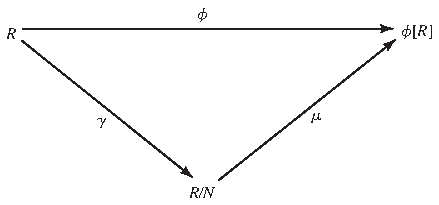
\includegraphics[width=0.602\linewidth,height=.8\textheight,keepaspectratio]{assets/p264_16.pdf}\end{center}
\begin{center}\small\textbf{30.18 Figure}\end{center}
\end{BookFloat}

\end{BookBody}

% Source PDF page 265; original printed page 248
\BookSource{265}{248}
\BookNarrativetrue

\begin{BookBody}

\BookLabel{\textit{Proof}} This follows at once from Theorems 30.15 and 30.16. Figure 30.18 is the analogue of Fig\BookInline{.12.15.}\BookEnd{\blacklozenge}

\BookLabel{30.19 Example} Example 30.3 shows that \BookInline{n\mathbb{Z}} is an ideal of \BookInline{\mathbb{Z},\allowbreak } so we can form the factor ring \BookInline{\mathbb{Z}/n\mathbb{Z}.} Example 22.11 shows that \BookInline{\phi:\mathbb{Z}\to \mathbb{Z}_{n}} where \BookInline{\phi (m)} is the remainder of \BookInline{m} modulo \BookInline{n} is a homomorphism, and we see that Ker\BookInline{(\phi )= n\mathbb{Z}.} Theorem 30.17 then shows that the map \BookInline{\mu:\mathbb{Z}/n\mathbb{Z}\to \mathbb{Z}_{n}} where \BookInline{\mu (m+ n\mathbb{Z})} is the remainder of \BookInline{m} modulo \BookInline{n} is well defined and is an isomorphism\BookInline{.}\BookEnd{\blacktriangle}

\BookLabel{30.20 Example} Continuing Example 30.5, let \BookInline{F} be the ring of all functions mapping \BookInline{\mathbb{R}} into \BookInline{\mathbb{R}} and let \BookInline{N} be the subset of \BookInline{F} consisting of all functions \BookInline{f} with \BookInline{f(2)= 0.} The set \BookInline{N} is an ideal in \BookInline{F,\allowbreak } so \BookInline{F/N} is a ring. Furthermore\BookInline{,\allowbreak N} is the kernel of the evaluation homomorphism \BookInline{\phi _{2}:F\to \mathbb{R}} defined by \BookInline{\phi _{2}(f)= f(2).} Since \BookInline{\phi _{2}} maps onto \BookInline{\mathbb{R},\allowbreak F/N} is isomorphic with \BookInline{\mathbb{R}} by Theorem 30.17. The function \BookInline{\mu:F/N\to \mathbb{R}} given by \BookInline{\mu (f)= f(2)} is an isomorphism. \BookEnd{\blacktriangle}

In summary, every ring homomorphism with domain \BookInline{R} gives rise to a factor ring \BookInline{R/N,\allowbreak } and every factor ring \BookInline{R/N} gives rise to a homomorphism mapping \BookInline{R} into \BookInline{R/N.} An \textit{ideal} in ring theory is analogous to a\textit{ normal subgroup} in the group theory. Both are the type of substructure needed to form a factor structure.

\end{BookBody}

\BookNarrativefalse

\begin{BookBody}

\BookExerciseTitle{30}

\BookTextHeading{\textbf{Computations}}

\BookExercise{1.}{Describe all ring homomorphisms of \BookInline{\mathbb{Z}\times \mathbb{Z}} into \BookInline{\mathbb{Z}\times \mathbb{Z}.[}\textit{Hint:} Note that if \BookInline{\phi } is such a homomorphism, then \BookInline{\phi ((1,\allowbreak 0))= \phi ((1,\allowbreak 0))\phi ((1,\allowbreak 0))} and \BookInline{\phi ((0,\allowbreak 1))= \phi ((0,\allowbreak 1))\phi ((0,\allowbreak 1)).} Consider also \BookInline{\phi ((1,\allowbreak 0)(0,\allowbreak 1)).]}}

\BookExercise{2.}{Find all positive integers \BookInline{n} such that \BookInline{\mathbb{Z}_{n}} contains a subring isomorphic to \BookInline{\mathbb{Z}_{2}.}}

\BookExercise{3.}{Find all ideals \BookInline{N} of \BookInline{\mathbb{Z}_{12}.} In each case compute \BookInline{\mathbb{Z}_{12}/N;} that is, find a known ring to which the quotient ring is isomorphic.}

\BookExercise{4.}{Give addition and multiplication tables for \BookInline{2\mathbb{Z}/8\mathbb{Z}.} Are \BookInline{2\mathbb{Z}/8\mathbb{Z}} and \BookInline{\mathbb{Z}_{4}} isomorphic rings?}

\BookTextHeading{\textbf{Concepts}}

\noindent In Exercises 5 through 7, correct the definition of the italicized term without reference to the text, if correction is needed, so that it is in a form acceptable for publication.

\BookExercise{5.}{An\textit{ isomorphism of} \BookInline{a} \textit{ring} \BookInline{R} with a ring \BookInline{R^{\prime }} is a homomorphism \BookInline{\phi:R\to R^{\prime }} such that Ker\BookInline{(\phi )= \{0\}.}}

\BookExercise{6.}{An\textit{ ideal} \BookInline{N} of a ring \BookInline{R} is an additive subgroup of \BookInline{\langle R,\allowbreak + \rangle } such that for all \BookInline{r\in R} and all \BookInline{n\in N,\allowbreak } we have \BookInline{rn\in N} and \BookInline{nr\in N.}}

\BookExercise{7.}{The\textit{ kernel of} \BookInline{a} \textit{homomorphism} \BookInline{\phi } mapping a ring \BookInline{R} into a ring \BookInline{R^{\prime }} is \BookInline{\{\phi (r)= 0^{\prime }\mid r\in R\}.}}

\BookExercise{8.}{Let \BookInline{F} be the ring of all functions mapping \BookInline{\mathbb{R}} into \BookInline{\mathbb{R}} and having derivatives of all orders. Differentiation gives a map \BookInline{\delta:F\to F} where \BookInline{\delta (f(x))= f^{\prime }(x).} Is \BookInline{\delta } a homomorphism? Why? Give the connection between this exercise and Example 30.4.}

\BookExercise{9.}{Give an example of a ring homomorphism \BookInline{\phi:R\to R^{\prime }} where \BookInline{R} has unity 1 and \BookInline{\phi (1)\neq 0^{\prime },\allowbreak } but \BookInline{\phi (1)} is not unity for \BookInline{R^{\prime }.}}

\BookExercise{10.}{Determine whether each of the following is true or false.}

\BookExercise{a.}{The concept of a ring homomorphism is closely connected with the idea of a factor ring.}

\BookExercise{b.}{A ring homomorphism \BookInline{\phi:R\to R^{\prime }} carries ideals of \BookInline{R} into ideals of \BookInline{R^{\prime }.}}

\BookExercise{c.}{A ring homomorphism is one-to-one if and only if the kernel is \BookInline{\{0\}.}}

\BookExercise{d.}{\textbf{d}\BookInline{.\mathbb{Q}} is an ideal in \BookInline{\mathbb{R}.}}

\end{BookBody}

% Source PDF page 266; original printed page 249
\BookSource{266}{249}
\BookNarrativefalse

\begin{BookBody}

\BookExercise{e.}{Every ideal in a ring is a subring of the ring.}

\BookExercise{f.}{Every subring of every ring is an ideal of the ring.}

\BookExercise{g.}{Every quotient ring of every commutative ring is again a commutative ring.}

\BookExercise{h.}{The rings \BookInline{\mathbb{Z}/4\mathbb{Z}} and \BookInline{\mathbb{Z}_{4}} are isomorphic.}

\BookExercise{i.}{An ideal \BookInline{N} in a ring \BookInline{R} with unity 1 is all of \BookInline{R} if and only if \BookInline{1\in N.}}

\BookExercise{j.}{The concept of an ideal is to the concept of a ring as the concept of a normal subgroup is to the concept of a group.}

\BookExercise{11.}{Let \BookInline{R} be a ring. Observe that \BookInline{\{0\}} and \BookInline{R} are both ideals of \BookInline{R.} Are the factor rings \BookInline{R/R} and \BookInline{R/\{0\}} of real interest? Why?}

\BookExercise{12.}{Give an example to show that a factor ring of an integral domain may be a field.}

\BookExercise{13.}{Give an example to show that a factor ring of an integral domain may have divisors of 0.}

\BookExercise{14.}{Give an example to show that a factor ring of a ring with divisors of 0 may be an integral domain.}

\BookExercise{15.}{Find a subring of the ring \BookInline{\mathbb{Z}\times \mathbb{Z}} that is not an ideal of \BookInline{\mathbb{Z}\times \mathbb{Z}.}}

\BookExercise{16.}{A student is asked to prove that a quotient ring of a ring \BookInline{R} modulo an ideal \BookInline{N} is commutative if and only if \BookInline{(rs- sr)\in N} for all \BookInline{r,\allowbreak s\in R.} The student starts out:}

Assume \BookInline{R/N} is commutative. Then \BookInline{rs= sr} for all \BookInline{r,\allowbreak s\in R/N.}

\BookExercise{a.}{Why does the instructor reading this expect an incorrect proof?}

\BookExercise{b.}{What should the student have written?}

\BookExercise{c.}{Prove the assertion. (Note the “if and only if.”)}

\BookTextHeading{\textbf{Theory}}

\BookInline{\Big[\Big]}

\BookExercise{17.}{Let \BookInline{R= \{a+ b\sqrt{2}\mid a,\allowbreak b\in \mathbb{Z}\}} and let \BookInline{R^{\prime }} consist of all \BookInline{2\times 2} matrices of the form \BookInline{\begin{bmatrix} a & 2b \\ b & a \end{bmatrix}} for \BookInline{a,\allowbreak b\in \mathbb{Z}.} Show that \BookInline{R} is a subring of \BookInline{\mathbb{R}} and that \BookInline{R^{\prime }} is a subring of \BookInline{M_{2}(\mathbb{Z}).} Then show that \BookInline{\phi:R\to R^{\prime },\allowbreak } where \BookInline{\phi (a+ b\sqrt{2})= } \BookInline{\begin{bmatrix} a & 2b \\ b & a \end{bmatrix}} is an isomorphism.}

\BookExercise{18.}{Show that each homomorphism from a field to a ring is either one-to-one or maps everything onto 0.}

\BookExercise{19.}{Show that if \BookInline{R,\allowbreak R^{\prime },\allowbreak } and \BookInline{R^{\prime \prime }} are rings, and if \BookInline{\phi:R\to R^{\prime }} and \BookInline{\psi:R^{\prime }\to R^{\prime \prime }} are homomorphisms, then the composite function \BookInline{\psi \phi:R\to R^{\prime \prime }} is a homomorphism. (See Exercise 39 of Section 8.)}

\BookExercise{20.}{Let \BookInline{R} be a commutative ring with unity of prime characteristic \BookInline{p.} Show that the map \BookInline{\phi _{p}:R\to R} given by \BookInline{\phi _{p}(a)= a^{p}} is a homomorphism (the\textbf{ Frobenius homomorphism}).}

\BookExercise{21.}{Let \BookInline{R} and \BookInline{R^{\prime }} be rings and let \BookInline{\phi:R\to R^{\prime }} be a ring homomorphism such that \BookInline{\phi [R]\neq \{0^{\prime }\}.} Show that if \BookInline{R} has unity 1 and \BookInline{R^{\prime }} has no 0 divisors, then \BookInline{\phi (1)} is unity for \BookInline{R^{\prime }.}}

\BookExercise{22.}{Let \BookInline{\phi:R\to R^{\prime }} be a ring homomorphism and let \BookInline{N} be an ideal of \BookInline{R.}}

\BookExercise{a.}{Show that \BookInline{\phi [N]} is an ideal of \BookInline{\phi [R].}}

\BookExercise{b.}{Give an example to show that \BookInline{\phi [N]} need not be an ideal of \BookInline{R^{\prime }.}}

\BookExercise{c.}{Let \BookInline{N^{\prime }} be an ideal either of \BookInline{\phi [R]} or of \BookInline{R^{\prime }.} Show that \BookInline{\phi ^{- 1}[N^{\prime }]} is an ideal of \BookInline{R.}}

\BookExercise{23.}{Let \BookInline{F} be a field, and let \BookInline{S} be any subset of \BookInline{F\times F\times \cdots \times F} for \BookInline{n} factors. Show that the set \BookInline{N_{S}} of all \BookInline{f(x_{1},\allowbreak \cdots,\allowbreak x_{n})\in F[x_{1},\allowbreak \cdots,\allowbreak x_{n}]} that have every element \BookInline{(a_{1},\allowbreak \cdots,\allowbreak a_{n})} of \BookInline{S} as a zero (see Exercise 28 of Section 27) is an ideal in \BookInline{F[x_{1},\allowbreak \cdots,\allowbreak x_{n}].} This is of importance in algebraic geometry.}

\BookExercise{24.}{Show that a factor ring of a field is either the trivial (zero) ring of one element or is isomorphic to the field.}

\BookExercise{25.}{Show that if \BookInline{R} is a ring with unity and \BookInline{N} is an ideal of \BookInline{R} such that \BookInline{N\neq R,\allowbreak } then \BookInline{R/N} is a ring with unity.}

\BookExercise{26.}{Let \BookInline{R} be a commutative ring and let \BookInline{a\in R.} Show that \BookInline{I_{a}= \{x\in R\mid } \textit{ax} \BookInline{= 0\}} is an ideal of \BookInline{R.}}

\BookExercise{27.}{Show that an intersection of ideals of a ring \BookInline{R} is again an ideal of \BookInline{R.}}

\BookExercise{28.}{Let \BookInline{R} and \BookInline{R^{\prime }} be rings and let \BookInline{N} and \BookInline{N^{\prime }} be ideals of \BookInline{R} and \BookInline{R^{\prime },\allowbreak } respectively. Let \BookInline{\phi } be a homomorphism of \BookInline{R} into \BookInline{R^{\prime }.} Show that \BookInline{\phi } induces a natural homomorphism \BookInline{\phi _{\ast }:R/N\to R^{\prime }/N^{\prime }} if \BookInline{\phi [N]\subseteq N^{\prime }.(}Use Exercise 41 of Section 12.)}

\end{BookBody}

% Continuation on source PDF page 267, preceding Section 31
\BookNarrativefalse

\begin{BookBody}

\BookExercise{29.}{Let \BookInline{\phi } be a homomorphism of a ring \BookInline{R} with unity onto a nonzero ring \BookInline{R^{\prime }.} Let \BookInline{u} be a unit in \BookInline{R.} Show that \BookInline{\phi (u)} is a unit in \BookInline{R^{\prime }.}}

\BookExercise{30.}{An element \BookInline{a} of a ring \BookInline{R} is\textbf{ nilpotent} if \BookInline{a^{n}= 0} for some \BookInline{n\in \mathbb{Z}^{+ }.} Show that the collection of all nilpotent elements in a commutative ring \BookInline{R} is an ideal, the\textbf{ nilradical of} \BookInline{R.}}

\BookExercise{31.}{Referring to the definition given in Exercise 30, find the nilradical of the ring \BookInline{\mathbb{Z}_{12}} and observe that it is one of the ideals of \BookInline{\mathbb{Z}_{12}} found in Exercise 3. What is the nilradical of \BookInline{\mathbb{Z}}? of \BookInline{\mathbb{Z}_{32}}?}

\BookExercise{32.}{Referring to Exercise 30, show that if \BookInline{N} is the nilradical of a commutative ring \BookInline{R,\allowbreak } then \BookInline{R/N} has as nilradical the trivial ideal \BookInline{\{0+ N\}.}}

\BookExercise{33.}{Let \BookInline{R} be a commutative ring and \BookInline{N} an ideal of \BookInline{R.} Referring to Exercise 30, show that if every element of \BookInline{N} is nilpotent and the nilradical of \BookInline{R/N} is \BookInline{R/N,\allowbreak } then the nilradical of \BookInline{R} is \BookInline{R.}}

\BookExercise{34.}{Let \BookInline{R} be a commutative ring and \BookInline{N} an ideal of \BookInline{R.} Show that the set \BookInline{\sqrt{N}} of all \BookInline{a\in R,\allowbreak } such that \BookInline{a^{n}\in N} for some \BookInline{n\in \mathbb{Z}^{+ },\allowbreak } is an ideal of \BookInline{R,\allowbreak } the\textbf{ radical of} \BookInline{N.}}

\BookExercise{35.}{Referring to Exercise 34, show by examples that for proper ideals \BookInline{N} of a commutative ring \BookInline{R,\allowbreak }}

\textbf{a}\BookInline{.\sqrt{N}} need not equal \BookInline{N} \textbf{b}\BookInline{.\sqrt{N}} may equal \BookInline{N.}

\BookExercise{36.}{What is the relationship of the ideal \BookInline{\sqrt{N}} of Exercise 34 to the nilradical of \BookInline{R/N(}see Exercise 30)? Word your answer carefully.}

\BookExercise{37.}{Show that \BookInline{\phi:\mathbb{C}\to M_{2}(\mathbb{R})} given by}

\begin{center}\begin{adjustbox}{max width=\linewidth}\BookInline{\displaystyle \phi(a + bi) = \begin{pmatrix} a & b \\ -b & a \end{pmatrix}}\end{adjustbox}\end{center}

for \BookInline{a,\allowbreak b\in \mathbb{R}} gives an isomorphism of \BookInline{\mathbb{C}} with the subring \BookInline{\phi [\mathbb{C}]} of \BookInline{M_{2}(\mathbb{R}).}

\end{BookBody}
\ifdefined\BookMaster\let\BookFinish\relax\else\def\BookFinish{\end{document}}\fi\BookFinish

\clearpage
% !TeX program = xelatex
\ifdefined\BookMaster\else
\documentclass[11pt,oneside]{article}
% !TeX program = xelatex
\usepackage[b5paper,left=22mm,right=22mm,top=20mm,bottom=22mm,footskip=11mm]{geometry}
\usepackage{fontspec}
\setmainfont{TeX Gyre Termes}
\setsansfont{TeX Gyre Heros}
\usepackage{amsmath,amssymb,mathtools,amsthm}
\renewcommand{\cdots}{\mathinner{\cdotp\cdotp\cdotp}}
\usepackage{graphicx,adjustbox,array,booktabs,longtable,multirow,enumitem,changepage,needspace}
\usepackage[table]{xcolor}
\usepackage{fancyhdr}
\raggedbottom
\interfootnotelinepenalty=10000
\newcommand{\BookFootnote}[2]{\begingroup\renewcommand{\thefootnote}{\fnsymbol{footnote}}\footnote[#1]{#2}\endgroup}
\newcommand{\BookFootnoteMark}[1]{\begingroup\renewcommand{\thefootnote}{\fnsymbol{footnote}}\footnotemark[#1]\endgroup}
\newcommand{\BookFootnoteText}[2]{\begingroup\renewcommand{\thefootnote}{\fnsymbol{footnote}}\footnotetext[#1]{#2}\endgroup}
\newenvironment{BookFloat}[1]{\par\addvspace{.6\baselineskip}\noindent\def\BookFloatID{#1}\begin{minipage}{\linewidth}\phantomsection\label{bookfloat:#1:start}}{\phantomsection\label{bookfloat:\BookFloatID:end}\end{minipage}\par\addvspace{.6\baselineskip}}

\usepackage[unicode,hidelinks]{hyperref}
\pagestyle{fancy}
\fancyhf{}
\newcommand{\BookFooter}{}
\fancyfoot[L]{\parbox[b]{\dimexpr\textwidth-15mm}{\footnotesize\BookFooter}}
\fancyfoot[R]{\footnotesize\thepage}
\renewcommand{\headrulewidth}{0pt}
\renewcommand{\footrulewidth}{0pt}
\setlength{\parindent}{0pt}
\setlength{\parskip}{0.2em}
\setlength{\emergencystretch}{3em}
\setlist{nosep,leftmargin=1.7em,labelsep=.65em}
\newif\ifBookNarrative
\BookNarrativetrue
\newenvironment{BookBody}{\setlength{\parindent}{0pt}}{}
\newcommand{\BookStatement}[1]{\par\addvspace{.6\baselineskip}\noindent #1\enspace\ignorespaces}
\newcommand{\BookLabel}[1]{\par\addvspace{.6\baselineskip}\needspace{3\baselineskip}\noindent\textbf{#1}\quad\ignorespaces}
\newcommand{\BookHeading}[1]{\par\addvspace{\baselineskip}\needspace{4\baselineskip}\noindent{\large\bfseries #1}\par\medskip}
\newcommand{\BookSubheading}[1]{\par\addvspace{.7\baselineskip}\needspace{3\baselineskip}\noindent{\bfseries #1}\par\smallskip}
\newcommand{\BookTextHeading}[1]{\par\addvspace{.7\baselineskip}\needspace{3\baselineskip}\noindent #1\par\smallskip}
\newcommand{\BookSectionTitle}[2]{\par\addvspace{1.2\baselineskip}\needspace{5\baselineskip}\noindent\colorbox{gray!25}{\sffamily\bfseries\small SECTION #1}\quad{\large\bfseries #2}\par\medskip}
\newcommand{\BookExerciseTitle}[1]{\par\addvspace{\baselineskip}\needspace{4\baselineskip}\noindent{\color{gray}\rule{1.5mm}{1.5mm}}\enspace{\large\bfseries Exercises #1}\par\medskip}
\newcommand{\BookBullet}[1]{\begin{list}{\textbullet}{\setlength{\leftmargin}{1.7em}\setlength{\labelwidth}{1em}\setlength{\labelsep}{.7em}\setlength{\topsep}{0pt}\setlength{\parsep}{0pt}\setlength{\itemsep}{0pt}}\item #1\end{list}}
\newcommand{\BookExercise}[2]{\begin{list}{\textbf{#1}}{\setlength{\leftmargin}{2.2em}\setlength{\labelwidth}{1.5em}\setlength{\labelsep}{.7em}\setlength{\topsep}{.15em}\setlength{\parsep}{0pt}\setlength{\itemsep}{0pt}}\item #2\end{list}}
\newcommand{\BookEnd}[1]{\unskip\nobreak\hfill\ensuremath{#1}}
\newcommand{\BookSource}[2]{\phantomsection\label{sourcepage:#1}} % Source-page anchors, retained through reflow.
\usepackage{multicol}
\usepackage{tikz}
\newcommand{\BookPartEntry}[2]{\par\noindent\makebox[17mm][l]{\bfseries Section #1}#2\par}
\newcommand{\BookPartTitle}[3]{\par\bigskip\noindent\begin{tikzpicture}\node[anchor=north west,inner sep=0pt,outer sep=0pt] (bookpart) at (0,0) {\begin{minipage}{\dimexpr\linewidth-.5pt}\hspace*{26mm}\begin{minipage}[t]{\dimexpr\linewidth-26mm}\begin{adjustbox}{max width=\linewidth}{\fontsize{20}{24}\selectfont\bfseries #2}\end{adjustbox}\par\vspace{6mm}\hrule\vspace{6mm}{\sffamily\footnotesize\setlength{\parskip}{.3em}#3}\vspace{3mm}\end{minipage}\end{minipage}};\path[shade,top color=gray!60,bottom color=white] (0,0) rectangle ([xshift=24mm]bookpart.south west);\node[anchor=north,font=\sffamily\bfseries\small] at (12mm,-2mm) {PART};\node[anchor=north,font=\sffamily\bfseries\Huge] at (12mm,-7mm) {#1};\end{tikzpicture}\par\bigskip}
\newsavebox{\BookMathBox}
\makeatletter
\newcommand{\BookInline}[1]{\leavevmode\hskip0pt\relax\begingroup\in@{\begin}{#1}\ifin@\sbox{\BookMathBox}{\(#1\)}\ifdim\wd\BookMathBox>\dimexpr\linewidth-1em\relax\resizebox{\dimexpr\linewidth-1em\relax}{!}{\usebox{\BookMathBox}}\else\(#1\)\fi\else\in@{\left}{#1}\ifin@\sbox{\BookMathBox}{\(#1\)}\ifdim\wd\BookMathBox>\dimexpr\linewidth-1em\relax\resizebox{\dimexpr\linewidth-1em\relax}{!}{\usebox{\BookMathBox}}\else\(#1\)\fi\else\(#1\)\fi\fi\endgroup\hskip0pt\relax}
\makeatother
\DeclareMathOperator{\Aut}{Aut}
\DeclareMathOperator{\End}{End}
\DeclareMathOperator{\Hom}{Hom}
\DeclareMathOperator{\GF}{GF}
\DeclareMathOperator{\irr}{irr}
\DeclareMathOperator{\lt}{lt}
\DeclareMathOperator{\lp}{lp}
\providecommand{\textcircled}[1]{\textnormal{(#1)}}

\begin{document}
\fi
\renewcommand{\BookFooter}{Section 31 Prime and Maximal Ideals}
\pdfbookmark[0]{Section 31 Prime and Maximal Ideals}{31_prime_and_maximal_ideals}
\ifdefined\BookMaster\else\setcounter{page}{250}\fi
% Source PDF page 267; original printed page 250
\BookSource{267}{250}
\BookNarrativetrue

\begin{BookBody}

\BookSectionTitle{31}{Prime and Maximal Ideals}

\noindent Exercises 12 through 14 of the preceding section asked us to provide examples of factor rings \BookInline{R/N} where \BookInline{R} and \BookInline{R/N} have very different structural properties. We start with some examples of this situation, and in the process, provide solutions to those exercises.

\BookLabel{31.1 Example} As was shown in Corollary 23.5, the ring \BookInline{\mathbb{Z}_{p},\allowbreak } which is isomorphic to \BookInline{\mathbb{Z}/p\mathbb{Z},\allowbreak } is a field for \BookInline{p} a prime.\textit{ Thus} \BookInline{a} \textit{factor ring of an integral domain may be} \BookInline{a\text{fi}eld.}\BookEnd{\blacktriangle}

\BookLabel{31.2 Example} The ring \BookInline{\mathbb{Z}\times \mathbb{Z}} is not an integral domain, for

\begin{center}\begin{adjustbox}{max width=\linewidth}\BookInline{\displaystyle (0,\allowbreak 1)(1,\allowbreak 0)= (0,\allowbreak 0),\allowbreak }\end{adjustbox}\end{center}

\noindent showing that (0, 1) and (1, 0) are 0 divisors. Let \BookInline{N= \{(0,\allowbreak n)\mid n\in \mathbb{Z}\}.} Now \BookInline{N} is an ideal of \BookInline{\mathbb{Z}\times \mathbb{Z},\allowbreak } and \BookInline{(\mathbb{Z}\times \mathbb{Z})/N} is isomorphic to \BookInline{\mathbb{Z}} under the correspondence \BookInline{[(m,\allowbreak 0)+ N]\leftrightarrow } \BookInline{m,\allowbreak } where \BookInline{m\in \mathbb{Z}.} Thus a\textit{ factor} ring of a ring may be an integral domain, even though the original ring is not\BookInline{.}\BookEnd{\blacktriangle}

\BookLabel{31.3 Example} The subset \BookInline{N= \{0,\allowbreak 3\}} of \BookInline{\mathbb{Z}_{6}} is easily seen to be an ideal of \BookInline{\mathbb{Z}_{6},\allowbreak } and \BookInline{\mathbb{Z}_{6}/N} has three elements\BookInline{,\allowbreak 0+ N,\allowbreak 1+ N,\allowbreak } and \BookInline{2+ N.} These add and multiply in such a fashion as to show that \BookInline{\mathbb{Z}_{6}/N\simeq \mathbb{Z}_{3}} under the correspondence

\begin{center}\begin{adjustbox}{max width=\linewidth}\BookInline{\displaystyle (0+ N)\leftrightarrow 0,\allowbreak (1+ N)\leftrightarrow 1,\allowbreak (2+ N)\leftrightarrow 2.}\end{adjustbox}\end{center}

\noindent This example shows that\textit{ if} \BookInline{R} \textit{is not even an integral domain, that is, if} \BookInline{R} \textit{has zero} \textit{divisors, it is still possible for} \BookInline{R/N} \textit{to be} \BookInline{a\text{fi}eld.}\BookEnd{\blacktriangle}

\BookLabel{31.4 Example} Note that \BookInline{\mathbb{Z}} is an integral domain, but \BookInline{\mathbb{Z}/6\mathbb{Z}\simeq \mathbb{Z}_{6}} is not. The preceding examples showed that a factor ring may have a structure that seems\textit{ better} than the original ring.

\end{BookBody}

% Source PDF page 268; original printed page 251
\BookSource{268}{251}
\BookNarrativetrue

\begin{BookBody}

\noindent This example indicates that the structure of a factor ring may seem\textit{ worse} than that of the original ring\BookInline{.}\BookEnd{\blacktriangle}

Every nonzero ring \BookInline{R} has at least two ideals, the\textbf{ improper ideal} \BookInline{R} and the\textbf{ trivial} \textbf{ideal} \BookInline{\{0\}.} For these ideals, the factor rings are \BookInline{R/R,\allowbreak } which has only one element, and \BookInline{R/\{0\},\allowbreak } which is isomorphic to \BookInline{R.} These are uninteresting cases. Just as for a subgroup of a group, a\textbf{ proper nontrivial ideal} of a ring \BookInline{R} is an ideal \BookInline{N} of \BookInline{R} such that \BookInline{N\neq R} and \BookInline{N\neq \{0\}.}

While factor rings of rings and integral domains may be of great interest, as the above examples indicate, Corollary 31.6, which follows our next theorem, shows that a factor ring of a field is really not useful to us.

\BookLabel{31.5 Theorem} If \BookInline{R} is a ring with unity, and \BookInline{N} is an ideal of \BookInline{R} containing a unit, then \BookInline{N= R.}

\BookLabel{\textit{Proof}} Let \BookInline{N} be an ideal of \BookInline{R,\allowbreak } and suppose that \BookInline{u\in N} for some unit \BookInline{u} in \BookInline{R.} Then the condition \BookInline{rN\subseteq N} for all \BookInline{r\in R} implies, if we take \BookInline{r= u^{- 1}} and \BookInline{u\in N,\allowbreak } that \BookInline{1= u^{- 1}u} is in \BookInline{N.} But then \BookInline{rN\subseteq N} for all \BookInline{r\in R} implies that \BookInline{r1= r} is in \BookInline{N} for all \BookInline{r\in R,\allowbreak } so \BookInline{N= R.}\BookEnd{\blacklozenge}

\BookLabel{31.6 Corollary} A field contains no proper nontrivial ideals.

\BookLabel{\textit{Proof}} Since every nonzero element of a field is a unit, it follows at once from Theorem 31.5 that an ideal of a field \BookInline{F} is either \BookInline{\{0\}} or all of \BookInline{F.}\BookEnd{\blacklozenge}

\BookTextHeading{\textbf{Maximal and Prime Ideals}  }

\noindent We now consider the questions of when a factor ring is a field and when it is an integral domain. In our analogy between groups and rings, we noticed that ideals in rings correspond to normal subgroups. Corollary 31.6 states that a field contains no proper nontrivial ideals. In group theory, this corresponds to a group having no proper nontrivial normal subgroups, that is, a simple group. Theorem 13.20 states that a factor group \BookInline{G/H} is simple if and only if \BookInline{H} is a maximal normal subgroup of \BookInline{G.} The following definition is analogous to maximal normal subgroups.

\BookLabel{31.7 Definition} A\textbf{ maximal ideal of a ring} \BookInline{R} is an ideal \BookInline{M} different from \BookInline{R} such that there is no proper ideal \BookInline{N} of \BookInline{R} properly containing \BookInline{M.}\BookEnd{\blacksquare}

\BookLabel{31.8 Example} Let \BookInline{p} be a prime positive integer. We know that \BookInline{\mathbb{Z}/p\mathbb{Z}} is isomorphic to \BookInline{\mathbb{Z}_{p}.} Forgetting about multiplication for the moment and regarding \BookInline{\mathbb{Z}/p\mathbb{Z}} and \BookInline{\mathbb{Z}_{p}} as additive groups, we know that \BookInline{\mathbb{Z}_{p}} is a simple group, and consequently \BookInline{p\mathbb{Z}} must be a maximal normal subgroup of \BookInline{\mathbb{Z}} by Theorem 13.20. Since \BookInline{\mathbb{Z}} is an abelian group and every subgroup is a normal subgroup, we see that \BookInline{p\mathbb{Z}} is a maximal proper subgroup of \BookInline{\mathbb{Z}.} Since \BookInline{p\mathbb{Z}} is an ideal of the ring \BookInline{\mathbb{Z},\allowbreak } it follows that \BookInline{p\mathbb{Z}} is a maximal ideal of \BookInline{\mathbb{Z}.} We know that \BookInline{\mathbb{Z}/p\mathbb{Z}} is isomorphic to the ring \BookInline{\mathbb{Z}_{p},\allowbreak } and that \BookInline{\mathbb{Z}_{p}} is actually a field. Thus \BookInline{\mathbb{Z}/p\mathbb{Z}} is a field. This illustrates the next theorem\BookInline{.}\BookEnd{\blacktriangle}

\BookLabel{31.9 Theorem} \textbf{(Analogue of Theorem 13.20)} Let \BookInline{R} be a commutative ring with unity. Then \BookInline{M} is a maximal ideal of \BookInline{R} if and only if \BookInline{R/M} is a field.

\BookLabel{\textit{Proof}} We first assume that \BookInline{M} is a maximal ideal in \BookInline{R.} Since \BookInline{R} is a commutative ring with unity, so is \BookInline{R/M.} Furthermore, since \BookInline{M\neq R,\allowbreak 0+ M\neq 1+ M} and \BookInline{R/M} is a nonzero ring. Let \BookInline{(a+ M)\in R/M,\allowbreak } with \BookInline{a\notin M,\allowbreak } so that \BookInline{a+ M} is not the additive identity element of \BookInline{R/M.} Suppose \BookInline{a+ M} has no multiplicative inverse in \BookInline{R/M.} Then the set \BookInline{(R/M)(a+ M)= \{(r+ M)(a+ M)\mid (r+ M)\in R/M\}} does not contain \BookInline{1+ M.} We easily see that \BookInline{(R/M)(a+ M)} is an ideal of \BookInline{R/M.} It is nontrivial because \BookInline{a\notin M,\allowbreak } and it is a 
% Source PDF page 269; original printed page 252
\BookSource{269}{252}
proper ideal because it does not contain \BookInline{1+ M.} By Theorem 30.11, if \BookInline{\gamma:R\to R/M} is the canonical homomorphism, then \BookInline{\gamma ^{- 1}[(R/M)(a+ M)]} is a proper ideal of \BookInline{R} properly containing \BookInline{M.} But this contradicts our assumption that \BookInline{M} is a maximal ideal, so \BookInline{a+ M} must have a multiplicative inverse in \BookInline{R/M.}

\end{BookBody}

\BookNarrativetrue

\begin{BookBody}

Conversely, suppose that \BookInline{R/M} is a field. By Theorem 30.11, if \BookInline{N} is any ideal of \BookInline{R} such that \BookInline{M\subset N\subset R} and \BookInline{\gamma } is the canonical homomorphism of \BookInline{R} onto \BookInline{R/M,\allowbreak } then \BookInline{\gamma [N]} is an ideal of \BookInline{R/M} with \BookInline{\{(0+ M)\}\subset \gamma [N]\subset R/M.} But this is contrary to Corollary 31.6, which states that the field \BookInline{R/M} contains no proper nontrivial ideals. Hence if \BookInline{R/M} is a field, then \BookInline{M} is maximal\BookInline{.}\BookEnd{\blacklozenge}

\BookLabel{31.10 Example} Since \BookInline{\mathbb{Z}/n\mathbb{Z}} is isomorphic to \BookInline{\mathbb{Z}_{n}} and \BookInline{\mathbb{Z}_{n}} is a field if and only if \BookInline{n} is a prime, we see that the maximal ideals of \BookInline{\mathbb{Z}} are precisely the ideals \BookInline{p\mathbb{Z}} for prime positive integers \BookInline{p.}\BookEnd{\blacktriangle}

\BookLabel{31.11 Corollary} A commutative ring with unity is a field if and only if it has no proper nontrivial ideals.

\BookLabel{\textit{Proof}} Corollary 31.6 shows that a field has no proper nontrivial ideals.

Conversely, if a commutative ring \BookInline{R} with unity has no proper nontrivial ideals, then \BookInline{\{0\}} is a maximal ideal and \BookInline{R/\{0\},\allowbreak } which is isomorphic to \BookInline{R,\allowbreak } is a field by Theorem 31.9. \BookEnd{\blacklozenge}

We now turn to the question of characterizing, for a commutative ring \BookInline{R} with unity, the ideals \BookInline{N\neq R} such that \BookInline{R/N} is an integral domain. The answer here is rather obvious. The factor ring \BookInline{R/N} will be an integral domain if and only if \BookInline{(a+ N)(b+ N)= N} implies that either

\begin{center}\begin{adjustbox}{max width=\linewidth}\BookInline{\displaystyle a+ N= N\;\text{or}\;b+ N= N.}\end{adjustbox}\end{center}

\noindent This is exactly the statement that \BookInline{R/N} has no divisors of 0, since the coset \BookInline{N} plays the role of 0 in \BookInline{R/N.} Looking at representatives, we see that this condition amounts to saying that \BookInline{ab\in N} implies that either \BookInline{a\in N} or \BookInline{b\in N.}

\BookLabel{31.12 Example} All ideals of \BookInline{\mathbb{Z}} are of the form \BookInline{n\mathbb{Z}.} For \BookInline{n= 0,\allowbreak } we have \BookInline{n\mathbb{Z}= \{0\},\allowbreak } and \BookInline{\mathbb{Z}/\{0\}\simeq \mathbb{Z},\allowbreak } which is an integral domain. For \BookInline{n>0,\allowbreak } we have \BookInline{\mathbb{Z}/n\mathbb{Z}\simeq \mathbb{Z}_{n}} and \BookInline{\mathbb{Z}_{n}} is an integral domain if and only if \BookInline{n} is a prime. Thus the nonzero ideals \BookInline{n\mathbb{Z}} such that \BookInline{\mathbb{Z}/n\mathbb{Z}} is an integral domain are of the form \BookInline{p\mathbb{Z},\allowbreak } where \BookInline{p} is a prime. Of course\BookInline{,\allowbreak \mathbb{Z}/p\mathbb{Z}} is actually a field, so that \BookInline{p\mathbb{Z}} is a maximal ideal of \BookInline{\mathbb{Z}.} Note that for a product \BookInline{rs} of integers to be in \BookInline{p\mathbb{Z},\allowbreak } the prime \BookInline{p} must divide either \BookInline{r} or \BookInline{s.} The role of prime integers in this example makes the use of the word\textit{ prime} in the next definition more reasonable\BookInline{.}\BookEnd{\blacktriangle}

\BookLabel{31.13 Definition} An ideal \BookInline{N\neq R} in a commutative ring \BookInline{R} is a\textbf{ prime ideal} if \BookInline{ab\in N} implies that either \BookInline{a\in N} or \BookInline{b\in N} for \BookInline{a,\allowbreak b\in R.}\BookEnd{\blacksquare}

Note that \BookInline{\{0\}} is a prime ideal in \BookInline{\mathbb{Z},\allowbreak } and indeed, in any integral domain.

\BookLabel{31.14 Example} Note that \BookInline{\mathbb{Z}\times \{0\}} is a prime ideal of \BookInline{\mathbb{Z}\times \mathbb{Z},\allowbreak } for if \BookInline{(a,\allowbreak b)(c,\allowbreak d)\in \mathbb{Z}\times \{0\},\allowbreak } then we must have \BookInline{bd= 0} in \BookInline{\mathbb{Z}.} This implies that either \BookInline{b= 0} so \BookInline{(a,\allowbreak b)\in \mathbb{Z}\times \{0\}} or \BookInline{d= 0} so \BookInline{(c,\allowbreak d)\in } \BookInline{\mathbb{Z}\times \{0\}.} Note that \BookInline{(\mathbb{Z}\times \mathbb{Z})/(\mathbb{Z}\times \{0\})} is isomorphic to \BookInline{\mathbb{Z},\allowbreak } which is an integral domain. \BookEnd{\blacktriangle}

Our remarks preceding Example 31.12 constitute a proof of the following theorem, which is illustrated by Example 31.14.

\BookLabel{31.15 Theorem} Let \BookInline{R} be a commutative ring with unity, and let \BookInline{N\neq R} be an ideal in \BookInline{R.} Then \BookInline{R/N} is an integral domain if and only if \BookInline{N} is a prime ideal in \BookInline{R.}

\end{BookBody}

% Source PDF page 270; original printed page 253
\BookSource{270}{253}
\BookNarrativetrue

\begin{BookBody}

\BookLabel{31.16 Corollary} Every maximal ideal in a commutative ring \BookInline{R} with unity is a prime ideal.

\BookLabel{\textit{Proof}} If \BookInline{M} is maximal in \BookInline{R,\allowbreak } then \BookInline{R/M} is a field, hence an integral domain, and therefore \BookInline{M} is a prime ideal by Theorem \BookInline{31.15.}\BookEnd{\blacklozenge}

The material that has just been presented regarding maximal and prime ideals is very important and we shall be using it quite a lot. We should keep the main ideas well in mind. We must know and understand the definitions of maximal and prime ideals and must remember the following facts that we have demonstrated.

For a commutative ring \BookInline{R} with unity:

\BookExercise{1.}{An ideal \BookInline{M} of \BookInline{R} is maximal if and only if \BookInline{R/M} is a field.}

\BookExercise{2.}{An ideal \BookInline{N} of \BookInline{R} is prime if and only if \BookInline{R/N} is an integral domain.}

\BookExercise{3.}{Every maximal ideal of \BookInline{R} is a prime ideal.}

\BookTextHeading{\textbf{Prime Fields}  }

\noindent We now proceed to show that the rings \BookInline{\mathbb{Z}} and \BookInline{\mathbb{Z}_{n}} form foundations upon which all rings with unity rest, and that \BookInline{\mathbb{Q}} and \BookInline{\mathbb{Z}_{p}} perform a similar service for all fields. Let \BookInline{R} be any ring with unity 1. Recall that by \BookInline{n\cdot 1} we mean \BookInline{1+ 1+ \cdots + 1} for \BookInline{n} summands for \BookInline{n>0,\allowbreak } and \BookInline{(- 1)+ (- 1)+ \cdots + (- 1)} for \BookInline{|n|} summands for \BookInline{n<0,\allowbreak } while \BookInline{n\cdot 1= 0} for \BookInline{n= 0.}

\BookLabel{31.17 Theorem} If \BookInline{R} is a ring with unity 1, then the map \BookInline{\phi:\mathbb{Z}\to R} given by

\begin{center}\begin{adjustbox}{max width=\linewidth}\BookInline{\displaystyle \phi (n)= n\cdot 1}\end{adjustbox}\end{center}

\noindent for \BookInline{n\in \mathbb{Z}} is a homomorphism of \BookInline{\mathbb{Z}} into \BookInline{R.}

\BookLabel{\textit{Proof}} Observe that

\begin{center}\begin{adjustbox}{max width=\linewidth}\BookInline{\displaystyle \phi (n+ m)= (n+ m)\cdot 1= (n\cdot 1)+ (m\cdot 1)= \phi (n)+ \phi (m).}\end{adjustbox}\end{center}

\noindent The distributive laws in \BookInline{R} show that

\begin{center}\begin{adjustbox}{max width=\linewidth}\BookInline{\displaystyle \underbrace { ( 1 + 1 + \cdots + 1 ) } _ { n \mathrm { \scriptsize ~ s u m m a n d s } } \underbrace { ( 1 + 1 + \cdots + 1 ) } _ { m \mathrm { \scriptsize ~ s u m m a n d s } } = \underbrace { ( 1 + 1 + \cdots + 1 ) } _ { n m \mathrm { \scriptsize ~ s u m m a n d s } } .}\end{adjustbox}\end{center}

Thus \BookInline{(n\cdot 1)(m\cdot 1)= (nm)\cdot 1} for \BookInline{n,\allowbreak m>0.} Similar arguments with the distributive laws show that for all \BookInline{n,\allowbreak m\in \mathbb{Z},\allowbreak } we have

\begin{center}\begin{adjustbox}{max width=\linewidth}\BookInline{\displaystyle (n\cdot 1)(m\cdot 1)= (nm)\cdot 1.}\end{adjustbox}\end{center}

\noindent Thus

\begin{center}\begin{adjustbox}{max width=\linewidth}\BookInline{\displaystyle \phi (nm)= (nm)\cdot 1= (n\cdot 1)(m\cdot 1)= \phi (n)\phi (m).}\end{adjustbox}\end{center} \BookEnd{\blacklozenge}

\BookLabel{31.18 Corollary} Let \BookInline{R} be a ring with unity. If \BookInline{R} has characteristic \BookInline{n>1,\allowbreak } then \BookInline{R} contains a subring isomorphic to \BookInline{\mathbb{Z}_{n}.} If \BookInline{R} has characteristic 0, then \BookInline{R} contains a subring isomorphic to \BookInline{\mathbb{Z}.}

\BookLabel{\textit{Proof}} The map \BookInline{\phi:\mathbb{Z}\to R} given by \BookInline{\phi (m)= m\cdot 1} for \BookInline{m\in \mathbb{Z}} is a homomorphism by Theorem 31.17. The kernel must be an ideal in \BookInline{\mathbb{Z}.} All ideals in \BookInline{\mathbb{Z}} are of the form \BookInline{s\mathbb{Z}} for some \BookInline{s\in \mathbb{Z}.} By Theorem 23.14 we see that if \BookInline{R} has characteristic \BookInline{n>0,\allowbreak } then the kernel of \BookInline{\phi } is \BookInline{n\mathbb{Z}.} Then the image \BookInline{\phi [\mathbb{Z}]\leq R} is isomorphic to \BookInline{\mathbb{Z}/n\mathbb{Z}\simeq \mathbb{Z}_{n}.} If the characteristic of \BookInline{R} is 0, then \BookInline{m\cdot 1\neq 0} for all \BookInline{m\neq 0,\allowbreak } so the kernel of \BookInline{\phi } is \BookInline{\{0\}.} Thus, the image \BookInline{\phi [\mathbb{Z}]\leq R} is isomorphic to \BookInline{\mathbb{Z}.}\BookEnd{\blacklozenge}

\end{BookBody}

% Source PDF page 271; original printed page 254
\BookSource{271}{254}
\BookNarrativetrue

\begin{BookBody}

\BookLabel{31.19 Theorem} A field \BookInline{F} is either of prime characteristic \BookInline{p} and contains a subfield isomorphic to \BookInline{\mathbb{Z}_{p}} or of characteristic 0 and contains a subfield isomorphic to \BookInline{\mathbb{Q}.}

\BookLabel{\textit{Proof}} If the characteristic of \BookInline{F} is not 0, the above corollary shows that \BookInline{F} contains a subring isomorphic to \BookInline{\mathbb{Z}_{n}.} Then \BookInline{n} must be a prime \BookInline{p,\allowbreak } or \BookInline{F} would have 0 divisors. If \BookInline{F} is of characteristic 0, then \BookInline{F} must contain a subring isomorphic to \BookInline{\mathbb{Z}.} In this case Corollaries 26.9 and 26.10 show that \BookInline{F} must contain a field of quotients of this subring and that this field of quotients must be isomorphic to \BookInline{\mathbb{Q}.}\BookEnd{\blacklozenge}

Thus every field contains either a subfield isomorphic to \BookInline{\mathbb{Z}_{p}} for some prime \BookInline{p} or a subfield isomorphic to \BookInline{\mathbb{Q}.} These fields \BookInline{\mathbb{Z}_{p}} and \BookInline{\mathbb{Q}} are the fundamental building blocks on which all fields rest.

\BookLabel{31.20 Definition} The fields \BookInline{\mathbb{Z}_{p}} and \BookInline{\mathbb{Q}} are\textbf{ prime fields.} \BookEnd{\blacksquare}

\BookTextHeading{\textbf{Ideal Structure in} \textit{\textbf{F}}\textbf{[}\textit{\textbf{x}}\textbf{]}   }

\noindent Throughout the rest of this section, we assume that \BookInline{F} is a field. We give the next definition for a general commutative ring \BookInline{R} with unity, although we are only interested in the case \BookInline{R= F[x].} Note that for a commutative ring \BookInline{R} with unity and \BookInline{a\in R,\allowbreak } the set \BookInline{\{}\textit{ra} \BookInline{\mid r\in R\}} is an ideal in \BookInline{R} that contains the element \BookInline{a.}

\BookLabel{31.21 Definition} If \BookInline{R} is a commutative ring with unity and \BookInline{a\in R,\allowbreak } the ideal \BookInline{\{}\textit{ra} \BookInline{\mid r\in R\}} of all multiples of \BookInline{a} is the\textbf{ principal ideal generated by} \BookInline{a} and is denoted by \BookInline{\langle a\rangle.} An ideal \BookInline{N} of \BookInline{R} is a \textbf{principal ideal} if \BookInline{N= \langle a\rangle } for some \BookInline{a\in R.}\BookEnd{\blacksquare}

\BookLabel{31.22 Example} Every ideal of the ring \BookInline{\mathbb{Z}} is of the form \BookInline{n\mathbb{Z},\allowbreak } which is generated by \BookInline{n,\allowbreak } so every ideal of \BookInline{\mathbb{Z}} is a principal ideal\BookInline{.}\BookEnd{\blacktriangle}

\BookLabel{31.23 Example} The principal ideal \BookInline{\langle x\rangle } in \BookInline{F[x]} consists of all polynomials in \BookInline{F[x]} having zero constant term\BookInline{.}\BookEnd{\blacktriangle}

The next theorem is another simple but very important application of the division algorithm for \BookInline{F[x].(}See Theorem 28.2.) The proof of this theorem is to the division algorithm in \BookInline{F[x]} as the proof that a subgroup of a cyclic group is cyclic is to the division algorithm in \BookInline{\mathbb{Z}.}

\BookLabel{31.24 Theorem} If \BookInline{F} is a field, every ideal in \BookInline{F[x]} is principal.

\BookLabel{\textit{Proof}} Let \BookInline{N} be an ideal of \BookInline{F[x].} If \BookInline{N= \{0\},\allowbreak } then \BookInline{N= \langle 0\rangle.} Suppose that \BookInline{N\neq \{0\},\allowbreak } and let \BookInline{g(x)} be a nonzero element of \BookInline{N} of minimal degree. If the degree of \BookInline{g(x)} is 0, then \BookInline{g(x)\in F} and is a unit, so \BookInline{N= F[x]= \langle 1\rangle } by Theorem 31.5, so \BookInline{N} is principal. If the degree of \BookInline{g(x)} is \BookInline{\geq 1,\allowbreak } let \BookInline{f(x)} be any element of \BookInline{N.} Then by Theorem \BookInline{28.2,\allowbreak f(x)= g(x)q(x)+ r(x),\allowbreak } where \BookInline{r(x)= 0} or (degree \BookInline{r(x))<(}degree \BookInline{g(x)).} Now \BookInline{f(x)\in N} and \BookInline{g(x)\in N} imply that \BookInline{f(x)- g(x)q(x)= r(x)} is in \BookInline{N} by definition of an ideal. Since \BookInline{g(x)} is a nonzero element of minimal degree in \BookInline{N,\allowbreak } we must have \BookInline{r(x)= 0.} Thus \BookInline{f(x)= g(x)q(x)} and \BookInline{N= \langle g(x)\rangle.} \BookEnd{\blacklozenge}

We can now characterize the maximal ideals of \BookInline{F[x].} This is a crucial step in achieving our\textbf{ basic goal:} to show that any nonconstant polynomial \BookInline{f(x)} in \BookInline{F[x]} has a zero in some field \BookInline{E} containing \BookInline{F.}

\BookLabel{31.25 Theorem} An ideal \BookInline{\langle p(x)\rangle \neq \{0\}} of \BookInline{F[x]} is maximal if and only if \BookInline{p(x)} is irreducible over \BookInline{F.}

\end{BookBody}

% Source PDF page 272; original printed page 255
\BookSource{272}{255}
\BookNarrativetrue

\begin{BookBody}

\BookLabel{\textit{Proof}} Suppose that \BookInline{\langle p(x)\rangle \neq \{0\}} is a maximal ideal of \BookInline{F[x].} Then \BookInline{\langle p(x)\rangle \neq F[x],\allowbreak } so \BookInline{p(x)\not \in F.} Let \BookInline{p(x)= f(x)g(x)} be a factorization of \BookInline{p(x)} in \BookInline{F[x].} Since \BookInline{\langle p(x)\rangle } is a maximal ideal and hence also a prime ideal\BookInline{,\allowbreak (f(x)g(x))\in \langle p(x)\rangle } implies that \BookInline{f(x)\in \langle p(x)\rangle } or \BookInline{g(x)\in \langle p(x)\rangle;} that is, either \BookInline{f(x)} or \BookInline{g(x)} has \BookInline{p(x)} as a factor. But then we can’t have the degrees of both \BookInline{f(x)} and \BookInline{g(x)} less than the degree of \BookInline{p(x).} This shows that \BookInline{p(x)} is irreducible over \BookInline{F.}

Conversely, if \BookInline{p(x)} is irreducible over \BookInline{F,\allowbreak } suppose that \BookInline{N} is an ideal such that \BookInline{\langle p(x)\rangle \subseteq N\subseteq F[x].} Now \BookInline{N} is a principal ideal by Theorem 31.24, so \BookInline{N= \langle g(x)\rangle } for some \BookInline{g(x)\in N.} Then \BookInline{p(x)\in N} implies that \BookInline{p(x)= g(x)q(x)} for some \BookInline{q(x)\in F[x].} But \BookInline{p(x)} is irreducible, which implies that either \BookInline{g(x)} or \BookInline{q(x)} is of degree 0. If \BookInline{g(x)} is of degree 0, that is, a nonzero constant in \BookInline{F,\allowbreak } then \BookInline{g(x)} is a unit in \BookInline{F[x],\allowbreak } so \BookInline{\langle g(x)\rangle = N= F[x].} If \BookInline{q(x)} is of degree 0, then \BookInline{q(x)= c,\allowbreak } where \BookInline{c\in F,\allowbreak } and \BookInline{g(x)= (1/c)p(x)} is in \BookInline{\langle p(x)\rangle,\allowbreak } so \BookInline{N= \langle p(x)\rangle.} Thus \BookInline{\langle p(x)\rangle \subset N\subset F[x]} is impossible, so \BookInline{\langle p(x)\rangle } is maximal\BookInline{.}\BookEnd{\blacklozenge}

\BookLabel{31.26 Example} Example 28.10 shows that \BookInline{x^{3}+ 3x+ 2} is irreducible in \BookInline{\mathbb{Z}_{5}[x],\allowbreak } so \BookInline{\mathbb{Z}_{5}[x]/\langle x^{3}+ 3x+ 2\rangle } is a field. Similarly, Theorem 27.11 shows that \BookInline{x^{2}- 2} is irreducible in \BookInline{\mathbb{Q}[x],\allowbreak } so \BookInline{\mathbb{Q}[x]/} \BookInline{\langle x^{2}- 2\rangle } is a field. We shall examine such fields in more detail later\BookInline{.}\BookEnd{\blacktriangle}

\BookTextHeading{\textbf{Application to Unique Factorization in} \textit{\textbf{F}}\textbf{[}\textit{\textbf{x}}\textbf{]}   }

\noindent In Section 28, we stated without proof Theorem 31.27, which follows. (See Theorem 28.19.) Assuming this theorem, we proved in Section 28 that factorization of polynomials in \BookInline{F[x]} into irreducible polynomials is unique, except for order of factors and units in \BookInline{F.} We delayed the proof of Theorem 31.27 until now since the machinery we have developed enables us to give such a simple proof. This proof fills the gap in our proof of unique factorization in \BookInline{F[x].}

\BookLabel{31.27 Theorem} Let \BookInline{p(x)} be an irreducible polynomial in \BookInline{F[x].} If \BookInline{p(x)} divides \BookInline{r(x)s(x)} for \BookInline{r(x),\allowbreak s(x)\in } \BookInline{F[x],\allowbreak } then either \BookInline{p(x)} divides \BookInline{r(x)} or \BookInline{p(x)} divides \BookInline{s(x).}

\BookLabel{\textit{Proof}} Suppose \BookInline{p(x)} divides \BookInline{r(x)s(x).} Then \BookInline{r(x)s(x)\in \langle p(x)\rangle,\allowbreak } which is maximal by Theorem 31.25. Therefore\BookInline{,\allowbreak \langle p(x)\rangle } is a prime ideal by Corollary 31.16. Hence \BookInline{r(x)s(x)\in \langle p(x)\rangle } implies that either \BookInline{r(x)\in \langle p(x)\rangle,\allowbreak } giving \BookInline{p(x)} divides \BookInline{r(x),\allowbreak } or that \BookInline{s(x)\in \langle p(x)\rangle,\allowbreak } giving \BookInline{p(x)} divides \BookInline{s(x).}\BookEnd{\blacklozenge}

\BookTextHeading{\textbf{A Preview of Our Basic Goal}  }

\noindent We close this section with an outline of the demonstration in Section 39 of our basic goal. We have all the ideas for the proof at hand now; perhaps you can fill in the details from this outline.

\textbf{Basic goal:} Let \BookInline{F} be a field and let \BookInline{f(x)} be a nonconstant polynomial in \BookInline{F[x].} Show that there exists a field \BookInline{E} containing \BookInline{F} and containing a zero \BookInline{\alpha } of \BookInline{f(x).}

\BookTextHeading{\textbf{Outline of the Proof}  }

\BookExercise{1.}{Let \BookInline{p(x)} be an irreducible factor of \BookInline{f(x)} in \BookInline{F[x].}}

\BookExercise{2.}{Let \BookInline{E} be the \BookInline{\text{fi}eldF[x]/\langle p(x)\rangle.(}See Theorems 31.25 and 31.9.)}

\BookExercise{3.}{Show that no two different elements of \BookInline{F} are in the same coset of \BookInline{F[x]/\langle p(x)\rangle,\allowbreak } and deduce that we may consider \BookInline{F} to be (isomorphic to) a subfield of \BookInline{E.}}

\BookExercise{4.}{Let \BookInline{\alpha } be the coset \BookInline{x+ \langle p(x)\rangle } in \BookInline{E.} Show that for the evaluation homomorphism \BookInline{\phi _{\alpha }:F[x]\to E,\allowbreak } we have \BookInline{\phi _{\alpha }(f(x))= 0.} That is\BookInline{,\allowbreak \alpha } is a zero of \BookInline{f(x)} in \BookInline{E.}}

\end{BookBody}

% Source PDF page 273; original printed page 256
\BookSource{273}{256}
\BookNarrativetrue

\begin{BookBody}

An example of a field constructed according to this outline is given in Section 39. There, we give addition and multiplication tables for the field \BookInline{\mathbb{Z}_{2}[x]/\langle x^{2}+ x+ 1\rangle.} We show there that this field has just four elements, the cosets

\begin{center}\begin{adjustbox}{max width=\linewidth}\BookInline{\displaystyle 0+ \langle x^{2}+ x+ 1\rangle ,\allowbreak 1+ \langle x^{2}+ x+ 1\rangle ,\allowbreak x+ \langle x^{2}+ x+ 1\rangle ,\allowbreak }\end{adjustbox}\end{center}

\noindent and

\begin{center}\begin{adjustbox}{max width=\linewidth}\BookInline{\displaystyle (x+ 1)+ \langle x^{2}+ x+ 1\rangle .}\end{adjustbox}\end{center}

\noindent We rename these four cosets \BookInline{0,\allowbreak 1,\allowbreak \alpha,\allowbreak } and \BookInline{\alpha + 1} respectively, and obtain Tables 39.21 and 39.22 for addition and multiplication in this 4-element field. To see how these tables are constructed, remember that we are in a field of characteristic 2, so that \BookInline{\alpha + \alpha = } \BookInline{\alpha (1+ 1)= \alpha 0= 0.} Remember also that \BookInline{\alpha } is a zero of \BookInline{x^{2}+ x+ 1,\allowbreak } so that \BookInline{\alpha ^{2}+ \alpha + 1= } 0 and consequently \BookInline{\alpha ^{2}= - \alpha - 1= \alpha + 1.}

\end{BookBody}

\BookNarrativefalse

\begin{BookBody}

\BookExerciseTitle{31} \BookEnd{\blacksquare}

\BookTextHeading{\textbf{Computations}}

\BookExercise{1.}{Find all prime ideals and all maximal ideals of \BookInline{\mathbb{Z}_{6}.}}

\BookExercise{2.}{Find all prime ideals and all maximal ideals of \BookInline{\mathbb{Z}_{12}.}}

\BookExercise{3.}{Find all prime ideals and all maximal ideals of \BookInline{\mathbb{Z}_{2}\times \mathbb{Z}_{2}.}}

\BookExercise{4.}{Find all prime ideals and all maximal ideals of \BookInline{\mathbb{Z}_{2}\times \mathbb{Z}_{4}.}}

\BookExercise{5.}{Find all \BookInline{c\in \mathbb{Z}_{3}} such that \BookInline{\mathbb{Z}_{3}[x]/\langle x^{2}+ c\rangle } is a field.}

\BookExercise{6.}{Find all \BookInline{c\in \mathbb{Z}_{3}} such that \BookInline{\mathbb{Z}_{3}[x]/\langle x^{3}+ x^{2}+ c\rangle } is a field.}

\BookExercise{7.}{Find all \BookInline{c\in \mathbb{Z}_{3}} such that \BookInline{\mathbb{Z}_{3}[x]/\langle x^{3}+ cx^{2}+ 1\rangle } is a field.}

\BookExercise{8.}{Find all \BookInline{c\in \mathbb{Z}_{5}} such that \BookInline{\mathbb{Z}_{5}[x]/\langle x^{2}+ x+ c\rangle } is a field.}

\BookExercise{9.}{Find all \BookInline{c\in \mathbb{Z}_{5}} such that \BookInline{\mathbb{Z}_{5}[x]/\langle x^{2}+ cx+ 1\rangle } is a field.}

\BookTextHeading{\textbf{Concepts}}

\noindent In Exercises 10 through 13, correct the definition of the italicized term without reference to the text, if correction is needed, so that it is in a form acceptable for publication.

\BookExercise{10.}{A\textit{ maximal ideal} of a ring \BookInline{R} is an ideal that is not contained in any other ideal of \BookInline{R.}}

\BookExercise{11.}{A\textit{ prime ideal} of a commutative ring \BookInline{R} is an ideal of the form \BookInline{pR= \{pr\mid r\in R\}} for some prime \BookInline{p.}}

\BookExercise{12.}{A\textit{ prime} \BookInline{\text{fi}eld} is a field that has no proper subfields.}

\BookExercise{13.}{A\textit{ principal ideal} of a commutative ring with unity is an ideal \BookInline{N} with the property that there exists \BookInline{a\in N} such that \BookInline{N} is the smallest ideal that contains \BookInline{a.}}

\BookExercise{14.}{Determine whether each of the following is true or false.}

\BookExercise{a.}{Every prime ideal of every commutative ring with unity is a maximal ideal.}

\BookExercise{b.}{Every maximal ideal of every commutative ring with unity is a prime ideal.}

\BookExercise{c.}{\textbf{c}\BookInline{.\mathbb{Q}} is its own prime subfield.}

\BookExercise{d.}{The prime subfield of \BookInline{\mathbb{C}} is \BookInline{\mathbb{R}.}}

\BookExercise{e.}{Every field contains a subfield isomorphic to a prime field.}

\BookExercise{f.}{A ring with zero divisors may contain one of the prime fields as a subring.}

\BookExercise{g.}{Every field of characteristic zero contains a subfield isomorphic to \BookInline{\mathbb{Q}.}}

\BookExercise{h.}{Let \BookInline{F} be a field. Since \BookInline{F[x]} has no divisors of 0, every ideal of \BookInline{F[x]} is a prime ideal.}

\BookExercise{i.}{Let \BookInline{F} be a field. Every ideal of \BookInline{F[x]} is a principal ideal.}

\BookExercise{j.}{Let \BookInline{F} be a field. Every principal ideal of \BookInline{F[x]} is a maximal ideal.}

\BookExercise{15.}{Find a maximal ideal of \BookInline{\mathbb{Z}\times \mathbb{Z}.}}

\end{BookBody}

% Source PDF page 274; original printed page 257
\BookSource{274}{257}
\BookNarrativefalse

\begin{BookBody}

\BookExercise{16.}{Find a prime ideal of \BookInline{\mathbb{Z}\times \mathbb{Z}} that is not maximal.}

\BookExercise{17.}{Find a nontrivial proper ideal of \BookInline{\mathbb{Z}\times \mathbb{Z}} that is not prime.}

\BookExercise{18.}{Is \BookInline{\mathbb{Q}[x]/\langle x^{2}- 5x+ 6\rangle } a field? Why?}

\BookExercise{19.}{Is \BookInline{\mathbb{Q}[x]/\langle x^{2}- 6x+ 6\rangle } a field? Why?}

\BookLabel{\textit{Proof}} \textbf{ Synopsis}

\BookExercise{20.}{Give a one- or two-sentence synopsis of “only if” part of Theorem 31.9.}

\BookExercise{21.}{Give a one- or two-sentence synopsis of “if” part of Theorem 31.9.}

\BookExercise{22.}{Give a one- or two-sentence synopsis of Theorem 31.24.}

\BookExercise{23.}{Give a one- or two-sentence synopsis of the “only if” part of Theorem 31.25.}

\BookTextHeading{\textbf{Theory}}

\BookExercise{24.}{Give an example of an ideal in \BookInline{\mathbb{Q}[x,\allowbreak y]} that is not a principal ideal. Conclude that if \BookInline{R} is an integral domain with the property that every ideal in \BookInline{R} is principal, it does not follow that every ideal in \BookInline{R[x]} is a principal ideal.}

\BookExercise{25.}{Prove that if \BookInline{R} is a commutative ring with unity and \BookInline{a\in R,\allowbreak } then \BookInline{\langle a\rangle = \{}\textit{ra} \BookInline{\mid r\in R\}} is an ideal in \BookInline{R.}}

\BookExercise{26.}{Let \BookInline{R} be a finite commutative ring with unity. Show that every prime ideal in \BookInline{R} is a maximal ideal.}

\BookExercise{27.}{Corollary 31.18 tells us that every ring with unity contains a subring isomorphic to either \BookInline{\mathbb{Z}} or some \BookInline{\mathbb{Z}_{n}.} Is it possible that a ring with unity may simultaneously contain two subrings isomorphic to \BookInline{\mathbb{Z}_{n}} and \BookInline{\mathbb{Z}_{m}} for \BookInline{n\neq m}? If it is possible, give an example. If it is impossible, prove it.}

\BookExercise{28.}{Continuing Exercise 27, is it possible that a ring with unity may simultaneously contain two subrings isomorphic to the fields \BookInline{\mathbb{Z}_{p}} and \BookInline{\mathbb{Z}_{q}} for two different primes \BookInline{p} and \BookInline{q}? Give an example or prove it is impossible.}

\BookExercise{29.}{Following the idea of Exercise 28, is it possible for an integral domain to contain two subrings isomorphic to \BookInline{\mathbb{Z}_{p}} and \BookInline{\mathbb{Z}_{q}} for \BookInline{p\neq q} and \BookInline{p} and \BookInline{q} both prime? Give reasons or an illustration.}

\BookExercise{30.}{Prove directly from the definitions of maximal and prime ideals that every maximal ideal of a commutative ring \BookInline{R} with unity is a prime ideal. [\textit{Hint}: Suppose \BookInline{M} is maximal in \BookInline{R,\allowbreak ab\in M,\allowbreak } and \BookInline{a\not \in M.} Argue that the smallest ideal \BookInline{\{}\textit{ra} \BookInline{+ m\mid r\in R,\allowbreak m\in M\}} containing \BookInline{a} and \BookInline{M} must contain 1. Express 1 as\textit{ ra} \BookInline{+ m} and multiply by \BookInline{b.]}}

\BookExercise{31.}{Show that \BookInline{N} is a maximal ideal in a ring \BookInline{R} if and only if \BookInline{R/N} is a\textbf{ simple ring,} that is, it is nontrivial and has no proper nontrivial ideals. (Compare with Theorem 13.20.)}

\BookExercise{32.}{Prove that if \BookInline{F} is a field, every proper nontrivial prime ideal of \BookInline{F[x]} is maximal.}

\BookExercise{33.}{Let \BookInline{F} be a field and \BookInline{f(x),\allowbreak g(x)\in F[x].} Show that \BookInline{f(x)} divides \BookInline{g(x)} if and only if \BookInline{g(x)\in \langle f(x)\rangle.}}

\BookExercise{34.}{Let \BookInline{F} be a field and let \BookInline{f(x),\allowbreak g(x)\in F[x].} Show that}

\begin{center}\begin{adjustbox}{max width=\linewidth}\BookInline{\displaystyle N= \{r(x)f(x)+ s(x)g(x)\mid r(x),\allowbreak s(x)\in F[x]\}}\end{adjustbox}\end{center}

is an ideal of \BookInline{F[x].} Show that if \BookInline{f(x)} and \BookInline{g(x)} have different degrees and \BookInline{N\neq F[x],\allowbreak } then \BookInline{f(x)} and \BookInline{g(x)} cannot both be irreducible over \BookInline{F.}

\BookExercise{35.}{Use Theorem 31.24 to prove the\textit{ equivalence} of these two theorems:}

\textbf{Fundamental Theorem of Algebra:} Every nonconstant polynomial in \BookInline{\mathbb{C}[x]} has a zero in \BookInline{\mathbb{C}.}

\textbf{Nullstellensatz for} \BookInline{\mathbb{C}[x]:} Let \BookInline{f_{1}(x),\allowbreak \cdots,\allowbreak f_{r}(x)\in \mathbb{C}[x]} and suppose that every \BookInline{\alpha \in \mathbb{C}} that is a zero of all \BookInline{r} of these polynomials is also a zero of a polynomial \BookInline{g(x)} in \BookInline{\mathbb{C}[x].} Then some power of \BookInline{g(x)} is in the smallest ideal of \BookInline{\mathbb{C}[x]} that contains the \BookInline{r} polynomials \BookInline{f_{1}(x),\allowbreak \cdots,\allowbreak f_{r}(x).}

\noindent There is a sort of arithmetic of ideals in a ring. The next three exercises define sum, product, and quotient of ideals.

\BookExercise{36.}{If \BookInline{A} and \BookInline{B} are ideals of a ring \BookInline{R,\allowbreak } the\textbf{ sum} \BookInline{A+ B} \textbf{of} \BookInline{A} \textbf{and} \BookInline{B} is defined by}

\begin{center}\begin{adjustbox}{max width=\linewidth}\BookInline{\displaystyle A+ B= \{a+ b\mid a\in A,\allowbreak b\in B\}.}\end{adjustbox}\end{center}

\BookExercise{a.}{Show that \BookInline{A+ B} is an ideal.}

\BookExercise{b.}{Show that \BookInline{A\subseteq A+ B} and \BookInline{B\subseteq A+ B.}}

\end{BookBody}

% Continuation on source PDF page 275, preceding Section 32
\BookNarrativefalse

\begin{BookBody}

\BookExercise{37.}{Let \BookInline{A} and \BookInline{B} be ideals of a ring \BookInline{R.} The\textbf{ product} \BookInline{AB} \textbf{of} \BookInline{A} \textbf{and} \BookInline{B} is defined by}

\begin{center}\begin{adjustbox}{max width=\linewidth}\BookInline{\displaystyle AB= \Big\{\sum _{i= 1}^{n}a_{i}b_{i}\mid a_{i}\in A,\allowbreak b_{i}\in B,\allowbreak n\in \mathbb{Z}^{+ }\Big\}.}\end{adjustbox}\end{center}

\BookExercise{a.}{Show that \BookInline{AB} is an ideal in \BookInline{R.}}

\BookExercise{b.}{Show that \BookInline{AB\subseteq (A\cap B).}}

\BookExercise{38.}{Let \BookInline{A} and \BookInline{B} be ideals of a\textit{ commutative} ring \BookInline{R.} The\textbf{ quotient} \BookInline{A:B} \textbf{of} \BookInline{A} \textbf{by} \BookInline{B} is defined by}

\begin{center}\begin{adjustbox}{max width=\linewidth}\BookInline{\displaystyle A:B= \{r\in R\mid rb\in A\;\text{for all}\;b\in B\}.}\end{adjustbox}\end{center}

Show that \BookInline{A:B} is an ideal of \BookInline{R.}

\BookExercise{39.}{Show that for a field \BookInline{F,\allowbreak } the set \BookInline{S} of all matrices of the form}

\begin{center}\begin{adjustbox}{max width=\linewidth}\BookInline{\displaystyle \begin{pmatrix} a & b \\ 0 & 0 \end{pmatrix}}\end{adjustbox}\end{center}

for \BookInline{a,\allowbreak b\in F} is a\textbf{ right ideal} but not a\textbf{ left ideal} of \BookInline{M_{2}(F).} That is, show that \BookInline{S} is a subring closed under multiplication on the\textit{ right} by any element of \BookInline{M_{2}(F),\allowbreak } but is not closed under\textit{ left} multiplication.

\BookExercise{40.}{Show that the matrix ring \BookInline{M_{2}(\mathbb{Z}_{2})} is a simple ring; that is\BookInline{,\allowbreak M_{2}(\mathbb{Z}_{2})} has no proper nontrivial ideals.}

\end{BookBody}
\ifdefined\BookMaster\let\BookFinish\relax\else\def\BookFinish{\end{document}}\fi\BookFinish

\clearpage
% !TeX program = xelatex
\ifdefined\BookMaster\else
\documentclass[11pt,oneside]{article}
% !TeX program = xelatex
\usepackage[b5paper,left=22mm,right=22mm,top=20mm,bottom=22mm,footskip=11mm]{geometry}
\usepackage{fontspec}
\setmainfont{TeX Gyre Termes}
\setsansfont{TeX Gyre Heros}
\usepackage{amsmath,amssymb,mathtools,amsthm}
\renewcommand{\cdots}{\mathinner{\cdotp\cdotp\cdotp}}
\usepackage{graphicx,adjustbox,array,booktabs,longtable,multirow,enumitem,changepage,needspace}
\usepackage[table]{xcolor}
\usepackage{fancyhdr}
\raggedbottom
\interfootnotelinepenalty=10000
\newcommand{\BookFootnote}[2]{\begingroup\renewcommand{\thefootnote}{\fnsymbol{footnote}}\footnote[#1]{#2}\endgroup}
\newcommand{\BookFootnoteMark}[1]{\begingroup\renewcommand{\thefootnote}{\fnsymbol{footnote}}\footnotemark[#1]\endgroup}
\newcommand{\BookFootnoteText}[2]{\begingroup\renewcommand{\thefootnote}{\fnsymbol{footnote}}\footnotetext[#1]{#2}\endgroup}
\newenvironment{BookFloat}[1]{\par\addvspace{.6\baselineskip}\noindent\def\BookFloatID{#1}\begin{minipage}{\linewidth}\phantomsection\label{bookfloat:#1:start}}{\phantomsection\label{bookfloat:\BookFloatID:end}\end{minipage}\par\addvspace{.6\baselineskip}}

\usepackage[unicode,hidelinks]{hyperref}
\pagestyle{fancy}
\fancyhf{}
\newcommand{\BookFooter}{}
\fancyfoot[L]{\parbox[b]{\dimexpr\textwidth-15mm}{\footnotesize\BookFooter}}
\fancyfoot[R]{\footnotesize\thepage}
\renewcommand{\headrulewidth}{0pt}
\renewcommand{\footrulewidth}{0pt}
\setlength{\parindent}{0pt}
\setlength{\parskip}{0.2em}
\setlength{\emergencystretch}{3em}
\setlist{nosep,leftmargin=1.7em,labelsep=.65em}
\newif\ifBookNarrative
\BookNarrativetrue
\newenvironment{BookBody}{\setlength{\parindent}{0pt}}{}
\newcommand{\BookStatement}[1]{\par\addvspace{.6\baselineskip}\noindent #1\enspace\ignorespaces}
\newcommand{\BookLabel}[1]{\par\addvspace{.6\baselineskip}\needspace{3\baselineskip}\noindent\textbf{#1}\quad\ignorespaces}
\newcommand{\BookHeading}[1]{\par\addvspace{\baselineskip}\needspace{4\baselineskip}\noindent{\large\bfseries #1}\par\medskip}
\newcommand{\BookSubheading}[1]{\par\addvspace{.7\baselineskip}\needspace{3\baselineskip}\noindent{\bfseries #1}\par\smallskip}
\newcommand{\BookTextHeading}[1]{\par\addvspace{.7\baselineskip}\needspace{3\baselineskip}\noindent #1\par\smallskip}
\newcommand{\BookSectionTitle}[2]{\par\addvspace{1.2\baselineskip}\needspace{5\baselineskip}\noindent\colorbox{gray!25}{\sffamily\bfseries\small SECTION #1}\quad{\large\bfseries #2}\par\medskip}
\newcommand{\BookExerciseTitle}[1]{\par\addvspace{\baselineskip}\needspace{4\baselineskip}\noindent{\color{gray}\rule{1.5mm}{1.5mm}}\enspace{\large\bfseries Exercises #1}\par\medskip}
\newcommand{\BookBullet}[1]{\begin{list}{\textbullet}{\setlength{\leftmargin}{1.7em}\setlength{\labelwidth}{1em}\setlength{\labelsep}{.7em}\setlength{\topsep}{0pt}\setlength{\parsep}{0pt}\setlength{\itemsep}{0pt}}\item #1\end{list}}
\newcommand{\BookExercise}[2]{\begin{list}{\textbf{#1}}{\setlength{\leftmargin}{2.2em}\setlength{\labelwidth}{1.5em}\setlength{\labelsep}{.7em}\setlength{\topsep}{.15em}\setlength{\parsep}{0pt}\setlength{\itemsep}{0pt}}\item #2\end{list}}
\newcommand{\BookEnd}[1]{\unskip\nobreak\hfill\ensuremath{#1}}
\newcommand{\BookSource}[2]{\phantomsection\label{sourcepage:#1}} % Source-page anchors, retained through reflow.
\usepackage{multicol}
\usepackage{tikz}
\newcommand{\BookPartEntry}[2]{\par\noindent\makebox[17mm][l]{\bfseries Section #1}#2\par}
\newcommand{\BookPartTitle}[3]{\par\bigskip\noindent\begin{tikzpicture}\node[anchor=north west,inner sep=0pt,outer sep=0pt] (bookpart) at (0,0) {\begin{minipage}{\dimexpr\linewidth-.5pt}\hspace*{26mm}\begin{minipage}[t]{\dimexpr\linewidth-26mm}\begin{adjustbox}{max width=\linewidth}{\fontsize{20}{24}\selectfont\bfseries #2}\end{adjustbox}\par\vspace{6mm}\hrule\vspace{6mm}{\sffamily\footnotesize\setlength{\parskip}{.3em}#3}\vspace{3mm}\end{minipage}\end{minipage}};\path[shade,top color=gray!60,bottom color=white] (0,0) rectangle ([xshift=24mm]bookpart.south west);\node[anchor=north,font=\sffamily\bfseries\small] at (12mm,-2mm) {PART};\node[anchor=north,font=\sffamily\bfseries\Huge] at (12mm,-7mm) {#1};\end{tikzpicture}\par\bigskip}
\newsavebox{\BookMathBox}
\makeatletter
\newcommand{\BookInline}[1]{\leavevmode\hskip0pt\relax\begingroup\in@{\begin}{#1}\ifin@\sbox{\BookMathBox}{\(#1\)}\ifdim\wd\BookMathBox>\dimexpr\linewidth-1em\relax\resizebox{\dimexpr\linewidth-1em\relax}{!}{\usebox{\BookMathBox}}\else\(#1\)\fi\else\in@{\left}{#1}\ifin@\sbox{\BookMathBox}{\(#1\)}\ifdim\wd\BookMathBox>\dimexpr\linewidth-1em\relax\resizebox{\dimexpr\linewidth-1em\relax}{!}{\usebox{\BookMathBox}}\else\(#1\)\fi\else\(#1\)\fi\fi\endgroup\hskip0pt\relax}
\makeatother
\DeclareMathOperator{\Aut}{Aut}
\DeclareMathOperator{\End}{End}
\DeclareMathOperator{\Hom}{Hom}
\DeclareMathOperator{\GF}{GF}
\DeclareMathOperator{\irr}{irr}
\DeclareMathOperator{\lt}{lt}
\DeclareMathOperator{\lp}{lp}
\providecommand{\textcircled}[1]{\textnormal{(#1)}}

\begin{document}
\fi
\renewcommand{\BookFooter}{Section 32 Noncommutative Examples}
\pdfbookmark[0]{Section 32 Noncommutative Examples}{32_noncommutative_examples}
\ifdefined\BookMaster\else\setcounter{page}{258}\fi
% Source PDF page 275; original printed page 258
\BookSource{275}{258}
\BookNarrativetrue

\begin{BookBody}

\BookSectionTitle{32}{Noncommutative Examples\label{bookfootnote:275:2:ref}\BookFootnote{2}{\label{bookfootnote:275:2:text}This section is not used in the remainder of the text.}}

\noindent Thus far, the only example we have presented of a ring that is not commutative is the ring \BookInline{M_{n}(F)} of all \BookInline{n\times n} matrices with entries in a field \BookInline{F.} We shall do almost nothing with noncommutative rings and strictly skew fields. To show that there are other important noncommutative rings occurring very naturally in algebra, we give several examples of such rings.

\BookTextHeading{\textbf{Rings of Endomorphisms}  }

\noindent Let \BookInline{A} be any abelian group. A homomorphism of \BookInline{A} into itself is an\textbf{ endomorphism of} \BookInline{A.} Let the set of all endomorphisms of \BookInline{A} be End\BookInline{(A).} Since the composition of two homomorphisms of \BookInline{A} into itself is again such a homomorphism, we define multiplication on End\BookInline{(A)} by function composition, and thus multiplication is associative.

To define addition, for \BookInline{\phi,\allowbreak \psi \in } End\BookInline{(A),\allowbreak } we have to describe the value of \BookInline{(\phi + \psi )} on each \BookInline{a\in A.} Define

\begin{center}\begin{adjustbox}{max width=\linewidth}\BookInline{\displaystyle (\phi + \psi )(a)= \phi (a)+ \psi (a).}\end{adjustbox}\end{center}

\noindent Since

\begin{center}\begin{adjustbox}{max width=\linewidth}\BookInline{\displaystyle \begin{aligned}(\phi + \psi )(a+ b)&= \phi (a+ b)+ \psi (a+ b) \\ &= [\phi (a)+ \phi (b)]+ [\psi (a)+ \psi (b)] \\ &= [\phi (a)+ \psi (a)]+ [\phi (b)+ \psi (b)] \\ &= (\phi + \psi )(a)+ (\phi + \psi )(b)\end{aligned}}\end{adjustbox}\end{center}

\noindent we see that \BookInline{\phi + \psi } is again in End\BookInline{(A).}

Since \BookInline{A} is commutative, we have

\begin{center}\begin{adjustbox}{max width=\linewidth}\BookInline{\displaystyle (\phi + \psi )(a)= \phi (a)+ \psi (a)= \psi (a)+ \phi (a)= (\psi + \phi )(a)}\end{adjustbox}\end{center}

\end{BookBody}

% Source PDF page 276; original printed page 259
\BookSource{276}{259}
\BookNarrativetrue

\begin{BookBody}

\noindent for all \BookInline{a\in A,\allowbreak } so \BookInline{\phi + \psi = \psi + \phi } and addition in End\BookInline{(A)} is commutative. The associativity of addition follows from

\begin{center}\begin{adjustbox}{max width=\linewidth}\BookInline{\displaystyle \begin{aligned}[\phi + (\psi + \theta )](a)&= \phi (a)+ [(\psi + \theta )(a)] \\ &= \phi (a)+ [\psi (a)+ \theta (a)] \\ &= [\phi (a)+ \psi (a)]+ \theta (a) \\ &= (\phi + \psi )(a)+ \theta (a) \\ &= [(\phi + \psi )+ \theta ](a).\end{aligned}}\end{adjustbox}\end{center}

\noindent If \BookInline{e} is the additive identity of \BookInline{A,\allowbreak } then the homomorphism 0 defined by

\begin{center}\begin{adjustbox}{max width=\linewidth}\BookInline{\displaystyle 0(a)= e}\end{adjustbox}\end{center}

\noindent for \BookInline{a\in A} is an additive identity in End\BookInline{(A).} Finally, for

\begin{center}\begin{adjustbox}{max width=\linewidth}\BookInline{\displaystyle \phi \in \;\text{End}\;(A),\allowbreak }\end{adjustbox}\end{center}

\noindent \BookInline{- \phi } defined by

\begin{center}\begin{adjustbox}{max width=\linewidth}\BookInline{\displaystyle (- \phi )(a)= - \phi (a)}\end{adjustbox}\end{center}

\noindent is in End\BookInline{(A),\allowbreak } since

\begin{center}\begin{adjustbox}{max width=\linewidth}\BookInline{\displaystyle \begin{aligned}(- \phi )(a+ b)&= - \phi (a+ b)= - [\phi (a)+ \phi (b)] \\ &= - \phi (a)- \phi (b)= (- \phi )(a)+ (- \phi )(b),\allowbreak \end{aligned}}\end{adjustbox}\end{center}

\noindent and \BookInline{\phi + (- \phi )= 0.} Thus \BookInline{\langle }End\BookInline{(A),\allowbreak + \rangle } is an abelian group.

Note that we have not yet used the fact that our functions are\textit{ homomorphisms} except to show that \BookInline{\phi + \psi } and \BookInline{- \phi } are again\textit{ homomorphisms}. Thus the set \BookInline{A^{A}} of\textit{ all} \textit{functions} from \BookInline{A} into \BookInline{A} is an abelian group under exactly the same definition of addition, and, of course, function composition again gives a nice associative multiplication in \BookInline{A^{A}.} However, we do need the fact that these functions in End\BookInline{(A)} are homomorphisms now to prove the left distributive law in End\BookInline{(A).} Except for this left distributive law\BookInline{,\allowbreak \langle A^{A},\allowbreak +,\allowbreak \cdot \rangle } satisfies all the axioms for a ring. Let \BookInline{\phi,\allowbreak \psi,\allowbreak } and \BookInline{\theta } be in End\BookInline{(A),\allowbreak } and let \BookInline{a\in A.} Then

\begin{center}\begin{adjustbox}{max width=\linewidth}\BookInline{\displaystyle (\theta (\phi + \psi ))(a)= \theta ((\phi + \psi )(a))= \theta (\phi (a)+ \psi (a)).}\end{adjustbox}\end{center}

\noindent Since \BookInline{\theta } is a\textit{ homomorphism,}

\begin{center}\begin{adjustbox}{max width=\linewidth}\BookInline{\displaystyle \begin{aligned}\theta (\phi (a)+ \psi (a))&= \theta (\phi (a))+ \theta (\psi (a)) \\ &= (\theta \phi )(a)+ (\theta \psi )(a) \\ &= (\theta \phi + \theta \psi )(a).\end{aligned}}\end{adjustbox}\end{center}

\noindent Thus \BookInline{\theta (\phi + \psi )= \theta \phi + \theta \psi.} The right distributive law causes no trouble, even in \BookInline{A^{A},\allowbreak } and follows from

\begin{center}\begin{adjustbox}{max width=\linewidth}\BookInline{\displaystyle \begin{aligned}((\psi + \theta )\phi )(a)&= (\psi + \theta )(\phi (a))= \psi (\phi (a))+ \theta (\phi (a)) \\ &= (\psi \phi )(a)+ (\theta \phi )(a)= (\psi \phi + \theta \phi )(a).\end{aligned}}\end{adjustbox}\end{center}

\noindent Thus we have proved the following theorem.

\BookLabel{32.1 Theorem} The set End\BookInline{(A)} of all endomorphisms of an abelian group \BookInline{A} forms a ring under homomorphism addition and homomorphism multiplication (function composition).

Again, to show relevance to this section, we should give an example showing that End\BookInline{(A)} need not be commutative. Since function composition is in general not commutative, this seems reasonable to expect. However, End\BookInline{(A)} may be commutative in some cases. Indeed, Exercise 15 asks us to show that End\BookInline{(\langle \mathbb{Z},\allowbreak + \rangle )} is commutative.

\end{BookBody}

% Source PDF page 277; original printed page 260
\BookSource{277}{260}
\BookNarrativetrue

\begin{BookBody}

\BookLabel{32.2 Example} Consider the abelian group \BookInline{\langle \mathbb{Z}\times \mathbb{Z},\allowbreak + \rangle } discussed in Section 9. It is straightforward to verify that two elements of End\BookInline{(\langle \mathbb{Z}\times \mathbb{Z},\allowbreak + \rangle )} are \BookInline{\phi } and \BookInline{\psi } defined by

\begin{center}\begin{adjustbox}{max width=\linewidth}\BookInline{\displaystyle \phi ((m,\allowbreak n))= (m+ n,\allowbreak 0)\;\text{and}\;\psi ((m,\allowbreak n))= (0,\allowbreak n).}\end{adjustbox}\end{center}

\noindent Note that \BookInline{\phi } maps everything onto the first factor of \BookInline{\mathbb{Z}\times \mathbb{Z},\allowbreak } and \BookInline{\psi } collapses the first factor. Thus

\begin{center}\begin{adjustbox}{max width=\linewidth}\BookInline{\displaystyle (\psi \phi )(m,\allowbreak n)= \psi (m+ n,\allowbreak 0)= (0,\allowbreak 0)}\end{adjustbox}\end{center}

\noindent while

\begin{center}\begin{adjustbox}{max width=\linewidth}\BookInline{\displaystyle (\phi \psi )(m,\allowbreak n)= \phi (0,\allowbreak n)= (n,\allowbreak 0).}\end{adjustbox}\end{center}

\noindent Hence \BookInline{\phi \psi \neq \psi \phi.} \BookEnd{\blacktriangle}

\BookLabel{32.3 Example} Let \BookInline{F} be a field of characteristic zero, and let \BookInline{\langle F[x],\allowbreak + \rangle } be the additive group of the ring \BookInline{F[x]} of polynomials with coefficients in \BookInline{F.} For this example, let us denote this additive group by \BookInline{F[x],\allowbreak } to simplify this notation. We can consider End\BookInline{(F[x]).} One element of End\BookInline{(F[x])} acts on each polynomial in \BookInline{F[x]} by multiplying it by \BookInline{x.} Let this endomorphism be \BookInline{X,\allowbreak } so

\begin{center}\begin{adjustbox}{max width=\linewidth}\BookInline{\displaystyle X\Big(a_{0}+ a_{1}x+ a_{2}x^{2}+ \cdots + a_{n}x^{n}\Big)= a_{0}x+ a_{1}x^{2}+ a_{2}x^{3}+ \cdots + a_{n}x^{n+ 1}.}\end{adjustbox}\end{center}

\noindent Another element of End\BookInline{(F[x])} is formal differentiation with respect to \BookInline{x.(}The familiar formula “the derivation of a sum is the sum of the derivatives” guarantees that differentiation is an endomorphism of \BookInline{F[x].)} Let \BookInline{Y} be this endomorphism, so

\begin{center}\begin{adjustbox}{max width=\linewidth}\BookInline{\displaystyle Y\Big(a_{0}+ a_{1}x+ a_{2}x^{2}+ \cdots + a_{n}x^{n}\Big)= a_{1}+ 2a_{2}x+ \cdots + na_{n}x^{n- 1}.}\end{adjustbox}\end{center}

\noindent Exercise 17 asks us to show that \BookInline{YX- XY= 1,\allowbreak } where 1 is unity (the identity map) in End\BookInline{(F[x]).} Thus \BookInline{XY\neq YX.} Multiplication of polynomials in \BookInline{F[x]} by any element of \BookInline{F} also gives an element of End \BookInline{(F[x]).} The subring of End\BookInline{(F[x])} generated by \BookInline{X} and \BookInline{Y} and multiplications by elements of \BookInline{F} is the\textbf{ Weyl algebra} and is important in quantum mechanics\BookInline{.}\BookEnd{\blacktriangle}

\BookTextHeading{\textbf{Group Rings and Group Algebras}  }

\noindent Let \BookInline{G= \{g_{i}\mid i\in I\}} be any group written multiplicatively and let \BookInline{R} be any commutative ring with nonzero unity. Let \BookInline{RG} be the set of all\textit{ formal sums}.

\begin{center}\begin{adjustbox}{max width=\linewidth}\BookInline{\displaystyle \sum _{i\in I}a_{i}g_{i}}\end{adjustbox}\end{center}

\noindent for \BookInline{a_{i}\in R} and \BookInline{g_{i}\in G,\allowbreak } \textit{where all but} \BookInline{a} \textit{finite number of the} \BookInline{a_{i}} \textit{are 0}. Define the sum of two elements of \BookInline{RG} by

\begin{center}\begin{adjustbox}{max width=\linewidth}\BookInline{\displaystyle \Big(\sum _{i\in I}a_{i}g_{i}\Big)+ \Big(\sum _{i\in I}b_{i}g_{i}\Big)= \sum _{i\in I}(a_{i}+ b_{i})g_{i}.}\end{adjustbox}\end{center}

\noindent Observe that \BookInline{(a_{i}+ b_{i})= 0} except for a finite number of indices \BookInline{i,\allowbreak } so \BookInline{\Sigma _{i\in I}(a_{i}+ b_{i})g_{i}} is again in \BookInline{RG.} It is immediate that \BookInline{\langle RG,\allowbreak + \rangle } is an abelian group with additive identity \BookInline{\Sigma _{i\in I}0g_{i}.}

Multiplication of two elements of \BookInline{RG} is defined by the use of the multiplications in \BookInline{G} and \BookInline{R} as follows:

\begin{center}\begin{adjustbox}{max width=\linewidth}\BookInline{\displaystyle \Big(\sum _{i\in I}a_{i}g_{i}\Big)\Big(\sum _{i\in I}b_{i}g_{i}\Big)= \sum _{i\in I}\Big(_{g_{j}}\sum _{g_{k}= g_{i}}a_{j}b_{k}\Big)g_{i}.}\end{adjustbox}\end{center}

\noindent Naively, we formally distribute the sum \BookInline{\Sigma _{i\in I}a_{i}g_{i}} over the sum \BookInline{\Sigma _{i\in I}b_{i}g_{i}} and rename a term \BookInline{a_{j}g_{j}b_{k}g_{k}} by \BookInline{a_{j}b_{k}g_{i}} where \BookInline{g_{j}g_{k}= g_{i}} in \BookInline{G.} Since \BookInline{a_{i}} and \BookInline{b_{i}} are 0 for all but a finite 
% Source PDF page 278; original printed page 261
\BookSource{278}{261}
number of \BookInline{i,\allowbreak } the sum \BookInline{\Sigma _{g_{j}g_{k}= g_{i}}a_{j}b_{k}} contains only a finite number of nonzero summands \BookInline{a_{j}b_{k}\in R} and may thus be viewed as an element of \BookInline{R.} Again, at most a finite number of such sums \BookInline{\Sigma _{g_{j}g_{k}= g_{i}}a_{j}b_{k}} are nonzero. Thus multiplication is closed on \BookInline{RG.}

\end{BookBody}

\BookNarrativetrue

\begin{BookBody}

The distributive laws follow at once from the definition of addition and the formal way we used distributivity to define multiplication. For the associativity of multiplication

\begin{center}\begin{adjustbox}{max width=\linewidth}\BookInline{\displaystyle \begin{aligned}\Bigg( \sum_{i \in I} a_i g_i \Bigg) \Bigg[ \Bigg( \sum_{i \in I} b_i g_i \Bigg) \Bigg( \sum_{i \in I} c_i g_i \Bigg) \Bigg] &= \Bigg( \sum_{i \in I} a_i g_i \Bigg) \Bigg[ \sum_{i \in I} \Bigg( \sum_{g_j g_k = g_i} b_j c_k \Bigg) g_i \Bigg] \\&= \sum_{i \in I} \Bigg( \sum_{g_k g_j g_k = g_i} a_h b_j c_k \Bigg) g_i \\&= \Bigg[ \sum_{i \in I} \Bigg( \sum_{g_h g_j = g_i} a_h b_j \Bigg) g_i \Bigg] \Bigg( \sum_{i \in I} c_i g_i \Bigg) \\&= \Bigg[ \Bigg( \sum_{i \in I} a_i g_i \Bigg) \Bigg( \sum_{i \in I} b_i g_i \Bigg) \Bigg] \Bigg( \sum_{i \in I} c_i g_i \Bigg).\end{aligned}}\end{adjustbox}\end{center}

\noindent Thus we have proved the following theorem.

\BookLabel{32.4 Theorem} If \BookInline{G} is any group written multiplicatively and \BookInline{R} is a commutative ring with nonzero unity, then \BookInline{\langle RG,\allowbreak +,\allowbreak \cdot \rangle } is a ring.

Corresponding to each \BookInline{g\in G,\allowbreak } we have an element \BookInline{1g} in \BookInline{RG.} If we identify (rename) \BookInline{1g} with \BookInline{g,\allowbreak } we see that \BookInline{\langle RG,\allowbreak \cdot \rangle } can be considered to contain \BookInline{G} naturally as a multiplicative subsystem. Thus, if \BookInline{G} is not abelian\BookInline{,\allowbreak RG} is not a commutative ring.

\BookLabel{32.5 Definition} The ring \BookInline{RG} defined above is the\textbf{ group ring of} \BookInline{G} \textbf{over} \BookInline{R.} If \BookInline{F} is a field, then \BookInline{FG} is the \textbf{group algebra of} \BookInline{G} \textbf{over} \BookInline{F.}\BookEnd{\blacksquare}

\BookLabel{32.6 Example} Let us give the addition and multiplication tables for the group algebra \BookInline{\mathbb{Z}_{2}G,\allowbreak } where \BookInline{G= \{e,\allowbreak a\}} is cyclic of order 2. The elements of \BookInline{Z_{2}G} are

\begin{center}\begin{adjustbox}{max width=\linewidth}\BookInline{\displaystyle 0e+ 0a,\allowbreak 0e+ 1a,\allowbreak 1e+ 0a,\allowbreak \;\text{and}\;1e+ 1a.}\end{adjustbox}\end{center}

\noindent If we denote these elements in the obvious, natural way by

\begin{center}\begin{adjustbox}{max width=\linewidth}\BookInline{\displaystyle 0,\allowbreak a,\allowbreak e,\allowbreak \;\text{and}\;e+ a,\allowbreak }\end{adjustbox}\end{center}

\begin{BookFloat}{32_noncommutative_examples-p278-11}
\begin{center}
\begin{minipage}[t]{.48\linewidth}\centering\textbf{32.7 Table}\par\smallskip
\begin{adjustbox}{max width=\linewidth}\renewcommand{\arraystretch}{1.2}
\begin{tabular}{c|cccc}
$+$&$0$&$a$&$e$&$e+a$\\\hline
$0$&$0$&$a$&$e$&$e+a$\\\hline
$a$&$a$&$0$&$e+a$&$e$\\\hline
$e$&$e$&$e+a$&$0$&$a$\\\hline
$e+a$&$e+a$&$e$&$a$&$0$
\end{tabular}\end{adjustbox}\end{minipage}\hfill
\begin{minipage}[t]{.48\linewidth}\centering\textbf{32.8 Table}\par\smallskip
\begin{adjustbox}{max width=\linewidth}\renewcommand{\arraystretch}{1.2}
\begin{tabular}{c|cccc}
&$0$&$a$&$e$&$e+a$\\\hline
$0$&$0$&$0$&$0$&$0$\\\hline
$a$&$0$&$e$&$a$&$e+a$\\\hline
$e$&$0$&$a$&$e$&$e+a$\\\hline
$e+a$&$0$&$e+a$&$e+a$&$0$
\end{tabular}\end{adjustbox}\end{minipage}
\end{center}
\end{BookFloat}

\noindent respectively, we get Tables 32.7 and 32.8. For example, to see that \BookInline{(e+ a)(e+ a)= 0,\allowbreak } we have

\begin{center}\begin{adjustbox}{max width=\linewidth}\BookInline{\displaystyle (1e+ 1a)(1e+ 1a)= (1+ 1)e+ (1+ 1)a= 0e+ 0a.}\end{adjustbox}\end{center}

\noindent This example shows that a group algebra may have 0 divisors. Indeed, this is usually the case. \BookEnd{\blacktriangle}

\end{BookBody}

% Source PDF page 279; original printed page 262
\BookSource{279}{262}
\BookNarrativetrue

\begin{BookBody}

\BookTextHeading{\textbf{The Quaternions}  }

\noindent We have not yet given an example of a noncommutative division ring. The\textit{ quaternions} of Hamilton are the standard example of a strictly skew field; let us describe them.

\BookTextHeading{\ensuremath{\blacksquare} \textbf{HISTORICAL NOTE}  }

\noindent Sir William Rowan Hamilton (1805–1865) discovered quaternions in 1843 while he was searching for a way to multiply number triplets (vectors in \BookInline{\mathbb{R}^{3}).} Six years earlier he had developed the complex numbers abstractly as pairs \BookInline{(a,\allowbreak b)} of real numbers with addition \BookInline{(a,\allowbreak b)+ (a^{\prime }+ b^{\prime })= } \BookInline{(a+ a^{\prime },\allowbreak b+ b^{\prime })} and multiplication \BookInline{(a,\allowbreak b)(a^{\prime }b^{\prime })= } \BookInline{(aa^{\prime }- bb^{\prime },\allowbreak ab^{\prime }+ a^{\prime }b);} he was then looking for an analogous multiplication for 3-vectors that was distributive and such that the length of the product vector was the product of the lengths of the factors. After many unsuccessful attempts to multiply vectors of the form \BookInline{a+ } \textit{bi} \BookInline{+ cj(}where \BookInline{1,\allowbreak i,\allowbreak j} are mutually perpendicular), he realized while walking along the Royal Canal in Dublin on October 16, 1843, that he needed a new “imaginary symbol” \BookInline{k} to be perpendicular to the other three elements. He could not “resist the impulse... to cut with a knife on a stone of Brougham Bridge” the fundamental defining formulas for multiplying these quaternions.

The quaternions were the first known example of a strictly skew field. Though many others were subsequently discovered, it was eventually noted that none were finite. In 1909 Joseph Henry Maclagan Wedderburn (1882–1948), then a preceptor at Princeton University, gave the first proof of Theorem 32.10.

Let the set \BookInline{\mathbb{H},\allowbreak } for Hamilton, be \BookInline{\mathbb{R}\times \mathbb{R}\times \mathbb{R}\times \mathbb{R}.} Now \BookInline{\langle \mathbb{R}\times \mathbb{R}\times \mathbb{R}\times \mathbb{R},\allowbreak + \rangle } is a group under addition by components, the direct product of \BookInline{\mathbb{R}} under addition with itself four times. This gives the operation of addition on \BookInline{\mathbb{H}.} Let us rename certain elements of \BookInline{\mathbb{H}.} We shall let

\begin{center}\begin{adjustbox}{max width=\linewidth}\BookInline{\displaystyle \begin{aligned}1&= (1,\allowbreak 0,\allowbreak 0,\allowbreak 0),\allowbreak i= (0,\allowbreak 1,\allowbreak 0,\allowbreak 0),\allowbreak  \\ j&= (0,\allowbreak 0,\allowbreak 1,\allowbreak 0),\allowbreak \;\text{and}\;k= (0,\allowbreak 0,\allowbreak 0,\allowbreak 1).\end{aligned}}\end{adjustbox}\end{center}

\noindent We furthermore agree to let

\begin{center}\begin{adjustbox}{max width=\linewidth}\BookInline{\displaystyle \begin{aligned}a_{1}&= (a_{1},\allowbreak 0,\allowbreak 0,\allowbreak 0),\allowbreak a_{2}i= (0,\allowbreak a_{2},\allowbreak 0,\allowbreak 0),\allowbreak  \\ a_{3}j&= (0,\allowbreak 0,\allowbreak a_{3},\allowbreak 0)\;\text{and}\;a_{4}k= (0,\allowbreak 0,\allowbreak 0,\allowbreak a_{4}).\end{aligned}}\end{adjustbox}\end{center}

\noindent In view of our definition of addition, we then have

\begin{center}\begin{adjustbox}{max width=\linewidth}\BookInline{\displaystyle (a_{1},\allowbreak a_{2},\allowbreak a_{3},\allowbreak a_{4})= a_{1}+ a_{2}i+ a_{3}j+ a_{4}k.}\end{adjustbox}\end{center}

\noindent Thus

\begin{center}\begin{adjustbox}{max width=\linewidth}\BookInline{\displaystyle \begin{aligned}&(a_{1}+ a_{2}i+ a_{3}j+ a_{4}k)+ (b_{1}+ b_{2}i+ b_{3}j+ b_{4}k) \\ &= (a_{1}+ b_{1})+ (a_{2}+ b_{2})i+ (a_{3}+ b_{3})j+ (a_{4}+ b_{4})k.\end{aligned}}\end{adjustbox}\end{center}

We now give Hamilton’s fundamental formulas for multiplication in \BookInline{\mathbb{H},\allowbreak } We start by defining

\begin{center}\begin{adjustbox}{max width=\linewidth}\BookInline{\displaystyle \begin{aligned}1a&= a1= a\;\text{for}\;a\in \mathbb{H},\allowbreak  \\ i^{2}&= j^{2}= k^{2}= - 1,\allowbreak \end{aligned}}\end{adjustbox}\end{center}

\noindent and

\begin{center}\begin{adjustbox}{max width=\linewidth}\BookInline{\displaystyle ij= k,\allowbreak jk= i,\allowbreak ki= j,\allowbreak ji= - k,\allowbreak kj= - i,\allowbreak \;\text{and}\;ik= - j.}\end{adjustbox}\end{center}

\end{BookBody}

% Source PDF page 280; original printed page 263
\BookSource{280}{263}
\BookNarrativetrue

\begin{BookBody}

\noindent Note the similarity with the so-called cross product of vectors. These formulas are easy to remember if we think of the sequence

\begin{center}\begin{adjustbox}{max width=\linewidth}\BookInline{\displaystyle i,\allowbreak j,\allowbreak k,\allowbreak i,\allowbreak j,\allowbreak k.}\end{adjustbox}\end{center}

\noindent The product from left to right of two adjacent elements is the next one to the right. The product from right to left of two adjacent elements is the negative of the next one to the left. We then define a product to be what it must be to make the distributive laws hold, namely,

\begin{center}\begin{adjustbox}{max width=\linewidth}\BookInline{\displaystyle \begin{aligned}&(a_{1}+ a_{2}i+ a_{3}j+ a_{4}k)(b_{1}+ b_{2}i+ b_{3}j+ b_{4}k) \\ &= (a_{1}b_{1}- a_{2}b_{2}- a_{3}b_{3}- a_{4}b_{4})+ (a_{1}b_{2}+ a_{2}b_{1}+ a_{3}b_{4}- a_{4}b_{3})i \\ &+ (a_{1}b_{3}- a_{2}b_{4}+ a_{3}b_{1}+ a_{4}b_{2})j \\ &+ (a_{1}b_{4}+ a_{2}b_{3}- a_{3}b_{2}+ a_{4}b_{1})k.\end{aligned}}\end{adjustbox}\end{center}

Exercise 19 shows that the quaternions are isomorphic to a subring of \BookInline{M_{2}(\mathbb{C}),\allowbreak } so multiplication is associative. Since \BookInline{ij= k} and \BookInline{ji= - k,\allowbreak } we see that multiplication is not commutative, so \BookInline{\mathbb{H}} is definitely not a field. Turning to the existence of multiplicative inverses, let \BookInline{a= a_{1}+ a_{2}i+ a_{3}j+ a_{4}k,\allowbreak } with not all \BookInline{a_{i}= 0.} Computation shows that

\begin{center}\begin{adjustbox}{max width=\linewidth}\BookInline{\displaystyle (a_{1}+ a_{2}i+ a_{3}j+ a_{4}k)(a_{1}- a_{2}i- a_{3}j- a_{4}k)= a_{1}^{2}+ a_{2}^{2}+ a_{3}^{2}+ a_{4}^{2}.}\end{adjustbox}\end{center}

\noindent If we let

\begin{center}\begin{adjustbox}{max width=\linewidth}\BookInline{\displaystyle |a|^{2}= a_{1}^{2}+ a_{2}^{2}+ a_{3}^{2}+ a_{4}^{2}\;\text{and}\;\overline{a}= a_{1}- a_{2}i- a_{3}j- a_{4}k,\allowbreak }\end{adjustbox}\end{center}

\noindent we see that

\begin{center}\begin{adjustbox}{max width=\linewidth}\BookInline{\displaystyle \frac{\bar{a}}{|a|^{2}} = \frac{a_{1}}{|a|^{2}} - \bigg(\frac{a_{2}}{|a|^{2}}\bigg)i - \bigg(\frac{a_{3}}{|a|^{2}}\bigg)j - \bigg(\frac{a_{4}}{|a|^{2}}\bigg)k}\end{adjustbox}\end{center}

\noindent is a multiplicative inverse for \BookInline{a.} We have demonstrated the following theorem.

\BookLabel{32.9 Theorem} The quaternions \BookInline{\mathbb{H}} form a strictly skew field under addition and multiplication\BookInline{.}\BookEnd{\blacklozenge}

Note that \BookInline{G= \{\pm 1,\allowbreak \pm i,\allowbreak \pm j,\allowbreak \pm k\}} is a group of order 8 under quaternion multiplication. This group is generated by \BookInline{i} and \BookInline{j,\allowbreak } where

\begin{center}\begin{adjustbox}{max width=\linewidth}\BookInline{\displaystyle i^{4}= 1,\allowbreak j^{2}= i^{2}\;\text{and}\;ji= i^{3}j.}\end{adjustbox}\end{center}

\noindent The group \BookInline{G} is not cyclic. Recall that Corollary 28.7 states that if \BookInline{F} is a field and \BookInline{H} is a finite subgroup of the multiplicative group \BookInline{F^{\ast },\allowbreak } then \BookInline{H} is cyclic. This example shows that Corollary 28.7 cannot be generalized to skew fields.

There are no finite strictly skew fields. This is the content of a famous theorem of Wedderburn, which we state without proof.

\BookLabel{32.10 Theorem} \textbf{(Wedderburn’s Theorem)} Every finite division ring is a field.

\BookLabel{\textit{Proof}} See Artin, Nesbitt, and Thrall [24] for a proof of Wedderburn’s theorem. \BookEnd{\blacklozenge}

\end{BookBody}

\BookNarrativefalse

\begin{BookBody}

\BookExerciseTitle{32}

\BookTextHeading{\textbf{Computations}}

\noindent In Exercises 1 through 3, let \BookInline{G= \{e,\allowbreak a,\allowbreak b\}} be a cyclic group of order 3 with identity element \BookInline{e.} Write the element in the group algebra \BookInline{\mathbb{Z}_{5}G} in the form

\begin{center}\begin{adjustbox}{max width=\linewidth}\BookInline{\displaystyle re+ sa+ tb\;\text{for}\;r,\allowbreak s,\allowbreak t\in \mathbb{Z}_{5}.}\end{adjustbox}\end{center}

\end{BookBody}

% Source PDF page 281; original printed page 264
\BookSource{281}{264}
\BookNarrativefalse

\begin{BookBody}

\BookExercise{1.}{\BookInline{(2e+ 3a+ 0b)+ (4e+ 2a+ 3b)}}

\BookExercise{2.}{\BookInline{(2e+ 3a+ 0b)(4e+ 2a+ 3b)}}

\BookExercise{3.}{\BookInline{(3e+ 3a+ 3b)^{4}}}

\noindent In Exercises 4 through 7, write the element of \BookInline{\mathbb{H}} in the form \BookInline{a_{1}+ a_{2}i+ a_{3}j+ a_{4}k} for \BookInline{a_{i}\in \mathbb{R}.}

\BookExercise{4.}{\BookInline{(i+ 3j)(4+ 2j- k)}}

\BookExercise{5.}{\BookInline{i^{2}j^{3}kji^{5}}}

\BookExercise{6.}{\BookInline{(i+ j)^{- 1}}}

\BookExercise{7.}{\BookInline{[(1+ 3i)(4j+ 3k)]^{- 1}}}

\BookExercise{8.}{Referring to the dihedral group \BookInline{D_{3}= \{\iota,\allowbreak \rho,\allowbreak \rho ^{2},\allowbreak \mu,\allowbreak \mu \rho,\allowbreak \mu \rho ^{2}\}} as defined in Section 4, compute the product}

\begin{center}\begin{adjustbox}{max width=\linewidth}\BookInline{\displaystyle (0\iota + 1\rho + 0(\rho ^{2})+ 0\mu + 1(\mu \rho )+ 1(\mu \rho ^{2}))(1\iota + 1\rho + 0(\rho ^{2})+ 1\mu + 0(\mu \rho )+ 1(\mu \rho ^{2}))}\end{adjustbox}\end{center}

in the group ring \BookInline{\mathbb{Z}_{2}D_{3}.}

\BookExercise{9.}{Find the center of the group \BookInline{\langle \mathbb{H}^{\ast },\allowbreak \cdot \rangle,\allowbreak } where \BookInline{\mathbb{H}^{\ast }} is the set of nonzero quaternions.}

\BookTextHeading{\textbf{Concepts}}

\BookExercise{10.}{Find two subsets of \BookInline{\mathbb{H}} different from \BookInline{\mathbb{C}} and from each other, each of which is a field isomorphic to \BookInline{\mathbb{C}} under the induced addition and multiplication from \BookInline{\mathbb{H}.}}

\BookExercise{11.}{Determine whether each of the following is true or false.}

\BookExercise{a.}{\textbf{a}\BookInline{.M_{n}(F)} has no divisors of 0 for any \BookInline{n} and any field \BookInline{F.}}

\BookExercise{b.}{Every nonzero element of \BookInline{M_{2}(\mathbb{Z}_{2})} is a unit.}

\BookExercise{c.}{End\BookInline{(A)} is always a ring with unity\BookInline{\neq 0} for every abelian group \BookInline{A.}}

\BookExercise{d.}{End\BookInline{(A)} is never a ring with unity\BookInline{\neq 0} for any abelian group \BookInline{A.}}

\BookExercise{e.}{The subset Iso\BookInline{(A)} of End\BookInline{(A),\allowbreak } consisting of the isomorphisms of \BookInline{A} onto \BookInline{A,\allowbreak } forms a subring of End\BookInline{(A)} for every abelian group \BookInline{A.}}

\BookExercise{f.}{\textbf{f}\BookInline{.R\langle \mathbb{Z},\allowbreak + \rangle } is isomorphic to \BookInline{\langle Z,\allowbreak +,\allowbreak \cdot \rangle } for every commutative ring \BookInline{R} with unity.}

\BookExercise{g.}{The group ring \BookInline{RG} of an abelian group \BookInline{G} is a commutative ring for any commutative ring \BookInline{R} with unity.}

\BookExercise{h.}{The quaternions are a field.}

\BookExercise{i.}{\textbf{i}\BookInline{.\langle \mathbb{H}^{\ast },\allowbreak \cdot \rangle } is a group where \BookInline{\mathbb{H}^{\ast }} is the set of nonzero quaternions.}

\BookExercise{j.}{No subring of \BookInline{\mathbb{H}} is a field.}

\BookExercise{12.}{Show each of the following by giving an example.}

\BookExercise{a.}{A polynomial of degree \BookInline{n} with coefficients in a strictly skew field may have more than \BookInline{n} zeros in the skew field.}

\BookExercise{b.}{A finite multiplicative subgroup of a strictly skew field need not be cyclic.}

\BookTextHeading{\textbf{Theory}}

\BookExercise{13.}{Let \BookInline{\phi } be the element of End\BookInline{(\langle \mathbb{Z}\times \mathbb{Z},\allowbreak + \rangle )} given in Example 32.2. That example showed that \BookInline{\phi } is a right divisor of 0. Show that \BookInline{\phi } is also a left divisor of 0.}

\BookExercise{14.}{Show that \BookInline{M_{2}(F)} has at least six units for every field \BookInline{F.} Exhibit these units. [Hint\BookInline{:F} has at least two elements, 0 and 1.]}

\BookExercise{15.}{Show that End \BookInline{(\langle \mathbb{Z},\allowbreak + \rangle )} is naturally isomorphic to \BookInline{\langle \mathbb{Z},\allowbreak +,\allowbreak \cdot \rangle } and that End\BookInline{(\langle \mathbb{Z}_{n},\allowbreak + \rangle )} is naturally isomorphic to \BookInline{\langle \mathbb{Z}_{n},\allowbreak +,\allowbreak \cdot \rangle.}}

\BookExercise{16.}{Show that End\BookInline{(\langle \mathbb{Z}_{2}\times \mathbb{Z}_{2},\allowbreak + \rangle )} is not isomorphic to \BookInline{\langle \mathbb{Z}_{2}\times \mathbb{Z}_{2},\allowbreak +,\allowbreak \cdot \rangle.}}

\BookExercise{17.}{Referring to Example 32.3, show that \BookInline{YX- XY= 1.}}

\BookExercise{18.}{If \BookInline{G= \{e\},\allowbreak } the group of one element, show that \BookInline{RG} is isomorphic to \BookInline{R} for any ring \BookInline{R.}}

\BookExercise{19.}{There exists a matrix \BookInline{K\in M_{2}(\mathbb{C})} such that \BookInline{\phi:\mathbb{H}\to M_{2}(\mathbb{C})} defined by}

\begin{center}\begin{adjustbox}{max width=\linewidth}\BookInline{\displaystyle \phi ( a + b i + c j + d k ) = a \begin{bmatrix} 1 & 0 \\ 0 & 1 \end{bmatrix} + b \begin{bmatrix} 0 & 1 \\ - 1 & 0 \end{bmatrix} + c \begin{bmatrix} 0 & i \\ i & 0 \end{bmatrix} + d K ,\allowbreak }\end{adjustbox}\end{center}

for all \BookInline{a,\allowbreak b,\allowbreak c,\allowbreak d\in \mathbb{R},\allowbreak } gives an isomorphism of \BookInline{\mathbb{H}} with \BookInline{\phi [\mathbb{H}].}

\end{BookBody}

% Source PDF page 282; original printed page 265
\BookSource{282}{265}
\BookNarrativefalse

\begin{BookBody}

\BookExercise{a.}{Find the matrix \BookInline{K.}}

\BookExercise{b.}{What 8 equations should you check to see that \BookInline{\phi } really is a homomorphism?}

\BookExercise{c.}{What other thing should you check to show that \BookInline{\phi } gives an isomorphism of \BookInline{\mathbb{H}} with \BookInline{\phi [\mathbb{H}]}?}

\BookExercise{20.}{Let \BookInline{R} be a ring with unity, let \BookInline{a\in R,\allowbreak } and let \BookInline{\lambda _{a}:R\to R} be given by}

\begin{center}\begin{adjustbox}{max width=\linewidth}\BookInline{\displaystyle \lambda _{a}(x)= ax}\end{adjustbox}\end{center}

\noindent for \BookInline{x\in R.}

\BookExercise{a.}{Show that \BookInline{\lambda _{a}} is an endomorphism of \BookInline{\langle R,\allowbreak + \rangle.}}

\BookExercise{b.}{Show that \BookInline{R^{\prime }= \{\lambda _{a}\mid a\in R\}} is a subring of End\BookInline{(\langle R,\allowbreak + \rangle ).}}

\BookExercise{c.}{Prove the analogue of Cayley’s theorem for \BookInline{R} by showing that \BookInline{R^{\prime }} of (b) is isomorphic to \BookInline{R.}}

\end{BookBody}
\ifdefined\BookMaster\let\BookFinish\relax\else\def\BookFinish{\end{document}}\fi\BookFinish

\clearpage
% !TeX program = xelatex
\ifdefined\BookMaster\else
\documentclass[11pt,oneside]{article}
% !TeX program = xelatex
\usepackage[b5paper,left=22mm,right=22mm,top=20mm,bottom=22mm,footskip=11mm]{geometry}
\usepackage{fontspec}
\setmainfont{TeX Gyre Termes}
\setsansfont{TeX Gyre Heros}
\usepackage{amsmath,amssymb,mathtools,amsthm}
\renewcommand{\cdots}{\mathinner{\cdotp\cdotp\cdotp}}
\usepackage{graphicx,adjustbox,array,booktabs,longtable,multirow,enumitem,changepage,needspace}
\usepackage[table]{xcolor}
\usepackage{fancyhdr}
\raggedbottom
\interfootnotelinepenalty=10000
\newcommand{\BookFootnote}[2]{\begingroup\renewcommand{\thefootnote}{\fnsymbol{footnote}}\footnote[#1]{#2}\endgroup}
\newcommand{\BookFootnoteMark}[1]{\begingroup\renewcommand{\thefootnote}{\fnsymbol{footnote}}\footnotemark[#1]\endgroup}
\newcommand{\BookFootnoteText}[2]{\begingroup\renewcommand{\thefootnote}{\fnsymbol{footnote}}\footnotetext[#1]{#2}\endgroup}
\newenvironment{BookFloat}[1]{\par\addvspace{.6\baselineskip}\noindent\def\BookFloatID{#1}\begin{minipage}{\linewidth}\phantomsection\label{bookfloat:#1:start}}{\phantomsection\label{bookfloat:\BookFloatID:end}\end{minipage}\par\addvspace{.6\baselineskip}}

\usepackage[unicode,hidelinks]{hyperref}
\pagestyle{fancy}
\fancyhf{}
\newcommand{\BookFooter}{}
\fancyfoot[L]{\parbox[b]{\dimexpr\textwidth-15mm}{\footnotesize\BookFooter}}
\fancyfoot[R]{\footnotesize\thepage}
\renewcommand{\headrulewidth}{0pt}
\renewcommand{\footrulewidth}{0pt}
\setlength{\parindent}{0pt}
\setlength{\parskip}{0.2em}
\setlength{\emergencystretch}{3em}
\setlist{nosep,leftmargin=1.7em,labelsep=.65em}
\newif\ifBookNarrative
\BookNarrativetrue
\newenvironment{BookBody}{\setlength{\parindent}{0pt}}{}
\newcommand{\BookStatement}[1]{\par\addvspace{.6\baselineskip}\noindent #1\enspace\ignorespaces}
\newcommand{\BookLabel}[1]{\par\addvspace{.6\baselineskip}\needspace{3\baselineskip}\noindent\textbf{#1}\quad\ignorespaces}
\newcommand{\BookHeading}[1]{\par\addvspace{\baselineskip}\needspace{4\baselineskip}\noindent{\large\bfseries #1}\par\medskip}
\newcommand{\BookSubheading}[1]{\par\addvspace{.7\baselineskip}\needspace{3\baselineskip}\noindent{\bfseries #1}\par\smallskip}
\newcommand{\BookTextHeading}[1]{\par\addvspace{.7\baselineskip}\needspace{3\baselineskip}\noindent #1\par\smallskip}
\newcommand{\BookSectionTitle}[2]{\par\addvspace{1.2\baselineskip}\needspace{5\baselineskip}\noindent\colorbox{gray!25}{\sffamily\bfseries\small SECTION #1}\quad{\large\bfseries #2}\par\medskip}
\newcommand{\BookExerciseTitle}[1]{\par\addvspace{\baselineskip}\needspace{4\baselineskip}\noindent{\color{gray}\rule{1.5mm}{1.5mm}}\enspace{\large\bfseries Exercises #1}\par\medskip}
\newcommand{\BookBullet}[1]{\begin{list}{\textbullet}{\setlength{\leftmargin}{1.7em}\setlength{\labelwidth}{1em}\setlength{\labelsep}{.7em}\setlength{\topsep}{0pt}\setlength{\parsep}{0pt}\setlength{\itemsep}{0pt}}\item #1\end{list}}
\newcommand{\BookExercise}[2]{\begin{list}{\textbf{#1}}{\setlength{\leftmargin}{2.2em}\setlength{\labelwidth}{1.5em}\setlength{\labelsep}{.7em}\setlength{\topsep}{.15em}\setlength{\parsep}{0pt}\setlength{\itemsep}{0pt}}\item #2\end{list}}
\newcommand{\BookEnd}[1]{\unskip\nobreak\hfill\ensuremath{#1}}
\newcommand{\BookSource}[2]{\phantomsection\label{sourcepage:#1}} % Source-page anchors, retained through reflow.
\usepackage{multicol}
\usepackage{tikz}
\newcommand{\BookPartEntry}[2]{\par\noindent\makebox[17mm][l]{\bfseries Section #1}#2\par}
\newcommand{\BookPartTitle}[3]{\par\bigskip\noindent\begin{tikzpicture}\node[anchor=north west,inner sep=0pt,outer sep=0pt] (bookpart) at (0,0) {\begin{minipage}{\dimexpr\linewidth-.5pt}\hspace*{26mm}\begin{minipage}[t]{\dimexpr\linewidth-26mm}\begin{adjustbox}{max width=\linewidth}{\fontsize{20}{24}\selectfont\bfseries #2}\end{adjustbox}\par\vspace{6mm}\hrule\vspace{6mm}{\sffamily\footnotesize\setlength{\parskip}{.3em}#3}\vspace{3mm}\end{minipage}\end{minipage}};\path[shade,top color=gray!60,bottom color=white] (0,0) rectangle ([xshift=24mm]bookpart.south west);\node[anchor=north,font=\sffamily\bfseries\small] at (12mm,-2mm) {PART};\node[anchor=north,font=\sffamily\bfseries\Huge] at (12mm,-7mm) {#1};\end{tikzpicture}\par\bigskip}
\newsavebox{\BookMathBox}
\makeatletter
\newcommand{\BookInline}[1]{\leavevmode\hskip0pt\relax\begingroup\in@{\begin}{#1}\ifin@\sbox{\BookMathBox}{\(#1\)}\ifdim\wd\BookMathBox>\dimexpr\linewidth-1em\relax\resizebox{\dimexpr\linewidth-1em\relax}{!}{\usebox{\BookMathBox}}\else\(#1\)\fi\else\in@{\left}{#1}\ifin@\sbox{\BookMathBox}{\(#1\)}\ifdim\wd\BookMathBox>\dimexpr\linewidth-1em\relax\resizebox{\dimexpr\linewidth-1em\relax}{!}{\usebox{\BookMathBox}}\else\(#1\)\fi\else\(#1\)\fi\fi\endgroup\hskip0pt\relax}
\makeatother
\DeclareMathOperator{\Aut}{Aut}
\DeclareMathOperator{\End}{End}
\DeclareMathOperator{\Hom}{Hom}
\DeclareMathOperator{\GF}{GF}
\DeclareMathOperator{\irr}{irr}
\DeclareMathOperator{\lt}{lt}
\DeclareMathOperator{\lp}{lp}
\providecommand{\textcircled}[1]{\textnormal{(#1)}}

\begin{document}
\fi
\renewcommand{\BookFooter}{Section 33 Vector Spaces}
\pdfbookmark[0]{Section 33 Vector Spaces}{33_vector_spaces}
\ifdefined\BookMaster\else\setcounter{page}{267}\fi
% Source PDF page 284; original printed page 267
\BookSource{284}{267}
\BookPartTitle{VII}{Commutative Algebra}{\BookPartEntry{33}{Vector Spaces}
\BookPartEntry{34}{Unique Factorization Domains}
\BookPartEntry{35}{Euclidean Domains}
\BookPartEntry{36}{Number Theory}
\BookPartEntry{37}{Algebraic Geometry}
\BookPartEntry{38}{Gröbner Bases for Ideals}}

\BookNarrativetrue

\begin{BookBody}

\BookSectionTitle{33}{Vector Spaces}

\noindent The notions of a vector space, scalars, independent vectors, and bases may be familiar. In this section, we present these ideas where the scalars may be elements of any field. We use Greek letters like \BookInline{\alpha } and \BookInline{\beta } for vectors. In our application, the vectors will be elements of a field \BookInline{E} containing field \BookInline{F.} The proofs are all identical with those often given in a first course in linear algebra.

\BookTextHeading{\textbf{Definition and Elementary Properties}  }

\noindent The topic of vector spaces is the cornerstone of linear algebra. Since linear algebra is not the subject for study in this text, our treatment of vector spaces will be brief, designed to develop only the concepts of linear independence and dimension that we need for our development of field theory.

The terms\textit{ vector} and\textit{ scalar} are probably familiar from calculus. Here we allow scalars to be elements of any field, not just the real numbers, and develop the theory by axioms just as for the other algebraic structures we have studied.

\BookLabel{33.1 Definition} Let \BookInline{F} be a field. A\textbf{ vector space over} \BookInline{F(}or \BookInline{F-}\textbf{vector space}) consists of an abelian group \BookInline{V} under addition together with an operation of scalar multiplication of each element of \BookInline{V} by each element of \BookInline{F} on the left, such that for all \BookInline{a,\allowbreak b\in F} and \BookInline{\alpha,\allowbreak \beta \in V} the following conditions are satisfied:

\BookInline{\mathcal{V}_{1}.a\alpha \in V.}

\BookInline{\mathcal{V}_{2}.a(b\alpha )= (ab)\alpha.}

\BookInline{\mathcal{V}_{3}.(a+ b)\alpha = (a\alpha )+ (b\alpha ).}

\BookInline{\mathcal{V}_{4}.a(\alpha + \beta )= (a\alpha )+ (a\beta ).}

\BookInline{\mathcal{V}_{5}.1\alpha = \alpha.}

\noindent The elements of \BookInline{V} are\textbf{ vectors} and the elements of \BookInline{F} are\textbf{ scalars.} When only one field \BookInline{F} is under discussion, we drop the reference to \BookInline{F} and refer to a\textit{ vector space}\BookInline{.}\BookEnd{\blacksquare}

Note that scalar multiplication for a vector space is not a binary operation on one set in the sense we defined it in Section 1. It associates an element \BookInline{a\alpha } of \BookInline{V} with each 
% Source PDF page 285; original printed page 268
\BookSource{285}{268}
ordered pair \BookInline{(a,\allowbreak \alpha ),\allowbreak } consisting of an element \BookInline{a} of \BookInline{F} and an element \BookInline{\alpha } of \BookInline{V.} Thus scalar multiplication is a\textit{ function} mapping \BookInline{F\times V} into \BookInline{V.} Both the additive identity for \BookInline{V,\allowbreak } the 0-vector, and the additive identity for \BookInline{F,\allowbreak } the 0-scalar, will be denoted by 0.

\end{BookBody}

\BookNarrativetrue

\begin{BookBody}

\BookLabel{33.2 Example} Consider the abelian group \BookInline{\langle \mathbb{R}^{n},\allowbreak + \rangle = \mathbb{R}\times \mathbb{R}\times \cdots \times \mathbb{R}} for \BookInline{n} factors, which consists of ordered \BookInline{n-}tuples under addition by components. Define scalar multiplication for scalars in \BookInline{\mathbb{R}} by

\begin{center}\begin{adjustbox}{max width=\linewidth}\BookInline{\displaystyle r\alpha = (ra_{1},\allowbreak \cdots ,\allowbreak ra_{n})}\end{adjustbox}\end{center}

\noindent for \BookInline{r\in \mathbb{R}} and \BookInline{\alpha = (a_{1},\allowbreak \cdots,\allowbreak a_{n})\in \mathbb{R}^{n}.} With these operations\BookInline{,\allowbreak \mathbb{R}^{n}} becomes a vector space over \BookInline{\mathbb{R}.} The axioms for a vector space are readily checked. In particular\BookInline{,\allowbreak \mathbb{R}^{2}= \mathbb{R}\times \mathbb{R}} as a vector space over \BookInline{\mathbb{R}} can be viewed as all “vectors whose starting points are the origin of the Euclidean plane” in the sense often studied in calculus courses\BookInline{.}\BookEnd{\blacktriangle}

\BookLabel{33.3 Example} For any field \BookInline{F,\allowbreak F[x]} can be viewed as a vector space over \BookInline{F,\allowbreak } where addition of vectors is ordinary addition of polynomials in \BookInline{F[x]} and scalar multiplication \BookInline{a\alpha } of an element of \BookInline{F[x]} by an element of \BookInline{F} is ordinary multiplication in \BookInline{F[x].} The axioms \BookInline{\mathcal{V}_{1}} through \BookInline{\mathcal{V}_{5}} for a vector space then follow immediately from the fact that \BookInline{F[x]} is a ring with unity\BookInline{.}\BookEnd{\blacktriangle}

\BookLabel{33.4 Example} Let \BookInline{F} be a subfield of the field \BookInline{E.} Then \BookInline{E} can be regarded as a vector space over \BookInline{F,\allowbreak } where addition of vectors is the usual addition in \BookInline{E} and scalar multiplication \BookInline{a\alpha } is the usual field multiplication in \BookInline{E} with \BookInline{a\in F} and \BookInline{\alpha \in E.} The axioms follow at once from the field axioms for \BookInline{E.} Here our field of scalars is actually a subset of our space of vectors.\textit{ It is this example that is the important one for us}\BookInline{.}\BookEnd{\blacktriangle}

We are assuming nothing about vector spaces from previous work and shall prove everything we need from the definition, even though the results may be familiar from calculus.

\BookTextHeading{\ensuremath{\blacksquare} \textbf{HISTORICAL NOTE}  }

\noindent The ideas behind the abstract notion of a vector space occurred in many concrete examples during the nineteenth century and earlier. For example, William Rowan Hamilton dealt with complex numbers explicitly as pairs of real numbers and, as noted in Section 32, also dealt with triples and eventually quadruples of real numbers in his invention of the quaternions. In these cases, the “vectors” turned out to be objects that could both be added and multiplied by scalars, using “reasonable” rules for both of these operations. Other examples of such objects included differential forms (expressions under integral signs) and algebraic integers.

\noindent Although Hermann Grassmann (1809–1877) succeeded in working out a detailed theory of \BookInline{n} dimensional spaces in his\textit{ Die Lineale Ausdehnung} \textit{slehre} of 1844 and 1862, the first mathematician to give an abstract definition of a vector space equivalent to Definition 33.1 was Giuseppe Peano (1858–1932) in his\textit{ Calcolo Geometrico} of 1888. Peano’s aim in the book, as the title indicates, was to develop a geometric calculus. According to Peano, such a calculus “consists of a system of operations analogous to those of algebraic calculus, but in which the objects with which the calculations are performed are, instead of numbers, geometrical objects.” Curiously, Peano’s work had no immediate effect on the mathematical scene. Although Hermann Weyl (1885– 1955) essentially repeated Peano’s definition in his \textit{Space-Time-Matter} of 1918, the definition of a vector space did not enter the mathematical mainstream until it was announced for a third time by Stefan Banach (1892–1945) in the 1922 publication of his dissertation dealing with what we now call\textit{ Banach spaces,} complete normed vector spaces.

\end{BookBody}

% Source PDF page 286; original printed page 269
\BookSource{286}{269}
\BookNarrativetrue

\begin{BookBody}

\BookLabel{33.5 Theorem} If \BookInline{V} is a vector space over \BookInline{F,\allowbreak } then \BookInline{0\alpha = 0,\allowbreak a0= 0,\allowbreak } and \BookInline{(- a)\alpha = a(- \alpha )= - (a\alpha )} for all \BookInline{a\in F} and \BookInline{\alpha \in V.}

\BookLabel{\textit{Proof}} The equation \BookInline{0\alpha = 0} is to be read “(0-scalar\BookInline{)\alpha = 0-}vector.” Likewise\BookInline{,\allowbreak a0= 0} is to be read “\BookInline{a(0-}vector\BookInline{)\; = 0-}vector.” The proofs here are very similar to those in Theorem 22.8 for a ring and again depend heavily on the distributive laws \BookInline{\mathcal{V}_{3}} and \BookInline{\mathcal{V}_{4}.} Now

\begin{center}\begin{adjustbox}{max width=\linewidth}\BookInline{\displaystyle (0\alpha )= (0+ 0)\alpha = (0\alpha )+ (0\alpha )}\end{adjustbox}\end{center}

\noindent is an equation in the abelian group \BookInline{\langle V,\allowbreak + \rangle,\allowbreak } so by the group cancellation law\BookInline{,\allowbreak 0= 0\alpha.} Likewise, from

\begin{center}\begin{adjustbox}{max width=\linewidth}\BookInline{\displaystyle a0= a(0+ 0)= a0+ a0,\allowbreak }\end{adjustbox}\end{center}

\noindent we conclude that \BookInline{a0= 0.} Then

\begin{center}\begin{adjustbox}{max width=\linewidth}\BookInline{\displaystyle 0= 0\alpha = (a+ (- a))\alpha = a\alpha + (- a)\alpha ,\allowbreak }\end{adjustbox}\end{center}

\noindent so \BookInline{(- a)\alpha = - (a\alpha ).} Likewise, from

\begin{center}\begin{adjustbox}{max width=\linewidth}\BookInline{\displaystyle 0= a0= a(\alpha + (- \alpha ))= a\alpha + a(- \alpha ),\allowbreak }\end{adjustbox}\end{center}

\noindent we conclude that \BookInline{a(- \alpha )= - (a\alpha )} also. \BookEnd{\blacklozenge}

\BookTextHeading{\textbf{Linear Independence and Bases}  }

\BookLabel{33.6 Definition} Let \BookInline{V} be a vector space over \BookInline{F.} The vectors in a subset \BookInline{S= \{\alpha _{i}\mid i\in I\}} of \BookInline{V} \textbf{span} (or \textbf{generate}\BookInline{)\; V} if for every \BookInline{\beta \in V,\allowbreak } we have

\begin{center}\begin{adjustbox}{max width=\linewidth}\BookInline{\displaystyle \beta = a_{1}\alpha _{i_{1}}+ a_{2}\alpha _{i_{2}}+ \cdots + a_{n}\alpha _{i_{n}}}\end{adjustbox}\end{center}

\noindent for some \BookInline{a_{j}\in F} and \BookInline{\alpha _{i_{j}}\in S,\allowbreak j= 1,\allowbreak \cdots,\allowbreak n.} A vector \BookInline{\sum _{j= 1}^{n}a_{j}\alpha _{i_{j}}} is a\textbf{ linear combination} \textbf{of the} \BookInline{\alpha _{i_{j}}.} \BookEnd{\blacksquare}

\BookLabel{33.7 Example} In the vector space \BookInline{\mathbb{R}^{n}} over \BookInline{\mathbb{R}} of Example 33.2, the vectors

\begin{center}\begin{adjustbox}{max width=\linewidth}\BookInline{\displaystyle (1,\allowbreak 0,\allowbreak \cdots ,\allowbreak 0),\allowbreak (0,\allowbreak 1,\allowbreak \cdots ,\allowbreak 0),\allowbreak \cdots ,\allowbreak (0,\allowbreak 0,\allowbreak \cdots ,\allowbreak 1)}\end{adjustbox}\end{center}

\noindent clearly span \BookInline{\mathbb{R}^{n},\allowbreak } for

\begin{center}\begin{adjustbox}{max width=\linewidth}\BookInline{\displaystyle (a_{1},\allowbreak a_{2},\allowbreak \cdots ,\allowbreak a_{n})= a_{1}(1,\allowbreak 0,\allowbreak \cdots ,\allowbreak 0)+ a_{2}(0,\allowbreak 1,\allowbreak \cdots ,\allowbreak 0)+ \cdots + a_{n}(0,\allowbreak 0,\allowbreak \cdots ,\allowbreak 1).}\end{adjustbox}\end{center}

\noindent Also, the monomials \BookInline{x^{m}} for \BookInline{m\geq 0} span \BookInline{F[x]} over \BookInline{F,\allowbreak } the vector space of Example 33.3. \BookEnd{\blacktriangle}

\BookLabel{33.8 Definition} A vector space \BookInline{V} over a field \BookInline{F} is\textbf{ finite dimensional} if there is a finite subset of \BookInline{V} whose vectors span \BookInline{V.}\BookEnd{\blacksquare}

\BookLabel{33.9 Example} Example 33.7 shows that \BookInline{\mathbb{R}^{n}} is finite dimensional. The vector space \BookInline{F[x]} over \BookInline{F} is \textit{not} finite dimensional, since polynomials of arbitrarily large degree could not be linear combinations of elements of any\textit{ finite} set of polynomials\BookInline{.}\BookEnd{\blacktriangle}

The next definition contains the most important idea in this section.

\BookLabel{33.10 Definition} The vectors in a subset \BookInline{S= \{\alpha _{i}\mid i\in I\}} of a vector space \BookInline{V} over a field \BookInline{F} are\textbf{ linearly} \textbf{independent over} \BookInline{F} if, for any distinct vectors \BookInline{\alpha _{i_{j}}\in S,\allowbreak } coefficients \BookInline{a_{j}\in F,\allowbreak } and \BookInline{n\in } \BookInline{\mathbb{Z}^{+ },\allowbreak } we have \BookInline{\sum _{j= 1}^{n}a_{j}\alpha _{i_{j}}= 0} in \BookInline{V} only if \BookInline{a_{j}= 0} for \BookInline{j= 1,\allowbreak \cdots,\allowbreak n.} If the vectors are not linearly independent over \BookInline{F,\allowbreak } they are\textbf{ linearly dependent over} \BookInline{F.}\BookEnd{\blacksquare}

\end{BookBody}

% Source PDF page 287; original printed page 270
\BookSource{287}{270}
\BookNarrativetrue

\begin{BookBody}

Thus the vectors in \BookInline{\{\alpha _{i}\mid i\in I\}} are linearly independent over \BookInline{F} if the only way the 0-vector can be expressed as a linear combination of the vectors \BookInline{\alpha _{i}} is to have all scalar coefficients equal to 0. If the vectors are linearly dependent over \BookInline{F,\allowbreak } then there exist \BookInline{a_{j}\in F} for \BookInline{j= 1,\allowbreak \cdots,\allowbreak n} such that \BookInline{\sum _{j= 1}^{n}a_{j}\alpha _{i_{j}}= 0,\allowbreak } where not all \BookInline{a_{j}= 0.}

\BookLabel{33.11 Example} Observe that the vectors spanning the space \BookInline{\mathbb{R}^{n}} that are given in Example 33.7 are linearly independent over \BookInline{\mathbb{R}.} Likewise, the vectors in \BookInline{\{x^{m}\mid m\geq 0\}} are linearly independent vectors of \BookInline{F[x]} over \BookInline{F.} Note that \BookInline{(1,\allowbreak - 1),\allowbreak (2,\allowbreak 1),\allowbreak } and \BookInline{(- 3,\allowbreak 2)} are linearly dependent in \BookInline{\mathbb{R}^{2}} over \BookInline{\mathbb{R},\allowbreak } since

\begin{center}\begin{adjustbox}{max width=\linewidth}\BookInline{\displaystyle 7(1,\allowbreak - 1)+ (2,\allowbreak 1)+ 3(- 3,\allowbreak 2)= (0,\allowbreak 0)= 0.}\end{adjustbox}\end{center} \BookEnd{\blacktriangle}

\BookLabel{33.12 Definition} If \BookInline{V} is a vector space over a field \BookInline{F,\allowbreak } the vectors in a subset \BookInline{B= \{\beta _{i}\mid i\in I\}} of \BookInline{V} form a \textbf{basis for} \BookInline{V} \textbf{over} \BookInline{F} if they span \BookInline{V} and are linearly independent\BookInline{.}\BookEnd{\blacksquare}

\BookLabel{33.13 Example} As seen from Examples 33.7 and 33.11,

\begin{center}\begin{adjustbox}{max width=\linewidth}\BookInline{\displaystyle \{(1,\allowbreak 0,\allowbreak 0,\allowbreak ...,\allowbreak 0),\allowbreak (0,\allowbreak 1,\allowbreak 0,\allowbreak 0,\allowbreak ...,\allowbreak 0),\allowbreak ...,\allowbreak (0,\allowbreak 0,\allowbreak ...,\allowbreak 0,\allowbreak 1)\}}\end{adjustbox}\end{center}

\noindent is a basis for \BookInline{\mathbb{R}^{n}} and

\begin{center}\begin{adjustbox}{max width=\linewidth}\BookInline{\displaystyle \{1,\allowbreak x,\allowbreak x^{2},\allowbreak ...\}}\end{adjustbox}\end{center}

\noindent is a basis for \BookInline{F[x]} where \BookInline{F} is a field. \BookEnd{\blacktriangle}

\BookLabel{33.14 Example} Let \BookInline{F} be a field and \BookInline{p(x)\in F[x]} be a degree \BookInline{n\geq 1} irreducible polynomial over \BookInline{F.} Theorems 31.9 and 31.25 imply that the factor ring

\begin{center}\begin{adjustbox}{max width=\linewidth}\BookInline{\displaystyle E= F[x]/\langle p(x)\rangle}\end{adjustbox}\end{center}

\noindent is a field. We can think of \BookInline{F} as a subfield of \BookInline{E} by identifying \BookInline{a\in F} with \BookInline{a+ \langle p(x)\rangle \in E.} Example 33.4 shows that \BookInline{E} is a vector space over \BookInline{F.} The vectors

\begin{center}\begin{adjustbox}{max width=\linewidth}\BookInline{\displaystyle \alpha _{j}= x^{j}+ \langle p(x)\rangle \;\text{for}\;0\leq j\leq n- 1}\end{adjustbox}\end{center}

\noindent are linearly independent since if

\begin{center}\begin{adjustbox}{max width=\linewidth}\BookInline{\displaystyle a_{0}\alpha _{0}+ a_{1}\alpha _{1}+ a_{2}\alpha _{2}+ \cdots + a_{n- 1}\alpha _{n- 1}= 0\in F[X]/\langle p(x)\rangle ,\allowbreak }\end{adjustbox}\end{center}

\noindent then

\begin{center}\begin{adjustbox}{max width=\linewidth}\BookInline{\displaystyle a_{0}+ a_{1}x+ a_{2}x^{2}+ \cdots + a_{n- 1}x^{n- 1}\in \langle p(x)\rangle .}\end{adjustbox}\end{center}

\noindent Every polynomial in \BookInline{\langle p(x)\rangle } except the zero polynomial has degree at least \BookInline{n.} Thus each coefficient \BookInline{a_{j}} is zero and the vectors \BookInline{\alpha _{0},\allowbreak \alpha _{1},\allowbreak...,\allowbreak \alpha _{n- 1}} form an independent set. On the other hand, given any polynomial \BookInline{f(x)\in F[x],\allowbreak } the division algorithm implies that \BookInline{f(x)+ } \BookInline{\langle p(x)\rangle = g(x)+ \langle p(x)\rangle } for some polynomial \BookInline{g(x)} where either \BookInline{g(x)= 0} or the degree of \BookInline{g(x)} is less than \BookInline{n.} It follows that the vectors

\begin{center}\begin{adjustbox}{max width=\linewidth}\BookInline{\displaystyle \alpha _{0},\allowbreak \alpha _{1},\allowbreak ...,\allowbreak \alpha _{n- 1}}\end{adjustbox}\end{center}

\noindent span \BookInline{E} and therefore form a basis for \BookInline{E.}

Looking back at this example, it is not necessary for \BookInline{p(x)} to be an irreducible polynomial. The field \BookInline{F} can be thought of as a subring of the commutative ring with unity \BookInline{E= F[x]/\langle p(x)\rangle } and all the axioms of a vector space follow from the properties of a ring and the fact that the unity in \BookInline{F} and the unity in \BookInline{E} are the same\BookInline{.}\BookEnd{\blacktriangle}

\BookTextHeading{\textbf{Dimension}}

\noindent The only other results we wish to prove about vector spaces are that every finitedimensional vector space has a basis, and that any two bases of a finite-dimensional 
% Source PDF page 288; original printed page 271
\BookSource{288}{271}
vector space have the same number of elements. Both these facts are true without the assumption that the vector space is finite dimensional, but the proofs require more knowledge of set theory than we are assuming, and the finite-dimensional case is all we need. First we give an easy lemma.

\end{BookBody}

\BookNarrativetrue

\begin{BookBody}

\BookLabel{33.15 Lemma} Let \BookInline{V} be a vector space over a field \BookInline{F,\allowbreak } and let \BookInline{\alpha \in V.} If \BookInline{\alpha } is a linear combination of vectors \BookInline{\beta _{i}} in \BookInline{V} for \BookInline{i= 1,\allowbreak \cdots,\allowbreak m} and each \BookInline{\beta _{i}} is a linear combination of vectors \BookInline{\gamma _{j}} in \BookInline{V} for \BookInline{j= 1,\allowbreak \cdots,\allowbreak n,\allowbreak } then \BookInline{\alpha } is a linear combination of the \BookInline{\gamma _{j}.}

\BookLabel{\textit{Proof}} Let \BookInline{\alpha = \sum _{i= 1}^{m}a_{i}\beta _{i},\allowbreak } and let \BookInline{\beta _{i}= \sum }\textit{nj}\BookInline{= 1bij\gamma j,\allowbreak } where \BookInline{a_{i}} and \BookInline{b_{ij}} are in \BookInline{F.} Then

\begin{center}\begin{adjustbox}{max width=\linewidth}\BookInline{\displaystyle \alpha = \sum _{i= 1}^{m}a_{i}\Big(\sum _{j= 1}^{n}b_{ij}\gamma _{j}\Big)= \sum _{j= 1}^{n}\Big(\sum _{i= 1}^{m}a_{i}b_{ij}\Big)\gamma _{j},\allowbreak }\end{adjustbox}\end{center}

\noindent and \BookInline{(\sum _{i= 1}^{m}a_{i}b_{ij})\in F.} \BookEnd{\blacklozenge}

\BookLabel{33.16 Theorem} In a finite-dimensional vector space, every finite set of vectors spanning the space contains a subset that is a basis.

\BookLabel{\textit{Proof}} Let \BookInline{V} be finite dimensional over \BookInline{F,\allowbreak } and let vectors \BookInline{\alpha _{1},\allowbreak \cdots,\allowbreak \alpha _{n}} in \BookInline{V} span \BookInline{V.} Let us list the \BookInline{\alpha _{i}} in a row. Examine each \BookInline{\alpha _{i}} in succession, starting at the left with \BookInline{i= 1,\allowbreak } and discard the first \BookInline{\alpha _{j}} that is some linear combination of the preceding \BookInline{\alpha _{i}} for \BookInline{i<j.} Then continue, starting with the following \BookInline{\alpha _{j+ 1},\allowbreak } and discard the next \BookInline{\alpha _{k}} that is some linear combination of its remaining predecessors, and so on. When we reach \BookInline{\alpha _{n}} after a finite number of steps, those \BookInline{\alpha _{i}} remaining in our list are such that none is a linear combination of the preceding \BookInline{\alpha _{i}} in this reduced list. Lemma 33.15 shows that any vector that is a linear combination of the original collection of \BookInline{\alpha _{i}} is still a linear combination of our reduced, and possibly smaller, set in which no \BookInline{\alpha _{i}} is a linear combination of its predecessors. Thus the vectors in the reduced set of \BookInline{\alpha _{i}} again span \BookInline{V.}

For the reduced set, suppose that

\begin{center}\begin{adjustbox}{max width=\linewidth}\BookInline{\displaystyle a_{1}\alpha _{i_{1}}+ \cdots + a_{r}\alpha _{i_{r}}= 0}\end{adjustbox}\end{center}

\noindent for \BookInline{i_{1}<i_{2}<\cdots <i_{r}} and that some \BookInline{a_{j}\neq 0.} We may assume from Theorem 33.5 that \BookInline{a_{r}\neq 0,\allowbreak } or we could drop \BookInline{a_{r}\alpha _{i_{r}}} from the left side of the equation. Then, using Theorem 33.5 again, we obtain

\begin{center}\begin{adjustbox}{max width=\linewidth}\BookInline{\displaystyle \alpha _ { i _ { r } } = \left( - \frac { a _ { 1 } } { a _ { r } } \right) \alpha _ { i _ { 1 } } + \cdots + \left( - \frac { a _ { r - 1 } } { a _ { r } } \right) \alpha _ { i _ { r - 1 } } ,\allowbreak }\end{adjustbox}\end{center}

\noindent which shows that \BookInline{\alpha _{i_{r}}} is a linear combination of its predecessors, contradicting our construction. Thus the vectors \BookInline{\alpha _{i}} in the reduced set both span \BookInline{V} and are linearly independent, so they form a basis for \BookInline{V} over \BookInline{F.}\BookEnd{\blacklozenge}

\BookLabel{33.17 Corollary} A finite-dimensional vector space has a finite basis.

\BookLabel{\textit{Proof}} By definition, a finite-dimensional vector space has a finite set of vectors that span the space. Theorem 33.16 completes the proof\BookInline{.}\BookEnd{\blacklozenge}

\noindent The next theorem is the culmination of our work on vector spaces.

\BookLabel{33.18 Theorem} Let \BookInline{S= \{\alpha _{1},\allowbreak \cdots,\allowbreak \alpha _{r}\}} be a finite set of linearly independent vectors of a finite-dimensional vector space \BookInline{V} over a field \BookInline{F.} Then \BookInline{S} can be enlarged to a basis for \BookInline{V} over \BookInline{F.} Furthermore, if \BookInline{B= \{\beta _{1},\allowbreak \cdots,\allowbreak \beta _{n}\}} is any basis for \BookInline{V} over \BookInline{F,\allowbreak } then \BookInline{r\leq n.}

\BookLabel{\textit{Proof}} By Corollary 33.17, there is a basis \BookInline{B= \{\beta _{1},\allowbreak \cdots,\allowbreak \beta _{n}\}} for \BookInline{V} over \BookInline{F.} Consider the finite sequence of vectors

\begin{center}\begin{adjustbox}{max width=\linewidth}\BookInline{\displaystyle \alpha _{1},\allowbreak \cdots ,\allowbreak \alpha _{r},\allowbreak \beta _{1},\allowbreak \cdots ,\allowbreak \beta _{n}.}\end{adjustbox}\end{center}

\end{BookBody}

% Source PDF page 289; original printed page 272
\BookSource{289}{272}
\BookNarrativetrue

\begin{BookBody}

\noindent These vectors span \BookInline{V,\allowbreak } since \BookInline{B} is a basis. Following the technique, used in Theorem 33.16, of discarding in turn each vector that is a linear combination of its remaining predecessors, working from left to right, we arrive at a basis for \BookInline{V.} Observe that no \BookInline{\alpha _{i}} is cast out, since the \BookInline{\alpha _{i}} are linearly independent. Thus \BookInline{S} can be enlarged to a basis for \BookInline{V} over \BookInline{F.}

For the second part of the conclusion, consider the sequence

\begin{center}\begin{adjustbox}{max width=\linewidth}\BookInline{\displaystyle \alpha _{1},\allowbreak \beta _{1},\allowbreak \cdots ,\allowbreak \beta _{n}.}\end{adjustbox}\end{center}

\noindent These vectors are not linearly independent over \BookInline{F,\allowbreak } because \BookInline{\alpha _{1}} is a linear combination

\begin{center}\begin{adjustbox}{max width=\linewidth}\BookInline{\displaystyle \alpha _{1}= b_{1}\beta _{1}+ \cdots + b_{n}\beta _{n},\allowbreak }\end{adjustbox}\end{center}

\noindent since the \BookInline{\beta _{i}} form a basis. Thus

\begin{center}\begin{adjustbox}{max width=\linewidth}\BookInline{\displaystyle \alpha _{1}+ (- b_{1})\beta _{1}+ \cdots + (- b_{n})\beta _{n}= 0.}\end{adjustbox}\end{center}

\noindent The vectors in the sequence do span \BookInline{V,\allowbreak } and if we form a basis by the technique of working from left to right and casting out in turn each vector that is a linear combination of its remaining predecessors, at least one \BookInline{\beta _{i}} must be cast out, giving a basis

\begin{center}\begin{adjustbox}{max width=\linewidth}\BookInline{\displaystyle \Big\{\alpha _{1},\allowbreak \beta _{1}^{(1)},\allowbreak \cdots ,\allowbreak \beta _{m}^{(1)}\Big\},\allowbreak }\end{adjustbox}\end{center}

\noindent where \BookInline{m\leq n- 1.} Applying the same technique to the sequence of vectors

\begin{center}\begin{adjustbox}{max width=\linewidth}\BookInline{\displaystyle \alpha _{1},\allowbreak \alpha _{2},\allowbreak \beta _{1}^{(1)},\allowbreak \cdots ,\allowbreak \beta _{m}^{(1)},\allowbreak }\end{adjustbox}\end{center}

\noindent we arrive at a new basis

\begin{center}\begin{adjustbox}{max width=\linewidth}\BookInline{\displaystyle \Big\{\alpha _{1},\allowbreak \alpha _{2},\allowbreak \beta _{1}^{(2)},\allowbreak \cdots ,\allowbreak \beta _{s}^{(2)}\Big\},\allowbreak }\end{adjustbox}\end{center}

\noindent with \BookInline{s\leq n- 2.} Continuing, we arrive finally at a basis

\begin{center}\begin{adjustbox}{max width=\linewidth}\BookInline{\displaystyle \Big\{\alpha _{1},\allowbreak \cdots ,\allowbreak \alpha _{r},\allowbreak \beta _{1}^{(r)},\allowbreak \cdots ,\allowbreak \beta _{t}^{(r)}\Big\},\allowbreak }\end{adjustbox}\end{center}

\noindent where \BookInline{0\leq t\leq n- r.} Thus \BookInline{r\leq n.} \BookEnd{\blacklozenge}

\BookLabel{33.19 Corollary} Any two bases of a finite-dimensional vector space \BookInline{V} over \BookInline{F} have the same number of elements.

\BookLabel{\textit{Proof}} Let \BookInline{B= \{\beta _{1},\allowbreak \cdots,\allowbreak \beta _{n}\}} and \BookInline{B^{\prime }= \{\beta _{1}^{\prime },\allowbreak \cdots,\allowbreak \beta _{m}^{\prime }\}} be two bases. Then by Theorem 33.18, regarding \BookInline{B} as an independent set of vectors and \BookInline{B^{\prime }} as a basis, we see that \BookInline{n\leq m.} A symmetric argument gives \BookInline{m\leq n,\allowbreak } so \BookInline{m= n.}\BookEnd{\blacklozenge}

\BookLabel{33.20 Definition} If \BookInline{V} is a finite-dimensional vector space over a field \BookInline{F,\allowbreak } the number of elements in a basis (independent of the choice of basis, as just shown) is the\textbf{ dimension of} \BookInline{V} \textbf{over} \BookInline{F.}\BookEnd{\blacksquare}

\BookLabel{33.21 Example} Let \BookInline{F} be a field and \BookInline{V\subseteq F[x]} be the set of all polynomials of degree less than \BookInline{n} including 0. The monomials \BookInline{1,\allowbreak x,\allowbreak x^{2},\allowbreak...,\allowbreak x^{n- 1}} span \BookInline{V} and they are independent. Consequently, the dimension of \BookInline{V} over \BookInline{F} is \BookInline{n.} From this we can conclude that any set of fewer than \BookInline{n} polynomials in \BookInline{V} does not span \BookInline{V} and any set of more than \BookInline{n} polynomials in \BookInline{V} is not an independent set. Of course, an arbitrary set of \BookInline{n} polynomials in \BookInline{V} may or may not form a basis\BookInline{.}\BookEnd{\blacktriangle}

\BookTextHeading{\textbf{Modules over a Ring}  }

\noindent When studying abelian groups using additive notation we defined what it means to multiply an integer times an element in a group. For example, if \BookInline{g} is an element of an abelian group, then \BookInline{2g= g+ g.} The table at the beginning of Section 4 looks similar to the definition of a vector space. The difference is that instead of a field, in the case of abelian groups we used the ring of integers.

\BookLabel{33.22 Definition} Let \BookInline{R} be a ring with unity. A\textbf{ left} \BookInline{R-}\textbf{module} is an abelian group \BookInline{M} under addition together with an operation of scalar multiplication of each element of \BookInline{M} by each element 
% Source PDF page 290; original printed page 273
\BookSource{290}{273}
of \BookInline{R} on the left, such that for all \BookInline{a,\allowbreak b\in R} and \BookInline{\alpha,\allowbreak \beta \in M} the following conditions are satisfied:

\end{BookBody}

\BookNarrativetrue

\begin{BookBody}

\BookInline{M_{1}:a\alpha \in M} \BookInline{M_{2}:a(b\alpha )= (ab)\alpha } \BookInline{M_{3}:(a+ b)\alpha = (a\alpha )+ (b\alpha )} \BookInline{M_{4}:a(\alpha + \beta )= (a\alpha )+ (a\beta )} \BookInline{M_{5}:1\alpha = \alpha.} \BookEnd{\blacksquare}

\noindent A\textbf{ right} \BookInline{R-}\textbf{module} differs from a left \BookInline{R-}module simply by multiplying module element by an element of \BookInline{R} on the right with the obvious changes in the five conditions for a left module. Here we consider only left \BookInline{R-}modules, so we will use the term \BookInline{R-}module to mean left \BookInline{R-}module.

\BookLabel{33.23 Example} For any abelian group \BookInline{G,\allowbreak G} is a \BookInline{\mathbb{Z}-}module using the usual notation for an integer times an element of \BookInline{G.}

If \BookInline{R} is a ring with unity and \BookInline{I\subseteq R} is an ideal, then \BookInline{I} is an additive abelian group and for any \BookInline{r\in R} and \BookInline{\alpha \in I,\allowbreak r\alpha \in I.} The defining properties of a ring with unity give the remaining properties of an \BookInline{R-}module. Thus \BookInline{I} is an \BookInline{R-}module\BookInline{.}\BookEnd{\blacktriangle}

\BookLabel{33.24 Example} Elements of \BookInline{\mathbb{R}^{n}(}written as column vectors) can be multiplied on the left by elements in the ring \BookInline{M_{n}(\mathbb{R})} of \BookInline{n\times n} matrices with real number entries. The five properties defining an \BookInline{R-}module are all satisfied, which implies \BookInline{\mathbb{R}^{n}} is an \BookInline{M_{n}(\mathbb{R})-}module\BookInline{.}\BookEnd{\blacktriangle}

\noindent The key properties of vector spaces are Corollary 33.17 and Corollary 33.19 (and their generalizations to vector spaces that are not finitely generated). They say any vector space has a basis, and any two bases of a given vector space have the same number of elements. The definitions of independent, spanning, and basis vectors are the same in \BookInline{R-}module as in vector spaces. However, in general an \BookInline{R-}module need not have a basis, and even if it does, in some cases two bases may have a different number of elements.

\BookLabel{33.25 Example} The abelian group \BookInline{\mathbb{Z}_{3}} is a \BookInline{\mathbb{Z}-}module. There is no nonempty subset of \BookInline{\mathbb{Z}_{3}} that is independent since for any \BookInline{\alpha \in \mathbb{Z}_{3},\allowbreak 3\alpha = 0} and 3 is a nonzero integer. A similar argument shows that for any finite abelian group \BookInline{G,\allowbreak } as a \BookInline{\mathbb{Z}-}module \BookInline{G} has no nonempty independent set. We conclude that as a \BookInline{\mathbb{Z}-}module a finite abelian group does not have a basis\BookInline{.}\BookEnd{\blacktriangle}

\end{BookBody}

\BookNarrativefalse

\begin{BookBody}

\BookExerciseTitle{33}

\BookTextHeading{\textbf{Computations}}

\BookExercise{1.}{Find three bases for \BookInline{\mathbb{R}^{2}} over \BookInline{\mathbb{R},\allowbreak } no two of which have a vector in common.}

\noindent In Exercises 2 and 3, determine whether the given set of vectors is a basis for \BookInline{\mathbb{R}^{3}} over \BookInline{\mathbb{R}.}

\begin{center}\begin{adjustbox}{max width=\linewidth}\BookInline{\displaystyle 2.\{(1,\allowbreak 1,\allowbreak 0),\allowbreak (1,\allowbreak 0,\allowbreak 1),\allowbreak (0,\allowbreak 1,\allowbreak 1)\}}\end{adjustbox}\end{center}

\begin{center}\begin{adjustbox}{max width=\linewidth}\BookInline{\displaystyle 3.\{(- 1,\allowbreak 1,\allowbreak 2),\allowbreak (2,\allowbreak - 3,\allowbreak 1),\allowbreak (10,\allowbreak - 14,\allowbreak 0)\}}\end{adjustbox}\end{center}

\noindent Determine if the indicated vector space is finite dimensional over the field. If it is, find a basis. In Exercises 4 through 9, give a basis for the indicated vector space over the field.

\BookExercise{4.}{\BookInline{\mathbb{Z}_{13}} over \BookInline{\mathbb{Z}_{13}}}

\BookExercise{5.}{\BookInline{\{a+ b\sqrt{2}\mid a,\allowbreak b\in \mathbb{Q}\}} over \BookInline{\mathbb{Q}}}

\BookExercise{6.}{\begin{adjustbox}{max width=\linewidth}$\left\{\frac{a+b\sqrt3}{c+d\sqrt3}\ \middle|\ a,b,c,d\in\mathbb{Q}\text{ and }c+d\sqrt3\ne0\right\}$\end{adjustbox} over $\mathbb{Q}$.}

\BookExercise{7.}{\BookInline{\mathbb{R}} over \BookInline{\{a+ b\sqrt{2}\mid a,\allowbreak b\in \mathbb{Q}\}}}

\BookExercise{8.}{\BookInline{\mathbb{C}} over \BookInline{\mathbb{R}}}

\BookExercise{9.}{\BookInline{\mathbb{R}} over \BookInline{\mathbb{Q}}}

\end{BookBody}

% Source PDF page 291; original printed page 274
\BookSource{291}{274}
\BookNarrativefalse

\begin{BookBody}

\BookExercise{10.}{There is a field \BookInline{E} with 32 elements. Determine which prime field is isomorphic with a subfield of \BookInline{E} and determine the dimension of \BookInline{E} over its prime field.}

\BookTextHeading{\textbf{Concepts}}

\noindent In Exercises 11 through 14, correct the definition of the italicized term without reference to the text, if correction is needed, so that it is in a form acceptable for publication.

\BookExercise{11.}{The vectors in a subset \BookInline{S} of a vector space \BookInline{V} over a field \BookInline{F} \textit{span} \BookInline{V} if and only if each \BookInline{\beta \in V} can be expressed uniquely as a linear combination of the vectors in \BookInline{S.}}

\BookExercise{12.}{The vectors in a subset \BookInline{S} of a vector space \BookInline{V} over a field \BookInline{F} are\textit{ linearly independent over} \BookInline{F} if and only if the zero vector cannot be expressed as a linear combination of vectors in \BookInline{S.}}

\BookExercise{13.}{The\textit{ dimension over} \BookInline{F} of a finite-dimensional vector space \BookInline{V} over a field \BookInline{F} is the minimum number of vectors required to span \BookInline{V.}}

\BookExercise{14.}{A\textit{ basis} for a vector space \BookInline{V} over a field \BookInline{F} is a set of vectors in \BookInline{V} that span \BookInline{V} and are linearly dependent.}

\BookExercise{15.}{Determine whether each of the following is true or false.}

\BookExercise{a.}{The sum of two vectors is a vector.}

\BookExercise{b.}{The sum of two scalars is a vector.}

\BookExercise{c.}{The product of two scalars is a scalar.}

\BookExercise{d.}{The product of a scalar and a vector is a vector.}

\BookExercise{e.}{Every vector space has a finite basis.}

\BookExercise{f.}{The vectors in a basis are linearly dependent.}

\BookExercise{g.}{The 0-vector may be part of a basis.}

\BookExercise{h.}{A vector space over a field \BookInline{F} is an \BookInline{F-}module.}

\BookExercise{i.}{If \BookInline{R} is a commutative ring with unity and \BookInline{M} is an \BookInline{R} module, then \BookInline{M} has a basis over \BookInline{R.}}

\BookExercise{j.}{Every vector space has a basis.}

\noindent Exercises 16–27 deal with the further study of vector spaces. In many cases, we are asked to define for vector spaces some concept that is analogous to one we have studied for other algebraic structures. These exercises should improve our ability to recognize parallel and related situations in algebra. Any of these exercises may assume knowledge of concepts defined in the preceding exercises.

\BookExercise{16.}{Let \BookInline{V} be a vector space over a field \BookInline{F.}}

\BookExercise{a.}{Define a\textit{ subspace of the vector space} \BookInline{V} \textit{over} \BookInline{F.}}

\BookExercise{b.}{Prove that an intersection of subspaces of \BookInline{V} is again a subspace of \BookInline{V} over \BookInline{F.}}

\BookExercise{17.}{Let \BookInline{V} be a vector space over a field \BookInline{F,\allowbreak } and let \BookInline{S= \{\alpha _{i}\mid i\in I\}} be a nonempty collection of vectors in \BookInline{V.}}

\BookExercise{a.}{Using Exercise 16(b), define the\textit{ subspace of} \BookInline{V} \textit{generated by} \BookInline{S.}}

\BookExercise{b.}{Prove that the vectors in the subspace of \BookInline{V} generated by \BookInline{S} are precisely the (finite) linear combinations of vectors in \BookInline{S.(}Compare with Theorem 7.7.)}

\BookExercise{18.}{Let \BookInline{V_{1},\allowbreak \cdots,\allowbreak V_{n}} be vector spaces over the same field \BookInline{F.} Define the\textit{ direct sum} \BookInline{V_{1}\oplus \cdots \oplus V_{n}} \textit{of the vector} \textit{spaces} \BookInline{V_{i}} for \BookInline{i= 1,\allowbreak \cdots,\allowbreak n,\allowbreak } and show that the direct sum is again a vector space over \BookInline{F.}}

\BookExercise{19.}{Generalize Example 33.2 to obtain the vector space \BookInline{F^{n}} of ordered \BookInline{n-}tuples of elements of \BookInline{F} over the field \BookInline{F,\allowbreak } for any field \BookInline{F.} What is a basis for \BookInline{F^{n}}?}

\BookExercise{20.}{Define an\textit{ isomorphism} of a vector space \BookInline{V} over a field \BookInline{F} with a vector space \BookInline{V^{\prime }} over the same field \BookInline{F.}}

\BookTextHeading{\textbf{Theory}}

\BookExercise{21.}{Prove that if \BookInline{V} is a finite-dimensional vector space over a field \BookInline{F,\allowbreak } then a subset \BookInline{\{\beta _{i},\allowbreak \beta _{2},\allowbreak \cdots,\allowbreak \beta _{n}\}} of \BookInline{V} is a basis for \BookInline{V} over \BookInline{F} if and only if every vector in \BookInline{V} can be expressed\textit{ uniquely} as a linear combination of the \BookInline{\beta _{i}.}}

\end{BookBody}

% Continuation on source PDF page 292, preceding Section 34
\BookNarrativefalse

\begin{BookBody}

\BookExercise{22.}{Let \BookInline{F} be any field. Consider the “system of \BookInline{m} simultaneous linear equations in \BookInline{n} unknowns”}

\begin{center}\begin{adjustbox}{max width=\linewidth}\BookInline{\displaystyle \begin{aligned}a_{11}X_{1} & + a_{12}X_{2} + \cdots + a_{1n}X_{n} = b_{1},\allowbreak  \\a_{21}X_{1} & + a_{22}X_{2} + \cdots + a_{2n}X_{n} = b_{2},\allowbreak  \\& \vdots \\a_{m1}X_{1} & + a_{m2}X_{2} + \cdots + a_{mn}X_{n} = b_{m},\allowbreak \end{aligned}}\end{adjustbox}\end{center}

\noindent where \BookInline{a_{ij},\allowbreak b_{i}\in F.}

\BookExercise{a.}{Show that the “system has a solution,” that is, there exist \BookInline{X_{1},\allowbreak \cdots,\allowbreak X_{n}\in F} that satisfy all \BookInline{m} equations, if and only if the vector \BookInline{\beta = (b_{1},\allowbreak \cdots,\allowbreak b_{m})} of \BookInline{F^{m}} is a linear combination of the vectors \BookInline{\alpha _{j}= (a_{1j},\allowbreak \cdots,\allowbreak a_{mj}).} (This result is straightforward to prove, being practically the definition of a solution, but should really be regarded as the\textit{ fundamental existence theorem for} \BookInline{a} \textit{simultaneous solution of} \BookInline{a} \textit{system of linear equations}.)}

\BookExercise{b.}{From part (a), show that if \BookInline{n= m} and \BookInline{\{\alpha _{j}\mid j= 1,\allowbreak \cdots,\allowbreak n\}} is a basis for \BookInline{F^{n},\allowbreak } then the system always has a unique solution.}

\BookExercise{23.}{Prove that every finite-dimensional vector space \BookInline{V} of dimension \BookInline{n} over a field \BookInline{F} is isomorphic to the vector space \BookInline{F^{n}} of Exercise 19.}

\BookExercise{24.}{Let \BookInline{V} and \BookInline{V^{\prime }} be vector spaces over the same field \BookInline{F.} A function \BookInline{\phi:V\to V^{\prime }} is a\textbf{ linear transformation of} \BookInline{V} \textbf{into} \BookInline{V^{\prime }} if the following conditions are satisfied for all \BookInline{\alpha,\allowbreak \beta \in V,\allowbreak } and \BookInline{a\in F:}}

\begin{center}\begin{adjustbox}{max width=\linewidth}\BookInline{\displaystyle \begin{aligned}\phi (\alpha + \beta )&= \phi (\alpha )+ \phi (\beta ). \\ \phi (a\alpha )&= a(\phi (\alpha )).\end{aligned}}\end{adjustbox}\end{center}

\BookExercise{a.}{If \BookInline{\{\beta _{i}\mid i\in I\}} is a basis for \BookInline{V} over \BookInline{F,\allowbreak } show that a linear transformation \BookInline{\phi:V\to V^{\prime }} is completely determined by the vectors \BookInline{\phi (\beta _{i})\in V^{\prime }.}}

\BookExercise{b.}{Let \BookInline{\{\beta _{i}\mid i\in I\}} be a basis for \BookInline{V,\allowbreak } and let \BookInline{\{\beta _{i}^{\prime }\mid i\in I\}} be any set of vectors, not necessarily distinct, of \BookInline{V^{\prime }.} Show that there exists exactly one linear transformation \BookInline{\phi:V\to V^{\prime }} such that \BookInline{\phi (\beta _{i})= \beta _{i}^{\prime }.}}

\BookExercise{25.}{Let \BookInline{V} and \BookInline{V^{\prime }} be vector spaces over the same field \BookInline{F,\allowbreak } and let \BookInline{\phi:V\to V^{\prime }} be a linear transformation.}

\BookExercise{a.}{To what concept that we have studied for the algebraic structures of groups and rings does the concept of a \textit{linear transformation} correspond?}

\BookExercise{b.}{Define the\textit{ kernel} (or\textit{ nullspace}) of \BookInline{\phi,\allowbreak } and show that it is a subspace of \BookInline{V.}}

\BookExercise{c.}{Describe when \BookInline{\phi } is an isomorphism of \BookInline{V} with \BookInline{V^{\prime }.}}

\BookExercise{26.}{Let \BookInline{V} be a vector space over a field \BookInline{F,\allowbreak } and let \BookInline{S} be a subspace of \BookInline{V.} Define the\textit{ quotient space} \BookInline{V/S,\allowbreak } and show that it is a vector space over \BookInline{F.}}

\BookExercise{27.}{Let \BookInline{V} and \BookInline{V^{\prime }} be vector spaces over the same field \BookInline{F,\allowbreak } and let \BookInline{V} be finite dimensional over \BookInline{F.} Let dim\BookInline{(V)} be the dimension of the vector space \BookInline{V} over \BookInline{F.} Let \BookInline{\phi:V\to V^{\prime }} be a linear transformation.}

\BookExercise{a.}{Show that \BookInline{\phi [V]} is a subspace of \BookInline{V^{\prime }.}}

\BookExercise{b.}{Show that dim\BookInline{(\phi [V])= } dim\BookInline{(V)- } dim(Ker\BookInline{(\phi )).[}\textit{Hint:} Choose a convenient basis for \BookInline{V,\allowbreak } using Theorem 33.18. For example, enlarge a basis for Ker\BookInline{(\phi )} to a basis for \BookInline{V.]}}

\BookExercise{28.}{Let \BookInline{R} be a commutative ring with unity and \BookInline{F} a subring of \BookInline{R} that is a field. Think of \BookInline{F} as the scalars and \BookInline{R} as the set of vectors with scalar multiplication given by multiplication in the ring \BookInline{R.}}

\BookExercise{a.}{Give an example to show that \BookInline{R} need not be a vector space over \BookInline{F.}}

\BookExercise{b.}{Show that if the unity of \BookInline{R} and the unity of \BookInline{F} are the same, then \BookInline{R} is a vector space over \BookInline{F.}}

\end{BookBody}
\ifdefined\BookMaster\let\BookFinish\relax\else\def\BookFinish{\end{document}}\fi\BookFinish

\clearpage
% !TeX program = xelatex
\ifdefined\BookMaster\else
\documentclass[11pt,oneside]{article}
% !TeX program = xelatex
\usepackage[b5paper,left=22mm,right=22mm,top=20mm,bottom=22mm,footskip=11mm]{geometry}
\usepackage{fontspec}
\setmainfont{TeX Gyre Termes}
\setsansfont{TeX Gyre Heros}
\usepackage{amsmath,amssymb,mathtools,amsthm}
\renewcommand{\cdots}{\mathinner{\cdotp\cdotp\cdotp}}
\usepackage{graphicx,adjustbox,array,booktabs,longtable,multirow,enumitem,changepage,needspace}
\usepackage[table]{xcolor}
\usepackage{fancyhdr}
\raggedbottom
\interfootnotelinepenalty=10000
\newcommand{\BookFootnote}[2]{\begingroup\renewcommand{\thefootnote}{\fnsymbol{footnote}}\footnote[#1]{#2}\endgroup}
\newcommand{\BookFootnoteMark}[1]{\begingroup\renewcommand{\thefootnote}{\fnsymbol{footnote}}\footnotemark[#1]\endgroup}
\newcommand{\BookFootnoteText}[2]{\begingroup\renewcommand{\thefootnote}{\fnsymbol{footnote}}\footnotetext[#1]{#2}\endgroup}
\newenvironment{BookFloat}[1]{\par\addvspace{.6\baselineskip}\noindent\def\BookFloatID{#1}\begin{minipage}{\linewidth}\phantomsection\label{bookfloat:#1:start}}{\phantomsection\label{bookfloat:\BookFloatID:end}\end{minipage}\par\addvspace{.6\baselineskip}}

\usepackage[unicode,hidelinks]{hyperref}
\pagestyle{fancy}
\fancyhf{}
\newcommand{\BookFooter}{}
\fancyfoot[L]{\parbox[b]{\dimexpr\textwidth-15mm}{\footnotesize\BookFooter}}
\fancyfoot[R]{\footnotesize\thepage}
\renewcommand{\headrulewidth}{0pt}
\renewcommand{\footrulewidth}{0pt}
\setlength{\parindent}{0pt}
\setlength{\parskip}{0.2em}
\setlength{\emergencystretch}{3em}
\setlist{nosep,leftmargin=1.7em,labelsep=.65em}
\newif\ifBookNarrative
\BookNarrativetrue
\newenvironment{BookBody}{\setlength{\parindent}{0pt}}{}
\newcommand{\BookStatement}[1]{\par\addvspace{.6\baselineskip}\noindent #1\enspace\ignorespaces}
\newcommand{\BookLabel}[1]{\par\addvspace{.6\baselineskip}\needspace{3\baselineskip}\noindent\textbf{#1}\quad\ignorespaces}
\newcommand{\BookHeading}[1]{\par\addvspace{\baselineskip}\needspace{4\baselineskip}\noindent{\large\bfseries #1}\par\medskip}
\newcommand{\BookSubheading}[1]{\par\addvspace{.7\baselineskip}\needspace{3\baselineskip}\noindent{\bfseries #1}\par\smallskip}
\newcommand{\BookTextHeading}[1]{\par\addvspace{.7\baselineskip}\needspace{3\baselineskip}\noindent #1\par\smallskip}
\newcommand{\BookSectionTitle}[2]{\par\addvspace{1.2\baselineskip}\needspace{5\baselineskip}\noindent\colorbox{gray!25}{\sffamily\bfseries\small SECTION #1}\quad{\large\bfseries #2}\par\medskip}
\newcommand{\BookExerciseTitle}[1]{\par\addvspace{\baselineskip}\needspace{4\baselineskip}\noindent{\color{gray}\rule{1.5mm}{1.5mm}}\enspace{\large\bfseries Exercises #1}\par\medskip}
\newcommand{\BookBullet}[1]{\begin{list}{\textbullet}{\setlength{\leftmargin}{1.7em}\setlength{\labelwidth}{1em}\setlength{\labelsep}{.7em}\setlength{\topsep}{0pt}\setlength{\parsep}{0pt}\setlength{\itemsep}{0pt}}\item #1\end{list}}
\newcommand{\BookExercise}[2]{\begin{list}{\textbf{#1}}{\setlength{\leftmargin}{2.2em}\setlength{\labelwidth}{1.5em}\setlength{\labelsep}{.7em}\setlength{\topsep}{.15em}\setlength{\parsep}{0pt}\setlength{\itemsep}{0pt}}\item #2\end{list}}
\newcommand{\BookEnd}[1]{\unskip\nobreak\hfill\ensuremath{#1}}
\newcommand{\BookSource}[2]{\phantomsection\label{sourcepage:#1}} % Source-page anchors, retained through reflow.
\usepackage{multicol}
\usepackage{tikz}
\newcommand{\BookPartEntry}[2]{\par\noindent\makebox[17mm][l]{\bfseries Section #1}#2\par}
\newcommand{\BookPartTitle}[3]{\par\bigskip\noindent\begin{tikzpicture}\node[anchor=north west,inner sep=0pt,outer sep=0pt] (bookpart) at (0,0) {\begin{minipage}{\dimexpr\linewidth-.5pt}\hspace*{26mm}\begin{minipage}[t]{\dimexpr\linewidth-26mm}\begin{adjustbox}{max width=\linewidth}{\fontsize{20}{24}\selectfont\bfseries #2}\end{adjustbox}\par\vspace{6mm}\hrule\vspace{6mm}{\sffamily\footnotesize\setlength{\parskip}{.3em}#3}\vspace{3mm}\end{minipage}\end{minipage}};\path[shade,top color=gray!60,bottom color=white] (0,0) rectangle ([xshift=24mm]bookpart.south west);\node[anchor=north,font=\sffamily\bfseries\small] at (12mm,-2mm) {PART};\node[anchor=north,font=\sffamily\bfseries\Huge] at (12mm,-7mm) {#1};\end{tikzpicture}\par\bigskip}
\newsavebox{\BookMathBox}
\makeatletter
\newcommand{\BookInline}[1]{\leavevmode\hskip0pt\relax\begingroup\in@{\begin}{#1}\ifin@\sbox{\BookMathBox}{\(#1\)}\ifdim\wd\BookMathBox>\dimexpr\linewidth-1em\relax\resizebox{\dimexpr\linewidth-1em\relax}{!}{\usebox{\BookMathBox}}\else\(#1\)\fi\else\in@{\left}{#1}\ifin@\sbox{\BookMathBox}{\(#1\)}\ifdim\wd\BookMathBox>\dimexpr\linewidth-1em\relax\resizebox{\dimexpr\linewidth-1em\relax}{!}{\usebox{\BookMathBox}}\else\(#1\)\fi\else\(#1\)\fi\fi\endgroup\hskip0pt\relax}
\makeatother
\DeclareMathOperator{\Aut}{Aut}
\DeclareMathOperator{\End}{End}
\DeclareMathOperator{\Hom}{Hom}
\DeclareMathOperator{\GF}{GF}
\DeclareMathOperator{\irr}{irr}
\DeclareMathOperator{\lt}{lt}
\DeclareMathOperator{\lp}{lp}
\providecommand{\textcircled}[1]{\textnormal{(#1)}}

\begin{document}
\fi
\renewcommand{\BookFooter}{Section 34 Unique Factorization Domains}
\pdfbookmark[0]{Section 34 Unique Factorization Domains}{34_unique_factorization_domains}
\ifdefined\BookMaster\else\setcounter{page}{275}\fi
% Source PDF page 292; original printed page 275
\BookSource{292}{275}
\BookNarrativetrue

\begin{BookBody}

\BookSectionTitle{34}{Unique Factorization Domains}

\noindent The integral domain \BookInline{\mathbb{Z}} is our standard example of an integral domain in which there is unique factorization into primes (irreducibles). Section 28 showed that for a field \BookInline{F,\allowbreak F[x]} is also such an integral domain with unique factorization. In order to discuss analogous 
% Source PDF page 293; original printed page 276
\BookSource{293}{276}
ideas in an arbitrary integral domain, we shall give several definitions, some of which are repetitions of earlier ones. It is nice to have them all in one place for reference.

\end{BookBody}

\BookNarrativetrue

\begin{BookBody}

\BookLabel{34.1 Definition} Let \BookInline{R} be a commutative ring with unity and let \BookInline{a,\allowbreak b\in R.} If there exists \BookInline{c\in R} such that \BookInline{b= } \textit{ac}, then \BookInline{a} \textbf{divides} \BookInline{b(}or \BookInline{a} \textbf{is a factor of} \BookInline{b),\allowbreak } denoted by \BookInline{a|b.} We read \BookInline{a\nmid b} as “\BookInline{a} does not divide \BookInline{b.}” \BookEnd{\blacksquare}

\BookLabel{34.2 Definition} An element \BookInline{u} of a commutative ring with unity \BookInline{R} is a\textbf{ unit of} \BookInline{R} if \BookInline{u} divides 1, that is, if \BookInline{u} has a multiplicative inverse in \BookInline{R.} Two elements \BookInline{a,\allowbreak b\in R} are\textbf{ associates in} \BookInline{R} if \BookInline{a= bu,\allowbreak } where \BookInline{u} is a unit in \BookInline{R.}

Exercise 27 asks us to show that this criterion for \BookInline{a} and \BookInline{b} to be associates is an equivalence relation on \BookInline{R.}\BookEnd{\blacksquare}

\BookLabel{34.3 Example} The only units in \BookInline{\mathbb{Z}} are 1 and \BookInline{- 1.} Thus the only associates of 26 in \BookInline{\mathbb{Z}} are 26 and \BookInline{- 26.}\BookEnd{\blacktriangle}

\BookLabel{34.4 Definition} A nonzero element \BookInline{p} that is not a unit of an integral domain \BookInline{D} is an\textbf{ irreducible of} \BookInline{D} if every factorization \BookInline{p= ab} in \BookInline{D} has the property that either \BookInline{a} or \BookInline{b} is a unit\BookInline{.}\BookEnd{\blacksquare}

Note that an associate of an irreducible \BookInline{p} is again an irreducible, for if \BookInline{p= uc} for a unit \BookInline{u,\allowbreak } then any factorization of \BookInline{c} provides a factorization of \BookInline{p.}

\BookLabel{34.5 Definition} An integral domain \BookInline{D} is a\textbf{ unique factorization domain} (abbreviated UFD) if the following conditions are satisfied:

\BookExercise{1.}{Every element of \BookInline{D} that is neither 0 nor a unit can be factored into a product of a finite number of irreducibles.}

\BookExercise{2.}{If \BookInline{p_{1}\cdots p_{r}} and \BookInline{q_{1}\cdots q_{s}} are two factorizations of the same element of \BookInline{D} into irreducibles, then \BookInline{r= s} and the \BookInline{q_{j}} can be renumbered so that \BookInline{p_{i}} and \BookInline{q_{i}} are associates\BookInline{.}\BookEnd{\blacksquare}}

\BookLabel{34.6 Example} Theorem 28.21 shows that for a field \BookInline{F,\allowbreak F[x]} is a UFD. Also we know that \BookInline{\mathbb{Z}} is a UFD; we have made frequent use of this fact, although we have never proved it. For example, in \BookInline{\mathbb{Z}} we have

\begin{center}\begin{adjustbox}{max width=\linewidth}\BookInline{\displaystyle 24= (2)(2)(3)(2)= (- 2)(- 3)(2)(2).}\end{adjustbox}\end{center}

\noindent Here 2 and \BookInline{- 2} are associates, as are 3 and \BookInline{- 3.} Thus except for order and associates, the irreducible factors in these two factorizations of 24 are the same\BookInline{.}\BookEnd{\blacktriangle}

Recall that the\textit{ principal ideal} \BookInline{\langle a\rangle } of \BookInline{D} consists of all multiples of the element \BookInline{a.} After just one more definition we can describe what we wish to achieve in this section.

\BookLabel{34.7 Definition} An integral domain \BookInline{D} is a\textbf{ principal ideal domain} (abbreviated PID) if every ideal in \BookInline{D} is a principal ideal\BookInline{.}\BookEnd{\blacksquare}

We know that \BookInline{\mathbb{Z}} is a PID because every ideal is of the form \BookInline{n\mathbb{Z},\allowbreak } generated by some integer \BookInline{n.} Theorem 31.24 shows that if \BookInline{F} is a field, then \BookInline{F[x]} is a PID. Our purpose in this section is to prove two exceedingly important theorems:

\BookExercise{1.}{Every PID is a UFD. (Theorem 34.18)}

\BookExercise{2.}{If \BookInline{D} is a UFD, then \BookInline{D[x]} is a UFD. (Theorem 34.30)}

\end{BookBody}

% Source PDF page 294; original printed page 277
\BookSource{294}{277}
\BookNarrativetrue

\begin{BookBody}

\BookTextHeading{\ensuremath{\blacksquare} \textbf{HISTORICAL NOTE}  }

\noindent The question of unique factorization in an integral domain other than the integers was first raised in public in connection with the attempted proof by Gabriel Lame´ (1795–1870) of Fermat’s Last Theorem, the conjecture that \BookInline{x^{n}+ y^{n}= z^{n}} has no nontrivial integral solutions for \BookInline{n>2.} It is not hard to show that the conjecture is true if it can be proved for all odd primes \BookInline{p.} At a meeting of the Paris Academy on March 1, 1847, Lame´ announced that he had proved the theorem and presented a sketch of the proof. Lame´’s idea was first to factor \BookInline{x^{p}+ y^{p}} over the complex numbers as

\begin{center}\begin{adjustbox}{max width=\linewidth}\BookInline{\displaystyle x^{p}+ y^{p}=}\end{adjustbox}\end{center}

\begin{center}\begin{adjustbox}{max width=\linewidth}\BookInline{\displaystyle (x+ y)(x+ \alpha y)(x+ \alpha ^{2}y)\cdots (x+ \alpha ^{p- 1}y)}\end{adjustbox}\end{center}

\noindent where \BookInline{\alpha } is a primitive \BookInline{p}th root of unity. He next proposed to show that if the factors in this expression are relatively prime and if \BookInline{x^{p}+ y^{p}= z^{p},\allowbreak } then each of the \BookInline{p} factors must be a \BookInline{p}th power. He could then demonstrate that this Fermat equation would be true for a triple \BookInline{x^{\prime },\allowbreak y^{\prime },\allowbreak z^{\prime },\allowbreak } each number smaller than the corresponding number in the original triple. This would lead to an infinite descending sequence of positive integers, an impossibility that would prove the theorem.

\noindent After Lame´ finished his announcement, however, Joseph Liouville (1809–1882) cast serious doubts on the purported proof, noting that the conclusion that each of the relatively prime factors was a \BookInline{p}th power because their product was a \BookInline{p}th power depended on the result that any integer can be uniquely factored into a product of primes. It was by no means clear that “integers” of the form \BookInline{x+ \alpha ^{k}y} had this unique factorization property. Although Lame´ attempted to overcome Liouville’s objections, the matter was settled on May 24, when Liouville produced a letter from Ernst Kummer noting that in 1844 he had already proved that unique factorization failed in the domain \BookInline{\mathbb{Z}[\alpha ],\allowbreak } where \BookInline{\alpha } is a 23rd root of unity.

It was not until 1994 that Fermat’s Last Theorem was proved, and by techniques of algebraic geometry unknown to Lame´ and Kummer. In the late 1950s, Yutaka Taniyama and Goro Shimura noticed a curious relationship between two seemingly disparate fields of mathematics, elliptic curves and modular forms. A few years after Taniyama’s tragic death at age 31, Shimura clarified this idea and eventually formulated what became known as the Taniyama–Shimura Conjecture. In 1984, Gerhard Frey asserted and in 1986 Ken Ribet proved that the Taniyama–Shimura Conjecture would imply the truth of Fermat’s Last Theorem. But it was finally Andrew Wiles of Princeton University who, after secretly working on this problem for seven years, gave a series of lectures at Cambridge University in June 1993 in which he announced a proof of enough of the Taniyama–Shimura Conjecture to derive Fermat’s Last Theorem. Unfortunately, a gap in the proof was soon discovered, and Wiles went back to work. It took him more than a year, but with the assistance of his student Richard Taylor, he finally was able to fill the gap. The result was published in the\textit{ Annals of Mathematics} in May 1995, and this 350-year-old problem was now solved.

The fact that \BookInline{F[x]} is a UFD, where \BookInline{F} is a field (by Theorem 28.21), illustrates both theorems. For by Theorem \BookInline{31.24,\allowbreak F[x]} is a PID. Also, since \BookInline{F} has no nonzero elements that are not units\BookInline{,\allowbreak F} satisfies our definition for a UFD. Thus Theorem 34.30 would give another proof that \BookInline{F[x]} is a UFD, except for the fact that we shall actually use Theorem 28.21 in proving Theorem 34.30. In the following section we shall study properties of a certain special class of UFDs, the\textit{ Euclidean domains}.

Let us proceed to prove the two theorems.

\BookTextHeading{\textbf{Every PID Is a UFD}  }

\noindent The steps leading up to Theorem 28.21 and its proof indicate the way for our proof of Theorem 34.18. Much of the material will be repetitive. We inefficiently handled the special case of \BookInline{F[x]} separately in Theorem 28.21, since it was easy and was the only case we needed for our field theory in general.

\end{BookBody}

% Source PDF page 295; original printed page 278
\BookSource{295}{278}
\BookNarrativetrue

\begin{BookBody}

To prove that an integral domain \BookInline{D} is a UFD, it is necessary to show that both Conditions 1 and 2 of the definition of a UFD are satisfied. For our special case of \BookInline{F[x]} in Theorem 28.21, Condition 1 was very easy and resulted from an argument that in a factorization of a polynomial of degree \BookInline{>0} into a product of two nonconstant polynomials, the degree of each factor was less than the degree of the original polynomial. Thus we couldn’t keep on factoring indefinitely without running into unit factors, that is, polynomials of degree 0. For the general case of a PID, it is harder to show that this is so. We now turn to this problem. We shall need the definition of the union of an arbitrary collection of sets. The definition must include the possibility that the collection of sets is infinite.

\BookLabel{34.8 Definition} If \BookInline{\{A_{i}\mid i\in I\}} is a collection of sets, then the\textbf{ union} \BookInline{\cup _{i\in I}A_{i}} \textbf{of the sets} \BookInline{A_{i}} is the set of all \BookInline{x} such that \BookInline{x\in A_{i}} for at least one \BookInline{i\in I.}\BookEnd{\blacksquare}

\BookLabel{34.9 Lemma} Let \BookInline{R} be a commutative ring and let \BookInline{N_{1}\subseteq N_{2}\subseteq \cdots } be an ascending chain of ideals \BookInline{N_{i}} in \BookInline{R.} Then \BookInline{N= \cup _{i}N_{i}} is an ideal of \BookInline{R.}

\BookLabel{\textit{Proof}} Let \BookInline{a,\allowbreak b\in N.} Then there are ideals \BookInline{N_{i}} and \BookInline{N_{j}} in the chain, with \BookInline{a\in N_{i}} and \BookInline{b\in N_{j}.} Now either \BookInline{N_{i}\subseteq N_{j}} or \BookInline{N_{j}\subseteq N_{i};} let us assume that \BookInline{N_{i}\subseteq N_{j},\allowbreak } so both \BookInline{a} and \BookInline{b} are in \BookInline{N_{j}.} This implies that \BookInline{a\pm b} and \BookInline{ab} are in \BookInline{N_{j},\allowbreak } so \BookInline{a\pm b} and \BookInline{ab} are in \BookInline{N.} Taking \BookInline{a= 0,\allowbreak } we see that \BookInline{b\in N} implies \BookInline{- b\in N,\allowbreak } and \BookInline{0\in N} since \BookInline{0\in N_{i}.} Thus \BookInline{N} is a subring of \BookInline{D.} For \BookInline{a\in N} and \BookInline{d\in D,\allowbreak } we must have \BookInline{a\in N_{i}} for some \BookInline{N_{i}.} Then since \BookInline{N_{i}} is an ideal\BookInline{,\allowbreak da= ad} is in \BookInline{N_{i}.} Therefore\BookInline{,\allowbreak da\in \cup _{i}N_{i},\allowbreak } that is\BookInline{,\allowbreak da\in N.} Hence \BookInline{N} is an ideal\BookInline{.}\BookEnd{\blacklozenge}

\BookLabel{34.10 Lemma} \textbf{(Ascending Chain Condition for a PID)} Let \BookInline{D} be a PID. If \BookInline{N_{1}\subseteq N_{2}\subseteq \cdots } is an ascending chain of ideals \BookInline{N_{i},\allowbreak } then there exists a positive integer \BookInline{r} such that \BookInline{N_{r}= N_{s}} for all \BookInline{s\geq r.} Equivalently, every strictly ascending chain of ideals (all inclusions proper) in a PID is of finite length. We express this by saying that the\textbf{ ascending chain condition} (ACC) holds for ideals in a PID.

\BookLabel{\textit{Proof}} By Lemma 34.9, we know that \BookInline{N= \cup _{i}N_{i}} is an ideal of \BookInline{D.} Now as an ideal in \BookInline{D,\allowbreak } which is a PID\BookInline{,\allowbreak N= \langle c\rangle } for some \BookInline{c\in D.} Since \BookInline{N= \cup _{i}N_{i},\allowbreak } we must have \BookInline{c\in N_{r},\allowbreak } for some \BookInline{r\in \mathbb{Z}^{+ }.} For \BookInline{s\geq r,\allowbreak } we have

\begin{center}\begin{adjustbox}{max width=\linewidth}\BookInline{\displaystyle \langle c\rangle \subseteq N_{r}\subseteq N_{s}\subseteq N= \langle c\rangle .}\end{adjustbox}\end{center}

\noindent Thus \BookInline{N_{r}= N_{s}} for \BookInline{s\geq r.}

The equivalence with the ACC is immediate. \BookEnd{\blacklozenge}

\BookLabel{34.11 Definition} A commutative ring with unity \BookInline{R} that satisfies the ascending chain condition is a \textbf{Noetherian ring}. That is, a commutative ring with unity \BookInline{R} is Noetherian if for every chain of ideals \BookInline{N_{1}\subseteq N_{2}\subseteq N_{3}\subseteq...} in \BookInline{R,\allowbreak } there is an integer \BookInline{r} such that if \BookInline{s\geq r,\allowbreak } then \BookInline{N_{r}= N_{s}.}\BookEnd{\blacksquare}

\noindent Lemma 34.10 states that every PID is a Noetherian ring. In Section 37 we will see that if \BookInline{R} is a Noetherian ring, then \BookInline{R[x]} is also a Noetherian ring.

In what follows, it will be useful to remember that for elements \BookInline{a} and \BookInline{b} of a domain \BookInline{D,\allowbreak }

\BookInline{\langle a\rangle \subseteq \langle b\rangle } if and only if \BookInline{b} divides \BookInline{a,\allowbreak } and

\BookInline{\langle a\rangle = \langle b\rangle } if and only if \BookInline{a} and \BookInline{b} are associates.

\noindent For the first property, note that \BookInline{\langle a\rangle \subseteq \langle b\rangle } if and only if \BookInline{a\in \langle b\rangle,\allowbreak } which is true if and only if \BookInline{a= bd} for some \BookInline{d\in D,\allowbreak } so that \BookInline{b} divides \BookInline{a.} Using this first property, we see that \BookInline{\langle a\rangle = \langle b\rangle } if and only if \BookInline{a= bc} and \BookInline{b= ad} for some \BookInline{c,\allowbreak d\in D.} But then \BookInline{a= adc} and by canceling, we obtain \BookInline{1= } \textit{dc}. Thus \BookInline{d} and \BookInline{c} are units, so \BookInline{a} and \BookInline{b} are associates.

\end{BookBody}

% Source PDF page 296; original printed page 279
\BookSource{296}{279}
\BookNarrativetrue

\begin{BookBody}

We can now prove Condition 1 of the definition of a UFD for an integral domain that is a PID.

\BookLabel{34.12 Theorem} Let \BookInline{D} be a PID. Every element that is neither 0 nor a unit in \BookInline{D} is a product of irreducibles.

\BookLabel{\textit{Proof}} Let \BookInline{a\in D,\allowbreak } where \BookInline{a} is neither 0 nor a unit. We first show that \BookInline{a} has at least one irreducible factor. If \BookInline{a} is an irreducible, we are done. If \BookInline{a} is not an irreducible, then \BookInline{a= a_{1}b_{1},\allowbreak } where \textit{neither} \BookInline{a_{1}} nor \BookInline{b_{1}} is a unit. Now

\begin{center}\begin{adjustbox}{max width=\linewidth}\BookInline{\displaystyle \langle a\rangle \subset \langle a_{1}\rangle ,\allowbreak }\end{adjustbox}\end{center}

\noindent for \BookInline{\langle a\rangle \subseteq \langle a_{1}\rangle } follows from \BookInline{a= a_{1}b_{1},\allowbreak } and if \BookInline{\langle a\rangle = \langle a_{1}\rangle,\allowbreak } then \BookInline{a} and \BookInline{a_{1}} would be associates and \BookInline{b_{1}} would be a unit, contrary to construction. Continuing this procedure then, starting now with \BookInline{a_{1},\allowbreak } we arrive at a strictly ascending chain of ideals

\begin{center}\begin{adjustbox}{max width=\linewidth}\BookInline{\displaystyle \langle a\rangle \subset \langle a_{1}\rangle \subset \langle a_{2}\rangle \subset \cdots .}\end{adjustbox}\end{center}

\noindent By the ACC in Lemma 34.10, this chain terminates with some \BookInline{\langle a_{r}\rangle,\allowbreak } and \BookInline{a_{r}} must then be irreducible. Thus \BookInline{a} has an irreducible factor \BookInline{a_{r}.}

By what we have just proved, for an element \BookInline{a} that is neither 0 nor a unit in \BookInline{D,\allowbreak } either \BookInline{a} is irreducible or \BookInline{a= p_{1}c_{1}} for \BookInline{p_{1}} an irreducible and \BookInline{c_{1}} not a unit. By an argument similar to the one just made, in the latter case we can conclude that \BookInline{\langle a\rangle \subset \langle c_{1}\rangle.} If \BookInline{c_{1}} is not irreducible, then \BookInline{c_{1}= p_{2}c_{2}} for an irreducible \BookInline{p_{2}} with \BookInline{c_{2}} not a unit. Continuing, we get a strictly ascending chain of ideals

\begin{center}\begin{adjustbox}{max width=\linewidth}\BookInline{\displaystyle \langle a\rangle \subset \langle c_{1}\rangle \subset \langle c_{2}\rangle \subset \cdots .}\end{adjustbox}\end{center}

\noindent This chain must terminate, by the ACC in Lemma 34.10, with some \BookInline{c_{r}= q_{r}} that is an irreducible. Then \BookInline{a= p_{1}p_{2}\cdots p_{r}q_{r}.}\BookEnd{\blacklozenge}

This completes our demonstration of Condition 1 of the definition of a UFD. Let us turn to Condition 2. Our arguments here are parallel to those leading to Theorem 28.21. The results we encounter along the way are of some interest in themselves.

\BookLabel{34.13 Lemma} \textbf{(Generalization of Theorem 31.25)} An ideal \BookInline{\langle p\rangle } in a PID is maximal if and only if \BookInline{p} is an irreducible.

\BookLabel{\textit{Proof}} Let \BookInline{\langle p\rangle } be a maximal ideal of \BookInline{D,\allowbreak } a PID. Suppose that \BookInline{p= ab} in \BookInline{D.} Then \BookInline{\langle p\rangle \subseteq \langle a\rangle.} Suppose that \BookInline{\langle a\rangle = \langle p\rangle.} Then \BookInline{a} and \BookInline{p} would be associates, so \BookInline{b} must be a unit. If \BookInline{\langle a\rangle \neq } \BookInline{\langle p\rangle,\allowbreak } then we must have \BookInline{\langle a\rangle = \langle 1\rangle = D,\allowbreak } since \BookInline{\langle p\rangle } is maximal. But then \BookInline{a} and 1 are associates, so \BookInline{a} is a unit. Thus, if \BookInline{p= ab,\allowbreak } either \BookInline{a} or \BookInline{b} must be a unit. Hence \BookInline{p} is an irreducible of \BookInline{D.}

Conversely, suppose that \BookInline{p} is an irreducible in \BookInline{D.} Then if \BookInline{\langle p\rangle \subseteq \langle a\rangle,\allowbreak } we must have \BookInline{p= ab.} Now if \BookInline{a} is a unit, then \BookInline{\langle a\rangle = \langle 1\rangle = D.} If \BookInline{a} is not a unit, then \BookInline{b} must be a unit, so there exists \BookInline{u\in D} such that \BookInline{bu= 1.} Then \BookInline{pu= } \textit{abu} \BookInline{= a,\allowbreak } so \BookInline{\langle a\rangle \subseteq \langle p\rangle,\allowbreak } and we have \BookInline{\langle a\rangle = \langle p\rangle.} Thus \BookInline{\langle p\rangle \subseteq \langle a\rangle } implies that either \BookInline{\langle a\rangle = D} or \BookInline{\langle a\rangle = \langle p\rangle,\allowbreak } and \BookInline{\langle p\rangle \neq D} or \BookInline{p} would be a unit. Hence \BookInline{\langle p\rangle } is a maximal ideal\BookInline{.}\BookEnd{\blacklozenge}

\BookLabel{34.14 Lemma} \textbf{(Generalization of Theorem 31.27)} In a PID, if an irreducible \BookInline{p} divides \BookInline{ab,\allowbreak } then either \BookInline{p|a} or \BookInline{p|b.}

\BookLabel{\textit{Proof}} Let \BookInline{D} be a PID and suppose that for an irreducible \BookInline{p} in \BookInline{D} we have \BookInline{p|ab.} Then \BookInline{(ab)\in } \BookInline{\langle p\rangle.} Since every maximal ideal in \BookInline{D} is a prime ideal by Corollary \BookInline{31.16,\allowbreak (ab)\in \langle p\rangle } implies that either \BookInline{a\in \langle p\rangle } or \BookInline{b\in \langle p\rangle,\allowbreak } giving either \BookInline{p|a} or \BookInline{p|b.}\BookEnd{\blacklozenge}

\BookLabel{34.15 Corollary} If \BookInline{p} is an irreducible in a PID and \BookInline{p} divides the product \BookInline{a_{1}a_{2}\cdots a_{n}} for \BookInline{a_{i}\in D,\allowbreak } then \BookInline{p|a_{i}} for at least one \BookInline{i.}

\end{BookBody}

% Source PDF page 297; original printed page 280
\BookSource{297}{280}
\BookNarrativetrue

\begin{BookBody}

\BookLabel{\textit{Proof}} Proof of this corollary is immediate from Lemma 34.14 if we use mathematical induction\BookInline{.}\BookEnd{\blacklozenge}

\BookLabel{34.16 Definition} A nonzero nonunit element \BookInline{p} of an integral domain \BookInline{D} is a\textbf{ prime} if, for all \BookInline{a,\allowbreak b\in D,\allowbreak } \BookInline{p|ab} implies either \BookInline{p|a} or \BookInline{p|b.}\BookEnd{\blacksquare}

Lemma 34.14 focused our attention on the defining property of a prime. In Exercises 25 and 26, we ask you to show that a prime in an integral domain is always an irreducible and that in a UFD an irreducible is also a prime. Thus the concepts of prime and irreducible coincide in a UFD. Example 34.17 will exhibit an integral domain containing some irreducibles that are not primes, so the concepts do not coincide in every domain.

\BookLabel{34.17 Example} Let \BookInline{F} be a field and let \BookInline{D} be the subdomain \BookInline{F[x^{3},\allowbreak xy,\allowbreak y^{3}]} of \BookInline{F[x,\allowbreak y].} Then \BookInline{x^{3},\allowbreak xy,\allowbreak } and \BookInline{y^{3}} are irreducibles in \BookInline{D,\allowbreak } but

\begin{center}\begin{adjustbox}{max width=\linewidth}\BookInline{\displaystyle (x^{3})(y^{3})= (xy)(xy)(xy).}\end{adjustbox}\end{center}

\noindent Since \BookInline{xy} divides \BookInline{x^{3}y^{3}} but not \BookInline{x^{3}} or \BookInline{y^{3},\allowbreak } we see that \BookInline{xy} is not a prime. Similar arguments show that neither \BookInline{x^{3}} nor \BookInline{y^{3}} is a prime\BookInline{.}\BookEnd{\blacktriangle}

The defining property of a prime is precisely what is needed to establish uniqueness of factorization, Condition 2 in the definition of a UFD. We now complete the proof of Theorem 34.18 by demonstrating the uniqueness of factorization in a PID.

\BookTextHeading{\textbf{(Generalization of Theorem 28.21)} Every PID is a UFD.   }

\BookLabel{34.18 Theorem} 

\BookLabel{\textit{Proof}} Theorem 34.12 shows that if \BookInline{D} is a PID, then each \BookInline{a\in D,\allowbreak } where \BookInline{a} is neither 0 nor a unit, has a factorization

\begin{center}\begin{adjustbox}{max width=\linewidth}\BookInline{\displaystyle a= p_{1}p_{2}\cdots p_{r}}\end{adjustbox}\end{center}

\noindent into irreducibles. It remains for us to show uniqueness. Let

\begin{center}\begin{adjustbox}{max width=\linewidth}\BookInline{\displaystyle a= q_{1}q_{2}\cdots q_{s}}\end{adjustbox}\end{center}

\noindent be another such factorization into irreducibles. Then we have \BookInline{p_{1}|(q_{1}q_{2}\cdots q_{s}),\allowbreak } which implies that \BookInline{p_{1}|q_{j}} for some \BookInline{j} by Corollary 34.15. By changing the order of the \BookInline{q_{j}} if necessary, we can assume that \BookInline{j= 1} so \BookInline{p_{1}|q_{1}.} Then \BookInline{q_{1}= p_{1}u_{1},\allowbreak } and since \BookInline{q_{1}} is an irreducible\BookInline{,\allowbreak u_{1}} is a unit, so \BookInline{p_{1}} and \BookInline{q_{1}} are associates. We have then

\begin{center}\begin{adjustbox}{max width=\linewidth}\BookInline{\displaystyle p_{1}p_{2}\cdots p_{r}= p_{1}u_{1}q_{2}\cdots q_{s},\allowbreak }\end{adjustbox}\end{center}

\noindent so by the cancellation law in \BookInline{D,\allowbreak }

\begin{center}\begin{adjustbox}{max width=\linewidth}\BookInline{\displaystyle p_{2}\cdots p_{r}= u_{1}q_{2}\cdots q_{s}.}\end{adjustbox}\end{center}

\noindent Continuing this process, starting with \BookInline{p_{2}} and so on, we finally arrive at

\begin{center}\begin{adjustbox}{max width=\linewidth}\BookInline{\displaystyle 1= u_{1}u_{2}\cdots u_{r}q_{r+ 1}\cdots q_{s}.}\end{adjustbox}\end{center}

\noindent Since the \BookInline{q_{j}} are irreducibles, we must have \BookInline{r= s.} \BookEnd{\blacklozenge}

Example 34.32 at the end of this section will show that the converse to Theorem 34.18 is false. That is, a UFD need not be a PID.

Many algebra texts start by proving the following corollary of Theorem 34.18. We have assumed that you were familiar with this corollary and used it freely in our other work.

\BookLabel{34.19 Corollary} \textbf{(Fundamental Theorem of Arithmetic)} The integral domain \BookInline{\mathbb{Z}} is a UFD.

\end{BookBody}

% Source PDF page 298; original printed page 281
\BookSource{298}{281}
\BookNarrativetrue

\begin{BookBody}

\BookLabel{\textit{Proof}} We have seen that all ideals in \BookInline{\mathbb{Z}} are of the form \BookInline{n\mathbb{Z}= \langle n\rangle } for \BookInline{n\in \mathbb{Z}.} Thus \BookInline{\mathbb{Z}} is a PID, and Theorem 34.18 applies\BookInline{.}\BookEnd{\blacklozenge}

It is worth noting that the proof that \BookInline{\mathbb{Z}} is a PID was really way back in Corollary 6.7. We proved Theorem 6.6 by using the division algorithm for \BookInline{\mathbb{Z}} exactly as we proved, in Theorem 31.24, that \BookInline{F[x]} is a PID by using the division algorithm for \BookInline{F[x].} In Section 35, we shall examine this parallel more closely.

\BookTextHeading{\textbf{If} \textit{\textbf{D}} \textbf{Is a UFD, Then} \textit{\textbf{D}}\textbf{[}\textit{\textbf{x}}\textbf{] Is a UFD}     }

\noindent We now start the proof of Theorem 34.30, our second main result for this section. The idea of the argument is as follows. Let \BookInline{D} be a UFD. We can form a field of quotients \BookInline{F} of \BookInline{D.} Then \BookInline{F[x]} is a UFD by Theorem 28.21, and we shall show that we can recover a factorization for \BookInline{f(x)\in D[x]} from its factorization in \BookInline{F[x].} It will be necessary to compare the irreducibles in \BookInline{F[x]} with those in \BookInline{D[x],\allowbreak } of course. This approach, which we prefer as more intuitive than some more efficient modern ones, is essentially due to Gauss.

\BookLabel{34.20 Definition} Let \BookInline{D} be a UFD and let \BookInline{a_{1},\allowbreak a_{2},\allowbreak \cdots,\allowbreak a_{n}} be nonzero elements of \BookInline{D.} An element \BookInline{d} of \BookInline{D} is a\textbf{ greatest common divisor} (abbreviated gcd)\textbf{ of all of the} \BookInline{a_{i}} if \BookInline{d|a_{i}} for \BookInline{i= 1,\allowbreak \cdots,\allowbreak n} and any other \BookInline{d^{\prime }\in D} that divides all the \BookInline{a_{i}} also divides \BookInline{d.}\BookEnd{\blacksquare}

In this definition, we called \BookInline{d} “a” gcd rather than “the” gcd because gcd’s are only defined up to units. Suppose that \BookInline{d} and \BookInline{d^{\prime }} are two gcd’s of \BookInline{a_{i}} for \BookInline{i= 1,\allowbreak \cdots,\allowbreak n.} Then \BookInline{d|d^{\prime }} and \BookInline{d^{\prime }|d} by our definition. Thus \BookInline{d= q^{\prime }d^{\prime }} and \BookInline{d^{\prime }= qd} for some \BookInline{q,\allowbreak q^{\prime }\in D,\allowbreak } so \BookInline{1d= q^{\prime }qd.} By cancellation in \BookInline{D,\allowbreak } we see that \BookInline{q^{\prime }q= 1} so \BookInline{q} and \BookInline{q^{\prime }} are indeed units.

The technique in the example that follows shows that gcd’s exist in a UFD.

\BookLabel{34.21 Example} Let us find a gcd of \BookInline{420,\allowbreak - 168,\allowbreak } and 252 in the UFD \BookInline{\mathbb{Z}.} Factoring, we obtain \BookInline{420= 2^{2}\cdot } \BookInline{3\cdot 5\cdot 7,\allowbreak - 168= 2^{3}\cdot (- 3)\cdot 7,\allowbreak } and \BookInline{252= 2^{2}\cdot 3^{2}\cdot 7.} We choose one of these numbers, say 420, and find the highest power of each of its irreducible factors (up to associates) that divides all the numbers\BookInline{,\allowbreak 420,\allowbreak - 168,\allowbreak } and 252 in our case. We take as gcd the product of these highest powers of irreducibles. For our example, these powers of irreducible factors of 420 are 22, 31, 50, and 71 so we take as gcd \BookInline{d= 4\cdot 3\cdot 1\cdot 7= 84.} The only other gcd of these numbers in \BookInline{\mathbb{Z}} is \BookInline{- 84,\allowbreak } because 1 and \BookInline{- 1} are the only units\BookInline{.}\BookEnd{\blacktriangle}

Execution of the technique in Example 34.21 depends on being able to factor an element of a UFD into a product of irreducibles. This can be a tough job, even in \BookInline{\mathbb{Z}.} Section 35 will exhibit a technique, the Euclidean Algorithm, that will allow us to find gcd’s without factoring in a class of UFD’s that includes \BookInline{\mathbb{Z}} and \BookInline{F[x]} for a field \BookInline{F.}

\BookLabel{34.22 Definition} Let \BookInline{D} be a UFD. A nonconstant polynomial

\begin{center}\begin{adjustbox}{max width=\linewidth}\BookInline{\displaystyle f(x)= a_{0}+ a_{1}x+ \cdots + a_{n}x^{n}}\end{adjustbox}\end{center}

\noindent in \BookInline{D[x]} is\textbf{ primitive} if 1 is a gcd of the \BookInline{a_{i}} for \BookInline{i= 0,\allowbreak 1,\allowbreak \cdots,\allowbreak n.} \BookEnd{\blacksquare}

\BookLabel{34.23 Example} In \BookInline{\mathbb{Z}[x],\allowbreak 4x^{2}+ 3x+ 2} is primitive, but \BookInline{4x^{2}+ 6x+ 2} is not, since 2, a nonunit in \BookInline{\mathbb{Z},\allowbreak } is a common divisor of 4, 6, and \BookInline{2.}\BookEnd{\blacktriangle}

Observe that every nonconstant irreducible in \BookInline{D[x]} must be a primitive polynomial.

\BookLabel{34.24 Lemma} If \BookInline{D} is a UFD, then for every nonconstant \BookInline{f(x)\in D[x]} we have \BookInline{f(x)= (c)g(x),\allowbreak } where \BookInline{c\in D,\allowbreak g(x)\in D[x],\allowbreak } and \BookInline{g(x)} is primitive. The element \BookInline{c} is unique up to a unit factor in \BookInline{D} and is the\textbf{ content of} \BookInline{f(x).} Also \BookInline{g(x)} is unique up to a unit factor in \BookInline{D.}

\end{BookBody}

% Source PDF page 299; original printed page 282
\BookSource{299}{282}
\BookNarrativetrue

\begin{BookBody}

\BookLabel{\textit{Proof}} Let \BookInline{f(x)\in D[x]} be given where \BookInline{f(x)} is a nonconstant polynomial with coefficients \BookInline{a_{0},\allowbreak a_{1},\allowbreak \cdots,\allowbreak a_{n}.} Let \BookInline{c} be a gcd of the \BookInline{a_{i}} for \BookInline{i= 0,\allowbreak 1,\allowbreak \cdots,\allowbreak n.} Then for each \BookInline{i,\allowbreak } we have \BookInline{a_{i}= cq_{i}} for some \BookInline{q_{i}\in D.} By the distributive law, we have \BookInline{f(x)= (c)g(x),\allowbreak } where no irreducible in \BookInline{D} divides all of the coefficients \BookInline{q_{0},\allowbreak q_{1},\allowbreak \cdots,\allowbreak q_{n}} of \BookInline{g(x).} Thus \BookInline{g(x)} is a primitive polynomial.

For uniqueness, if also \BookInline{f(x)= (d)h(x)} for \BookInline{d\in D,\allowbreak h(x)\in D[x],\allowbreak } and \BookInline{h(x)} primitive, then each irreducible factor of \BookInline{c} must divide \BookInline{d} and conversely. By setting \BookInline{(c)g(x)= } \BookInline{(d)h(x)} and canceling irreducible factors of \BookInline{c} into \BookInline{d,\allowbreak } we arrive at \BookInline{(u)g(x)= (v)h(x)} for a unit \BookInline{u\in D.} But then \BookInline{v} must be a unit of \BookInline{D} or we would be able to cancel irreducible factors of \BookInline{v} into \BookInline{u.} Thus \BookInline{u} and \BookInline{v} are both units, so \BookInline{c} is unique up to a unit factor. From \BookInline{f(x)= } \BookInline{(c)g(x),\allowbreak } we see that the primitive polynomial \BookInline{g(x)} is also unique up to a unit factor\BookInline{.}\BookEnd{\blacklozenge}

\BookLabel{34.25 Example} In \BookInline{\mathbb{Z}[x],\allowbreak }

\begin{center}\begin{adjustbox}{max width=\linewidth}\BookInline{\displaystyle 4x^{2}+ 6x- 8= (2)(2x^{2}+ 3x- 4),\allowbreak }\end{adjustbox}\end{center}

\noindent where \BookInline{2x^{3}+ 3x- 4} is primitive. \BookEnd{\blacktriangle}

\BookLabel{34.26 Lemma} \textbf{(Gauss’s Lemma)} If \BookInline{D} is a UFD, then a product of two primitive polynomials in \BookInline{D[x]} is again primitive.

\BookLabel{\textit{Proof}} Let

\begin{center}\begin{adjustbox}{max width=\linewidth}\BookInline{\displaystyle f(x)= a_{0}+ a_{1}x+ \cdots + a_{n}x^{n}}\end{adjustbox}\end{center}

\noindent and

\begin{center}\begin{adjustbox}{max width=\linewidth}\BookInline{\displaystyle g(x)= b_{0}+ b_{1}x+ \cdots + b_{m}x^{m}}\end{adjustbox}\end{center}

\noindent be primitive in \BookInline{D[x],\allowbreak } and let \BookInline{h(x)= f(x)g(x).} Let \BookInline{p} be an irreducible in \BookInline{D.} Then \BookInline{p} does not divide all \BookInline{a_{i}} and \BookInline{p} does not divide all \BookInline{b_{j},\allowbreak } since \BookInline{f(x)} and \BookInline{g(x)} are primitive. Let \BookInline{a_{r}} be the first coefficient of \BookInline{f(x)} not divisible by \BookInline{p;} that is\BookInline{,\allowbreak p|a_{i}} for \BookInline{i<r,\allowbreak } but \BookInline{p\nmid a_{r}(}that is, \BookInline{p} does not divide \BookInline{a_{r}).} Similarly, let \BookInline{p|b_{j}} for \BookInline{j<s,\allowbreak } but \BookInline{p\nmid b_{s}.} The coefficient of \BookInline{x^{r+ s}} in \BookInline{h(x)= f(x)g(x)} is

\begin{center}\begin{adjustbox}{max width=\linewidth}\BookInline{\displaystyle c_{r+ s}= (a_{0}b_{r+ s}+ \cdots + a_{r- 1}b_{s+ 1})+ a_{r}b_{s}+ (a_{r+ 1}b_{s- 1}+ \cdots + a_{r+ s}b_{0}).}\end{adjustbox}\end{center}

\noindent Now \BookInline{p|a_{i}} for \BookInline{i<r} implies that

\begin{center}\begin{adjustbox}{max width=\linewidth}\BookInline{\displaystyle p|(a_{0}b_{r+ s}+ \cdots + a_{r- 1}b_{s+ 1}),\allowbreak }\end{adjustbox}\end{center}

\noindent and also \BookInline{p|b_{j}} for \BookInline{j<s} implies that

\begin{center}\begin{adjustbox}{max width=\linewidth}\BookInline{\displaystyle p|(a_{r+ 1}b_{s- 1}+ \cdots + a_{r+ s}b_{0}).}\end{adjustbox}\end{center}

\noindent But \BookInline{p} does not divide \BookInline{a_{r}} or \BookInline{b_{s},\allowbreak } so \BookInline{p} does not divide \BookInline{a_{r}b_{s},\allowbreak } and consequently \BookInline{p} does not divide \BookInline{c_{r+ s}.} This shows that given an irreducible \BookInline{p\in D,\allowbreak } there is some coefficient of \BookInline{f(x)g(x)} not divisible by \BookInline{p.} Thus \BookInline{f(x)g(x)} is primitive\BookInline{.}\BookEnd{\blacklozenge}

\BookLabel{34.27 Corollary} If \BookInline{D} is a UFD, then a finite product of primitive polynomials in \BookInline{D[x]} is again primitive.

\BookLabel{\textit{Proof}} This corollary follows from Lemma 34.26 by induction. \BookEnd{\blacklozenge}

Now let \BookInline{D} be a UFD and let \BookInline{F} be a field of quotients of \BookInline{D.} By Theorem 28.21, \BookInline{F[x]} is a UFD. As we said earlier, we shall show that \BookInline{D[x]} is a UFD by carrying a factorization in \BookInline{F[x]} of \BookInline{f(x)\in D[x]} back into one in \BookInline{D[x].} The next lemma relates the nonconstant irreducibles of \BookInline{D[x]} to those of \BookInline{F[x].} This is the last important step.

\BookLabel{34.28 Lemma} Let \BookInline{D} be a UFD and let \BookInline{F} be a field of quotients of \BookInline{D.} Let \BookInline{f(x)\in D[x],\allowbreak } where (degree \BookInline{f(x))>0.} If \BookInline{f(x)} is an irreducible in \BookInline{D[x],\allowbreak } then \BookInline{f(x)} is also an irreducible in \BookInline{F[x].} Also, if \BookInline{f(x)} is primitive in \BookInline{D[x]} and irreducible in \BookInline{F[x],\allowbreak } then \BookInline{f(x)} is irreducible in \BookInline{D[x].}

\end{BookBody}

% Source PDF page 300; original printed page 283
\BookSource{300}{283}
\BookNarrativetrue

\begin{BookBody}

\BookLabel{\textit{Proof}} Suppose that a nonconstant \BookInline{f(x)\in D[x]} factors into polynomials of lower degree in \BookInline{F[x],\allowbreak } that is,

\begin{center}\begin{adjustbox}{max width=\linewidth}\BookInline{\displaystyle f(x)= r(x)s(x)}\end{adjustbox}\end{center}

\noindent for \BookInline{r(x),\allowbreak s(x)\in F[x].} Then since \BookInline{F} is a field of quotients of \BookInline{D,\allowbreak } each coefficient in \BookInline{r(x)} and \BookInline{s(x)} is of the form \BookInline{a/b} for some \BookInline{a,\allowbreak b\in D.} By clearing denominators, we can get

\begin{center}\begin{adjustbox}{max width=\linewidth}\BookInline{\displaystyle (d)f(x)= r_{1}(x)s_{1}(x)}\end{adjustbox}\end{center}

\noindent for \BookInline{d\in D,\allowbreak } and \BookInline{r_{1}(x),\allowbreak s_{1}(x)\in D[x],\allowbreak } where the degrees of \BookInline{r_{1}(x)} and \BookInline{s_{1}(x)} are the degrees of \BookInline{r(x)} and \BookInline{s(x),\allowbreak } respectively. By Lemma \BookInline{34.24,\allowbreak f(x)= (c)g(x),\allowbreak r_{1}(x)= (c_{1})r_{2}(x),\allowbreak } and \BookInline{s_{1}(x)= (c_{2})s_{2}(x)} for primitive polynomials \BookInline{g(x),\allowbreak r_{2}(x),\allowbreak } and \BookInline{s_{2}(x),\allowbreak } and \BookInline{c,\allowbreak c_{1},\allowbreak c_{2}\in D.} Then

\begin{center}\begin{adjustbox}{max width=\linewidth}\BookInline{\displaystyle (dc)g(x)= (c_{1}c_{2})r_{2}(x)s_{2}(x),\allowbreak }\end{adjustbox}\end{center}

\noindent and by Lemma \BookInline{34.26,\allowbreak r_{2}(x)s_{2}(x)} is primitive. By the uniqueness part of Lemma 34.24, \BookInline{c_{1}c_{2}= dcu} for some unit \BookInline{u} in \BookInline{D.} But then

\begin{center}\begin{adjustbox}{max width=\linewidth}\BookInline{\displaystyle (dc)g(x)= (dcu)r_{2}(x)s_{2}(x),\allowbreak }\end{adjustbox}\end{center}

\noindent so

\begin{center}\begin{adjustbox}{max width=\linewidth}\BookInline{\displaystyle f(x)= (c)g(x)= (cu)r_{2}(x)s_{2}(x).}\end{adjustbox}\end{center}

\noindent \textit{We have shown that if} \BookInline{f(x)} \textit{factors nontrivially in} \BookInline{F[x],\allowbreak } \textit{then} \BookInline{f(x)} \textit{factors nontrivially into} \textit{polynomials of the same degrees in} \BookInline{D[x].} Thus if \BookInline{f(x)\in D[x]} is irreducible in \BookInline{D[x],\allowbreak } it must be irreducible in \BookInline{F[x].}

A nonconstant \BookInline{f(x)\in D[x]} that is primitive in \BookInline{D[x]} and irreducible in \BookInline{F[x]} is also irreducible in \BookInline{D[x],\allowbreak } since \BookInline{D[x]\subseteq F[x].}\BookEnd{\blacklozenge}

Lemma 34.28 shows that if \BookInline{D} is a UFD, the irreducibles in \BookInline{D[x]} are precisely the irreducibles in \BookInline{D,\allowbreak } together with the nonconstant primitive polynomials that are irreducible in \BookInline{F[x],\allowbreak } where \BookInline{F} is a field of quotients of \BookInline{D[x].}

The preceding lemma is very important in its own right. This is indicated by the following corollary, a special case of which was our Theorem 28.12. (We admit that it does not seem very sensible to call a special case of a corollary of a lemma a theorem. The label assigned to a result depends somewhat on the context in which it appears.)

\BookLabel{34.29 Corollary} If \BookInline{D} is a UFD and \BookInline{F} is a field of quotients of \BookInline{D,\allowbreak } then a nonconstant \BookInline{f(x)\in D[x]} factors into a product of two polynomials of lower degrees \BookInline{r} and \BookInline{s} in \BookInline{F[x]} if and only if it has a factorization into polynomials of the same degrees \BookInline{r} and \BookInline{s} in \BookInline{D[x].}

\BookLabel{\textit{Proof}} It was shown in the proof of Lemma 34.28 that if \BookInline{f(x)} factors into a product of two polynomials of lower degree in \BookInline{F[x],\allowbreak } then it has a factorization into polynomials of the same degrees in \BookInline{D[x](}see the next-to-last sentence of the first paragraph of the proof).

The converse holds since \BookInline{D[x]\subseteq F[x].} \BookEnd{\blacklozenge}

\noindent We are now prepared to prove our main theorem.

\BookLabel{34.30 Theorem} If \BookInline{D} is a UFD, then \BookInline{D[x]} is a UFD.

\BookLabel{\textit{Proof}} Let \BookInline{f(x)\in D[x],\allowbreak } where \BookInline{f(x)} is neither 0 nor a unit. If \BookInline{f(x)} is of degree 0, we are done, since \BookInline{D} is a UFD. Suppose that (degree \BookInline{f(x))>0.} Let

\begin{center}\begin{adjustbox}{max width=\linewidth}\BookInline{\displaystyle f(x)= g_{1}(x)g_{2}(x)\cdots g_{r}(x)}\end{adjustbox}\end{center}

\noindent be a factorization of \BookInline{f(x)} in \BookInline{D[x]} having the greatest number \BookInline{r} of factors of positive degree. (There is such a greatest number of such factors because \BookInline{r} cannot exceed the degree of \BookInline{f(x).)} Now factor each \BookInline{g_{i}(x)} in the form \BookInline{g_{i}(x)= c_{i}h_{i}(x)} where \BookInline{c_{i}} is the content 
% Source PDF page 301; original printed page 284
\BookSource{301}{284}
of \BookInline{g_{i}(x)} and \BookInline{h_{i}(x)} is a primitive polynomial. Each of the \BookInline{h_{i}(x)} is irreducible, because if it could be factored, none of the factors could lie in \BookInline{D,\allowbreak } hence all would have positive degree leading to a corresponding factorization of \BookInline{g_{i}(x),\allowbreak } and then to a factorization of \BookInline{f(x)} with more than \BookInline{r} factors of positive degree, contradicting our choice of \BookInline{r.} Thus we now have

\end{BookBody}

\BookNarrativetrue

\begin{BookBody}

\begin{center}\begin{adjustbox}{max width=\linewidth}\BookInline{\displaystyle f(x)= c_{1}h_{1}(x)c_{2}h_{2}(x)\cdots c_{r}h_{r}(x)}\end{adjustbox}\end{center}

\noindent where the \BookInline{h_{i}(x)} are irreducible in \BookInline{D[x].} If we now factor the \BookInline{c_{i}} into irreducibles in \BookInline{D,\allowbreak } we obtain a factorization of \BookInline{f(x)} into a product of irreducibles in \BookInline{D[x].}

The factorization of \BookInline{f(x)\in D[x],\allowbreak } where \BookInline{f(x)} has degree 0, is unique since \BookInline{D} is a UFD; see the comment following Lemma 34.28. If \BookInline{f(x)} has degree greater than 0, we can view any factorization of \BookInline{f(x)} into irreducibles in \BookInline{D[x]} as a factorization in \BookInline{F[x]} into units (that is, the factors in \BookInline{D)} and irreducible polynomials in \BookInline{F[x]} by Lemma 34.28. By Theorem 28.21, these polynomials are unique, except for possible constant factors in \BookInline{F.} But as an irreducible in \BookInline{D[x],\allowbreak } each polynomial of degree \BookInline{>0} appearing in the factorization of \BookInline{f(x)} in \BookInline{D[x]} is primitive. By the uniqueness part of Lemma 34.24, this shows that these polynomials are unique in \BookInline{D[x]} up to unit factors, that is, associates. The product of the irreducibles in \BookInline{D} in the factorization of \BookInline{f(x)} is the content of \BookInline{f(x),\allowbreak } which is again unique up to a unit factor by Lemma 34.24. Thus all irreducibles in \BookInline{D[x]} appearing in the factorization are unique up to order and associates\BookInline{.}\BookEnd{\blacklozenge}

\BookLabel{34.31 Corollary} If \BookInline{F} is a field and \BookInline{x_{1},\allowbreak \cdots,\allowbreak x_{n}} are indeterminates, then \BookInline{F[x_{1},\allowbreak \cdots,\allowbreak x_{n}]} is a UFD.

\BookLabel{\textit{Proof}} By Theorem \BookInline{28.21,\allowbreak F[x_{1}]} is a UFD. By Theorem 34.30, so is \BookInline{(F[x_{1}])[x_{2}]= F[x_{1},\allowbreak x_{2}].} Continuing in this procedure, we see (by induction) that \BookInline{F[x_{1},\allowbreak \cdots,\allowbreak x_{n}]} is a UFD\BookInline{.}\BookEnd{\blacklozenge}

We have seen that a PID is a UFD. Corollary 34.31 makes it easy for us to give an example that shows that\textit{ not every} UFD\textit{ is} \BookInline{a} PID.

\BookLabel{34.32 Example} Let \BookInline{F} be a field and let \BookInline{x} and \BookInline{y} be indeterminates. Then \BookInline{F[x,\allowbreak y]} is a UFD by Corollary 34.30. Consider the set \BookInline{N} of all polynomials in \BookInline{x} and \BookInline{y} in \BookInline{F[x,\allowbreak y]} having constant term 0. Then \BookInline{N} is an ideal, but not a principal ideal. Thus \BookInline{F[x,\allowbreak y]} is not a PID\BookInline{.}\BookEnd{\blacktriangle}

Another example of a UFD that is not a PID is \BookInline{\mathbb{Z}[x],\allowbreak } as shown in Exercise 12, Section 35.

\end{BookBody}

\BookNarrativefalse

\begin{BookBody}

\BookExerciseTitle{34}

\BookTextHeading{\textbf{Computations}}

\noindent In Exercises 1 through 8, determine whether the element is an irreducible of the indicated domain.

\begin{center}\begin{adjustbox}{max width=\linewidth}\BookInline{\displaystyle 2.- 17\;\text{in}\;\mathbb{Z}}\end{adjustbox}\end{center}

\BookExercise{1.}{5 in \BookInline{\mathbb{Z}}}

\BookExercise{3.}{14 in \BookInline{\mathbb{Z}}}

\BookExercise{4.}{\BookInline{2x- 3} in \BookInline{\mathbb{Z}[x]}}

\BookExercise{5.}{\BookInline{2x- 10} in \BookInline{\mathbb{Z}[x]}}

\BookExercise{6.}{\BookInline{2x- 3} in \BookInline{\mathbb{Q}[x]}}

\BookExercise{7.}{\BookInline{2x- 10} in \BookInline{\mathbb{Q}[x]}}

\BookExercise{8.}{\BookInline{2x- 10} in \BookInline{\mathbb{Z}_{11}[x]}}

\BookExercise{9.}{If possible, give four different associates of \BookInline{2x- 7} viewed as an element of \BookInline{\mathbb{Z}[x];} of \BookInline{\mathbb{Q}[x];} of \BookInline{\mathbb{Z}_{11}[x].}}

\BookExercise{10.}{Factor the polynomial \BookInline{4x^{2}- 4x+ 8} into a product of irreducibles viewing it as an element of the integral domain \BookInline{\mathbb{Z}[x];} of the integral domain \BookInline{\mathbb{Q}[x];} of the integral domain \BookInline{\mathbb{Z}_{11}[x].}}

\noindent In Exercises 11 through 13, find all gcd’s of the given elements of \BookInline{\mathbb{Z}.}

\BookExercise{11.}{234, 3250, 1690}

\BookExercise{12.}{\BookInline{784,\allowbreak - 1960,\allowbreak 448}}

\BookExercise{13.}{2178, 396, 792, 594}

\end{BookBody}

% Source PDF page 302; original printed page 285
\BookSource{302}{285}
\BookNarrativefalse

\begin{BookBody}

\noindent In Exercises 14 through 17, express the given polynomial as the product of its content with a primitive polynomial in the indicated UFD.

\BookExercise{14.}{\BookInline{18x^{2}- 12x+ 48} in \BookInline{\mathbb{Z}[x]}}

\BookExercise{15.}{\BookInline{18x^{2}- 12x+ 48} in \BookInline{\mathbb{Q}[x]}}

\BookExercise{16.}{\BookInline{2x^{2}- 3x+ 6} in \BookInline{\mathbb{Z}[x]}}

\BookExercise{17.}{\BookInline{2x^{2}- 3x+ 6} in \BookInline{\mathbb{Z}_{7}[x]}}

\BookTextHeading{\textbf{Concepts}}

\noindent In Exercises 18 through 20, correct the definition of the italicized term without reference to the text, if correction is needed, so that it is in a form acceptable for publication.

\BookExercise{18.}{Two elements \BookInline{a} and \BookInline{b} in an integral domain \BookInline{D} are\textit{ associates} in \BookInline{D} if and only if their quotient \BookInline{a/b} in \BookInline{D} is a unit.}

\BookExercise{19.}{An element of an integral domain \BookInline{D} is an\textit{ irreducible} of \BookInline{D} if and only if it cannot be factored into a product of two elements of \BookInline{D.}}

\BookExercise{20.}{An element of an integral domain \BookInline{D} is a\textit{ prime} of \BookInline{D} if and only if it cannot be factored into a product of two smaller elements of \BookInline{D.}}

\BookExercise{21.}{Determine whether each of the following is true or false.}

\BookExercise{a.}{Every field is a UFD.}

\BookExercise{b.}{Every field is a PID.}

\BookExercise{c.}{Every PID is a UFD.}

\BookExercise{d.}{Every UFD is a PID.}

\BookExercise{e.}{\textbf{e}\BookInline{.\mathbb{Z}[x]} is a UFD.}

\BookExercise{f.}{Any two irreducibles in any UFD are associates.}

\BookExercise{g.}{If \BookInline{D} is a PID, then \BookInline{D[x]} is a PID.}

\BookExercise{h.}{If \BookInline{D} is a UFD, then \BookInline{D[x]} is a UFD.}

\BookExercise{i.}{In any UFD, if \BookInline{p|a} for an irreducible \BookInline{p,\allowbreak } then \BookInline{p} itself appears in every factorization of \BookInline{a.}}

\BookExercise{j.}{A UFD has no divisors of 0.}

\BookExercise{22.}{Let \BookInline{D} be a UFD. Describe the irreducibles in \BookInline{D[x]} in terms of the irreducibles in \BookInline{D} and the irreducibles in \BookInline{F[x],\allowbreak } where \BookInline{F} is a field of quotients of \BookInline{D.}}

\BookExercise{23.}{Lemma 34.28 states that if \BookInline{D} is a UFD with a field of quotients \BookInline{F,\allowbreak } then a nonconstant irreducible \BookInline{f(x)} of \BookInline{D[x]} is also an irreducible of \BookInline{F[x].} Show by an example that a \BookInline{g(x)\in D[x]} that is an irreducible of \BookInline{F[x]} need not be an irreducible of \BookInline{D[x].}}

\BookExercise{24.}{All our work in this section was restricted to integral domains. Taking the same definition in this section but for a commutative ring with unity, consider factorizations into irreducibles in \BookInline{\mathbb{Z}\times \mathbb{Z}.} What can happen? Consider in particular (1, 0).}

\BookTextHeading{\textbf{Theory}}

\BookExercise{25.}{Prove that if \BookInline{p} is a prime in an integral domain \BookInline{D,\allowbreak } then \BookInline{p} is an irreducible.}

\BookExercise{26.}{Prove that if \BookInline{p} is an irreducible in a UFD, then \BookInline{p} is a prime.}

\BookExercise{27.}{For a commutative ring \BookInline{R} with unity show that the relation \BookInline{a\sim b} if \BookInline{a} is an associate of \BookInline{b(}that is, if \BookInline{a= bu} for \BookInline{u} a unit in \BookInline{R)} is an equivalence relation on \BookInline{R.}}

\BookExercise{28.}{Let \BookInline{D} be an integral domain. Exercise 39, Section 22 showed that \BookInline{\langle U,\allowbreak \cdot \rangle } is a group where \BookInline{U} is the set of units of \BookInline{D.} Show that the set \BookInline{D^{\ast }- U} of nonunits of \BookInline{D} excluding 0 is closed under multiplication. Is this set a group under the multiplication of \BookInline{D}?}

\BookExercise{29.}{Let \BookInline{D} be a UFD. Show that a nonconstant divisor of a primitive polynomial in \BookInline{D[x]} is again a primitive polynomial.}

\BookExercise{30.}{Show that in a PID, every proper ideal is contained in a maximal ideal. [\textit{Hint:} Use Lemma 34.10.]}

\BookExercise{31.}{Factor \BookInline{x^{3}- y^{3}} into irreducibles in \BookInline{\mathbb{Q}[x,\allowbreak y]} and prove that each of the factors is irreducible.}

\noindent There are several other concepts often considered that are similar in character to the ascending chain condition on ideals in a ring. The following three exercises concern some of these concepts.

\end{BookBody}

% Continuation on source PDF page 303, preceding Section 35
\BookNarrativefalse

\begin{BookBody}

\BookExercise{32.}{Let \BookInline{R} be any ring. The\textbf{ ascending chain condition} (ACC)\textbf{ for ideals} holds in \BookInline{R} if every strictly increasing sequence \BookInline{N_{1}\subset N_{2}\subset N_{3}\subset \cdots } of ideals in \BookInline{R} is of finite length. The\textbf{ maximum condition} (MC)\textbf{ for ideals} holds in \BookInline{R} if every nonempty set \BookInline{S} of ideals in \BookInline{R} contains an ideal not properly contained in any other ideal of the set \BookInline{S.} The\textbf{ finite basis condition} (FBC)\textbf{ for ideals} holds in \BookInline{R} if for each ideal \BookInline{N} in \BookInline{R,\allowbreak } there is a finite set \BookInline{B_{N}= \{b_{1},\allowbreak \cdots,\allowbreak b_{n}\}\subseteq N} such that \BookInline{N} is the intersection of all ideals of \BookInline{R} containing \BookInline{B_{N}.} The set \BookInline{B_{N}} is a\textbf{ finite} \textbf{generating set for} \BookInline{N.}}

Show that for every ring \BookInline{R,\allowbreak } the conditions ACC, MC, and FBC are equivalent.

\BookExercise{33.}{Let \BookInline{R} be any ring. The\textbf{ descending chain condition} (DCC)\textbf{ for ideals} holds in \BookInline{R} if every strictly decreasing sequence \BookInline{N_{1}\supset N_{2}\supset N_{3}\supset \cdots } of ideals in \BookInline{R} is of finite length. The\textbf{ minimum condition} (mC)\textbf{ for ideals} holds in \BookInline{R} if given any set \BookInline{S} of ideals of \BookInline{R,\allowbreak } there is an ideal of \BookInline{S} that does not properly contain any other ideal in the set \BookInline{S.}}

Show that for every ring, the conditions DCC and mC are equivalent.

\BookExercise{34.}{Give an example of a ring in which ACC holds but DCC does not hold. (See Exercises 32 and 33.)}

\end{BookBody}
\ifdefined\BookMaster\let\BookFinish\relax\else\def\BookFinish{\end{document}}\fi\BookFinish

\clearpage
% !TeX program = xelatex
\ifdefined\BookMaster\else
\documentclass[11pt,oneside]{article}
% !TeX program = xelatex
\usepackage[b5paper,left=22mm,right=22mm,top=20mm,bottom=22mm,footskip=11mm]{geometry}
\usepackage{fontspec}
\setmainfont{TeX Gyre Termes}
\setsansfont{TeX Gyre Heros}
\usepackage{amsmath,amssymb,mathtools,amsthm}
\renewcommand{\cdots}{\mathinner{\cdotp\cdotp\cdotp}}
\usepackage{graphicx,adjustbox,array,booktabs,longtable,multirow,enumitem,changepage,needspace}
\usepackage[table]{xcolor}
\usepackage{fancyhdr}
\raggedbottom
\interfootnotelinepenalty=10000
\newcommand{\BookFootnote}[2]{\begingroup\renewcommand{\thefootnote}{\fnsymbol{footnote}}\footnote[#1]{#2}\endgroup}
\newcommand{\BookFootnoteMark}[1]{\begingroup\renewcommand{\thefootnote}{\fnsymbol{footnote}}\footnotemark[#1]\endgroup}
\newcommand{\BookFootnoteText}[2]{\begingroup\renewcommand{\thefootnote}{\fnsymbol{footnote}}\footnotetext[#1]{#2}\endgroup}
\newenvironment{BookFloat}[1]{\par\addvspace{.6\baselineskip}\noindent\def\BookFloatID{#1}\begin{minipage}{\linewidth}\phantomsection\label{bookfloat:#1:start}}{\phantomsection\label{bookfloat:\BookFloatID:end}\end{minipage}\par\addvspace{.6\baselineskip}}

\usepackage[unicode,hidelinks]{hyperref}
\pagestyle{fancy}
\fancyhf{}
\newcommand{\BookFooter}{}
\fancyfoot[L]{\parbox[b]{\dimexpr\textwidth-15mm}{\footnotesize\BookFooter}}
\fancyfoot[R]{\footnotesize\thepage}
\renewcommand{\headrulewidth}{0pt}
\renewcommand{\footrulewidth}{0pt}
\setlength{\parindent}{0pt}
\setlength{\parskip}{0.2em}
\setlength{\emergencystretch}{3em}
\setlist{nosep,leftmargin=1.7em,labelsep=.65em}
\newif\ifBookNarrative
\BookNarrativetrue
\newenvironment{BookBody}{\setlength{\parindent}{0pt}}{}
\newcommand{\BookStatement}[1]{\par\addvspace{.6\baselineskip}\noindent #1\enspace\ignorespaces}
\newcommand{\BookLabel}[1]{\par\addvspace{.6\baselineskip}\needspace{3\baselineskip}\noindent\textbf{#1}\quad\ignorespaces}
\newcommand{\BookHeading}[1]{\par\addvspace{\baselineskip}\needspace{4\baselineskip}\noindent{\large\bfseries #1}\par\medskip}
\newcommand{\BookSubheading}[1]{\par\addvspace{.7\baselineskip}\needspace{3\baselineskip}\noindent{\bfseries #1}\par\smallskip}
\newcommand{\BookTextHeading}[1]{\par\addvspace{.7\baselineskip}\needspace{3\baselineskip}\noindent #1\par\smallskip}
\newcommand{\BookSectionTitle}[2]{\par\addvspace{1.2\baselineskip}\needspace{5\baselineskip}\noindent\colorbox{gray!25}{\sffamily\bfseries\small SECTION #1}\quad{\large\bfseries #2}\par\medskip}
\newcommand{\BookExerciseTitle}[1]{\par\addvspace{\baselineskip}\needspace{4\baselineskip}\noindent{\color{gray}\rule{1.5mm}{1.5mm}}\enspace{\large\bfseries Exercises #1}\par\medskip}
\newcommand{\BookBullet}[1]{\begin{list}{\textbullet}{\setlength{\leftmargin}{1.7em}\setlength{\labelwidth}{1em}\setlength{\labelsep}{.7em}\setlength{\topsep}{0pt}\setlength{\parsep}{0pt}\setlength{\itemsep}{0pt}}\item #1\end{list}}
\newcommand{\BookExercise}[2]{\begin{list}{\textbf{#1}}{\setlength{\leftmargin}{2.2em}\setlength{\labelwidth}{1.5em}\setlength{\labelsep}{.7em}\setlength{\topsep}{.15em}\setlength{\parsep}{0pt}\setlength{\itemsep}{0pt}}\item #2\end{list}}
\newcommand{\BookEnd}[1]{\unskip\nobreak\hfill\ensuremath{#1}}
\newcommand{\BookSource}[2]{\phantomsection\label{sourcepage:#1}} % Source-page anchors, retained through reflow.
\usepackage{multicol}
\usepackage{tikz}
\newcommand{\BookPartEntry}[2]{\par\noindent\makebox[17mm][l]{\bfseries Section #1}#2\par}
\newcommand{\BookPartTitle}[3]{\par\bigskip\noindent\begin{tikzpicture}\node[anchor=north west,inner sep=0pt,outer sep=0pt] (bookpart) at (0,0) {\begin{minipage}{\dimexpr\linewidth-.5pt}\hspace*{26mm}\begin{minipage}[t]{\dimexpr\linewidth-26mm}\begin{adjustbox}{max width=\linewidth}{\fontsize{20}{24}\selectfont\bfseries #2}\end{adjustbox}\par\vspace{6mm}\hrule\vspace{6mm}{\sffamily\footnotesize\setlength{\parskip}{.3em}#3}\vspace{3mm}\end{minipage}\end{minipage}};\path[shade,top color=gray!60,bottom color=white] (0,0) rectangle ([xshift=24mm]bookpart.south west);\node[anchor=north,font=\sffamily\bfseries\small] at (12mm,-2mm) {PART};\node[anchor=north,font=\sffamily\bfseries\Huge] at (12mm,-7mm) {#1};\end{tikzpicture}\par\bigskip}
\newsavebox{\BookMathBox}
\makeatletter
\newcommand{\BookInline}[1]{\leavevmode\hskip0pt\relax\begingroup\in@{\begin}{#1}\ifin@\sbox{\BookMathBox}{\(#1\)}\ifdim\wd\BookMathBox>\dimexpr\linewidth-1em\relax\resizebox{\dimexpr\linewidth-1em\relax}{!}{\usebox{\BookMathBox}}\else\(#1\)\fi\else\in@{\left}{#1}\ifin@\sbox{\BookMathBox}{\(#1\)}\ifdim\wd\BookMathBox>\dimexpr\linewidth-1em\relax\resizebox{\dimexpr\linewidth-1em\relax}{!}{\usebox{\BookMathBox}}\else\(#1\)\fi\else\(#1\)\fi\fi\endgroup\hskip0pt\relax}
\makeatother
\DeclareMathOperator{\Aut}{Aut}
\DeclareMathOperator{\End}{End}
\DeclareMathOperator{\Hom}{Hom}
\DeclareMathOperator{\GF}{GF}
\DeclareMathOperator{\irr}{irr}
\DeclareMathOperator{\lt}{lt}
\DeclareMathOperator{\lp}{lp}
\providecommand{\textcircled}[1]{\textnormal{(#1)}}

\begin{document}
\fi
\renewcommand{\BookFooter}{Section 35 Euclidean Domains}
\pdfbookmark[0]{Section 35 Euclidean Domains}{35_euclidean_domains}
\ifdefined\BookMaster\else\setcounter{page}{286}\fi
% Source PDF page 303; original printed page 286
\BookSource{303}{286}
\BookNarrativetrue

\begin{BookBody}

\BookSectionTitle{35}{Euclidean Domains}

\noindent We have remarked several times on the importance of division algorithms. Our first contact with them was the\textit{ division algorithm for} \BookInline{\mathbb{Z}} in Section 6. This algorithm was used to prove the important theorem that a subgroup of a cyclic group is cyclic, that is, has a single generator. Of course, this shows at once that \BookInline{\mathbb{Z}} is a PID. The\textit{ division} \textit{algorithm for} \BookInline{F[x]} appeared in Theorem 28.2 and was used in a completely analogous way to show that \BookInline{F[x]} is a PID. A technique of mathematics is to take some clearly related situations and to try to bring them under one roof by abstracting the important ideas common to them. The following definition is an illustration of this technique, as is this whole text! Let us see what we can develop by starting with the existence of a fairly general division algorithm in an integral domain.

\BookLabel{35.1 Definition} A\textbf{ Euclidean norm} on an integral domain \BookInline{D} is a function \BookInline{\nu } mapping the nonzero elements of \BookInline{D} into the nonnegative integers such that the following conditions are satisfied:

\BookExercise{1.}{For all \BookInline{a,\allowbreak b\in D} with \BookInline{b\neq 0,\allowbreak } there exist \BookInline{q} and \BookInline{r} in \BookInline{D} such that \BookInline{a= bq+ r,\allowbreak } where either \BookInline{r= 0} or \BookInline{\nu (r)<\nu (b).}}

\BookExercise{2.}{For all \BookInline{a,\allowbreak b\in D,\allowbreak } where neither \BookInline{a} nor \BookInline{b} is \BookInline{0,\allowbreak \nu (a)\leq \nu (ab).}}

\noindent An integral domain \BookInline{D} is a\textbf{ Euclidean domain} if there exists a Euclidean norm on \BookInline{D.}\BookEnd{\blacksquare}

The importance of Condition 1 is clear from our discussion. The importance of Condition 2 is that it will enable us to characterize the units of a Euclidean domain \BookInline{D.}

\BookLabel{35.2 Example} The integral domain \BookInline{\mathbb{Z}} is a Euclidean domain, for the function \BookInline{\nu } defined by \BookInline{\nu (n)= |n|} for \BookInline{n\neq 0} in \BookInline{\mathbb{Z}} is a Euclidean norm on \BookInline{\mathbb{Z}.} Condition 1 holds by the division algorithm for \BookInline{\mathbb{Z}.} Condition 2 follows from \BookInline{|ab|= |a||b|} and \BookInline{|a|\geq 1} for \BookInline{a\neq 0} in \BookInline{\mathbb{Z}.}\BookEnd{\blacktriangle}

\BookLabel{35.3 Example} If \BookInline{F} is a field, then \BookInline{F[x]} is a Euclidean domain, for the function \BookInline{\nu } defined by \BookInline{\nu (f(x))= } (degree \BookInline{f(x))} for \BookInline{f(x)\in F[x],\allowbreak } and \BookInline{f(x)\neq 0} is a Euclidean norm. Condition 1 holds by Theorem 28.2, and Condition 2 holds since the degree of the product of two polynomials is the sum of their degrees\BookInline{.}\BookEnd{\blacktriangle}

Of course, we should give some examples of Euclidean domains other than these familiar ones that motivated the definition. We shall do this in Section 36. In view of the opening remarks, we anticipate the following theorem.

\BookLabel{35.4 Theorem} Every Euclidean domain is a PID.

\end{BookBody}

% Source PDF page 304; original printed page 287
\BookSource{304}{287}
\BookNarrativetrue

\begin{BookBody}

\BookLabel{\textit{Proof}} Let \BookInline{D} be a Euclidean domain with a Euclidean norm \BookInline{\nu,\allowbreak } and let \BookInline{N} be an ideal in \BookInline{D.} If \BookInline{N= \{0\},\allowbreak } then \BookInline{N= \langle 0\rangle } and \BookInline{N} is principal. Suppose that \BookInline{N\neq \{0\}.} Then there exists \BookInline{b\neq 0} in \BookInline{N.} Let us choose \BookInline{b} such that \BookInline{\nu (b)} is minimal among all \BookInline{\nu (n)} for \BookInline{n\in N.} We claim that \BookInline{N= \langle b\rangle.} Let \BookInline{a\in N.} Then by Condition 1 for a Euclidean domain, there exist \BookInline{q} and \BookInline{r} in \BookInline{D} such that

\begin{center}\begin{adjustbox}{max width=\linewidth}\BookInline{\displaystyle a= bq+ r,\allowbreak }\end{adjustbox}\end{center}

\noindent where either \BookInline{r= 0} or \BookInline{\nu (r)<\nu (b).} Now \BookInline{r= a- bq} and \BookInline{a,\allowbreak b\in N,\allowbreak } so that \BookInline{r\in N} since \BookInline{N} is an ideal. Thus \BookInline{\nu (r)<\nu (b)} is impossible by our choice of \BookInline{b.} Hence \BookInline{r= 0,\allowbreak } so \BookInline{a= bq.} Since \BookInline{a} was any element of \BookInline{N,\allowbreak } we see that \BookInline{N= \langle b\rangle.}\BookEnd{\blacklozenge}

\BookLabel{35.5 Corollary} A Euclidean domain is a UFD.

\BookLabel{\textit{Proof}} By Theorem 35.4, a Euclidean domain is a PID and by Theorem 34.18, a PID is a UFD\BookInline{.}\BookEnd{\blacklozenge}

Finally, we should mention that while a Euclidean domain is a PID by Theorem 35.4, not every PID is a Euclidean domain. Examples of PIDs that are not Euclidean are not easily found, however.

\BookTextHeading{\textbf{Arithmetic in Euclidean Domains}  }

\noindent We shall now investigate some properties of Euclidean domains related to their multiplicative structure. We emphasize that the arithmetic structure of a Euclidean domain is not affected in any way by a Euclidean norm \BookInline{\nu } on the domain. A Euclidean norm is merely a useful tool for possibly throwing some light on this arithmetic structure of the domain. The arithmetic structure of a domain \BookInline{D} is completely determined by the set \BookInline{D} and the two binary operations \BookInline{+ } and \BookInline{\cdot } on \BookInline{D.}

Let \BookInline{D} be a Euclidean domain with a Euclidean norm \BookInline{\nu.} We can use Condition 2 of a Euclidean norm to characterize the units of \BookInline{D.}

\BookLabel{35.6 Theorem} For a Euclidean domain with a Euclidean norm \BookInline{\nu,\allowbreak \nu (1)} is minimal among all \BookInline{\nu (a)} for nonzero \BookInline{a\in D,\allowbreak } and \BookInline{u\in D} is a unit if and only if \BookInline{\nu (u)= \nu (1).}

\BookLabel{\textit{Proof}} Condition 2 for \BookInline{\nu } tells us at once that for \BookInline{a\neq 0,\allowbreak }

\begin{center}\begin{adjustbox}{max width=\linewidth}\BookInline{\displaystyle \nu (1)\leq \nu (1a)= \nu (a).}\end{adjustbox}\end{center}

\noindent On the other hand, if \BookInline{u} is a unit in \BookInline{D,\allowbreak } then

\begin{center}\begin{adjustbox}{max width=\linewidth}\BookInline{\displaystyle \nu (u)\leq \nu (uu^{- 1})= \nu (1).}\end{adjustbox}\end{center}

\noindent Thus

\begin{center}\begin{adjustbox}{max width=\linewidth}\BookInline{\displaystyle \nu (u)= \nu (1)}\end{adjustbox}\end{center}

\noindent for a unit \BookInline{u} in \BookInline{D.}

Conversely, suppose that a nonzero \BookInline{u\in D} is such that \BookInline{\nu (u)= \nu (1).} Then by the division algorithm, there exist \BookInline{q} and \BookInline{r} in \BookInline{D} such that

\begin{center}\begin{adjustbox}{max width=\linewidth}\BookInline{\displaystyle 1= uq+ r,\allowbreak }\end{adjustbox}\end{center}

\noindent where either \BookInline{r= 0} or \BookInline{\nu (r)<\nu (u).} But since \BookInline{\nu (u)= \nu (1)} is minimal over all \BookInline{\nu (d)} for nonzero \BookInline{d\in D,\allowbreak \nu (r)<\nu (u)} is impossible. Hence \BookInline{r= 0} and \BookInline{1= uq,\allowbreak } so \BookInline{u} is a unit\BookInline{.}\BookEnd{\blacklozenge}

\end{BookBody}

% Source PDF page 305; original printed page 288
\BookSource{305}{288}
\BookNarrativetrue

\begin{BookBody}

\BookTextHeading{\ensuremath{\blacksquare} \textbf{HISTORICAL NOTE}  }

\noindent The Euclidean algorithm appears in Euclid’s \textit{Elements} as propositions 1 and 2 of Book VII, where it is used as here to find the greatest common divisor of two integers. Euclid uses it again in Book X (propositions 2 and 3) to find the greatest common measure of two magnitudes (if it exists) and to determine whether two magnitudes are incommensurable.

\noindent The algorithm appears again in the\textit{ Brahmes}\textit{phutasiddhanta} (Correct Astronomical System of Brahma) (628) of the seventh-century Indian mathematician and astronomer Brahmagupta. To solve the indeterminate equation \BookInline{rx+ c= } \textit{sy} in integers, Brahmagupta uses Euclid’s procedure to “reciprocally divide” \BookInline{r} by \BookInline{s} until he reaches the final nonzero remainder. By then using, in effect, a substitution procedure based on the various quotients and remainders, he produces a straightforward algorithm for finding the smallest positive solution to his equation.

The thirteenth-century Chinese algebraist Qin Jiushao also used the Euclidean algorithm in his solution of the so-called Chinese Remainder problem published in the\textit{ Shushu jiuzhang} (Mathematical Treatise in Nine Sections) (1247). Qin’s goal was to display a method for solving the system of congruences \BookInline{N\equiv r_{i}(}mod \BookInline{m_{i}).} As part of that method he needed to solve congruences of the form \BookInline{Nx\equiv 1} (mod \BookInline{m),\allowbreak } where \BookInline{N} and \BookInline{m} are relatively prime. The solution to a congruence of this form is again found by a substitution procedure, different from the Indian one, using the quotients and remainders from the Euclidean algorithm applied to \BookInline{N} and \BookInline{m.} It is not known whether the common element in the Indian and Chinese algorithms, the Euclidean algorithm itself, was discovered independently in these cultures or was learned from Greek sources.

\BookLabel{35.7 Example} For \BookInline{\mathbb{Z}} with \BookInline{\nu (n)= |n|,\allowbreak } the minimum of \BookInline{\nu (n)} for nonzero \BookInline{n\in \mathbb{Z}} is 1, and 1 and \BookInline{- 1} are the only elements of \BookInline{\mathbb{Z}} with \BookInline{\nu (n)= 1.} Of course, 1 and \BookInline{- 1} are exactly the units of \BookInline{\mathbb{Z}.}\BookEnd{\blacktriangle}

\BookLabel{35.8 Example} For \BookInline{F[x]} with \BookInline{\nu (f(x))= (}degree \BookInline{f(x))} for \BookInline{f(x)\neq 0,\allowbreak } the minimum value of \BookInline{\nu (f(x))} for all nonzero \BookInline{f(x)\in F[x]} is 0. The nonzero polynomials of degree 0 are exactly the nonzero elements of \BookInline{F,\allowbreak } and these are precisely the units of \BookInline{F[x].}\BookEnd{\blacktriangle}

We emphasize that everything we prove here holds in\textit{ every} Euclidean domain, in particular in \BookInline{\mathbb{Z}} and \BookInline{F[x].} As indicated in Example 34.21, we can show that any \BookInline{a} and \BookInline{b} in a UFD have a gcd and actually compute one by factoring \BookInline{a} and \BookInline{b} into irreducibles, but such factorizations can be very tough to find. However, if a UFD is actually Euclidean, and we know an easily computed Euclidean norm, there is an easy constructive way to find gcd’s, as the next theorem shows.

\BookLabel{35.9 Theorem} \textbf{(Euclidean Algorithm)} Let \BookInline{D} be a Euclidean domain with a Euclidean norm \BookInline{\nu,\allowbreak } and let \BookInline{a} and \BookInline{b} be nonzero elements of \BookInline{D.} Let \BookInline{r_{1}} be as in Condition 1 for a Euclidean norm, that is, \BookInline{abq_{1}+ r_{1},\allowbreak }

\begin{center}\begin{adjustbox}{max width=\linewidth}\BookInline{\displaystyle =}\end{adjustbox}\end{center}

\noindent where either \BookInline{r_{1}= 0} or \BookInline{\nu (r_{1})<\nu (b).} If \BookInline{r_{1}\neq 0,\allowbreak } let \BookInline{r_{2}} be such that

\begin{center}\begin{adjustbox}{max width=\linewidth}\BookInline{\displaystyle b= r_{1}q_{2}+ r_{2},\allowbreak }\end{adjustbox}\end{center}

\noindent where either \BookInline{r_{2}= 0} or \BookInline{\nu (r_{2})<\nu (r_{1}).} In general, let \BookInline{r_{i+ 1}} be such that

\begin{center}\begin{adjustbox}{max width=\linewidth}\BookInline{\displaystyle r_{i- 1}= r_{i}q_{i+ 1}+ r_{i+ 1},\allowbreak }\end{adjustbox}\end{center}

\noindent where either \BookInline{r_{i+ 1}= 0} or \BookInline{\nu (r_{i+ 1})<\nu (r_{i}).} Then the sequence \BookInline{r_{i},\allowbreak r_{2},\allowbreak \cdots } must terminate with some \BookInline{r_{s}= 0.} If \BookInline{r_{1}= 0,\allowbreak } then \BookInline{b} is a gcd of \BookInline{a} and \BookInline{b.} If \BookInline{r_{1}\neq 0} and \BookInline{r_{s}} is the first \BookInline{r_{i}= 0,\allowbreak } then a gcd of \BookInline{a} and \BookInline{b} is \BookInline{r_{s- 1}.}

\end{BookBody}

% Source PDF page 306; original printed page 289
\BookSource{306}{289}
\BookNarrativetrue

\begin{BookBody}

Furthermore, if \BookInline{d} is a gcd of \BookInline{a} and \BookInline{b,\allowbreak } then there exist \BookInline{\lambda } and \BookInline{\mu } in \BookInline{D} such that \BookInline{d= \lambda a+ \mu b.}

\BookLabel{\textit{Proof}} Since \BookInline{\nu (r_{i})<\nu (r_{i- 1})} and \BookInline{\nu (r_{i})} is a nonnegative integer, it follows that after some finite number of steps we must arrive at some \BookInline{r_{s}= 0.}

If \BookInline{r_{1}= 0,\allowbreak } then \BookInline{a= bq_{1},\allowbreak } and \BookInline{b} is a gcd of \BookInline{a} and \BookInline{b.} Suppose \BookInline{r_{1}\neq 0.} Then if \BookInline{d|a} and \BookInline{d|b,\allowbreak } we have

\begin{center}\begin{adjustbox}{max width=\linewidth}\BookInline{\displaystyle d|(a- bq_{1}),\allowbreak }\end{adjustbox}\end{center}

\noindent so \BookInline{d|r_{1}.} However, if \BookInline{d_{1}|r_{1}} and \BookInline{d_{1}|b,\allowbreak } then

\begin{center}\begin{adjustbox}{max width=\linewidth}\BookInline{\displaystyle d_{1}|(bq_{1}+ r_{1}),\allowbreak }\end{adjustbox}\end{center}

\noindent so \BookInline{d_{1}|a.} Thus the set of common divisors of \BookInline{a} and \BookInline{b} is the same set as the set of common divisors of \BookInline{b} and \BookInline{r_{1}.} By a similar argument, if \BookInline{r_{2}\neq 0,\allowbreak } the set of common divisors of \BookInline{b} and \BookInline{r_{1}} is the same set as the set of common divisors of \BookInline{r_{1}} and \BookInline{r_{2}.} Continuing this process, we see finally that the set of common divisors of \BookInline{a} and \BookInline{b} is the same set as the set of common divisors of \BookInline{r_{s- 2}} and \BookInline{r_{s- 1},\allowbreak } where \BookInline{r_{s}} is the first \BookInline{r_{i}} equal to 0. Thus a gcd of \BookInline{r_{s- 2}} and \BookInline{r_{s- 1}} is also a gcd of \BookInline{a} and \BookInline{b.} But the equation

\begin{center}\begin{adjustbox}{max width=\linewidth}\BookInline{\displaystyle r_{s- 2}= q_{s}r_{s- 1}+ r_{s}= q_{s}r_{s- 1}}\end{adjustbox}\end{center}

\noindent shows that a gcd of \BookInline{r_{s- 2}} and \BookInline{r_{s- 1}} is \BookInline{r_{s- 1}.}

It remains to show that we can express a gcd \BookInline{d} of \BookInline{a} and \BookInline{b} as \BookInline{d= \lambda a+ \mu b.} In terms of the construction just given, if \BookInline{d= b,\allowbreak } then \BookInline{d= 0a+ 1b} and we are done. If \BookInline{d= r_{s- 1},\allowbreak } then, working backward through our equations, we can express each \BookInline{r_{i}} in the form \BookInline{\lambda _{i}r_{i- 1}+ \mu _{i}r_{i- 2}} for some \BookInline{\lambda _{i},\allowbreak \mu _{i}\in D.} To illustrate using the first step, from the equation

\begin{center}\begin{adjustbox}{max width=\linewidth}\BookInline{\displaystyle r_{s- 3}= q_{s- 1}r_{s- 2}+ r_{s- 1}}\end{adjustbox}\end{center}

\noindent we obtain

\begin{center}\begin{adjustbox}{max width=\linewidth}\BookInline{\displaystyle d= r_{s- 1}= r_{s- 3}- q_{s- 1}r_{s- 2}.(1)}\end{adjustbox}\end{center}

\noindent We then express \BookInline{r_{s- 2}} in terms of \BookInline{r_{s- 3}} and \BookInline{r_{s- 4}} and substitute in Eq. (1) to express \BookInline{d} in terms of \BookInline{r_{s- 3}} and \BookInline{r_{s- 4}.} Eventually, we will have

\begin{center}\begin{adjustbox}{max width=\linewidth}\BookInline{\displaystyle \begin{aligned}d&= \lambda _{3}r_{2}+ \mu _{3}r_{1}= \lambda _{3}(b- r_{1}q_{2})+ \mu _{3}r_{1}= \lambda _{3}b+ (\mu _{3}- \lambda _{3}q_{2})r_{1} \\ &= \lambda _{3}b+ (\mu _{3}- \lambda _{3}q_{2})(a- bq_{1})\end{aligned}}\end{adjustbox}\end{center}

\noindent which can be expressed in the form \BookInline{d= \lambda a+ \mu b.} If \BookInline{d^{\prime }} is any other gcd of \BookInline{a} and \BookInline{b,\allowbreak } then \BookInline{d^{\prime }= ud} for some unit \BookInline{u,\allowbreak } so \BookInline{d^{\prime }= (\lambda u)a+ (\mu u)b.}\BookEnd{\blacklozenge}

The nice thing about Theorem 35.9 is that it can be implemented on a computer. Of course, we anticipate that of anything that is labeled an “algorithm.”

\BookLabel{35.10 Example} Let us illustrate the Euclidean algorithm for the Euclidean norm \BookInline{||} on \BookInline{\mathbb{Z}} by computing a gcd of 22,471 and 3,266. We just apply the division algorithm over and over again, and the last nonzero remainder is a gcd. We label the numbers obtained as in Theorem 35.9 to further illustrate the statement and proof of the theorem. The computations are easily checked.

\begin{center}\begin{adjustbox}{max width=\linewidth}\BookInline{\displaystyle \begin{aligned}a&= 22,\allowbreak 471 \\ b&= 3,\allowbreak 266 \\ 22,\allowbreak 471&= (3,\allowbreak 266)6+ 2,\allowbreak 875r_{1}= 2,\allowbreak 875 \\ 3,\allowbreak 266&= (2,\allowbreak 875)1+ 391r_{2}= 391 \\ 2,\allowbreak 875&= (391)7+ 138r_{3}= 138 \\ 391&= (138)2+ 115r_{4}= 115 \\ 138&= (115)1+ 23r_{5}= 23 \\ 115&= (23)5+ 0r_{6}= 0\end{aligned}}\end{adjustbox}\end{center}

\end{BookBody}

% Source PDF page 307; original printed page 290
\BookSource{307}{290}
\BookNarrativetrue

\begin{BookBody}

\noindent Thus \BookInline{r_{5}= 23} is a gcd of 22,471 and 3,266. We found a gcd without factoring! This is important, for sometimes it is very difficult to find a factorization of an integer into primes\BookInline{.}\BookEnd{\blacktriangle}

\BookLabel{35.11 Example} Note that the division algorithm Condition 1 in the definition of a Euclidean norm says nothing about \BookInline{r} being “positive.” In computing a gcd in \BookInline{\mathbb{Z}} by the Euclidean algorithm for \BookInline{||,\allowbreak } as in Example 35.10, it is surely in our interest to make \BookInline{|r_{i}|} as small as possible in each division. Thus, repeating Example 35.10, it would be more efficient to write

\begin{center}\begin{adjustbox}{max width=\linewidth}\BookInline{\displaystyle \begin{aligned}a&= 22,\allowbreak 471 \\ b&= 3,\allowbreak 266 \\ 22,\allowbreak 471&= (3,\allowbreak 266)7- 391r_{1}= - 391 \\ 3,\allowbreak 266&= (391)8+ 138r_{2}= 138 \\ 391&= (138)3- 23r_{3}= - 23 \\ 138&= (23)6+ 0r_{4}= 0\end{aligned}}\end{adjustbox}\end{center}

\noindent We can change the sign of \BookInline{r_{i}} from negative to positive when we wish since the divisors of \BookInline{r_{i}} and \BookInline{- r_{i}} are the same\BookInline{.}\BookEnd{\blacktriangle}

\end{BookBody}

\BookNarrativefalse

\begin{BookBody}

\BookExerciseTitle{35}

\BookTextHeading{\textbf{Computations}}

\noindent In Exercises 1 through 5, state whether the given function \BookInline{\nu } is a Euclidean norm for the given integral domain.

\BookExercise{1.}{The function \BookInline{\nu } for \BookInline{\mathbb{Z}} given by \BookInline{\nu (n)= n^{2}} for nonzero \BookInline{n\in \mathbb{Z}}}

\BookExercise{2.}{The function \BookInline{\nu } for \BookInline{\mathbb{Z}[x]} given by \BookInline{\nu (f(x))= (}degree of \BookInline{f(x))} for \BookInline{f(x)\in \mathbb{Z}[x],\allowbreak f(x)\neq 0}}

\BookExercise{3.}{The function \BookInline{\nu } for \BookInline{\mathbb{Z}[x]} given by \BookInline{\nu (f(x))= (}the absolute value of the coefficient of the highest degree nonzero term of \BookInline{f(x))} for nonzero \BookInline{f(x)\in \mathbb{Z}[x]}}

\BookExercise{4.}{The function \BookInline{\nu } for \BookInline{\mathbb{Q}} given by \BookInline{\nu (a)= a^{2}} for nonzero \BookInline{a\in \mathbb{Q}}}

\BookExercise{5.}{The function \BookInline{\nu } for \BookInline{\mathbb{Q}} given by \BookInline{\nu (a)= 50} for nonzero \BookInline{a\in \mathbb{Q}}}

\BookExercise{6.}{By referring to Example 35.11, actually express the gcd 23 in the form \BookInline{\lambda (22,\allowbreak 471)+ \mu (3,\allowbreak 266)} for \BookInline{\lambda,\allowbreak \mu \in \mathbb{Z}.} [\textit{Hint:} From the next-to-last line of the computation in Example \BookInline{35.11,\allowbreak 23= (138)3- 391.} From the line before that\BookInline{,\allowbreak 138= 3,\allowbreak 266- (391)8,\allowbreak } so substituting, you get \BookInline{23= [3,\allowbreak 266- (391)8]3- 391,\allowbreak } and so on. That is, work your way back up to actually find values for \BookInline{\lambda } and \BookInline{\mu.]}}

\BookExercise{7.}{Find a gcd of 49,349 and 15,555 in \BookInline{\mathbb{Z}.}}

\BookExercise{8.}{Following the idea of Exercise 6 and referring to Exercise 7, express the positive gcd of 49,349 and 15,555 in \BookInline{\mathbb{Z}} in the form \BookInline{\lambda (49,\allowbreak 349)+ \mu (15,\allowbreak 555)} for \BookInline{\lambda,\allowbreak \mu \in \mathbb{Z}.}}

\BookExercise{9.}{Find a gcd of}

\begin{center}\begin{adjustbox}{max width=\linewidth}\BookInline{\displaystyle x^{10}- 3x^{9}+ 3x^{8}- 11x^{7}+ 11x^{6}- 11x^{5}+ 19x^{4}- 13x^{3}+ 8x^{2}- 9x+ 3}\end{adjustbox}\end{center}

\noindent and

\begin{center}\begin{adjustbox}{max width=\linewidth}\BookInline{\displaystyle x^{6}- 3x^{5}+ 3x^{4}- 9x^{3}+ 5x^{2}- 5x+ 2}\end{adjustbox}\end{center}

\noindent in \BookInline{\mathbb{Q}[x].}

\BookExercise{10.}{Describe how the Euclidean Algorithm can be used to find the gcd of \BookInline{n} members \BookInline{a_{1},\allowbreak a_{2},\allowbreak \cdots,\allowbreak a_{n}} of a Euclidean domain.}

\BookExercise{11.}{Using your method devised in Exercise 10, find the gcd of 2178, 396, 792, and 726.}

\BookTextHeading{\textbf{Concepts}}

\BookExercise{12.}{Let us consider \BookInline{\mathbb{Z}[x].}}

\end{BookBody}

% Source PDF page 308; original printed page 291
\BookSource{308}{291}
\BookNarrativefalse

\begin{BookBody}

\BookExercise{a.}{Is \BookInline{\mathbb{Z}[x]} a UFD? Why?}

\BookExercise{b.}{Show that \BookInline{\{a+ xf(x)\mid a\in 2\mathbb{Z},\allowbreak f(x)\in \mathbb{Z}[x]\}} is an ideal in \BookInline{\mathbb{Z}[x].}}

\BookExercise{c.}{Is \BookInline{\mathbb{Z}[x]} a PID? (Consider part (b).)}

\BookExercise{d.}{Is \BookInline{\mathbb{Z}[x]} a Euclidean domain? Why?}

\BookExercise{13.}{Determine whether each of the following is true or false.}

\BookExercise{a.}{Every Euclidean domain is a PID.}

\BookExercise{b.}{Every PID is a Euclidean domain.}

\BookExercise{c.}{Every Euclidean domain is a UFD.}

\BookExercise{d.}{Every UFD is a Euclidean domain.}

\BookExercise{e.}{A gcd of 2 and 3 in \BookInline{\mathbb{Q}} is 12.}

\BookExercise{f.}{The Euclidean algorithm gives a constructive method for finding a gcd of two integers.}

\BookExercise{g.}{If \BookInline{\nu } is a Euclidean norm on a Euclidean domain \BookInline{D,\allowbreak } then \BookInline{\nu (1)\leq \nu (a)} for all nonzero \BookInline{a\in D.}}

\BookExercise{h.}{If \BookInline{\nu } is a Euclidean norm on a Euclidean domain \BookInline{D,\allowbreak } then \BookInline{\nu (1)<\nu (a)} for all nonzero \BookInline{a\in D,\allowbreak a\neq 1.}}

\BookExercise{i.}{If \BookInline{\nu } is a Euclidean norm on a Euclidean domain \BookInline{D,\allowbreak } then \BookInline{\nu (1)<\nu (a)} for all nonzero nonunits \BookInline{a\in D.}}

\BookExercise{j.}{For any field \BookInline{F,\allowbreak F[x]} is a Euclidean domain.}

\BookExercise{14.}{Does the choice of a particular Euclidean norm \BookInline{\nu } on a Euclidean domain \BookInline{D} influence the arithmetic structure of \BookInline{D} in any way? Explain.}

\BookTextHeading{\textbf{Theory}}

\BookExercise{15.}{Let \BookInline{D} be a Euclidean domain and let \BookInline{\nu } be a Euclidean norm on \BookInline{D.} Show that if \BookInline{a} and \BookInline{b} are associates in \BookInline{D,\allowbreak } then \BookInline{\nu (a)= \nu (b).}}

\BookExercise{16.}{Let \BookInline{D} be a Euclidean domain and let \BookInline{\nu } be a Euclidean norm on \BookInline{D.} Show that for nonzero \BookInline{a,\allowbreak b\in D,\allowbreak } one has \BookInline{\nu (a)<\nu (ab)} if and only if \BookInline{b} is not a unit of \BookInline{D.[}\textit{Hint:} Argue from Exercise 15 that \BookInline{\nu (a)<\nu (ab)} implies that \BookInline{b} is not a unit of \BookInline{D.} Using the Euclidean algorithm, show that \BookInline{\nu (a)= \nu (ab)} implies \BookInline{\langle a\rangle = \langle ab\rangle.} Conclude that if \BookInline{b} is not a unit, then \BookInline{\nu (a)<\nu (ab).]}}

\BookExercise{17.}{Prove or disprove the following statement: If \BookInline{\nu } is a Euclidean norm on Euclidean domain \BookInline{D,\allowbreak } then \BookInline{\{a\in } \BookInline{D|\nu (a)>\nu (1)\}\cup \{0\}} is an ideal of \BookInline{D.}}

\BookExercise{18.}{Show that every field is a Euclidean domain.}

\BookExercise{19.}{Let \BookInline{\nu } be a Euclidean norm on a Euclidean domain \BookInline{D.}}

\BookExercise{a.}{Show that if \BookInline{s\in \mathbb{Z}} such that \BookInline{s+ \nu (1)>0,\allowbreak } then \BookInline{\eta:D^{\ast }\to \mathbb{Z}} defined by \BookInline{\eta (a)= \nu (a)+ s} for nonzero \BookInline{a\in D} is a Euclidean norm on \BookInline{D.} As usual\BookInline{,\allowbreak D^{\ast }} is the set of nonzero elements of \BookInline{D.}}

\BookExercise{b.}{Show that for \BookInline{t\in \mathbb{Z}^{+ },\allowbreak \lambda:D^{\ast }\to \mathbb{Z}} given by \BookInline{\lambda (a)= t\cdot \nu (a)} for nonzero \BookInline{a\in D} is a Euclidean norm on \BookInline{D.}}

\BookExercise{c.}{Show that there exists a Euclidean norm \BookInline{\mu } on \BookInline{D} such that \BookInline{\mu (1)= 1} and \BookInline{\mu (a)>100} for all nonzero nonunits \BookInline{a\in D.}}

\BookExercise{20.}{Let \BookInline{D} be a UFD. An element \BookInline{c} in \BookInline{D} is a\textbf{ least common multiple} (abbreviated lcm) of two elements \BookInline{a} and \BookInline{b} in \BookInline{D} if \BookInline{a|c,\allowbreak b|c} and if \BookInline{c} divides every element of \BookInline{D} that is divisible by both \BookInline{a} and \BookInline{b.} Show that every two nonzero elements \BookInline{a} and \BookInline{b} of a Euclidean domain \BookInline{D} have an lcm in \BookInline{D.[}\textit{Hint:} Show that all common multiples, in the obvious sense, of both \BookInline{a} and \BookInline{b} form an ideal of \BookInline{D.]}}

\BookExercise{21.}{Use the last statement in Theorem 35.9 to show that two nonzero elements \BookInline{r,\allowbreak s\in \mathbb{Z}} generate the group \BookInline{\langle \mathbb{Z},\allowbreak + \rangle } if and only if \BookInline{r} and \BookInline{s,\allowbreak } viewed as integers in the domain \BookInline{\mathbb{Z},\allowbreak } are\textbf{ relatively prime,} that is, have a gcd of 1.}

\BookExercise{22.}{Using the last statement in Theorem 35.9, show that for nonzero \BookInline{a,\allowbreak b,\allowbreak n\in \mathbb{Z},\allowbreak } the congruence\textit{ ax} \BookInline{\equiv b(}mod \BookInline{n)} has a solution in \BookInline{\mathbb{Z}} if \BookInline{a} and \BookInline{n} are relatively prime.}

\BookExercise{23.}{Generalize Exercise 22 by showing that for nonzero \BookInline{a,\allowbreak b,\allowbreak n\in \mathbb{Z},\allowbreak } the congruence\textit{ ax} \BookInline{\equiv b(}mod \BookInline{n)} has a solution in \BookInline{\mathbb{Z}} if and only if the positive gcd of \BookInline{a} and \BookInline{n} in \BookInline{\mathbb{Z}} divides \BookInline{b.} Interpret this result in the ring \BookInline{\mathbb{Z}_{n}.}}

\BookExercise{24.}{Following the idea of Exercises 6 and 23, outline a constructive method for finding a solution in \BookInline{\mathbb{Z}} of the congruence\textit{ ax} \BookInline{\equiv b(}mod \BookInline{n)} for nonzero \BookInline{a,\allowbreak b,\allowbreak n\in \mathbb{Z},\allowbreak } if the congruence does have a solution. Use this method to find a solution of the congruence \BookInline{22x\equiv 18(}mod 42).}

\end{BookBody}
\ifdefined\BookMaster\let\BookFinish\relax\else\def\BookFinish{\end{document}}\fi\BookFinish

\clearpage
% !TeX program = xelatex
\ifdefined\BookMaster\else
\documentclass[11pt,oneside]{article}
% !TeX program = xelatex
\usepackage[b5paper,left=22mm,right=22mm,top=20mm,bottom=22mm,footskip=11mm]{geometry}
\usepackage{fontspec}
\setmainfont{TeX Gyre Termes}
\setsansfont{TeX Gyre Heros}
\usepackage{amsmath,amssymb,mathtools,amsthm}
\renewcommand{\cdots}{\mathinner{\cdotp\cdotp\cdotp}}
\usepackage{graphicx,adjustbox,array,booktabs,longtable,multirow,enumitem,changepage,needspace}
\usepackage[table]{xcolor}
\usepackage{fancyhdr}
\raggedbottom
\interfootnotelinepenalty=10000
\newcommand{\BookFootnote}[2]{\begingroup\renewcommand{\thefootnote}{\fnsymbol{footnote}}\footnote[#1]{#2}\endgroup}
\newcommand{\BookFootnoteMark}[1]{\begingroup\renewcommand{\thefootnote}{\fnsymbol{footnote}}\footnotemark[#1]\endgroup}
\newcommand{\BookFootnoteText}[2]{\begingroup\renewcommand{\thefootnote}{\fnsymbol{footnote}}\footnotetext[#1]{#2}\endgroup}
\newenvironment{BookFloat}[1]{\par\addvspace{.6\baselineskip}\noindent\def\BookFloatID{#1}\begin{minipage}{\linewidth}\phantomsection\label{bookfloat:#1:start}}{\phantomsection\label{bookfloat:\BookFloatID:end}\end{minipage}\par\addvspace{.6\baselineskip}}

\usepackage[unicode,hidelinks]{hyperref}
\pagestyle{fancy}
\fancyhf{}
\newcommand{\BookFooter}{}
\fancyfoot[L]{\parbox[b]{\dimexpr\textwidth-15mm}{\footnotesize\BookFooter}}
\fancyfoot[R]{\footnotesize\thepage}
\renewcommand{\headrulewidth}{0pt}
\renewcommand{\footrulewidth}{0pt}
\setlength{\parindent}{0pt}
\setlength{\parskip}{0.2em}
\setlength{\emergencystretch}{3em}
\setlist{nosep,leftmargin=1.7em,labelsep=.65em}
\newif\ifBookNarrative
\BookNarrativetrue
\newenvironment{BookBody}{\setlength{\parindent}{0pt}}{}
\newcommand{\BookStatement}[1]{\par\addvspace{.6\baselineskip}\noindent #1\enspace\ignorespaces}
\newcommand{\BookLabel}[1]{\par\addvspace{.6\baselineskip}\needspace{3\baselineskip}\noindent\textbf{#1}\quad\ignorespaces}
\newcommand{\BookHeading}[1]{\par\addvspace{\baselineskip}\needspace{4\baselineskip}\noindent{\large\bfseries #1}\par\medskip}
\newcommand{\BookSubheading}[1]{\par\addvspace{.7\baselineskip}\needspace{3\baselineskip}\noindent{\bfseries #1}\par\smallskip}
\newcommand{\BookTextHeading}[1]{\par\addvspace{.7\baselineskip}\needspace{3\baselineskip}\noindent #1\par\smallskip}
\newcommand{\BookSectionTitle}[2]{\par\addvspace{1.2\baselineskip}\needspace{5\baselineskip}\noindent\colorbox{gray!25}{\sffamily\bfseries\small SECTION #1}\quad{\large\bfseries #2}\par\medskip}
\newcommand{\BookExerciseTitle}[1]{\par\addvspace{\baselineskip}\needspace{4\baselineskip}\noindent{\color{gray}\rule{1.5mm}{1.5mm}}\enspace{\large\bfseries Exercises #1}\par\medskip}
\newcommand{\BookBullet}[1]{\begin{list}{\textbullet}{\setlength{\leftmargin}{1.7em}\setlength{\labelwidth}{1em}\setlength{\labelsep}{.7em}\setlength{\topsep}{0pt}\setlength{\parsep}{0pt}\setlength{\itemsep}{0pt}}\item #1\end{list}}
\newcommand{\BookExercise}[2]{\begin{list}{\textbf{#1}}{\setlength{\leftmargin}{2.2em}\setlength{\labelwidth}{1.5em}\setlength{\labelsep}{.7em}\setlength{\topsep}{.15em}\setlength{\parsep}{0pt}\setlength{\itemsep}{0pt}}\item #2\end{list}}
\newcommand{\BookEnd}[1]{\unskip\nobreak\hfill\ensuremath{#1}}
\newcommand{\BookSource}[2]{\phantomsection\label{sourcepage:#1}} % Source-page anchors, retained through reflow.
\usepackage{multicol}
\usepackage{tikz}
\newcommand{\BookPartEntry}[2]{\par\noindent\makebox[17mm][l]{\bfseries Section #1}#2\par}
\newcommand{\BookPartTitle}[3]{\par\bigskip\noindent\begin{tikzpicture}\node[anchor=north west,inner sep=0pt,outer sep=0pt] (bookpart) at (0,0) {\begin{minipage}{\dimexpr\linewidth-.5pt}\hspace*{26mm}\begin{minipage}[t]{\dimexpr\linewidth-26mm}\begin{adjustbox}{max width=\linewidth}{\fontsize{20}{24}\selectfont\bfseries #2}\end{adjustbox}\par\vspace{6mm}\hrule\vspace{6mm}{\sffamily\footnotesize\setlength{\parskip}{.3em}#3}\vspace{3mm}\end{minipage}\end{minipage}};\path[shade,top color=gray!60,bottom color=white] (0,0) rectangle ([xshift=24mm]bookpart.south west);\node[anchor=north,font=\sffamily\bfseries\small] at (12mm,-2mm) {PART};\node[anchor=north,font=\sffamily\bfseries\Huge] at (12mm,-7mm) {#1};\end{tikzpicture}\par\bigskip}
\newsavebox{\BookMathBox}
\makeatletter
\newcommand{\BookInline}[1]{\leavevmode\hskip0pt\relax\begingroup\in@{\begin}{#1}\ifin@\sbox{\BookMathBox}{\(#1\)}\ifdim\wd\BookMathBox>\dimexpr\linewidth-1em\relax\resizebox{\dimexpr\linewidth-1em\relax}{!}{\usebox{\BookMathBox}}\else\(#1\)\fi\else\in@{\left}{#1}\ifin@\sbox{\BookMathBox}{\(#1\)}\ifdim\wd\BookMathBox>\dimexpr\linewidth-1em\relax\resizebox{\dimexpr\linewidth-1em\relax}{!}{\usebox{\BookMathBox}}\else\(#1\)\fi\else\(#1\)\fi\fi\endgroup\hskip0pt\relax}
\makeatother
\DeclareMathOperator{\Aut}{Aut}
\DeclareMathOperator{\End}{End}
\DeclareMathOperator{\Hom}{Hom}
\DeclareMathOperator{\GF}{GF}
\DeclareMathOperator{\irr}{irr}
\DeclareMathOperator{\lt}{lt}
\DeclareMathOperator{\lp}{lp}
\providecommand{\textcircled}[1]{\textnormal{(#1)}}

\begin{document}
\fi
\renewcommand{\BookFooter}{Section 36 Number Theory}
\pdfbookmark[0]{Section 36 Number Theory}{36_number_theory}
\ifdefined\BookMaster\else\setcounter{page}{292}\fi
% Source PDF page 309; original printed page 292
\BookSource{309}{292}
\BookNarrativetrue

\begin{BookBody}

\BookSectionTitle{36}{Number Theory}

\noindent In this section we will show how the ideas in Section 35 can be used to derive some interesting results in number theory. We usually think of number theory as a study of properties of the integers, but Gauss expanded the study of numbers to include what is now called the Gaussian integers. The Gaussian integers form a subring of the complex numbers that, like the integers, form a Euclidean domain, but not a field. After studying the Gaussian integers, we will prove that for any prime number \BookInline{p\in \mathbb{Z}^{+ }} that is equivalent to 1 modulo \BookInline{4,\allowbreak p} can be written as the sum of two squares.

\BookTextHeading{\textbf{Gaussian Integers}  }

\BookLabel{36.1 Definition} \textbf{A Gaussian integer} is a complex number \BookInline{a+ } \textit{bi}, where \BookInline{a,\allowbreak b\in \mathbb{Z}.} For a Gaussian integer \BookInline{\alpha = a+ } \textit{bi}, the\textbf{ norm} \BookInline{N(\alpha )} \textbf{of} \BookInline{\alpha } is \BookInline{a^{2}+ b^{2}.}\BookEnd{\blacksquare}

Although we defined \BookInline{N(\alpha )} for a Gaussian integer \BookInline{\alpha,\allowbreak } we can also think of \BookInline{N} as defined on any complex number using the same formula \BookInline{N(a+ } \textit{bi}\BookInline{)\; = a^{2}+ b^{2}.} This norm can also be written as \BookInline{N(\alpha )= |\alpha |^{2}.}

We shall let \BookInline{\mathbb{Z}[i]} be the set of all Gaussian integers. The following lemma gives some basic properties of the norm function \BookInline{N} on \BookInline{\mathbb{Z}[i]} and leads to a demonstration that the function \BookInline{\nu } defined by \BookInline{\nu (\alpha )= N(\alpha )} for nonzero \BookInline{\alpha \in \mathbb{Z}[i]} is a Euclidean norm on \BookInline{\mathbb{Z}[i].} Note that the Gaussian integers include all the\textbf{ rational integers,} that is, all the elements of \BookInline{\mathbb{Z}.}

\BookTextHeading{\textbf{HISTORICAL NOTE}  } \BookEnd{\blacksquare}

\noindent In his\textit{ Disquisitiones Arithmeticae}, Gauss studied in detail the theory of quadratic residues, that is, the theory of solutions to the congruence \BookInline{x^{2}\equiv p} (mod \BookInline{q)} and proved the famous quadratic reciprocity theorem showing the relationship between the solutions of the congruences \BookInline{x^{2}\equiv p(}mod \BookInline{q)} and \BookInline{x^{2}\equiv q(}mod \BookInline{p)} where \BookInline{p} and \BookInline{q} are primes. In attempting to generalize his results to theories of quartic residues, however, Gauss realized that it was much more natural to consider the Gaussian integers rather than the ordinary integers.

\noindent Gauss’s investigations of the Gaussian integers are contained in a long paper published in 1832 in which he proved various analogies between them and the ordinary integers. For example, after noting that there are four units (invertible elements) among the Gaussian integers, namely \BookInline{1,\allowbreak - 1,\allowbreak i,\allowbreak } and \BookInline{- i,\allowbreak } and defining the norm as in Definition 36.1, he generalized the notion of a prime integer by defining a prime Gaussian integer to be one that cannot be expressed as the product of two other integers, neither of them units. He was then able to determine which Gaussian integers are prime: A Gaussian integer that is not real is prime if and only if its norm is a real prime, which can only be 2 or of the form \BookInline{4n+ 1.} The real prime \BookInline{2= (1+ i)(1- i)} and real primes congruent to 1 modulo 4 like \BookInline{13= (2+ 3i)(2- 3i)} factor as the product of two Gaussian primes. Real primes of the form \BookInline{4n+ 3} like 7 and 11 are still prime in the domain of Gaussian integers. See Exercise 10.

\BookLabel{36.2 Lemma}  In \BookInline{\mathbb{Z}[i],\allowbreak } the following properties of the norm function \BookInline{N} hold for all \BookInline{\alpha,\allowbreak \beta \in \mathbb{Z}[i]:} \BookInline{1.N(\alpha )\geq 0.} \BookInline{2.N(\alpha )= 0} if and only if \BookInline{\alpha = 0.} \BookInline{3.N(\alpha \beta )= N(\alpha )N(\beta ).} \textit{\textbf{Proof}} If we let \BookInline{\alpha = a_{1}+ a_{2}i} and \BookInline{\beta = b_{1}+ b_{2}i,\allowbreak } these results are all straightforward computations. We leave the proof of these properties as an exercise (see Exercise \BookInline{11).}\BookEnd{\blacklozenge}

\end{BookBody}

% Source PDF page 310; original printed page 293
\BookSource{310}{293}
\BookNarrativetrue

\begin{BookBody}

The proof of Lemma 36.2 does not depend on the complex numbers \BookInline{\alpha } and \BookInline{\beta } being Gaussian integers. In fact the three properties listed in the lemma are true for all complex numbers.

\BookLabel{36.3 Lemma} \BookInline{\mathbb{Z}[i]} is an integral domain.

\BookLabel{\textit{Proof}} It is obvious that \BookInline{\mathbb{Z}[i]} is a commutative ring with unity. We show that there are no divisors of 0. Let \BookInline{\alpha,\allowbreak \beta \in \mathbb{Z}[i].} Using Lemma 36.2, if \BookInline{\alpha \beta = 0} then

\begin{center}\begin{adjustbox}{max width=\linewidth}\BookInline{\displaystyle N(\alpha )N(\beta )= N(\alpha \beta )= N(0)= 0.}\end{adjustbox}\end{center}

\noindent Thus \BookInline{\alpha \beta = 0} implies that \BookInline{N(\alpha )= 0} or \BookInline{N(\beta )= 0.} By Lemma 36.2 again, this implies that either \BookInline{\alpha = 0} or \BookInline{\beta = 0.} Thus \BookInline{\mathbb{Z}[i]} has no divisors of 0, so \BookInline{\mathbb{Z}[i]} is an integral domain\BookInline{.}\BookEnd{\blacklozenge}

Of course, since \BookInline{\mathbb{Z}[i]} is a subring of \BookInline{\mathbb{C},\allowbreak } where \BookInline{\mathbb{C}} is the field of complex numbers, it is really obvious that \BookInline{\mathbb{Z}[i]} has no 0 divisors. We gave the argument of Lemma 36.3 to illustrate the use of the multiplicative property 3 of the norm function \BookInline{N} and to avoid going outside of \BookInline{\mathbb{Z}[i]} in our argument.

However, in the proof of Theorem 36.4, we will use property 3 for complex numbers that are not Gaussian integers and therefore we will stay outside the Gaussian integers.

\BookLabel{36.4 Theorem} The function \BookInline{\nu } given by \BookInline{\nu (\alpha )= N(\alpha )} for nonzero \BookInline{\alpha \in \mathbb{Z}[i]} is a Euclidean norm on \BookInline{\mathbb{Z}[i].} Thus \BookInline{\mathbb{Z}[i]} is a Euclidean domain.

\BookLabel{\textit{Proof}} Note that for \BookInline{\beta = b_{1}+ b_{2}i\neq 0,\allowbreak N(b_{1}+ b_{2}i)= b_{1}^{2}+ b_{2}^{2},\allowbreak } so \BookInline{N(\beta )\geq 1.} Then for all \BookInline{\alpha,\allowbreak \beta \neq 0} in \BookInline{\mathbb{Z}[i],\allowbreak N(\alpha )\leq N(\alpha )N(\beta )= N(\alpha \beta ).} This proves Condition 2 for a Euclidean norm in Definition 35.1.

It remains to prove the division algorithm, Condition 1, for \BookInline{N.} Let \BookInline{\alpha,\allowbreak \beta \in \mathbb{Z}[i],\allowbreak } with \BookInline{\alpha = a_{1}+ a_{2}i} and \BookInline{\beta = b_{1}+ b_{2}i,\allowbreak } where \BookInline{\beta \neq 0.} We must find \BookInline{\sigma } and \BookInline{\rho } in \BookInline{\mathbb{Z}[i]} such that \BookInline{\alpha = \beta \sigma + \rho,\allowbreak } where either \BookInline{\rho = 0} or \BookInline{N(\rho )<N(\beta )= b_{1}^{2}+ b_{2}^{2}.} Let \BookInline{\alpha /\beta = r+ si} for \BookInline{r,\allowbreak s\in \mathbb{Q}.} Let \BookInline{q_{1}} and \BookInline{q_{2}} be integers in \BookInline{\mathbb{Z}} as close as possible to the rational numbers \BookInline{r} and \BookInline{s,\allowbreak } respectively. Let \BookInline{\sigma = q_{1}+ q_{2}i} and \BookInline{\rho = \alpha - \beta \sigma.} If \BookInline{\rho = 0,\allowbreak } we are done. Otherwise, by construction of \BookInline{\sigma,\allowbreak } we see that \BookInline{|r- q_{1}|\leq \frac{1}{2}} and \BookInline{|s- q_{2}|\leq \frac{1}{2}.} Therefore

\begin{center}\begin{adjustbox}{max width=\linewidth}\BookInline{\displaystyle \begin{aligned}N\Biggl(\frac{\alpha}{\beta} - \sigma\Biggr) &= N((r + si) - (q_1 + q_2i)) \\&= N((r - q_1) + (s - q_2)i) \leq \Biggl(\frac{1}{2}\Biggr)^2 + \Biggl(\frac{1}{2}\Biggr)^2 = \frac{1}{2}.\end{aligned}}\end{adjustbox}\end{center}

\noindent Thus we obtain

\begin{center}\begin{adjustbox}{max width=\linewidth}\BookInline{\displaystyle N ( \rho ) = N ( \alpha - \beta \sigma ) = N \biggl ( \beta \biggl ( \frac { \alpha } { \beta } - \sigma \biggr ) \biggr ) = N ( \beta ) N \biggl ( \frac { \alpha } { \beta } - \sigma \biggr ) \leq N ( \beta ) \frac { 1 } { 2 } ,\allowbreak }\end{adjustbox}\end{center}

\noindent so we do indeed have \BookInline{N(\rho )<N(\beta )} as desired. \BookEnd{\blacklozenge}

\BookLabel{36.5 Example} We can now apply all our results of Section 35 to \BookInline{\mathbb{Z}[i].} In particular, since \BookInline{N(1)= 1,\allowbreak } the units of \BookInline{\mathbb{Z}[i]} are exactly the \BookInline{\alpha = a_{1}+ a_{2}i} with \BookInline{N(\alpha )= a_{1}^{2}+ a_{2}^{2}= 1.} From the fact that \BookInline{a_{1}} and \BookInline{a_{2}} are integers, it follows that the only possibilities are \BookInline{a_{1}= \pm 1} with \BookInline{a_{2}= 0,\allowbreak } or \BookInline{a_{1}= 0} with \BookInline{a_{2}= \pm 1.} Thus the units of \BookInline{\mathbb{Z}[i]} are \BookInline{\pm 1} and \BookInline{\pm i.} One can also use the Euclidean Algorithm to compute a gcd of two nonzero elements. We leave such computations to the exercises. Finally, note that while 5 is an irreducible in \BookInline{\mathbb{Z},\allowbreak } 5 is no longer an irreducible in \BookInline{\mathbb{Z}[i],\allowbreak } for \BookInline{5= (1+ 2i)(1- 2i),\allowbreak } and neither \BookInline{1+ 2i} nor \BookInline{1- 2i} is a unit\BookInline{.}\BookEnd{\blacktriangle}

\end{BookBody}

% Source PDF page 311; original printed page 294
\BookSource{311}{294}
\BookNarrativetrue

\begin{BookBody}

\BookTextHeading{\textbf{Multiplicative Norms}  }

\noindent Let us point out again that for an integral domain \BookInline{D,\allowbreak } \textit{the arithmetic concepts of irre}\textit{ducibles and units are not affected in any way by} \BookInline{a} \textit{norm that may be defined on the} \textit{domain}. However, as the preceding section and our work thus far in this section show, a suitably defined norm may be of help in determining the arithmetic structure of \BookInline{D.} This is strikingly illustrated in\textit{ algebraic number theory}, where for a domain of\textit{ algebraic} \textit{integers} we consider many different norms of the domain, each doing its part in helping to uncover the arithmetic structure of the domain. In a domain of algebraic integers, we have essentially one norm for each irreducible (up to associates), and each such norm gives information concerning the behavior in the integral domain of the irreducible to which it corresponds. This is an example of the importance of studying properties of elements in an algebraic structure by means of mappings associated with them.

Let us study integral domains that have a multiplicative norm satisfying Properties 2 and 3 of \BookInline{N} on \BookInline{\mathbb{Z}[i]} given in Lemma 36.2.

\BookLabel{36.6 Definition} Let \BookInline{D} be an integral domain. A\textbf{ multiplicative norm} \BookInline{N} \textbf{on} \BookInline{D} is a function mapping \BookInline{D} into the integers \BookInline{\mathbb{Z}} such that the following conditions are satisfied:

\BookExercise{1.}{\BookInline{N(\alpha )= 0} if and only if \BookInline{\alpha = 0.}}

\BookExercise{2.}{\BookInline{N(\alpha \beta )= N(\alpha )N(\beta )} for all \BookInline{\alpha,\allowbreak \beta \in D.}} \BookEnd{\blacksquare}

\BookLabel{36.7 Theorem} If \BookInline{D} is an integral domain with a multiplicative norm \BookInline{N,\allowbreak } then \BookInline{N(1)= 1} and \BookInline{|N(u)|= 1} for every unit \BookInline{u} in \BookInline{D.} If, furthermore, every \BookInline{\alpha } such that \BookInline{|N(\alpha )|= 1} is a unit in \BookInline{D,\allowbreak } then an element \BookInline{\pi } in \BookInline{D,\allowbreak } with \BookInline{|N(\pi )|= p} for a prime \BookInline{p\in \mathbb{Z},\allowbreak } is an irreducible of \BookInline{D.}

\BookLabel{\textit{Proof}} Let \BookInline{D} be an integral domain with a multiplicative norm \BookInline{N.} Then

\begin{center}\begin{adjustbox}{max width=\linewidth}\BookInline{\displaystyle N(1)= N((1)(1))= N(1)N(1)}\end{adjustbox}\end{center}

\noindent shows that \BookInline{N(1)= 1.} Also, if \BookInline{u} is a unit in \BookInline{D,\allowbreak } then

\begin{center}\begin{adjustbox}{max width=\linewidth}\BookInline{\displaystyle 1= N(1)= N(uu^{- 1})= N(u)N(u^{- 1}).}\end{adjustbox}\end{center}

\noindent Since \BookInline{N(u)} is an integer, this implies that \BookInline{|N(u)|= 1.}

Now suppose that the units of \BookInline{D} are\textit{ exactly} the elements of norm \BookInline{\pm 1.} Let \BookInline{\pi \in D} be such that \BookInline{|N(\pi )|= p,\allowbreak } where \BookInline{p} is a prime in \BookInline{\mathbb{Z}.} Then if \BookInline{\pi = \alpha \beta,\allowbreak } we have

\begin{center}\begin{adjustbox}{max width=\linewidth}\BookInline{\displaystyle p= |N(\pi )|= |N(\alpha )N(\beta )|= |N(\alpha )||N(\beta )|,\allowbreak }\end{adjustbox}\end{center}

\noindent so either \BookInline{|N(\alpha )|= 1} or \BookInline{|N(\beta )|= 1.} By assumption, this means that either \BookInline{\alpha } or \BookInline{\beta } is a unit of \BookInline{D.} Thus \BookInline{\pi } is an irreducible of \BookInline{D.}\BookEnd{\blacklozenge}

\BookLabel{36.8 Example} On \BookInline{\mathbb{Z}[i],\allowbreak } the function \BookInline{N} defined by \BookInline{N(a+ } \textit{bi}\BookInline{)\; = a^{2}+ b^{2}} gives a multiplicative norm in the sense of our definition. We saw that the function \BookInline{\nu } given by \BookInline{\nu (\alpha )= N(\alpha )} for nonzero \BookInline{\alpha \in \mathbb{Z}[i]} is a Euclidean norm on \BookInline{\mathbb{Z}[i],\allowbreak } so the units are precisely the elements \BookInline{\alpha } of \BookInline{\mathbb{Z}[i]} with \BookInline{N(\alpha )= N(1)= 1.} Thus the second part of Theorem 36.7 applies in \BookInline{\mathbb{Z}[i].} We saw in Example 36.5 that 5 is not an irreducible in \BookInline{\mathbb{Z}[i],\allowbreak } for \BookInline{5= (1+ 2i)(1- 2i).} Since \BookInline{N(1+ 2i)= N(1- 2i)= 1^{2}+ 2^{2}= 5} and 5 is a prime in \BookInline{\mathbb{Z},\allowbreak } we see from Theorem 36.7 that \BookInline{1+ 2i} and \BookInline{1- 2i} are both irreducibles in \BookInline{\mathbb{Z}[i].}\BookEnd{\blacktriangle}

As an application of mutiplicative norms, we shall now give another example of an integral domain that is\textit{ not} a UFD. We saw one example in Example 34.17. The following is the standard illustration.

\BookLabel{36.9 Example} Let \BookInline{\mathbb{Z}[\sqrt{- }5]= \{a+ ib\sqrt{5}\mid a,\allowbreak b\in \mathbb{Z}\}.} As a subset of the complex numbers closed under addition, subtraction, and multiplication, and containing 0 and \BookInline{1,\allowbreak \mathbb{Z}[\sqrt{- }5]} is an integral 
% Source PDF page 312; original printed page 295
\BookSource{312}{295}
domain. Define \BookInline{N} on \BookInline{\mathbb{Z}[\sqrt{- }5]} by

\end{BookBody}

\BookNarrativetrue

\begin{BookBody}

\begin{center}\begin{adjustbox}{max width=\linewidth}\BookInline{\displaystyle N(a+ b\sqrt{- }5)= a^{2}+ 5b^{2}.}\end{adjustbox}\end{center}

(Here \BookInline{\sqrt{- }5= i\sqrt{5}.)} Clearly\BookInline{,\allowbreak N(\alpha )= 0} if and only if \BookInline{\alpha = a+ b\sqrt{- }5= 0.} That \BookInline{N(\alpha \beta )= N(\alpha )N(\beta )} is a straightforward computation that we leave to the exercises (see Exercise 12). Let us find all candidates for units in \BookInline{\mathbb{Z}[\sqrt{- }5]} by finding all elements \BookInline{\alpha } in \BookInline{\mathbb{Z}[\sqrt{- }5]} with \BookInline{N(\alpha )= 1.} If \BookInline{\alpha = a+ b\sqrt{- }5,\allowbreak } and \BookInline{N(\alpha )= 1,\allowbreak } we must have \BookInline{a^{2}+ 5b^{2}= 1} for\textit{ integers} \BookInline{a} and \BookInline{b.} This is possible only if \BookInline{b= 0} and \BookInline{a= \pm 1.} Hence \BookInline{\pm 1} are the only candidates for units. Since \BookInline{\pm 1} are units, they are then precisely the units in \BookInline{\mathbb{Z}[\sqrt{- }5].}

Now in \BookInline{\mathbb{Z}[\sqrt{- }5],\allowbreak } we have \BookInline{21= (3)(7)} and also

\begin{center}\begin{adjustbox}{max width=\linewidth}\BookInline{\displaystyle 21= (1+ 2\sqrt{- }5)(1- 2\sqrt{- }5).}\end{adjustbox}\end{center}

If we can show that \BookInline{3,\allowbreak 7,\allowbreak 1+2\sqrt{-5}} and \BookInline{1- 2\sqrt{- }5} are all irreducibles in \BookInline{\mathbb { Z } [ { \sqrt { - 5 } } ],\allowbreak } we will then know that \BookInline{\mathbb{Z}[\sqrt{- }5]} cannot be a UFD, since neither 3 nor 7 is \BookInline{\pm (1+ 2\sqrt{- }5).}

Suppose that \BookInline{3= \alpha \beta.} Then

\begin{center}\begin{adjustbox}{max width=\linewidth}\BookInline{\displaystyle 9= N(3)= N(\alpha )N(\beta )}\end{adjustbox}\end{center}

\noindent shows that we must have \BookInline{N(\alpha )= 1,\allowbreak 3,\allowbreak } or 9. If \BookInline{N(\alpha )= 1,\allowbreak } then \BookInline{\alpha } is a unit. If \BookInline{\alpha = a+ } \BookInline{b\sqrt{- }5,\allowbreak } then \BookInline{N(\alpha )= a^{2}+ 5b^{2},\allowbreak } and for no choice of integers \BookInline{a} and \BookInline{b} is \BookInline{N(\alpha )= 3.} If \BookInline{N(\alpha )= 9,\allowbreak } then \BookInline{N(\beta )= 1,\allowbreak } so \BookInline{\beta } is a unit. Thus from \BookInline{3= \alpha \beta }, we can conclude that either \BookInline{\alpha } or \BookInline{\beta } is a unit. Therefore, 3 is an irreducible in \BookInline{\mathbb{Z}[\sqrt{- }5].} A similar argument shows that 7 is also an irreducible in \BookInline{\mathbb{Z}[\sqrt{- }5].}

If \BookInline{1+ 2\sqrt{- }5= \gamma \delta,\allowbreak } we have

\begin{center}\begin{adjustbox}{max width=\linewidth}\BookInline{\displaystyle 21= N(1+ 2\sqrt{- }5)= N(\gamma )N(\delta ).}\end{adjustbox}\end{center}

so \BookInline{N(\gamma )= 1,\allowbreak 3,\allowbreak 7,\allowbreak } or 21. We have seen that there is no element of \BookInline{\mathbb{Z}[\sqrt{- }5]} of norm 3 or 7. Thus either \BookInline{N(\gamma )= 1}, and \BookInline{\gamma } is a unit, or \BookInline{N(\gamma )= 21}, so \BookInline{N(\delta )= 1,\allowbreak } and \BookInline{\delta } is a unit. Therefore\BookInline{,\allowbreak 1+ 2\sqrt{- }5} is an irreducible in \BookInline{\mathbb{Z}[\sqrt{- }5].} A parallel argument shows that \BookInline{1- 2\sqrt{- }5} is also an irreducible in \BookInline{\mathbb{Z}[\sqrt{- }5].}

In summary, we have shown that

\begin{center}\begin{adjustbox}{max width=\linewidth}\BookInline{\displaystyle \mathbb{Z}[\sqrt{- }5]= \{a+ ib\sqrt{5}\mid a,\allowbreak b\in \mathbb{Z}\}}\end{adjustbox}\end{center}

\noindent \textit{is an integral domain but not} \BookInline{a} \textit{UFD}. In particular, there are two\textit{ different} factorizations

\begin{center}\begin{adjustbox}{max width=\linewidth}\BookInline{\displaystyle 21= 3\cdot 7= (1+ 2\sqrt{- }5)(1- 2\sqrt{- }5)}\end{adjustbox}\end{center}

\noindent of 21 into irreducibles. These irreducibles cannot be primes, for the property of a prime enables us to prove uniqueness of factorization (see the proof of Theorem \BookInline{34.18).}\BookEnd{\blacktriangle}

We conclude with a classical application, determining which primes \BookInline{p} in \BookInline{\mathbb{Z}} are equal to a sum of squares of two integers in \BookInline{\mathbb{Z}.} For example\BookInline{,\allowbreak 2= 1^{2}+ 1^{2},\allowbreak 5= 1^{2}+ 2^{2},\allowbreak } and \BookInline{13= 2^{2}+ 3^{2}} are sums of squares. Since we have now answered this question for the only even prime number, 2, we can restrict ourselves to odd primes.

\BookLabel{36.10 Theorem} \textbf{(Fermat’s} \BookInline{p= a^{2}+ b^{2}} \textbf{Theorem)} Let \BookInline{p} be an odd prime in \BookInline{\mathbb{Z}.} Then \BookInline{p= a^{2}+ b^{2}} for integers \BookInline{a} and \BookInline{b} in \BookInline{\mathbb{Z}} if and only if \BookInline{p\equiv 1(}mod 4).

\BookLabel{\textit{Proof}} First, suppose that \BookInline{p= a^{2}+ b^{2}.} Now \BookInline{a} and \BookInline{b} cannot both be even or both be odd since \BookInline{p} is an odd number. If \BookInline{a= 2r} and \BookInline{b= 2s+ 1,\allowbreak } then \BookInline{a^{2}+ b^{2}= 4r^{2}+ 4(s^{2}+ s)+ 1,\allowbreak } so \BookInline{p\equiv 1(}mod 4). This takes care of one direction for this “if and only if” theorem.

For the other direction, we assume that \BookInline{p\equiv 1(}mod 4). Now the multiplicative group of nonzero elements of the finite field \BookInline{\mathbb{Z}_{p}} is cyclic, and has order \BookInline{p- 1.} Since

\end{BookBody}

% Source PDF page 313; original printed page 296
\BookSource{313}{296}
\BookNarrativetrue

\begin{BookBody}

\noindent 4 is a divisor of \BookInline{p- 1,\allowbreak } we see that \BookInline{\mathbb{Z}_{p}} contains an element \BookInline{n} of multiplicative order 4. It follows that \BookInline{n^{2}} has multiplicative order 2, so \BookInline{n^{2}= - 1} in \BookInline{\mathbb{Z}_{p}.} Thus in \BookInline{\mathbb{Z},\allowbreak } we have \BookInline{n^{2}\equiv - 1(}mod \BookInline{p),\allowbreak } so \BookInline{p} divides \BookInline{n^{2}+ 1} in \BookInline{\mathbb{Z}.}

Viewing \BookInline{p} and \BookInline{n^{2}+ 1} in \BookInline{\mathbb{Z}[i],\allowbreak } we see that \BookInline{p} divides \BookInline{n^{2}+ 1= (n+ i)(n- i).} Suppose that \BookInline{p} is irreducible in \BookInline{\mathbb{Z}[i];} then \BookInline{p} would have to divide \BookInline{n+ i} or \BookInline{n- i.} If \BookInline{p} divides \BookInline{n+ i,\allowbreak } then \BookInline{n+ i= p(a+ } \textit{bi}) for some \BookInline{a,\allowbreak b\in \mathbb{Z}.} Equating coefficients of \BookInline{i,\allowbreak } we obtain \BookInline{1= pb,\allowbreak } which is impossible. Similarly\BookInline{,\allowbreak p} divides \BookInline{n- i} would lead to an impossible equation \BookInline{- 1= pb.} Thus our assumption that \BookInline{p} is irreducible in \BookInline{\mathbb{Z}[i]} must be false.

Since \BookInline{p} is not irreducible in \BookInline{\mathbb{Z}[i],\allowbreak } we have \BookInline{p= (a+ } \textit{bi}\BookInline{)(c+ } \textit{di}) where neither \BookInline{a+ } \textit{bi} nor \BookInline{c+ } \textit{di} is a unit. Taking norms, we have \BookInline{p^{2}= (a^{2}+ b^{2})(c^{2}+ d^{2})} where neither \BookInline{a^{2}+ b^{2}= 1} nor \BookInline{c^{2}+ d^{2}= 1.} Consequently, we have \BookInline{p= a^{2}+ b^{2},\allowbreak } which completes our proof. [Since \BookInline{a^{2}+ b^{2}= (a+ } \textit{bi}\BookInline{)(a- } \textit{bi}), we see that this is the factorization of \BookInline{p,\allowbreak } that is\BookInline{,\allowbreak c+ } \textit{di} \BookInline{= a- } \textit{bi}\BookInline{.]}\BookEnd{\blacklozenge}

\noindent Exercise 10 asks you to determine which primes \BookInline{p} in \BookInline{\mathbb{Z}} remain irreducible in \BookInline{\mathbb{Z}[i].}

\end{BookBody}

\BookNarrativefalse

\begin{BookBody}

\BookExerciseTitle{36}

\BookTextHeading{\textbf{Computations}}

\noindent In Exercises 1 through 4, factor the Gaussian integer into a product of irreducibles in \BookInline{\mathbb{Z}[i].[}\textit{Hint:} Since an irreducible factor of \BookInline{\alpha \in \mathbb{Z}[i]} must have norm \BookInline{>1} and dividing \BookInline{N(\alpha ),\allowbreak } there are only a finite number of Gaussian integers \BookInline{a+ } \textit{bi} to consider as possible irreducible factors of a given \BookInline{\alpha.} Divide \BookInline{\alpha } by each of them in \BookInline{\mathbb{C},\allowbreak } and see for which ones the quotient is again in \BookInline{\mathbb{Z}[i].]}

\BookExercise{1.}{5}

\BookExercise{2.}{7}

\BookExercise{3.}{\BookInline{4+ 3i}}

\BookExercise{4.}{\BookInline{6- 7i}}

\BookExercise{5.}{Show that 6 does not factor uniquely (up to associates) into irreducibles in \BookInline{\mathbb{Z}[\sqrt{- }5].} Exhibit two different factorizations.}

\BookExercise{6.}{Consider \BookInline{\alpha = 7+ 2i} and \BookInline{\beta = 3- 4i} in \BookInline{\mathbb{Z}[i].} Find \BookInline{\sigma } and \BookInline{\rho } in \BookInline{\mathbb{Z}[i]} such that}

\begin{center}\begin{adjustbox}{max width=\linewidth}\BookInline{\displaystyle \alpha = \beta \sigma + \rho \;\text{with}\;N(\rho )<N(\beta ).}\end{adjustbox}\end{center}

\noindent [\textit{Hint:} Use the construction in the proof of Theorem 36.4.

\BookExercise{7.}{Use a Euclidean algorithm in \BookInline{\mathbb{Z}[i]} to find a gcd of \BookInline{8+ 6i} and \BookInline{5- 15i} in \BookInline{\mathbb{Z}[i].[}\textit{Hint:} Use the construction in the proof of Theorem 36.4.]}

\BookTextHeading{\textbf{Concepts}}

\BookExercise{8.}{Determine whether each of the following is true or false.}

\BookExercise{a.}{\textbf{a}\BookInline{.\mathbb{Z}[i]} is a PID.}

\BookExercise{b.}{\textbf{b}\BookInline{.\mathbb{Z}[i]} is a Euclidean domain.}

\BookExercise{c.}{Every integer in \BookInline{\mathbb{Z}} is a Gaussian integer.}

\BookExercise{d.}{Every complex number is a Gaussian integer.}

\BookExercise{e.}{A Euclidean algorithm holds in \BookInline{\mathbb{Z}[i].}}

\BookExercise{f.}{A multiplicative norm on an integral domain is sometimes an aid in finding irreducibles of the domain.}

\BookExercise{g.}{If \BookInline{N} is a multiplicative norm on an integral domain \BookInline{D,\allowbreak } then \BookInline{|N(u)|= 1} for every unit \BookInline{u} of \BookInline{D.}}

\BookExercise{h.}{If \BookInline{F} is a field, then the function \BookInline{N} defined by \BookInline{N(f(x))= (}degree of \BookInline{f(x))} is a multiplicative norm on \BookInline{F[x].}}

\BookExercise{i.}{If \BookInline{F} is a field, then the function defined by \BookInline{N(f(x))= 2^{(}}degree of \BookInline{f(x))} for \BookInline{f(x)\neq 0} and \BookInline{N(0)= 0} is a multiplicative norm on \BookInline{F[x]} according to our definition.}

\noindent \textbf{j}\BookInline{.\mathbb{Z}[\sqrt{- }5]} is an integral domain but not a UFD.

\BookExercise{9.}{Let \BookInline{D} be an integral domain with a multiplicative norm \BookInline{N} such that \BookInline{|N(\alpha )|= 1} for \BookInline{\alpha \in D} if and only if \BookInline{\alpha } is a unit of \BookInline{D.} Let \BookInline{\pi } be such that \BookInline{|N(\pi )|} is minimal among all \BookInline{|N(\beta )|>1} for \BookInline{\beta \in D.} Show that \BookInline{\pi } is an irreducible of \BookInline{D.}}

\end{BookBody}

% Continuation on source PDF page 314, preceding Section 37
\BookNarrativefalse

\begin{BookBody}

\BookExercise{10.}{\textbf{. a} Show that 2 is equal to the product of a unit and the square of an irreducible in \BookInline{\mathbb{Z}[i].}}

\BookExercise{b.}{Show that an odd prime \BookInline{p} in \BookInline{\mathbb{Z}} is irreducible in \BookInline{\mathbb{Z}[i]} if and only if \BookInline{p\equiv 3(}mod 4). (Use Theorem 36.10.)}

\BookExercise{11.}{Prove Lemma 36.2.}

\BookExercise{12.}{Prove that \BookInline{N} of Example 36.9 is multiplicative, that is, that \BookInline{N(\alpha \beta )= N(\alpha )N(\beta )} for \BookInline{\alpha,\allowbreak \beta \in \mathbb{Z}[\sqrt{- }5].}}

\BookExercise{13.}{Let \BookInline{D} be an integral domain with a multiplicative norm \BookInline{N} such that \BookInline{|N(\alpha )|= 1} for \BookInline{\alpha \in D} if and only if \BookInline{\alpha } is a unit of \BookInline{D.} Show that every nonzero nonunit of \BookInline{D} has a factorization into irreducibles in \BookInline{D.}}

\BookExercise{14.}{Use a Euclidean algorithm in \BookInline{\mathbb{Z}[i]} to find a gcd of \BookInline{16+ 7i} and \BookInline{10- 5i} in \BookInline{\mathbb{Z}[i].[}\textit{Hint:} Use the construction in the proof of Theorem 36.4.]}

\BookExercise{15.}{Let \BookInline{\langle \alpha \rangle } be a nonzero principal ideal in \BookInline{\mathbb{Z}[i].}}

\BookExercise{a.}{Show that \BookInline{\mathbb{Z}[i]/\langle \alpha \rangle } is a finite ring. [\textit{Hint:} Use the division algorithm.]}

\BookExercise{b.}{Show that if \BookInline{\sigma } is an irreducible of \BookInline{\mathbb{Z}[i],\allowbreak } then \BookInline{\mathbb{Z}[i]/\langle \sigma \rangle } is a field.}

\BookExercise{c.}{Referring to part (b), find the order and characteristic of each of the following fields.}

\BookExercise{i.}{\textbf{i}\BookInline{.\mathbb{Z}[i]/\langle 3\rangle } \textbf{ii}\BookInline{.\mathbb{Z}[i]/\langle 1+ i\rangle } \textbf{iii}\BookInline{.\mathbb{Z}[i]/\langle 1+ 2i\rangle }}

\BookExercise{16.}{Let \BookInline{n\in \mathbb{Z}^{+ }} be square free, that is, not divisible by the square of any prime integer. Let \BookInline{\mathbb{Z}[\sqrt{- }n]= \{a+ } \BookInline{ib\sqrt{n}|a,\allowbreak b\in \mathbb{Z}\}.}}

\textbf{a.} Show that the norm \BookInline{N,\allowbreak } defined by \BookInline{N(\alpha )= a^{2}+ nb^{2}} for \BookInline{\alpha = a+ ib\sqrt{n},\allowbreak } is a multiplicative norm on \BookInline{\mathbb{Z}[\sqrt{- }n].} \textbf{b.} Show that \BookInline{N(\alpha )= 1} for \BookInline{\alpha \in \mathbb{Z}[\sqrt{- }n]} if and only if \BookInline{\alpha } is a unit of \BookInline{\mathbb{Z}[\sqrt{- }n].}

\textbf{c.} Show that every nonzero \BookInline{\alpha \in \mathbb{Z}[\sqrt{- }n]} that is not a unit has a factorization into irreducibles in \BookInline{\mathbb{Z}[\sqrt{- }n].} [\textit{Hint:} Use part (b).]

\BookExercise{17.}{Repeat Exercise 16 for \BookInline{\mathbb{Z}[\sqrt{n}]=\{a+b\sqrt{n} \mid a,\allowbreak b\in\mathbb{Z}\}} for square free \BookInline{n>1,\allowbreak } with \BookInline{N} defined by \BookInline{N(\alpha )= } \BookInline{a^{2}- nb^{2}} for \BookInline{\alpha = a+ b\sqrt{n}} in \BookInline{\mathbb{Z}[\sqrt{n}].} For part b show \BookInline{|N(\alpha )|= 1.}}

\BookExercise{18.}{Show by a construction analogous to that given in the proof of Theorem 36.4 that the division algorithm holds in the integral domain \BookInline{\mathbb{Z}[\sqrt{- }2]} for \BookInline{\nu (\alpha )= N(\alpha )} for nonzero \BookInline{\alpha } in this domain (see Exercise 16). (Thus this domain is Euclidean. See Hardy and Wright [29] for a discussion of which domains \BookInline{\mathbb{Z}[\sqrt{n}]} and \BookInline{\mathbb{Z}[\sqrt{- }n]} are Euclidean.)}

\end{BookBody}
\ifdefined\BookMaster\let\BookFinish\relax\else\def\BookFinish{\end{document}}\fi\BookFinish

\clearpage
% !TeX program = xelatex
\ifdefined\BookMaster\else
\documentclass[11pt,oneside]{article}
% !TeX program = xelatex
\usepackage[b5paper,left=22mm,right=22mm,top=20mm,bottom=22mm,footskip=11mm]{geometry}
\usepackage{fontspec}
\setmainfont{TeX Gyre Termes}
\setsansfont{TeX Gyre Heros}
\usepackage{amsmath,amssymb,mathtools,amsthm}
\renewcommand{\cdots}{\mathinner{\cdotp\cdotp\cdotp}}
\usepackage{graphicx,adjustbox,array,booktabs,longtable,multirow,enumitem,changepage,needspace}
\usepackage[table]{xcolor}
\usepackage{fancyhdr}
\raggedbottom
\interfootnotelinepenalty=10000
\newcommand{\BookFootnote}[2]{\begingroup\renewcommand{\thefootnote}{\fnsymbol{footnote}}\footnote[#1]{#2}\endgroup}
\newcommand{\BookFootnoteMark}[1]{\begingroup\renewcommand{\thefootnote}{\fnsymbol{footnote}}\footnotemark[#1]\endgroup}
\newcommand{\BookFootnoteText}[2]{\begingroup\renewcommand{\thefootnote}{\fnsymbol{footnote}}\footnotetext[#1]{#2}\endgroup}
\newenvironment{BookFloat}[1]{\par\addvspace{.6\baselineskip}\noindent\def\BookFloatID{#1}\begin{minipage}{\linewidth}\phantomsection\label{bookfloat:#1:start}}{\phantomsection\label{bookfloat:\BookFloatID:end}\end{minipage}\par\addvspace{.6\baselineskip}}

\usepackage[unicode,hidelinks]{hyperref}
\pagestyle{fancy}
\fancyhf{}
\newcommand{\BookFooter}{}
\fancyfoot[L]{\parbox[b]{\dimexpr\textwidth-15mm}{\footnotesize\BookFooter}}
\fancyfoot[R]{\footnotesize\thepage}
\renewcommand{\headrulewidth}{0pt}
\renewcommand{\footrulewidth}{0pt}
\setlength{\parindent}{0pt}
\setlength{\parskip}{0.2em}
\setlength{\emergencystretch}{3em}
\setlist{nosep,leftmargin=1.7em,labelsep=.65em}
\newif\ifBookNarrative
\BookNarrativetrue
\newenvironment{BookBody}{\setlength{\parindent}{0pt}}{}
\newcommand{\BookStatement}[1]{\par\addvspace{.6\baselineskip}\noindent #1\enspace\ignorespaces}
\newcommand{\BookLabel}[1]{\par\addvspace{.6\baselineskip}\needspace{3\baselineskip}\noindent\textbf{#1}\quad\ignorespaces}
\newcommand{\BookHeading}[1]{\par\addvspace{\baselineskip}\needspace{4\baselineskip}\noindent{\large\bfseries #1}\par\medskip}
\newcommand{\BookSubheading}[1]{\par\addvspace{.7\baselineskip}\needspace{3\baselineskip}\noindent{\bfseries #1}\par\smallskip}
\newcommand{\BookTextHeading}[1]{\par\addvspace{.7\baselineskip}\needspace{3\baselineskip}\noindent #1\par\smallskip}
\newcommand{\BookSectionTitle}[2]{\par\addvspace{1.2\baselineskip}\needspace{5\baselineskip}\noindent\colorbox{gray!25}{\sffamily\bfseries\small SECTION #1}\quad{\large\bfseries #2}\par\medskip}
\newcommand{\BookExerciseTitle}[1]{\par\addvspace{\baselineskip}\needspace{4\baselineskip}\noindent{\color{gray}\rule{1.5mm}{1.5mm}}\enspace{\large\bfseries Exercises #1}\par\medskip}
\newcommand{\BookBullet}[1]{\begin{list}{\textbullet}{\setlength{\leftmargin}{1.7em}\setlength{\labelwidth}{1em}\setlength{\labelsep}{.7em}\setlength{\topsep}{0pt}\setlength{\parsep}{0pt}\setlength{\itemsep}{0pt}}\item #1\end{list}}
\newcommand{\BookExercise}[2]{\begin{list}{\textbf{#1}}{\setlength{\leftmargin}{2.2em}\setlength{\labelwidth}{1.5em}\setlength{\labelsep}{.7em}\setlength{\topsep}{.15em}\setlength{\parsep}{0pt}\setlength{\itemsep}{0pt}}\item #2\end{list}}
\newcommand{\BookEnd}[1]{\unskip\nobreak\hfill\ensuremath{#1}}
\newcommand{\BookSource}[2]{\phantomsection\label{sourcepage:#1}} % Source-page anchors, retained through reflow.
\usepackage{multicol}
\usepackage{tikz}
\newcommand{\BookPartEntry}[2]{\par\noindent\makebox[17mm][l]{\bfseries Section #1}#2\par}
\newcommand{\BookPartTitle}[3]{\par\bigskip\noindent\begin{tikzpicture}\node[anchor=north west,inner sep=0pt,outer sep=0pt] (bookpart) at (0,0) {\begin{minipage}{\dimexpr\linewidth-.5pt}\hspace*{26mm}\begin{minipage}[t]{\dimexpr\linewidth-26mm}\begin{adjustbox}{max width=\linewidth}{\fontsize{20}{24}\selectfont\bfseries #2}\end{adjustbox}\par\vspace{6mm}\hrule\vspace{6mm}{\sffamily\footnotesize\setlength{\parskip}{.3em}#3}\vspace{3mm}\end{minipage}\end{minipage}};\path[shade,top color=gray!60,bottom color=white] (0,0) rectangle ([xshift=24mm]bookpart.south west);\node[anchor=north,font=\sffamily\bfseries\small] at (12mm,-2mm) {PART};\node[anchor=north,font=\sffamily\bfseries\Huge] at (12mm,-7mm) {#1};\end{tikzpicture}\par\bigskip}
\newsavebox{\BookMathBox}
\makeatletter
\newcommand{\BookInline}[1]{\leavevmode\hskip0pt\relax\begingroup\in@{\begin}{#1}\ifin@\sbox{\BookMathBox}{\(#1\)}\ifdim\wd\BookMathBox>\dimexpr\linewidth-1em\relax\resizebox{\dimexpr\linewidth-1em\relax}{!}{\usebox{\BookMathBox}}\else\(#1\)\fi\else\in@{\left}{#1}\ifin@\sbox{\BookMathBox}{\(#1\)}\ifdim\wd\BookMathBox>\dimexpr\linewidth-1em\relax\resizebox{\dimexpr\linewidth-1em\relax}{!}{\usebox{\BookMathBox}}\else\(#1\)\fi\else\(#1\)\fi\fi\endgroup\hskip0pt\relax}
\makeatother
\DeclareMathOperator{\Aut}{Aut}
\DeclareMathOperator{\End}{End}
\DeclareMathOperator{\Hom}{Hom}
\DeclareMathOperator{\GF}{GF}
\DeclareMathOperator{\irr}{irr}
\DeclareMathOperator{\lt}{lt}
\DeclareMathOperator{\lp}{lp}
\providecommand{\textcircled}[1]{\textnormal{(#1)}}

\begin{document}
\fi
\renewcommand{\BookFooter}{Section 37 Algebraic Geometry}
\pdfbookmark[0]{Section 37 Algebraic Geometry}{37_algebraic_geometry}
\ifdefined\BookMaster\else\setcounter{page}{297}\fi
% Source PDF page 314; original printed page 297
\BookSource{314}{297}
\BookNarrativetrue

\begin{BookBody}

\BookSectionTitle{37}{Algebraic Geometry\label{bookfootnote:314:2:ref}\BookFootnote{2}{\label{bookfootnote:314:2:text}This section is used only in Section 38.}}

\noindent This section gives a brief introduction to algebraic geometry. Algebraic geometry is the study of the common zeros of a finite collection of polynomials. For example, the zeros of the set of polynomials \BookInline{\{x^{2}+ y^{2}- 25,\allowbreak (x- 6)^{2}+ y^{2}- 25\}} consist of just two points in \BookInline{\mathbb{R}^{2},\allowbreak (3,\allowbreak 4)} and \BookInline{(3,\allowbreak - 4).} In Section 38 we will develop a very useful algorithm that reduces a finite set of polynomials to a simpler set of polynomials whose zeros are identical to the zeros of the original set. In the example \BookInline{\{x^{2}+ y^{2}- 25,\allowbreak (x- 6)^{2}+ y^{2}- 25\},\allowbreak } the algorithm yields \BookInline{\{x- 3,\allowbreak y^{2}- 16\}} making it much easier to see the two zeros.

\BookTextHeading{\textbf{Algebraic Varieties and Ideals}  }

\noindent Let \BookInline{F} be a field. Recall that \BookInline{F[x_{1},\allowbreak x_{2},\allowbreak \cdots,\allowbreak x_{n}]} is the ring of polynomials in \BookInline{n} indeterminants \BookInline{x_{1},\allowbreak x_{2},\allowbreak \cdots,\allowbreak x_{n}} with coefficients in \BookInline{F.} We let \BookInline{F^{n}} be the Cartesian product \BookInline{F\times F\times } \BookInline{\cdots \times F} for \BookInline{n} factors. For ease in writing, we denote an element \BookInline{(a_{1},\allowbreak a_{2},\allowbreak \cdots,\allowbreak a_{n})} of \BookInline{F^{n}} by \textbf{a,} in bold type. Using similar economy, we let \BookInline{F[}\textbf{x}\BookInline{]\; = F[x_{1},\allowbreak x_{2},\allowbreak \cdots,\allowbreak x_{n}].} For each\textbf{ a} \BookInline{\in } \BookInline{F^{n},\allowbreak } we have an evaluation homomorphism \BookInline{\phi }\enspace\textbf{a}\BookInline{:F[}\textbf{x}\BookInline{]\; \to F} just as in Theorem 27.4. That is, for \BookInline{f(}\textbf{x}\BookInline{)\; = f(x_{1},\allowbreak x_{2},\allowbreak \cdots,\allowbreak x_{n})\in F[}\textbf{x}], we define \BookInline{\phi }\enspace\textbf{a}\BookInline{(f(}\textbf{x}\BookInline{))= f(}\enspace\textbf{a}\BookInline{)\; = f(a_{1},\allowbreak a_{2},\allowbreak \cdots,\allowbreak a_{n}).}

\end{BookBody}

% Source PDF page 315; original printed page 298
\BookSource{315}{298}
\BookNarrativetrue

\begin{BookBody}

\noindent The proof that \BookInline{\phi }\enspace\textbf{a} is indeed a homomorphism follows from the associative, commutative, and distributive properties of the operations in \BookInline{F[}\textbf{x}] and \BookInline{F.} Just as for the one-indeterminate case, an element\textbf{ a} of \BookInline{F^{n}} is a\textbf{ zero of} \BookInline{f(}\textbf{x}\BookInline{)\; \in F[}\textbf{x}] if \BookInline{f(}\enspace\textbf{a}\BookInline{)\; = 0.} In what follows, we further abbreviate a polynomial \BookInline{f(}\textbf{x}) by “\BookInline{f.}”

In this section and the following we discuss the problem of finding common zeros in \BookInline{F^{n}} of a finite number of polynomials \BookInline{f_{1},\allowbreak f_{2},\allowbreak \cdots,\allowbreak f_{r}} in \BookInline{F[}\textbf{x}]. Finding and studying geometric properties of the set of all these common zeros is the subject of algebraic geometry.

\BookLabel{37.1 Definition} Let \BookInline{S} be a finite subset of \BookInline{F[}\textbf{x}]. The\textbf{ algebraic variety} \BookInline{V(S)} in \BookInline{F^{n}} is the set of all common zeros in \BookInline{F^{n}} of the polynomials in \BookInline{S.}\BookEnd{\blacksquare}

In our illustrative examples, which usually involve at most three indeterminates, we use \BookInline{x,\allowbreak y,\allowbreak z} in place of \BookInline{x_{1},\allowbreak x_{2},\allowbreak } and \BookInline{x_{3}.}

\BookLabel{37.2 Example} Let \BookInline{S= \{2x+ y- 2\}\subset \mathbb{R}[x,\allowbreak y].} The algebraic variety \BookInline{V(S)} in \BookInline{\mathbb{R}^{2}} is the line with \BookInline{x-}intercept 1 and \BookInline{y-}intercept \BookInline{2.}\BookEnd{\blacktriangle}

We leave to Exercise 14 the straightforward proof that for \BookInline{r} elements \BookInline{f_{1},\allowbreak f_{2},\allowbreak \cdots,\allowbreak f_{r}} in a commutative ring \BookInline{R} with unity, the set

\begin{center}\begin{adjustbox}{max width=\linewidth}\BookInline{\displaystyle I= \{c_{1}f_{1}+ c_{2}f_{2}+ \cdots + c_{r}f_{r}\mid c_{i}\in R\;\text{for}\;i= 1,\allowbreak \cdots ,\allowbreak r\}}\end{adjustbox}\end{center}

\noindent is an ideal of \BookInline{R.} We denote this ideal by \BookInline{\langle f_{1},\allowbreak f_{2},\allowbreak \cdots,\allowbreak f_{r}\rangle.} We are interested in the case \BookInline{R= F[}\textbf{x}] where all the \BookInline{c_{i}} and all the \BookInline{f_{i}} are polynomials in \BookInline{F[}\textbf{x}]. We regard the \BookInline{c_{i}} as “coefficient polynomials.” By its construction, this ideal \BookInline{I} is the smallest ideal containing the polynomials \BookInline{f_{1},\allowbreak f_{2},\allowbreak \cdots,\allowbreak f_{r};} it can also be described as the intersection of all ideals containing these \BookInline{r} polynomials.

\BookLabel{37.3 Definition} Let \BookInline{I} be an ideal in a commutative ring \BookInline{R} with unity. A subset \BookInline{\{b_{1},\allowbreak b_{2},\allowbreak \cdots,\allowbreak b_{r}\}} of \BookInline{I} is a \textbf{basis} for \BookInline{I} if \BookInline{I= \langle b_{1},\allowbreak b_{2},\allowbreak \cdots,\allowbreak b_{r}\rangle.}\BookEnd{\blacksquare}

Unlike the situation in linear algebra, there is no requirement of independence for elements of a basis, or of unique representation of an ideal member in terms of a basis.

\BookLabel{37.4 Theorem} Let \BookInline{f_{1},\allowbreak f_{2},\allowbreak \cdots,\allowbreak f_{r}\in F[}\textbf{x}]. The set of common zeros in \BookInline{F^{n}} of the polynomials \BookInline{f_{i}} for \BookInline{i= } \BookInline{1,\allowbreak 2,\allowbreak \cdots,\allowbreak r} is the same as the set of common zeros in \BookInline{F^{n}} of all the polynomials in the entire ideal \BookInline{I= \langle f_{1},\allowbreak f_{2},\allowbreak \cdots,\allowbreak f_{r}\rangle.}

\BookLabel{\textit{Proof}} Let

\begin{center}\begin{adjustbox}{max width=\linewidth}\BookInline{\displaystyle f= c_{1}f_{1}+ c_{2}f_{2}+ \cdots + c_{r}f_{r}(1)}\end{adjustbox}\end{center}

\noindent be any element of \BookInline{I,\allowbreak } and let\textbf{ a} \BookInline{\in F^{n}} be a common zero of \BookInline{f_{1},\allowbreak f_{2},\allowbreak \cdots,\allowbreak } and \BookInline{f_{r}.} Applying the evaluation homomorphism \BookInline{\phi }\enspace\textbf{a} to Eq. (1), we obtain

\begin{center}\begin{adjustbox}{max width=\linewidth}\BookInline{\displaystyle \begin{aligned}f(\mathrm{a})&= c_{1}(\mathrm{a})f_{1}(\mathrm{a})+ c_{2}(\mathrm{a})f_{2}(\mathrm{a})+ \cdots + c_{r}(\mathrm{a})f_{r}(\mathrm{a}) \\ &= c_{1}(\mathrm{a})0+ c_{2}(\mathrm{a})0+ \cdots + c_{r}(\mathrm{a})0= 0,\allowbreak \end{aligned}}\end{adjustbox}\end{center}

\noindent showing that\textbf{ a} is also a zero of every polynomial \BookInline{f} in \BookInline{I.} Of course, a zero of every polynomial in \BookInline{I} will be a zero of each \BookInline{f_{i}} because each \BookInline{f_{i}\in I.}\BookEnd{\blacklozenge}

For an ideal \BookInline{I} in \BookInline{F[}\textbf{x}], we let \BookInline{V(I)} be the set of all common zeros of all elements of \BookInline{I.} We can summarize Theorem 37.4 as

\begin{center}\begin{adjustbox}{max width=\linewidth}\BookInline{\displaystyle V(\{f_{1},\allowbreak f_{2},\allowbreak \cdots ,\allowbreak f_{r}\})= V(\langle f_{1},\allowbreak f_{2},\allowbreak \cdots ,\allowbreak f_{r}\rangle ).}\end{adjustbox}\end{center}

\noindent Recall that a commutative ring with unity is Noetherian if for every chain \BookInline{N_{1}\subseteq N_{2}\subseteq } \BookInline{N_{3}\subseteq...} of ideals in \BookInline{R,\allowbreak } there is an integer \BookInline{r} such that for \BookInline{s\geq r,\allowbreak N_{r}= N_{s}.} Lemma 34.10 
% Source PDF page 316; original printed page 299
\BookSource{316}{299}
states that if \BookInline{R} is a PID, then \BookInline{R} is a Noetherian ring. Theorem 37.5 states that if \BookInline{R} is a Noetherian ring, then polynomials with coefficients in \BookInline{R} also form a Noetherian ring.

\end{BookBody}

\BookNarrativetrue

\begin{BookBody}

\BookLabel{37.5 Example} If \BookInline{R} is a Noetherian ring, then \BookInline{R[x]} is also a Noetherian ring.

\BookLabel{\textit{Proof}} Let \BookInline{I_{1}\subseteq I_{2}\subseteq I_{3}\subseteq...} be a chain of ideal in \BookInline{R[x].} As we saw in Lemma \BookInline{3 4. 9,\allowbreak I = \bigcup _ { n = 1 } ^ { \infty } I _ { n }}

\noindent is an ideal in \BookInline{R.}

We will show by contradiction that \BookInline{I} has a finite basis. So we suppose that no finite set of polynomials is a basis for \BookInline{I.} We let \BookInline{f_{1}} be a polynomial in \BookInline{I} of minimal degree. We then let \BookInline{f_{2}} be a polynomial of minimum degree that is in \BookInline{I,\allowbreak } but not in \BookInline{\langle f_{1}\rangle.} Continuing in this manner, we let \BookInline{f_{n}} be a polynomial of minimal degree in \BookInline{I,\allowbreak } but not in \BookInline{\langle f_{1},\allowbreak f_{2},\allowbreak...,\allowbreak f_{n- 1}\rangle.} This defines an infinite sequence of polynomials since by our assumption no finite set of polynomials is a basis for \BookInline{I.} It is clear that deg\BookInline{(f_{1})\leq } deg\BookInline{(f_{2})} since otherwise we should have picked \BookInline{f_{2}} instead of \BookInline{f_{1}} as the first polynomial in the sequence. In general, deg\BookInline{(f_{1})\leq } deg\BookInline{(f_{2})\leq } deg\BookInline{(f_{3})\leq...}

We let \BookInline{a_{j}} be the leading coefficient of \BookInline{f_{j}.} Then in \BookInline{R,\allowbreak } we have a chain of ideals

\begin{center}\begin{adjustbox}{max width=\linewidth}\BookInline{\displaystyle \langle a_{1}\rangle \subseteq \langle a_{1},\allowbreak a_{2}\rangle \subseteq \langle a_{1},\allowbreak a_{2},\allowbreak a_{3}\rangle \subseteq ...}\end{adjustbox}\end{center}

\noindent By the ascending chain condition in \BookInline{R,\allowbreak } there is some integer \BookInline{N} so that for any \BookInline{s\geq N,\allowbreak }

\begin{center}\begin{adjustbox}{max width=\linewidth}\BookInline{\displaystyle \langle a_{1},\allowbreak a_{2},\allowbreak ...,\allowbreak a_{N}\rangle = \langle a_{1},\allowbreak a_{2},\allowbreak ...,\allowbreak a_{s}\rangle .}\end{adjustbox}\end{center}

\noindent In particular,

\begin{center}\begin{adjustbox}{max width=\linewidth}\BookInline{\displaystyle a_{N+ 1}= \sum _{j= 1}^{N}c_{j}a_{j}}\end{adjustbox}\end{center}

\noindent for some elements \BookInline{c_{j}} in \BookInline{R.} The polynomial

\begin{center}\begin{adjustbox}{max width=\linewidth}\BookInline{\displaystyle g(x)= \sum _{j= 1}^{N}c_{j}x^{\;\text{deg}\;(f_{N+ 1})- \;\text{deg}\;(f_{j})}f_{j}}\end{adjustbox}\end{center}

\noindent is in the ideal \BookInline{\langle f_{1},\allowbreak f_{2},\allowbreak f_{3},\allowbreak...,\allowbreak f_{N}\rangle.} Thus \BookInline{f_{N+ 1}- g\notin \langle f_{1},\allowbreak f_{2},\allowbreak...,\allowbreak f_{N}= J\rangle.} The degrees of \BookInline{g} and \BookInline{f_{N+ 1}} are equal and they have the same leading coefficient \BookInline{a_{N+ 1}.} Thus the degree of \BookInline{f_{N+ 1}- g} is less than the degree of \BookInline{f_{N+ 1}.} But this contradicts the choice of \BookInline{f_{N+ 1}} since \BookInline{f_{N+ 1}- g\notin J,\allowbreak f_{N}- g} has lower degree than \BookInline{f_{N+ 1},\allowbreak } and \BookInline{f_{N+ 1}} has lowest degree among all the polynomials in \BookInline{I} that are not in \BookInline{\langle f_{1}(x),\allowbreak f_{2}(x),\allowbreak...f_{N}(x)\rangle.} We conclude that there is a finite set of polynomials with \BookInline{I= \langle f_{1},\allowbreak f_{2},\allowbreak...,\allowbreak f_{n}\rangle.}

Since every polynomial \BookInline{f_{j}} is in some \BookInline{I_{k_{j}}} and \BookInline{I_{1}\subseteq I_{2}\subseteq I_{3}\subseteq...,\allowbreak } it follows that there is an integer \BookInline{r} such that \BookInline{f_{j}} is in \BookInline{I_{r}} for each \BookInline{j.} Therefore\BookInline{,\allowbreak I= \langle f_{1},\allowbreak f_{2},\allowbreak f_{3},\allowbreak...,\allowbreak f_{n}\rangle = I_{r}.}\BookEnd{\blacklozenge}

By repeated application of Theorem 37.5, it is immediate that \BookInline{F[x_{1},\allowbreak x_{2},\allowbreak...,\allowbreak x_{n}]} is a Noetherian ring for any field \BookInline{F.} Exercise 21 shows that if \BookInline{R} is a commutative ring with unity, then \BookInline{R} is a Noetherian ring if and only if every ideal \BookInline{I} in \BookInline{R} has a finite basis. These observations prove the following significant theorem.

\BookLabel{37.6 Theorem} \textbf{(Hilbert Basis Theorem)} Every ideal \BookInline{I} in \BookInline{F[x_{1},\allowbreak x_{2},\allowbreak...,\allowbreak x_{n}]} has a finite basis\BookInline{.}\BookEnd{\blacklozenge}

\noindent \textbf{Our objective}: Given a basis for an ideal \BookInline{I} in \BookInline{F[}\textbf{x}], modify it if possible to become a basis that better exhibits the structure of \BookInline{I} and the geometry of the associated algebraic variety \BookInline{V(I).}

\end{BookBody}

% Source PDF page 317; original printed page 300
\BookSource{317}{300}
\BookNarrativetrue

\begin{BookBody}

The theorem that follows provides a tool for this task. You should notice that the theorem gives information about the division algorithm that we did not mention in Theorem 28.2. We use the same notation here as in Theorem 28.2, but with\textbf{ x} rather than \BookInline{x.} If \BookInline{f(}\textbf{x}\BookInline{)\; = g(}\textbf{x}\BookInline{)h(}\textbf{x}) in \BookInline{F(}\textbf{x}), then \BookInline{g(}\textbf{x}) and \BookInline{h[}\textbf{x}] are called\textbf{ “divisors”} or\textbf{ “factors”} of \BookInline{f(}\textbf{x}).

\BookLabel{37.7 Theorem} \textbf{(Property of the Division Algorithm)} Let \BookInline{f(}\textbf{x}\BookInline{),\allowbreak g(}\textbf{x}\BookInline{),\allowbreak q(}\textbf{x}), and \BookInline{r(}\textbf{x}) be polynomials in \BookInline{F[}\textbf{x}] such that \BookInline{f(}\textbf{x}\BookInline{)\; = g(}\textbf{x}\BookInline{)q(}\textbf{x}\BookInline{)\; + r(}\textbf{x}). The common zeros in \BookInline{F^{n}} of \BookInline{f(}\textbf{x}) and \BookInline{g(}\textbf{x}) are the same as the common zeros of \BookInline{g(}\textbf{x}) and \BookInline{r(}\textbf{x}). Also the common divisors in \BookInline{F[}\textbf{x}] of \BookInline{f(}\textbf{x}) and \BookInline{g(}\textbf{x}) are the same as the common divisors of \BookInline{g(}\textbf{x}) and \BookInline{r(}\textbf{x}).

If \BookInline{f(}\textbf{x}) and \BookInline{g(}\textbf{x}) are two members of a basis for an ideal \BookInline{I} of \BookInline{F[}\textbf{x}], then replacement of \BookInline{f(}\textbf{x}) by \BookInline{r(}\textbf{x}) in the basis still yields a basis for \BookInline{I.}

\BookLabel{\textit{Proof}} If\textbf{ a} \BookInline{\in F^{n}} is a common zero of \BookInline{g(}\textbf{x}) and \BookInline{r(}\textbf{x}), then applying \BookInline{\phi }\enspace\textbf{a} to both sides of the equation \BookInline{f(}\textbf{x}\BookInline{)\; = g(}\textbf{x}\BookInline{)q(}\textbf{x}\BookInline{)\; + r(}\textbf{x}), we obtain \BookInline{f(}\enspace\textbf{a}\BookInline{)\; = g(}\enspace\textbf{a}\BookInline{)q(}\enspace\textbf{a}\BookInline{)\; + r(}\enspace\textbf{a}\BookInline{)\; = 0q(}\enspace\textbf{a}\BookInline{)\; + 0= 0,\allowbreak } so \textbf{a} is a zero of both \BookInline{f(}\textbf{x}) and \BookInline{g(}\textbf{x}). If\textbf{ b} \BookInline{\in F[}\textbf{x}] is a common zero of \BookInline{f(}\textbf{x}) and \BookInline{g(}\textbf{x}), then applying \BookInline{\phi } \BookInline{\operatorname { \operatorname { _ { b } } y i e l d s } f ( \mathbf { b } ) = g ( \mathbf { b } ) q ( \mathbf { b } ) + r ( \mathbf { b } ) \operatorname { s o } 0 = 0 q ( \mathbf { b } ) + r ( \mathbf { b } )} and we see that \BookInline{r(}\enspace\textbf{b}\BookInline{)\; = 0} and \BookInline{g(}\enspace\textbf{b}\BookInline{)\; = 0.}

The proof concerning common divisors is essentially the same, and is left as Exercise 15.

Finally, let \BookInline{B} be a basis for an ideal \BookInline{I,\allowbreak } let \BookInline{f(}\textbf{x}\BookInline{),\allowbreak g(}\textbf{x}\BookInline{),\allowbreak \in B,\allowbreak } and let \BookInline{f(}\textbf{x}\BookInline{)\; = g(}\textbf{x}\BookInline{)q(}\textbf{x}\BookInline{)\; + } \BookInline{r(}\textbf{x}). Let \BookInline{B^{\prime }} be the set obtained by replacing \BookInline{f(}\textbf{x}) by \BookInline{r(}\textbf{x}) in \BookInline{B,\allowbreak } and let \BookInline{I^{\prime }} be the ideal having \BookInline{B^{\prime }} as a basis. Let \BookInline{S} be the set obtained from \BookInline{B} by adjoining \BookInline{r(}\textbf{x}) to \BookInline{B.} Note that \BookInline{S} can also be obtained by adjoining \BookInline{f(}\textbf{x}) to \BookInline{B^{\prime }.} The equation \BookInline{f(}\textbf{x}\BookInline{)\; = g(}\textbf{x}\BookInline{)q(}\textbf{x}\BookInline{)\; + r(}\textbf{x}) shows that \BookInline{f(}\textbf{x}\BookInline{)\; \in I^{\prime },\allowbreak } so we have \BookInline{B^{\prime }\subseteq S\subseteq I^{\prime }.} Thus \BookInline{S} is a basis for \BookInline{I^{\prime }.} The equation \BookInline{r(}\textbf{x}\BookInline{)\; = f(}\textbf{x}\BookInline{)\; - q(}\textbf{x}\BookInline{)g(}\textbf{x}) shows that \BookInline{r(}\textbf{x}\BookInline{)\; \in I,\allowbreak } so we have \BookInline{B\subseteq S\subseteq I.} Thus \BookInline{S} is basis for \BookInline{I.} Therefore \BookInline{I= I^{\prime }} and \BookInline{B^{\prime }} is a basis for \BookInline{I.}\BookEnd{\blacklozenge}

\BookTextHeading{\textbf{A Familiar Linear Illustration}  }

\noindent A basic technique for problem solving in linear algebra is finding all common solutions of a finite number of linear equations. For the moment we abandon our practice of never writing “\BookInline{f(}\textbf{x}\BookInline{)\; = 0}” for a nonzero polynomial, and work a typical problem as we do in a linear algebra course.

\BookLabel{37.8 Example} \textbf{(Solution as in a Linear Algebra Course)} Find all solutions in \BookInline{\mathbb{R}^{3}} of the linear system

\begin{center}\begin{adjustbox}{max width=\linewidth}\BookInline{\displaystyle \begin{aligned}x+ y- 3z&= 8 \\ 2x+ y+ z&= - 5.\end{aligned}}\end{adjustbox}\end{center}

\BookLabel{\textit{Solution}} We multiply the first equation by \BookInline{- 2} and add it to the second, obtaining the new system

\begin{center}\begin{adjustbox}{max width=\linewidth}\BookInline{\displaystyle x+ y- 3z= 8}\end{adjustbox}\end{center}

\begin{center}\begin{adjustbox}{max width=\linewidth}\BookInline{\displaystyle - y+ 7z= - 21}\end{adjustbox}\end{center}

\noindent which has the same solution set in \BookInline{\mathbb{R}^{3}} as the preceding one. For any value \BookInline{z,\allowbreak } we can find the corresponding \BookInline{y-}value from the second equation and then determine \BookInline{x} from the first equation. Keeping \BookInline{z} as parameter, we obtain \BookInline{\{(- 4z- 13,\allowbreak 7z+ 21,\allowbreak z)\mid z\in \mathbb{R}\}} as solution set, which is a line in Euclidean 3-space through the point \BookInline{(- 13,\allowbreak 21,\allowbreak 0).}\BookEnd{\blacktriangle}

In the notation of this section, the problem in the preceding example can be phrased as follows:

\begin{center}\begin{adjustbox}{max width=\linewidth}\BookInline{\displaystyle \;\text{Describe}\;V(\langle x+ y- 3z- 8,\allowbreak 2x+ y+ z+ 5\rangle )\;\text{in}\;\mathbb{R}^{3}.}\end{adjustbox}\end{center}

\end{BookBody}

% Source PDF page 318; original printed page 301
\BookSource{318}{301}
\BookNarrativetrue

\begin{BookBody}

\noindent We solved it by finding a more useful basis, namely

\begin{center}\begin{adjustbox}{max width=\linewidth}\BookInline{\displaystyle \{x+ y- 3z- 8,\allowbreak - y+ 7z+ 21\}.}\end{adjustbox}\end{center}

\noindent Notice that the second member\BookInline{,\allowbreak - y+ 7z+ 21,\allowbreak } of this new basis can be obtained from the original two basis polynomials as a remainder \BookInline{r(x,\allowbreak y,\allowbreak z)} in a division process, namely

\begin{center}\begin{adjustbox}{max width=\linewidth}\BookInline{\displaystyle \begin{aligned}&2 \\ &x+ y- 3z- 82x+ y+ z+ 5 \\ &2x+ 2y- 6z- 16 \\ &- y+ 7z+ 21\end{aligned}}\end{adjustbox}\end{center}

\noindent Thus \BookInline{2x+ y+ z+ 5= (x+ y- 3z- 8)(2)+ (- y+ 7z+ 21),\allowbreak } an expression of the form \BookInline{f(x,\allowbreak y,\allowbreak z)= g(x,\allowbreak y,\allowbreak z)q(x,\allowbreak y,\allowbreak z)+ r(x,\allowbreak y,\allowbreak z).} We replaced the polynomial \BookInline{f} by the polynomial \BookInline{r,\allowbreak } as in Theorem 37.7, which assures us that \BookInline{V(\langle f,\allowbreak g\rangle )= V(\langle g,\allowbreak r\rangle )} and that \BookInline{\langle f,\allowbreak g\rangle = \langle g,\allowbreak r\rangle.} We chose a very simple, 1-step problem in Example 37.8. However, it is clear that the method introduced in a linear algebra course for solving a linear system can be phrased in terms of applying a division algorithm process repeatedly to change a given ideal basis into one that better illuminates the geometry of the associated algebraic variety.

\BookTextHeading{\textbf{A Single Indeterminate Illustration}  }

\noindent Suppose now that we want to find the variety \BookInline{V(I)} in \BookInline{\mathbb{R}} associated with an ideal \BookInline{I} in \BookInline{F[x],\allowbreak } the ring of polynomials in the single indeterminate \BookInline{x.} By Theorem 31.24, every ideal in \BookInline{F[x]} is principal, so there exists \BookInline{f(x)\in F[x]} such that \BookInline{I= \langle f(x)\rangle.} Thus \BookInline{V(I)} consists of the zeros of a single polynomial, and \BookInline{\{f(x)\}} is probably as simple a basis for \BookInline{I} as we could desire. We give an example illustrating computation of such a single generator \BookInline{f(x)} for \BookInline{I} in a case where the given basis for \BookInline{I} contains more than one polynomial. Because a polynomial in \BookInline{\mathbb{R}[x]} has only a finite number of zeros in \BookInline{\mathbb{R},\allowbreak } we expect two or more randomly selected polynomials in \BookInline{\mathbb{R}[x]} to have no common zeros, but we constructed the basis in our example carefully!

\BookLabel{37.9 Example} Let us describe the algebraic variety \BookInline{V} in \BookInline{\mathbb{R}} consisting of common zeros of

\begin{center}\begin{adjustbox}{max width=\linewidth}\BookInline{\displaystyle f(x)= x^{4}+ x^{3}- 3x^{2}- 5x- 2\;\text{and}\;g(x)= x^{3}+ 3x^{2}- 6x- 8.}\end{adjustbox}\end{center}

\noindent We want to find a new basis for \BookInline{\langle f,\allowbreak g\rangle } having polynomials of as small degree as possible, so we use the division algorithm \BookInline{f(x)= g(x)q(x)+ r(x)} in Theorem 28.2, where \BookInline{r(x)} will have degree at most 2. We then replace the basis \BookInline{\{f,\allowbreak g\}} by the basis \BookInline{\{g,\allowbreak r\}.}

\begin{center}\begin{adjustbox}{max width=\linewidth}\BookInline{\displaystyle \begin{aligned}&x- 2 \\ &x^{3}+ 3x^{2}- 6x- 8x^{4}+ x^{3}- 3x^{2}- 5x- 2 \\ &x^{4}+ 3x^{3}- 6x^{2}- 8x \\ &- 2x^{3}+ 3x^{2}+ 3x- 2 \\ &- 2x^{3}- 6x^{2}+ 12x+ 16 \\ &9x^{2}- 9x- 18\end{aligned}}\end{adjustbox}\end{center}

\noindent Because zeros of \BookInline{9x^{2}- 9x- 18} are the same as zeros of \BookInline{x^{2}- x- 2,\allowbreak } we let \BookInline{r(x)= x^{2}- } \BookInline{x- 2,\allowbreak } and take as new basis

\begin{center}\begin{adjustbox}{max width=\linewidth}\BookInline{\displaystyle \{g,\allowbreak r\}= (x^{3}+ 3x^{2}- 6x- 8,\allowbreak x^{2}- x- 2).}\end{adjustbox}\end{center}

\end{BookBody}

% Source PDF page 319; original printed page 302
\BookSource{319}{302}
\BookNarrativetrue

\begin{BookBody}

By dividing \BookInline{g(x)} by \BookInline{r(x)} to obtain a remainder \BookInline{r_{1}(x),\allowbreak } we will now be able to find a basis \BookInline{\{r(x),\allowbreak r_{1}(x)\}} consisting of polynomials of degree at most 2.

\begin{center}\begin{adjustbox}{max width=\linewidth}\BookInline{\displaystyle x+ 4}\end{adjustbox}\end{center}

\begin{center}\begin{adjustbox}{max width=\linewidth}\BookInline{\displaystyle x^{2}- x- 2x^{3}+ 3x^{2}- 6x- 8}\end{adjustbox}\end{center}

\begin{center}\begin{adjustbox}{max width=\linewidth}\BookInline{\displaystyle x^{3}- x^{2}- 2x}\end{adjustbox}\end{center}

\begin{center}\begin{adjustbox}{max width=\linewidth}\BookInline{\displaystyle 4x^{2}- 4x- 8}\end{adjustbox}\end{center}

\begin{center}\begin{adjustbox}{max width=\linewidth}\BookInline{\displaystyle 4x^{2}- 4x- 8}\end{adjustbox}\end{center}

0

\noindent Our new basis \BookInline{\{r(x),\allowbreak r_{1}(x)\}} now becomes \BookInline{\{x^{2}- x- 2\}.} Thus \BookInline{I= \langle f(x),\allowbreak g(x)\rangle = } \BookInline{\langle x^{2}- x- 2\rangle = \langle (x- 2)(x+ 1)\rangle,\allowbreak } and we see that \BookInline{V= \{- 1,\allowbreak 2\}.}\BookEnd{\blacktriangle}

Theorem 37.7 tells us that the common divisors of \BookInline{f(x)} and \BookInline{g(x)} in the preceding example are the same as the common divisors of \BookInline{r(x)} and \BookInline{r_{1}(x).} Because \BookInline{0= (0)r(x),\allowbreak } we see that \BookInline{r(x)} itself divides 0, so the common divisors of \BookInline{f(x)} and \BookInline{g(x)} are just those of \BookInline{r(x),\allowbreak } which, of course, include \BookInline{r(x)} itself. Thus \BookInline{r(x)} is called a “\textit{greatest common} \textit{divisor}” (abbreviated gcd) of \BookInline{f(x)} and \BookInline{g(x).}

\end{BookBody}

\BookNarrativefalse

\begin{BookBody}

\BookExerciseTitle{37}

\noindent In Exercises 1–4 find a basis for the given ideals in \BookInline{\mathbb{R}[x,\allowbreak y].}

\BookExercise{1.}{The set of polynomials with constant 0.}

\BookExercise{2.}{The kernel of the evaluation homomorphism \BookInline{\phi _{(2,\allowbreak 3)}:\mathbb{R}[x,\allowbreak y]\to \mathbb{R}.}}

\BookExercise{3.}{The kernel of the evaluation homomorphism \BookInline{\phi _{(- 4,\allowbreak 5)}:\mathbb{R}[x,\allowbreak y]\to \mathbb{R}.}}

\BookExercise{4.}{The set of all polynomials with zeros on the circle centered at the origin with radius 1.}

\noindent In Exercises 5–8, use the techniques from Examples 37.8 and 37.9 to find a simpler basis for the ideal where the field is \BookInline{\mathbb{R}.} Describe the algebraic variety associated with the ideal.

\begin{center}\begin{adjustbox}{max width=\linewidth}\BookInline{\displaystyle 5.I= \langle x+ y+ z,\allowbreak 2x+ y+ 3z- 4\rangle}\end{adjustbox}\end{center}

\BookExercise{6.}{\BookInline{I= \langle 3x+ 4y+ 7z- 10,\allowbreak 2x+ 3y- 2z+ 1\rangle }}

\BookExercise{7.}{\BookInline{I= \langle x^{4}+ 5x^{3}+ 3x^{2}- 7x- 2,\allowbreak x^{3}+ 6x^{2}+ 3x- 10\rangle }}

\begin{center}\begin{adjustbox}{max width=\linewidth}\BookInline{\displaystyle 8.I= \langle x^{6}- x^{5}- 6x^{4}+ 3x^{3}- 8x^{2}- 4x+ 3,\allowbreak x^{3}- 2x^{2}- 9\rangle}\end{adjustbox}\end{center}

\BookExercise{9.}{Describe the algebraic variety for the ideal \BookInline{\{0\}} in \BookInline{F[x,\allowbreak y].}}

\BookExercise{10.}{Describe the algebraic variety for the ideal \BookInline{\{1\}} in \BookInline{F[x,\allowbreak y].}}

\BookExercise{11.}{Describe the algebraic variety in \BookInline{F} for the ideal \BookInline{\langle x^{2}+ 1\rangle } a) for \BookInline{F= \mathbb{R}} and b) for \BookInline{F= \mathbb{C}.}}

\BookExercise{12.}{Compare the algebraic varieties for the ideals \BookInline{I= \langle x^{2}+ 4xy+ 4y^{2}\rangle } and \BookInline{J= \langle x+ 2y\rangle.}}

\BookTextHeading{\textbf{Concepts}}

\BookExercise{13.}{Determine whether each of the following is true or false.}

\BookExercise{a.}{Every ideal in \BookInline{F[}\textbf{x}] has a finite basis.}

\BookExercise{b.}{Every subset of \BookInline{\mathbb{R}^{2}} is an algebraic variety.}

\BookExercise{c.}{The empty subset of \BookInline{\mathbb{R}^{2}} is an algebraic variety.}

\BookExercise{d.}{Every finite subset of \BookInline{\mathbb{R}^{2}} is an algebraic variety.}

\BookExercise{e.}{Every line in \BookInline{\mathbb{R}^{2}} is an algebraic variety.}

\BookExercise{f.}{Every finite collection of lines in \BookInline{\mathbb{R}^{2}} is an algebraic variety.}

\BookExercise{g.}{A greatest common divisor of a finite number of polynomials in \BookInline{\mathbb{R}[x](}one indeterminate) can be computed using the division algorithm repeatedly.}

\end{BookBody}

% Continuation on source PDF page 320, preceding Section 38
\BookNarrativefalse

\begin{BookBody}

\BookExercise{h.}{In the context of ideals in a commutative ring with unity, elements in a basis are independent.}

\BookExercise{i.}{If \BookInline{R} is a Noetherian ring, then so is \BookInline{R[x].}}

\BookExercise{j.}{The ideals \BookInline{\langle x,\allowbreak y\rangle } and \BookInline{\langle x^{2},\allowbreak y^{2}\rangle } are equal because they both yield the same algebraic variety, namely \BookInline{\{(0,\allowbreak 0)\},\allowbreak } in \BookInline{\mathbb{R}^{2}.}}

\BookTextHeading{\textbf{Theory}}

\BookExercise{14.}{Show that if \BookInline{f_{1},\allowbreak f_{2},\allowbreak \cdots,\allowbreak f_{r}} are elements of a commutative ring \BookInline{R} with unity, then \BookInline{I= \{c_{1}f_{1}+ c_{2}f_{2}+ \cdots + } \BookInline{c_{r}f_{r}|c_{i}\in R} for \BookInline{i= 1,\allowbreak \cdots,\allowbreak r\}} is an ideal of \BookInline{R.}}

\BookExercise{15.}{Show that if \BookInline{f(}\textbf{x}\BookInline{)\; = g(}\textbf{x}\BookInline{)q(}\textbf{x}\BookInline{)\; + r(}\textbf{x}) in \BookInline{F[}\textbf{x}], then the common divisors in \BookInline{F[}\textbf{x}] of \BookInline{f(}\textbf{x}) and \BookInline{g(}\textbf{x}) are the same as the common divisors in \BookInline{F[}\textbf{x}] of \BookInline{g(}\textbf{x}) and \BookInline{r(}\textbf{x}).}

\BookExercise{16.}{Let \BookInline{F} be a field. Show that if \BookInline{S} is a nonempty subset of \BookInline{F^{n},\allowbreak } then}

\begin{center}\begin{adjustbox}{max width=\linewidth}\BookInline{\displaystyle I(S)= \{f(\mathrm{x})\in F[\mathrm{x}]\mid f(\mathrm{s})= 0\;\text{for all s}\;\in S\}}\end{adjustbox}\end{center}

is an ideal of \BookInline{F[}\textbf{x}].

\BookExercise{17.}{Referring to Exercise 16, show that \BookInline{S\subseteq V(I(S)).}}

\BookExercise{18.}{Referring to Exercise 16, give an example of a subset \BookInline{S} of \BookInline{\mathbb{R}^{2}} such that \BookInline{V(I(S))\neq S.}}

\BookExercise{19.}{Referring to Exercise 16, show that if \BookInline{N} is an ideal of \BookInline{F[}\textbf{x}], then \BookInline{N\subseteq I(V(N)).}}

\BookExercise{20.}{Referring to Exercise 16, give an example of an ideal \BookInline{N} in \BookInline{\mathbb{R}[x,\allowbreak y]} such that \BookInline{I(V(N))\neq N.}}

\BookExercise{21.}{Prove for \BookInline{R} a commutative ring with unity\BookInline{,\allowbreak R} is a Noetherian ring if and only if every ideal in \BookInline{R} has a finite basis.}

\end{BookBody}
\ifdefined\BookMaster\let\BookFinish\relax\else\def\BookFinish{\end{document}}\fi\BookFinish

\clearpage
% !TeX program = xelatex
\ifdefined\BookMaster\else
\documentclass[11pt,oneside]{article}
% !TeX program = xelatex
\usepackage[b5paper,left=22mm,right=22mm,top=20mm,bottom=22mm,footskip=11mm]{geometry}
\usepackage{fontspec}
\setmainfont{TeX Gyre Termes}
\setsansfont{TeX Gyre Heros}
\usepackage{amsmath,amssymb,mathtools,amsthm}
\renewcommand{\cdots}{\mathinner{\cdotp\cdotp\cdotp}}
\usepackage{graphicx,adjustbox,array,booktabs,longtable,multirow,enumitem,changepage,needspace}
\usepackage[table]{xcolor}
\usepackage{fancyhdr}
\raggedbottom
\interfootnotelinepenalty=10000
\newcommand{\BookFootnote}[2]{\begingroup\renewcommand{\thefootnote}{\fnsymbol{footnote}}\footnote[#1]{#2}\endgroup}
\newcommand{\BookFootnoteMark}[1]{\begingroup\renewcommand{\thefootnote}{\fnsymbol{footnote}}\footnotemark[#1]\endgroup}
\newcommand{\BookFootnoteText}[2]{\begingroup\renewcommand{\thefootnote}{\fnsymbol{footnote}}\footnotetext[#1]{#2}\endgroup}
\newenvironment{BookFloat}[1]{\par\addvspace{.6\baselineskip}\noindent\def\BookFloatID{#1}\begin{minipage}{\linewidth}\phantomsection\label{bookfloat:#1:start}}{\phantomsection\label{bookfloat:\BookFloatID:end}\end{minipage}\par\addvspace{.6\baselineskip}}

\usepackage[unicode,hidelinks]{hyperref}
\pagestyle{fancy}
\fancyhf{}
\newcommand{\BookFooter}{}
\fancyfoot[L]{\parbox[b]{\dimexpr\textwidth-15mm}{\footnotesize\BookFooter}}
\fancyfoot[R]{\footnotesize\thepage}
\renewcommand{\headrulewidth}{0pt}
\renewcommand{\footrulewidth}{0pt}
\setlength{\parindent}{0pt}
\setlength{\parskip}{0.2em}
\setlength{\emergencystretch}{3em}
\setlist{nosep,leftmargin=1.7em,labelsep=.65em}
\newif\ifBookNarrative
\BookNarrativetrue
\newenvironment{BookBody}{\setlength{\parindent}{0pt}}{}
\newcommand{\BookStatement}[1]{\par\addvspace{.6\baselineskip}\noindent #1\enspace\ignorespaces}
\newcommand{\BookLabel}[1]{\par\addvspace{.6\baselineskip}\needspace{3\baselineskip}\noindent\textbf{#1}\quad\ignorespaces}
\newcommand{\BookHeading}[1]{\par\addvspace{\baselineskip}\needspace{4\baselineskip}\noindent{\large\bfseries #1}\par\medskip}
\newcommand{\BookSubheading}[1]{\par\addvspace{.7\baselineskip}\needspace{3\baselineskip}\noindent{\bfseries #1}\par\smallskip}
\newcommand{\BookTextHeading}[1]{\par\addvspace{.7\baselineskip}\needspace{3\baselineskip}\noindent #1\par\smallskip}
\newcommand{\BookSectionTitle}[2]{\par\addvspace{1.2\baselineskip}\needspace{5\baselineskip}\noindent\colorbox{gray!25}{\sffamily\bfseries\small SECTION #1}\quad{\large\bfseries #2}\par\medskip}
\newcommand{\BookExerciseTitle}[1]{\par\addvspace{\baselineskip}\needspace{4\baselineskip}\noindent{\color{gray}\rule{1.5mm}{1.5mm}}\enspace{\large\bfseries Exercises #1}\par\medskip}
\newcommand{\BookBullet}[1]{\begin{list}{\textbullet}{\setlength{\leftmargin}{1.7em}\setlength{\labelwidth}{1em}\setlength{\labelsep}{.7em}\setlength{\topsep}{0pt}\setlength{\parsep}{0pt}\setlength{\itemsep}{0pt}}\item #1\end{list}}
\newcommand{\BookExercise}[2]{\begin{list}{\textbf{#1}}{\setlength{\leftmargin}{2.2em}\setlength{\labelwidth}{1.5em}\setlength{\labelsep}{.7em}\setlength{\topsep}{.15em}\setlength{\parsep}{0pt}\setlength{\itemsep}{0pt}}\item #2\end{list}}
\newcommand{\BookEnd}[1]{\unskip\nobreak\hfill\ensuremath{#1}}
\newcommand{\BookSource}[2]{\phantomsection\label{sourcepage:#1}} % Source-page anchors, retained through reflow.
\usepackage{multicol}
\usepackage{tikz}
\newcommand{\BookPartEntry}[2]{\par\noindent\makebox[17mm][l]{\bfseries Section #1}#2\par}
\newcommand{\BookPartTitle}[3]{\par\bigskip\noindent\begin{tikzpicture}\node[anchor=north west,inner sep=0pt,outer sep=0pt] (bookpart) at (0,0) {\begin{minipage}{\dimexpr\linewidth-.5pt}\hspace*{26mm}\begin{minipage}[t]{\dimexpr\linewidth-26mm}\begin{adjustbox}{max width=\linewidth}{\fontsize{20}{24}\selectfont\bfseries #2}\end{adjustbox}\par\vspace{6mm}\hrule\vspace{6mm}{\sffamily\footnotesize\setlength{\parskip}{.3em}#3}\vspace{3mm}\end{minipage}\end{minipage}};\path[shade,top color=gray!60,bottom color=white] (0,0) rectangle ([xshift=24mm]bookpart.south west);\node[anchor=north,font=\sffamily\bfseries\small] at (12mm,-2mm) {PART};\node[anchor=north,font=\sffamily\bfseries\Huge] at (12mm,-7mm) {#1};\end{tikzpicture}\par\bigskip}
\newsavebox{\BookMathBox}
\makeatletter
\newcommand{\BookInline}[1]{\leavevmode\hskip0pt\relax\begingroup\in@{\begin}{#1}\ifin@\sbox{\BookMathBox}{\(#1\)}\ifdim\wd\BookMathBox>\dimexpr\linewidth-1em\relax\resizebox{\dimexpr\linewidth-1em\relax}{!}{\usebox{\BookMathBox}}\else\(#1\)\fi\else\in@{\left}{#1}\ifin@\sbox{\BookMathBox}{\(#1\)}\ifdim\wd\BookMathBox>\dimexpr\linewidth-1em\relax\resizebox{\dimexpr\linewidth-1em\relax}{!}{\usebox{\BookMathBox}}\else\(#1\)\fi\else\(#1\)\fi\fi\endgroup\hskip0pt\relax}
\makeatother
\DeclareMathOperator{\Aut}{Aut}
\DeclareMathOperator{\End}{End}
\DeclareMathOperator{\Hom}{Hom}
\DeclareMathOperator{\GF}{GF}
\DeclareMathOperator{\irr}{irr}
\DeclareMathOperator{\lt}{lt}
\DeclareMathOperator{\lp}{lp}
\providecommand{\textcircled}[1]{\textnormal{(#1)}}

\begin{document}
\fi
\renewcommand{\BookFooter}{Section 38 Gröbner Bases for Ideals}
\pdfbookmark[0]{Section 38 Gröbner Bases for Ideals}{38_gr_bner_bases_for_ideals}
\ifdefined\BookMaster\else\setcounter{page}{303}\fi
% Source PDF page 320; original printed page 303
\BookSource{320}{303}
\BookNarrativetrue

\begin{BookBody}

\BookSectionTitle{38}{Gröbner Bases for Ideals\label{bookfootnote:320:2:ref}\BookFootnote{2}{\label{bookfootnote:320:2:text}This section is not used in the remainder of the text.}}

\noindent We tackle the problem of finding a nice basis for an ideal \BookInline{I} in \BookInline{F[}\textbf{x}\BookInline{]\; = F[x_{1},\allowbreak x_{2},\allowbreak \cdots,\allowbreak x_{n}].} In view of our Section 37 illustrations for the linear and single indeterminant cases, it seems reasonable to try to replace polynomials in a basis by polynomials of lower degree, or containing fewer indeterminates. It is crucial to have a systematic way to accomplish this. As you probably learned in linear algebra, when row reducing matrices, it is important to follow the standard order for which matrix entries you make zero. If you make an entry in the second column zero before dealing with the first column, you may have wasted your time. As a first step in our goal, we tackle this problem of specifying an order for polynomials in a basis.

\BookTextHeading{\textbf{Ordering Power Products}  }

\noindent Our polynomials in \BookInline{F[}\textbf{x}] have terms of the form \BookInline{ax_{1}^{m_{1}}x_{2}^{m_{2}}\cdots x_{n}^{m_{n}}} where \BookInline{a\in F.} Let us consider a\textbf{ power product} in \BookInline{F[}\textbf{x}] to be an expression

\begin{center}\begin{adjustbox}{max width=\linewidth}\BookInline{\displaystyle P= x_{1}^{m_{1}}x_{2}^{m_{2}}\cdots x_{n}^{m_{n}}\;\text{where all the}\;m_{i}\geq 0\;\text{in}\;\mathbb{Z}.}\end{adjustbox}\end{center}

\noindent Notice that all \BookInline{x_{i}} are present, perhaps some with exponent 0. Thus in \BookInline{F[x,\allowbreak y,\allowbreak z\},\allowbreak } we must write \BookInline{xz^{2}} as \BookInline{xy^{0}z^{2}} to be a power product. We want to describe a\textit{ total ordering} \BookInline{<} on the set of all power products so that we know just what it means to say that \BookInline{P_{i}<P_{j}} for two power products, providing us with a notion of relative size for power products. We can then try to change an ideal basis in a systematic way to create one with polynomials having terms \BookInline{a_{i}P_{i}} with as “small” power products \BookInline{P_{i}} as possible. We denote by 1 the power product with all exponents 0, and require that an ordering of the power products has the properties listed below. Suppose that such an ordering has been described and that \BookInline{P_{i}\neq P_{j}} and \BookInline{P_{i}} divides \BookInline{P_{j}} so that \BookInline{P_{j}= PP_{i}} where \BookInline{1<P.} From Property 4, we then have \BookInline{1P_{i}<PP_{i}= P_{j},\allowbreak } so \BookInline{P_{i}<P_{j}.} Thus \BookInline{P_{i}} divides \BookInline{P_{j}} implies that

\end{BookBody}

% Source PDF page 321; original printed page 304
\BookSource{321}{304}
\BookNarrativetrue

\begin{BookBody}

\noindent \BookInline{P_{i}<P_{j}.} In Exercise 28, we ask you to show by a counterexample that \BookInline{P_{i}<P_{j}} does not imply that \BookInline{P_{i}} divides \BookInline{P_{j}.}

\BookTextHeading{\textbf{Properties for an Ordering of Power Products}  }

\BookExercise{1.}{\BookInline{1<P} for all power products \BookInline{P\neq 1.}}

\BookExercise{2.}{For any two power products \BookInline{P_{i}} and \BookInline{P_{j},\allowbreak } exactly one of \BookInline{P_{i}<P_{j},\allowbreak P_{i}= P_{j},\allowbreak P_{j}<P_{i}} holds.}

\BookExercise{3.}{If \BookInline{P_{i}<P_{j}} and \BookInline{P_{j}<P_{k},\allowbreak } then \BookInline{P_{i}<P_{k}.}}

\BookExercise{4.}{If \BookInline{P_{i}<P_{j},\allowbreak } then \BookInline{PP_{i}<PP_{j}} for any power product \BookInline{P.}}

\noindent It can also be shown that these properties guarantee that any step-by-step process for modifying a finite ideal basis that does not increase the size of any maximal power product in a basis element and replaces at least one by something smaller at each step will terminate in a finite number of steps.

In \BookInline{F[x]} with \BookInline{x} the only indeterminate, there is only one power product ordering, for by Property 1, we must have \BookInline{1<x.} Multiplying repeatedly by \BookInline{x} and using Property 4, we have \BookInline{x<x^{2},\allowbreak x^{2}<x^{3},\allowbreak } etc. Property 3 then shows that \BookInline{1<x<x^{2}<x^{3}<\cdots } is the only possible order. Notice that in Example 37.9, we modified a basis by replacing basis polynomials by polynomials containing smaller power products.

There are a number of possible orderings for power products in \BookInline{F[}\textbf{x}] with \BookInline{n} indeterminates. We present just one, the\textit{ lexicographical order} (denoted by “lex”). In lex, we define

\begin{center}\begin{adjustbox}{max width=\linewidth}\BookInline{\displaystyle x_{1}^{s_{1}}x_{2}^{s_{2}}\cdots x_{n}^{s_{n}}<x_{1}^{t_{1}}x_{2}^{t_{2}}\cdots x_{n}^{t_{n}}(2)}\end{adjustbox}\end{center}

\noindent if and only if \BookInline{s_{i}<t_{i}} for the first subscript \BookInline{i,\allowbreak } reading from left to right, such that \BookInline{s_{i}\neq t_{i}.} Thus in \BookInline{F[x,\allowbreak y],\allowbreak } if we write power products in the order \BookInline{x^{n}y^{m},\allowbreak } we have \BookInline{y= x^{0}y^{1}<} \BookInline{x^{1}y^{0}= x} and \BookInline{xy<xy^{2}.} Using lex, the order of \BookInline{n} indeterminates is given by \BookInline{1<x_{n}<} \BookInline{x_{n- 1}<\cdots <x_{2}<x_{1}.} Our reduction in Example 37.8, where we first got rid of all “big” \BookInline{x}’s that we could and then the “smaller” \BookInline{y}’s, corresponded to the lex order \BookInline{z<y<x,\allowbreak } that is, to writing all power products in the \BookInline{x^{m}y^{n}z^{s}} order. For the two-indeterminate case with \BookInline{y<x,\allowbreak } the total lex term order schematically is

\begin{center}\begin{adjustbox}{max width=\linewidth}\BookInline{\displaystyle 1<y<y^{2}<y^{3}\cdots <x<xy<xy^{2}<xy^{3}<\cdots <x^{2}<x^{2}y<x^{2}y^{2}<\cdots .}\end{adjustbox}\end{center}

\noindent In all the examples that follow we will use lexicographic ordering using a specified ordering of the indeterminates.

An ordering of power products \BookInline{P} induces an obvious ordering of terms\textit{ aP} of a polynomial in \BookInline{F[}\textbf{x}], which we will refer to as a\textbf{ term order.} From now on, given an ordering of power products, we consider every polynomial \BookInline{f} in \BookInline{F[}\textbf{x}] to be written in decreasing order of terms, so that the leading (first) term has the highest order. We denote by 1t\BookInline{(f)} the leading term of \BookInline{f} and by 1p\BookInline{(f)} the power product of the leading term. If \BookInline{f} and \BookInline{g} are polynomials in \BookInline{F[}\textbf{x}] such that 1p\BookInline{(g)} divides 1p\BookInline{(f),\allowbreak } then we can execute a division of \BookInline{f} by \BookInline{g,\allowbreak } as illustrated by the linear and one-indeterminate cases, in Section 37 to obtain \BookInline{f(}\textbf{x}\BookInline{)\; = g(}\textbf{x}\BookInline{)q(}\textbf{x}\BookInline{)\; + r(}\textbf{x}) where 1p\BookInline{(r)<1}p\BookInline{(f).} Note that we did not say that 1p\BookInline{(r)<1}p\BookInline{(g).} We illustrate with an example.

\BookLabel{38.1 Example} By division, reduce the basis \BookInline{\{xy^{2},\allowbreak y^{2}- y\}} for the ideal \BookInline{I= \langle xy^{2},\allowbreak y^{2}- y\rangle } in \BookInline{\mathbb{R}[x,\allowbreak y]} to one with smaller maximum term size, assuming the order lex with \BookInline{y<x.}

\end{BookBody}

% Source PDF page 322; original printed page 305
\BookSource{322}{305}
\BookNarrativetrue

\begin{BookBody}

\BookLabel{\textit{Solution}} We see that \BookInline{y^{2}} divides \BookInline{xy^{2}} and compute

\begin{center}\begin{adjustbox}{max width=\linewidth}\BookInline{\displaystyle \begin{aligned}&x \\ &y^{2}- yxy^{2} \\ &xy^{2}- xy \\ &xy\end{aligned}}\end{adjustbox}\end{center}

\noindent Because \BookInline{y^{2}} does not divide \BookInline{xy,\allowbreak } we cannot continue the division. Note that 1p\BookInline{(xy)= xy} is not less than 1p\BookInline{(y^{2}- y)= y^{2}.} However, we do have 1p\BookInline{(xy)<1}p\BookInline{(xy^{2}).} Our new basis for \BookInline{I} is \BookInline{\{xy,\allowbreak y^{2}- y\}.}\BookEnd{\blacktriangle}

When dealing with more than one indeterminate, it is often easier to perform basis reduction by multiplying a basis polynomial \BookInline{g(}\textbf{x}) by a polynomial \BookInline{- q(}\textbf{x}) and adding it to a polynomial \BookInline{f(}\textbf{x}) to obtain \BookInline{r(}\textbf{x}), as we perform matrix reduction in linear algebra, rather than writing out the division display as we did in the preceding example. Starting with basis polynomials \BookInline{xy^{2}} and \BookInline{y^{2}- y,\allowbreak } we can reduce the \BookInline{xy^{2}} by multiplying \BookInline{y^{2}- y} by \BookInline{- x} and adding the resulting \BookInline{- xy^{2}+ xy} to \BookInline{xy^{2},\allowbreak } obtaining the replacement \BookInline{xy} for \BookInline{xy^{2}.} We can do that in our head, and write down the result directly.

Referring again to Example 38.1, it will follow from what we state later that given any polynomial \BookInline{f(x,\allowbreak y)= c_{1}(x,\allowbreak y)(xy)+ c_{2}(x,\allowbreak y)(y^{2}- y)} in \BookInline{\langle xy,\allowbreak y^{2}- y\rangle,\allowbreak } either \BookInline{xy} or \BookInline{y^{2}} will divide 1p\BookInline{(f).(}See Exercise 32.) This illustrates the defining property of a \BookInline{Gro}\textit{¨}\BookInline{bner} \textit{basis}.

\BookLabel{38.2 Definition} A set \BookInline{\{g_{1},\allowbreak g_{2},\allowbreak \cdots,\allowbreak g_{r}\}} of nonzero polynomials in \BookInline{F[x_{1},\allowbreak x_{2},\allowbreak \cdots,\allowbreak x_{n}],\allowbreak } with term ordering \BookInline{<,\allowbreak } is a\textbf{ Gröbner basis} for the ideal \BookInline{I= \langle g_{1},\allowbreak g_{2},\allowbreak \cdots,\allowbreak g_{r}\rangle } if and only if, for each nonzero \BookInline{f\in I,\allowbreak } there exists some \BookInline{i} where \BookInline{1\leq i\leq r} such that 1p\BookInline{(g_{i})} divides 1p\BookInline{(f).}\BookEnd{\blacksquare}

While we have illustrated the computation of a Gröbner basis from a given basis for an ideal in Examples 37.8, 37.9, and 38.1, we have not given a specific algorithm. We refer the reader to Adams and Loustaunau [23]. The method consists of multiplying some polynomial in the basis by any polynomial in \BookInline{F[}\textbf{x}] and adding the result to another polynomial in the basis in a manner that reduces the size of power products. In our illustrations, we have treated the case involving division of \BookInline{f(}\textbf{x}) by \BookInline{g(}\textbf{x}) where 1p\BookInline{(g)} divides 1p\BookInline{(f),\allowbreak } but we can also use the process if 1p\BookInline{(g)} only divides some other power product in \BookInline{f.} For example, if two elements in a basis are \BookInline{xy- y^{3}} and \BookInline{y^{2}- 1,\allowbreak } we can multiply \BookInline{y^{2}- 1} by \BookInline{y} and add it to \BookInline{xy- y^{3},\allowbreak } reducing \BookInline{xy- y^{3}} to \BookInline{xy- y.} Theorem 37.7 shows that this is a valid computation.

You may wonder how any basis \BookInline{\{g_{1},\allowbreak g_{2},\allowbreak \cdots,\allowbreak g_{r}\}} can fail to be a Gröbner basis for \BookInline{I= \langle g_{1},\allowbreak g_{2},\allowbreak \cdots,\allowbreak g_{r}\rangle } because, when we form an element \BookInline{c_{1}g_{1}+ c_{2}g_{2}+ \cdots + c_{r}g_{r}} in \BookInline{I,\allowbreak } we see that 1p\BookInline{(g_{i})} is a divisor of 1p\BookInline{(c_{i}g_{i})} for \BookInline{i= 1,\allowbreak 2,\allowbreak \cdots,\allowbreak r.} However, cancellation of power products can occur in the addition. We illustrate with an example.

\BookLabel{38.3 Example} Consider the ideal \BookInline{I= \langle x^{2}y- 2,\allowbreak xy^{2}- y\rangle } in \BookInline{\mathbb{R}[x,\allowbreak y\}.} The polynomials in the basis shown cannot be reduced further. However, the ideal \BookInline{I} contains \BookInline{y(x^{2}y- 2)- x(xy^{2}- y)= xy- } \BookInline{2y,\allowbreak } whose leading power product \BookInline{xy} is not divisible by either of the leading power products \BookInline{x^{2}y} or \BookInline{xy^{2}} of the given basis. Thus \BookInline{\{x^{2}y- 2,\allowbreak xy^{2}- y\}} is not a Gröbner basis for \BookInline{I,\allowbreak } according to Definition \BookInline{38.2.}\BookEnd{\blacktriangle}

When we run into a situation like that in Example 38.3, we realize that a Gröbner basis must contain some polynomial with a smaller leading power product than those in the given basis. Let \BookInline{f} and \BookInline{g} be polynomials in the given basis. Just as we did in Example 38.3, we can multiply \BookInline{f} and \BookInline{g} by as small power products as possible so that the resulting two leading power products will be the same, the\textit{ least common multiple}

\end{BookBody}

% Source PDF page 323; original printed page 306
\BookSource{323}{306}
\BookNarrativetrue

\begin{BookBody}

\noindent (lcm) of 1p\BookInline{(f)} and 1p\BookInline{(g),\allowbreak } and then subtract or add with suitable coefficients from \BookInline{F} so cancellation results. We denote a polynomial formed in this fashion by \BookInline{S(f,\allowbreak g).} We state without proof a theorem that can be used to test whether a basis is a Gröbner basis.

\BookLabel{38.4 Theorem} A basis \BookInline{G= \{g_{1},\allowbreak g_{2},\allowbreak \cdots,\allowbreak g_{r}\}} is a Gröbner basis for the ideal \BookInline{\langle g_{1},\allowbreak g_{2},\allowbreak \cdots,\allowbreak g_{r}\rangle } if and only if, for all \BookInline{i\neq j,\allowbreak } the polynomial \BookInline{S(g_{i},\allowbreak g_{j})} can be reduced to zero by repeatedly dividing remainders by elements of \BookInline{G,\allowbreak } as in the division algorithm.

As we mentioned before, we may prefer to think of reducing \BookInline{S(g_{i},\allowbreak g_{j})} by a sequence of operations consisting of adding (or subtracting) multiples of polynomials in \BookInline{G,\allowbreak } rather than writing out division.

We can now indicate how we can obtain a Gröbner basis from a given basis. First, reduce the polynomials in the basis as far as possible among themselves. Then choose polynomials \BookInline{g_{i}} and \BookInline{g_{j}} in the basis, and form the polynomial \BookInline{S(g_{i},\allowbreak g_{j}).} See if \BookInline{S(g_{i},\allowbreak g_{j})} can be reduced to zero as just described. If so, choose a different pair of polynomials, and repeat the procedure with them. If \BookInline{S(g_{i},\allowbreak g_{j})} cannot be reduced to zero as described above, augment the given basis with this \BookInline{S(g_{i},\allowbreak g_{j}),\allowbreak } and start all over, reducing this basis as much as possible. By Theorem 38.4, when every polynomial \BookInline{S(g_{i},\allowbreak g_{j})} for all \BookInline{i\neq j} can be reduced to zero using polynomials from the latest basis, we have arrived at a Gröbner basis. We conclude with a continuation of Example 38.3.

\BookLabel{38.5 Example} Continuing Example 38.3, let \BookInline{g_{1}= x^{2}y- 2,\allowbreak g_{2}= xy^{2}- y,\allowbreak } and \BookInline{I= \langle g_{1},\allowbreak g_{2}\rangle } in \BookInline{\mathbb{R}^{2}.} In Example 38.3, we obtained the polynomial \BookInline{S(g_{1},\allowbreak g_{2})= xy- 2y,\allowbreak } which cannot be reduced to zero using \BookInline{g_{1}} and \BookInline{g_{2}.} We now reduce the basis \BookInline{\{x^{2}y- 2,\allowbreak xy^{2}- y,\allowbreak xy- 2y\},\allowbreak } indicating each step.

\begin{center}\begin{adjustbox}{max width=\linewidth}\BookInline{\displaystyle \{x^{2}y- 2,\allowbreak xy^{2}- y,\allowbreak xy- 2y\}\;\text{augmented basis}\;}\end{adjustbox}\end{center}

\begin{center}\begin{adjustbox}{max width=\linewidth}\BookInline{\displaystyle \{2xy- 2,\allowbreak xy^{2}- y,\allowbreak xy- 2y\}\;\text{by adding}\;(- x)(\;\text{third}\;)\;\text{to}\;\text{fi}\;\text{rst}\;}\end{adjustbox}\end{center}

\begin{center}\begin{adjustbox}{max width=\linewidth}\BookInline{\displaystyle \{2xy- 2,\allowbreak 2y^{2}- y,\allowbreak xy- 2y\}\;\text{by adding}\;(- y)(\;\text{third}\;)\;\text{to second}\;}\end{adjustbox}\end{center}

\begin{center}\begin{adjustbox}{max width=\linewidth}\BookInline{\displaystyle \{4y- 2,\allowbreak 2y^{2}- y,\allowbreak xy- 2y\}\;\text{by adding}\;(- 2)(\;\text{third}\;)\;\text{to}\;\text{fi}\;\text{rst}\;}\end{adjustbox}\end{center}

\begin{center}\begin{adjustbox}{max width=\linewidth}\BookInline{\displaystyle \{4y- 2,\allowbreak 0,\allowbreak xy- 2y\}\;\text{by adding}\;(- \frac{y}{2})(\text{fi}\;\text{rst}\;)\;\text{to second}\;}\end{adjustbox}\end{center}

\begin{center}\begin{adjustbox}{max width=\linewidth}\BookInline{\displaystyle \{4y- 2,\allowbreak 0,\allowbreak \frac{1}{2}x- 2y\}\;\text{by adding}\;(- \frac{x}{4})(\text{fi}\;\text{rst}\;)\;\text{to third}\;}\end{adjustbox}\end{center}

\begin{center}\begin{adjustbox}{max width=\linewidth}\BookInline{\displaystyle \{4y- 2,\allowbreak 0,\allowbreak \frac{1}{2}x- 1\}\;\text{by adding}\;(\frac{1}{2})(\text{fi}\;\text{rst}\;)\;\text{to third}\;}\end{adjustbox}\end{center}

\noindent Clearly\BookInline{,\allowbreak \{y- \frac{1}{2},\allowbreak x- 2\}} is a Gröbner basis. Note that if \BookInline{f= y- \frac{1}{2}} and \BookInline{g= x- 2,\allowbreak } then \BookInline{S(f,\allowbreak g)= xf- yg= (xy- \frac{x}{2})- (xy- 2y)= - \frac{x}{2}+ 2y,\allowbreak } which can readily be reduced to zero by adding \BookInline{\textstyle { \frac { 1 } { 2 } } ( x - 2 )} and \BookInline{- 2(y- \frac{1}{2}).}

From the Gröbner basis, we see that the algebraic variety \BookInline{V(I)} contains only one point, (2, 12 ), in \BookInline{\mathbb{R}^{2}.}\BookEnd{\blacktriangle}

\BookTextHeading{\textbf{Applications}}

\noindent Here we give a simple example of how a Gröbner basis can be used to derive a geometric formula.

\BookLabel{38.6 Example} Using a Gröbner basis, derive the standard formula for a parabola.

\BookLabel{\textit{Solution}} Recall that a parabola is the set of all points in the plane that are equidistant from a fixed line (directrix) and a fixed point (focus). In standard form, the directrix is the line \BookInline{y= - p} and the focus is the point \BookInline{(0,\allowbreak p)} where \BookInline{p>0.} The algebraic variety defined by the ideal \BookInline{\langle x^{2}+ (y- p)^{2}- d^{2},\allowbreak y+ p- d\rangle } gives the set of all points \BookInline{(x_{0},\allowbreak y_{0},\allowbreak p_{0},\allowbreak d_{0})\in \mathbb{R}^{4}} 
% Source PDF page 324; original printed page 307
\BookSource{324}{307}
such that the point \BookInline{(x_{0},\allowbreak y_{0})} is a distance of \BookInline{d_{0}} from the point \BookInline{(0,\allowbreak p_{0})} and a distance \BookInline{d_{0}} from the line \BookInline{y= - p.} We order the indeterminates by \BookInline{p<x<y<d} and seek a Gröbner basis.

\end{BookBody}

\BookNarrativetrue

\begin{BookBody}

\begin{center}\begin{adjustbox}{max width=\linewidth}\BookInline{\displaystyle \begin{aligned}&\{- d^{2}+ y^{2}- 2yp+ x^{2}+ p^{2},\allowbreak d- y- p\}\;\text{initial basis}\; \\ &\{- dy- dp+ y^{2}- 2yp+ x^{2}+ p^{2},\allowbreak d- y- p\}\;\text{by adding}\;(\mathrm{d})(\;\text{second}\;)\;\text{to}\;\text{fi}\;\text{rst}\; \\ &\{- dp- 3yp+ x^{2}+ p^{2},\allowbreak d- y- p\}\;\text{by adding}\;(\mathrm{y})(\;\text{second}\;)\;\text{to}\;\text{fi}\;\text{rst}\; \\ &\{- 4yp+ x^{2},\allowbreak d- y- p\}\;\text{by adding}\;(\mathrm{p})(\;\text{second}\;)\;\text{to}\;\text{fi}\;\text{rst}\;\end{aligned}}\end{adjustbox}\end{center}

In Exercise 33 you are asked to check that \BookInline{\{- 4yp+ x^{2},\allowbreak d- y- p\}} is a Gröbner basis. Note that for any \BookInline{(x_{0},\allowbreak y_{0},\allowbreak p_{0})\in \mathbb{R}^{3}} that is a zero of the first polynomial \BookInline{- 4yp+ x^{2},\allowbreak } there is a real number \BookInline{d_{0}} so that \BookInline{(x_{0},\allowbreak y_{0},\allowbreak p_{0},\allowbreak d_{0})} is a zero of the second polynomial. This verifies the standard form of the equation of a parabola\BookInline{,\allowbreak 4py= x^{2}.}\BookEnd{\blacktriangle}

\begin{BookFloat}{38_gr_bner_bases_for_ideals-p324-3}
\begin{center}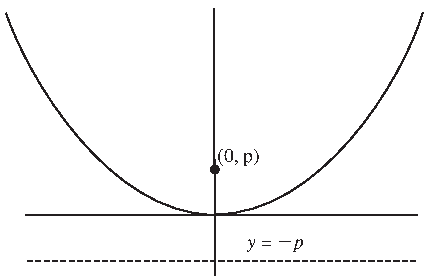
\includegraphics[width=0.586\linewidth,height=.8\textheight,keepaspectratio]{assets/p324_04.pdf}\end{center}
\end{BookFloat}

Care must be taken in deciding the order for the indeterminate. In Example 38.6, had we taken the order of the indeterminates to be \BookInline{d<p<x<y,\allowbreak } the resulting Gröbner basis would have been \BookInline{\{- 4dp+ 4p^{2}+ x^{2},\allowbreak d- p- y\},\allowbreak } which does not directly give the standard form for the equation of a parabola. The reason for making the indeterminate \BookInline{d} the largest is that the algorithm attempts to eliminate \BookInline{d} from polynomials in the basis since the reduction process reduces the maximum-sized term.

The algorithm for computing Gröbner bases can be programmed. In fact, it is a built-in function on many common mathematical packages including Mathematica, Maple, Wolfram Alpha, and others. By carefully picking the order of the indeterminates, it is possible to solve a large variety of problems using automated computations of Gröbner bases.

\BookLabel{38.7 Example} We use a software package to compute a Gröbner basis that yields the equation of an ellipse in standard position. An ellipse in standard position is the set of all points in the plane so that the sum of the distances to the two foci \BookInline{(c,\allowbreak 0)} and \BookInline{(- c,\allowbreak 0)} is a fixed distance \BookInline{2a.} We start with the basis

\begin{center}\begin{adjustbox}{max width=\linewidth}\BookInline{\displaystyle \{(x- c)^{2}+ y^{2}- d_{1}^{2},\allowbreak (x+ c)^{2}+ y^{2}- d_{2}^{2},\allowbreak d_{1}+ d_{2}- 2a\}}\end{adjustbox}\end{center}

\noindent where \BookInline{d_{1}} represents the distance to focus \BookInline{(c,\allowbreak 0)} and \BookInline{d_{2}} represents the distance to focus \BookInline{(- c,\allowbreak 0).} We wish to arrive at a polynomial that includes \BookInline{x} and \BookInline{y} as well as the parameters \BookInline{a} and \BookInline{c} that describe the shape and size of the ellipse. Therefore, we take \BookInline{d_{1}} and \BookInline{d_{2}} as the largest indeterminates. Using the order \BookInline{a<c<y<x<d_{2}<d_{1},\allowbreak } a mathematical software package quickly computes the Gröbner basis

\begin{center}\begin{adjustbox}{max width=\linewidth}\BookInline{\displaystyle \{a^{4}- a^{2}c^{2}- a^{2}x^{2}+ c^{2}x^{2}- a^{2}y^{2},\allowbreak - a^{2}+ ad_{2}- cx,\allowbreak a^{3}- ac^{2}- acs+ cd_{2}x- ax^{2}- ay^{2},\allowbreak }\end{adjustbox}\end{center}

\begin{center}\begin{adjustbox}{max width=\linewidth}\BookInline{\displaystyle - c^{2}+ d_{2}^{2}- 2cx- x^{2}- y^{2},\allowbreak - 2a+ d_{1}+ d_{2}\}.}\end{adjustbox}\end{center}

\end{BookBody}

% Source PDF page 325; original printed page 308
\BookSource{325}{308}
\BookNarrativetrue

\begin{BookBody}

\noindent The first polynomial can be written as

\begin{center}\begin{adjustbox}{max width=\linewidth}\BookInline{\displaystyle a^{2}(a^{2}- c^{2})- (a^{2}- c^{2})x^{2}- a^{2}y^{2}.}\end{adjustbox}\end{center}

\noindent We think of \BookInline{a} and \BookInline{c} as parameters and recall that in an ellipse, the parameter \BookInline{b>0} is defined by \BookInline{b^{2}= a^{2}- c^{2}.} We see that the variety in \BookInline{\mathbb{R}^{2}} defined from the ideal \BookInline{\langle a^{2}b^{2}- } \BookInline{b^{2}x^{2}- a^{2}y^{2}\rangle } has equation

\begin{center}\begin{adjustbox}{max width=\linewidth}\BookInline{\displaystyle { \frac { x ^ { 2 } } { a ^ { 2 } } } + { \frac { y ^ { 2 } } { b ^ { 2 } } } = 1 .}\end{adjustbox}\end{center} \BookEnd{\blacktriangle}

A\textbf{ graph} is a finite set with elements called\textbf{ vertices} together with a collection of pairs of vertices called\textbf{ edges} or\textbf{ arcs}. Graphs are often drawn as in Figure 38.10, which shows a graph with four vertices \BookInline{x_{1},\allowbreak x_{2},\allowbreak x_{3},\allowbreak x_{4}} and four edges \BookInline{\{x_{1},\allowbreak x_{2}\},\allowbreak \{x_{2},\allowbreak x_{3}\},\allowbreak \{x_{3},\allowbreak x_{1}\},\allowbreak } \BookInline{\{x_{3},\allowbreak x_{4}\}.} A\textbf{ coloring} of a graph is an assignment of colors to the vertices in such a way that no two vertices in the same edge have the same color. The problem of determining if a graph can be colored with \BookInline{n} colors can be restated as a question about an ideal, which can (at least theoretically) be answered using Gröbner bases.

\BookLabel{38.8 Theorem} Let \BookInline{G} be a graph with vertex set \BookInline{\{x_{1},\allowbreak x_{2},\allowbreak...,\allowbreak x_{k}\}.} We identify each vertex with an indeterminate and form the ideal \BookInline{I\subseteq \mathbb{C}[x_{1},\allowbreak x_{2},\allowbreak...,\allowbreak x_{k}]} with basis consisting of polynomials \BookInline{x_{1}- 1,\allowbreak x_{2}^{n}- 1,\allowbreak x_{3}^{n}- 1,\allowbreak...,\allowbreak x_{k}^{n}- 1} together with a polynomial \BookInline{x}\textit{in}\BookInline{- 1+ x}\textit{in}\BookInline{- 2xj+ x}\textit{in}\BookInline{- 3xj2+ } \BookInline{\cdots + x_{i}x_{j}^{n- 2}+ x_{j}^{n- 1}} for each edge in the graph. The graph \BookInline{G} can be colored with \BookInline{n} colors if and only if the algebraic variety \BookInline{V(I)} is nonempty.

\BookLabel{\textit{Proof}} The proof is left for Exercise 34. \BookEnd{\blacklozenge}

The variety \BookInline{V(I)} in Theorem 38.8 gives all possible colorings of the graph \BookInline{G} using the \BookInline{n ^ { \mathrm { t h } }} roots of unity for the colors and coloring vertex \BookInline{x_{1}} with the color 1. For each point in \BookInline{V(I),\allowbreak } the \BookInline{j ^ { \mathrm { t h } }} coordinate gives the color assigned to \BookInline{x_{j}.}

\BookLabel{38.9 Example} Using the graph in Figure 38.10, the basis described in Theorem 38.8 for \BookInline{n= 2} is

\begin{center}\begin{adjustbox}{max width=\linewidth}\BookInline{\displaystyle \{x_{1}- 1,\allowbreak x_{2}^{2}- 1,\allowbreak x_{3}^{2}- 1,\allowbreak x_{4}^{2}- 1,\allowbreak x_{1}+ x_{2},\allowbreak x_{2}+ x_{3},\allowbreak x_{3}+ x_{1},\allowbreak x_{3}+ x_{4}\}.}\end{adjustbox}\end{center}

\noindent A Gröbner basis is \BookInline{\{1\}.} This can be determined electronically, or by noticing that

\begin{center}\begin{adjustbox}{max width=\linewidth}\BookInline{\displaystyle (x_{1}+ x_{2})- (x_{2}+ x_{3})+ (x_{3}+ x_{1})= 2x_{1}\in I.}\end{adjustbox}\end{center}

\noindent Therefore\BookInline{,\allowbreak x_{1}\in I,\allowbreak } so \BookInline{x_{1}- (x_{1}- 1)= 1\in I.} Thus the ideal is all of \BookInline{\mathbb{C}[x_{1},\allowbreak x_{2},\allowbreak x_{3},\allowbreak x_{4}],\allowbreak } which has \BookInline{\{1\}} as a basis. Since the algebraic variety for \BookInline{\langle 1\rangle } is the empty set, the graph cannot be colored with two colors.

We now compute a Gröbner basis when \BookInline{n= 3.} Theorem 38.8 tells us to start with the basis

\begin{BookFloat}{38_gr_bner_bases_for_ideals-p325-16}
\begin{center}\small \textbf{38.10 Figure}\end{center}
\begin{center}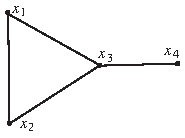
\includegraphics[width=0.254\linewidth,height=.8\textheight,keepaspectratio]{assets/review_v3_p325_38.10.pdf}\end{center}
\end{BookFloat}

\begin{center}\begin{adjustbox}{max width=\linewidth}\BookInline{\displaystyle \begin{aligned}&\{x_{1}- 1,\allowbreak x_{2}^{3}- 1,\allowbreak x_{3}^{3}- 1,\allowbreak x_{4}^{3}- 1,\allowbreak x_{1}^{2}+ x_{1}x_{2}+ x_{2}^{2},\allowbreak x_{2}^{2}+ x_{2}x_{3}+ x_{3}^{2},\allowbreak x_{3}^{2}+ x_{3}x_{1} \\ &+ x_{1}^{2},\allowbreak x_{3}^{2}+ x_{3}x_{4}+ x_{4}^{2}\}.\end{aligned}}\end{adjustbox}\end{center}

\noindent Using a software package, a Gröbner basis with indeterminate order \BookInline{x_{1}<x_{2}<x_{3}<x_{4}} is

\begin{center}\begin{adjustbox}{max width=\linewidth}\BookInline{\displaystyle \{x_{1}- 1,\allowbreak x_{2}^{2}+ x_{2}+ 1,\allowbreak 1+ x_{2}+ x_{3},\allowbreak x_{2}- x_{4}- x_{2}x_{4}+ x_{4}^{2}\}.}\end{adjustbox}\end{center}

\noindent Let $\zeta=-\frac{\sqrt{3}}{2}+\frac{1}{2}i$ be a third root of unity. We find an element $(a_1,a_2,a_3,a_4)\in V(I)$:
% The printed source has -sqrt(3)/2 + i/2 here. This is retained faithfully;
% it is a source erratum (a cube root would instead be -1/2 + sqrt(3)i/2).
\[
\begin{aligned}
a_1-1 &= 0 && a_1=1,\\
a_2^2+a_2+1 &= 0 && \begin{aligned}[t]
 &\text{$a_2$ is a third root of unity.}\\
 &\text{Let }a_2=\zeta.
 \end{aligned}\\
1+\zeta+a_3 &= 0 && a_3=-1-\zeta=\zeta^2,\\
\zeta-a_4-\zeta a_4+a_4^2 &= 0 && \begin{aligned}[t]
 &\text{factoring,}\\
 &(\zeta-a_4)(1-a_4)=0.
 \end{aligned}
\end{aligned}
\]

\end{BookBody}

% Source PDF page 326; original printed page 309
\BookSource{326}{309}
\BookNarrativetrue

\begin{BookBody}

\noindent We see that we can color vertex 1 the color 1, vertex \BookInline{2\zeta,\allowbreak } vertex \BookInline{3\zeta ^{2},\allowbreak } and then we can color vertex 4 either the color 1 or \BookInline{\zeta.}\BookEnd{\blacktriangle}

There are many applications of Gröbner bases in mathematics, statistics, engineering, and computer science. These include controlling robot arms and automated theorem proving. The algorithm to compute a Gröbner basis is generally too long and tedious to be done by hand, so computers are essential. However, some larger problems are not feasible even on modern high-speed computers.

\end{BookBody}

\BookNarrativefalse

\begin{BookBody}

\BookExerciseTitle{38}

\noindent In Exercises 1 through 4, write the polynomials in \BookInline{\mathbb{R}[x,\allowbreak y,\allowbreak z]} in decreasing term order, using the order lex for power products \BookInline{x^{m}y^{n}z^{s}} where \BookInline{z<y<x.}

\BookExercise{1.}{\BookInline{2xy^{3}z^{5}- 5x^{2}yz^{3}+ 7x^{2}y^{2}z- 3x^{3}}}

\BookExercise{2.}{\BookInline{3y^{2}z^{5}- 4x+ 5y^{3}z^{3}- 8z^{7}}}

\BookExercise{3.}{\BookInline{3y- 7x+ 10z^{3}- 2xy^{2}z^{2}+ 2x^{2}yz^{2}}}

\BookExercise{4.}{\BookInline{38- 4xz+ 2yz- 8xy+ 3yz^{3}}}

\noindent In Exercises 5 through 8, write the polynomials in \BookInline{\mathbb{R}[x,\allowbreak y,\allowbreak z]} in decreasing term order, using the order lex for power products \BookInline{z^{m}y^{n}x^{s}} where \BookInline{x<y<z.}

\BookExercise{5.}{The polynomial in Exercise 1.}

\BookExercise{6.}{The polynomial in Exercise 2.}

\BookExercise{7.}{The polynomial in Exercise 3.}

\BookExercise{8.}{The polynomial in Exercise 4.}

\noindent Another ordering, deglex, for power products in \BookInline{F[}\textbf{x}] is defined as follows:

\begin{center}\begin{adjustbox}{max width=\linewidth}\BookInline{\displaystyle x_{1}^{s_{1}}x_{2}^{s_{2}}\cdots x_{n}^{s_{n}}<x_{1}^{t_{1}}x_{2}^{t_{2}}\cdots x_{n}^{t_{n}}}\end{adjustbox}\end{center}

\noindent if and only if either \BookInline{\sum _{i= 1}^{n}s_{i}<\sum _{i= 1}^{n}t_{i},\allowbreak } or these two sums are equal and \BookInline{s_{i}<t_{i}} for the smallest value of \BookInline{i} such that \BookInline{s_{i}\neq t_{i}.} Exercises 9 through 13 are concerned with the order deglex.

\BookExercise{9.}{List, in increasing order, the smallest 20 power products in \BookInline{\mathbb{R}[x,\allowbreak y,\allowbreak z]} for the order deglex with power products \BookInline{x^{m}y^{n}z^{s}} where \BookInline{z<y<x.}}

\noindent In Exercises 10 through 13, write the polynomials in order of decreasing terms using the order deglex with power products \BookInline{x^{m}y^{n}z^{s}} where \BookInline{z<y<x.}

\BookExercise{10.}{The polynomial in Exercise 1.}

\BookExercise{11.}{The polynomial in Exercise 2.}

\BookExercise{12.}{The polynomial in Exercise 3.}

\BookExercise{13.}{The polynomial in Exercise 4.}

\noindent For Exercises 14 through 17, let power products in \BookInline{\mathbb{R}[x,\allowbreak y,\allowbreak z]} have order lex where \BookInline{z<y<x.} If possible, perform a single-step division algorithm reduction that changes the given ideal basis to one having smaller maximum term order.

\BookExercise{14.}{\BookInline{\langle xy^{2}- 2x,\allowbreak x^{2}y+ 4xy,\allowbreak xy- y^{2}\rangle }}

\BookExercise{15.}{\BookInline{\langle xy+ y^{3},\allowbreak y^{3}+ z,\allowbreak x- y^{4}\rangle }}

\BookExercise{16.}{\BookInline{\langle xyz- 3z^{2},\allowbreak x^{3}+ y^{2}z^{3},\allowbreak x^{2}yz^{3}+ 4\rangle }}

\BookExercise{17.}{\BookInline{\langle y^{2}z^{3}+ 3,\allowbreak y^{3}z^{2}- 2z,\allowbreak y^{2}z^{2}+ 3\rangle }}

\noindent In Exercises 18 and 19, let the order of power products in \BookInline{\mathbb{R}[w,\allowbreak x,\allowbreak y,\allowbreak z]} be lex with \BookInline{z<y<x<w.} Find a Gröbner basis for the given ideal.

\begin{center}\begin{adjustbox}{max width=\linewidth}\BookInline{\displaystyle 18.\langle w+ x- y+ 4z- 3,\allowbreak 2w+ x+ y- 2z+ 4,\allowbreak w+ 3x- 3y+ z- 5\rangle}\end{adjustbox}\end{center}

\BookExercise{19.}{\BookInline{\langle w- 4x+ 3y- z+ 2,\allowbreak 2w- 2x+ y- 2z+ 5,\allowbreak w- 10x+ 8y- z- 1\rangle }}

\noindent In Exercises 20 through 22, find a Gröbner basis for the indicated ideal in \BookInline{\mathbb{R}[x].}

\BookExercise{20.}{\BookInline{\langle x^{4}+ x^{3}- 3x^{2}- 4x- 4,\allowbreak x^{3}+ x^{2}- 4x- 4\rangle }}

\BookExercise{21.}{\BookInline{\langle x^{4}- 4x^{3}+ 5x^{2}- 2x,\allowbreak x^{3}- x^{2}- 4x+ 4,\allowbreak x^{3}- 3x+ 2\rangle }}

\BookExercise{22.}{\BookInline{\langle x^{5}+ x^{2}+ 2x- 5,\allowbreak x^{3}- x^{2}+ x- 1\rangle }}

\noindent In Exercises 23 through 26, find a Gröbner basis for the given ideal in \BookInline{\mathbb{R}[x,\allowbreak y].} Consider the order of power products to be lex with \BookInline{y<x.} If you can, describe the corresponding algebraic variety in \BookInline{\mathbb{R}[x,\allowbreak y].}

\end{BookBody}

% Source PDF page 327; original printed page 310
\BookSource{327}{310}
\BookNarrativefalse

\begin{BookBody}

\BookExercise{23.}{\BookInline{\langle x^{2}y- x- 2,\allowbreak xy+ 2y- 9\rangle }}

\BookExercise{24.}{\BookInline{\langle x^{2}y+ x,\allowbreak xy^{2}- y\rangle }}

\BookExercise{25.}{\BookInline{\langle x^{2}y+ x+ 1,\allowbreak xy^{2}+ y- 1\rangle }}

\BookExercise{26.}{\BookInline{\langle x^{2}y+ xy^{2},\allowbreak xy- x\rangle }}

\BookTextHeading{\textbf{Concepts}}

\BookExercise{27.}{Determine whether each of the following is true or false.}

\BookExercise{a.}{Polynomials in a Gröbner basis are linearly independent.}

\BookExercise{b.}{The set \BookInline{\{1\}} is a Gröbner basis.}

\BookExercise{c.}{The set \BookInline{\{0\}} is a Gröbner basis.}

\BookExercise{d.}{The order one picks for the power products does not affect the resulting Gröbner basis.}

\BookExercise{e.}{For any total ordering of all the power products\BookInline{,\allowbreak x_{1}^{2}>x_{1}.}}

\BookExercise{f.}{A Gröbner basis can be used to determine if a graph can be colored with \BookInline{n} colors starting with a basis consisting of polynomials each of degree at most \BookInline{n.}}

\BookExercise{g.}{A Gröbner basis can be used to determine if a graph can be colored with \BookInline{n} colors starting with a basis consisting of \BookInline{r+ s} polynomials where \BookInline{r} is the number of vertices in the graph and \BookInline{s} is the number of edges in the graph.}

\BookExercise{h.}{I have computed Gröbner bases before I knew what they were.}

\BookExercise{i.}{Any ideal in \BookInline{F[}\textbf{x}] has a unique Gröbner basis.}

\BookExercise{j.}{A basis for an ideal \BookInline{I} in \BookInline{F[x_{1},\allowbreak x_{2},\allowbreak...,\allowbreak x_{n}]} is a Gröbner basis if and only if each polynomial in the basis cannot be reduced further using the division algorithm.}

\BookExercise{28.}{Let \BookInline{\mathbb{R}[x,\allowbreak y]} be ordered by lex. Give an example to show that \BookInline{P_{i}<P_{j}} does not imply that \BookInline{P_{i}} divides \BookInline{P_{j}.}}

\BookExercise{29.}{What other orders of the indeterminate \BookInline{a,\allowbreak c,\allowbreak x,\allowbreak y,\allowbreak d_{1},\allowbreak d_{2}} would you expect the equation of an ellipse to result from computing a Gröbner basis for the ideal in Example 38.7?}

\BookExercise{30.}{Use a Gröbner basis to derive the formula for a hyperbola in standard position. Recall that a hyperbola in standard position is the set of all points in the plane whose difference in distances from \BookInline{(c,\allowbreak 0)} and \BookInline{(- c,\allowbreak 0)} is \BookInline{\pm 2a.} You may use a computer to compute the Gröbner basis.}

\BookExercise{31.}{Use a Gröbner basis to show that the graph with vertex set \BookInline{\{x_{1},\allowbreak x_{2},\allowbreak x_{3},\allowbreak x_{4},\allowbreak x_{5}\}} and edge set \BookInline{\{\{x_{1},\allowbreak x_{2}\},\allowbreak \{x_{2},\allowbreak x_{3}\},\allowbreak } \BookInline{\{x_{3},\allowbreak x_{4}\},\allowbreak \{x_{1},\allowbreak x_{3}\},\allowbreak \{x_{1},\allowbreak x_{5}\},\allowbreak \{x_{5},\allowbreak x_{4}\}\}} cannot be colored with three colors, but it can be colored with four colors. You may use a computer to compute the Gröbner basis.}

\BookTextHeading{\textbf{Theory}}

\BookExercise{32.}{Show that \BookInline{\{xy,\allowbreak y^{2}- y)} is a Gröbner basis for \BookInline{\langle xy,\allowbreak y^{2}- y\rangle,\allowbreak } as asserted after Example 38.1.}

\BookExercise{33.}{Show that \BookInline{\{- 4yp+ x^{2},\allowbreak d- y- p\}} is a Gröbner basis for the ideal \BookInline{\langle - 4yp+ x^{2},\allowbreak d- y- p\rangle } as asserted in Example 38.6.}

\BookExercise{34.}{Prove Theorem 38.8. [Hint: Think about coloring a graph with the \BookInline{n ^ { \mathrm { t h } }} roots of unity.]}

\end{BookBody}
\ifdefined\BookMaster\let\BookFinish\relax\else\def\BookFinish{\end{document}}\fi\BookFinish

\clearpage
% !TeX program = xelatex
\ifdefined\BookMaster\else
\documentclass[11pt,oneside]{article}
% !TeX program = xelatex
\usepackage[b5paper,left=22mm,right=22mm,top=20mm,bottom=22mm,footskip=11mm]{geometry}
\usepackage{fontspec}
\setmainfont{TeX Gyre Termes}
\setsansfont{TeX Gyre Heros}
\usepackage{amsmath,amssymb,mathtools,amsthm}
\renewcommand{\cdots}{\mathinner{\cdotp\cdotp\cdotp}}
\usepackage{graphicx,adjustbox,array,booktabs,longtable,multirow,enumitem,changepage,needspace}
\usepackage[table]{xcolor}
\usepackage{fancyhdr}
\raggedbottom
\interfootnotelinepenalty=10000
\newcommand{\BookFootnote}[2]{\begingroup\renewcommand{\thefootnote}{\fnsymbol{footnote}}\footnote[#1]{#2}\endgroup}
\newcommand{\BookFootnoteMark}[1]{\begingroup\renewcommand{\thefootnote}{\fnsymbol{footnote}}\footnotemark[#1]\endgroup}
\newcommand{\BookFootnoteText}[2]{\begingroup\renewcommand{\thefootnote}{\fnsymbol{footnote}}\footnotetext[#1]{#2}\endgroup}
\newenvironment{BookFloat}[1]{\par\addvspace{.6\baselineskip}\noindent\def\BookFloatID{#1}\begin{minipage}{\linewidth}\phantomsection\label{bookfloat:#1:start}}{\phantomsection\label{bookfloat:\BookFloatID:end}\end{minipage}\par\addvspace{.6\baselineskip}}

\usepackage[unicode,hidelinks]{hyperref}
\pagestyle{fancy}
\fancyhf{}
\newcommand{\BookFooter}{}
\fancyfoot[L]{\parbox[b]{\dimexpr\textwidth-15mm}{\footnotesize\BookFooter}}
\fancyfoot[R]{\footnotesize\thepage}
\renewcommand{\headrulewidth}{0pt}
\renewcommand{\footrulewidth}{0pt}
\setlength{\parindent}{0pt}
\setlength{\parskip}{0.2em}
\setlength{\emergencystretch}{3em}
\setlist{nosep,leftmargin=1.7em,labelsep=.65em}
\newif\ifBookNarrative
\BookNarrativetrue
\newenvironment{BookBody}{\setlength{\parindent}{0pt}}{}
\newcommand{\BookStatement}[1]{\par\addvspace{.6\baselineskip}\noindent #1\enspace\ignorespaces}
\newcommand{\BookLabel}[1]{\par\addvspace{.6\baselineskip}\needspace{3\baselineskip}\noindent\textbf{#1}\quad\ignorespaces}
\newcommand{\BookHeading}[1]{\par\addvspace{\baselineskip}\needspace{4\baselineskip}\noindent{\large\bfseries #1}\par\medskip}
\newcommand{\BookSubheading}[1]{\par\addvspace{.7\baselineskip}\needspace{3\baselineskip}\noindent{\bfseries #1}\par\smallskip}
\newcommand{\BookTextHeading}[1]{\par\addvspace{.7\baselineskip}\needspace{3\baselineskip}\noindent #1\par\smallskip}
\newcommand{\BookSectionTitle}[2]{\par\addvspace{1.2\baselineskip}\needspace{5\baselineskip}\noindent\colorbox{gray!25}{\sffamily\bfseries\small SECTION #1}\quad{\large\bfseries #2}\par\medskip}
\newcommand{\BookExerciseTitle}[1]{\par\addvspace{\baselineskip}\needspace{4\baselineskip}\noindent{\color{gray}\rule{1.5mm}{1.5mm}}\enspace{\large\bfseries Exercises #1}\par\medskip}
\newcommand{\BookBullet}[1]{\begin{list}{\textbullet}{\setlength{\leftmargin}{1.7em}\setlength{\labelwidth}{1em}\setlength{\labelsep}{.7em}\setlength{\topsep}{0pt}\setlength{\parsep}{0pt}\setlength{\itemsep}{0pt}}\item #1\end{list}}
\newcommand{\BookExercise}[2]{\begin{list}{\textbf{#1}}{\setlength{\leftmargin}{2.2em}\setlength{\labelwidth}{1.5em}\setlength{\labelsep}{.7em}\setlength{\topsep}{.15em}\setlength{\parsep}{0pt}\setlength{\itemsep}{0pt}}\item #2\end{list}}
\newcommand{\BookEnd}[1]{\unskip\nobreak\hfill\ensuremath{#1}}
\newcommand{\BookSource}[2]{\phantomsection\label{sourcepage:#1}} % Source-page anchors, retained through reflow.
\usepackage{multicol}
\usepackage{tikz}
\newcommand{\BookPartEntry}[2]{\par\noindent\makebox[17mm][l]{\bfseries Section #1}#2\par}
\newcommand{\BookPartTitle}[3]{\par\bigskip\noindent\begin{tikzpicture}\node[anchor=north west,inner sep=0pt,outer sep=0pt] (bookpart) at (0,0) {\begin{minipage}{\dimexpr\linewidth-.5pt}\hspace*{26mm}\begin{minipage}[t]{\dimexpr\linewidth-26mm}\begin{adjustbox}{max width=\linewidth}{\fontsize{20}{24}\selectfont\bfseries #2}\end{adjustbox}\par\vspace{6mm}\hrule\vspace{6mm}{\sffamily\footnotesize\setlength{\parskip}{.3em}#3}\vspace{3mm}\end{minipage}\end{minipage}};\path[shade,top color=gray!60,bottom color=white] (0,0) rectangle ([xshift=24mm]bookpart.south west);\node[anchor=north,font=\sffamily\bfseries\small] at (12mm,-2mm) {PART};\node[anchor=north,font=\sffamily\bfseries\Huge] at (12mm,-7mm) {#1};\end{tikzpicture}\par\bigskip}
\newsavebox{\BookMathBox}
\makeatletter
\newcommand{\BookInline}[1]{\leavevmode\hskip0pt\relax\begingroup\in@{\begin}{#1}\ifin@\sbox{\BookMathBox}{\(#1\)}\ifdim\wd\BookMathBox>\dimexpr\linewidth-1em\relax\resizebox{\dimexpr\linewidth-1em\relax}{!}{\usebox{\BookMathBox}}\else\(#1\)\fi\else\in@{\left}{#1}\ifin@\sbox{\BookMathBox}{\(#1\)}\ifdim\wd\BookMathBox>\dimexpr\linewidth-1em\relax\resizebox{\dimexpr\linewidth-1em\relax}{!}{\usebox{\BookMathBox}}\else\(#1\)\fi\else\(#1\)\fi\fi\endgroup\hskip0pt\relax}
\makeatother
\DeclareMathOperator{\Aut}{Aut}
\DeclareMathOperator{\End}{End}
\DeclareMathOperator{\Hom}{Hom}
\DeclareMathOperator{\GF}{GF}
\DeclareMathOperator{\irr}{irr}
\DeclareMathOperator{\lt}{lt}
\DeclareMathOperator{\lp}{lp}
\providecommand{\textcircled}[1]{\textnormal{(#1)}}

\begin{document}
\fi
\renewcommand{\BookFooter}{Section 39 Introduction to Extension Fields}
\pdfbookmark[0]{Section 39 Introduction to Extension Fields}{39_introduction_to_extension_fields}
\ifdefined\BookMaster\else\setcounter{page}{311}\fi
% Source PDF page 328; original printed page 311
\BookSource{328}{311}
\BookPartTitle{VIII}{Extension Fields}{\BookPartEntry{39}{Introduction to Extension Fields}
\BookPartEntry{40}{Algebraic Extensions}
\BookPartEntry{41}{Geometric Constructions\label{bookfootnote:328:2:ref}\BookFootnoteMark{2}}
\BookPartEntry{42}{Finite Fields}}
\BookFootnoteText{2}{\label{bookfootnote:328:2:text}Section 41 is not required for the remainder of the text.}

\BookNarrativetrue

\begin{BookBody}

\BookSectionTitle{39}{Introduction to Extension Fields}

\BookTextHeading{\textbf{Our Basic Goal Achieved}  }

\noindent We are now in a position to achieve our\textbf{ basic goal,} which, loosely stated, is to show that every nonconstant polynomial has a zero. This will be stated more precisely and proved in Theorem 39.3. We first introduce some new terminology for some old ideas.

\BookLabel{39.1 Definition} A field \BookInline{E} is an\textbf{ extension field of a field} \BookInline{F} if \BookInline{F\leq E.} \BookEnd{\blacksquare}

\begin{BookFloat}{39_introduction_to_extension_fields-p328-12}
\begin{center}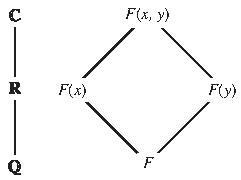
\includegraphics[width=0.331\linewidth,height=.8\textheight,keepaspectratio]{assets/p328_10.pdf}\end{center}
\begin{center}\small\textbf{39.2 Figure}\end{center}
\end{BookFloat}

Thus \BookInline{\mathbb{R}} is an extension field of \BookInline{\mathbb{Q},\allowbreak } and \BookInline{\mathbb{C}} is an extension field of both \BookInline{\mathbb{R}} and \BookInline{\mathbb{Q}.} As in the study of groups, it will often be convenient to use subfield diagrams to picture extension fields, the larger field being on top. We illustrate this in Fig. 39.2. (Recall that \BookInline{F(x)} is the field of quotients constructed from \BookInline{F[x].)} A configuration where there is just one single column of fields, as at the left-hand side of Fig. 39.2, is often referred to, without any precise definition, as a\textbf{ tower of fields.}

Now for our\textit{ basic goal!} This great and important result follows quickly and elegantly from the techniques we now have at our disposal.

\end{BookBody}

% Source PDF page 329; original printed page 312
\BookSource{329}{312}
\BookNarrativetrue

\begin{BookBody}

\BookLabel{39.3 Theorem} \textbf{(Kronecker’s Theorem) (Basic Goal)} Let \BookInline{F} be a field and let \BookInline{f(x)} be a nonconstant polynomial in \BookInline{F[x].} Then there exists an extension field \BookInline{E} of \BookInline{F} and an \BookInline{\alpha \in E} such that \BookInline{f(\alpha )= 0.}

\BookLabel{\textit{Proof}} By Theorem \BookInline{28.21,\allowbreak f(x)} has a factorization in \BookInline{F[x]} into polynomials that are irreducible over \BookInline{F.} Let \BookInline{p(x)} be an irreducible polynomial in such a factorization. It is clearly sufficient to find an extension field \BookInline{E} of \BookInline{F} containing an element \BookInline{\alpha } such that \BookInline{p(\alpha )= 0.}

By Theorem \BookInline{31.25,\allowbreak \langle p(x)\rangle } is a maximal ideal in \BookInline{F[x],\allowbreak } so \BookInline{F[x]/\langle p(x)\rangle } is a field. We claim that \BookInline{F} can be identified with a subfield of \BookInline{F[x]/\langle p(x)\rangle } in a natural way by use of the map \BookInline{\psi:F\to F[x]/\langle p(x)\rangle } given by

\begin{center}\begin{adjustbox}{max width=\linewidth}\BookInline{\displaystyle \psi (a)= a+ \langle p(x)\rangle}\end{adjustbox}\end{center}

\noindent for \BookInline{a\in F.} This map is one-to-one, for if \BookInline{\psi (a)= \psi (b),\allowbreak } that is, if \BookInline{a+ \langle p(x)\rangle = b+ \langle p(x)\rangle } for some \BookInline{a,\allowbreak b\in F,\allowbreak } then \BookInline{(a- b)\in \langle p(x)\rangle,\allowbreak } so \BookInline{a- b} must be a multiple of the polynomial \BookInline{p(x),\allowbreak } which is of degree \BookInline{\geq 1.} Now \BookInline{a,\allowbreak b\in F} implies that \BookInline{a- b} is in \BookInline{F.} Thus we must have \BookInline{a- b= 0,\allowbreak } so \BookInline{a= b.} We defined addition and multiplication in \BookInline{F[x]/\langle p(x)\rangle } by choosing any representatives, so we may choose \BookInline{a\in (a+ \langle p(x)\rangle ).} Thus \BookInline{\psi } is a homomorphism that maps \BookInline{F} one-to-one onto a subfield of \BookInline{F[x]/\langle p(x)\rangle.} We identify \BookInline{F} with \BookInline{\{a+ \langle p(x)\rangle \mid a\in F\}} by means of this map \BookInline{\psi.} Thus we shall view \BookInline{E= F[x]/\langle p(x)\rangle } as an extension field of \BookInline{F.} We have now manufactured our desired extension field \BookInline{E} of \BookInline{F.} It remains for us to show that \BookInline{E} contains a zero of \BookInline{p(x).}

\BookTextHeading{\textbf{HISTORICAL NOTE}  } \BookEnd{\blacksquare}

\noindent Leopold Kronecker is known for his insistence on constructibility of mathematical objects. As he noted, “God made the integers; all else is the work of man.” Thus, he wanted to be able to construct new “domains of rationality” (fields) by using only the existence of integers and indeterminates. He did not believe in starting with the real or complex numbers, because as far as he was concerned, those fields could not be determined in a constructive way. Hence in an 1881 paper, Kronecker created an extension field by simply adjoining to a given field a root \BookInline{\alpha } of an irreducible \BookInline{n}th degree polynomial \BookInline{p(x);} that is, his new field consisted of expressions rational in the original field elements and his new root \BookInline{\alpha } with the condition that \BookInline{p(\alpha )= 0.} The proof of the theorem presented in the text (Theorem 39.3) dates from the twentieth century.

Kronecker completed his dissertation in 1845 at the University of Berlin. For many years thereafter, he managed the family business, ultimately becoming financially independent. He then returned to Berlin, where he was elected to the Academy of Sciences and thus permitted to lecture at the university. On the retirement of Kummer, he became a professor at Berlin, and with Karl Weierstrass (1815–1897) directed the influential mathematics seminar.

Let us set

\begin{center}\begin{adjustbox}{max width=\linewidth}\BookInline{\displaystyle \alpha = x+ \langle p(x)\rangle ,\allowbreak }\end{adjustbox}\end{center}

\noindent so \BookInline{\alpha \in E.} Consider the evaluation homomorphism \BookInline{\phi _{\alpha }:F[x]\to E,\allowbreak } given by Theorem 27.4. If \BookInline{p(x)= a_{0}+ a_{1}x+ \cdots + a_{n}x^{n},\allowbreak } where \BookInline{a_{i}\in F,\allowbreak } then we have

\begin{center}\begin{adjustbox}{max width=\linewidth}\BookInline{\displaystyle \phi _{\alpha }(p(x))= a_{0}+ a_{1}(x+ \langle p(x)\rangle )+ \cdots + a_{n}(x+ \langle p(x)\rangle )^{n}}\end{adjustbox}\end{center}

\noindent in \BookInline{E= F[x]/\langle p(x)\rangle.} \textit{But we can compute in} \BookInline{F[x]/\langle p(x)\rangle } \textit{by choosing representatives, and} \BookInline{x} \textit{is} \BookInline{a} \textit{representative of the coset} \BookInline{\alpha = x+ \langle p(x)\rangle.} Therefore,

\begin{center}\begin{adjustbox}{max width=\linewidth}\BookInline{\displaystyle \begin{aligned}p(\alpha) &= \left( a_{0} + a_{1}x + \cdots + a_{n}x^{n} \right) + \langle p(x) \rangle \\&= p(x) + \langle p(x) \rangle = \langle p(x) \rangle = 0\end{aligned}}\end{adjustbox}\end{center}

\end{BookBody}

% Source PDF page 330; original printed page 313
\BookSource{330}{313}
\BookNarrativetrue

\begin{BookBody}

\noindent in \BookInline{F[x]/\langle p(x)\rangle.} We have found an element \BookInline{\alpha } in \BookInline{E= F[x]/\langle p(x)\rangle } such that \BookInline{p(\alpha )= 0,\allowbreak } and therefore \BookInline{f(\alpha )= 0.}\BookEnd{\blacklozenge}

We illustrate the construction involved in the proof of Theorem 39.3 by two examples.

\BookLabel{39.4 Example} Let \BookInline{F= \mathbb{R},\allowbreak } and let \BookInline{f(x)= x^{2}+ 1,\allowbreak } which is well known to have no zeros in \BookInline{\mathbb{R}} and thus is irreducible over \BookInline{\mathbb{R}} by Theorem 28.11. Then \BookInline{\langle x^{2}+ 1\rangle } is a maximal ideal in \BookInline{\mathbb{R}[x],\allowbreak } so \BookInline{\mathbb{R}[x]/\langle x^{2}+ 1\rangle } is a field. Identifying \BookInline{r\in \mathbb{R}} with \BookInline{r+ \langle x^{2}+ 1\rangle } in \BookInline{\mathbb{R}[x]/\langle x^{2}+ 1\rangle,\allowbreak } we can view \BookInline{\mathbb{R}} as a subfield of \BookInline{E= \mathbb{R}[x]/\langle x^{2}+ 1\rangle.} Let

\begin{center}\begin{adjustbox}{max width=\linewidth}\BookInline{\displaystyle \alpha = x+ \langle x^{2}+ 1\rangle .}\end{adjustbox}\end{center}

Computing in \BookInline{\mathbb{R}[x]/\langle x^{2}+ 1\rangle,\allowbreak } we find

\begin{center}\begin{adjustbox}{max width=\linewidth}\BookInline{\displaystyle \begin{aligned}\alpha ^{2}+ 1&= (x+ \langle x^{2}+ 1\rangle )^{2}+ (1+ \langle x^{2}+ 1\rangle ) \\ &= (x^{2}+ 1)+ \langle x^{2}+ 1\rangle = 0.\end{aligned}}\end{adjustbox}\end{center}

Thus \BookInline{\alpha } is a zero of \BookInline{x^{2}+ 1.} We shall identify \BookInline{\mathbb{R}[x]/\langle x^{2}+ 1\rangle } with \BookInline{\mathbb{C}} near the close of this section\BookInline{.}\BookEnd{\blacktriangle}

\BookLabel{39.5 Example} Let \BookInline{F= \mathbb{Q},\allowbreak } and consider \BookInline{f(x)= x^{4}- 5x^{2}+ 6.} This time \BookInline{f(x)} factors in \BookInline{\mathbb{Q}[x]} into \BookInline{(x^{2}- 2)(x^{2}- 3),\allowbreak } both factors being irreducible over \BookInline{\mathbb{Q},\allowbreak } as we have seen. We can start with \BookInline{x^{2}- 2} and construct an extension field \BookInline{E} of \BookInline{\mathbb{Q}} containing \BookInline{\alpha } such that \BookInline{\alpha ^{2}- 2= 0,\allowbreak } or we can construct an extension field \BookInline{K} of \BookInline{\mathbb{Q}} containing an element \BookInline{\beta } such that \BookInline{\beta ^{2}- 3= 0.} The construction in either case is just as in Example \BookInline{39.4.}\BookEnd{\blacktriangle}

\BookTextHeading{\textbf{Algebraic and Transcendental Elements}  }

\noindent As we said before, most of the rest of this text is devoted to the study of zeros of polynomials. We commence this study by putting an element of an extension field \BookInline{E} of a field \BookInline{F} into one of two categories.

\BookLabel{39.6 Definition} An element \BookInline{\alpha } of an extension field \BookInline{E} of a field \BookInline{F} is\textbf{ algebraic over} \BookInline{F} if \BookInline{f(\alpha )= 0} for some nonzero \BookInline{f(x)\in F[x].} If \BookInline{\alpha } is not algebraic over \BookInline{F,\allowbreak } then \BookInline{\alpha } is\textbf{ transcendental} \textbf{over} \BookInline{F.}\BookEnd{\blacksquare}

\BookLabel{39.7 Example} \BookInline{\mathbb{C}} is an extension field of \BookInline{\mathbb{Q}.} Since \BookInline{\sqrt{2}} is a zero of \BookInline{x^{2}- 2,\allowbreak } we see that \BookInline{\sqrt{2}} is an algebraic element over \BookInline{\mathbb{Q}.} Also\BookInline{,\allowbreak i} is an algebraic element over \BookInline{\mathbb{Q},\allowbreak } being a zero of \BookInline{x^{2}+ 1.}\BookEnd{\blacktriangle}

\BookLabel{39.8 Example} It is well known (but not easy to prove) that the real numbers \BookInline{\pi } and \BookInline{e} are transcendental over \BookInline{\mathbb{Q}.} Here \BookInline{e} is the base for the natural logarithms\BookInline{.}\BookEnd{\blacktriangle}

Just as we do not speak simply of an\textit{ irreducible polynomial,} but rather of an\textit{ ir}\textit{reducible polynomial over} \BookInline{F,\allowbreak } similarly we don’t speak simply of an\textit{ algebraic element,} but rather of an\textit{ element algebraic over} \BookInline{F.} The following illustration shows the reason for this.

\BookLabel{39.9 Example} The real number \BookInline{\pi } is transcendental over \BookInline{\mathbb{Q},\allowbreak } as we stated in Example 39.8. However, \BookInline{\pi } is algebraic over \BookInline{\mathbb{R},\allowbreak } for it is a zero of \BookInline{(x- \pi )\in \mathbb{R}[x].}\BookEnd{\blacktriangle}

\BookLabel{39.10 Example} It is easy to see that the real number \BookInline{\sqrt{1}+ \sqrt{3}} is algebraic over \BookInline{\mathbb{Q}.} For if \BookInline{\alpha = \sqrt{1}+ \sqrt{3},\allowbreak } then \BookInline{\alpha ^{2}= 1+ \sqrt{3},\allowbreak } so \BookInline{\alpha ^{2}- 1= \sqrt{3}} and \BookInline{(\alpha ^{2}- 1)^{2}= 3.} Therefore \BookInline{\alpha ^{4}- 2\alpha ^{2}- 2= 0,\allowbreak } so \BookInline{\alpha } is a zero of \BookInline{x^{4}- 2x^{2}- 2,\allowbreak } which is in \BookInline{\mathbb{Q}[x].}\BookEnd{\blacktriangle}

To connect these ideas with those of number theory, we give the following definition.

\end{BookBody}

% Source PDF page 331; original printed page 314
\BookSource{331}{314}
\BookNarrativetrue

\begin{BookBody}

\BookLabel{39.11 Definition} An element of \BookInline{\mathbb{C}} that is algebraic over \BookInline{\mathbb{Q}} is an\textbf{ algebraic number.} A\textbf{ transcendental} \textbf{number} is an element of \BookInline{\mathbb{C}} that is transcendental over \BookInline{\mathbb{Q}.}\BookEnd{\blacksquare}

There is an extensive and elegant theory of algebraic numbers. (See the Bibliography.)

The next theorem gives a useful characterization of algebraic and transcendental elements over \BookInline{F} in an extension field \BookInline{E} of \BookInline{F.} It also illustrates the importance of our evaluation homomorphisms \BookInline{\phi _{\alpha }.} \textit{Note that once more we are describing our concepts in} \textit{terms of mappings}.

\BookLabel{39.12 Theorem} Let \BookInline{E} be an extension field of a field \BookInline{F} and let \BookInline{\alpha \in E.} Let \BookInline{\phi _{\alpha }:F[x]\to E} be the evaluation homomorphism of \BookInline{F[x]} into \BookInline{E} such that \BookInline{\phi _{\alpha }(a)= a} for \BookInline{a\in F} and \BookInline{\phi _{\alpha }(x)= \alpha.} Then \BookInline{\alpha } is transcendental over \BookInline{F} if and only if \BookInline{\phi _{\alpha }} gives an isomorphism of \BookInline{F[x]} with a subdomain of \BookInline{E,\allowbreak } that is, if and only if \BookInline{\phi _{\alpha }} is a one-to-one map.

\BookLabel{\textit{Proof}} The element \BookInline{\alpha } is transcendental over \BookInline{F} if and only if \BookInline{f(\alpha )\neq 0} for all nonzero \BookInline{f(x)\in } \BookInline{F[x],\allowbreak } which is true (by definition) if and only if \BookInline{\phi _{\alpha }(f(x))\neq 0} for all nonzero \BookInline{f(x)\in F[x],\allowbreak } which is true if and only if the kernel of \BookInline{\phi _{\alpha }} is \BookInline{\{0\},\allowbreak } that is, if and only if \BookInline{\phi _{\alpha }} is a one-to-one map\BookInline{.}\BookEnd{\blacklozenge}

\BookTextHeading{\textbf{The Irreducible Polynomial for} \ensuremath{\alpha} \textbf{over} \textit{\textbf{F}}     }

Consider the extension field \BookInline{\mathbb{R}} of \BookInline{\mathbb{Q}.} We know that \BookInline{\sqrt{2}} is algebraic over \BookInline{\mathbb{Q},\allowbreak } being a zero of \BookInline{x^{2}- 2.} Of course\BookInline{,\allowbreak \sqrt{2}} is also a zero of \BookInline{x^{3}- 2x} and of \BookInline{x^{4}- 3x^{2}+ 2= (x^{2}- 2)} \BookInline{(x^{2}- 1).} Both these other polynomials having \BookInline{\sqrt{2}} as a zero were multiples of \BookInline{x^{2}- 2.} The next theorem shows that this is an illustration of a general situation. This theorem plays a central role in our later work.

\BookLabel{39.13 Theorem} Let \BookInline{E} be a field extension of \BookInline{F,\allowbreak } and let \BookInline{\alpha \in E} be algebraic over \BookInline{F.} Then \BookInline{\{f(x)\in } \BookInline{F[x]|f(\alpha )= 0\}= \langle p(x)\rangle } for some polynomial \BookInline{p(x)\in F[x].} Furthermore\BookInline{,\allowbreak p(x)} is irreducible over \BookInline{F.}

\BookLabel{\textit{Proof}} Let \BookInline{I= \{f(x)\in F[x]\mid f(\alpha )= 0\}.} Then \BookInline{I} is the kernel of the evaluation homomorphism \BookInline{\phi _{\alpha }:F[x]\to E,\allowbreak } which implies that \BookInline{I} is an ideal in \BookInline{F[x].} By Theorem \BookInline{31.24,\allowbreak I} is a principal ideal generated by a polynomial \BookInline{p(x)\in F[x].} Thus \BookInline{I= \langle p(x)\rangle.}

It remains to show that \BookInline{p(x)} is irreducible over \BookInline{F.} The degree of \BookInline{p(x)} is at least 1, which implies that \BookInline{p(x)} is neither 0 nor a unit in \BookInline{F[x].} Suppose that \BookInline{p(x)= r(x)s(x)} is a factorization of \BookInline{p(x)} over the field \BookInline{F.} Then applying the evaluation homomorphism, either \BookInline{r(\alpha )= 0} or \BookInline{s(\alpha )= 0,\allowbreak } since \BookInline{E} is a field. We relabel \BookInline{r} and \BookInline{s,\allowbreak } if necessary, so that \BookInline{r(\alpha )= 0.} Then \BookInline{r(x)\in I= \langle p(x)\rangle.} Thus

\begin{center}\begin{adjustbox}{max width=\linewidth}\BookInline{\displaystyle p(x)= r(x)s(x)= p(x)r_{1}(x)s(x)}\end{adjustbox}\end{center}

\noindent for some \BookInline{r_{1}(x)\in F[x].} Canceling \BookInline{p(x)} shows that \BookInline{s(x)} is a unit. Therefore\BookInline{,\allowbreak p(x)} is irreducible\BookInline{.}\BookEnd{\blacklozenge}

By multiplying by a suitable constant in \BookInline{F,\allowbreak } we can assume that the coefficient of the highest power of \BookInline{x} appearing in \BookInline{p(x)} of Theorem 39.13 is 1. Such a polynomial having 1 as the coefficient of the highest power of \BookInline{x} appearing is a\textbf{ monic polynomial.}

\BookLabel{39.14 Corollary} Let \BookInline{E} be an extension field of \BookInline{F,\allowbreak } and let \BookInline{\alpha \in E} be algebraic over \BookInline{F.} Then there is a unique irreducible polynomial \BookInline{p(x)\in F[x]} such that \BookInline{p(x)} is monic\BookInline{,\allowbreak p(\alpha )= 0,\allowbreak } and for any polynomial \BookInline{f(x)\in F[x]} with \BookInline{f(\alpha )= 0,\allowbreak p(x)} divides \BookInline{f(x).}

\BookLabel{\textit{Proof}} Let \BookInline{p(x)} be the polynomial of Theorem 39.13. By multiplying \BookInline{p(x)} with an appropriate element of \BookInline{F,\allowbreak } we can assume that \BookInline{p(x)} is monic. Since \BookInline{\{f(x)\mid f(\alpha )= 0\}= \langle p(x)\rangle,\allowbreak p(\alpha )= } 0 and for any \BookInline{f(x)\in F[x]} with \BookInline{f(\alpha )= 0,\allowbreak p(x)} divides \BookInline{f(x).}

\end{BookBody}

% Source PDF page 332; original printed page 315
\BookSource{332}{315}
\BookNarrativetrue

\begin{BookBody}

You are asked to prove uniqueness in Exercise 38. \BookEnd{\blacklozenge}

\BookLabel{39.15 Definition} Let \BookInline{E} be a field extension of a field \BookInline{F,\allowbreak } and let \BookInline{\alpha \in E} be algebraic over \BookInline{F.} The unique monic polynomial \BookInline{p(x)} in Corollary 39.14 is called the\textbf{ irreducible polynomial for} \BookInline{\alpha } \textbf{over} \BookInline{F} or the\textbf{ minimal polynomial for} \BookInline{\alpha } \textbf{over} \BookInline{F,\allowbreak } and it is denoted irr\BookInline{(\alpha,\allowbreak F).} The degree of the polynomial irr\BookInline{(\alpha,\allowbreak F)} is called the\textbf{ degree of} \BookInline{\alpha } \textbf{over} \BookInline{F} and this number is denoted by deg\BookInline{(\alpha,\allowbreak F).}\BookEnd{\blacksquare}

\BookLabel{39.16 Example} We know that irr\BookInline{(\sqrt{2},\allowbreak \mathbb{Q})= x^{2}- 2.} Referring to Example 39.10, we see that for \BookInline{\alpha = } \BookInline{\sqrt{1}+ \sqrt{3}} in \BookInline{\mathbb{R},\allowbreak \alpha } is a zero of \BookInline{x^{4}- 2x^{2}- 2,\allowbreak } which is in \BookInline{\mathbb{Q}[x].} Since \BookInline{x^{4}- 2x^{2}- 2} is irreducible over \BookInline{\mathbb{Q}(}by Eisenstein with \BookInline{p= 2,\allowbreak } or by application of the technique of Example 28.15), we see that

\begin{center}\begin{adjustbox}{max width=\linewidth}\BookInline{\displaystyle \;\text{irr}\;(\sqrt{1}+ \sqrt{3},\allowbreak \mathbb{Q})= x^{4}- 2x^{2}- 2.}\end{adjustbox}\end{center}

Thus \BookInline{\sqrt{1}+ \sqrt{3}} is algebraic of degree 4 over \BookInline{\mathbb{Q}.} \BookEnd{\blacktriangle}

Just as we must speak of an element \BookInline{\alpha } as\textit{ algebraic over} \BookInline{F} rather than simply as \textit{algebraic,} we must speak of the\textit{ degree of} \BookInline{\alpha } \textit{over} \BookInline{F} rather than the\textit{ degree of} \BookInline{\alpha.} To take a trivial illustration\BookInline{,\allowbreak \sqrt{2}\in \mathbb{R}} is algebraic of degree 2 over \BookInline{\mathbb{Q}} but algebraic of degree 1 over \BookInline{\mathbb{R},\allowbreak } for irr\BookInline{(\sqrt{2},\allowbreak \mathbb{R})= x- \sqrt{2}.}

The quick development of the theory here is due to the machinery of homomorphisms and ideal theory that we now have at our disposal. Note especially our constant use of the evaluation homomorphisms \BookInline{\phi _{\alpha }.}

\BookTextHeading{\textbf{Simple Extensions}  }

\noindent Let \BookInline{E} be an extension field of a field \BookInline{F,\allowbreak } and let \BookInline{\alpha \in E.} Let \BookInline{\phi _{\alpha }} be the evaluation homomorphism of \BookInline{F[x]} into \BookInline{E} with \BookInline{\phi _{\alpha }(a)= a} for \BookInline{a\in F} and \BookInline{\phi _{\alpha }(x)= \alpha,\allowbreak } as in Theorem 27.4. We use two cases to define the field \BookInline{F(\alpha ).}

\textbf{Case I} \textit{Suppose} \BookInline{\alpha } \textit{is algebraic over} \BookInline{F.} Then as in Corollary 39.14, the kernel of \BookInline{\phi _{\alpha }} is \BookInline{\langle }irr\BookInline{(\alpha,\allowbreak F)\rangle } and by Theorem \BookInline{31.25,\allowbreak \langle }irr\BookInline{(\alpha,\allowbreak F)\rangle } is a maximal ideal of \BookInline{F[x].} Therefore\BookInline{,\allowbreak F[x]/\langle }irr\BookInline{(\alpha,\allowbreak F)\rangle } is a field and is isomorphic to the image \BookInline{\phi _{\alpha }[F[x]]} in \BookInline{E.} This subfield \BookInline{\phi _{\alpha }[F[x]]} of \BookInline{E} is then the smallest subfield of \BookInline{E} containing \BookInline{F} and \BookInline{\alpha.} We shall denote this field by \BookInline{F(\alpha ).}

\textbf{Case II} \textit{Suppose} \BookInline{\alpha } \textit{is transcendental over} \BookInline{F.} Then by Theorem \BookInline{39.12,\allowbreak \phi _{\alpha }} gives an isomorphism of \BookInline{F[x]} with a subdomain of \BookInline{E.} Thus in this case \BookInline{\phi _{\alpha }[F[x]]} is\textit{ not} a field but an integral domain that we shall denote by \BookInline{F[\alpha ].} By Corollary \BookInline{26.9,\allowbreak E} contains a field of quotients of \BookInline{F[\alpha ],\allowbreak } which is thus the smallest subfield of \BookInline{E} containing \BookInline{F} and \BookInline{\alpha.} As in Case I, we denote this field by \BookInline{F(\alpha ).}

\BookLabel{39.17 Example} Since \BookInline{\pi } is transcendental over \BookInline{\mathbb{Q},\allowbreak } the field \BookInline{\mathbb{Q}(\pi )} is isomorphic to the field \BookInline{\mathbb{Q}(x)} of rational functions over \BookInline{\mathbb{Q}} in the indeterminate \BookInline{x.} Thus from a structural viewpoint, an element that is transcendental over a field \BookInline{F} behaves as though it were an indeterminate over \BookInline{F.}\BookEnd{\blacktriangle}

\BookLabel{39.18 Definition} An extension field \BookInline{E} of a field \BookInline{F} is a\textbf{ simple extension of} \BookInline{F} if \BookInline{E= F(\alpha )} for some \BookInline{\alpha \in E.}\BookEnd{\blacksquare}

Many important results appear throughout this section. We have now developed so much machinery that results are starting to pour out of our efficient plant at an alarming 
% Source PDF page 333; original printed page 316
\BookSource{333}{316}
rate. The next theorem gives us insight into the nature of the field \BookInline{F(\alpha )} in the case where \BookInline{\alpha } is algebraic over \BookInline{F.}

\end{BookBody}

\BookNarrativetrue

\begin{BookBody}

\BookLabel{39.19 Theorem} Let \BookInline{E= F(\alpha )} be a simple extension of a field \BookInline{F} with \BookInline{\alpha } algebraic over \BookInline{F.} Let \BookInline{n= } deg\BookInline{(\alpha,\allowbreak F).} Then every \BookInline{\beta \in F(\alpha )} can be uniquely expressed in the form

\begin{center}\begin{adjustbox}{max width=\linewidth}\BookInline{\displaystyle \beta = b_{0}+ b_{1}\alpha + b_{2}\alpha ^{2}+ \cdots + b_{n- 1}\alpha ^{n- 1},\allowbreak }\end{adjustbox}\end{center}

\noindent where the \BookInline{b_{i}} are in \BookInline{F.}

\BookLabel{\textit{Proof}} Let \BookInline{\beta \in F(\alpha ).} Then \BookInline{\beta = f(\alpha )} for some polynomial \BookInline{f(x)\in F[x]} by the definition of \BookInline{F[\alpha ].} The division algorithm says that there are unique polynomials \BookInline{q(x),\allowbreak r(x)\in F[x]} such that either \BookInline{r(x)= 0} or the degree of \BookInline{r(x)} is less than \BookInline{n,\allowbreak } and

\begin{center}\begin{adjustbox}{max width=\linewidth}\BookInline{\displaystyle f(x)= \;\text{irr}\;(\alpha ,\allowbreak F)q(x)+ r(x).}\end{adjustbox}\end{center}

\noindent Applying the evaluation homomorphism \BookInline{\phi _{\alpha },\allowbreak } we see that \BookInline{f(\alpha )= r(\alpha ).} Thus

\begin{center}\begin{adjustbox}{max width=\linewidth}\BookInline{\displaystyle \beta = f(\alpha )= r(\alpha )= b_{0}+ b_{1}\alpha + b_{2}\alpha ^{2}+ \cdots + b_{n- 1}\alpha ^{n- 1}}\end{adjustbox}\end{center}

\noindent for some elements \BookInline{b_{i}} in \BookInline{F.}

To show uniqueness, we assume that \BookInline{s(x)\in F[x]} is any polynomial with \BookInline{r(\alpha )= } \BookInline{s(\alpha ),\allowbreak } and \BookInline{s(x)} is either zero or else its degree is less than \BookInline{n.} Let \BookInline{d(x)= r(x)- s(x).} Then \BookInline{d(\alpha )= 0,\allowbreak } and either \BookInline{d(x)= 0} or deg\BookInline{(d(x))<n.} Since the degree of the minimal polynomial for \BookInline{\alpha } over \BookInline{F} is \BookInline{n,\allowbreak d(x)} is the zero polynomial and \BookInline{r(x)= s(x).} Thus the representation of \BookInline{\beta } as

\begin{center}\begin{adjustbox}{max width=\linewidth}\BookInline{\displaystyle \beta = b_{0}+ b_{1}\alpha + b_{2}\alpha ^{2}+ \cdots + b_{n- 1}\alpha ^{n- 1},\allowbreak }\end{adjustbox}\end{center}

\noindent where the \BookInline{b_{i}} are in \BookInline{F,\allowbreak } is unique. \BookEnd{\blacklozenge}

\noindent We give an impressive example illustrating Theorem 39.19.

\BookLabel{39.20 Example} The polynomial \BookInline{p(x)= x^{2}+ x+ 1} in \BookInline{\mathbb{Z}_{2}[x]} is irreducible over \BookInline{\mathbb{Z}_{2}} by Theorem 28.11, since neither element 0 nor element 1 of \BookInline{\mathbb{Z}_{2}} is a zero of \BookInline{p(x).} By Theorem 39.3, we know that there is an extension field \BookInline{E} of \BookInline{\mathbb{Z}_{2}} containing a zero \BookInline{\alpha } of \BookInline{x^{2}+ x+ 1.} By Theorem \BookInline{39.19,\allowbreak \mathbb{Z}_{2}(\alpha )} has as elements \BookInline{0+ 0\alpha,\allowbreak 1+ 0\alpha,\allowbreak 0+ 1\alpha,\allowbreak } and \BookInline{1+ 1\alpha,\allowbreak } that is, 0, \BookInline{1,\allowbreak \alpha,\allowbreak } and \BookInline{1+ \alpha.} \textit{This gives us} \BookInline{a} \textit{new finite} \BookInline{\text{fi}eld,\allowbreak } \textit{of four elements!} The addition and multiplication tables for this field are shown in Tables 39.21 and 39.22. For example, to compute \BookInline{(1+ \alpha )(1+ \alpha )} in \BookInline{\mathbb{Z}_{2}(\alpha ),\allowbreak } we observe that since \BookInline{p(\alpha )= \alpha ^{2}+ \alpha + 1= 0,\allowbreak } then

\begin{center}\begin{adjustbox}{max width=\linewidth}\BookInline{\displaystyle \alpha ^{2}= - \alpha - 1= \alpha + 1.}\end{adjustbox}\end{center}

\noindent Therefore,

\begin{center}\begin{adjustbox}{max width=\linewidth}\BookInline{\displaystyle (1+ \alpha )(1+ \alpha )= 1+ \alpha + \alpha + \alpha ^{2}= 1+ \alpha ^{2}= 1+ \alpha + 1= \alpha .}\end{adjustbox}\end{center} \BookEnd{\blacktriangle}

We can use Theorem 39.19 to fulfill our promise of Example 39.4 and show that \BookInline{\mathbb{R}[x]/\langle x^{2}+ 1\rangle } is isomorphic to the field \BookInline{\mathbb{C}} of complex numbers. We saw in Example 39.4 that we can view \BookInline{\mathbb{R}[x]/\langle x^{2}+ 1\rangle } as an extension field of \BookInline{\mathbb{R}.} Let

\begin{BookFloat}{39_introduction_to_extension_fields-p333-20}
\begin{center}
\begin{minipage}[t]{0.4776\linewidth}\vspace{0pt}\begin{center}\small\textbf{39.21 Table}\end{center}
\begin{center}\begin{adjustbox}{max width=\linewidth}
\renewcommand{\arraystretch}{1.2}\setlength{\tabcolsep}{5pt}
\begin{tabular}{c|c|c|c|c}
\BookInline{+ } & 0 & 1 & \BookInline{\alpha } & \BookInline{1+ \alpha }\\\hline
0 & 0 & 1 & \BookInline{\alpha } & \BookInline{1+ \alpha }\\\hline
1 & 1 & 0 & \BookInline{1+ \alpha } & \BookInline{\alpha }\\\hline
\BookInline{\alpha } & \BookInline{\alpha } & \BookInline{1+ \alpha } & 0 & 1\\\hline
\BookInline{1+ \alpha } & \BookInline{1+ \alpha } & \BookInline{\alpha } & 1 & 0\\
\end{tabular}
\end{adjustbox}\end{center}\end{minipage}\hfill\begin{minipage}[t]{0.4776\linewidth}\vspace{0pt}\begin{center}\small\textbf{39.22 Table}\end{center}
\begin{center}\begin{adjustbox}{max width=\linewidth}
\renewcommand{\arraystretch}{1.2}\setlength{\tabcolsep}{5pt}
\begin{tabular}{c|c|c|c|c}
 & 0 & 1 & \BookInline{\alpha } & \BookInline{1+ \alpha }\\\hline
0 & 0 & 0 & 0 & 0\\\hline
1 & 0 & 1 & \BookInline{\alpha } & \BookInline{1+ \alpha }\\\hline
\BookInline{\alpha } & 0 & \BookInline{\alpha } & \BookInline{1+ \alpha } & 1\\\hline
\BookInline{1+ \alpha } & 0 & \BookInline{1+ \alpha } & 1 & \BookInline{\alpha }\\
\end{tabular}
\end{adjustbox}\end{center}\end{minipage}
\end{center}
\end{BookFloat}

\end{BookBody}

% Source PDF page 334; original printed page 317
\BookSource{334}{317}
\BookNarrativetrue

\begin{BookBody}

\begin{center}\begin{adjustbox}{max width=\linewidth}\BookInline{\displaystyle \alpha = x+ \langle x^{2}+ 1\rangle .}\end{adjustbox}\end{center}

\noindent Then \BookInline{\mathbb{R}(\alpha )= \mathbb{R}[x]/\langle x^{2}+ 1\rangle } and consists of all elements of the form \BookInline{a+ b\alpha } for \BookInline{a,\allowbreak b\in } \BookInline{\mathbb{R},\allowbreak } by Theorem 39.19. But since \BookInline{\alpha ^{2}+ 1= 0,\allowbreak } we see that \BookInline{\alpha } plays the role of \BookInline{i\in \mathbb{C},\allowbreak } and \BookInline{a+ b\alpha } plays the role of \BookInline{(a+ } \textit{bi}\BookInline{)\; \in \mathbb{C}.} Thus \BookInline{\mathbb{R}(\alpha )\simeq \mathbb{C}.} \textit{This is the elegant algebraic} \textit{way to construct} \BookInline{\mathbb{C}} \textit{from} \BookInline{\mathbb{R}.}

\BookLabel{39.23 Corollary} Let \BookInline{E} be an extension field of \BookInline{F} and let \BookInline{\alpha \in E} be algebraic over \BookInline{F.} If deg\BookInline{(\alpha,\allowbreak F)= n,\allowbreak } then \BookInline{F(\alpha )} is a vector space over \BookInline{F} with dimension \BookInline{n} and basis \BookInline{\{1,\allowbreak \alpha,\allowbreak \alpha ^{2},\allowbreak...,\allowbreak \alpha ^{n- 1}\}.} Furthermore, every element \BookInline{\beta } of \BookInline{F(\alpha )} is algebraic over \BookInline{F} and deg\BookInline{(\beta,\allowbreak F)\leq } deg\BookInline{(\alpha,\allowbreak F).}

\BookLabel{\textit{Proof}} Since \BookInline{F} is a subfield of \BookInline{F(\alpha ),\allowbreak F(\alpha )} is a vector space over \BookInline{F.} Theorem 39.19 shows that the set \BookInline{\{1,\allowbreak \alpha,\allowbreak \alpha ^{2},\allowbreak...,\allowbreak \alpha ^{n- 1}\}} spans \BookInline{F(\alpha ).} If

\begin{center}\begin{adjustbox}{max width=\linewidth}\BookInline{\displaystyle 0= b_{0}(1)+ b_{1}\alpha + b_{2}\alpha ^{2}+ \cdots + b_{n- 1}\alpha ^{n- 1},\allowbreak }\end{adjustbox}\end{center}

\noindent by uniqueness of the coefficients in Theorem 39.19, each \BookInline{b_{i}} is 0. We have that \BookInline{\{1,\allowbreak \alpha,\allowbreak \alpha ^{2},\allowbreak...,\allowbreak \alpha ^{n- 1}\}} is linearly independent over \BookInline{F,\allowbreak } and therefore a basis of \BookInline{F(\alpha )} over \BookInline{F.} Thus the dimension of \BookInline{F(\alpha )} over \BookInline{F} is \BookInline{n= } deg\BookInline{(\alpha,\allowbreak F).}

For any \BookInline{\beta \in F(\alpha ),\allowbreak F\leq F(\beta )\leq F(\alpha ),\allowbreak } so any set of more than \BookInline{n} vectors in \BookInline{F(\beta )} is not linearly independent over \BookInline{F.} The set \BookInline{\{1,\allowbreak \beta,\allowbreak \beta ^{2},\allowbreak...,\allowbreak \beta ^{n}\}} either has fewer than \BookInline{n+ 1} elements or else it is not linearly independent over \BookInline{F.} In the first case\BookInline{,\allowbreak \beta ^{r}= \beta ^{s}} for some \BookInline{r\neq s} and in the second case, there are elements \BookInline{b_{i}\in F,\allowbreak } not all zero, such that

\begin{center}\begin{adjustbox}{max width=\linewidth}\BookInline{\displaystyle b_{0}(1)+ b_{1}\beta + b_{2}\beta ^{2}+ \cdots + b_{n}\beta ^{n}= 0.}\end{adjustbox}\end{center}

\noindent In either case, we see that \BookInline{\beta } is algebraic over \BookInline{F.} Furthermore the dimension of \BookInline{F(\beta )} over \BookInline{F,\allowbreak k,\allowbreak } is at most \BookInline{n} and we have

\begin{center}\begin{adjustbox}{max width=\linewidth}\BookInline{\displaystyle \;\text{deg}\;(\beta ,\allowbreak F)= k\leq n= \;\text{deg}\;(\alpha ,\allowbreak F).}\end{adjustbox}\end{center} \BookEnd{\blacklozenge}

\BookLabel{39.24 Example} The number \BookInline{i\in \mathbb{C}} has minimal polynomial \BookInline{x^{2}+ 1} over \BookInline{\mathbb{R}} and \BookInline{\mathbb{C}= \mathbb{R}(i).} By Corollary 39.23, for every complex number \BookInline{\beta,\allowbreak } deg\BookInline{(\beta,\allowbreak \mathbb{R})\leq 2.} This implies that every complex number that is not a real number is a zero of some irreducible polynomial of degree two in \BookInline{\mathbb{R}[x].} Of course, this fact can also be verified using the techniques of Example \BookInline{39.10.}\BookEnd{\blacktriangle}

\end{BookBody}

\BookNarrativefalse

\begin{BookBody}

\BookExerciseTitle{39}

\BookTextHeading{\textbf{Computations}}

\noindent In Exercises 1 through 5, show that the given number \BookInline{\alpha \in \mathbb{C}} is algebraic over \BookInline{\mathbb{Q}} by finding \BookInline{f(x)\in \mathbb{Q}[x]} such that \BookInline{f(\alpha )= 0.}

\BookExercise{3.}{\BookInline{1+ i}}

\BookExercise{1.}{\BookInline{1+ \sqrt{2}}}

\BookExercise{2.}{\BookInline{\sqrt{2}+ \sqrt{3}}}

\BookExercise{4.}{\BookInline{\sqrt{1 + \sqrt[3]{2}}}}

\BookExercise{5.}{\BookInline{\sqrt { \sqrt [ 3 ] { 2 } - i }}}

\noindent In Exercises 6 through 8, find irr\BookInline{(\alpha,\allowbreak \mathbb{Q})} and deg\BookInline{(\alpha,\allowbreak \mathbb{Q})} for the given algebraic number \BookInline{\alpha \in \mathbb{C}.} Be prepared to prove that your polynomials are irreducible over \BookInline{\mathbb{Q}} if challenged to do so.

\BookInline{\sqrt { ( \frac { 1 } { 3 } ) + \sqrt { 7 } }}

\begin{center}\begin{adjustbox}{max width=\linewidth}\BookInline{\displaystyle 6.\ \sqrt{3 - \sqrt{6}}}\end{adjustbox}\end{center}

\begin{center}\begin{adjustbox}{max width=\linewidth}\BookInline{\displaystyle 8.\sqrt{2}+ i}\end{adjustbox}\end{center}

\BookExercise{7.}{\BookInline{\sqrt { ( \frac { 1 } { 3 } ) + \sqrt { 7 } }}}

\end{BookBody}

% Source PDF page 335; original printed page 318
\BookSource{335}{318}
\BookNarrativefalse

\begin{BookBody}

\noindent In Exercises 9 through 16, classify the given \BookInline{\alpha \in \mathbb{C}} as algebraic or transcendental over the given field \BookInline{F.} If \BookInline{\alpha } is algebraic over \BookInline{F,\allowbreak } find deg\BookInline{(\alpha,\allowbreak F).}

\BookExercise{9.}{\BookInline{\alpha = i,\allowbreak F= \mathbb{Q}}}

\BookExercise{10.}{\BookInline{\alpha = 1+ i,\allowbreak F= \mathbb{R}}}

\BookExercise{11.}{\BookInline{\alpha = \sqrt{\pi },\allowbreak F= \mathbb{Q}}}

\BookExercise{12.}{\BookInline{\alpha = \sqrt{\pi },\allowbreak F= \mathbb{R}}}

\BookExercise{13.}{\BookInline{\alpha = \sqrt{\pi },\allowbreak F= \mathbb{Q}(\pi )}}

\BookExercise{14.}{\BookInline{\alpha = \pi ^{2},\allowbreak F= \mathbb{Q}}}

\BookExercise{15.}{\BookInline{\alpha = \pi ^{2},\allowbreak F= \mathbb{Q}(\pi )}}

\BookExercise{16.}{\BookInline{\alpha = \pi ^{2},\allowbreak F= \mathbb{Q}(\pi ^{3})}}

\BookExercise{17.}{Refer to Example 39.20 of the text. The polynomial \BookInline{x^{2}+ x+ 1} has a zero \BookInline{\alpha } in \BookInline{\mathbb{Z}_{2}(\alpha )} and thus must factor into a product of linear factors in \BookInline{(\mathbb{Z}_{2}(\alpha ))[x].} Find this factorization. [\textit{Hint:} Divide \BookInline{x^{2}+ x+ 1} by \BookInline{x- \alpha } by long division, using the fact that \BookInline{\alpha ^{2}= \alpha + 1.]}}

\BookExercise{18.}{\textbf{. a} Show that the polynomial \BookInline{x^{2}+ 1} is irreducible in \BookInline{\mathbb{Z}_{3}[x].}}

\BookExercise{b.}{Let \BookInline{\alpha } be a zero of \BookInline{x^{2}+ 1} in an extension field of \BookInline{\mathbb{Z}_{3}.} As in Example 39.20, give the multiplication and addition tables for the nine elements of \BookInline{\mathbb{Z}_{3}(\alpha ),\allowbreak } written in the order \BookInline{0,\allowbreak 1,\allowbreak 2,\allowbreak \alpha,\allowbreak 2\alpha,\allowbreak 1+ \alpha,\allowbreak 1+ 2\alpha,\allowbreak 2+ \alpha,\allowbreak } and \BookInline{2+ 2\alpha.}}

\BookTextHeading{\textbf{Concepts}}

\noindent In Exercises 19 through 22, correct the definition of the italicized term without reference to the text, if correction is needed, so that it is in a form acceptable for publication.

\BookExercise{19.}{An element \BookInline{\alpha } of an extension field \BookInline{E} of a field \BookInline{F} is\textit{ algebraic over} \BookInline{F} if and only if \BookInline{\alpha } is a zero of some polynomial.}

\BookExercise{20.}{An element \BookInline{\beta } of an extension field \BookInline{E} of a field \BookInline{F} is\textit{ transcendental over} \BookInline{F} if and only if \BookInline{\beta } is not a zero of any polynomial in \BookInline{F[x].}}

\BookExercise{21.}{A\textit{ monic polynomial in} \BookInline{F[x]} is one having all coefficients equal to 1.}

\BookExercise{22.}{A field \BookInline{E} is a\textit{ simple extension} of a subfield \BookInline{F} if and only if there exists some \BookInline{\alpha \in E} such that no proper subfield of \BookInline{E} contains \BookInline{\alpha.}}

\BookExercise{23.}{Determine whether each of the following is true or false.}

\BookExercise{a.}{The number \BookInline{\pi } is transcendental over \BookInline{\mathbb{Q}.}}

\BookExercise{b.}{\textbf{b}\BookInline{.\mathbb{C}} is a simple extension of \BookInline{\mathbb{R}.}}

\BookExercise{c.}{Every element of a field \BookInline{F} is algebraic over \BookInline{F.}}

\BookExercise{d.}{\textbf{d}\BookInline{.\mathbb{R}} is an extension field of \BookInline{\mathbb{Q}.}}

\BookExercise{e.}{\textbf{e}\BookInline{.\mathbb{Q}} is an extension field of \BookInline{\mathbb{Z}_{2}.}}

\BookExercise{f.}{Let \BookInline{\alpha \in \mathbb{C}} be algebraic over \BookInline{\mathbb{Q}} of degree \BookInline{n.} If \BookInline{f(\alpha )= 0} for nonzero \BookInline{f(x)\in \mathbb{Q}[x],\allowbreak } then deg \BookInline{(f(x))\geq n.}}

\BookExercise{g.}{Let \BookInline{\alpha \in \mathbb{C}} be algebraic over \BookInline{\mathbb{Q}} of degree \BookInline{n.} If \BookInline{f(\alpha )= 0} for nonzero \BookInline{f(x)\in \mathbb{R}[x],\allowbreak } then deg \BookInline{(f(x))\geq n.}}

\BookExercise{h.}{Every nonconstant polynomial in \BookInline{F[x]} has a zero in some extension field of \BookInline{F.}}

\BookExercise{i.}{Every nonconstant polynomial in \BookInline{F[x]} has a zero in every extension field of \BookInline{F.}}

\BookExercise{j.}{If \BookInline{x} is an indeterminate\BookInline{,\allowbreak \mathbb{Q}[\pi ]\simeq \mathbb{Q}[x].}}

\BookExercise{24.}{We have stated without proof that \BookInline{\pi } and \BookInline{e} are transcendental over \BookInline{\mathbb{Q}.}}

\BookExercise{a.}{Find a subfield \BookInline{F} of \BookInline{\mathbb{R}} such that \BookInline{\pi } is algebraic of degree 3 over \BookInline{F.}}

\BookExercise{b.}{Find a subfield \BookInline{E} of \BookInline{\mathbb{R}} such that \BookInline{e^{2}} is algebraic of degree 5 over \BookInline{E.}}

\BookExercise{25.}{\textbf{. a} Show that \BookInline{x^{3}+ x^{2}+ 1} is irreducible over \BookInline{\mathbb{Z}_{2}.}}

\BookExercise{b.}{Let \BookInline{\alpha } be a zero of \BookInline{x^{3}+ x^{2}+ 1} in an extension field of \BookInline{\mathbb{Z}_{2}.} Show that \BookInline{x^{3}+ x^{2}+ 1} factors into three linear factors in \BookInline{(\mathbb{Z}_{2}(\alpha ))[x]} by actually finding this factorization. [\textit{Hint:} Every element of \BookInline{\mathbb{Z}_{2}(\alpha )} is of the form}

\begin{center}\begin{adjustbox}{max width=\linewidth}\BookInline{\displaystyle a_{0}+ a_{1}\alpha + a_{2}\alpha ^{2}\;\text{for}\;a_{i}= 0,\allowbreak 1.}\end{adjustbox}\end{center}

Divide \BookInline{x^{3}+ x^{2}+ 1} by \BookInline{x- \alpha } by long division. Show that the quotient also has a zero in \BookInline{\mathbb{Z}_{2}(\alpha )} by simply trying the eight possible elements. Then complete the factorization.]

\end{BookBody}

% Continuation on source PDF page 336, preceding Section 40
\BookNarrativefalse

\begin{BookBody}

\BookExercise{26.}{Let \BookInline{E} be an extension field of \BookInline{\mathbb{Z}_{2}} and let \BookInline{\alpha \in E} be algebraic of degree 3 over \BookInline{\mathbb{Z}_{2}.} Classify the groups \BookInline{\langle \mathbb{Z}_{2}(\alpha ),\allowbreak + \rangle } and \BookInline{\langle (\mathbb{Z}_{2}(\alpha ))^{\ast },\allowbreak \cdot \rangle } according to the Fundamental Theorem of finitely generated abelian groups. As usual\BookInline{,\allowbreak (\mathbb{Z}_{2}(\alpha ))^{\ast }} is the set of nonzero elements of \BookInline{\mathbb{Z}_{2}(\alpha ).}}

\BookExercise{27.}{Definition 39.15 defined the terms\textbf{ irreducible polynomial for} \BookInline{\alpha } \textbf{over} \BookInline{F} and\textbf{ minimal polynomial for} \BookInline{\alpha } \textbf{over} \BookInline{F} to mean the same polynomial. Why are both designations appropriate?}

\BookLabel{\textit{Proof}} \textbf{ Synopsis}

\BookExercise{28.}{Give a two- or three-sentence synopsis of Theorem 39.3.}

\BookTextHeading{\textbf{Theory}}

\BookExercise{29.}{Let \BookInline{E} be an extension field of \BookInline{F,\allowbreak } and let \BookInline{\alpha,\allowbreak \beta \in E.} Suppose \BookInline{\alpha } is transcendental over \BookInline{F} but algebraic over \BookInline{F(\beta ).} Show that \BookInline{\beta } is algebraic over \BookInline{F(\alpha ).}}

\BookExercise{30.}{Let \BookInline{E} be an extension field of a finite field \BookInline{F,\allowbreak } where \BookInline{F} has \BookInline{q} elements. Let \BookInline{\alpha \in E} be algebraic over \BookInline{F} of degree \BookInline{n.} Prove that \BookInline{F(\alpha )} has \BookInline{q^{n}} elements.}

\BookExercise{31.}{\textbf{. a} Show that there exists an irreducible polynomial of degree 3 in \BookInline{\mathbb{Z}_{3}[x].}}

\BookExercise{b.}{Show from part (a) that there exists a finite field of 27 elements. [\textit{Hint:} Use Exercise 30.]}

\BookExercise{32.}{Consider the prime field \BookInline{\mathbb{Z}_{p}} of characteristic \BookInline{p\neq 0.}}

\BookExercise{a.}{Show that, for \BookInline{p\neq 2,\allowbreak } not every element in \BookInline{\mathbb{Z}_{p}} is a square of an element of \BookInline{\mathbb{Z}_{p}.[}\textit{Hint}\BookInline{:1^{2}= (p- 1)^{2}= 1} in \BookInline{\mathbb{Z}_{p}.} Deduce the desired conclusion\textit{ by counting}.]}

\BookExercise{b.}{Using part (a), show that there exist finite fields of \BookInline{p^{2}} elements for every prime \BookInline{p} in \BookInline{\mathbb{Z}^{+ }.}}

\BookExercise{33.}{Let \BookInline{E} be an extension field of a field \BookInline{F} and let \BookInline{\alpha \in E} be transcendental over \BookInline{F.} Show that every element of \BookInline{F(\alpha )} that is not in \BookInline{F} is also transcendental over \BookInline{F.}}

\BookExercise{34.}{Show that \BookInline{\{a+ b(\sqrt[3]{2})+ c(\sqrt[3]{2})^{2}\mid a,\allowbreak b,\allowbreak c\in \mathbb{Q}\}} is a subfield of \BookInline{\mathbb{R}} by using the ideas of this section, rather than by a formal verification of the field axioms. [\textit{Hint:} Use Theorem 39.19.]}

\BookExercise{35.}{Following the idea of Exercise 31, show that there exists a field of 8 elements; of 16 elements; of 25 elements.}

\BookExercise{36.}{Let \BookInline{F} be a finite field of characteristic \BookInline{p.} Show that every element of \BookInline{F} is algebraic over the prime field \BookInline{\mathbb{Z}_{p}\leq F.} [\textit{Hint:} Let \BookInline{F^{\ast }} be the set of nonzero elements of \BookInline{F.} Apply group theory to the group \BookInline{\langle F^{\ast },\allowbreak \cdot \rangle } to show that every \BookInline{\alpha \in F^{\ast }} is a zero of some polynomial in \BookInline{\mathbb{Z}_{p}[x]} of the form \BookInline{x^{n}- 1.]}}

\BookExercise{37.}{Use Exercises 30 and 36 to show that every finite field is of prime-power order, that is, it has a prime-power number of elements.}

\BookExercise{38.}{Prove the uniqueness of the polynomial in Corollary 39.14.}

\end{BookBody}
\ifdefined\BookMaster\let\BookFinish\relax\else\def\BookFinish{\end{document}}\fi\BookFinish

\clearpage
% !TeX program = xelatex
\ifdefined\BookMaster\else
\documentclass[11pt,oneside]{article}
% !TeX program = xelatex
\usepackage[b5paper,left=22mm,right=22mm,top=20mm,bottom=22mm,footskip=11mm]{geometry}
\usepackage{fontspec}
\setmainfont{TeX Gyre Termes}
\setsansfont{TeX Gyre Heros}
\usepackage{amsmath,amssymb,mathtools,amsthm}
\renewcommand{\cdots}{\mathinner{\cdotp\cdotp\cdotp}}
\usepackage{graphicx,adjustbox,array,booktabs,longtable,multirow,enumitem,changepage,needspace}
\usepackage[table]{xcolor}
\usepackage{fancyhdr}
\raggedbottom
\interfootnotelinepenalty=10000
\newcommand{\BookFootnote}[2]{\begingroup\renewcommand{\thefootnote}{\fnsymbol{footnote}}\footnote[#1]{#2}\endgroup}
\newcommand{\BookFootnoteMark}[1]{\begingroup\renewcommand{\thefootnote}{\fnsymbol{footnote}}\footnotemark[#1]\endgroup}
\newcommand{\BookFootnoteText}[2]{\begingroup\renewcommand{\thefootnote}{\fnsymbol{footnote}}\footnotetext[#1]{#2}\endgroup}
\newenvironment{BookFloat}[1]{\par\addvspace{.6\baselineskip}\noindent\def\BookFloatID{#1}\begin{minipage}{\linewidth}\phantomsection\label{bookfloat:#1:start}}{\phantomsection\label{bookfloat:\BookFloatID:end}\end{minipage}\par\addvspace{.6\baselineskip}}

\usepackage[unicode,hidelinks]{hyperref}
\pagestyle{fancy}
\fancyhf{}
\newcommand{\BookFooter}{}
\fancyfoot[L]{\parbox[b]{\dimexpr\textwidth-15mm}{\footnotesize\BookFooter}}
\fancyfoot[R]{\footnotesize\thepage}
\renewcommand{\headrulewidth}{0pt}
\renewcommand{\footrulewidth}{0pt}
\setlength{\parindent}{0pt}
\setlength{\parskip}{0.2em}
\setlength{\emergencystretch}{3em}
\setlist{nosep,leftmargin=1.7em,labelsep=.65em}
\newif\ifBookNarrative
\BookNarrativetrue
\newenvironment{BookBody}{\setlength{\parindent}{0pt}}{}
\newcommand{\BookStatement}[1]{\par\addvspace{.6\baselineskip}\noindent #1\enspace\ignorespaces}
\newcommand{\BookLabel}[1]{\par\addvspace{.6\baselineskip}\needspace{3\baselineskip}\noindent\textbf{#1}\quad\ignorespaces}
\newcommand{\BookHeading}[1]{\par\addvspace{\baselineskip}\needspace{4\baselineskip}\noindent{\large\bfseries #1}\par\medskip}
\newcommand{\BookSubheading}[1]{\par\addvspace{.7\baselineskip}\needspace{3\baselineskip}\noindent{\bfseries #1}\par\smallskip}
\newcommand{\BookTextHeading}[1]{\par\addvspace{.7\baselineskip}\needspace{3\baselineskip}\noindent #1\par\smallskip}
\newcommand{\BookSectionTitle}[2]{\par\addvspace{1.2\baselineskip}\needspace{5\baselineskip}\noindent\colorbox{gray!25}{\sffamily\bfseries\small SECTION #1}\quad{\large\bfseries #2}\par\medskip}
\newcommand{\BookExerciseTitle}[1]{\par\addvspace{\baselineskip}\needspace{4\baselineskip}\noindent{\color{gray}\rule{1.5mm}{1.5mm}}\enspace{\large\bfseries Exercises #1}\par\medskip}
\newcommand{\BookBullet}[1]{\begin{list}{\textbullet}{\setlength{\leftmargin}{1.7em}\setlength{\labelwidth}{1em}\setlength{\labelsep}{.7em}\setlength{\topsep}{0pt}\setlength{\parsep}{0pt}\setlength{\itemsep}{0pt}}\item #1\end{list}}
\newcommand{\BookExercise}[2]{\begin{list}{\textbf{#1}}{\setlength{\leftmargin}{2.2em}\setlength{\labelwidth}{1.5em}\setlength{\labelsep}{.7em}\setlength{\topsep}{.15em}\setlength{\parsep}{0pt}\setlength{\itemsep}{0pt}}\item #2\end{list}}
\newcommand{\BookEnd}[1]{\unskip\nobreak\hfill\ensuremath{#1}}
\newcommand{\BookSource}[2]{\phantomsection\label{sourcepage:#1}} % Source-page anchors, retained through reflow.
\usepackage{multicol}
\usepackage{tikz}
\newcommand{\BookPartEntry}[2]{\par\noindent\makebox[17mm][l]{\bfseries Section #1}#2\par}
\newcommand{\BookPartTitle}[3]{\par\bigskip\noindent\begin{tikzpicture}\node[anchor=north west,inner sep=0pt,outer sep=0pt] (bookpart) at (0,0) {\begin{minipage}{\dimexpr\linewidth-.5pt}\hspace*{26mm}\begin{minipage}[t]{\dimexpr\linewidth-26mm}\begin{adjustbox}{max width=\linewidth}{\fontsize{20}{24}\selectfont\bfseries #2}\end{adjustbox}\par\vspace{6mm}\hrule\vspace{6mm}{\sffamily\footnotesize\setlength{\parskip}{.3em}#3}\vspace{3mm}\end{minipage}\end{minipage}};\path[shade,top color=gray!60,bottom color=white] (0,0) rectangle ([xshift=24mm]bookpart.south west);\node[anchor=north,font=\sffamily\bfseries\small] at (12mm,-2mm) {PART};\node[anchor=north,font=\sffamily\bfseries\Huge] at (12mm,-7mm) {#1};\end{tikzpicture}\par\bigskip}
\newsavebox{\BookMathBox}
\makeatletter
\newcommand{\BookInline}[1]{\leavevmode\hskip0pt\relax\begingroup\in@{\begin}{#1}\ifin@\sbox{\BookMathBox}{\(#1\)}\ifdim\wd\BookMathBox>\dimexpr\linewidth-1em\relax\resizebox{\dimexpr\linewidth-1em\relax}{!}{\usebox{\BookMathBox}}\else\(#1\)\fi\else\in@{\left}{#1}\ifin@\sbox{\BookMathBox}{\(#1\)}\ifdim\wd\BookMathBox>\dimexpr\linewidth-1em\relax\resizebox{\dimexpr\linewidth-1em\relax}{!}{\usebox{\BookMathBox}}\else\(#1\)\fi\else\(#1\)\fi\fi\endgroup\hskip0pt\relax}
\makeatother
\DeclareMathOperator{\Aut}{Aut}
\DeclareMathOperator{\End}{End}
\DeclareMathOperator{\Hom}{Hom}
\DeclareMathOperator{\GF}{GF}
\DeclareMathOperator{\irr}{irr}
\DeclareMathOperator{\lt}{lt}
\DeclareMathOperator{\lp}{lp}
\providecommand{\textcircled}[1]{\textnormal{(#1)}}

\begin{document}
\fi
\renewcommand{\BookFooter}{Section 40 Algebraic Extensions}
\pdfbookmark[0]{Section 40 Algebraic Extensions}{40_algebraic_extensions}
\ifdefined\BookMaster\else\setcounter{page}{319}\fi
% Source PDF page 336; original printed page 319
\BookSource{336}{319}
\BookNarrativetrue

\begin{BookBody}

\BookSectionTitle{40}{Algebraic Extensions}

\BookTextHeading{\textbf{Finite Extensions}  }

\noindent In Corollary 39.23 we saw that if \BookInline{E} is an extension field of a field \BookInline{F} and \BookInline{\alpha \in E} is algebraic over \BookInline{F,\allowbreak } then every element of \BookInline{F(\alpha )} is algebraic over \BookInline{F.} In studying zeros of polynomials in \BookInline{F[x],\allowbreak } we shall be interested almost exclusively in extensions of \BookInline{F} containing only elements algebraic over \BookInline{F.}

\BookLabel{40.1 Definition} An extension field \BookInline{E} of a field \BookInline{F} is an\textbf{ algebraic extension of} \BookInline{F} if every element in \BookInline{E} is algebraic over \BookInline{F.}\BookEnd{\blacksquare}

\BookLabel{40.2 Definition} If an extension field \BookInline{E} of a field \BookInline{F} is of finite dimension \BookInline{n} as a vector space over \BookInline{F,\allowbreak } then \BookInline{E} is a\textbf{ finite extension of degree} \BookInline{n} \textbf{over} \BookInline{F.} We shall let \BookInline{[E:F]} be the degree \BookInline{n} of \BookInline{E} over \BookInline{F.}\BookEnd{\blacksquare}

\end{BookBody}

% Source PDF page 337; original printed page 320
\BookSource{337}{320}
\BookNarrativetrue

\begin{BookBody}

To say that a field \BookInline{E} is a finite extension of a field \BookInline{F} does\textit{ not} mean that \BookInline{E} is a finite field. It just asserts that \BookInline{E} is a finite-dimensional vector space over \BookInline{F,\allowbreak } that is, that \BookInline{[E:F]} is finite.

We shall often use the fact that if \BookInline{E} is a finite extension of \BookInline{F,\allowbreak } then\BookInline{,\allowbreak [E:F]= 1} if and only if \BookInline{E= F.} We need only observe that by Theorem \BookInline{33.18,\allowbreak \{1\}} can always be enlarged to a basis for \BookInline{E} over \BookInline{F.} Thus \BookInline{[E:F]= 1} if and only if \BookInline{E= F(1)= F.}

We show that a finite extension \BookInline{E} of a field \BookInline{F} must be an algebraic extension of \BookInline{F.}

\BookLabel{40.3 Theorem} A finite extension field \BookInline{E} of a field \BookInline{F} is an algebraic extension of \BookInline{F.}

\BookLabel{\textit{Proof}} We must show that for \BookInline{\alpha \in E,\allowbreak \alpha } is algebraic over \BookInline{F.} By Theorem 33.18 if \BookInline{[E:F]= n,\allowbreak } then \BookInline{n}

\begin{center}\begin{adjustbox}{max width=\linewidth}\BookInline{\displaystyle 1,\allowbreak \alpha ,\allowbreak \cdots ,\allowbreak \alpha}\end{adjustbox}\end{center}

\noindent cannot be linearly independent elements, so there exist \BookInline{a_{i}\in F} such that

\begin{center}\begin{adjustbox}{max width=\linewidth}\BookInline{\displaystyle a_{n}\alpha ^{n}+ \cdots + a_{1}\alpha + a_{0}= 0,\allowbreak }\end{adjustbox}\end{center}

\noindent and not all \BookInline{a_{i}= 0.} Then \BookInline{f(x)= a_{n}x^{n}+ \cdots + a_{1}x+ a_{0}} is a nonzero polynomial in \BookInline{F[x],\allowbreak } and \BookInline{f(\alpha )= 0.} Therefore\BookInline{,\allowbreak \alpha } is algebraic over \BookInline{F.}\BookEnd{\blacklozenge}

We cannot overemphasize the importance of our next theorem. It plays a role in field theory analogous to the role of the theorem of Lagrange in group theory. While its proof follows easily from our brief work with vector spaces, it is a tool of incredible power. An elegant application of it in the section that follows shows the impossibility of performing certain geometric constructions with a straightedge and a compass.\textit{ Never} \textit{underestimate} \BookInline{a} \textit{theorem that counts something.}

\BookLabel{40.4 Theorem} If \BookInline{E} is a finite extension field of a field \BookInline{F,\allowbreak } and \BookInline{K} is a finite extension field of \BookInline{E,\allowbreak } then \BookInline{K} is a finite extension of \BookInline{F,\allowbreak } and

\begin{center}\begin{adjustbox}{max width=\linewidth}\BookInline{\displaystyle [K:F]= [K:E][E:F].}\end{adjustbox}\end{center}

\BookLabel{\textit{Proof}} Let \BookInline{\{\alpha _{i}\mid i= 1,\allowbreak \cdots,\allowbreak n\}} be a basis for \BookInline{E} as a vector space over \BookInline{F,\allowbreak } and let the set \BookInline{\{\beta _{j}\mid j= 1,\allowbreak \cdots,\allowbreak m\}} be a basis for \BookInline{K} as a vector space over \BookInline{E.} The theorem will be proved if we can show that the \BookInline{mn} elements \BookInline{\alpha _{i}\beta _{j}} form a basis for \BookInline{K,\allowbreak } viewed as a vector space over \BookInline{F.(}See Fig. 40.5.)

Let \BookInline{\gamma } be any element of \BookInline{K.} Since the \BookInline{\beta _{j}} form a basis for \BookInline{K} over \BookInline{E,\allowbreak } we have

\begin{center}\begin{adjustbox}{max width=\linewidth}\BookInline{\displaystyle \gamma = \sum _{j= 1}^{m}b_{j}\beta _{j}}\end{adjustbox}\end{center}

\noindent for some \BookInline{b_{j}\in E.} Since the \BookInline{\alpha _{i}} form a basis for \BookInline{E} over \BookInline{F,\allowbreak } we have

\begin{center}\begin{adjustbox}{max width=\linewidth}\BookInline{\displaystyle b_{j}= \sum _{i= 1}^{n}a_{ij}\alpha _{i}}\end{adjustbox}\end{center}

\noindent for some \BookInline{a_{ij}\in F.} Then

\begin{center}\begin{adjustbox}{max width=\linewidth}\BookInline{\displaystyle \gamma = \sum _{j= 1}^{m}\Big(\sum _{i= 1}^{n}a_{ij}\alpha _{i}\Big)\beta _{j}= \sum _{i,\allowbreak j}a_{ij}(\alpha _{i}\beta _{j}),\allowbreak }\end{adjustbox}\end{center}

\noindent so the \BookInline{mn} vectors \BookInline{\alpha _{i}\beta _{j}} span \BookInline{K} over \BookInline{F.}

It remains for us to show that the \BookInline{mn} elements \BookInline{\alpha _{i}\beta _{j}} are independent over \BookInline{F.} Suppose that \BookInline{\Sigma _{i,\allowbreak j}c_{ij}(\alpha _{i}\beta _{j})= 0,\allowbreak } with \BookInline{c_{ij}\in F.} Then

\begin{center}\begin{adjustbox}{max width=\linewidth}\BookInline{\displaystyle \sum _{j= 1}^{m}\Big(\sum _{i= 1}^{n}c_{ij}\alpha _{i}\Big)\beta _{j}= 0,\allowbreak }\end{adjustbox}\end{center}

\noindent and \BookInline{(\Sigma }\textit{in}\BookInline{= 1cij\alpha i)\in E.} Since the elements \BookInline{\beta _{j}} are independent over \BookInline{E,\allowbreak } we must have

\end{BookBody}

% Source PDF page 338; original printed page 321
\BookSource{338}{321}
\BookNarrativetrue

\begin{BookBody}

\begin{BookFloat}{40_algebraic_extensions-p338-0}
\begin{center}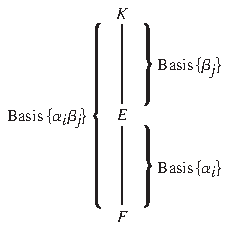
\includegraphics[width=0.310\linewidth,height=.8\textheight,keepaspectratio]{assets/p338_03.pdf}\end{center}
\begin{center}\small\textbf{40.5 Figure}\end{center}
\end{BookFloat}

\begin{center}\begin{adjustbox}{max width=\linewidth}\BookInline{\displaystyle \sum _{i= 1}^{n}c_{ij}\alpha _{i}= 0}\end{adjustbox}\end{center}

\noindent for all \BookInline{j.} But now the \BookInline{\alpha _{i}} are independent over \BookInline{F,\allowbreak } so \BookInline{\sum _{i= 1}^{n}c_{ij}\alpha _{i}= 0} implies that \BookInline{c_{ij}= 0} for all \BookInline{i} and \BookInline{j.} Thus the \BookInline{\alpha _{i}\beta _{j}} not only span \BookInline{K} over \BookInline{F} but also are independent over \BookInline{F.} Thus they form a basis for \BookInline{K} over \BookInline{F.}\BookEnd{\blacklozenge}

Note that we proved this theorem by actually exhibiting a basis. It is worth remembering that if \BookInline{\{\alpha _{i}\mid i= 1,\allowbreak \cdots,\allowbreak n\}} is a basis for \BookInline{E} over \BookInline{F} and \BookInline{\{\beta _{j}\mid j= 1,\allowbreak \cdots,\allowbreak m\}} is a basis for \BookInline{K} over \BookInline{E,\allowbreak } for fields \BookInline{F\leq E\leq K,\allowbreak } then the set \BookInline{\{\alpha _{i}\beta _{j}\}} of \BookInline{mn} products is a basis for \BookInline{K} over \BookInline{F.} Figure 40.5 gives a diagram for this situation. We shall illustrate this further in a moment.

\BookLabel{40.6 Corollary} If \BookInline{F_{i}} is a field for \BookInline{i= 1,\allowbreak \cdots,\allowbreak r} and \BookInline{F_{i+ 1}} is a finite extension of \BookInline{F_{i},\allowbreak } then \BookInline{F_{r}} is a finite extension of \BookInline{F_{1},\allowbreak } and

\begin{center}\begin{adjustbox}{max width=\linewidth}\BookInline{\displaystyle [F_{r}:F_{1}]= [F_{r}:F_{r- 1}][F_{r- 1}:F_{r- 2}]\cdots [F_{2}:F_{1}].}\end{adjustbox}\end{center}

\BookLabel{\textit{Proof}} The proof is a straightforward extension of Theorem 40.4 by induction. \BookEnd{\blacklozenge}

\BookLabel{40.7 Corollary} If \BookInline{E} is an extension field of \BookInline{F,\allowbreak \alpha \in E} is algebraic over \BookInline{F,\allowbreak } and \BookInline{\beta \in F(\alpha ),\allowbreak } then deg\BookInline{(\beta,\allowbreak F)} divides deg\BookInline{(\alpha,\allowbreak F).}

\BookLabel{\textit{Proof}} By Corollary 39.23, deg\BookInline{(\alpha,\allowbreak F)= [F(\alpha ):F]} and deg\BookInline{(\beta,\allowbreak F)= [F(\beta ):F].} We have \BookInline{F\leq } \BookInline{F(\beta )\leq F(\alpha ),\allowbreak } so by Corollary \BookInline{40.6[F(\beta ):F]} divides \BookInline{[F(\alpha ):F].}\BookEnd{\blacklozenge}

The following example illustrates a type of argument one often makes using Theorem 40.4 or its corollaries.

\BookLabel{40.8 Example} By Corollary 40.7, there is no element of \BookInline{\mathbb{Q}(\sqrt{2})} that is a zero of \BookInline{x^{3}- 2.} Note that deg\BookInline{(\sqrt{2},\allowbreak \mathbb{Q})= 2,\allowbreak } while a zero of \BookInline{x^{3}- 2} is of degree 3 over \BookInline{\mathbb{Q},\allowbreak } but 3 does not divide 2. \BookEnd{\blacktriangle}

Let \BookInline{E} be an extension field of a field \BookInline{F,\allowbreak } and let \BookInline{\alpha _{1},\allowbreak \alpha _{2}} be elements of \BookInline{E,\allowbreak } not necessarily algebraic over \BookInline{F.} By definition\BookInline{,\allowbreak F(\alpha _{1})} is the smallest extension field of \BookInline{F} in \BookInline{E} that contains \BookInline{\alpha _{1}.} Similarly\BookInline{,\allowbreak (F(\alpha _{1}))(\alpha _{2})} can be characterized as the smallest extension field of \BookInline{F} in \BookInline{E} containing both \BookInline{\alpha _{1}} and \BookInline{\alpha _{2}.} We could equally have started with \BookInline{\alpha _{2},\allowbreak } so \BookInline{(F(\alpha _{1}))(\alpha _{2})= (F(\alpha _{2}))(\alpha _{1}).} We denote this field by \BookInline{F(\alpha _{1},\allowbreak \alpha _{2}).} Similarly, for \BookInline{\alpha _{i}\in E,\allowbreak F(\alpha _{1},\allowbreak \cdots,\allowbreak \alpha _{n})} is the smallest extension field of \BookInline{F} in \BookInline{E} containing all the \BookInline{\alpha _{i}} for \BookInline{i= 1,\allowbreak \cdots,\allowbreak n.} We obtain the field \BookInline{F(\alpha _{1},\allowbreak \cdots,\allowbreak \alpha _{n})} from the field \BookInline{F} by\textbf{ adjoining to} \BookInline{F} \textbf{the} \textbf{elements} \BookInline{\alpha _{i}} in \BookInline{E.} Exercise 51 of Section 22 shows that, analogous to an intersection of subgroups of a group, an intersection of subfields of a field \BookInline{E} is again a subfield of \BookInline{E.} Thus \BookInline{F(\alpha _{1},\allowbreak \cdots,\allowbreak \alpha _{n})} can be characterized as the intersection of all subfields of \BookInline{E} containing \BookInline{F} and all the \BookInline{\alpha _{i}} for \BookInline{i= 1,\allowbreak \cdots,\allowbreak n.}

\end{BookBody}

% Source PDF page 339; original printed page 322
\BookSource{339}{322}
\BookNarrativetrue

\begin{BookBody}

\BookLabel{40.9 Example} Consider \BookInline{\mathbb{Q}(\sqrt{2}).} Corollary 39.23 shows that \BookInline{\{1,\allowbreak \sqrt{2}\}} is a basis for \BookInline{\mathbb{Q}(\sqrt{2})} over \BookInline{\mathbb{Q}.} Using the technique demonstrated in Example 39.10, we can easily discover that \BookInline{\sqrt{2}+ \sqrt{3}} is a zero of \BookInline{x^{4}- 10x^{2}+ 1.} By the method demonstrated in Example 28.15, we can show that this polynomial is irreducible in \BookInline{\mathbb{Q}[x]}. Thus irr \BookInline{( \sqrt{2} + \sqrt{3},\allowbreak \mathbb{Q} ) = x^4 - 10x^2 + 1}, so \BookInline{[ \mathbb { Q } ( { \sqrt { 2 } } + { \sqrt { 3 } } ): \mathbb { Q } ] = 4.} Thus \BookInline{( { \sqrt { 2 } } + { \sqrt { 3 } } ) \not \in \mathbb { Q } ( { \sqrt { 2 } } )}, so \BookInline{{ \sqrt { 3 } } \notin \mathbb { Q } ( { \sqrt { 2 } } )}. Consequently, \BookInline{\{1,\allowbreak \sqrt{3}\}} is a basis for \BookInline{\mathbb{Q}(\sqrt{2},\allowbreak \sqrt{3})= (\mathbb{Q}(\sqrt{2}))(\sqrt{3})} over \BookInline{\mathbb{Q}(\sqrt{2}).} The proof of Theorem 40.4 (see the comment following the theorem) then shows that \BookInline{\{1,\allowbreak \sqrt{2},\allowbreak \sqrt{3},\allowbreak \sqrt{6}\}} is a basis for \BookInline{\mathbb{Q}(\sqrt{2},\allowbreak \sqrt{3})} over \BookInline{\mathbb{Q}.}\BookEnd{\blacktriangle}

\BookLabel{40.10 Example} Let \BookInline{2^{1/3}} be the real cube root of 2 and \BookInline{2^{1/2}} be the positive square root of 2. Then \BookInline{2^{1/2}\notin \mathbb{Q}(2^{1/3})} because deg\BookInline{(2^{1/2},\allowbreak \mathbb{Q})= 2} and 2 is not a divisor of \BookInline{3= } deg\BookInline{(2^{1/3},\allowbreak \mathbb{Q}).} Thus \BookInline{[\mathbb{Q}(2^{1/3},\allowbreak 2^{1/2}):\mathbb{Q}(2^{1/3})]= 2.} Hence \BookInline{\{1,\allowbreak 2^{1/3},\allowbreak 2^{2/3}\}} is a basis for \BookInline{\mathbb{Q}(2^{1/3})} over \BookInline{\mathbb{Q}} and \BookInline{\{1,\allowbreak 2^{1/2}\}} is a basis for \BookInline{\mathbb{Q}(2^{1/3},\allowbreak 2^{1/2})} over \BookInline{\mathbb{Q}(2^{1/3}).} Furthermore, by Theorem 40.4 (see the comment following the theorem),

\begin{center}\begin{adjustbox}{max width=\linewidth}\BookInline{\displaystyle \{1,\allowbreak 2^{1/2},\allowbreak 2^{1/3},\allowbreak 2^{5/6},\allowbreak 2^{2/3},\allowbreak 2^{7/6}\}}\end{adjustbox}\end{center}

\noindent is a basis for \BookInline{\mathbb{Q}(2^{1/2},\allowbreak 2^{1/3})} over \BookInline{\mathbb{Q}.} Because \BookInline{2^{7/6}= 2(2^{1/6}),\allowbreak } we have \BookInline{2^{1/6}\in \mathbb{Q}(2^{1/2},\allowbreak 2^{1/3}).} Now \BookInline{2^{1/6}} is a zero of \BookInline{x^{6}- 2,\allowbreak } which is irreducible over \BookInline{\mathbb{Q},\allowbreak } by Eisenstein’s criterion, with \BookInline{p= 2.} Thus

\begin{center}\begin{adjustbox}{max width=\linewidth}\BookInline{\displaystyle \mathbb{Q}\leq \mathbb{Q}(2^{1/6})\leq \mathbb{Q}(2^{1/2},\allowbreak 2^{1/3})}\end{adjustbox}\end{center}

\noindent and by Theorem 40.4

\begin{center}\begin{adjustbox}{max width=\linewidth}\BookInline{\displaystyle \begin{aligned}6&= [\mathbb{Q}(2^{1/2},\allowbreak 2^{1/3}):\mathbb{Q}]= [\mathbb{Q}(2^{1/2},\allowbreak 2^{1/3}):\mathbb{Q}(2^{1/6})][\mathbb{Q}(2^{1/6}):\mathbb{Q}] \\ &= [\mathbb{Q}(2^{1/2},\allowbreak 2^{1/3}):\mathbb{Q}(2^{1/6})](6).\end{aligned}}\end{adjustbox}\end{center}

\noindent Therefore, we must have

\begin{center}\begin{adjustbox}{max width=\linewidth}\BookInline{\displaystyle [\mathbb{Q}(2^{1/2},\allowbreak 2^{1/3}):\mathbb{Q}(2^{1/6})]= 1,\allowbreak }\end{adjustbox}\end{center}

\noindent so \BookInline{\mathbb{Q}(2^{1/2},\allowbreak 2^{1/3})= \mathbb{Q}(2^{1/6}),\allowbreak } by the comment preceding Theorem 40.3. \BookEnd{\blacktriangle}

Example 40.10 shows that it is possible for an extension \BookInline{F(\alpha _{1},\allowbreak \cdots,\allowbreak \alpha _{n})} of a field \BookInline{F} to be actually a simple extension, even though \BookInline{n>1.}

Let us characterize extensions of \BookInline{F} of the form \BookInline{F(\alpha _{1},\allowbreak \cdots,\allowbreak \alpha _{n})} in the case that all the \BookInline{\alpha _{i}} are algebraic over \BookInline{F.}

\BookLabel{40.11 Theorem} Let \BookInline{E} be an algebraic extension of a field \BookInline{F.} Then there exist a finite number of elements \BookInline{\alpha _{1},\allowbreak \cdots,\allowbreak \alpha _{n}} in \BookInline{E} such that \BookInline{E= F(\alpha _{1},\allowbreak \cdots,\allowbreak \alpha _{n})} if and only if \BookInline{E} is a finite-dimensional vector space over \BookInline{F,\allowbreak } that is, if and only if \BookInline{E} is a finite extension of \BookInline{F.}

\BookLabel{\textit{Proof}} Suppose that \BookInline{E= F(\alpha _{1},\allowbreak \cdots,\allowbreak \alpha _{n}).} Since \BookInline{E} is an algebraic extension of \BookInline{F,\allowbreak } each \BookInline{\alpha _{i}} is algebraic over \BookInline{F,\allowbreak } so each \BookInline{\alpha _{i}} is algebraic over every extension field of \BookInline{F} in \BookInline{E.} Thus \BookInline{F(\alpha _{1})} is algebraic over \BookInline{F,\allowbreak } and in general\BookInline{,\allowbreak F(\alpha _{1},\allowbreak \cdots,\allowbreak \alpha _{j})} is algebraic over \BookInline{F(\alpha _{i},\allowbreak \cdots,\allowbreak \alpha _{j- 1})} for \BookInline{j= 2,\allowbreak \cdots,\allowbreak n.} Corollary 40.6 applied to the sequence of finite extensions

\begin{center}\begin{adjustbox}{max width=\linewidth}\BookInline{\displaystyle F,\allowbreak F(\alpha _{1}),\allowbreak F(\alpha _{1},\allowbreak \alpha _{2}),\allowbreak \cdots ,\allowbreak F(\alpha _{1},\allowbreak \cdots ,\allowbreak \alpha _{n})= E}\end{adjustbox}\end{center}

\noindent then shows that \BookInline{E} is a finite extension of \BookInline{F.}

Conversely, suppose that \BookInline{E} is a finite algebraic extension of \BookInline{F.} If \BookInline{[E:F]= 1,\allowbreak } then \BookInline{E= F(1)= F,\allowbreak } and we are done. If \BookInline{E\neq F,\allowbreak } let \BookInline{\alpha _{1}\in E,\allowbreak } where \BookInline{\alpha _{1}\notin F.} Then \BookInline{[F(\alpha _{1}):F]>1.} If \BookInline{F(\alpha _{1})= E,\allowbreak } we are done; if not, let \BookInline{\alpha _{2}\in E,\allowbreak } where \BookInline{\alpha _{2}\notin F(\alpha _{1}).} Continuing this process, we see from Theorem 40.4 that since \BookInline{[E:F]} is finite, we must arrive at \BookInline{\alpha _{n}} such that

\begin{center}\begin{adjustbox}{max width=\linewidth}\BookInline{\displaystyle F(\alpha _{1},\allowbreak \cdots ,\allowbreak \alpha _{n})= E.}\end{adjustbox}\end{center} \BookEnd{\blacklozenge}

\end{BookBody}

% Source PDF page 340; original printed page 323
\BookSource{340}{323}
\BookNarrativetrue

\begin{BookBody}

\BookTextHeading{\textbf{Algebraically Closed Fields and Algebraic Closures}  }

\noindent We have not yet observed that if \BookInline{E} is an extension of a field \BookInline{F} and \BookInline{\alpha,\allowbreak \beta \in E} are algebraic over \BookInline{F,\allowbreak } then so are \BookInline{\alpha + \beta,\allowbreak \alpha \beta,\allowbreak \alpha - \beta,\allowbreak } and \BookInline{\alpha /\beta,\allowbreak } if \BookInline{\beta \neq 0.} This follows from Theorem 40.3 and is also included in the following theorem.

\BookLabel{40.12 Theorem} Let \BookInline{E} be an extension field of \BookInline{F.} Then

\begin{center}\begin{adjustbox}{max width=\linewidth}\BookInline{\displaystyle F_{E}= \{\alpha \in E\mid \alpha \;\text{is algebraic over}\;F\}}\end{adjustbox}\end{center}

\noindent is a subfield of \BookInline{E,\allowbreak } the\textbf{ algebraic closure of} \BookInline{F} \textbf{in} \BookInline{E.}

\BookLabel{\textit{Proof}} Let \BookInline{\alpha,\allowbreak \beta \in F_{E}.} Then Theorem 40.11 shows that \BookInline{F(\alpha,\allowbreak \beta )} is a finite extension of \BookInline{F,\allowbreak } and by Theorem 40.3 every element of \BookInline{F(\alpha,\allowbreak \beta )} is algebraic over \BookInline{F,\allowbreak } that is\BookInline{,\allowbreak F(\alpha,\allowbreak \beta )\subseteq F_{E}.} Thus \BookInline{F_{E}} contains \BookInline{\alpha + \beta,\allowbreak \alpha \beta,\allowbreak \alpha - \beta,\allowbreak } and also contains \BookInline{\alpha /\beta } for \BookInline{\beta \neq 0,\allowbreak } so \BookInline{F_{E}} is a subfield of \BookInline{E.} \BookEnd{\blacklozenge}

\BookLabel{40.13 Corollary} The set of all algebraic numbers forms a field.

\BookLabel{\textit{Proof}} Proof of this corollary is immediate from Theorem 40.12, because the set of all algebraic numbers is the algebraic closure of \BookInline{\mathbb{Q}} in \BookInline{\mathbb{C}.}\BookEnd{\blacklozenge}

It is well known that the complex numbers have the property that every nonconstant polynomial in \BookInline{\mathbb{C}[x]} has a zero in \BookInline{\mathbb{C}.} This is known as the\textit{ Fundamental Theorem of} \textit{Algebra}. An analytic proof of this theorem is given in Theorem 40.18. We now give a definition generalizing this important concept to other fields.

\BookLabel{40.14 Definition} A field \BookInline{F} is\textbf{ algebraically closed} if every nonconstant polynomial in \BookInline{F[x]} has a zero in \BookInline{F.}\BookEnd{\blacksquare}

Note that a field \BookInline{F} can be the algebraic closure of \BookInline{F} in an extension field \BookInline{E} without \BookInline{F} being algebraically closed. For example\BookInline{,\allowbreak \mathbb{Q}} is the algebraic closure of \BookInline{\mathbb{Q}} in \BookInline{\mathbb{Q}(x),\allowbreak } but \BookInline{\mathbb{Q}} is not algebraically closed because \BookInline{x^{2}+ 1} has no zero in \BookInline{\mathbb{Q}.}

The next theorem shows that the concept of a field being algebraically closed can also be defined in terms of factorization of polynomials over the field.

\BookLabel{40.15 Theorem} A field \BookInline{F} is algebraically closed if and only if every nonconstant polynomial in \BookInline{F[x]} factors in \BookInline{F[x]} into linear factors.

\BookLabel{\textit{Proof}} Let \BookInline{F} be algebraically closed, and let \BookInline{f(x)} be a nonconstant polynomial in \BookInline{F[x]} Then \BookInline{f(x)} has a zero \BookInline{a\in F.} By Corollary \BookInline{28.4,\allowbreak x- a} is a factor of \BookInline{f(x),\allowbreak } so \BookInline{f(x)= } \BookInline{(x- a)g(x).} Then if \BookInline{g(x)} is nonconstant, it has a zero \BookInline{b\in F,\allowbreak } and we have \BookInline{f(x)= } \BookInline{(x- a)(x- b)h(x).} Continuing, we get a factorization of \BookInline{f(x)} in \BookInline{F[x]} into linear factors. Conversely, suppose that every nonconstant polynomial of \BookInline{F[x]} has a factorization into linear factors. If\textit{ ax} \BookInline{- b} is a linear factor of \BookInline{f(x),\allowbreak } then \BookInline{b/a} is a zero of \BookInline{f(x).} Thus \BookInline{F} is algebraically closed\BookInline{.}\BookEnd{\blacklozenge}

\BookLabel{40.16 Corollary} An algebraically closed field \BookInline{F} has no proper algebraic extensions, that is, no algebraic extensions \BookInline{E} with \BookInline{F<E.}

\BookLabel{\textit{Proof}} Let \BookInline{E} be an algebraic extension of \BookInline{F,\allowbreak } so \BookInline{F\leq E.} Then if \BookInline{\alpha \in E,\allowbreak } we have irr\BookInline{(\alpha,\allowbreak F)= } \BookInline{x- \alpha,\allowbreak } by Theorem 40.15, since \BookInline{F} is algebraically closed. Thus \BookInline{\alpha \in F,\allowbreak } and we must have \BookInline{F= E.}\BookEnd{\blacklozenge}

In a moment we shall show that just as there exists an algebraically closed extension \BookInline{\mathbb{C}} of the real numbers \BookInline{\mathbb{R},\allowbreak } for any field \BookInline{F} there exists similarly an algebraic extension \BookInline{F} of \BookInline{F,\allowbreak } with the property that \BookInline{\overline{F}} is algebraically closed. Naively, to find \BookInline{\overline{F}} we proceed 
% Source PDF page 341; original printed page 324
\BookSource{341}{324}
as follows. If a polynomial \BookInline{f(x)} in \BookInline{F[x]} has no zero in \BookInline{F,\allowbreak } then adjoin a zero \BookInline{\alpha } of such an \BookInline{f(x)} to \BookInline{F,\allowbreak } thus obtaining the field \BookInline{F(\alpha ).} \textit{Theorem 39.3, Kronecker’}\BookInline{s} \textit{theorem, is strongly} \textit{used here, of course}. If \BookInline{F(\alpha )} is still not algebraically closed, then continue the process further. The trouble is that, contrary to the situation for the algebraic closure \BookInline{\mathbb{C}} of \BookInline{\mathbb{R},\allowbreak } we may have to do this a (possibly large) infinite number of times. It can be shown (see Exercises 33 and 36) that \BookInline{\overline{\mathbb{Q}}} is isomorphic to the field of all algebraic numbers, and that we cannot obtain \BookInline{\mathbb{Q}} from \BookInline{\mathbb{Q}} by adjoining a finite number of algebraic numbers. We shall have to first discuss some set-theoretic machinery,\textit{ Zorn’}\BookInline{s} \textit{lemma}, in order to be able to handle such a situation. This machinery is a bit complex, so we are putting the proof under a separate heading. The existence theorem for \BookInline{\overline{F}} is very important, and we state it here so that we will know this fact, even if we do not study the proof.

\end{BookBody}

\BookNarrativetrue

\begin{BookBody}

\BookLabel{40.17 Theorem} Every field \BookInline{F} has an\textbf{ algebraic closure}, that is, an algebraic extension \BookInline{\overline{F}} that is algebraically closed.

The Fundamental Theorem of Algebra stating that \BookInline{\mathbb{C}} is an algebraically closed field is well known. Interestingly, the simplest and shortest proofs of the Fundamental Theorem of Algebra are not algebraic proofs. There are much shorter and easier-to-follow proofs using either analysis or topology. However, behind both the analytical and the topological proofs lies a significant amount of machinery, so perhaps comparing the proofs is not completely fair. At any rate, we include a short proof for students who have studied functions of a complex variable and are familiar with Liouville’s Theorem.

\BookLabel{40.18 Theorem} \textbf{(Fundamental Theorem of Algebra)} The field \BookInline{\mathbb{C}} of complex numbers is an algebraically closed field.

\BookLabel{\textit{Proof}} Let the polynomial \BookInline{f(z)\in \mathbb{C}[z]} have no zero in \BookInline{\mathbb{C}.} Then \BookInline{1/f(z)} gives an entire function; that is\BookInline{,\allowbreak 1/f(z)} is analytic everywhere. Also if \BookInline{f(z)\notin \mathbb{C},\allowbreak } lim \BookInline{\scriptstyle | z | \to \infty | f ( z ) | = \infty} so lim\BookInline{|z|\to \infty } \BookInline{|1/f(z)|= 0.} Thus \BookInline{1/f(z)} must be bounded in the plane. Hence by Liouville’s theorem of complex function theory\BookInline{,\allowbreak 1/f(z)} is constant, and thus \BookInline{f(z)} is constant. Therefore, a nonconstant polynomial in \BookInline{\mathbb{C}[z]} must have a zero in \BookInline{\mathbb{C},\allowbreak } so \BookInline{\mathbb{C}} is algebraically closed. \BookEnd{\blacklozenge}

\BookLabel{\textit{Proof}} \textbf{ of the Existence of an Algebraic Closure}

\noindent We shall prove that every field has an algebraic extension that is algebraically closed. Mathematics students should have the opportunity to see some proof involving the\textit{ Ax}\textit{iom of Choice} by the time they finish college. This is a natural place for such a proof. We shall use an equivalent form,\textit{ Zorn’}\BookInline{s} \textit{lemma}, of the Axiom of Choice. To state Zorn’s lemma, we have to give a set-theoretic definition.

\BookLabel{40.19 Definition} A\textbf{ partial ordering of a set} \BookInline{S} is given by a relation \BookInline{\leq } defined for certain ordered pairs of elements of S such that the following conditions are satisfied:

\BookExercise{1.}{\BookInline{a\leq a} for all \BookInline{a\in S(}\textbf{reflexive law).}}

\BookExercise{2.}{If \BookInline{a\leq b} and \BookInline{b\leq a,\allowbreak } then \BookInline{a= b(}\textbf{antisymmetric law).}}

\BookExercise{3.}{If \BookInline{a\leq b} and \BookInline{b\leq c,\allowbreak } then \BookInline{a\leq c(}\textbf{transitive law).}} \BookEnd{\blacksquare}

In a\textit{ partially} ordered set, not every two elements need be\textbf{ comparable;} that is, for \BookInline{a,\allowbreak b\in S,\allowbreak } we need not have either \BookInline{a\leq b} or \BookInline{b\leq a.} As usual\BookInline{,\allowbreak a<b} denotes \BookInline{a\leq b} but \BookInline{a\neq b.}

A subset \BookInline{T} of a partially ordered set \BookInline{S} is a\textbf{ chain} if every two elements \BookInline{a} and \BookInline{b} in \BookInline{T} are comparable, that is, either \BookInline{a\leq b} or \BookInline{b\leq a(}or both). An element \BookInline{u\in S} is an

\end{BookBody}

% Source PDF page 342; original printed page 325
\BookSource{342}{325}
\BookNarrativetrue

\begin{BookBody}

\noindent \textbf{upper bound for a subset} \BookInline{A} of partially ordered set \BookInline{S} if \BookInline{a\leq u} for all \BookInline{a\in A.} Finally, an element \BookInline{m} of a partially ordered set \BookInline{S} is\textbf{ maximal} if there is no \BookInline{s\in S} such that \BookInline{m<s.}

\BookLabel{40.20 Example} The collection of all subsets of a set forms a partially ordered set under the relation \BookInline{\leq } given by \BookInline{\subseteq.} For example, if the whole set is \BookInline{\mathbb{R},\allowbreak } we have \BookInline{\mathbb{Z}\subseteq \mathbb{Q}.} Note, however, that for \BookInline{\mathbb{Z}} and \BookInline{\mathbb{Q}^{+ },\allowbreak } neither \BookInline{\mathbb{Z}\subseteq \mathbb{Q}^{+ }} nor \BookInline{\mathbb{Q}^{+ }\subseteq \mathbb{Z}.}\BookEnd{\blacktriangle}

\BookExercise{40.}{\textbf{40.21 Zorn’s Lemma}}

\noindent If \BookInline{S} is a partially ordered set such that every chain in \BookInline{S} has an upper bound in \BookInline{S,\allowbreak } then \BookInline{S} has at least one maximal element.

\noindent We do not prove Zorn’s lemma. Instead we point out that it can be shown that Zorn’s lemma is equivalent to the Axiom of Choice. Thus we are really taking Zorn’s lemma here as an\textit{ axiom} for our set theory. Refer to the literature for a statement of the Axiom of Choice and a proof of its equivalence to Zorn’s lemma. (See Edgerton [47].)

Zorn’s lemma is often useful when we want to show the existence of a largest or maximal structure of some kind. If a field \BookInline{F} has an algebraic extension \BookInline{\overline{F}} that is algebraically closed, then \BookInline{\overline{F}} will certainly be a maximal algebraic extension of \BookInline{F,\allowbreak } for since \BookInline{\overline{F}} is algebraically closed, it can have no proper algebraic extensions.

The idea of our proof of Theorem 40.17 is very simple. Given a field \BookInline{F,\allowbreak } we shall first describe a class of algebraic extensions of \BookInline{F} that is so large that it must contain (up to isomorphism) any conceivable algebraic extension of \BookInline{F.} We then define a partial ordering, the ordinary subfield ordering, on this class, and show that the hypotheses of Zorn’s lemma are satisfied. By Zorn’s lemma, there will exist a maximal algebraic extension \BookInline{\overline{F}} of \BookInline{F} in this class. We shall then argue that, as a maximal element, this extension \BookInline{F} can have no proper algebraic extensions, so it must be algebraically closed.

Our proof differs a bit from the one found in many texts. We like it because it uses no algebra other than that derived from Theorems 39.3 and 40.4. Thus it throws into sharp relief the tremendous strength of both Kronecker’s theorem and Zorn’s lemma. The proof looks long, but only because we are writing out every little step. To the professional mathematician, the construction of the proof from the information in the preceding paragraph is a routine matter. This proof was suggested to the author during his graduate student days by a fellow graduate student, Norman Shapiro, who also had a strong preference for it.

We are now ready to carry out our proof of Theorem 40.17, which we restate here.

\BookSubheading{40.22 Restated Theorem 40.17}
Every field \BookInline{F} has an algebraic closure \BookInline{\overline{F}.}

\BookLabel{\textit{Proof}} It can be shown in set theory that given any set, there exists a set with\textit{ strictly more} elements. Suppose we form a set

\begin{center}\begin{adjustbox}{max width=\linewidth}\BookInline{\displaystyle A= \{\omega _{f,\allowbreak i}\mid f\in F[x];i= 0,\allowbreak \cdots ,\allowbreak (\;\text{degree}\;f)\}}\end{adjustbox}\end{center}

\noindent that has an element for every possible zero of any \BookInline{f(x)\in F[x].} Let \BookInline{\Omega } be a set with strictly more elements than \BookInline{A.} Replacing \BookInline{\Omega } by \BookInline{\Omega \cup F} if necessary, we can assume \BookInline{F\subset \Omega.} Consider all possible fields that are algebraic extensions of \BookInline{F} and that, as sets, consist of elements of \BookInline{\Omega.} One such algebraic extension is \BookInline{F} itself. If \BookInline{E} is any extension field of \BookInline{F,\allowbreak } and if \BookInline{\gamma \in E} is a zero \BookInline{f(x)\in F[x]} for \BookInline{\gamma \notin F} and deg\BookInline{(\gamma,\allowbreak F)= n,\allowbreak } then renaming \BookInline{\gamma } by \BookInline{\omega } for \BookInline{\omega \in \Omega } and \BookInline{\omega \notin F,\allowbreak } and renaming elements \BookInline{a_{0}+ a_{1}\gamma + \cdots + a_{n- 1}\gamma ^{n- 1}} of \BookInline{F(\gamma )} by distinct elements of \BookInline{\Omega } as the \BookInline{a_{i}} range over \BookInline{F,\allowbreak } we can consider our renamed \BookInline{F(\gamma )} to be an algebraic extension field \BookInline{F(\omega )} of \BookInline{F,\allowbreak } with \BookInline{F(\omega )\subset \Omega } and \BookInline{f(\omega )= 0.} The set \BookInline{\Omega } has enough elements to form \BookInline{F(\omega ),\allowbreak } since \BookInline{\Omega } has more than enough elements to provide \BookInline{n} different zeros for each element of each degree \BookInline{n} in any subset of \BookInline{F[x].}

All algebraic extension fields \BookInline{E_{j}} of \BookInline{F,\allowbreak } with \BookInline{E_{j}\subseteq \Omega,\allowbreak } form a set

\begin{center}\begin{adjustbox}{max width=\linewidth}\BookInline{\displaystyle S= \{E_{j}\mid j\in J\}}\end{adjustbox}\end{center}

\end{BookBody}

% Source PDF page 343; original printed page 326
\BookSource{343}{326}
\BookNarrativetrue

\begin{BookBody}

\BookTextHeading{\ensuremath{\blacksquare} \textbf{HISTORICAL NOTE}  }

\noindent The Axiom of Choice, although used implicitly in the 1870s and 1880s, was first stated explicitly by Ernst Zermelo in 1904 in connection with his proof of the well-ordering theorem, the result that for any set \BookInline{A,\allowbreak } there exists an order–relation \BookInline{<} such that every nonempty subset \BookInline{B} of \BookInline{A} contains a least element with respect to \BookInline{<.} Zermelo’s Axiom of Choice asserted that, given any set \BookInline{M} and the set \BookInline{S} of all subsets of \BookInline{M,\allowbreak } there always exists a “choice” function, a function \BookInline{f:S\to M} such that \BookInline{f(M^{\prime })\in M^{\prime }} for every \BookInline{M^{\prime }} in \BookInline{S.} Zermelo noted, in fact, that “this logical principle cannot \BookInline{...} be reduced to a still simpler one, but it is applied without hesitation everywhere in mathematical deduction.” A few years later he included this axiom in his collection of axioms for set theory, a collection that was slightly modified in 1930 into what is now called Zermelo–Fraenkel set theory, the axiom system generally used today as a basis of that theory.

Zorn’s lemma was introduced by Max Zorn (1906–1993) in 1935. Although he realized that it was equivalent to the well-ordering theorem (itself equivalent to the Axiom of Choice), he claimed that his lemma was more natural to use in algebra because the well-ordering theorem was somehow a “transcendental” principle. Other mathematicians soon agreed with his reasoning. The lemma appeared in 1939 in the first volume of Nicolas Bourbaki’s\textit{ Ele´ments de Mathe´matique}\BookInline{:Les} \textit{Struc}\textit{tures Fondamentales de} \BookInline{I}\textit{’Analyse}. It was used consistently in that work and quickly became an essential part of the mathematician’s toolbox.

\noindent that is partially ordered under our usual subfield inclusion \BookInline{\leq.} One element of \BookInline{S} is \BookInline{F} itself. The preceding paragraphs shows that if \BookInline{F} is far away from being algebraically closed, there will be many fields \BookInline{E_{j}} in \BookInline{S.}

Let \BookInline{T= \{E_{j_{k}}\}} be a chain in \BookInline{S,\allowbreak } and let \BookInline{W= \cup _{k}E_{j_{k}}}. We now make \BookInline{W} into a field. Let \BookInline{\alpha,\allowbreak \beta \in W.} Then there exist \BookInline{E_{j_{1}},\allowbreak E_{j_{2}}\in S,\allowbreak } with \BookInline{\alpha \in E_{j_{1}}} and \BookInline{\beta \in E_{j_{2}}}. Since \BookInline{T} is a chain, one of the fields \BookInline{E_{j_{1}}} and \BookInline{E_{j_{2}}} is a subfield of the other, say \BookInline{E_{j_{1}}\leq E_{j_{2}}}. Then \BookInline{\alpha,\allowbreak \beta \in E_{j_{2}}}, and we use the field operations of \BookInline{E_{j_{2}}} to\textit{ define} the sum of \BookInline{\alpha } and \BookInline{\beta } in \BookInline{W} as \BookInline{(\alpha + \beta )\in E_{j_{2}}} and, likewise, the product as \BookInline{(\alpha \beta )\in E_{j_{2}}}. These operations are well defined in \BookInline{W;} they are independent of our choice of \BookInline{E_{j_{2}}}, since if \BookInline{\alpha,\allowbreak } \BookInline{\beta \in E_{j_{3}}} also, for \BookInline{E_{j_{3}}} in \BookInline{T,\allowbreak } then one of the fields \BookInline{E_{j_{2}}} and \BookInline{E_{j_{3}}} is a subfield of the other, since \BookInline{T} is a chain. Thus we have operations of addition and multiplication defined on \BookInline{W.}

All the field axioms for \BookInline{W} under these operations now follow from the fact that these operations were defined in terms of addition and multiplication in fields. Thus, for example\BookInline{,\allowbreak 1\in F} serves as multiplicative identity in \BookInline{W,\allowbreak } since for \BookInline{\alpha \in W,\allowbreak \;\text{if}\;1,\allowbreak \alpha \in E_{j_{1}}}, then we have \BookInline{1\alpha = \alpha } in \BookInline{E_{j_{i}},\allowbreak } so \BookInline{1\alpha = \alpha } in \BookInline{W,\allowbreak } by definition of multiplication in \BookInline{W.} As further illustration, to check the distributive laws, let \BookInline{\alpha,\allowbreak \beta,\allowbreak \gamma \in W.} Since \BookInline{T} is a chain, we can find one field in \BookInline{T} containing all three elements \BookInline{\alpha,\allowbreak \beta,\allowbreak } and \BookInline{\gamma,\allowbreak } and in this field the distributive laws for \BookInline{\alpha,\allowbreak \beta,\allowbreak } and \BookInline{\gamma } hold. Thus they hold in \BookInline{W.} Therefore, we can view \BookInline{W} as a field, and by construction, \BookInline{E_{j_{k}}\leq W} for every \BookInline{E_{j_{k}}\in T}.

If we can show that \BookInline{W} is algebraic over \BookInline{F,\allowbreak } then \BookInline{W\in S} will be an upper bound for \BookInline{T.} But if \BookInline{\alpha \in W,\allowbreak } then \BookInline{\alpha \in E_{j_{1}}} for some \BookInline{E_{j_{1}}} in \BookInline{T,\allowbreak } so \BookInline{\alpha } is algebraic over \BookInline{F.} Hence \BookInline{W} is an algebraic extension of \BookInline{F} and is an upper bound for \BookInline{T.}

The hypotheses of Zorn’s lemma are thus fulfilled, so there is a maximal element \BookInline{\overline{F}} of \BookInline{S.} We claim that \BookInline{\overline{F}} is algebraically closed. Let \BookInline{f(x)\in \overline{F}[x],\allowbreak } where \BookInline{f(x)\notin \overline{F}.} Suppose that \BookInline{f(x)} has no zero in \BookInline{\overline{F}.} Since \BookInline{\Omega } has many more elements than \BookInline{F} has, we can take \BookInline{\omega \in \Omega,\allowbreak } where \BookInline{\omega \notin \overline{F},\allowbreak } and form a field \BookInline{\overline{F}(\omega )\subseteq \Omega,\allowbreak } with \BookInline{\omega } a zero of \BookInline{f(x),\allowbreak } as we saw in the first paragraph of this proof. Let \BookInline{\beta } be in \BookInline{\overline{F}(\omega ).} Then by Theorem \BookInline{39.19,\allowbreak \beta } is a zero of a polynomial

\begin{center}\begin{adjustbox}{max width=\linewidth}\BookInline{\displaystyle g(x)= \alpha _{0}+ \alpha _{1}x+ \cdots + \alpha _{n}x^{n}}\end{adjustbox}\end{center}

\end{BookBody}

% Source PDF page 344; original printed page 327
\BookSource{344}{327}
\BookNarrativetrue

\begin{BookBody}

\noindent in \BookInline{\overline{F}[x],\allowbreak } with \BookInline{\alpha _{i}\in \overline{F},\allowbreak } and hence each \BookInline{\alpha _{i}} is algebraic over \BookInline{F.} Then by Theorem 40.11 the field \BookInline{F(\alpha _{0},\allowbreak \cdots,\allowbreak \alpha _{n})} is a finite extension of \BookInline{F,\allowbreak } and since \BookInline{\beta } is algebraic over \BookInline{F(\alpha _{0},\allowbreak \cdots,\allowbreak \alpha _{n}),\allowbreak } we also see that \BookInline{F(\alpha _{0},\allowbreak \cdots,\allowbreak \alpha _{n},\allowbreak \beta )} is a finite extension over \BookInline{F(\alpha _{0},\allowbreak \cdots,\allowbreak \alpha _{n}).} Theorem 40.4 then shows that \BookInline{F(\alpha _{0},\allowbreak \cdots,\allowbreak \alpha _{n},\allowbreak \beta )} is a finite extension of \BookInline{F,\allowbreak } so by Theorem \BookInline{40.3,\allowbreak \beta } is algebraic over \BookInline{F.} Hence \BookInline{\overline{F}(\omega )\in S} and \BookInline{\overline{F}<\overline{F}(\omega ),\allowbreak } which contradicts the choice of \BookInline{F} as maximal in \BookInline{S.} Thus \BookInline{f(x)} must have had a zero in \BookInline{\overline{F},\allowbreak } so \BookInline{\overline{F}} is algebraically closed\BookInline{.}\BookEnd{\blacklozenge}

The mechanics of the preceding proof are routine to the professional mathematician. Since it may be the first proof that we have ever seen using Zorn’s lemma, we wrote the proof out in detail.

\end{BookBody}

\BookNarrativefalse

\begin{BookBody}

\BookExerciseTitle{40}

\BookTextHeading{\textbf{Computations}}

\noindent In Exercises 1 through 13, find the degree and a basis for the given field extension. Be prepared to justify your answers.

\BookExercise{1.}{\BookInline{\mathbb{Q}(\sqrt{2})} over \BookInline{\mathbb{Q}}}

\BookExercise{2.}{\BookInline{\mathbb{Q}(\sqrt{2},\allowbreak \sqrt{3})} over \BookInline{\mathbb{Q}}}

\BookExercise{3.}{\BookInline{\mathbb{Q}(\sqrt{2},\allowbreak \sqrt{3},\allowbreak \sqrt{18})} over \BookInline{\mathbb{Q}}}

\BookExercise{4.}{\BookInline{\mathbb{Q}(\sqrt[3]{2},\allowbreak \sqrt{3})} over \BookInline{\mathbb{Q}}}

\BookExercise{5.}{\BookInline{\mathbb{Q}(\sqrt{2},\allowbreak \sqrt[3]{2})} over \BookInline{\mathbb{Q}}}

\BookExercise{6.}{\BookInline{\mathbb{Q}(\sqrt{2}+ \sqrt{3})} over \BookInline{\mathbb{Q}}}

\BookExercise{7.}{\BookInline{\mathbb{Q}(\sqrt{2}\sqrt{3})} over \BookInline{\mathbb{Q}}}

\BookExercise{8.}{\BookInline{\mathbb{Q}(\sqrt{2},\allowbreak \sqrt[3]{5})} over \BookInline{\mathbb{Q}}}

\BookExercise{9.}{\BookInline{\mathbb{Q}(\sqrt[3]{2},\allowbreak \sqrt[3]{6},\allowbreak \sqrt[3]{24})} over \BookInline{\mathbb{Q}}}

\BookExercise{10.}{\BookInline{\mathbb{Q}(\sqrt{2},\allowbreak \sqrt{6})} over \BookInline{\mathbb{Q}(\sqrt{3})}}

\BookExercise{11.}{\BookInline{\mathbb{Q}(\sqrt{2}+ \sqrt{3})} over \BookInline{\mathbb{Q}(\sqrt{3})}}

\BookExercise{12.}{\BookInline{\mathbb{Q}(\sqrt{2},\allowbreak \sqrt{3})} over \BookInline{\mathbb{Q}(\sqrt{2}+ \sqrt{3})}}

\BookExercise{13.}{\BookInline{\mathbb{Q}(\sqrt{2},\allowbreak \sqrt{6}+ \sqrt{10})} over \BookInline{\mathbb{Q}(\sqrt{3}+ \sqrt{5})}}

\BookTextHeading{\textbf{Concepts}}

\noindent In Exercises 14 through 17, correct the definition of the italicized term without reference to the text, if correction is needed, so that it is in a form acceptable for publication.

\BookExercise{14.}{An\textit{ algebraic extension} of a field \BookInline{F} is a field \BookInline{F(\alpha _{1},\allowbreak \alpha _{2},\allowbreak \cdots,\allowbreak \alpha _{n})} where each \BookInline{\alpha _{i}} is a zero of some polynomial in \BookInline{F[x].}}

\BookExercise{15.}{A\textit{ finite extension} \BookInline{\text{fi}eld} of a field \BookInline{F} is one that can be obtained by adjoining a finite number of elements to \BookInline{F.}}

\BookExercise{16.}{The\textit{ algebraic closure} \BookInline{F_{E}} \textit{of} \BookInline{a\text{fi}eldF} \textit{in an extension} \BookInline{\text{fi}eldE} \textit{of} \BookInline{F} is the field consisting of all elements of \BookInline{E} that are algebraic over \BookInline{F.}}

\BookExercise{17.}{A field \BookInline{F} is\textit{ algebraically closed} if and only if every polynomial has a zero in \BookInline{F.}}

\BookExercise{18.}{Show by an example that for a proper extension field \BookInline{E} of a field \BookInline{F,\allowbreak } the algebraic closure of \BookInline{F} in \BookInline{E} need not be algebraically closed.}

\BookExercise{19.}{Determine whether each of the following is true or false.}

\BookExercise{a.}{If a field \BookInline{E} is a finite extension of a field \BookInline{F,\allowbreak } then \BookInline{E} is a finite field.}

\BookExercise{b.}{Every finite extension of a field is an algebraic extension.}

\BookExercise{c.}{Every algebraic extension of a field is a finite extension.}

\BookExercise{d.}{The top field of a finite tower of finite extensions of fields is a finite extension of the bottom field.}

\BookExercise{e.}{\textbf{e}\BookInline{.\mathbb{Q}} is its own algebraic closure in \BookInline{\mathbb{R},\allowbreak } that is\BookInline{,\allowbreak \mathbb{Q}} is\textbf{ algebraically closed in} \BookInline{\mathbb{R}.}}

\BookExercise{f.}{\textbf{f}\BookInline{.\mathbb{C}} is algebraically closed in \BookInline{\mathbb{C}(x),\allowbreak } where \BookInline{x} is an indeterminate.}

\BookExercise{g.}{\textbf{g}\BookInline{.\mathbb{C}(x)} is algebraically closed, where \BookInline{x} is an indeterminate.}

\BookExercise{h.}{The field \BookInline{\mathbb{C}(x)} has no algebraic closure, since \BookInline{\mathbb{C}} already contains all algebraic numbers.}

\BookExercise{i.}{An algebraically closed field must be of characteristic 0.}

\BookExercise{j.}{If \BookInline{E} is an algebraically closed extension field of \BookInline{F,\allowbreak } then \BookInline{E} is an algebraic extension of \BookInline{F.}}

\end{BookBody}

% Continuation on source PDF page 345, preceding Section 41
\BookNarrativefalse

\begin{BookBody}

\BookLabel{\textit{Proof}} \textbf{ Synopsis}

\BookExercise{20.}{Give a one-sentence synopsis of the proof of Theorem 40.3.}

\BookExercise{21.}{Give a one- or two-sentence synopsis of the proof of Theorem 40.4.}

\BookTextHeading{\textbf{Theory}}

\BookExercise{22.}{Let \BookInline{(a+ } \textit{bi}\BookInline{)\; \in \mathbb{C}} where \BookInline{a,\allowbreak b\in \mathbb{R}} and \BookInline{b\neq 0.} Show that \BookInline{\mathbb{C}= \mathbb{R}(a+ } \textit{bi}).}

\BookExercise{23.}{Show that if \BookInline{E} is a finite extension of a field \BookInline{F} and \BookInline{[E:F]} is a prime number, then \BookInline{E} is a simple extension of \BookInline{F} and, indeed\BookInline{,\allowbreak E= F(\alpha )} for every \BookInline{\alpha \in E} not in \BookInline{F.}}

\BookExercise{24.}{Prove that \BookInline{x^{2}- 3} is irreducible over \BookInline{\mathbb{Q}(\sqrt[3]{2}).}}

\BookExercise{25.}{What degree field extensions can we obtain by successively adjoining to a field \BookInline{F} a square root of an element of \BookInline{F} not a square in \BookInline{F,\allowbreak } then a square root of some nonsquare in this new field, and so on? Argue from this that a zero of \BookInline{x^{14}- 3x^{2}+ 12} over \BookInline{\mathbb{Q}} can never be expressed as a rational function of square roots of rational functions of square roots, and so on, of elements of \BookInline{\mathbb{Q}.}}

\BookExercise{26.}{Let \BookInline{E} be a finite extension field of \BookInline{F.} Let \BookInline{D} be an integral domain such that \BookInline{F\subseteq D\subseteq E.} Show that \BookInline{D} is a field.}

\BookExercise{27.}{Prove in detail that \BookInline{\mathbb{Q}(\sqrt{3}+ \sqrt{7})= \mathbb{Q}(\sqrt{3},\allowbreak \sqrt{7}).}}

\BookExercise{28.}{Generalizing Exercise 27, show that if \BookInline{\sqrt{a}+ \sqrt{b}\neq 0,\allowbreak } then \BookInline{\mathbb{Q}(\sqrt{a}+\sqrt{b})=\mathbb{Q}(\sqrt{a},\allowbreak \sqrt{b})} for all \BookInline{a} and \BookInline{b} in \BookInline{\mathbb{Q}.} [\textit{Hint:} Compute \BookInline{(a- b)/(\sqrt{a}+ \sqrt{b}).]}}

\BookExercise{29.}{Let \BookInline{E} be a finite extension of a field \BookInline{F,\allowbreak } and let \BookInline{p(x)\in F[x]} be irreducible over \BookInline{F} and have degree that is not a divisor of \BookInline{[E:F].} Show that \BookInline{p(x)} has no zeros in \BookInline{E.}}

\BookExercise{30.}{Let \BookInline{E} be an extension field of \BookInline{F.} Let \BookInline{\alpha \in E} be algebraic of odd degree over \BookInline{F.} Show that \BookInline{\alpha ^{2}} is algebraic of odd degree over \BookInline{F,\allowbreak } and \BookInline{F(\alpha )= F(\alpha ^{2}).}}

\BookExercise{31.}{Show that if \BookInline{F,\allowbreak E,\allowbreak } and \BookInline{K} are fields with \BookInline{F\leq E\leq K,\allowbreak } then \BookInline{K} is algebraic over \BookInline{F} if and only if \BookInline{E} is algebraic over \BookInline{F,\allowbreak } and \BookInline{K} is algebraic over \BookInline{E.(}You must\textit{ not} assume the extensions are finite.)}

\BookExercise{32.}{Let \BookInline{E} be an extension field of a field \BookInline{F.} Prove that every \BookInline{\alpha \in E} that is not in the algebraic closure \BookInline{F_{E}} of \BookInline{F} in \BookInline{E} is transcendental over \BookInline{F_{E}.}}

\BookExercise{33.}{Let \BookInline{E} be an algebraically closed extension field of a field \BookInline{F.} Show that the algebraic closure \BookInline{F_{E}} of \BookInline{F} in \BookInline{E} is algebraically closed. (Applying this exercise to \BookInline{\mathbb{C}} and \BookInline{\mathbb{Q},\allowbreak } we see that the field of all algebraic numbers is an algebraically closed field.)}

\BookExercise{34.}{Show that if \BookInline{E} is an algebraic extension of a field \BookInline{F} and contains all zeros in \BookInline{\overline{F}} of every \BookInline{f(x)\in F[x],\allowbreak } then \BookInline{E} is an algebraically closed field.}

\BookExercise{35.}{Show that no finite field of odd characteristic is algebraically closed. (Actually, no finite field of characteristic 2 is algebraically closed either.) [\textit{Hint}: By counting, show that for such a finite field \BookInline{F,\allowbreak } some polynomial \BookInline{x^{2}- a,\allowbreak } for some \BookInline{a\in F,\allowbreak } has no zero in \BookInline{F.} See Exercise 32, Section 39.]}

\BookExercise{36.}{Prove that, as asserted in the text, the algebraic closure of \BookInline{\mathbb{Q}} in \BookInline{\mathbb{C}} is not a finite extension of \BookInline{\mathbb{Q}.}}

\BookExercise{37.}{Argue that every finite extension field of \BookInline{\mathbb{R}} is either \BookInline{\mathbb{R}} itself or is isomorphic to \BookInline{\mathbb{C}.}}

\BookExercise{38.}{Use Zorn’s lemma to show that every proper ideal of a ring \BookInline{R} with unity is contained in some maximal ideal.}

\end{BookBody}
\ifdefined\BookMaster\let\BookFinish\relax\else\def\BookFinish{\end{document}}\fi\BookFinish

\clearpage
% !TeX program = xelatex
\ifdefined\BookMaster\else
\documentclass[11pt,oneside]{article}
% !TeX program = xelatex
\usepackage[b5paper,left=22mm,right=22mm,top=20mm,bottom=22mm,footskip=11mm]{geometry}
\usepackage{fontspec}
\setmainfont{TeX Gyre Termes}
\setsansfont{TeX Gyre Heros}
\usepackage{amsmath,amssymb,mathtools,amsthm}
\renewcommand{\cdots}{\mathinner{\cdotp\cdotp\cdotp}}
\usepackage{graphicx,adjustbox,array,booktabs,longtable,multirow,enumitem,changepage,needspace}
\usepackage[table]{xcolor}
\usepackage{fancyhdr}
\raggedbottom
\interfootnotelinepenalty=10000
\newcommand{\BookFootnote}[2]{\begingroup\renewcommand{\thefootnote}{\fnsymbol{footnote}}\footnote[#1]{#2}\endgroup}
\newcommand{\BookFootnoteMark}[1]{\begingroup\renewcommand{\thefootnote}{\fnsymbol{footnote}}\footnotemark[#1]\endgroup}
\newcommand{\BookFootnoteText}[2]{\begingroup\renewcommand{\thefootnote}{\fnsymbol{footnote}}\footnotetext[#1]{#2}\endgroup}
\newenvironment{BookFloat}[1]{\par\addvspace{.6\baselineskip}\noindent\def\BookFloatID{#1}\begin{minipage}{\linewidth}\phantomsection\label{bookfloat:#1:start}}{\phantomsection\label{bookfloat:\BookFloatID:end}\end{minipage}\par\addvspace{.6\baselineskip}}

\usepackage[unicode,hidelinks]{hyperref}
\pagestyle{fancy}
\fancyhf{}
\newcommand{\BookFooter}{}
\fancyfoot[L]{\parbox[b]{\dimexpr\textwidth-15mm}{\footnotesize\BookFooter}}
\fancyfoot[R]{\footnotesize\thepage}
\renewcommand{\headrulewidth}{0pt}
\renewcommand{\footrulewidth}{0pt}
\setlength{\parindent}{0pt}
\setlength{\parskip}{0.2em}
\setlength{\emergencystretch}{3em}
\setlist{nosep,leftmargin=1.7em,labelsep=.65em}
\newif\ifBookNarrative
\BookNarrativetrue
\newenvironment{BookBody}{\setlength{\parindent}{0pt}}{}
\newcommand{\BookStatement}[1]{\par\addvspace{.6\baselineskip}\noindent #1\enspace\ignorespaces}
\newcommand{\BookLabel}[1]{\par\addvspace{.6\baselineskip}\needspace{3\baselineskip}\noindent\textbf{#1}\quad\ignorespaces}
\newcommand{\BookHeading}[1]{\par\addvspace{\baselineskip}\needspace{4\baselineskip}\noindent{\large\bfseries #1}\par\medskip}
\newcommand{\BookSubheading}[1]{\par\addvspace{.7\baselineskip}\needspace{3\baselineskip}\noindent{\bfseries #1}\par\smallskip}
\newcommand{\BookTextHeading}[1]{\par\addvspace{.7\baselineskip}\needspace{3\baselineskip}\noindent #1\par\smallskip}
\newcommand{\BookSectionTitle}[2]{\par\addvspace{1.2\baselineskip}\needspace{5\baselineskip}\noindent\colorbox{gray!25}{\sffamily\bfseries\small SECTION #1}\quad{\large\bfseries #2}\par\medskip}
\newcommand{\BookExerciseTitle}[1]{\par\addvspace{\baselineskip}\needspace{4\baselineskip}\noindent{\color{gray}\rule{1.5mm}{1.5mm}}\enspace{\large\bfseries Exercises #1}\par\medskip}
\newcommand{\BookBullet}[1]{\begin{list}{\textbullet}{\setlength{\leftmargin}{1.7em}\setlength{\labelwidth}{1em}\setlength{\labelsep}{.7em}\setlength{\topsep}{0pt}\setlength{\parsep}{0pt}\setlength{\itemsep}{0pt}}\item #1\end{list}}
\newcommand{\BookExercise}[2]{\begin{list}{\textbf{#1}}{\setlength{\leftmargin}{2.2em}\setlength{\labelwidth}{1.5em}\setlength{\labelsep}{.7em}\setlength{\topsep}{.15em}\setlength{\parsep}{0pt}\setlength{\itemsep}{0pt}}\item #2\end{list}}
\newcommand{\BookEnd}[1]{\unskip\nobreak\hfill\ensuremath{#1}}
\newcommand{\BookSource}[2]{\phantomsection\label{sourcepage:#1}} % Source-page anchors, retained through reflow.
\usepackage{multicol}
\usepackage{tikz}
\newcommand{\BookPartEntry}[2]{\par\noindent\makebox[17mm][l]{\bfseries Section #1}#2\par}
\newcommand{\BookPartTitle}[3]{\par\bigskip\noindent\begin{tikzpicture}\node[anchor=north west,inner sep=0pt,outer sep=0pt] (bookpart) at (0,0) {\begin{minipage}{\dimexpr\linewidth-.5pt}\hspace*{26mm}\begin{minipage}[t]{\dimexpr\linewidth-26mm}\begin{adjustbox}{max width=\linewidth}{\fontsize{20}{24}\selectfont\bfseries #2}\end{adjustbox}\par\vspace{6mm}\hrule\vspace{6mm}{\sffamily\footnotesize\setlength{\parskip}{.3em}#3}\vspace{3mm}\end{minipage}\end{minipage}};\path[shade,top color=gray!60,bottom color=white] (0,0) rectangle ([xshift=24mm]bookpart.south west);\node[anchor=north,font=\sffamily\bfseries\small] at (12mm,-2mm) {PART};\node[anchor=north,font=\sffamily\bfseries\Huge] at (12mm,-7mm) {#1};\end{tikzpicture}\par\bigskip}
\newsavebox{\BookMathBox}
\makeatletter
\newcommand{\BookInline}[1]{\leavevmode\hskip0pt\relax\begingroup\in@{\begin}{#1}\ifin@\sbox{\BookMathBox}{\(#1\)}\ifdim\wd\BookMathBox>\dimexpr\linewidth-1em\relax\resizebox{\dimexpr\linewidth-1em\relax}{!}{\usebox{\BookMathBox}}\else\(#1\)\fi\else\in@{\left}{#1}\ifin@\sbox{\BookMathBox}{\(#1\)}\ifdim\wd\BookMathBox>\dimexpr\linewidth-1em\relax\resizebox{\dimexpr\linewidth-1em\relax}{!}{\usebox{\BookMathBox}}\else\(#1\)\fi\else\(#1\)\fi\fi\endgroup\hskip0pt\relax}
\makeatother
\DeclareMathOperator{\Aut}{Aut}
\DeclareMathOperator{\End}{End}
\DeclareMathOperator{\Hom}{Hom}
\DeclareMathOperator{\GF}{GF}
\DeclareMathOperator{\irr}{irr}
\DeclareMathOperator{\lt}{lt}
\DeclareMathOperator{\lp}{lp}
\providecommand{\textcircled}[1]{\textnormal{(#1)}}

\begin{document}
\fi
\renewcommand{\BookFooter}{Section 41 Geometric Constructions}
\pdfbookmark[0]{Section 41 Geometric Constructions}{41_geometric_constructions}
\ifdefined\BookMaster\else\setcounter{page}{328}\fi
% Source PDF page 345; original printed page 328
\BookSource{345}{328}
\BookNarrativetrue

\begin{BookBody}

\BookSectionTitle{41}{Geometric Constructions\label{bookfootnote:345:2:ref}\BookFootnote{2}{\label{bookfootnote:345:2:text}This section is used only briefly in Section 48.}}

\noindent In this section we digress briefly to give an application demonstrating the power of Theorem 40.4. For a more detailed study of geometric constructions, you are referred to Courant and Robbins [44, Chapter III].

In Euclid’s\textit{ Elements}, geometry is approached from an axiomatic point of view. The first three axioms state that a line segment can be drawn between any two given points, 
% Source PDF page 346; original printed page 329
\BookSource{346}{329}
a line segment can be extended indefinitely to form a line, and a circle can be drawn centered at any given point with any given radius. A straightedge and a compass are objects that can accomplish the tasks set out in these axioms. A natural question asked by the ancient Greek geometers was exactly which points and configurations can be constructed using only a compass and a straightedge. They found many constructions that are well known today including bisecting angles, bisecting line segments, and trisecting line segments. Trisecting an arbitrary angle eluded mathematicians for well over 2000 years before field theory was developed and it was proven that there are some angles that are impossible to trisect using only a straightedge and compass. We shall discuss the impossibility of trisecting an angle and other classical questions.

\end{BookBody}

\BookNarrativetrue

\begin{BookBody}

\BookTextHeading{\textbf{Constructible Numbers}  }

\noindent Let us imagine that we are given only a single line segment that we shall define to be \textit{one unit} in length. A real number \BookInline{\alpha } is\textbf{ constructible} if we can construct a line segment of length \BookInline{|\alpha |} in a finite number of steps from this given segment of unit length by using a straightedge and a compass.

The rules of the game are pretty strict. We suppose that we are given just two points at the moment, the endpoints of our unit line segment, let us suppose that they correspond to the points (0, 0) and (1, 0) in the Euclidean plane. We are allowed to draw a line only with our straightedge through two points that we have already located. Thus we can start by using the straightedge and drawing the line through (0, 0) and (1, 0). We are allowed to open our compass only to a distance between points we have already found. Let us open our compass to the distance between (0, 0) and (1, 0). We can then place the point of the compass at (1, 0) and draw a circle of radius 1, which passes through the point (2, 0). Thus we now have located a third point, (2, 0). Continuing in this way, we can locate points \BookInline{(3,\allowbreak 0),\allowbreak (4,\allowbreak 0),\allowbreak (- 1,\allowbreak 0),\allowbreak (- 2,\allowbreak 0),\allowbreak } and so on. Now open the compass the distance from (0, 0) to (0, 2), put the point at (1, 0), and draw a circle of radius 2. Do the same with the point at \BookInline{(- 1,\allowbreak 0).} We have now found two new points, where these circles intersect, and we can put our straightedge on them to draw what we think of as the \BookInline{y-}axis. Then opening our compass to the distance from (0, 0) to (1, 0), we draw a circle with center at (0, 0) and locate the point (0, 1) where the circle intersects the \BookInline{y-}axis. Continuing in this fashion, we can locate all points \BookInline{(x,\allowbreak y)} with integer coordinates in any rectangle containing the point (0, 0). Without going into more detail, it can be shown that it is possible, among other things, to erect a perpendicular to a given line at a known point on the line, and find a line passing through a known point and parallel to a given line. Our first result is the following theorem.

\BookLabel{41.1 Theorem} If \BookInline{\alpha } and \BookInline{\beta } are constructible real numbers, then so are \BookInline{\alpha + \beta,\allowbreak \alpha - \beta,\allowbreak \alpha \beta,\allowbreak } and \BookInline{\alpha /\beta,\allowbreak } if \BookInline{\beta \neq 0.}

\BookLabel{\textit{Proof}} We are given that \BookInline{\alpha } and \BookInline{\beta } are constructible, so there are line segments of lengths \BookInline{|\alpha |} and \BookInline{|\beta |} available to us. For \BookInline{\alpha,\allowbreak \beta >0,\allowbreak } extend a line segment of length \BookInline{\alpha } with the straightedge. Start at one end of the original segment of length \BookInline{\alpha,\allowbreak } and lay off on the extension the length \BookInline{\beta } with the compass. This constructs a line segment of length \BookInline{\alpha + \beta;\alpha - \beta } is similiarly constructible (see Fig. 41.2). If \BookInline{\alpha } and \BookInline{\beta } are not both positive, an obvious

\begin{BookFloat}{41_geometric_constructions-p346-6}
\begin{center}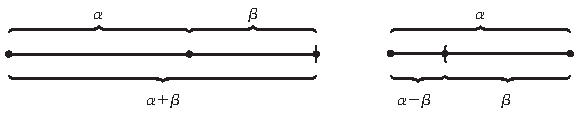
\includegraphics[width=0.793\linewidth,height=.8\textheight,keepaspectratio]{assets/p346_07.pdf}\end{center}
\begin{center}\small\textbf{41.2 Figure}\end{center}
\end{BookFloat}

\end{BookBody}

% Source PDF page 347; original printed page 330
\BookSource{347}{330}
\BookNarrativetrue

\begin{BookBody}

\noindent breakdown into cases according to their signs shows that \BookInline{\alpha + \beta } and \BookInline{\alpha - \beta } are still constructible.

The construction of \BookInline{\alpha \beta } is indicated in Fig. 41.3. We shall let \BookInline{O\overline{A}} be the line segment from the point \BookInline{O} to the point \BookInline{A,\allowbreak } and shall let \BookInline{|OA|} be the length of this line segment. If \BookInline{O\overline{A}} is of length \BookInline{|\alpha |,\allowbreak } construct a line \BookInline{l} through \BookInline{O} not containing \BookInline{O\overline{A}.(}Perhaps, if \BookInline{O} is at (0, 0) and \BookInline{A} is at \BookInline{(a,\allowbreak 0),\allowbreak } you use the line through (0, 0) and (4, 2).) Then find the points \BookInline{P} and \BookInline{B} on \BookInline{l} such that\textit{ OP} is of length 1 and\textit{ OB} is of length \BookInline{|\beta |.} Draw\textit{ PA} and construct \BookInline{l^{\prime }} through \BookInline{B,\allowbreak } parallel to\textit{ PA} and intersecting \BookInline{OA} extended at \BookInline{Q.} By similar triangles, we have

\begin{center}\begin{adjustbox}{max width=\linewidth}\BookInline{\displaystyle { \frac { 1 } { | \alpha | } } = { \frac { | \beta | } { | { \overline { { O Q } } } | } } ,\allowbreak }\end{adjustbox}\end{center}

\noindent so \BookInline{O\overline{Q}} is of length \BookInline{|\alpha \beta |.}

\begin{BookFloat}{41_geometric_constructions-p347-4}
\begin{center}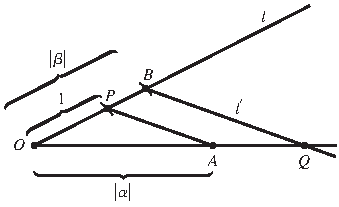
\includegraphics[width=0.466\linewidth,height=.8\textheight,keepaspectratio]{assets/p347_04.pdf}\end{center}
\begin{center}\small\textbf{41.3 Figure}\end{center}
\end{BookFloat}

Finally, Fig. 41.4 shows that \BookInline{\alpha /\beta } is constructible if \BookInline{\beta \neq 0.} Let \BookInline{O\overline{A}} be of length \BookInline{|\alpha |,\allowbreak } and construct \BookInline{l} through \BookInline{O} not containing \BookInline{OA.} Then find \BookInline{B} and \BookInline{P} on \BookInline{l} such that\textit{ OB} is of length \BookInline{|\beta |} and\textit{ OP} is of length 1. Draw \BookInline{BA} and construct \BookInline{l^{\prime }} through \BookInline{P,\allowbreak } parallel to \BookInline{BA,\allowbreak } and intersecting \BookInline{OA} at \BookInline{Q.} Again by similar triangles, we have

\begin{center}\begin{adjustbox}{max width=\linewidth}\BookInline{\displaystyle { \frac { | { \overline { { O Q } } } | } { 1 } } = { \frac { | \alpha | } { | \beta | } } ,\allowbreak }\end{adjustbox}\end{center}

\noindent so \BookInline{O\overline{Q}} is of length \BookInline{|\alpha /\beta |.} \BookEnd{\blacklozenge}

\begin{BookFloat}{41_geometric_constructions-p347-9}
\begin{center}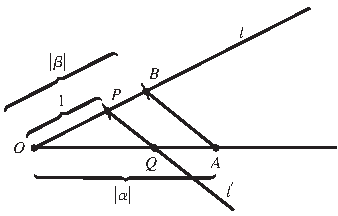
\includegraphics[width=0.464\linewidth,height=.8\textheight,keepaspectratio]{assets/p347_09.pdf}\end{center}
\begin{center}\small\textbf{41.4 Figure}\end{center}
\end{BookFloat}

\BookLabel{41.5 Corollary} The set of all constructible real numbers forms a subfield \BookInline{F} of the field of real numbers.

\BookLabel{\textit{Proof}} Proof of this corollary is immediate from Theorem 41.1. \BookEnd{\blacklozenge}

Thus the field \BookInline{F} of all constructible real numbers contains \BookInline{\mathbb{Q},\allowbreak } the field of rational numbers, since \BookInline{\mathbb{Q}} is the smallest subfield of \BookInline{\mathbb{R}.}

\end{BookBody}

% Source PDF page 348; original printed page 331
\BookSource{348}{331}
\BookNarrativetrue

\begin{BookBody}

From now on, we proceed analytically. We can construct any rational number. Regarding our given segment

0 1

\noindent of length 1 as the basic unit on an \BookInline{x-}axis, we can locate any point \BookInline{(q_{1},\allowbreak q_{2})} in the plane with both coordinates rational. Any further point in the plane that we can locate by using a compass and a straightedge can be found in one of the following three ways:

\BookExercise{1.}{as an intersection of two lines, each of which passes through two known points having rational coordinates,}

\BookExercise{2.}{as an intersection of a line that passes through two points having rational coordinates and a circle whose center has rational coordinates and whose radius is rational.}

\BookExercise{3.}{as an intersection of two circles whose centers have rational coordinates and whose radii are rational.}

Equations of lines and circles of the type discussed in 1, 2, and 3 are of the form

\begin{center}\begin{adjustbox}{max width=\linewidth}\BookInline{\displaystyle ax+ by+ c= 0}\end{adjustbox}\end{center}

\noindent and

\begin{center}\begin{adjustbox}{max width=\linewidth}\BookInline{\displaystyle x^{2}+ y^{2}+ dx+ ey+ f= 0,\allowbreak }\end{adjustbox}\end{center}

\noindent where \BookInline{a,\allowbreak b,\allowbreak c,\allowbreak d,\allowbreak e,\allowbreak } and \BookInline{f} are all in \BookInline{\mathbb{Q}.} Since in Case 3 the intersection of two circles with equations

\begin{center}\begin{adjustbox}{max width=\linewidth}\BookInline{\displaystyle x^{2}+ y^{2}+ d_{1}x+ e_{1}y+ f_{1}= 0}\end{adjustbox}\end{center}

\noindent and

\begin{center}\begin{adjustbox}{max width=\linewidth}\BookInline{\displaystyle x^{2}+ y^{2}+ d_{2}x+ e_{2}y+ f_{2}= 0}\end{adjustbox}\end{center}

\noindent is the same as the intersection of the first circle having equation

\begin{center}\begin{adjustbox}{max width=\linewidth}\BookInline{\displaystyle x^{2}+ y^{2}+ d_{1}x+ e_{1}y+ f_{1}= 0,\allowbreak }\end{adjustbox}\end{center}

\noindent and the line (the common chord) having equation

\begin{center}\begin{adjustbox}{max width=\linewidth}\BookInline{\displaystyle (d_{1}- d_{2})x+ (e_{1}- e_{2})y+ f_{1}- f_{2}= 0,\allowbreak }\end{adjustbox}\end{center}

\noindent we see that Case 3 can be reduced to Case 2. For Case 1, a simultaneous solution of two linear equations with rational coefficients can only lead to rational values of \BookInline{x} and \BookInline{y,\allowbreak } giving us no new points. However, finding a simultaneous solution of a linear equation with rational coefficients and a quadratic equation with rational coefficients, as in Case 2, leads, upon substitution, to a quadratic equation. Such an equation, when solved by the quadratic formula, may have solutions involving square roots of numbers that are not squares in \BookInline{\mathbb{Q}.}

In the preceding argument, nothing was really used involving \BookInline{\mathbb{Q}} except field axioms. If \BookInline{H} is the smallest field containing those real numbers constructed so far, the argument shows that the “next new number” constructed lies in a field \BookInline{H(\sqrt{\alpha })} for some \BookInline{\alpha \in H,\allowbreak } where \BookInline{\alpha >0.} We have proved half of our next theorem.

\BookLabel{41.6 Theorem} The field \BookInline{F} of constructible real numbers consists precisely of all real numbers that we can obtain from \BookInline{\mathbb{Q}} by taking square roots of positive numbers a finite number of times and applying a finite number of field operations.

\BookLabel{\textit{Proof}} We have shown that \BookInline{F} can contain no numbers except those we obtain from \BookInline{\mathbb{Q}} by taking a finite number of square roots of positive numbers and applying a finite number 
% Source PDF page 349; original printed page 332
\BookSource{349}{332}
of field operations. However, if \BookInline{\alpha >0} is constructible, then Fig. 41.7 shows that \BookInline{\sqrt{\alpha }} is constructible. Let \BookInline{O\overline{A}} have length \BookInline{\alpha,\allowbreak } and find \BookInline{P} on \BookInline{O\overline{A}} extended so that\textit{ OP} has length 1. Find the midpoint of\textit{ PA} and draw a semicircle with\textit{ PA} as diameter. Erect a perpendicular to\textit{ PA} at \BookInline{O,\allowbreak } intersecting the semicircle at \BookInline{Q.} Then the triangles \BookInline{OPQ} and \BookInline{OQA} are similar, so

\end{BookBody}

\BookNarrativetrue

\begin{BookBody}

\begin{center}\begin{adjustbox}{max width=\linewidth}\BookInline{\displaystyle \frac { | \overline { { O Q } } | } { | \overline { { O A } } | } = \frac { | \overline { { O P } } | } { | \overline { { O Q } } | } ,\allowbreak }\end{adjustbox}\end{center}

and \BookInline{|O\overline{Q}|^{2}= 1\alpha = \alpha.} Thus \BookInline{O\overline{Q}} is of length \BookInline{\sqrt{\alpha }.} Therefore square roots of constructible numbers are constructible.

Theorem 41.1 showed that field operations are possible by construction\BookInline{.}\BookEnd{\blacklozenge}

\begin{BookFloat}{41_geometric_constructions-p349-4}
\begin{center}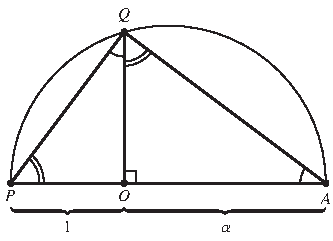
\includegraphics[width=0.457\linewidth,height=.8\textheight,keepaspectratio]{assets/p349_05.pdf}\end{center}
\begin{center}\small\textbf{41.7 Figure}\end{center}
\end{BookFloat}

\BookLabel{41.8 Corollary} If \BookInline{\gamma } is constructible and \BookInline{\gamma \notin \mathbb{Q},\allowbreak } then there is a finite sequence of real numbers \BookInline{\alpha _{1},\allowbreak \cdots,\allowbreak \alpha _{n}= \gamma } such that \BookInline{\mathbb{Q}(\alpha _{1},\allowbreak \cdots,\allowbreak \alpha _{i})} is an extension of \BookInline{\mathbb{Q}(\alpha _{1},\allowbreak \cdots,\allowbreak \alpha _{i- 1})} of degree 2. In particular\BookInline{,\allowbreak [\mathbb{Q}(\gamma ):\mathbb{Q}]= 2^{r}} for some integer \BookInline{r\geq 0.}

\BookLabel{\textit{Proof}} The existence of the \BookInline{\alpha _{i}} is immediate from Theorem 41.6. Then

\begin{center}\begin{adjustbox}{max width=\linewidth}\BookInline{\displaystyle \begin{aligned}2^{n}&= [\mathbb{Q}(\alpha _{1},\allowbreak \cdots ,\allowbreak \alpha _{n}):\mathbb{Q}] \\ &= [\mathbb{Q}(\alpha _{1},\allowbreak \cdots ,\allowbreak \alpha _{n}):\mathbb{Q}(\gamma )][\mathbb{Q}(\gamma ):\mathbb{Q}],\allowbreak \end{aligned}}\end{adjustbox}\end{center}

\noindent by Theorem 40.4, which completes the proof. \BookEnd{\blacklozenge}

\BookTextHeading{\textbf{The Impossibility of Certain Constructions}  }

\noindent We can now show the impossibility of certain geometric constructions.

\BookLabel{41.9 Theorem} \textit{Doubling the cube is impossible,} that is, given a side of a cube, it is not always possible to construct with a straightedge and a compass the side of a cube that has double the volume of the original cube.

\BookLabel{\textit{Proof}} Let the given cube have a side of length 1, and hence a volume of 1. The cube being sought would have to have a volume of 2, and hence a side of length \BookInline{\sqrt { 2 }.} But \BookInline{\sqrt { 2 }} is a zero of irreducible \BookInline{x^{3}- 2} over \BookInline{\mathbb{Q},\allowbreak } so

\begin{center}\begin{adjustbox}{max width=\linewidth}\BookInline{\displaystyle [ \mathbb { Q } ( { \sqrt [ 3 ] { 2 } } ) : \mathbb { Q } ] = 3 .}\end{adjustbox}\end{center}

\noindent Corollary 41.8 shows that to double this cube of volume 1, we would need to have \BookInline{3= 2^{r}} for some integer \BookInline{r,\allowbreak } but no such \BookInline{r} exists\BookInline{.}\BookEnd{\blacklozenge}

\end{BookBody}

% Source PDF page 350; original printed page 333
\BookSource{350}{333}
\BookNarrativetrue

\begin{BookBody}

\BookLabel{41.10 Theorem} \textit{Squaring the circle is impossible;} that is, given a circle, it is not always possible to construct with a straightedge and a compass a square having area equal to the area of the given circle.

\BookLabel{\textit{Proof}} Let the given circle have a radius of 1, and hence an area of \BookInline{\pi.} We would need to construct a square of side \BookInline{\sqrt{\pi }.} But \BookInline{\pi } is transcendental over \BookInline{\mathbb{Q},\allowbreak } so \BookInline{\sqrt{\pi }} is transcendental over \BookInline{\mathbb{Q}} also\BookInline{.}\BookEnd{\blacklozenge}

\BookLabel{41.11 Theorem} \textit{Trisecting the angle is impossible;} that is, there exists an angle that cannot be trisected with a straightedge and a compass.

\BookLabel{\textit{Proof}} Figure 41.12 indicates that the angle \BookInline{\theta } can be constructed if and only if a segment of length \BookInline{|} cos \BookInline{\theta |} can be constructed. Now \BookInline{60^{\circ }} is a constructible angle, and we shall show that it cannot be trisected. Note that

\begin{center}\begin{adjustbox}{max width=\linewidth}\BookInline{\displaystyle \begin{aligned}\;\text{cos}\;3\theta &= \;\text{cos}\;(2\theta + \theta ) \\ &= \;\text{cos}\;2\theta \;\text{cos}\;\theta - \;\text{sin}\;2\theta \;\text{sin}\;\theta  \\ &= (2\;\text{co}\;\mathrm{s}^{2}\theta - 1)\;\text{cos}\;\theta - 2\;\text{sin}\;\theta \;\text{cos}\;\theta \;\text{sin}\;\theta  \\ &= (2\;\text{co}\;\mathrm{s}^{2}\theta - 1)\;\text{cos}\;\theta - 2\;\text{cos}\;\theta (1- \;\text{co}\;\mathrm{s}^{2}\theta ) \\ &= 4\;\text{co}\;\mathrm{s}^{3}\theta - 3\;\text{cos}\;\theta .\end{aligned}}\end{adjustbox}\end{center}

\begin{BookFloat}{41_geometric_constructions-p350-5}
\begin{center}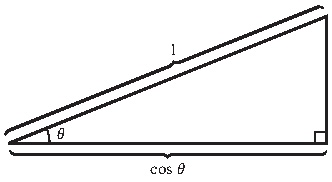
\includegraphics[width=0.455\linewidth,height=.8\textheight,keepaspectratio]{assets/p350_05.pdf}\end{center}
\begin{center}\small\textbf{41.12 Figure}\end{center}
\end{BookFloat}

[We realize that some students have not seen the trigonometric identities we just used. Exercise 1 repeats Exercise 42 of Section 3 and asks you to prove the identity cos \BookInline{3\theta = 4} cos\BookInline{3\theta - 3} cos \BookInline{\theta } from Euler’s formula.]

Let \BookInline{\theta = 20^{\circ },\allowbreak } so that cos \BookInline{3\theta = \frac{1}{2},\allowbreak } and let \BookInline{\alpha = } cos \BookInline{20^{\circ }.} From the identity 4 cos\BookInline{3\theta - } 3 cos \BookInline{\theta = } cos \BookInline{3\theta,\allowbreak } we see that

\begin{center}\begin{adjustbox}{max width=\linewidth}\BookInline{\displaystyle 4\alpha^{3}-3\alpha=\frac{1}{2}.}\end{adjustbox}\end{center}

\noindent Thus \BookInline{\alpha } is a zero of \BookInline{8x^{3}- 6x- 1.} This polynomial is irreducible in \BookInline{\mathbb{Q}[x],\allowbreak } since, by Theorem 28.12, it is enough to show that it does not factor in \BookInline{\mathbb{Z}[x].} But a factorization in \BookInline{\mathbb{Z}[x]} would entail a linear factor of the form \BookInline{(8x\pm 1),\allowbreak (4x\pm 1),\allowbreak (2x\pm 1),\allowbreak } or \BookInline{(x\pm 1).} We can quickly check that none of the numbers \BookInline{\pm \frac{1}{8},\allowbreak \pm \frac{1}{4},\allowbreak \pm \frac{1}{2},\allowbreak } and \BookInline{\pm 1} is a zero of \BookInline{8x^{3}- } \BookInline{6x- 1.} Thus

\begin{center}\begin{adjustbox}{max width=\linewidth}\BookInline{\displaystyle [\mathbb{Q}(\alpha ):\mathbb{Q}]= 3,\allowbreak }\end{adjustbox}\end{center}

\noindent so by Corollary \BookInline{41.8,\allowbreak \alpha } is not constructible. Hence \BookInline{60^{\circ }} cannot be trisected\BookInline{.}\BookEnd{\blacklozenge}

Note that the regular \BookInline{n-}gon is constructible for \BookInline{n\geq 3} if and only if the angle \BookInline{2\pi /n} is constructible, which is the case if and only if a line segment of length cos\BookInline{(2\pi /n)} is constructible.

\end{BookBody}

% Source PDF page 351; original printed page 334
\BookSource{351}{334}
\BookNarrativefalse

\begin{BookBody}

\BookTextHeading{\ensuremath{\blacksquare} \textbf{HISTORICAL NOTE}  }

Greek mathematicians as far back as the fourth century B.C. had tried without success to find geometric constructions using straightedge and compass to trisect the angle, double the cube, and square the circle. Although they were never able to prove that such constructions were impossible, they did manage to construct the solutions to these problems using other tools, including the conic sections.

It was Carl Gauss in the early nineteenth century who made a detailed study of constructibility in connection with his solution of cyclotomic equations, the equations of the form \BookInline{x^{p}- 1= 0} with \BookInline{p} prime whose roots form the vertices of a regular \BookInline{p-}gon. He showed that although all such equations are solvable using radicals, if \BookInline{p- 1} is not a power of 2, then the solutions must involve roots higher than the second. In fact, Gauss asserted that anyone who attempted to find a geometric construction for a \BookInline{p-}gon where \BookInline{p- 1} is not a power of 2 would “spend his time uselessly.” Interestingly, Gauss did not prove the assertion that such constructions were impossible. That was accomplished in 1837 by Pierre Wantzel (1814–1848), who in fact proved Corollary 41.8 and also demonstrated Theorems 41.9 and 41.11. The proof of Theorem 41.10, on the other hand, requires a proof that \BookInline{\pi } is transcendental, a result finally achieved in 1882 by Ferdinand Lindemann (1852–1939).

\BookExerciseTitle{41} \BookEnd{\blacksquare}

\BookTextHeading{\textbf{Computations}}

\BookExercise{1.}{Prove the trigonometric identity cos \BookInline{3\theta = 4} cos\BookInline{3\theta - 3} cos \BookInline{\theta } from the Euler formula\BookInline{,\allowbreak e^{i\theta }= } cos \BookInline{\theta + i} sin \BookInline{\theta.}}

\BookTextHeading{\textbf{Concepts}}

\BookExercise{2.}{Determine whether each of the following is true or false.}

\BookExercise{a.}{It is impossible to double any cube of constructible edge by compass and straightedge constructions.}

\BookExercise{g.}{The fact that factorization of a positive integer into a product of primes is unique (up to order) was used strongly at the conclusion of Theorems 41.9 and 41.11.}

\BookExercise{b.}{It is impossible to double every cube of constructible edge by compass and straightedge constructions.}

\BookExercise{h.}{Counting arguments are exceedingly powerful mathematical tools.}

\BookExercise{c.}{It is impossible to square any circle of constructible radius by straightedge and compass constructions.}

\BookExercise{i.}{We can find any constructible number in a finite number of steps by starting with a given segment of unit length and using a straightedge and a compass.}

\BookExercise{d.}{No constructible angle can be trisected by straightedge and compass constructions.}

\BookExercise{j.}{We can find the totality of all constructible numbers in a finite number of steps by starting with a given segment of unit length and using a straightedge and a compass.}

\BookExercise{e.}{Every constructible number is of degree \BookInline{2^{r}} over \BookInline{\mathbb{Q}} for some integer \BookInline{r\geq 0.}}

\BookExercise{f.}{We have shown that every real number of degree \BookInline{2^{r}} over \BookInline{\mathbb{Q}} for some integer \BookInline{r\geq 0} is constructible.}

\BookTextHeading{\textbf{Theory}}

\BookExercise{3.}{Using the proof of Theorem 41.11, show that the regular 9-gon is not constructible.}

\BookExercise{4.}{Show\textit{ algebraically} that it is possible to construct an angle of \BookInline{30^{\circ }.}}

\end{BookBody}

% Continuation on source PDF page 352, preceding Section 42
\BookNarrativefalse

\begin{BookBody}

\BookExercise{5.}{Referring to Fig. 41.13, where \BookInline{\overline{A}\overline{Q}} bisects angle \BookInline{OAP,\allowbreak } show that the regular 10-gon is constructible (and therefore that the regular pentagon is also). [\textit{Hint:} Triangle \BookInline{OAP} is similar to triangle \BookInline{APQ.} Show algebraically that \BookInline{r} is constructible.]}

\begin{BookFloat}{41_geometric_constructions-p352-1}
\begin{center}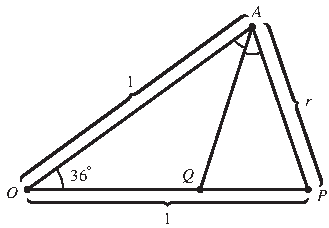
\includegraphics[width=0.452\linewidth,height=.8\textheight,keepaspectratio]{assets/p352_01.pdf}\end{center}
\begin{center}\small\textbf{41.13 Figure}\end{center}
\end{BookFloat}

\noindent In Exercises 6 through 9 use the results of Exercise 5 where needed to show that the statement is true.

\BookExercise{6.}{The regular 20-gon is constructible.}

\BookExercise{7.}{The regular 30-gon is constructible.}

\BookExercise{8.}{The angle \BookInline{72^{\circ }} can be trisected.}

\BookExercise{9.}{The regular 15-gon can be constructed.}

\BookExercise{10.}{Suppose you wanted to explain roughly in just three or four sentences, for a high school plane geometry teacher who never had a course in abstract algebra, how it can be shown that it is impossible to trisect an angle of \BookInline{60^{\circ }.} Write down what you would say.}

\BookExercise{11.}{Let \BookInline{S= \{n\in \mathbb{Z}\mid } an \BookInline{n} degree angle is constructible with a compass and straightedge\BookInline{\}.} We are assuming that if an angle of \BookInline{n} degrees is constructed, then \BookInline{n+ k(360)} is also constructed for any integer \BookInline{k.} Prove that \BookInline{S} is the principal ideal \BookInline{\langle 3\rangle \subseteq \mathbb{Z}.} It may be helpful to use Exercise 5.}

\BookExercise{12.}{The proof of Theorem 41.11 can be simplified by making a different choice of the angle \BookInline{\theta.} Find a constructible real number \BookInline{\alpha } so that the angle \BookInline{\theta = { \frac { \operatorname { a r c c o s } ( \alpha ) } { 3 } }} can be used in the formula cos \BookInline{3\theta = 4} cos\BookInline{3\theta - 3} cos \BookInline{\theta } to arrive at a polynomial that meets Eisenstein’s criteria. Then finish the proof of Theorem 4.11.}

\BookExercise{13.}{Prove that for at least one constructible angle \BookInline{5\theta,\allowbreak \theta } is not constructible.}

\BookExercise{14.}{Continuing Exercise 13,}

\BookExercise{a.}{Use Euler’s formula to show that for any integer \BookInline{n\geq 2,\allowbreak } cos\BookInline{(n\theta )= 2} cos\BookInline{(\theta )} cos\BookInline{((n- 1)\theta )- } cos\BookInline{((n- 2)\theta ).}}

\BookExercise{b.}{Use part a to rewrite cos\BookInline{(7\theta )} and use this formula to prove that there is a constructible angle \BookInline{7\theta } such that \BookInline{\theta } is not constructible.}

\BookExercise{c.}{For each integer \BookInline{1\leq n\leq 10,\allowbreak } is there a constructible angle \BookInline{n\theta } such that \BookInline{\theta } is not constructible?}

(The polynomials used in this exercise are called Chebyshev polynomials.)

\end{BookBody}
\ifdefined\BookMaster\let\BookFinish\relax\else\def\BookFinish{\end{document}}\fi\BookFinish

\clearpage
% !TeX program = xelatex
\ifdefined\BookMaster\else
\documentclass[11pt,oneside]{article}
% !TeX program = xelatex
\usepackage[b5paper,left=22mm,right=22mm,top=20mm,bottom=22mm,footskip=11mm]{geometry}
\usepackage{fontspec}
\setmainfont{TeX Gyre Termes}
\setsansfont{TeX Gyre Heros}
\usepackage{amsmath,amssymb,mathtools,amsthm}
\renewcommand{\cdots}{\mathinner{\cdotp\cdotp\cdotp}}
\usepackage{graphicx,adjustbox,array,booktabs,longtable,multirow,enumitem,changepage,needspace}
\usepackage[table]{xcolor}
\usepackage{fancyhdr}
\raggedbottom
\interfootnotelinepenalty=10000
\newcommand{\BookFootnote}[2]{\begingroup\renewcommand{\thefootnote}{\fnsymbol{footnote}}\footnote[#1]{#2}\endgroup}
\newcommand{\BookFootnoteMark}[1]{\begingroup\renewcommand{\thefootnote}{\fnsymbol{footnote}}\footnotemark[#1]\endgroup}
\newcommand{\BookFootnoteText}[2]{\begingroup\renewcommand{\thefootnote}{\fnsymbol{footnote}}\footnotetext[#1]{#2}\endgroup}
\newenvironment{BookFloat}[1]{\par\addvspace{.6\baselineskip}\noindent\def\BookFloatID{#1}\begin{minipage}{\linewidth}\phantomsection\label{bookfloat:#1:start}}{\phantomsection\label{bookfloat:\BookFloatID:end}\end{minipage}\par\addvspace{.6\baselineskip}}

\usepackage[unicode,hidelinks]{hyperref}
\pagestyle{fancy}
\fancyhf{}
\newcommand{\BookFooter}{}
\fancyfoot[L]{\parbox[b]{\dimexpr\textwidth-15mm}{\footnotesize\BookFooter}}
\fancyfoot[R]{\footnotesize\thepage}
\renewcommand{\headrulewidth}{0pt}
\renewcommand{\footrulewidth}{0pt}
\setlength{\parindent}{0pt}
\setlength{\parskip}{0.2em}
\setlength{\emergencystretch}{3em}
\setlist{nosep,leftmargin=1.7em,labelsep=.65em}
\newif\ifBookNarrative
\BookNarrativetrue
\newenvironment{BookBody}{\setlength{\parindent}{0pt}}{}
\newcommand{\BookStatement}[1]{\par\addvspace{.6\baselineskip}\noindent #1\enspace\ignorespaces}
\newcommand{\BookLabel}[1]{\par\addvspace{.6\baselineskip}\needspace{3\baselineskip}\noindent\textbf{#1}\quad\ignorespaces}
\newcommand{\BookHeading}[1]{\par\addvspace{\baselineskip}\needspace{4\baselineskip}\noindent{\large\bfseries #1}\par\medskip}
\newcommand{\BookSubheading}[1]{\par\addvspace{.7\baselineskip}\needspace{3\baselineskip}\noindent{\bfseries #1}\par\smallskip}
\newcommand{\BookTextHeading}[1]{\par\addvspace{.7\baselineskip}\needspace{3\baselineskip}\noindent #1\par\smallskip}
\newcommand{\BookSectionTitle}[2]{\par\addvspace{1.2\baselineskip}\needspace{5\baselineskip}\noindent\colorbox{gray!25}{\sffamily\bfseries\small SECTION #1}\quad{\large\bfseries #2}\par\medskip}
\newcommand{\BookExerciseTitle}[1]{\par\addvspace{\baselineskip}\needspace{4\baselineskip}\noindent{\color{gray}\rule{1.5mm}{1.5mm}}\enspace{\large\bfseries Exercises #1}\par\medskip}
\newcommand{\BookBullet}[1]{\begin{list}{\textbullet}{\setlength{\leftmargin}{1.7em}\setlength{\labelwidth}{1em}\setlength{\labelsep}{.7em}\setlength{\topsep}{0pt}\setlength{\parsep}{0pt}\setlength{\itemsep}{0pt}}\item #1\end{list}}
\newcommand{\BookExercise}[2]{\begin{list}{\textbf{#1}}{\setlength{\leftmargin}{2.2em}\setlength{\labelwidth}{1.5em}\setlength{\labelsep}{.7em}\setlength{\topsep}{.15em}\setlength{\parsep}{0pt}\setlength{\itemsep}{0pt}}\item #2\end{list}}
\newcommand{\BookEnd}[1]{\unskip\nobreak\hfill\ensuremath{#1}}
\newcommand{\BookSource}[2]{\phantomsection\label{sourcepage:#1}} % Source-page anchors, retained through reflow.
\usepackage{multicol}
\usepackage{tikz}
\newcommand{\BookPartEntry}[2]{\par\noindent\makebox[17mm][l]{\bfseries Section #1}#2\par}
\newcommand{\BookPartTitle}[3]{\par\bigskip\noindent\begin{tikzpicture}\node[anchor=north west,inner sep=0pt,outer sep=0pt] (bookpart) at (0,0) {\begin{minipage}{\dimexpr\linewidth-.5pt}\hspace*{26mm}\begin{minipage}[t]{\dimexpr\linewidth-26mm}\begin{adjustbox}{max width=\linewidth}{\fontsize{20}{24}\selectfont\bfseries #2}\end{adjustbox}\par\vspace{6mm}\hrule\vspace{6mm}{\sffamily\footnotesize\setlength{\parskip}{.3em}#3}\vspace{3mm}\end{minipage}\end{minipage}};\path[shade,top color=gray!60,bottom color=white] (0,0) rectangle ([xshift=24mm]bookpart.south west);\node[anchor=north,font=\sffamily\bfseries\small] at (12mm,-2mm) {PART};\node[anchor=north,font=\sffamily\bfseries\Huge] at (12mm,-7mm) {#1};\end{tikzpicture}\par\bigskip}
\newsavebox{\BookMathBox}
\makeatletter
\newcommand{\BookInline}[1]{\leavevmode\hskip0pt\relax\begingroup\in@{\begin}{#1}\ifin@\sbox{\BookMathBox}{\(#1\)}\ifdim\wd\BookMathBox>\dimexpr\linewidth-1em\relax\resizebox{\dimexpr\linewidth-1em\relax}{!}{\usebox{\BookMathBox}}\else\(#1\)\fi\else\in@{\left}{#1}\ifin@\sbox{\BookMathBox}{\(#1\)}\ifdim\wd\BookMathBox>\dimexpr\linewidth-1em\relax\resizebox{\dimexpr\linewidth-1em\relax}{!}{\usebox{\BookMathBox}}\else\(#1\)\fi\else\(#1\)\fi\fi\endgroup\hskip0pt\relax}
\makeatother
\DeclareMathOperator{\Aut}{Aut}
\DeclareMathOperator{\End}{End}
\DeclareMathOperator{\Hom}{Hom}
\DeclareMathOperator{\GF}{GF}
\DeclareMathOperator{\irr}{irr}
\DeclareMathOperator{\lt}{lt}
\DeclareMathOperator{\lp}{lp}
\providecommand{\textcircled}[1]{\textnormal{(#1)}}

\begin{document}
\fi
\renewcommand{\BookFooter}{Section 42 Finite Fields}
\pdfbookmark[0]{Section 42 Finite Fields}{42_finite_fields}
\ifdefined\BookMaster\else\setcounter{page}{335}\fi
% Source PDF page 352; original printed page 335
\BookSource{352}{335}
\BookNarrativetrue

\begin{BookBody}

\BookSectionTitle{42}{Finite Fields}

\noindent The purpose of this section is to determine the structure of all finite fields. We shall show that for every prime \BookInline{p} and positive integer \BookInline{n,\allowbreak } there is exactly one finite field (up to isomorphism) of order \BookInline{p^{n}.} This field GF\BookInline{(p^{n})} is usually referred to as the\textbf{ Galois field of} \textbf{order} \BookInline{p^{n}.} We shall be using quite a bit of our material on cyclic groups. The proofs are simple and elegant.

\BookTextHeading{\textbf{The Structure of a Finite Field}  }

\noindent We now show that all finite fields must have prime-power order.

\BookLabel{42.1 Theorem} Let \BookInline{E} be a finite extension of degree \BookInline{n} over a finite field \BookInline{F.} If \BookInline{F} has \BookInline{q} elements, then \BookInline{E} has \BookInline{q^{n}} elements.

\end{BookBody}

% Source PDF page 353; original printed page 336
\BookSource{353}{336}
\BookNarrativetrue

\begin{BookBody}

\BookLabel{\textit{Proof}} Let \BookInline{\{\alpha _{1},\allowbreak \cdots,\allowbreak \alpha _{n}\}} be a basis for \BookInline{E} as a vector space over \BookInline{F.} By Exercise 21 of Section 33, every \BookInline{\beta \in E} can be\textit{ uniquely} written in the form

\begin{center}\begin{adjustbox}{max width=\linewidth}\BookInline{\displaystyle \beta = b_{1}\alpha _{1}+ \cdots + b_{n}\alpha _{n}}\end{adjustbox}\end{center}

\noindent for \BookInline{b_{i}\in F.} Since each \BookInline{b_{i}} may be any of the \BookInline{q} elements of \BookInline{F,\allowbreak } the total number of such distinct linear combinations of the \BookInline{\alpha _{i}} is \BookInline{q^{n}.}\BookEnd{\blacklozenge}

\BookLabel{42.2 Corollary} If \BookInline{E} is a finite field of characteristic \BookInline{p,\allowbreak } then \BookInline{E} contains exactly \BookInline{p^{n}} elements for some positive integer \BookInline{n.}

\BookLabel{\textit{Proof}} Every finite field \BookInline{E} is a finite extension of a prime field isomorphic to the field \BookInline{\mathbb{Z}_{p},\allowbreak } where \BookInline{p} is the characteristic of \BookInline{E.} The corollary follows at once from Theorem \BookInline{42.1.}\BookEnd{\blacklozenge}

We now turn to the study of the multiplicative structure of a finite field. The following theorem will show us how any finite field can be formed from the prime subfield.

\BookLabel{42.3 Theorem} Let \BookInline{E} be a field of \BookInline{p^{n}} elements contained in an algebraic closure \BookInline{\overline{\mathbb{Z}_{p}}} of \BookInline{\mathbb{Z}_{p}.} The elements of \BookInline{E} are precisely the zeros in \BookInline{\overline{\mathbb{Z}_{p}}} of the polynomial \BookInline{x^{p^{n}}- x} in \BookInline{\mathbb{Z}_{p}[x].}

\BookLabel{\textit{Proof}} The set \BookInline{E^{\ast }} of nonzero elements of \BookInline{E} forms a multiplicative group of order \BookInline{p^{n}- 1} under the field multiplication. For \BookInline{\alpha \in E^{\ast },\allowbreak } the order of \BookInline{\alpha } in this group divides the order \BookInline{p^{n}- 1} of the group. Thus for \BookInline{\alpha \in E^{\ast },\allowbreak } we have \BookInline{\alpha ^{p^{n}- 1}= 1,\allowbreak \;\text{so}\;\alpha ^{p^{n}}= \alpha.} Therefore, every element in \BookInline{E} is a zero of \BookInline{x^{p^{n}}- x.} Since \BookInline{x^{p^{n}}- x} can have at most \BookInline{p^{n}} zeros, we see that \BookInline{E} contains precisely the zeros of \BookInline{x^{p^{n}}- x} in \BookInline{\mathbb{Z}_{p}.}\BookEnd{\blacklozenge}

\BookLabel{42.4 Definition} An element \BookInline{\alpha } of a field is an \BookInline{n}\textbf{th root of unity} if \BookInline{\alpha ^{n}= 1.} It is a\textbf{ primitive} \BookInline{n}\textbf{th root of} \textbf{unity} if \BookInline{\alpha ^{n}= 1} and \BookInline{\alpha ^ { m } \neq 1} for \BookInline{0<m<n.}\BookEnd{\blacksquare}

Thus the nonzero elements of a finite field of \BookInline{p^{n}} elements are all \BookInline{(p^{n}- 1)}th roots of unity.

Recall that in Corollary 28.7, we showed that the multiplicative group of nonzero elements of a finite field is cyclic. This is a very important fact about finite fields; it has actually been applied to coding theory and combinatorics. For the sake of completeness in this section, we now state it here as a theorem, give a corollary, and illustrate with an example.

\BookLabel{42.5 Theorem} The multiplicative group \BookInline{\langle F^{\ast },\allowbreak \cdot \rangle } of nonzero elements of a finite field \BookInline{F} is cyclic.

\BookLabel{\textit{Proof}} See Corollary 28.7. \BookEnd{\blacklozenge}

\BookLabel{42.6 Corollary} A finite extension \BookInline{E} of a finite field \BookInline{F} is a simple extension of \BookInline{F.}

\BookLabel{\textit{Proof}} Let \BookInline{\alpha } be a generator for the cyclic group \BookInline{E^{\ast }} of nonzero elements of \BookInline{E.} Then \BookInline{E= F(\alpha ).} \BookEnd{\blacklozenge}

\BookLabel{42.7 Example} Consider the finite field \BookInline{\mathbb{Z}_{11}.} By Theorem \BookInline{42.5\langle \mathbb{Z}_{11}^{\ast },\allowbreak \cdot \rangle } is cyclic. Let us try to find a generator of \BookInline{\mathbb{Z}_{11}^{\ast }} by brute force and ignorance. We start by trying 2. Since \BookInline{|\mathbb{Z}_{11}^{\ast }|= 10,\allowbreak 2} must be an element of \BookInline{\mathbb{Z}_{11}^{\ast }} of order dividing 10, that is, either 2, 5, or 10. Now

\begin{center}\begin{adjustbox}{max width=\linewidth}\BookInline{\displaystyle 2^{2}= 4,\allowbreak 2^{4}= 4^{2}= 5,\allowbreak \;\text{and}\;2^{5}= (2)(5)= 10= - 1.}\end{adjustbox}\end{center}

\noindent Thus neither 22 nor 25 is 1, but, of course\BookInline{,\allowbreak 2^{10}= 1,\allowbreak } so 2 is a generator of \BookInline{\mathbb{Z}_{11}^{\ast },\allowbreak } that is, 2 is a primitive 10th root of unity in \BookInline{\mathbb{Z}_{11}.} We were lucky.

By the theory of cyclic groups, all the generators of \BookInline{Z_{11}^{\ast },\allowbreak } that is, all the primitive 10th roots of unity in \BookInline{\mathbb{Z}_{11},\allowbreak } are of the form \BookInline{2^{n},\allowbreak } where \BookInline{n} is relatively prime to 10. These elements are

\begin{center}\begin{adjustbox}{max width=\linewidth}\BookInline{\displaystyle 2^{1}= 2,\allowbreak 2^{3}= 8,\allowbreak 2^{7}= 7,\allowbreak 2^{9}= 6.}\end{adjustbox}\end{center}

\end{BookBody}

% Source PDF page 354; original printed page 337
\BookSource{354}{337}
\BookNarrativetrue

\begin{BookBody}

\BookTextHeading{\textbf{HISTORICAL NOTE}  } \BookEnd{\blacksquare}

\noindent Although Carl F. Gauss had shown that the set of residues modulo a prime \BookInline{p} satisfied the field properties, it was Evariste Galois (1811– 1832) who first dealt with what he called “incommensurable solutions” to the congruence \BookInline{F(x)\equiv 0} (mod \BookInline{p),\allowbreak } where \BookInline{F(x)} is an \BookInline{n}th degree irreducible polynomial modulo \BookInline{p.} He noted in a paper written in 1830 that one should consider the roots of this congruence as “a variety of imaginary symbols” that one can use in calculations just as one uses \BookInline{\sqrt{- }1.} Galois then showed that if \BookInline{\alpha } is any solution of \BookInline{F(x)\equiv 0(}mod \BookInline{p),\allowbreak } the expression \BookInline{a_{0}+ a_{1}\alpha + } \BookInline{a_{2}\alpha ^{2}+ \cdots + a_{n- 1}\alpha ^{n- 1}} takes on precisely \BookInline{p^{n}} different values. Finally, he proved results equivalent to Theorems 42.3 and 42.5 of the text.

\noindent Galois’ life was brief and tragic. He showed brilliance in mathematics early on, publishing several papers before he was 20 and essentially established the basic ideas of Galois theory. He was, however, active in French revolutionary politics following the July revolution of 1830. In May 1831, he was arrested for threatening the life of King Louis-Philippe. Though he was acquitted, he was rearrested for participating, heavily armed, in a republican demonstration on Bastille Day of that year. Two months after his release from prison the following March, he was killed in a duel, “the victim of an infamous coquette and her two dupes”; the previous night he had written a letter to a friend clarifying some of his work in the theory of equations and requesting that it be studied by other mathematicians. Not until 1846, however, were his major papers published; it is from that date that his work became influential.

\noindent The primitive 5th roots of unity in \BookInline{\mathbb{Z}_{11}} are of the form \BookInline{2^{m},\allowbreak } where the gcd of \BookInline{m} and 10 is 2, that is,

\begin{center}\begin{adjustbox}{max width=\linewidth}\BookInline{\displaystyle 2^{2}= 4,\allowbreak 2^{4}= 5,\allowbreak 2^{6}= 9,\allowbreak 2^{8}= 3.}\end{adjustbox}\end{center}

\noindent The primitive square root of unity in \BookInline{\mathbb{Z}_{11}} is \BookInline{2^{5}= 10= - 1.} \BookEnd{\blacktriangle}

\noindent \textbf{The Existence of GF}\BookInline{(p^{n})}

\noindent We turn now to the question of the existence of a finite field of order \BookInline{p^{r}} for every prime power \BookInline{p^{r},\allowbreak r>0.} We need the following lemma.

\BookLabel{42.8 Lemma} If \BookInline{F} is a field of prime characteristic \BookInline{p} with algebraic closure \BookInline{\overline{F},\allowbreak } then \BookInline{x^{p^{n}}- x} has \BookInline{p^{n}} distinct zeros in \BookInline{\overline{F}.}

\BookLabel{\textit{Proof}} Because \BookInline{\overline{F}} is algebraically closed, \BookInline{x^{p^{n}}- x} factors over that field into a product of linear factors \BookInline{x- \alpha,\allowbreak } so it suffices to show that none of these factors occurs more than once in the factorization.

Exercise 15 uses derivatives to complete this proof. Although this is an elegant method, it requires some effort to develop derivatives for polynomials over an arbitrary field, so we proceed using long division. Observe that 0 is a zero of \BookInline{x^{p^{n}}- x} of multiplicity 1. Suppose \BookInline{\alpha \neq 0} is a zero of \BookInline{x^{p^{n}}- x,\allowbreak } and hence is a zero of \BookInline{f(x)= x^{p^{n}- 1}- 1}. Then \BookInline{x- \alpha } is a factor of \BookInline{f(x)} in \BookInline{\overline{F}[x],\allowbreak } and by long division, we find that

\begin{center}\begin{adjustbox}{max width=\linewidth}\BookInline{\displaystyle \begin{aligned}\frac{f(x)}{(x - \alpha)} &= g(x) \\= x^{p^{n} - 2} + \alpha x^{p^{n} - 3} + \alpha^{2}x^{p^{n} - 4} &+ \cdots + \alpha^{p^{n} - 3}x + \alpha^{p^{n} - 2}.\end{aligned}}\end{adjustbox}\end{center}

\noindent Now \BookInline{g(x)} has \BookInline{p^{n}- 1} summands, and in \BookInline{g(\alpha ),\allowbreak } each summand is

\begin{center}\begin{adjustbox}{max width=\linewidth}\BookInline{\displaystyle \alpha ^ { p ^ { n } - 2 } = \frac { \alpha ^ { p ^ { n } - 1 } } { \alpha } = \frac { 1 } { \alpha } .}\end{adjustbox}\end{center}

\end{BookBody}

% Source PDF page 355; original printed page 338
\BookSource{355}{338}
\BookNarrativetrue

\begin{BookBody}

\noindent Thus

\begin{center}\begin{adjustbox}{max width=\linewidth}\BookInline{\displaystyle g(\alpha) = [(p^n - 1) \cdot 1] \frac{1}{\alpha} = - \frac{1}{\alpha}.}\end{adjustbox}\end{center}

\noindent since we are in a field of characteristic \BookInline{p.} Therefore\BookInline{,\allowbreak g(\alpha )\neq 0,\allowbreak } so \BookInline{\alpha } is a zero of \BookInline{f(x)} of multiplicity \BookInline{1.}\BookEnd{\blacklozenge}

\BookLabel{42.9 Lemma} If \BookInline{F} is a field of prime characteristic \BookInline{p,\allowbreak } then \BookInline{(\alpha + \beta )^{p^{n}}= \alpha ^{p^{n}}+ \beta ^{p^{n}}} for all \BookInline{\alpha,\allowbreak \beta \in F} and all positive integers \BookInline{n.}

\BookLabel{\textit{Proof}} Let \BookInline{\alpha,\allowbreak \beta \in F.} Applying the binomial theorem to \BookInline{(\alpha + \beta )^{p},\allowbreak } we have

\begin{center}\begin{adjustbox}{max width=\linewidth}\BookInline{\displaystyle \begin{aligned}(\alpha + \beta)^p &= \alpha^p + (p \cdot 1)\alpha^{p-1}\beta + \bigg(\frac{p(p-1)}{2} \cdot 1\bigg)\alpha^{p-2}\beta^2 \\&\quad + \cdots + (p \cdot 1)\alpha\beta^{p-1} + \beta^p \\&= \alpha^p + 0\alpha^{p-1}\beta + 0\alpha^{p-2}\beta^2 + \cdots + 0\alpha\beta^{p-1} + \beta^p \\&= \alpha^p + \beta^p.\end{aligned}}\end{adjustbox}\end{center}

\noindent Proceeding by induction on \BookInline{n,\allowbreak } suppose that we have \BookInline{(\alpha + \beta )^{p^{n- 1}}= \alpha ^{p^{n- 1}}+ \beta ^{p^{n- 1}}}. Then \BookInline{(\alpha + \beta )^{p^{n}}= [(\alpha + \beta )^{p^{n- 1}}]^{p}= (\alpha ^{p^{n- 1}}+ \beta ^{p^{n- 1}})^{p}= \alpha ^{p^{n}}+ \beta ^{p^{n}}.} \BookEnd{\blacklozenge}

\BookLabel{42.10 Theorem} A finite field GF\BookInline{(p^{n})} of \BookInline{p^{n}} elements exists for every prime power \BookInline{p^{n}.}

\BookLabel{\textit{Proof}} Let \BookInline{\overline{\mathbb{Z}_{p}}} be an algebraic closure of \BookInline{\mathbb{Z}_{p},\allowbreak } and let \BookInline{K} be the subset of \BookInline{\overline{\mathbb{Z}_{p}}} consisting of all zeros of \BookInline{x^{p^{n}}- x} in \BookInline{\overline{\mathbb{Z}_{p}}.} Let \BookInline{\alpha,\allowbreak \beta \in K.} Lemma 42.9 shows that \BookInline{(\alpha + \beta )\in K,\allowbreak } and the equation \BookInline{(\alpha \beta )^{p^{n}}= \alpha ^{p^{n}}\beta ^{p^{n}}= \alpha \beta } shows that \BookInline{\alpha \beta \in K.} From \BookInline{\alpha ^{p^{n}}= \alpha } we obtain \BookInline{(- \alpha )^{p^{n}}= } \BookInline{(- 1)^{p^{n}}\alpha ^{p^{n}}= (- 1)^{p^{n}}\alpha.\;\text{If}\;p} is an odd prime, then \BookInline{(- 1)^{p^{n}}= - 1} and if \BookInline{p= 2} then \BookInline{- 1= 1.} Thus \BookInline{(- \alpha )^{p^{n}}= - \alpha,\allowbreak \;\text{so}\;- \alpha \in K}. Now 0 and 1 are zeros of \BookInline{x^{p^{n}}- x.} For \BookInline{\alpha } \BookInline{\neq 0,\allowbreak \alpha ^{p^{n}}= \alpha } implies that \BookInline{(1/\alpha )^{p^{n}}= 1/\alpha }. Thus \BookInline{K} is a subfield of \BookInline{\overline{\mathbb{Z}_{p}}} containing \BookInline{\mathbb{Z}_{p}.} Therefore\BookInline{,\allowbreak K} is the desired field of \BookInline{p^{n}} elements, since Lemma 42.8 showed that \BookInline{x^{p^{n}}- x} has \BookInline{p^{n}} distinct zeros in \BookInline{\overline{\mathbb{Z}_{p}}.}\BookEnd{\blacklozenge}

\BookLabel{42.11 Corollary} If \BookInline{F} is any finite field, then for every positive integer \BookInline{n,\allowbreak } there is an irreducible polynomial in \BookInline{F[x]} of degree \BookInline{n.}

\BookLabel{\textit{Proof}} Let \BookInline{F} have \BookInline{q= p^{r}} elements, where \BookInline{p} is the characteristic of \BookInline{F.} By Theorem 42.10, there is a field \BookInline{K\leq \overline{F}} containing \BookInline{\mathbb{Z}_{p}(}up to isomorphism) and consisting precisely of the zeros of \BookInline{x^{p^{rn}}- x.} We want to show \BookInline{F\leq K.} Every element of \BookInline{F} is a zero of \BookInline{x^{p^{r}}- x,\allowbreak } by Theorem 42.3. Now \BookInline{p^{rs}= p^{r}p^{r(s- 1)}.} Applying this equation repeatedly to the exponents and using the fact that for \BookInline{\alpha \in F} we have \BookInline{\alpha ^{p^{r}}= \alpha }, we see that for \BookInline{\alpha \in F,\allowbreak }

\begin{center}\begin{adjustbox}{max width=\linewidth}\BookInline{\displaystyle \alpha ^{p^{rn}}= \alpha ^{p^{r(n- 1)}}= \alpha ^{p^{r(n- 2)}}= \cdots = \alpha ^{p^{r}}= \alpha .}\end{adjustbox}\end{center}

\noindent Thus \BookInline{F\leq K.} Then Theorem 42.1 shows that we must have \BookInline{[K:F]= n.} We have seen that \BookInline{K} is simple over \BookInline{F} in Corollary 42.6, so \BookInline{K= F(\beta )} for some \BookInline{\beta \in K.} Therefore, irr\BookInline{(\beta,\allowbreak F)} must be of degree \BookInline{n.}\BookEnd{\blacklozenge}

\BookLabel{42.12 Theorem} Let \BookInline{p} be a prime and let \BookInline{n\in \mathbb{Z}^{+ }.} If \BookInline{E} and \BookInline{E^{\prime }} are fields of order \BookInline{p^{n},\allowbreak } then \BookInline{E\simeq E^{\prime }.}

\BookLabel{\textit{Proof}} Both \BookInline{E} and \BookInline{E^{\prime }} have \BookInline{\mathbb{Z}_{p}} as prime field, up to isomorphism. By Corollary \BookInline{42.6,\allowbreak E} is a simple extension of \BookInline{\mathbb{Z}_{p}} of degree \BookInline{n,\allowbreak } so there exists an irreducible polynomial \BookInline{f(x)} of degree \BookInline{n} in \BookInline{\mathbb{Z}_{p}[x]} such that \BookInline{E\simeq \mathbb{Z}_{p}[x]/\langle f(x)\rangle.} Because the elements of \BookInline{E} are zeros of \BookInline{x^{p^{n}}- x,\allowbreak } we see that \BookInline{f(x)} is a factor of \BookInline{x^{p^{n}}- x} in \BookInline{\mathbb{Z}_{p}[x].} Because \BookInline{E^{\prime }} also consists of 
% Source PDF page 356; original printed page 339
\BookSource{356}{339}
zeros of \BookInline{x^{p^{n}}- x,\allowbreak } we see that \BookInline{E^{\prime }} also contains zeros of irreducible \BookInline{f(x)} in \BookInline{\mathbb{Z}_{p}[x].} Thus, because \BookInline{E^{\prime }} also contains exactly \BookInline{p^{n}} elements\BookInline{,\allowbreak E^{\prime }} is also isomorphic to \BookInline{\mathbb{Z}_{p}[x]/\langle f(x)\rangle.}\BookEnd{\blacklozenge}

\end{BookBody}

\BookNarrativetrue

\begin{BookBody}

In section 29 we saw that the field \BookInline{\mathbb{Z}_{2}} can be used to construct polynomial codes. Other finite fields have been used to construct algebraic codes with interesting properties. For example, in the\textit{ American Mathematical Monthly} 77 (1970): 249–258, Normal Levinson constructed an algebraic code that corrects three transmission errors. In this construction, the field of order 16 was used. Finite fields are also used in many other areas of mathematics including combinatorial designs, finite geometries, and algebraic topology.

\end{BookBody}

\BookNarrativefalse

\begin{BookBody}

\BookExerciseTitle{42} \BookEnd{\blacksquare}

\BookTextHeading{\textbf{Computations}}

\noindent In Exercises 1 through 3, determine whether there exists a finite field having the given number of elements. (A calculator may be useful.)

\BookExercise{1.}{4096}

\BookExercise{2.}{3127}

\BookExercise{3.}{68,921}

\BookExercise{4.}{Find the number of primitive 8th roots of unity in GF(9).}

\BookExercise{5.}{Find the number of primitive 18th roots of unity in GF(19).}

\BookExercise{6.}{Find the number of primitive 15th roots of unity in GF(31).}

\BookExercise{7.}{Find the number of primitive 10th roots of unity in GF(23).}

\BookTextHeading{\textbf{Concepts}}

\BookExercise{8.}{Determine whether each of the following is true or false.}

\BookExercise{a.}{The nonzero elements of every finite field form a cyclic group under multiplication.}

\BookExercise{b.}{The elements of every finite field form a cyclic group under addition.}

\BookExercise{c.}{The zeros in \BookInline{\mathbb{C}} of \BookInline{(x^{28}- 1)\in \mathbb{Q}[x]} form a cyclic group under multiplication.}

\BookExercise{d.}{There exists a finite field of 60 elements.}

\BookExercise{e.}{There exists a finite field of 125 elements.}

\BookExercise{f.}{There exists a finite field of 36 elements.}

\BookExercise{g.}{The complex number \BookInline{i} is a primitive 4th root of unity.}

\BookExercise{h.}{There exists an irreducible polynomial of degree 58 in \BookInline{\mathbb{Z}_{2}[x].}}

\BookExercise{i.}{The nonzero elements of \BookInline{\mathbb{Q}} form a cyclic group \BookInline{\mathbb{Q}^{\ast }} under field multiplication.}

\BookExercise{j.}{If \BookInline{F} is a finite field, then every isomorphism mapping \BookInline{F} onto a subfield of an algebraic closure \BookInline{\overline{F}} of \BookInline{F} is an automorphism of \BookInline{F.}}

\BookTextHeading{\textbf{Theory}}

\BookExercise{9.}{Let \BookInline{\overline{\mathbb{Z}_{2}}} be an algebraic closure of \BookInline{\mathbb{Z}_{2},\allowbreak } and let \BookInline{\alpha,\allowbreak \beta \in \overline{\mathbb{Z}_{2}}} be zeros of \BookInline{x^{3}+ x^{2}+ 1} and of \BookInline{x^{3}+ x+ 1,\allowbreak } respectively. Using the results of this section, show that \BookInline{\mathbb{Z}_{2}(\alpha )= \mathbb{Z}_{2}(\beta ).}}

\BookExercise{10.}{Show that every irreducible polynomial in \BookInline{\mathbb{Z}_{p}[x]} is a divisor of \BookInline{x^{p^{n}}- x} for some \BookInline{n.}}

\BookExercise{11.}{Let \BookInline{F} be a finite field of \BookInline{p^{n}} elements containing the prime subfield \BookInline{\mathbb{Z}_{p}.} Show that if \BookInline{\alpha \in F} is a generator of the cyclic group \BookInline{\langle F^{\ast },\allowbreak \cdot \rangle } of nonzero elements of \BookInline{F,\allowbreak } then deg\BookInline{(\alpha,\allowbreak \mathbb{Z}_{p})= n.}}

\BookExercise{12.}{Show that a finite field of \BookInline{p^{n}} elements has exactly one subfield of \BookInline{p^{m}} elements for each divisor \BookInline{m} of \BookInline{n.}}

\BookExercise{13.}{Show that \BookInline{x^{p^{n}}- x} is the product of all monic irreducible polynomials in \BookInline{\mathbb{Z}_{p}[x]} of a degree \BookInline{d} dividing \BookInline{n.}}

\BookExercise{14.}{Let \BookInline{p} be an odd prime.}

\end{BookBody}

% Source PDF page 357; original printed page 340
\BookSource{357}{340}
\BookNarrativefalse

\begin{BookBody}

\BookExercise{a.}{Show that for \BookInline{a\in \mathbb{Z},\allowbreak } where \BookInline{a\not \equiv 0(}mod \BookInline{p),\allowbreak } the congruence \BookInline{x^{2}\equiv a(}mod \BookInline{p)} has a solution in \BookInline{\mathbb{Z}} if and only if \BookInline{a^{(p- 1)/2}\equiv 1(}mod \BookInline{p).[}\textit{Hint:} Formulate an equivalent statement in the finite field \BookInline{\mathbb{Z}_{p},\allowbreak } and use the theory of cyclic groups.]}

\BookExercise{b.}{Using part (a), determine whether or not the polynomial \BookInline{x^{2}- 6} is irreducible in \BookInline{\mathbb{Z}_{17}[x].}}

\BookInline{f p ( x ) = \sum _ { k = 0 } ^ { n } a _ { k } x ^ { k } \in F [ x ] \operatorname { t o } \operatorname { b e } D ( p ( x ) ) = \sum _ { k = 1 } ^ { n } \left( k \cdot ( a _ { k } x ^ { k - 1 } ) \right)}

\BookExercise{15.}{Let \BookInline{F} be an arbitrary field. We define the\textbf{ derivative} of \BookInline{p(x)= \sum _{k= 0}a_{k}x^{k}\in F[x]\;\text{to be}\;D(p(x))= \sum _{k= 1}k\cdot (a_{k}x^{k- 1})}. Let \BookInline{p(x),\allowbreak q(x)\in F[x],\allowbreak } and let \BookInline{n} and \BookInline{m} be nonnegative integers. Prove the following statements.}

\BookExercise{a.}{\textbf{a}\BookInline{.D(p(x)+ q(x))= D(p(x))+ D(q(x)).}}

\BookExercise{b.}{\textbf{b}\BookInline{.D(}\textit{ap}\BookInline{(x))= aD(p(x))} for any \BookInline{a\in F.}}

\BookExercise{c.}{\textbf{c}\BookInline{.D(x^{n}x^{m})= x^{n}D(x^{m})+ D(x^{n})x^{m}.}}

\BookExercise{d.}{\textbf{d}\BookInline{.D(p(x)x^{m})= p(x)D(x^{m})+ D(p(x))x^{m}.}}

\BookExercise{e.}{\textbf{e}\BookInline{.D(p(x)q(x))= p(x)D(q(x))+ D(p(x))q(x).}}

\BookExercise{f.}{\textbf{f}\BookInline{.(x- a)^{2}} divides \BookInline{p(x)} if and only if \BookInline{a} is a zero of both \BookInline{p(x)} and \BookInline{D(p(x)).}}

\BookExercise{g.}{Give a proof of Lemma 42.8 using part f.}

\end{BookBody}
\ifdefined\BookMaster\let\BookFinish\relax\else\def\BookFinish{\end{document}}\fi\BookFinish

\clearpage
% !TeX program = xelatex
\ifdefined\BookMaster\else
\documentclass[11pt,oneside]{article}
% !TeX program = xelatex
\usepackage[b5paper,left=22mm,right=22mm,top=20mm,bottom=22mm,footskip=11mm]{geometry}
\usepackage{fontspec}
\setmainfont{TeX Gyre Termes}
\setsansfont{TeX Gyre Heros}
\usepackage{amsmath,amssymb,mathtools,amsthm}
\renewcommand{\cdots}{\mathinner{\cdotp\cdotp\cdotp}}
\usepackage{graphicx,adjustbox,array,booktabs,longtable,multirow,enumitem,changepage,needspace}
\usepackage[table]{xcolor}
\usepackage{fancyhdr}
\raggedbottom
\interfootnotelinepenalty=10000
\newcommand{\BookFootnote}[2]{\begingroup\renewcommand{\thefootnote}{\fnsymbol{footnote}}\footnote[#1]{#2}\endgroup}
\newcommand{\BookFootnoteMark}[1]{\begingroup\renewcommand{\thefootnote}{\fnsymbol{footnote}}\footnotemark[#1]\endgroup}
\newcommand{\BookFootnoteText}[2]{\begingroup\renewcommand{\thefootnote}{\fnsymbol{footnote}}\footnotetext[#1]{#2}\endgroup}
\newenvironment{BookFloat}[1]{\par\addvspace{.6\baselineskip}\noindent\def\BookFloatID{#1}\begin{minipage}{\linewidth}\phantomsection\label{bookfloat:#1:start}}{\phantomsection\label{bookfloat:\BookFloatID:end}\end{minipage}\par\addvspace{.6\baselineskip}}

\usepackage[unicode,hidelinks]{hyperref}
\pagestyle{fancy}
\fancyhf{}
\newcommand{\BookFooter}{}
\fancyfoot[L]{\parbox[b]{\dimexpr\textwidth-15mm}{\footnotesize\BookFooter}}
\fancyfoot[R]{\footnotesize\thepage}
\renewcommand{\headrulewidth}{0pt}
\renewcommand{\footrulewidth}{0pt}
\setlength{\parindent}{0pt}
\setlength{\parskip}{0.2em}
\setlength{\emergencystretch}{3em}
\setlist{nosep,leftmargin=1.7em,labelsep=.65em}
\newif\ifBookNarrative
\BookNarrativetrue
\newenvironment{BookBody}{\setlength{\parindent}{0pt}}{}
\newcommand{\BookStatement}[1]{\par\addvspace{.6\baselineskip}\noindent #1\enspace\ignorespaces}
\newcommand{\BookLabel}[1]{\par\addvspace{.6\baselineskip}\needspace{3\baselineskip}\noindent\textbf{#1}\quad\ignorespaces}
\newcommand{\BookHeading}[1]{\par\addvspace{\baselineskip}\needspace{4\baselineskip}\noindent{\large\bfseries #1}\par\medskip}
\newcommand{\BookSubheading}[1]{\par\addvspace{.7\baselineskip}\needspace{3\baselineskip}\noindent{\bfseries #1}\par\smallskip}
\newcommand{\BookTextHeading}[1]{\par\addvspace{.7\baselineskip}\needspace{3\baselineskip}\noindent #1\par\smallskip}
\newcommand{\BookSectionTitle}[2]{\par\addvspace{1.2\baselineskip}\needspace{5\baselineskip}\noindent\colorbox{gray!25}{\sffamily\bfseries\small SECTION #1}\quad{\large\bfseries #2}\par\medskip}
\newcommand{\BookExerciseTitle}[1]{\par\addvspace{\baselineskip}\needspace{4\baselineskip}\noindent{\color{gray}\rule{1.5mm}{1.5mm}}\enspace{\large\bfseries Exercises #1}\par\medskip}
\newcommand{\BookBullet}[1]{\begin{list}{\textbullet}{\setlength{\leftmargin}{1.7em}\setlength{\labelwidth}{1em}\setlength{\labelsep}{.7em}\setlength{\topsep}{0pt}\setlength{\parsep}{0pt}\setlength{\itemsep}{0pt}}\item #1\end{list}}
\newcommand{\BookExercise}[2]{\begin{list}{\textbf{#1}}{\setlength{\leftmargin}{2.2em}\setlength{\labelwidth}{1.5em}\setlength{\labelsep}{.7em}\setlength{\topsep}{.15em}\setlength{\parsep}{0pt}\setlength{\itemsep}{0pt}}\item #2\end{list}}
\newcommand{\BookEnd}[1]{\unskip\nobreak\hfill\ensuremath{#1}}
\newcommand{\BookSource}[2]{\phantomsection\label{sourcepage:#1}} % Source-page anchors, retained through reflow.
\usepackage{multicol}
\usepackage{tikz}
\newcommand{\BookPartEntry}[2]{\par\noindent\makebox[17mm][l]{\bfseries Section #1}#2\par}
\newcommand{\BookPartTitle}[3]{\par\bigskip\noindent\begin{tikzpicture}\node[anchor=north west,inner sep=0pt,outer sep=0pt] (bookpart) at (0,0) {\begin{minipage}{\dimexpr\linewidth-.5pt}\hspace*{26mm}\begin{minipage}[t]{\dimexpr\linewidth-26mm}\begin{adjustbox}{max width=\linewidth}{\fontsize{20}{24}\selectfont\bfseries #2}\end{adjustbox}\par\vspace{6mm}\hrule\vspace{6mm}{\sffamily\footnotesize\setlength{\parskip}{.3em}#3}\vspace{3mm}\end{minipage}\end{minipage}};\path[shade,top color=gray!60,bottom color=white] (0,0) rectangle ([xshift=24mm]bookpart.south west);\node[anchor=north,font=\sffamily\bfseries\small] at (12mm,-2mm) {PART};\node[anchor=north,font=\sffamily\bfseries\Huge] at (12mm,-7mm) {#1};\end{tikzpicture}\par\bigskip}
\newsavebox{\BookMathBox}
\makeatletter
\newcommand{\BookInline}[1]{\leavevmode\hskip0pt\relax\begingroup\in@{\begin}{#1}\ifin@\sbox{\BookMathBox}{\(#1\)}\ifdim\wd\BookMathBox>\dimexpr\linewidth-1em\relax\resizebox{\dimexpr\linewidth-1em\relax}{!}{\usebox{\BookMathBox}}\else\(#1\)\fi\else\in@{\left}{#1}\ifin@\sbox{\BookMathBox}{\(#1\)}\ifdim\wd\BookMathBox>\dimexpr\linewidth-1em\relax\resizebox{\dimexpr\linewidth-1em\relax}{!}{\usebox{\BookMathBox}}\else\(#1\)\fi\else\(#1\)\fi\fi\endgroup\hskip0pt\relax}
\makeatother
\DeclareMathOperator{\Aut}{Aut}
\DeclareMathOperator{\End}{End}
\DeclareMathOperator{\Hom}{Hom}
\DeclareMathOperator{\GF}{GF}
\DeclareMathOperator{\irr}{irr}
\DeclareMathOperator{\lt}{lt}
\DeclareMathOperator{\lp}{lp}
\providecommand{\textcircled}[1]{\textnormal{(#1)}}

\begin{document}
\fi
\renewcommand{\BookFooter}{Section 43 Introduction to Galois Theory}
\pdfbookmark[0]{Section 43 Introduction to Galois Theory}{43_introduction_to_galois_theory}
\ifdefined\BookMaster\else\setcounter{page}{341}\fi
% Source PDF page 358; original printed page 341
\BookSource{358}{341}
\BookPartTitle{IX}{Galois Theory}{\BookPartEntry{43}{Introduction to Galois Theory}
\BookPartEntry{44}{Splitting Fields}
\BookPartEntry{45}{Separable Extensions}
\BookPartEntry{46}{Galois Theory}
\BookPartEntry{47}{Illustrations of Galois Theory}
\BookPartEntry{48}{Cyclotomic Extensions}
\BookPartEntry{49}{Insolvability of the Quintic}}

\BookNarrativetrue

\begin{BookBody}

\BookSectionTitle{43}{Introduction to Galois Theory}

\BookTextHeading{\textbf{An Example}  }

\noindent We learned in high school that the quadratic formula provides zeros for polynomials of degree two. There are similar formulas for solutions to polynomials of degree three and four. These solutions all involve addition, subtraction, multiplication, division, and taking radicals.\textbf{ Galois theory}, which provides an interesting connection between group theory and field theory, can be used to show that it is futile to seek a similar formula for polynomials of degree five or greater. Our main goal for the remainder of the book is to provide a proof of this fact.

\BookLabel{43.1 Definition} Let \BookInline{E} be a field. An\textbf{ automorphism} of \BookInline{E} is a isomorphism of \BookInline{E} onto itself. \BookEnd{\blacksquare}

\BookLabel{43.2 Theorem} The set of automorphisms of a field \BookInline{E} is a group under function composition.

\BookLabel{\textit{Proof}} The proof is Exercise 29. \BookEnd{\blacklozenge}

\BookLabel{43.3 Example} A field isomorphism \BookInline{\phi:E\to K} maps \BookInline{1\in E} to \BookInline{1\in K} and, it maps \BookInline{0\in E} to \BookInline{0\in K.} Therefore, for any automorphism \BookInline{\phi } of \BookInline{\mathbb{Q},\allowbreak \phi (1)= 1} and \BookInline{\phi (0)= 0.} It follows by induction that \BookInline{\phi (n)= n} for any natural number \BookInline{n.} Since \BookInline{\phi (- x)= - \phi (x),\allowbreak } for any integer \BookInline{n,\allowbreak } \BookInline{\phi (n)= n.} Every rational number is a ratio of integers, so \BookInline{\phi (r)= r} for every rational number \BookInline{r.} Therefore the only automorphism of \BookInline{\mathbb{Q}} is the identity map\BookInline{.}\BookEnd{\blacktriangle}

\BookLabel{43.4 Example} Let \BookInline{K= \mathbb{Q}(\sqrt{2},\allowbreak \sqrt{3}).} From Example 40.9, the degree of the extension \BookInline{K} over \BookInline{\mathbb{Q}} is 4 and a basis for the vector space \BookInline{K} over the field \BookInline{\mathbb{Q}} is \BookInline{\{1,\allowbreak \sqrt{2},\allowbreak \sqrt{3},\allowbreak \sqrt{6}\}.} Thus \BookInline{K= \{a+ } \BookInline{b\sqrt{2}+ c\sqrt{3}+ d\sqrt{6}|a,\allowbreak b,\allowbreak c,\allowbreak d\in \mathbb{Q}\}.} We determine the automorphisms of \BookInline{K.}

Let \BookInline{\phi } be any automorphism of \BookInline{K.} Since \BookInline{\phi (1)= 1,\allowbreak \phi } maps every rational number to itself as shown in the previous example. Since \BookInline{\phi } is a field automorphism\BookInline{,\allowbreak \phi (\sqrt{2^{2}}- 2)= } \BookInline{\phi (0)= 0.} But \BookInline{\phi(\sqrt{2}^{2}-2)=\phi(\sqrt{2})^{2}-2} Thus \BookInline{\phi (\sqrt{2})} is a zero of the polynomial \BookInline{x^{2}- } 2, which means that \BookInline{\phi (\sqrt{2})} is either \BookInline{\sqrt{2}} or \BookInline{- \sqrt{2}.} Similarly\BookInline{,\allowbreak \phi (\sqrt{3})= \pm \sqrt{3}.} Given any \BookInline{a,\allowbreak b,\allowbreak c,\allowbreak d\in \mathbb{Q},\allowbreak } if

\begin{center}\begin{adjustbox}{max width=\linewidth}\BookInline{\displaystyle \alpha = a+ b\sqrt{2}+ c\sqrt{3}+ d\sqrt{6}\in K,\allowbreak }\end{adjustbox}\end{center}

\end{BookBody}

% Source PDF page 359; original printed page 342
\BookSource{359}{342}
\BookNarrativetrue

\begin{BookBody}

\noindent then

\begin{center}\begin{adjustbox}{max width=\linewidth}\BookInline{\displaystyle \phi (\alpha )= a+ b\phi (\sqrt{2})+ c\phi (\sqrt{3})+ d\phi (\sqrt{2})\phi (\sqrt{3}).}\end{adjustbox}\end{center}

Once \BookInline{\phi (\sqrt{2})} and \BookInline{\phi (\sqrt{3})} are specified, there is at most one automorphism meeting these specifications. We have at most four automorphisms of \BookInline{K} given by Table 43.5.

\begin{BookFloat}{43_introduction_to_galois_theory-p359-3}
\begin{center}\small\textbf{43.5 Table}\end{center}
\begin{center}\begin{adjustbox}{max width=\linewidth}
\renewcommand{\arraystretch}{1.3}\setlength{\tabcolsep}{4pt}
\begin{tabular}{c|c|c|c}
 & $\phi(\sqrt2)$ & $\phi(\sqrt3)$ & $\phi(a+b\sqrt2+c\sqrt3+d\sqrt6)$\\\hline
$\iota$ & $\sqrt2$ & $\sqrt3$ & $a+b\sqrt2+c\sqrt3+d\sqrt6$\\
$\sigma$ & $-\sqrt2$ & $\sqrt3$ & $a-b\sqrt2+c\sqrt3-d\sqrt6$\\
$\tau$ & $\sqrt2$ & $-\sqrt3$ & $a+b\sqrt2-c\sqrt3-d\sqrt6$\\
$\gamma$ & $-\sqrt2$ & $-\sqrt3$ & $a-b\sqrt2-c\sqrt3+d\sqrt6$
\end{tabular}\end{adjustbox}\end{center}
\end{BookFloat}

It is tedious, but not difficult, to check that each of these maps is a field automorphism. By Theorem \BookInline{43.2,\allowbreak G= \{\iota,\allowbreak \sigma,\allowbreak \tau,\allowbreak \gamma \}} forms a group under function composition. Every group with exactly four elements is isomorphic with the Klein 4-group or the cyclic group of order four. Each element of \BookInline{G} has order one or two, so \BookInline{G} is isomorphic with the Klein 4-group\BookInline{.}\BookEnd{\blacktriangle}

\BookLabel{43.6 Definition} If \BookInline{E} and \BookInline{K} are both field extensions of a field \BookInline{F} and \BookInline{\sigma:E\to K} is a field isomorphism, then an element \BookInline{\alpha \in E} is\textbf{ fixed by} \BookInline{\sigma } if \BookInline{\sigma (\alpha )= \alpha.} An element \BookInline{\alpha \in E} is\textbf{ fixed by} a collection of isomorphisms if \BookInline{\alpha } is fixed by every isomorphism in the collection. A subset \BookInline{L} of \BookInline{E} is\textbf{ fixed by} a collection of isomorphisms if every \BookInline{\alpha \in L} is fixed by the collection. Often we write\textbf{ remains fixed} instead of simply fixed\BookInline{.}\BookEnd{\blacksquare}

The discussion in Example 43.3 shows that for any field extensions \BookInline{E} and \BookInline{K} of \BookInline{\mathbb{Q}} and isomorphism \BookInline{\sigma:E\to K,\allowbreak \mathbb{Q}} remains fixed by \BookInline{\sigma.}

\BookLabel{43.7 Example} We find the elements fixed by each of the four automorphisms of \BookInline{G} in Example 43.4. From Table 43.5 we see that each element fixes a subfield of \BookInline{\mathbb{Q}(\sqrt{2},\allowbreak \sqrt{3}),\allowbreak } and from this we can determine the field fixed by each subgroup of \BookInline{G.}

\BookBullet{Each element \BookInline{K} is fixed by \BookInline{\iota.} In other words\BookInline{,\allowbreak K} remains fixed by the trivial subgroup \BookInline{\{\iota \}.}}

\BookBullet{Each element of \BookInline{\{a+ c\sqrt{3}\mid a,\allowbreak c\in \mathbb{Q}\}= \mathbb{Q}(\sqrt{3})} is fixed by \BookInline{\sigma.} This implies that \BookInline{\mathbb{Q}(\sqrt{3})} remains fixed by the subgroup \BookInline{\langle \sigma \rangle \leq G.}}

\BookBullet{Each element of \BookInline{\{a+ b\sqrt{2}\mid a,\allowbreak b\in \mathbb{Q}\}= \mathbb{Q}(\sqrt{2})} is fixed by \BookInline{\tau.} So \BookInline{\mathbb{Q}(\sqrt{2})} remains fixed by the subgroup \BookInline{\langle \tau \rangle.}}

\BookBullet{Each element of \BookInline{\{a+ d\sqrt{6}\mid a,\allowbreak d\in \mathbb{Q}\}= \mathbb{Q}(\sqrt{6})} is fixed by \BookInline{\gamma.} Therefore\BookInline{,\allowbreak \mathbb{Q}(\sqrt{6})} remains fixed by the subgroup \BookInline{\langle \gamma \rangle.}}

\BookBullet{The only elements that remain fixed by \BookInline{G} are the elements of \BookInline{\mathbb{Q}.}}

Exercise 30 shows the five fields \BookInline{\mathbb{Q},\allowbreak \mathbb{Q}(\sqrt{2}),\allowbreak \mathbb{Q}(\sqrt{3}),\allowbreak \mathbb{Q}(\sqrt{6}),\allowbreak } and \BookInline{\mathbb{Q}(\sqrt{2},\allowbreak \sqrt{3}),\allowbreak } are the only subfields of \BookInline{K.} Furthermore, from group theory we know that \BookInline{G,\allowbreak \langle \sigma \rangle,\allowbreak \langle \tau \rangle,\allowbreak \langle \gamma \rangle,\allowbreak } and \BookInline{\{\iota \}} are the only subgroups of \BookInline{G.} We have established a one-to-one correspondence between the subfields of \BookInline{K} containing \BookInline{\mathbb{Q},\allowbreak } and the subgroups of the automorphism group of \BookInline{K} that fix elements of \BookInline{\mathbb{Q}.} Figure 43.8 shows the subfield diagram for \BookInline{K} and the subgroup diagram for \BookInline{G.} Notice that relabeling the fields by their corresponding subgroups gives the subgroup diagram, except that it is inverted. The reason that the diagrams are flipped is that if \BookInline{H_{1}\leq H_{2}} are both subgroups of the automorphism group of \BookInline{K,\allowbreak } then every element of \BookInline{K} fixed by all the automorphisms in \BookInline{H_{2}} is also fixed by all the elements of \BookInline{H_{1}.} So the set that remains fixed by \BookInline{H_{2}} is a subset of the set that remains fixed by \BookInline{H_{1}.}\BookEnd{\blacktriangle}

\end{BookBody}

% Source PDF page 360; original printed page 343
\BookSource{360}{343}
\BookNarrativetrue

\begin{BookBody}

\begin{BookFloat}{43_introduction_to_galois_theory-p360-0}
\begin{center}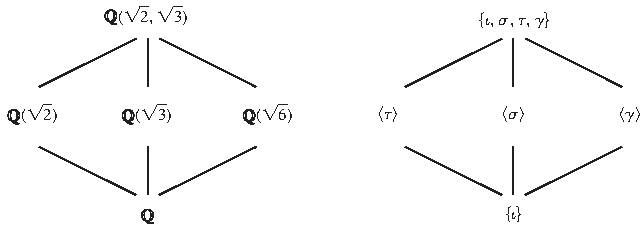
\includegraphics[width=0.882\linewidth,height=.8\textheight,keepaspectratio]{assets/p360_05.pdf}\end{center}
\begin{center}\small\textbf{43.8 Figure}\end{center}
\end{BookFloat}

The fact that the subfield diagram and the subgroup diagram correspond by associating a subfield of \BookInline{K} with a subgroup of \BookInline{G} is no accident. In fact, this is the heart of Galois theory. Before we can give precise statements of the Galois theorems, we need a few definitions and some background lemmas and theorems. It is advisable to have Examples 43.4 and 43.7 well in mind when reading the next few sections.

\BookTextHeading{\textbf{Subfields and Subgroups}  }

\noindent We now investigate the Galois correspondence between subfields and subgroups of the automorphism group of a field. In Example \BookInline{43.7,\allowbreak K} was an extension field of \BookInline{\mathbb{Q}.} In general we will investigate the automorphisms of a field that fix elements of a subfield that is not necessarily the rational numbers.

\BookLabel{43.9 Theorem} Let \BookInline{\sigma } be an automorphism of the field \BookInline{E.} Then the set \BookInline{E_{\sigma }} of all the elements \BookInline{a\in E} that remain fixed by \BookInline{\sigma } forms a subfield of \BookInline{E.}

\BookLabel{\textit{Proof}} Suppose that \BookInline{a,\allowbreak b\in E} remain fixed by \BookInline{\sigma,\allowbreak } that is\BookInline{,\allowbreak \sigma (a)= a} and \BookInline{\sigma (b)= b.} Since \BookInline{\sigma } is a field automorphism, we have

\begin{center}\begin{adjustbox}{max width=\linewidth}\BookInline{\displaystyle \begin{aligned}\sigma (a\pm b)&= \sigma (a)\pm \sigma (b)= a\pm b,\allowbreak  \\ \sigma (ab)&= \sigma (a)\sigma (b)= ab,\allowbreak  \\ \sigma (a/b)&= \sigma (a)/\sigma (b)= a/b\;\text{if}\;b\neq  0,\allowbreak  \\ \sigma (0)&= 0,\allowbreak \;\text{and}\; \\ \sigma (1)&= 1.\end{aligned}}\end{adjustbox}\end{center}

\noindent Thus \BookInline{a\pm b,\allowbreak ab,\allowbreak 0,\allowbreak 1\in E_{\sigma }} and if \BookInline{b\neq 0,\allowbreak a/b\in E_{\sigma },\allowbreak } which imply that \BookInline{E_{\sigma }} is a subfield of\BookInline{E.} \BookEnd{\blacklozenge}

\BookLabel{43.10 Corollary} Let \BookInline{\{\sigma _{i}\mid i\in I\}} be a collection of automorphisms of a field \BookInline{E.} Then the set \BookInline{E_{\{\sigma _{i}\}}}, of all \BookInline{a\in E} that remain fixed by every \BookInline{\sigma _{i},\allowbreak } for \BookInline{i\in I,\allowbreak } is a subfield of \BookInline{E.}

\BookLabel{\textit{Proof}} The set \BookInline{E_{\{\sigma _{i}\}}= \cap _{i\in I}E_{\{\sigma _{i}\}}} is an intersection of subfields of \BookInline{E,\allowbreak } so by Exercise 51 in Section \BookInline{22,\allowbreak E_{\{\sigma _{i}\}}} is a subfield of \BookInline{E.}\BookEnd{\blacklozenge}

We will continue to use the notation \BookInline{E_{\sigma }} to denote the subfield of \BookInline{E} that remains fixed by the automorphism \BookInline{\sigma } and \BookInline{E_{\{\sigma _{i}\}}} to denote the subfield of \BookInline{E} that remains fixed by \BookInline{\sigma _{i}} for every \BookInline{i\in I.}

\BookLabel{43.11 Example} Continuing Example \BookInline{43.7,\allowbreak \mathbb{Q}(\sqrt{2},\allowbreak \sqrt{3})_{\langle \sigma \rangle }= \mathbb{Q}(\sqrt{3})} and \BookInline{\mathbb{Q}(\sqrt{2},\allowbreak \sqrt{3})_{\langle \gamma \rangle }= \mathbb{Q}(\sqrt{6}).} \BookEnd{\blacktriangle}

In the above discussion we started with a set of automorphisms of a field \BookInline{K} and saw that the elements fixed by the automorphisms form a subfield of \BookInline{K.} This provides a way 
% Source PDF page 361; original printed page 344
\BookSource{361}{344}
to assign subfields of \BookInline{K} to subgroups of the group of automorphisms. We now turn our attention to subfields \BookInline{F\leq K} and ask if there is a subgroup of the automorphism group of \BookInline{K} that has exactly the set \BookInline{F} as a fixed set.

\end{BookBody}

\BookNarrativetrue

\begin{BookBody}

\BookLabel{43.12 Definition} Let \BookInline{F\leq K} be a field extension. The set \BookInline{G(K/F)} is the set of all automorphisms of the field \BookInline{K} that fix every element of the field \BookInline{F.}\BookEnd{\blacksquare}

\BookLabel{43.13 Example} We see from Examples 43.4 and 43.7 that

\begin{center}\begin{adjustbox}{max width=\linewidth}\BookInline{\displaystyle \begin{aligned}G(\mathbb{Q}(\sqrt{2},\allowbreak \sqrt{3})/\mathbb{Q}) &= \{\iota,\allowbreak \sigma,\allowbreak \tau,\allowbreak \gamma\} \\G(\mathbb{Q}(\sqrt{2},\allowbreak \sqrt{3})/\mathbb{Q}(\sqrt{3})) &= \{\iota,\allowbreak \sigma\} = \langle \sigma\rangle \\G(\mathbb{Q}(\sqrt{2},\allowbreak \sqrt{3})/\mathbb{Q}(\sqrt{2})) &= \{\iota,\allowbreak \tau\} = \langle \tau\rangle \\G(\mathbb{Q}(\sqrt{2},\allowbreak \sqrt{3})/\mathbb{Q}(\sqrt{6})) &= \{\iota,\allowbreak \gamma\} = \langle \gamma\rangle \\G(\mathbb{Q}(\sqrt{2},\allowbreak \sqrt{3})/\mathbb{Q}(\sqrt{2},\allowbreak \sqrt{3})) &= \{\iota\}.\end{aligned}}\end{adjustbox}\end{center} \BookEnd{\blacktriangle}

If \BookInline{K} is an extension field of \BookInline{F} and \BookInline{F\leq E\leq K,\allowbreak } then we will refer to \BookInline{E} as an\textbf{ in}\textbf{termediate field} of the extension. In Examples 43.11 and 43.13, we saw that for every intermediate field \BookInline{E} of the extension \BookInline{\mathbb{Q}\leq \mathbb{Q}(\sqrt{2},\allowbreak \sqrt{3}),\allowbreak } there was a subgroup \BookInline{H} of the automorphism group of \BookInline{\mathbb{Q}(\sqrt{2},\allowbreak \sqrt{3})} that fixes every element of \BookInline{E} and furthermore, \BookInline{\mathbb{Q}(\sqrt{2},\allowbreak \sqrt{3})_{H}= E.} This one-to-one correspondence between subgroups of the automorphism group and intermediate fields is the essence of Galois theory. There are field extensions where the correspondence fails, as shown by the next example. In order to have this one-to-one correspondence, a few technical conditions on the field extension need to be satisfied.

\BookLabel{43.14 Example} Let \BookInline{K = \mathbb{Q}(\sqrt[3]{2}) = \{ a + b\sqrt[3]{2} + c\sqrt[3]{4} | a,\allowbreak b \in \mathbb{Q} \}}. Then \BookInline{G(K/\mathbb{Q})} consists of all automorphisms of \BookInline{K} that fix all the rational numbers. In \BookInline{\mathbb { Q } ( { \sqrt [ 3 ] { 2 } } )} there is only one zero of the polynomial \BookInline{x^{3}- 2} since the other two zeros, \BookInline{\sqrt[3]{2}(-1\pm\sqrt{3}i)/2,\allowbreak } are complex numbers and \BookInline{\mathbb { Q } ( { \sqrt [ 3 ] { 2 } } )} is a subfield of the real numbers. For any automorphism \BookInline{\sigma \in G(K/\mathbb{Q}),\allowbreak }

\begin{center}\begin{adjustbox}{max width=\linewidth}\BookInline{\displaystyle \begin{aligned}0 &= \sigma(0) = \sigma(\sqrt[3]{2}^3 - 2) \\&= (\sigma(\sqrt[3]{2}))^3 - 2.\end{aligned}}\end{adjustbox}\end{center}

Thus \BookInline{\sigma ( { \sqrt { 2 } } )} is a zero of \BookInline{x^{3}- 2,\allowbreak } which implies that \BookInline{\sigma ( { \sqrt [ 3 ] { 2 } } ) = { \sqrt [ 3 ] { 2 } }.} Therefore any field automorphism of \BookInline{K} fixes all elements of \BookInline{\mathbb{Q}} and \BookInline{\sqrt { 2 }} which implies that the only automorphism of \BookInline{K} is the identity automorphism \BookInline{\iota.} Thus \BookInline{G(K/\mathbb{Q})= \{\iota \}} and \BookInline{K_{G(K/\mathbb{Q})}= K_{\{\iota \}}= K.} In this case, there is no subgroup \BookInline{H\leq G(K/\mathbb{Q})} with \BookInline{K_{H}= \mathbb{Q}.}\BookEnd{\blacktriangle}

In the next two sections, we will investigate conditions on field extensions \BookInline{F\leq K} where there is a one-to-one correspondence between the intermediate fields and the subgroups of G\BookInline{(K/F).}

\BookLabel{43.15 Theorem} Let \BookInline{E} be a field and let \BookInline{F} be a subfield of \BookInline{E.} Then the set \BookInline{G(E/F)} of all automorphisms that fix all the elements of \BookInline{F} is a subgroup of the automorphism group of \BookInline{E.} Furthermore\BookInline{,\allowbreak F} is a subfield of \BookInline{E_{G(E/F)}.}

\BookLabel{\textit{Proof}} For \BookInline{\sigma,\allowbreak \tau \in G(E/F)} and \BookInline{a\in F,\allowbreak }

\begin{center}\begin{adjustbox}{max width=\linewidth}\BookInline{\displaystyle (\sigma \tau )(a)= \sigma (\tau (a))= \sigma (a)= a,\allowbreak }\end{adjustbox}\end{center}

\noindent so \BookInline{\sigma \tau \in G(E/F).} Furthermore\BookInline{,\allowbreak G(E/F)} contains the identity map and \BookInline{\sigma ^{- 1}(a)= a.} Thus \BookInline{G(E/F)} is a subgroup of the automorphisms of \BookInline{E.}

Finally, since every automorphism in \BookInline{G(E/F)} fixes all the elements of \BookInline{F,\allowbreak F} is a subset and, therefore, a subfield of \BookInline{E_{G(E/F)}.}\BookEnd{\blacklozenge}

\end{BookBody}

% Source PDF page 362; original printed page 345
\BookSource{362}{345}
\BookNarrativetrue

\begin{BookBody}

Since \BookInline{G(E/F)} is a subgroup of the automorphisms of \BookInline{E,\allowbreak } we naturally call \BookInline{G(E/F)} the\textbf{ group of automorphisms of} \BookInline{E} \textbf{that fix} \BookInline{F.} More briefly, we say that \BookInline{G(E/F)} is the \textbf{group of} \BookInline{E} \textbf{over} \BookInline{F.}

Beware! The symbol “/” in \BookInline{G(E/F)} does not refer to a fraction or a quotient space. The symbol “/” is used since we read \BookInline{G(E/F)} as the group of \BookInline{E} \textit{over} \BookInline{F} and in the subfield diagram\BookInline{,\allowbreak E} is written above \BookInline{F.}

Since \BookInline{G(E/F)} is a subgroup of the automorphisms of \BookInline{E,\allowbreak } we naturally call \BookInline{G(E/F)} the\textbf{ group of automorphisms of} \BookInline{E} \textbf{that fix} \BookInline{F.} More briefly, we say that \BookInline{G(E/F)} is the \textbf{group of} \BookInline{E} \textbf{over} \BookInline{F.}

Beware! The symbol “/” in \BookInline{G(E/F)} does not refer to a fraction or a quotient space. The symbol “/” is used since we read \BookInline{G(E/F)} as the group of \BookInline{E} \textit{over} \BookInline{F} and in the subfield diagram\BookInline{,\allowbreak E} is written above \BookInline{F.}

\BookTextHeading{\textbf{Conjugation Isomorphisms}  }

In our ongoing example of \BookInline{K= \mathbb{Q}(\sqrt{2},\allowbreak \sqrt{3}),\allowbreak } we noticed that for any automorphism \BookInline{\sigma } of \BookInline{K,\allowbreak \sigma (\sqrt{2})= \pm \sqrt{2}} since the image of a zero of \BookInline{x^{2}- 2} must also be a zero of \BookInline{x^{2}- 2.} This observation can be used for any polynomial and it is the basis for the Conjugation Theorem.

\BookLabel{43.16 Definition} Let \BookInline{E} be an algebraic extension of the field \BookInline{F.} Two elements \BookInline{\alpha } and \BookInline{\beta } in \BookInline{E} are \textbf{conjugates over} \BookInline{F,\allowbreak } if both have the same minimal polynomial over \BookInline{F.} That is, irr\BookInline{(\alpha,\allowbreak F)= } irr\BookInline{(\beta,\allowbreak F).}\BookEnd{\blacksquare}

\BookLabel{43.17 Example} The definition of conjugates over \BookInline{F} is consistent with our familiar use of the term complex conjugates in the setting of complex numbers. For \BookInline{a,\allowbreak b\in \mathbb{R},\allowbreak } the numbers \BookInline{a+ } \textit{bi} and \BookInline{a- } \textit{bi} are complex conjugates. Both are zeros of the polynomial \BookInline{f(x)= x^{2}- 2}\textit{ax} \BookInline{+ } \BookInline{a^{2}+ b^{2}} and, as long as \BookInline{b\neq 0,\allowbreak f(x)} is irreducible over \BookInline{\mathbb{R}.} Thus for \BookInline{b\neq 0,\allowbreak a+ } \textit{bi} and \BookInline{a- } \textit{bi} have the same minimal polynomial and they are conjugates over \BookInline{\mathbb{R}} in the sense of Definition \BookInline{43.16.}\BookEnd{\blacktriangle}

\BookLabel{43.18 Theorem} \textbf{(The Conjugation Isomorphism)} Let \BookInline{F} be a field\BookInline{,\allowbreak K} an extension field of \BookInline{F,\allowbreak } and \BookInline{\alpha,\allowbreak \beta \in K} algebraic over \BookInline{F} with deg\BookInline{(\alpha,\allowbreak F)= n.} The map \BookInline{\psi _{\alpha,\allowbreak \beta }:F(\alpha )\to F(\beta )} defined by

\begin{center}\begin{adjustbox}{max width=\linewidth}\BookInline{\displaystyle \psi _{\alpha ,\allowbreak \beta }(c_{0}+ c_{1}\alpha + c_{2}\alpha ^{2}+ \cdots + c_{n- 1}\alpha ^{n- 1})= c_{0}+ c_{1}\beta + c_{2}\beta ^{2}+ \cdots + c_{n- 1}\beta ^{n- 1},\allowbreak }\end{adjustbox}\end{center}

\noindent for \BookInline{c_{i}\in F,\allowbreak } is an isomorphism of \BookInline{F(\alpha )} onto \BookInline{F(\beta )} if and only if \BookInline{\alpha } and \BookInline{\beta } are conjugate over \BookInline{F.}

\BookLabel{\textit{Proof}} We first assume that \BookInline{\psi _{\alpha,\allowbreak \beta }} is an isomorphism. Since deg\BookInline{(\alpha,\allowbreak F)= n,\allowbreak } irr\BookInline{(\alpha,\allowbreak F)= x^{n}+ g(x),\allowbreak } for some polynomial \BookInline{g(x)\in F[x],\allowbreak } where the degree of \BookInline{g(x)} is less than \BookInline{n.} Therefore

\begin{center}\begin{adjustbox}{max width=\linewidth}\BookInline{\displaystyle \alpha ^{n}= - g(\alpha ).}\end{adjustbox}\end{center}

\noindent Since \BookInline{\psi _{\alpha,\allowbreak \beta }} is an isomorphism,

\begin{center}\begin{adjustbox}{max width=\linewidth}\BookInline{\displaystyle \psi _{\alpha ,\allowbreak \beta }(\alpha ^{n})= (\psi _{\alpha ,\allowbreak \beta }(\alpha ))^{n}= \beta ^{n}.}\end{adjustbox}\end{center}

\noindent On the other hand,

\begin{center}\begin{adjustbox}{max width=\linewidth}\BookInline{\displaystyle \psi _{\alpha ,\allowbreak \beta }(g(\alpha ))= g(\beta ).}\end{adjustbox}\end{center}

\noindent Thus

\begin{center}\begin{adjustbox}{max width=\linewidth}\BookInline{\displaystyle \beta ^{n}= \psi _{\alpha ,\allowbreak \beta }(\alpha ^{n})= \psi _{\alpha ,\allowbreak \beta }(- g(\alpha ))= - g(\beta ).}\end{adjustbox}\end{center}

\noindent So \BookInline{\beta } is a zero of the polynomial \BookInline{x^{n}+ g(x)= } irr\BookInline{(\alpha,\allowbreak F),\allowbreak } which is irreducible over \BookInline{F.} By the definition of the minimal polynomial, irr\BookInline{(\beta,\allowbreak F)= x^{n}+ g(x)= } irr\BookInline{(\alpha,\allowbreak F).}

\end{BookBody}

% Source PDF page 363; original printed page 346
\BookSource{363}{346}
\BookNarrativetrue

\begin{BookBody}

We next assume that \BookInline{\alpha } and \BookInline{\beta } are conjugates over \BookInline{F} with minimal polynomial \BookInline{p(x)= } irr\BookInline{(\alpha,\allowbreak F)= } irr\BookInline{(\beta,\allowbreak F).} By Corollary 39.14, the ideal \BookInline{\langle p(x)\rangle \subseteq F[x]} is the kernel of the evaluation homomorphism \BookInline{\phi _{\alpha }:F[x]\to F(\alpha ),\allowbreak } which is onto. By the Fundamental Homomorphism Theorem 30.17, there is an isomorphism \BookInline{\psi _{\alpha }:F[x]/\langle p(x)\rangle \to F(\alpha )} with \BookInline{\psi _{\alpha }(a+ \langle p(x)\rangle )= a} for all \BookInline{a\in F} and \BookInline{\psi _{\alpha }(x+ \langle p(x)\rangle )= \alpha.} Similarly, there is an isomorphism \BookInline{\psi _{\beta }:F[x]/\langle p(x)\rangle \to F(\beta )} with \BookInline{\psi _{\beta }(a+ \langle p(x)\rangle )= a} for all \BookInline{a\in F,\allowbreak } and \BookInline{\psi _{\beta }(x+ } \BookInline{\langle p(x)\rangle )= \beta.} Since \BookInline{\psi _{\alpha }} and \BookInline{\psi _{\beta }} are both isomorphisms\BookInline{,\allowbreak \psi _{\alpha }^{- 1}:F(\alpha )\to F[x]/\langle p(x)\rangle } is an isomorphism and \BookInline{\psi _{\alpha,\allowbreak \beta }= \psi _{\beta }\circ \psi _{\alpha }^{- 1}:F(\alpha )\to F(\beta )} is also an isomorphism. We have

\begin{center}\begin{adjustbox}{max width=\linewidth}\BookInline{\displaystyle \begin{aligned}\psi _{\alpha ,\allowbreak \beta }(\alpha )&= \psi _{\beta }(\psi _{\alpha }^{- 1}(\alpha ) \\ &= \psi _{\beta }(x+ \langle p(x)\rangle ) \\ &= \beta .\end{aligned}}\end{adjustbox}\end{center}

We also note that for \BookInline{c\in F,\allowbreak \psi _{\alpha,\allowbreak \beta }(c)= c.} Let \BookInline{c_{0},\allowbreak c_{1},\allowbreak...,\allowbreak c_{n- 1}\in F} since \BookInline{\psi _{\alpha,\allowbreak \beta }} is an isomorphism,

\begin{center}\begin{adjustbox}{max width=\linewidth}\BookInline{\displaystyle \begin{aligned}&\psi _{\alpha ,\allowbreak \beta }(c_{0}+ c_{1}\alpha + ...+ c_{n- 1}\alpha ^{n- 1}) \\ &= \psi _{\alpha ,\allowbreak \beta }(c_{0})+ \psi _{\alpha ,\allowbreak \beta }(c_{1})\psi _{\alpha ,\allowbreak \beta }(\alpha )+ \cdots + \psi _{\alpha ,\allowbreak \beta }(c_{n- 1})\psi _{\alpha ,\allowbreak \beta }(\alpha ^{n- 1}) \\ &= c_{0}+ c_{1}\psi _{\alpha ,\allowbreak \beta }(\alpha )+ \cdots + c_{n- 1}\psi _{\alpha ,\allowbreak \beta }(\alpha )^{n- 1} \\ &= c_{0}+ c_{1}\beta + \cdots + c_{n- 1}\beta ^{n- 1}.\end{aligned}}\end{adjustbox}\end{center} \BookEnd{\blacklozenge}

\BookLabel{43.19 Corollary} Let \BookInline{K} be a field extension of \BookInline{F} with \BookInline{\alpha \in K} algebraic over \BookInline{F.} Suppose that \BookInline{\psi } is an isomorphism of \BookInline{F(\alpha )} onto a subfield of \BookInline{K,\allowbreak } with the property that every element of \BookInline{F} is fixed by \BookInline{\psi.} Then \BookInline{\psi } maps \BookInline{\alpha } to a conjugate over \BookInline{F} of \BookInline{\alpha.} Conversely, if \BookInline{\beta \in K} is conjugate over \BookInline{F} with \BookInline{\alpha,\allowbreak } then there is a unique isomorphism \BookInline{\psi _{\alpha,\allowbreak \beta }} mapping \BookInline{F(\alpha )} onto a subfield of \BookInline{K} with the properties that each \BookInline{a\in F} is fixed by \BookInline{\sigma } and \BookInline{\sigma (\alpha )= \beta.}

\BookLabel{\textit{Proof}} Let \BookInline{\psi } be an isomorphism from \BookInline{F(\alpha )} onto a subfield of \BookInline{K} with the property that every element of \BookInline{F} is fixed by \BookInline{\psi.} Let irr\BookInline{(\alpha,\allowbreak F)= a_{0}+ a_{1}x+ \cdots + a_{n- 1}x^{n- 1}.} Then

\begin{center}\begin{adjustbox}{max width=\linewidth}\BookInline{\displaystyle a_{0}+ a_{1}\alpha + ...a_{n- 1}\alpha ^{n- 1}= 0}\end{adjustbox}\end{center}

\noindent and

\begin{center}\begin{adjustbox}{max width=\linewidth}\BookInline{\displaystyle 0= \psi (a_{0}+ a_{1}\alpha + \cdots + a_{n- 1}\alpha ^{n- 1})= a_{0}+ a_{1}\psi (\alpha )+ \cdots + a_{n- 1}\psi (\alpha )^{n- 1}.}\end{adjustbox}\end{center}

\noindent Thus \BookInline{\beta = \psi (\alpha )} has minimal polynomial \BookInline{a_{0}+ a_{1}x+ \cdots + a_{n- 1}x^{n- 1}} over \BookInline{F,\allowbreak } which says that \BookInline{\alpha } and \BookInline{\beta } are conjugates over \BookInline{F.}

Now we let \BookInline{\beta \in K} be a conjugate of \BookInline{\alpha } over \BookInline{F.} Theorem 43.18 provides an isomorphism \BookInline{\psi _{\alpha,\allowbreak \beta }:F(\alpha )\to F(\beta )} with the desired properties. Uniqueness follows since any isomorphism from \BookInline{F(\alpha )} to any field is completely determined by its values on elements of \BookInline{F} and its value on \BookInline{\alpha.}\BookEnd{\blacklozenge}

Theorem 43.9 and Corollary 43.19 formalize ideas used in Examples 43.7 and 43.14. Any automorphism \BookInline{\sigma } of \BookInline{\widehat{\mathbb{Q}}(\sqrt{2},\allowbreak \sqrt{3})} when restricted to the subfield \BookInline{\mathbb{Q}(\sqrt{2})} is an isomorphism onto a subfield of \BookInline{\mathbb{Q}(\sqrt{2},\allowbreak \sqrt{3})}. Corollary 43.19 states that the automorphism maps \BookInline{{ \sqrt { 2 } } \; \mathrm { t o } \pm { \sqrt { 2 } }} Similarly \BookInline{\sqrt{3}} maps to \BookInline{\pm \sqrt{3},\allowbreak } making a total of at most four automorphisms of \BookInline{\mathbb{Q}(\sqrt{2},\allowbreak \sqrt{3}).}

Looking back at Example 43.14, any automorphism of \BookInline{\mathbb { Q } ( { \sqrt [ 3 ] { 2 } } )} maps \BookInline{\sqrt { 2 }} to a conjugate over \BookInline{\mathbb{Q}} and fixes elements of \BookInline{\mathbb{Q}.} But \BookInline{\sqrt { 2 }} has no conjugates in \BookInline{\mathbb { Q } ( { \sqrt [ 3 ] { 2 } } )} other than itself, so the only automorphism of \BookInline{\mathbb { Q } ( { \sqrt [ 3 ] { 2 } } )} is the identity map. Corollary 43.19 is essential for the rest of our study of Galois theory.

We now give a familiar corollary of Theorem 43.18 concerning complex number zeros of polynomials with real coefficients. Corollary 43.20 states that complex zeros of polynomials with real coefficients occur in conjugate pairs.

\end{BookBody}

% Source PDF page 364; original printed page 347
\BookSource{364}{347}
\BookNarrativetrue

\begin{BookBody}

\BookLabel{43.20 Corollary} Let \BookInline{f(x)\in \mathbb{R}[x].} If \BookInline{a,\allowbreak b\in \mathbb{R}} and \BookInline{f(a+ } \textit{bi}\BookInline{)\; = 0,\allowbreak } then \BookInline{f(a- } \textit{bi}\BookInline{)\; = 0.}

\BookLabel{\textit{Proof}} As a field \BookInline{\mathbb{C}= \mathbb{R}(i).} Both \BookInline{i} and \BookInline{- i} have minimal polynomial \BookInline{x^{2}+ 1} over \BookInline{\mathbb{R},\allowbreak } so they are conjugate over \BookInline{R.} Theorem 43.18 assures us that there is an automorphism \BookInline{\psi _{i,\allowbreak - i}:} \BookInline{\mathbb{R}(i)= \mathbb{C}\to \mathbb{C}} given by \BookInline{\psi _{i,\allowbreak - i}(a+ ib)= a- } \textit{bi}. Let

\begin{center}\begin{adjustbox}{max width=\linewidth}\BookInline{\displaystyle f(x)= a_{0}+ a_{1}x+ a_{2}x^{2}+ \cdots + a_{n}x^{n}}\end{adjustbox}\end{center}

\noindent and assume that \BookInline{a+ } \textit{bi} is a zero of \BookInline{f(x).} Then

\begin{center}\begin{adjustbox}{max width=\linewidth}\BookInline{\displaystyle 0= f(a+ bi)= a_{0}+ a_{1}(a+ bi)+ a_{2}(a+ bi)^{2}+ \cdots + a_{n}(a+ bi)^{n},\allowbreak }\end{adjustbox}\end{center}

\noindent so

\begin{center}\begin{adjustbox}{max width=\linewidth}\BookInline{\displaystyle 0= \psi _{i,\allowbreak - i}(f(a+ bi))= a_{0}+ a_{1}(a- bi)+ a_{2}(a- bi)^{2}+ \cdots + a_{n}(a- bi)^{n}= f(a- bi).}\end{adjustbox}\end{center}

\noindent Thus \BookInline{f(a- } \textit{bi}\BookInline{)\; = 0.} \BookEnd{\blacklozenge}

In order to pursue the Galois connection between subgroups of \BookInline{G(K/F)} and intermediate fields \BookInline{F\leq E\leq K,\allowbreak } we need a technical condition to be sure that \BookInline{K} has enough conjugate elements so Theorem 43.18 and its Corollary 43.19 can be evoked as often as needed. When the technical condition on \BookInline{E} is satisfied, then \BookInline{E} is called a\textbf{ splitting field}. We investigate splitting fields in Section 44.

There is one other technical condition that we will need in order to establish the Galois correspondence. That condition says that for each \BookInline{\alpha \in K,\allowbreak } irr\BookInline{(\alpha,\allowbreak F)} has deg\BookInline{(\alpha,\allowbreak F)} distinct zeros in the algebraic closure of \BookInline{K.} If the field extension \BookInline{E} over \BookInline{F} satisfies this condition, then the extension is said to be\textbf{ separable}. As we will see, essentially all of our applications and examples, as well as most field extensions with which we are familiar, are separable. But we are getting ahead of ourselves, as properties of separable extensions are the focus of Section 45.

\end{BookBody}

\BookNarrativefalse

\begin{BookBody}

\BookExerciseTitle{43}

\BookTextHeading{\textbf{Computations}}

\noindent In Exercises 1 through 8, find all conjugates in \BookInline{\mathbb{C}} of the given number over the given field.

\BookExercise{1.}{\BookInline{\sqrt{2}} over \BookInline{\mathbb{Q}}}

\BookExercise{2.}{\BookInline{\sqrt{2}} over \BookInline{\mathbb{R}}}

\BookExercise{3.}{\BookInline{3+ \sqrt{2}} over \BookInline{\mathbb{Q}}}

\BookExercise{4.}{\BookInline{\sqrt{2}- \sqrt{3}} over \BookInline{\mathbb{Q}}}

\BookExercise{5.}{\BookInline{\sqrt{2}+ i} over \BookInline{\mathbb{Q}}}

\BookExercise{6.}{\BookInline{\sqrt{2}+ i} over \BookInline{\mathbb{R}}}

\BookExercise{7.}{\BookInline{\sqrt{1}+ \sqrt{2}} over \BookInline{\mathbb{Q}}}

\BookExercise{8.}{\BookInline{\sqrt{1}+ \sqrt{2}} over \BookInline{\mathbb{Q}(\sqrt{2})}}

In Exercises 9 through 15, we consider the field \BookInline{E= \mathbb{Q}(\sqrt{2},\allowbreak \sqrt{3},\allowbreak \sqrt{5}).} It can be shown that \BookInline{[E:\mathbb{Q}]= 8.} In the notation of Theorem 43.18, we have the following conjugation isomorphisms (which are here automorphisms of \BookInline{E):}

\begin{center}\begin{adjustbox}{max width=\linewidth}\BookInline{\displaystyle \psi _ { \sqrt { 2 } ,\allowbreak  - \sqrt { 2 } } : ( \mathbb { Q } ( \sqrt { 3 } ,\allowbreak  \sqrt { 5 } ) ) ( \sqrt { 2 } ) \to ( \mathbb { Q } ( \sqrt { 3 } ,\allowbreak  \sqrt { 5 } ) ) ( - \sqrt { 2 } ) ,\allowbreak }\end{adjustbox}\end{center}

\begin{center}\begin{adjustbox}{max width=\linewidth}\BookInline{\displaystyle \psi _ { \sqrt { 3 } ,\allowbreak  - \sqrt { 3 } } : ( \mathbb { Q } ( \sqrt { 2 } ,\allowbreak  \sqrt { 5 } ) ) ( \sqrt { 3 } ) \to ( \mathbb { Q } ( \sqrt { 2 } ,\allowbreak  \sqrt { 5 } ) ) ( - \sqrt { 3 } ) ,\allowbreak }\end{adjustbox}\end{center}

\begin{center}\begin{adjustbox}{max width=\linewidth}\BookInline{\displaystyle \psi _ { \sqrt { 5 } ,\allowbreak  - \sqrt { 5 } } : ( \mathbb { Q } ( \sqrt { 2 } ,\allowbreak  \sqrt { 3 } ) ) ( \sqrt { 5 } ) \to ( \mathbb { Q } ( \sqrt { 2 } ,\allowbreak  \sqrt { 3 } ) ) ( - \sqrt { 5 } ) .}\end{adjustbox}\end{center}

\noindent For shorter notation, let \BookInline{\tau _ { 2 } = \psi _ { \sqrt { 2 },\allowbreak - \sqrt { 2 } },\allowbreak \tau _ { 3 } = \psi _ { \sqrt { 3 },\allowbreak - \sqrt { 3 } },\allowbreak } and \BookInline{\tau _ { 5 } = \psi _ { \sqrt { 5 },\allowbreak - \sqrt { 5 } }} Compute the indicated element of \BookInline{E.}

\BookExercise{9.}{\BookInline{\tau _{2}(\sqrt{3})}}

\BookExercise{10.}{\BookInline{\tau _ { 2 } ( { \sqrt { 2 } } + { \sqrt { 5 } } )}}

\BookInline{\left( \tau _ { 5 } \tau _ { 3 } \right) \left( \frac { \sqrt { 2 } - 3 \sqrt { 5 } } { 2 \sqrt { 3 } - \sqrt { 2 } } \right)}

\BookExercise{11.}{\BookInline{(\tau _{3}\tau _{2})(\sqrt{2}+ 3\sqrt{5})}}

\BookExercise{12.}{\BookInline{\left( \tau _ { 5 } \tau _ { 3 } \right) \left( \frac { \sqrt { 2 } - 3 \sqrt { 5 } } { 2 \sqrt { 3 } - \sqrt { 2 } } \right)}}

\BookExercise{13.}{\BookInline{(\tau _{5}^{2}\tau _{3}\tau _{2})(\sqrt{2}+ \sqrt{45})}}

\BookExercise{14.}{\BookInline{\tau _{3}[\tau _{5}(\sqrt{2}- \sqrt{3}+ (\tau _{2}\tau _{5})(\sqrt{30}))]}}

\end{BookBody}

% Source PDF page 365; original printed page 348
\BookSource{365}{348}
\BookNarrativefalse

\begin{BookBody}

\BookExercise{15.}{\BookInline{\tau _{3}\tau _{5}\tau _{3}^{- 1}(\sqrt{3}- \sqrt{5})}}

\noindent In Exercises 16 through 21, refer to the directions for Exercises 9 through 15 and find the fixed field of the automorphism or set of automorphisms of \BookInline{E.}

\BookExercise{16.}{\BookInline{\tau _{3}}}

\BookExercise{17.}{2 \BookInline{\tau } 3}

\BookExercise{18.}{\BookInline{\{\tau _{2},\allowbreak \tau _{3}\}}}

\BookExercise{19.}{\BookInline{\tau _{5}\tau _{2}}}

\BookExercise{20.}{\BookInline{\tau _{5}\tau _{3}\tau _{2}}}

\BookExercise{21.}{\BookInline{\{\tau _{2},\allowbreak \tau _{3},\allowbreak \tau _{5}\}}}

\BookExercise{22.}{Refer to the directions for Exercises 9 through 15 for this exercise.}

\BookExercise{a.}{Show that each of the automorphisms \BookInline{\tau _{2},\allowbreak \tau _{3},\allowbreak } and \BookInline{\tau _{5}} is of order 2 in \BookInline{G(E/\mathbb{Q}).(}Remember what is meant by the\textit{ order} of an element of a group.)}

\BookExercise{b.}{Find the subgroup \BookInline{H} of \BookInline{G(E/\mathbb{Q})} generated by the elements \BookInline{\tau _{2},\allowbreak \tau _{3},\allowbreak } and \BookInline{\tau _{5},\allowbreak } and give the group table. [\textit{Hint:} There are eight elements.]}

\BookExercise{c.}{Just as was done in Example 43.4, argue that the group \BookInline{H} of part (b) is the full group \BookInline{G(E/\mathbb{Q}).}}

\BookTextHeading{\textbf{Concepts}}

\noindent In Exercises 23 and 24, correct the definition of the italicized term without reference to the text, if correction is needed, so that it is in a form acceptable for publication.

\BookExercise{23.}{Two elements\BookInline{,\allowbreak \alpha } and \BookInline{\beta,\allowbreak } of an algebraic extension \BookInline{E} of a field \BookInline{F} are\textit{ conjugate over} \BookInline{F} if and only if they are both zeros of the same polynomial \BookInline{f(x)} in \BookInline{F[x].}}

\BookExercise{24.}{Two elements\BookInline{,\allowbreak \alpha } and \BookInline{\beta,\allowbreak } of an algebraic extension \BookInline{E} of a field \BookInline{F} are\textit{ conjugate over} \BookInline{F} if and only if the evaluation homomorphisms \BookInline{\phi _{\alpha }:F[x]\to E} and \BookInline{\phi _{\beta }:F[x]\to E} have the same kernel.}

\BookExercise{25.}{The fields \BookInline{\mathbb{Q}(\sqrt{2})} and \BookInline{\mathbb{Q}(3+ \sqrt{2})} are the same, of course. Let \BookInline{\alpha = 3+ \sqrt{2}.}}

\BookExercise{a.}{Find a conjugate \BookInline{\beta \neq \alpha } of \BookInline{\alpha } over \BookInline{\mathbb{Q}.}}

\textbf{b.} Referring to part (a), compare the conjugation automorphism \BookInline{\psi _ { \sqrt { 2 },\allowbreak - \sqrt { 2 } }} of \BookInline{\mathbb{Q}(\sqrt{2})} with the conjugation automorphism \BookInline{\psi _{\alpha,\allowbreak \beta }.}

\BookExercise{26.}{Determine whether each of the following is true or false.}

\BookExercise{a.}{For all \BookInline{\alpha,\allowbreak \beta \in E,\allowbreak } there is always an automorphism of \BookInline{E} mapping \BookInline{\alpha } onto \BookInline{\beta.}}

\BookExercise{b.}{For \BookInline{\alpha,\allowbreak \beta } algebraic over a field \BookInline{F,\allowbreak } there is always an isomorphism of \BookInline{F(\alpha )} onto \BookInline{F(\beta ).}}

\BookExercise{c.}{For \BookInline{\alpha,\allowbreak \beta } algebraic and conjugate over a field \BookInline{F,\allowbreak } there is always an isomorphism of \BookInline{F(\alpha )} onto \BookInline{F(\beta ).}}

\BookExercise{d.}{Every automorphism of every field \BookInline{E} fixes every element of the prime subfield of \BookInline{E.}}

\BookExercise{e.}{Every automorphism of every field \BookInline{E} fixes an infinite number of elements of \BookInline{E.}}

\BookExercise{f.}{Every automorphism of every field \BookInline{E} fixes at least two elements of \BookInline{E.}}

\BookExercise{g.}{Every automorphism of every field \BookInline{E} of characteristic 0 fixes an infinite number of elements of \BookInline{E.}}

\BookExercise{h.}{All automorphisms of a field \BookInline{E} form a group under function composition.}

\BookExercise{i.}{The set of all elements of a field \BookInline{E} fixed by a single automorphism of \BookInline{E} forms a subfield of \BookInline{E.}}

\BookExercise{j.}{For fields \BookInline{F\leq E\leq K,\allowbreak G(K/E)\leq G(K/F).}}

\BookLabel{\textit{Proof}} \textbf{ Synopsis}

\BookExercise{27.}{Give a one-sentence synopsis of the “if” part of Theorem 43.18.}

\BookExercise{28.}{Give a one-sentence synopsis of the “only if” part of Theorem 43.18.}

\BookTextHeading{\textbf{Theory}}

\BookExercise{29.}{Prove Theorem 43.2.}

\BookExercise{30.}{Show that the only subfields of \BookInline{\mathbb{Q}(\sqrt{2},\allowbreak \sqrt{3})} are \BookInline{\mathbb{Q},\allowbreak \mathbb{Q}(\sqrt{2}),\allowbreak \mathbb{Q}(\sqrt{3}),\allowbreak \mathbb{Q}(\sqrt{6}),\allowbreak } and \BookInline{\mathbb { Q } ( { \sqrt { 2 } },\allowbreak { \sqrt { 3 } } )}. [Hint: Show that a subfield of \BookInline{\mathbb{Q}(\sqrt{2},\allowbreak \sqrt{3})} that is a degree 2 extension of \BookInline{\mathbb{Q}} must be of the form \BookInline{\mathbb{Q}(\sqrt{s})} for some rational number \BookInline{s.]}}

\BookExercise{31.}{Let \BookInline{\alpha } be algebraic of degree \BookInline{n} over \BookInline{F.} Show that there are at most \BookInline{n} different isomorphisms of \BookInline{F(\alpha )} onto a subfield of \BookInline{\overline{F}} and leaving \BookInline{F} fixed.}

\BookExercise{32.}{Let \BookInline{F(\alpha _{1},\allowbreak \cdots,\allowbreak \alpha _{n})} be an extension field of \BookInline{F.} Show that any automorphism \BookInline{\sigma } of \BookInline{F(\alpha _{1},\allowbreak \cdots,\allowbreak \alpha _{n})} leaving \BookInline{F} fixed is completely determined by the \BookInline{n} values \BookInline{\sigma (\alpha _{i}).}}

\end{BookBody}

% Continuation on source PDF page 366, preceding Section 44
\BookNarrativefalse

\begin{BookBody}

\BookExercise{33.}{Let \BookInline{E} be an algebraic extension of a field \BookInline{F,\allowbreak } and let \BookInline{\sigma } be an automorphism of \BookInline{E} leaving \BookInline{F} fixed. Let \BookInline{\alpha \in E.} Show that \BookInline{\sigma } induces a permutation of the set of all zeros of irr\BookInline{(\alpha,\allowbreak F)} that are in \BookInline{E.}}

\BookExercise{34.}{Let \BookInline{E} be an algebraic extension of a field \BookInline{F.} Let \BookInline{S= \{\sigma _{i}\mid i\in I\}} be a collection of automorphisms of \BookInline{E} such that every \BookInline{\sigma _{i}} leaves each element of \BookInline{F} fixed. Show that if \BookInline{S} generates the subgroup \BookInline{H} of \BookInline{G(E/F),\allowbreak } then \BookInline{E_{S}= E_{H}.}}

\BookExercise{35.}{Let \BookInline{F} be a finite field with characteristic \BookInline{p.} Prove that the map \BookInline{\phi:F\to F} defined by \BookInline{\phi (\alpha )= \alpha ^{p}} is a field automorphism. This automorphism is called the\textbf{ Frobenius automorphism}.}

\BookExercise{36.}{Referring to Exercise 35, let \BookInline{F} be a finite field of characteristic \BookInline{p,\allowbreak } and let \BookInline{\phi } be the Frobenius automorphism on \BookInline{F.} Prove that the fixed field \BookInline{F_{\{\phi \}}} is isomorphic with \BookInline{\mathbb{Z}_{p}.}}

\BookExercise{37.}{Referring to Exercise 35, show that the finite assumption is necessary by finding an example of a field \BookInline{F} with characteristic \BookInline{p,\allowbreak } such that the map \BookInline{\phi:F\to F} given by \BookInline{\phi (\alpha )= \alpha ^{p}} is not an automorphism.}

\BookExercise{38.}{We saw in Corollary 28.18 that the cyclotomic polynomial}

\begin{center}\begin{adjustbox}{max width=\linewidth}\BookInline{\displaystyle \Phi _ { p } ( x ) = { \frac { x ^ { p - 1 } } { x - 1 } } = x ^ { p - 1 } + x ^ { p - 2 } + \cdots + x + 1}\end{adjustbox}\end{center}

\noindent is irreducible over \BookInline{\mathbb{Q}} for every prime \BookInline{p.} Let \BookInline{\zeta } be a zero of \BookInline{\Phi _{p}(x),\allowbreak } and consider the field \BookInline{\mathbb{Q}(\zeta ).}

\BookExercise{a.}{Show that \BookInline{\zeta,\allowbreak \zeta ^{2},\allowbreak \cdots,\allowbreak \zeta ^{p- 1}} are distinct zeros of \BookInline{\Phi _{p}(x),\allowbreak } and conclude that they are all the zeros of \BookInline{\Phi _{p}(x).}}

\BookExercise{b.}{Deduce from Corollary 43.19 and part (a) of this exercise that \BookInline{G(\mathbb{Q}(\zeta )/\mathbb{Q})} is abelian of order \BookInline{p- 1.}}

\BookExercise{c.}{Show that the fixed field of \BookInline{G(\mathbb{Q}(\zeta )/\mathbb{Q})} is \BookInline{\mathbb{Q}.[}\textit{Hint:} Show that}

\begin{center}\begin{adjustbox}{max width=\linewidth}\BookInline{\displaystyle \{\zeta ,\allowbreak \zeta ^{2},\allowbreak \cdots ,\allowbreak \zeta ^{p- 1}\}}\end{adjustbox}\end{center}

is a basis for \BookInline{\mathbb{Q}(\zeta )} over \BookInline{\mathbb{Q},\allowbreak } and consider which linear combinations of \BookInline{\zeta,\allowbreak \zeta ^{2},\allowbreak \cdots,\allowbreak \zeta ^{p- 1}} are fixed by all elements of \BookInline{G(\mathbb{Q}(\zeta )/\mathbb{Q}).}

\BookExercise{39.}{Theorem 43.18 described conjugation isomorphisms for the case where \BookInline{\alpha } and \BookInline{\beta } were conjugate algebraic elements over \BookInline{F.} Is there a similar isomorphism of \BookInline{F(\alpha )} with \BookInline{F(\beta )} in the case that \BookInline{\alpha } and \BookInline{\beta } are both transcendental over \BookInline{F}?}

\BookExercise{40.}{Let \BookInline{F} be a field, and let \BookInline{x} be an indeterminate over \BookInline{F.} Determine all automorphisms of \BookInline{F(x)} leaving \BookInline{F} fixed, by describing their values on \BookInline{x.}}

\BookExercise{41.}{Prove the following sequence of theorems.}

\BookExercise{a.}{An automorphism of a field \BookInline{E} carries elements that are squares of elements in \BookInline{E} onto elements that are squares of elements of \BookInline{E.}}

\BookExercise{b.}{An automorphism of the field \BookInline{\mathbb{R}} of real numbers carries positive numbers onto positive numbers.}

\BookExercise{c.}{If \BookInline{\sigma } is an automorphism of \BookInline{\mathbb{R}} and \BookInline{a<b,\allowbreak } where \BookInline{a,\allowbreak b\in \mathbb{R},\allowbreak } then \BookInline{\sigma (a)<\sigma (b).}}

\BookExercise{d.}{The only automorphism of \BookInline{\mathbb{R}} is the identity automorphism.}

\end{BookBody}
\ifdefined\BookMaster\let\BookFinish\relax\else\def\BookFinish{\end{document}}\fi\BookFinish

\clearpage
% !TeX program = xelatex
\ifdefined\BookMaster\else
\documentclass[11pt,oneside]{article}
% !TeX program = xelatex
\usepackage[b5paper,left=22mm,right=22mm,top=20mm,bottom=22mm,footskip=11mm]{geometry}
\usepackage{fontspec}
\setmainfont{TeX Gyre Termes}
\setsansfont{TeX Gyre Heros}
\usepackage{amsmath,amssymb,mathtools,amsthm}
\renewcommand{\cdots}{\mathinner{\cdotp\cdotp\cdotp}}
\usepackage{graphicx,adjustbox,array,booktabs,longtable,multirow,enumitem,changepage,needspace}
\usepackage[table]{xcolor}
\usepackage{fancyhdr}
\raggedbottom
\interfootnotelinepenalty=10000
\newcommand{\BookFootnote}[2]{\begingroup\renewcommand{\thefootnote}{\fnsymbol{footnote}}\footnote[#1]{#2}\endgroup}
\newcommand{\BookFootnoteMark}[1]{\begingroup\renewcommand{\thefootnote}{\fnsymbol{footnote}}\footnotemark[#1]\endgroup}
\newcommand{\BookFootnoteText}[2]{\begingroup\renewcommand{\thefootnote}{\fnsymbol{footnote}}\footnotetext[#1]{#2}\endgroup}
\newenvironment{BookFloat}[1]{\par\addvspace{.6\baselineskip}\noindent\def\BookFloatID{#1}\begin{minipage}{\linewidth}\phantomsection\label{bookfloat:#1:start}}{\phantomsection\label{bookfloat:\BookFloatID:end}\end{minipage}\par\addvspace{.6\baselineskip}}

\usepackage[unicode,hidelinks]{hyperref}
\pagestyle{fancy}
\fancyhf{}
\newcommand{\BookFooter}{}
\fancyfoot[L]{\parbox[b]{\dimexpr\textwidth-15mm}{\footnotesize\BookFooter}}
\fancyfoot[R]{\footnotesize\thepage}
\renewcommand{\headrulewidth}{0pt}
\renewcommand{\footrulewidth}{0pt}
\setlength{\parindent}{0pt}
\setlength{\parskip}{0.2em}
\setlength{\emergencystretch}{3em}
\setlist{nosep,leftmargin=1.7em,labelsep=.65em}
\newif\ifBookNarrative
\BookNarrativetrue
\newenvironment{BookBody}{\setlength{\parindent}{0pt}}{}
\newcommand{\BookStatement}[1]{\par\addvspace{.6\baselineskip}\noindent #1\enspace\ignorespaces}
\newcommand{\BookLabel}[1]{\par\addvspace{.6\baselineskip}\needspace{3\baselineskip}\noindent\textbf{#1}\quad\ignorespaces}
\newcommand{\BookHeading}[1]{\par\addvspace{\baselineskip}\needspace{4\baselineskip}\noindent{\large\bfseries #1}\par\medskip}
\newcommand{\BookSubheading}[1]{\par\addvspace{.7\baselineskip}\needspace{3\baselineskip}\noindent{\bfseries #1}\par\smallskip}
\newcommand{\BookTextHeading}[1]{\par\addvspace{.7\baselineskip}\needspace{3\baselineskip}\noindent #1\par\smallskip}
\newcommand{\BookSectionTitle}[2]{\par\addvspace{1.2\baselineskip}\needspace{5\baselineskip}\noindent\colorbox{gray!25}{\sffamily\bfseries\small SECTION #1}\quad{\large\bfseries #2}\par\medskip}
\newcommand{\BookExerciseTitle}[1]{\par\addvspace{\baselineskip}\needspace{4\baselineskip}\noindent{\color{gray}\rule{1.5mm}{1.5mm}}\enspace{\large\bfseries Exercises #1}\par\medskip}
\newcommand{\BookBullet}[1]{\begin{list}{\textbullet}{\setlength{\leftmargin}{1.7em}\setlength{\labelwidth}{1em}\setlength{\labelsep}{.7em}\setlength{\topsep}{0pt}\setlength{\parsep}{0pt}\setlength{\itemsep}{0pt}}\item #1\end{list}}
\newcommand{\BookExercise}[2]{\begin{list}{\textbf{#1}}{\setlength{\leftmargin}{2.2em}\setlength{\labelwidth}{1.5em}\setlength{\labelsep}{.7em}\setlength{\topsep}{.15em}\setlength{\parsep}{0pt}\setlength{\itemsep}{0pt}}\item #2\end{list}}
\newcommand{\BookEnd}[1]{\unskip\nobreak\hfill\ensuremath{#1}}
\newcommand{\BookSource}[2]{\phantomsection\label{sourcepage:#1}} % Source-page anchors, retained through reflow.
\usepackage{multicol}
\usepackage{tikz}
\newcommand{\BookPartEntry}[2]{\par\noindent\makebox[17mm][l]{\bfseries Section #1}#2\par}
\newcommand{\BookPartTitle}[3]{\par\bigskip\noindent\begin{tikzpicture}\node[anchor=north west,inner sep=0pt,outer sep=0pt] (bookpart) at (0,0) {\begin{minipage}{\dimexpr\linewidth-.5pt}\hspace*{26mm}\begin{minipage}[t]{\dimexpr\linewidth-26mm}\begin{adjustbox}{max width=\linewidth}{\fontsize{20}{24}\selectfont\bfseries #2}\end{adjustbox}\par\vspace{6mm}\hrule\vspace{6mm}{\sffamily\footnotesize\setlength{\parskip}{.3em}#3}\vspace{3mm}\end{minipage}\end{minipage}};\path[shade,top color=gray!60,bottom color=white] (0,0) rectangle ([xshift=24mm]bookpart.south west);\node[anchor=north,font=\sffamily\bfseries\small] at (12mm,-2mm) {PART};\node[anchor=north,font=\sffamily\bfseries\Huge] at (12mm,-7mm) {#1};\end{tikzpicture}\par\bigskip}
\newsavebox{\BookMathBox}
\makeatletter
\newcommand{\BookInline}[1]{\leavevmode\hskip0pt\relax\begingroup\in@{\begin}{#1}\ifin@\sbox{\BookMathBox}{\(#1\)}\ifdim\wd\BookMathBox>\dimexpr\linewidth-1em\relax\resizebox{\dimexpr\linewidth-1em\relax}{!}{\usebox{\BookMathBox}}\else\(#1\)\fi\else\in@{\left}{#1}\ifin@\sbox{\BookMathBox}{\(#1\)}\ifdim\wd\BookMathBox>\dimexpr\linewidth-1em\relax\resizebox{\dimexpr\linewidth-1em\relax}{!}{\usebox{\BookMathBox}}\else\(#1\)\fi\else\(#1\)\fi\fi\endgroup\hskip0pt\relax}
\makeatother
\DeclareMathOperator{\Aut}{Aut}
\DeclareMathOperator{\End}{End}
\DeclareMathOperator{\Hom}{Hom}
\DeclareMathOperator{\GF}{GF}
\DeclareMathOperator{\irr}{irr}
\DeclareMathOperator{\lt}{lt}
\DeclareMathOperator{\lp}{lp}
\providecommand{\textcircled}[1]{\textnormal{(#1)}}

\begin{document}
\fi
\renewcommand{\BookFooter}{Section 44 Splitting Fields}
\pdfbookmark[0]{Section 44 Splitting Fields}{44_splitting_fields}
\ifdefined\BookMaster\else\setcounter{page}{349}\fi
% Source PDF page 366; original printed page 349
\BookSource{366}{349}
\BookNarrativetrue

\begin{BookBody}

\BookSectionTitle{44}{Splitting Fields}

In Example \BookInline{43.4,\allowbreak K= \mathbb{Q}(\sqrt{2},\allowbreak \sqrt{3})} included all the zeros of the minimal polynomials for \BookInline{\sqrt{2}} and \BookInline{\sqrt{3}} over \BookInline{\mathbb{Q}.} This is a key requirement in order to have the Galois correspondence between subgroups of the automorphism group of a field extension and intermediate fields. We saw in Example 43.14 that the correspondence failed due to the fact that the polynomial \BookInline{x^{3}- 2} had only one zero in \BookInline{\mathbb { Q } ( { \sqrt [ 3 ] { 2 } } )}. Definition 44.1 formalizes this idea.

\BookLabel{44.1 Definition} Let \BookInline{F} be a field and \BookInline{P= \{f_{1}(x),\allowbreak f_{2}(x),\allowbreak...,\allowbreak f_{s}(x)\}} be a finite set of polynomials in \BookInline{F[x].} An extension field \BookInline{K} of \BookInline{F} is a\textbf{ splitting field of} \BookInline{P} \textbf{over} \BookInline{F} if every polynomial \BookInline{f_{k}(x)\in P} factors into linear factors in \BookInline{K[x]} and for any intermediate field \BookInline{E,\allowbreak F\leq E<K,\allowbreak } at least one polynomial \BookInline{f_{j}(x)\in P} does not factor into linear factors in \BookInline{E[x].} A field \BookInline{K} is a\textbf{ split}\textbf{ting field for} \BookInline{F} if \BookInline{E} is a splitting field for some finite set of polynomials\BookInline{.}\BookEnd{\blacksquare}

\end{BookBody}

% Source PDF page 367; original printed page 350
\BookSource{367}{350}
\BookNarrativetrue

\begin{BookBody}

\BookLabel{44.2 Example} The field \BookInline{E = \mathbb { Q } ( \sqrt [ 3 ] { 2 },\allowbreak \sqrt [ 3 ] { 2 } ( - 1 + \sqrt { 3 } i ) / 2 )} is a splitting field of \BookInline{\{x^{3}- 2\}} over \BookInline{\mathbb{Q}.} The zeros of \BookInline{x^{3}- 2} are

\begin{center}\begin{adjustbox}{max width=\linewidth}\BookInline{\displaystyle \sqrt[3]{2},\allowbreak  \quad \sqrt[3]{2} \frac{-1+\sqrt{3} i}{2},\allowbreak  \quad  and  \quad \sqrt[3]{2} \frac{-1-\sqrt{3} i}{2};}\end{adjustbox}\end{center}

and each is an element of \BookInline{E.} Also, any proper subfield of \BookInline{E} would either not contain \BookInline{\sqrt { 2 }} or not contain \BookInline{\sqrt[3]{2}(-1+\sqrt{3}i)/2} \BookEnd{\blacktriangle}

Before using splitting fields, we need to verify that they actually exist! Here we give a proof based on the existence of an algebraic closure. Exercise 31 gives an alternative way of proving the existence without relying on an algebraic closure.

\BookLabel{44.3 Theorem} Let \BookInline{F} be a field and \BookInline{P= \{f_{1},\allowbreak f_{2},\allowbreak...,\allowbreak f_{s}\}} a finite set of polynomials in \BookInline{F[x].} Then there is a splitting field \BookInline{K} of \BookInline{P} over \BookInline{F.} Furthermore \BookInline{K} is a finite extension of \BookInline{F.}

\BookLabel{\textit{Proof}} Let \BookInline{\overline{F}} be an algebraic closure of \BookInline{F} and let \BookInline{\alpha _{1},\allowbreak \alpha _{2},\allowbreak...,\allowbreak \alpha _{n}\in \overline{F}} be a list of all the zeros of all the polynomials in \BookInline{P.} Let \BookInline{K= F(\alpha _{1},\allowbreak \alpha _{2},\allowbreak...,\allowbreak \alpha _{n}).} Since \BookInline{\overline{F}} is algebraically closed, each polynomial \BookInline{f_{k}} factors into linear factors in \BookInline{\overline{F}[x]} and, therefore, in \BookInline{K[x].} Furthermore, for any proper subfield \BookInline{E} of \BookInline{K} that contains \BookInline{F,\allowbreak E} does not contain at least one \BookInline{\alpha _{j},\allowbreak } which says that at least one \BookInline{f_{k}} does not factor into linear factors in \BookInline{E[x].} Thus \BookInline{K} is a splitting field of \BookInline{P} over \BookInline{F.} The fact that \BookInline{K} is a finite extension of \BookInline{F} follows from Corollary 40.6, the fact that each \BookInline{\alpha _{k}} is algebraic, and there are only a finite number of \BookInline{\alpha _{k}.}\BookEnd{\blacklozenge}

We only defined splitting fields using a finite collection of polynomials. It is also possible to use infinite sets of polynomials, but for our purposes finite sets of polynomials will do. We restrict out attention to splitting fields that are finite algebraic extensions.

In the proof of Theorem 44.3 we attached all the roots of all the polynomials in order to construct a splitting field. We will use the fact that a splitting field \BookInline{K} of \BookInline{P} over \BookInline{F} has the property that \BookInline{K= F(\alpha _{1},\allowbreak...,\allowbreak \alpha _{n}),\allowbreak } where \BookInline{\alpha _{1},\allowbreak...,\allowbreak \alpha _{n}} are the zeros of the polynomials in \BookInline{P} in an algebraic closure of \BookInline{F.} Explicitly attaching some of the roots may be unnecessary. We saw in Example 44.2 that the splitting field of \BookInline{x^{3}- 2} over \BookInline{\mathbb{Q}} is \BookInline{\mathbb { Q } ( \sqrt [ 3 ] { 2 },\allowbreak \sqrt [ 3 ] { 2 } ( - 1 + \sqrt { 3 } i ) / 2 )}. It is unnecessary to attach \BookInline{\sqrt[3]{2}(-1-\sqrt{3}i)/2}, the third zero of \BookInline{x^{3}- 2,\allowbreak } since it is already an element of \BookInline{\mathbb { \widetilde { Q } } ( \sqrt [ 3 ] { 2 },\allowbreak \sqrt [ 3 ] { 2 } ( - 1 + \sqrt { 3 } i ) / 2 )}, that is,

\begin{center}\begin{adjustbox}{max width=\linewidth}\BookInline{\displaystyle \mathbb { Q } ( \sqrt [ 3 ] { 2 } ,\allowbreak  \sqrt [ 3 ] { 2 } ( - 1 + \sqrt { 3 } i ) / 2 ) = \mathbb { Q } ( \sqrt [ 3 ] { 2 } ,\allowbreak  \sqrt [ 3 ] { 2 } ( - 1 + \sqrt { 3 } i ) / 2 ,\allowbreak  \sqrt [ 3 ] { 2 } ( - 1 - \sqrt { 3 } i ) / 2 ) .}\end{adjustbox}\end{center}

\BookTextHeading{\textbf{The Isomorphism Extension Theorem}  }

\noindent Now that we know splitting fields exist, it is natural to ask if they are unique up to isomorphism. To answer the question we need the Isomorphism Extension Theorem. We first give a definition that makes the theorem easier to state.

\BookLabel{44.4 Definition} Let \BookInline{\sigma:F\to F^{\prime }} be a field isomorphism; then \BookInline{\sigma _{x}:F[x]\to F^{\prime }[x],\allowbreak } defined by

\begin{center}\begin{adjustbox}{max width=\linewidth}\BookInline{\displaystyle \sigma _{x}(a_{0}+ a_{1}x+ \cdots + a_{n}x^{n})= \sigma (a_{0})+ \sigma (a_{1})x+ \cdots + \sigma (a_{n})x^{n},\allowbreak }\end{adjustbox}\end{center}

\noindent is the\textbf{ polynomial extension of} \BookInline{\sigma.} \BookEnd{\blacksquare}

The image \BookInline{\sigma _{x}(f(x))} is simply the polynomial in \BookInline{F^{\prime }[x]} that corresponds to the polynomial \BookInline{f(x)} in \BookInline{F[x]} obtained by relabeling the coefficients via the isomorphism \BookInline{\sigma.} It is intuitively clear that if \BookInline{\sigma:F\to F^{\prime }} is an isomorphism, then \BookInline{\sigma _{x}:F[x]\to F^{\prime }[x]} is also an isomorphism. You are asked to verify the details of the proof in Exercise 32.

\end{BookBody}

% Source PDF page 368; original printed page 351
\BookSource{368}{351}
\BookNarrativetrue

\begin{BookBody}

\BookLabel{44.5 Lemma} Let \BookInline{K= F(\alpha ),\allowbreak } where \BookInline{\alpha } is algebraic over \BookInline{F,\allowbreak } and let \BookInline{\sigma:F\to F^{\prime }} be a field isomorphism. If \BookInline{K^{\prime }} is an extension field of \BookInline{F^{\prime }} and \BookInline{\beta \in K^{\prime }} is a zero of \BookInline{\sigma _{x}(}irr\BookInline{(\alpha,\allowbreak F)),\allowbreak } then there is a unique isomorphism \BookInline{\phi:F(\alpha )\to F^{\prime }(\beta )} with \BookInline{\sigma (a)= \phi (a)} for all \BookInline{a\in F} and \BookInline{\phi (\alpha )= \beta.}

\BookLabel{\textit{Proof}} Let \BookInline{p(x)= } irr\BookInline{(\alpha,\allowbreak F)} be the minimal polynomial for \BookInline{\alpha } over \BookInline{F.} Then \BookInline{p^{\prime }(x)= \sigma _{x}(p(x))} is an irreducible polynomial over \BookInline{F^{\prime }} since any factorization of \BookInline{p^{\prime }(x)} in \BookInline{F^{\prime }[x]} would give a factorization of \BookInline{p(x)} in \BookInline{F[x].} Since \BookInline{p^{\prime }(x)} is irreducible over \BookInline{F^{\prime }} and \BookInline{\beta } is a zero of \BookInline{p^{\prime }(x),\allowbreak } \BookInline{p^{\prime }(x)= } irr\BookInline{(\beta,\allowbreak F^{\prime }).}

As in the proof of Kronecker’s Theorem 39.3, we have an isomorphism \BookInline{\psi _{\alpha }:} \BookInline{F[x]/\langle p(x)\rangle \to F(\alpha ),\allowbreak } which is defined by the formula:

\begin{center}\begin{adjustbox}{max width=\linewidth}\BookInline{\displaystyle \psi _{\alpha }(f(x)+ \langle p(x)\rangle )= f(\alpha )}\end{adjustbox}\end{center}

\noindent for any \BookInline{f(x)\in F[x].}

We also have an isomorphism \BookInline{\psi _{\beta }:F^{\prime }[x]/\langle p^{\prime }(x)\rangle \to F(\beta )} defined by

\begin{center}\begin{adjustbox}{max width=\linewidth}\BookInline{\displaystyle \psi _{\beta }(g(x)+ \langle p^{\prime }(x)\rangle )= g(\beta )}\end{adjustbox}\end{center}

\noindent for any \BookInline{g(x)\in F^{\prime }[x].}

A third isomorphism is \BookInline{\theta:F[x]/\langle p(x)\rangle \to F^{\prime }[x]/\langle p^{\prime }(x)\rangle } defined by

\begin{center}\begin{adjustbox}{max width=\linewidth}\BookInline{\displaystyle \theta (f(x)+ \langle p(x)\rangle )= \sigma _{x}(f(x))+ \langle p^{\prime }(x)\rangle}\end{adjustbox}\end{center}

\noindent for any \BookInline{f(x)\in F[x].} The fact that \BookInline{\theta } is a homomorphism is Exercise 28 in Section 30. Also, using the homomorphism \BookInline{\sigma _{x}^{- 1}:F^{\prime }[x]\to F[x],\allowbreak } Exercise 28 in Section 30 shows that \BookInline{\theta ^{- 1}} is well defined. Therefore\BookInline{,\allowbreak \theta } is a one-to-one homomorphism mapping onto \BookInline{F^{\prime }[x]/\langle p^{\prime }(x)\rangle,\allowbreak } or an isomorphism. The fact that \BookInline{\theta } is an isomorphism is intuitively clear since \BookInline{\sigma } is an isomorphism between \BookInline{F} and \BookInline{F^{\prime }} and the polynomial \BookInline{p(x)\in F[x]} corresponds to the polynomial \BookInline{p^{\prime }(x)} by way of the isomorphism \BookInline{\sigma _{x}.}

We now consider the isomorphism \BookInline{\tau = \psi _{\beta }\circ \theta \circ \psi _{\alpha }^{- 1}.} Let \BookInline{a\in F.} We need to verify that \BookInline{\tau (a)= \sigma (a).} In the following calculation, we are thinking of \BookInline{a} as a constant polynomial in \BookInline{F[x],\allowbreak } so \BookInline{\sigma _{x}(a)= \sigma (a)} and \BookInline{\psi _{\beta }(\sigma _{x}(a)+ \langle p^{\prime }(x)\rangle )= \sigma (a).} We have

\begin{center}\begin{adjustbox}{max width=\linewidth}\BookInline{\displaystyle \begin{aligned}\tau (a)&= \psi _{\beta }\circ \theta \circ \psi _{\alpha }^{- 1}(a) \\ &= \psi _{\beta }(\theta (a+ \langle p(x)\rangle )) \\ &= \psi _{\beta }(\sigma _{x}(a)+ \langle p^{\prime }(x)\rangle ) \\ &= \psi _{\beta }(\sigma (a)+ \langle p^{\prime }(x)\rangle ) \\ &= \sigma (a).\end{aligned}}\end{adjustbox}\end{center}

Also,

\begin{center}\begin{adjustbox}{max width=\linewidth}\BookInline{\displaystyle \begin{aligned}\tau (\alpha )&= \psi _{\beta }\circ \theta \circ \psi _{\alpha }^{- 1}(\alpha ) \\ &= \psi _{\beta }(\theta (x+ \langle p(x)\rangle ) \\ &= \psi _{\beta }(x+ \langle p^{\prime }(x)\rangle ) \\ &= \beta .\end{aligned}}\end{adjustbox}\end{center}

Uniqueness follows since an isomorphism \BookInline{\rho:F(\alpha )\to F^{\prime }(\beta )} is completely determined by the values of \BookInline{\rho (a)} for \BookInline{a\in F} and \BookInline{\rho (\alpha ).}\BookEnd{\blacklozenge}

\BookLabel{44.6 Theorem} \textbf{(Isomorphism Extension Theorem)} Let \BookInline{K= F(\alpha _{1},\allowbreak \alpha _{2},\allowbreak...,\allowbreak \alpha _{n})} be a finite extension field of \BookInline{F,\allowbreak } and let \BookInline{\sigma:F\to F^{\prime }} be a field isomorphism. If \BookInline{K^{\prime }} contains a splitting field of \BookInline{P= \{\sigma _{x}(}irr\BookInline{(\alpha _{k},\allowbreak F))\mid 1\leq k\leq n\}} over \BookInline{F^{\prime },\allowbreak } then \BookInline{\sigma } can be extended to an isomorphism \BookInline{\tau } mapping \BookInline{K} onto a subfield of \BookInline{K^{\prime }.}

\end{BookBody}

% Source PDF page 369; original printed page 352
\BookSource{369}{352}
\BookNarrativetrue

\begin{BookBody}

\BookLabel{\textit{Proof}} We first show that \BookInline{\sigma } can be extended to an isomorphism mapping \BookInline{F(\alpha _{1})} onto a subfield of \BookInline{K^{\prime }.} Since \BookInline{K^{\prime }} is the splitting field of \BookInline{P} over \BookInline{F,\allowbreak } there is a \BookInline{\beta \in K^{\prime }} that is a zero of \BookInline{\sigma _{x}(}irr\BookInline{(\alpha _{1},\allowbreak F)).} By Lemma 44.5, there is an isomorphism \BookInline{\tau } with the required properties.

We proceed by induction. Suppose \BookInline{\tau } is an isomorphism from \BookInline{F(\alpha _{1},\allowbreak...,\allowbreak \alpha _{k})} to some subfield of \BookInline{K^{\prime }} such that \BookInline{\tau (\alpha )= \sigma (\alpha )} for all \BookInline{\alpha \in F.} We need to extend \BookInline{\tau } to an isomorphism from \BookInline{F(\alpha _{1},\allowbreak...,\allowbreak \alpha _{k},\allowbreak \alpha _{k+ 1})} to \BookInline{K^{\prime }.} There is a \BookInline{\beta \in K^{\prime }} that is a zero of \BookInline{g(x)= \tau _{x}(}irr\BookInline{(\alpha _{k+ 1},\allowbreak F(\alpha _{1},\allowbreak...,\allowbreak \alpha _{k})))} since \BookInline{g(x)} is a factor of

\begin{center}\begin{adjustbox}{max width=\linewidth}\BookInline{\displaystyle \tau _{x}(\;\text{irr}\;(\alpha _{k+ 1},\allowbreak F))= \sigma _{x}(\;\text{irr}\;(\alpha _{k+ 1},\allowbreak F)),\allowbreak }\end{adjustbox}\end{center}

\noindent which factors into linear factors in \BookInline{K^{\prime }.} By Lemma 44.5, there is an isomorphism \BookInline{\tau ^{\prime }} mapping \BookInline{F(\alpha _{1},\allowbreak...,\allowbreak \alpha _{k+ 1})} to a subfield of \BookInline{K^{\prime }} that extends \BookInline{\tau.} So by induction\BookInline{,\allowbreak \sigma } can be extended to an isomorphism that maps \BookInline{K} onto a subfield of \BookInline{K^{\prime }.}\BookEnd{\blacklozenge}

\BookLabel{44.7 Example} We consider the extension \BookInline{\mathbb{Q}(\sqrt{2},\allowbreak \sqrt{3})} over \BookInline{\mathbb{Q}(\sqrt{2}).} The map

\begin{center}\begin{adjustbox}{max width=\linewidth}\BookInline{\displaystyle \sigma :\mathbb{Q}(\sqrt{2})\to \mathbb{Q}(\sqrt{2})}\end{adjustbox}\end{center}

\noindent defined by

\begin{center}\begin{adjustbox}{max width=\linewidth}\BookInline{\displaystyle \sigma (a+ b\sqrt{2})= a- b\sqrt{2}}\end{adjustbox}\end{center}

is an isomorphism. Since \BookInline{\mathbb{Q}(\sqrt{2},\allowbreak \sqrt{3})} is a splitting field of \BookInline{x^{2}- 3} over \BookInline{\mathbb{Q}(\sqrt{2}),\allowbreak \sigma } can be extended to an isomorphism \BookInline{\tau:\mathbb{Q}(\sqrt{2},\allowbreak \sqrt{3})\to \mathbb{Q}(\sqrt{2},\allowbreak \sqrt{3})} by Theorem 44.6. The proof of the theorem actually tells us more. We can choose \BookInline{\tau } to map to either zero of \BookInline{x^{2}- 3,\allowbreak } so we have two different choices for \BookInline{\tau.} In the notation of Example 43.4, these are the automorphisms \BookInline{\sigma } and \BookInline{\gamma.}

We could have used the identity map from \BookInline{\mathbb{Q}(\sqrt{2})} to \BookInline{\mathbb { Q } ( { \sqrt { 2 } } )} instead of \BookInline{\sigma } for the isomorphism. Extending the identity isomorphism to \BookInline{\mathbb{Q}(\sqrt{2},\allowbreak \sqrt{3})} gives the automorphisms labeled \BookInline{\iota } and \BookInline{\tau } in Example 43.4. The Isomorphism Extension Theorem provides us with a simple way to show the existence of automorphisms that would otherwise be tedious to verify\BookInline{.}\BookEnd{\blacktriangle}

\BookTextHeading{\textbf{Properties of Splitting Fields}  }

\noindent We now show that given a finite set of polynomials\BookInline{,\allowbreak P\subseteq F[x],\allowbreak } a splitting field of \BookInline{P} over \BookInline{F} is unique up to isomorphism.

\BookLabel{44.8 Theorem} Let \BookInline{F} be a field\BookInline{,\allowbreak P= \{f_{1},\allowbreak f_{2},\allowbreak...,\allowbreak f_{s}\}\subseteq F[x]} a finite set of polynomials, and both \BookInline{K} and \BookInline{K^{\prime }} splitting fields of \BookInline{P} over \BookInline{F.} Then there is an isomorphism \BookInline{\sigma:K\to K^{\prime },\allowbreak } which is the identity map on \BookInline{F.}

\BookLabel{\textit{Proof}} Let \BookInline{K} and \BookInline{K^{\prime }} both be splitting fields of \BookInline{P} over \BookInline{F.} Let \BookInline{\alpha _{1},\allowbreak \alpha _{2},\allowbreak...,\allowbreak \alpha _{n}} be the zeros of the polynomials of \BookInline{P} in \BookInline{K} and \BookInline{\beta _{1},\allowbreak \beta _{2},\allowbreak...,\allowbreak \beta _{m}} the zeros of the polynomials of \BookInline{P} in \BookInline{K^{\prime }.} Then

\begin{center}\begin{adjustbox}{max width=\linewidth}\BookInline{\displaystyle K= F(\alpha _{1},\allowbreak ...,\allowbreak \alpha _{n})\;\text{and}\;K^{\prime }= F(\beta _{1},\allowbreak ...,\allowbreak \beta _{m}).}\end{adjustbox}\end{center}

\noindent The extensions \BookInline{K} and \BookInline{K^{\prime }} are finite over \BookInline{F} since the \BookInline{\alpha _{i}} and \BookInline{\beta _{j}} are algebraic. The extension \BookInline{K^{\prime }} over \BookInline{F} is a splitting field of \BookInline{P,\allowbreak } so it is also a splitting field of \BookInline{P^{\prime },\allowbreak } the set of all irreducible factors over \BookInline{F} of the polynomials in \BookInline{P.} By Theorem 44.6, there is an isomorphism \BookInline{\tau } mapping \BookInline{K} onto a subfield of \BookInline{K^{\prime }} that fixes the field \BookInline{F.} Furthermore, since \BookInline{\tau } preserves the degree of the extension over \BookInline{F,\allowbreak } the degree of the extension \BookInline{K^{\prime }} over \BookInline{F} is greater than or equal to the degree of the extension \BookInline{K} over \BookInline{F.} Similarly, there is an isomorphism mapping \BookInline{K^{\prime }} onto a subfield of \BookInline{K,\allowbreak } and the degree of the extension \BookInline{K} over \BookInline{F} is greater than or equal to the degree of the extension \BookInline{K^{\prime }} over \BookInline{F.} Thus \BookInline{K} and \BookInline{K^{\prime }} have the same degree as extensions of \BookInline{F.} Since \BookInline{\tau (K)\leq K^{\prime },\allowbreak } and each has the same degree as an extension over \BookInline{F,\allowbreak \tau } is an isomorphism mapping \BookInline{K} onto \BookInline{K^{\prime }.}\BookEnd{\blacklozenge}

\end{BookBody}

% Source PDF page 370; original printed page 353
\BookSource{370}{353}
\BookNarrativetrue

\begin{BookBody}

Theorem 44.8 says that it does not matter how you construct the splitting field for a fixed set of polynomials, you will always get the same field up to isomorphism fixing \BookInline{F.} Because of this we will often speak of\textit{ the} splitting field of a set of polynomials instead of \BookInline{a} splitting field.

\BookLabel{44.9 Definition} Let \BookInline{E} be an extension field of \BookInline{F.} A polynomial \BookInline{f(x)\in F[x]} \textbf{splits in} \BookInline{E} if it factors into linear factors in \BookInline{E[x].}\BookEnd{\blacksquare}

\BookLabel{44.10 Example} The polynomial \BookInline{x^{4}- 5x^{2}+ 6\in \mathbb{Q}[x]} splits in the field \BookInline{\mathbb{Q}(\sqrt{2},\allowbreak \sqrt{3})} since

\begin{center}\begin{adjustbox}{max width=\linewidth}\BookInline{\displaystyle x^{4}-5x^{2}+6=(x^{2}-2)(x^{2}-3)=(x+\sqrt{2})(x-\sqrt{2})(x+\sqrt{3})(x-\sqrt{3}).}\end{adjustbox}\end{center} \BookEnd{\blacktriangle}

\BookLabel{44.11 Theorem} Let \BookInline{E} be a finite extension of the field \BookInline{F.} Then \BookInline{E} is the splitting field of some finite set of polynomials in \BookInline{F[x]} if and only if for every field extension \BookInline{K} over \BookInline{E} and for every isomorphism \BookInline{\sigma } that fixes all the elements of \BookInline{F} and maps \BookInline{E} onto a subfield of \BookInline{K,\allowbreak \sigma } is an automorphism of \BookInline{E.}

\BookLabel{\textit{Proof}} We first assume that \BookInline{E} is the splitting field for some set of polynomials

\begin{center}\begin{adjustbox}{max width=\linewidth}\BookInline{\displaystyle P= \{f_{1}(x),\allowbreak f_{2}(x),\allowbreak ...,\allowbreak f_{s}(x)\}.}\end{adjustbox}\end{center}

\noindent Let \BookInline{\alpha _{1},\allowbreak...,\allowbreak \alpha _{n}} be the zeros in \BookInline{E} of the polynomials in \BookInline{P.} Then \BookInline{E= F(\alpha _{1},\allowbreak \alpha _{2},\allowbreak...\alpha _{n}).} Let \BookInline{K} be a field extension of \BookInline{E.} Since all the polynomials \BookInline{f_{i}(x)} split in \BookInline{E[x],\allowbreak } all the zeros of \BookInline{f_{i}(x)} in \BookInline{K} are actually in \BookInline{E.} Let \BookInline{\sigma } be an isomorphism from \BookInline{E} to a subfield of \BookInline{K} that fixes elements of \BookInline{F.} Since \BookInline{\sigma } maps each \BookInline{\alpha _{k}} to a zero of \BookInline{f_{i}(x),\allowbreak } for some \BookInline{i,\allowbreak \sigma (\alpha _{k})\in E.} Thus \BookInline{\sigma } maps \BookInline{E} into \BookInline{E.} Since \BookInline{\sigma } is an isomorphism, isomorphisms preserve the degree of the extension, and the degree of \BookInline{E} over \BookInline{F} is finite\BookInline{,\allowbreak \sigma } is an isomorphism mapping \BookInline{E} onto \BookInline{E.} Thus \BookInline{\sigma } is an automorphism of \BookInline{E.}

We next assume that for any field extension \BookInline{K} over \BookInline{E} and any isomorphism \BookInline{\sigma } that fixes all the elements of \BookInline{F} and maps \BookInline{E} to a subfield of \BookInline{K,\allowbreak \sigma } is an automorphism of \BookInline{E.} Since \BookInline{E} is a finite extension of \BookInline{F,\allowbreak E= F(\alpha _{1},\allowbreak \alpha _{2},\allowbreak...,\allowbreak \alpha _{n})} for some elements \BookInline{\alpha _{k}\in E} that are algebraic over \BookInline{F.} Let \BookInline{f_{k}(x)= } irr\BookInline{(\alpha _{k},\allowbreak F)} be the minimal polynomial for \BookInline{\alpha _{k}} over \BookInline{F} and \BookInline{P= \{f_{k}(x)\mid 1\leq k\leq n\}.} We show that \BookInline{E} is the splitting field of \BookInline{P} over \BookInline{F.} Suppose by way of contradiction that some \BookInline{f_{k}(x)} does not split in \BookInline{E.} By reordering the \BookInline{\alpha _{k}} we can assume that \BookInline{k= 1.} Let \BookInline{\overline{E}} be the algebraic closure of \BookInline{E.} So \BookInline{f_{1}(x)} factors into linear factors in \BookInline{\overline{E},\allowbreak } which says that there is an element \BookInline{\beta \in E,\allowbreak \beta \notin E,\allowbreak } and \BookInline{\beta } is a zero of \BookInline{f_{1}(x)= } irr\BookInline{(\alpha _{1},\allowbreak F).} Thus\BookInline{,\allowbreak \alpha _{1}} and \BookInline{\beta } are conjugates over \BookInline{F.} By Theorem 43.18, there is an isomorphism

\begin{center}\begin{adjustbox}{max width=\linewidth}\BookInline{\displaystyle \psi _{\alpha _{1},\allowbreak \beta }:F(\alpha _{1})\to F(\beta )}\end{adjustbox}\end{center}

\noindent that fixes all the elements of \BookInline{F} and maps \BookInline{\alpha _{1}} to \BookInline{\beta.} Since \BookInline{\overline{E}} contains the splitting field of \BookInline{\{(\psi _{\alpha _{1},\allowbreak \beta })_{x}(\;\text{irr}\;(\alpha _{k},\allowbreak F(\alpha _{1})))\mid 1\leq k\leq n\}}, by the Isomorphism Extension Theorem 44.6, \BookInline{\psi _{\alpha _{1},\allowbreak \beta }} extends to an isomorphism \BookInline{\sigma } mapping \BookInline{E} onto a subfield of \BookInline{\overline{E}.} But

\begin{center}\begin{adjustbox}{max width=\linewidth}\BookInline{\displaystyle \sigma (\alpha _{1})= \psi _{\alpha _{1},\allowbreak \beta }(\alpha _{1})= \beta \not \in E.}\end{adjustbox}\end{center}

\noindent This gives a contradiction, which implies that each \BookInline{f_{k}(x)} splits in \BookInline{E[x].} Since each \BookInline{\alpha _{k}} is a zero of \BookInline{f_{k}(x)} and \BookInline{E= F(\alpha _{1},\allowbreak \alpha _{2},\allowbreak...,\allowbreak \alpha _{n}),\allowbreak E} is the smallest subfield of \BookInline{E} where each \BookInline{f_{k}(x)} splits. Thus \BookInline{E} is a splitting field of \BookInline{P} over \BookInline{F.}\BookEnd{\blacklozenge}

The following corollary highlights one of the very strong properties of splitting fields.

\BookLabel{44.12 Corollary} If \BookInline{K} is a finite splitting field over \BookInline{F} and \BookInline{K} contains one zero of an irreducible polynomial \BookInline{f(x)\in F[x],\allowbreak } then \BookInline{f(x)} splits in \BookInline{K[x].}

\end{BookBody}

% Source PDF page 371; original printed page 354
\BookSource{371}{354}
\BookNarrativetrue

\begin{BookBody}

\BookLabel{\textit{Proof}} Suppose by way of contradiction that \BookInline{f(x)} is irreducible over \BookInline{F,\allowbreak f(x)} has a zero \BookInline{\alpha } in \BookInline{K= F(\alpha _{1},\allowbreak \alpha _{2},\allowbreak...,\allowbreak \alpha _{n}),\allowbreak } and \BookInline{f(x)} does not split in \BookInline{K.} Let \BookInline{\overline{K}} be the algebraic closure of \BookInline{K.} By our assumption, there is a \BookInline{\beta \in \overline{K}} that is a zero of \BookInline{f(x)} and \BookInline{\beta \not \in K.} Theorem 43.18, the Conjugation Isomorphism Theorem, says there is an isomorphism

\begin{center}\begin{adjustbox}{max width=\linewidth}\BookInline{\displaystyle \psi _{\alpha ,\allowbreak \beta }:F(\alpha )\to F(\beta ).}\end{adjustbox}\end{center}

\noindent Since \BookInline{\overline{K}} is algebraically closed, it contains the splitting field of

\begin{center}\begin{adjustbox}{max width=\linewidth}\BookInline{\displaystyle \{(\psi _{\alpha ,\allowbreak \beta })_{x}(\;\text{irr}\;(\alpha _{k},\allowbreak F(\alpha )))\mid 1\leq k\leq n\}}\end{adjustbox}\end{center}

\noindent over \BookInline{F(\beta ).} The Isomorphism Extension Theorem allows us to extend \BookInline{\psi _{\alpha,\allowbreak \beta }} to an isomorphism \BookInline{\sigma } mapping \BookInline{K} onto a subfield of \BookInline{\overline{K}} with \BookInline{\sigma (\alpha )= \beta \not \in K,\allowbreak } which contradicts Theorem 44.11. Thus \BookInline{f(x)} splits in \BookInline{K[x].}\BookEnd{\blacklozenge}

Corollary 44.12 tells us that if \BookInline{K} is a splitting field of \BookInline{P} over \BookInline{F} and the irreducible polynomial \BookInline{f(x)\in F[x]} has a zero in \BookInline{K,\allowbreak } then \BookInline{K} contains the splitting field of \BookInline{f(x)} over \BookInline{F.} It is surprising at first glance that a multiple of \BookInline{f(x)} need not be in the set \BookInline{P.}

\BookLabel{44.13 Example} As we have seen, \BookInline{\mathbb { Q } ( { \sqrt { 2 } },\allowbreak { \sqrt { 3 } } )} is the splitting field of \BookInline{\{x^{2}- 2,\allowbreak x^{2}- 3\}} over \BookInline{\mathbb{Q}.} We have \BookInline{\alpha = \sqrt{2}+ \sqrt{3}\in \mathbb{Q}(\sqrt{2},\allowbreak \sqrt{3})} and, as can easily be checked\BookInline{,\allowbreak \alpha } is a zero of

\begin{center}\begin{adjustbox}{max width=\linewidth}\BookInline{\displaystyle (x^{2}- 5)^{2}- 24= x^{4}- 10x^{2}+ 1.}\end{adjustbox}\end{center}

\noindent With some effort, it can also be checked that \BookInline{x^{4}- 10x^{2}+ 1} is irreducible over \BookInline{\mathbb{Q}.} Thus irr \BookInline{(\alpha,\allowbreak \mathbb{Q})= x^{4}- 10x^{2}+ 1}. By Corollary \BookInline{44.12,\allowbreak x^{4}- 10x^{2}+ 1} splits in \BookInline{\mathbb{Q}(\sqrt{2},\allowbreak \sqrt{3})} and \BookInline{\mathbb{Q}(\sqrt{2},\allowbreak \sqrt{3})} contains a splitting field \BookInline{K} of \BookInline{x^{4}- 10x+ 1} over \BookInline{\mathbb{Q}.} Since

\begin{center}\begin{adjustbox}{max width=\linewidth}\BookInline{\displaystyle \mathbb{Q}(\sqrt{2}+ \sqrt{3})\leq K\leq \mathbb{Q}(\sqrt{2},\allowbreak \sqrt{3})}\end{adjustbox}\end{center}

\noindent and the two end fields have the same degree, 4, over \BookInline{\mathbb{Q},\allowbreak }

\begin{center}\begin{adjustbox}{max width=\linewidth}\BookInline{\displaystyle \mathbb{Q}(\sqrt{2}+ \sqrt{3})= K= \mathbb{Q}(\sqrt{2},\allowbreak \sqrt{3}).}\end{adjustbox}\end{center}

\noindent We have two interesting results. First, the splitting field of \BookInline{x^{4}- 10x^{2}+ 1} over \BookInline{\mathbb{Q}} is \BookInline{\mathbb{Q}(\sqrt{2},\allowbreak \sqrt{3}),\allowbreak } and second, although \BookInline{\mathbb{Q}(\sqrt{2},\allowbreak \sqrt{3})} does not appear to be a simple extension of \BookInline{\mathbb{Q},\allowbreak } it is. In the next section we will find that under mild conditions, every finite extension is a simple extension.

A challenging high school exercise is to use the quadratic formula to find all the zeros of \BookInline{x^{4}- 10x^{2}+ 1} and rewrite them to see that they are all in both \BookInline{\mathbb{Q}(\sqrt{2},\allowbreak \sqrt{3})} and \BookInline{\mathbb{Q}(\sqrt{2}+ \sqrt{3}).}\BookEnd{\blacktriangle}

Theorem 44.11 gives a condition on a finite field extension \BookInline{F\leq E} that is equivalent to \BookInline{E} being a splitting field. The condition involves looking at all possible extensions of \BookInline{E.} Corollary 44.14 simplifies the condition significantly. Instead of looking at all extensions of \BookInline{E,\allowbreak } Corollary 44.14 only requires looking at any one splitting field over \BookInline{F} that contains \BookInline{E.}

\BookLabel{44.14 Corollary} Let \BookInline{F\leq E\leq K} be fields with \BookInline{K} a finite splitting field over \BookInline{F.} Then \BookInline{E} is a splitting field over \BookInline{F} if and only if every isomorphism \BookInline{\sigma } that fixes \BookInline{F} and maps \BookInline{E} to a subfield of \BookInline{K} is an automorphism of \BookInline{E.}

\BookLabel{\textit{Proof}} Theorem 44.11 says that if \BookInline{E} is a splitting field over \BookInline{F,\allowbreak } then every isomorphism \BookInline{\sigma } mapping \BookInline{E} to a subfield of \BookInline{K} that fixes \BookInline{F} is an automorphism of \BookInline{E.} This proves the only if direction.

We next assume that every isomorphism \BookInline{\sigma } mapping \BookInline{E} to a subfield of \BookInline{K} that fixes \BookInline{F} is an automorphism of \BookInline{E.} Let \BookInline{E= F(\alpha _{1},\allowbreak \alpha _{2},\allowbreak...,\allowbreak \alpha _{n}).} Let \BookInline{f_{k}(x)= } irr\BookInline{(\alpha _{k},\allowbreak F)} and \BookInline{P= } \BookInline{\{f_{k}(x)\mid 1\leq k\leq n\}.} We first show that in the algebraic closure\BookInline{,\allowbreak K,\allowbreak } of \BookInline{K,\allowbreak } every conjugate 
% Source PDF page 372; original printed page 355
\BookSource{372}{355}
over \BookInline{F} of every \BookInline{\alpha _{k}} is actually in \BookInline{E.} By Theorems 43.18 and 44.6, for any conjugate \BookInline{\beta \in K} of \BookInline{\alpha _{k}} over \BookInline{F,\allowbreak } there is an isomorphism \BookInline{\sigma } that fixes \BookInline{F,\allowbreak } maps \BookInline{E} onto a subfield of the algebraic closure \BookInline{\overline{K},\allowbreak } and maps \BookInline{\alpha _{k}} to \BookInline{\beta.} Now \BookInline{\sigma (\alpha _{i})} is a conjugate of \BookInline{\alpha _{j}} over \BookInline{F} for each \BookInline{1\leq j\leq n.} That is, both \BookInline{\alpha _{j}} and \BookInline{\sigma (\alpha _{j})} are zeros of \BookInline{f_{j}(x).} By Corollary \BookInline{44.12,\allowbreak f_{j}(x)} splits in \BookInline{K,\allowbreak } so \BookInline{\sigma (\alpha _{j})\in K} for each \BookInline{j.} Thus

\end{BookBody}

\BookNarrativetrue

\begin{BookBody}

\begin{center}\begin{adjustbox}{max width=\linewidth}\BookInline{\displaystyle \sigma (E)= \sigma (F(\alpha _{1},\allowbreak \alpha _{2},\allowbreak ...,\allowbreak \alpha _{n}))\leq K.}\end{adjustbox}\end{center}

\noindent By our assumption\BookInline{,\allowbreak \sigma } is an automorphism of \BookInline{E,\allowbreak } so in particular\BookInline{,\allowbreak \beta \in E.} We have shown that \BookInline{E} contains all the conjugates of \BookInline{\alpha _{1},\allowbreak \alpha _{2},\allowbreak...,\allowbreak \alpha _{n}\in \overline{K}} over \BookInline{F.} Since each \BookInline{f_{k}(x)} splits in the algebraically closed field \BookInline{\overline{K},\allowbreak } each \BookInline{f_{k}(x)} also splits in \BookInline{E= F(\alpha _{1},\allowbreak \alpha _{2},\allowbreak...,\allowbreak \alpha _{n}).} Since the splitting field of \BookInline{P} over \BookInline{F} contains \BookInline{E,\allowbreak E} is the splitting field of \BookInline{P} over \BookInline{F.}\BookEnd{\blacklozenge}

\BookLabel{44.15 Example} We let \BookInline{E = \mathbb { Q } ( { \sqrt [ 3 ] { 2 } } )} and let \BookInline{K} be the splitting field of the irreducible polynomial \BookInline{x^{3}- 2} over \BookInline{\mathbb{Q}.} The field \BookInline{K} contains \BookInline{\sqrt { 2 }.} one zero of irr \BookInline{(\sqrt[3]{2},\allowbreak \mathbb{Q}) = x^3 - 2} but it does not contain the other two zeros, \BookInline{\sqrt[3]{2}(-1\pm\sqrt{3}i)/2} We can see that \BookInline{E} is not the splitting field of any set of polynomials over \BookInline{\mathbb{Q}} from Corollary 44.12. Alternatively, we can use the conjugation isomorphism theorem to show there is an isomorphism mapping \BookInline{\mathbb { Q } ( { \sqrt [ 3 ] { 2 } } )} to \BookInline{\mathbb { Q } ( \sqrt [ 5 ] { 2 } ( - 1 + \sqrt { 3 } i ) / \hat { 2 } ) \leq K} By Corollary 44.14, again we see that \BookInline{E} is not a splitting field over \BookInline{\mathbb{Q}.}\BookEnd{\blacktriangle}

\end{BookBody}

\BookNarrativefalse

\begin{BookBody}

\BookExerciseTitle{44}

\BookTextHeading{\textbf{Computations}}

\noindent In Exercises 1 through 6, find the degree over \BookInline{\mathbb{Q}} of the splitting field over \BookInline{\mathbb{Q}} of the given polynomial in \BookInline{\mathbb{Q}[x].}

\BookExercise{1.}{\BookInline{x^{2}+ 3}}

\BookExercise{2.}{\BookInline{x^{4}- 1}}

\BookExercise{3.}{\BookInline{(x^{2}- 2)(x^{2}- 3)}}

\BookExercise{4.}{\BookInline{x^{3}- 3}}

\BookExercise{5.}{\BookInline{x^{3}- 1}}

\BookExercise{6.}{\BookInline{(x^{2}- 2)(x^{3}- 2)}}

\noindent Refer to Example 44.2 for Exercises 7 through 9.

\BookExercise{7.}{What is the order of \BookInline{G(\mathbb{Q}(\sqrt[3]{2})/\mathbb{Q})}?}

\BookExercise{8.}{What is the order of \BookInline{G(\mathbb{Q}(\sqrt[3]{2},\allowbreak i\sqrt{3})/\mathbb{Q})}?}

\BookExercise{9.}{What is the order of \BookInline{G(\mathbb{Q}(\sqrt[3]{2},\allowbreak i\sqrt{3})/\mathbb{Q}(\sqrt[3]{2}))}?}

\BookExercise{10.}{Let \BookInline{\alpha } be a zero of \BookInline{x^{3}+ x^{2}+ 1} over \BookInline{\mathbb{Z}_{2}.} Show that \BookInline{x^{3}+ x^{2}+ 1} splits in \BookInline{\mathbb{Z}_{2}(\alpha ).[}\textit{Hint:} There are eight elements in \BookInline{\mathbb{Z}_{2}(\alpha ).} Exhibit two more zeros of \BookInline{x^{3}+ x^{2}+ 1,\allowbreak } in addition to \BookInline{\alpha,\allowbreak } among these eight elements. Alternatively, use the results of Section 42.]}

\noindent Let \BookInline{E= \mathbb{Q}(\sqrt{2},\allowbreak \sqrt{3},\allowbreak \sqrt{5}).} It can be shown that \BookInline{[E:\mathbb{Q}]= 8.} In Exercises 11 through 13, for the given isomorphic mappings of a subfield of \BookInline{E,\allowbreak } give all extensions of the mapping to an isomorphic mapping of \BookInline{E} onto a subfield of \BookInline{\mathbb{C}.} Describe the extensions by giving values on the generating set \BookInline{\{\sqrt{2},\allowbreak \sqrt{3},\allowbreak \sqrt{5}\}} for \BookInline{E} over \BookInline{\mathbb{Q}.}

\BookExercise{11.}{\BookInline{\iota:\mathbb{Q}(\sqrt{2},\allowbreak \sqrt{15})\to \mathbb{Q}(\sqrt{2},\allowbreak \sqrt{15}),\allowbreak } where \BookInline{\iota } is the identity map.}

\BookExercise{12.}{\BookInline{\sigma:\mathbb{Q}(\sqrt{2},\allowbreak \sqrt{15})\to \mathbb{Q}(\sqrt{2},\allowbreak \sqrt{15}),\allowbreak } where \BookInline{\sigma (\sqrt{2})= \sqrt{2}} and \BookInline{\sigma (\sqrt{15})= - \sqrt{15}.}}

\BookExercise{13.}{\BookInline{\Psi _ { \sqrt { 3 0 },\allowbreak - \sqrt { 3 0 } }: \mathbb { Q } ( \sqrt { 3 0 } ) \to \mathbb { Q } ( \sqrt { 3 0 } )}}

\noindent In Exercises 14 through 16, let

\begin{center}\begin{adjustbox}{max width=\linewidth}\BookInline{\displaystyle \alpha _ { 1 } = \sqrt [ 3 ] { 2 } ,\allowbreak  \quad \alpha _ { 2 } = \sqrt [ 3 ] { 2 } \frac { - 1 + \sqrt { 3 } i } { 2 } ,\allowbreak  \quad \mathrm { ~ a n d ~ } \quad \alpha _ { 3 } = \sqrt [ 3 ] { 2 } \frac { - 1 - \sqrt { 3 } i } { 2 } ,\allowbreak }\end{adjustbox}\end{center}

\noindent where \BookInline{\sqrt { 2 }} is the real number whose cube is 2. The zeros of \BookInline{x^{3}- 2} are \BookInline{\alpha _{1},\allowbreak \alpha _{2},\allowbreak } and \BookInline{\alpha _{3}.}

\BookExercise{14.}{Describe all extensions of the identity map on \BookInline{\mathbb{Q}} to an isomorphism mapping \BookInline{\mathbb{Q}(\sqrt[3]{2})} onto a subfield of \BookInline{\mathbb{C}.}}

\BookExercise{15.}{Describe all extensions of the identity map on \BookInline{\mathbb{Q}} to an isomorphism mapping \BookInline{\mathbb{Q}(\sqrt{3}i,\allowbreak \sqrt[3]{2})} onto a subfield of \BookInline{\mathbb{C}.}}

\end{BookBody}

% Source PDF page 373; original printed page 356
\BookSource{373}{356}
\BookNarrativefalse

\begin{BookBody}

\BookExercise{16.}{Describe all extensions of the automorphism \BookInline{\Psi _ { \sqrt { 3 } i,\allowbreak - \sqrt { 3 } i }} on \BookInline{\mathbb{Q}(\sqrt{3}i)} to an isomorphism mapping \BookInline{\mathbb{Q}(\sqrt{3}i,\allowbreak \sqrt[3]{2})} onto a subfield of \BookInline{\mathbb{C}.}}

\BookExercise{17.}{Let \BookInline{\sigma } be an automorphism of \BookInline{\mathbb{Q}(\pi )} that maps \BookInline{\pi } onto \BookInline{- \pi.}}

\BookExercise{a.}{Describe the fixed field of \BookInline{\sigma.}}

\textbf{b.} Describe all extensions of \BookInline{\sigma } to an isomorphism mapping the field \BookInline{\mathbb{Q}(\sqrt{\pi })} onto a subfield of the splitting field of \BookInline{x^{2}+ \pi } over \BookInline{\mathbb{Q}(\pi ).}

\BookTextHeading{\textbf{Concepts}}

\noindent In Exercise 18, correct the definition of the italicized term without reference to the text, if correction is needed, so that it is in a form acceptable for publication.

\BookExercise{18.}{A polynomial \BookInline{f(x)} in \BookInline{F[x]} \textit{splits in an extension} \BookInline{\text{fi}eldE} of \BookInline{F} if and only if it factors in \BookInline{E[x]} into a product of polynomials of lower degree.}

\BookExercise{19.}{Let \BookInline{f(x)} be a polynomial in \BookInline{F[x]} of degree \BookInline{n.} Let \BookInline{E} be a splitting field of \BookInline{f(x)} over \BookInline{F.} What bounds can be put on \BookInline{[E:F]}?}

\BookExercise{20.}{Determine whether each of the following is true or false.}

\BookExercise{a.}{Let \BookInline{\alpha,\allowbreak \beta \in E,\allowbreak } where \BookInline{E} is a splitting field over \BookInline{F.} Then there exists an automorphism of \BookInline{E} leaving \BookInline{F} fixed and mapping \BookInline{\alpha } onto \BookInline{\beta } if and only if irr\BookInline{(\alpha,\allowbreak F)= } irr\BookInline{(\beta,\allowbreak F).}}

\BookExercise{b.}{If \BookInline{f(x)\neq g(x)} are polynomials in \BookInline{\mathbb{Q}[x],\allowbreak F} is the splitting field of \BookInline{f(x)} over \BookInline{\mathbb{Q},\allowbreak } and \BookInline{K} is the splitting field of \BookInline{g(x)} over \BookInline{\mathbb{Q},\allowbreak } then \BookInline{F\neq K.}}

\BookExercise{c.}{\textbf{c}\BookInline{.\mathbb{R}} is a splitting field over \BookInline{\mathbb{R}.}}

\BookExercise{d.}{\textbf{d}\BookInline{.\mathbb{C}} is a splitting field over \BookInline{\mathbb{R}.}}

\BookExercise{e.}{\textbf{e}\BookInline{.\mathbb{Q}(i)} is a splitting field over \BookInline{\mathbb{Q}.}}

\BookExercise{f.}{\textbf{f}\BookInline{.\mathbb{Q}(\pi )} is a splitting field over \BookInline{\mathbb{Q}(\pi ^{2}).}}

\BookExercise{g.}{For every splitting field \BookInline{E} over \BookInline{F,\allowbreak } every isomorphic mapping of \BookInline{E} is an automorphism of \BookInline{E.}}

\BookExercise{h.}{For every splitting field \BookInline{E} over \BookInline{F,\allowbreak } where \BookInline{E\leq K,\allowbreak } every isomorphism mapping \BookInline{E} onto a subfield of \BookInline{K} is an automorphism of \BookInline{E.}}

\BookExercise{i.}{For every splitting field \BookInline{E} over \BookInline{F,\allowbreak } where \BookInline{E\leq K,\allowbreak } every isomorphism mapping \BookInline{E} onto a subfield of \BookInline{K} and leaving \BookInline{F} fixed is an automorphism of \BookInline{E.}}

\BookExercise{j.}{If \BookInline{E} is a splitting field over \BookInline{F} and \BookInline{\alpha \in E,\allowbreak } then deg\BookInline{(\alpha,\allowbreak F)} divides \BookInline{[E:F].}}

\BookExercise{21.}{Show by an example that Corollary 44.12 is no longer true if the word\textit{ irreducible} is deleted.}

\BookExercise{22.}{Is \BookInline{|G(E/F)|} multiplicative for finite towers of finite extensions, that is, is}

\begin{center}\begin{adjustbox}{max width=\linewidth}\BookInline{\displaystyle |G(K/F)|= |G(K/E)\parallel G(E/F)|\;\text{for}\;F\leq E\leq K?}\end{adjustbox}\end{center}

Why or why not? [\textit{Hint:} Use Exercises 7 through 9.]

\BookTextHeading{\textbf{Theory}}

\BookExercise{23.}{Show that if a finite extension \BookInline{E} of a field \BookInline{F} is a splitting field over \BookInline{F,\allowbreak } then \BookInline{E} is a splitting field of one polynomial in \BookInline{F[x].}}

\BookExercise{24.}{Show that if \BookInline{[E:F]= 2,\allowbreak } then \BookInline{E} is a splitting field over \BookInline{F.}}

\BookExercise{25.}{Show that for \BookInline{F\leq E\leq F,\allowbreak E} is a splitting field over \BookInline{F} if and only if \BookInline{E} contains all conjugates over \BookInline{F} in \BookInline{F} for each of its elements.}

\BookExercise{26.}{Show that the splitting field \BookInline{K} of \BookInline{\{x^{2}- 2,\allowbreak x^{2}- 5\}} over \BookInline{\mathbb{Q}} is \BookInline{\mathbb{Q}(\sqrt{2}+ \sqrt{5}).}}

\BookExercise{27.}{Show that}

\begin{center}\begin{adjustbox}{max width=\linewidth}\BookInline{\displaystyle G(\mathbb{Q}(\sqrt[3]{2},\allowbreak i\sqrt{3})/\mathbb{Q}(i\sqrt{3}))\simeq \langle \mathbb{Z}_{3},\allowbreak + \rangle .}\end{adjustbox}\end{center}

\BookExercise{28.}{\textbf{. a} Show that an automorphism leaving \BookInline{F} fixed of a splitting field \BookInline{E} over \BookInline{F} of a polynomial \BookInline{f(x)\in F[x]} permutes the zeros of \BookInline{f(x)} in \BookInline{E.}}

\BookExercise{b.}{Show that an automorphism leaving \BookInline{F} fixed of a splitting field \BookInline{E} over \BookInline{F} of a polynomial \BookInline{f(x)\in F[x]} is completely determined by the permutation of the zeros of \BookInline{f(x)} in \BookInline{E} given in part (a).}

\end{BookBody}

% Continuation on source PDF page 374, preceding Section 45
\BookNarrativefalse

\begin{BookBody}

\BookExercise{c.}{Show that if \BookInline{E} is a splitting field over \BookInline{F} of a polynomial \BookInline{f(x)\in F[x],\allowbreak } then \BookInline{G(E/F)} can be viewed in a natural way as a certain group of permutations.}

\BookExercise{29.}{Let \BookInline{K} be the splitting field of \BookInline{x^{3}- 2} over \BookInline{\mathbb{Q}.} Use Exercise 28 to show that \BookInline{G(K/\mathbb{Q})} is isomorphic with \BookInline{S_{3},\allowbreak } the symmetric group on three letters. [Hint: Use Theorem 43.18 and complex conjugation to find enough elements that the Theorem of Lagrange and Exercise 28 imply the result.]}

\BookExercise{30.}{Show that for a prime \BookInline{p,\allowbreak } the splitting field over \BookInline{\mathbb{Q}} of \BookInline{x^{p}- 1} is of degree \BookInline{p- 1} over \BookInline{\mathbb{Q}.[}\textit{Hint:} Refer to Corollary 28.18.]}

\BookExercise{31.}{Let \BookInline{P} be a finite set of polynomials with coefficients in the field \BookInline{F.} Prove that a splitting field of \BookInline{P} over \BookInline{F} exists without using the algebraic closure of \BookInline{F.}}

\BookExercise{32.}{Let \BookInline{\sigma:F\to F^{\prime }} be a field isomorphism. Show that \BookInline{\sigma _{x}:F[x]\to F^{\prime }[x],\allowbreak } as defined in Definition 44.4, is a ring isomorphism.}

\end{BookBody}
\ifdefined\BookMaster\let\BookFinish\relax\else\def\BookFinish{\end{document}}\fi\BookFinish

\clearpage
% !TeX program = xelatex
\ifdefined\BookMaster\else
\documentclass[11pt,oneside]{article}
% !TeX program = xelatex
\usepackage[b5paper,left=22mm,right=22mm,top=20mm,bottom=22mm,footskip=11mm]{geometry}
\usepackage{fontspec}
\setmainfont{TeX Gyre Termes}
\setsansfont{TeX Gyre Heros}
\usepackage{amsmath,amssymb,mathtools,amsthm}
\renewcommand{\cdots}{\mathinner{\cdotp\cdotp\cdotp}}
\usepackage{graphicx,adjustbox,array,booktabs,longtable,multirow,enumitem,changepage,needspace}
\usepackage[table]{xcolor}
\usepackage{fancyhdr}
\raggedbottom
\interfootnotelinepenalty=10000
\newcommand{\BookFootnote}[2]{\begingroup\renewcommand{\thefootnote}{\fnsymbol{footnote}}\footnote[#1]{#2}\endgroup}
\newcommand{\BookFootnoteMark}[1]{\begingroup\renewcommand{\thefootnote}{\fnsymbol{footnote}}\footnotemark[#1]\endgroup}
\newcommand{\BookFootnoteText}[2]{\begingroup\renewcommand{\thefootnote}{\fnsymbol{footnote}}\footnotetext[#1]{#2}\endgroup}
\newenvironment{BookFloat}[1]{\par\addvspace{.6\baselineskip}\noindent\def\BookFloatID{#1}\begin{minipage}{\linewidth}\phantomsection\label{bookfloat:#1:start}}{\phantomsection\label{bookfloat:\BookFloatID:end}\end{minipage}\par\addvspace{.6\baselineskip}}

\usepackage[unicode,hidelinks]{hyperref}
\pagestyle{fancy}
\fancyhf{}
\newcommand{\BookFooter}{}
\fancyfoot[L]{\parbox[b]{\dimexpr\textwidth-15mm}{\footnotesize\BookFooter}}
\fancyfoot[R]{\footnotesize\thepage}
\renewcommand{\headrulewidth}{0pt}
\renewcommand{\footrulewidth}{0pt}
\setlength{\parindent}{0pt}
\setlength{\parskip}{0.2em}
\setlength{\emergencystretch}{3em}
\setlist{nosep,leftmargin=1.7em,labelsep=.65em}
\newif\ifBookNarrative
\BookNarrativetrue
\newenvironment{BookBody}{\setlength{\parindent}{0pt}}{}
\newcommand{\BookStatement}[1]{\par\addvspace{.6\baselineskip}\noindent #1\enspace\ignorespaces}
\newcommand{\BookLabel}[1]{\par\addvspace{.6\baselineskip}\needspace{3\baselineskip}\noindent\textbf{#1}\quad\ignorespaces}
\newcommand{\BookHeading}[1]{\par\addvspace{\baselineskip}\needspace{4\baselineskip}\noindent{\large\bfseries #1}\par\medskip}
\newcommand{\BookSubheading}[1]{\par\addvspace{.7\baselineskip}\needspace{3\baselineskip}\noindent{\bfseries #1}\par\smallskip}
\newcommand{\BookTextHeading}[1]{\par\addvspace{.7\baselineskip}\needspace{3\baselineskip}\noindent #1\par\smallskip}
\newcommand{\BookSectionTitle}[2]{\par\addvspace{1.2\baselineskip}\needspace{5\baselineskip}\noindent\colorbox{gray!25}{\sffamily\bfseries\small SECTION #1}\quad{\large\bfseries #2}\par\medskip}
\newcommand{\BookExerciseTitle}[1]{\par\addvspace{\baselineskip}\needspace{4\baselineskip}\noindent{\color{gray}\rule{1.5mm}{1.5mm}}\enspace{\large\bfseries Exercises #1}\par\medskip}
\newcommand{\BookBullet}[1]{\begin{list}{\textbullet}{\setlength{\leftmargin}{1.7em}\setlength{\labelwidth}{1em}\setlength{\labelsep}{.7em}\setlength{\topsep}{0pt}\setlength{\parsep}{0pt}\setlength{\itemsep}{0pt}}\item #1\end{list}}
\newcommand{\BookExercise}[2]{\begin{list}{\textbf{#1}}{\setlength{\leftmargin}{2.2em}\setlength{\labelwidth}{1.5em}\setlength{\labelsep}{.7em}\setlength{\topsep}{.15em}\setlength{\parsep}{0pt}\setlength{\itemsep}{0pt}}\item #2\end{list}}
\newcommand{\BookEnd}[1]{\unskip\nobreak\hfill\ensuremath{#1}}
\newcommand{\BookSource}[2]{\phantomsection\label{sourcepage:#1}} % Source-page anchors, retained through reflow.
\usepackage{multicol}
\usepackage{tikz}
\newcommand{\BookPartEntry}[2]{\par\noindent\makebox[17mm][l]{\bfseries Section #1}#2\par}
\newcommand{\BookPartTitle}[3]{\par\bigskip\noindent\begin{tikzpicture}\node[anchor=north west,inner sep=0pt,outer sep=0pt] (bookpart) at (0,0) {\begin{minipage}{\dimexpr\linewidth-.5pt}\hspace*{26mm}\begin{minipage}[t]{\dimexpr\linewidth-26mm}\begin{adjustbox}{max width=\linewidth}{\fontsize{20}{24}\selectfont\bfseries #2}\end{adjustbox}\par\vspace{6mm}\hrule\vspace{6mm}{\sffamily\footnotesize\setlength{\parskip}{.3em}#3}\vspace{3mm}\end{minipage}\end{minipage}};\path[shade,top color=gray!60,bottom color=white] (0,0) rectangle ([xshift=24mm]bookpart.south west);\node[anchor=north,font=\sffamily\bfseries\small] at (12mm,-2mm) {PART};\node[anchor=north,font=\sffamily\bfseries\Huge] at (12mm,-7mm) {#1};\end{tikzpicture}\par\bigskip}
\newsavebox{\BookMathBox}
\makeatletter
\newcommand{\BookInline}[1]{\leavevmode\hskip0pt\relax\begingroup\in@{\begin}{#1}\ifin@\sbox{\BookMathBox}{\(#1\)}\ifdim\wd\BookMathBox>\dimexpr\linewidth-1em\relax\resizebox{\dimexpr\linewidth-1em\relax}{!}{\usebox{\BookMathBox}}\else\(#1\)\fi\else\in@{\left}{#1}\ifin@\sbox{\BookMathBox}{\(#1\)}\ifdim\wd\BookMathBox>\dimexpr\linewidth-1em\relax\resizebox{\dimexpr\linewidth-1em\relax}{!}{\usebox{\BookMathBox}}\else\(#1\)\fi\else\(#1\)\fi\fi\endgroup\hskip0pt\relax}
\makeatother
\DeclareMathOperator{\Aut}{Aut}
\DeclareMathOperator{\End}{End}
\DeclareMathOperator{\Hom}{Hom}
\DeclareMathOperator{\GF}{GF}
\DeclareMathOperator{\irr}{irr}
\DeclareMathOperator{\lt}{lt}
\DeclareMathOperator{\lp}{lp}
\providecommand{\textcircled}[1]{\textnormal{(#1)}}

\begin{document}
\fi
\renewcommand{\BookFooter}{Section 45 Separable Extensions}
\pdfbookmark[0]{Section 45 Separable Extensions}{45_separable_extensions}
\ifdefined\BookMaster\else\setcounter{page}{357}\fi
% Source PDF page 374; original printed page 357
\BookSource{374}{357}
\BookNarrativetrue

\begin{BookBody}

\BookSectionTitle{45}{Separable Extensions}

\BookTextHeading{\textbf{Counting Zeros of Irreducible Polynomials}  }

\noindent There is a technical issue in Galois theory that we have not yet discussed. Is it possible for an irreducible polynomial \BookInline{f(x)} over a field \BookInline{F} to have fewer than deg\BookInline{(f(x))} zeros in a splitting field over \BookInline{F}? We will see, for essentially all the fields we will consider, that the answer is no. We start with a calculus-based proof of this fact for subfields of the complex numbers.

\BookLabel{45.1 Theorem} Let \BookInline{f(x)} be an irreducible polynomial of degree \BookInline{n} with coefficients in the field \BookInline{F\leq \mathbb{C}.} Then the splitting field for \BookInline{f(x)} over \BookInline{F} contains \BookInline{n} distinct zeros of \BookInline{f(x).}

\BookLabel{\textit{Proof}} We can assume that the coefficient of \BookInline{x^{n}} is 1. We can also assume that \BookInline{n\geq 2} since otherwise the theorem is trivially true. Then

\begin{center}\begin{adjustbox}{max width=\linewidth}\BookInline{\displaystyle f(x)= x^{n}+ a_{n- 1}x^{n- 1}+ \cdots + a_{1}x+ a_{0}.}\end{adjustbox}\end{center}

\noindent Since \BookInline{\mathbb{C}} is algebraically closed, we can write \BookInline{f(x)= (x- \alpha _{1})(x- \alpha _{2})...(x- \alpha _{n})} where \BookInline{\alpha _{1},\allowbreak \alpha _{2},\allowbreak...,\allowbreak \alpha _{n}} are the zeros of \BookInline{f(x)} in \BookInline{\mathbb{C}.} Since \BookInline{f(x)} is monic and irreducible\BookInline{,\allowbreak f(x)} is the minimal polynomial over \BookInline{F} for \BookInline{\alpha _{k}.} We show that no two of the \BookInline{\alpha _{k}} are equal. We use proof by contradiction and assume that two of the \BookInline{\alpha _{k}} are equal. Then in \BookInline{\mathbb{C}[x],\allowbreak f(x)= } \BookInline{(x- \alpha _{k})^{2}q(x)} for some polynomial \BookInline{q(x).} Since we are considering polynomials over \BookInline{\mathbb{C},\allowbreak } we can use the derivative of a polynomial, which we denote in the standard way as \BookInline{f^{\prime }(x).} The product rule gives

\begin{center}\begin{adjustbox}{max width=\linewidth}\BookInline{\displaystyle f^{\prime }(x)= 2(x- \alpha _{k})q(x)+ (x- \alpha _{k})^{2}q^{\prime }(x)= (x- \alpha _{k})(2q(x)+ (x- \alpha _{k})q^{\prime }(x)).}\end{adjustbox}\end{center}

Therefore \BookInline{\alpha _{k}} is a zero of \BookInline{f^{\prime }(x).} By the usual formula for the derivative of a polynomial

\begin{center}\begin{adjustbox}{max width=\linewidth}\BookInline{\displaystyle f^{\prime }(x)= nx^{n- 1}+ (n- 1)a_{n- 1}x^{n- 2}+ \cdots + a_{1}}\end{adjustbox}\end{center}

\noindent and \BookInline{f^{\prime }(x)\in F[x].} Since \BookInline{f^{\prime }(x)} has degree \BookInline{n- 1\geq 1} and \BookInline{\alpha _{k}} is a zero of \BookInline{f^{\prime }(x),\allowbreak f(x)} is not the minimal polynomial for \BookInline{\alpha _{k}} over \BookInline{F.} This gives a contradiction and proves that the \BookInline{\alpha _{k}} are distinct.

We can construct a splitting field of \BookInline{f(x)} over \BookInline{F} as a subfield of \BookInline{\mathbb{C}.} So a splitting field for \BookInline{f(x)} over \BookInline{F} contains \BookInline{n} distinct zeros for \BookInline{f(x).} Since splitting fields are unique up to isomorphism, in any splitting field for \BookInline{f(x)} over \BookInline{F,\allowbreak f(x)} has \BookInline{n} distinct zeros\BookInline{.}\BookEnd{\blacklozenge}

Although the above proof applies to a special (but very important) case, essentially the same proof can be used for any field of characteristic zero. We can simply define the derivative of any polynomial \BookInline{f(x)= a_{0}+ a_{1}x+ a_{2}x^{2}+ \cdots + a_{n}x^{n}\in F[x]} to be

\begin{center}\begin{adjustbox}{max width=\linewidth}\BookInline{\displaystyle D(f)(x)= f^{\prime }(x)= a_{1}+ (2\cdot a_{2})x+ (3\cdot a_{3})x^{2}+ \cdots + (n\cdot a_{n})x^{n- 1},\allowbreak }\end{adjustbox}\end{center}

\end{BookBody}

% Source PDF page 375; original printed page 358
\BookSource{375}{358}
\BookNarrativetrue

\begin{BookBody}

\noindent where an integer times an element in a field has the usual meaning. In calculus this formula is derived using the limit definition of derivatives. For our purposes, we simply use this formula as the definition of the derivative\BookInline{,\allowbreak D(f)(x)= f^{\prime }(x).} Exercise 15 in Section 42 uses this definition to prove the product rule and other essential rules that are required for the proof of Theorem 45.1. Exercise 13 in this Section asks for the details of the proof of Theorem 45.2.

\BookLabel{45.2 Theorem} Let \BookInline{f(x)} be an irreducible polynomial of degree \BookInline{n} with coefficients in a field \BookInline{F} of characteristic zero. Then \BookInline{f(x)} contains \BookInline{n} distinct zeros in the splitting field for \BookInline{f(x)} over \BookInline{F.}

\BookLabel{\textit{Proof}} See Exercise 13. \BookEnd{\blacklozenge}

\BookLabel{45.3 Definition} Let \BookInline{f(x)\in F[x],\allowbreak } and let \BookInline{\alpha } be a zero of \BookInline{f(x)} in a splitting field \BookInline{E} over \BookInline{F.} If \BookInline{\nu } is the largest positive integer such that \BookInline{(x- \alpha )^{\nu }} is a factor of \BookInline{f(x)} in \BookInline{E[x],\allowbreak } then \BookInline{\alpha } \textbf{is a zero of} \BookInline{f(x)} \textbf{with multiplicity} \BookInline{\nu.}\BookEnd{\blacksquare}

Definition 45.3 does not specify which splitting field over \BookInline{F} is to be used. It can be any splitting field that contains \BookInline{\alpha.} In Exercise 19, you are asked to show that the definition is independent of which splitting field is used. An equivalent statement of Theorem 45.2 is that if \BookInline{f(x)} is an irreducible polynomial with coefficients in a field \BookInline{F} of characteristic 0, then every zero of \BookInline{f(x)} in any splitting field over \BookInline{F} has multiplicity one.

\BookTextHeading{\textbf{Characteristic} \textit{\textbf{p}}  }

\noindent We have seen that for irreducible polynomials over a field \BookInline{F} of characteristic zero, zeros of multiplicity two or greater cannot occur. We now turn our attention to the case where the characteristic is not zero.

\BookLabel{45.4 Theorem} Let \BookInline{F} be a finite field of characteristic \BookInline{p.} Any irreducible polynomial \BookInline{f(x)\in F[x]} has \BookInline{k= } deg\BookInline{(f(x))} distinct zeros in its splitting field.

\BookLabel{\textit{Proof}} Let \BookInline{E\leq \overline{F}} be the splitting field of \BookInline{f(x)} over \BookInline{F} and \BookInline{\alpha } a zero \BookInline{f(x)} in \BookInline{E.} Then \BookInline{|E|= p^{n},\allowbreak } for some \BookInline{n.} We can assume that the leading coefficient of \BookInline{f(x)} is 1. Therefore \BookInline{f(x)} is the minimal polynomial for \BookInline{\alpha } over \BookInline{F.} By Theorem \BookInline{42.3,\allowbreak \alpha } is a zero of the polynomial \BookInline{x^{p^{n}}- x,\allowbreak } which implies that \BookInline{f(x)} divides \BookInline{x^{p^{n}}- x.} The \BookInline{p^{n}} zeros of \BookInline{x^{p^{n}}- x} are distinct in the algebraic closure \BookInline{\overline{E}} by Lemma 42.8, so the linear factors of

\begin{center}\begin{adjustbox}{max width=\linewidth}\BookInline{\displaystyle f(x)= (x- \alpha _{1})(x- \alpha _{2})\cdots (x- \alpha _{k})}\end{adjustbox}\end{center}

\noindent must also be distinct in \BookInline{E,\allowbreak } and therefore\BookInline{,\allowbreak f(x)} has \BookInline{k} distinct zeros in its splitting field. \BookEnd{\blacklozenge}

Theorems 45.2 and 45.4 say that any irreducible polynomial \BookInline{f(x)\in F[x],\allowbreak } where the field \BookInline{F} is either finite or it has characteristic zero, has deg\BookInline{(f(x))} distinct zeros of multiplicity one in its splitting field over \BookInline{F.} The next example shows that this is not the case for all infinite fields of characteristic \BookInline{p.}

\BookLabel{45.5 Example} Let \BookInline{p} be a prime and \BookInline{E= \mathbb{Z}_{p}(y),\allowbreak } where \BookInline{y} is an indeterminate. We let \BookInline{F= \mathbb{Z}_{p}(y^{p})\leq E.} For convenience, we let \BookInline{t= y^{p},\allowbreak } so \BookInline{F= \mathbb{Z}_{p}(t).} The extension \BookInline{E} over \BookInline{F} is algebraic since \BookInline{y} is a zero of the polynomial \BookInline{x^{p}- t.} By Corollary 39.14, irr\BookInline{(y,\allowbreak F)} divides \BookInline{x^{p}- t.} We can factor \BookInline{x^{p}- t} in E as

\begin{center}\begin{adjustbox}{max width=\linewidth}\BookInline{\displaystyle x^{p}- t= x^{p}- y^{p}= (x- y)^{p},\allowbreak }\end{adjustbox}\end{center}

\end{BookBody}

% Source PDF page 376; original printed page 359
\BookSource{376}{359}
\BookNarrativetrue

\begin{BookBody}

\noindent since we are in characteristic \BookInline{p.} Furthermore\BookInline{,\allowbreak y\notin F,\allowbreak } so the degree of irr\BookInline{(y,\allowbreak F)} is at least two. Therefore the number of distinct zeros of irr\BookInline{(y,\allowbreak F)} is one, but its degree is greater than one, showing that the finite assumption in Theorem 45.4 is necessary\BookInline{.}\BookEnd{\blacktriangle}

\BookTextHeading{\textbf{Counting Automorphisms}  }

\noindent Our goal is to associate intermediate fields in a field extension \BookInline{F\leq K} with subgroups of the group of automorphisms of \BookInline{K} that fix \BookInline{F.} In order to apply this correspondence, it is very helpful to know the number of automorphisms under consideration. Knowing that all irreducible polynomials in \BookInline{F} have zeros of multiplicity one in a splitting field \BookInline{K} gives us the information we need to count the automorphisms in \BookInline{G(K/F).}

\BookLabel{45.6 Definition} An irreducible polynomial \BookInline{f(x)\in F[x]} of degree \BookInline{n} is\textbf{ separable} if in the splitting field \BookInline{K} of \BookInline{f(x)} over \BookInline{F,\allowbreak f(x)} has \BookInline{n} distinct zeros. An element \BookInline{\alpha } in an extension field of \BookInline{F} is \textbf{separable} if irr\BookInline{(\alpha,\allowbreak F)} is a separable polynomial. A field extension \BookInline{F\leq E} is\textbf{ separable} if every \BookInline{\alpha \in E} is separable over \BookInline{F.} If every finite extension of a field \BookInline{F} is separable, then \BookInline{F} is\textbf{ perfect}\BookInline{.}\BookEnd{\blacksquare}

It is clear that an irreducible polynomial \BookInline{f(x)\in F[x]} is separable if and only if every zero of \BookInline{f(x)} in its splitting field over \BookInline{F} has multiplicity one.

\BookLabel{45.7 Theorem} Every field of characteristic 0 is perfect and every finite field is perfect.

\BookLabel{\textit{Proof}} Let \BookInline{F\leq E} be a finite field extension, where either \BookInline{F} has characteristic 0 or \BookInline{F} is finite. Let \BookInline{g(x)} be the minimal polynomial for \BookInline{\alpha \in E} over \BookInline{F.} By Theorems 45.2 and \BookInline{45.4,\allowbreak g(x)} has deg\BookInline{(g(x))} distinct zeros in the splitting field of \BookInline{g(x)} over \BookInline{F.}\BookEnd{\blacklozenge}

\BookLabel{45.8 Theorem} Let \BookInline{K} be a separable extension of the field \BookInline{F} and \BookInline{E} an intermediate field. Then both the extensions \BookInline{K} over \BookInline{E} and \BookInline{E} over \BookInline{F} are separable.

\BookLabel{\textit{Proof}} Let \BookInline{\alpha \in K.} Then irr\BookInline{(\alpha,\allowbreak F)} has deg\BookInline{(\alpha,\allowbreak F)} zeros, each with multiplicity one, in the splitting field of irr\BookInline{(\alpha,\allowbreak F)} over \BookInline{F,\allowbreak } as \BookInline{K} is separable over \BookInline{F.} Since irr\BookInline{(\alpha,\allowbreak E)} divides irr\BookInline{(\alpha,\allowbreak F),\allowbreak } irr\BookInline{(\alpha,\allowbreak E)} has deg\BookInline{(\alpha,\allowbreak E)} zeros, each with multiplicity one. Thus \BookInline{\alpha } is separable over \BookInline{E} and \BookInline{K} is a separable extension of \BookInline{E.}

We now let \BookInline{\beta \in E.} Therefore\BookInline{,\allowbreak \beta \in K,\allowbreak } which implies that irr\BookInline{(\beta,\allowbreak F)} has deg\BookInline{(\beta,\allowbreak F)} zeros in the splitting field of irr\BookInline{(\beta,\allowbreak F)} over \BookInline{F.} Thus \BookInline{E} is a separable extension of \BookInline{F.}\BookEnd{\blacklozenge}

The following theorem is very useful for our purposes. It counts the number of isomorphisms mapping an intermediate field \BookInline{E,\allowbreak } of a separable splitting field \BookInline{F\leq K,\allowbreak } onto a subfield of \BookInline{K.} In particular, using \BookInline{E= K,\allowbreak } the theorem tells us the number of automorphisms in G\BookInline{(K/F).}

\BookLabel{45.9 Theorem} Let \BookInline{K} be a splitting field over \BookInline{F} and \BookInline{F\leq E\leq K.} If \BookInline{K} is a separable extension over \BookInline{F,\allowbreak } then the number of isomorphisms that map \BookInline{E} onto a subfield of \BookInline{K} that fix all the elements of \BookInline{F} is \BookInline{[E:F].}

\BookLabel{\textit{Proof}} Let \BookInline{E= F(\alpha _{1},\allowbreak \alpha _{2},\allowbreak...,\allowbreak \alpha _{n}).} We use induction on \BookInline{n} to show that for each \BookInline{1\leq k\leq n} the number of isomorphisms that fix elements of \BookInline{F} and map \BookInline{F(\alpha _{1},\allowbreak \alpha _{2},\allowbreak...,\allowbreak \alpha _{k})} onto a subfield of \BookInline{K} is \BookInline{[F(\alpha _{1},\allowbreak \alpha _{2},\allowbreak...,\allowbreak \alpha _{k}):F].} To save writing, we let \BookInline{E_{k}= F(\alpha _{1},\allowbreak \alpha _{2},\allowbreak...,\allowbreak \alpha _{k}).} For \BookInline{n= 1,\allowbreak E_{1}= F(\alpha _{1})} and \BookInline{[E_{1}:F]= } deg\BookInline{(\alpha _{1},\allowbreak F).} Furthermore, Corollary 43.19 says there is exactly one isomorphism that fixes elements of \BookInline{F} and maps \BookInline{E_{1}} onto a subfield of \BookInline{K} for each zero of irr\BookInline{(\alpha _{1},\allowbreak F)} in \BookInline{K.} Since \BookInline{K} is a splitting field and \BookInline{\alpha _{1}} is a zero of irr\BookInline{(\alpha _{1},\allowbreak F),\allowbreak } Corollary 44.12 says that irr\BookInline{(\alpha _{1},\allowbreak F)} splits into linear factors. But the extension \BookInline{E} over \BookInline{F} 
% Source PDF page 377; original printed page 360
\BookSource{377}{360}
is separable, so irr\BookInline{(\alpha _{1},\allowbreak F)} has exactly deg\BookInline{(\alpha _{1},\allowbreak F)} zeros in \BookInline{K.} Thus the number of isomorphisms mapping \BookInline{E_{1}} onto a subfield of \BookInline{K} is

\end{BookBody}

\BookNarrativetrue

\begin{BookBody}

\begin{center}\begin{adjustbox}{max width=\linewidth}\BookInline{\displaystyle \;\text{deg}\;(\alpha ,\allowbreak F)= [E_{1}:F].}\end{adjustbox}\end{center}

We proceed with the induction step. We assume there are \BookInline{[E_{k}:F]} isomorphisms that fix \BookInline{F} and map \BookInline{E_{k}} onto a subfield of \BookInline{K.} Let \BookInline{\sigma } be one of these isomorphisms. We let \BookInline{g(x)= } irr\BookInline{(\alpha _{k+ 1},\allowbreak E_{k}).} Since \BookInline{\sigma _{x}(g(x))} is a factor of \BookInline{\sigma _{x}(}irr\BookInline{(\alpha _{k+ 1},\allowbreak F))= } irr\BookInline{(\alpha _{k+ 1},\allowbreak F),\allowbreak } it follows that \BookInline{\sigma _{x}(g(x))} factors into deg\BookInline{(g(x))} linear factors in \BookInline{K[x].} By Theorem \BookInline{45.8,\allowbreak K} is separable over \BookInline{E_{k}.} Thus \BookInline{\sigma _{x}(g(x))} has exactly deg\BookInline{(g(x))} distinct zeros in \BookInline{K.} The map \BookInline{\sigma } can be extended to exactly

\begin{center}\begin{adjustbox}{max width=\linewidth}\BookInline{\displaystyle \;\text{deg}\;(\;\text{irr}\;(\alpha _{k+ 1},\allowbreak E_{k}))= [E_{k+ 1}:E_{k}]}\end{adjustbox}\end{center}

\noindent isomorphisms from \BookInline{E_{k+ 1}= E_{k}(\alpha _{k+ 1})} onto a subfield of \BookInline{K} by Lemma 44.5. By the induction hypothesis there are exactly \BookInline{[E_{k}:F]} isomorphisms \BookInline{\sigma } that fix elements of \BookInline{F} and map \BookInline{E_{k}} onto a subfield of \BookInline{K,\allowbreak } giving us a total of

\begin{center}\begin{adjustbox}{max width=\linewidth}\BookInline{\displaystyle [E_{k+ 1}:E_{k}]\cdot [E_{k}:F]= [E_{k+ 1}:F]}\end{adjustbox}\end{center}

\noindent isomorphisms that fix elements of \BookInline{F} and map \BookInline{E_{k+ 1}} onto a subfield of \BookInline{K.} This completes the induction step, and we conclude that there are exactly \BookInline{[E_{n}:F]= [E:F]} isomorphisms mapping \BookInline{E} onto a subfield of \BookInline{K} that fix elements of \BookInline{F.}\BookEnd{\blacklozenge}

In the case where \BookInline{E} is a separable splitting field over \BookInline{F,\allowbreak } Theorems 44.11 and 45.9 imply that \BookInline{G(E/F)= [E:F].} However, if \BookInline{E} is not a splitting field of \BookInline{F,\allowbreak } then some of the isomorphisms fixing \BookInline{F} and mapping \BookInline{E} onto a subfield of \BookInline{K} will map onto a subfield of \BookInline{K} other than \BookInline{E.}

\BookLabel{45.10 Corollary} Let \BookInline{E} be a separable splitting field over \BookInline{F.} Then \BookInline{|G(E/F)|= [E:F].}

\BookLabel{\textit{Proof}} The Corollary follows immediately from Theorem 45.9. \BookEnd{\blacklozenge}

\BookLabel{45.11 Corollary} Let \BookInline{E} be a splitting field over \BookInline{F} where \BookInline{F} is either a field of characteristic 0 or a finite field. Then \BookInline{|G(E/F)|= [E:F].}

\BookLabel{\textit{Proof}} Since \BookInline{F} is perfect by Theorem 45.7, the result follows from Corollary 45.10. \BookEnd{\blacklozenge}

\BookLabel{45.12 Example} In Example 43.4, we explicitly determined four automorphisms of \BookInline{\mathbb{Q}(\sqrt{2},\allowbreak \sqrt{3})} that fix elements of \BookInline{\mathbb{Q}.} Corollary 45.11 shows that there are exactly

\begin{center}\begin{adjustbox}{max width=\linewidth}\BookInline{\displaystyle [\mathbb{Q}(\sqrt{2},\allowbreak \sqrt{3}):\mathbb{Q}]= [\mathbb{Q}(\sqrt{2},\allowbreak \sqrt{3}):\mathbb{Q}(\sqrt{3})]\cdot [\mathbb{Q}(\sqrt{3}):\mathbb{Q}]= 2\cdot 2= 4}\end{adjustbox}\end{center}

\noindent automorphisms without explicitly writing out the formulas.

On the other hand, in Example 43.14, even though

\begin{center}\begin{adjustbox}{max width=\linewidth}\BookInline{\displaystyle [ \mathbb { Q } ( { \sqrt [ 3 ] { 2 } } ) : \mathbb { Q } ] = 3 ,\allowbreak }\end{adjustbox}\end{center}

there is only one automorphism of \BookInline{\mathbb { Q } ( { \sqrt [ 3 ] { 2 } } )}. This is due to the fact that that \BookInline{\mathbb { Q } ( { \sqrt [ 3 ] { 2 } } )} is not a splitting field over \BookInline{\mathbb{Q}} and Theorem 45.9 does not apply\BookInline{.}\BookEnd{\blacktriangle}

\BookTextHeading{\textbf{The Primitive Element Theorem}  }

\noindent The primitive element theorem is a classic of field theory. It says that any finite separable extension of a field is a simple extension. We will find it useful in Section 46 where we prove the Galois correspondence.

\BookLabel{45.13 Theorem} \textbf{Primitive Element Theorem} Let \BookInline{E} be a finite separable extension of a field \BookInline{F.} Then there is an \BookInline{\alpha \in E} such that \BookInline{E= F(\alpha ).} Any such element \BookInline{\alpha } is called a\textbf{ primitive element}.

\end{BookBody}

% Source PDF page 378; original printed page 361
\BookSource{378}{361}
\BookNarrativetrue

\begin{BookBody}

\BookLabel{\textit{Proof}} We first consider the case where \BookInline{F} is a finite field. In this case \BookInline{E^{\ast },\allowbreak } the units in \BookInline{E,\allowbreak } is a cyclic group under multiplication by Theorem 28.7. Clearly \BookInline{E= F(\alpha )} where \BookInline{\alpha } is a generator of the cyclic group \BookInline{E^{\ast }.}

We next assume that \BookInline{F} is infinite and show that if \BookInline{E= F(\beta,\allowbreak \gamma ),\allowbreak } then \BookInline{E} has a primitive element. If \BookInline{\gamma \in F,\allowbreak } then \BookInline{\beta } is a primitive element. We therefore assume that \BookInline{\gamma } is not in \BookInline{F.} We seek a primitive element of the form \BookInline{\alpha = \beta + a\gamma } where \BookInline{a\in F.} Let \BookInline{f(x)= } irr\BookInline{(\beta,\allowbreak F)} and \BookInline{g(x)= } irr\BookInline{(\gamma,\allowbreak F).} In the splitting field of \BookInline{\{f(x),\allowbreak g(x)\}} over \BookInline{E,\allowbreak } let \BookInline{\beta = \beta _{1},\allowbreak \beta _{2},\allowbreak...,\allowbreak \beta _{n}} be the zeros of \BookInline{f(x)} and \BookInline{\gamma = \gamma _{1},\allowbreak \gamma _{2},\allowbreak...,\allowbreak \gamma _{m}} the zeros of \BookInline{g(x).} Since \BookInline{\gamma } is not in \BookInline{F,\allowbreak m\geq 2.} The only conditions we need on the element \BookInline{a} are that \BookInline{a\in F} and that for each \BookInline{1\leq i\leq n} and \BookInline{2\leq j\leq m,\allowbreak }

\begin{center}\begin{adjustbox}{max width=\linewidth}\BookInline{\displaystyle a \neq \frac { \beta _ { i } - \beta } { \gamma - \gamma _ { j } } .}\end{adjustbox}\end{center}

\noindent There is certainly such an element \BookInline{a\in F} due to the fact that \BookInline{F} is infinite and we only eliminate a finite number of possible values for \BookInline{a.} Since \BookInline{\beta _{1}= \beta } and \BookInline{m\geq 2,\allowbreak a\neq 0.} We let

\begin{center}\begin{adjustbox}{max width=\linewidth}\BookInline{\displaystyle \alpha = \beta + a\gamma .}\end{adjustbox}\end{center}

\noindent If \BookInline{\alpha = \beta _{i}+ a\gamma _{j}} for some \BookInline{i} and \BookInline{j\neq 1,\allowbreak } then

\begin{center}\begin{adjustbox}{max width=\linewidth}\BookInline{\displaystyle \begin{aligned}\beta_{i} + a \gamma_{j} &= \beta + a \gamma \quad  and  \\a &= \frac{\beta_{i} - \beta}{\gamma - \gamma_{j}},\allowbreak \end{aligned}}\end{adjustbox}\end{center}

\noindent which is a contradiction. Thus for any \BookInline{i} and \BookInline{j\neq 1,\allowbreak \alpha \neq \beta _{i}+ a\gamma _{j}} or equivalently,

\begin{center}\begin{adjustbox}{max width=\linewidth}\BookInline{\displaystyle \alpha - a\gamma _{j}\neq  \beta _{i}.}\end{adjustbox}\end{center}

\noindent We now let

\begin{center}\begin{adjustbox}{max width=\linewidth}\BookInline{\displaystyle h(x)= f(\alpha - ax)\in F(\alpha )[x].}\end{adjustbox}\end{center}

\noindent Since \BookInline{h(x)} is in \BookInline{F(\alpha )[x]} and \BookInline{f(x)= } irr\BookInline{(\beta,\allowbreak F)\in F[x]\leq F(\alpha )[x],\allowbreak } the greatest common divisor of \BookInline{h(x)} and \BookInline{f(x)} is a polynomial in \BookInline{F(\alpha )[x].} For \BookInline{j\neq 1,\allowbreak }

\begin{center}\begin{adjustbox}{max width=\linewidth}\BookInline{\displaystyle \begin{aligned}h(\gamma )&= f(\alpha - a\gamma )= f(\beta )= 0\;\text{and}\; \\ h(\gamma _{j})&= f(\alpha - a\gamma _{j})\neq  0,\allowbreak \end{aligned}}\end{adjustbox}\end{center}

\noindent since the only zeros of \BookInline{f(x)} are the \BookInline{\beta _{i}} and \BookInline{\alpha - a\gamma _{j}\neq \beta _{i}} for any \BookInline{i.} Therefore the only common factor of \BookInline{h(x)} and \BookInline{f(x)} is \BookInline{x- \beta,\allowbreak } so the greatest common divisor of \BookInline{h(x)} and \BookInline{f(x)} is \BookInline{x- \beta.} Thus \BookInline{x- \beta \in F(\alpha )[x]} and \BookInline{\beta \in F(\alpha ).} Since \BookInline{\alpha,\allowbreak \beta \in F(\alpha ),\allowbreak }

\begin{center}\begin{adjustbox}{max width=\linewidth}\BookInline{\displaystyle \gamma = { \frac { \alpha - \beta } { a } } \in F ( \alpha ) .}\end{adjustbox}\end{center}

\noindent We conclude that \BookInline{F(\beta,\allowbreak \gamma )\leq F(\alpha ).} Clearly \BookInline{F(\alpha )\leq F(\beta,\allowbreak \gamma ),\allowbreak } so

\begin{center}\begin{adjustbox}{max width=\linewidth}\BookInline{\displaystyle F(\alpha )= F(\beta ,\allowbreak \gamma ).}\end{adjustbox}\end{center}

\noindent By a straightforward induction argument, any finite separable extension of \BookInline{F} has a primitive element\BookInline{.}\BookEnd{\blacklozenge}

To illustrate the construction of a primitive element for a given extension we provide the following example.

\BookLabel{45.14 Example} In Example 44.13, we saw that \BookInline{\sqrt{2}+ \sqrt{3}} is a primative element for the extension \BookInline{\mathbb{Q}(\sqrt{2},\allowbreak \sqrt{3})}. Let us follow the proof of Theorem 45.13 to find other primitive elements \BookInline{\alpha \in \mathbb{Q}(\sqrt{2},\allowbreak \sqrt{3}).} Let \BookInline{f(x)= } irr\BookInline{(\sqrt{2},\allowbreak \mathbb{Q})= x^{2}- 2} and \BookInline{g(x)= } irr\BookInline{(\sqrt{3},\allowbreak \mathbb{Q})= x^{2}- 3.} So

\begin{center}\begin{adjustbox}{max width=\linewidth}\BookInline{\displaystyle \beta = \beta _{1}= \sqrt{2},\allowbreak \beta _{2}= - \sqrt{2},\allowbreak \gamma = \gamma _{1}= \sqrt{3},\allowbreak \;\text{and}\;\gamma _{2}= - \sqrt{3}.}\end{adjustbox}\end{center}

\end{BookBody}

% Source PDF page 379; original printed page 362
\BookSource{379}{362}
\BookNarrativetrue

\begin{BookBody}

\noindent Thus \BookInline{a} can be any rational number other than

\begin{center}\begin{adjustbox}{max width=\linewidth}\BookInline{\displaystyle { \frac { { \sqrt { 2 } } - { \sqrt { 2 } } } { \sqrt { 3 } - ( - { \sqrt { 3 } } ) } } = 0 \quad { \mathrm { a n d } } \quad { \frac { - { \sqrt { 2 } } - { \sqrt { 2 } } } { { \sqrt { 3 } } - ( - { \sqrt { 3 } } ) } } = - { \frac { { \sqrt { 2 } } } { \sqrt { 3 } } } .}\end{adjustbox}\end{center}

\noindent Since \BookInline{-\frac{\sqrt{2}}{\sqrt{3}}} is not a rational number, we can take \BookInline{a= 1,\allowbreak 2,\allowbreak 1/2,\allowbreak - 17/42,\allowbreak } or any rational number other than 0. Using \BookInline{a= 2,\allowbreak } we have that

\begin{center}\begin{adjustbox}{max width=\linewidth}\BookInline{\displaystyle \alpha = \beta + a\gamma = \sqrt{2}+ 2\sqrt{3}.}\end{adjustbox}\end{center}

\noindent Thus

\begin{center}\begin{adjustbox}{max width=\linewidth}\BookInline{\displaystyle \mathbb{Q}(\sqrt{2},\allowbreak \sqrt{3})=\mathbb{Q}(\sqrt{2}+2\sqrt{3})}\end{adjustbox}\end{center}

\noindent and in general,

\begin{center}\begin{adjustbox}{max width=\linewidth}\BookInline{\displaystyle \mathbb{Q}(\sqrt{2},\allowbreak \sqrt{3})= \mathbb{Q}(\sqrt{2}+ a\sqrt{3})}\end{adjustbox}\end{center}

\noindent for any rational number \BookInline{a} other than 0. \BookEnd{\blacktriangle}

\BookLabel{45.15 Corollary} If \BookInline{F} is either a finite field or a field of characteristic 0, then every finite extension of \BookInline{F} is a simple extension.

\BookLabel{\textit{Proof}} This is an immediate consequence of Theorems 45.7 and 45.13. \BookEnd{\blacklozenge}

\BookTextHeading{\textbf{Normal Extensions}  }

\noindent We have now investigated the essential conditions on a field extension \BookInline{F\leq E} that are required in order to apply Galois theory. The requirements are that \BookInline{E} is a separable splitting field over \BookInline{F.}

\BookLabel{45.16 Definition} A finite extension \BookInline{E} of \BookInline{F} is a\textbf{ normal extension of} \BookInline{F} if \BookInline{E} is a separable splitting field over \BookInline{F.} If \BookInline{E} is a normal extension of \BookInline{F,\allowbreak } then \BookInline{G(E/F)} is the\textbf{ Galois group of} \BookInline{E} \textbf{over} \BookInline{F.} The Galois group is sometimes denoted by Gal\BookInline{(E/F).}\BookEnd{\blacksquare}

Although one can define an infinite normal extension, for our purposes we will restrict our attention to finite extensions. In what follows, when we refer to a normal extension, it will be assumed that the extension is finite.

\BookLabel{45.17 Theorem} Let \BookInline{K} be a normal extension of \BookInline{F} and let \BookInline{E} be an intermediate field of the extension, \BookInline{F\leq E\leq K.} Then \BookInline{K} is a normal extension of \BookInline{E} and \BookInline{|G(K/E)|= [K:E].}

\BookLabel{\textit{Proof}} Since \BookInline{K} is a splitting field over \BookInline{F,\allowbreak } there are polynomials \BookInline{f_{1}(x),\allowbreak f_{2}(x),\allowbreak...,\allowbreak f_{r}(x)\in F[x]} with zeros \BookInline{\alpha _{1},\allowbreak \alpha _{2},\allowbreak...,\allowbreak \alpha _{k}} such that \BookInline{K= F(\alpha _{1},\allowbreak \alpha _{2},\allowbreak...,\allowbreak \alpha _{k})} and each \BookInline{f_{i}} factors into linear factors in \BookInline{K.} Then \BookInline{K= E(\alpha _{1},\allowbreak \alpha _{2},\allowbreak...,\allowbreak \alpha _{k}),\allowbreak } also. Thus \BookInline{K} is the splitting field of \BookInline{\{f_{1}(x),\allowbreak f_{2}(x),\allowbreak...,\allowbreak f_{r}(x)\}} over \BookInline{E.} Furthermore, Theorem 45.8 states that \BookInline{K} is a separable extension of \BookInline{E,\allowbreak } which implies that \BookInline{K} is a normal extension of \BookInline{E.}

Since \BookInline{K} is a separable splitting field over \BookInline{E,\allowbreak } Corollary 45.10 says that \BookInline{|G(K/E)|= } \BookInline{[K:E].}\BookEnd{\blacklozenge}

\BookLabel{45.18 Corollary} If \BookInline{F\leq E\leq K} where \BookInline{K} is a normal extension of \BookInline{F,\allowbreak } then \BookInline{G(K/E)} is a subgroup of \BookInline{G(K/F)} with index \BookInline{(G(K/F):G(K/E))= [E:F].}

\BookLabel{\textit{Proof}} Theorem 45.17 says that \BookInline{K} is a normal extension of \BookInline{E.} Each isomorphism \BookInline{\sigma \in G(K/E)} fixes all the elements of \BookInline{E} and, therefore\BookInline{,\allowbreak \sigma } fixes all the elements of \BookInline{F.} Thus \BookInline{\sigma \in } \BookInline{G(K/F)} and \BookInline{G(K/E)\leq G(K/F).}

\end{BookBody}

% Source PDF page 380; original printed page 363
\BookSource{380}{363}
\BookNarrativetrue

\begin{BookBody}

We have

\begin{center}\begin{adjustbox}{max width=\linewidth}\BookInline{\displaystyle \begin{aligned}G(G(K / F) : G(K / E)) &= \frac{|G(K / F)|}{|G(K / E)|} \\&= \frac{[K : F]}{[K : E]} \\&= [E : F].\end{aligned}}\end{adjustbox}\end{center} \BookEnd{\blacklozenge}

\BookLabel{45.19 Example} In Example 44.2 we saw that the splitting field of \BookInline{x^{3}- 2} over \BookInline{\mathbb{Q}} is

\begin{center}\begin{adjustbox}{max width=\linewidth}\BookInline{\displaystyle K = \mathbb{Q} \left( \sqrt[3]{2},\allowbreak  \sqrt[3]{2} \frac{-1 + \sqrt{3}i}{2} \right) = \mathbb{Q}(\sqrt[3]{2},\allowbreak  \sqrt{3}i).}\end{adjustbox}\end{center}

The degree of the extension of \BookInline{K} over \BookInline{\mathbb { Q } ( { \sqrt [ 3 ] { 2 } } )} is

\begin{center}\begin{adjustbox}{max width=\linewidth}\BookInline{\displaystyle [ K : \mathbb { Q } ( { \sqrt [ 3 ] { 2 } } ) ] = \deg ( { \sqrt { 3 } } i ,\allowbreak  \mathbb { Q } ( { \sqrt [ 3 ] { 2 } } ) ) = 2 .}\end{adjustbox}\end{center}

Also, the degree of the extension \BookInline{\mathbb { Q } ( { \sqrt [ 3 ] { 2 } } )} over \BookInline{\mathbb{Q}} is

\begin{center}\begin{adjustbox}{max width=\linewidth}\BookInline{\displaystyle [ \mathbb { Q } ( { \sqrt [ 3 ] { 2 } } ) ,\allowbreak  \mathbb { Q } ] = \deg ( { \sqrt [ 3 ] { 2 } } ,\allowbreak  \mathbb { Q } ) = 3 ,\allowbreak }\end{adjustbox}\end{center}

\noindent and

\begin{center}\begin{adjustbox}{max width=\linewidth}\BookInline{\displaystyle [ K : \mathbb { Q } ] = [ K : \mathbb { Q } ( { \sqrt [ 3 ] { 2 } } ) ] \cdot [ \mathbb { Q } { \sqrt [ 3 ] { 2 } } : \mathbb { Q } ] = 6 .}\end{adjustbox}\end{center}

\noindent Since \BookInline{\mathbb{Q}} is a perfect field\BookInline{,\allowbreak K} is a separable and, therefore, a normal extension of \BookInline{\mathbb{Q}.} Thus Corollary 45.18 applies and we have

\begin{center}\begin{adjustbox}{max width=\linewidth}\BookInline{\displaystyle | G ( K / \mathbb { Q } ) | = 6 ,\allowbreak  \quad | G ( K / \mathbb { Q } ( \sqrt { 2 } ) | = 2 ,\allowbreak  \quad \mathrm { a n d } \quad ( G ( K / \mathbb { Q } ) : G ( K / \mathbb { Q } ( \sqrt { 2 } ) ) ) = 3 .}\end{adjustbox}\end{center}

\noindent Up to isomorphism, there are two groups of order \BookInline{6,\allowbreak \mathbb{Z}_{6}} and \BookInline{S_{3}.} We will see in Section 46 that \BookInline{G(K/\mathbb{Q})} is isomorphic with \BookInline{S_{3}.}\BookEnd{\blacktriangle}

\end{BookBody}

\BookNarrativefalse

\begin{BookBody}

\BookExerciseTitle{45}

\BookTextHeading{\textbf{Computations}}

\noindent In Exercises 1 through 4, find an \BookInline{\alpha } such that the given field is \BookInline{\mathbb{Q}(\alpha ).} Show that your \BookInline{\alpha } is indeed in the given field. Verify by direct computation that the given generators for the extension of \BookInline{\mathbb{Q}} can indeed be expressed as formal polynomials in your \BookInline{\alpha } with coefficients in \BookInline{\mathbb{Q}.}

\BookExercise{1.}{\BookInline{\mathbb{Q}(\sqrt{2},\allowbreak \sqrt[3]{2})}}

\BookExercise{2.}{\BookInline{\mathbb{Q}(\sqrt[4]{2},\allowbreak \sqrt[6]{2})}}

\BookExercise{3.}{\BookInline{\mathbb{Q}(\sqrt{2},\allowbreak \sqrt{5})}}

\BookExercise{4.}{\BookInline{\mathbb{Q}(i,\allowbreak \sqrt[3]{2})}}

\BookTextHeading{\textbf{Concepts}}

\noindent In Exercises 5 and 6, correct the definition of the italicized term without reference to the text, if correction is needed, so that it is in a form acceptable for publication.

\BookExercise{5.}{Let \BookInline{E} be a splitting field over \BookInline{F.} The\textit{ multiplicity of} \BookInline{a} \textit{zero} \BookInline{\alpha \in E} of a polynomial \BookInline{f(x)\in F[x]} is \BookInline{\nu \in \mathbb{Z}^{+ }} if and only if \BookInline{(x- \alpha )^{\nu }} is a factor of \BookInline{f(x)} in \BookInline{F[x].}}

\BookExercise{6.}{Let \BookInline{E} be an extension of a field \BookInline{F.} An element \BookInline{\alpha } in \BookInline{E} is\textit{ separable over} \BookInline{F} if and only if \BookInline{\alpha } is a zero of multiplicity 1 of irr\BookInline{(\alpha,\allowbreak F).}}

\BookExercise{7.}{Give an example of an \BookInline{f(x)\in \mathbb{Q}[x]} that has no zeros in \BookInline{\mathbb{Q}} but whose zeros in \BookInline{\mathbb{C}} are all of multiplicity 2. Explain how this is consistent with Theorem 45.7, which shows that \BookInline{\mathbb{Q}} is perfect.}

\BookExercise{8.}{Determine whether each of the following is true or false.}

\BookExercise{a.}{Every finite extension of every field \BookInline{F} is separable over \BookInline{F.}}

\BookExercise{b.}{Every finite extension of every finite field \BookInline{F} is separable over \BookInline{F.}}

\end{BookBody}

% Continuation on source PDF page 381, preceding Section 46
\BookNarrativefalse

\begin{BookBody}

\BookExercise{c.}{Every field of characteristic 0 is perfect.}

\BookExercise{d.}{Every polynomial of degree \BookInline{n} over every field \BookInline{F} always has \BookInline{n} distinct zeros in \BookInline{F.}}

\BookExercise{e.}{Every polynomial of degree \BookInline{n} over every perfect field \BookInline{F} always has \BookInline{n} distinct zeros in \BookInline{F.}}

\BookExercise{f.}{Every irreducible polynomial of degree \BookInline{n} over every perfect field \BookInline{F} always has \BookInline{n} distinct zeros in \BookInline{F.}}

\BookExercise{g.}{Every algebraically closed field is perfect.}

\BookExercise{h.}{Every field \BookInline{F} has an algebraic extension \BookInline{E} that is perfect.}

\BookExercise{i.}{If \BookInline{E} is a finite separable splitting field extension of \BookInline{F,\allowbreak } then \BookInline{|G(E/F)|= [E:F].}}

\BookExercise{j.}{If a field \BookInline{F} is neither finite nor of characteristic 0, then \BookInline{F} is not a perfect field.}

\BookTextHeading{\textbf{Theory}}

\BookExercise{9.}{Show that \BookInline{\{1,\allowbreak y,\allowbreak \cdots,\allowbreak y^{p- 1}\}} is a basis for \BookInline{\mathbb{Z}_{p}(y)} over \BookInline{\mathbb{Z}_{p}(y^{p}),\allowbreak } where \BookInline{y} is an indeterminate. Referring to Example 45.5, conclude by a degree argument that \BookInline{x^{p}- t} is irreducible over \BookInline{\mathbb{Z}_{p}(t),\allowbreak } where \BookInline{t= y^{p}.}}

\BookExercise{10.}{Prove that if \BookInline{E} is an algebraic extension of a perfect field \BookInline{F,\allowbreak } then \BookInline{E} is perfect.}

\BookExercise{11.}{Let \BookInline{E} be a finite field of order \BookInline{p^{n}.}}

\BookExercise{a.}{Show that the Frobenius automorphism \BookInline{\sigma _{p},\allowbreak } defined in Exercise 35 of Section 43, has order \BookInline{n.} \textbf{b.} Deduce from part (a) that \BookInline{G(E/\mathbb{Z}_{p})} is cyclic of order \BookInline{n} with generator \BookInline{\sigma _{p}.[}\textit{Hint:} Remember that}

\begin{center}\begin{adjustbox}{max width=\linewidth}\BookInline{\displaystyle |G(E/F)|= [E:F]}\end{adjustbox}\end{center}

for a normal field extension \BookInline{E} over \BookInline{F.]}

\BookExercise{12.}{Let \BookInline{f(x)\in F[x],\allowbreak } and let \BookInline{\alpha \in F} be a zero of \BookInline{f(x)} of multiplicity \BookInline{\nu.} Show that \BookInline{\nu >1} if and only if \BookInline{\alpha } is also a zero of \BookInline{f^{\prime }(x),\allowbreak } the derivative of \BookInline{F(x).[}\textit{Hint:} Apply Exercise 15 is Section 42 to the factorization \BookInline{f(x)= (x- \alpha )^{\nu }g(x)} of \BookInline{f(x)} in the ring \BookInline{F[x].]}}

\BookExercise{13.}{Show from Exercise 12 that every irreducible polynomial over a field \BookInline{F} of characteristic 0 is separable.}

\BookExercise{14.}{Show from Exercise 12 that an irreducible polynomial \BookInline{q(x)} over a field \BookInline{F} of characteristic \BookInline{p\neq 0} is not separable if and only if each exponent of each term of \BookInline{q(x)} is divisible by \BookInline{p.}}

\BookExercise{15.}{Generalize Exercise 12, showing that \BookInline{f(x)\in F[x]} has no zero of multiplicity \BookInline{>1} if and only if \BookInline{f(x)} and \BookInline{f^{\prime }(x)} have no common factor in \BookInline{F[x]} of degree \BookInline{>0.}}

\BookExercise{16.}{Working a bit harder than in Exercise 15, show that \BookInline{f(x)\in F[x]} has no zero of multiplicity \BookInline{>1} if and only if \BookInline{f(x)} and \BookInline{f^{\prime }(x)} have no common nonconstant factor in \BookInline{F[x].[}\textit{Hint:} Use Theorem 35.9 to show that if 1 is a gcd of \BookInline{f(x)} and \BookInline{f^{\prime }(x)} in \BookInline{F[x],\allowbreak } it is a gcd of these polynomials in \BookInline{E[x]} for \BookInline{E} any splitting field of \BookInline{F,\allowbreak } also.]}

\BookExercise{17.}{Describe a feasible computational procedure for determining whether \BookInline{f(x)\in F[x]} has a zero of multiplicity \BookInline{>1,\allowbreak } without actually finding the zeros of \BookInline{f(x).[}\textit{Hint:} Use Exercise 16.]}

\BookExercise{18.}{Let \BookInline{F\leq E\leq K} be field extensions with \BookInline{K} a normal extension of \BookInline{F.} By Corollary \BookInline{45.18,\allowbreak G(K/E)} is a subgroup of \BookInline{G(K/F).} For two automorphisms \BookInline{\sigma,\allowbreak \tau \in G(K/F),\allowbreak } show that they are in the same left cosets of \BookInline{G(K/E)\leq } \BookInline{G(K/F)} if and only if \BookInline{\sigma (\alpha )= \tau (\alpha )} for all \BookInline{\alpha \in E.}}

\BookExercise{19.}{Prove that Definition 45.3 does not depend on which splitting field over \BookInline{F} is used.}

\end{BookBody}
\ifdefined\BookMaster\let\BookFinish\relax\else\def\BookFinish{\end{document}}\fi\BookFinish

\clearpage
% !TeX program = xelatex
\ifdefined\BookMaster\else
\documentclass[11pt,oneside]{article}
% !TeX program = xelatex
\usepackage[b5paper,left=22mm,right=22mm,top=20mm,bottom=22mm,footskip=11mm]{geometry}
\usepackage{fontspec}
\setmainfont{TeX Gyre Termes}
\setsansfont{TeX Gyre Heros}
\usepackage{amsmath,amssymb,mathtools,amsthm}
\renewcommand{\cdots}{\mathinner{\cdotp\cdotp\cdotp}}
\usepackage{graphicx,adjustbox,array,booktabs,longtable,multirow,enumitem,changepage,needspace}
\usepackage[table]{xcolor}
\usepackage{fancyhdr}
\raggedbottom
\interfootnotelinepenalty=10000
\newcommand{\BookFootnote}[2]{\begingroup\renewcommand{\thefootnote}{\fnsymbol{footnote}}\footnote[#1]{#2}\endgroup}
\newcommand{\BookFootnoteMark}[1]{\begingroup\renewcommand{\thefootnote}{\fnsymbol{footnote}}\footnotemark[#1]\endgroup}
\newcommand{\BookFootnoteText}[2]{\begingroup\renewcommand{\thefootnote}{\fnsymbol{footnote}}\footnotetext[#1]{#2}\endgroup}
\newenvironment{BookFloat}[1]{\par\addvspace{.6\baselineskip}\noindent\def\BookFloatID{#1}\begin{minipage}{\linewidth}\phantomsection\label{bookfloat:#1:start}}{\phantomsection\label{bookfloat:\BookFloatID:end}\end{minipage}\par\addvspace{.6\baselineskip}}

\usepackage[unicode,hidelinks]{hyperref}
\pagestyle{fancy}
\fancyhf{}
\newcommand{\BookFooter}{}
\fancyfoot[L]{\parbox[b]{\dimexpr\textwidth-15mm}{\footnotesize\BookFooter}}
\fancyfoot[R]{\footnotesize\thepage}
\renewcommand{\headrulewidth}{0pt}
\renewcommand{\footrulewidth}{0pt}
\setlength{\parindent}{0pt}
\setlength{\parskip}{0.2em}
\setlength{\emergencystretch}{3em}
\setlist{nosep,leftmargin=1.7em,labelsep=.65em}
\newif\ifBookNarrative
\BookNarrativetrue
\newenvironment{BookBody}{\setlength{\parindent}{0pt}}{}
\newcommand{\BookStatement}[1]{\par\addvspace{.6\baselineskip}\noindent #1\enspace\ignorespaces}
\newcommand{\BookLabel}[1]{\par\addvspace{.6\baselineskip}\needspace{3\baselineskip}\noindent\textbf{#1}\quad\ignorespaces}
\newcommand{\BookHeading}[1]{\par\addvspace{\baselineskip}\needspace{4\baselineskip}\noindent{\large\bfseries #1}\par\medskip}
\newcommand{\BookSubheading}[1]{\par\addvspace{.7\baselineskip}\needspace{3\baselineskip}\noindent{\bfseries #1}\par\smallskip}
\newcommand{\BookTextHeading}[1]{\par\addvspace{.7\baselineskip}\needspace{3\baselineskip}\noindent #1\par\smallskip}
\newcommand{\BookSectionTitle}[2]{\par\addvspace{1.2\baselineskip}\needspace{5\baselineskip}\noindent\colorbox{gray!25}{\sffamily\bfseries\small SECTION #1}\quad{\large\bfseries #2}\par\medskip}
\newcommand{\BookExerciseTitle}[1]{\par\addvspace{\baselineskip}\needspace{4\baselineskip}\noindent{\color{gray}\rule{1.5mm}{1.5mm}}\enspace{\large\bfseries Exercises #1}\par\medskip}
\newcommand{\BookBullet}[1]{\begin{list}{\textbullet}{\setlength{\leftmargin}{1.7em}\setlength{\labelwidth}{1em}\setlength{\labelsep}{.7em}\setlength{\topsep}{0pt}\setlength{\parsep}{0pt}\setlength{\itemsep}{0pt}}\item #1\end{list}}
\newcommand{\BookExercise}[2]{\begin{list}{\textbf{#1}}{\setlength{\leftmargin}{2.2em}\setlength{\labelwidth}{1.5em}\setlength{\labelsep}{.7em}\setlength{\topsep}{.15em}\setlength{\parsep}{0pt}\setlength{\itemsep}{0pt}}\item #2\end{list}}
\newcommand{\BookEnd}[1]{\unskip\nobreak\hfill\ensuremath{#1}}
\newcommand{\BookSource}[2]{\phantomsection\label{sourcepage:#1}} % Source-page anchors, retained through reflow.
\usepackage{multicol}
\usepackage{tikz}
\newcommand{\BookPartEntry}[2]{\par\noindent\makebox[17mm][l]{\bfseries Section #1}#2\par}
\newcommand{\BookPartTitle}[3]{\par\bigskip\noindent\begin{tikzpicture}\node[anchor=north west,inner sep=0pt,outer sep=0pt] (bookpart) at (0,0) {\begin{minipage}{\dimexpr\linewidth-.5pt}\hspace*{26mm}\begin{minipage}[t]{\dimexpr\linewidth-26mm}\begin{adjustbox}{max width=\linewidth}{\fontsize{20}{24}\selectfont\bfseries #2}\end{adjustbox}\par\vspace{6mm}\hrule\vspace{6mm}{\sffamily\footnotesize\setlength{\parskip}{.3em}#3}\vspace{3mm}\end{minipage}\end{minipage}};\path[shade,top color=gray!60,bottom color=white] (0,0) rectangle ([xshift=24mm]bookpart.south west);\node[anchor=north,font=\sffamily\bfseries\small] at (12mm,-2mm) {PART};\node[anchor=north,font=\sffamily\bfseries\Huge] at (12mm,-7mm) {#1};\end{tikzpicture}\par\bigskip}
\newsavebox{\BookMathBox}
\makeatletter
\newcommand{\BookInline}[1]{\leavevmode\hskip0pt\relax\begingroup\in@{\begin}{#1}\ifin@\sbox{\BookMathBox}{\(#1\)}\ifdim\wd\BookMathBox>\dimexpr\linewidth-1em\relax\resizebox{\dimexpr\linewidth-1em\relax}{!}{\usebox{\BookMathBox}}\else\(#1\)\fi\else\in@{\left}{#1}\ifin@\sbox{\BookMathBox}{\(#1\)}\ifdim\wd\BookMathBox>\dimexpr\linewidth-1em\relax\resizebox{\dimexpr\linewidth-1em\relax}{!}{\usebox{\BookMathBox}}\else\(#1\)\fi\else\(#1\)\fi\fi\endgroup\hskip0pt\relax}
\makeatother
\DeclareMathOperator{\Aut}{Aut}
\DeclareMathOperator{\End}{End}
\DeclareMathOperator{\Hom}{Hom}
\DeclareMathOperator{\GF}{GF}
\DeclareMathOperator{\irr}{irr}
\DeclareMathOperator{\lt}{lt}
\DeclareMathOperator{\lp}{lp}
\providecommand{\textcircled}[1]{\textnormal{(#1)}}

\begin{document}
\fi
\renewcommand{\BookFooter}{Section 46 Galois Theory}
\pdfbookmark[0]{Section 46 Galois Theory}{46_galois_theory}
\ifdefined\BookMaster\else\setcounter{page}{364}\fi
% Source PDF page 381; original printed page 364
\BookSource{381}{364}
\BookNarrativetrue

\begin{BookBody}

\BookSectionTitle{46}{Galois Theory}

\BookTextHeading{\textbf{The Galois Theorems}  }

\noindent In this section we present the main theorems of Galois theory. These theorems provide precise statements regarding the correspondence between intermediate fields of a normal field extension and subgroups of the Galois group. But first we state key definitions related to the correspondence.

\BookLabel{46.1 Definition} Let \BookInline{K} be a normal extension of \BookInline{F,\allowbreak E} an intermediate field of the extension, and \BookInline{H} a subgroup of \BookInline{G(K/F).} The set of all \BookInline{\alpha \in K} such that each element of \BookInline{H} fixes \BookInline{\alpha } is an 
% Source PDF page 382; original printed page 365
\BookSource{382}{365}
intermediate field of the extension \BookInline{K} over \BookInline{F,\allowbreak } and it is called the\textbf{ fixed field for} \BookInline{H.} We write \BookInline{K_{H}} to denote the fixed field for \BookInline{H.}

\end{BookBody}

\BookNarrativetrue

\begin{BookBody}

We let \BookInline{\lambda (E)} be the set of all \BookInline{\sigma \in G(K/F)} that fix all the elements of \BookInline{E,\allowbreak } that is, \BookInline{\lambda (E)= G(K/E).} We call \BookInline{\lambda (E)} the\textbf{ group of} \BookInline{E.}

If \BookInline{K} is the splitting field of \BookInline{f(x)\in F[x],\allowbreak } then we say that \BookInline{G(K/F)} is the\textbf{ group of} \textbf{the polynomial} \BookInline{f(x).}\BookEnd{\blacksquare}

\BookLabel{46.2 Example} Let \BookInline{K} be the splitting field of \BookInline{f(x)= x^{3}- 2} over \BookInline{\mathbb{Q}.} As we saw in Example \BookInline{45.19,\allowbreak K} is a normal extension of \BookInline{\mathbb{Q}} and

\begin{center}\begin{adjustbox}{max width=\linewidth}\BookInline{\displaystyle K = \mathbb { Q } ( { \sqrt [ 3 ] { 2 } } ,\allowbreak  { \sqrt { 3 } } i ) .}\end{adjustbox}\end{center}

\noindent The group of \BookInline{f(x)} is \BookInline{G(K/\mathbb{Q}).} Also,

\begin{center}\begin{adjustbox}{max width=\linewidth}\BookInline{\displaystyle \lambda ( \mathbb { Q } ( { \sqrt [ 3 ] { 2 } } ) ) = \{ \sigma \in G ( K / \mathbb { Q } )   |   \sigma ( { \sqrt [ 3 ] { 2 } } ) = { \sqrt [ 3 ] { 2 } } \} = G ( K / \mathbb { Q } ( { \sqrt [ 3 ] { 2 } } ) ) .}\end{adjustbox}\end{center}

Both the identity\BookInline{,\allowbreak \iota,\allowbreak } and complex conjugation\BookInline{,\allowbreak \sigma (a+ } \textit{bi}\BookInline{)\; = a- } \textit{bi}, fix \BookInline{{ \sqrt { 2 } }.} Therefore,

\begin{center}\begin{adjustbox}{max width=\linewidth}\BookInline{\displaystyle \langle \sigma \rangle = \{ \iota ,\allowbreak  \sigma \} \leq \lambda ( \mathbb { Q } ( { \sqrt [ 3 ] { 2 } } ) )}\end{adjustbox}\end{center}

\noindent and

\begin{center}\begin{adjustbox}{max width=\linewidth}\BookInline{\displaystyle K _ { \sigma } = \mathbb { Q } ( { \sqrt [ 3 ] { 2 } } ) .}\end{adjustbox}\end{center}

At this point, we can only say \BookInline{\langle \sigma \rangle } is a subgroup of \BookInline{\lambda ( \mathbb { Q } ( { \sqrt [ 3 ] { 2 } } ) )} since it is conceivable that there could be other automorphisms of \BookInline{G(K/\mathbb{Q})} that fix \BookInline{\mathbb { Q } ( { \sqrt [ 3 ] { 2 } } )}. As we will soon see, this cannot be the case, and the two subgroups are equal\BookInline{.}\BookEnd{\blacktriangle}

We now present a series of related theorems that together make up the essence of Galois Theory.

\BookLabel{46.3 Theorem} Let \BookInline{K} be a normal extension of a field \BookInline{F} and \BookInline{E} an intermediate field. The fixed field for the set of all automorphisms of \BookInline{K} that fix \BookInline{E} is exactly \BookInline{E.} That is,

\begin{center}\begin{adjustbox}{max width=\linewidth}\BookInline{\displaystyle E= K_{\lambda (E)}.}\end{adjustbox}\end{center}

\BookLabel{\textit{Proof}} Clearly \BookInline{E\subseteq K_{\lambda (E)}.} We show that \BookInline{K_{\lambda (E)}\subseteq E.} Let \BookInline{\alpha } be an element of \BookInline{K} that is not in \BookInline{E.} The minimal polynomial for \BookInline{\alpha } over \BookInline{E} has degree at least two and therefore \BookInline{\alpha } has a conjugate \BookInline{\beta \in K,\allowbreak } with \BookInline{\beta \neq \alpha,\allowbreak } by Corollary 44.12 and the fact that \BookInline{K} is a separable extension of \BookInline{F.} Theorem 43.18, the Conjugation Isomorphism Theorem, says there is an isomorphism

\begin{center}\begin{adjustbox}{max width=\linewidth}\BookInline{\displaystyle \psi _{\alpha ,\allowbreak \beta }:E(\alpha )\to E(\beta )}\end{adjustbox}\end{center}

\noindent that maps \BookInline{\alpha } to \BookInline{\beta } and fixes all the elements of \BookInline{E.} The map \BookInline{\psi _{\alpha,\allowbreak \beta }} can be extended to an automorphism \BookInline{\sigma:K\to K} by the Isomorphism Extension Theorem, Theorem 44.6. Thus \BookInline{\sigma \in \lambda (E),\allowbreak } and \BookInline{\sigma } does not fix \BookInline{\alpha.} We have shown that if \BookInline{\alpha \notin E,\allowbreak } then \BookInline{\lambda (E)} does not fix \BookInline{\alpha;} or equivalently\BookInline{,\allowbreak K_{\lambda (E)}\subseteq E,\allowbreak } which completes the proof\BookInline{.}\BookEnd{\blacklozenge}

\BookLabel{46.4 Theorem} Let \BookInline{K} be a normal extension of a field \BookInline{F} and \BookInline{E} an intermediate field. The degree of the extension \BookInline{K} over \BookInline{E} is the order of the group \BookInline{\lambda (E):}

\begin{center}\begin{adjustbox}{max width=\linewidth}\BookInline{\displaystyle [K:E]= |\lambda (E)|= |G(K/E)|.}\end{adjustbox}\end{center}

\noindent Furthermore, the number of left cosets of \BookInline{\lambda (E)} in \BookInline{G(K/F)} is the degree of the extension of \BookInline{E} over \BookInline{F.} That is,

\begin{center}\begin{adjustbox}{max width=\linewidth}\BookInline{\displaystyle (G(K/F):\lambda (E))= [E:F].}\end{adjustbox}\end{center}

\BookLabel{\textit{Proof}} Since \BookInline{\lambda (E)= G(K/E),\allowbreak } this theorem is simply a restatement of Corollary \BookInline{45.18.}\BookEnd{\blacklozenge}

\end{BookBody}

% Source PDF page 383; original printed page 366
\BookSource{383}{366}
\BookNarrativetrue

\begin{BookBody}

\BookLabel{46.5 Example} Continuing Example 46.2, \BookInline{K = \mathbb { Q } ( { \sqrt [ 3 ] { 2 } },\allowbreak { \sqrt { 3 } } i )} is the splitting field of \BookInline{x^{3}- 2} over \BookInline{\mathbb{Q}.} We saw that if \BookInline{\sigma } is complex conjugation, then \BookInline{\langle \sigma \rangle \leq \lambda ( \mathbb { Q } ( { \sqrt [ 3 ] { 2 } } ) )}. The degree of the extension \BookInline{K} over \BookInline{\mathbb { Q } ( { \sqrt [ 3 ] { 2 } } )} is two since \BookInline{\alpha = \sqrt{3}i\notin K,\allowbreak } but \BookInline{\alpha } is a zero of the degree 2 polynomial \BookInline{x ^ { 2 } + 3 \in \mathbb { Q } ( { \sqrt [ 3 ] { 2 } } ) [ x ]}. By Theorem 46.4,

\begin{center}\begin{adjustbox}{max width=\linewidth}\BookInline{\displaystyle 2 = [ K : \mathbb { Q } ( { \sqrt [ 3 ] { 2 } } ) ] = | \lambda ( \mathbb { Q } ( { \sqrt [ 3 ] { 2 } } ) ) | .}\end{adjustbox}\end{center}

Since \BookInline{\langle \sigma \rangle \leq \lambda ( \mathbb { Q } ( { \sqrt [ 3 ] { 2 } } ) )} and both finite groups have the same number of elements,

\begin{center}\begin{adjustbox}{max width=\linewidth}\BookInline{\displaystyle \langle \sigma \rangle = \lambda ( \mathbb { Q } ( { \sqrt [ 3 ] { 2 } } ) ) .}\end{adjustbox}\end{center} \BookEnd{\blacktriangle}

\BookLabel{46.6 Theorem} Let \BookInline{K} be a normal extension of a field \BookInline{F} and \BookInline{H} a subgroup of the Galois group \BookInline{G(K/F).} The subgroup of \BookInline{G(K/F)} that fixes all the elements fixed by \BookInline{K_{H}} is exactly \BookInline{H.} That is,

\begin{center}\begin{adjustbox}{max width=\linewidth}\BookInline{\displaystyle \lambda (K_{H})= H.}\end{adjustbox}\end{center}

\BookLabel{\textit{Proof}} It is clear that \BookInline{H} is a subgroup of \BookInline{\lambda (K_{H}).} We will verify that the two groups are equal by checking that they have the same number of elements. Let \BookInline{k= |H|.}

By Theorem 45.13, the field extension \BookInline{K} over \BookInline{F} has a primitive element\BookInline{,\allowbreak \alpha,\allowbreak } so \BookInline{K= F(\alpha ).} Let \BookInline{E= K_{H},\allowbreak } the subfield of \BookInline{K} that is fixed by every element in \BookInline{H.} Then \BookInline{K= E(\alpha )} and \BookInline{[K:E]= } deg\BookInline{(\alpha,\allowbreak E).} We let \BookInline{n= [K:E].} We next let

\begin{center}\begin{adjustbox}{max width=\linewidth}\BookInline{\displaystyle f(x)= _{\sigma }\prod _{\in H}(x- \sigma (\alpha ))\in K[x].}\end{adjustbox}\end{center}

\noindent The degree of \BookInline{f} is \BookInline{k= |H|.} Let \BookInline{\tau \in H,\allowbreak } so \BookInline{\tau } is an isomorphism from \BookInline{K} onto \BookInline{K.} Since \BookInline{H} is a group, multiplying all the elements of \BookInline{H} by \BookInline{\tau } on the left simply permutes the elements of \BookInline{H.} That is,

\begin{center}\begin{adjustbox}{max width=\linewidth}\BookInline{\displaystyle H= \{\sigma _{1},\allowbreak \sigma _{2},\allowbreak ...,\allowbreak \sigma _{k}\}= \{\tau \sigma _{1},\allowbreak \tau \sigma _{2},\allowbreak ...,\allowbreak \tau \sigma _{k}\}.}\end{adjustbox}\end{center}

\noindent By Exercise 32 in Section 44, the map \BookInline{\tau _{x}:K[x]\to K[x]} is an isomorphism and

\begin{center}\begin{adjustbox}{max width=\linewidth}\BookInline{\displaystyle \tau _{x}(f(x))= _{\sigma }\prod _{\in H}(x- \tau \sigma (\alpha ))= _{\sigma }\prod _{\in H}(x- \sigma (\alpha ))= f(x).}\end{adjustbox}\end{center}

\noindent Writing \BookInline{f(x)= a_{0}+ a_{1}x+ a_{2}x^{2}+ \cdots + a_{k}x^{k},\allowbreak }

\begin{center}\begin{adjustbox}{max width=\linewidth}\BookInline{\displaystyle \tau _{x}(f(x))= \tau (a_{0})+ \tau (a_{1})x+ \tau (a_{2})x^{2}+ \cdots + \tau (a_{k})x^{k}.}\end{adjustbox}\end{center}

\noindent Equating coefficients in \BookInline{\tau _{x}(f(x))= f(x),\allowbreak } we see that for any \BookInline{\tau \in H,\allowbreak } and for any \BookInline{i,\allowbreak a_{i}= } \BookInline{\tau (a_{i}).} But the only elements of \BookInline{K} that are fixed by every element in \BookInline{H} are the elements of \BookInline{E= K_{H},\allowbreak } which implies that each \BookInline{a_{i}} is in \BookInline{E.} Therefore\BookInline{,\allowbreak f(x)\in E[x].} Since the identity map is in \BookInline{H,\allowbreak \alpha } is a zero of \BookInline{f(x).} Thus irr\BookInline{(\alpha,\allowbreak E)} divides \BookInline{f(x)} and

\begin{center}\begin{adjustbox}{max width=\linewidth}\BookInline{\displaystyle k= \;\text{deg}\;(f(x))\geq \;\text{deg}\;(\;\text{irr}\;(\alpha ,\allowbreak E))= \;\text{deg}\;(\alpha ,\allowbreak E)= n.}\end{adjustbox}\end{center}

\noindent Since \BookInline{H} is a subgroup of \BookInline{\lambda (K_{H}),\allowbreak }

\begin{center}\begin{adjustbox}{max width=\linewidth}\BookInline{\displaystyle k= |H|\leq |\lambda (K_{H})|= [K:E]= n.}\end{adjustbox}\end{center}

\noindent Thus we have \BookInline{k= n} and \BookInline{\lambda (K_{H})= H.} \BookEnd{\blacklozenge}

Theorems 46.3 and 46.6 together imply that for normal extensions, the map \BookInline{\lambda,\allowbreak } which maps the intermediate fields of the extension \BookInline{K} over \BookInline{F} to subgroups of \BookInline{G(K/F),\allowbreak } is both one-to-one and onto. Furthermore the inverse map \BookInline{\lambda ^{- 1}} is simply the map that sends a subgroup \BookInline{H\leq G(K/E)} to the intermediate field \BookInline{K_{H}= G(K/E).}

\BookLabel{46.7 Example} Let \BookInline{K = \mathbb { Q } ( { \sqrt [ 3 ] { 2 } },\allowbreak { \sqrt { 3 } } i )} over \BookInline{\mathbb{Q}.} In Example 45.19, we determined that \BookInline{|G(K/\mathbb{Q})|= 6.} In this example, we take an alternate route to arrive at the same conclusion. In

\end{BookBody}

% Source PDF page 384; original printed page 367
\BookSource{384}{367}
\BookNarrativetrue

\begin{BookBody}

Example 46.5, we saw that for \BookInline{\sigma \in G(K/\mathbb{Q})} given by complex conjugation, \BookInline{\lambda(\mathbb{Q}(\sqrt[3]{2})) =} \BookInline{\langle \sigma \rangle.} Therefore,

\begin{center}\begin{adjustbox}{max width=\linewidth}\BookInline{\displaystyle K _ { \langle \sigma \rangle } = \mathbb { Q } ( { \sqrt [ 3 ] { 2 } } ) .}\end{adjustbox}\end{center}

Theorem 46.4 says that

\begin{center}\begin{adjustbox}{max width=\linewidth}\BookInline{\displaystyle ( G ( K / \mathbb { Q } ) : \langle \sigma \rangle ) = ( G ( K / \mathbb { Q } ) : \lambda ( \mathbb { Q } ( { \sqrt [ 3 ] { 2 } } ) ) = [ \mathbb { Q } ( { \sqrt [ 3 ] { 2 } } : \mathbb { Q } ] = 3 .}\end{adjustbox}\end{center}

\noindent Since \BookInline{|\langle \sigma \rangle |= 2,\allowbreak }

\begin{center}\begin{adjustbox}{max width=\linewidth}\BookInline{\displaystyle |G(K/\mathbb{Q})|= (G(K/\mathbb{Q}):\langle \sigma \rangle )\cdot |\langle \sigma \rangle |= 6.}\end{adjustbox}\end{center} \BookEnd{\blacktriangle}

\BookLabel{46.8 Theorem} Let \BookInline{K} be a normal extension of a field \BookInline{F} and \BookInline{E} an intermediate field of the extension. Then \BookInline{E} is a normal extension of \BookInline{F} if and only if \BookInline{\lambda (E)} is a normal subgroup of \BookInline{G(K/F).} Furthermore, if \BookInline{E} is a normal extension of \BookInline{F,\allowbreak } then \BookInline{G(E/F)} is isomorphic with \BookInline{G(K/F)/G(K/E).}

\BookLabel{\textit{Proof}} We first assume that \BookInline{E} is a normal extension of \BookInline{F.} Let \BookInline{\tau \in \lambda (E)= G(K/E)} and \BookInline{\sigma \in } \BookInline{G(K/F).} We verify that \BookInline{\sigma \tau \sigma ^{- 1}\in G(K/E)} to show that \BookInline{\lambda (E)} is a normal subgroup of \BookInline{G(K/F).} By Theorem \BookInline{44.11,\allowbreak \sigma ^{- 1}} maps \BookInline{E} isomorphically onto \BookInline{E.} Therefore, for any \BookInline{\alpha \in E,\allowbreak \tau (\sigma ^{- 1}(\alpha ))= \sigma ^{- 1}(\alpha )} and

\begin{center}\begin{adjustbox}{max width=\linewidth}\BookInline{\displaystyle \sigma \tau \sigma ^{- 1}(\alpha )= \sigma (\tau (\sigma ^{- 1}(\alpha )))= \sigma (\sigma ^{- 1}(\alpha ))= \alpha .}\end{adjustbox}\end{center}

\noindent Thus\BookInline{,\allowbreak \sigma \tau \sigma ^{- 1}\in G(K/E),\allowbreak } and \BookInline{\lambda (E)} is a normal subgroup of \BookInline{G(K/F).}

We next assume that \BookInline{\lambda (E)} is a normal subgroup of \BookInline{G(K/F)} and show that \BookInline{E} is a normal extension of \BookInline{F.} We must show that \BookInline{E} is a splitting field over \BookInline{F} and that \BookInline{E} is a separable extension of \BookInline{F.} Theorem 45.8 says that the extension is separable. We use Corollary 44.14 to show that \BookInline{E} is a splitting field over \BookInline{F.} Let \BookInline{\sigma _{1}} be any isomorphism fixing \BookInline{F} and mapping \BookInline{E} onto a subfield of \BookInline{K.} Let \BookInline{\sigma } be an extension of \BookInline{\sigma _{1}} to an isomorphism from \BookInline{K} onto \BookInline{K.} Such an extension exists by the Isomorphism Extension Theorem 44.6. Let \BookInline{\alpha \in E} and \BookInline{\tau \in \lambda (E).} By assumption \BookInline{\sigma ^{- 1}\tau \sigma (\alpha )= \alpha.} Thus

\begin{center}\begin{adjustbox}{max width=\linewidth}\BookInline{\displaystyle \tau \sigma (\alpha )= \sigma (\alpha ).}\end{adjustbox}\end{center}

\noindent Since every \BookInline{\tau \in \lambda (E)} fixes \BookInline{\sigma (\alpha ),\allowbreak \sigma (\alpha )\in K_{\lambda (E)}.} By Theorem \BookInline{46.3,\allowbreak \sigma (\alpha )\in E.} Thus the isomorphism \BookInline{\sigma _{1}} maps \BookInline{E} isomorphically onto \BookInline{E.} By Corollary \BookInline{44.14,\allowbreak E} is a splitting field over \BookInline{F,\allowbreak } and therefore\BookInline{,\allowbreak E} is a normal extension of \BookInline{F.}

Assuming that \BookInline{E} is a normal extension of \BookInline{F,\allowbreak } we know that any isomorphism of \BookInline{K} that fixes \BookInline{F} maps \BookInline{E} isomorphically onto itself. Using this fact, we can define \BookInline{\phi:G(K/F)\to G(E/F)} by simply letting \BookInline{\phi (\sigma )} be the map \BookInline{\sigma } restricted to \BookInline{E.} By the Isomorphism Extension Theorem \BookInline{44.6,\allowbreak \phi } maps onto \BookInline{G(E/F).} Also

\begin{center}\begin{adjustbox}{max width=\linewidth}\BookInline{\displaystyle \;\text{Ker}\;(\phi )= \{\sigma \in G(K/F)\mid \sigma (\alpha )= \alpha \;\text{for all}\;\alpha \in E\}= G(K/E).}\end{adjustbox}\end{center}

\noindent Therefore \BookInline{G(E/F)} is isomorphic with

\begin{center}\begin{adjustbox}{max width=\linewidth}\BookInline{\displaystyle G(K/F)/\;\text{Ker}\;(\phi )= G(K/F)/G(K/E).}\end{adjustbox}\end{center} \BookEnd{\blacklozenge}

\BookLabel{46.9 Example} Recall from Example \BookInline{43.14,\allowbreak x^{3}- 2} has only one zero in the field extension \BookInline{\mathbb { Q } ( { \sqrt [ 3 ] { 2 } } )} over \BookInline{\mathbb{Q}.} Thus \BookInline{\mathbb { Q } ( { \sqrt [ 3 ] { 2 } } )} over \BookInline{\mathbb{Q}} is not a splitting field, and therefore, not a normal extension. As we saw, the only automorphism of \BookInline{G ( \mathbb { Q } ( { \sqrt [ 3 ] { 2 } } ) / \mathbb { Q } )} is the identity map \BookInline{\iota.} So the set of automorphisms of \BookInline{\mathbb { Q } ( { \sqrt [ 3 ] { 2 } } )} fixing \BookInline{\mathbb { Q } ( { \sqrt [ 3 ] { 2 } } )} is the same as the set of automorphisms of \BookInline{\mathbb { Q } ( { \sqrt [ 3 ] { 2 } } )} fixing \BookInline{\mathbb{Q}.} In the case of a normal extension, this could not happen since \BookInline{\lambda } gives a one-to-one correspondence.

In Example 46.7, we saw that

\begin{center}\begin{adjustbox}{max width=\linewidth}\BookInline{\displaystyle | G ( \mathbb { Q } ( { \sqrt [ 3 ] { 2 } } ,\allowbreak  { \sqrt { 3 } } i ) / \mathbb { Q } ) | = 6 .}\end{adjustbox}\end{center}

\end{BookBody}

% Source PDF page 385; original printed page 368
\BookSource{385}{368}
\BookNarrativetrue

\begin{BookBody}

Up to isomorphism, there are only two groups of order \BookInline{6,\allowbreak \mathbb{Z}_{6}} and \BookInline{S_{3}.} Since \BookInline{\mathbb { Q } ( { \sqrt [ 3 ] { 2 } } )} over \BookInline{\mathbb{Q}} is not a normal extension of \BookInline{\widetilde{\mathbb{Q}},\allowbreak \lambda(\mathbb{Q}(\sqrt[3]{2}))} is not a normal subgroup of \BookInline{G ( \mathbb { Q } ( { \sqrt [ 3 ] { 2 } },\allowbreak { \sqrt { 3 } } i ) / \mathbb { Q } )}. Every subgroup of \BookInline{\mathbb{Z}_{6}} is a normal subgroup, so \BookInline{G ( \mathbb { Q } ( { \sqrt [ 3 ] { 2 } },\allowbreak { \sqrt [ 3 ] { 3 } } i ) / \mathbb { Q } )} is isomorphic with \BookInline{S_{3}.}\BookEnd{\blacktriangle}

The next theorem completes the basic facts that are used to apply Galois theory to particular problems. The theorem is usually interpreted in terms of subgroup and subfield diagrams. It says that the diagram for subfields is the same as the diagram for the corresponding subgroups, except that the diagrams are inverted.

\BookLabel{46.10 Theorem} Let \BookInline{K} be a normal extension of \BookInline{F,\allowbreak } with \BookInline{E_{1}} and \BookInline{E_{2}} intermediate fields. Then

\BookInline{E_{1}} is a subfield of \BookInline{E_{2}} if and only if \BookInline{\lambda (E_{2})} is a subgroup of \BookInline{\lambda (E_{1}).}

\BookLabel{\textit{Proof}} Suppose that \BookInline{E_{1}\leq E_{2}.} Then any automorphism of \BookInline{K} that fixes every element of \BookInline{E_{2}} clearly fixes every element of \BookInline{E_{1},\allowbreak } which means that \BookInline{\lambda (E_{2})\leq \lambda (E_{1}).}

Now suppose that \BookInline{\lambda (E_{2})\leq \lambda (E_{1}).} Let \BookInline{\alpha \in K_{\lambda (E_{1})}}. Then \BookInline{\alpha } is fixed by every element of \BookInline{\lambda (E_{1})} and, therefore, by every element of \BookInline{\lambda (E_{2}).} So \BookInline{\alpha \in K_{\lambda (E_{2})}}. Thus

\begin{center}\begin{adjustbox}{max width=\linewidth}\BookInline{\displaystyle E_{1}= K_{\lambda (E_{1})}\leq K_{\lambda (E_{2})}= E_{2}.}\end{adjustbox}\end{center} \BookEnd{\blacklozenge}

\BookLabel{46.11 Example} As before, we let \BookInline{K} be the splitting field for \BookInline{f(x)= x^{3}- 2} over \BookInline{\mathbb{Q}.} Each \BookInline{\sigma \in G(K/\mathbb{Q})} is completely determined by how \BookInline{\sigma } permutes the zeros of \BookInline{f(x).} Since \BookInline{f(x)} has three zeros\BookInline{,\allowbreak G(K/E)} is isomorphic with a subgroup of the symmetric group \BookInline{S_{3}.} As we saw in Example \BookInline{46.9,\allowbreak G(K/\mathbb{Q})} is isomorphic with \BookInline{S_{3}.} By labeling the zeros of \BookInline{f(x)} by

\begin{center}\begin{adjustbox}{max width=\linewidth}\BookInline{\displaystyle \begin{aligned} &r_{1} = \sqrt[3]{2} \\&r_{2} = \frac{\sqrt[3]{2}}{2} \left( - 1 + \sqrt{3}i \right) \\&r_{3} = \frac{\sqrt[3]{2}}{2} \left( - 1 - \sqrt{3}i \right)\\ \end{aligned}}\end{adjustbox}\end{center}

\noindent the isomorphism \BookInline{\phi:G(K/\mathbb{Q})\to S_{3}} can be defined by letting \BookInline{\phi (\sigma )} be the permutation of the zeros of \BookInline{f(x)} by the automorphism \BookInline{\sigma,\allowbreak } that is\BookInline{,\allowbreak \phi (\sigma )(i)= j} if \BookInline{\sigma (r_{i})= r_{j}.} We will abuse notation slightly and identify elements in \BookInline{G(K/\mathbb{Q})} with their corresponding elements in the symmetric group \BookInline{S_{3}.}

The subgroup diagram for \BookInline{S_{3}} is displayed in Figure 46.12 (a). By Theorem 46.10, the subfield diagram for \BookInline{K} is given in Figure 46.12 (b).

The automorphism corresponding to the transposition (2, 3) maps \BookInline{r_{2}} to \BookInline{r_{3},\allowbreak } maps \BookInline{r_{3}} to \BookInline{r_{2},\allowbreak } and fixes \BookInline{r_{1},\allowbreak } which is complex conjugation. As we saw in Example \BookInline{46.7,\allowbreak K_{\langle (2,\allowbreak 3)\rangle }= } \BookInline{\mathbb { Q } ( { \sqrt [ 3 ] { 2 } } ) = \mathbb { Q } ( r _ { 1 } )}. The automorphism corresponding to (1, 2) fixes \BookInline{r_{3},\allowbreak } maps \BookInline{r_{1}} to \BookInline{r_{2},\allowbreak } and maps \BookInline{r_{2}} to \BookInline{r_{1}.} Thus \BookInline{K_{\langle (1,\allowbreak 2)\rangle }= \mathbb{Q}(r_{3}).} Similarly\BookInline{,\allowbreak K_{\langle (1,\allowbreak 3)\rangle }= \mathbb{Q}(r_{2}).}

We can determine \BookInline{K_{\langle (1,\allowbreak 2,\allowbreak 3)\rangle }} by noticing that

\begin{center}\begin{adjustbox}{max width=\linewidth}\BookInline{\displaystyle \begin{aligned} | \lambda ( \mathbb { Q } ( \sqrt { 3 } i ) ) | &= [ K : \mathbb { Q } ( \sqrt { 3 } i ) ] \\&= [ \mathbb { Q } ( \sqrt [ 3 ] { 2 } ,\allowbreak  \sqrt { 3 } i ) : \mathbb { Q } ( \sqrt { 3 } i ) ] \\&= [ \mathbb { Q } ( \sqrt [ 3 ] { 2 } ,\allowbreak  \sqrt { 3 } i ) : \mathbb { Q } ) ] / [ \mathbb { Q } ( \sqrt { 3 } i ) : \mathbb { Q } ] \\&= 3.\\ \end{aligned}}\end{adjustbox}\end{center}

\noindent The subfield diagram shows that there is only one intermediate field \BookInline{E} with \BookInline{[K:E]= 3,\allowbreak } so \BookInline{K_{\langle (1,\allowbreak 2,\allowbreak 3)\rangle }= \mathbb{Q}(\sqrt{3}i).} Summarizing:

\begin{center}\begin{adjustbox}{max width=\linewidth}\BookInline{\displaystyle \begin{aligned}K_{\{\iota\}} &= K \\K_{S_{3}} &= \mathbb{Q} \\K_{\iota} &= \mathbb{Q}(r_{\iota}) = \mathbb{Q}(\sqrt[3]{2})\end{aligned}}\end{adjustbox}\end{center}

\end{BookBody}

% Source PDF page 386; original printed page 369
\BookSource{386}{369}
\BookNarrativetrue

\begin{BookBody}

\begin{BookFloat}{46_galois_theory-p386-0}
\begin{center}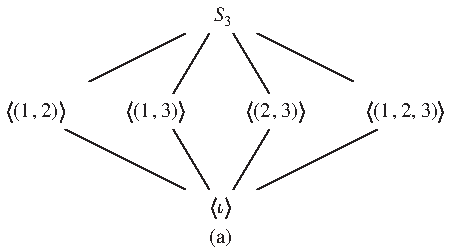
\includegraphics[width=0.616\linewidth,height=.8\textheight,keepaspectratio]{assets/p386_00.pdf}\end{center}
\end{BookFloat}

\begin{BookFloat}{46_galois_theory-p386-1}
\begin{center}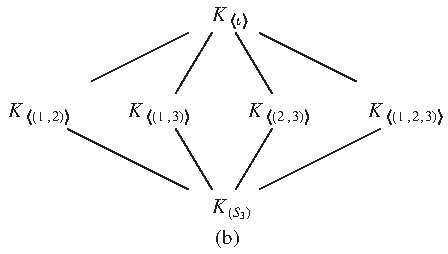
\includegraphics[width=0.614\linewidth,height=.8\textheight,keepaspectratio]{assets/p386_01.pdf}\end{center}
\begin{center}\small\textbf{46.12 Figure}\end{center}
\end{BookFloat}

\begin{center}\begin{adjustbox}{max width=\linewidth}\BookInline{\displaystyle K _ { \langle ( 1 ,\allowbreak  2 ) \rangle } = \mathbb { Q } ( r _ { 3 } ) = \mathbb { Q } \left( \frac { \sqrt [ 3 ] { 2 } } { 2 } \left( - 1 - \sqrt { 3 } i \right) \right)}\end{adjustbox}\end{center}

\begin{center}\begin{adjustbox}{max width=\linewidth}\BookInline{\displaystyle K _ { \langle ( 1 ,\allowbreak  3 ) \rangle } = \mathbb { Q } ( r _ { 2 } ) = \mathbb { Q } \left( \frac { \sqrt [ 3 ] { 2 } } { 2 } \left( - 1 + \sqrt { 3 } i \right) \right)}\end{adjustbox}\end{center}

\begin{center}\begin{adjustbox}{max width=\linewidth}\BookInline{\displaystyle K_{\langle (1,\allowbreak 2,\allowbreak 3)\rangle }= \mathbb{Q}(\sqrt{3}i)}\end{adjustbox}\end{center}

Normal subgroups of \BookInline{G(K/\mathbb{Q})} correspond to subfields of \BookInline{K} that are normal extensions of \BookInline{\mathbb{Q}} by Theorem 46.8. Thus the only intermediate fields of \BookInline{K} that are normal extensions of \BookInline{\mathbb{Q}} are \BookInline{K,\allowbreak \mathbb{Q},\allowbreak } and \BookInline{\mathbb{Q}(\sqrt{3}i)} corresponding to the normal subgroups of \BookInline{S_{3},\allowbreak } namely \BookInline{\{\iota \},\allowbreak S_{3},\allowbreak } and \BookInline{\langle (1,\allowbreak 2,\allowbreak 3)\rangle,\allowbreak } respectively\BookInline{.}\BookEnd{\blacktriangle}

Not every subgroup diagram of a Galois group looks like its own inversion, as we will see in the next section. \BookEnd{\blacksquare}

\end{BookBody}

\BookNarrativefalse

\begin{BookBody}

\BookExerciseTitle{46}

\BookTextHeading{\textbf{Computations}}

\noindent The field \BookInline{K= \mathbb{Q}(\sqrt{2},\allowbreak \sqrt{3},\allowbreak \sqrt{5})} is a finite normal extension of \BookInline{\mathbb{Q}.} It can be shown that \BookInline{[K:\mathbb{Q}]= 8.} In Exercises 1 through 8, compute the indicated numerical quantity. The notation is that of Definition 46.1.

\BookExercise{2.}{\BookInline{|G(K/\mathbb{Q})|}}

\BookExercise{1.}{\BookInline{[K:\mathbb{Q}\sqrt{2}]}}

\BookExercise{4.}{\BookInline{|\lambda (\mathbb{Q}(\sqrt{2},\allowbreak \sqrt{3}))|}}

\BookExercise{3.}{\BookInline{|\lambda (\mathbb{Q})|}}

\BookExercise{6.}{\BookInline{|\lambda (\mathbb{Q}(\sqrt{30}))|}}

\BookExercise{5.}{\BookInline{|\lambda (\mathbb{Q}(\sqrt{6}))|}}

\BookExercise{8.}{\BookInline{|\lambda (K)|}}

\BookExercise{7.}{\BookInline{|\lambda (\mathbb{Q}(\sqrt{2}+ \sqrt{6}))|}}

\end{BookBody}

% Source PDF page 387; original printed page 370
\BookSource{387}{370}
\BookNarrativefalse

\begin{BookBody}

\BookExercise{9.}{Describe the group of the polynomial \BookInline{(x^{4}- 1)\in \mathbb{Q}[x]} over \BookInline{\mathbb{Q}.}}

\BookExercise{10.}{Let \BookInline{G} be the group of the polynomial \BookInline{x^{3}+ 2} over \BookInline{\mathbb{Q}.} Find the order of \BookInline{G} and identify a well-known group that is isomorphic with \BookInline{G.}}

\BookExercise{11.}{Let \BookInline{K} be the splitting field of \BookInline{x^{3}- 5} over \BookInline{\mathbb{Q}.}}

\textbf{a.} Show that \BookInline{K= \mathbb{Q}(\sqrt[3]{5},\allowbreak i\sqrt{3}).}

\textbf{b.} Describe the six elements of \BookInline{G(K/\mathbb{Q})} by giving their values on \BookInline{\sqrt { 5 }} and \BookInline{i\sqrt{3}.}

\BookExercise{c.}{To what group we have seen before is \BookInline{G(K/\mathbb{Q})} isomorphic?}

\BookExercise{d.}{Using the notation given in the answer to part (b) in the back of the text, give the diagrams for the subfields of \BookInline{K} and for the subgroups of \BookInline{G(K/\mathbb{Q}),\allowbreak } indicating corresponding intermediate fields and subgroups, as we did in Example 46.11.}

\BookExercise{12.}{Describe the group of the polynomial \BookInline{(x^{4}- 5x^{2}+ 6)\in \mathbb{Q}[x]} over \BookInline{\mathbb{Q}.}}

\BookExercise{13.}{Describe the group of the polynomial \BookInline{(x^{3}- 1)\in \mathbb{Q}[x]} over \BookInline{\mathbb{Q}.}}

\BookTextHeading{\textbf{Concepts}}

\BookExercise{14.}{Give an example of two normal extensions \BookInline{K_{1}} and \BookInline{K_{2}} of the same field \BookInline{F} such that \BookInline{K_{1}} and \BookInline{K_{2}} are not isomorphic fields but \BookInline{G(K_{1}/F)\simeq G(K_{2}/F).}}

\BookExercise{15.}{Determine whether each of the following is true or false.}

\BookExercise{a.}{Two different subgroups of a Galois group may have the same fixed field.}

\BookExercise{b.}{If \BookInline{F\leq E<L\leq K} are field extensions and \BookInline{K} is a normal extension of \BookInline{F,\allowbreak } then \BookInline{\lambda (E)<\lambda (L).}}

\BookExercise{c.}{If \BookInline{K} is a normal extension of \BookInline{F,\allowbreak } then \BookInline{K} is a normal extension of \BookInline{E,\allowbreak } where \BookInline{F\leq E\leq K.}}

\BookExercise{d.}{If two normal extensions \BookInline{E} and \BookInline{L} of a field \BookInline{F} have isomorphic Galois groups, then \BookInline{[E:F]= [L:F].}}

\BookExercise{e.}{If \BookInline{E} is a normal extension of \BookInline{F} and \BookInline{H} is a normal subgroup of \BookInline{G(E/F),\allowbreak } then \BookInline{E_{H}} is a normal extension of \BookInline{F.}}

\BookExercise{f.}{If \BookInline{E} is any normal simple extension of a field \BookInline{F,\allowbreak } then the Galois group \BookInline{G(E/F)} is a simple group.}

\BookExercise{g.}{No Galois group is simple.}

\BookExercise{h.}{If two intermediate fields \BookInline{E_{1}} and \BookInline{E_{2}} of a normal extension \BookInline{K} over \BookInline{F} have isomorphic groups\BookInline{,\allowbreak \lambda (E_{1})} and \BookInline{\lambda (E_{2}),\allowbreak } then \BookInline{K_{\lambda (E_{1})}} is isomorphic with \BookInline{K_{\lambda (E_{2})}.}}

\BookExercise{i.}{An extension \BookInline{E} of degree 2 over a field \BookInline{F} is always a normal extension of \BookInline{F.}}

\BookExercise{j.}{An extension \BookInline{E} of degree 2 over a field \BookInline{F} is always a normal extension of \BookInline{F} if the characteristic of \BookInline{F} is zero.}

\BookTextHeading{\textbf{Theory}}

\BookExercise{16.}{A normal extension \BookInline{K} of a field \BookInline{F} is\textbf{ abelian over} \BookInline{F} if \BookInline{G(K/F)} is an abelian group. Show that if \BookInline{K} is abelian over \BookInline{F} and \BookInline{F\leq E\leq K,\allowbreak } then \BookInline{K} is abelian over \BookInline{E} and \BookInline{E} is abelian over \BookInline{F.}}

\BookExercise{17.}{Let \BookInline{K} be a normal extension of a field \BookInline{F.} Prove that for every \BookInline{\alpha \in K,\allowbreak } the\textbf{ norm of} \BookInline{\alpha } \textbf{over} \BookInline{F,\allowbreak } given by}

\begin{center}\begin{adjustbox}{max width=\linewidth}\BookInline{\displaystyle N_{K/F}(\alpha )= _{\sigma \in G}\prod _{(K/F)}\sigma (\alpha ),\allowbreak }\end{adjustbox}\end{center}

\noindent and the\textbf{ trace of} \BookInline{\alpha } \textbf{over} \BookInline{F,\allowbreak } given by

\begin{center}\begin{adjustbox}{max width=\linewidth}\BookInline{\displaystyle Tr_{K/F}(\alpha )= _{\sigma \in G}\sum _{(K/F)}\sigma (\alpha ),\allowbreak }\end{adjustbox}\end{center}

\noindent are elements of \BookInline{F.}

\BookExercise{18.}{Consider \BookInline{K= \mathbb{Q}(\sqrt{2},\allowbreak \sqrt{3}).} Referring to Exercise 17, compute each of the following (see Table 43.5).}

\textbf{a.} \BookInline{N _ { K / \mathbb { Q } } ( { \sqrt { 2 } } )}

\textbf{b}\BookInline{.N_{K/\mathbb{Q}}(\sqrt{2}+ \sqrt{3})}

\textbf{c.} \BookInline{N _ { K / \mathbb { Q } } ( { \sqrt { 6 } } )}

\BookExercise{d.}{\BookInline{N_{K/\mathbb{Q}}(2)}}

\textbf{e.} \BookInline{T r _ { K / \mathbb { Q } } ( { \sqrt { 2 } } )} \textbf{f.}\textit{ Tr}\BookInline{K/\mathbb{Q}(\sqrt 2+ \sqrt 3)}

\textbf{g.}\textit{ Tr}\BookInline{K/\mathbb{Q}(\sqrt 6)}

\BookExercise{h.}{\textit{ Tr}\BookInline{K/\mathbb{Q}(2)}}

\end{BookBody}

% Source PDF page 388; original printed page 371
\BookSource{388}{371}
\BookNarrativefalse

\begin{BookBody}

\BookExercise{19.}{Let \BookInline{K= F(\alpha )} be a normal extension of \BookInline{F.} Let}

\begin{center}\begin{adjustbox}{max width=\linewidth}\BookInline{\displaystyle \;\text{irr}\;(\alpha ,\allowbreak F)= x^{n}+ a_{n- 1}x^{n- 1}+ \cdots + a_{1}x+ a_{0}.}\end{adjustbox}\end{center}

Referring to Exercise 17, show that

\BookExercise{a.}{\textbf{a}\BookInline{.N_{K/F}(\alpha )= (- 1)^{n}a_{0},\allowbreak }}

\begin{center}\begin{adjustbox}{max width=\linewidth}\BookInline{\displaystyle \mathrm{b}.Tr_{K/F}(\alpha )= - a_{n- 1}.}\end{adjustbox}\end{center}

\BookExercise{20.}{Let \BookInline{f(x)\in F[x]} be a polynomial of degree \BookInline{n} such that each irreducible factor is separable over \BookInline{F.} Show that the order of the group of \BookInline{f(x)} over \BookInline{F} divides \BookInline{n}!.}

\BookExercise{21.}{Let \BookInline{f(x)\in F[x]} be a polynomial such that every irreducible factor of \BookInline{f(x)} is a separable polynomial over \BookInline{F.} Show that the group of \BookInline{f(x)} over \BookInline{F} can be viewed in a natural way as a group of permutations of the zeros of \BookInline{f(x)} in \BookInline{F.}}

\BookExercise{22.}{Let \BookInline{F} be a field and let \BookInline{\zeta } be a primitive \BookInline{n}th root of unity in \BookInline{F,\allowbreak } where the characteristic of \BookInline{F} is 0.}

\BookExercise{a.}{Show that \BookInline{F(\zeta )} is a normal extension of \BookInline{F.}}

\BookExercise{b.}{Show that \BookInline{G(F(\zeta )/F)} is abelian. [\textit{Hint:} Every \BookInline{\sigma \in G(F(\zeta )/F)} maps \BookInline{\zeta } onto some \BookInline{\zeta ^{r}} and is completely determined by this value \BookInline{r.]}}

\BookExercise{23.}{A normal extension \BookInline{K} of a field \BookInline{F} is\textbf{ cyclic over} \BookInline{F} if \BookInline{G(K/F)} is a cyclic group.}

\BookExercise{a.}{Show that if \BookInline{K} is cyclic over \BookInline{F} and \BookInline{F\leq E\leq K,\allowbreak } then \BookInline{E} is cyclic over \BookInline{F} and \BookInline{K} is cyclic over \BookInline{E.}}

\BookExercise{b.}{Show that if \BookInline{K} is cyclic over \BookInline{F,\allowbreak } then there exists exactly one field \BookInline{E,\allowbreak F\leq E\leq K,\allowbreak } of degree \BookInline{d} over \BookInline{F} for each divisor \BookInline{d} of \BookInline{[K:F].}}

\BookExercise{24.}{Let \BookInline{K} be a normal extension of \BookInline{F.}}

\BookExercise{a.}{For \BookInline{\alpha \in K,\allowbreak } show that}

\begin{center}\begin{adjustbox}{max width=\linewidth}\BookInline{\displaystyle f(x)= _{\sigma \in G}\prod _{(K/F)}(x- \sigma (\alpha ))}\end{adjustbox}\end{center}

is in \BookInline{F[x].}

\BookExercise{b.}{Referring to part (a), show that \BookInline{f(x)} is a power of irr\BookInline{(\alpha,\allowbreak F),\allowbreak } and \BookInline{f(x)= } irr\BookInline{(\alpha,\allowbreak F)} if and only if \BookInline{K= F(\alpha ).}}

\BookExercise{25.}{Let \BookInline{K} be a normal extension of the field \BookInline{F.} If \BookInline{E} and \BookInline{L} are both intermediate fields of the extension, the\textbf{ join}, \BookInline{E\vee L,\allowbreak } is the intersection of all intermediate fields of the extension that contain both \BookInline{E} and \BookInline{L.} See Figure 46.13. Describe \BookInline{G(K/(E\vee L))} in terms of \BookInline{G(K/E)} and \BookInline{G(K/L).}}

\BookExercise{26.}{With reference to the situation in Exercise 25, describe \BookInline{G(K/(E\cap L))} in terms of \BookInline{G(K/E)} and \BookInline{G(K/L).}}

\begin{BookFloat}{46_galois_theory-p388-20}
\begin{center}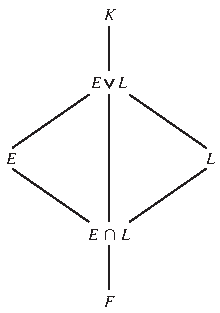
\includegraphics[width=0.301\linewidth,height=.8\textheight,keepaspectratio]{assets/p388_20.pdf}\end{center}
\begin{center}\small\textbf{46.13 Figure}\end{center}
\end{BookFloat}

\end{BookBody}
\ifdefined\BookMaster\let\BookFinish\relax\else\def\BookFinish{\end{document}}\fi\BookFinish

\clearpage
% !TeX program = xelatex
\ifdefined\BookMaster\else
\documentclass[11pt,oneside]{article}
% !TeX program = xelatex
\usepackage[b5paper,left=22mm,right=22mm,top=20mm,bottom=22mm,footskip=11mm]{geometry}
\usepackage{fontspec}
\setmainfont{TeX Gyre Termes}
\setsansfont{TeX Gyre Heros}
\usepackage{amsmath,amssymb,mathtools,amsthm}
\renewcommand{\cdots}{\mathinner{\cdotp\cdotp\cdotp}}
\usepackage{graphicx,adjustbox,array,booktabs,longtable,multirow,enumitem,changepage,needspace}
\usepackage[table]{xcolor}
\usepackage{fancyhdr}
\raggedbottom
\interfootnotelinepenalty=10000
\newcommand{\BookFootnote}[2]{\begingroup\renewcommand{\thefootnote}{\fnsymbol{footnote}}\footnote[#1]{#2}\endgroup}
\newcommand{\BookFootnoteMark}[1]{\begingroup\renewcommand{\thefootnote}{\fnsymbol{footnote}}\footnotemark[#1]\endgroup}
\newcommand{\BookFootnoteText}[2]{\begingroup\renewcommand{\thefootnote}{\fnsymbol{footnote}}\footnotetext[#1]{#2}\endgroup}
\newenvironment{BookFloat}[1]{\par\addvspace{.6\baselineskip}\noindent\def\BookFloatID{#1}\begin{minipage}{\linewidth}\phantomsection\label{bookfloat:#1:start}}{\phantomsection\label{bookfloat:\BookFloatID:end}\end{minipage}\par\addvspace{.6\baselineskip}}

\usepackage[unicode,hidelinks]{hyperref}
\pagestyle{fancy}
\fancyhf{}
\newcommand{\BookFooter}{}
\fancyfoot[L]{\parbox[b]{\dimexpr\textwidth-15mm}{\footnotesize\BookFooter}}
\fancyfoot[R]{\footnotesize\thepage}
\renewcommand{\headrulewidth}{0pt}
\renewcommand{\footrulewidth}{0pt}
\setlength{\parindent}{0pt}
\setlength{\parskip}{0.2em}
\setlength{\emergencystretch}{3em}
\setlist{nosep,leftmargin=1.7em,labelsep=.65em}
\newif\ifBookNarrative
\BookNarrativetrue
\newenvironment{BookBody}{\setlength{\parindent}{0pt}}{}
\newcommand{\BookStatement}[1]{\par\addvspace{.6\baselineskip}\noindent #1\enspace\ignorespaces}
\newcommand{\BookLabel}[1]{\par\addvspace{.6\baselineskip}\needspace{3\baselineskip}\noindent\textbf{#1}\quad\ignorespaces}
\newcommand{\BookHeading}[1]{\par\addvspace{\baselineskip}\needspace{4\baselineskip}\noindent{\large\bfseries #1}\par\medskip}
\newcommand{\BookSubheading}[1]{\par\addvspace{.7\baselineskip}\needspace{3\baselineskip}\noindent{\bfseries #1}\par\smallskip}
\newcommand{\BookTextHeading}[1]{\par\addvspace{.7\baselineskip}\needspace{3\baselineskip}\noindent #1\par\smallskip}
\newcommand{\BookSectionTitle}[2]{\par\addvspace{1.2\baselineskip}\needspace{5\baselineskip}\noindent\colorbox{gray!25}{\sffamily\bfseries\small SECTION #1}\quad{\large\bfseries #2}\par\medskip}
\newcommand{\BookExerciseTitle}[1]{\par\addvspace{\baselineskip}\needspace{4\baselineskip}\noindent{\color{gray}\rule{1.5mm}{1.5mm}}\enspace{\large\bfseries Exercises #1}\par\medskip}
\newcommand{\BookBullet}[1]{\begin{list}{\textbullet}{\setlength{\leftmargin}{1.7em}\setlength{\labelwidth}{1em}\setlength{\labelsep}{.7em}\setlength{\topsep}{0pt}\setlength{\parsep}{0pt}\setlength{\itemsep}{0pt}}\item #1\end{list}}
\newcommand{\BookExercise}[2]{\begin{list}{\textbf{#1}}{\setlength{\leftmargin}{2.2em}\setlength{\labelwidth}{1.5em}\setlength{\labelsep}{.7em}\setlength{\topsep}{.15em}\setlength{\parsep}{0pt}\setlength{\itemsep}{0pt}}\item #2\end{list}}
\newcommand{\BookEnd}[1]{\unskip\nobreak\hfill\ensuremath{#1}}
\newcommand{\BookSource}[2]{\phantomsection\label{sourcepage:#1}} % Source-page anchors, retained through reflow.
\usepackage{multicol}
\usepackage{tikz}
\newcommand{\BookPartEntry}[2]{\par\noindent\makebox[17mm][l]{\bfseries Section #1}#2\par}
\newcommand{\BookPartTitle}[3]{\par\bigskip\noindent\begin{tikzpicture}\node[anchor=north west,inner sep=0pt,outer sep=0pt] (bookpart) at (0,0) {\begin{minipage}{\dimexpr\linewidth-.5pt}\hspace*{26mm}\begin{minipage}[t]{\dimexpr\linewidth-26mm}\begin{adjustbox}{max width=\linewidth}{\fontsize{20}{24}\selectfont\bfseries #2}\end{adjustbox}\par\vspace{6mm}\hrule\vspace{6mm}{\sffamily\footnotesize\setlength{\parskip}{.3em}#3}\vspace{3mm}\end{minipage}\end{minipage}};\path[shade,top color=gray!60,bottom color=white] (0,0) rectangle ([xshift=24mm]bookpart.south west);\node[anchor=north,font=\sffamily\bfseries\small] at (12mm,-2mm) {PART};\node[anchor=north,font=\sffamily\bfseries\Huge] at (12mm,-7mm) {#1};\end{tikzpicture}\par\bigskip}
\newsavebox{\BookMathBox}
\makeatletter
\newcommand{\BookInline}[1]{\leavevmode\hskip0pt\relax\begingroup\in@{\begin}{#1}\ifin@\sbox{\BookMathBox}{\(#1\)}\ifdim\wd\BookMathBox>\dimexpr\linewidth-1em\relax\resizebox{\dimexpr\linewidth-1em\relax}{!}{\usebox{\BookMathBox}}\else\(#1\)\fi\else\in@{\left}{#1}\ifin@\sbox{\BookMathBox}{\(#1\)}\ifdim\wd\BookMathBox>\dimexpr\linewidth-1em\relax\resizebox{\dimexpr\linewidth-1em\relax}{!}{\usebox{\BookMathBox}}\else\(#1\)\fi\else\(#1\)\fi\fi\endgroup\hskip0pt\relax}
\makeatother
\DeclareMathOperator{\Aut}{Aut}
\DeclareMathOperator{\End}{End}
\DeclareMathOperator{\Hom}{Hom}
\DeclareMathOperator{\GF}{GF}
\DeclareMathOperator{\irr}{irr}
\DeclareMathOperator{\lt}{lt}
\DeclareMathOperator{\lp}{lp}
\providecommand{\textcircled}[1]{\textnormal{(#1)}}

\begin{document}
\fi
\renewcommand{\BookFooter}{Section 47 Illustrations of Galois Theory}
\pdfbookmark[0]{Section 47 Illustrations of Galois Theory}{47_illustrations_of_galois_theory}
\ifdefined\BookMaster\else\setcounter{page}{372}\fi
% Source PDF page 389; original printed page 372
\BookSource{389}{372}
\BookNarrativetrue

\begin{BookBody}

\BookSectionTitle{47}{Illustrations of Galois Theory}

\BookTextHeading{\textbf{Symmetric Functions}  }

\noindent Let \BookInline{F} be a field of characteristic zero, and let \BookInline{y_{1},\allowbreak \cdots,\allowbreak y_{n}} be indeterminates. There are some natural automorphisms of \BookInline{F(y_{1},\allowbreak \cdots,\allowbreak y_{n})} leaving \BookInline{F} fixed, namely, those defined by permutations of \BookInline{\{y_{1},\allowbreak \cdots,\allowbreak y_{n}\}.} To be more explicit, let \BookInline{\sigma } be a permutation of \BookInline{\{1,\allowbreak \cdots,\allowbreak n\},\allowbreak } that is\BookInline{,\allowbreak \sigma \in S_{n}.} Then \BookInline{\sigma } gives rise to a natural map \BookInline{\sigma:F(y_{1},\allowbreak \cdots,\allowbreak y_{n})\to F(y_{1},\allowbreak \cdots,\allowbreak y_{n})} given by

\begin{center}\begin{adjustbox}{max width=\linewidth}\BookInline{\displaystyle \overline { { \sigma } } \left( \frac { f ( y _ { 1 } ,\allowbreak  \cdots ,\allowbreak  y _ { n } ) } { g ( y _ { 1 } ,\allowbreak  \cdots ,\allowbreak  y _ { n } ) } \right) = \frac { f ( y _ { \sigma ( 1 ) } ,\allowbreak  \cdots ,\allowbreak  y _ { \sigma ( n ) } ) } { g ( y _ { \sigma ( 1 ) } ,\allowbreak  \cdots ,\allowbreak  y _ { \sigma ( n ) } ) }}\end{adjustbox}\end{center}

\noindent for \BookInline{f(y_{1},\allowbreak \cdots,\allowbreak y_{n}),\allowbreak g(y_{1},\allowbreak \cdots,\allowbreak y_{n})\in F[y_{1},\allowbreak \cdots,\allowbreak y_{n}],\allowbreak } with \BookInline{g(y_{1},\allowbreak \cdots,\allowbreak y_{n})\neq 0.} It is immediate that \BookInline{\overline{\sigma }} is an automorphism of \BookInline{F(y_{1},\allowbreak \cdots,\allowbreak y_{n})} leaving \BookInline{F} fixed. The elements of \BookInline{F(y_{1},\allowbreak \cdots,\allowbreak y_{n})} left fixed by\textit{ all} \BookInline{\overline{\sigma },\allowbreak } for all \BookInline{\sigma \in S_{n},\allowbreak } are those rational functions that are \textit{symmetric} in the indeterminates \BookInline{y_{1},\allowbreak \cdots,\allowbreak y_{n}.}

\BookLabel{47.1 Definition} An element of the field \BookInline{F(y_{1},\allowbreak \cdots,\allowbreak y_{n})} is a\textbf{ symmetric function in} \BookInline{y_{1},\allowbreak \cdots,\allowbreak y_{n}} \textbf{over} \BookInline{F,\allowbreak } if it is fixed by all permutations of \BookInline{y_{1},\allowbreak \cdots,\allowbreak y_{n},\allowbreak } in the sense just explained\BookInline{.}\BookEnd{\blacksquare}

Let \BookInline{\overline{S_{n}}} be the group of all the automorphisms \BookInline{\overline{\sigma }} for \BookInline{\sigma \in S_{n}.} Observe that \BookInline{\overline{S_{n}}} is naturally isomorphic to \BookInline{S_{n}.} Let \BookInline{K} be the subfield of \BookInline{F(y_{1},\allowbreak \cdots,\allowbreak y_{n}),\allowbreak } which is the fixed field of \BookInline{\overline{S_{n}}.} Consider the polynomial

\begin{center}\begin{adjustbox}{max width=\linewidth}\BookInline{\displaystyle f(x)= \prod _{i= 1}^{n}(x- y_{i});}\end{adjustbox}\end{center}

\noindent this polynomial \BookInline{f(x)\in (F(y_{1},\allowbreak \cdots,\allowbreak y_{n}))[x]} is a\textbf{ general polynomial of degree} \BookInline{n.} Let \BookInline{\overline{\sigma _{x}}} be the polynomial extension of \BookInline{\overline{\sigma },\allowbreak } as defined in Definition 44.4, to \BookInline{(F(y_{1},\allowbreak \cdots,\allowbreak y_{n}))[x],\allowbreak } where \BookInline{\overline{\sigma _{x}}(x)= x.} Now \BookInline{f(x)} is fixed by each map \BookInline{\overline{\sigma _{x}}} for \BookInline{\sigma \in S_{n};} that is,

\begin{center}\begin{adjustbox}{max width=\linewidth}\BookInline{\displaystyle \prod _{i= 1}^{n}(x- y_{i})= \prod _{i= 1}^{n}(x- y_{\sigma (i)}).}\end{adjustbox}\end{center}

\noindent Thus the coefficients of \BookInline{f(x)} are in \BookInline{K;} they are, except for sign, the\textit{ elementary symmetric} \textit{functions} in \BookInline{y_{1},\allowbreak \cdots,\allowbreak y_{n}.} As illustration, note that the constant term of \BookInline{f(x)} is

\begin{center}\begin{adjustbox}{max width=\linewidth}\BookInline{\displaystyle (- 1)^{n}y_{1}y_{2}\cdots y_{n},\allowbreak }\end{adjustbox}\end{center}

\noindent the coefficient of \BookInline{x^{n- 1}} is \BookInline{- (y_{1}+ y_{2}+ \cdots + y_{n}),\allowbreak } and so on. These are symmetric functions in \BookInline{y_{1},\allowbreak \cdots,\allowbreak y_{n}.}

The first elementary symmetric function in \BookInline{y_{1},\allowbreak \cdots,\allowbreak y_{n}} is

\begin{center}\begin{adjustbox}{max width=\linewidth}\BookInline{\displaystyle s_{1}= y_{1}+ y_{2}+ \cdots + y_{n},\allowbreak }\end{adjustbox}\end{center}

\noindent the second is \BookInline{s_{2}= y_{1}y_{2}+ y_{1}y_{3}+ \cdots + y_{n- 1}y_{n},\allowbreak } and so on, and the \BookInline{n}th is \BookInline{s_{n}= y_{1}y_{2}\cdots y_{n}.} Consider the field \BookInline{E= F(s_{1},\allowbreak \cdots,\allowbreak s_{n}).} Of course\BookInline{,\allowbreak E\leq K,\allowbreak } where \BookInline{K} is the field of all symmetric functions in \BookInline{y_{1},\allowbreak \cdots,\allowbreak y_{n}} over \BookInline{F.} Since the characteristic of \BookInline{E} is zero, the extension \BookInline{K} over \BookInline{E} is a separable extension. Thus \BookInline{F(y_{1},\allowbreak \cdots,\allowbreak y_{n})} is a finite normal extension of \BookInline{E,\allowbreak } namely, the splitting field of

\begin{center}\begin{adjustbox}{max width=\linewidth}\BookInline{\displaystyle f(x)= \prod _{i= 1}^{n}(x- y_{i})}\end{adjustbox}\end{center}

\noindent over \BookInline{E.} Since the degree of \BookInline{f(x)} is \BookInline{n,\allowbreak } we have at once that

\begin{center}\begin{adjustbox}{max width=\linewidth}\BookInline{\displaystyle [F(y_{1},\allowbreak \cdots ,\allowbreak y_{n}):E]\leq n!}\end{adjustbox}\end{center}

\end{BookBody}

% Source PDF page 390; original printed page 373
\BookSource{390}{373}
\BookNarrativetrue

\begin{BookBody}

\noindent (see Exercise 19, Section 44). However, since \BookInline{K} is the fixed field of \BookInline{\overline{S_{n}}} and

\begin{center}\begin{adjustbox}{max width=\linewidth}\BookInline{\displaystyle |\overline{S_{n}}|= |S_{n}|= n!,\allowbreak }\end{adjustbox}\end{center}

\noindent we have also

\begin{center}\begin{adjustbox}{max width=\linewidth}\BookInline{\displaystyle n!= [F(y_{1},\allowbreak \cdots ,\allowbreak y_{n}):K].}\end{adjustbox}\end{center}

\noindent Therefore,

\begin{center}\begin{adjustbox}{max width=\linewidth}\BookInline{\displaystyle n!= [F(y_{1},\allowbreak \cdots ,\allowbreak y_{n}):K]\leq [F(y_{1},\allowbreak \cdots ,\allowbreak y_{n}):E]\leq n!,\allowbreak }\end{adjustbox}\end{center}

\noindent so

\begin{center}\begin{adjustbox}{max width=\linewidth}\BookInline{\displaystyle K= E.}\end{adjustbox}\end{center}

\noindent The full Galois group of \BookInline{F(y_{1},\allowbreak \cdots,\allowbreak y_{n})} over \BookInline{E} is therefore \BookInline{\overline{S_{n}}.} The fact that \BookInline{K= E} shows that every symmetric function can be expressed as a rational function of the elementary symmetric functions \BookInline{s_{1},\allowbreak \cdots,\allowbreak s_{n}.} We summarize these results in a theorem.

\BookLabel{47.2 Theorem} Let \BookInline{F} be a field with characteristic zero. Let \BookInline{s_{1},\allowbreak \cdots,\allowbreak s_{n}} be the elementary symmetric functions in the indeterminates \BookInline{y_{1},\allowbreak \cdots,\allowbreak y_{n}.} Then every symmetric function of \BookInline{y_{1},\allowbreak \cdots,\allowbreak y_{n}} over \BookInline{F} is a rational function of the elementary symmetric functions. Also\BookInline{,\allowbreak F(y_{1},\allowbreak \cdots,\allowbreak y_{n})} is a finite normal extension of degree \BookInline{n!} of \BookInline{F(s_{1},\allowbreak \cdots,\allowbreak s_{n}),\allowbreak } and the Galois group of this extension is naturally isomorphic to \BookInline{S_{n}.}

In view of Cayley’s Theorem 8.11, it can be deduced from Theorem 47.2 that any finite group can occur as a Galois group (up to isomorphism). (See Exercise 11.)

The proof of Theorem 47.2 only uses the fact that the characteristic of \BookInline{F} is zero to conclude that the extension \BookInline{F(y_{1},\allowbreak y_{2},\allowbreak...,\allowbreak y_{n})} over \BookInline{E} is a separable extension. With a bit more work, the proof can be modified to allow \BookInline{F} to be an arbitrary field.

\BookTextHeading{\textbf{Examples}}

\noindent Let us give our promised example of a finite normal extension having a Galois group whose subgroup diagram does not look like its own inversion.

\BookLabel{47.3 Example} Consider the splitting field in \BookInline{\mathbb{C}} of \BookInline{x^{4}- 2} over \BookInline{\mathbb{Q}.} Now \BookInline{x^{4}- 2} is irreducible over \BookInline{\mathbb{Q},\allowbreak } by Eisenstein’s criterion, with \BookInline{p= 2.} Let \BookInline{\alpha = \sqrt [ 4 ] { 2 }} be the real positive zero of \BookInline{x^{4}- 2.} Then the four zeros of \BookInline{x^{4}- 2} in \BookInline{\mathbb{C}} are \BookInline{\alpha,\allowbreak - \alpha,\allowbreak i\alpha,\allowbreak } and \BookInline{- i\alpha,\allowbreak } where \BookInline{i} is the usual zero of \BookInline{x^{2}+ 1} in \BookInline{\mathbb{C}.} The splitting field \BookInline{K} of \BookInline{x^{4}- 2} over \BookInline{\mathbb{Q}} thus contains \BookInline{(i\alpha )/\alpha = i.} Since \BookInline{\alpha } is a real number\BookInline{,\allowbreak \mathbb{Q}(\alpha )<\mathbb{R},\allowbreak } so \BookInline{\mathbb{Q}(\alpha )\neq K.} However, since \BookInline{\mathbb{Q}(\alpha,\allowbreak i)} contains all zeros of \BookInline{x^{4}- 2,\allowbreak } we see that \BookInline{\mathbb{Q}(\alpha,\allowbreak i)= K.} Letting \BookInline{E= \mathbb{Q}(\alpha ),\allowbreak } we have the diagram in Fig. 47.4.

\begin{BookFloat}{47_illustrations_of_galois_theory-p390-15}
\begin{center}\begin{tikzpicture}
\node[anchor=west] (K) at (0,3) {$K=\mathbb{Q}(\alpha,i)$};
\node[anchor=west] (E) at (0,1.5) {$E=\mathbb{Q}(\alpha)$};
\node[anchor=west] (Q) at (0,0) {$\mathbb{Q}$};
\draw (0.1,2.75)--(0.1,1.75);
\draw (0.1,1.25)--(0.1,0.25);
\end{tikzpicture}\end{center}
\begin{center}\small \textbf{47.4 Figure}\end{center}
\end{BookFloat}

Now \BookInline{\{1,\allowbreak \alpha,\allowbreak \alpha ^{2},\allowbreak \alpha ^{3}\}} is a basis for \BookInline{E} over \BookInline{\mathbb{Q},\allowbreak } and \BookInline{\{1,\allowbreak i\}} is a basis for \BookInline{K} over \BookInline{E.} Thus

\begin{center}\begin{adjustbox}{max width=\linewidth}\BookInline{\displaystyle \{1,\allowbreak \alpha ,\allowbreak \alpha ^{2},\allowbreak \alpha ^{3},\allowbreak i,\allowbreak i\alpha ,\allowbreak i\alpha ^{2},\allowbreak i\alpha ^{3}\}}\end{adjustbox}\end{center}

\noindent is a basis for \BookInline{K} over \BookInline{\mathbb{Q}.} Since \BookInline{[K:\mathbb{Q}]= 8,\allowbreak } we must have \BookInline{|G(K/\mathbb{Q})|= 8,\allowbreak } so we need to find eight automorphisms of \BookInline{K} leaving \BookInline{\mathbb{Q}} fixed. We know that any such automorphism \BookInline{\sigma } is completely determined by its values on elements of the basis \BookInline{\{1,\allowbreak \alpha,\allowbreak \alpha ^{2},\allowbreak \alpha ^{3},\allowbreak i,\allowbreak i\alpha,\allowbreak i\alpha ^{2},\allowbreak } \BookInline{i\alpha ^{3}\},\allowbreak } and these values are in turn determined by \BookInline{\sigma (\alpha )} and \BookInline{\sigma (i).} But \BookInline{\sigma (\alpha )} must always be a conjugate of \BookInline{\alpha } over \BookInline{\mathbb{Q},\allowbreak } that is, one of the four zeros of irr\BookInline{(\alpha,\allowbreak \mathbb{Q})= x^{4}- 2.} Likewise\BookInline{,\allowbreak \sigma (i)} must be a zero of irr\BookInline{(i,\allowbreak \mathbb{Q})= x^{2}+ 1.} Thus the four possibilities for \BookInline{\sigma (\alpha ),\allowbreak } combined with the two possibilities for \BookInline{\sigma (i),\allowbreak } must give all eight automorphisms. We let \BookInline{\rho \in G(K/\mathbb{Q})} be the automorphism with \BookInline{\rho (\alpha )= i\alpha } and \BookInline{\rho (i)= i;} and we let \BookInline{\mu \in G(K/\mathbb{Q})} be the automorphism with \BookInline{\mu (\alpha )= \alpha } and \BookInline{\mu (i)= - i.} We have

\begin{center}\begin{adjustbox}{max width=\linewidth}\BookInline{\displaystyle \rho ^{2}(\alpha )= \rho (\rho (\alpha ))= \rho (i\alpha )= i(i\alpha )= - \alpha ,\allowbreak }\end{adjustbox}\end{center}

\begin{center}\begin{adjustbox}{max width=\linewidth}\BookInline{\displaystyle \rho ^{2}(i)= \rho (\rho (i))= \rho (i)= i.}\end{adjustbox}\end{center}

\end{BookBody}

% Source PDF page 391; original printed page 374
\BookSource{391}{374}
\BookNarrativetrue

\begin{BookBody}

\begin{BookFloat}{47_illustrations_of_galois_theory-p391-0}
\begin{center}\small\textbf{47.5 Table}\end{center}
\begin{center}\begin{adjustbox}{max width=\linewidth}
\renewcommand{\arraystretch}{1.2}\setlength{\tabcolsep}{5pt}
\begin{tabular}{c|c|c|c|c|c|c|c|c}
 & \BookInline{\iota } & \BookInline{\rho } & \BookInline{\rho ^{2}} & \BookInline{\rho ^{3}} & \BookInline{\mu } & \BookInline{\mu \rho } & \BookInline{\mu \rho ^{2}} & \BookInline{\mu \rho ^{3}}\\\hline
\BookInline{\alpha \to } & \BookInline{\alpha } & \BookInline{i\alpha } & \BookInline{- \alpha } & \BookInline{- i\alpha } & \BookInline{\alpha } & \BookInline{- i\alpha } & \BookInline{- \alpha } & \BookInline{i\alpha }\\\hline
\BookInline{i\to } & \BookInline{i} & \BookInline{i} & \BookInline{i} & \BookInline{i} & \BookInline{- i} & \BookInline{- i} & \BookInline{- i} & \BookInline{- i}\\
\end{tabular}
\end{adjustbox}\end{center}
\end{BookFloat}

\noindent Similarly, we have

\begin{center}\begin{adjustbox}{max width=\linewidth}\BookInline{\displaystyle \begin{aligned}\mu \rho (\alpha )&= \mu (\rho (\alpha ))= \mu (i\alpha )= - i\alpha ,\allowbreak  \\ \mu \rho (i)&= \mu (\rho (i))= \mu (i)= - i.\end{aligned}}\end{adjustbox}\end{center}

Table 47.5 shows the results of similar computations for \BookInline{\iota,\allowbreak \rho,\allowbreak \rho ^{2},\allowbreak \rho ^{3},\allowbreak \mu,\allowbreak \mu \rho,\allowbreak \mu \rho ^{2},\allowbreak } and \BookInline{\mu \rho ^{3}.} These automorphisms account for all eight of the elements of \BookInline{G(K/\mathbb{Q}).} The table looks remarkably like the dihedral group \BookInline{D_{4}.} To verify that \BookInline{G(K/\mathbb{Q})} is isomorphic with \BookInline{D_{4}} we check the relations \BookInline{\mu ^{2}= \iota,\allowbreak \rho ^{4}= \iota,\allowbreak } and \BookInline{\rho \mu = \mu \rho ^{3}} by evaluating each at \BookInline{\alpha } and \BookInline{i.}

\begin{center}\begin{adjustbox}{max width=\linewidth}\BookInline{\displaystyle \begin{aligned}\mu ^{2}(\alpha )&= \mu (\alpha )= \alpha ,\allowbreak  \\ \mu ^{2}(i)&= \mu (- i)= i,\allowbreak \end{aligned}}\end{adjustbox}\end{center}

\begin{center}\begin{adjustbox}{max width=\linewidth}\BookInline{\displaystyle \begin{aligned}\rho ^{4}(\alpha )&= \rho (\rho ^{3}(\alpha ))= \rho (- i\alpha )= - i^{2}\alpha = \alpha ,\allowbreak  \\ \rho ^{4}(i)&= \rho (\rho ^{3}(i))= \rho (i)= i,\allowbreak \end{aligned}}\end{adjustbox}\end{center}

\begin{center}\begin{adjustbox}{max width=\linewidth}\BookInline{\displaystyle \begin{aligned}\rho \mu (\alpha )&= \rho (\alpha )= i\alpha = \mu \rho ^{3}(\alpha ),\allowbreak  \\ \rho \mu (i)&= \rho (- i)= - i= \mu \rho ^{3}(i).\end{aligned}}\end{adjustbox}\end{center}

The subgroup diagram for the dihedral group is given in Figure 47.6 (a) with the corresponding subfield diagram in Figure 47.6 (b). This provides a good illustration of how one diagram is the inversion of the other.

The determination of the fixed fields \BookInline{K_{H_{i}}} sometimes requires a bit of ingenuity. Let’s illustrate. To find \BookInline{K_{H_{2}}}, we merely have to find an extension of \BookInline{\mathbb{Q}} of degree 2 fixed by \BookInline{\{\iota,\allowbreak \rho,\allowbreak \rho ^{2},\allowbreak \rho ^{3}\}.} Since all \BookInline{\rho ^{j}} leave \BookInline{i} fixed\BookInline{,\allowbreak \mathbb{Q}(i)} is the field we are after. To find \BookInline{K_{H_{4}},\allowbreak } we have to find an extension of \BookInline{\mathbb{Q}} of degree 4 fixed by \BookInline{\iota } and \BookInline{\mu.} Since \BookInline{\mu } leaves \BookInline{\alpha } fixed and \BookInline{\alpha } is a zero of irr\BookInline{(\alpha,\allowbreak \mathbb{Q})= x^{4}- 2,\allowbreak } we see that \BookInline{\mathbb{Q}(\alpha )} is of degree 4 over \BookInline{\mathbb{Q}} and is fixed by \BookInline{\{\iota,\allowbreak \mu \}.} By\textit{ Galois theory, it is the only such} \BookInline{\text{fi}eld.} Here we are using strongly the one-to-one correspondence given by the Galois theory. If we find one field that fits the bill, it is the one we are after. Finding \BookInline{K_{H_{7}}} requires more ingenuity. Since \BookInline{H_{7}} is a group, for any \BookInline{\beta \in K,\allowbreak \iota (\beta )+ \mu \rho ^{3}(\beta )} is fixed by \BookInline{\iota } and \BookInline{\mu \rho ^{3},\allowbreak } the elements of \BookInline{H_{7}.} Letting \BookInline{\beta = \alpha } we see that \BookInline{\iota (\alpha )+ \mu \rho ^{3}(\alpha )= \alpha + i\alpha } is fixed by \BookInline{H_{7}.} By checking all eight automorphisms in Table 47.5, we see that only \BookInline{\iota } and \BookInline{\mu \rho ^{3}} fix \BookInline{\alpha + i\alpha.} Thus by the one-to-one correspondence, we must have

\begin{center}\begin{adjustbox}{max width=\linewidth}\BookInline{\displaystyle \mathbb { Q } ( \alpha + i \alpha ) = \mathbb { Q } ( { \sqrt [ 4 ] { 2 } } + i { \sqrt [ 4 ] { 2 } } ) = K _ { H _ { 7 } } .}\end{adjustbox}\end{center}

Suppose we wish to find irr\BookInline{(\alpha + i\alpha,\allowbreak \mathbb{Q}).} If \BookInline{\gamma = \alpha + i\alpha,\allowbreak } then for every conjugate of \BookInline{\gamma } over \BookInline{\mathbb{Q},\allowbreak } there exists an automorphism of \BookInline{K} mapping \BookInline{\gamma } into that conjugate. Thus we need only compute the various different values \BookInline{\sigma (\gamma )} for \BookInline{\sigma \in G(K/\mathbb{Q})} to find the other zeros of irr\BookInline{(\gamma,\allowbreak \mathbb{Q}).} Every element in \BookInline{D_{4}} can be written in the form \BookInline{\rho ^{i}(\mu \rho ^{3})^{j}} where \BookInline{0\leq i\leq 3} and \BookInline{j} is either 0 or 1. But \BookInline{\mu \rho ^{3}(\alpha + i\alpha )= \alpha + i\alpha,\allowbreak } so to compute the conjugates of \BookInline{\alpha + i\alpha } we only need to compute \BookInline{\iota (\alpha + i\alpha ),\allowbreak \rho (\alpha + i\alpha ),\allowbreak \rho ^{2}(\alpha + i\alpha ),\allowbreak } and \BookInline{\rho ^{3}(\alpha + i\alpha ).}

\end{BookBody}

% Source PDF page 392; original printed page 375
\BookSource{392}{375}
\BookNarrativetrue

\begin{BookBody}

\begin{BookFloat}{47_illustrations_of_galois_theory-p392-0}
\begin{center}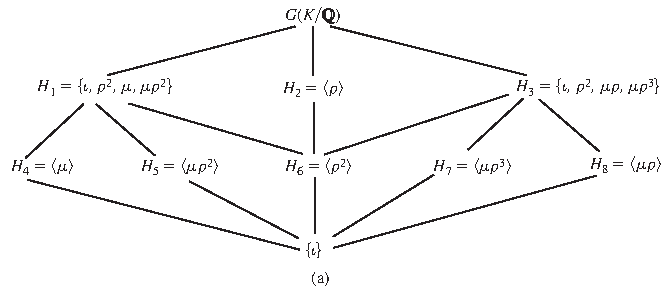
\includegraphics[width=0.917\linewidth,height=.8\textheight,keepaspectratio]{assets/p392_00.pdf}\end{center}
\end{BookFloat}

\begin{BookFloat}{47_illustrations_of_galois_theory-p392-1}
\begin{center}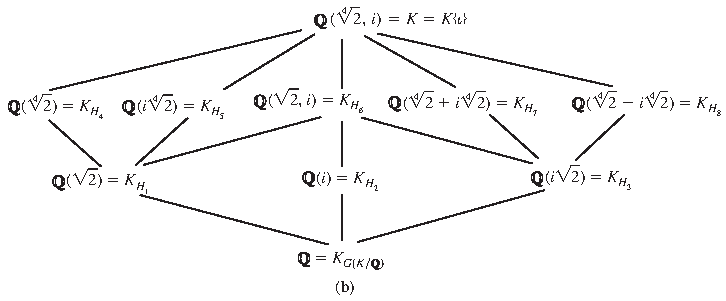
\includegraphics[width=0.995\linewidth,height=.8\textheight,keepaspectratio]{assets/p392_01.pdf}\end{center}
\begin{center}\small\textbf{47.6 Figure}\end{center}
\end{BookFloat}

(a) Group diagram. (b) Field diagram.

\noindent The conjugates of \BookInline{\gamma = \alpha + i\alpha } are thus \BookInline{\alpha + i\alpha,\allowbreak i\alpha - \alpha,\allowbreak - \alpha - i\alpha,\allowbreak } and \BookInline{- i\alpha + \alpha.} Hence

\begin{center}\begin{adjustbox}{max width=\linewidth}\BookInline{\displaystyle \begin{aligned}\;\text{irr}\;(\gamma ,\allowbreak \mathbb{Q})&= [(x- (\alpha + i\alpha ))(x- (i\alpha - \alpha ))] \\ &\cdot [(x- (- \alpha - i\alpha ))(x- (- i\alpha + \alpha ))] \\ &= (x^{2}- 2i\alpha x- 2\alpha ^{2})(x^{2}+ 2i\alpha x- 2\alpha ^{2}) \\ &= x^{4}+ 4\alpha ^{4}= x^{4}+ 8.\end{aligned}}\end{adjustbox}\end{center} \BookEnd{\blacktriangle}

We have seen examples in which the splitting field of a quartic (4th degree) polynomial over a field \BookInline{F} is an extension of \BookInline{F} of degree 8 (Example 47.3) and of degree 24 (Theorem 47.2, with \BookInline{n= 4).} The degree of an extension of a field \BookInline{F} that is a splitting field of a quartic over \BookInline{F} must always divide \BookInline{4!= 24.} The splitting field of \BookInline{(x- 2)^{4}} over \BookInline{\mathbb{Q}} is \BookInline{\mathbb{Q},\allowbreak } an extension of degree 1, and the splitting field of \BookInline{(x^{2}- 2)^{2}} over \BookInline{\mathbb{Q}} is \BookInline{\mathbb{Q}(\sqrt{2}),\allowbreak } an extension of degree 2. Our last example will give an extension of degree 4 for the splitting field of a quartic.

\BookLabel{47.7 Example} Consider the splitting field of \BookInline{x^{4}+ 1} over \BookInline{\mathbb{Q}.} By Theorem 28.12, we can show that \BookInline{x^{4}+ 1} is irreducible over \BookInline{\mathbb{Q},\allowbreak } by arguing that it does not factor in \BookInline{\mathbb{Z}[x].(}See Exercise 1.) The work on complex numbers in Section 3 shows that the zeros of \BookInline{x^{4}+ 1} are \BookInline{(1\pm } \BookInline{i)/\sqrt{2}} and \BookInline{(- 1\pm i)/\sqrt{2}.} A computation shows that if

\begin{center}\begin{adjustbox}{max width=\linewidth}\BookInline{\displaystyle \alpha = { \frac { 1 + i } { \sqrt { 2 } } } ,\allowbreak }\end{adjustbox}\end{center}

\end{BookBody}

% Source PDF page 393; original printed page 376
\BookSource{393}{376}
\BookNarrativetrue

\begin{BookBody}

\noindent then

\begin{center}\begin{adjustbox}{max width=\linewidth}\BookInline{\displaystyle \alpha ^ { 3 } = \frac { - 1 + i } { \sqrt { 2 } } ,\allowbreak  \qquad \alpha ^ { 5 } = \frac { - 1 - i } { \sqrt { 2 } } ,\allowbreak  \qquad \mathrm { a n d } \qquad \alpha ^ { 7 } = \frac { 1 - i } { \sqrt { 2 } } .}\end{adjustbox}\end{center}

\noindent Thus the splitting field \BookInline{K} of \BookInline{x^{4}+ 1} over \BookInline{\mathbb{Q}} is \BookInline{\mathbb{Q}(\alpha ),\allowbreak } and \BookInline{[K:\mathbb{Q}]= 4.} Let us compute \BookInline{G(K/\mathbb{Q})} and give the group and field diagrams. Since there exist automorphisms of \BookInline{K} mapping \BookInline{\alpha } onto each conjugate of \BookInline{\alpha,\allowbreak } and since an automorphism \BookInline{\sigma } of \BookInline{\mathbb{Q}(\alpha )} is completely determined by \BookInline{\sigma (\alpha ),\allowbreak } we see that the four elements of \BookInline{G(K/\mathbb{Q})} are defined by Table 47.8.

\begin{BookFloat}{47_illustrations_of_galois_theory-p393-3}
\begin{center}\small\textbf{47.8 Table}\end{center}
\begin{center}\begin{adjustbox}{max width=\linewidth}
\renewcommand{\arraystretch}{1.2}\setlength{\tabcolsep}{5pt}
\begin{tabular}{c|c|c|c|c}
 & \BookInline{\sigma _{1}} & \BookInline{\sigma _{3}} & \BookInline{\sigma _{5}} & \BookInline{\sigma _{7}}\\\hline
\BookInline{\alpha \to } & \BookInline{\alpha } & \BookInline{\alpha ^{3}} & \BookInline{\alpha ^{5}} & \BookInline{\alpha ^{7}}\\
\end{tabular}
\end{adjustbox}\end{center}
\end{BookFloat}

\noindent Since

\begin{center}\begin{adjustbox}{max width=\linewidth}\BookInline{\displaystyle (\sigma _{j}\sigma _{k})(\alpha )= \sigma _{j}(\alpha ^{k})= (\alpha ^{j})^{k}= \alpha ^{jk}}\end{adjustbox}\end{center}

\noindent and \BookInline{\alpha ^{8}= 1,\allowbreak } we see that \BookInline{G(K/\mathbb{Q})} is isomorphic to the group \BookInline{\{1,\allowbreak 3,\allowbreak 5,\allowbreak 7\}} under multiplication modulo 8. There are only two groups of order 4 up to isomorphism, the cyclic group and the Klein 4-group. Since each element of \BookInline{\{1,\allowbreak 3,\allowbreak 5,\allowbreak 7\}} has order 2 or \BookInline{1,\allowbreak G(K/\mathbb{Q})} is isomorphic with the Klein 4-group. The diagrams are given in Fig. 47.9.

\begin{BookFloat}{47_illustrations_of_galois_theory-p393-7}
\begin{center}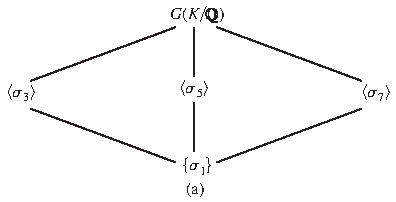
\includegraphics[width=0.543\linewidth,height=.8\textheight,keepaspectratio]{assets/p393_08.pdf}\end{center}
\end{BookFloat}

\begin{BookFloat}{47_illustrations_of_galois_theory-p393-8}
\begin{center}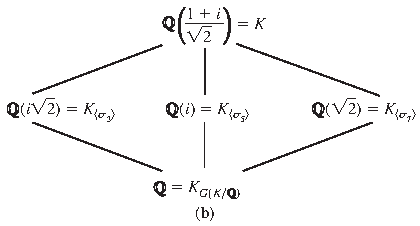
\includegraphics[width=0.576\linewidth,height=.8\textheight,keepaspectratio]{assets/p393_09.pdf}\end{center}
\begin{center}\small\textbf{47.9 Figure}\end{center}
\end{BookFloat}

(a) Group diagram. (b) Field diagram.

To find \BookInline{K_{\langle \sigma _{3}\rangle }}, it is only necessary to find an element of \BookInline{K} not in \BookInline{\mathbb{Q}} fixed by \BookInline{\{\sigma _{1},\allowbreak \sigma _{3}\},\allowbreak } since \BookInline{[K_{\langle \sigma _{3}\rangle }:\mathbb{Q}]= 2.} Clearly \BookInline{\sigma _{1}(\alpha )+ \sigma _{3}(\alpha )} is fixed by both \BookInline{\sigma _{1}} and \BookInline{\sigma _{3},\allowbreak } since \BookInline{\{\sigma _{1},\allowbreak \sigma _{3}\}} \BookInline{= \langle \sigma _{3}\rangle } is a group. We have

\begin{center}\begin{adjustbox}{max width=\linewidth}\BookInline{\displaystyle \sigma _{1}(\alpha )+ \sigma _{3}(\alpha )= \alpha + \alpha ^{3}= i\sqrt{2}.}\end{adjustbox}\end{center}

\noindent Similarly,

\begin{center}\begin{adjustbox}{max width=\linewidth}\BookInline{\displaystyle \sigma _{1}(\alpha )+ \sigma _{7}(\alpha )= \alpha + \alpha ^{7}= \sqrt{2}}\end{adjustbox}\end{center}

\end{BookBody}

% Source PDF page 394; original printed page 377
\BookSource{394}{377}
\BookNarrativetrue

\begin{BookBody}

\noindent is fixed by \BookInline{\langle \sigma _{7}\rangle = \{\sigma _{1},\allowbreak \sigma _{7}\}.} This technique is of no use in finding \BookInline{E_{\langle \sigma _{5}\rangle }}, for

\begin{center}\begin{adjustbox}{max width=\linewidth}\BookInline{\displaystyle \sigma _{1}(\alpha )+ \sigma _{5}(\alpha )= \alpha + \alpha ^{5}= 0,\allowbreak }\end{adjustbox}\end{center}

\noindent and \BookInline{0\in \mathbb{Q}.} But by a similar argument\BookInline{,\allowbreak \sigma _{1}(\alpha )\sigma _{5}(\alpha )} is fixed by both \BookInline{\sigma _{1}} and \BookInline{\sigma _{5},\allowbreak } and

\begin{center}\begin{adjustbox}{max width=\linewidth}\BookInline{\displaystyle \sigma _{1}(\alpha )\sigma _{5}(\alpha )= \alpha \alpha ^{5}= - i.}\end{adjustbox}\end{center}

\noindent Thus \BookInline{\mathbb{Q}(- i)= \mathbb{Q}(i)} is the field we are after. \BookEnd{\blacktriangle}

\end{BookBody}

\BookNarrativefalse

\begin{BookBody}

\BookExerciseTitle{47}

\BookTextHeading{\textbf{Computations (requiring more than the usual amount of theory)}  }

\BookExercise{1.}{Show that \BookInline{x^{4}+ 1} is irreducible in \BookInline{\mathbb{Q}[x],\allowbreak } as we asserted in Example 47.7.}

\BookExercise{2.}{Verify that the intermediate fields given in the field diagram in Fig. 47.6 are correct. (Some are verified in the text. Verify the rest.)}

\BookExercise{3.}{For each field in the field diagram in Fig. 47.6, find a primitive element generating the field over \BookInline{\mathbb{Q}(}see Theorem 45.13) and give its irreducible polynomial over \BookInline{\mathbb{Q}.}}

\BookExercise{4.}{Let \BookInline{\zeta } be a primitive 5th root of unity in \BookInline{\mathbb{C}.}}

\BookExercise{a.}{Show that \BookInline{\mathbb{Q}(\zeta )} is the splitting field of \BookInline{x^{5}- 1} over \BookInline{\mathbb{Q}.}}

\BookExercise{b.}{Show that every automorphism of \BookInline{K= \mathbb{Q}(\zeta )} maps \BookInline{\zeta } onto some power \BookInline{\zeta ^{r}} of \BookInline{\zeta.}}

\BookExercise{c.}{Using part (b), describe the elements of \BookInline{G(K/\mathbb{Q}).}}

\BookExercise{d.}{Give the group and field diagrams for \BookInline{\mathbb{Q}(\zeta )} over \BookInline{\mathbb{Q},\allowbreak } computing the intermediate fields as we did in Examples 47.3 and 47.7.}

\BookExercise{5.}{Describe the group of the polynomial \BookInline{(x^{5}- 2)\in (\mathbb{Q}(\zeta ))[x]} over \BookInline{\mathbb{Q}(\zeta ),\allowbreak } where \BookInline{\zeta } is a primitive 5th root of unity.}

\BookExercise{6.}{Repcat Exercise 4 for \BookInline{\zeta } a primitive 7th root of unity in \BookInline{\mathbb{C}.}}

\BookExercise{7.}{In the easiest way possible, describe the group of the polynomial}

\begin{center}\begin{adjustbox}{max width=\linewidth}\BookInline{\displaystyle (x^{8}- 1)\in \mathbb{Q}[x]}\end{adjustbox}\end{center}

\noindent over \BookInline{\mathbb{Q}.}

\BookExercise{8.}{Find the splitting field \BookInline{K} in \BookInline{\mathbb{C}} of the polynomial \BookInline{(x^{4}- 4x^{2}- 1)\in \mathbb{Q}[x].} Compute the group of the polynomial over \BookInline{\mathbb{Q}} and exhibit the correspondence between the subgroups of \BookInline{G(K/\mathbb{Q})} and the intermediate fields. In other words, do the complete job.}

\BookExercise{9.}{Express each of the following symmetric functions in \BookInline{y_{1},\allowbreak y_{2},\allowbreak y_{3}} over \BookInline{\mathbb{Q}} as a rational function of the elementary symmetric functions \BookInline{s_{1},\allowbreak s_{2},\allowbreak s_{3}.}}

\BookExercise{a.}{\textbf{a}\BookInline{.y_{1}^{2}+ y_{2}^{2}+ y_{3}^{2}}}

\noindent \textbf{b.} \BookInline{\frac{y_{1}}{y_{2}}+\frac{y_{2}}{y_{1}}+\frac{y_{1}}{y_{3}}+\frac{y_{3}}{y_{1}}+\frac{y_{2}}{y_{3}}+\frac{y_{3}}{y_{2}}}

\BookExercise{10.}{Let \BookInline{\alpha _{1},\allowbreak \alpha _{2},\allowbreak \alpha _{3}} be the zeros in \BookInline{\mathbb{C}} of the polynomial}

\begin{center}\begin{adjustbox}{max width=\linewidth}\BookInline{\displaystyle (x^{3}- 4x^{2}+ 6x- 2)\in \mathbb{Q}[x].}\end{adjustbox}\end{center}

\noindent Find the polynomial having as zeros precisely the following:

\BookExercise{a.}{\textbf{a}\BookInline{.\alpha _{1}+ \alpha _{2}+ \alpha _{3}}}

\BookExercise{b.}{\textbf{b}\BookInline{.\alpha _{1}^{2},\allowbreak \alpha _{2}^{2},\allowbreak \alpha _{3}^{2}}}

\BookTextHeading{\textbf{Theory}}

\BookExercise{11.}{Show that every finite group is isomorphic to some Galois group \BookInline{G(K/F)} for some finite normal extension \BookInline{K} of some field \BookInline{F.}}

\end{BookBody}

% Continuation on source PDF page 395, preceding Section 48
\BookNarrativefalse

\begin{BookBody}

\BookExercise{12.}{Let \BookInline{f(x)\in F[x]} be a monic polynomial of degree \BookInline{n} having all its irreducible factors separable over \BookInline{F.} Let \BookInline{K} be the splitting field of \BookInline{f(x)} over \BookInline{F,\allowbreak } and suppose that \BookInline{f(x)} factors in \BookInline{K[x]} into}

\begin{center}\begin{adjustbox}{max width=\linewidth}\BookInline{\displaystyle \prod _{i= 1}^{n}(x- \alpha _{i}).}\end{adjustbox}\end{center}

Let

\begin{center}\begin{adjustbox}{max width=\linewidth}\BookInline{\displaystyle \Delta (f)= \prod _{i<j}(\alpha _{i}- \alpha _{j});}\end{adjustbox}\end{center}

the product \BookInline{(\Delta (f))^{2}} is the\textbf{ discriminant of} \BookInline{f(x).}

\BookExercise{a.}{Show that \BookInline{\Delta (f)= 0} if and only if \BookInline{f(x)} has as a factor the square of some irreducible polynomial in \BookInline{F[x].}}

\BookExercise{b.}{Show that \BookInline{(\Delta (f))^{2}\in F.}}

\BookExercise{c.}{\textbf{c}\BookInline{.G(K/F)} may be viewed as a subgroup of \BookInline{\overline{S_{n}},\allowbreak } where \BookInline{\overline{S_{n}}} is the group of all permutations of \BookInline{\{\alpha _{i}\mid i= 1,\allowbreak \cdots,\allowbreak n\}.} Show that \BookInline{G(K/F),\allowbreak } when viewed in this fashion, is a subgroup of \BookInline{\overline{A_{n}},\allowbreak } the group formed by all even permutations of \BookInline{\{\alpha _{i}\mid i= 1,\allowbreak \cdots,\allowbreak n\},\allowbreak } if and only if \BookInline{\Delta (f)\in F.}}

\BookExercise{13.}{An element of \BookInline{\mathbb{C}} is an\textbf{ algebraic integer} if it is a zero of some\textit{ monic} polynomial in \BookInline{\mathbb{Z}[x].} Show that the set of all algebraic integers forms a subring of \BookInline{\mathbb{C}.}}

\end{BookBody}
\ifdefined\BookMaster\let\BookFinish\relax\else\def\BookFinish{\end{document}}\fi\BookFinish

\clearpage
% !TeX program = xelatex
\ifdefined\BookMaster\else
\documentclass[11pt,oneside]{article}
% !TeX program = xelatex
\usepackage[b5paper,left=22mm,right=22mm,top=20mm,bottom=22mm,footskip=11mm]{geometry}
\usepackage{fontspec}
\setmainfont{TeX Gyre Termes}
\setsansfont{TeX Gyre Heros}
\usepackage{amsmath,amssymb,mathtools,amsthm}
\renewcommand{\cdots}{\mathinner{\cdotp\cdotp\cdotp}}
\usepackage{graphicx,adjustbox,array,booktabs,longtable,multirow,enumitem,changepage,needspace}
\usepackage[table]{xcolor}
\usepackage{fancyhdr}
\raggedbottom
\interfootnotelinepenalty=10000
\newcommand{\BookFootnote}[2]{\begingroup\renewcommand{\thefootnote}{\fnsymbol{footnote}}\footnote[#1]{#2}\endgroup}
\newcommand{\BookFootnoteMark}[1]{\begingroup\renewcommand{\thefootnote}{\fnsymbol{footnote}}\footnotemark[#1]\endgroup}
\newcommand{\BookFootnoteText}[2]{\begingroup\renewcommand{\thefootnote}{\fnsymbol{footnote}}\footnotetext[#1]{#2}\endgroup}
\newenvironment{BookFloat}[1]{\par\addvspace{.6\baselineskip}\noindent\def\BookFloatID{#1}\begin{minipage}{\linewidth}\phantomsection\label{bookfloat:#1:start}}{\phantomsection\label{bookfloat:\BookFloatID:end}\end{minipage}\par\addvspace{.6\baselineskip}}

\usepackage[unicode,hidelinks]{hyperref}
\pagestyle{fancy}
\fancyhf{}
\newcommand{\BookFooter}{}
\fancyfoot[L]{\parbox[b]{\dimexpr\textwidth-15mm}{\footnotesize\BookFooter}}
\fancyfoot[R]{\footnotesize\thepage}
\renewcommand{\headrulewidth}{0pt}
\renewcommand{\footrulewidth}{0pt}
\setlength{\parindent}{0pt}
\setlength{\parskip}{0.2em}
\setlength{\emergencystretch}{3em}
\setlist{nosep,leftmargin=1.7em,labelsep=.65em}
\newif\ifBookNarrative
\BookNarrativetrue
\newenvironment{BookBody}{\setlength{\parindent}{0pt}}{}
\newcommand{\BookStatement}[1]{\par\addvspace{.6\baselineskip}\noindent #1\enspace\ignorespaces}
\newcommand{\BookLabel}[1]{\par\addvspace{.6\baselineskip}\needspace{3\baselineskip}\noindent\textbf{#1}\quad\ignorespaces}
\newcommand{\BookHeading}[1]{\par\addvspace{\baselineskip}\needspace{4\baselineskip}\noindent{\large\bfseries #1}\par\medskip}
\newcommand{\BookSubheading}[1]{\par\addvspace{.7\baselineskip}\needspace{3\baselineskip}\noindent{\bfseries #1}\par\smallskip}
\newcommand{\BookTextHeading}[1]{\par\addvspace{.7\baselineskip}\needspace{3\baselineskip}\noindent #1\par\smallskip}
\newcommand{\BookSectionTitle}[2]{\par\addvspace{1.2\baselineskip}\needspace{5\baselineskip}\noindent\colorbox{gray!25}{\sffamily\bfseries\small SECTION #1}\quad{\large\bfseries #2}\par\medskip}
\newcommand{\BookExerciseTitle}[1]{\par\addvspace{\baselineskip}\needspace{4\baselineskip}\noindent{\color{gray}\rule{1.5mm}{1.5mm}}\enspace{\large\bfseries Exercises #1}\par\medskip}
\newcommand{\BookBullet}[1]{\begin{list}{\textbullet}{\setlength{\leftmargin}{1.7em}\setlength{\labelwidth}{1em}\setlength{\labelsep}{.7em}\setlength{\topsep}{0pt}\setlength{\parsep}{0pt}\setlength{\itemsep}{0pt}}\item #1\end{list}}
\newcommand{\BookExercise}[2]{\begin{list}{\textbf{#1}}{\setlength{\leftmargin}{2.2em}\setlength{\labelwidth}{1.5em}\setlength{\labelsep}{.7em}\setlength{\topsep}{.15em}\setlength{\parsep}{0pt}\setlength{\itemsep}{0pt}}\item #2\end{list}}
\newcommand{\BookEnd}[1]{\unskip\nobreak\hfill\ensuremath{#1}}
\newcommand{\BookSource}[2]{\phantomsection\label{sourcepage:#1}} % Source-page anchors, retained through reflow.
\usepackage{multicol}
\usepackage{tikz}
\newcommand{\BookPartEntry}[2]{\par\noindent\makebox[17mm][l]{\bfseries Section #1}#2\par}
\newcommand{\BookPartTitle}[3]{\par\bigskip\noindent\begin{tikzpicture}\node[anchor=north west,inner sep=0pt,outer sep=0pt] (bookpart) at (0,0) {\begin{minipage}{\dimexpr\linewidth-.5pt}\hspace*{26mm}\begin{minipage}[t]{\dimexpr\linewidth-26mm}\begin{adjustbox}{max width=\linewidth}{\fontsize{20}{24}\selectfont\bfseries #2}\end{adjustbox}\par\vspace{6mm}\hrule\vspace{6mm}{\sffamily\footnotesize\setlength{\parskip}{.3em}#3}\vspace{3mm}\end{minipage}\end{minipage}};\path[shade,top color=gray!60,bottom color=white] (0,0) rectangle ([xshift=24mm]bookpart.south west);\node[anchor=north,font=\sffamily\bfseries\small] at (12mm,-2mm) {PART};\node[anchor=north,font=\sffamily\bfseries\Huge] at (12mm,-7mm) {#1};\end{tikzpicture}\par\bigskip}
\newsavebox{\BookMathBox}
\makeatletter
\newcommand{\BookInline}[1]{\leavevmode\hskip0pt\relax\begingroup\in@{\begin}{#1}\ifin@\sbox{\BookMathBox}{\(#1\)}\ifdim\wd\BookMathBox>\dimexpr\linewidth-1em\relax\resizebox{\dimexpr\linewidth-1em\relax}{!}{\usebox{\BookMathBox}}\else\(#1\)\fi\else\in@{\left}{#1}\ifin@\sbox{\BookMathBox}{\(#1\)}\ifdim\wd\BookMathBox>\dimexpr\linewidth-1em\relax\resizebox{\dimexpr\linewidth-1em\relax}{!}{\usebox{\BookMathBox}}\else\(#1\)\fi\else\(#1\)\fi\fi\endgroup\hskip0pt\relax}
\makeatother
\DeclareMathOperator{\Aut}{Aut}
\DeclareMathOperator{\End}{End}
\DeclareMathOperator{\Hom}{Hom}
\DeclareMathOperator{\GF}{GF}
\DeclareMathOperator{\irr}{irr}
\DeclareMathOperator{\lt}{lt}
\DeclareMathOperator{\lp}{lp}
\providecommand{\textcircled}[1]{\textnormal{(#1)}}

\begin{document}
\fi
\renewcommand{\BookFooter}{Section 48 Cyclotomic Extensions}
\pdfbookmark[0]{Section 48 Cyclotomic Extensions}{48_cyclotomic_extensions}
\ifdefined\BookMaster\else\setcounter{page}{378}\fi
% Source PDF page 395; original printed page 378
\BookSource{395}{378}
\BookNarrativetrue

\begin{BookBody}

\BookSectionTitle{48}{Cyclotomic Extensions}

\BookTextHeading{\textbf{The Galois Group of a Cyclotomic Extension}  }

\noindent In this section we consider subfields of the complex numbers obtained by adjoining roots of unity to the rational numbers\BookInline{,\allowbreak \mathbb{Q}.} We apply Galois theory to these extensions to determine which regular \BookInline{n-}gons are constructible.

\BookLabel{48.1 Definition} The splitting field of \BookInline{x^{n}- 1} over a field \BookInline{F} is the \BookInline{n}\textbf{th cyclotomic extension of} \BookInline{F.}\BookEnd{\blacksquare}

Since fields of characteristic zero are perfect, the splitting field\BookInline{,\allowbreak K,\allowbreak } of \BookInline{f(x)= x^{n}- 1} over \BookInline{\mathbb{Q}} is separable and thus a normal extension of \BookInline{\mathbb{Q}.} The distinct \BookInline{n} zeros of \BookInline{f(x)} form a cyclic group \BookInline{U_{n}.(}See Section 3.) We saw in Corollary 6.17 that the number of generators of a cyclic group of order \BookInline{n} is the number of positive integers less than \BookInline{n} that are relatively prime to \BookInline{n,\allowbreak } which we defined to be the Euler phi-function \BookInline{\varphi (n).} These \BookInline{\varphi (n)} generators are exactly the primitive \BookInline{n}th roots of unity.

\BookLabel{48.2 Definition} The polynomial

\begin{center}\begin{adjustbox}{max width=\linewidth}\BookInline{\displaystyle \Phi _{n}(x)= \prod _{i= 1}^{\varphi (n)}(x- \alpha _{i})}\end{adjustbox}\end{center}

\noindent where the \BookInline{\alpha _{i}} are the primitive \BookInline{n}th roots of unity in \BookInline{\mathbb{Q},\allowbreak } is the \BookInline{n}\textbf{th cyclotomic polynomial} \textbf{over} \BookInline{\mathbb{Q}.}\BookEnd{\blacksquare}

Let \BookInline{\sigma \in G(K/\mathbb{Q}).} Since an automorphism of the Galois group \BookInline{G(K/\mathbb{Q})} must permute the primitive \BookInline{n}th roots of unity, we see that \BookInline{\sigma _{x}(\Phi _{n}(x))= \Phi _{n}(x),\allowbreak } where \BookInline{\sigma _{x}:K[x]\to } \BookInline{K[x]} is the polynomial extension of \BookInline{\sigma.} Thus the coefficients of \BookInline{\Phi _{n}} are fixed by every \BookInline{\sigma \in G(K/\mathbb{Q}),\allowbreak } and therefore, all the coefficients of \BookInline{\Phi _{n}(x)} are rational numbers. That is, \BookInline{\Phi _{n}(x)\in \mathbb{Q}[x].} The \BookInline{n}th cyclotomic polynomial \BookInline{\Phi _{n}(x)} must divide \BookInline{x^{n}- 1,\allowbreak } so \BookInline{\Phi _{n}(x)\in } \BookInline{\mathbb{Z}[x]} by Theorem 28.12. For \BookInline{p} a prime number, Corollary 28.18 says that \BookInline{\Phi _{p}(x)} is irreducible over \BookInline{\mathbb{Q}.} Although we do not prove it here, it can be shown that \BookInline{\Phi _{n}(x)} is irreducible even when \BookInline{n\geq 2} is not a prime number.

\end{BookBody}

% Source PDF page 396; original printed page 379
\BookSource{396}{379}
\BookNarrativetrue

\begin{BookBody}

\BookTextHeading{\ensuremath{\blacksquare} \textbf{HISTORICAL NOTE}  }

\noindent Carl Gauss considered cyclotomic polynomials in the final chapter of his\textit{ Disquisitiones} \textit{Arithmeticae} of 1801. In that chapter, he gave a constructive procedure for actually determining the roots of \BookInline{\Phi _{p}(x)} in the case where \BookInline{p} is prime. Gauss’s method, which became an important example for Galois in the development of the general theory, was to solve a series of auxiliary equations, each of degree a prime factor of \BookInline{p- 1,\allowbreak } with the coefficients of each in turn being determined by the roots of the previous equation. Gauss, of course, knew that the roots of \BookInline{\Phi _{p}(x)} were all powers of one of them, say \BookInline{\zeta.} He determined the auxiliary equations by taking certain sets of sums of the roots \BookInline{\zeta ^{j},\allowbreak } which were the desired roots of these equations. For example, in the case where \BookInline{p= 19(}and \BookInline{p- 1= 18= } \BookInline{3\times 3\times 2),\allowbreak } Gauss needed to find two equations of degree 3 and one of degree 2 as his auxiliaries.

It turned out that the first one had the three roots\BookInline{,\allowbreak \alpha _{1}= \zeta + \zeta ^{8}+ \zeta ^{7}+ \zeta ^{18}+ \zeta ^{11}+ \zeta ^{12},\allowbreak \alpha _{2}= } \BookInline{\zeta ^{2}+ \zeta ^{16}+ \zeta ^{14}+ \zeta ^{17}+ \zeta ^{3}+ \zeta ^{5},\allowbreak } and \BookInline{\alpha _{3}= \zeta ^{4}+ } \BookInline{\zeta ^{13}+ \zeta ^{9}+ \zeta ^{15}+ \zeta ^{6}+ \zeta ^{10}.} In fact, these three values are the roots of the cubic equation \BookInline{x^{3}+ x^{2}- } \BookInline{6x- 7.} Gauss then found a second cubic equation, with coefficients involving the \BookInline{\alpha }’s, whose roots were sums of two of the powers of \BookInline{\zeta,\allowbreak } and finally a quadratic equation, whose coefficients involved the roots of the previous equation, which had \BookInline{\zeta } as one of its roots. Gauss then asserted (without a complete proof) that each auxiliary equation can in turn be reduced to an equation of the form \BookInline{x^{m}- A,\allowbreak } which clearly can be solved by radicals. That is, he showed that the solvability of the Galois group in this case, the cyclic group of order \BookInline{p- 1,\allowbreak } implied that the cyclotomic equation was solvable in terms of radicals. (See Section 49.)

Let \BookInline{i} be the usual complex zero of \BookInline{x^{2}+ 1.} Our work with complex numbers in Section 3 shows that

\begin{center}\begin{adjustbox}{max width=\linewidth}\BookInline{\displaystyle \left( \cos \frac{2\pi}{n} + i \sin \frac{2\pi}{n} \right)^n = \cos 2\pi + i \sin 2\pi = 1,\allowbreak }\end{adjustbox}\end{center}

\noindent so cos\BookInline{(2\pi /n)+ i} sin\BookInline{(2\pi /n)} is an \BookInline{n}th root of unity. The least integer \BookInline{m} such that (cos\BookInline{(2\pi /n)+ i} sin\BookInline{(2\pi /n))^{m}= 1} is \BookInline{n.} \textit{Thus} cos\BookInline{(2\pi /n)+ i} sin\BookInline{(2\pi /n)} \textit{is} \BookInline{a} \textit{primitive} n\textit{th} \textit{root of unity}\BookInline{,\allowbreak a} \textit{zero of}

\begin{center}\begin{adjustbox}{max width=\linewidth}\BookInline{\displaystyle \Phi _{n}(x)\in \mathbb{Q}[x].}\end{adjustbox}\end{center}

\BookLabel{48.3 Example} A primitive 8th root of unity in \BookInline{\mathbb{C}} is

\begin{center}\begin{adjustbox}{max width=\linewidth}\BookInline{\displaystyle \begin{aligned}\zeta &= \cos \frac{2\pi}{8} + i \sin \frac{2\pi}{8} \\&= \cos \frac{\pi}{4} + i \sin \frac{\pi}{4} \\&= \frac{1}{\sqrt{2}} + i \frac{1}{\sqrt{2}} = \frac{1 + i}{\sqrt{2}}.\end{aligned}}\end{adjustbox}\end{center}

\noindent By the theory of cyclic groups, in particular by Corollary 6.17, all the primitive 8th roots of unity in \BookInline{\mathbb{Q}} are \BookInline{\zeta,\allowbreak \zeta ^{3},\allowbreak \zeta ^{5},\allowbreak } and \BookInline{\zeta ^{7},\allowbreak } so

\begin{center}\begin{adjustbox}{max width=\linewidth}\BookInline{\displaystyle \Phi _{8}(x)= (x- \zeta )(x- \zeta ^{3})(x- \zeta ^{5})(x- \zeta ^{7}).}\end{adjustbox}\end{center}

\noindent We can compute, directly from this expression\BookInline{,\allowbreak \Phi _{8}(x)= x^{4}+ 1(}see Exercise 1). Compare this with Example \BookInline{47.7.}\BookEnd{\blacktriangle}

Let us assume, without proof, that \BookInline{\Phi _{n}(x)} is irreducible over \BookInline{\mathbb{Q}.} Let

\begin{center}\begin{adjustbox}{max width=\linewidth}\BookInline{\displaystyle \zeta = \cos \frac{2\pi}{n} + i \sin \frac{2\pi}{n},\allowbreak }\end{adjustbox}\end{center}

\end{BookBody}

% Source PDF page 397; original printed page 380
\BookSource{397}{380}
\BookNarrativetrue

\begin{BookBody}

\noindent so that \BookInline{\zeta } is a primitive \BookInline{n}th root of unity. Note that \BookInline{\zeta } is a generator of the cyclic multiplicative group of order \BookInline{n} consisting of\textit{ all} \BookInline{n}th roots of unity. All the primitive \BookInline{n}th roots of unity, that is, all the generators of this group, are of the form \BookInline{\zeta ^{m}} for \BookInline{1\leq m<n} and \BookInline{m} relatively prime to \BookInline{n.} The field \BookInline{\mathbb{Q}(\zeta )} is the whole splitting field of \BookInline{x^{n}- 1} over \BookInline{\mathbb{Q}.} Let \BookInline{K= \mathbb{Q}(\zeta ).} If \BookInline{\zeta ^{m}} is another primitive \BookInline{n}th root of unity, then since \BookInline{\zeta } and \BookInline{\zeta ^{m}} are conjugate over \BookInline{\mathbb{Q},\allowbreak } there is an automorphism \BookInline{\tau _{m}} in \BookInline{G(K/\mathbb{Q})} mapping \BookInline{\zeta } onto \BookInline{\zeta ^{m}.} Let \BookInline{\tau _{r}} be the similar automorphism in \BookInline{G(K/\mathbb{Q})} corresponding to a primitive \BookInline{n}th root of unity \BookInline{\zeta ^{r}.} Then

\begin{center}\begin{adjustbox}{max width=\linewidth}\BookInline{\displaystyle (\tau _{m}\tau _{r})(\zeta )= \tau _{m}(\zeta ^{r})= (\tau _{m}(\zeta ))^{r}= (\zeta ^{m})^{r}= \zeta ^{rm}.}\end{adjustbox}\end{center}

\noindent This shows that composing automorphisms \BookInline{\tau _{m}} and \BookInline{\tau _{r}} corresponds to multiplying \BookInline{m} and \BookInline{r} modulo \BookInline{n.} In other words, the Galois group \BookInline{G(K/\mathbb{Q})} is isomorphic with the group of units in \BookInline{\mathbb{Z}_{n}} under multiplication, with the isomorphism mapping \BookInline{\tau _{m}} to \BookInline{m.} The units in \BookInline{\mathbb{Z}_{n}} are the numbers less than \BookInline{n} that are relatively prime to \BookInline{n.} Thus \BookInline{G(K/\mathbb{Q})} is an abelian group with \BookInline{\varphi (n)} elements.

Special cases of this material have appeared several times in the text and exercises. For example\BookInline{,\allowbreak \alpha } of Example 47.7 is a primitive 8th root of unity, and we made arguments in that example identical to those given here. We summarize these results in a theorem.

\BookLabel{48.4 Theorem} The Galois group of the \BookInline{n}th cyclotomic extension of \BookInline{\mathbb{Q}} has \BookInline{\varphi (n)} elements and is isomorphic to the group consisting of the positive integers less than \BookInline{n} and relatively prime to \BookInline{n} under multiplication modulo \BookInline{n.}

\BookLabel{48.5 Example} Example 47.7 illustrates this theorem, for it is easy to see that the splitting field of \BookInline{x^{4}+ 1} is the same as the splitting field of \BookInline{x^{8}- 1} over \BookInline{\mathbb{Q}.} This follows from the fact that \BookInline{\Phi _{8}(x)= x^{4}+ 1(}see Example 48.3 and Exercise \BookInline{1).}\BookEnd{\blacktriangle}

\BookLabel{48.6 Corollary} The Galois group of the \BookInline{p}th cyclotomic extension of \BookInline{\mathbb{Q}} for a prime \BookInline{p} is cyclic of order \BookInline{p- 1.}

\BookLabel{\textit{Proof}} By Theorem 48.4, the Galois group of the \BookInline{p}th cyclotomic extension of \BookInline{\mathbb{Q}} has \BookInline{\varphi (p)= } \BookInline{p- 1} elements, and is isomorphic to the group of positive integers less than \BookInline{p} and relatively prime to \BookInline{p} under multiplication modulo \BookInline{p.} This is exactly the multiplicative group \BookInline{\langle \mathbb{Z}_{p}^{\ast },\allowbreak \cdot \rangle } of nonzero elements of the field \BookInline{\mathbb{Z}_{p}} under field multiplication. By Corollary 28.7, this group is cyclic\BookInline{.}\BookEnd{\blacklozenge}

\BookTextHeading{\textbf{Constructible Polygons}  }

\noindent We conclude with an application determining which regular \BookInline{n-}gons are constructible with a compass and a straightedge. We saw in Section 41 that the regular \BookInline{n-}gon is constructible if and only if cos\BookInline{(2\pi /n)} is a constructible real number. Now let

\begin{center}\begin{adjustbox}{max width=\linewidth}\BookInline{\displaystyle \zeta = \cos { \frac { 2 \pi } { n } } + i \sin { \frac { 2 \pi } { n } } .}\end{adjustbox}\end{center}

\noindent Then

\begin{center}\begin{adjustbox}{max width=\linewidth}\BookInline{\displaystyle \frac{1}{\zeta} = \cos \frac{2\pi}{n} - i \sin \frac{2\pi}{n},\allowbreak }\end{adjustbox}\end{center}

\noindent for

\begin{center}\begin{adjustbox}{max width=\linewidth}\BookInline{\displaystyle \left( \cos \frac{2\pi}{n} + i \sin \frac{2\pi}{n} \right) \left( \cos \frac{2\pi}{n} - i \sin \frac{2\pi}{n} \right) = \cos^2 \frac{2\pi}{n} + \sin^2 \frac{2\pi}{n} = 1.}\end{adjustbox}\end{center}

\end{BookBody}

% Source PDF page 398; original printed page 381
\BookSource{398}{381}
\BookNarrativetrue

\begin{BookBody}

\noindent But then

\begin{center}\begin{adjustbox}{max width=\linewidth}\BookInline{\displaystyle \zeta + \frac { 1 } { \zeta } = 2 \cos \frac { 2 \pi } { n } .}\end{adjustbox}\end{center}

\noindent Thus Corollary 41.8 shows that the regular \BookInline{n-}gon is constructible only if \BookInline{\zeta + 1/\zeta } generates an extension of \BookInline{\mathbb{Q}} of degree a power of 2.

If \BookInline{K} is the splitting field of \BookInline{x^{n}- 1} over \BookInline{\mathbb{Q},\allowbreak } then \BookInline{[K:\mathbb{Q}]= \varphi (n),\allowbreak } by Theorem 48.4. If \BookInline{\sigma \in G(K/\mathbb{Q})} and \BookInline{\sigma (\zeta )= \zeta ^{r},\allowbreak } then

\begin{center}\begin{adjustbox}{max width=\linewidth}\BookInline{\displaystyle \begin{aligned} \sigma \Bigg ( \zeta + \frac{1}{\zeta} \Bigg ) &= \zeta^{r} + \frac{1}{\zeta^{r}} \\&= \Bigg ( \cos \frac{2 \pi r}{n} + i \sin \frac{2 \pi r}{n} \Bigg ) + \Bigg ( \cos \frac{2 \pi r}{n} - i \sin \frac{2 \pi r}{n} \Bigg ) \\&= 2 \cos \frac{2 \pi r}{n}.\\ \end{aligned}}\end{adjustbox}\end{center}

\noindent But for \BookInline{1<r<n,\allowbreak } we have 2 cos\BookInline{(2\pi r/n)= 2} cos\BookInline{(2\pi /n)} only in the case that \BookInline{r= n- 1.} Thus the only elements of \BookInline{G(K/\mathbb{Q})} carrying \BookInline{\zeta + 1/\zeta } onto itself are the identity automorphism and the automorphism \BookInline{\tau,\allowbreak } with \BookInline{\tau (\zeta )= \zeta ^{n- 1}= 1/\zeta.} This shows that the subgroup of \BookInline{G(K/\mathbb{Q})} leaving \BookInline{\mathbb{Q}(\zeta + 1/\zeta )} fixed is of order 2, so by Galois theory,

\begin{center}\begin{adjustbox}{max width=\linewidth}\BookInline{\displaystyle \left[ \mathbb { Q } \bigg ( \zeta + \frac { 1 } { \zeta } \bigg ) : \mathbb { Q } \right] = \frac { \varphi ( n ) } { 2 } .}\end{adjustbox}\end{center}

\noindent \textit{Hence the regular} \BookInline{n-}\textit{gon is constructible only if} \BookInline{\varphi (n)/2,\allowbreak } \textit{and therefore also} \BookInline{\varphi (n),\allowbreak } \textit{is} \BookInline{a} \textit{power of 2}.

It can be shown by elementary arguments in number theory that if

\begin{center}\begin{adjustbox}{max width=\linewidth}\BookInline{\displaystyle n= 2^{\nu }p_{1}^{s_{1}}\cdots p_{t}^{s_{t}},\allowbreak }\end{adjustbox}\end{center}

\noindent where the \BookInline{p_{i}} are the distinct odd primes dividing \BookInline{n,\allowbreak } then

\begin{center}\begin{adjustbox}{max width=\linewidth}\BookInline{\displaystyle \varphi (n)= 2^{\nu - 1}p_{1}^{s_{1}- 1}\cdots p_{t}^{s_{t}- 1}(p_{1}- 1)\cdots (p_{t}- 1).(1)}\end{adjustbox}\end{center}

\noindent If \BookInline{\varphi (n)} is to be a power of 2, then every odd prime dividing \BookInline{n} must appear only to the first power and must be one more than a power of 2. Thus we must have each

\begin{center}\begin{adjustbox}{max width=\linewidth}\BookInline{\displaystyle p_{i}= 2^{m}+ 1}\end{adjustbox}\end{center}

\noindent for some \BookInline{m.} Since \BookInline{- 1} is a zero of \BookInline{x^{q}+ 1} for \BookInline{q} an odd prime\BookInline{,\allowbreak x+ 1} divides \BookInline{x^{q}+ 1} for \BookInline{q} an odd prime. Thus, if \BookInline{m= qu,\allowbreak } where \BookInline{q} is an odd prime, then \BookInline{2^{m}+ 1= (2^{u})^{q}+ 1} is divisible by \BookInline{2^{u}+ 1.} Therefore, for \BookInline{p_{i}= 2^{m}+ 1} to be prime, it must be that \BookInline{m} is divisible by 2 only, so \BookInline{p_{i}} has to have the form

\begin{center}\begin{adjustbox}{max width=\linewidth}\BookInline{\displaystyle p_{i}= 2^{(2^{k})}+ 1,\allowbreak }\end{adjustbox}\end{center}

\noindent a\textbf{ Fermat prime.} Fermat conjectured that these numbers \BookInline{2^{(2^{k})}+ 1} were prime for all nonnegative integers \BookInline{k.} Euler showed that while \BookInline{k= 0,\allowbreak 1,\allowbreak 2,\allowbreak 3,\allowbreak } and 4 give the primes 3, 5, 17, 257, and 65537, for \BookInline{k= 5,\allowbreak } the integer \BookInline{2^{(2^{s})}+ 1} is divisible by 641. It has been shown that for \BookInline{5\leq k\leq 19,\allowbreak } all the numbers \BookInline{2^{(2^{k})}+ 1} are composite. The case \BookInline{k= 20} is still unsolved as far as we know. For at least 60 values of \BookInline{k} greater than 20, including \BookInline{k= 9448,\allowbreak } it has been shown that \BookInline{2^{2^{k}}+ 1} is composite. It is unknown whether the number of Fermat primes is finite or infinite.

We have thus shown that the only regular \BookInline{n-}gons that might be constructible are those where the odd primes dividing \BookInline{n} are Fermat primes whose squares do not divide \BookInline{n.} In particular, the only regular \BookInline{p-}gons that might be constructible for \BookInline{p} a prime greater than 2 are those where \BookInline{p} is a Fermat prime.

\end{BookBody}

% Source PDF page 399; original printed page 382
\BookSource{399}{382}
\BookNarrativetrue

\begin{BookBody}

\BookLabel{48.7 Example} The regular 7-gon is not constructible, since 7 is not a Fermat prime. Similarly, the regular 18-gon is not constructible, for while 3 is a Fermat prime, its square divides \BookInline{18.}\BookEnd{\blacktriangle}

We now demonstrate that all these regular \BookInline{n-}gons that are candidates for being constructible are indeed actually constructible. Let \BookInline{\zeta } again be the primitive \BookInline{n}th root of unity cos\BookInline{(2\pi /n)+ i} sin\BookInline{(2\pi /n).} We saw above that

\begin{center}\begin{adjustbox}{max width=\linewidth}\BookInline{\displaystyle 2 \cos { \frac { 2 \pi } { n } } = \zeta + { \frac { 1 } { \zeta } } ,\allowbreak }\end{adjustbox}\end{center}

\noindent and that

\begin{center}\begin{adjustbox}{max width=\linewidth}\BookInline{\displaystyle \left[ \mathbb { Q } \bigg ( \zeta + \frac { 1 } { \zeta } \bigg ) : \mathbb { Q } \right] = \frac { \varphi ( n ) } { 2 } .}\end{adjustbox}\end{center}

\noindent Suppose now that \BookInline{\varphi (n)} is a power \BookInline{2^{s}} of 2. We saw above that \BookInline{\mathbb{Q}(\zeta + 1/\zeta )} is the subfield of \BookInline{K= \mathbb{Q}(\zeta )} fixed by \BookInline{H_{1}= \{\iota,\allowbreak \tau \},\allowbreak } where \BookInline{\iota } is the identity element of \BookInline{G(K/\mathbb{Q})} and \BookInline{\tau (\zeta )= } \BookInline{1/\zeta.} By Sylow theory, there exist additional subgroups \BookInline{H_{j}} of order \BookInline{2^{j}} of \BookInline{G(\mathbb{Q}(\zeta )/\mathbb{Q})} for \BookInline{j= 0,\allowbreak 2,\allowbreak 3,\allowbreak \cdots,\allowbreak s} such that

\begin{center}\begin{adjustbox}{max width=\linewidth}\BookInline{\displaystyle \{\iota \}= H_{0}<H_{1}<\cdots <H_{s}= G(\mathbb{Q}(\zeta )/\mathbb{Q}).}\end{adjustbox}\end{center}

\noindent By Galois theory,

\begin{center}\begin{adjustbox}{max width=\linewidth}\BookInline{\displaystyle \mathbb { Q } = K _ { H _ { s } } < K _ { H _ { s - 1 } } < \cdots < K _ { H _ { 1 } } = \mathbb { Q } \left( \zeta + \frac { 1 } { \zeta } \right) ,\allowbreak }\end{adjustbox}\end{center}

\noindent and \BookInline{[K_{H_{j- 1}}:K_{H}]= 2}. Note that \BookInline{(\zeta + 1/\zeta )\in \mathbb{R},\allowbreak } so \BookInline{\mathbb{Q}(\zeta + 1/\zeta )<\mathbb{R}.} If \BookInline{K_{H_{j- 1}}= K_{H_{j}}(\alpha _{j})}, then \BookInline{\alpha _{j}} is a zero of some \BookInline{(a_{j}x^{2}+ b_{j}x+ c_{j})\in K_{H_{j}}[x].} By the familiar “quadratic formula,” we have

\begin{center}\begin{adjustbox}{max width=\linewidth}\BookInline{\displaystyle K _ { H _ { j - 1 } } = K _ { H _ { j } } \big ( \sqrt { b _ { j } ^ { 2 } - 4 a _ { j } c _ { j } } \big ) .}\end{adjustbox}\end{center}

\noindent Since we saw in Section 41 that construction of square roots of positive constructible numbers can be achieved by a straightedge and a compass, we see that every element in \BookInline{\mathbb{Q}(\zeta + 1/\zeta ),\allowbreak } in particular cos\BookInline{(2\pi /n),\allowbreak } is constructible. Hence the regular \BookInline{n-}gons where \BookInline{\varphi (n)} is a power of 2 are constructible.

We summarize our work under this heading in a theorem.

\BookLabel{48.8 Theorem} The regular \BookInline{n-}gon is constructible with a compass and a straightedge if and only if all the odd primes dividing \BookInline{n} are Fermat primes whose squares do not divide \BookInline{n.}

\BookLabel{48.9 Example} The regular 60-gon is constructible, since \BookInline{60= (2^{2})(3)(5)} and 3 and 5 are both Fermat primes\BookInline{.}\BookEnd{\blacktriangle}

\end{BookBody}

\BookNarrativefalse

\begin{BookBody}

\BookExerciseTitle{48}

\BookTextHeading{\textbf{Computations}}

\BookExercise{1.}{Referring to Example 48.3, complete the indicated computation, showing that \BookInline{\Phi _{8}(x)= x^{4}+ 1.[}\textit{Suggestion:} Compute the product in terms of \BookInline{\zeta,\allowbreak } and then use the fact that \BookInline{\zeta ^{8}= 1} and \BookInline{\zeta ^{4}= - 1} to simplify the coefficients.]}

\BookExercise{2.}{Classify the group of the polynomial \BookInline{(x^{20}- 1)\in \mathbb{Q}[x]} over \BookInline{\mathbb{Q}} according to the Fundamental Theorem of Finitely Generated Abelian Groups. Theorem 9.12. [\textit{Hint:} Use Theorem 48.4.]}

\BookExercise{3.}{Using the formula for \BookInline{\varphi (n)} in terms of the factorization of \BookInline{n,\allowbreak } as given in Eq. (1), compute the indicated value: \textbf{a}\BookInline{.\varphi (60)} \textbf{b}\BookInline{.\varphi (1000)} \textbf{c}\BookInline{.\varphi (8100)}}

\BookExercise{4.}{Give the first 30 values of \BookInline{n\geq 3} for which the regular \BookInline{n-}gon is constructible with a straightedge and a compass.}

\end{BookBody}

% Source PDF page 400; original printed page 383
\BookSource{400}{383}
\BookNarrativefalse

\begin{BookBody}

\BookExercise{5.}{Find the smallest angle of integral degree, that is\BookInline{,\allowbreak 1^{\circ },\allowbreak 2^{\circ },\allowbreak 3^{\circ },\allowbreak } and so on, constructible with a straightedge and a compass. [\textit{Hint:} Constructing a \BookInline{1^{\circ }} angle amounts to constructing the regular 360-gon, and so on.]}

\BookExercise{6.}{Let \BookInline{K} be the splitting field of \BookInline{x^{12}- 1} over \BookInline{\mathbb{Q}.}}

\BookExercise{a.}{Find \BookInline{[K:\mathbb{Q}].}}

\BookExercise{b.}{Show that for \BookInline{\sigma \in G(K/\mathbb{Q}),\allowbreak \sigma ^{2}} is the identity automorphism. Classify \BookInline{G(K/\mathbb{Q})} according to the Fundamental Theorem 9.12 of finitely generated abelian groups.}

\BookTextHeading{\textbf{Concepts}}

\BookExercise{7.}{Determine whether each of the following is true or false.}

\BookExercise{a.}{\textbf{a}\BookInline{.\Phi _{n}(x)} is irreducible over every subfield of \BookInline{\mathbb{C}.}}

\BookExercise{b.}{Every zero in \BookInline{\mathbb{C}} of \BookInline{\Phi _{n}(x)} is a primitive \BookInline{n}th root of unity.}

\BookExercise{c.}{The group of \BookInline{\Phi _{n}(x)\in \mathbb{Q}[x]} over \BookInline{\mathbb{Q}} has order \BookInline{n.}}

\BookExercise{d.}{The group of \BookInline{\Phi _{n}(x)\in \mathbb{Q}[x]} over \BookInline{\mathbb{Q}} is abelian.}

\BookExercise{e.}{The Galois group of the splitting field of \BookInline{\Phi _{n}(x)} over \BookInline{\mathbb{Q}} has order \BookInline{\varphi (n).}}

\BookExercise{f.}{The regular 25-gon is constructible with a straightedge and a compass.}

\BookExercise{g.}{The regular 17-gon is constructible with a straightedge and a compass.}

\BookExercise{h.}{For a prime \BookInline{p,\allowbreak } the regular \BookInline{p-}gon is constructible if and only if \BookInline{p} is a Fermat prime.}

\BookExercise{i.}{All integers of the form \BookInline{2^{(2^{k})}+ 1} for nonnegative integers \BookInline{k} are Fermat primes.}

\BookExercise{j.}{All Fermat primes are numbers of the form \BookInline{2^{(2^{k})}+ 1} for nonnegative integers \BookInline{k.}}

\BookTextHeading{\textbf{Theory}}

\BookExercise{8.}{Show that}

\begin{center}\begin{adjustbox}{max width=\linewidth}\BookInline{\displaystyle x^{n}- 1= \prod _{d|n}\Phi _{d}(x)}\end{adjustbox}\end{center}

\noindent in \BookInline{\mathbb{Q}[x],\allowbreak } where the product is over all divisors \BookInline{d} of \BookInline{n.}

\BookExercise{9.}{Find the cyclotomic polynomial \BookInline{\Phi _{n}(x)} over \BookInline{\mathbb{Q}} for \BookInline{n= 1,\allowbreak 2,\allowbreak 3,\allowbreak 4,\allowbreak 5,\allowbreak } and 6. [\textit{Hint:} Use Exercise 8.]}

\BookExercise{10.}{Find \BookInline{\Phi _{12}(x)} in \BookInline{\mathbb{Q}[x].[}\textit{Hint:} Use Exercises 8 and 9.]}

\BookExercise{11.}{Show that in \BookInline{\mathbb{Q}[x],\allowbreak \Phi _{2n}(x)= \Phi _{n}(- x)} for odd integers \BookInline{n>1.[}\textit{Hint:} If \BookInline{\zeta } is a primitive \BookInline{n}th root of unity for \BookInline{n} odd, what is the order of \BookInline{- \zeta }?]}

\BookExercise{12.}{Let \BookInline{n,\allowbreak m\in \mathbb{Z}^{+ }} be relatively prime. Show that the splitting field in \BookInline{\mathbb{C}} of \BookInline{x^{nm}- 1} over \BookInline{\mathbb{Q}} is the same as the splitting field in \BookInline{\mathbb{C}} of \BookInline{(x^{n}- 1)(x^{m}- 1)} over \BookInline{\mathbb{Q}.}}

\BookExercise{13.}{Let \BookInline{n,\allowbreak m\in \mathbb{Z}^{+ }} be relatively prime. Show that the group of \BookInline{(x^{nm}- 1)\in \mathbb{Q}[x]} over \BookInline{\mathbb{Q}} is isomorphic to the direct product of the groups of \BookInline{(x^{n}- 1)\in \mathbb{Q}[x]} and of \BookInline{(x^{m}- 1)\in \mathbb{Q}[x]} over \BookInline{\mathbb{Q}.[}\textit{Hint:} Using Galois theory, show that the groups of \BookInline{x^{m}- 1} and \BookInline{x^{n}- 1} can both be regarded as subgroups of the group of \BookInline{x^{nm}- 1.} Then use Exercises 50 and 51 of Section 9.]}

\end{BookBody}
\ifdefined\BookMaster\let\BookFinish\relax\else\def\BookFinish{\end{document}}\fi\BookFinish

\clearpage
% !TeX program = xelatex
\ifdefined\BookMaster\else
\documentclass[11pt,oneside]{article}
% !TeX program = xelatex
\usepackage[b5paper,left=22mm,right=22mm,top=20mm,bottom=22mm,footskip=11mm]{geometry}
\usepackage{fontspec}
\setmainfont{TeX Gyre Termes}
\setsansfont{TeX Gyre Heros}
\usepackage{amsmath,amssymb,mathtools,amsthm}
\renewcommand{\cdots}{\mathinner{\cdotp\cdotp\cdotp}}
\usepackage{graphicx,adjustbox,array,booktabs,longtable,multirow,enumitem,changepage,needspace}
\usepackage[table]{xcolor}
\usepackage{fancyhdr}
\raggedbottom
\interfootnotelinepenalty=10000
\newcommand{\BookFootnote}[2]{\begingroup\renewcommand{\thefootnote}{\fnsymbol{footnote}}\footnote[#1]{#2}\endgroup}
\newcommand{\BookFootnoteMark}[1]{\begingroup\renewcommand{\thefootnote}{\fnsymbol{footnote}}\footnotemark[#1]\endgroup}
\newcommand{\BookFootnoteText}[2]{\begingroup\renewcommand{\thefootnote}{\fnsymbol{footnote}}\footnotetext[#1]{#2}\endgroup}
\newenvironment{BookFloat}[1]{\par\addvspace{.6\baselineskip}\noindent\def\BookFloatID{#1}\begin{minipage}{\linewidth}\phantomsection\label{bookfloat:#1:start}}{\phantomsection\label{bookfloat:\BookFloatID:end}\end{minipage}\par\addvspace{.6\baselineskip}}

\usepackage[unicode,hidelinks]{hyperref}
\pagestyle{fancy}
\fancyhf{}
\newcommand{\BookFooter}{}
\fancyfoot[L]{\parbox[b]{\dimexpr\textwidth-15mm}{\footnotesize\BookFooter}}
\fancyfoot[R]{\footnotesize\thepage}
\renewcommand{\headrulewidth}{0pt}
\renewcommand{\footrulewidth}{0pt}
\setlength{\parindent}{0pt}
\setlength{\parskip}{0.2em}
\setlength{\emergencystretch}{3em}
\setlist{nosep,leftmargin=1.7em,labelsep=.65em}
\newif\ifBookNarrative
\BookNarrativetrue
\newenvironment{BookBody}{\setlength{\parindent}{0pt}}{}
\newcommand{\BookStatement}[1]{\par\addvspace{.6\baselineskip}\noindent #1\enspace\ignorespaces}
\newcommand{\BookLabel}[1]{\par\addvspace{.6\baselineskip}\needspace{3\baselineskip}\noindent\textbf{#1}\quad\ignorespaces}
\newcommand{\BookHeading}[1]{\par\addvspace{\baselineskip}\needspace{4\baselineskip}\noindent{\large\bfseries #1}\par\medskip}
\newcommand{\BookSubheading}[1]{\par\addvspace{.7\baselineskip}\needspace{3\baselineskip}\noindent{\bfseries #1}\par\smallskip}
\newcommand{\BookTextHeading}[1]{\par\addvspace{.7\baselineskip}\needspace{3\baselineskip}\noindent #1\par\smallskip}
\newcommand{\BookSectionTitle}[2]{\par\addvspace{1.2\baselineskip}\needspace{5\baselineskip}\noindent\colorbox{gray!25}{\sffamily\bfseries\small SECTION #1}\quad{\large\bfseries #2}\par\medskip}
\newcommand{\BookExerciseTitle}[1]{\par\addvspace{\baselineskip}\needspace{4\baselineskip}\noindent{\color{gray}\rule{1.5mm}{1.5mm}}\enspace{\large\bfseries Exercises #1}\par\medskip}
\newcommand{\BookBullet}[1]{\begin{list}{\textbullet}{\setlength{\leftmargin}{1.7em}\setlength{\labelwidth}{1em}\setlength{\labelsep}{.7em}\setlength{\topsep}{0pt}\setlength{\parsep}{0pt}\setlength{\itemsep}{0pt}}\item #1\end{list}}
\newcommand{\BookExercise}[2]{\begin{list}{\textbf{#1}}{\setlength{\leftmargin}{2.2em}\setlength{\labelwidth}{1.5em}\setlength{\labelsep}{.7em}\setlength{\topsep}{.15em}\setlength{\parsep}{0pt}\setlength{\itemsep}{0pt}}\item #2\end{list}}
\newcommand{\BookEnd}[1]{\unskip\nobreak\hfill\ensuremath{#1}}
\newcommand{\BookSource}[2]{\phantomsection\label{sourcepage:#1}} % Source-page anchors, retained through reflow.
\usepackage{multicol}
\usepackage{tikz}
\newcommand{\BookPartEntry}[2]{\par\noindent\makebox[17mm][l]{\bfseries Section #1}#2\par}
\newcommand{\BookPartTitle}[3]{\par\bigskip\noindent\begin{tikzpicture}\node[anchor=north west,inner sep=0pt,outer sep=0pt] (bookpart) at (0,0) {\begin{minipage}{\dimexpr\linewidth-.5pt}\hspace*{26mm}\begin{minipage}[t]{\dimexpr\linewidth-26mm}\begin{adjustbox}{max width=\linewidth}{\fontsize{20}{24}\selectfont\bfseries #2}\end{adjustbox}\par\vspace{6mm}\hrule\vspace{6mm}{\sffamily\footnotesize\setlength{\parskip}{.3em}#3}\vspace{3mm}\end{minipage}\end{minipage}};\path[shade,top color=gray!60,bottom color=white] (0,0) rectangle ([xshift=24mm]bookpart.south west);\node[anchor=north,font=\sffamily\bfseries\small] at (12mm,-2mm) {PART};\node[anchor=north,font=\sffamily\bfseries\Huge] at (12mm,-7mm) {#1};\end{tikzpicture}\par\bigskip}
\newsavebox{\BookMathBox}
\makeatletter
\newcommand{\BookInline}[1]{\leavevmode\hskip0pt\relax\begingroup\in@{\begin}{#1}\ifin@\sbox{\BookMathBox}{\(#1\)}\ifdim\wd\BookMathBox>\dimexpr\linewidth-1em\relax\resizebox{\dimexpr\linewidth-1em\relax}{!}{\usebox{\BookMathBox}}\else\(#1\)\fi\else\in@{\left}{#1}\ifin@\sbox{\BookMathBox}{\(#1\)}\ifdim\wd\BookMathBox>\dimexpr\linewidth-1em\relax\resizebox{\dimexpr\linewidth-1em\relax}{!}{\usebox{\BookMathBox}}\else\(#1\)\fi\else\(#1\)\fi\fi\endgroup\hskip0pt\relax}
\makeatother
\DeclareMathOperator{\Aut}{Aut}
\DeclareMathOperator{\End}{End}
\DeclareMathOperator{\Hom}{Hom}
\DeclareMathOperator{\GF}{GF}
\DeclareMathOperator{\irr}{irr}
\DeclareMathOperator{\lt}{lt}
\DeclareMathOperator{\lp}{lp}
\providecommand{\textcircled}[1]{\textnormal{(#1)}}

\begin{document}
\fi
\renewcommand{\BookFooter}{Section 49 Insolvability of the Quintic}
\pdfbookmark[0]{Section 49 Insolvability of the Quintic}{49_insolvability_of_the_quintic}
\ifdefined\BookMaster\else\setcounter{page}{384}\fi
% Source PDF page 401; original printed page 384
\BookSource{401}{384}
\BookNarrativetrue

\begin{BookBody}

\BookSectionTitle{49}{Insolvability of the Quintic}

\BookTextHeading{\textbf{The Problem}  }

\noindent We are familiar with the fact that a quadratic polynomial \BookInline{f(x)= ax^{2}+ bx+ c,\allowbreak a\neq 0,\allowbreak } with real coefficients has \BookInline{(- b\pm \sqrt{b^{2}}- 4}\textit{ac}\BookInline{)/2a} as zeros in \BookInline{\mathbb{C}.} Actually, this is true for \BookInline{f(x)\in F[x],\allowbreak } where \BookInline{F} is any field of characteristic\BookInline{\neq 2} and the zeros are in \BookInline{F.} Exercise 4 asks us to show this. Thus, for example\BookInline{,\allowbreak (x^{2}+ 2x+ 3)\in \mathbb{Q}[x]} has its zeros in \BookInline{\mathbb{Q}(\sqrt{- }2).} You may wonder whether the zeros of a cubic polynomial over \BookInline{\mathbb{Q}} can also always be expressed in terms of radicals. The answer is yes, and indeed, even the zeros of a polynomial of degree 4 over \BookInline{\mathbb{Q}} can be expressed in terms of radicals. After mathematicians had tried for years to find the “radical formula” for zeros of a 5th degree polynomial, it was a triumph when Abel proved that a quintic need not be solvable by radicals. Our first job will be to describe precisely what this means. A large amount of the algebra we have developed is used in the forthcoming discussion.

\BookTextHeading{\textbf{Extensions by Radicals}  }

\BookLabel{49.1 Definition} An extension \BookInline{K} of a field \BookInline{F} is an\textbf{ extension of} \BookInline{F} \textbf{by radicals} if there are elements \BookInline{\alpha _{1},\allowbreak \cdots,\allowbreak \alpha _{r}\in K} and positive integers \BookInline{n_{1},\allowbreak \cdots,\allowbreak n_{r}} such that \BookInline{K= F(\alpha _{1},\allowbreak \cdots,\allowbreak \alpha _{r}),\allowbreak \alpha _{1}^{n_{1}}\in F} and \BookInline{\alpha _{i}^{n_{i}}\in F(\alpha _{1},\allowbreak \cdots,\allowbreak \alpha _{i- 1})} for \BookInline{1<i\leq r.} A polynomial \BookInline{f(x)\in F[x]} is\textbf{ solvable by rad}\textbf{icals over} \BookInline{F} if the splitting field \BookInline{E} of \BookInline{f(x)} over \BookInline{F} is contained in an extension of \BookInline{F} by radicals\BookInline{.}\BookEnd{\blacksquare}

A polynomial \BookInline{f(x)\in F(x)} is thus solvable by radicals over \BookInline{F} if we can obtain every zero of \BookInline{f(x)} by using a finite sequence of the operations of addition, subtraction, multiplication, division, and taking \BookInline{n_{i}}th roots, starting with elements of \BookInline{F.} Now to say that the quintic is not solvable in the classic case, that is, characteristic 0, is not to say that no quintic is solvable, as the following example shows.

\BookLabel{49.2 Example} The polynomial \BookInline{x^{5}- 1} is solvable by radicals over \BookInline{\mathbb{Q}.} The splitting field \BookInline{K} of \BookInline{x^{5}- 1} is generated over \BookInline{\mathbb{Q}} by a primitive 5th root \BookInline{\zeta } of unity. Then \BookInline{\zeta ^{5}= 1,\allowbreak } and \BookInline{K= \mathbb{Q}(\zeta ).} Similarly\BookInline{,\allowbreak x^{5}- 2} is solvable by radicals over \BookInline{\mathbb{Q},\allowbreak } for its splitting field over \BookInline{\mathbb{Q}} is generated by \BookInline{\sqrt { 2 }} and \BookInline{\zeta,\allowbreak } where \BookInline{\sqrt { 2 }} is the real zero of \BookInline{x^{5}- 2.}\BookEnd{\blacktriangle}

To say that the quintic is insolvable in the classic case means that there exists\textit{ some} polynomial of degree 5 with real coefficients that is not solvable by radicals. We shall show this.\textit{ We assume throughout this section that all fields mentioned have character}\textit{istic 0}.

The outline of the argument is as follows, and it is worthwhile to try to remember it.

\BookExercise{1.}{\textit{We shall show that} \BookInline{a} \textit{polynomial} \BookInline{f(x)\in F[x]} \textit{is solvable by radicals over} \BookInline{F(}\textit{if} \textit{and})\textit{ only if its splitting} \BookInline{\text{fi}eldE} \textit{over} \BookInline{F} \textit{has} \BookInline{a} \textit{solvable Galois group}. Recall that a solvable group is one having a composition series with\textit{ abelian} quotients. While this theorem goes both ways, we shall not prove the “if” part.}

\BookExercise{2.}{\textit{We shall show that there is} \BookInline{a} \textit{polynomial} \BookInline{f(x)\in \Phi [x]} \textit{of degree} 5\textit{ with} \BookInline{a} \textit{splitting} \BookInline{\text{fi}eldE} \textit{over} \BookInline{\mathbb{Q}} \textit{such that} \BookInline{G(E/\mathbb{Q})\simeq S_{5},\allowbreak } \textit{the symmetric group on} 5 \textit{letters}. Recall that a composition series for \BookInline{S_{5}} is \BookInline{\{\iota \}<A_{5}<S_{5}.} Since \BookInline{A_{5}} is not abelian, we will be done.}

\noindent The following lemma does most of our work for Step 1.

\BookLabel{49.3 Lemma} Let \BookInline{F} be a field of characteristic 0, and let \BookInline{a\in F.} If \BookInline{K} is the splitting field of \BookInline{x^{n}- a} over \BookInline{F,\allowbreak } then \BookInline{G(K/F)} is a solvable group.

\end{BookBody}

% Source PDF page 402; original printed page 385
\BookSource{402}{385}
\BookNarrativetrue

\begin{BookBody}

\BookTextHeading{\ensuremath{\blacksquare} \textbf{HISTORICAL NOTE}  }

\noindent The first publication of a formula for solving cubic equations in terms of radicals was in 1545 in the \BookInline{Ars} \textit{Magna} of Girolamo Cardano, although the initial discovery of the method is in part also due to Scipione del Ferro and Niccolo Tartaglia. Cardano’s student, Lodovico Ferrari, discovered a method for solving quartic equations by radicals, which also appeared in Cardano’s work.

\noindent After many mathematicians had attempted to solve quintics by similar methods, it was Joseph- Louis Lagrange who in 1770 first attempted a detailed analysis of the general principles underlying the solutions for polynomials of degree 3 and 4, and showed why these methods fail for those of higher degree. His basic insight was that in the former cases there were rational functions of the roots that took on two and three values, respectively, under all possible permutations of the roots, hence these rational functions could be written as roots of equations of degree less than that of the original. No such functions were evident in equations of higher degree.

The first mathematician to claim to have a proof of the insolvability of the quintic equation was Paolo Ruffini (1765–1822) in his algebra text of 1799. His proof was along the lines suggested by Lagrange, in that he in effect determined all of the subgroups of \BookInline{S_{5}} and showed how these subgroups acted on rational functions of the roots of the equation. Unfortunately, there were several gaps in his various published versions of the proof. It was Niels Henrik Abel who, in 1824 and 1826, published a complete proof, closing all of Ruffini’s gaps and finally settling this centuries-old question.

\BookLabel{\textit{Proof}} Suppose first that \BookInline{F} contains all the \BookInline{n}th roots of unity. By Corollary 28.7 the \BookInline{n}th roots of unity form a cyclic subgroup of \BookInline{\langle F^{\ast },\allowbreak \cdot \rangle.} Let \BookInline{\zeta } be a generator of the subgroup. (Actually, the generators are exactly the\textit{ primitive} \BookInline{n}th roots of unity.) Then the \BookInline{n}th roots of unity are

\begin{center}\begin{adjustbox}{max width=\linewidth}\BookInline{\displaystyle 1,\allowbreak \zeta ,\allowbreak \zeta ^{2},\allowbreak \cdots ,\allowbreak \zeta ^{n- 1}.}\end{adjustbox}\end{center}

\noindent If \BookInline{\beta \in F} is a zero of \BookInline{(x^{n}- a)\in F[x],\allowbreak } then all zeros of \BookInline{x^{n}- a} are

\begin{center}\begin{adjustbox}{max width=\linewidth}\BookInline{\displaystyle \beta ,\allowbreak \zeta \beta ,\allowbreak \zeta ^{2}\beta ,\allowbreak \cdots ,\allowbreak \zeta ^{n- 1}\beta .}\end{adjustbox}\end{center}

\noindent Since \BookInline{K= F(\beta ),\allowbreak } an automorphism \BookInline{\sigma } in \BookInline{G(K/F)} is determined by the value \BookInline{\sigma (\beta )} of the automorphism \BookInline{\sigma } on \BookInline{\beta.} Now if \BookInline{\sigma (\beta )= \zeta ^{i}\beta } and \BookInline{\tau (\beta )= \zeta ^{j}\beta,\allowbreak } where \BookInline{\tau \in G(K/F),\allowbreak } then

\begin{center}\begin{adjustbox}{max width=\linewidth}\BookInline{\displaystyle (\tau \sigma )(\beta )= \tau (\sigma (\beta ))= \tau (\zeta ^{i}\beta )= \zeta ^{i}\tau (\beta )= \zeta ^{i}\zeta ^{j}\beta ,\allowbreak }\end{adjustbox}\end{center}

\noindent since \BookInline{\zeta ^{i}\in F.} Similarly,

\begin{center}\begin{adjustbox}{max width=\linewidth}\BookInline{\displaystyle (\sigma \tau )(\beta )= \zeta ^{j}\zeta ^{i}\beta .}\end{adjustbox}\end{center}

\noindent Thus \BookInline{\sigma \tau = \tau \sigma,\allowbreak } and \BookInline{G(K/F)} is abelian and therefore solvable.

Now suppose that \BookInline{F} does not contain a primitive \BookInline{n}th root of unity. Let \BookInline{\zeta } be a generator of the cyclic group of \BookInline{n}th roots of unity under multiplication in \BookInline{F.} Let \BookInline{\beta } again be a zero of \BookInline{x^{n}- a.} Since \BookInline{\beta } and \BookInline{\zeta \beta } are both in the splitting field \BookInline{K} of \BookInline{x^{n}- a,\allowbreak \zeta = } \BookInline{(\zeta \beta )/\beta } is in \BookInline{K.} Let \BookInline{F^{\prime }= F(\zeta ),\allowbreak } so we have \BookInline{F<F^{\prime }\leq K.} Now \BookInline{F^{\prime }} is a normal extension of \BookInline{F,\allowbreak } since \BookInline{F^{\prime }} is the splitting field of \BookInline{x^{n}- 1.} Since \BookInline{F^{\prime }= F(\zeta ),\allowbreak } an automorphism \BookInline{\eta } in \BookInline{G(F^{\prime }/F)} is determined by \BookInline{\eta (\zeta ),\allowbreak } and we must have \BookInline{\eta (\zeta )= \zeta ^{i}} for some \BookInline{i,\allowbreak } since all zeros of \BookInline{x^{n}- 1} are powers of \BookInline{\zeta.} If \BookInline{\mu (\zeta )= \zeta ^{j}} for \BookInline{\mu \in G(F^{\prime }/F),\allowbreak } then

\begin{center}\begin{adjustbox}{max width=\linewidth}\BookInline{\displaystyle (\mu \eta )(\zeta )= \mu (\eta (\zeta ))= \mu (\zeta ^{i})= \mu (\zeta )^{i}= (\zeta ^{j})^{i}= \zeta ^{ij},\allowbreak }\end{adjustbox}\end{center}

\noindent and, similarly,

\begin{center}\begin{adjustbox}{max width=\linewidth}\BookInline{\displaystyle (\eta \mu )(\zeta )= \zeta ^{ij}.}\end{adjustbox}\end{center}

\end{BookBody}

% Source PDF page 403; original printed page 386
\BookSource{403}{386}
\BookNarrativetrue

\begin{BookBody}

\noindent Thus \BookInline{G(F^{\prime }/F)} is abelian. By Theorem 46.10,

\begin{center}\begin{adjustbox}{max width=\linewidth}\BookInline{\displaystyle \{\iota \}\leq G(K/F^{\prime })\leq G(K/F)}\end{adjustbox}\end{center}

\noindent is a normal series and hence a subnormal series of groups. The first part of the proof shows that \BookInline{G(K/F^{\prime })} is abelian, and Galois theory tells us that \BookInline{G(K/F)/G(K/F^{\prime })} is isomorphic to \BookInline{G(F^{\prime }/F),\allowbreak } which is abelian. Exercise 6 shows that if a group has a subnormal series of subgroups with abelian quotient groups, then any refinement of this series also has abelian quotient groups. Thus a composition series of \BookInline{G(K/F)} must have abelian quotient groups, so \BookInline{G(K/F)} is solvable\BookInline{.}\BookEnd{\blacklozenge}

\noindent The following theorem will complete Step 1 of our program.

\BookLabel{49.4 Theorem} Let \BookInline{F} be a field of characteristic zero, and let \BookInline{F\leq E\leq K\leq F,\allowbreak } where \BookInline{E} is a normal extension of \BookInline{F} and \BookInline{K} is an extension of \BookInline{F} by radicals. Then \BookInline{G(E/F)} is a solvable group.

\BookLabel{\textit{Proof}} We first show that \BookInline{K} is contained in a finite normal extension \BookInline{L} of \BookInline{F} by radicals and that the group \BookInline{G(L/F)} is solvable. Since \BookInline{K} is an extension of \BookInline{F} by radicals\BookInline{,\allowbreak K= } \BookInline{F(\alpha _{1},\allowbreak \cdots,\allowbreak \alpha _{r})} where \BookInline{\alpha _{i}^{n_{i}}\in F(\alpha _{1},\allowbreak \cdots,\allowbreak \alpha _{i- 1})} for \BookInline{1<i\leq r} and \BookInline{\alpha _{1}^{n_{1}}\in F.} To form \BookInline{L,\allowbreak } we first form the splitting field \BookInline{L_{1}} of \BookInline{f_{1}(x)= x^{n_{1}}- \alpha _{1}^{n_{1}}} over \BookInline{F.} Then \BookInline{L_{1}} is a normal extension of \BookInline{F,\allowbreak } and Lemma 49.3 shows that \BookInline{G(L_{1}/F)} is a solvable group. Now \BookInline{\alpha _{2}^{n_{2}}\in L_{1}} and we form the polynomial

\begin{center}\begin{adjustbox}{max width=\linewidth}\BookInline{\displaystyle f_{2}(x)= _{\sigma \in G}\prod _{(L_{1}/F)}[(x^{n_{2}}- \sigma (\alpha _{2})^{n_{2}}].}\end{adjustbox}\end{center}

\noindent Since this polynomial is invariant under action by any \BookInline{\sigma } in \BookInline{G(L_{1}/F),\allowbreak } we see that \BookInline{f_{2}(x)\in } \BookInline{F[x].} We let \BookInline{L_{2}} be the splitting field of \BookInline{f_{2}(x)} over \BookInline{L_{1}.} Then \BookInline{L_{2}} is a splitting field over \BookInline{F} also and is a normal extension of \BookInline{F} by radicals. We can form \BookInline{L_{2}} from \BookInline{L_{1}} via repeated steps as in Lemma 49.3, passing to a splitting field of \BookInline{x^{n_{2}}- \sigma (\alpha _{2})^{n_{2}}} at each step. By Lemma 49.3 and Exercise 7, we see that the Galois group over \BookInline{F} of each new extension thus formed continues to be solvable. We continue this process of forming splitting fields over \BookInline{F} in this manner: At stage \BookInline{i,\allowbreak } we form the splitting field of the polynomial

\begin{center}\begin{adjustbox}{max width=\linewidth}\BookInline{\displaystyle f_{i}(x)= _{\sigma \in G}\prod _{(L_{i- 1}/F)}[(x^{n_{i}}- \sigma (\alpha _{i})^{n_{i}}]}\end{adjustbox}\end{center}

\noindent over \BookInline{L_{i- 1}.} We finally obtain a field \BookInline{L= L_{r}} that is a normal extension of \BookInline{F} by radicals, and we see that \BookInline{G(L/F)} is a solvable group. We see from construction that \BookInline{K\leq L.}

To conclude, we need only note that by Theorem 46.8, we have \BookInline{G(E/F)\simeq G(L/F)/} \BookInline{G(L/E).} Thus \BookInline{G(E/F)} is a factor group, and hence a homomorphic image, of \BookInline{G(L/F).} Since \BookInline{G(L/F)} is solvable, Exercise 31 of Section 18 shows that \BookInline{G(E/F)} is solvable. \BookEnd{\blacklozenge}

\BookTextHeading{\textbf{The Insolvability of the Quintic}  }

\noindent It remains to find a polynomial \BookInline{f(x)\in \mathbb{Q}[x],\allowbreak } whose splitting field has Galois group \BookInline{S_{5}.} The polynomial \BookInline{f(x)= 2x^{5}- 5x^{4}+ 5} does the trick as we now show. To begin, we prove the following theorem that gives a simple condition for a subgroup of \BookInline{S_{5}} to actually be all of \BookInline{S_{5}.} We will use this theorem to show that the Galois group of the splitting field of \BookInline{f(x)} over \BookInline{\mathbb{Q}} is isomorphic with \BookInline{S_{5}.}

\BookLabel{49.5 Theorem} Let \BookInline{H} be a subgroup of \BookInline{S_{5}.} If \BookInline{H} has a transposition and a 5-cycle, then \BookInline{H= S_{5}.}

\BookLabel{\textit{Proof}} We can assume, by relabeling the points being permuted, that the 5-cycle (0, 1, 2, 3, 4) is in \BookInline{H} and the transposition \BookInline{(0,\allowbreak j),\allowbreak j\neq 0,\allowbreak } is also in \BookInline{H.} We think of \BookInline{S_{5}} as permuting the 
% Source PDF page 404; original printed page 387
\BookSource{404}{387}
elements in \BookInline{\mathbb{Z}_{5}.} By conjugating with the 5-cycle \BookInline{(0,\allowbreak 1,\allowbreak 2,\allowbreak 3,\allowbreak 4)^{r},\allowbreak } we have that for each \BookInline{0\leq r\leq 4,\allowbreak }

\end{BookBody}

\BookNarrativetrue

\begin{BookBody}

\begin{center}\begin{adjustbox}{max width=\linewidth}\BookInline{\displaystyle (0,\allowbreak 1,\allowbreak 2,\allowbreak 3,\allowbreak 4)^{r}(0,\allowbreak j)(0,\allowbreak 1,\allowbreak 2,\allowbreak 3,\allowbreak 4)^{- r}= (r,\allowbreak r+ j),\allowbreak }\end{adjustbox}\end{center}

\noindent where addition is in \BookInline{\mathbb{Z}_{5}.} Thus \BookInline{(0,\allowbreak j)} and \BookInline{(j,\allowbreak 2j)} are both in \BookInline{H;} and therefore

\begin{center}\begin{adjustbox}{max width=\linewidth}\BookInline{\displaystyle (0,\allowbreak j)(j,\allowbreak 2j)(0,\allowbreak j)= (0,\allowbreak 2j)\in H.}\end{adjustbox}\end{center}

\noindent As before, by conjugating \BookInline{(0,\allowbreak 2j)} with \BookInline{(0,\allowbreak 1,\allowbreak 2,\allowbreak 3,\allowbreak 4)^{r}} we have \BookInline{(r,\allowbreak r+ 2j)\in H} for \BookInline{0\leq r\leq 4.} Now,

\begin{center}\begin{adjustbox}{max width=\linewidth}\BookInline{\displaystyle (0,\allowbreak 2j)(2j,\allowbreak 3j)(0,\allowbreak 2j)= (0,\allowbreak 3j)\in H.}\end{adjustbox}\end{center}

\noindent Again, conjugating with powers of (0, 1, 2, 3, 4) shows that \BookInline{(r,\allowbreak r+ 3j)\in H.} Furthermore,

\begin{center}\begin{adjustbox}{max width=\linewidth}\BookInline{\displaystyle (0,\allowbreak 3j)(3j,\allowbreak 4j)(0,\allowbreak 3j)= (0,\allowbreak 4j)\in H}\end{adjustbox}\end{center}

\noindent and \BookInline{(r,\allowbreak r+ 4j)\in H.} Summarizing, we have that

\begin{center}\begin{adjustbox}{max width=\linewidth}\BookInline{\displaystyle \{(r,\allowbreak r+ sj\mid r\in \mathbb{Z}_{5}\;\text{and}\;s= \mathbb{Z}_{5}^{\ast }\}\in H.}\end{adjustbox}\end{center}

\noindent But

\begin{center}\begin{adjustbox}{max width=\linewidth}\BookInline{\displaystyle \{sj\mid s\in \mathbb{Z}_{5}^{\ast }\}= \mathbb{Z}_{5}^{\ast }}\end{adjustbox}\end{center}

\noindent since \BookInline{j\neq 0} is a unit in the field \BookInline{\mathbb{Z}_{5}.} Therefore\BookInline{,\allowbreak H} contains all the transpositions in the set

\begin{center}\begin{adjustbox}{max width=\linewidth}\BookInline{\displaystyle \{(r,\allowbreak r+ sj)\mid r\in \mathbb{Z}_{5}\;\text{and}\;s\in \mathbb{Z}_{5}^{\ast }\}= \{(r,\allowbreak r+ t)\mid r\in \mathbb{Z}_{5}\;\text{and}\;t\in \mathbb{Z}_{5}^{\ast }\}.}\end{adjustbox}\end{center}

\noindent This is the set of all transpositions in \BookInline{S_{5}.} By Theorem \BookInline{8.15,\allowbreak H= S_{5}.} \BookEnd{\blacklozenge}

\noindent We now turn our attention back to the polynomial \BookInline{f(x)= 2x^{5}- 5x^{4}+ 5.} We first observe that \BookInline{f(x)} is irreducible over \BookInline{\mathbb{Q}} by Eisenstein’s criterion, Theorem 28.16, using \BookInline{p= 5.} In order to better understand the zeros of \BookInline{f(x),\allowbreak } we compute the following.

\begin{center}\begin{adjustbox}{max width=\linewidth}\BookInline{\displaystyle \begin{aligned}f(- 1)&= - 2<0 \\ f(0)&= 5>0 \\ f(2)&= - 11<0 \\ f(3)&= 86>0\end{aligned}}\end{adjustbox}\end{center}

The intermediate value theorem from calculus says that if \BookInline{f(x)} is a continuous function and \BookInline{f(a)} and \BookInline{f(b)} have opposite signs, then \BookInline{f(x)} has a zero between \BookInline{a} and \BookInline{b.} Since the polynomial \BookInline{f(x)} is continuous, we have at least three real number zeros of \BookInline{f(x);} one between \BookInline{- 1} and 0, one between 0 and 2, and the third between 2 and 3. The derivative of \BookInline{f(x)} is

\begin{center}\begin{adjustbox}{max width=\linewidth}\BookInline{\displaystyle f^{\prime }(x)= 10x^{4}- 20x^{3}= 10x^{3}(x- 2).}\end{adjustbox}\end{center}

\noindent The only zeros of \BookInline{f^{\prime }(x)} are 0 and 2. By the mean value theorem from calculus, between any two real number zeros of \BookInline{f(x),\allowbreak } there is a zero of \BookInline{f^{\prime }(x).} Therefore, there cannot be more than three zeros of \BookInline{f(x)} that are real numbers. Let \BookInline{K} be the splitting field of \BookInline{f(x)} over \BookInline{\mathbb{Q}.} Since \BookInline{f(x)} is irreducible over \BookInline{\mathbb{Q}} and \BookInline{\mathbb{Q}} is a perfect field\BookInline{,\allowbreak K} contains five distinct zeros of \BookInline{f(x).} Thus \BookInline{f(x)} has two complex zeros, and they are complex conjugates.

We have that \BookInline{G(K/\mathbb{Q})} is isomorphic with a subgroup of the permutation group of the zeros of \BookInline{f(x).} The isomorphism maps each \BookInline{\sigma } to the permutation given by the map \BookInline{\sigma } restricted to the zeros of \BookInline{f(x).} For any zero \BookInline{\alpha \in K} of \BookInline{f(x),\allowbreak }

\begin{center}\begin{adjustbox}{max width=\linewidth}\BookInline{\displaystyle [\mathbb{Q}(\alpha ):\mathbb{Q}]= \;\text{deg}\;(\;\text{irr}\;(\alpha ,\allowbreak \mathbb{Q}))= \;\text{deg}\;(f(x))= 5.}\end{adjustbox}\end{center}

\end{BookBody}

% Source PDF page 405; original printed page 388
\BookSource{405}{388}
\BookNarrativetrue

\begin{BookBody}

\noindent Thus

\begin{center}\begin{adjustbox}{max width=\linewidth}\BookInline{\displaystyle |G(K/\mathbb{Q})|= [K:\mathbb{Q}]= [K:\mathbb{Q}(\alpha )]\cdot [\mathbb{Q}(\alpha ):\mathbb{Q}]= [K:\mathbb{Q}(\alpha )]\cdot 5.}\end{adjustbox}\end{center}

\noindent Cauchy’s Theorem 14.20 says that \BookInline{G(K/\mathbb{Q})} has a subgroup of order 5 and therefore an element of order 5. So \BookInline{G(K/\mathbb{Q})} has an element that permutes the zeros of \BookInline{f(x)} in a 5-cycle, since the only elements in \BookInline{S_{5}} that have order 5 are the 5-cycles. Also, complex conjugation is an element in \BookInline{G(K/\mathbb{Q})} that fixes each real zero of \BookInline{f(x)} and switches the two complex zeros. Thus an element of \BookInline{G(K/\mathbb{Q})} permutes the zeros of \BookInline{f(x)} by a 2-cycle. By Theorem \BookInline{49.5,\allowbreak G(K/\mathbb{Q})} is isomorphic with \BookInline{S_{5}.}

\BookLabel{49.6 Theorem} There is a polynomial in \BookInline{\mathbb{Q}[x]} that is not solvable by radicals.

\BookLabel{\textit{Proof}} As we just discovered\BookInline{,\allowbreak f(x)= 2x^{5}- 5x^{4}+ 5} is one such polynomial since its splitting field over \BookInline{\mathbb{Q}} has Galois group isomorphic with \BookInline{S_{5},\allowbreak } which is not a solvable group\BookInline{.}\BookEnd{\blacklozenge}

There are many other polynomials that are not solvable by radicals. In the proof given above, we need a few key properties for the polynomial \BookInline{f(x)} to have Galois group \BookInline{S_{5}.} First we require that \BookInline{f(x)} be an irreducible polynomial over \BookInline{\mathbb{Q}} with degree 5. We then exploit the fact that \BookInline{f(x)} has three real zeros and two complex zeros. As long as a polynomial meets these conditions, the polynomial is not solvable by radicals. The set of polynomials with these properties is infinite as shown in Exercise 8.

Exercise 9 gives a different approach to constructing polynomials in \BookInline{F[x]} whose Galois group over \BookInline{F} is \BookInline{S_{5},\allowbreak } where \BookInline{F} is a subfield of \BookInline{\mathbb{R}.} This approach also shows that there are an infinite number of polynomials that are not solvable by radicals, although the polynomials do not have rational coefficients. While Exercises 8 and 9 both produce an infinite number of polynomials that are not solvable by radicals, in Exercise 8 the number is countable while in Exercise 9 the number is uncountable.

\end{BookBody}

\BookNarrativefalse

\begin{BookBody}

\BookExerciseTitle{49}

\BookTextHeading{\textbf{Concepts}}

\BookExercise{1.}{Can the splitting field \BookInline{K} of \BookInline{x^{2}+ x+ 1} over \BookInline{\mathbb{Z}_{2}} be obtained by adjoining a square root to \BookInline{\mathbb{Z}_{2}} of an element in \BookInline{\mathbb{Z}_{2}}? Is \BookInline{K} an extension of \BookInline{\mathbb{Z}_{2}} by radicals?}

\BookExercise{2.}{Is every polynomial in \BookInline{F[x]} of the form \BookInline{ax^{8}+ bx^{6}+ cx^{4}+ dx^{2}+ e,\allowbreak } where \BookInline{a\neq 0,\allowbreak } solvable by radicals over \BookInline{F,\allowbreak } if \BookInline{F\leq \mathbb{R}}? Why or why not?}

\BookExercise{3.}{Determine whether each of the following is true or false.}

\BookExercise{a.}{Let \BookInline{F} be a field of characteristic 0. A polynomial in \BookInline{F[x]} is solvable by radicals if and only if its splitting field in \BookInline{F} is contained in an extension of \BookInline{F} by radicals.}

\BookExercise{b.}{Let \BookInline{F} be a field of characteristic 0. A polynomial in \BookInline{F[x]} is solvable by radicals if and only if its splitting field in \BookInline{F} has a solvable Galois group over \BookInline{F.}}

\BookExercise{c.}{The splitting field of \BookInline{x^{17}- 5} over \BookInline{\mathbb{Q}} has a solvable Galois group.}

\BookExercise{d.}{If \BookInline{f(x)\in \mathbb{Q}[x]} is any polynomial of degree five having three real zeros and two complex zeros, then \BookInline{f(x)} is not solvable by radicals.}

\BookExercise{e.}{The Galois group of a finite extension of a finite field is solvable.}

\BookExercise{f.}{No quintic polynomial is solvable by radicals over any field.}

\BookExercise{g.}{Every 4th degree polynomial over a field \BookInline{F\leq \mathbb{R}} is solvable by radicals.}

\BookExercise{h.}{The zeros of a cubic polynomial over a field \BookInline{F\leq \mathbb{R}} can always be attained by means of a finite sequence of operations of addition, subtraction, multiplication, division, and taking square roots starting with elements in \BookInline{F.}}

\end{BookBody}

% Source PDF page 406; original printed page 389
\BookSource{406}{389}
\BookNarrativefalse

\begin{BookBody}

\BookExercise{i.}{The zeros of a cubic polynomial over a field \BookInline{F} of characteristic 0 can never be attained by means of a finite sequence of operations of addition, subtraction, multiplication, division, and taking square roots, starting with elements in \BookInline{F.}}

\BookExercise{j.}{The theory of subnormal series of groups plays an important role in applications of Galois theory.}

\BookTextHeading{\textbf{Theory}}

\BookExercise{4.}{Let \BookInline{F} be a field, and let \BookInline{f(x)= ax^{2}+ bx+ c} be in \BookInline{F[x],\allowbreak } where \BookInline{a\neq 0.} Show that if the characteristic of \BookInline{F} is not 2, the splitting field of \BookInline{f(x)} over \BookInline{F} is \BookInline{F(\sqrt{b^{2}}- 4}\textit{ac}). [\textit{Hint:} Complete the square, just as in your high school work, to derive the “quadratic formula.”]}

\BookExercise{5.}{Show that if \BookInline{F} is a field of characteristic different from 2 and}

\begin{center}\begin{adjustbox}{max width=\linewidth}\BookInline{\displaystyle f(x)= ax^{4}+ bx^{2}+ c,\allowbreak }\end{adjustbox}\end{center}

\noindent where \BookInline{a\neq 0,\allowbreak } then \BookInline{f(x)} is solvable by radicals over \BookInline{F.}

\BookExercise{6.}{Show that for a finite group, every refinement of a subnormal series with abelian quotients also has abelian quotients, thus completing the proof of Lemma 49.3. [\textit{Hint:} Use Theorem 16.8.]}

\BookExercise{7.}{Show that for a finite group, a subnormal series with solvable quotient groups can be refined to a composition series with abelian quotients, thus completing the proof of Theorem 49.4. [\textit{Hint:} Use Theorem 16.8.]}

\BookExercise{8.}{Let \BookInline{p} be a prime number and \BookInline{f(x)= x^{5}- p^{2}x+ p\in \mathbb{Q}[x].} Prove that \BookInline{f(x)} is not solvable by radicals. [Hint: Mimic the proof that \BookInline{2x^{5}- 5x^{4}+ 5} is not solvable by radicals.]}

\BookExercise{9.}{This is an alternate method of finding a polynomial with coefficients in a field \BookInline{F,\allowbreak } a subfield of \BookInline{\mathbb{R},\allowbreak } whose Galois group over \BookInline{F} is \BookInline{S_{5}.}}

\BookExercise{a.}{Suppose that \BookInline{F\leq \mathbb{R}} is a countable field and \BookInline{x} is an indeterminate. Show that \BookInline{F[x],\allowbreak F(x),\allowbreak } and the set of real numbers that are algebraic over \BookInline{F} are all countable sets.}

\BookExercise{b.}{Show that there is a sequence of real numbers \BookInline{y_{1},\allowbreak y_{2},\allowbreak \cdots \in \mathbb{R},\allowbreak } with \BookInline{y_{1}} transcendental over \BookInline{\mathbb{Q},\allowbreak } and for each \BookInline{i>1,\allowbreak y_{i}} is transcendental over \BookInline{\mathbb{Q}(y_{1},\allowbreak y_{2},\allowbreak...,\allowbreak y_{i- 1}).}}

\BookExercise{c.}{Using the notation of part b), let \BookInline{K= \mathbb{Q}(y_{1},\allowbreak y_{2},\allowbreak y_{3},\allowbreak y_{4},\allowbreak y_{5})} and}

\begin{center}\begin{adjustbox}{max width=\linewidth}\BookInline{\displaystyle f(x)= \prod _{i= 1}^{5}(x- y_{i}).}\end{adjustbox}\end{center}

Let \BookInline{s_{1},\allowbreak s_{2},\allowbreak s_{3},\allowbreak s_{4},\allowbreak s_{5}} be the value of the elementary symmetric functions (as defined in Section 47) evaluated at \BookInline{y_{1},\allowbreak y_{2},\allowbreak y_{3},\allowbreak y_{4},\allowbreak y_{5}.} Show that \BookInline{f(x)\in F= \mathbb{Q}(s_{1},\allowbreak s_{2},\allowbreak s_{3},\allowbreak s_{4},\allowbreak s_{5}).}

\BookExercise{d.}{Show that \BookInline{K} is the splitting field of \BookInline{f(x)} over \BookInline{F} and \BookInline{G(K/F)} is isomorphic with \BookInline{S_{5}.}}

\end{BookBody}
\ifdefined\BookMaster\let\BookFinish\relax\else\def\BookFinish{\end{document}}\fi\BookFinish

\clearpage
% !TeX program = xelatex
\ifdefined\BookMaster\else
\documentclass[11pt,oneside]{article}
% !TeX program = xelatex
\usepackage[b5paper,left=22mm,right=22mm,top=20mm,bottom=22mm,footskip=11mm]{geometry}
\usepackage{fontspec}
\setmainfont{TeX Gyre Termes}
\setsansfont{TeX Gyre Heros}
\usepackage{amsmath,amssymb,mathtools,amsthm}
\renewcommand{\cdots}{\mathinner{\cdotp\cdotp\cdotp}}
\usepackage{graphicx,adjustbox,array,booktabs,longtable,multirow,enumitem,changepage,needspace}
\usepackage[table]{xcolor}
\usepackage{fancyhdr}
\raggedbottom
\interfootnotelinepenalty=10000
\newcommand{\BookFootnote}[2]{\begingroup\renewcommand{\thefootnote}{\fnsymbol{footnote}}\footnote[#1]{#2}\endgroup}
\newcommand{\BookFootnoteMark}[1]{\begingroup\renewcommand{\thefootnote}{\fnsymbol{footnote}}\footnotemark[#1]\endgroup}
\newcommand{\BookFootnoteText}[2]{\begingroup\renewcommand{\thefootnote}{\fnsymbol{footnote}}\footnotetext[#1]{#2}\endgroup}
\newenvironment{BookFloat}[1]{\par\addvspace{.6\baselineskip}\noindent\def\BookFloatID{#1}\begin{minipage}{\linewidth}\phantomsection\label{bookfloat:#1:start}}{\phantomsection\label{bookfloat:\BookFloatID:end}\end{minipage}\par\addvspace{.6\baselineskip}}

\usepackage[unicode,hidelinks]{hyperref}
\pagestyle{fancy}
\fancyhf{}
\newcommand{\BookFooter}{}
\fancyfoot[L]{\parbox[b]{\dimexpr\textwidth-15mm}{\footnotesize\BookFooter}}
\fancyfoot[R]{\footnotesize\thepage}
\renewcommand{\headrulewidth}{0pt}
\renewcommand{\footrulewidth}{0pt}
\setlength{\parindent}{0pt}
\setlength{\parskip}{0.2em}
\setlength{\emergencystretch}{3em}
\setlist{nosep,leftmargin=1.7em,labelsep=.65em}
\newif\ifBookNarrative
\BookNarrativetrue
\newenvironment{BookBody}{\setlength{\parindent}{0pt}}{}
\newcommand{\BookStatement}[1]{\par\addvspace{.6\baselineskip}\noindent #1\enspace\ignorespaces}
\newcommand{\BookLabel}[1]{\par\addvspace{.6\baselineskip}\needspace{3\baselineskip}\noindent\textbf{#1}\quad\ignorespaces}
\newcommand{\BookHeading}[1]{\par\addvspace{\baselineskip}\needspace{4\baselineskip}\noindent{\large\bfseries #1}\par\medskip}
\newcommand{\BookSubheading}[1]{\par\addvspace{.7\baselineskip}\needspace{3\baselineskip}\noindent{\bfseries #1}\par\smallskip}
\newcommand{\BookTextHeading}[1]{\par\addvspace{.7\baselineskip}\needspace{3\baselineskip}\noindent #1\par\smallskip}
\newcommand{\BookSectionTitle}[2]{\par\addvspace{1.2\baselineskip}\needspace{5\baselineskip}\noindent\colorbox{gray!25}{\sffamily\bfseries\small SECTION #1}\quad{\large\bfseries #2}\par\medskip}
\newcommand{\BookExerciseTitle}[1]{\par\addvspace{\baselineskip}\needspace{4\baselineskip}\noindent{\color{gray}\rule{1.5mm}{1.5mm}}\enspace{\large\bfseries Exercises #1}\par\medskip}
\newcommand{\BookBullet}[1]{\begin{list}{\textbullet}{\setlength{\leftmargin}{1.7em}\setlength{\labelwidth}{1em}\setlength{\labelsep}{.7em}\setlength{\topsep}{0pt}\setlength{\parsep}{0pt}\setlength{\itemsep}{0pt}}\item #1\end{list}}
\newcommand{\BookExercise}[2]{\begin{list}{\textbf{#1}}{\setlength{\leftmargin}{2.2em}\setlength{\labelwidth}{1.5em}\setlength{\labelsep}{.7em}\setlength{\topsep}{.15em}\setlength{\parsep}{0pt}\setlength{\itemsep}{0pt}}\item #2\end{list}}
\newcommand{\BookEnd}[1]{\unskip\nobreak\hfill\ensuremath{#1}}
\newcommand{\BookSource}[2]{\phantomsection\label{sourcepage:#1}} % Source-page anchors, retained through reflow.
\usepackage{multicol}
\usepackage{tikz}
\newcommand{\BookPartEntry}[2]{\par\noindent\makebox[17mm][l]{\bfseries Section #1}#2\par}
\newcommand{\BookPartTitle}[3]{\par\bigskip\noindent\begin{tikzpicture}\node[anchor=north west,inner sep=0pt,outer sep=0pt] (bookpart) at (0,0) {\begin{minipage}{\dimexpr\linewidth-.5pt}\hspace*{26mm}\begin{minipage}[t]{\dimexpr\linewidth-26mm}\begin{adjustbox}{max width=\linewidth}{\fontsize{20}{24}\selectfont\bfseries #2}\end{adjustbox}\par\vspace{6mm}\hrule\vspace{6mm}{\sffamily\footnotesize\setlength{\parskip}{.3em}#3}\vspace{3mm}\end{minipage}\end{minipage}};\path[shade,top color=gray!60,bottom color=white] (0,0) rectangle ([xshift=24mm]bookpart.south west);\node[anchor=north,font=\sffamily\bfseries\small] at (12mm,-2mm) {PART};\node[anchor=north,font=\sffamily\bfseries\Huge] at (12mm,-7mm) {#1};\end{tikzpicture}\par\bigskip}
\newsavebox{\BookMathBox}
\makeatletter
\newcommand{\BookInline}[1]{\leavevmode\hskip0pt\relax\begingroup\in@{\begin}{#1}\ifin@\sbox{\BookMathBox}{\(#1\)}\ifdim\wd\BookMathBox>\dimexpr\linewidth-1em\relax\resizebox{\dimexpr\linewidth-1em\relax}{!}{\usebox{\BookMathBox}}\else\(#1\)\fi\else\in@{\left}{#1}\ifin@\sbox{\BookMathBox}{\(#1\)}\ifdim\wd\BookMathBox>\dimexpr\linewidth-1em\relax\resizebox{\dimexpr\linewidth-1em\relax}{!}{\usebox{\BookMathBox}}\else\(#1\)\fi\else\(#1\)\fi\fi\endgroup\hskip0pt\relax}
\makeatother
\DeclareMathOperator{\Aut}{Aut}
\DeclareMathOperator{\End}{End}
\DeclareMathOperator{\Hom}{Hom}
\DeclareMathOperator{\GF}{GF}
\DeclareMathOperator{\irr}{irr}
\DeclareMathOperator{\lt}{lt}
\DeclareMathOperator{\lp}{lp}
\providecommand{\textcircled}[1]{\textnormal{(#1)}}

\begin{document}
\fi
\renewcommand{\BookFooter}{Appendix: Matrix Algebra}
\pdfbookmark[0]{Appendix: Matrix Algebra}{appendix_matrix_algebra}
\ifdefined\BookMaster\else\setcounter{page}{391}\fi
% Source PDF page 408; original printed page 391
\BookSource{408}{391}
\BookNarrativetrue

\begin{BookBody}

\BookTextHeading{\textbf{Appendix: Matrix Algebra}  }

\noindent We give a brief summary of matrix algebra here. Matrices appear in examples in some chapters of the text and also are involved in several exercises.

A\textbf{ matrix} is a rectangular array of numbers. For example, the array

\begin{center}\begin{adjustbox}{max width=\linewidth}\BookInline{\displaystyle \begin{bmatrix} 2 & -1 & 4 \\ 3 & 1 & 2 \end{bmatrix}}\end{adjustbox}\end{center}

\noindent is a matrix having two rows and three columns. A matrix having \BookInline{m} rows and \BookInline{n} columns is an \BookInline{m\times n} matrix, so Matrix (1) is a \BookInline{2\times 3} matrix. If \BookInline{m= n,\allowbreak } the matrix is\textbf{ square}. Entries in a matrix may be any type of number—integer, rational, real, or complex. We let \BookInline{M_{m\times n}(\mathbb{R})} be the set of all \BookInline{m\times n} matrices with real number entries. If \BookInline{m= n,\allowbreak } the notation is abbreviated to \BookInline{M_{n}(\mathbb{R}).} We can similarly consider \BookInline{M_{n}(\mathbb{Z}),\allowbreak M_{2\times 3}(\mathbb{C}),\allowbreak } etc.

Two matrices having the same number \BookInline{m} of rows and the same number \BookInline{n} of columns can be added in the obvious way: we add entries in corresponding positions.

\textbf{A1 Example}

\noindent In \BookInline{M_{2\times 3}(\mathbb{Z}),\allowbreak } we have

\begin{center}\begin{adjustbox}{max width=\linewidth}\BookInline{\displaystyle \begin{bmatrix} 2 & - 1 & 4 \\ 3 & 1 & 2 \end{bmatrix} + \begin{bmatrix} 1 & 0 & - 3 \\ 2 & - 7 & 1 \end{bmatrix} = \begin{bmatrix} 3 & - 1 & 1 \\ 5 & - 6 & 3 \end{bmatrix}.}\end{adjustbox}\end{center}

We will use uppercase letters to denote matrices. If \BookInline{A,\allowbreak B,\allowbreak } and \BookInline{C} are \BookInline{m\times n} matrices, it is easily seen that \BookInline{A+ B= B+ A} and that \BookInline{A+ (B+ C)= (A+ B)+ C.}

Matrix multiplication\BookInline{,\allowbreak AB,\allowbreak } is defined only if the number of columns of \BookInline{A} is equal to the number of rows of \BookInline{B.} That is, if \BookInline{A} is an \BookInline{m\times n} matrix, then \BookInline{B} must be an \BookInline{n\times s} matrix for some integer \BookInline{s.} We start by defining as follows the product \BookInline{AB} where \BookInline{A} is a \BookInline{1\times n} matrix and \BookInline{B} is an \BookInline{n\times 1} matrix:

\begin{center}\begin{adjustbox}{max width=\linewidth}\BookInline{\displaystyle AB = \begin{bmatrix} a_{1} & a_{2} & \cdots & a_{n} \end{bmatrix} \begin{bmatrix} b_{1} \\ b_{2} \\ \vdots \\ b_{n} \end{bmatrix} = a_{1}b_{1} + a_{2}b_{2} + \cdots + a_{n}b_{n}.}\end{adjustbox}\end{center}

\noindent Note that the result is a number. (We shall not distinguish between a number and the \BookInline{1\times 1} matrix having that number as its sole entry.) You may recognize this product as the\textit{ dot product} of vectors. Matrices having only one\textit{ row} or only one\textit{ column} are\textbf{ row} \textbf{vectors} or\textbf{ column vectors}, respectively.

\end{BookBody}

% Source PDF page 409; original printed page 392
\BookSource{409}{392}
\BookNarrativetrue

\begin{BookBody}

\noindent \textbf{A2 Example} We find that

\begin{center}\begin{adjustbox}{max width=\linewidth}\BookInline{\displaystyle \begin{bmatrix} 3 & - 7 & 2 \end{bmatrix} \begin{bmatrix} 1 \\ 4 \\ 5 \end{bmatrix} = (3)(1) + ( - 7)(4) + (2)(5) = - 15.}\end{adjustbox}\end{center} \BookEnd{\blacktriangle}

Let \BookInline{A} be an \BookInline{m\times n} matrix and let \BookInline{B} be an \BookInline{n\times s} matrix. Note that the number \BookInline{n} of entries in each row of \BookInline{A} is the same as the number \BookInline{n} of entries in each column of \BookInline{B.} The product \BookInline{C= AB} is an \BookInline{m\times s} matrix. The entry in the \BookInline{i}th row and \BookInline{j}th column of \BookInline{AB} is the product of the \BookInline{i}th row of \BookInline{A} times the \BookInline{j}th column of \BookInline{B} as defined by Eq. (2) and illustrated in Example A2.

\noindent \textbf{A3 Example} Compute

\begin{center}\begin{adjustbox}{max width=\linewidth}\BookInline{\displaystyle \boldsymbol { A } \boldsymbol { B } = \begin{bmatrix} 2 & - 1 & 3 \\ 1 & 4 & 6 \end{bmatrix} \begin{bmatrix} 3 & 1 & 2 & 1 \\ 1 & 4 & 1 & - 1 \\ - 1 & 0 & 2 & \quad 1 \end{bmatrix}.}\end{adjustbox}\end{center}

\BookLabel{\textit{Solution}} Note that \BookInline{A} is \BookInline{2\times 3} and \BookInline{B} is \BookInline{3\times 4.} Thus \BookInline{AB} will be \BookInline{2\times 4.} The entry in its second row and third column is

\begin{center}\begin{adjustbox}{max width=\linewidth}\BookInline{\displaystyle (2\mathrm{nd}\;\mathrm{row}\;A)(3\mathrm{rd}\;\mathrm{column}\;B)=[1\quad4\quad6]\begin{bmatrix}2\\1\\2\end{bmatrix}=2+4+12=18.}\end{adjustbox}\end{center}

\noindent Computing all eight entries of \BookInline{AB} in this fashion, we obtain

\begin{center}\begin{adjustbox}{max width=\linewidth}\BookInline{\displaystyle AB = \begin{bmatrix} 2 & -2 & 9 & 6 \\ 1 & 17 & 18 & 3 \end{bmatrix}.}\end{adjustbox}\end{center} \BookEnd{\blacktriangle}

\noindent \textbf{A4 Example} The product

\begin{center}\begin{adjustbox}{max width=\linewidth}\BookInline{\displaystyle \begin{bmatrix} 2 & -1 & 3 \\ 1 & 4 & 6 \end{bmatrix} \begin{bmatrix} 2 & 1 \\ 5 & 4 \end{bmatrix}}\end{adjustbox}\end{center}

\noindent is not defined, since the number of entries in a row of the first matrix is not equal to the number of entries in a column of the second matrix\BookInline{.}\BookEnd{\blacktriangle}

For square matrices of the same size, both addition and multiplication are always defined. Exercise 10 asks us to illustrate the fact that matrix multiplication is not commutative.

That is\BookInline{,\allowbreak AB} need not equal \BookInline{BA} even when both products are defined, as for \BookInline{A,\allowbreak B\in } \BookInline{M_{2}(\mathbb{Z}).} It can be shown that \BookInline{A(BC)= (AB)C} and \BookInline{A(B+ C)= AB+ } \textit{AC} whenever all these expressions are defined.

We let \BookInline{I_{n}} be the \BookInline{n\times n} matrix with entries 1 along the diagonal from the upper-left corner to the lower-right corner, and entries 0 elsewhere. For example,

\begin{center}\begin{adjustbox}{max width=\linewidth}\BookInline{\displaystyle I_{3} = \begin{bmatrix} 1 & 0 & 0 \\ 0 & 1 & 0 \\ 0 & 0 & 1 \end{bmatrix}.}\end{adjustbox}\end{center}

\noindent It is easy to see that if \BookInline{A} is any \BookInline{n\times s} matrix and \BookInline{B} is any \BookInline{r\times n} matrix, then \BookInline{I_{n}A= A} and \textit{BI}\BookInline{n= B.} That is, the matrix \BookInline{I_{n}} acts much as the number 1 does for multiplication when multiplication by \BookInline{I_{n}} is defined.

\end{BookBody}

% Source PDF page 410; original printed page 393
\BookSource{410}{393}
\BookNarrativetrue

\begin{BookBody}

Let \BookInline{A} be an \BookInline{n\times n} matrix and consider a matrix equation of the form\textit{ AX} \BookInline{= B,\allowbreak } where \BookInline{A} and \BookInline{B} are known but \BookInline{X} is unknown. If we can find an \BookInline{n\times n} matrix \BookInline{A^{- 1}} such that \BookInline{A^{- 1}A= AA^{- 1}= I_{n},\allowbreak } then we can conclude that

\begin{center}\begin{adjustbox}{max width=\linewidth}\BookInline{\displaystyle A^{- 1}(AX)= A^{- 1}B,\allowbreak (A^{- 1}A)X= A^{- 1}B,\allowbreak I_{n}X= A^{- 1}B,\allowbreak X= A^{- 1}B,\allowbreak }\end{adjustbox}\end{center}

\noindent and we have found the desired matrix \BookInline{X.} Such a matrix \BookInline{A^{- 1}} acts like the reciprocal of a number\BookInline{:A^{- 1}A= I_{n}} and \BookInline{(1/r)r= 1.} This is the reason for the notation \BookInline{A^{- 1}.}

If \BookInline{A^{- 1}} exists, the square matrix \BookInline{A} is\textbf{ invertible} and \BookInline{A^{- 1}} is the\textbf{ inverse} of \BookInline{A.} If \BookInline{A^{- 1}} does not exist, then \BookInline{A} is said to be\textbf{ singular}. It can be shown that if there exists an \BookInline{n\times n} matrix \BookInline{A^{- 1}} such that \BookInline{A^{- 1}A= I_{n},\allowbreak } then \BookInline{AA^{- 1}= I_{n}} also, and furthermore, there is only one matrix \BookInline{A^{- 1}} having this property.

\noindent \textbf{A5 Example} Let

\begin{center}\begin{adjustbox}{max width=\linewidth}\BookInline{\displaystyle A = \begin{bmatrix} 2 & 9 \\ 1 & 4 \end{bmatrix}.}\end{adjustbox}\end{center}

\noindent We can check that

\begin{center}\begin{adjustbox}{max width=\linewidth}\BookInline{\displaystyle \begin{bmatrix} - 4 & 9 \\ 1 & - 2 \end{bmatrix} \begin{bmatrix} 2 & 9 \\ 1 & 4 \end{bmatrix} = \begin{bmatrix} 2 & 9 \\ 1 & 4 \end{bmatrix} \begin{bmatrix} - 4 & 9 \\ 1 & - 2 \end{bmatrix} = \begin{bmatrix} 1 & 0 \\ 0 & 1 \end{bmatrix}.}\end{adjustbox}\end{center}

\noindent Thus,

\begin{center}\begin{adjustbox}{max width=\linewidth}\BookInline{\displaystyle A^{-1} = \begin{bmatrix} -4 & 9 \\ 1 & -2 \end{bmatrix}.}\end{adjustbox}\end{center} \BookEnd{\blacktriangle}

We leave the problems of determining the existence of \BookInline{A^{- 1}} and its computation to a course in linear algebra.

Associated with each square \BookInline{n\times n} matrix \BookInline{A} is a number called the\textit{ determinant} of \BookInline{A} and denoted by det\BookInline{(A).} This number can be computed as sums and differences of certain products of the numbers that appear in the matrix \BookInline{A.} For example, the determinant of the \BookInline{2\times 2} matrix \BookInline{\left[ \begin{matrix} { a \quad b } \\ { c \quad d } \end{matrix} \right]} is \BookInline{ad- bc.} Note that an \BookInline{n\times 1} matrix with real number entries can be viewed as giving coordinates of a point in \BookInline{n-}dimensional Euclidean space \BookInline{\mathbb{R}^{n}.} Multiplication of such a single column matrix on the left by a real \BookInline{n\times n} matrix \BookInline{A} produces another such single column matrix corresponding to another point in \BookInline{\mathbb{R}^{n}.} This multiplication on the left by \BookInline{A} thus gives a map of \BookInline{\mathbb{R}^{n}} into itself. It can be shown that a piece of \BookInline{\mathbb{R}^{n}} of volume \BookInline{V} is mapped by this multiplication by \BookInline{A} into a piece of volume \BookInline{|}det\BookInline{(A)|\cdot V.} This is one of the reasons that determinants are important.

The following properties of determinants for \BookInline{n\times n} matrices \BookInline{A} and \BookInline{B} are of interest in this text:

\BookExercise{1.}{det\BookInline{(I_{n})= 1}}

\BookExercise{2.}{det\BookInline{(AB)= } det\BookInline{(A)} det\BookInline{(B)}}

\BookExercise{3.}{det\BookInline{(A)\neq 0} if and only if \BookInline{A} is an invertible matrix}

\BookExercise{4.}{If \BookInline{B} is obtained from \BookInline{A} by interchanging two rows (or two columns) of \BookInline{A,\allowbreak } then det\BookInline{(B)= - } det\BookInline{(A)}}

\BookExercise{5.}{If every entry of \BookInline{A} is zero above the\textit{ main diagonal} from the upper left corner to the lower right corner, then det \BookInline{(A)} is the product of the entries on this diagonal. The same is true if all entries below the main diagonal are zero.}

\end{BookBody}

% Source PDF page 411; original printed page 394
\BookSource{411}{394}
\BookNarrativefalse

\begin{BookBody} \BookEnd{\blacksquare}

\BookTextHeading{EXERCISES A  }

\noindent In Exercises 1 through 9, compute the given arithmetic matrix expression, if it is defined.

\begin{center}\begin{adjustbox}{max width=\linewidth}\BookInline{\displaystyle \begin{bmatrix} - 2 & 4 \\ 1 & 5 \end{bmatrix} + \begin{bmatrix} 4 & - 3 \\ 1 & 2 \end{bmatrix}}\end{adjustbox}\end{center}

\begin{center}\begin{adjustbox}{max width=\linewidth}\BookInline{\displaystyle i.\ \begin{bmatrix} 1 + i & - 2 & 3 - i \\ 4 & i & 2 - i \end{bmatrix} + \begin{bmatrix} 3 & i - 1 & - 2 + i \\ 3 - i & 1 + i & 0 \end{bmatrix}}\end{adjustbox}\end{center}

\noindent \textbf{2}

\begin{center}\begin{adjustbox}{max width=\linewidth}\BookInline{\displaystyle \begin{bmatrix} i & - 1 \\ 4 & 1 \\ 3 & - 2i \end{bmatrix} - \begin{bmatrix} 3 - i & 4i \\ 2 & 1 + i \\ 3 & - i \end{bmatrix}}\end{adjustbox}\end{center}

\begin{center}\begin{adjustbox}{max width=\linewidth}\BookInline{\displaystyle 4.\ \begin{bmatrix} 1 & -1 \\ 3 & \quad 1 \end{bmatrix} \begin{bmatrix} \quad 2 & 4 \\ -1 & 3 \end{bmatrix}}\end{adjustbox}\end{center}

\begin{center}\begin{adjustbox}{max width=\linewidth}\BookInline{\displaystyle 5.\ \begin{bmatrix} 3 & 1 \\ -4 & 2 \end{bmatrix} \begin{bmatrix} 1 & 5 & -3 \\ 2 & 1 & 6 \end{bmatrix}}\end{adjustbox}\end{center}

\begin{center}\begin{adjustbox}{max width=\linewidth}\BookInline{\displaystyle \begin{bmatrix} 4 & - 1 \\ 3 & 2 \end{bmatrix} \begin{bmatrix} 1 & 0 \\ - 1 & 7 \\ 3 & 1 \end{bmatrix}}\end{adjustbox}\end{center}

\begin{center}\begin{adjustbox}{max width=\linewidth}\BookInline{\displaystyle 7.\ \begin{bmatrix} \boldsymbol{i} & 1 \\ -2 & 1 \end{bmatrix} \begin{bmatrix} 3\boldsymbol{i} & 1 \\ 4 & -2\boldsymbol{i} \end{bmatrix}}\end{adjustbox}\end{center}

\begin{center}\begin{adjustbox}{max width=\linewidth}\BookInline{\displaystyle 8.\ \begin{bmatrix} 1 & -1 \\ 1 & 0 \end{bmatrix}^{4}}\end{adjustbox}\end{center}

\begin{center}\begin{adjustbox}{max width=\linewidth}\BookInline{\displaystyle \begin{bmatrix} 1 & - i \\ i & 1 \end{bmatrix}^{4}}\end{adjustbox}\end{center}

\BookExercise{10.}{Give an example in \BookInline{M_{2}(\mathbb{Z})} showing that matrix multiplication is not commutative.}

\BookInline{\Big[\Big]^{- 1}}

\BookExercise{11.}{Find \BookInline{\begin{bmatrix} 0 & 1 \\ -1 & 0 \end{bmatrix}^{-1}}, by experimentation if necessary.}

\BookInline{\begin{bmatrix} 2 & 0 & 0 \\ 0 & 4 & 0 \\ 0 & 0 & - 1 \end{bmatrix}^{- 1}}

\BookExercise{12.}{Find \BookInline{\begin{bmatrix} 2 & 0 & 0 \\ 0 & 4 & 0 \\ 0 & 0 & - 1 \end{bmatrix}^{- 1}}, by experimentation if necessary.}

\BookInline{\mathrm{A} = \begin{bmatrix} 3 & 0 & 0 \\ 10 & -2 & 0 \\ 4 & 17 & 8 \end{bmatrix}}

\BookExercise{13.}{If \BookInline{\mathrm{A} = \begin{bmatrix} 3 & 0 & 0 \\ 10 & -2 & 0 \\ 4 & 17 & 8 \end{bmatrix}}, find det (A).}

\BookExercise{14.}{Prove that if \BookInline{A,\allowbreak B\in M_{n}(\mathbb{C})} are invertible, then \BookInline{AB} and \BookInline{BA} are invertible also.}

\end{BookBody}
\ifdefined\BookMaster\let\BookFinish\relax\else\def\BookFinish{\end{document}}\fi\BookFinish

\clearpage
% !TeX program = xelatex
\ifdefined\BookMaster\else
\documentclass[11pt,oneside]{article}
% !TeX program = xelatex
\usepackage[b5paper,left=22mm,right=22mm,top=20mm,bottom=22mm,footskip=11mm]{geometry}
\usepackage{fontspec}
\setmainfont{TeX Gyre Termes}
\setsansfont{TeX Gyre Heros}
\usepackage{amsmath,amssymb,mathtools,amsthm}
\renewcommand{\cdots}{\mathinner{\cdotp\cdotp\cdotp}}
\usepackage{graphicx,adjustbox,array,booktabs,longtable,multirow,enumitem,changepage,needspace}
\usepackage[table]{xcolor}
\usepackage{fancyhdr}
\raggedbottom
\interfootnotelinepenalty=10000
\newcommand{\BookFootnote}[2]{\begingroup\renewcommand{\thefootnote}{\fnsymbol{footnote}}\footnote[#1]{#2}\endgroup}
\newcommand{\BookFootnoteMark}[1]{\begingroup\renewcommand{\thefootnote}{\fnsymbol{footnote}}\footnotemark[#1]\endgroup}
\newcommand{\BookFootnoteText}[2]{\begingroup\renewcommand{\thefootnote}{\fnsymbol{footnote}}\footnotetext[#1]{#2}\endgroup}
\newenvironment{BookFloat}[1]{\par\addvspace{.6\baselineskip}\noindent\def\BookFloatID{#1}\begin{minipage}{\linewidth}\phantomsection\label{bookfloat:#1:start}}{\phantomsection\label{bookfloat:\BookFloatID:end}\end{minipage}\par\addvspace{.6\baselineskip}}

\usepackage[unicode,hidelinks]{hyperref}
\pagestyle{fancy}
\fancyhf{}
\newcommand{\BookFooter}{}
\fancyfoot[L]{\parbox[b]{\dimexpr\textwidth-15mm}{\footnotesize\BookFooter}}
\fancyfoot[R]{\footnotesize\thepage}
\renewcommand{\headrulewidth}{0pt}
\renewcommand{\footrulewidth}{0pt}
\setlength{\parindent}{0pt}
\setlength{\parskip}{0.2em}
\setlength{\emergencystretch}{3em}
\setlist{nosep,leftmargin=1.7em,labelsep=.65em}
\newif\ifBookNarrative
\BookNarrativetrue
\newenvironment{BookBody}{\setlength{\parindent}{0pt}}{}
\newcommand{\BookStatement}[1]{\par\addvspace{.6\baselineskip}\noindent #1\enspace\ignorespaces}
\newcommand{\BookLabel}[1]{\par\addvspace{.6\baselineskip}\needspace{3\baselineskip}\noindent\textbf{#1}\quad\ignorespaces}
\newcommand{\BookHeading}[1]{\par\addvspace{\baselineskip}\needspace{4\baselineskip}\noindent{\large\bfseries #1}\par\medskip}
\newcommand{\BookSubheading}[1]{\par\addvspace{.7\baselineskip}\needspace{3\baselineskip}\noindent{\bfseries #1}\par\smallskip}
\newcommand{\BookTextHeading}[1]{\par\addvspace{.7\baselineskip}\needspace{3\baselineskip}\noindent #1\par\smallskip}
\newcommand{\BookSectionTitle}[2]{\par\addvspace{1.2\baselineskip}\needspace{5\baselineskip}\noindent\colorbox{gray!25}{\sffamily\bfseries\small SECTION #1}\quad{\large\bfseries #2}\par\medskip}
\newcommand{\BookExerciseTitle}[1]{\par\addvspace{\baselineskip}\needspace{4\baselineskip}\noindent{\color{gray}\rule{1.5mm}{1.5mm}}\enspace{\large\bfseries Exercises #1}\par\medskip}
\newcommand{\BookBullet}[1]{\begin{list}{\textbullet}{\setlength{\leftmargin}{1.7em}\setlength{\labelwidth}{1em}\setlength{\labelsep}{.7em}\setlength{\topsep}{0pt}\setlength{\parsep}{0pt}\setlength{\itemsep}{0pt}}\item #1\end{list}}
\newcommand{\BookExercise}[2]{\begin{list}{\textbf{#1}}{\setlength{\leftmargin}{2.2em}\setlength{\labelwidth}{1.5em}\setlength{\labelsep}{.7em}\setlength{\topsep}{.15em}\setlength{\parsep}{0pt}\setlength{\itemsep}{0pt}}\item #2\end{list}}
\newcommand{\BookEnd}[1]{\unskip\nobreak\hfill\ensuremath{#1}}
\newcommand{\BookSource}[2]{\phantomsection\label{sourcepage:#1}} % Source-page anchors, retained through reflow.
\usepackage{multicol}
\usepackage{tikz}
\newcommand{\BookPartEntry}[2]{\par\noindent\makebox[17mm][l]{\bfseries Section #1}#2\par}
\newcommand{\BookPartTitle}[3]{\par\bigskip\noindent\begin{tikzpicture}\node[anchor=north west,inner sep=0pt,outer sep=0pt] (bookpart) at (0,0) {\begin{minipage}{\dimexpr\linewidth-.5pt}\hspace*{26mm}\begin{minipage}[t]{\dimexpr\linewidth-26mm}\begin{adjustbox}{max width=\linewidth}{\fontsize{20}{24}\selectfont\bfseries #2}\end{adjustbox}\par\vspace{6mm}\hrule\vspace{6mm}{\sffamily\footnotesize\setlength{\parskip}{.3em}#3}\vspace{3mm}\end{minipage}\end{minipage}};\path[shade,top color=gray!60,bottom color=white] (0,0) rectangle ([xshift=24mm]bookpart.south west);\node[anchor=north,font=\sffamily\bfseries\small] at (12mm,-2mm) {PART};\node[anchor=north,font=\sffamily\bfseries\Huge] at (12mm,-7mm) {#1};\end{tikzpicture}\par\bigskip}
\newsavebox{\BookMathBox}
\makeatletter
\newcommand{\BookInline}[1]{\leavevmode\hskip0pt\relax\begingroup\in@{\begin}{#1}\ifin@\sbox{\BookMathBox}{\(#1\)}\ifdim\wd\BookMathBox>\dimexpr\linewidth-1em\relax\resizebox{\dimexpr\linewidth-1em\relax}{!}{\usebox{\BookMathBox}}\else\(#1\)\fi\else\in@{\left}{#1}\ifin@\sbox{\BookMathBox}{\(#1\)}\ifdim\wd\BookMathBox>\dimexpr\linewidth-1em\relax\resizebox{\dimexpr\linewidth-1em\relax}{!}{\usebox{\BookMathBox}}\else\(#1\)\fi\else\(#1\)\fi\fi\endgroup\hskip0pt\relax}
\makeatother
\DeclareMathOperator{\Aut}{Aut}
\DeclareMathOperator{\End}{End}
\DeclareMathOperator{\Hom}{Hom}
\DeclareMathOperator{\GF}{GF}
\DeclareMathOperator{\irr}{irr}
\DeclareMathOperator{\lt}{lt}
\DeclareMathOperator{\lp}{lp}
\providecommand{\textcircled}[1]{\textnormal{(#1)}}

\begin{document}
\fi
\renewcommand{\BookFooter}{Bibliography}
\pdfbookmark[0]{Bibliography}{bibliography}
\ifdefined\BookMaster\else\setcounter{page}{395}\fi
% Source PDF page 412; original printed page 395
\BookSource{412}{395}
\BookNarrativetrue

\begin{BookBody}

\BookTextHeading{\textbf{Bibliography}}

\BookTextHeading{\textbf{Classic Works}  }

1. N. Bourbaki,\textit{ Ele´ments de Mathe´matique,} Book II of Part I,\textit{ Alge`}\BookInline{bre.} Paris: Hermann, 1942– 58.

2. N. Jacobson,\textit{ Lectures in Abstract Algebra}. Princeton, NJ: Van Nostrand, vols. I, 1951, II, 1953, and III, 1964.

3. O. Schreier and E. Sperner,\textit{ Introduction to Modern Algebra and Matrix Theory} (English translation), 2nd Ed. New York: Chelsea, 1959.

4. B. L. van der Waerden,\textit{ Modern Algebra} (English translation). New York: Ungar, vols. I, 1949, and II, 1950.

\BookTextHeading{\textbf{General Algebra Texts}  }

\noindent 5. M. Artin,\textit{ Algebra}. (Classic Version), 2nd Edition, London: Pearson, 2018.

6. A. A. Albert,\textit{ Fundamental Concepts of Higher Algebra}. Chicago: University of Chicago Press, 1956.

7. G. Birkhoff and S. MacLane\BookInline{,\allowbreak A} \textit{Survey of Modern Algebra,} 3rd Ed. New York: Macmillan, 1965.

8. J. A. Gallian,\textit{ Contemporary Abstract Algebra,} 8th Ed. Boston, MA: Brook/Cole, 2013.

9. I. N. Herstein,\textit{ Topics in Algebra}. New York: Blaisdell, 1964.

10. T. W. Hungerford,\textit{ Algebra}. New York: Springer, 1974.

11. S. Lang,\textit{ Algebra}. Reading, MA: Addison-Wesley, 1965.

12. S. MacLane and G. Birkhoff,\textit{ Algebra}. New York: Macmillan, 1967.

13. N. H. McCoy and G. J. Janusz,\textit{ Introduction to Modern Algebra}. Cambridge, MA: Academic Press, 2001.

14. G. D. Mostow, J. H. Sampson, and J. Meyer,\textit{ Fundamental Structures of Algebra}. New York: McGraw-Hill, 1963.

15. W. W. Sawyer\BookInline{,\allowbreak A} \textit{Concrete Approach to Abstract Algebra}. Mineola, NY: Dover, 1978.

\BookTextHeading{\textbf{Group Theory}  }

16. W. Burnside,\textit{ Theory of Groups of Finite Order,} 2nd Ed. Cambridge, UK: Cambridge University Press, 2012.

17. H. S. M. Coxeter and W. O. Moser,\textit{ Generators and Relations for Discrete Groups,} 2nd Ed. Berlin: Springer, 1965.

18. M. Hall, Jr.,\textit{ The Theory of Groups}. Mineola, NY: Dover, 2018.

19. A. G. Kurosh,\textit{ The Theory of Groups} (English translation). New York: Chelsea, vols. I, 1955, and II, 1956.

20. W. Ledermann,\textit{ Introduction to the Theory of Finite Groups,} 4th rev. Ed. New York: Interscience, 1961.

\end{BookBody}

% Source PDF page 413; original printed page 396
\BookSource{413}{396}
\BookNarrativetrue

\begin{BookBody}

21. J. G. Thompson and W. Feit, “Solvability of Groups of Odd Order.” \BookInline{Pac.J.} \textit{Math}.,\textbf{ 13} (1963), 775–1029.

22. M. A. Rabin, “Recursive Unsolvability of Group Theoretic Problems.”\textit{ Ann. Math}.,\textbf{ 67} (1958), 172–194.

\BookTextHeading{\textbf{Ring Theory}  }

23. W. W. Adams and P. Loustaunau,\textit{ An Introduction to} \BookInline{Gro}\textit{¨}\BookInline{bner} \textit{Bases} (Graduate Studies in Mathematics, vol. 3). Providence, RI: American Mathematical Society, 1994.

24. E. Artin, C. J. Nesbitt, and R. M. Thrall,\textit{ Rings with Minimum Condition}. Ann Arbor: University of Michigan Press, 1964.

25. N. H. McCoy,\textit{ Rings and Ideals} (Carus Monograph No. 8), 5th Ed. Buffalo: The Mathematical Association of America, 1971.

26. N. H. McCoy,\textit{ The Theory of Rings}. New York: Macmillan, 1964.

\BookTextHeading{\textbf{Field Theory}  }

\noindent 27. E. Artin,\textit{ Galois Theory} (Notre Dame Mathematical Lecture No. 2), 2nd Ed. Notre Dame, IN: University of Notre Dame Press, 1944.

\noindent 28. O. Zariski and P. Samuel,\textit{ Commutative Algebra}. Princeton, NJ: Van Nostrand, vol. I, 1958.

\BookTextHeading{\textbf{Number Theory}  }

29. G. H. Hardy and E. M. Wright,\textit{ An Introduction to the Theory of Numbers,} 6th Ed. Oxford: Oxford University Press, 2008.

30. S. Lang,\textit{ Algebraic Numbers}. Reading, MA: Addison-Wesley, 1964.

31. W. J. LeVeque,\textit{ Elementary Theory of Numbers,} Mineola, NY: Dover, 1990.

32. W. J. LeVeque,\textit{ Topics in Number Theory}. Mineola, NY: Dover, 2002.

33. T. Nagell,\textit{ Introduction to Number Theory}, 2nd Ed. Providence, RI: American Mathematical Society, 2001.

34. I. Niven and H. S. Zuckerman,\textit{ An Introduction to the Theory of Numbers}, 5th Ed. New York: Wiley, 1991.

35. H. Pollard,\textit{ The Theory of Algebraic Numbers} (Carus Monograph No. 9). Buffalo: The Mathematical Association of America; New York: Wiley, 1950.

36. D. Shanks,\textit{ Solved and Unsolved Problems in Number Theory}. Washington, DC: Spartan Books, vol. I, 1962.

37. B. M. Stewart,\textit{ Theory of Numbers,} 2nd Ed. New York: Macmillan, 1964.

38. J. V. Uspensky and M. H. Heaslet,\textit{ Elementary Number Theory}. New York: McGraw-Hill, 1939.

39. E. Weiss,\textit{ Algebraic Number Theory}. Mineola, NY: Dover, 1998.

\BookTextHeading{\textbf{Homological Algebra}  }

\noindent 40. J. P. Jans,\textit{ Rings and Homology}. New York: Holt, 1964.

\noindent 41. S. MacLane,\textit{ Homology}. Berlin: Springer, 1963.

\BookTextHeading{\textbf{Other References}  }

\noindent 42. A. A. Albert (ed.),\textit{ Studies in Modern Algebra} (MAA Studies in Mathematics, vol. 2). Buffalo: The Mathematical Association of America; Englewood Cliffs, NJ: Prentice-Hall, 1963. 43. E. Artin,\textit{ Geometric Algebra}. New York: Interscience, 1957.

\noindent 44. R. Courant and H. Robbins,\textit{ What Is Mathematics}? Oxford University Press, 1941. 45. H. S. M. Coxeter,\textit{ Introduction to Geometry,} 2nd Ed. New York: Wiley, 1969.

\noindent 46. R. H. Crowell and R. H. Fox,\textit{ Introduction to} \BookInline{Knot} \textit{Theory}. New York: Ginn, 1963.

47. H. B. Edgerton,\textit{ Elements of Set Theory}. San Diego: Academic Press, 1977.

48. C. Schumacher,\textit{ Chapter Zero}. Reading, MA: Addison-Wesley, 1996.

\end{BookBody}
\ifdefined\BookMaster\let\BookFinish\relax\else\def\BookFinish{\end{document}}\fi\BookFinish

\clearpage
% !TeX program = xelatex
\ifdefined\BookMaster\else
\documentclass[11pt,oneside]{article}
% !TeX program = xelatex
\usepackage[b5paper,left=22mm,right=22mm,top=20mm,bottom=22mm,footskip=11mm]{geometry}
\usepackage{fontspec}
\setmainfont{TeX Gyre Termes}
\setsansfont{TeX Gyre Heros}
\usepackage{amsmath,amssymb,mathtools,amsthm}
\renewcommand{\cdots}{\mathinner{\cdotp\cdotp\cdotp}}
\usepackage{graphicx,adjustbox,array,booktabs,longtable,multirow,enumitem,changepage,needspace}
\usepackage[table]{xcolor}
\usepackage{fancyhdr}
\raggedbottom
\interfootnotelinepenalty=10000
\newcommand{\BookFootnote}[2]{\begingroup\renewcommand{\thefootnote}{\fnsymbol{footnote}}\footnote[#1]{#2}\endgroup}
\newcommand{\BookFootnoteMark}[1]{\begingroup\renewcommand{\thefootnote}{\fnsymbol{footnote}}\footnotemark[#1]\endgroup}
\newcommand{\BookFootnoteText}[2]{\begingroup\renewcommand{\thefootnote}{\fnsymbol{footnote}}\footnotetext[#1]{#2}\endgroup}
\newenvironment{BookFloat}[1]{\par\addvspace{.6\baselineskip}\noindent\def\BookFloatID{#1}\begin{minipage}{\linewidth}\phantomsection\label{bookfloat:#1:start}}{\phantomsection\label{bookfloat:\BookFloatID:end}\end{minipage}\par\addvspace{.6\baselineskip}}

\usepackage[unicode,hidelinks]{hyperref}
\pagestyle{fancy}
\fancyhf{}
\newcommand{\BookFooter}{}
\fancyfoot[L]{\parbox[b]{\dimexpr\textwidth-15mm}{\footnotesize\BookFooter}}
\fancyfoot[R]{\footnotesize\thepage}
\renewcommand{\headrulewidth}{0pt}
\renewcommand{\footrulewidth}{0pt}
\setlength{\parindent}{0pt}
\setlength{\parskip}{0.2em}
\setlength{\emergencystretch}{3em}
\setlist{nosep,leftmargin=1.7em,labelsep=.65em}
\newif\ifBookNarrative
\BookNarrativetrue
\newenvironment{BookBody}{\setlength{\parindent}{0pt}}{}
\newcommand{\BookStatement}[1]{\par\addvspace{.6\baselineskip}\noindent #1\enspace\ignorespaces}
\newcommand{\BookLabel}[1]{\par\addvspace{.6\baselineskip}\needspace{3\baselineskip}\noindent\textbf{#1}\quad\ignorespaces}
\newcommand{\BookHeading}[1]{\par\addvspace{\baselineskip}\needspace{4\baselineskip}\noindent{\large\bfseries #1}\par\medskip}
\newcommand{\BookSubheading}[1]{\par\addvspace{.7\baselineskip}\needspace{3\baselineskip}\noindent{\bfseries #1}\par\smallskip}
\newcommand{\BookTextHeading}[1]{\par\addvspace{.7\baselineskip}\needspace{3\baselineskip}\noindent #1\par\smallskip}
\newcommand{\BookSectionTitle}[2]{\par\addvspace{1.2\baselineskip}\needspace{5\baselineskip}\noindent\colorbox{gray!25}{\sffamily\bfseries\small SECTION #1}\quad{\large\bfseries #2}\par\medskip}
\newcommand{\BookExerciseTitle}[1]{\par\addvspace{\baselineskip}\needspace{4\baselineskip}\noindent{\color{gray}\rule{1.5mm}{1.5mm}}\enspace{\large\bfseries Exercises #1}\par\medskip}
\newcommand{\BookBullet}[1]{\begin{list}{\textbullet}{\setlength{\leftmargin}{1.7em}\setlength{\labelwidth}{1em}\setlength{\labelsep}{.7em}\setlength{\topsep}{0pt}\setlength{\parsep}{0pt}\setlength{\itemsep}{0pt}}\item #1\end{list}}
\newcommand{\BookExercise}[2]{\begin{list}{\textbf{#1}}{\setlength{\leftmargin}{2.2em}\setlength{\labelwidth}{1.5em}\setlength{\labelsep}{.7em}\setlength{\topsep}{.15em}\setlength{\parsep}{0pt}\setlength{\itemsep}{0pt}}\item #2\end{list}}
\newcommand{\BookEnd}[1]{\unskip\nobreak\hfill\ensuremath{#1}}
\newcommand{\BookSource}[2]{\phantomsection\label{sourcepage:#1}} % Source-page anchors, retained through reflow.
\usepackage{multicol}
\usepackage{tikz}
\newcommand{\BookPartEntry}[2]{\par\noindent\makebox[17mm][l]{\bfseries Section #1}#2\par}
\newcommand{\BookPartTitle}[3]{\par\bigskip\noindent\begin{tikzpicture}\node[anchor=north west,inner sep=0pt,outer sep=0pt] (bookpart) at (0,0) {\begin{minipage}{\dimexpr\linewidth-.5pt}\hspace*{26mm}\begin{minipage}[t]{\dimexpr\linewidth-26mm}\begin{adjustbox}{max width=\linewidth}{\fontsize{20}{24}\selectfont\bfseries #2}\end{adjustbox}\par\vspace{6mm}\hrule\vspace{6mm}{\sffamily\footnotesize\setlength{\parskip}{.3em}#3}\vspace{3mm}\end{minipage}\end{minipage}};\path[shade,top color=gray!60,bottom color=white] (0,0) rectangle ([xshift=24mm]bookpart.south west);\node[anchor=north,font=\sffamily\bfseries\small] at (12mm,-2mm) {PART};\node[anchor=north,font=\sffamily\bfseries\Huge] at (12mm,-7mm) {#1};\end{tikzpicture}\par\bigskip}
\newsavebox{\BookMathBox}
\makeatletter
\newcommand{\BookInline}[1]{\leavevmode\hskip0pt\relax\begingroup\in@{\begin}{#1}\ifin@\sbox{\BookMathBox}{\(#1\)}\ifdim\wd\BookMathBox>\dimexpr\linewidth-1em\relax\resizebox{\dimexpr\linewidth-1em\relax}{!}{\usebox{\BookMathBox}}\else\(#1\)\fi\else\in@{\left}{#1}\ifin@\sbox{\BookMathBox}{\(#1\)}\ifdim\wd\BookMathBox>\dimexpr\linewidth-1em\relax\resizebox{\dimexpr\linewidth-1em\relax}{!}{\usebox{\BookMathBox}}\else\(#1\)\fi\else\(#1\)\fi\fi\endgroup\hskip0pt\relax}
\makeatother
\DeclareMathOperator{\Aut}{Aut}
\DeclareMathOperator{\End}{End}
\DeclareMathOperator{\Hom}{Hom}
\DeclareMathOperator{\GF}{GF}
\DeclareMathOperator{\irr}{irr}
\DeclareMathOperator{\lt}{lt}
\DeclareMathOperator{\lp}{lp}
\providecommand{\textcircled}[1]{\textnormal{(#1)}}

\begin{document}
\fi
\sloppy
\renewcommand{\BookFooter}{Answers to Odd-Numbered Exercises}
\pdfbookmark[0]{Answers to Odd-Numbered Exercises}{answers}
\ifdefined\BookMaster\else\setcounter{page}{401}\fi
% Source PDF page 418; original printed page 401
\BookSource{418}{401}
\BookNarrativefalse

\begin{BookBody}

\textbf{Answers to Odd-Numbered}

\textbf{Exercises Not Asking for}

\textbf{Definitions or Proofs}

\BookSectionTitle{0}{Sets and Relations}

\BookExercise{3.}{\BookInline{\{1,\allowbreak - 1,\allowbreak 2,\allowbreak - 2,\allowbreak 3,\allowbreak - 3,\allowbreak 4,\allowbreak - 4,\allowbreak 5,\allowbreak - 5,\allowbreak 6,\allowbreak - 6,\allowbreak 10,\allowbreak - 10,\allowbreak 12,\allowbreak - 12,\allowbreak 15,\allowbreak - 15,\allowbreak 20,\allowbreak - 20,\allowbreak 30,\allowbreak - 30,\allowbreak 60,\allowbreak - 60\}}}

\BookExercise{5.}{Not a set (not well defined). A case can also be made for the empty set \BookInline{\emptyset.}}

\BookExercise{7.}{The set \BookInline{\emptyset }}

\BookExercise{9.}{It is not a well-defined set.}

\BookExercise{11.}{\BookInline{(a,\allowbreak 1),\allowbreak (a,\allowbreak 2),\allowbreak (a,\allowbreak c),\allowbreak (b,\allowbreak 1),\allowbreak (b,\allowbreak 2),\allowbreak (b,\allowbreak c),\allowbreak (c,\allowbreak 1),\allowbreak (c,\allowbreak 2),\allowbreak (c,\allowbreak c)}}

\BookExercise{13.}{Draw the line through \BookInline{P} an\BookInline{s}d \BookInline{x,\allowbreak } and let \BookInline{y} be the point where it intersects the line segment \BookInline{CD.}}

\BookExercise{17.}{Conjecture\BookInline{:n(\mathcal{P}(A)_{\aleph })= 2.(}Proofs are usually omitted from answers.)}

\BookExercise{21.}{\BookInline{10^{2},\allowbreak 10^{5},\allowbreak 10^{\aleph _{0}}= 12^{0}= 2^{\aleph _{0}}= |\mathbb{R}|.(}The numbers \BookInline{x} where \BookInline{0\leq x\leq 1} can be written to base 12 and to base 2 as well as to base 10.)}

\BookExercise{23.}{1}

\BookExercise{25.}{5}

\BookExercise{27.}{52}

\BookExercise{29.}{Not an equivalence relation}

\BookExercise{31.}{Not an equivalence relation.}

\BookExercise{33.}{An equivalence relation;}

\begin{center}\begin{adjustbox}{max width=\linewidth}\BookInline{\displaystyle 1= \{1,\allowbreak 2,\allowbreak \cdots ,\allowbreak 9\},\allowbreak }\end{adjustbox}\end{center}

\begin{center}\begin{adjustbox}{max width=\linewidth}\BookInline{\displaystyle 10= \{10,\allowbreak 11,\allowbreak \cdots ,\allowbreak 99\},\allowbreak }\end{adjustbox}\end{center}

\BookInline{100= \{100,\allowbreak 101,\allowbreak \cdots,\allowbreak 999\},\allowbreak } and in general

\begin{center}\begin{adjustbox}{max width=\linewidth}\BookInline{\displaystyle 10^{n}= \{10^{n},\allowbreak 10^{n}+ 1,\allowbreak \cdots ,\allowbreak 10^{n+ 1}- 1\}}\end{adjustbox}\end{center}

\BookExercise{5.}{\textbf{3. a} \BookInline{\{...,\allowbreak - 3,\allowbreak 0,\allowbreak 3,\allowbreak...\},\allowbreak \{...,\allowbreak - 2,\allowbreak 1,\allowbreak 4,\allowbreak...\},\allowbreak \{...,\allowbreak - 5,\allowbreak - 2,\allowbreak 1,\allowbreak...\}}}

\BookExercise{b.}{\BookInline{\{...,\allowbreak - 4,\allowbreak 0,\allowbreak 4,\allowbreak...\},\allowbreak \{...,\allowbreak - 3,\allowbreak 1,\allowbreak 4,\allowbreak...\},\allowbreak \{...,\allowbreak - 6,\allowbreak - 2,\allowbreak 2,\allowbreak...\},\allowbreak \{...,\allowbreak - 5,\allowbreak - 1,\allowbreak 3,\allowbreak...\}}}

\begin{center}\begin{adjustbox}{max width=\linewidth}\BookInline{\displaystyle \mathrm{c}.\{...,\allowbreak - 5,\allowbreak 0,\allowbreak 5,\allowbreak ...\},\allowbreak \{...,\allowbreak - 4,\allowbreak 1,\allowbreak 6,\allowbreak ...\},\allowbreak \{...,\allowbreak - 3,\allowbreak 2,\allowbreak 7,\allowbreak ...\},\allowbreak \{...,\allowbreak - 2,\allowbreak 3,\allowbreak 8...\},\allowbreak \{...,\allowbreak - 1,\allowbreak 4,\allowbreak 9,\allowbreak ...\}}\end{adjustbox}\end{center}

\BookExercise{37.}{\BookInline{1= \{x\in \mathbb{Z}\mid x\div n} has remainder \BookInline{1\}} depends on the value of \BookInline{n.}}

\BookExercise{41.}{The name\textit{ two-to-two function} suggests that such a function \BookInline{f} should carry every pair of distinct points into two distinct points. Such a function is one to one in the conventional sense. (If the domain has only one element, a function cannot fail to be two to two, since the only way it can fail to be two to two is to carry two points into one point, and the set does not have two points.) Conversely, every function that is one to one in the conventional sense carries any pair of points into two distinct points. Thus the functions conventionally called one to one are precisely those that carry two points into two points, which is a much more intuitive unidirectional way of regarding them. Also, the standard way of trying to show a function is one to one is precisely to show that it does not carry two points into just one point. Thus, proving a function is one to one becomes more natural in the two-to-two terminology.}

\end{BookBody}

% Source PDF page 419; original printed page 402
\BookSource{419}{402}
\BookNarrativefalse

\begin{BookBody}

\BookSectionTitle{1}{Binary Operations}

\BookExercise{3.}{\BookInline{a,\allowbreak c.\ast } is not associative.}

\BookExercise{5.}{Top row\BookInline{:d;} second row\BookInline{:a;} fourth row\BookInline{:c,\allowbreak b.}}

\BookExercise{7.}{Not commutative, not associative}

\BookExercise{9.}{Commutative, associative, has identity.}

\BookExercise{11.}{Not commutative, not associative}

\BookExercise{13.}{\BookInline{[n(n+ 1)/2]} \BookInline{8,\allowbreak 729,\allowbreak n}}

\BookExercise{15.}{\BookInline{(n- 1)^{2}} \BookInline{n}}

\BookExercise{19.}{An identity in the set \BookInline{S} with operation \BookInline{\ast } is an element \BookInline{e\in S} such that for all \BookInline{a\in S,\allowbreak a\ast e= e\ast a= a.}}

\BookExercise{21.}{Yes}

\BookExercise{23.}{No. Condition 2 is violated.}

\BookExercise{25.}{No. Condition 1 is violated.}

\BookExercise{7.}{\textbf{2. a} Yes. \textbf{b.} Yes}

\BookExercise{29.}{Let \BookInline{S= \{}?\BookInline{,\allowbreak \Delta \}.} Define \BookInline{\ast } and \BookInline{\ast ^{\prime }} on \BookInline{S} by \BookInline{a\ast b= }? and \BookInline{a\ast ^{\prime }b= \Delta } for all \BookInline{a,\allowbreak b\in S.(}Other answers are possible.)}

\BookExercise{31.}{True}

\BookExercise{33.}{True}

\BookExercise{35.}{False. Let \BookInline{f(x)= x^{2},\allowbreak g(x)= x,\allowbreak } and \BookInline{h(x)= 2x+ 1.} Then}

\begin{center}\begin{adjustbox}{max width=\linewidth}\BookInline{\displaystyle (f(x)- g(x))- h(x)= x^{2}- 3x- 1\;\text{but}\;}\end{adjustbox}\end{center}

\begin{center}\begin{adjustbox}{max width=\linewidth}\BookInline{\displaystyle f(x)- (g(x)- h(x))= x^{2}- (- x- 1)= x^{2}+ x+ 1.}\end{adjustbox}\end{center}

\BookExercise{37.}{True}

\BookExercise{39.}{True}

\BookExercise{41.}{False. Let \BookInline{\ast } be \BookInline{+ } and let \BookInline{\ast ^{\prime }} be on \BookInline{\mathbb{Z}.}}

\BookSectionTitle{2}{Groups}

\BookExercise{1.}{No\BookInline{.\mathcal{G}_{3}} fails.}

\BookExercise{3.}{No\BookInline{.\mathcal{G}_{1}} fails.}

\BookExercise{5.}{No\BookInline{.\mathcal{G}_{1}} fails.}

\BookExercise{7.}{\BookInline{\mathcal{G}_{3}}}

\BookExercise{9.}{\BookInline{\mathcal{G}_{1}}}

\BookExercise{11.}{Yes}

\BookExercise{13.}{Yes}

\BookExercise{15.}{No. The matrix with all entries 0 is upper triangular, but has no inverse.}

\BookExercise{17.}{Yes.}

\BookExercise{19.}{(Proofs are omitted.) \textbf{c}\BookInline{.- 1/3}}

\BookExercise{21.}{2, 3. (It gets harder for 4 elements, where the answer is\textit{ not} 4.)}

\BookExercise{5.}{\textbf{2. a} \BookInline{F} \textbf{c}\BookInline{.T} \textbf{e}\BookInline{.F} \textbf{g}\BookInline{.T} \textbf{i}\BookInline{.F}}

\BookExercise{35.}{2 12 \BookInline{ba}}

\BookSectionTitle{3}{Abelian Examples}

\BookExercise{3.}{\BookInline{- 1}}

\BookExercise{5.}{\BookInline{20- 9i}}

\BookExercise{7.}{\BookInline{17- 15i}}

\BookExercise{9.}{\BookInline{- 4+ 4i}}

\BookInline{\sqrt{2}\left(-\frac{1}{\sqrt{2}}-\frac{1}{\sqrt{2}}i\right)}

\BookExercise{11.}{\BookInline{\sqrt{\pi ^{2}}+ e^{2}}}

\BookExercise{13.}{\BookInline{\sqrt{2}\left(-\frac{1}{\sqrt{2}}-\frac{1}{\sqrt{2}}i\right)}}

\BookInline{\Big(\Big)}

\BookExercise{15.}{\BookInline{\sqrt{34}\left(\frac{-3}{\sqrt{34}}+\frac{5}{\sqrt{34}}i\right)}}

\BookInline{3i,\allowbreak \pm \frac{3\sqrt{3}}{2}-\frac{3}{2}i.}

\BookExercise{17.}{\BookInline{\frac{1}{\sqrt{2}} \pm \frac{1}{\sqrt{2}}i,\allowbreak -\frac{1}{\sqrt{2}} \pm \frac{1}{\sqrt{2}}i.}}

\BookExercise{19.}{\BookInline{3i,\allowbreak \pm \frac{3\sqrt{3}}{2}-\frac{3}{2}i.}}

\BookExercise{21.}{\BookInline{\sqrt{3}\pm i,\allowbreak \pm 2i,\allowbreak - \sqrt{3}\pm i}}

\BookExercise{23.}{7}

\BookExercise{25.}{\BookInline{\frac{3}{8}}}

\BookExercise{27.}{\BookInline{\sqrt{2}}}

\BookExercise{29.}{\BookInline{x= 6}}

\BookExercise{31.}{5}

\BookExercise{33.}{1, 7}

\BookExercise{37.}{\BookInline{\zeta ^{0}\leftrightarrow 0,\allowbreak \zeta ^{3}\leftrightarrow 7,\allowbreak \zeta ^{4}\leftrightarrow 4,\allowbreak \zeta ^{5}\leftrightarrow 1,\allowbreak \zeta ^{6}\leftrightarrow 6,\allowbreak \zeta ^{7}\leftrightarrow 3}}

\BookExercise{39.}{With \BookInline{\zeta \leftrightarrow 4,\allowbreak } we must have \BookInline{\zeta ^{2}\leftrightarrow 2,\allowbreak \zeta ^{3}\leftrightarrow 0,\allowbreak } and \BookInline{\zeta ^{4}\leftrightarrow 4} again, which is impossible for a one-to-one correspondence.}

\BookExercise{41.}{Multiplying, we obtain}

\begin{center}\begin{adjustbox}{max width=\linewidth}\BookInline{\displaystyle z_{1}z_{2}= |z_{1}\parallel z_{2}|[(\;\text{cos}\;\theta _{1}\;\text{cos}\;\theta _{2}- \;\text{sin}\;\theta _{1}\;\text{sin}\;\theta _{2})+ (\;\text{cos}\;\theta _{1}\;\text{sin}\;\theta _{2}+ \;\text{sin}\;\theta _{1}\;\text{cos}\;\theta _{2})i]}\end{adjustbox}\end{center}

and the desired result follows at once from Exercise 40 and the equation \BookInline{|z_{1}||z_{2}|= |z_{1}z_{2}|.}

\BookExercise{45.}{Let \BookInline{f:\mathbb{R}_{b}\to \mathbb{R}_{c}} be given by \BookInline{f(x)= \frac{c}{b}x.}}

\end{BookBody}

% Source PDF page 420; original printed page 403
\BookSource{420}{403}
\BookNarrativefalse

\begin{BookBody}

\BookSectionTitle{4}{Nonabelian Examples}

\BookExercise{1.}{\BookInline{\begin{pmatrix}1 & 2 & 3 & 4 & 5 & 6 \\1 & 2 & 3 & 6 & 5 & 4 \\1 & 2 & 3 & 4 & 5 & 6 \\2 & 6 & 1 & 5 & 4 & 3\end{pmatrix}}}

\BookExercise{3.}{\BookInline{\begin{pmatrix}1 & 2 & 3 & 4 & 5 & 6 \\3 & 4 & 1 & 6 & 2 & 5\end{pmatrix}}}

\BookExercise{5.}{\BookInline{\begin{pmatrix}1 & 2 & 3 & 4 & 5 & 6 \\1 & 2 & 3 & 6 & 5 & 4 \\1 & 2 & 3 & 4 & 5 & 6 \\2 & 6 & 1 & 5 & 4 & 3\end{pmatrix}}}

\BookExercise{7.}{\BookInline{\iota }}

\BookExercise{9.}{\BookInline{\iota }}

\begin{center}\begin{adjustbox}{max width=\linewidth}\BookInline{\displaystyle \begin{aligned} 11.  \quad & \mathbf{a.} \begin{pmatrix}1 & 2 & 3 & 4 & 5 & 6 & 7 & 8 \\4 & 3 & 2 & 5 & 1 & 6 & 7 & 8 \\\end{pmatrix} \\& \mathbf{b.} \begin{pmatrix}1 & 2 & 3 & 4 & 5 & 6 & 7 & 8 \\8 & 6 & 4 & 2 & 1 & 7 & 3 & 5 \\\end{pmatrix} \\& \mathbf{c.} \begin{pmatrix}1 & 2 & 3 & 4 & 5 & 6 & 7 & 8 \\2 & 3 & 1 & 5 & 4 & 7 & 8 & 6 \\\end{pmatrix}\end{aligned}}\end{adjustbox}\end{center}

\BookExercise{3.}{\textbf{1. a} \BookInline{\rho ^{6}} \textbf{b}\BookInline{.\rho } \textbf{c}\BookInline{.\mu \rho ^{10}} \textbf{d}\BookInline{.\mu \rho ^{10}}}

\BookExercise{15.}{\BookInline{\{1,\allowbreak 2,\allowbreak 3,\allowbreak 4,\allowbreak 5,\allowbreak 6\}}}

\BookExercise{17.}{\BookInline{\{1,\allowbreak 5\}}}

\BookExercise{9.}{\textbf{1. a} These are “elementary permutation matrices,” resulting from permuting the rows of the identity matrix. When another matrix \BookInline{A} is multiplied on the left by one of these matrices \BookInline{P,\allowbreak } the rows of \BookInline{A} are permuted in the same fashion that the rows of the \BookInline{3\times 3} identity matrix were permuted to obtain \BookInline{P.} Because all 6 possible permutations of the three rows are present, we see they will act just like the elements of \BookInline{S_{3}} in permuting the entries 1, 2, 3 of the given column vector. Thus they form a group because \BookInline{S_{3}} is a group.}

\BookExercise{b.}{The symmetric group \BookInline{S_{3}.}}

\BookExercise{21.}{Need to add that \BookInline{\phi } is one-to-one and onto.}

\BookExercise{23.}{This is a good definition.}

\BookExercise{25.}{Not a permutation}

\BookExercise{27.}{Not a permutation}

\BookExercise{9.}{\textbf{2. a} \BookInline{T} \textbf{c}\BookInline{.T} \textbf{e}\BookInline{.F} \textbf{g}\BookInline{.F}}

\BookSectionTitle{5}{Subgroups}

\BookExercise{3.}{Yes}

\BookExercise{5.}{Yes}

\BookExercise{7.}{\BookInline{\mathbb{Q}^{+ }} and \BookInline{\{\pi ^{n}\mid n\in \mathbb{Z}\}}}

\BookExercise{9.}{Yes}

\BookExercise{11.}{No. Not closed under multiplication.}

\BookExercise{13.}{Yes}

\BookExercise{5.}{\textbf{1. a} Yes \textbf{b.} No. It is not even a subset of F\BookInline{˜.}}

\BookExercise{7.}{\textbf{1. a} No. Not closed under addition. \textbf{b.} Yes}

\BookExercise{9.}{\textbf{1. a} Yes \textbf{b.} No. The zero constant function is not in F\BookInline{˜.}}

\BookExercise{21.}{\BookInline{\iota,\allowbreak \rho ^{3},\allowbreak \rho ^{6},\allowbreak \rho ^{9},\allowbreak \rho ^{12},\allowbreak \rho ^{15}}}

\BookExercise{1.}{\textbf{2. a} \BookInline{- 50,\allowbreak - 25,\allowbreak 0,\allowbreak 25,\allowbreak 50} \textbf{b.} 4, 2, 1, 1/2, 1/4 \textbf{c}\BookInline{.1,\allowbreak \pi,\allowbreak \pi ^{2},\allowbreak 1/\pi,\allowbreak 1/\pi ^{2}} \textbf{e}\BookInline{.\iota,\allowbreak (1,\allowbreak 2,\allowbreak 3)(5,\allowbreak 6),\allowbreak (1,\allowbreak 3,\allowbreak 2),\allowbreak (5,\allowbreak 6),\allowbreak (1,\allowbreak 2,\allowbreak 3),\allowbreak (1,\allowbreak 3,\allowbreak 2)(5,\allowbreak 6)}}

\BookInline{\Big[\Big]}

\BookExercise{23.}{All matrices \BookInline{\begin{bmatrix} 1 & n \\ 0 & 1 \end{bmatrix}} for \BookInline{n\in \mathbb{Z}}}

\BookInline{\Big[\Big]\Big[\Big]}

\BookExercise{25.}{All matrices of the form \BookInline{\begin{bmatrix} 4^{n} & 0 \\ 0 & 4^{n} \end{bmatrix} or \begin{bmatrix} 0 & -2^{2n+1} \\ -2^{2n+1} & 0 \end{bmatrix}} for \BookInline{n\in \mathbb{Z}}}

\BookExercise{27.}{4}

\BookExercise{29.}{3}

\BookExercise{31.}{4}

\BookExercise{33.}{2}

\BookExercise{35.}{3}

\BookExercise{9.}{\textbf{3. a} \BookInline{T} \textbf{c}\BookInline{.T} \textbf{e}\BookInline{.F} \textbf{g}\BookInline{.F} \textbf{i}\BookInline{.T}}

\BookExercise{41.}{This is a subgroup\BookInline{:\iota } is in the set, the set is closed under function composition, and if \BookInline{\sigma (b)= b,\allowbreak } then \BookInline{\sigma ^{- 1}(b)= b.}}

\BookExercise{43.}{This is not a subgroup. Let \BookInline{A= \mathbb{Z},\allowbreak B= \mathbb{Z}^{+ },\allowbreak } and \BookInline{b= 1.} The permutation \BookInline{\sigma (n)= n+ 1} mapping \BookInline{\mathbb{Z}} to \BookInline{\mathbb{Z}} is in the set, but \BookInline{\sigma ^{- 1}} is not in the set.}

\BookSectionTitle{6}{Cyclic Groups}

\BookExercise{3.}{\BookInline{q= - 5,\allowbreak r= 3}}

\BookExercise{5.}{8}

\BookExercise{7.}{60}

\BookExercise{9.}{\BookInline{4}}

\BookExercise{11.}{\BookInline{24}}

\BookExercise{13.}{2}

\BookExercise{15.}{2}

\BookExercise{17.}{6}

\BookExercise{19.}{4}

\BookExercise{21.}{An infinite cyclic group}

\BookExercise{23.}{75}

\BookExercise{25.}{6}

\BookExercise{27.}{12}

\BookExercise{29.}{30}

\end{BookBody}

% Source PDF page 421; original printed page 404
\BookSource{421}{404}
\BookNarrativefalse

\begin{BookBody}

\begin{BookFloat}{answers-p421-1}
\begin{center}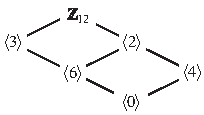
\includegraphics[width=0.280\linewidth,height=.8\textheight,keepaspectratio]{assets/p421_01.pdf}\end{center}
\end{BookFloat}

\BookExercise{33.}{8}

\begin{center}\begin{adjustbox}{max width=\linewidth}\BookInline{\displaystyle \langle 2\rangle}\end{adjustbox}\end{center}

\BookInline{\langle 4\rangle }

\BookInline{\langle 0\rangle }

\BookExercise{1.}{\textbf{4. a} \BookInline{T} \textbf{c}\BookInline{.F} \textbf{e}\BookInline{.T} \textbf{g}\BookInline{.F} \textbf{i}\BookInline{.T}}

\BookExercise{43.}{\BookInline{<Q,\allowbreak + >}}

\BookExercise{45.}{ There is none.}

\BookInline{\textstyle { \frac { \sqrt { 2 } } { 2 } } ( \pm 1 \pm i )}

\BookExercise{47.}{\BookInline{i,\allowbreak - i}}

\BookExercise{49.}{\BookInline{\textstyle { \frac { \sqrt { 2 } } { 2 } } ( \pm 1 \pm i )}}

\BookExercise{63.}{\BookInline{(p- 1)p^{r- 1}}}

\BookSectionTitle{7}{Generating Sets and Cayley Digraphs}

\BookExercise{3.}{\BookInline{\mathbb{Z}} 25}

\BookExercise{5.}{\BookInline{\cdots,\allowbreak - 24,\allowbreak - 18,\allowbreak - 12,\allowbreak - 6,\allowbreak 0,\allowbreak 6,\allowbreak 12,\allowbreak 18,\allowbreak 24,\allowbreak \cdots }}

\BookExercise{7.}{\BookInline{\{\iota,\allowbreak \rho ^{2},\allowbreak \rho ^{4},\allowbreak \rho ^{6},\allowbreak \mu,\allowbreak \mu \rho ^{2},\allowbreak \mu \rho ^{4},\allowbreak \mu \rho ^{6}\}}}

\BookExercise{9.}{\textbf{. a} \BookInline{c} \textbf{b}\BookInline{.e} \textbf{c}\BookInline{.d}}

\begin{BookFloat}{answers-p421-22}
\begin{center}\begin{adjustbox}{max width=\linewidth}
\renewcommand{\arraystretch}{1.2}\setlength{\tabcolsep}{5pt}
\begin{tabular}{c|c|c|c|c|c|c}
 & \BookInline{e} & \BookInline{a} & \BookInline{b} & \BookInline{c} & \BookInline{d} & \BookInline{f}\\\hline
\BookInline{e} & \BookInline{e} & \BookInline{a} & \BookInline{b} & \BookInline{c} & \BookInline{d} & \BookInline{f}\\\hline
\BookInline{a} & \BookInline{a} & \BookInline{e} & \BookInline{c} & \BookInline{b} & \BookInline{f} & \BookInline{d}\\\hline
\BookInline{b} & \BookInline{b} & \BookInline{d} & \BookInline{e} & \BookInline{f} & \BookInline{a} & \BookInline{c}\\\hline
\BookInline{c} & \BookInline{c} & \BookInline{f} & \BookInline{a} & \BookInline{d} & \BookInline{e} & \BookInline{b}\\\hline
\BookInline{d} & \BookInline{d} & \BookInline{b} & \BookInline{f} & \BookInline{e} & \BookInline{c} & \BookInline{a}\\\hline
\BookInline{f} & \BookInline{f} & \BookInline{c} & \BookInline{d} & \BookInline{a} & \BookInline{b} & \BookInline{e}\\
\end{tabular}
\end{adjustbox}\end{center}
\end{BookFloat}

\BookExercise{13.}{Choose a pair of generating directed arcs, call them\textit{ arc1} and\textit{ arc2}, start at any vertex of the digraph, and see if the sequences\textit{ arc1},\textit{ arc2} and\textit{ arc2},\textit{ arc1} lead to the same vertex. (This corresponds to asking if the two corresponding group generators commute.) The group is commutative if and only if these two sequences lead to the same vertex for \textit{every pair} of generating directed arcs.}

\BookExercise{15.}{It is not obvious, since a digraph of a cyclic group might be formed using a generating set of two or more elements, no one of which generates the group.}

\begin{BookFloat}{answers-p421-25}
\begin{center}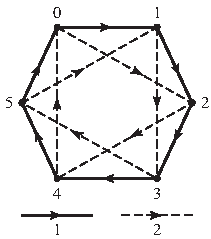
\includegraphics[width=0.289\linewidth,height=.8\textheight,keepaspectratio]{assets/p421_19.pdf}\end{center}
\end{BookFloat}

\BookExercise{9.}{\textbf{1. a} Starting from any vertex \BookInline{a,\allowbreak } every path through the graph that terminates at that same vertex \BookInline{a} represents a product of generators or their inverses that is equal to the identity and thus gives a relation.}

\BookExercise{b.}{\textbf{b}\BookInline{.a^{4}= e,\allowbreak b^{2}= e,\allowbreak (ab)^{2}= e}}

\end{BookBody}

% Source PDF page 422; original printed page 405
\BookSource{422}{405}
\BookNarrativefalse

\begin{BookBody}

\BookSectionTitle{8}{Groups of Permutations}

\BookExercise{3.}{Homomorphism}

\BookExercise{5.}{Not a homomorphism}

\BookExercise{7.}{Homomorphism}

\BookExercise{9.}{Not a homomorphism}

\BookExercise{11.}{Ker\BookInline{(\phi )= \langle 4\rangle.}}

\BookExercise{13.}{Ker\BookInline{(\phi )= \langle (5,\allowbreak 3)\rangle.}}

\BookExercise{15.}{\BookInline{\{0,\allowbreak 0\}}}

\BookExercise{17.}{\BookInline{\{1,\allowbreak 2,\allowbreak 5\},\allowbreak \{3\},\allowbreak \{4,\allowbreak 6\}}}

\BookExercise{19.}{\BookInline{\{1,\allowbreak 2,\allowbreak 3,\allowbreak 4,\allowbreak 5\},\allowbreak \{6\},\allowbreak \{7,\allowbreak 8\}}}

\BookExercise{21.}{\BookInline{\{2n\mid n\in \mathbb{Z}\},\allowbreak \{2n+ 1\mid n\in \mathbb{Z}\}}}

\BookExercise{23.}{\BookInline{(1,\allowbreak 8)(3,\allowbreak 6,\allowbreak 4)(5,\allowbreak 7)= (1,\allowbreak 8)(3,\allowbreak 4)(3,\allowbreak 6)(5,\allowbreak 7)}}

\BookExercise{25.}{\BookInline{(1,\allowbreak 5,\allowbreak 4,\allowbreak 8)(2,\allowbreak 3)(6,\allowbreak 7)= (1,\allowbreak 8)(1,\allowbreak 4)(1,\allowbreak 5)(2,\allowbreak 3)(6,\allowbreak 7)}}

\BookExercise{1.}{\textbf{3. a} \BookInline{F} \textbf{c}\BookInline{.F} \textbf{e}\BookInline{.F} \textbf{g}\BookInline{.T} \textbf{i}\BookInline{.T} \textbf{k}\BookInline{.T}}

\BookSectionTitle{9}{Finitely Generated Abelian Groups}

\begin{BookFloat}{answers-p422-17}
\noindent\textbf{1.}\quad
\begin{tabular}{cc|cc}
\textit{Element}&\textit{Order}&\textit{Element}&\textit{Order}\\
$(0,0)$&1&$(0,2)$&2\\
$(1,0)$&2&$(1,2)$&2\\
$(0,1)$&4&$(0,3)$&4\\
$(1,1)$&4&$(1,3)$&4
\end{tabular}
\end{BookFloat}

The group is not cyclic

\BookExercise{3.}{2}

\BookExercise{5.}{9}

\BookExercise{7.}{60}

\BookExercise{9.}{\BookInline{\{(0,\allowbreak 0),\allowbreak (0,\allowbreak 1)\},\allowbreak \{(0,\allowbreak 0),\allowbreak (1,\allowbreak 0)\},\allowbreak \{(0,\allowbreak 0),\allowbreak (1,\allowbreak 1)\}}}

\BookExercise{11.}{\BookInline{\{(0,\allowbreak 0),\allowbreak (0,\allowbreak 1),\allowbreak (0,\allowbreak 2),\allowbreak (0,\allowbreak 3)\}} \BookInline{\{(0,\allowbreak 0),\allowbreak (0,\allowbreak 2),\allowbreak (1,\allowbreak 0),\allowbreak (1,\allowbreak 2)\}} \BookInline{\{(0,\allowbreak 0),\allowbreak (1,\allowbreak 1),\allowbreak (0,\allowbreak 2),\allowbreak (1,\allowbreak 3)\}}}

\BookExercise{13.}{\BookInline{\mathbb{Z}_{20}\times \mathbb{Z}_{3},\allowbreak \mathbb{Z}_{15}\times \mathbb{Z}_{4},\allowbreak \mathbb{Z}_{12}\times \mathbb{Z}_{5},\allowbreak \mathbb{Z}_{5}\times \mathbb{Z}_{3}\times \mathbb{Z}_{4}}}

\BookExercise{15.}{12}

\BookExercise{17.}{168}

\BookExercise{19.}{180}

\BookExercise{21.}{\BookInline{\mathbb{Z}_{8},\allowbreak \mathbb{Z}_{2}\times \mathbb{Z}_{4},\allowbreak \mathbb{Z}_{2}\times \mathbb{Z}_{2}\times \mathbb{Z}_{2}}}

\BookExercise{23.}{\BookInline{\mathbb{Z}_{32},\allowbreak \mathbb{Z}_{2}\times \mathbb{Z}_{16},\allowbreak \mathbb{Z}_{4}\times \mathbb{Z}_{8},\allowbreak \mathbb{Z}_{2}\times \mathbb{Z}_{2}\times \mathbb{Z}_{8},\allowbreak \mathbb{Z}_{2}\times \mathbb{Z}_{4}\times \mathbb{Z}_{4},\allowbreak }}

\begin{center}\begin{adjustbox}{max width=\linewidth}\BookInline{\displaystyle \mathbb{Z}_{2}\times \mathbb{Z}_{2}\times \mathbb{Z}_{2}\times \mathbb{Z}_{4},\allowbreak \mathbb{Z}_{2}\times \mathbb{Z}_{2}\times \mathbb{Z}_{2}\times \mathbb{Z}_{2}\times \mathbb{Z}_{2}}\end{adjustbox}\end{center}

\BookExercise{25.}{\BookInline{\mathbb{Z}_{9}\times \mathbb{Z}_{121},\allowbreak \mathbb{Z}_{3}\times \mathbb{Z}_{3}\times \mathbb{Z}_{121},\allowbreak \mathbb{Z}_{9}\times \mathbb{Z}_{11}\times \mathbb{Z}_{11},\allowbreak \mathbb{Z}_{3}\times \mathbb{Z}_{3}\times \mathbb{Z}_{11}\times \mathbb{Z}_{11}}}

\begin{BookFloat}{answers-p422-32}
\BookExercise{29. a.}{\begin{tabular}{r|ccccccc}
$n$&2&3&4&5&6&7&8\\\hline
number of groups&2&3&5&7&11&15&22
\end{tabular}}
\end{BookFloat}

\BookExercise{b.}{\textbf{b. i)} 225 \textbf{ii)} 225 \textbf{iii)} 110}

\BookExercise{1.}{\textbf{3. a} It is abelian when the arrows on both \BookInline{n-}gons have the same (clockwise or counterclockwise) direction. \textbf{b}\BookInline{.\mathbb{Z}_{2}\times \mathbb{Z}_{n}} \textbf{c.} When \BookInline{n} is odd. \textbf{d.} The dihedral group \BookInline{D_{n}.}}

\BookExercise{33.}{\BookInline{\mathbb{Z}_{2}} is an example.}

\BookExercise{35.}{\BookInline{S_{3}} is an example.}

\BookExercise{37.}{The numbers are the same.}

\BookExercise{41.}{\BookInline{\{- 1,\allowbreak 1\}}}

\end{BookBody}

% Source PDF page 423; original printed page 406
\BookSource{423}{406}
\BookNarrativefalse

\begin{BookBody}

\BookSectionTitle{10}{Cosets and the Theorem of Lagrange}

\begin{center}\begin{adjustbox}{max width=\linewidth}\BookInline{\displaystyle 1+ 4\mathbb{Z}= \{\cdots ,\allowbreak - 7,\allowbreak - 3,\allowbreak 1,\allowbreak 5,\allowbreak 9,\allowbreak \cdots \}}\end{adjustbox}\end{center}

\begin{center}\begin{adjustbox}{max width=\linewidth}\BookInline{\displaystyle 2+ 4\mathbb{Z}= \{\cdots ,\allowbreak - 6,\allowbreak - 2,\allowbreak 2,\allowbreak 6,\allowbreak 10,\allowbreak \cdots \}}\end{adjustbox}\end{center}

\begin{center}\begin{adjustbox}{max width=\linewidth}\BookInline{\displaystyle 3+ 4\mathbb{Z}= \{\cdots ,\allowbreak - 5,\allowbreak - 1,\allowbreak 3,\allowbreak 7,\allowbreak 11,\allowbreak \cdots \}}\end{adjustbox}\end{center}

\BookExercise{3.}{\BookInline{\{0,\allowbreak 3,\allowbreak 6,\allowbreak 9,\allowbreak 12,\allowbreak 15\},\allowbreak \{1,\allowbreak 4,\allowbreak 7,\allowbreak 10,\allowbreak 13,\allowbreak 16\},\allowbreak \{2,\allowbreak 5,\allowbreak 8,\allowbreak 11,\allowbreak 14,\allowbreak 17\}}}

\BookExercise{5.}{\BookInline{\langle 18\rangle = \{0,\allowbreak 18\},\allowbreak 1+ \langle 18\rangle = \{1,\allowbreak 19\},\allowbreak 2+ \langle 18\rangle = \{2,\allowbreak 20\},\allowbreak \cdots,\allowbreak 17+ \langle 18\rangle = \{17,\allowbreak 35\}}}

\BookExercise{7.}{\BookInline{\{\iota,\allowbreak \mu \rho \},\allowbreak \{\rho,\allowbreak \mu \rho ^{2}\},\allowbreak \{\rho ^{2},\allowbreak \mu \rho ^{3}\},\allowbreak \{\rho ^{3},\allowbreak \mu \}} They are different.}

\BookExercise{9.}{\BookInline{\{\iota,\allowbreak \rho ^{2}\},\allowbreak \{\rho,\allowbreak \rho ^{3}\},\allowbreak \{\mu,\allowbreak \mu \rho ^{2}\},\allowbreak \{\mu \rho,\allowbreak \mu \rho ^{3}\}}}

\BookExercise{11.}{4}

\BookExercise{13.}{12}

\BookExercise{15.}{24}

\BookExercise{21.}{\BookInline{2\mathbb{Z}\leq \mathbb{Z}} has only 2 cosets.}

\BookExercise{23.}{\BookInline{G= \mathbb{Z}_{2},\allowbreak } subgroup \BookInline{H= \mathbb{Z}_{2}.}}

\BookExercise{25.}{Impossible. The number of cells must divide the order of the group, and 12 does not divide 6.}

\BookSectionTitle{11}{Plane Isometries}

\BookExercise{1.}{\textbf{. a} The only isometries of \BookInline{\mathbb{R}} leaving a number \BookInline{c} fixed are the reflection through \BookInline{c} that carries \BookInline{c+ x} to \BookInline{c- x} for all \BookInline{x\in \mathbb{R},\allowbreak } and the identity map.}

\BookExercise{b.}{The isometries of \BookInline{\mathbb{R}^{2}} that leave a point \BookInline{P} fixed are the rotations about \BookInline{P} through any angle \BookInline{\theta } where \BookInline{0\leq \theta <360^{\circ }} and the reflections across any axis that passes through \BookInline{P.}}

\BookExercise{c.}{The only isometries of \BookInline{\mathbb{R}} that carry a line segment into itself are the reflection through the midpoint of the line segment (see the answer to part (a)) and the identity map.}

\BookExercise{d.}{The isometries of \BookInline{\mathbb{R}^{2}} that carry a line segment into itself are a rotation of \BookInline{180^{\circ }} about the midpoint of the line segment, a reflection in the axis containing the line segment, a reflection in the axis perpendicular to the line segment at its midpoint, and the identity map.}

\BookExercise{e.}{The isometries of \BookInline{\mathbb{R}^{3}} that carry a line segment into itself include rotations through any angle about an axis that contains the line segment, reflections across any plane that contains the line segment, and reflection across the plane perpendicular to the line segment at its midpoint.}

\begin{BookFloat}{answers-p423-23}
\begin{center}\begin{adjustbox}{max width=\linewidth}
\renewcommand{\arraystretch}{1.2}\setlength{\tabcolsep}{5pt}
\begin{tabular}{c|c|c|c|c}
 & \BookInline{\tau } & \BookInline{\rho } & \BookInline{\mu } & \BookInline{\gamma }\\\hline
\BookInline{\tau } & \BookInline{\tau } & \BookInline{\rho } & \BookInline{\mu \gamma } & \BookInline{\mu \gamma }\\\hline
\BookInline{\rho } & \BookInline{\rho } & \BookInline{\rho \tau } & \BookInline{\mu \gamma } & \BookInline{\mu \gamma }\\\hline
\BookInline{\mu } & \BookInline{\mu \gamma } & \BookInline{\mu \gamma } & \BookInline{\tau \rho } & \BookInline{\tau \rho }\\\hline
\BookInline{\gamma } & \BookInline{\mu \gamma } & \BookInline{\mu \gamma } & \BookInline{\tau \rho } & \BookInline{\tau \rho }\\
\end{tabular}
\end{adjustbox}\end{center}
\end{BookFloat}

\begin{BookFloat}{answers-p423-24}
\begin{center}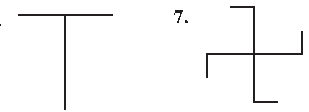
\includegraphics[width=0.424\linewidth,height=.8\textheight,keepaspectratio]{assets/p423_23.pdf}\end{center}
\end{BookFloat}

\BookExercise{9.}{\textit{Translation:} order \BookInline{\infty }}

\textit{Rotation:} order any \BookInline{n\geq 2} or \BookInline{\infty }

\textit{Reflection:} order 2

\textit{Glide reflection:} order \BookInline{\infty }

\BookExercise{11.}{Rotations}

\BookExercise{13.}{Only the identity and reflections.}

\BookExercise{17.}{Yes. The product of two translations is a translation and the inverse of a translation is a translation.}

\BookExercise{19.}{Yes. There is only one reflection \BookInline{\mu } across one particular line \BookInline{L,\allowbreak } and \BookInline{\mu ^{2}} is the identity, so we have a group isomorphic to \BookInline{\mathbb{Z}_{2}.}}

\end{BookBody}

% Source PDF page 424; original printed page 407
\BookSource{424}{407}
\BookNarrativefalse

\begin{BookBody}

\BookExercise{21.}{Only reflections and rotations (and the identity) because translations and glide reflections do not have finite order in the group of all plane isometries.}

\BookExercise{5.}{\textbf{2. a} No \textbf{b.} No \textbf{c.} Yes \textbf{d.} No \textbf{e}\BookInline{.D_{\infty }}}

\BookExercise{7.}{\textbf{2. a} Yes \textbf{b.} No \textbf{c.} No \textbf{d.} No \textbf{e}\BookInline{.D_{\infty }}}

\BookExercise{9.}{\textbf{2. a} No \textbf{b.} No \textbf{c.} No \textbf{d.} Yes \textbf{e}\BookInline{.\mathbb{Z}}}

\BookExercise{1.}{\textbf{3. a} Yes\BookInline{.90^{\circ },\allowbreak 180^{\circ }} \textbf{b.} Yes \textbf{c.} No}

\BookExercise{3.}{\textbf{3. a} No \textbf{b.} No \textbf{c.} No}

\BookExercise{5.}{\textbf{3. a} Yes\BookInline{.180^{\circ }} \textbf{b.} Yes \textbf{c.} No}

\BookExercise{7.}{\textbf{3. a} Yes\BookInline{.120^{\circ }} \textbf{b.} Yes \textbf{c.} No}

\BookExercise{9.}{\textbf{3. a} Yes\BookInline{.120^{\circ }} \textbf{b.} No \textbf{c.} No \textbf{d}\BookInline{.(1,\allowbreak 0),\allowbreak (1,\allowbreak \sqrt{3})}}

\BookSectionTitle{12}{Factor Groups}

\BookExercise{3.}{4}

\BookExercise{5.}{3}

\BookExercise{7.}{1}

\BookExercise{9.}{4}

\BookExercise{11.}{3}

\BookExercise{13.}{5}

\BookExercise{15.}{1}

\BookExercise{1.}{\textbf{2. a} When working with a factor group \BookInline{G/H,\allowbreak } you would let \BookInline{a} and \BookInline{b} be elements of \BookInline{G,\allowbreak } not elements of \BookInline{G/H.} The student probably does not understand what elements of \BookInline{G/H} look like and can write nothing sensible concerning them.}

\BookExercise{b.}{We must show that \BookInline{G/H} is abelian. Let \BookInline{aH} and \BookInline{bH} be two elements of \BookInline{G/H.}}

\BookExercise{3.}{\textbf{2. a} \BookInline{T} \textbf{c}\BookInline{.T} \textbf{e}\BookInline{.T} \textbf{g}\BookInline{.T} \textbf{i}\BookInline{.T}}

\BookExercise{35.}{Example: Let \BookInline{G= N= S_{3},\allowbreak } and let \BookInline{H= \{\rho _{0},\allowbreak \mu _{1}\}.} Then \BookInline{N} is normal in \BookInline{G,\allowbreak } but \BookInline{H\cap N= H} is not normal in \BookInline{G.}}

\BookSectionTitle{13}{Factor-Group Computations and Simple Groups}

\BookExercise{3.}{\BookInline{\mathbb{Z}_{4}}}

\BookExercise{5.}{\BookInline{\mathbb{Z}_{4}\times \mathbb{Z}_{8}}}

\BookExercise{7.}{\BookInline{\mathbb{Z}\times \mathbb{Z}_{2}}}

\BookExercise{9.}{\BookInline{\mathbb{Z}_{3}\times \mathbb{Z}\times \mathbb{Z}_{4}}}

\BookExercise{11.}{\BookInline{\mathbb{Z}_{2}\times \mathbb{Z}}}

\BookExercise{13.}{\BookInline{\mathbb{Z}\times \mathbb{Z}_{2}}}

\BookExercise{15.}{\BookInline{Z(D_{4})= C= \{\iota,\allowbreak \rho ^{2}\}}}

\BookExercise{17.}{\BookInline{Z(S_{3}\times D_{4})= \{\{\iota,\allowbreak \iota \},\allowbreak \{\iota,\allowbreak \rho \}\},\allowbreak C= A_{3}\times \{\iota,\allowbreak \rho \}.}}

\BookExercise{1.}{\textbf{2. a} \BookInline{T} \textbf{c}\BookInline{.F} \textbf{e}\BookInline{.F} \textbf{g}\BookInline{.F} \textbf{i}\BookInline{.T}}

\BookExercise{23.}{\BookInline{\{f\in F^{\ast }\mid f(0)= 1\}}}

\BookExercise{25.}{Yes. Let \BookInline{f(x)= 1} for \BookInline{x\geq 0} and \BookInline{f(x)= - 1} for \BookInline{x<0.} Then \BookInline{f(x)\cdot f(x)= 1} for all \BookInline{x,\allowbreak } so \BookInline{f^{2}\in K^{\ast }} but \BookInline{f} is not in \BookInline{K^{\ast }.} Thus \BookInline{fK^{\ast }} has order 2 in \BookInline{F^{\ast }/K^{\ast }.}}

\BookExercise{27.}{\BookInline{U}}

\BookExercise{29.}{The multiplicative group \BookInline{U} of complex numbers of absolute value 1}

\BookExercise{31.}{Let \BookInline{G= \mathbb{Z}_{2}\times \mathbb{Z}_{4}.} Then \BookInline{H= \langle (1,\allowbreak 0)\rangle } is isomorphic to \BookInline{K= \langle (0,\allowbreak 2)\rangle,\allowbreak } but \BookInline{G/H} is isomorphic to \BookInline{\mathbb{Z}_{4}} while \BookInline{G/K} is isomorphic to \BookInline{\mathbb{Z}_{2}\times \mathbb{Z}_{2}.}}

\BookExercise{3.}{\textbf{3. a} \BookInline{\{e\}} \textbf{b.} The whole group}

\BookSectionTitle{14}{Group Action on a Set}

\BookExercise{1.}{\BookInline{X_{\iota }= X,\allowbreak X_{\rho }= \{C\},\allowbreak X_{\rho }= \{m_{1},\allowbreak m_{2},\allowbreak d_{1},\allowbreak d_{2},\allowbreak C\},\allowbreak X_{\rho ^{3}}= \{C\},\allowbreak }}

\BookInline{X_{\mu _{\rho }}= \{s_{1},\allowbreak s_{3},\allowbreak m_{1},\allowbreak m_{2},\allowbreak C,\allowbreak P_{1},\allowbreak P_{3}\},\allowbreak X_{\mu \rho ^{3}}= \{s_{2},\allowbreak s_{0},\allowbreak m_{1},\allowbreak m_{2},\allowbreak C,\allowbreak P_{2},\allowbreak P_{0}\},\allowbreak } \BookInline{X_{\mu }= \{2,\allowbreak 0,\allowbreak d_{1},\allowbreak d_{2},\allowbreak C\},\allowbreak X_{\mu \rho ^{2}}= \{1,\allowbreak 3,\allowbreak d_{1},\allowbreak d_{2},\allowbreak C\}.}

\BookExercise{3.}{\BookInline{\{1,\allowbreak 2,\allowbreak 3,\allowbreak 0\},\allowbreak \{s_{1},\allowbreak s_{2},\allowbreak s_{3},\allowbreak s_{0}\},\allowbreak \{m_{1},\allowbreak m_{2}\},\allowbreak \{d_{1},\allowbreak d_{2}\},\allowbreak \{C\},\allowbreak \{P_{1},\allowbreak P_{2},\allowbreak P_{3},\allowbreak P_{0}\}}}

\BookExercise{5.}{\BookInline{\{\iota \}}}

\BookExercise{7.}{There are three orbits\BookInline{:\{\langle \mu \rangle,\allowbreak \langle \mu \rho ^{2}\rangle \},\allowbreak \{\langle \mu \rho \rangle,\allowbreak \langle \mu \rho ^{3}\rangle \},\allowbreak \{\langle \rho ^{2}\rangle \}}}

\BookExercise{9.}{3, 3; 3, 1, 1, 1; 1, 1, 1, 1, 1, 1}

\BookExercise{11.}{8, 2; 8, 1, 1; 4, 4, 2; 4, 4, 1, 1; 4, 2, 2, 2; 4, 2, 2, 1, 1; 4, 2, 1, 1, 1, 1; 4, 1, 1, 1, 1, 1, 1; 2, 2, 2, 2, 2; 2, 2, 2, 2, 1, 1; 2, 2, 2, 1, 1, 1, 1; 2, 2, 1, 1, 1, 1, 1, 1; 2, 1, 1, 1, 1, 1, 1, 1, 1; 1, 1, 1, 1, 1, 1, 1, 1, 1, 1}

\BookExercise{15.}{A transitive \BookInline{G-}set has just one orbit.}

\BookExercise{7.}{\textbf{1. a} \BookInline{\{s_{1},\allowbreak s_{2},\allowbreak s_{3},\allowbreak s_{0}\}} and \BookInline{\{P_{1},\allowbreak P_{2},\allowbreak P_{3},\allowbreak P_{0}\}}}

\BookExercise{1.}{\textbf{2. b} The set of points on the circle with center at the origin and passing through \BookInline{P} \textbf{c.} The cyclic subgroup \BookInline{\langle 2\pi \rangle } of \BookInline{G= \mathbb{R}}}

\end{BookBody}

% Source PDF page 425; original printed page 408
\BookSource{425}{408}
\BookNarrativefalse

\begin{BookBody}

\BookExercise{5.}{\textbf{2. a} \BookInline{K= g_{0}Hg_{0}^{- 1}.}}

\BookExercise{b.}{\textit{ Conjecture}\BookInline{:H} and \BookInline{K} should be conjugate subgroups of \BookInline{G.}}

\begin{BookFloat}{answers-p425-3}
\begin{center}\begin{adjustbox}{max width=\linewidth}
\renewcommand{\arraystretch}{1.2}\setlength{\tabcolsep}{5pt}
\begin{tabular}{c|c|c|c|c|c|c}
 & \BookInline{X} & \BookInline{Y} &  &  & \BookInline{Z} & \\
 & \BookInline{a} & \BookInline{a} & \BookInline{b} & \BookInline{a} & \BookInline{b} & \BookInline{c}\\\hline
0 & \BookInline{a} & \BookInline{a} & \BookInline{b} & \BookInline{a} & \BookInline{b} & \BookInline{c}\\\hline
1 & \BookInline{a} & \BookInline{b} & \BookInline{a} & \BookInline{b} & \BookInline{c} & \BookInline{a}\\\hline
2 & \BookInline{a} & \BookInline{a} & \BookInline{b} & \BookInline{c} & \BookInline{a} & \BookInline{b}\\\hline
3 & \BookInline{a} & \BookInline{b} & \BookInline{a} & \BookInline{a} & \BookInline{b} & \BookInline{c}\\\hline
4 & \BookInline{a} & \BookInline{a} & \BookInline{b} & \BookInline{b} & \BookInline{c} & \BookInline{a}\\\hline
5 & \BookInline{a} & \BookInline{b} & \BookInline{a} & \BookInline{c} & \BookInline{a} & \BookInline{b}\\
\end{tabular}
\end{adjustbox}\end{center}
\end{BookFloat}

\BookExercise{27.}{There are four of them\BookInline{:X,\allowbreak Y,\allowbreak Z,\allowbreak } and \BookInline{\mathbb{Z}_{6}.}}

\BookSectionTitle{15}{Applications of G-Sets to Counting}

\BookExercise{3.}{2}

\BookExercise{5.}{11,712}

\BookExercise{7.}{\textbf{. a} 45 \textbf{b.} 231}

\BookExercise{9.}{\textbf{. a} 90 \textbf{b.} 6,426}

\BookSectionTitle{16}{Isomorphism Theorems}

\BookExercise{1.}{\textbf{. a} \BookInline{K= \{0,\allowbreak 3,\allowbreak 6,\allowbreak 9\}.} \textbf{b}\BookInline{.0+ K= \{0,\allowbreak 3,\allowbreak 6,\allowbreak 9\},\allowbreak 1+ K= \{1,\allowbreak 4,\allowbreak 7,\allowbreak 10\},\allowbreak 2+ K= \{2,\allowbreak 5,\allowbreak 8,\allowbreak 11\}.} \textbf{c}\BookInline{.\mu (0+ K)= 0,\allowbreak \mu (1+ K)= 2,\allowbreak \mu (2+ K)= 1.}}

\BookExercise{3.}{\textbf{. a} \BookInline{HN= \{0,\allowbreak 2,\allowbreak 4,\allowbreak 6,\allowbreak 8,\allowbreak 10,\allowbreak 12,\allowbreak 14,\allowbreak 16,\allowbreak 18,\allowbreak 20,\allowbreak 22\},\allowbreak H\cap N= \{0,\allowbreak 12\}.} \textbf{b}\BookInline{.0+ N= \{0,\allowbreak 6,\allowbreak 12,\allowbreak 18\},\allowbreak 2+ N= \{2,\allowbreak 8,\allowbreak 14,\allowbreak 20\},\allowbreak 4+ N= \{4,\allowbreak 10,\allowbreak 16,\allowbreak 22\}.} \textbf{c}\BookInline{.0+ (H\cap N)= \{0,\allowbreak 12\},\allowbreak 4+ (H\cap N)= \{4,\allowbreak 16\},\allowbreak 8+ (H\cap N)= \{8,\allowbreak 20\}.} \textbf{d}\BookInline{.\mu (0+ (H\cap N))= 0+ N= \{0,\allowbreak 6,\allowbreak 12,\allowbreak 18\},\allowbreak \mu (4+ (H\cap N))= 4+ N= \{4,\allowbreak 10,\allowbreak 16,\allowbreak 20\},\allowbreak } \BookInline{\mu (8+ (H\cap N))= 8+ N= \{2,\allowbreak 8,\allowbreak 13,\allowbreak 20\}.}}

\BookExercise{5.}{\textbf{. a} \BookInline{0+ H= \{0,\allowbreak 4,\allowbreak 8,\allowbreak 12,\allowbreak 16,\allowbreak 20\},\allowbreak 1+ H= \{1,\allowbreak 5,\allowbreak 9,\allowbreak 13,\allowbreak 17,\allowbreak 21\},\allowbreak } \BookInline{2+ H= \{2,\allowbreak 6,\allowbreak 10,\allowbreak 14,\allowbreak 18,\allowbreak 22\},\allowbreak 3+ H= \{3,\allowbreak 7,\allowbreak 11,\allowbreak 15,\allowbreak 19,\allowbreak 23\}.} \textbf{b}\BookInline{.0+ K= \{0,\allowbreak 8,\allowbreak 16\},\allowbreak 1+ K= \{1,\allowbreak 9,\allowbreak 17\},\allowbreak 2+ K= \{2,\allowbreak 10,\allowbreak 18\},\allowbreak } \BookInline{3+ K= \{3,\allowbreak 11,\allowbreak 19\},\allowbreak } \BookInline{4+ K= \{4,\allowbreak 12,\allowbreak 20\},\allowbreak 5+ K= \{5,\allowbreak 13,\allowbreak 21\},\allowbreak 6+ K= \{6,\allowbreak 14,\allowbreak 22\},\allowbreak } \BookInline{7+ K= \{7,\allowbreak 15,\allowbreak 23\}.}}

\BookExercise{c.}{\textbf{c}\BookInline{.0+ K= \{0,\allowbreak 8,\allowbreak 16\},\allowbreak 4+ K= \{4,\allowbreak 12,\allowbreak 20\}.}}

\BookExercise{d.}{\textbf{d}\BookInline{.(0+ K)+ (H/K)= H/K= \{0+ K,\allowbreak 4+ K\}= \{\{0,\allowbreak 8,\allowbreak 16\},\allowbreak 4,\allowbreak 12,\allowbreak 20\}\}}}

\BookInline{(1+ K)+ (H/K)= \{1+ K,\allowbreak 5+ K\}= \{\{1,\allowbreak 9,\allowbreak 17\},\allowbreak \{5,\allowbreak 13,\allowbreak 21\}\}}

\BookInline{(2+ K)+ (H/K)= \{2+ K,\allowbreak 6+ K\}= \{\{2,\allowbreak 10,\allowbreak 18\},\allowbreak \{6,\allowbreak 14,\allowbreak 22\}\}}

\begin{center}\begin{adjustbox}{max width=\linewidth}\BookInline{\displaystyle (3+ K)+ (H/K)= \{3+ K,\allowbreak 7+ K\}= \{\{3,\allowbreak 11,\allowbreak 19\},\allowbreak \{7,\allowbreak 15,\allowbreak 23\}\}.}\end{adjustbox}\end{center}

\BookExercise{e.}{\textbf{e}\BookInline{.\phi (\{\{0,\allowbreak 8,\allowbreak 16\},\allowbreak \{4,\allowbreak 12,\allowbreak 20\}\})= \{0,\allowbreak 4,\allowbreak 8,\allowbreak 12,\allowbreak 16,\allowbreak 20\},\allowbreak \phi (\{\{1,\allowbreak 9,\allowbreak 17\},\allowbreak \{5,\allowbreak 13,\allowbreak 21\}\})} \BookInline{= \{1,\allowbreak 5,\allowbreak 9,\allowbreak 13,\allowbreak 17,\allowbreak 21\},\allowbreak \phi (\{\{2,\allowbreak 10,\allowbreak 18\},\allowbreak \{6,\allowbreak 14,\allowbreak 22\}\})= \{2,\allowbreak 6,\allowbreak 10,\allowbreak 14,\allowbreak 18,\allowbreak 22\},\allowbreak } \BookInline{\phi (\{\{3,\allowbreak 11,\allowbreak 19\},\allowbreak \{7,\allowbreak 15,\allowbreak 23\}\})= \{3,\allowbreak 7,\allowbreak 11,\allowbreak 15,\allowbreak 19,\allowbreak 23\}}}

\BookSectionTitle{17}{Sylow Theorems}

\BookExercise{3.}{1, 3}

\BookExercise{5.}{The Sylow 3-subgroups are \BookInline{\langle (1,\allowbreak 2,\allowbreak 3)\rangle,\allowbreak \langle (1,\allowbreak 2,\allowbreak 4)\rangle,\allowbreak \langle (1,\allowbreak 3,\allowbreak 4)\rangle,\allowbreak } and \BookInline{\langle (2,\allowbreak 3,\allowbreak 4)\rangle.} Also \BookInline{(3,\allowbreak 4)\langle (1,\allowbreak 2,\allowbreak 3)\rangle (3,\allowbreak 4)= \langle (1,\allowbreak 2,\allowbreak 4)\rangle,\allowbreak } etc.}

\BookExercise{7.}{1, 2, 3, 4, 5, 7, 9, 11, 13, 15, 17, 19.}

\BookExercise{13.}{\textbf{13. a}\BookInline{.T} \textbf{c}\BookInline{.F} \textbf{e}\BookInline{.T} \textbf{g}\BookInline{.T} \textbf{i}\BookInline{.F}}

\end{BookBody}

% Source PDF page 426; original printed page 409
\BookSource{426}{409}
\BookNarrativefalse

\begin{BookBody}

\BookSectionTitle{18}{Series of Groups}

\BookExercise{1.}{The refinements \BookInline{\{0\}<250\mathbb{Z}<10\mathbb{Z}<\mathbb{Z}} of \BookInline{\{0\}<10\mathbb{Z}<\mathbb{Z}} and \BookInline{\{0\}<250\mathbb{Z}<25\mathbb{Z}<\mathbb{Z}} of \BookInline{0<25\mathbb{Z}<\mathbb{Z}} are isomorphic.}

\BookExercise{3.}{\BookInline{\{0\}<\langle 27\rangle <\langle 9\rangle <\mathbb{Z}_{54}} and \BookInline{\{0\}<\langle 18\rangle <\langle 2\rangle <\mathbb{Z}_{54}}}

\BookExercise{5.}{The refinements \BookInline{\{(0,\allowbreak 0)\}<(4800\mathbb{Z})\times \mathbb{Z}<(240\mathbb{Z})\times \mathbb{Z}<(60\mathbb{Z})\times \mathbb{Z}<(10\mathbb{Z})\times \mathbb{Z}<\mathbb{Z}\times \mathbb{Z}} of the first series and \BookInline{\{(0,\allowbreak 0)\}<\mathbb{Z}\times (4800\mathbb{Z})<\mathbb{Z}\times (480\mathbb{Z})<\mathbb{Z}\times (80\mathbb{Z})<\mathbb{Z}\times (20\mathbb{Z})<\mathbb{Z}\times \mathbb{Z}} of the second series are isomorphic refinements.}

\BookExercise{7.}{\BookInline{\{0\}<\langle 16\rangle <\langle 8\rangle <\langle 4\rangle <\langle 2\rangle <\mathbb{Z}_{48}}}

\BookInline{\{0\}<\langle 24\rangle <\langle 8\rangle <\langle 4\rangle <\langle 2\rangle <\mathbb{Z}_{48}}

\begin{center}\begin{adjustbox}{max width=\linewidth}\BookInline{\displaystyle \{0\}<\langle 24\rangle <\langle 12\rangle <\langle 4\rangle <\langle 2\rangle <\mathbb{Z}_{48}}\end{adjustbox}\end{center}

\begin{center}\begin{adjustbox}{max width=\linewidth}\BookInline{\displaystyle \{0\}<\langle 24\rangle <\langle 12\rangle <\langle 6\rangle <\langle 2\rangle <\mathbb{Z}_{48}}\end{adjustbox}\end{center}

\begin{center}\begin{adjustbox}{max width=\linewidth}\BookInline{\displaystyle \{0\}<\langle 24\rangle <\langle 12\rangle <\langle 6\rangle <\langle 3\rangle <\mathbb{Z}_{48}}\end{adjustbox}\end{center}

\BookExercise{9.}{\BookInline{\{(\iota,\allowbreak 0)\}<A_{3}\times \{0\}<S_{3}\times (0)<S_{3}\times \mathbb{Z}_{2}}}

\begin{center}\begin{adjustbox}{max width=\linewidth}\BookInline{\displaystyle \{(\iota ,\allowbreak 0)\}<\{\iota \}\times \mathbb{Z}_{2}<A_{3}\times \mathbb{Z}_{2}<S_{3}\times \mathbb{Z}_{2}}\end{adjustbox}\end{center}

\begin{center}\begin{adjustbox}{max width=\linewidth}\BookInline{\displaystyle \{(\iota ,\allowbreak 0)\}<A_{3}\times \{0\}<A_{3}\times \mathbb{Z}_{2}<S_{3}\times \mathbb{Z}_{2}}\end{adjustbox}\end{center}

\BookExercise{11.}{\BookInline{\{\iota \}\times \mathbb{Z}_{4}}}

\BookExercise{13.}{\BookInline{\{\iota \}\times \mathbb{Z}_{4}\leq \{\iota \}\times \mathbb{Z}_{4}\leq \{\iota \}\times \mathbb{Z}_{4}\leq \cdots.}}

\BookExercise{7.}{\textbf{1. a} \BookInline{T} \textbf{c}\BookInline{.T} \textbf{e}\BookInline{.F} \textbf{g}\BookInline{.F} \textbf{i}\BookInline{.T}}

\BookExercise{i.}{The Jordan-Ho¨lder theorem applied to the groups \BookInline{\mathbb{Z}_{n}} implies the Fundamental Theorem of Arithmetic.}

\BookExercise{19.}{Yes\BookInline{.\{\iota \}<\{\iota,\allowbreak \rho \}<\{\iota,\allowbreak \rho,\allowbreak \rho ^{2},\allowbreak \rho ^{3}\}<D_{4}} is a composition (actually a principal) series and all factor groups are isomorphic to \BookInline{\mathbb{Z}_{2}} and are thus abelian.}

\textit{Chain (4)}

\BookExercise{21.}{\textit{Chain (3)}}

\begin{center}\begin{adjustbox}{max width=\linewidth}\BookInline{\displaystyle \{0\}\leq \langle 12\rangle \leq \langle 12\rangle \leq \langle 12\rangle}\end{adjustbox}\end{center}

\begin{center}\begin{adjustbox}{max width=\linewidth}\BookInline{\displaystyle \{0\}\leq \langle 12\rangle <\langle 12\rangle \leq \langle 6\rangle}\end{adjustbox}\end{center}

\begin{center}\begin{adjustbox}{max width=\linewidth}\BookInline{\displaystyle \leq \langle 12\rangle \leq \langle 12\rangle \leq \langle 4\rangle}\end{adjustbox}\end{center}

\begin{center}\begin{adjustbox}{max width=\linewidth}\BookInline{\displaystyle \leq \langle 6\rangle \leq \langle 6\rangle \leq \langle 3\rangle}\end{adjustbox}\end{center}

\begin{center}\begin{adjustbox}{max width=\linewidth}\BookInline{\displaystyle \leq \langle 2\rangle \leq \mathbb{Z}_{24}\leq \mathbb{Z}_{24}}\end{adjustbox}\end{center}

\begin{center}\begin{adjustbox}{max width=\linewidth}\BookInline{\displaystyle \leq \langle 3\rangle \leq \mathbb{Z}_{24}\leq \mathbb{Z}_{24}}\end{adjustbox}\end{center}

\textit{Isomorphisms}

\begin{center}\begin{adjustbox}{max width=\linewidth}\BookInline{\displaystyle \langle 12\rangle /\{0\}\simeq \langle 12\rangle /\{0\}\simeq \mathbb{Z}_{2},\allowbreak \langle 12\rangle /\langle 12\rangle \simeq \langle 6\rangle /\langle 6\rangle \simeq \{0\},\allowbreak }\end{adjustbox}\end{center}

\begin{center}\begin{adjustbox}{max width=\linewidth}\BookInline{\displaystyle \langle 12\rangle /\langle 12\rangle \simeq \langle 3\rangle /\langle 3\rangle \simeq \{0\},\allowbreak \langle 12\rangle /\langle 12\rangle \simeq \langle 12\rangle /\langle 12\rangle \simeq \{0\},\allowbreak }\end{adjustbox}\end{center}

\begin{center}\begin{adjustbox}{max width=\linewidth}\BookInline{\displaystyle \langle 12\rangle /\langle 12\rangle \simeq \langle 6\rangle /\langle 6\rangle \simeq \{0\},\allowbreak \langle 4\rangle /\langle 12\rangle \simeq \mathbb{Z}_{24}/\langle 3\rangle \simeq \mathbb{Z}_{3}}\end{adjustbox}\end{center}

\begin{center}\begin{adjustbox}{max width=\linewidth}\BookInline{\displaystyle \langle 2\rangle /\langle 4\rangle \simeq \langle 6\rangle /\langle 12\rangle \simeq \mathbb{Z}_{2},\allowbreak \mathbb{Z}_{24}/\langle 2\rangle \simeq \langle 3\rangle /\langle 6\rangle \simeq \mathbb{Z}_{2}}\end{adjustbox}\end{center}

\begin{center}\begin{adjustbox}{max width=\linewidth}\BookInline{\displaystyle \mathbb{Z}_{24}/\mathbb{Z}_{24}\simeq \mathbb{Z}_{24}/\mathbb{Z}_{24}\simeq \{0\}}\end{adjustbox}\end{center}

\BookSectionTitle{19}{Free Abelian Groups}

\BookExercise{3.}{No\BookInline{.n(2,\allowbreak 1)+ m(4,\allowbreak 1)} can never yield an odd number for first coordinate.}

\BookExercise{7.}{\BookInline{2\mathbb{Z}<\mathbb{Z},\allowbreak } rank \BookInline{r= 1}}

\BookSectionTitle{20}{Free Groups}

\begin{center}\begin{adjustbox}{max width=\linewidth}\BookInline{\displaystyle 1.\mathrm{a}.a^{2}b^{2}a^{3}c^{3}b^{- 2},\allowbreak b^{2}c^{- 3}a^{- 3}b^{- 2}a^{- 2}\mathrm{b}.a^{- 1}b^{3}a^{4}c^{6}a^{- 1},\allowbreak ac^{- 6}a^{- 4}b^{- 3}a}\end{adjustbox}\end{center}

\BookExercise{3.}{\textbf{a.} 16 \textbf{b.} 36 \textbf{c.} 36}

\BookExercise{5.}{\textbf{a.} 16 \textbf{b.} 36 \textbf{c.} 18}

\BookExercise{1.}{\textbf{1. a}\textit{ Partial answer}\BookInline{:\{1\}} is a basis for \BookInline{\mathbb{Z}_{4}.} \textbf{c.} Yes}

\BookExercise{3.}{\textbf{1. c} A blop group on \BookInline{S} is isomorphic to the\textit{ free group} \BookInline{F[S]} on \BookInline{S.}}

\end{BookBody}

% Source PDF page 427; original printed page 410
\BookSource{427}{410}
\BookNarrativefalse

\begin{BookBody}

\BookSectionTitle{21}{Group Presentations}

\BookExercise{1.}{\BookInline{(a:a^{4}= 1);(a,\allowbreak b:a^{4}= 1,\allowbreak b= a^{2});(a,\allowbreak b,\allowbreak c:a= 1,\allowbreak b^{4}= 1,\allowbreak c= 1).(}Other answers are possible.)}

\BookTextHeading{\textbf{3.} \textit{Octic group:}  }

\begin{BookFloat}{answers-p427-3}
\begin{center}\begin{adjustbox}{max width=\linewidth}
\renewcommand{\arraystretch}{1.2}\setlength{\tabcolsep}{5pt}
\begin{tabular}{c|c|c|c|c|c|c|c|c}
 & 1 & \BookInline{a} & \BookInline{a^{2}} & \BookInline{a^{3}} & \BookInline{b} & \BookInline{ab} & \BookInline{a^{2}b} & \BookInline{a^{3}b}\\\hline
1 & 1 & \BookInline{a} & \BookInline{a^{2}} & \BookInline{a^{3}} & \BookInline{b} & \BookInline{ab} & \BookInline{a^{2}b} & \BookInline{a^{3}b}\\\hline
\BookInline{a} & \BookInline{a} & \BookInline{a^{2}} & \BookInline{a^{3}} & 1 & \BookInline{ab} & \BookInline{a^{2}b} & \BookInline{a^{3}b} & \BookInline{b}\\\hline
\BookInline{a^{2}} & \BookInline{a^{2}} & \BookInline{a^{3}} & 1 & \BookInline{a} & \BookInline{a^{2}b} & \BookInline{a^{3}b} & \BookInline{b} & \BookInline{ab}\\\hline
\BookInline{a^{3}} & \BookInline{a^{3}} & 1 & \BookInline{a} & \BookInline{a^{2}} & \BookInline{a^{3}b} & \BookInline{b} & \BookInline{ab} & \BookInline{a^{2}b}\\\hline
\BookInline{b} & \BookInline{b} & \BookInline{a^{3}b} & \BookInline{a^{2}b} & \BookInline{ab} & 1 & \BookInline{a^{3}} & \BookInline{a^{2}} & \BookInline{a}\\\hline
\BookInline{ab} & \BookInline{ab} & \BookInline{b} & \BookInline{a^{3}b} & \BookInline{a^{2}b} & \BookInline{a} & 1 & \BookInline{a^{3}} & \BookInline{a^{2}}\\\hline
\BookInline{a^{2}b} & \BookInline{a^{2}b} & \BookInline{ab} & \BookInline{b} & \BookInline{a^{3}b} & \BookInline{a^{2}} & \BookInline{a} & 1 & \BookInline{a^{3}}\\\hline
\BookInline{a^{3}b} & \BookInline{a^{3}b} & \BookInline{a^{2}b} & \BookInline{ab} & \BookInline{b} & \BookInline{a^{3}} & \BookInline{a^{2}} & \BookInline{a} & 1\\
\end{tabular}
\end{adjustbox}\end{center}
\end{BookFloat}

\textit{Quaternion group:} The same as the table for the octic group except that the 16 entries in the lower right corner are

\begin{BookFloat}{answers-p427-5}
\begin{center}\begin{adjustbox}{max width=\linewidth}
\renewcommand{\arraystretch}{1.2}\setlength{\tabcolsep}{5pt}
\begin{tabular}{c|c|c|c}
\BookInline{a^{2}} & \BookInline{a} & 1 & \BookInline{a^{3}}\\\hline
\BookInline{a^{3}} & \BookInline{a^{2}} & \BookInline{a} & 1\\\hline
1 & \BookInline{a^{3}} & \BookInline{a^{2}} & \BookInline{a}\\\hline
\BookInline{a} & 1 & \BookInline{a^{3}} & \BookInline{a^{2}}\\
\end{tabular}
\end{adjustbox}\end{center}
\end{BookFloat}

\BookExercise{5.}{\BookInline{\mathbb{Z}_{21}.(a,\allowbreak b:a^{7}= 1,\allowbreak b^{3}= 1,\allowbreak ba= a^{2}b)}}

\BookSectionTitle{22}{Rings and Fields}

\BookExercise{3.}{1}

\BookExercise{5.}{(1, 6)}

\BookExercise{7.}{Commutative ring, no unity, not a field}

\BookExercise{9.}{Commutative ring with unity, not a field}

\BookExercise{11.}{Commutative ring with unity, not a field}

\BookExercise{13.}{No\BookInline{.\{}\textit{ri}\BookInline{\mid r\in \mathbb{R}\}} is not closed under multiplication.}

\BookExercise{15.}{\BookInline{(1,\allowbreak 1),\allowbreak (1,\allowbreak - 1),\allowbreak (- 1,\allowbreak 1),\allowbreak (- 1,\allowbreak - 1)}}

\BookExercise{17.}{All nonzero \BookInline{q\in \mathbb{Q}}}

\BookExercise{19.}{1, 3}

\BookExercise{21.}{Let \BookInline{\mathbb{R}= \mathbb{Z}} with unity 1 and R\BookInline{\prime = \mathbb{Z}\times \mathbb{Z}} with unity \BookInline{1^{\prime }= (1,\allowbreak 1).} Let \BookInline{\phi:R\to R^{\prime }} be defined by \BookInline{\phi (n)= (n,\allowbreak 0).} Then \BookInline{\phi (1)= (1,\allowbreak 0)\neq 1^{\prime }.}}

\BookExercise{23.}{\BookInline{\phi _{1}:\mathbb{Z}\to \mathbb{Z}} where \BookInline{\phi _{1}(n)= 0,\allowbreak \phi _{2}:\mathbb{Z}\to \mathbb{Z}} where \BookInline{\phi _{2}(n)= n}}

\BookExercise{25.}{\BookInline{\phi _{1}:\mathbb{Z}\times \mathbb{Z}\to \mathbb{Z}} where \BookInline{\phi _{1}(n,\allowbreak m)= 0,\allowbreak \phi _{2}:\mathbb{Z}\times \mathbb{Z}\to \mathbb{Z}} where \BookInline{\phi _{2}(n,\allowbreak m)= n}}

\BookInline{\phi _{3}:\mathbb{Z}\times \mathbb{Z}\to \mathbb{Z}} where \BookInline{\phi _{3}(n,\allowbreak m)= m}

\BookExercise{27.}{The reasoning is not correct since a product \BookInline{(X- I_{3})(X+ I_{3})} of two matrices may be the zero matrix 0 without having either matrix be 0. Counterexample:}

\begin{center}\begin{adjustbox}{max width=\linewidth}\BookInline{\displaystyle \begin{bmatrix} 0 & 0 & 1 \\ 0 & 1 & 0 \\ 1 & 0 & 0 \end{bmatrix} ^ { 2 } = I _ { 3 } .}\end{adjustbox}\end{center}

\BookExercise{29.}{2,10. In the ring \BookInline{\mathbb{Z}_{14}} there are nonzero elements 2 and 7 which when multiplied give 0. This is not the case in \BookInline{\mathbb{Z}_{13}.}}

\BookExercise{33.}{\BookInline{a= 2,\allowbreak b= 3} in \BookInline{\mathbb{Z}_{6}}}

\BookExercise{5.}{\textbf{3. a} \BookInline{T} \textbf{c}\BookInline{.F} \textbf{e}\BookInline{.T} \textbf{g}\BookInline{.T} \textbf{i}\BookInline{.T}}

\end{BookBody}

% Source PDF page 428; original printed page 411
\BookSource{428}{411}
\BookNarrativefalse

\begin{BookBody}

\BookSectionTitle{23}{Integral Domains}

\BookExercise{3.}{No solutions}

\BookExercise{5.}{0}

\BookExercise{7.}{0}

\BookExercise{9.}{12}

\BookExercise{11.}{1, 5 are units; 2, 3, 4 are 0 divisors.}

\BookExercise{13.}{1, 2, 4, 7, 8, 11, 13, 14 are units; 3, 5, 6, 9, 10, 12 are 0 divisors.}

\BookExercise{15.}{(1, 1), (1, 2), (2, 1), (2, 2) are units; (0, 1), (0, 2), (1, 0), (2, 0) are 0 divisors.}

\BookExercise{17.}{\BookInline{a^{4}+ 2a^{2}b^{2}+ b^{4}}}

\BookExercise{19.}{\BookInline{a^{6}+ 2a^{3}b^{3}+ b^{6}}}

\BookExercise{3.}{\textbf{2. a} \BookInline{F} \textbf{c}\BookInline{.F} \textbf{e}\BookInline{.T} \textbf{g}\BookInline{.F} \textbf{i}\BookInline{.F}}

\BookExercise{1.}{Det\BookInline{(A)= 0.}}

\BookExercise{2.}{The column vectors of \BookInline{A} are dependent.}

\BookExercise{3.}{The row vectors of \BookInline{A} are dependent.}

\BookExercise{4.}{Zero is an eigenvalue of \BookInline{A.}}

\BookExercise{5.}{\BookInline{A} is not invertible.}

\BookSectionTitle{24}{Fermat’s and Euler’s Theorems}

\BookExercise{3.}{Any of 3, 5, 6, 7, 10, 11, 12, or 14.}

\BookExercise{5.}{2}

\BookExercise{7.}{\BookInline{\varphi (1)= 1\varphi (7)= 6\varphi (13)= 12\varphi (19)= 18\varphi (25)= 20}}

\BookInline{\varphi (2)= 1\varphi (8)= 4\varphi (14)= 6\varphi (20)= 8\varphi (26)= 12}

\BookInline{\varphi (3)= 2\varphi (9)= 6\varphi (15)= 8\varphi (21)= 12\varphi (27)= 18}

\BookInline{\varphi (4)= 2\varphi (10)= 4\varphi (16)= 8\varphi (22)= 10\varphi (28)= 12}

\BookInline{\varphi (5)= 4}

\BookInline{\varphi (11)= 10}

\BookInline{\varphi (17)= 16}

\BookInline{\varphi (23)= 22}

\BookInline{\varphi (29)= 28}

\BookInline{\varphi (6)= 2\varphi (12)= 4\varphi (18)= 6\varphi (24)= 8\varphi (30)= 8}

\BookExercise{9.}{\BookInline{(p- 1)(q- 1)}}

\BookExercise{11.}{\BookInline{1+ 4\mathbb{Z},\allowbreak 3+ 4\mathbb{Z}}}

\BookExercise{13.}{No solutions}

\BookExercise{15.}{No solutions}

\BookExercise{17.}{\BookInline{3+ 65\mathbb{Z},\allowbreak 16+ 65\mathbb{Z},\allowbreak 29+ 65\mathbb{Z},\allowbreak 42+ 65\mathbb{Z},\allowbreak 55+ 65\mathbb{Z}}}

\BookExercise{19.}{1}

\BookExercise{21.}{9}

\BookExercise{3.}{\textbf{2. a} \BookInline{F} \textbf{c}\BookInline{.T} \textbf{e}\BookInline{.T} \textbf{g}\BookInline{.F} \textbf{i}\BookInline{.F}}

\BookSectionTitle{25}{Encryption}

\BookExercise{3.}{\BookInline{n= pq= 33,\allowbreak (p- 1)(q- 1)= 20,\allowbreak } so the pairs are (3,7), (7,3), (9,9), (11,11), (13,17), (17,13)}

\BookExercise{5.}{\BookInline{s= 77}}

\BookExercise{7.}{\textbf{. a} \BookInline{y= 64} \textbf{b}\BookInline{.r= 13} \textbf{c}\BookInline{.64^{13}\equiv 25(}mod 143)}

\BookExercise{9.}{Private key is \BookInline{p= 257,\allowbreak q= 359,\allowbreak n= 92263,\allowbreak r= 1493.} Public key is \BookInline{n= 92263} and \BookInline{s= 9085.}}

\BookSectionTitle{26}{the Field of Quotients of an Integral Domain}

\BookExercise{15.}{It is isomorphic to the ring \BookInline{D} of all rational numbers that can be expressed as a quotient of integers with denominator some power of 2.}

\BookExercise{17.}{It runs into trouble when we try to prove the transitive property in the proof of Lemma 5.4.2, for multiplicative cancellation may not hold. For \BookInline{R= \mathbb{Z}_{6}} and \BookInline{T= \{1,\allowbreak 2,\allowbreak 4\}} we have \BookInline{(1,\allowbreak 2)\sim (2,\allowbreak 4)} since \BookInline{(1)(4)= (2)(2)= 4} and \BookInline{(2,\allowbreak 4)\sim (2,\allowbreak 1)} since \BookInline{(2)(1)= (4)(2)} in \BookInline{\mathbb{Z}_{6}.} However, (1, 2) is not equivalent to (2, 1) because \BookInline{(1)(1)\neq (2)(2)} in \BookInline{\mathbb{Z}_{6}.}}

\BookSectionTitle{27}{Rings of Polynomials}

\BookExercise{3.}{\BookInline{f(x)+ g(x)= 5x^{2}+ 5x+ 1,\allowbreak f(x)g(x)= x^{3}+ 5x}}

\BookExercise{5.}{16}

\BookExercise{7.}{7}

\BookExercise{9.}{2}

\BookExercise{11.}{0}

\BookExercise{13.}{2, 3}

\BookExercise{15.}{0, 2, 4}

\BookExercise{17.}{0, 1, 2, 3}

\BookExercise{21.}{\BookInline{0,\allowbreak x- 5,\allowbreak 2x- 10,\allowbreak x^{2}- 25,\allowbreak x^{2}- 5x,\allowbreak x^{4}- 5x^{3}.(}Other answers are possible.)}

\BookExercise{3.}{\textbf{2. a} \BookInline{T} \textbf{c}\BookInline{.T} \textbf{e}\BookInline{.F} \textbf{g}\BookInline{.T} \textbf{i}\BookInline{.T}}

\BookExercise{5.}{\textbf{2. a} They are the units of \BookInline{D.} \textbf{b}\BookInline{.1,\allowbreak - 1} \textbf{c.} 1, 2, 3, 4, 5, 6}

\BookExercise{7.}{\textbf{2. b} \BookInline{F} \textbf{c}\BookInline{.F[x]}}

\BookExercise{1.}{\textbf{3. a} 4, 27 \textbf{b}\BookInline{.\mathbb{Z}_{2}\times \mathbb{Z}_{2},\allowbreak \mathbb{Z}_{3}\times \mathbb{Z}_{3}\times \mathbb{Z}_{3}}}

\end{BookBody}

% Source PDF page 429; original printed page 412
\BookSource{429}{412}
\BookNarrativefalse

\begin{BookBody}

\BookSectionTitle{28}{Factorization of Polynomials over a Field}

\BookExercise{3.}{\BookInline{q(x)= 6x^{4}+ 7x^{3}+ 2x^{2}- x+ 2,\allowbreak r(x)= 4}}

\BookExercise{5.}{2, 3}

\BookExercise{7.}{3, 10, 5, 11, 14, 7, 12, 6}

\BookExercise{9.}{\BookInline{(x- 1)(x+ 1)(x- 2)(x+ 2)}}

\BookExercise{11.}{\BookInline{(x- 3)(x+ 3)(2x+ 3)}}

\BookExercise{13.}{Yes. It is of degree 3 with no zeros in \BookInline{\mathbb{Z}_{5}.}}

\begin{center}\begin{adjustbox}{max width=\linewidth}\BookInline{\displaystyle 2x^{3}+ x^{2}+ 2x+ 2}\end{adjustbox}\end{center}

\BookExercise{15.}{\textit{Partial answer}\BookInline{:g(x)} is irreducible over \BookInline{\mathbb{R},\allowbreak } but it is not irreducible over \BookInline{\mathbb{C}.}}

\BookExercise{19.}{Yes\BookInline{.p= 3}}

\BookExercise{21.}{Yes\BookInline{.p= 5}}

\BookExercise{5.}{\textbf{2. a} \BookInline{T} \textbf{c}\BookInline{.T} \textbf{e}\BookInline{.T} \textbf{g}\BookInline{.T} \textbf{i}\BookInline{.T}}

\BookExercise{27.}{\BookInline{x^{2}+ x+ 1}}

\BookExercise{29.}{\BookInline{x^{2}+ 1,\allowbreak x_{2}^{2}+ x+ 2,\allowbreak x^{2}+ 2x+ 2,\allowbreak 2x^{2}+ 2,\allowbreak 2x^{2}+ x+ 1,\allowbreak 2x^{2}+ 2x+ 1}}

\BookExercise{31.}{\BookInline{p(p- 1)/2}}

\BookSectionTitle{29}{Algebraic Coding Theory}

\BookExercise{3.}{5 \BookInline{\mathbb{Z}} 2}

\BookExercise{5.}{\textbf{. a} \BookInline{\{(0,\allowbreak 0)\},\allowbreak \{(0,\allowbreak 0),\allowbreak (1,\allowbreak 1)\},\allowbreak \mathbb{Z}_{2}^{2}} \textbf{b}\BookInline{.\{0,\allowbreak 0,\allowbreak 0\},\allowbreak \{(0,\allowbreak 0,\allowbreak 0),\allowbreak (1,\allowbreak 1,\allowbreak 1)\},\allowbreak \mathbb{Z}_{2}^{3}}}

\BookExercise{c.}{\textbf{c}\BookInline{.\{(0,\allowbreak 0,\allowbreak 0,\allowbreak 0)\},\allowbreak \{(0,\allowbreak 0,\allowbreak 0,\allowbreak 0),\allowbreak (1,\allowbreak 1,\allowbreak 1,\allowbreak 1)\},\allowbreak \{(0,\allowbreak 0,\allowbreak 0,\allowbreak 0),\allowbreak (0,\allowbreak 1,\allowbreak 0,\allowbreak 1),\allowbreak (1,\allowbreak 0,\allowbreak 1,\allowbreak 0),\allowbreak (1,\allowbreak 1,\allowbreak 1,\allowbreak 1)\},\allowbreak \mathbb{Z}_{2}^{4}}}

\BookExercise{7.}{\textbf{. a} \BookInline{x^{7}+ 1= (x^{3}+ x+ 1)(x^{4}+ x^{2}+ x+ 1)} \textbf{b}\BookInline{.C} consists of the cyclic shifts of \BookInline{x^{3}+ x+ 1,\allowbreak x^{4}+ x^{3}+ x^{2}+ 1} together with 0 and \BookInline{x^{6}+ x^{5}+ x^{4}+ x^{3}+ x^{2}+ x+ 1.} \textbf{c.} A single bit error can be detected and corrected. \textbf{d.} A two-bit error can be detected, but not corrected.}

\BookExercise{9.}{\textbf{. a} Use long division to verify that \BookInline{(x^{3}+ 1)(x^{6}+ x^{3}+ 1)= x^{9}+ 1.}}

\BookExercise{b.}{\textbf{b}\BookInline{.C= \{x^{6}+ x^{3}+ 1,\allowbreak x^{7}+ x^{4}+ x,\allowbreak x^{8}+ x^{5}+ x^{2},\allowbreak x^{7}+ x^{6}+ x^{4}+ x^{3}+ x+ 1,\allowbreak x^{8}+ x^{7}+ x^{5}+ x^{4}+ x^{2}+ x,\allowbreak x^{8}+ x^{6}+ } \BookInline{x^{5}+ x^{3}+ x^{2}+ 1,\allowbreak x^{8}+ x^{7}+ x^{6}+ x^{5}+ x^{4}+ x^{3}+ x^{2}+ x^{1}+ 1,\allowbreak 0\}}}

\BookExercise{c.}{The minimal weight among the nonzero words is 3, so the minimum distance between two different code words is 3. So \BookInline{C} detects and corrects a one bit error.}

\BookExercise{d.}{A two-bit error would be detected, but it could not be corrected.}

\BookExercise{11.}{\BookInline{x^{9}+ 1= (x+ 1)(x^{2}+ x+ 1)(x^{6}+ x^{3}+ 1),\allowbreak } so the polynomials \BookInline{x+ 1,\allowbreak x^{2}+ x+ 1,\allowbreak x^{6}+ x^{3}+ 1,\allowbreak (x+ 1)(x^{2}+ x+ 1),\allowbreak } \BookInline{(x+ 1)(x^{6}+ x^{3}+ 1),\allowbreak } and \BookInline{(x^{2}+ x+ 1)(x^{6}+ x^{3}+ 1)} all generated cyclic codes with code word length 9.}

\BookSectionTitle{30}{Homomorphisms and Factor Rings}

\begin{center}\begin{adjustbox}{max width=\linewidth}\BookInline{\displaystyle \phi (1,\allowbreak 0)= (1,\allowbreak 0)\;\text{while}\;\phi (0,\allowbreak 1)= (0,\allowbreak 0)\;\text{or}\;(0,\allowbreak 1),\allowbreak }\end{adjustbox}\end{center}

\begin{center}\begin{adjustbox}{max width=\linewidth}\BookInline{\displaystyle \phi (1,\allowbreak 0)= (0,\allowbreak 1)\;\text{while}\;\phi (0,\allowbreak 1)= (0,\allowbreak 0)\;\text{or}\;(1,\allowbreak 0),\allowbreak }\end{adjustbox}\end{center}

\begin{center}\begin{adjustbox}{max width=\linewidth}\BookInline{\displaystyle \phi (1,\allowbreak 0)= (1,\allowbreak 1)\;\text{while}\;\phi (0,\allowbreak 1)= (0,\allowbreak 0),\allowbreak \;\text{and}\;}\end{adjustbox}\end{center}

\begin{center}\begin{adjustbox}{max width=\linewidth}\BookInline{\displaystyle \phi (1,\allowbreak 0)= (0,\allowbreak 0)\;\text{while}\;\phi (0,\allowbreak 1)= (0,\allowbreak 0),\allowbreak (1,\allowbreak 0),\allowbreak (0,\allowbreak 1),\allowbreak \;\text{or}\;(1,\allowbreak 1).}\end{adjustbox}\end{center}

\BookExercise{3.}{\BookInline{\langle 0\rangle = \{0\},\allowbreak \mathbb{Z}_{12}/\{0\}\simeq \mathbb{Z}_{12}}}

\begin{center}\begin{adjustbox}{max width=\linewidth}\BookInline{\displaystyle \langle 1\rangle = \{0,\allowbreak 1,\allowbreak 2,\allowbreak 3,\allowbreak 4,\allowbreak 5,\allowbreak 6,\allowbreak 7,\allowbreak 8,\allowbreak 9,\allowbreak 10,\allowbreak 11\},\allowbreak \mathbb{Z}_{12}/\langle 1\rangle \simeq \{0\}}\end{adjustbox}\end{center}

\begin{center}\begin{adjustbox}{max width=\linewidth}\BookInline{\displaystyle \langle 2\rangle = \{0,\allowbreak 2,\allowbreak 4,\allowbreak 6,\allowbreak 8,\allowbreak 10\},\allowbreak \mathbb{Z}_{12}/\langle 2\rangle \simeq \mathbb{Z}_{2}}\end{adjustbox}\end{center}

\begin{center}\begin{adjustbox}{max width=\linewidth}\BookInline{\displaystyle \langle 3\rangle = \{0,\allowbreak 3,\allowbreak 6,\allowbreak 9\},\allowbreak \mathbb{Z}_{12}/\langle 3\rangle \simeq \mathbb{Z}_{3}}\end{adjustbox}\end{center}

\begin{center}\begin{adjustbox}{max width=\linewidth}\BookInline{\displaystyle \langle 4\rangle = \{0,\allowbreak 4,\allowbreak 8\},\allowbreak \mathbb{Z}_{12}/\langle 4\rangle \simeq \mathbb{Z}_{4}}\end{adjustbox}\end{center}

\begin{center}\begin{adjustbox}{max width=\linewidth}\BookInline{\displaystyle \langle 6\rangle = \{0,\allowbreak 6\},\allowbreak \mathbb{Z}_{12}/\langle 6\rangle \simeq \mathbb{Z}_{6}}\end{adjustbox}\end{center}

\BookExercise{9.}{Let \BookInline{\phi:\mathbb{Z}\to \mathbb{Z}\times \mathbb{Z}} be given by \BookInline{\phi (n)= (n,\allowbreak 0)} for \BookInline{n\in \mathbb{Z}.}}

\BookExercise{11.}{\BookInline{R/R} and \BookInline{R/\{0\}} are not of real interest because \BookInline{R/R} is the ring containing only the zero element, and \BookInline{R/\{0\}} is isomorphic to \BookInline{R.}}

\BookExercise{13.}{\BookInline{\mathbb{Z}} is an integral domain\BookInline{.\mathbb{Z}/4\mathbb{Z}} is isomorphic to \BookInline{\mathbb{Z}_{4},\allowbreak } which has a divisor 2 of 0.}

\BookExercise{15.}{\BookInline{\{(n,\allowbreak n)\mid n\in \mathbb{Z}\}.(}Other answers are possible.)}

\BookExercise{31.}{The nilradical of \BookInline{\mathbb{Z}_{12}} is \BookInline{\{0,\allowbreak 6\}.} The nilradical of \BookInline{\mathbb{Z}} is \BookInline{\{0\}} and the nilradical of \BookInline{\mathbb{Z}_{32}} is \BookInline{\{0,\allowbreak 2,\allowbreak 4,\allowbreak 6,\allowbreak 8,\allowbreak \cdots,\allowbreak 30\}.}}

\end{BookBody}

% Source PDF page 430; original printed page 413
\BookSource{430}{413}
\BookNarrativefalse

\begin{BookBody}

\BookExercise{5.}{\textbf{3. a} Let \BookInline{R= \mathbb{Z}} and let \BookInline{N= 4\mathbb{Z}.} Then \BookInline{{ \sqrt { N } } = 2 \mathbb { Z } \neq 4 \mathbb { Z }}}

\textbf{b.} Let \BookInline{R= \mathbb{Z}} and let \BookInline{N= 2\mathbb{Z}.} Then \BookInline{\sqrt{N}= N.}

\BookSectionTitle{31}{Prime and Maximal Ideals}

\BookExercise{1.}{\BookInline{\{0,\allowbreak 2,\allowbreak 4\}} and \BookInline{\{0,\allowbreak 3\}} are both prime and maximal.}

\BookExercise{3.}{\BookInline{\{(0,\allowbreak 0),\allowbreak (1,\allowbreak 0)\}} and \BookInline{\{(0,\allowbreak 0),\allowbreak (0,\allowbreak 1)\}} are both prime and maximal.}

\BookExercise{5.}{1}

\BookExercise{7.}{2}

\BookExercise{9.}{1, 4}

\BookExercise{15.}{\BookInline{2\mathbb{Z}\times \mathbb{Z}}}

\BookExercise{17.}{\BookInline{4\mathbb{Z}\times \{0\}}}

\BookExercise{19.}{Yes\BookInline{.x^{2}- 6x+ 6} is irreducible over \BookInline{\mathbb{Q}} by Eisenstein with \BookInline{p= 2.}}

\BookExercise{27.}{Yes\BookInline{.\mathbb{Z}_{2}\times \mathbb{Z}_{3}}}

\BookExercise{29.}{No. Enlarging the domain to a field of quotients, you would have to have a field containing two different prime fields \BookInline{\mathbb{Z}_{p}} and \BookInline{\mathbb{Z}_{q},\allowbreak } which is impossible.}

\BookSectionTitle{32}{Noncommutative Examples}

\BookExercise{3.}{\BookInline{2e+ 2a+ 2b}}

\BookExercise{5.}{\BookInline{j}}

\BookExercise{7.}{\BookInline{(1/50)j- (3/50)k}}

\BookExercise{9.}{\BookInline{\mathbb{R}^{\ast },\allowbreak } that is\BookInline{,\allowbreak \{a+ 0i+ 0j+ 0k\mid a\in \mathbb{R},\allowbreak a= 0\}} \BookInline{111\not }}

\BookExercise{1.}{\textbf{1. a} \BookInline{F} \textbf{c}\BookInline{.F} \textbf{e}\BookInline{.F} \textbf{g}\BookInline{.T} \textbf{i}\BookInline{.T}}

\BookExercise{c.}{\BookInline{\;\text{If}\;|A|= 1,\allowbreak \;\text{then End}\;(A)= \{0\}.} \textbf{e}\BookInline{.0\in } End\BookInline{(A)} is not in Iso\BookInline{(A).}}

\BookInline{\Big[\Big]}

\BookExercise{9.}{\textbf{1. a} \BookInline{K = \begin{bmatrix} i & 0 \\ 0 & -i \end{bmatrix}}.}

\BookExercise{b.}{Denoting by \BookInline{B} the matrix with coefficient \BookInline{b} and by \BookInline{C} the matrix with coefficient \BookInline{c} and the \BookInline{2\times 2} identity matrix by \BookInline{I,\allowbreak } we must check that}

\begin{center}\begin{adjustbox}{max width=\linewidth}\BookInline{\displaystyle B^{2}= - I,\allowbreak C^{2}= - I,\allowbreak K^{2}= - I,\allowbreak }\end{adjustbox}\end{center}

\begin{center}\begin{adjustbox}{max width=\linewidth}\BookInline{\displaystyle CK= B,\allowbreak KB= C,\allowbreak CB= - K,\allowbreak KC= - B,\allowbreak \;\text{and}\;BK= - C.}\end{adjustbox}\end{center}

\BookExercise{c.}{We should check that \BookInline{\phi } is one-to-one.}

\BookSectionTitle{33}{Vector Spaces}

\BookExercise{1.}{\BookInline{\{(0,\allowbreak 1),\allowbreak (1,\allowbreak 0)\},\allowbreak \{(1,\allowbreak 1),\allowbreak (- 1,\allowbreak 1)\},\allowbreak \{(2,\allowbreak 1),\allowbreak (1,\allowbreak 2)\}.(}Other answers are possible.)}

\BookExercise{3.}{No\BookInline{.2(- 1,\allowbreak 1,\allowbreak 2)- 4(2,\allowbreak - 3,\allowbreak 1)+ (10,\allowbreak - 14,\allowbreak 0)= (0,\allowbreak 0,\allowbreak 0)}}

\BookExercise{5.}{\BookInline{1,\allowbreak \sqrt{2}(}answers can vary)}

\BookExercise{7.}{Infinite Dimensional}

\BookExercise{9.}{Infinite Dimensional}

\BookExercise{5.}{\textbf{1. a} \BookInline{T} \textbf{c}\BookInline{.T} \textbf{e}\BookInline{.F} \textbf{g}\BookInline{.F} \textbf{i}\BookInline{.F}}

\BookExercise{7.}{\textbf{1. a} The\textbf{ subspace of} \BookInline{V} \textbf{generated by} \BookInline{S} is the intersection of all subspaces of \BookInline{V} containing \BookInline{S.}}

\BookExercise{19.}{\textit{Partial answer:} A basis for \BookInline{F^{n}} is}

\begin{center}\begin{adjustbox}{max width=\linewidth}\BookInline{\displaystyle \{(1,\allowbreak 0,\allowbreak \cdots ,\allowbreak 0),\allowbreak (0,\allowbreak 1,\allowbreak \cdots ,\allowbreak 0),\allowbreak \cdots ,\allowbreak (0,\allowbreak 0,\allowbreak \cdots ,\allowbreak 1)\}}\end{adjustbox}\end{center}

where 1 is the multiplicative identity of \BookInline{F.}

\BookExercise{5.}{\textbf{2. a} A homomorphism}

\BookExercise{b.}{\textit{ Partial answer:} The\textbf{ kernel} (or\textbf{ nullspace}) of \BookInline{\phi } is \BookInline{\{\alpha \in V\mid \phi (\alpha )= 0\}.}}

\BookExercise{c.}{\textbf{c}\BookInline{.\phi } is an isomorphism of \BookInline{V} with \BookInline{V^{\prime }} if Ker\BookInline{(\phi )= \{0\}} and \BookInline{\phi } maps \BookInline{V} onto \BookInline{V^{\prime }.}}

\BookSectionTitle{34}{Unique Factorization Domains}

\BookExercise{3.}{No}

\BookExercise{5.}{No.}

\BookExercise{7.}{Yes}

\BookExercise{9.}{In \BookInline{\mathbb{Z}[x]:} only \BookInline{2x- 7,\allowbreak - 2x+ 7}}

\begin{center}\begin{adjustbox}{max width=\linewidth}\BookInline{\displaystyle 1 \mathbb { Q } [ x ] : 4 x - 1 4 ,\allowbreak  x - \frac { 7 } { 2 } ,\allowbreak  6 x - 2 1 ,\allowbreak  - 8 x + 2 8}\end{adjustbox}\end{center}

In

In \BookInline{\mathbb{Z}_{11}[x]:2x- 7,\allowbreak 10x- 2,\allowbreak 6x+ 1,\allowbreak 3x- 5,\allowbreak 5x- 1}

\BookExercise{11.}{\BookInline{26,\allowbreak - 26}}

\BookExercise{13.}{\BookInline{198,\allowbreak - 198}}

\BookExercise{15.}{It is already “primitive” because every nonzero element of \BookInline{\mathbb{Q}} is a unit. Indeed \BookInline{18ax^{2}- 12}\textit{ax} \BookInline{+ 48a} is primitive for all \BookInline{a\in \mathbb{Q},\allowbreak a\neq 0.}}

\end{BookBody}

% Source PDF page 431; original printed page 414
\BookSource{431}{414}
\BookNarrativefalse

\begin{BookBody}

\BookExercise{17.}{\BookInline{2ax^{2}- 3}\textit{ax} \BookInline{+ 6a} is primitive for all \BookInline{a\neq 0} in \BookInline{\mathbb{Z}_{7}} because every such element \BookInline{a} is a unit in \BookInline{\mathbb{Z}_{7}.}}

\BookExercise{1.}{\textbf{2. a} \BookInline{T} \textbf{c}\BookInline{.T} \textbf{e}\BookInline{.T} \textbf{g}\BookInline{.F} \textbf{i}\BookInline{.F}}

\BookExercise{i.}{Either \BookInline{p} or one of its associates must appear in every factorization\textit{ into irreducibles}.}

\BookExercise{23.}{\BookInline{2x+ 4} is irreducible in \BookInline{\mathbb{Q}[x]} but not in \BookInline{\mathbb{Z}[x].}}

\BookExercise{31.}{\textit{Partial answer}\BookInline{:x^{3}- y^{3}= (x- y)(x^{2}+ xy+ y^{2})}}

\BookSectionTitle{35}{Euclidean Domains}

\BookExercise{3.}{No. (1) is violated.}

\BookExercise{5.}{Yes}

\BookExercise{7.}{61}

\BookExercise{9.}{\BookInline{x^{3}+ 2x- 1}}

\BookExercise{11.}{66}

\BookExercise{3.}{\textbf{1. a} \BookInline{T} \textbf{c}\BookInline{.T} \textbf{e}\BookInline{.T} \textbf{g}\BookInline{.T} \textbf{i}\BookInline{.T}}

\BookExercise{23.}{\textit{Partial answer:} The equation\textit{ ax} \BookInline{= b} has a solution in \BookInline{\mathbb{Z}_{n}} for nonzero \BookInline{a,\allowbreak b\in \mathbb{Z}_{n}} if and only if the positive gcd of \BookInline{a} and \BookInline{n} in \BookInline{\mathbb{Z}} divides \BookInline{b.}}

\BookSectionTitle{36}{Number Theory}

\BookExercise{3.}{\BookInline{4+ 3i= (1+ 2i)(2- i)}}

\BookExercise{5.}{\BookInline{6= (2)(3)= (- 1+ \sqrt{- }5)(- 1- \sqrt{- }5)}}

\BookExercise{7.}{\BookInline{7- i}}

\BookExercise{5.}{\textbf{1. c i)} order 9, characteristic 3 \textbf{ii)} order 2, characteristic 2 \textbf{iii)} order 5, characteristic 5}

\BookSectionTitle{37}{Algebraic Geometry}

\BookExercise{3.}{\BookInline{\{x+ 4,\allowbreak y- 5\}}}

\BookExercise{5.}{By multiplying the first polynomial by \BookInline{- 2} and adding to the second polynomial, we have \BookInline{I= \langle x+ y+ z,\allowbreak - y+ z- 4\rangle.} The algebraic variety is \BookInline{\{4- 2z,\allowbreak z- 4,\allowbreak z)\mid z\in \mathbb{R}\}} which is a line through \BookInline{(4,\allowbreak - 4,\allowbreak 0).}}

\BookExercise{7.}{After two careful long divisions\BookInline{,\allowbreak I= \langle x^{2}+ x- 2\rangle.} The algebraic variety is \BookInline{\{1,\allowbreak - 2\}.}}

\BookExercise{9.}{\BookInline{F^{2}}}

\BookExercise{1.}{\textbf{1. a} \BookInline{\emptyset,\allowbreak } \textbf{b}\BookInline{.\{i,\allowbreak - i\}}}

\BookExercise{3.}{\textbf{1. a} \BookInline{T} \textbf{c}\BookInline{.T} \textbf{e}\BookInline{.T} \textbf{g}\BookInline{.T} \textbf{i}\BookInline{.T}}

\BookSectionTitle{38}{Gröbner Bases for Ideals}

\BookExercise{3.}{\BookInline{2x^{2}yz^{2}- 2xy^{2}z^{2}- 7x+ 3y+ 10z^{3}}}

\BookExercise{5.}{\BookInline{2z^{5}y^{3}x- 5z^{3}yx^{2}+ 7zy^{2}x^{2}- 3x^{3}}}

\BookExercise{7.}{\BookInline{10z^{3}- 2z^{2}y^{2}x+ 2z^{2}yx^{2}+ 3y- 7x}}

\BookExercise{9.}{\BookInline{1<z<y<x<z^{2}<yz<y^{2}<xz<xy<x^{2}<z^{3}<yz^{2}<y^{2}z<y^{3}<xz^{2}<xyz<} \BookInline{xy^{2}<x^{2}z<x^{2}y<x^{3}<\cdots }}

\BookExercise{11.}{\BookInline{3y^{2}z^{5}- 8z^{7}+ 5y^{3}z^{3}- 4x}}

\BookExercise{13.}{\BookInline{3yz^{3}- 8xy- 4xz+ 2yz+ 38}}

\BookExercise{15.}{\BookInline{\langle y^{5}+ y^{3},\allowbreak y^{3}+ z,\allowbreak x- y^{4}\rangle }}

\BookExercise{17.}{\BookInline{\langle y^{2}z^{3}+ 3,\allowbreak - 3y- 2z,\allowbreak y^{2}z^{2}+ 3\rangle }}

\BookExercise{19.}{\BookInline{\{1\}}}

\BookExercise{21.}{\BookInline{\{x- 1\}}}

\BookExercise{23.}{\BookInline{\{2x+ y- 5,\allowbreak y^{2}- 9y+ 18\}} The algebraic variety is \BookInline{\{ (1,\allowbreak 3),\allowbreak (-\frac{1}{2},\allowbreak 6) \}}}

\BookExercise{25.}{\BookInline{\{x+ y,\allowbreak y^{3}- y+ 1\}}}

The algebraic variety consists of one point \BookInline{(a,\allowbreak - a)} where \BookInline{a\approx 1.3247.}

\BookExercise{7.}{\textbf{2. a} \BookInline{F} \textbf{c}\BookInline{.T} \textbf{e}\BookInline{.T} \textbf{g}\BookInline{.T} \textbf{i}\BookInline{.F}}

\BookExercise{29.}{Any order with \BookInline{d_{1}} and \BookInline{d_{2}(}in either order) the largest.}

\end{BookBody}

% Source PDF page 432; original printed page 415
\BookSource{432}{415}
\BookNarrativefalse

\begin{BookBody}

\BookSectionTitle{39}{Introduction to Extension Fields}

\BookExercise{3.}{\BookInline{x^{2}- 2x+ 2}}

\BookExercise{5.}{\BookInline{x^{12}+ 3x^{8}- 4x^{6}+ 3x^{4}+ 12x^{2}+ 5}}

\BookExercise{7.}{4 2 2 62 Irr\BookInline{(\alpha,\allowbreak \mathbb{Q})= x- x-;} deg\BookInline{(\alpha,\allowbreak \mathbb{Q})= 4} 3 9}

\BookExercise{9.}{Algebraic, deg\BookInline{(\alpha,\allowbreak F)= 2}}

\BookExercise{11.}{Transcendental}

\BookExercise{13.}{Algebraic, deg\BookInline{(\alpha,\allowbreak F)= 2}}

\BookExercise{15.}{Algebraic, deg\BookInline{(\alpha,\allowbreak F)= 1}}

\BookExercise{17.}{\BookInline{x^{2}+ x+ 1= (x- \alpha )(x+ 1+ \alpha )}}

\BookExercise{3.}{\textbf{2. a} \BookInline{T} \textbf{c}\BookInline{.T} \textbf{e}\BookInline{.F} \textbf{g}\BookInline{.F} \textbf{i}\BookInline{.F}}

\BookExercise{5.}{\textbf{2. b} \BookInline{x^{3}+ x^{2}+ 1= (x- \alpha )(x- \alpha ^{2})[x- (1+ \alpha + \alpha ^{2})]}}

\BookExercise{27.}{The polynomial irr\BookInline{(\alpha,\allowbreak F)} is a generator of the principal ideal of all polynomials in \BookInline{F[x]} that have \BookInline{\alpha } as a zero. Therefore, irr is the monic polynomial of\textbf{ minimum degree} that has \BookInline{\alpha } as a zero. Also, irr\BookInline{(\alpha,\allowbreak F)} is the only\textbf{ irreducible} monic polynomial that has \BookInline{\alpha } as a zero.}

\BookSectionTitle{40}{Algebraic Extensions}

\BookExercise{3.}{\BookInline{4,\allowbreak \{1,\allowbreak \sqrt{3},\allowbreak \sqrt{2},\allowbreak \sqrt{6}\}}}

\BookExercise{5.}{\BookInline{6,\allowbreak \{1,\allowbreak \sqrt{2},\allowbreak \sqrt[3]{2},\allowbreak \sqrt{2}(\sqrt[3]{2}),\allowbreak (\sqrt[3]{2})^{2},\allowbreak \sqrt{2}(\sqrt[3]{2})^{2}\}}}

\BookExercise{7.}{\BookInline{2,\allowbreak \{1,\allowbreak \sqrt{6}\}}}

\BookExercise{9.}{9 \BookInline{\{ 1,\allowbreak { \sqrt [ 3 ] { 2 } },\allowbreak { \sqrt [ 3 ] { 4 } },\allowbreak { \sqrt [ 3 ] { 3 } },\allowbreak { \sqrt [ 3 ] { 6 } },\allowbreak { \sqrt [ 3 ] { 1 2 } },\allowbreak { \sqrt [ 3 ] { 9 } },\allowbreak { \sqrt [ 3 ] { 1 8 } },\allowbreak { \sqrt [ 3 ] { 3 6 } } \}}}

\BookExercise{11.}{\BookInline{2,\allowbreak \{1,\allowbreak \sqrt{2}\}}}

\BookExercise{13.}{\BookInline{2,\allowbreak \{1,\allowbreak \sqrt{2}\}}}

\BookExercise{9.}{\textbf{1. a} \BookInline{F} \textbf{c}\BookInline{.F} \textbf{e}\BookInline{.F} \textbf{g}\BookInline{.F} \textbf{i}\BookInline{.F}}

\BookExercise{23.}{\textit{Partial answer:} Extensions of degree \BookInline{2^{n}} for \BookInline{n\in \mathbb{Z}^{+ }} are obtained.}

\BookSectionTitle{41}{Geometric Constructions}

\noindent All odd-numbered answers require proofs and are not listed here.

\BookSectionTitle{42}{Finite Fields}

\BookExercise{3.}{Yes}

\BookExercise{5.}{6}

\BookExercise{7.}{0}

\BookSectionTitle{43}{Introduction to Galois Theory}

\BookExercise{3.}{\BookInline{3+\sqrt{2},\allowbreak 3-\sqrt{2}}}

\BookExercise{5.}{\BookInline{\sqrt{2}+i,\allowbreak \sqrt{2}-i,\allowbreak -\sqrt{2}+i,\allowbreak -\sqrt{2}-i}}

\BookExercise{9.}{\BookInline{\sqrt{1+\sqrt{2}},\allowbreak -\sqrt{1+\sqrt{2}},\allowbreak \sqrt{1-\sqrt{2}},\allowbreak -\sqrt{1-\sqrt{2}}}}

\BookExercise{7.}{\BookInline{\sqrt{3}}}

\BookExercise{11.}{\BookInline{-\sqrt{2}+3\sqrt{5}}}

\BookExercise{13.}{\BookInline{- \sqrt{2}+ \sqrt{45}}}

\BookExercise{15.}{\BookInline{\begin{array}{l}\sqrt{3} \pm \sqrt{5} \\ \mathbb{Q} ( \sqrt{2},\allowbreak \sqrt{3},\allowbreak \sqrt{5} ) \end{array}}}

\BookExercise{17.}{\BookInline{\begin{array}{l}\sqrt{3} \pm \sqrt{5} \\ \mathbb{Q} ( \sqrt{2},\allowbreak \sqrt{3},\allowbreak \sqrt{5} ) \end{array}}}

\BookExercise{19.}{\BookInline{\mathbb { Q } ( { \sqrt { 3 } },\allowbreak { \sqrt { 1 0 } } )}}

\BookExercise{21.}{\BookInline{\mathbb{Q}}}

\BookExercise{5.}{\textbf{2. a} \BookInline{3- \sqrt{2}} \textbf{b.} They are the same maps.}

\BookExercise{39.}{Yes}

\BookSectionTitle{44}{Splitting Fields}

\BookExercise{3.}{4}

\BookExercise{5.}{2}

\BookExercise{7.}{1}

\BookExercise{9.}{2}

\BookExercise{11.}{\BookInline{\sqrt{2}\to \sqrt{2},\allowbreak \sqrt{3}\to \sqrt{3},\allowbreak \sqrt{5}\to \sqrt{5};} and \BookInline{\sqrt{2}\to \sqrt{2},\allowbreak \sqrt{3}\to - \sqrt{3},\allowbreak \sqrt{5}\to - \sqrt{5}}}

\BookExercise{13.}{\BookInline{\sqrt{2} \rightarrow \sqrt{2},\allowbreak \sqrt{3} \rightarrow \sqrt{3},\allowbreak \sqrt{5} \rightarrow -\sqrt{5}; \quad \sqrt{2} \rightarrow \sqrt{2},\allowbreak \sqrt{3} \rightarrow -\sqrt{3},\allowbreak \sqrt{5} \rightarrow \sqrt{5};}}

\begin{center}\begin{adjustbox}{max width=\linewidth}\BookInline{\displaystyle \sqrt{2} \rightarrow -\sqrt{2},\allowbreak  \sqrt{3} \rightarrow \sqrt{3},\allowbreak  \sqrt{5} \rightarrow \sqrt{5}; \quad \sqrt{2} \rightarrow -\sqrt{2},\allowbreak  \sqrt{3} \rightarrow -\sqrt{3},\allowbreak  \sqrt{5} \rightarrow -\sqrt{5}}\end{adjustbox}\end{center}

\BookExercise{15.}{There are six extensions. One for each of the combinations where \BookInline{\sqrt{3}i} maps to \BookInline{\pm \sqrt{3}i} and \BookInline{\sqrt[3]{2}} maps to one of \BookInline{\alpha _{1},\allowbreak \alpha _{2},\allowbreak \alpha _{3}.}}

\end{BookBody}

% Source PDF page 433; original printed page 416
\BookSource{433}{416}
\BookNarrativefalse

\begin{BookBody}

\BookExercise{7.}{\textbf{1. a} \BookInline{\mathbb{Q}(\pi ^{2})} \textbf{b}\BookInline{.\sqrt{\pi }} can map to either \BookInline{\pm \sqrt{\pi }i.}}

\BookExercise{19.}{\BookInline{1\leq [E:F]\leq n!}}

\BookExercise{21.}{Let \BookInline{F= \mathbb{Q}} and \BookInline{E= \mathbb{Q}(\sqrt{2}).} Then}

\begin{center}\begin{adjustbox}{max width=\linewidth}\BookInline{\displaystyle f(x)= x^{4}- 5x^{2}+ 6= (x^{2}- 2)(x^{2}- 3)}\end{adjustbox}\end{center}

has a zero in \BookInline{E,\allowbreak } but does not split in \BookInline{E.}

\BookSectionTitle{45}{Separable Extensions}

\BookExercise{1.}{\BookInline{\alpha = \sqrt[6]{2} = 2 / (\sqrt[3]{2} \sqrt{2}). \sqrt{2} = (\sqrt[6]{2})^3,\allowbreak \sqrt[3]{2} = (\sqrt[6]{2})^2.} (Other answers are possible.)}

\BookExercise{3.}{\BookInline{\alpha = \sqrt{2} + \sqrt{5}. \sqrt{2} = \frac{1}{6}\alpha^{3} - \frac{11}{6}\alpha,\allowbreak \sqrt{5} = \frac{17}{6}\alpha - \frac{1}{6}\alpha^{3}.} (Other answers are possible.)}

\BookExercise{7.}{\BookInline{f(x)= x^{4}- 4x^{2}+ 4= (x^{2}- 2)^{2}.} Here \BookInline{f(x)} is not an irreducible polynomial. Every irreducible factor of \BookInline{f(x)} has zeros of multiplicity 1 only.}

\BookSectionTitle{46}{Galois Theory}

\BookExercise{3.}{8}

\BookExercise{5.}{4}

\BookExercise{7.}{2}

\BookExercise{9.}{The group has two elements, the identity automorphism \BookInline{\iota } of \BookInline{\mathbb{Q}(i)} and \BookInline{\sigma } such that \BookInline{\sigma (i)= - i.}}

\BookInline{\alpha _ { 2 } = \sqrt [ 3 ] { 5 } \frac { - 1 + i \sqrt { 3 } } { 2 }.} \BookInline{\alpha_{3}=\sqrt[3]{5}\frac{-1-i\sqrt{3}}{2}.}

\BookExercise{1.}{\textbf{1. b} Let \BookInline{\alpha _{1}= \sqrt[3]{5},\allowbreak } \BookInline{\alpha _ { 2 } = \sqrt [ 3 ] { 5 } \frac { - 1 + i \sqrt { 3 } } { 2 }.} and \BookInline{\alpha_{3}=\sqrt[3]{5}\frac{-1-i\sqrt{3}}{2}.}}

The maps are

\BookInline{\iota,\allowbreak } where \BookInline{\iota } is the identity map;

\BookInline{\rho,\allowbreak } where \BookInline{\rho ( \alpha _ { 1 } ) = \alpha _ { 2 } \; \mathrm { a n d } \; \rho ( i \sqrt { 3 } ) = i \sqrt { 3 };} \BookInline{2}

\BookInline{\rho ^{2},\allowbreak } where \BookInline{\rho ^{2}(\alpha _{1})= \alpha _{3}} and \BookInline{\rho ^ { 2 } ( i \sqrt { 3 } ) = i \sqrt { 3 };}

\BookInline{\mu,\allowbreak } where \BookInline{\mu (\alpha _{1})= \alpha _{1}} and \BookInline{\mu ( i { \sqrt { 3 } } ) = - i { \sqrt { 3 } };}

\BookInline{\mu \rho,\allowbreak } where \BookInline{\mu \rho (\alpha _{1})= \alpha _{3}} and \BookInline{\mu \rho ( i { \sqrt { 3 } } ) = - i { \sqrt { 3 } };} 2

\BookInline{\mu \rho ^{2},\allowbreak } where \BookInline{\mu \rho ^{2}(\alpha _{1})= \alpha _{2}} and \BookInline{\mu \rho (i\sqrt{3})= - i\sqrt{3}.}

\BookExercise{c.}{\textbf{c}\BookInline{.S_{3}.} The notation in (a) was chosen to coincide with the standard notation for \BookInline{D_{3}\simeq S_{3}.}}

\begin{BookFloat}{answers-p433-28}
\begin{center}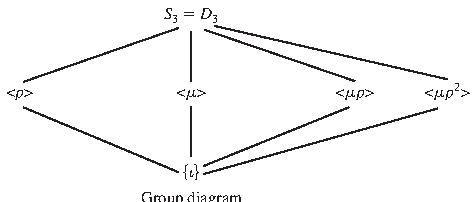
\includegraphics[width=0.651\linewidth,height=.8\textheight,keepaspectratio]{assets/p433_22.pdf}\end{center}
\end{BookFloat}

\begin{BookFloat}{answers-p433-29}
\begin{center}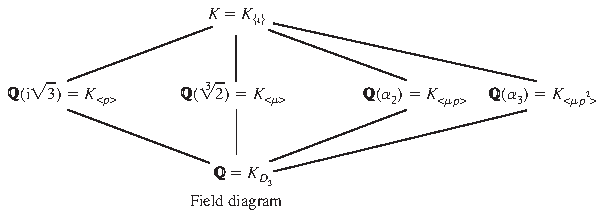
\includegraphics[width=0.824\linewidth,height=.8\textheight,keepaspectratio]{assets/p433_24.pdf}\end{center}
\end{BookFloat}

\BookExercise{13.}{The splitting field of \BookInline{(x^{3}- 1)\in \mathbb{Q}[x]} is \BookInline{\mathbb{Q} ( i \sqrt { 3 } )} and the group is cyclic of order 2 with elements\BookInline{:\iota,\allowbreak } where \BookInline{\iota } is the identity map of \BookInline{\mathbb{Q}(i\sqrt{3}),\allowbreak } and \BookInline{\sigma,\allowbreak } where \BookInline{\sigma (i\sqrt{3})= - i\sqrt{3}.}}

\BookExercise{5.}{\textbf{1. a} \BookInline{F} \textbf{c}\BookInline{.T} \textbf{e}\BookInline{.T} \textbf{g}\BookInline{.F} \textbf{i}\BookInline{.F}}

\BookExercise{25.}{\textit{Partial answer}\BookInline{:G(K/(E\vee L))= G(K/E)\cap G(K/L)}}

\end{BookBody}

% Source PDF page 434; original printed page 417
\BookSource{434}{417}
\BookNarrativefalse

\begin{BookBody}

\BookSectionTitle{47}{Illustrations of Galois Theory}

\BookExercise{5.}{The group is cyclic of order 5, and its elements are}

\begin{BookFloat}{answers-p434-3}
\begin{center}\begin{adjustbox}{max width=\linewidth}
\renewcommand{\arraystretch}{1.3}
\begin{tabular}{c|c|c|c|c|c}
 & $\iota$ & $\sigma_1$ & $\sigma_2$ & $\sigma_3$ & $\sigma_4$\\\hline
$\sqrt[5]{2}\to$ & $\sqrt[5]{2}$ & $\zeta\sqrt[5]{2}$ & $\zeta^2\sqrt[5]{2}$ & $\zeta^3\sqrt[5]{2}$ & $\zeta^4\sqrt[5]{2}$
\end{tabular}\end{adjustbox}\end{center}
\end{BookFloat}

where \BookInline{\sqrt { 2 }} is the real 5th root of 2.

\BookExercise{7.}{The splitting field of \BookInline{x^{8}- 1} over \BookInline{\mathbb{Q}} is the same as the splitting field of \BookInline{x^{4}+ 1} over \BookInline{\mathbb{Q},\allowbreak } so a complete description is contained in Example 47.7. (This is the easiest way to answer the problem.)}

\BookExercise{9.}{\textbf{. a} \BookInline{s_{1}^{2}- 2s_{2}} \textbf{b.} \BookInline{\frac { s _ { 1 } s _ { 2 } - 3 s _ { 3 } } { s _ { 3 } }}}

\BookSectionTitle{48}{Cyclotomic Extensions}

\BookExercise{3.}{\textbf{a.} 16 \textbf{b.} 400 \textbf{c.} 2160}

\BookExercise{5.}{30}

\BookExercise{7.}{\textbf{a}\BookInline{.T} \textbf{c}\BookInline{.F} \textbf{e}\BookInline{.T} \textbf{g}\BookInline{.T} \textbf{i}\BookInline{.F}}

\BookExercise{9.}{\BookInline{\Phi _{1}(x)= x- 1} \BookInline{\Phi _{2}(x)= x+ 1} \BookInline{\Phi _{3}(x)= x^{2}+ x+ 1} \BookInline{\Phi _{4}(x)= x^{2}+ 1} \BookInline{\Phi _{5}(x)= x^{4}+ x^{3}+ x^{2}+ x+ 1} \BookInline{\Phi _{6}(x)= x^{2}- x+ 1}}

\BookSectionTitle{49}{Insolvability of the Quintic}

\BookExercise{1.}{No. Yes\BookInline{,\allowbreak K} is an extension of \BookInline{\mathbb{Z}_{2}} by radicals.}

\BookExercise{3.}{\textbf{. a} \BookInline{T} \textbf{c}\BookInline{.T} \textbf{e}\BookInline{.T} \textbf{g}\BookInline{.T} \textbf{i}\BookInline{.F(x^{3}- 2x} over \BookInline{\mathbb{Q}} gives a counterexample.)}

\BookTextHeading{\textbf{APPENDIX}}

\begin{center}\begin{adjustbox}{max width=\linewidth}\BookInline{\displaystyle \begin{bmatrix} - 3 + 2i & - 1 - 4i \\ 2 & - i \\ 0 & - i \end{bmatrix}}\end{adjustbox}\end{center}

\begin{center}\begin{adjustbox}{max width=\linewidth}\BookInline{\displaystyle \begin{bmatrix} 2 & 1 \\ 2 & 7 \end{bmatrix}}\end{adjustbox}\end{center}

\BookInline{\Big[\Big]} \BookInline{\Big[\Big]}

\BookExercise{5.}{\BookInline{\begin{bmatrix} 5 & 16 & -3 \\ 0 & -18 & 24 \end{bmatrix}}}

\BookExercise{7.}{\BookInline{\begin{bmatrix} 1 & - i \\ 4 - 6i & - 2 - 2i \end{bmatrix}}}

\BookInline{\Big[\Big]} \BookInline{\Big[\Big]}

\BookExercise{9.}{\BookInline{\begin{bmatrix} 8 & - 8 i \\ 8 i & \quad 8 \end{bmatrix}}}

\BookExercise{11.}{\BookInline{\begin{bmatrix} 0 & - 1 \\ 1 & \quad 0 \end{bmatrix}}}

\BookExercise{13.}{\BookInline{- 48}}

\end{BookBody}
\ifdefined\BookMaster\let\BookFinish\relax\else\def\BookFinish{\end{document}}\fi\BookFinish

\clearpage
% !TeX program = xelatex
\ifdefined\BookMaster\else
\documentclass[11pt,oneside]{article}
% !TeX program = xelatex
\usepackage[b5paper,left=22mm,right=22mm,top=20mm,bottom=22mm,footskip=11mm]{geometry}
\usepackage{fontspec}
\setmainfont{TeX Gyre Termes}
\setsansfont{TeX Gyre Heros}
\usepackage{amsmath,amssymb,mathtools,amsthm}
\renewcommand{\cdots}{\mathinner{\cdotp\cdotp\cdotp}}
\usepackage{graphicx,adjustbox,array,booktabs,longtable,multirow,enumitem,changepage,needspace}
\usepackage[table]{xcolor}
\usepackage{fancyhdr}
\raggedbottom
\interfootnotelinepenalty=10000
\newcommand{\BookFootnote}[2]{\begingroup\renewcommand{\thefootnote}{\fnsymbol{footnote}}\footnote[#1]{#2}\endgroup}
\newcommand{\BookFootnoteMark}[1]{\begingroup\renewcommand{\thefootnote}{\fnsymbol{footnote}}\footnotemark[#1]\endgroup}
\newcommand{\BookFootnoteText}[2]{\begingroup\renewcommand{\thefootnote}{\fnsymbol{footnote}}\footnotetext[#1]{#2}\endgroup}
\newenvironment{BookFloat}[1]{\par\addvspace{.6\baselineskip}\noindent\def\BookFloatID{#1}\begin{minipage}{\linewidth}\phantomsection\label{bookfloat:#1:start}}{\phantomsection\label{bookfloat:\BookFloatID:end}\end{minipage}\par\addvspace{.6\baselineskip}}

\usepackage[unicode,hidelinks]{hyperref}
\pagestyle{fancy}
\fancyhf{}
\newcommand{\BookFooter}{}
\fancyfoot[L]{\parbox[b]{\dimexpr\textwidth-15mm}{\footnotesize\BookFooter}}
\fancyfoot[R]{\footnotesize\thepage}
\renewcommand{\headrulewidth}{0pt}
\renewcommand{\footrulewidth}{0pt}
\setlength{\parindent}{0pt}
\setlength{\parskip}{0.2em}
\setlength{\emergencystretch}{3em}
\setlist{nosep,leftmargin=1.7em,labelsep=.65em}
\newif\ifBookNarrative
\BookNarrativetrue
\newenvironment{BookBody}{\setlength{\parindent}{0pt}}{}
\newcommand{\BookStatement}[1]{\par\addvspace{.6\baselineskip}\noindent #1\enspace\ignorespaces}
\newcommand{\BookLabel}[1]{\par\addvspace{.6\baselineskip}\needspace{3\baselineskip}\noindent\textbf{#1}\quad\ignorespaces}
\newcommand{\BookHeading}[1]{\par\addvspace{\baselineskip}\needspace{4\baselineskip}\noindent{\large\bfseries #1}\par\medskip}
\newcommand{\BookSubheading}[1]{\par\addvspace{.7\baselineskip}\needspace{3\baselineskip}\noindent{\bfseries #1}\par\smallskip}
\newcommand{\BookTextHeading}[1]{\par\addvspace{.7\baselineskip}\needspace{3\baselineskip}\noindent #1\par\smallskip}
\newcommand{\BookSectionTitle}[2]{\par\addvspace{1.2\baselineskip}\needspace{5\baselineskip}\noindent\colorbox{gray!25}{\sffamily\bfseries\small SECTION #1}\quad{\large\bfseries #2}\par\medskip}
\newcommand{\BookExerciseTitle}[1]{\par\addvspace{\baselineskip}\needspace{4\baselineskip}\noindent{\color{gray}\rule{1.5mm}{1.5mm}}\enspace{\large\bfseries Exercises #1}\par\medskip}
\newcommand{\BookBullet}[1]{\begin{list}{\textbullet}{\setlength{\leftmargin}{1.7em}\setlength{\labelwidth}{1em}\setlength{\labelsep}{.7em}\setlength{\topsep}{0pt}\setlength{\parsep}{0pt}\setlength{\itemsep}{0pt}}\item #1\end{list}}
\newcommand{\BookExercise}[2]{\begin{list}{\textbf{#1}}{\setlength{\leftmargin}{2.2em}\setlength{\labelwidth}{1.5em}\setlength{\labelsep}{.7em}\setlength{\topsep}{.15em}\setlength{\parsep}{0pt}\setlength{\itemsep}{0pt}}\item #2\end{list}}
\newcommand{\BookEnd}[1]{\unskip\nobreak\hfill\ensuremath{#1}}
\newcommand{\BookSource}[2]{\phantomsection\label{sourcepage:#1}} % Source-page anchors, retained through reflow.
\usepackage{multicol}
\usepackage{tikz}
\newcommand{\BookPartEntry}[2]{\par\noindent\makebox[17mm][l]{\bfseries Section #1}#2\par}
\newcommand{\BookPartTitle}[3]{\par\bigskip\noindent\begin{tikzpicture}\node[anchor=north west,inner sep=0pt,outer sep=0pt] (bookpart) at (0,0) {\begin{minipage}{\dimexpr\linewidth-.5pt}\hspace*{26mm}\begin{minipage}[t]{\dimexpr\linewidth-26mm}\begin{adjustbox}{max width=\linewidth}{\fontsize{20}{24}\selectfont\bfseries #2}\end{adjustbox}\par\vspace{6mm}\hrule\vspace{6mm}{\sffamily\footnotesize\setlength{\parskip}{.3em}#3}\vspace{3mm}\end{minipage}\end{minipage}};\path[shade,top color=gray!60,bottom color=white] (0,0) rectangle ([xshift=24mm]bookpart.south west);\node[anchor=north,font=\sffamily\bfseries\small] at (12mm,-2mm) {PART};\node[anchor=north,font=\sffamily\bfseries\Huge] at (12mm,-7mm) {#1};\end{tikzpicture}\par\bigskip}
\newsavebox{\BookMathBox}
\makeatletter
\newcommand{\BookInline}[1]{\leavevmode\hskip0pt\relax\begingroup\in@{\begin}{#1}\ifin@\sbox{\BookMathBox}{\(#1\)}\ifdim\wd\BookMathBox>\dimexpr\linewidth-1em\relax\resizebox{\dimexpr\linewidth-1em\relax}{!}{\usebox{\BookMathBox}}\else\(#1\)\fi\else\in@{\left}{#1}\ifin@\sbox{\BookMathBox}{\(#1\)}\ifdim\wd\BookMathBox>\dimexpr\linewidth-1em\relax\resizebox{\dimexpr\linewidth-1em\relax}{!}{\usebox{\BookMathBox}}\else\(#1\)\fi\else\(#1\)\fi\fi\endgroup\hskip0pt\relax}
\makeatother
\DeclareMathOperator{\Aut}{Aut}
\DeclareMathOperator{\End}{End}
\DeclareMathOperator{\Hom}{Hom}
\DeclareMathOperator{\GF}{GF}
\DeclareMathOperator{\irr}{irr}
\DeclareMathOperator{\lt}{lt}
\DeclareMathOperator{\lp}{lp}
\providecommand{\textcircled}[1]{\textnormal{(#1)}}

\begin{document}
\fi
\renewcommand{\BookFooter}{Notations and Index}
\pdfbookmark[0]{Notations and Index}{notations_and_index}
\ifdefined\BookMaster\else\setcounter{page}{397}\fi
% Source PDF page 414; original printed page 397
\BookSource{414}{397}
\BookHeading{Notations}
\begingroup\footnotesize
\renewcommand{\arraystretch}{1.3}
\begin{longtable}{@{}>{\raggedleft\arraybackslash}p{.30\linewidth}@{\hspace{1em}}>{\raggedright\arraybackslash}p{.65\linewidth}@{}}
\BookInline{\in,\allowbreak a\in S} & membership, 1\\
\BookInline{\emptyset } & empty set, 1\\
\BookInline{\notin,\allowbreak a\notin S} & nonmembership, 1\\
\BookInline{\{x\mid P(x)\}} & set of all \BookInline{x} such that \BookInline{P(x),\allowbreak 1}\\
\BookInline{B\subseteq A} & set inclusion, 2\\
\BookInline{B\subset A} & subset \BookInline{B\neq A,\allowbreak 2}\\
\BookInline{A\times B} & Cartesian product of sets, 2\\
\BookInline{\mathbb{Z}} & integers, 2\\
\BookInline{\mathbb{Q}} & rational numbers, 2\\
\BookInline{\mathbb{R}} & real numbers, 3\\
\BookInline{\mathbb{C}} & complex numbers, 3\\
\BookInline{\mathbb{Z}^{+ },\allowbreak \mathbb{Q}^{+ },\allowbreak \mathbb{R}^{+ }} & positive elements of \BookInline{\mathbb{Z},\allowbreak \mathbb{Q},\allowbreak \mathbb{R},\allowbreak 3}\\
\BookInline{\mathbb{Z}^{\ast },\allowbreak \mathbb{Q}^{\ast },\allowbreak \mathbb{R}^{\ast },\allowbreak \mathbb{C}^{\ast }} & nonzero elements of \BookInline{\mathbb{Z},\allowbreak \mathbb{Q},\allowbreak \mathbb{R},\allowbreak \mathbb{C},\allowbreak 3}\\
\BookInline{\mathcal{R}} & relation, 3\\
\BookInline{|A|} & number of elements in \BookInline{A,\allowbreak 3;} as order of group, 41\\
\BookInline{\phi:A\to B} & mapping of \BookInline{A} into \BookInline{B} by \BookInline{\phi,\allowbreak 3}\\
\BookInline{\phi (a)} & image of element \BookInline{a} under \BookInline{\phi,\allowbreak 4}\\
\BookInline{\phi [A]} & image of set \BookInline{A} under \BookInline{\phi,\allowbreak 4}\\
\BookInline{\leftrightarrow } & one-to-one correspondence, 4\\
\BookInline{\phi^{-1}} & the inverse function of \BookInline{\phi,\allowbreak 4}\\
\BookInline{\aleph _{0}} & cardinality of \BookInline{\mathbb{Z}^{+ },\allowbreak 4}\\
\BookInline{\overline{x}} & cell containing \BookInline{x\in S} in a partition of \BookInline{S,\allowbreak 6}\\
\BookInline{\mathbb{Z}/n\mathbb{Z}} & residue classes modulo \BookInline{n_{\iota },\allowbreak 6}\\
\BookInline{\equiv _{n},\allowbreak a\equiv b(}mod \BookInline{n)} & congruence modulo \BookInline{n,\allowbreak 6}\\
\BookInline{\mathcal{P}(A)} & power set of \BookInline{A,\allowbreak 8}\\
\BookInline{U} & set of all \BookInline{z\in \mathbb{C}} such that \BookInline{|z|= 1,\allowbreak 36}\\
\BookInline{\mathbb{R}_{c}} & set of all \BookInline{x\in \mathbb{R}} such that \BookInline{0\leq x<c,\allowbreak 33}\\
\BookInline{+ _{c}} & addition modulo \BookInline{c,\allowbreak 33}\\
\BookInline{U_{n}} & group of \BookInline{n}th roots of unity, 37\\
\end{longtable}
\endgroup

% Source PDF page 415; original printed page 398
\BookSource{415}{398}
\begingroup\footnotesize
\renewcommand{\arraystretch}{1.3}
\begin{longtable}{@{}>{\raggedleft\arraybackslash}p{.30\linewidth}@{\hspace{1em}}>{\raggedright\arraybackslash}p{.65\linewidth}@{}}
\BookInline{\mathbb{Z}_{n}} & \BookInline{\{0,\allowbreak 1,\allowbreak 2,\allowbreak \cdots,\allowbreak n- 1\},\allowbreak 32} cyclic group \BookInline{\{0,\allowbreak 1,\allowbreak \cdots,\allowbreak n- 1\}} under addition modulo \BookInline{n,\allowbreak 38} ring \BookInline{\{0,\allowbreak 1,\allowbreak \cdots,\allowbreak n- 1\}} under addition and multiplication modulo \BookInline{n,\allowbreak 189}\\
\BookInline{\ast,\allowbreak a\ast b} & binary operation, 11\\
\BookInline{\circ,\allowbreak f\circ g,\allowbreak \sigma \tau } & function composition, 14, 41\\
\BookInline{e} & identity element, 20\\
\BookInline{M_{m\times n}(S)} & \BookInline{m\times n} matrices with entries from \BookInline{S,\allowbreak 22,\allowbreak 393}\\
\BookInline{M_{n}(S)} & \BookInline{n\times n} matrices with entries from \BookInline{S,\allowbreak 22,\allowbreak 393}\\
\textit{GL}\BookInline{(n,\allowbreak \mathbb{R})} & general linear group of degree \BookInline{n,\allowbreak 22,\allowbreak 23}\\
det\BookInline{(A)} & determinant of square matrix \BookInline{A,\allowbreak 28,\allowbreak 395}\\
\BookInline{a^{- 1},\allowbreak - a} & inverse of \BookInline{a,\allowbreak 15}\\
\BookInline{H\leq G;K\leq L} & subgroup inclusion, 52; substructure inclusion, 192\\
\BookInline{H<G;K<L} & subgroup \BookInline{H\neq G,\allowbreak 52;} substructure \BookInline{K\neq L,\allowbreak 192}\\
\BookInline{\langle a\rangle } & cyclic subgroup generated by \BookInline{a,\allowbreak 56} principal ideal generated by \BookInline{a,\allowbreak 256}\\
\BookInline{n\mathbb{Z}} & subgroup of \BookInline{\mathbb{Z}} generated by \BookInline{n,\allowbreak 56} subring (ideal) of \BookInline{\mathbb{Z}} generated by \BookInline{n,\allowbreak 245}\\
\BookInline{A^{T}} & transpose of \BookInline{A,\allowbreak 57}\\
gcd & greatest common divisor, 63, 283, 304\\
\BookInline{\begin{gathered}[t]\displaystyle\bigcap_{i\in I} S_i,\\S_1\cap S_2\cap\cdots\cap S_n\end{gathered}} & intersection of sets, 71\\
\BookInline{S_{A}} & group of permutations of \BookInline{A,\allowbreak 43}\\
\BookInline{\iota } & identity map, 43\\
\BookInline{S_{n}} & symmetric group on \BookInline{n} letters, 43\\
\BookInline{n!} & \BookInline{n} factorial, 43\\
\BookInline{D_{n}} & \BookInline{n}th dihedral group, 47\\
\BookInline{A_{n}} & alternating group on \BookInline{n} letters, 84\\
\BookInline{aH,\allowbreak a+ H} & left coset of \BookInline{H} containing \BookInline{a,\allowbreak 98}\\
\BookInline{Ha,\allowbreak H+ a} & right coset of \BookInline{H} containing \BookInline{a,\allowbreak 100}\\
\BookInline{(G:H)} & index of \BookInline{H} in \BookInline{G,\allowbreak 137}\\
\BookInline{\varphi } & Euler phi-function, 105, 204\\
\BookInline{\begin{gathered}[t]\displaystyle\prod_{i=1}^{n} B_i,\\B_1\times B_2\times\cdots\times B_n\end{gathered}} & Cartesian product of sets, 88\\
\BookInline{\displaystyle\prod_{i=1}^{n} G_i} & direct product of groups, 88, 89\\
\BookInline{\displaystyle\bigoplus_{i=1}^{n} G_i} & direct sum of groups, 89\\
lcm & least common multiple, 90\\
\BookInline{\overline{G_i}} & natural subgroup of \BookInline{\prod _{i= 1}^{n}G_{i},\allowbreak 91}\\
\BookInline{H\lhd G} & \BookInline{H} normal subgroup of \BookInline{G,\allowbreak 116}\\
SL \BookInline{(n,\allowbreak \mathbb{R})} & special linear group, 117\\
\BookInline{\phi _{a}} & evaluation homomorphism, 191\\
\BookInline{\pi _{i}} & projection onto \BookInline{i}th component, 248\\
\BookInline{\phi ^{- 1}[B]} & inverse image of the set \BookInline{B} under \BookInline{\phi,\allowbreak 78}\\
Ker\BookInline{(\phi )} & kernel of homomorphism \BookInline{\phi,\allowbreak 78}\\
\BookInline{G/N;R/N} & factor group, 117; factor ring, 247\\
\BookInline{\gamma } & canonical residue class map, 118, 119\\
\BookInline{i_{g}} & inner automorphism, 120\\
\BookInline{Z(G)} & center of the group \BookInline{G,\allowbreak 130}\\
\BookInline{C} & commutator subgroup, 130\\
\BookInline{X_{g}} & subset of elements of \BookInline{X} fixed by \BookInline{g,\allowbreak 136}\\
\BookInline{G_{x}} & isotropy subgroup of elements of \BookInline{G} leaving \BookInline{x} fixed, 137\\
\BookInline{Gx} & orbit of \BookInline{x} under \BookInline{G,\allowbreak 143}\\
\BookInline{R[x]} & polynomial ring with coefficients in \BookInline{R,\allowbreak 220}\\
\BookInline{R[x_{1},\allowbreak x_{2},\allowbreak \cdots,\allowbreak x_{n}]} & polynomials in \BookInline{n} indeterminates, 299\\
\BookInline{F(x)} & field of quotients of \BookInline{F[x],\allowbreak 222}\\
F\BookInline{(x_{1},\allowbreak \cdots,\allowbreak x_{n})} & field of rational functions in \BookInline{n} indeterminates, 223\\
\end{longtable}
\endgroup

% Source PDF page 416; original printed page 399
\BookSource{416}{399}
\begingroup\footnotesize
\renewcommand{\arraystretch}{1.3}
\begin{longtable}{@{}>{\raggedleft\arraybackslash}p{.30\linewidth}@{\hspace{1em}}>{\raggedright\arraybackslash}p{.65\linewidth}@{}}
\BookInline{\Phi _{p}(x)} & cyclotomic polynomial of degree \BookInline{p- 1,\allowbreak 236}\\
End\BookInline{(A)} & endomorphisms of \BookInline{A,\allowbreak 260}\\
\BookInline{RG} & group ring, 262\\
\BookInline{FG} & group algebra over the field \BookInline{F,\allowbreak 263}\\
\BookInline{\mathbb{H}} & quaternions, 264, 265\\
ACC & ascending chain condition, 280\\
\BookInline{F^{n}} & Cartesian product, 299\\
\BookInline{F[}\textbf{x}] & ring of polynomials in \BookInline{x_{1},\allowbreak \cdots,\allowbreak x_{n}} over \BookInline{F,\allowbreak 299}\\
\BookInline{V(S)} & algebraic variety of polynomials in \BookInline{S,\allowbreak 300}\\
\BookInline{\langle b_{1},\allowbreak \cdots,\allowbreak b_{r}\rangle } & ideal generated by elements \BookInline{b_{1},\allowbreak \cdots,\allowbreak b_{r},\allowbreak 300}\\
lt\BookInline{(f)} & leading term of the polynomial \BookInline{f,\allowbreak 306}\\
lp\BookInline{(f)} & power product of lt\BookInline{(f),\allowbreak 306}\\
irr\BookInline{(\alpha,\allowbreak F)} & irreducible polynomial for \BookInline{\alpha } over \BookInline{F,\allowbreak 317}\\
deg\BookInline{(\alpha,\allowbreak F)} & degree of \BookInline{\alpha } over \BookInline{F,\allowbreak 317}\\
\BookInline{F(\alpha )} & field obtained by adjoining \BookInline{\alpha } to field \BookInline{F,\allowbreak 317}\\
\BookInline{[E:F]} & degree of \BookInline{E} over \BookInline{F,\allowbreak 321}\\
\BookInline{F(\alpha _{1},\allowbreak \cdots,\allowbreak \alpha _{n})} & field obtained by adjoining \BookInline{\alpha _{1},\allowbreak \cdots,\allowbreak \alpha _{n}} to \BookInline{F,\allowbreak 323}\\
\BookInline{F_{E}} & algebraic closure of \BookInline{F} in \BookInline{E,\allowbreak 325}\\
\BookInline{\overline{F}} & an algebraic closure of \BookInline{F,\allowbreak 325,\allowbreak 326}\\
GF\BookInline{(p^{n})} & Galois field of order \BookInline{p^{n},\allowbreak 337}\\
\BookInline{HN} & product set, 148\\
\BookInline{H\vee N} & subgroup join, 148\\
\BookInline{N[H]} & normalizer of \BookInline{H,\allowbreak 152}\\
\BookInline{F[A]} & free group on \BookInline{A,\allowbreak 175}\\
\BookInline{(x_{j}:r_{i})} & group presentation, 181\\
\BookInline{a\mid b} & \BookInline{a} divides (is a factor of\BookInline{)\; b,\allowbreak 278}\\
UFD & unique factorization domain, 278\\
PID & principal ideal domain, 278\\
\BookInline{\begin{gathered}[t]\displaystyle\bigcup_{i\in I} S_i,\\S_1\cup S_2\cup\cdots\cup S_n\end{gathered}} & union of sets, 280\\
\BookInline{\nu} & Euclidean norm, 288\\
\BookInline{N(\alpha )} & norm of \BookInline{\alpha,\allowbreak 294,\allowbreak 296}\\
\BookInline{\psi_{\alpha,\beta}} & conjugation isomorphism of \BookInline{F(\alpha )} with \BookInline{F(\beta ),\allowbreak 347}\\
\BookInline{E_{\{\sigma_i\}},\ E_H} & subfield of \BookInline{E} fixed by all \BookInline{\sigma _{i}} or all \BookInline{\sigma \in H,\allowbreak 345}\\
\BookInline{G(E/F)} & automorphism group of \BookInline{E} over \BookInline{F,\allowbreak 346}\\
\BookInline{\lambda (E)} & automorphisms that fix \BookInline{E,\allowbreak 367}\\
\end{longtable}
\endgroup

% Source PDF page 436; original printed page 419
\BookSource{436}{419}
\BookHeading{Index}
\begin{multicols}{2}\footnotesize\setlength{\parskip}{.15em}
\begingroup\hangindent=0.00em\hangafter=0\noindent Abel, Niels Henrik, 21, 150, 191, 385\par\endgroup
\begingroup\hangindent=0.00em\hangafter=0\noindent Abelian extension, 370\par\endgroup
\begingroup\hangindent=0.00em\hangafter=0\noindent Abelian group(s), 20\par\endgroup
\begingroup\hangindent=1.00em\hangafter=0\noindent finitely-generated, fundamental theorems of, 92, 93\par\endgroup
\begingroup\hangindent=1.00em\hangafter=0\noindent free, 167\par\endgroup
\begingroup\hangindent=1.00em\hangafter=0\noindent torsion free, 96, 119\par\endgroup
\begingroup\hangindent=0.00em\hangafter=0\noindent Absolute value, 34\par\endgroup
\begingroup\hangindent=0.00em\hangafter=0\noindent Action\par\endgroup
\begingroup\hangindent=1.00em\hangafter=0\noindent faithful, 133\par\endgroup
\begingroup\hangindent=1.00em\hangafter=0\noindent on a group, 132\par\endgroup
\begingroup\hangindent=1.00em\hangafter=0\noindent transitive, 133\par\endgroup
\begingroup\hangindent=0.00em\hangafter=0\noindent Addition\par\endgroup
\begingroup\hangindent=1.00em\hangafter=0\noindent modulo \BookInline{2\pi,\allowbreak 37}\par\endgroup
\begingroup\hangindent=1.00em\hangafter=0\noindent modulo \BookInline{c,\allowbreak 33}\par\endgroup
\begingroup\hangindent=1.00em\hangafter=0\noindent modulo \BookInline{n,\allowbreak 32,\allowbreak 65}\par\endgroup
\begingroup\hangindent=0.00em\hangafter=0\noindent Additive identity, 14\par\endgroup
\begingroup\hangindent=0.00em\hangafter=0\noindent Adjoining elements to field, 321\par\endgroup
\begingroup\hangindent=0.00em\hangafter=0\noindent Al-Tusi Sharaf al-Din, 224\par\endgroup
\begingroup\hangindent=0.00em\hangafter=0\noindent Algebra\par\endgroup
\begingroup\hangindent=1.00em\hangafter=0\noindent fundamental theorem of, 257, 324\par\endgroup
\begingroup\hangindent=1.00em\hangafter=0\noindent group, 261\par\endgroup
\begingroup\hangindent=0.00em\hangafter=0\noindent Algebraic closure, 324\par\endgroup
\begingroup\hangindent=0.00em\hangafter=0\noindent Algebraic closure of \BookInline{F} in \BookInline{E,\allowbreak 323}\par\endgroup
\begingroup\hangindent=0.00em\hangafter=0\noindent Algebraic element over \BookInline{F,\allowbreak 313}\par\endgroup
\begingroup\hangindent=0.00em\hangafter=0\noindent Algebraic extension, 319\par\endgroup
\begingroup\hangindent=0.00em\hangafter=0\noindent Algebraic integer, 378\par\endgroup
\begingroup\hangindent=0.00em\hangafter=0\noindent Algebraic number, 314\par\endgroup
\begingroup\hangindent=0.00em\hangafter=0\noindent Algebraic number theory, 294\par\endgroup
\begingroup\hangindent=0.00em\hangafter=0\noindent Algebraic variety, 298\par\endgroup
\begingroup\hangindent=0.00em\hangafter=0\noindent Algebraically closed field, 323, 327\par\endgroup
\begingroup\hangindent=0.00em\hangafter=0\noindent Alphabet, 172\par\endgroup
\begingroup\hangindent=0.00em\hangafter=0\noindent Alternating group on \BookInline{n} letters, 84\par\endgroup
\begingroup\hangindent=0.00em\hangafter=0\noindent Antisymmetric law, 324\par\endgroup
\begingroup\hangindent=0.00em\hangafter=0\noindent Arc\par\endgroup
\begingroup\hangindent=1.00em\hangafter=0\noindent of a diagraph, 72\par\endgroup
\begingroup\hangindent=1.00em\hangafter=0\noindent of a graph, 308\par\endgroup
\begingroup\hangindent=0.00em\hangafter=0\noindent Arithmetic, fundamental theorem of, 280\par\endgroup
\begingroup\hangindent=0.00em\hangafter=0\noindent Artin, Emil, 225\par\endgroup
\begingroup\hangindent=0.00em\hangafter=0\noindent Ascending central series, 163\par\endgroup
\begingroup\hangindent=0.00em\hangafter=0\noindent Ascending chain condition, 278, 286\par\endgroup
\begingroup\hangindent=0.00em\hangafter=0\noindent Aschbacher, Michael, 127\par\endgroup
\begingroup\hangindent=0.00em\hangafter=0\noindent Associates, 276\par\endgroup
\begingroup\hangindent=0.00em\hangafter=0\noindent Associative operation, 13, 20\par\endgroup
\begingroup\hangindent=0.00em\hangafter=0\noindent Automorphism, 341\par\endgroup
\begingroup\hangindent=1.00em\hangafter=0\noindent of a field, 345\par\endgroup
\begingroup\hangindent=1.00em\hangafter=0\noindent Frobenius, 349\par\endgroup
\begingroup\hangindent=1.00em\hangafter=0\noindent of a group, 68, 118\par\endgroup
\begingroup\hangindent=1.00em\hangafter=0\noindent group of, 345\par\endgroup
\begingroup\hangindent=1.00em\hangafter=0\noindent inner, 118\par\endgroup
\begingroup\hangindent=0.00em\hangafter=0\noindent Axiom of choice, 324, 325\par\endgroup
\begingroup\hangindent=0.00em\hangafter=0\noindent Axis of reflection, 105\par\endgroup
\begingroup\hangindent=0.00em\hangafter=0\noindent Banach, Stefan, 268\par\endgroup
\begingroup\hangindent=0.00em\hangafter=0\noindent Basis\par\endgroup
\begingroup\hangindent=1.00em\hangafter=0\noindent for a finitely-generated abelian group, 176\par\endgroup
\begingroup\hangindent=1.00em\hangafter=0\noindent for a free abelian group, 167\par\endgroup
\begingroup\hangindent=1.00em\hangafter=0\noindent Gröbner, 305\par\endgroup
\begingroup\hangindent=1.00em\hangafter=0\noindent for an ideal, 298\par\endgroup
\begingroup\hangindent=1.00em\hangafter=0\noindent for a vector space, 270\par\endgroup
\begingroup\hangindent=0.00em\hangafter=0\noindent Bessy, Bernard Frenicle de, 201\par\endgroup
\begingroup\hangindent=0.00em\hangafter=0\noindent Betti number, 92\par\endgroup
\begingroup\hangindent=0.00em\hangafter=0\noindent Bijection, 4\par\endgroup
\begingroup\hangindent=0.00em\hangafter=0\noindent Binary operation, 11\par\endgroup
\begingroup\hangindent=0.00em\hangafter=0\noindent Bit, 237\par\endgroup
\begingroup\hangindent=0.00em\hangafter=0\noindent Bit errors, 239\par\endgroup
\begingroup\hangindent=0.00em\hangafter=0\noindent Blip group, 177\par\endgroup
\begingroup\hangindent=0.00em\hangafter=0\noindent Bloom, David M., 82\par\endgroup
\begingroup\hangindent=0.00em\hangafter=0\noindent Blop group, 177\par\endgroup
\begingroup\hangindent=0.00em\hangafter=0\noindent Boolean ring, 194\par\endgroup
\begingroup\hangindent=0.00em\hangafter=0\noindent Bourbaki, Nicholas, 4, 177, 326\par\endgroup
\begingroup\hangindent=0.00em\hangafter=0\noindent Brahmagupta, 288\par\endgroup
\begingroup\hangindent=0.00em\hangafter=0\noindent Burnside, William, 127, 152\par\endgroup
\begingroup\hangindent=0.00em\hangafter=0\noindent Burnside’s formula, 141\par\endgroup
\begingroup\hangindent=0.00em\hangafter=0\noindent Cancellation laws, 23, 196\par\endgroup
\begingroup\hangindent=0.00em\hangafter=0\noindent Cardano, Girolamo, 224, 385\par\endgroup
\begingroup\hangindent=0.00em\hangafter=0\noindent Cardinality, 3, 4\par\endgroup
\begingroup\hangindent=0.00em\hangafter=0\noindent Cartesian product, 2, 88\par\endgroup
\begingroup\hangindent=0.00em\hangafter=0\noindent Cauchy Augustin-Louis, 42\par\endgroup
\begingroup\hangindent=0.00em\hangafter=0\noindent Cauchy’s theorem, 136\par\endgroup
\begingroup\hangindent=0.00em\hangafter=0\noindent Cayley, Arthur, 72, 81, 178\par\endgroup
\begingroup\hangindent=0.00em\hangafter=0\noindent Cayley digraph, 72\par\endgroup
\begingroup\hangindent=0.00em\hangafter=0\noindent Cayley’s theorem, 79\par\endgroup
\begingroup\hangindent=0.00em\hangafter=0\noindent Cell, 5\par\endgroup
\begingroup\hangindent=0.00em\hangafter=0\noindent Center of a group, 60, 128, 163\par\endgroup
\begingroup\hangindent=0.00em\hangafter=0\noindent Chain(s), 324\par\endgroup
\begingroup\hangindent=0.00em\hangafter=0\noindent Chain condition,\par\endgroup
\begingroup\hangindent=1.00em\hangafter=0\noindent ascending, 278, 286\par\endgroup
\begingroup\hangindent=1.00em\hangafter=0\noindent descending, 286\par\endgroup
\begingroup\hangindent=0.00em\hangafter=0\noindent Characteristic of a ring, 198\par\endgroup
\begingroup\hangindent=0.00em\hangafter=0\noindent Chief series, 161\par\endgroup
\begingroup\hangindent=0.00em\hangafter=0\noindent Class\par\endgroup
\begingroup\hangindent=1.00em\hangafter=0\noindent equivalence, 7\par\endgroup
\begingroup\hangindent=1.00em\hangafter=0\noindent residue modulo \BookInline{n,\allowbreak 6}\par\endgroup
\begingroup\hangindent=0.00em\hangafter=0\noindent Class equation, 156\par\endgroup
\begingroup\hangindent=0.00em\hangafter=0\noindent Closed interval, 8\par\endgroup
\begingroup\hangindent=0.00em\hangafter=0\noindent Closed set under an operation, 12, 37\par\endgroup
\begingroup\hangindent=0.00em\hangafter=0\noindent Closure, algebraic, 323\par\endgroup
\begingroup\hangindent=0.00em\hangafter=0\noindent Code, 238\par\endgroup
\begingroup\hangindent=1.00em\hangafter=0\noindent polynomial, 241\par\endgroup
\begingroup\hangindent=0.00em\hangafter=0\noindent Code word, 238\par\endgroup
\begingroup\hangindent=0.00em\hangafter=0\noindent Codomain, 3\par\endgroup
\begingroup\hangindent=0.00em\hangafter=0\noindent Coefficients\par\endgroup
\begingroup\hangindent=1.00em\hangafter=0\noindent of a polynomial, 219\par\endgroup
\begingroup\hangindent=1.00em\hangafter=0\noindent torsion, 93, 96\par\endgroup
\begingroup\hangindent=0.00em\hangafter=0\noindent Coloring of graph, 308\par\endgroup
\begingroup\hangindent=0.00em\hangafter=0\noindent Commensurable numbers, 223\par\endgroup
\begingroup\hangindent=0.00em\hangafter=0\noindent Commutative operation, 13\par\endgroup
\begingroup\hangindent=0.00em\hangafter=0\noindent Commutative ring, 189\par\endgroup
\begingroup\hangindent=0.00em\hangafter=0\noindent Commutator, 120, 128\par\endgroup
\begingroup\hangindent=0.00em\hangafter=0\noindent Commutator subgroup, 120, 128\par\endgroup
\begingroup\hangindent=0.00em\hangafter=0\noindent Comparable elements, 324\par\endgroup
\begingroup\hangindent=0.00em\hangafter=0\noindent Complex number, 3, 33\par\endgroup
\begingroup\hangindent=1.00em\hangafter=0\noindent absolute value of, 34\par\endgroup
\begingroup\hangindent=1.00em\hangafter=0\noindent multiplication of, 34\par\endgroup
\begingroup\hangindent=0.00em\hangafter=0\noindent Composition, function, 12, 14\par\endgroup
\begingroup\hangindent=1.00em\hangafter=0\noindent associativity of, 14\par\endgroup
\begingroup\hangindent=0.00em\hangafter=0\noindent Composition series, 161\par\endgroup
\begingroup\hangindent=0.00em\hangafter=0\noindent Congruence modulo \BookInline{n,\allowbreak 6}\par\endgroup
\begingroup\hangindent=0.00em\hangafter=0\noindent Conjugate elements over \BookInline{F,\allowbreak 345}\par\endgroup
\begingroup\hangindent=0.00em\hangafter=0\noindent Conjugate subgroups, 119, 120\par\endgroup
\begingroup\hangindent=0.00em\hangafter=0\noindent Conjugation, 118\par\endgroup
\begingroup\hangindent=0.00em\hangafter=0\noindent Conjugation isomorphism, 345\par\endgroup

% Source PDF page 437; original printed page 420
\BookSource{437}{420}
\begingroup\hangindent=0.00em\hangafter=0\noindent Consequence, 179\par\endgroup
\begingroup\hangindent=0.00em\hangafter=0\noindent Constant polynomial, 219\par\endgroup
\begingroup\hangindent=0.00em\hangafter=0\noindent Constructible number, 329\par\endgroup
\begingroup\hangindent=0.00em\hangafter=0\noindent Constructible polygon, 380\par\endgroup
\begingroup\hangindent=0.00em\hangafter=0\noindent Content of a polynomial, 237, 281\par\endgroup
\begingroup\hangindent=0.00em\hangafter=0\noindent Contraction, elementary, 173\par\endgroup
\begingroup\hangindent=0.00em\hangafter=0\noindent Correction of bit errors, 239\par\endgroup
\begingroup\hangindent=0.00em\hangafter=0\noindent Correspondence, one-to-one, 4\par\endgroup
\begingroup\hangindent=0.00em\hangafter=0\noindent Coset, 97\par\endgroup
\begingroup\hangindent=1.00em\hangafter=0\noindent double, 104\par\endgroup
\begingroup\hangindent=1.00em\hangafter=0\noindent left, 98\par\endgroup
\begingroup\hangindent=1.00em\hangafter=0\noindent right, 100\par\endgroup
\begingroup\hangindent=0.00em\hangafter=0\noindent Coset group, 97\par\endgroup
\begingroup\hangindent=0.00em\hangafter=0\noindent Crelle, August, 21\par\endgroup
\begingroup\hangindent=0.00em\hangafter=0\noindent Cycle(s), 44\par\endgroup
\begingroup\hangindent=1.00em\hangafter=0\noindent disjoint, 44, 45\par\endgroup
\begingroup\hangindent=1.00em\hangafter=0\noindent \BookInline{k-,\allowbreak 44}\par\endgroup
\begingroup\hangindent=0.00em\hangafter=0\noindent Cyclic extension, 371\par\endgroup
\begingroup\hangindent=0.00em\hangafter=0\noindent Cyclic group, 56, 61\par\endgroup
\begingroup\hangindent=1.00em\hangafter=0\noindent elementary properties of, 61\par\endgroup
\begingroup\hangindent=1.00em\hangafter=0\noindent finite, subgroups of, 66\par\endgroup
\begingroup\hangindent=1.00em\hangafter=0\noindent structure of, 64\par\endgroup
\begingroup\hangindent=0.00em\hangafter=0\noindent Cyclic linear code, 238\par\endgroup
\begingroup\hangindent=0.00em\hangafter=0\noindent Cyclic subgroup, 55, 61\par\endgroup
\begingroup\hangindent=0.00em\hangafter=0\noindent Cyclotomic extension, 378\par\endgroup
\begingroup\hangindent=0.00em\hangafter=0\noindent Cyclotomic polynomial, 234, 378\par\endgroup
\begingroup\hangindent=0.00em\hangafter=0\noindent Decomposable group, 93\par\endgroup
\begingroup\hangindent=0.00em\hangafter=0\noindent Decryption, 205\par\endgroup
\begingroup\hangindent=0.00em\hangafter=0\noindent Dedekind, Richard, 191, 244\par\endgroup
\begingroup\hangindent=0.00em\hangafter=0\noindent Definitions, 1\par\endgroup
\begingroup\hangindent=0.00em\hangafter=0\noindent Degree\par\endgroup
\begingroup\hangindent=1.00em\hangafter=0\noindent of \BookInline{\alpha } over \BookInline{F,\allowbreak 315}\par\endgroup
\begingroup\hangindent=1.00em\hangafter=0\noindent of an extension, 319\par\endgroup
\begingroup\hangindent=1.00em\hangafter=0\noindent of a polynomial, 219\par\endgroup
\begingroup\hangindent=0.00em\hangafter=0\noindent Derivative, 340\par\endgroup
\begingroup\hangindent=0.00em\hangafter=0\noindent Descartes, Rene, 218\par\endgroup
\begingroup\hangindent=0.00em\hangafter=0\noindent Descending chain condition, 286\par\endgroup
\begingroup\hangindent=0.00em\hangafter=0\noindent Detection of bit error, 239\par\endgroup
\begingroup\hangindent=0.00em\hangafter=0\noindent Determinant of a square matrix, 28\par\endgroup
\begingroup\hangindent=0.00em\hangafter=0\noindent Diagonal matrix, 28\par\endgroup
\begingroup\hangindent=0.00em\hangafter=0\noindent Diagram, subgroup, 53\par\endgroup
\begingroup\hangindent=0.00em\hangafter=0\noindent Digraph, 72\par\endgroup
\begingroup\hangindent=1.00em\hangafter=0\noindent arc of, 72\par\endgroup
\begingroup\hangindent=1.00em\hangafter=0\noindent vertex of, 72\par\endgroup
\begingroup\hangindent=0.00em\hangafter=0\noindent Dihedral group, 46\par\endgroup
\begingroup\hangindent=0.00em\hangafter=0\noindent Dimension of a vector space over \BookInline{F,\allowbreak } 272\par\endgroup
\begingroup\hangindent=0.00em\hangafter=0\noindent Direct product, 89\par\endgroup
\begingroup\hangindent=1.00em\hangafter=0\noindent external, 91\par\endgroup
\begingroup\hangindent=1.00em\hangafter=0\noindent internal, 91\par\endgroup
\begingroup\hangindent=1.00em\hangafter=0\noindent of rings, 187\par\endgroup
\begingroup\hangindent=0.00em\hangafter=0\noindent Direct sum, 89\par\endgroup
\begingroup\hangindent=1.00em\hangafter=0\noindent of vector spaces, 274\par\endgroup
\begingroup\hangindent=0.00em\hangafter=0\noindent Dirichlet, Peter Lejeune, 191\par\endgroup
\begingroup\hangindent=0.00em\hangafter=0\noindent Discrete frieze group, 107\par\endgroup
\begingroup\hangindent=0.00em\hangafter=0\noindent Discriminant of a polynomial, 378\par\endgroup
\begingroup\hangindent=0.00em\hangafter=0\noindent Disjoint cycles, 44, 45\par\endgroup
\begingroup\hangindent=0.00em\hangafter=0\noindent Disjoint sets, 5\par\endgroup
\begingroup\hangindent=0.00em\hangafter=0\noindent Disjoint union of \BookInline{G-}sets, 140\par\endgroup
\begingroup\hangindent=0.00em\hangafter=0\noindent Distance between two strings, 238\par\endgroup
\begingroup\hangindent=0.00em\hangafter=0\noindent Distributive law, 185\par\endgroup
\begingroup\hangindent=0.00em\hangafter=0\noindent Division algorithm\par\endgroup
\begingroup\hangindent=1.00em\hangafter=0\noindent for \BookInline{\mathbb{Z},\allowbreak 62}\par\endgroup
\begingroup\hangindent=1.00em\hangafter=0\noindent for \BookInline{F[x],\allowbreak 228,\allowbreak 286,\allowbreak 300}\par\endgroup
\begingroup\hangindent=0.00em\hangafter=0\noindent Division ring, 190\par\endgroup
\begingroup\hangindent=0.00em\hangafter=0\noindent Divisor, 276, 300\par\endgroup
\begingroup\hangindent=1.00em\hangafter=0\noindent greatest common, 63, 281\par\endgroup
\begingroup\hangindent=1.00em\hangafter=0\noindent of a polynomial, 234\par\endgroup
\begingroup\hangindent=1.00em\hangafter=0\noindent of zero, 194\par\endgroup
\begingroup\hangindent=0.00em\hangafter=0\noindent Domain\par\endgroup
\begingroup\hangindent=1.00em\hangafter=0\noindent Euclidean, 286\par\endgroup
\begingroup\hangindent=1.00em\hangafter=0\noindent of a function, 3\par\endgroup
\begingroup\hangindent=1.00em\hangafter=0\noindent integral, 196\par\endgroup
\begingroup\hangindent=1.00em\hangafter=0\noindent principal ideal, 276\par\endgroup
\begingroup\hangindent=1.00em\hangafter=0\noindent unique factorization, 276\par\endgroup
\begingroup\hangindent=0.00em\hangafter=0\noindent Double coset, 104\par\endgroup
\begingroup\hangindent=0.00em\hangafter=0\noindent Doubling the cube, 332\par\endgroup
\begingroup\hangindent=0.00em\hangafter=0\noindent Edges of graph, 308\par\endgroup
\begingroup\hangindent=0.00em\hangafter=0\noindent Eisenstein criterion, 233\par\endgroup
\begingroup\hangindent=0.00em\hangafter=0\noindent Element(s), 1\par\endgroup
\begingroup\hangindent=1.00em\hangafter=0\noindent adjoining to field, 321\par\endgroup
\begingroup\hangindent=1.00em\hangafter=0\noindent algebraic over \BookInline{F,\allowbreak 313}\par\endgroup
\begingroup\hangindent=1.00em\hangafter=0\noindent comparable, 324\par\endgroup
\begingroup\hangindent=1.00em\hangafter=0\noindent conjugate over \BookInline{F,\allowbreak 345}\par\endgroup
\begingroup\hangindent=1.00em\hangafter=0\noindent equivalent, 212\par\endgroup
\begingroup\hangindent=1.00em\hangafter=0\noindent fixed, 342\par\endgroup
\begingroup\hangindent=1.00em\hangafter=0\noindent idempotent, 19, 31, 193, 199\par\endgroup
\begingroup\hangindent=1.00em\hangafter=0\noindent identity, 14, 20\par\endgroup
\begingroup\hangindent=1.00em\hangafter=0\noindent inverse of, 20\par\endgroup
\begingroup\hangindent=1.00em\hangafter=0\noindent irreducible, 276\par\endgroup
\begingroup\hangindent=1.00em\hangafter=0\noindent maximal, 325\par\endgroup
\begingroup\hangindent=1.00em\hangafter=0\noindent nilpotent, 193, 250\par\endgroup
\begingroup\hangindent=1.00em\hangafter=0\noindent orbit of, 82, 135\par\endgroup
\begingroup\hangindent=1.00em\hangafter=0\noindent order of, 61\par\endgroup
\begingroup\hangindent=1.00em\hangafter=0\noindent prime, 280\par\endgroup
\begingroup\hangindent=1.00em\hangafter=0\noindent primitive, 360\par\endgroup
\begingroup\hangindent=1.00em\hangafter=0\noindent separable over \BookInline{F,\allowbreak 359}\par\endgroup
\begingroup\hangindent=1.00em\hangafter=0\noindent transcendental over \BookInline{F,\allowbreak 313}\par\endgroup
\begingroup\hangindent=0.00em\hangafter=0\noindent Elementary contraction, 173\par\endgroup
\begingroup\hangindent=0.00em\hangafter=0\noindent Elementary symmetric function, 372\par\endgroup
\begingroup\hangindent=0.00em\hangafter=0\noindent Empty set, 1\par\endgroup
\begingroup\hangindent=0.00em\hangafter=0\noindent Empty word, 172\par\endgroup
\begingroup\hangindent=0.00em\hangafter=0\noindent Encryption, 205\par\endgroup
\begingroup\hangindent=1.00em\hangafter=0\noindent RSA, 206\par\endgroup
\begingroup\hangindent=0.00em\hangafter=0\noindent Endomorphism, 258\par\endgroup
\begingroup\hangindent=0.00em\hangafter=0\noindent Equation, class, 156\par\endgroup
\begingroup\hangindent=0.00em\hangafter=0\noindent Equivalence class, 7\par\endgroup
\begingroup\hangindent=0.00em\hangafter=0\noindent Equivalence relation, 6\par\endgroup
\begingroup\hangindent=0.00em\hangafter=0\noindent Equivalent elements, 212\par\endgroup
\begingroup\hangindent=0.00em\hangafter=0\noindent Errors, bit, 239\par\endgroup
\begingroup\hangindent=0.00em\hangafter=0\noindent Escher M. C., 109\par\endgroup
\begingroup\hangindent=0.00em\hangafter=0\noindent Euclid, 201, 288\par\endgroup
\begingroup\hangindent=0.00em\hangafter=0\noindent Euclidean algorithm, 288\par\endgroup
\begingroup\hangindent=0.00em\hangafter=0\noindent Euclidean domain, 286\par\endgroup
\begingroup\hangindent=0.00em\hangafter=0\noindent Euclidean norm, 286\par\endgroup
\begingroup\hangindent=0.00em\hangafter=0\noindent Euler, Leonard, 21, 34, 202, 381\par\endgroup
\begingroup\hangindent=0.00em\hangafter=0\noindent Euler formula, 34\par\endgroup
\begingroup\hangindent=0.00em\hangafter=0\noindent Euler phi-function, 105, 202\par\endgroup
\begingroup\hangindent=0.00em\hangafter=0\noindent Euler’s theorem, 202\par\endgroup
\begingroup\hangindent=0.00em\hangafter=0\noindent Evaluation homomorphism, 120, 189, 221\par\endgroup
\begingroup\hangindent=0.00em\hangafter=0\noindent Even permutation, 83\par\endgroup
\begingroup\hangindent=0.00em\hangafter=0\noindent Extension(s), 311\par\endgroup
\begingroup\hangindent=1.00em\hangafter=0\noindent abelian, 370\par\endgroup
\begingroup\hangindent=1.00em\hangafter=0\noindent algebraic, 319\par\endgroup
\begingroup\hangindent=1.00em\hangafter=0\noindent cyclic, 371\par\endgroup
\begingroup\hangindent=1.00em\hangafter=0\noindent cyclotomic, 378\par\endgroup
\begingroup\hangindent=1.00em\hangafter=0\noindent degree of, 319\par\endgroup
\begingroup\hangindent=1.00em\hangafter=0\noindent finite, 319\par\endgroup
\begingroup\hangindent=1.00em\hangafter=0\noindent finite normal, 362\par\endgroup
\begingroup\hangindent=1.00em\hangafter=0\noindent join of, 371\par\endgroup
\begingroup\hangindent=1.00em\hangafter=0\noindent of a map, 351\par\endgroup
\begingroup\hangindent=1.00em\hangafter=0\noindent by radicals, 384\par\endgroup
\begingroup\hangindent=1.00em\hangafter=0\noindent separable, 347, 359\par\endgroup
\begingroup\hangindent=1.00em\hangafter=0\noindent simple, 315\par\endgroup
\begingroup\hangindent=0.00em\hangafter=0\noindent Extension field, 311\par\endgroup
\begingroup\hangindent=0.00em\hangafter=0\noindent External direct product, 91\par\endgroup
\begingroup\hangindent=0.00em\hangafter=0\noindent Factor, 276, 300\par\endgroup
\begingroup\hangindent=1.00em\hangafter=0\noindent of a polynomial, 300\par\endgroup
\begingroup\hangindent=0.00em\hangafter=0\noindent Factor group, 113, 115\par\endgroup
\begingroup\hangindent=0.00em\hangafter=0\noindent Factor theorem, 229\par\endgroup
\begingroup\hangindent=0.00em\hangafter=0\noindent Faithful action, 133\par\endgroup
\begingroup\hangindent=0.00em\hangafter=0\noindent Feit, Walter, 127, 152\par\endgroup
\begingroup\hangindent=0.00em\hangafter=0\noindent Fermat, Pierre de, 201\par\endgroup
\begingroup\hangindent=0.00em\hangafter=0\noindent Fermat prime, 381\par\endgroup
\begingroup\hangindent=0.00em\hangafter=0\noindent Fermat’s last theorem, 277\par\endgroup
\begingroup\hangindent=0.00em\hangafter=0\noindent Fermat’s \BookInline{p= a^{2}+ b^{2}} theorem, 295\par\endgroup
\begingroup\hangindent=0.00em\hangafter=0\noindent Fermat’s theorem, 200\par\endgroup
\begingroup\hangindent=1.00em\hangafter=0\noindent Euler’s generalization of, 202\par\endgroup
\begingroup\hangindent=0.00em\hangafter=0\noindent Ferrari, Lodovico, 385\par\endgroup
\begingroup\hangindent=0.00em\hangafter=0\noindent Ferro, Scipione del, 385\par\endgroup
\begingroup\hangindent=0.00em\hangafter=0\noindent Field, 190\par\endgroup
\begingroup\hangindent=1.00em\hangafter=0\noindent adjoining elements to, 321\par\endgroup
\begingroup\hangindent=1.00em\hangafter=0\noindent algebraic closure of, 323\par\endgroup
\begingroup\hangindent=1.00em\hangafter=0\noindent algebraic closure in \BookInline{E,\allowbreak 323}\par\endgroup
\begingroup\hangindent=1.00em\hangafter=0\noindent algebraically closed, 323, 327\par\endgroup
\begingroup\hangindent=1.00em\hangafter=0\noindent extension of, 311\par\endgroup
\begingroup\hangindent=1.00em\hangafter=0\noindent fixed, 365\par\endgroup
\begingroup\hangindent=1.00em\hangafter=0\noindent Galois, 335\par\endgroup
\begingroup\hangindent=1.00em\hangafter=0\noindent intermediate, 344\par\endgroup
\begingroup\hangindent=1.00em\hangafter=0\noindent perfect, 359\par\endgroup
\begingroup\hangindent=1.00em\hangafter=0\noindent prime, 254\par\endgroup
\begingroup\hangindent=1.00em\hangafter=0\noindent of quotients, 211, 215\par\endgroup
\begingroup\hangindent=1.00em\hangafter=0\noindent of rational functions, 221\par\endgroup
\begingroup\hangindent=1.00em\hangafter=0\noindent separable extension of, 359\par\endgroup
\begingroup\hangindent=1.00em\hangafter=0\noindent simple extension of, 315\par\endgroup
\begingroup\hangindent=1.00em\hangafter=0\noindent skew, 190\par\endgroup
\begingroup\hangindent=1.00em\hangafter=0\noindent splitting, 347, 349, 353\par\endgroup
\begingroup\hangindent=1.00em\hangafter=0\noindent strictly skew, 190\par\endgroup
\begingroup\hangindent=1.00em\hangafter=0\noindent subfield of, 190\par\endgroup
\begingroup\hangindent=1.00em\hangafter=0\noindent tower of, 311\par\endgroup
\begingroup\hangindent=0.00em\hangafter=0\noindent Field extension, 311\par\endgroup
\begingroup\hangindent=1.00em\hangafter=0\noindent simple, 315\par\endgroup
\begingroup\hangindent=0.00em\hangafter=0\noindent Finite-basis condition, 286\par\endgroup
\begingroup\hangindent=0.00em\hangafter=0\noindent Finite extension, 319\par\endgroup
\begingroup\hangindent=1.00em\hangafter=0\noindent degree of, 319\par\endgroup
\begingroup\hangindent=0.00em\hangafter=0\noindent Finite generating set, 286\par\endgroup
\begingroup\hangindent=0.00em\hangafter=0\noindent Finite group, 25\par\endgroup
\begingroup\hangindent=0.00em\hangafter=0\noindent Finite presentation, 179\par\endgroup
\begingroup\hangindent=0.00em\hangafter=0\noindent Finite-dimensional vector space, 269\par\endgroup
\begingroup\hangindent=0.00em\hangafter=0\noindent Finitely-generated group, 71\par\endgroup
\begingroup\hangindent=0.00em\hangafter=0\noindent Fixed elements, 342\par\endgroup
\begingroup\hangindent=0.00em\hangafter=0\noindent Fixed field, 365\par\endgroup
\begingroup\hangindent=0.00em\hangafter=0\noindent Fixed point, 110\par\endgroup
\begingroup\hangindent=0.00em\hangafter=0\noindent Free abelian group, 167\par\endgroup
\begingroup\hangindent=1.00em\hangafter=0\noindent basis for, 167\par\endgroup
\begingroup\hangindent=1.00em\hangafter=0\noindent rank of, 168\par\endgroup
\begingroup\hangindent=0.00em\hangafter=0\noindent Free generators, 174\par\endgroup
\begingroup\hangindent=0.00em\hangafter=0\noindent Free group, 173\par\endgroup
\begingroup\hangindent=1.00em\hangafter=0\noindent rank of, 174\par\endgroup
\begingroup\hangindent=0.00em\hangafter=0\noindent Frey, Gerhard, 277\par\endgroup
\begingroup\hangindent=0.00em\hangafter=0\noindent Frieze group, 107\par\endgroup

% Source PDF page 438; original printed page 421
\BookSource{438}{421}
\begingroup\hangindent=0.00em\hangafter=0\noindent Frobenius, Georg, 150\par\endgroup
\begingroup\hangindent=0.00em\hangafter=0\noindent Frobenius automorphism, 349\par\endgroup
\begingroup\hangindent=0.00em\hangafter=0\noindent Frobenius homomorphism, 249\par\endgroup
\begingroup\hangindent=0.00em\hangafter=0\noindent Function(s), 3\par\endgroup
\begingroup\hangindent=1.00em\hangafter=0\noindent codomain of, 3\par\endgroup
\begingroup\hangindent=1.00em\hangafter=0\noindent composite, 12, 14\par\endgroup
\begingroup\hangindent=1.00em\hangafter=0\noindent composition of, 12, 14\par\endgroup
\begingroup\hangindent=1.00em\hangafter=0\noindent domain of, 3\par\endgroup
\begingroup\hangindent=1.00em\hangafter=0\noindent elementary symmetric, 372\par\endgroup
\begingroup\hangindent=1.00em\hangafter=0\noindent Euler phi-, 105, 202\par\endgroup
\begingroup\hangindent=1.00em\hangafter=0\noindent image of \BookInline{A} under, 78\par\endgroup
\begingroup\hangindent=1.00em\hangafter=0\noindent inverse of, 4\par\endgroup
\begingroup\hangindent=1.00em\hangafter=0\noindent one-to-one, 4\par\endgroup
\begingroup\hangindent=1.00em\hangafter=0\noindent onto, 4\par\endgroup
\begingroup\hangindent=1.00em\hangafter=0\noindent phi-, 105, 202\par\endgroup
\begingroup\hangindent=1.00em\hangafter=0\noindent polynomial on \BookInline{F,\allowbreak 227}\par\endgroup
\begingroup\hangindent=1.00em\hangafter=0\noindent range of, 3\par\endgroup
\begingroup\hangindent=1.00em\hangafter=0\noindent rational, 221\par\endgroup
\begingroup\hangindent=1.00em\hangafter=0\noindent symmetric, 372\par\endgroup
\begingroup\hangindent=1.00em\hangafter=0\noindent trap door, 206\par\endgroup
\begingroup\hangindent=1.00em\hangafter=0\noindent two-to-two, 9\par\endgroup
\begingroup\hangindent=0.00em\hangafter=0\noindent Fundamental homomorphism theorem, 117, 247\par\endgroup
\begingroup\hangindent=0.00em\hangafter=0\noindent Fundamental theorem of algebra, 257, 324\par\endgroup
\begingroup\hangindent=0.00em\hangafter=0\noindent Fundamental theorem of arithmetic, 280\par\endgroup
\begingroup\hangindent=0.00em\hangafter=0\noindent Fundamental theorem of\par\endgroup
\begingroup\hangindent=2.00em\hangafter=0\noindent finitely-generated abelian\par\endgroup
\begingroup\hangindent=2.00em\hangafter=0\noindent groups, 170\par\endgroup
\begingroup\hangindent=1.00em\hangafter=0\noindent invariant factor version of, 93\par\endgroup
\begingroup\hangindent=1.00em\hangafter=0\noindent primary factor version of, 92\par\endgroup
\begingroup\hangindent=0.00em\hangafter=0\noindent \BookInline{G-}set(s), 132\par\endgroup
\begingroup\hangindent=1.00em\hangafter=0\noindent applications to counting, 140\par\endgroup
\begingroup\hangindent=1.00em\hangafter=0\noindent applications to finite groups, 136\par\endgroup
\begingroup\hangindent=1.00em\hangafter=0\noindent disjoint union of, 140\par\endgroup
\begingroup\hangindent=1.00em\hangafter=0\noindent isomorphic, 139\par\endgroup
\begingroup\hangindent=1.00em\hangafter=0\noindent orbits of, 135\par\endgroup
\begingroup\hangindent=1.00em\hangafter=0\noindent sub-, 139\par\endgroup
\begingroup\hangindent=1.00em\hangafter=0\noindent transitive, 133\par\endgroup
\begingroup\hangindent=0.00em\hangafter=0\noindent Gallian, Joseph A., 108\par\endgroup
\begingroup\hangindent=0.00em\hangafter=0\noindent Galois, Evariste, 162, 191, 337, 379\par\endgroup
\begingroup\hangindent=0.00em\hangafter=0\noindent Galois field, 335\par\endgroup
\begingroup\hangindent=0.00em\hangafter=0\noindent Galois group, 362\par\endgroup
\begingroup\hangindent=0.00em\hangafter=0\noindent Galois theory, 341\par\endgroup
\begingroup\hangindent=1.00em\hangafter=0\noindent main theorems of, 364\par\endgroup
\begingroup\hangindent=0.00em\hangafter=0\noindent Gauss, Carl F., 21, 92, 292, 334, 337, 379\par\endgroup
\begingroup\hangindent=0.00em\hangafter=0\noindent Gauss’s lemma, 282\par\endgroup
\begingroup\hangindent=0.00em\hangafter=0\noindent Gaussian integer, 216, 292\par\endgroup
\begingroup\hangindent=0.00em\hangafter=0\noindent Gaussian norm, 292\par\endgroup
\begingroup\hangindent=0.00em\hangafter=0\noindent General linear group, 22\par\endgroup
\begingroup\hangindent=0.00em\hangafter=0\noindent General polynomial of degree \BookInline{n,\allowbreak 372}\par\endgroup
\begingroup\hangindent=0.00em\hangafter=0\noindent Generating set, 70, 71\par\endgroup
\begingroup\hangindent=0.00em\hangafter=0\noindent Generator(s), 56, 61, 70, 71\par\endgroup
\begingroup\hangindent=1.00em\hangafter=0\noindent for a presentation, 179\par\endgroup
\begingroup\hangindent=1.00em\hangafter=0\noindent free, 174\par\endgroup
\begingroup\hangindent=1.00em\hangafter=0\noindent of a group, 56, 61\par\endgroup
\begingroup\hangindent=1.00em\hangafter=0\noindent of a principal ideal, 254\par\endgroup
\begingroup\hangindent=1.00em\hangafter=0\noindent relation on, 75, 179\par\endgroup
\begingroup\hangindent=1.00em\hangafter=0\noindent for a vector space, 269\par\endgroup
\begingroup\hangindent=0.00em\hangafter=0\noindent Glide reflection, 106\par\endgroup
\begingroup\hangindent=1.00em\hangafter=0\noindent nontrivial, 108\par\endgroup
\begingroup\hangindent=0.00em\hangafter=0\noindent Graph, 308\par\endgroup
\begingroup\hangindent=0.00em\hangafter=0\noindent Grassmann, Hermann, 268\par\endgroup
\begingroup\hangindent=0.00em\hangafter=0\noindent Greatest common divisor, 63, 281\par\endgroup
\begingroup\hangindent=0.00em\hangafter=0\noindent Griess, Robert L. Jr., 127\par\endgroup
\begingroup\hangindent=0.00em\hangafter=0\noindent Gröbner basis, 305\par\endgroup
\begingroup\hangindent=0.00em\hangafter=0\noindent Group(s), 20\par\endgroup
\begingroup\hangindent=1.00em\hangafter=0\noindent abelian, 20\par\endgroup
\begingroup\hangindent=1.00em\hangafter=0\noindent alternating on \BookInline{n} letters, 84\par\endgroup
\begingroup\hangindent=1.00em\hangafter=0\noindent ascending central series of, 163\par\endgroup
\begingroup\hangindent=1.00em\hangafter=0\noindent automorphism of, 68, 118\par\endgroup
\begingroup\hangindent=1.00em\hangafter=0\noindent of automorphisms, 345\par\endgroup
\begingroup\hangindent=1.00em\hangafter=0\noindent blip, 177\par\endgroup
\begingroup\hangindent=1.00em\hangafter=0\noindent blop, 177\par\endgroup
\begingroup\hangindent=1.00em\hangafter=0\noindent center of, 60, 128, 163\par\endgroup
\begingroup\hangindent=1.00em\hangafter=0\noindent commutator in a, 120\par\endgroup
\begingroup\hangindent=1.00em\hangafter=0\noindent of cosets, 97\par\endgroup
\begingroup\hangindent=1.00em\hangafter=0\noindent cyclic, 56, 61\par\endgroup
\begingroup\hangindent=1.00em\hangafter=0\noindent decomposable, 93\par\endgroup
\begingroup\hangindent=1.00em\hangafter=0\noindent dihedral, 46\par\endgroup
\begingroup\hangindent=1.00em\hangafter=0\noindent direct product of, 89\par\endgroup
\begingroup\hangindent=1.00em\hangafter=0\noindent direct sum of, 89\par\endgroup
\begingroup\hangindent=1.00em\hangafter=0\noindent discrete frieze, 107\par\endgroup
\begingroup\hangindent=1.00em\hangafter=0\noindent elementary properties of, 23\par\endgroup
\begingroup\hangindent=1.00em\hangafter=0\noindent endomorphism of, 258\par\endgroup
\begingroup\hangindent=1.00em\hangafter=0\noindent factor, 115\par\endgroup
\begingroup\hangindent=1.00em\hangafter=0\noindent finite, 25\par\endgroup
\begingroup\hangindent=1.00em\hangafter=0\noindent finitely-generated, 71\par\endgroup
\begingroup\hangindent=1.00em\hangafter=0\noindent free, 173\par\endgroup
\begingroup\hangindent=1.00em\hangafter=0\noindent free on \BookInline{A,\allowbreak 173}\par\endgroup
\begingroup\hangindent=1.00em\hangafter=0\noindent free abelian, 167\par\endgroup
\begingroup\hangindent=1.00em\hangafter=0\noindent frieze, 107\par\endgroup
\begingroup\hangindent=1.00em\hangafter=0\noindent Galois, 362\par\endgroup
\begingroup\hangindent=1.00em\hangafter=0\noindent general linear, 22\par\endgroup
\begingroup\hangindent=1.00em\hangafter=0\noindent generator(s) of, 56, 61, 70, 71\par\endgroup
\begingroup\hangindent=1.00em\hangafter=0\noindent indecomposable, 93\par\endgroup
\begingroup\hangindent=1.00em\hangafter=0\noindent inner automorphism of, 118\par\endgroup
\begingroup\hangindent=1.00em\hangafter=0\noindent isomorphic, 25, 26\par\endgroup
\begingroup\hangindent=1.00em\hangafter=0\noindent Klein 4-, 53\par\endgroup
\begingroup\hangindent=1.00em\hangafter=0\noindent notation and terminology, 39\par\endgroup
\begingroup\hangindent=1.00em\hangafter=0\noindent octic, 182\par\endgroup
\begingroup\hangindent=1.00em\hangafter=0\noindent order of, 41\par\endgroup
\begingroup\hangindent=1.00em\hangafter=0\noindent \BookInline{p-,\allowbreak 137}\par\endgroup
\begingroup\hangindent=1.00em\hangafter=0\noindent permutation, 41, 77, 79\par\endgroup
\begingroup\hangindent=1.00em\hangafter=0\noindent plane crystallographic, 108\par\endgroup
\begingroup\hangindent=1.00em\hangafter=0\noindent of a polynomial, 365\par\endgroup
\begingroup\hangindent=1.00em\hangafter=0\noindent presentation of, 178, 179\par\endgroup
\begingroup\hangindent=1.00em\hangafter=0\noindent quaternion, 183\par\endgroup
\begingroup\hangindent=1.00em\hangafter=0\noindent quotient, 115\par\endgroup
\begingroup\hangindent=1.00em\hangafter=0\noindent regular representation of, 80\par\endgroup
\begingroup\hangindent=1.00em\hangafter=0\noindent series of, 157\par\endgroup
\begingroup\hangindent=1.00em\hangafter=0\noindent simple, 126\par\endgroup
\begingroup\hangindent=1.00em\hangafter=0\noindent solvable, 163\par\endgroup
\begingroup\hangindent=1.00em\hangafter=0\noindent special linear, 115\par\endgroup
\begingroup\hangindent=1.00em\hangafter=0\noindent subgroup of, 52\par\endgroup
\begingroup\hangindent=1.00em\hangafter=0\noindent symmetric on \BookInline{n} letters, 43\par\endgroup
\begingroup\hangindent=1.00em\hangafter=0\noindent of symmetries, 105\par\endgroup
\begingroup\hangindent=1.00em\hangafter=0\noindent torsion, 119\par\endgroup
\begingroup\hangindent=1.00em\hangafter=0\noindent torsion free, 119\par\endgroup
\begingroup\hangindent=1.00em\hangafter=0\noindent wallpaper, 108\par\endgroup
\begingroup\hangindent=0.00em\hangafter=0\noindent Group action, 132\par\endgroup
\begingroup\hangindent=0.00em\hangafter=0\noindent Group algebra, 261\par\endgroup
\begingroup\hangindent=0.00em\hangafter=0\noindent Group homomorphism, 77\par\endgroup
\begingroup\hangindent=0.00em\hangafter=0\noindent Group ring, 261\par\endgroup
\begingroup\hangindent=0.00em\hangafter=0\noindent Group table, 25\par\endgroup
\begingroup\hangindent=1.00em\hangafter=0\noindent properties of, 27\par\endgroup
\begingroup\hangindent=0.00em\hangafter=0\noindent Hamilton, Sir William Rowan, 262, 268\par\endgroup
\begingroup\hangindent=0.00em\hangafter=0\noindent Hamming distance, 238\par\endgroup
\begingroup\hangindent=0.00em\hangafter=0\noindent Hamming weight, 238\par\endgroup
\begingroup\hangindent=0.00em\hangafter=0\noindent Hilbert, David, 186\par\endgroup
\begingroup\hangindent=0.00em\hangafter=0\noindent Hilbert basis theorem, 299\par\endgroup
\begingroup\hangindent=0.00em\hangafter=0\noindent Ho¨lder, Otto, 162, 178\par\endgroup
\begingroup\hangindent=0.00em\hangafter=0\noindent Homomorphism, 113, 188\par\endgroup
\begingroup\hangindent=1.00em\hangafter=0\noindent evaluation, 120, 189, 221\par\endgroup
\begingroup\hangindent=1.00em\hangafter=0\noindent Frobenius, 249\par\endgroup
\begingroup\hangindent=1.00em\hangafter=0\noindent fundamental theorem for, 117, 247\par\endgroup
\begingroup\hangindent=1.00em\hangafter=0\noindent group, 77\par\endgroup
\begingroup\hangindent=1.00em\hangafter=0\noindent kernel of, 78, 188, 247\par\endgroup
\begingroup\hangindent=1.00em\hangafter=0\noindent projection, 246\par\endgroup
\begingroup\hangindent=1.00em\hangafter=0\noindent of a ring, 188, 245\par\endgroup
\begingroup\hangindent=0.00em\hangafter=0\noindent Homomorphism property, 26\par\endgroup
\begingroup\hangindent=0.00em\hangafter=0\noindent Ideal(s), 244\par\endgroup
\begingroup\hangindent=1.00em\hangafter=0\noindent ascending chain condition for, 278, 286\par\endgroup
\begingroup\hangindent=1.00em\hangafter=0\noindent basis for, 298\par\endgroup
\begingroup\hangindent=1.00em\hangafter=0\noindent descending chain condition for, 286\par\endgroup
\begingroup\hangindent=1.00em\hangafter=0\noindent finite-basis condition for, 286\par\endgroup
\begingroup\hangindent=1.00em\hangafter=0\noindent improper, 251\par\endgroup
\begingroup\hangindent=1.00em\hangafter=0\noindent left, 258\par\endgroup
\begingroup\hangindent=1.00em\hangafter=0\noindent maximal, 251\par\endgroup
\begingroup\hangindent=1.00em\hangafter=0\noindent maximum condition for, 286\par\endgroup
\begingroup\hangindent=1.00em\hangafter=0\noindent minimum condition for, 286\par\endgroup
\begingroup\hangindent=1.00em\hangafter=0\noindent nilradical of, 250\par\endgroup
\begingroup\hangindent=1.00em\hangafter=0\noindent prime, 252\par\endgroup
\begingroup\hangindent=1.00em\hangafter=0\noindent principal, 254\par\endgroup
\begingroup\hangindent=1.00em\hangafter=0\noindent product of, 258\par\endgroup
\begingroup\hangindent=1.00em\hangafter=0\noindent proper nontrivial, 251\par\endgroup
\begingroup\hangindent=1.00em\hangafter=0\noindent quotient of, 258\par\endgroup
\begingroup\hangindent=1.00em\hangafter=0\noindent radical of, 250\par\endgroup
\begingroup\hangindent=1.00em\hangafter=0\noindent right, 258\par\endgroup
\begingroup\hangindent=1.00em\hangafter=0\noindent sum of, 257\par\endgroup
\begingroup\hangindent=1.00em\hangafter=0\noindent trivial, 251\par\endgroup
\begingroup\hangindent=0.00em\hangafter=0\noindent Idempotent element, 19, 31, 193, 199\par\endgroup
\begingroup\hangindent=0.00em\hangafter=0\noindent Identity element, 14, 20\par\endgroup
\begingroup\hangindent=1.00em\hangafter=0\noindent left, 25\par\endgroup
\begingroup\hangindent=0.00em\hangafter=0\noindent Image\par\endgroup
\begingroup\hangindent=1.00em\hangafter=0\noindent of \BookInline{A,\allowbreak 78}\par\endgroup
\begingroup\hangindent=1.00em\hangafter=0\noindent inverse, 78\par\endgroup
\begingroup\hangindent=1.00em\hangafter=0\noindent under a map, 78\par\endgroup
\begingroup\hangindent=0.00em\hangafter=0\noindent Imaginary number, 34\par\endgroup
\begingroup\hangindent=0.00em\hangafter=0\noindent Improper ideal, 251\par\endgroup
\begingroup\hangindent=0.00em\hangafter=0\noindent Improper subgroup, 52, 59\par\endgroup
\begingroup\hangindent=0.00em\hangafter=0\noindent Improper subset, 2\par\endgroup
\begingroup\hangindent=0.00em\hangafter=0\noindent Indecomposable group, 93\par\endgroup
\begingroup\hangindent=0.00em\hangafter=0\noindent Indeterminate, 218\par\endgroup
\begingroup\hangindent=0.00em\hangafter=0\noindent Index of a subgroup, 99\par\endgroup
\begingroup\hangindent=0.00em\hangafter=0\noindent Induced operation, 12, 114\par\endgroup
\begingroup\hangindent=0.00em\hangafter=0\noindent Infinite order, 61\par\endgroup
\begingroup\hangindent=0.00em\hangafter=0\noindent Infinite set, 4\par\endgroup
\begingroup\hangindent=0.00em\hangafter=0\noindent Information rate, 238\par\endgroup
\begingroup\hangindent=0.00em\hangafter=0\noindent Injection, 4\par\endgroup
\begingroup\hangindent=0.00em\hangafter=0\noindent Injection map, 4, 214\par\endgroup
\begingroup\hangindent=0.00em\hangafter=0\noindent Inner automorphism, 118\par\endgroup
\begingroup\hangindent=0.00em\hangafter=0\noindent Integer(s), 2\par\endgroup
\begingroup\hangindent=1.00em\hangafter=0\noindent algebraic, 378\par\endgroup
\begingroup\hangindent=1.00em\hangafter=0\noindent Gaussian, 216, 292\par\endgroup
\begingroup\hangindent=1.00em\hangafter=0\noindent rational, 292\par\endgroup
\begingroup\hangindent=1.00em\hangafter=0\noindent relatively prime, 64\par\endgroup

% Source PDF page 439; original printed page 422
\BookSource{439}{422}
\begingroup\hangindent=0.00em\hangafter=0\noindent Integral domain, 196\par\endgroup
\begingroup\hangindent=1.00em\hangafter=0\noindent associates in, 276\par\endgroup
\begingroup\hangindent=1.00em\hangafter=0\noindent Euclidean norm on, 286\par\endgroup
\begingroup\hangindent=1.00em\hangafter=0\noindent prime element of, 280\par\endgroup
\begingroup\hangindent=1.00em\hangafter=0\noindent field of quotients of, 211, 215\par\endgroup
\begingroup\hangindent=1.00em\hangafter=0\noindent unit in, 276\par\endgroup
\begingroup\hangindent=0.00em\hangafter=0\noindent Intermediate field, 344\par\endgroup
\begingroup\hangindent=0.00em\hangafter=0\noindent Internal direct product, 91\par\endgroup
\begingroup\hangindent=0.00em\hangafter=0\noindent Intersection, 60, 71\par\endgroup
\begingroup\hangindent=0.00em\hangafter=0\noindent Interval, closed, 8\par\endgroup
\begingroup\hangindent=0.00em\hangafter=0\noindent Invariant factors, 93\par\endgroup
\begingroup\hangindent=0.00em\hangafter=0\noindent Invariant series, 157\par\endgroup
\begingroup\hangindent=0.00em\hangafter=0\noindent Invariant subgroup, 118\par\endgroup
\begingroup\hangindent=0.00em\hangafter=0\noindent Inverse\par\endgroup
\begingroup\hangindent=1.00em\hangafter=0\noindent of an element, 20\par\endgroup
\begingroup\hangindent=1.00em\hangafter=0\noindent left, 25\par\endgroup
\begingroup\hangindent=1.00em\hangafter=0\noindent multiplicative, 190\par\endgroup
\begingroup\hangindent=0.00em\hangafter=0\noindent Inverse function, 4\par\endgroup
\begingroup\hangindent=0.00em\hangafter=0\noindent Inverse map, 4\par\endgroup
\begingroup\hangindent=0.00em\hangafter=0\noindent Irreducible element, 276\par\endgroup
\begingroup\hangindent=0.00em\hangafter=0\noindent Irreducible polynomial, 231\par\endgroup
\begingroup\hangindent=1.00em\hangafter=0\noindent for \BookInline{\alpha } over \BookInline{F,\allowbreak 315,\allowbreak 319}\par\endgroup
\begingroup\hangindent=1.00em\hangafter=0\noindent in \BookInline{F[x],\allowbreak 231}\par\endgroup
\begingroup\hangindent=0.00em\hangafter=0\noindent Isometry, 22, 105\par\endgroup
\begingroup\hangindent=0.00em\hangafter=0\noindent Isomorphic \BookInline{G-}sets, 139\par\endgroup
\begingroup\hangindent=0.00em\hangafter=0\noindent Isomorphic groups, 26\par\endgroup
\begingroup\hangindent=0.00em\hangafter=0\noindent Isomorphic presentations, 180\par\endgroup
\begingroup\hangindent=0.00em\hangafter=0\noindent Isomorphic rings, 189\par\endgroup
\begingroup\hangindent=0.00em\hangafter=0\noindent Isomorphic series, 157\par\endgroup
\begingroup\hangindent=0.00em\hangafter=0\noindent Isomorphism\par\endgroup
\begingroup\hangindent=1.00em\hangafter=0\noindent conjugation, 345\par\endgroup
\begingroup\hangindent=1.00em\hangafter=0\noindent of a G-set, 139\par\endgroup
\begingroup\hangindent=1.00em\hangafter=0\noindent of a group, 26\par\endgroup
\begingroup\hangindent=1.00em\hangafter=0\noindent of a ring, 189\par\endgroup
\begingroup\hangindent=1.00em\hangafter=0\noindent up to, 92\par\endgroup
\begingroup\hangindent=1.00em\hangafter=0\noindent of a vector space, 274\par\endgroup
\begingroup\hangindent=0.00em\hangafter=0\noindent Isomorphism extension theorem, 351\par\endgroup
\begingroup\hangindent=0.00em\hangafter=0\noindent Isomorphism theorems, 145-148\par\endgroup
\begingroup\hangindent=0.00em\hangafter=0\noindent Isosceles triangle, 2\par\endgroup
\begingroup\hangindent=0.00em\hangafter=0\noindent Isotropy subgroup, 135\par\endgroup
\begingroup\hangindent=0.00em\hangafter=0\noindent Join\par\endgroup
\begingroup\hangindent=1.00em\hangafter=0\noindent of extension fields, 371\par\endgroup
\begingroup\hangindent=1.00em\hangafter=0\noindent of subgroups, 146\par\endgroup
\begingroup\hangindent=0.00em\hangafter=0\noindent Jordan, Camille, 21, 162\par\endgroup
\begingroup\hangindent=0.00em\hangafter=0\noindent Jordan-Ho¨lder theorem, 161\par\endgroup
\begingroup\hangindent=0.00em\hangafter=0\noindent \BookInline{k-}cycle, 44\par\endgroup
\begingroup\hangindent=0.00em\hangafter=0\noindent Kernel, 78, 188, 247\par\endgroup
\begingroup\hangindent=1.00em\hangafter=0\noindent of a linear transformation, 275\par\endgroup
\begingroup\hangindent=0.00em\hangafter=0\noindent Khayyam, Omar, 224\par\endgroup
\begingroup\hangindent=0.00em\hangafter=0\noindent Klein 4-group, 32, 53\par\endgroup
\begingroup\hangindent=0.00em\hangafter=0\noindent Kronecker, Leopold, 92, 191, 312\par\endgroup
\begingroup\hangindent=0.00em\hangafter=0\noindent Kronecker’s theorem, 312\par\endgroup
\begingroup\hangindent=0.00em\hangafter=0\noindent Kummer, Ernst, 92, 244, 277\par\endgroup
\begingroup\hangindent=0.00em\hangafter=0\noindent Lagrange, Joseph-Louis, 21, 42, 385\par\endgroup
\begingroup\hangindent=1.00em\hangafter=0\noindent theorem of, 99, 123\par\endgroup
\begingroup\hangindent=0.00em\hangafter=0\noindent Lame, Gabriel, 277\par\endgroup
\begingroup\hangindent=0.00em\hangafter=0\noindent Law\par\endgroup
\begingroup\hangindent=1.00em\hangafter=0\noindent antisymmetric, 324\par\endgroup
\begingroup\hangindent=1.00em\hangafter=0\noindent cancellation, 23, 196\par\endgroup
\begingroup\hangindent=1.00em\hangafter=0\noindent distributive, 185\par\endgroup
\begingroup\hangindent=1.00em\hangafter=0\noindent reflexive, 324\par\endgroup
\begingroup\hangindent=1.00em\hangafter=0\noindent transitive, 324\par\endgroup
\begingroup\hangindent=0.00em\hangafter=0\noindent Least common multiple, 69, 90, 291\par\endgroup
\begingroup\hangindent=0.00em\hangafter=0\noindent Left cancellation law, 23\par\endgroup
\begingroup\hangindent=0.00em\hangafter=0\noindent Left coset, 98\par\endgroup
\begingroup\hangindent=0.00em\hangafter=0\noindent Left distributive law, 185\par\endgroup
\begingroup\hangindent=0.00em\hangafter=0\noindent Left ideal, 258\par\endgroup
\begingroup\hangindent=0.00em\hangafter=0\noindent Left identity, 25\par\endgroup
\begingroup\hangindent=0.00em\hangafter=0\noindent Left inverse, 25\par\endgroup
\begingroup\hangindent=0.00em\hangafter=0\noindent Left \BookInline{R-}module, 272\par\endgroup
\begingroup\hangindent=0.00em\hangafter=0\noindent Left regular representation, 80\par\endgroup
\begingroup\hangindent=0.00em\hangafter=0\noindent Length of a code word, 238\par\endgroup
\begingroup\hangindent=0.00em\hangafter=0\noindent Letter, 172\par\endgroup
\begingroup\hangindent=0.00em\hangafter=0\noindent Levi ben Gerson, 42\par\endgroup
\begingroup\hangindent=0.00em\hangafter=0\noindent Levinson, Norman, 339\par\endgroup
\begingroup\hangindent=0.00em\hangafter=0\noindent Lexicographical order, 304\par\endgroup
\begingroup\hangindent=0.00em\hangafter=0\noindent Lindemann, Ferdinand, 334\par\endgroup
\begingroup\hangindent=0.00em\hangafter=0\noindent Linear code, 238\par\endgroup
\begingroup\hangindent=0.00em\hangafter=0\noindent Linear combination, 269\par\endgroup
\begingroup\hangindent=0.00em\hangafter=0\noindent Linear group, special, 115\par\endgroup
\begingroup\hangindent=0.00em\hangafter=0\noindent Linear transformation, 275\par\endgroup
\begingroup\hangindent=1.00em\hangafter=0\noindent kernel of, 275\par\endgroup
\begingroup\hangindent=0.00em\hangafter=0\noindent Linearly dependent vectors over \BookInline{F,\allowbreak } 269\par\endgroup
\begingroup\hangindent=0.00em\hangafter=0\noindent Linearly independent vectors over \BookInline{F,\allowbreak } 269\par\endgroup
\begingroup\hangindent=0.00em\hangafter=0\noindent Liouville, Joseph, 277\par\endgroup
\begingroup\hangindent=0.00em\hangafter=0\noindent Main diagonal of a matrix, 28\par\endgroup
\begingroup\hangindent=0.00em\hangafter=0\noindent Main theorems of Galois theory, 364\par\endgroup
\begingroup\hangindent=0.00em\hangafter=0\noindent Map, 3\par\endgroup
\begingroup\hangindent=1.00em\hangafter=0\noindent extension of, 351\par\endgroup
\begingroup\hangindent=1.00em\hangafter=0\noindent image under, 78\par\endgroup
\begingroup\hangindent=1.00em\hangafter=0\noindent injection, 214\par\endgroup
\begingroup\hangindent=1.00em\hangafter=0\noindent inverse of, 4\par\endgroup
\begingroup\hangindent=1.00em\hangafter=0\noindent range of, 3\par\endgroup
\begingroup\hangindent=0.00em\hangafter=0\noindent Matrix\par\endgroup
\begingroup\hangindent=1.00em\hangafter=0\noindent determinant of, 28\par\endgroup
\begingroup\hangindent=1.00em\hangafter=0\noindent diagonal, 28\par\endgroup
\begingroup\hangindent=1.00em\hangafter=0\noindent main diagonal of, 28\par\endgroup
\begingroup\hangindent=1.00em\hangafter=0\noindent orthogonal, 57\par\endgroup
\begingroup\hangindent=1.00em\hangafter=0\noindent transpose of, 57\par\endgroup
\begingroup\hangindent=1.00em\hangafter=0\noindent upper-triangular, 28\par\endgroup
\begingroup\hangindent=0.00em\hangafter=0\noindent Maximal element, 325\par\endgroup
\begingroup\hangindent=0.00em\hangafter=0\noindent Maximal ideal, 251\par\endgroup
\begingroup\hangindent=0.00em\hangafter=0\noindent Maximal normal subgroup, 127\par\endgroup
\begingroup\hangindent=0.00em\hangafter=0\noindent Maximum condition, 286\par\endgroup
\begingroup\hangindent=0.00em\hangafter=0\noindent Mersenne prime, 201\par\endgroup
\begingroup\hangindent=0.00em\hangafter=0\noindent Minimal polynomial for \BookInline{\alpha } over \BookInline{F,\allowbreak } 315, 319\par\endgroup
\begingroup\hangindent=0.00em\hangafter=0\noindent Minimal subset\BookInline{,\allowbreak 55n}\par\endgroup
\begingroup\hangindent=0.00em\hangafter=0\noindent Minimum condition, 286\par\endgroup
\begingroup\hangindent=0.00em\hangafter=0\noindent Monic polynomial, 314\par\endgroup
\begingroup\hangindent=0.00em\hangafter=0\noindent Monoid, 25\par\endgroup
\begingroup\hangindent=0.00em\hangafter=0\noindent Multiple, least common, 69, 90, 291\par\endgroup
\begingroup\hangindent=0.00em\hangafter=0\noindent Multiplication\par\endgroup
\begingroup\hangindent=1.00em\hangafter=0\noindent by components, 88\par\endgroup
\begingroup\hangindent=1.00em\hangafter=0\noindent modulo \BookInline{n,\allowbreak 187}\par\endgroup
\begingroup\hangindent=1.00em\hangafter=0\noindent permutation, 41\par\endgroup
\begingroup\hangindent=0.00em\hangafter=0\noindent Multiplicative identity, 14\par\endgroup
\begingroup\hangindent=0.00em\hangafter=0\noindent Multiplicative inverse, 190\par\endgroup
\begingroup\hangindent=0.00em\hangafter=0\noindent Multiplicative norm, 294\par\endgroup
\begingroup\hangindent=0.00em\hangafter=0\noindent Multiplicity of a zero, 358\par\endgroup
\begingroup\hangindent=0.00em\hangafter=0\noindent Nilpotent element, 193, 250\par\endgroup
\begingroup\hangindent=0.00em\hangafter=0\noindent Nilradical, 250\par\endgroup
\begingroup\hangindent=0.00em\hangafter=0\noindent Noether, Emmy, 186\par\endgroup
\begingroup\hangindent=0.00em\hangafter=0\noindent Noetherian ring, 278\par\endgroup
\begingroup\hangindent=0.00em\hangafter=0\noindent Nontrivial ideal, proper, 251\par\endgroup
\begingroup\hangindent=0.00em\hangafter=0\noindent Nontrivial subgroup, 52\par\endgroup
\begingroup\hangindent=0.00em\hangafter=0\noindent Norm\par\endgroup
\begingroup\hangindent=1.00em\hangafter=0\noindent Euclidean, 286\par\endgroup
\begingroup\hangindent=1.00em\hangafter=0\noindent Gaussian, 292\par\endgroup
\begingroup\hangindent=1.00em\hangafter=0\noindent multiplicative, 294\par\endgroup
\begingroup\hangindent=1.00em\hangafter=0\noindent over \BookInline{F,\allowbreak 370}\par\endgroup
\begingroup\hangindent=0.00em\hangafter=0\noindent Normal extension, finite, 362\par\endgroup
\begingroup\hangindent=0.00em\hangafter=0\noindent Normal series, 157\par\endgroup
\begingroup\hangindent=0.00em\hangafter=0\noindent Normal subgroup, 114, 118, 248\par\endgroup
\begingroup\hangindent=1.00em\hangafter=0\noindent maximal, 127\par\endgroup
\begingroup\hangindent=0.00em\hangafter=0\noindent Normalizer of a subgroup, 150\par\endgroup
\begingroup\hangindent=0.00em\hangafter=0\noindent Nullstellensatz, 257\par\endgroup
\begingroup\hangindent=0.00em\hangafter=0\noindent Number(s)\par\endgroup
\begingroup\hangindent=1.00em\hangafter=0\noindent algebraic, 314\par\endgroup
\begingroup\hangindent=1.00em\hangafter=0\noindent Betti, 92\par\endgroup
\begingroup\hangindent=1.00em\hangafter=0\noindent commensurable, 223\par\endgroup
\begingroup\hangindent=1.00em\hangafter=0\noindent complex, 3, 33\par\endgroup
\begingroup\hangindent=1.00em\hangafter=0\noindent constructible, 329\par\endgroup
\begingroup\hangindent=1.00em\hangafter=0\noindent imaginary, 34\par\endgroup
\begingroup\hangindent=1.00em\hangafter=0\noindent rational, 2\par\endgroup
\begingroup\hangindent=1.00em\hangafter=0\noindent real, 2\par\endgroup
\begingroup\hangindent=1.00em\hangafter=0\noindent transcendental, 314\par\endgroup
\begingroup\hangindent=0.00em\hangafter=0\noindent Number theory, algebraic, 294\par\endgroup
\begingroup\hangindent=0.00em\hangafter=0\noindent Octic group, 182\par\endgroup
\begingroup\hangindent=0.00em\hangafter=0\noindent Odd permutation, 83\par\endgroup
\begingroup\hangindent=0.00em\hangafter=0\noindent One-to-one correspondence, 4\par\endgroup
\begingroup\hangindent=0.00em\hangafter=0\noindent One-to-one function, 4\par\endgroup
\begingroup\hangindent=0.00em\hangafter=0\noindent Onto function, 4\par\endgroup
\begingroup\hangindent=0.00em\hangafter=0\noindent Operation\par\endgroup
\begingroup\hangindent=1.00em\hangafter=0\noindent associative, 13, 20\par\endgroup
\begingroup\hangindent=1.00em\hangafter=0\noindent binary, 11\par\endgroup
\begingroup\hangindent=1.00em\hangafter=0\noindent commutative, 13\par\endgroup
\begingroup\hangindent=1.00em\hangafter=0\noindent induced, 12\par\endgroup
\begingroup\hangindent=1.00em\hangafter=0\noindent well-defined, 16\par\endgroup
\begingroup\hangindent=0.00em\hangafter=0\noindent Orbit, 51, 82, 135\par\endgroup
\begingroup\hangindent=0.00em\hangafter=0\noindent Order\par\endgroup
\begingroup\hangindent=1.00em\hangafter=0\noindent of a group, 41\par\endgroup
\begingroup\hangindent=1.00em\hangafter=0\noindent of an element, 61\par\endgroup
\begingroup\hangindent=1.00em\hangafter=0\noindent infinite, 61\par\endgroup
\begingroup\hangindent=1.00em\hangafter=0\noindent of ring, 192\par\endgroup
\begingroup\hangindent=1.00em\hangafter=0\noindent term, 304\par\endgroup
\begingroup\hangindent=0.00em\hangafter=0\noindent Ordering\par\endgroup
\begingroup\hangindent=1.00em\hangafter=0\noindent lexicographical, 304\par\endgroup
\begingroup\hangindent=1.00em\hangafter=0\noindent partial, 324\par\endgroup
\begingroup\hangindent=1.00em\hangafter=0\noindent of power products, 303\par\endgroup
\begingroup\hangindent=0.00em\hangafter=0\noindent Orientation, 106\par\endgroup
\begingroup\hangindent=0.00em\hangafter=0\noindent Orthogonal matrix, 57\par\endgroup
\begingroup\hangindent=0.00em\hangafter=0\noindent \BookInline{p-}group, 137\par\endgroup
\begingroup\hangindent=0.00em\hangafter=0\noindent \BookInline{p-}subgroup, 137\par\endgroup
\begingroup\hangindent=0.00em\hangafter=0\noindent Partial ordering, 324\par\endgroup
\begingroup\hangindent=0.00em\hangafter=0\noindent Partition, 5\par\endgroup
\begingroup\hangindent=1.00em\hangafter=0\noindent cells of, 5\par\endgroup
\begingroup\hangindent=0.00em\hangafter=0\noindent Pattern, periodic, 108\par\endgroup
\begingroup\hangindent=0.00em\hangafter=0\noindent Peano, Giuseppe, 268\par\endgroup
\begingroup\hangindent=0.00em\hangafter=0\noindent Perfect field, 359\par\endgroup
\begingroup\hangindent=0.00em\hangafter=0\noindent Periodic pattern, 108\par\endgroup
\begingroup\hangindent=0.00em\hangafter=0\noindent Permutation, 41\par\endgroup
\begingroup\hangindent=1.00em\hangafter=0\noindent even, 83\par\endgroup
\begingroup\hangindent=1.00em\hangafter=0\noindent groups of, 77, 79\par\endgroup
\begingroup\hangindent=1.00em\hangafter=0\noindent movement of elements in, 87\par\endgroup
\begingroup\hangindent=1.00em\hangafter=0\noindent multiplication, 41\par\endgroup

% Source PDF page 440; original printed page 423
\BookSource{440}{423}
\begingroup\hangindent=1.00em\hangafter=0\noindent odd, 83\par\endgroup
\begingroup\hangindent=1.00em\hangafter=0\noindent orbits of, 82\par\endgroup
\begingroup\hangindent=1.00em\hangafter=0\noindent sign of, 84\par\endgroup
\begingroup\hangindent=0.00em\hangafter=0\noindent Phi-function, 105, 202\par\endgroup
\begingroup\hangindent=0.00em\hangafter=0\noindent Plane\par\endgroup
\begingroup\hangindent=1.00em\hangafter=0\noindent isometry of, 22\par\endgroup
\begingroup\hangindent=1.00em\hangafter=0\noindent translation of, 105\par\endgroup
\begingroup\hangindent=0.00em\hangafter=0\noindent Plane crystallographic group, 108\par\endgroup
\begingroup\hangindent=0.00em\hangafter=0\noindent Plane isometry, 105\par\endgroup
\begingroup\hangindent=0.00em\hangafter=0\noindent Point, fixed, 110\par\endgroup
\begingroup\hangindent=0.00em\hangafter=0\noindent Polygon, constructible, 380\par\endgroup
\begingroup\hangindent=0.00em\hangafter=0\noindent Polynomial(s), 219\par\endgroup
\begingroup\hangindent=1.00em\hangafter=0\noindent coefficients of, 219\par\endgroup
\begingroup\hangindent=1.00em\hangafter=0\noindent constant, 219\par\endgroup
\begingroup\hangindent=1.00em\hangafter=0\noindent content of, 237, 281\par\endgroup
\begingroup\hangindent=1.00em\hangafter=0\noindent cyclotomic, 234, 378\par\endgroup
\begingroup\hangindent=1.00em\hangafter=0\noindent degree of, 219\par\endgroup
\begingroup\hangindent=1.00em\hangafter=0\noindent discriminant of, 378\par\endgroup
\begingroup\hangindent=1.00em\hangafter=0\noindent divisor of, 234, 300\par\endgroup
\begingroup\hangindent=1.00em\hangafter=0\noindent Eisenstein, 233\par\endgroup
\begingroup\hangindent=1.00em\hangafter=0\noindent factor of, 300\par\endgroup
\begingroup\hangindent=1.00em\hangafter=0\noindent general of degree \BookInline{n,\allowbreak 372}\par\endgroup
\begingroup\hangindent=1.00em\hangafter=0\noindent group of, 365\par\endgroup
\begingroup\hangindent=1.00em\hangafter=0\noindent irreducible for \BookInline{\alpha } over \BookInline{F,\allowbreak 315,\allowbreak 319}\par\endgroup
\begingroup\hangindent=1.00em\hangafter=0\noindent irreducible over \BookInline{F,\allowbreak 231}\par\endgroup
\begingroup\hangindent=1.00em\hangafter=0\noindent irreducible, 231\par\endgroup
\begingroup\hangindent=1.00em\hangafter=0\noindent minimal for \BookInline{\alpha } over \BookInline{F,\allowbreak 319}\par\endgroup
\begingroup\hangindent=1.00em\hangafter=0\noindent monic, 314\par\endgroup
\begingroup\hangindent=1.00em\hangafter=0\noindent primitive, 237, 281\par\endgroup
\begingroup\hangindent=1.00em\hangafter=0\noindent reducible, 231\par\endgroup
\begingroup\hangindent=1.00em\hangafter=0\noindent ring of, 220\par\endgroup
\begingroup\hangindent=1.00em\hangafter=0\noindent separable over \BookInline{F,\allowbreak 359}\par\endgroup
\begingroup\hangindent=1.00em\hangafter=0\noindent solvable by radicals over \BookInline{F,\allowbreak 384}\par\endgroup
\begingroup\hangindent=1.00em\hangafter=0\noindent splitting field of, 347, 349, 353\par\endgroup
\begingroup\hangindent=1.00em\hangafter=0\noindent term ordering of, 304\par\endgroup
\begingroup\hangindent=1.00em\hangafter=0\noindent zero of, 223, 298\par\endgroup
\begingroup\hangindent=0.00em\hangafter=0\noindent Polynomial code, 241\par\endgroup
\begingroup\hangindent=0.00em\hangafter=0\noindent Polynomial extension, 350\par\endgroup
\begingroup\hangindent=0.00em\hangafter=0\noindent Polynomial function on \BookInline{F,\allowbreak 227}\par\endgroup
\begingroup\hangindent=0.00em\hangafter=0\noindent Power product, 303\par\endgroup
\begingroup\hangindent=1.00em\hangafter=0\noindent ordering of, 303\par\endgroup
\begingroup\hangindent=0.00em\hangafter=0\noindent Power set, 8\par\endgroup
\begingroup\hangindent=0.00em\hangafter=0\noindent Presentation, 178, 179\par\endgroup
\begingroup\hangindent=1.00em\hangafter=0\noindent finite, 179\par\endgroup
\begingroup\hangindent=1.00em\hangafter=0\noindent generators for, 179\par\endgroup
\begingroup\hangindent=1.00em\hangafter=0\noindent isomorphic, 180\par\endgroup
\begingroup\hangindent=0.00em\hangafter=0\noindent Prime, 280\par\endgroup
\begingroup\hangindent=1.00em\hangafter=0\noindent Fermat, 381\par\endgroup
\begingroup\hangindent=1.00em\hangafter=0\noindent Mersenne, 201\par\endgroup
\begingroup\hangindent=1.00em\hangafter=0\noindent relatively, 291\par\endgroup
\begingroup\hangindent=0.00em\hangafter=0\noindent Prime field, 254\par\endgroup
\begingroup\hangindent=0.00em\hangafter=0\noindent Prime ideal, 252\par\endgroup
\begingroup\hangindent=0.00em\hangafter=0\noindent Primitive element, 360\par\endgroup
\begingroup\hangindent=0.00em\hangafter=0\noindent Primitive element theorem, 360\par\endgroup
\begingroup\hangindent=0.00em\hangafter=0\noindent Primitive \BookInline{n}th root of unity, 69, 336\par\endgroup
\begingroup\hangindent=0.00em\hangafter=0\noindent Primitive polynomial, 237, 281\par\endgroup
\begingroup\hangindent=0.00em\hangafter=0\noindent Principal ideal, 254\par\endgroup
\begingroup\hangindent=1.00em\hangafter=0\noindent generator of, 254\par\endgroup
\begingroup\hangindent=0.00em\hangafter=0\noindent Principal ideal domain, 276\par\endgroup
\begingroup\hangindent=0.00em\hangafter=0\noindent Principal series, 161\par\endgroup
\begingroup\hangindent=0.00em\hangafter=0\noindent Private key, 206\par\endgroup
\begingroup\hangindent=0.00em\hangafter=0\noindent Product\par\endgroup
\begingroup\hangindent=1.00em\hangafter=0\noindent Cartesian, 2, 88\par\endgroup
\begingroup\hangindent=1.00em\hangafter=0\noindent direct, 89, 187\par\endgroup
\begingroup\hangindent=1.00em\hangafter=0\noindent of ideals, 258\par\endgroup
\begingroup\hangindent=1.00em\hangafter=0\noindent power, 303\par\endgroup
\begingroup\hangindent=0.00em\hangafter=0\noindent Projection homomorphism, 246\par\endgroup
\begingroup\hangindent=0.00em\hangafter=0\noindent Proper nontrivial ideal, 251\par\endgroup
\begingroup\hangindent=0.00em\hangafter=0\noindent Proper subgroup, 52\par\endgroup
\begingroup\hangindent=0.00em\hangafter=0\noindent Proper subset, 2\par\endgroup
\begingroup\hangindent=0.00em\hangafter=0\noindent Public key, 206, 207\par\endgroup
\begingroup\hangindent=0.00em\hangafter=0\noindent Pythagorean theorem, 224\par\endgroup
\begingroup\hangindent=0.00em\hangafter=0\noindent Qin Jiushao, 288\par\endgroup
\begingroup\hangindent=0.00em\hangafter=0\noindent Quaternion group, 183\par\endgroup
\begingroup\hangindent=0.00em\hangafter=0\noindent Quaternions, 262\par\endgroup
\begingroup\hangindent=0.00em\hangafter=0\noindent Quotient\par\endgroup
\begingroup\hangindent=1.00em\hangafter=0\noindent in the division algorithm, 62\par\endgroup
\begingroup\hangindent=1.00em\hangafter=0\noindent of ideals, 258\par\endgroup
\begingroup\hangindent=0.00em\hangafter=0\noindent Quotient group, 115\par\endgroup
\begingroup\hangindent=0.00em\hangafter=0\noindent Quotient space, 275\par\endgroup
\begingroup\hangindent=0.00em\hangafter=0\noindent Rabin, Michael, 180\par\endgroup
\begingroup\hangindent=0.00em\hangafter=0\noindent Radical(s)\par\endgroup
\begingroup\hangindent=1.00em\hangafter=0\noindent extension by, 384\par\endgroup
\begingroup\hangindent=1.00em\hangafter=0\noindent of an ideal, 250\par\endgroup
\begingroup\hangindent=0.00em\hangafter=0\noindent Range of a map, 3\par\endgroup
\begingroup\hangindent=0.00em\hangafter=0\noindent Rank, 168, 174\par\endgroup
\begingroup\hangindent=0.00em\hangafter=0\noindent Rate of linear code, 238\par\endgroup
\begingroup\hangindent=0.00em\hangafter=0\noindent Rational function, 221\par\endgroup
\begingroup\hangindent=0.00em\hangafter=0\noindent Rational integer, 292\par\endgroup
\begingroup\hangindent=0.00em\hangafter=0\noindent Rational number, 2\par\endgroup
\begingroup\hangindent=0.00em\hangafter=0\noindent Real number, 3\par\endgroup
\begingroup\hangindent=0.00em\hangafter=0\noindent Reduced word, 173\par\endgroup
\begingroup\hangindent=0.00em\hangafter=0\noindent Reducible polynomial, 231\par\endgroup
\begingroup\hangindent=0.00em\hangafter=0\noindent Reduction modulo \BookInline{n,\allowbreak 116}\par\endgroup
\begingroup\hangindent=0.00em\hangafter=0\noindent Refinement of a series, 157\par\endgroup
\begingroup\hangindent=0.00em\hangafter=0\noindent Reflection, 105\par\endgroup
\begingroup\hangindent=1.00em\hangafter=0\noindent axis of, 105\par\endgroup
\begingroup\hangindent=1.00em\hangafter=0\noindent glide, 106\par\endgroup
\begingroup\hangindent=0.00em\hangafter=0\noindent Reflexive law, 324\par\endgroup
\begingroup\hangindent=0.00em\hangafter=0\noindent Reflexive relation, 6, 7\par\endgroup
\begingroup\hangindent=0.00em\hangafter=0\noindent Regular representation, 80\par\endgroup
\begingroup\hangindent=1.00em\hangafter=0\noindent left, 80\par\endgroup
\begingroup\hangindent=1.00em\hangafter=0\noindent right, 81\par\endgroup
\begingroup\hangindent=0.00em\hangafter=0\noindent Relation(s), 3, 75, 179\par\endgroup
\begingroup\hangindent=1.00em\hangafter=0\noindent consequence of, 179\par\endgroup
\begingroup\hangindent=1.00em\hangafter=0\noindent equality, 3\par\endgroup
\begingroup\hangindent=1.00em\hangafter=0\noindent equivalence, 6\par\endgroup
\begingroup\hangindent=1.00em\hangafter=0\noindent reflexive, 6, 7\par\endgroup
\begingroup\hangindent=1.00em\hangafter=0\noindent symmetric, 6, 7\par\endgroup
\begingroup\hangindent=1.00em\hangafter=0\noindent transitive, 6, 7\par\endgroup
\begingroup\hangindent=0.00em\hangafter=0\noindent Relatively prime, 64, 291\par\endgroup
\begingroup\hangindent=0.00em\hangafter=0\noindent Relator, 179\par\endgroup
\begingroup\hangindent=0.00em\hangafter=0\noindent Remainder in the division\par\endgroup
\begingroup\hangindent=2.00em\hangafter=0\noindent algorithm, 62\par\endgroup
\begingroup\hangindent=0.00em\hangafter=0\noindent Representation\par\endgroup
\begingroup\hangindent=1.00em\hangafter=0\noindent left regular, 80\par\endgroup
\begingroup\hangindent=1.00em\hangafter=0\noindent right regular, 81\par\endgroup
\begingroup\hangindent=0.00em\hangafter=0\noindent Residue class modulo \BookInline{n,\allowbreak 6}\par\endgroup
\begingroup\hangindent=0.00em\hangafter=0\noindent Ribet, Ken, 277\par\endgroup
\begingroup\hangindent=0.00em\hangafter=0\noindent Right cancellation law, 23\par\endgroup
\begingroup\hangindent=0.00em\hangafter=0\noindent Right coset, 100\par\endgroup
\begingroup\hangindent=0.00em\hangafter=0\noindent Right distributive law, 185\par\endgroup
\begingroup\hangindent=0.00em\hangafter=0\noindent Right ideal, 258\par\endgroup
\begingroup\hangindent=0.00em\hangafter=0\noindent Right \BookInline{R-}module, 273\par\endgroup
\begingroup\hangindent=0.00em\hangafter=0\noindent Right regular representation, 81\par\endgroup
\begingroup\hangindent=0.00em\hangafter=0\noindent Ring(s), 185\par\endgroup
\begingroup\hangindent=1.00em\hangafter=0\noindent additive group of, 186\par\endgroup
\begingroup\hangindent=1.00em\hangafter=0\noindent Boolean, 194\par\endgroup
\begingroup\hangindent=1.00em\hangafter=0\noindent characteristic of, 198\par\endgroup
\begingroup\hangindent=1.00em\hangafter=0\noindent commutative, 189\par\endgroup
\begingroup\hangindent=1.00em\hangafter=0\noindent division, 190\par\endgroup
\begingroup\hangindent=1.00em\hangafter=0\noindent of endomorphisms, 258\par\endgroup
\begingroup\hangindent=1.00em\hangafter=0\noindent factor, 245\par\endgroup
\begingroup\hangindent=1.00em\hangafter=0\noindent group, 261\par\endgroup
\begingroup\hangindent=1.00em\hangafter=0\noindent homomorphism, 188, 245\par\endgroup
\begingroup\hangindent=1.00em\hangafter=0\noindent ideal of, 248\par\endgroup
\begingroup\hangindent=1.00em\hangafter=0\noindent isomorphic, 189\par\endgroup
\begingroup\hangindent=1.00em\hangafter=0\noindent isomorphism of, 189\par\endgroup
\begingroup\hangindent=1.00em\hangafter=0\noindent maximal ideal of, 251\par\endgroup
\begingroup\hangindent=1.00em\hangafter=0\noindent modules over, 272\par\endgroup
\begingroup\hangindent=1.00em\hangafter=0\noindent nilradical of, 250\par\endgroup
\begingroup\hangindent=1.00em\hangafter=0\noindent Noetherian, 278\par\endgroup
\begingroup\hangindent=1.00em\hangafter=0\noindent order of, 192\par\endgroup
\begingroup\hangindent=1.00em\hangafter=0\noindent of polynomials, 220\par\endgroup
\begingroup\hangindent=1.00em\hangafter=0\noindent prime ideal of, 252\par\endgroup
\begingroup\hangindent=1.00em\hangafter=0\noindent quotient, 245\par\endgroup
\begingroup\hangindent=1.00em\hangafter=0\noindent radical of, 250\par\endgroup
\begingroup\hangindent=1.00em\hangafter=0\noindent simple, 257\par\endgroup
\begingroup\hangindent=1.00em\hangafter=0\noindent subring of, 190\par\endgroup
\begingroup\hangindent=1.00em\hangafter=0\noindent unit in a, 190, 276\par\endgroup
\begingroup\hangindent=1.00em\hangafter=0\noindent with unity, 189\par\endgroup
\begingroup\hangindent=1.00em\hangafter=0\noindent zero, 189\par\endgroup
\begingroup\hangindent=0.00em\hangafter=0\noindent Roots of unity, 37\par\endgroup
\begingroup\hangindent=1.00em\hangafter=0\noindent \BookInline{n}th, 37\par\endgroup
\begingroup\hangindent=1.00em\hangafter=0\noindent primitive \BookInline{n}th, 69, 336\par\endgroup
\begingroup\hangindent=0.00em\hangafter=0\noindent Rotation, 105\par\endgroup
\begingroup\hangindent=0.00em\hangafter=0\noindent RSA encryption, 206\par\endgroup
\begingroup\hangindent=0.00em\hangafter=0\noindent Ruffini, Paolo, 385\par\endgroup
\begingroup\hangindent=0.00em\hangafter=0\noindent Scalar, 267\par\endgroup
\begingroup\hangindent=0.00em\hangafter=0\noindent Schreier theorem, 160\par\endgroup
\begingroup\hangindent=0.00em\hangafter=0\noindent \textit{Sefer Yetsirah}, 42\par\endgroup
\begingroup\hangindent=0.00em\hangafter=0\noindent Semigroup, 25\par\endgroup
\begingroup\hangindent=0.00em\hangafter=0\noindent Separable element over \BookInline{F,\allowbreak 359}\par\endgroup
\begingroup\hangindent=0.00em\hangafter=0\noindent Separable extension, 347, 359\par\endgroup
\begingroup\hangindent=0.00em\hangafter=0\noindent Separable polynomial over \BookInline{F,\allowbreak 359}\par\endgroup
\begingroup\hangindent=0.00em\hangafter=0\noindent Series\par\endgroup
\begingroup\hangindent=1.00em\hangafter=0\noindent ascending central, 163\par\endgroup
\begingroup\hangindent=1.00em\hangafter=0\noindent chief, 161\par\endgroup
\begingroup\hangindent=1.00em\hangafter=0\noindent composition, 161\par\endgroup
\begingroup\hangindent=1.00em\hangafter=0\noindent invariant, 157\par\endgroup
\begingroup\hangindent=1.00em\hangafter=0\noindent isomorphic, 157\par\endgroup
\begingroup\hangindent=1.00em\hangafter=0\noindent normal, 157\par\endgroup
\begingroup\hangindent=1.00em\hangafter=0\noindent principal, 161\par\endgroup
\begingroup\hangindent=1.00em\hangafter=0\noindent refinement of, 157\par\endgroup
\begingroup\hangindent=1.00em\hangafter=0\noindent subnormal, 157\par\endgroup
\begingroup\hangindent=0.00em\hangafter=0\noindent Set(s), 1\par\endgroup
\begingroup\hangindent=1.00em\hangafter=0\noindent binary operation on, 11\par\endgroup
\begingroup\hangindent=1.00em\hangafter=0\noindent cardinality of, 3\par\endgroup
\begingroup\hangindent=1.00em\hangafter=0\noindent Cartesian product of, 2, 88\par\endgroup
\begingroup\hangindent=1.00em\hangafter=0\noindent closed under an operation, 12\par\endgroup
\begingroup\hangindent=1.00em\hangafter=0\noindent disjoint, 5\par\endgroup
\begingroup\hangindent=1.00em\hangafter=0\noindent element of, 1\par\endgroup
\begingroup\hangindent=1.00em\hangafter=0\noindent empty, 1\par\endgroup
\begingroup\hangindent=1.00em\hangafter=0\noindent finite generating, 286\par\endgroup
\begingroup\hangindent=1.00em\hangafter=0\noindent \BookInline{G-,\allowbreak 132}\par\endgroup
\begingroup\hangindent=1.00em\hangafter=0\noindent generating, 70, 71\par\endgroup
\begingroup\hangindent=1.00em\hangafter=0\noindent infinite, 4\par\endgroup
\begingroup\hangindent=1.00em\hangafter=0\noindent intersection of, 60, 71\par\endgroup
\begingroup\hangindent=1.00em\hangafter=0\noindent partial ordering of, 324\par\endgroup

% Source PDF page 441; original printed page 424
\BookSource{441}{424}
\begingroup\hangindent=0.00em\hangafter=0\noindent Set(s) (\textit{cont.})\par\endgroup
\begingroup\hangindent=1.00em\hangafter=0\noindent partition of, 5\par\endgroup
\begingroup\hangindent=1.00em\hangafter=0\noindent permutation of, 41\par\endgroup
\begingroup\hangindent=1.00em\hangafter=0\noindent power, 8\par\endgroup
\begingroup\hangindent=1.00em\hangafter=0\noindent subset of, 2\par\endgroup
\begingroup\hangindent=1.00em\hangafter=0\noindent union of, 278\par\endgroup
\begingroup\hangindent=1.00em\hangafter=0\noindent well-defined, 1\par\endgroup
\begingroup\hangindent=0.00em\hangafter=0\noindent Shimura, Goro, 277\par\endgroup
\begingroup\hangindent=0.00em\hangafter=0\noindent Sign of a permutation, 84\par\endgroup
\begingroup\hangindent=0.00em\hangafter=0\noindent Simple extension, 315\par\endgroup
\begingroup\hangindent=0.00em\hangafter=0\noindent Simple group, 126\par\endgroup
\begingroup\hangindent=0.00em\hangafter=0\noindent Simple ring, 257\par\endgroup
\begingroup\hangindent=0.00em\hangafter=0\noindent Skew field, 190\par\endgroup
\begingroup\hangindent=0.00em\hangafter=0\noindent Smallest subset\BookInline{,\allowbreak 55n}\par\endgroup
\begingroup\hangindent=0.00em\hangafter=0\noindent Solvable group, 163\par\endgroup
\begingroup\hangindent=0.00em\hangafter=0\noindent Solvable polynomial over \BookInline{F,\allowbreak 384}\par\endgroup
\begingroup\hangindent=0.00em\hangafter=0\noindent Span, 269\par\endgroup
\begingroup\hangindent=0.00em\hangafter=0\noindent Special linear group, 115\par\endgroup
\begingroup\hangindent=0.00em\hangafter=0\noindent Splitting field, 347, 349, 353\par\endgroup
\begingroup\hangindent=0.00em\hangafter=0\noindent Square matrix\par\endgroup
\begingroup\hangindent=1.00em\hangafter=0\noindent determinant of, 28\par\endgroup
\begingroup\hangindent=1.00em\hangafter=0\noindent main diagonal of, 28\par\endgroup
\begingroup\hangindent=0.00em\hangafter=0\noindent Squaring the circle, 333\par\endgroup
\begingroup\hangindent=0.00em\hangafter=0\noindent Standard form of dihedral group element, 48\par\endgroup
\begingroup\hangindent=0.00em\hangafter=0\noindent Strictly skew field, 190\par\endgroup
\begingroup\hangindent=0.00em\hangafter=0\noindent Sub\BookInline{-G-}set, 139\par\endgroup
\begingroup\hangindent=0.00em\hangafter=0\noindent Subfield, 190\par\endgroup
\begingroup\hangindent=0.00em\hangafter=0\noindent Subgroup(s), 52\par\endgroup
\begingroup\hangindent=1.00em\hangafter=0\noindent commutator, 120, 128\par\endgroup
\begingroup\hangindent=1.00em\hangafter=0\noindent conjugate, 119, 120\par\endgroup
\begingroup\hangindent=1.00em\hangafter=0\noindent cyclic, 55, 61\par\endgroup
\begingroup\hangindent=1.00em\hangafter=0\noindent improper, 52, 59\par\endgroup
\begingroup\hangindent=1.00em\hangafter=0\noindent index of, 99\par\endgroup
\begingroup\hangindent=1.00em\hangafter=0\noindent invariant, 118\par\endgroup
\begingroup\hangindent=1.00em\hangafter=0\noindent isotropy, 135\par\endgroup
\begingroup\hangindent=1.00em\hangafter=0\noindent join of, 146\par\endgroup
\begingroup\hangindent=1.00em\hangafter=0\noindent maximal normal, 127\par\endgroup
\begingroup\hangindent=1.00em\hangafter=0\noindent nontrivial, 52\par\endgroup
\begingroup\hangindent=1.00em\hangafter=0\noindent normal, 114, 118, 248\par\endgroup
\begingroup\hangindent=1.00em\hangafter=0\noindent normalizer of, 150\par\endgroup
\begingroup\hangindent=1.00em\hangafter=0\noindent \BookInline{p-,\allowbreak 137}\par\endgroup
\begingroup\hangindent=1.00em\hangafter=0\noindent proper, 52\par\endgroup
\begingroup\hangindent=1.00em\hangafter=0\noindent torsion, 96\par\endgroup
\begingroup\hangindent=1.00em\hangafter=0\noindent trivial, 52\par\endgroup
\begingroup\hangindent=0.00em\hangafter=0\noindent Subgroup diagram, 53\par\endgroup
\begingroup\hangindent=0.00em\hangafter=0\noindent Subnormal series, 157\par\endgroup
\begingroup\hangindent=0.00em\hangafter=0\noindent Subring, 190\par\endgroup
\begingroup\hangindent=1.00em\hangafter=0\noindent generated by \BookInline{a,\allowbreak 193}\par\endgroup
\begingroup\hangindent=0.00em\hangafter=0\noindent Subset, 2\par\endgroup
\begingroup\hangindent=1.00em\hangafter=0\noindent improper, 2\par\endgroup
\begingroup\hangindent=1.00em\hangafter=0\noindent minimal\BookInline{,\allowbreak 55n}\par\endgroup
\begingroup\hangindent=1.00em\hangafter=0\noindent proper, 2\par\endgroup
\begingroup\hangindent=1.00em\hangafter=0\noindent smallest\BookInline{,\allowbreak 55n}\par\endgroup
\begingroup\hangindent=1.00em\hangafter=0\noindent upper bound for, 325\par\endgroup
\begingroup\hangindent=0.00em\hangafter=0\noindent Subspace of a vector space, 274\par\endgroup
\begingroup\hangindent=0.00em\hangafter=0\noindent Sum\par\endgroup
\begingroup\hangindent=1.00em\hangafter=0\noindent direct, 89\par\endgroup
\begingroup\hangindent=1.00em\hangafter=0\noindent of ideals, 257\par\endgroup
\begingroup\hangindent=1.00em\hangafter=0\noindent modulo \BookInline{n,\allowbreak 65}\par\endgroup
\begingroup\hangindent=0.00em\hangafter=0\noindent Surjection, 4\par\endgroup
\begingroup\hangindent=0.00em\hangafter=0\noindent Syllable, 172\par\endgroup
\begingroup\hangindent=0.00em\hangafter=0\noindent Sylow, Peter Ludvig Mejdell, 150\par\endgroup
\begingroup\hangindent=0.00em\hangafter=0\noindent Sylow \BookInline{p-}subgroup, 151\par\endgroup
\begingroup\hangindent=0.00em\hangafter=0\noindent Sylow theorems, 150\par\endgroup
\begingroup\hangindent=0.00em\hangafter=0\noindent Symmetric function, 372\par\endgroup
\begingroup\hangindent=1.00em\hangafter=0\noindent elementary, 372\par\endgroup
\begingroup\hangindent=0.00em\hangafter=0\noindent Symmetric group on \BookInline{n} letters, 43\par\endgroup
\begingroup\hangindent=0.00em\hangafter=0\noindent Symmetric relation, 6, 7\par\endgroup
\begingroup\hangindent=0.00em\hangafter=0\noindent Symmetries, group of, 105\par\endgroup
\begingroup\hangindent=0.00em\hangafter=0\noindent Table, group, 25\par\endgroup
\begingroup\hangindent=1.00em\hangafter=0\noindent properties of, 27\par\endgroup
\begingroup\hangindent=0.00em\hangafter=0\noindent Taniyama, Yutaka, 277\par\endgroup
\begingroup\hangindent=0.00em\hangafter=0\noindent Tartaglia, Niccolo, 385\par\endgroup
\begingroup\hangindent=0.00em\hangafter=0\noindent Taylor, Richard, 277\par\endgroup
\begingroup\hangindent=0.00em\hangafter=0\noindent Term ordering, 304\par\endgroup
\begingroup\hangindent=0.00em\hangafter=0\noindent Thompson, John G., 127, 152\par\endgroup
\begingroup\hangindent=0.00em\hangafter=0\noindent Torsion coefficient, 93, 96\par\endgroup
\begingroup\hangindent=0.00em\hangafter=0\noindent Torsion free, 96, 119\par\endgroup
\begingroup\hangindent=0.00em\hangafter=0\noindent Torsion group, 119\par\endgroup
\begingroup\hangindent=0.00em\hangafter=0\noindent Torsion subgroup, 96\par\endgroup
\begingroup\hangindent=0.00em\hangafter=0\noindent Tower of fields, 311\par\endgroup
\begingroup\hangindent=0.00em\hangafter=0\noindent Trace over \BookInline{F,\allowbreak 370}\par\endgroup
\begingroup\hangindent=0.00em\hangafter=0\noindent Transcendental element over \BookInline{F,\allowbreak 313}\par\endgroup
\begingroup\hangindent=0.00em\hangafter=0\noindent Transcendental number, 314\par\endgroup
\begingroup\hangindent=0.00em\hangafter=0\noindent Transitive action, 133\par\endgroup
\begingroup\hangindent=0.00em\hangafter=0\noindent Transitive \BookInline{G-}set, 133\par\endgroup
\begingroup\hangindent=0.00em\hangafter=0\noindent Transitive law, 324\par\endgroup
\begingroup\hangindent=0.00em\hangafter=0\noindent Transitive relation, 6, 7\par\endgroup
\begingroup\hangindent=0.00em\hangafter=0\noindent Translation, 105\par\endgroup
\begingroup\hangindent=0.00em\hangafter=0\noindent Transpose of a matrix, 57\par\endgroup
\begingroup\hangindent=0.00em\hangafter=0\noindent Transposition, 45, 81\par\endgroup
\begingroup\hangindent=0.00em\hangafter=0\noindent Trap door functions, 206\par\endgroup
\begingroup\hangindent=0.00em\hangafter=0\noindent Triangle, isosceles, 2\par\endgroup
\begingroup\hangindent=0.00em\hangafter=0\noindent Trisection of an angle, 333\par\endgroup
\begingroup\hangindent=0.00em\hangafter=0\noindent Trivial ideal, 251\par\endgroup
\begingroup\hangindent=0.00em\hangafter=0\noindent Trivial subgroup, 52\par\endgroup
\begingroup\hangindent=0.00em\hangafter=0\noindent Two-to-two function, 9\par\endgroup
\begingroup\hangindent=0.00em\hangafter=0\noindent Union\par\endgroup
\begingroup\hangindent=1.00em\hangafter=0\noindent of sets, 278\par\endgroup
\begingroup\hangindent=1.00em\hangafter=0\noindent of \BookInline{G-}sets, 140\par\endgroup
\begingroup\hangindent=0.00em\hangafter=0\noindent Unique factorization domain, 276\par\endgroup
\begingroup\hangindent=0.00em\hangafter=0\noindent Unit, 190, 276\par\endgroup
\begingroup\hangindent=0.00em\hangafter=0\noindent Unit circle, 37\par\endgroup
\begingroup\hangindent=0.00em\hangafter=0\noindent Unity, 189\par\endgroup
\begingroup\hangindent=1.00em\hangafter=0\noindent \BookInline{n}th root of, 37, 336\par\endgroup
\begingroup\hangindent=1.00em\hangafter=0\noindent primitive \BookInline{n}th root of, 69, 336\par\endgroup
\begingroup\hangindent=0.00em\hangafter=0\noindent Upper bound for a subset, 325\par\endgroup
\begingroup\hangindent=0.00em\hangafter=0\noindent Upper-triangular matrix, 28\par\endgroup
\begingroup\hangindent=0.00em\hangafter=0\noindent Variety, algebraic, 298\par\endgroup
\begingroup\hangindent=0.00em\hangafter=0\noindent Vector(s), 267\par\endgroup
\begingroup\hangindent=1.00em\hangafter=0\noindent linear combination of, 269\par\endgroup
\begingroup\hangindent=1.00em\hangafter=0\noindent linearly dependent over \BookInline{F,\allowbreak 269}\par\endgroup
\begingroup\hangindent=1.00em\hangafter=0\noindent linearly independent over \BookInline{F,\allowbreak 269}\par\endgroup
\begingroup\hangindent=0.00em\hangafter=0\noindent Vector space(s), 267\par\endgroup
\begingroup\hangindent=1.00em\hangafter=0\noindent basis for, 270\par\endgroup
\begingroup\hangindent=1.00em\hangafter=0\noindent dimension over \BookInline{F,\allowbreak 272}\par\endgroup
\begingroup\hangindent=1.00em\hangafter=0\noindent direct sum of, 274\par\endgroup
\begingroup\hangindent=1.00em\hangafter=0\noindent finite-dimensional, 269\par\endgroup
\begingroup\hangindent=1.00em\hangafter=0\noindent isomorphism of, 274\par\endgroup
\begingroup\hangindent=1.00em\hangafter=0\noindent linear transformation of, 275\par\endgroup
\begingroup\hangindent=1.00em\hangafter=0\noindent subspace of, 274\par\endgroup
\begingroup\hangindent=0.00em\hangafter=0\noindent Vertex/vertices\par\endgroup
\begingroup\hangindent=1.00em\hangafter=0\noindent of a digraph, 72\par\endgroup
\begingroup\hangindent=1.00em\hangafter=0\noindent of graph, 308\par\endgroup
\begingroup\hangindent=0.00em\hangafter=0\noindent Viete, Francois, 218\par\endgroup
\begingroup\hangindent=0.00em\hangafter=0\noindent Von Dyck, Walther, 21, 81\par\endgroup
\begingroup\hangindent=0.00em\hangafter=0\noindent Wallpaper group, 108\par\endgroup
\begingroup\hangindent=0.00em\hangafter=0\noindent Wantzel, Pierre, 334\par\endgroup
\begingroup\hangindent=0.00em\hangafter=0\noindent Weber, Heinrich, 21, 191\par\endgroup
\begingroup\hangindent=0.00em\hangafter=0\noindent Wedderburn, Joseph Henry Maclagan, 262\par\endgroup
\begingroup\hangindent=0.00em\hangafter=0\noindent Wedderburn theorem, 263\par\endgroup
\begingroup\hangindent=0.00em\hangafter=0\noindent Weierstrass, Karl, 312\par\endgroup
\begingroup\hangindent=0.00em\hangafter=0\noindent Weight of a string, 238\par\endgroup
\begingroup\hangindent=0.00em\hangafter=0\noindent Well-defined operation, 16\par\endgroup
\begingroup\hangindent=0.00em\hangafter=0\noindent Well-defined set, 1\par\endgroup
\begingroup\hangindent=0.00em\hangafter=0\noindent Weyl, Hermann, 268\par\endgroup
\begingroup\hangindent=0.00em\hangafter=0\noindent Weyl algebra, 260\par\endgroup
\begingroup\hangindent=0.00em\hangafter=0\noindent Wiles, Andrew, 277\par\endgroup
\begingroup\hangindent=0.00em\hangafter=0\noindent Wilson’s theorem, 205\par\endgroup
\begingroup\hangindent=0.00em\hangafter=0\noindent Word(s), 172\par\endgroup
\begingroup\hangindent=1.00em\hangafter=0\noindent empty, 172\par\endgroup
\begingroup\hangindent=1.00em\hangafter=0\noindent reduced, 173\par\endgroup
\begingroup\hangindent=0.00em\hangafter=0\noindent Word problem, 180\par\endgroup
\begingroup\hangindent=0.00em\hangafter=0\noindent Zassenhaus, Hans, 158\par\endgroup
\begingroup\hangindent=0.00em\hangafter=0\noindent Zassenhaus lemma, 158\par\endgroup
\begingroup\hangindent=0.00em\hangafter=0\noindent Zermelo, Ernst, 326\par\endgroup
\begingroup\hangindent=0.00em\hangafter=0\noindent Zero\par\endgroup
\begingroup\hangindent=1.00em\hangafter=0\noindent multiplicity of, 358\par\endgroup
\begingroup\hangindent=1.00em\hangafter=0\noindent of a polynomial, 223, 298\par\endgroup
\begingroup\hangindent=0.00em\hangafter=0\noindent Zero divisors, 194\par\endgroup
\begingroup\hangindent=0.00em\hangafter=0\noindent Zero ring, 189\par\endgroup
\begingroup\hangindent=0.00em\hangafter=0\noindent Zorn, Max, 325\par\endgroup
\begingroup\hangindent=0.00em\hangafter=0\noindent Zorn’s lemma, 324, 325\par\endgroup
\end{multicols}
\ifdefined\BookMaster\let\BookFinish\relax\else\def\BookFinish{\end{document}}\fi\BookFinish

\end{document}
